\documentclass[aps,pra,showpacs,preprintnumbers,amsmath,amssymb,footinbib]{revtex4-2}
% \documentclass[aps,pra,showpacs,twocolumn,preprintnumbers,amsmath,amssymb,footinbib]{revtex4-2}

\usepackage{graphicx}
\usepackage{hyperref}
\usepackage{cleveref}
%\usepackage[mathlines]{lineno}% Enable numbering of text and display math
%\linenumbers\relax % Commence numbering lines

\usepackage[%showframe,%Uncomment any one of the following lines to test 
%scale=0.7, marginratio={1:1, 2:3}, ignoreall,% default settings
%text={7in,10in},centering,
%margin=1.5in,
%total={6.5in,8.75in}, top=1.2in, left=0.9in, includefoot,
%height=10in,a5paper,hmargin={3cm,0.8in},
]{geometry}
\usepackage{algorithm} 
\usepackage[noend]{algpseudocode}
\usepackage[caption=false]{subfig}

\usepackage{tikz}
\usepackage{pgfplots}
\usetikzlibrary{external}
\tikzexternalize[prefix=plots/tmp/] % activate and define figures/ as cache folder


\def\CC{{C\nolinebreak[4]\hspace{-.05em}\raisebox{.4ex}{\tiny\bf ++}}}


\renewcommand{\bibsection}{%
  \par\mbox{}%
  \section*{References}%
}

\begin{document}
    % metadata
    \title{Report\\Exercise 1: Optimal Infrastructure Networks}
    \author{Tim Pokart}
     \email{tim.pokart@mailbox.tu-dresden.de}
     \affiliation{Technische Universität Dresden}
    \date{\today}
    
    \begin{abstract}
        In this short report the results from an exercise on optimal infrastructure networks a graph of Germanys fourty largest are presented.
        They were obtained using a Monte-Carlo sampling with simulated annealing and are compared to earlier findings by \citeauthor{PhysRevE.74.016117} \cite{PhysRevE.74.016117} on infrastructure networks in the continental United States.
    \end{abstract}
        
    \maketitle

    \tableofcontents

    \section{Problem}

    In real world infrastructure networks a fine balance between the cost of sustaining infrastructure and the inferred cost of not providing the best possible infrastructure have to be balanced.
    One could, for example, provide every city in a country with a runway to enable direct airtraffic as the shortest mean of transport. 
    This would however produce horrendous maintanence costs and would undoubtedly be unfeasible in the long run.
    
    To study such balances qualitatively we consider an infrastructure network $G(V, E, P, d)$ based on a weighted graph $G(V, E, d)$ with the nodes $V$ representing the $N = 40$ largest German cities and the edges $E$ weighted by respective distance of two cities $d(e)$.    
    Furthermore each node is assigned a population by $P_i$. 

    The maintanence cost \[C_{\mathrm{infra}} = \sum_{e \in E}{d(e)}\] is modeled simply by computing the total length of the infrastructure network, assuming that each unit costs roughly the same to build and sustain, which should be satisfied for large scale networks. 
    The delay in transportation cost \[C_{\mathrm{trans}} = \frac{1}{2} \sum_{i, j \in V} P_i P_j \tilde{d}_{ij}\] is given by an effective distance $\tilde{d}_{ij}$ between two cities $i$ and $j$.
    In addition these effective distances are weighted by the population of both cities, such that longer travels between two much populated cities are suppressed compared to such between two villages.
    Because the total distance as well as the amount of intermediate stops on a journey contribute to the effective distance, both are considered in the model.
    The effective distance \[\tilde{d}_{ij} = \sum_{e \in \Pi^\star_{ij}} [(1 - \delta) d(e) + \delta] = (1 - \delta) \sum_{e \in \Pi^\star_{ij}} d(e) + \delta \sum_{e \in \Pi^\star_{ij}} 1 = (1 - \delta) S_{ij} + \delta T_{ij}\] is hence chosen to accommodate both the shortest path distance $S_{ij}$ and the topological distance $T_{ij}$, quantifying the amount of nodes and therefore needed stops on the shortest path.
    The centrality parameter $\delta \in [0, 1]$ can be chosen freely and influences the shape of the yielded network as will be discussed later.
    The total cost of our models infrastructure network is \[C_{\mathrm{total}} = C_{\mathrm{infra}} + \gamma C_{\mathrm{trans}}\] with $\gamma = 200$ chosen to compensate the amount of cities. 

    \section{Implementation}

    Our goal is to minimize the total infrastructure cost $C_{\mathrm{total}}$. 
    As there are $2^{40} \approx 10^{12}$ possible infrastructure networks an extensive search is impractical and for even larger networks impossible to obtain.
    Therefore a Monte-Carlo sampling method with simulated annealing, similar to those employed to study the Ising-model is used.
    The respective pseudo-code is found in \cref{alg:mcsa}.
    To compute both the shortest path distance and the topological distance a Floyd-Warshall algorithm was employed.

    \begin{algorithm}[H]
        \caption{Monte-Carlo sampling algorithm}
        \textbf{Input:} transportation network $G(V, E, P, d)$ \\
        \textbf{Parameter:} centrality parameter $\delta \in [0, 1]$, cost balance $\gamma = 200$ and temperature $T$
        \label{alg:mcsa}
        \begin{algorithmic}[1]
            \Procedure{MinimizeTotalCost}{}
                \State compute old total cost $C_{\mathrm{total}}^{\mathrm{old}}$ of $G$
                \State remove or add random edge $e \in E$ to $G$
                \State compute new total cost $C_{\mathrm{total}}^{\mathrm{new}}$ of $G$
                \If {$C_{\mathrm{total}}^{\mathrm{new}} < C_{\mathrm{total}}^{\mathrm{old}}$ \textbf{or} random number $\in [0, 1] < \exp(-(C_{\mathrm{total}}^{\mathrm{new}} - C_{\mathrm{total}}^{\mathrm{old}}) / T)$}
                    \State keep change
                \Else
                    \State revert change
                \EndIf
            \EndProcedure
            \Statex
            \For{fixed amount of iterations} 
                \State \Call{MinimizeTotalCost}{}
            \EndFor
        \end{algorithmic}
    \end{algorithm}

    
    The temperature parameterizing the random fluctuation threshold was chosen such that it takes the values $T \in [10, 1, 0.1, 0.01]$ being descreased every $5 N^2$ Monte-Carlo iterations. 
    We initialize $G$ as a complete graph.
    The algorithms were implemented in \CC. 

    \section{Results and Discussion}

    With the technique mentioned above the results in \cref{fig:results} were obtained.
    Similar to the results obtained by \citeauthor{PhysRevE.74.016117}, the transportation for $\delta \rightarrow 0$ and $\delta \rightarrow 1$ are clearly distinguishable.
    Inherent in the construction of the transportation cost $C_{\mathrm{trans}}$, a strong emphasis on nearest short transportation distances is placed for $d \rightarrow 0$ with the total number of stops on a route being disregarded.
    As a result there are two major drivers of the infrastructure networks shape: Firstly long distance connections are very unfavourable and therefore not established, even between large cities. 
    Secondly, one city is more likely to connect to one of its larger neighbours, with direct connections to smaller neighbours being suppresed as well.
    If $\delta \rightarrow 1$ on the other hand, only the togological distance is prominent and the network therefore tries to realize a direct route with as few intermediate nodes as possible, leading to the establishment of clusters.
    Such clusters connect their local group and are themselves connected.
    The prominent clusters established were the Ruhr area, Berlin, and Hamburg.
    Again similar to the work of \citeauthor{PhysRevE.74.016117} a dominant cluster, namely the Ruhr area, establishes.
    This is perfectly reasonable as it is the largest urban area in Germany.
    The algorithm would therefore bias one of its cities to act as the main hub, because a huge fraction of the total population can be connected in this area with minimal network maintanance cost.


    At the more balanced centrality parameters of $\delta = 1/3$ and $\delta = 2/3$ both effects overlap, yielding both connected neighbours and a direct connection between densily populated areas.
    This is again in accordance to \citeauthor{PhysRevE.74.016117}.
    
    One could also consider the real world applications of our findings.
    Namely three cases shall be discussed: car, public as well as aviation infrastructure.
    
    In the case of motorized traffic on a road, the topological distance quantifying the wait time at different nodes is negligible.
    This stems on the fact that an autobahn can simply pass by a city without the drivers on the road being affected in any way.
    Furthermore it might be even desirable to pass some cities when going by car, both because man can more easily navigate using known landmarks (in this case cities) and you get to see the world along.
    The construction of road networks would therefore correspond to the case with $\delta \rightarrow 0$, considering only that drivers want to take the shortest route possible between all cities.

    When traveling by plane however the situation is rather different, as the wait time for boarding, customs and TSA checks dwarfs the domestic travel time for a small country like Germany. 
    Therefore the infrastructure should enable the passengers to travel with as few stops as possible.
    A small caveat to consider is that the cost structure of airlines might not be reflected by the maintanence cost proposed, because they are heavily influenced by fees and runway right costs and less than $20\%$ \cite{statista.kerosin} of the total cost are dedicated to fuel.  
    Therefore such an aviation infrastructure is best modeled by $\delta \rightarrow 1$.

    Lastly for public infrastructure a trade-off between both extremes is desirable. 
    Due to the timings of multiple connections en route densily populated areas should be connected as good as possible.
    This is done currently e.g. by ICE Sprinter trains connecting Hamburg, Berlin and Munich on a almost stop free route.
    However public transport should also enable elaborate and quick transport in a local area without refering to large hubs.
    Therefore such networks correspond to parameterizations with $\delta \approx 0.5$.

    \begin{figure}[H]
        \centering
        \subfloat[$\delta = 0$]{\begin{minipage}{0.5\linewidth}% This file was created with tikzplotlib v0.10.1.
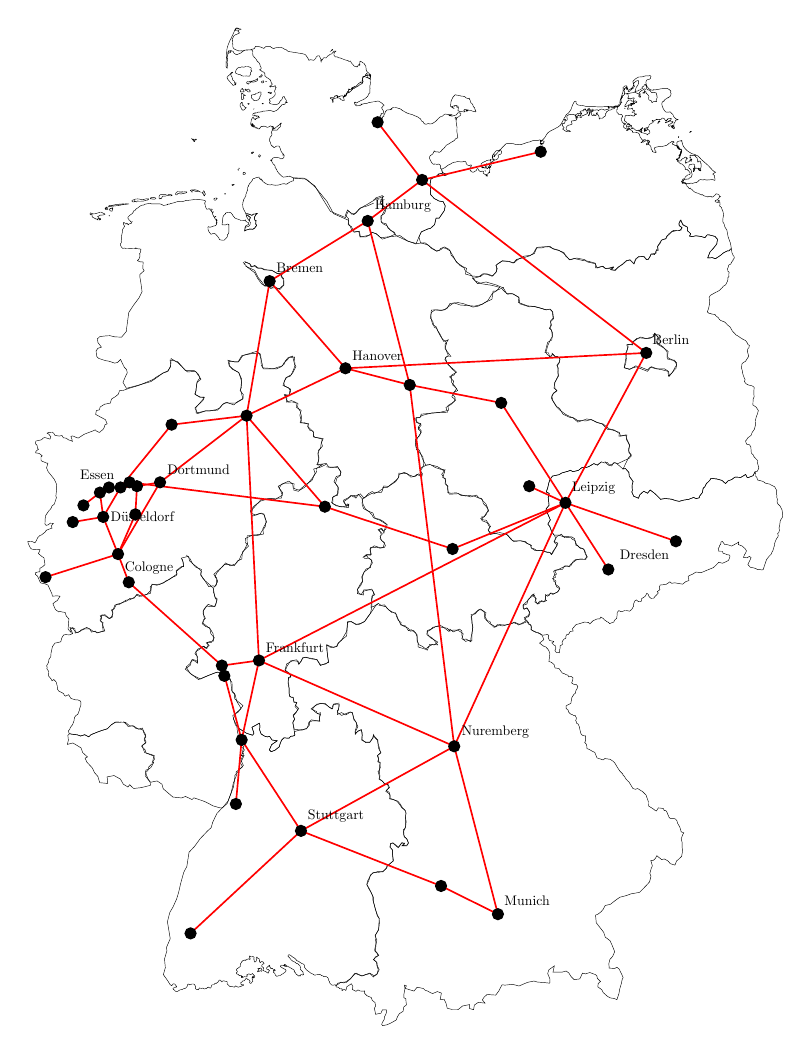
\begin{tikzpicture}

\definecolor{darkgray176}{RGB}{176,176,176}

\begin{axis}[
hide x axis,
hide y axis,
tick align=outside,
tick pos=left,
x grid style={darkgray176},
xmin=5.41798591613775, xmax=15.4935913085937,
xtick style={color=black},
y grid style={darkgray176},
ymin=46.8806100845338, ymax=55.4458555221558,
ytick style={color=black},
width=\linewidth,
height=1.28\linewidth
]
\addplot [line width=0.16pt, black]
table {%
8.70837306976324 47.7155570983886
8.71268272399902 47.7060623168946
8.71873188018799 47.6989135742188
8.71139812469477 47.6942787170411
8.69994831085216 47.6980361938477
8.69212532043457 47.6993370056152
8.68490028381348 47.6944847106934
8.67888832092291 47.6914443969727
8.66709423065197 47.6902580261231
8.66470623016357 47.6931343078614
8.66127586364757 47.6956634521484
8.66714191436779 47.6972236633302
8.67325878143305 47.6996383666992
8.67633533477795 47.705909729004
8.67048358917236 47.7113990783691
8.66622734069836 47.7148742675782
8.67177963256836 47.7169189453126
8.68023490905762 47.7178802490236
8.68641281127941 47.7136421203613
8.69133853912354 47.7165451049806
8.7006978988648 47.720142364502
8.70837306976324 47.7155570983886
};
\addplot [line width=0.16pt, black]
table {%
9.65046024322515 49.7763404846192
9.64671993255615 49.7352600097657
9.63594913482672 49.723991394043
9.63150024414062 49.6978416442872
9.68196868896479 49.7130584716797
9.734221458435 49.6947593688966
9.79042911529547 49.7175102233886
9.81357955932623 49.7102394104005
9.83292961120611 49.6546211242676
9.86216926574713 49.6362915039064
9.863450050354 49.6029090881348
9.84764003753668 49.5694007873536
9.84862041473389 49.5434799194336
9.88179874420172 49.5697097778321
9.92138957977306 49.5774688720703
9.93358993530279 49.5553703308107
9.9292192459107 49.5183410644531
9.92999839782721 49.4961585998536
9.98171043396007 49.4818916320802
10.0272397994996 49.4823112487794
10.0602989196777 49.5158119201661
10.0708284378052 49.5417518615723
10.0829687118531 49.5196914672852
10.1178789138795 49.4978485107423
10.1304388046265 49.4611091613771
10.1426296234131 49.4354286193848
10.1551504135133 49.3987312316896
10.1159391403199 49.3762817382813
10.1338491439819 49.3470115661622
10.1229391098022 49.3285102844239
10.1516275405884 49.3214416503906
10.1525583267212 49.2846908569336
10.1360483169556 49.2588005065918
10.1419305801392 49.2515106201172
10.1484308242798 49.2148399353028
10.1430997848511 49.1964187622071
10.1835393905641 49.1748085021974
10.2068395614625 49.1530303955078
10.2411603927612 49.1533889770509
10.2531890869142 49.1241607666016
10.2192888259888 49.0981292724609
10.2597303390504 49.0802116394044
10.2715091705323 49.0620002746582
10.271809577942 49.0436820983887
10.3179388046265 49.0331687927246
10.3584299087525 49.0189399719239
10.3934898376466 48.9899787902833
10.4167490005493 48.9682197570801
10.4391298294067 48.9606819152832
10.4558286666871 48.9457702636719
10.4669189453125 48.9272117614747
10.4555187225343 48.8977584838868
10.4665498733522 48.8644218444825
10.4607086181642 48.8238410949708
10.4493999481202 48.8091697692872
10.4437198638917 48.7981414794922
10.4323701858521 48.7760810852051
10.4378900527954 48.7575607299805
10.4490718841552 48.7426719665527
10.4770889282227 48.7239418029786
10.4938383102417 48.6941986083985
10.4712591171265 48.672248840332
10.4318799972534 48.6726303100586
10.4488496780395 48.6946296691895
10.4094686508179 48.6950187683105
10.3698692321777 48.6584815979004
10.3020696640015 48.6958007812501
10.2734708786012 48.6883697509767
10.2792100906373 48.6590385437012
10.301968574524 48.6369400024414
10.3018493652345 48.5963897705079
10.3073301315308 48.555690765381
10.2505998611451 48.5231018066407
10.2335996627809 48.5157890319825
10.2225599288942 48.4969596862794
10.1835803985596 48.4701118469238
10.1218395233155 48.4724998474122
10.0602903366089 48.4601097106934
10.0324802398682 48.4410095214843
9.99945068359381 48.3995895385743
9.98865890502935 48.3734092712402
10.011589050293 48.3403892517091
10.0457096099855 48.303810119629
10.0685291290284 48.2706718444825
10.0689191818237 48.2408599853516
10.0919904708862 48.1777496337892
10.1203107833863 48.1295204162598
10.1427507400513 48.1035804748536
10.1429491043091 48.0811614990234
10.1324081420899 48.0175285339355
10.0884895324708 47.9722709655763
10.110899925232 47.9388694763185
10.1001195907593 47.9014015197754
10.0948390960694 47.8639602661133
10.0949506759645 47.8452796936035
10.1060085296631 47.8416404724121
10.1281871795655 47.8156509399414
10.0951404571534 47.8078689575196
10.0731897354125 47.7852210998535
10.111780166626 47.7630691528321
10.1173086166382 47.7368392944336
10.1394691467285 47.7070999145508
10.1118392944337 47.6692314147949
10.0785303115844 47.6573905944824
10.0730514526367 47.6611213684083
10.0240898132324 47.6799316406251
9.97525978088385 47.6687393188477
9.92632865905762 47.6574096679688
9.84401988983154 47.6790313720703
9.81698989868164 47.6564903259277
9.78452968597423 47.6338920593263
9.74108982086193 47.6147994995117
9.70850086212164 47.6031799316406
9.67553997039806 47.6100387573242
9.64301013946533 47.5943489074708
9.61582946777344 47.5823020935059
9.60809707641602 47.5875549316407
9.59931564331055 47.5886344909669
9.59156322479254 47.5874824523926
9.58055114746094 47.5858955383301
9.56746578216564 47.5864715576173
9.55880260467541 47.5887489318848
9.55422782897955 47.591781616211
9.54609680175787 47.5974426269531
9.53862190246582 47.6039581298829
9.53589153289806 47.6126098632814
9.53309917449951 47.6181373596191
9.52856636047369 47.6193656921388
9.52529335021973 47.6254386901856
9.52381896972668 47.629135131836
9.52054023742676 47.6396560668946
9.51149272918713 47.6456222534181
9.50139141082775 47.6514587402344
9.48963165283209 47.6528053283691
9.48559665679932 47.6519966125489
9.4783754348756 47.6528930664062
9.47086143493658 47.651683807373
9.46423339843756 47.6545143127441
9.45750808715826 47.6581802368165
9.44812011718761 47.659523010254
9.43903255462652 47.6610946655273
9.42863941192627 47.6671295166016
9.42107486724848 47.6689834594727
9.4103507995606 47.6703491210938
9.39669227600092 47.6690368652344
9.39076995849609 47.6675834655762
9.3746967315675 47.6669807434082
9.36424160003662 47.6638488769532
9.35340976715088 47.664867401123
9.34339332580572 47.668212890625
9.33466625213634 47.6726226806641
9.32297325134272 47.6757583618165
9.31399726867681 47.6776199340821
9.30723381042486 47.6811218261718
9.29708385467535 47.6851539611817
9.29158020019531 47.689064025879
9.28154468536371 47.6937446594239
9.26723480224615 47.6994667053223
9.25749015808117 47.7048988342285
9.25014114379888 47.7104835510254
9.24290466308588 47.7170372009278
9.23632717132574 47.7226371765137
9.23141384124767 47.7293014526368
9.23014163970942 47.7369461059571
9.23065662384033 47.7432098388672
9.22443294525146 47.7482109069824
9.2136049270631 47.7519302368164
9.20805168151861 47.7532234191895
9.20123672485346 47.7544631958008
9.19145011901861 47.7590599060059
9.18303108215343 47.7624626159669
9.17338562011724 47.7661933898926
9.16315460205089 47.7707443237306
9.15264892578136 47.7739028930665
9.14535617828375 47.7753715515137
9.13589954376221 47.7795181274415
9.13059806823736 47.7854080200196
9.12322807312023 47.7908782958985
9.11534500122082 47.7942619323731
9.10388755798346 47.8007392883301
9.09918880462652 47.8025970458986
9.09108543395996 47.8041038513184
9.08247089385986 47.8089294433594
9.0749311447143 47.8122177124023
9.07011222839355 47.8168601989746
9.05317878723139 47.8216400146486
9.0467987060548 47.8235092163087
9.04012203216547 47.8222045898438
9.03320407867437 47.8167381286622
9.03183364868175 47.8129463195801
9.03997707366943 47.8063850402832
9.04921340942377 47.8014678955079
9.05444812774658 47.7963714599609
9.06152534484875 47.7916717529297
9.06891536712658 47.7852935791016
9.07866191864019 47.779483795166
9.08832454681402 47.7744712829591
9.09452724456787 47.7718505859376
9.1033754348756 47.7694129943848
9.11176872253429 47.7672576904297
9.12090778350841 47.7643127441406
9.12673091888422 47.7603073120117
9.13243103027355 47.7562713623046
9.13851070404064 47.7539863586426
9.15197944641108 47.7531929016113
9.15660190582281 47.7489128112794
9.1696834564209 47.7415885925294
9.17700290679932 47.7377548217775
9.17987060546881 47.7334213256836
9.18145370483398 47.7278709411622
9.18323516845703 47.723014831543
9.18505859375011 47.7189559936523
9.18371582031256 47.7103919982911
9.18822574615479 47.7066345214845
9.19218921661383 47.7022895812989
9.20068073272699 47.6975593566895
9.21247482299799 47.6903038024903
9.21541595458996 47.6844253540039
9.21637821197521 47.6759376525879
9.2215576171875 47.6689567565919
9.21742343902588 47.6667251586915
9.21097278594965 47.6650924682618
9.20100402832031 47.6685295104981
9.18757057189947 47.6692504882814
9.18506145477295 47.6643333435059
9.18147659301763 47.6574096679688
9.17087745666504 47.6605148315431
9.16667747497564 47.6618881225586
9.16502189636242 47.6571922302246
9.15844345092779 47.6579513549805
9.15294647216797 47.6605720520021
9.14853286743175 47.6659393310547
9.13695621490484 47.6681976318359
9.13035774230963 47.672836303711
9.12495899200434 47.6801300048829
9.11803817749035 47.6869888305665
9.11036586761475 47.688461303711
9.10772037506104 47.6919555664064
9.11163139343256 47.6946105957032
9.10950660705566 47.6994132995606
9.10383987426763 47.7048873901368
9.09731960296642 47.7083930969239
9.08959770202642 47.7112808227539
9.08130836486822 47.7134933471681
9.07031917572021 47.7178497314454
9.06135559082031 47.7216835021973
9.05045032501221 47.7261543273926
9.04244804382324 47.7277336120607
9.03370380401617 47.7314605712892
9.02359199523937 47.7336387634278
9.0131950378418 47.7391738891602
9.00182247161865 47.7456588745117
8.99239635467529 47.7479782104493
8.98550701141357 47.7454147338867
8.98817157745373 47.7411727905275
8.99635124206549 47.738452911377
9.0031938552857 47.7357177734375
9.01009559631348 47.731315612793
8.99729061126715 47.7321701049805
8.98511028289789 47.7368774414062
8.97660160064703 47.7398071289063
8.96861362457287 47.7408981323243
8.95772552490246 47.7418823242188
8.95046997070324 47.7406311035156
8.94417381286615 47.7381248474121
8.94136524200445 47.7318229675293
8.94789314270014 47.7273674011232
8.95422363281256 47.7254943847657
8.96321487426758 47.7214126586914
8.97292327880865 47.7169494628907
8.97875118255615 47.7149810791016
8.98491859436035 47.7132148742677
8.99152565002453 47.7115745544434
8.99672508239752 47.7102661132814
9.00337696075445 47.7057037353517
9.00872898101807 47.7000312805176
9.00550270080566 47.6943664550782
8.99800872802729 47.6882476806641
8.99105644226086 47.6840248107911
8.98582363128662 47.6820831298828
8.9809455871582 47.6804008483888
8.9737167358399 47.6746253967286
8.96322441101086 47.6727447509766
8.95596313476568 47.6699180603028
8.94959831237799 47.6669654846191
8.94071388244635 47.661678314209
8.92500972747808 47.6613731384278
8.91370391845697 47.6579627990723
8.90520191192638 47.6567687988281
8.89183425903332 47.6552238464357
8.87854003906256 47.6658515930176
8.87299537658691 47.6762657165527
8.86657619476318 47.6817436218263
8.860016822815 47.6839294433595
8.8548383712768 47.6879997253419
8.85904026031494 47.6944732666015
8.85572910308832 47.6989555358886
8.85916233062738 47.7020797729493
8.86531639099127 47.7003784179689
8.86726093292248 47.6974258422852
8.87013912200939 47.6968231201172
8.87787246704107 47.6989212036133
8.87658691406256 47.7021064758301
8.87370681762707 47.7049293518066
8.87209320068371 47.7085342407228
8.8550767898559 47.7081947326661
8.84860324859625 47.7121810913087
8.84465408325201 47.7162895202638
8.83664035797131 47.7179412841796
8.82831192016613 47.7151031494141
8.82244777679455 47.7168884277344
8.82460021972668 47.7212753295899
8.82076835632319 47.7217826843262
8.81555271148682 47.7270812988282
8.80809402465832 47.7294616699219
8.81241321563721 47.7334556579591
8.81119728088379 47.7357864379883
8.80929374694836 47.740249633789
8.80632114410412 47.7417984008789
8.79995632171642 47.7387847900391
8.79578304290783 47.7325515747071
8.78918266296392 47.7320938110352
8.78331184387207 47.7271347045898
8.77269458770752 47.7218818664551
8.77110385894775 47.7186965942382
8.77216911315918 47.7119445800782
8.78043079376226 47.7097396850585
8.79748630523687 47.7072372436525
8.79992485046398 47.7030181884767
8.80505752563488 47.7002639770508
8.80853271484381 47.6978797912598
8.80264472961431 47.69637298584
8.79735946655279 47.6904220581056
8.79629611968994 47.6814765930176
8.79178714752209 47.6793975830079
8.78179740905773 47.6826667785645
8.77375507354742 47.6864814758301
8.76686096191406 47.6908988952638
8.75304985046381 47.6949806213379
8.73966598510742 47.6966819763184
8.72960376739502 47.7051963806153
8.73334026336664 47.7132644653321
8.73743343353266 47.7203712463379
8.73475837707525 47.7235221862794
8.72563266754162 47.7267379760742
8.71699523925793 47.7299385070801
8.7134313583374 47.7350196838379
8.71482753753668 47.7417640686036
8.71932792663574 47.7455215454102
8.72465801239019 47.7497825622559
8.73334789276123 47.7511138916017
8.74229717254633 47.7527999877931
8.74053764343267 47.7580528259278
8.73138332366943 47.7633056640626
8.72906875610357 47.7671165466309
8.71936130523676 47.7701454162598
8.71004867553722 47.7696342468262
8.70104694366461 47.7657661437988
8.69786643981939 47.7621459960939
8.69301700592052 47.7624855041504
8.68807888031006 47.7706794738769
8.68549633026123 47.7755165100098
8.68839740753174 47.7802963256837
8.68372154235846 47.7855491638183
8.68181514739996 47.7921981811523
8.67188072204596 47.793399810791
8.66308689117426 47.7966003417969
8.66181182861334 47.8009719848633
8.65870666503906 47.8051910400391
8.65114688873291 47.8051300048828
8.64780712127691 47.7999229431152
8.64606094360352 47.7959175109863
8.64925193786632 47.7908935546876
8.64937305450445 47.7808074951172
8.64617824554449 47.7741088867188
8.64328956603998 47.771224975586
8.64021873474127 47.7699737548829
8.63050937652588 47.7657737731934
8.62617301940929 47.7697601318361
8.62173557281494 47.7739295959473
8.62348842620855 47.7819099426271
8.62011241912847 47.7851753234863
8.61669158935558 47.7901153564454
8.61961269378662 47.7944793701172
8.62158775329601 47.8017196655273
8.61474895477295 47.8076362609864
8.60294437408453 47.8091011047364
8.59474372863775 47.8063049316406
8.59028244018566 47.8076667785646
8.58341407775879 47.8077354431152
8.57697010040278 47.8070449829102
8.57386779785156 47.8120498657227
8.5686759948731 47.8143997192384
8.56313991546631 47.8113059997558
8.56232833862305 47.7999725341797
8.56805992126465 47.7970008850097
8.57480812072748 47.7928314208985
8.57164669036877 47.7875518798828
8.56379985809326 47.7875175476074
8.55491924285894 47.7910957336426
8.5483484268189 47.7901306152344
8.53843688964849 47.7880249023438
8.52550315856928 47.7843322753906
8.52108097076422 47.778305053711
8.51064491271978 47.7829437255861
8.50574398040771 47.7810249328613
8.49781322479248 47.7789306640626
8.49124526977545 47.7793998718263
8.48542690277111 47.778175354004
8.47800254821772 47.7733230590821
8.47058391571051 47.7679901123047
8.46823215484619 47.7631912231445
8.46524238586431 47.759693145752
8.45897006988537 47.757610321045
8.45654582977306 47.7513618469239
8.45364570617687 47.7474555969238
8.45261192321789 47.7400283813478
8.45591640472406 47.7332649230958
8.44421100616466 47.727840423584
8.44092559814453 47.7240943908693
8.43522071838379 47.723545074463
8.42614078521734 47.718246459961
8.41727733612055 47.7165603637696
8.4077291488648 47.7081985473634
8.40561485290533 47.7034225463868
8.41038513183594 47.7012672424316
8.41483974456793 47.6950988769531
8.41806221008301 47.690773010254
8.41506671905518 47.6867370605469
8.40631771087641 47.6838836669922
8.40472316741949 47.6787452697753
8.41301155090343 47.6720390319825
8.42396926879894 47.6713371276855
8.43025398254395 47.6682739257813
8.43540000915533 47.6643829345703
8.44223690032959 47.6607704162599
8.45190620422369 47.6595458984376
8.46172237396246 47.6596946716309
8.46718406677246 47.6611022949218
8.4658727645874 47.6533050537109
8.46818065643322 47.6453437805177
8.47563457489025 47.6434135437013
8.47862529754644 47.6453018188477
8.47322654724132 47.6467018127441
8.47423934936529 47.6486663818361
8.47744941711431 47.6503562927246
8.47510719299316 47.6544380187989
8.48215579986572 47.6535263061523
8.48421001434338 47.6495628356933
8.48891162872314 47.6482238769532
8.49495410919184 47.6478042602539
8.49670696258551 47.6515541076661
8.50172328948975 47.6520919799806
8.52180194854748 47.6509819030762
8.53375244140619 47.651035308838
8.53589725494385 47.6544456481934
8.5318603515625 47.6618843078614
8.5327262878418 47.6667861938478
8.53828525543219 47.663917541504
8.54125499725336 47.6647453308106
8.54394912719721 47.6703720092774
8.56136226654064 47.674674987793
8.57065582275396 47.6691246032715
8.57901000976562 47.6675910949708
8.58792495727545 47.6708793640138
8.59741973876964 47.6745796203613
8.60257434844971 47.6769714355469
8.61126804351807 47.6683006286621
8.61979579925537 47.6639213562012
8.62553977966314 47.6598205566406
8.6293888092041 47.6535186767578
8.6250953674317 47.6458625793458
8.61572360992437 47.6416931152344
8.60432529449474 47.64315032959
8.60906410217291 47.6462898254396
8.61533355712902 47.6501846313478
8.61017990112305 47.6560173034669
8.60499000549316 47.6551628112794
8.59684658050548 47.6471939086914
8.59804725646984 47.6345481872559
8.60279464721685 47.6254615783692
8.60586929321295 47.6168937683107
8.59806728363037 47.6113128662109
8.59033775329601 47.6057624816895
8.58634185791027 47.6028289794922
8.58178424835205 47.5997772216797
8.57199287414551 47.6011924743653
8.56536293029791 47.609031677246
8.5719194412232 47.6148300170899
8.57200813293457 47.6178207397461
8.56497573852539 47.6212997436523
8.55906963348389 47.6276054382325
8.54800891876221 47.6295013427734
8.54068088531494 47.631519317627
8.53899097442638 47.6347961425781
8.53183078765881 47.636344909668
8.52302646636969 47.6379623413087
8.51887035369879 47.6365852355956
8.51397514343267 47.6293640136719
8.50899219512945 47.6270828247071
8.50658226013195 47.6221199035645
8.49603366851807 47.6191177368165
8.48259353637695 47.618637084961
8.47723865509033 47.6142082214356
8.47123908996576 47.6092948913575
8.46470355987549 47.6075019836426
8.45824337005615 47.6053199768066
8.45950031280518 47.6011848449708
8.46142673492437 47.5941162109376
8.46748924255382 47.5896759033204
8.47150897979731 47.5885543823243
8.48195743560791 47.5894660949708
8.49204444885254 47.5909423828125
8.48968315124512 47.582763671875
8.47814178466803 47.581356048584
8.47262668609625 47.5788688659669
8.45789909362799 47.5765266418457
8.44715595245361 47.5738372802735
8.43453121185314 47.5713272094727
8.42343139648443 47.5707511901857
8.41617393493664 47.5744094848633
8.40685558319092 47.577709197998
8.39744186401379 47.580150604248
8.38742160797125 47.5745353698731
8.38315677642822 47.5703124999999
8.37329864501964 47.5716209411622
8.35743618011486 47.5742416381837
8.33047389984131 47.5747642517091
8.32132053375244 47.5784606933595
8.31454944610596 47.5834808349609
8.29977798461925 47.5913276672364
8.29470157623297 47.5965003967286
8.29558563232422 47.6082000732422
8.29330921173107 47.6126823425294
8.28142738342297 47.6163368225099
8.27288818359375 47.6161689758302
8.26095867156988 47.6178894042969
8.25420379638672 47.620059967041
8.24035167694092 47.6181640625001
8.23482704162603 47.6162605285645
8.22952365875256 47.6115531921388
8.22291278839117 47.6130638122559
8.21815490722656 47.622573852539
8.2067956924439 47.6262550354005
8.19632816314709 47.6241264343262
8.18986892700201 47.6179962158203
8.18776798248302 47.6148719787598
8.18297386169434 47.6098442077638
8.1759462356568 47.6084938049318
8.17027664184582 47.6041145324708
8.16212463378912 47.5996131896973
8.15146446228022 47.6012763977052
8.14140129089355 47.5982208251953
8.13720417022705 47.5918617248536
8.13370609283453 47.5890541076661
8.11497402191168 47.5892066955567
8.10432720184326 47.5844078063965
8.10028171539307 47.5709686279297
8.09580707550049 47.5655212402345
8.08651161193859 47.5628051757813
8.07672309875494 47.5660247802735
8.0710134506225 47.5700035095216
8.06526947021496 47.569881439209
8.05796813964849 47.5688858032227
8.04987525939953 47.5635643005371
8.03913402557379 47.5593109130859
8.01532363891607 47.5568771362305
8.00687599182135 47.5593643188477
7.9995379447937 47.5624160766602
7.98657608032238 47.5614891052246
7.97047805786133 47.5616455078126
7.9571299552918 47.56400680542
7.95049285888666 47.5555419921876
7.94698715209961 47.5500297546387
7.93535804748541 47.5523071289063
7.91738605499279 47.5539131164551
7.90874481201172 47.5603256225587
7.90722417831415 47.5685386657715
7.91026782989508 47.5759582519532
7.90484380722052 47.5839538574219
7.89448404312134 47.5920257568361
7.88652515411371 47.5948944091798
7.86763381958008 47.5952033996581
7.85302877426147 47.5913429260255
7.84006214141851 47.5888862609864
7.83285522460938 47.5925521850587
7.82077217102056 47.5946998596192
7.81562089920044 47.5909194946289
7.8118138313294 47.5827026367187
7.80856800079346 47.5754699707031
7.80025911331177 47.5706901550294
7.79436206817638 47.5646133422852
7.78735065460205 47.5618591308595
7.77046012878424 47.5591278076172
7.75716018676769 47.5557289123535
7.75042819976801 47.5516777038575
7.72458600997925 47.5497512817383
7.70842981338501 47.5442657470704
7.69653606414795 47.5389595031738
7.68693876266479 47.5361022949219
7.66517782211309 47.538833618164
7.6569390296936 47.5460662841798
7.65017890930176 47.5495491027833
7.64268398284912 47.5519828796387
7.63682699203503 47.5587043762208
7.63945198059076 47.5631065368653
7.64800930023193 47.56498336792
7.66280603408825 47.5679054260255
7.6720399856568 47.5717277526857
7.67832088470459 47.5705413818359
7.68170309066772 47.5735359191895
7.67740488052362 47.5763473510743
7.67208814620966 47.5850105285645
7.66676616668701 47.5863838195802
7.6645069122315 47.5893058776855
7.65889120101934 47.5940628051758
7.64944601058954 47.5961647033691
7.63876819610596 47.5969467163087
7.63531112670898 47.5926742553711
7.62842178344721 47.5879516601563
7.62015104293823 47.5820465087891
7.60277509689337 47.5896835327149
7.57183313369745 47.6214981079102
7.52001142501837 47.6680755615235
7.5438866615296 47.7225837707521
7.53389596939093 47.7902183532715
7.56260490417486 47.853084564209
7.55832004547131 47.8812789916993
7.60334253311157 47.9485626220703
7.56931543350231 48.0806770324707
7.58777141571039 48.1280059814454
7.59949970245361 48.1556320190431
7.63713073730469 48.195873260498
7.68145990371715 48.2596397399903
7.70507860183727 48.3096351623536
7.73096609115606 48.3822059631348
7.76616191864014 48.4639739990235
7.80516195297247 48.5135002136231
7.83175373077404 48.6232795715332
7.8962516784668 48.6672096252442
7.96770238876343 48.7297859191895
8.01622200012213 48.7623977661132
8.05623722076416 48.7896461486816
8.10069656372065 48.8154487609864
8.11810111999506 48.8563079833984
8.16850566864019 48.9245033264161
8.23029518127453 48.9672966003419
8.2952995300293 49.0041503906251
8.3408002853393 49.0840110778809
8.36952018737793 49.1632385253907
8.40528869628912 49.2203521728515
8.40367889404291 49.2499122619629
8.48058891296392 49.289821624756
8.45673084259039 49.3183708190919
8.49954032897961 49.3787803649902
8.46553993225098 49.3775291442872
8.50355815887451 49.4229621887208
8.44516944885254 49.4612503051757
8.44361877441412 49.501579284668
8.44622039794922 49.5861892700195
8.5276603698731 49.5521697998047
8.60262966156006 49.5363311767579
8.61937904357916 49.5515289306641
8.59504890441895 49.5983886718749
8.68616867065435 49.6305313110352
8.69249820709229 49.6087417602539
8.68750858306879 49.5793113708497
8.70555973052984 49.5469322204591
8.74616146087658 49.529811859131
8.78079032897955 49.5234107971192
8.80945873260498 49.527759552002
8.83880996704113 49.4992408752442
8.90242958068853 49.4930992126465
8.86804866790783 49.4779396057128
8.83375930786138 49.4626922607422
8.80581855773926 49.4220085144044
8.82904815673828 49.4079818725587
8.87488937377924 49.4197616577149
8.92646980285656 49.4459686279298
8.93756866455078 49.4716491699219
8.95446014404308 49.4974212646485
8.9830493927002 49.5160217285156
9.04674911499023 49.5128517150878
9.06380844116217 49.527629852295
9.1041898727417 49.5314521789551
9.11559867858898 49.5388298034668
9.10931968688976 49.5645904541017
9.18978977203375 49.5793418884278
9.25874996185303 49.5864486694337
9.27552032470697 49.6085815429688
9.28634071350103 49.6381416320802
9.31462955474865 49.6565589904786
9.41805934906012 49.6452293395996
9.41161823272716 49.6711921691895
9.4280300140382 49.6971321105957
9.39357852935802 49.7045593261719
9.35892868042004 49.7193984985352
9.34142971038824 49.7342185974122
9.31266880035406 49.7416610717773
9.36345958709722 49.767520904541
9.43115901947021 49.7861289978028
9.48233985900879 49.77885055542
9.51671981811523 49.7641105651855
9.56256961822521 49.7420196533203
9.58343982696545 49.7794418334961
9.65565872192388 49.7875595092775
};
\addplot [line width=0.16pt, black]
table {%
10.1338596343995 50.5499992370606
10.175030708313 50.5463218688965
10.2220582962036 50.5388488769532
10.25749874115 50.5127105712891
10.3105001449586 50.4940490722657
10.3458290100097 50.4828720092773
10.3696393966674 50.4418487548828
10.3815002441407 50.4269409179687
10.3933992385864 50.4082794189453
10.4287796020508 50.3896713256837
10.4935398101807 50.3711090087891
10.5171899795533 50.3487510681153
10.5583114624024 50.3525505065919
10.5996913909913 50.3190307617188
10.5999088287354 50.2853622436525
10.605890274048 50.2666816711426
10.6177797317505 50.2442588806153
10.6647691726684 50.2294197082521
10.7230186462403 50.1997985839844
10.7518301010132 50.2447204589844
10.8093795776368 50.241310119629
10.8495798110962 50.2638320922853
10.8035392761232 50.2822418212891
10.7690296173095 50.2932815551758
10.7172508239746 50.322940826416
10.7224493026733 50.3526611328126
10.7798700332641 50.3675994873048
10.8199300765991 50.3825187683106
10.8772802352905 50.3937797546387
10.9118385314942 50.3827590942383
10.9868106842042 50.3459205627443
10.9981107711791 50.3644790649415
11.0385084152223 50.3423614501954
11.1132392883301 50.3648986816407
11.1421594619752 50.3501586914063
11.1421003341676 50.3167495727539
11.1596403121949 50.2834587097168
11.1940393447877 50.2872505187988
11.2516689300537 50.2651901245118
11.2518787384034 50.2911415100098
11.2640590667726 50.3320198059083
11.2763004302979 50.3803787231446
11.2649793624878 50.4100494384766
11.2652893066406 50.4397888183594
11.2540006637574 50.4806289672852
11.3007707595826 50.480812072754
11.347978591919 50.5144386291504
11.3831501007081 50.514560699463
11.4180603027344 50.492359161377
11.4175081253052 50.4514503479003
11.4523401260377 50.4254989624024
11.4814081192017 50.4069709777833
11.5165004730225 50.395881652832
11.5514888763429 50.3810615539552
11.5987586975097 50.3997993469238
11.6690998077392 50.3962516784669
11.7279195785524 50.4038391113282
11.763279914856 50.4113807678224
11.781060218811 50.4188995361329
11.8332996368409 50.4041213989258
11.8683385848998 50.4042091369629
11.9332876205445 50.4230957031251
11.9508810043336 50.4051361083985
11.9728994369507 50.40087890625
11.988410949707 50.3786888122559
11.980833053589 50.3621330261232
11.9984741210938 50.3524780273438
12.042724609375 50.337890625
12.0652704238892 50.3379096984864
12.0980758666992 50.3269500732423
12.1192445755005 50.3130340576173
12.1273336410524 50.2997283935546
12.1371698379517 50.2821121215821
12.0858602523804 50.2553520202638
12.1089019775391 50.2439460754395
12.1319217681885 50.2320747375489
12.161280632019 50.2252082824708
12.1852025985718 50.2088623046876
12.1989192962646 50.1956214904786
12.2102556228639 50.171459197998
12.1990604400635 50.1118202209473
12.2236337661744 50.1068382263184
12.2387990951538 50.1005210876465
12.2619924545289 50.087646484375
12.2671489715576 50.074031829834
12.2734403610229 50.0612945556642
12.3019199371339 50.058864593506
12.3234615325928 50.0559158325196
12.3403053283693 50.0390205383301
12.3644390106201 50.0203819274903
12.3873596191406 50.0163803100587
12.4103908538818 50.0084609985353
12.4300937652589 50.0047760009766
12.4392223358154 49.9918441772462
12.4683113098146 49.9958801269531
12.4915103912355 49.9839515686036
12.4858713150024 49.9634895324708
12.474949836731 49.9445724487304
12.4975881576538 49.9344406127931
12.5331840515136 49.930633544922
12.5491809844971 49.9181823730469
12.5444335937501 49.9042472839355
12.526593208313 49.8848419189454
12.5192785263063 49.8639907836915
12.5033111572267 49.8559761047363
12.4783086776733 49.8320312500001
12.4698915481567 49.8037109375001
12.4658308029174 49.7857551574708
12.4473314285279 49.779411315918
12.4087495803834 49.7661895751954
12.4084739685059 49.7448501586915
12.4312286376953 49.7328186035157
12.4406900405884 49.7154693603517
12.4583139419557 49.7031402587891
12.4862108230591 49.6961135864258
12.4951152801514 49.6907997131347
12.516598701477 49.6916007995605
12.5329446792603 49.6718978881837
12.5283613204957 49.6570854187012
12.5227203369141 49.6488914489746
12.5303115844727 49.6449050903321
12.536660194397 49.6285514831544
12.5528450012207 49.6246528625488
12.55885887146 49.6174087524415
12.5703268051148 49.5979232788087
12.5753774642945 49.5801544189454
12.5844507217407 49.5536079406739
12.5942611694337 49.5408020019531
12.6154766082764 49.5331649780273
12.6458301544191 49.5310592651367
12.6443939208985 49.4944534301758
12.6328067779542 49.4800148010255
12.6467456817628 49.471939086914
12.6570024490356 49.4582099914551
12.6610746383668 49.4321670532227
12.6898450851441 49.4251441955566
12.7193031311036 49.4136276245117
12.7555837631226 49.4025840759278
12.7829885482788 49.3591842651368
12.8576192855836 49.3436088562013
12.8767499923707 49.3545112609864
12.9411487579346 49.3486595153809
12.9804162979126 49.3320274353027
13.0011110305786 49.3171577453613
13.0326108932496 49.282730102539
13.0609884262086 49.2558517456055
13.0954179763795 49.2338256835938
13.0999822616577 49.2223091125489
13.1145906448364 49.2165374755859
13.1311626434327 49.1972122192383
13.1542034149171 49.1806259155275
13.1691198349 49.1725578308107
13.1861791610718 49.1554489135743
13.2177381515503 49.1211318969728
13.2482128143311 49.1143608093263
13.2749977111816 49.1206436157227
13.3338308334351 49.0973205566407
13.3769292831421 49.0707321166993
13.4074516296388 49.0151824951172
13.4071636199951 48.9933280944824
13.4084062576295 48.9843482971191
13.4374084472656 48.9726219177247
13.4663915634155 48.9608879089355
13.4885816574097 48.9487113952637
13.5033550262451 48.9451217651367
13.5268354415895 48.9692535400391
13.5613679885865 48.9668998718262
13.5891103744508 48.9641113281251
13.5981464385987 48.9477691650392
13.6144990921021 48.9491691589357
13.6252593994141 48.9433708190918
13.634614944458 48.9307212829589
13.6433172225952 48.9167137145997
13.6576251983643 48.8959197998046
13.6675214767456 48.8887939453126
13.697340965271 48.8847885131837
13.72260761261 48.8853912353517
13.736798286438 48.8813133239747
13.7519311904907 48.8700218200685
13.7616329193116 48.847972869873
13.7695722579957 48.8394012451173
13.7775077819825 48.8308258056642
13.7888803482057 48.8169898986818
13.804204940796 48.7826385498047
13.8359575271606 48.7750511169435
13.8235597610474 48.7606811523437
13.8042993545533 48.7282905578614
13.8144683837891 48.7027778625489
13.8162641525269 48.660327911377
13.8200798034668 48.6297721862793
13.8099441528321 48.59090423584
13.7608966827392 48.5613784790039
13.7489957809449 48.5570755004883
13.7286520004272 48.522789001465
13.6723461151123 48.5339279174805
13.6453313827515 48.5543746948242
13.6019525527955 48.5706596374512
13.5657234191895 48.5662689208986
13.5085992813111 48.5963897705079
13.4908790588379 48.5746192932128
13.466835975647 48.5603561401368
13.435447692871 48.5598144531251
13.4545402526856 48.516300201416
13.4411983489991 48.4977531433105
13.4236793518068 48.4577789306642
13.437659263611 48.4363365173339
13.4201545715332 48.3915367126465
13.3686418533325 48.3558235168458
13.297986984253 48.3099098205566
13.1977338790894 48.2989654541016
13.1412687301636 48.2855300903321
13.058403968811 48.2717361450196
13.0034379959107 48.2465362548829
12.9463319778442 48.21732711792
12.8824644088746 48.2075424194337
12.8559894561769 48.1768112182618
12.8324937820435 48.1590919494629
12.7974910736085 48.1415252685548
12.7647256851196 48.1320304870606
12.7737283706666 48.0727195739747
12.8640136718749 47.9982185363769
12.8832569122315 47.960521697998
12.91832447052 47.9440841674805
12.942084312439 47.9312858581543
12.9666528701782 47.8963623046876
12.9973659515381 47.8474273681642
12.971534729004 47.809497833252
12.9376850128173 47.7854537963867
12.9261684417725 47.7532806396484
12.9307203292847 47.7189598083497
12.9976987838746 47.7162590026857
13.023491859436 47.7256660461425
13.05153465271 47.7115440368652
13.0790977478027 47.6757202148438
13.0995168685914 47.6454505920411
13.0879936218263 47.6294746398927
13.076530456543 47.5950012207032
13.0589895248414 47.5579109191895
13.048776626587 47.5206642150879
13.0242395401 47.4727592468262
12.9931430816652 47.4817504882814
12.9473209381104 47.4861221313477
12.9130592346192 47.4967422485352
12.857219696045 47.5283584594727
12.8396644592286 47.5513954162598
12.7920913696288 47.572364807129
12.7970190048219 47.5989112854004
12.8250036239625 47.6143913269044
12.7875633239747 47.6385955810546
12.7791461944581 47.6621894836426
12.756314277649 47.670021057129
12.6943368911743 47.6846656799316
12.6443052291871 47.6741828918457
12.6053342819214 47.6792488098145
12.5741014480591 47.6348838806152
12.5056247711183 47.6290473937989
12.4667396545411 47.6541442871094
12.4402570724487 47.6813812255859
12.4086751937867 47.6962356567383
12.3621530532838 47.6880836486816
12.2970485687257 47.6876602172852
12.2479887008668 47.6875000000001
12.2648983001709 47.7364311218262
12.1988801956177 47.7064285278321
12.1838417053223 47.6771430969239
12.2121057510375 47.6326789855958
12.2092800140381 47.6012001037598
12.1544904708863 47.6053619384767
12.0608491897584 47.6101417541504
12.0168094635009 47.618049621582
11.9396581649781 47.6077308654786
11.8348293304444 47.5792884826661
11.7907781600952 47.5871620178224
11.7553968429565 47.5922279357911
11.6676912307739 47.5862731933595
11.6300992965699 47.5884780883789
11.608759880066 47.5632514953614
11.5926008224488 47.5417556762695
11.5534496307373 47.5084190368652
11.4484786987305 47.5131607055665
11.4125556945802 47.4922332763672
11.3905820846558 47.4707946777344
11.4240808486939 47.4456214904786
11.3416061401367 47.4518241882324
11.2938966751099 47.4301986694337
11.2849788665772 47.3948822021484
11.2355899810791 47.4031791687012
11.2359476089478 47.434196472168
11.1511888504028 47.4235649108887
11.0972509384155 47.3957214355469
11.0232343673707 47.3962020874023
10.9648666381835 47.4060363769532
10.9496288299561 47.4460220336915
10.9265918731689 47.4762153625488
10.8790102005005 47.4740905761719
10.8887186050416 47.5056991577148
10.8941373825074 47.5243263244629
10.845311164856 47.5358276367188
10.7874727249146 47.5203704833984
10.7612400054932 47.5273323059082
10.7269411087036 47.5400238037109
10.6975908279419 47.5456695556642
10.6754474639893 47.5601463317871
10.599970817566 47.5698318481446
10.5791826248169 47.5540237426758
10.5614671707154 47.5397911071778
10.453429222107 47.5610198974609
10.4698295593262 47.5809860229492
10.4459648132324 47.5856666564941
10.4517965316772 47.5575599670411
10.4396677017212 47.5170974731445
10.4384460449219 47.4881553649903
10.4626731872559 47.4797286987305
10.4648036956788 47.4579162597657
10.4700441360474 47.43265914917
10.4349317550659 47.4137001037598
10.4302892684937 47.3823738098145
10.3843297958375 47.3636360168458
10.3621091842652 47.3408699035645
10.3452501296998 47.3139190673829
10.2851896286011 47.2917213439943
10.2363986968995 47.2772216796876
10.1813392639161 47.2699394226075
10.1692867279053 47.2791099548341
10.1761407852174 47.2925491333009
10.2038888931274 47.3231086730958
10.2019653320312 47.3358116149902
10.2262201309204 47.3686408996582
10.2268695831299 47.3929176330567
10.178505897522 47.3934936523437
10.1606607437134 47.3672485351563
10.0961999893189 47.3585090637207
10.0808954238892 47.4045257568361
10.0949831008912 47.4233703613282
10.0886058807373 47.4506454467774
10.0553798675537 47.466869354248
10.0433826446534 47.4893760681152
9.99119472503662 47.5032081604005
9.96118831634516 47.5230407714844
9.96367740631115 47.5411643981935
9.94481468200684 47.5389022827148
9.90803241729742 47.54056930542
9.88100242614757 47.5485458374025
9.85710906982422 47.5382194519043
9.81310176849371 47.5524559020997
9.82004165649414 47.5752944946289
9.8015394210816 47.5971603393556
9.74723911285395 47.5741691589357
9.73667144775402 47.5472412109375
9.73229598999023 47.5453567504883
9.72355270385748 47.5503120422364
9.70933628082275 47.5516967773438
9.70098495483398 47.5486297607422
9.6951141357423 47.5439605712892
9.68802356719971 47.5443000793457
9.68502902984631 47.547721862793
9.68946456909191 47.5498428344728
9.69080257415777 47.5552864074708
9.68641662597656 47.5583343505859
9.67394638061529 47.5574188232422
9.66531181335461 47.5581893920899
9.65615940094 47.5600166320801
9.65301132202154 47.5647773742676
9.64020729064953 47.5679283142089
9.6367712020874 47.5708465576173
9.63286781311035 47.5715637207032
9.62277412414551 47.570915222168
9.61513328552257 47.5761795043946
9.61192798614502 47.5812339782716
9.62124824523926 47.5862388610839
9.63741016387951 47.6017799377442
9.67562007904064 47.6063308715821
9.71927928924561 47.6107521057129
9.74122905731201 47.6073989868165
9.7954092025758 47.637722015381
9.82240962982183 47.660270690918
9.86045074462902 47.6791992187501
9.93178081512451 47.657440185547
9.98069953918468 47.6687507629395
10.0295095443726 47.6761589050294
10.0674896240234 47.6497421264649
10.0895986557007 47.6650619506837
10.1118097305298 47.6729621887208
10.1283702850342 47.7069396972656
10.1117887496948 47.7367897033691
10.1062688827515 47.7667694091796
10.0676794052124 47.7851715087891
10.1006603240967 47.8041801452637
10.1336984634399 47.8194389343262
10.1059894561769 47.8453788757325
10.089409828186 47.8489799499512
10.083830833435 47.8601303100587
10.1000576019287 47.9088706970215
10.0942192077638 47.9499092102052
10.093999862671 47.9760589599609
10.132378578186 48.0212707519531
10.137399673462 48.0811004638671
10.1371698379517 48.1072616577148
10.1147499084473 48.1294593811035
10.0919103622437 48.1852188110353
10.0632390975952 48.2482414245607
10.0628490447998 48.2780303955079
10.0400190353395 48.311149597168
10.011480331421 48.3478202819825
9.98871994018566 48.3697013854981
10.0161504745483 48.4073295593263
10.0324296951295 48.4447288513183
10.0658416748047 48.4639205932617
10.1275291442872 48.4652099609376
10.1835393905641 48.4738197326661
10.2281589508057 48.4970588684082
10.2392406463624 48.5158500671388
10.2562789916992 48.5267295837403
10.3129796981812 48.5556297302247
10.3018903732301 48.6074600219727
10.3019781112672 48.6406211853027
10.2677593231202 48.6626586914062
10.2791976928711 48.6920700073242
10.3077697753906 48.6958007812501
10.3755283355712 48.662109375
10.4151096343995 48.6986618041993
10.4432096481324 48.690990447998
10.4149894714356 48.6728019714357
10.4825496673585 48.6795310974121
10.4938497543336 48.6978912353517
10.4715013504029 48.7313690185547
10.443440437317 48.7427101135254
10.4379081726075 48.7612495422364
10.4379787445069 48.7760314941407
10.4324893951417 48.7982521057129
10.4550285339356 48.8091201782228
10.4607696533203 48.8349189758302
10.4609394073487 48.8644714355469
10.4555492401122 48.9014587402344
10.4557399749755 48.9309997558595
10.4558382034302 48.9494590759277
10.4335298538209 48.9607200622559
10.4167718887329 48.975570678711
10.3932991027833 49.0009803771973
10.3641099929811 49.0226593017579
10.312189102173 49.0331115722656
10.2661209106446 49.0399513244629
10.2713899612427 49.0693397521974
10.2595386505128 49.0912094116212
10.2249002456665 49.1055221557618
10.2645597457885 49.1279411315917
10.241008758545 49.1607208251953
10.2067699432374 49.1567001342773
10.1777496337891 49.1784210205078
10.1374588012695 49.1926918029786
10.1427192687988 49.214771270752
10.1247301101685 49.2550086975098
10.1417598724366 49.2588500976564
10.1409692764282 49.2919197082521
10.1515302658082 49.3251190185547
10.1228504180908 49.3321914672852
10.1336507797241 49.3543701171876
10.1215295791627 49.3800086975098
10.1608381271362 49.398780822754
10.1312484741212 49.4353294372559
10.1246318817138 49.4647407531739
10.1235790252686 49.4979019165039
10.0885486602783 49.5234298706054
10.0710792541504 49.5343589782716
10.0660009384156 49.5158615112305
10.0216703414918 49.4785690307618
9.97614860534674 49.478141784668
9.92974090576166 49.5035514831543
9.93437862396246 49.5331802368164
9.92776012420654 49.5590209960938
9.92124938964849 49.5811805725098
9.87067890167248 49.5621910095216
9.84847831726074 49.5471801757813
9.85333061218267 49.569450378418
9.88053894042963 49.6030616760253
9.85631942749029 49.6399612426759
9.83248996734613 49.6657600402833
9.8134298324585 49.7139587402345
9.7847194671632 49.7174720764161
9.72245979309076 49.7021217346191
9.68297863006603 49.6907005310059
9.63645935058594 49.7127990722657
9.63018035888678 49.7276687622071
9.64653968811029 49.7389907836914
9.65614891052257 49.7763710021973
9.58359909057629 49.775718688965
9.57377910614014 49.742099761963
9.52826023101801 49.7567405700685
9.48785972595221 49.7825813293457
9.4481601715089 49.7861709594727
9.38025856018078 49.7786407470703
9.32418823242188 49.7379417419434
9.34150981903082 49.7305297851564
9.37596988677984 49.7230911254884
9.3878698348999 49.7045593261719
9.42761993408209 49.7119598388672
9.41152000427246 49.6748886108398
9.41795921325678 49.648941040039
9.32625961303717 49.6491203308106
9.29208946228027 49.6381187438966
9.29259872436518 49.6159210205079
9.25866985321045 49.5901489257814
9.20138835906977 49.5755920410157
9.10894870758062 49.5830001831055
9.09056091308594 49.638069152832
9.11314868927002 49.663990020752
9.095290184021 49.6932792663574
9.12947940826416 49.715660095215
9.16348934173595 49.7453804016113
9.12269878387457 49.7708511352539
9.13959026336664 49.793140411377
9.10496044158941 49.7964401245117
9.09277820587158 49.8330993652344
9.06967926025402 49.8327713012696
9.05212974548334 49.8435592651368
9.04594039917004 49.865550994873
9.0451192855835 49.9097213745117
9.03853988647455 49.9501304626465
9.03779888153076 49.9869613647461
9.0667295455932 49.9948387145996
9.04866981506353 50.020320892334
8.99534988403326 50.0451011657715
9.01706981658941 50.0933685302734
9.08629035949713 50.1167907714845
9.15641021728521 50.1144485473633
9.16390991210949 50.0886993408204
9.19011974334728 50.1151008605958
9.21074867248535 50.1414108276367
9.25472927093506 50.1420822143555
9.3270692825318 50.1354217529297
9.38334083557123 50.1247901916504
9.43019962310802 50.0841522216798
9.49134922027594 50.0922393798828
9.52411937713617 50.1112403869629
9.50975990295422 50.1709213256837
9.5018396377564 50.2119789123536
9.50574874877935 50.2419319152833
9.54083824157715 50.2235412597657
9.58082962036133 50.2201499938965
9.63168907165533 50.2317810058595
9.64205932617199 50.2542686462402
9.6813898086549 50.2770004272462
9.74269866943359 50.3446617126465
9.75262928009045 50.4013519287111
9.75783920288086 50.4240913391114
9.80528926849371 50.4205894470215
9.86490917205822 50.4021797180176
9.91777992248529 50.4100494384766
9.96456813812267 50.425350189209
10.0109100341797 50.4668998718261
10.0400190353395 50.4933319091797
10.0985202789307 50.5498886108399
10.1220407485962 50.5574798583985
};
\addplot [line width=0.16pt, black]
table {%
13.1778898239136 52.3903198242189
13.1116189956665 52.4060821533204
13.131049156189 52.4354515075685
13.1387586593628 52.4761199951172
13.1280698776245 52.5133399963379
13.1606092453003 52.5647811889649
13.1554203033448 52.5871009826661
13.2162094116212 52.5825195312501
13.2110280990601 52.6048393249513
13.2671203613282 52.6337013244629
13.3099288940431 52.6367797851564
13.3889493942262 52.6319198608399
13.4317188262939 52.6349792480469
13.4688987731935 52.6492614746094
13.4819107055665 52.6675987243652
13.5293893814087 52.6409492492676
13.5148601531983 52.5892715454103
13.5924396514894 52.5584487915039
13.6457986831666 52.5316886901856
13.6378307342529 52.491039276123
13.6494197845459 52.4797401428223
13.7031803131104 52.4640808105469
13.7327003479003 52.4487915039062
13.749758720398 52.4262809753419
13.7243490219117 52.4007301330568
13.6986083984376 52.3677711486816
13.6488800048828 52.33890914917
13.6445589065553 52.3760299682618
13.5724582672119 52.3882598876954
13.4940395355225 52.3968620300294
13.4278287887574 52.4089622497558
13.3965196609497 52.3871803283693
13.3064098358155 52.4107208251954
13.2520475387573 52.4189109802246
13.1778898239136 52.3903198242189
};
\addplot [line width=0.16pt, black]
table {%
13.8795080184937 53.5010681152344
13.877610206604 53.4753189086914
13.9195804595947 53.4501190185547
13.9056997299195 53.431869506836
13.9367084503175 53.4276733398438
13.9811191558838 53.4341011047364
14.0438995361328 53.4290084838868
14.0920715332032 53.4195213317871
14.1210422515869 53.4420242309571
14.1400747299195 53.4417114257812
14.2150812149048 53.428997039795
14.2448511123658 53.4063415527344
14.2356176376343 53.3694801330568
14.1928892135621 53.3347053527833
14.1544790267945 53.3082885742188
14.1254091262819 53.2608604431153
14.1826286315919 53.2633819580078
14.22008228302 53.2553100585939
14.2791128158569 53.2800903320314
14.3189849853516 53.3016395568848
14.3644485473633 53.315731048584
14.383360862732 53.3154945373536
14.4036426544191 53.3312606811523
14.4146718978882 53.3305053710937
14.4194898605348 53.3036231994629
14.4366683959961 53.2785797119142
14.4441108703614 53.2744750976562
14.4489364624024 53.2622032165528
14.4469757080078 53.2565307617188
14.4357290267945 53.2514572143555
14.4339761734008 53.2423477172853
14.4135322570801 53.2265472412109
14.4077157974243 53.2141113281251
14.3913402557374 53.208625793457
14.3789186477662 53.204158782959
14.3740854263305 53.1853027343751
14.3671817779542 53.1800270080567
14.3702974319459 53.1579284667969
14.3864736557007 53.1491088867187
14.3812189102173 53.1313972473145
14.3825340270996 53.1150665283204
14.3714685440063 53.1083412170411
14.3704023361207 53.1002578735353
14.3711614608764 53.094596862793
14.3657941818237 53.0787239074708
14.3594961166383 53.0706787109376
14.345703125 53.0529174804688
14.3370170593262 53.047924041748
14.3191986083985 53.0417251586913
14.3116779327394 53.036849975586
14.2999544143678 53.0279808044434
14.2922525405883 53.0230712890625
14.2841176986695 53.0183601379394
14.2771921157836 53.0142860412598
14.2705068588257 53.0084838867189
14.2562665939331 53.0031661987306
14.2353305816651 52.9959945678711
14.2221813201904 52.9923706054688
14.1652574539185 52.9717826843263
14.1549119949341 52.9661254882813
14.1436986923218 52.9521484375
14.1474342346191 52.9252586364747
14.1500921249391 52.907341003418
14.136040687561 52.8655014038086
14.1214036941529 52.8400878906251
14.13827419281 52.8299674987793
14.1571197509766 52.8280410766602
14.1764841079711 52.8229522705078
14.2140712738038 52.8204040527344
14.2226886749268 52.811824798584
14.2361364364623 52.8034973144531
14.2546949386598 52.7954330444337
14.2664279937745 52.7824974060059
14.2815341949463 52.7742500305176
14.3030099868775 52.7681922912598
14.3260164260865 52.762996673584
14.3418741226196 52.7555961608887
14.3665161132813 52.7379837036133
14.3984079360962 52.7215461730958
14.4217691421508 52.6943588256837
14.436050415039 52.6828231811523
14.4570837020875 52.670337677002
14.4657154083252 52.6610145568848
14.4888896942139 52.6538772583008
14.5033798217773 52.6475410461427
14.5235509872438 52.6379356384278
14.5330085754396 52.6355094909669
14.5507392883302 52.6275215148927
14.5671510696412 52.6216468811035
14.5824460983276 52.6178855895996
14.5950746536255 52.6094779968262
14.6073713302613 52.5965423583986
14.6164283752441 52.5834426879883
14.6323041915894 52.5797080993652
14.6266088485718 52.5613746643066
14.6130361557007 52.551685333252
14.6077690124513 52.534824371338
14.6085472106935 52.5286674499512
14.6186885833741 52.5068283081055
14.624041557312 52.493553161621
14.6114587783814 52.4817085266114
14.5860900878907 52.4555587768556
14.5432081222535 52.4374885559083
14.5353088378907 52.4037895202638
14.5459909439087 52.3809204101563
14.5477228164673 52.3679237365724
14.5581426620483 52.3438148498536
14.5674667358398 52.3282775878907
14.5799093246461 52.3108367919921
14.5713186264038 52.297119140625
14.5880393981934 52.2817268371583
14.605938911438 52.2733612060547
14.6285943984986 52.2680969238282
14.6634187698365 52.2633590698242
14.6895904541016 52.2522621154786
14.6852760314941 52.2071075439453
14.6895608901977 52.1776313781738
14.6774291992188 52.1589088439941
14.6741895675659 52.1141090393066
14.7159385681152 52.0956611633301
14.7410097122192 52.0696601867676
14.7282171249389 52.0423431396484
14.7158803939819 52.0210494995118
14.7026586532592 51.9874114990234
14.7058696746827 51.9575805664064
14.6926488876343 51.9239311218261
14.66392993927 51.8975791931153
14.652949333191 51.8765487670898
14.6392097473145 51.8698501586913
14.6117420196534 51.8564529418946
14.59893989563 51.8422737121583
14.5855894088746 51.832576751709
14.5887908935548 51.8237075805664
14.6007680892945 51.8062438964844
14.632830619812 51.8033180236817
14.6494750976562 51.7860832214355
14.652738571167 51.7593917846681
14.6549587249755 51.7412033081055
14.6632661819459 51.7325820922852
14.6787853240968 51.7243156433106
14.6878423690796 51.7094306945801
14.7185096740723 51.689121246338
14.7287797927856 51.6817207336426
14.7323789596558 51.6556396484376
14.7468185424805 51.6221885681152
14.7280797958374 51.5959701538086
14.7006101608278 51.5920791625977
14.6769208908082 51.5620803833008
14.628960609436 51.5496215820312
14.6060991287231 51.5460700988771
14.5870704650879 51.5716896057129
14.527681350708 51.5484008789063
14.4583196640016 51.5513801574708
14.4154291152955 51.5310096740722
14.373390197754 51.5217514038087
14.3419990539551 51.5008201599122
14.2976198196412 51.5254821777344
14.2346591949464 51.5364685058594
14.1649990081787 51.54061126709
14.1522092819214 51.5264015197755
14.1092586517333 51.4990692138671
14.0893001556396 51.4738693237306
14.0709009170533 51.4637298583986
14.0612602233887 51.4296722412109
14.029990196228 51.4043922424316
14.0226097106935 51.3893394470215
13.9876604080201 51.3832397460939
13.9532699584962 51.3917808532714
13.8988990783691 51.3779411315919
13.8392381668091 51.3717422485352
13.7792806625367 51.3617820739747
13.7440271377565 51.3662605285645
13.6855096817018 51.3786392211915
13.6085796356201 51.3838500976564
13.5546398162842 51.3774299621583
13.5087003707886 51.4079818725587
13.4681396484376 51.430950164795
13.4272909164429 51.4501495361329
13.3961191177369 51.4247398376466
13.3490390777589 51.4403190612794
13.2998104095459 51.4114990234376
13.2866392135621 51.3857917785645
13.2275590896607 51.401538848877
13.2050676345826 51.4351501464845
13.2115497589112 51.4461517333985
13.2073202133179 51.4868621826171
13.2205801010132 51.5162315368653
13.1743087768556 51.5575714111329
13.169529914856 51.5872192382812
13.1286897659302 51.6173820495607
13.0984888076782 51.6141319274903
13.168378829956 51.7055587768555
13.1992292404175 51.7235984802247
13.1701908111572 51.7499122619629
13.170937538147 51.7683906555176
13.1783208847045 51.8015785217286
13.1383485794069 51.8576507568359
13.1332101821899 51.8799209594728
13.0482692718506 51.8700103759767
13.0554504394532 51.8995094299316
12.965539932251 51.9192619323731
12.9112787246705 51.9237098693849
12.8462295532228 51.9652900695802
12.7800483703613 51.9772720336914
12.7142086029054 52.0003395080567
12.6532783508301 51.9900207519531
12.5503091812134 51.9913215637207
12.4964599609374 52.0141792297363
12.460078239441 52.0146217346192
12.3698587417603 52.0415687561036
12.3286094665528 52.0864295959472
12.2925796508789 52.1016311645508
12.2452487945557 52.1502494812012
12.2339582443237 52.1836700439453
12.2527885437011 52.2056808471681
12.2959899902343 52.2274208068848
12.2599592208863 52.2463111877441
12.2733297348022 52.2905998229981
12.3113193511963 52.3420295715332
12.3120298385621 52.3679504394532
12.3069496154786 52.4050598144531
12.2952404022217 52.4237022399902
12.3264894485474 52.4492988586426
12.333218574524 52.4714622497559
12.3031692504883 52.4903221130372
12.2727108001709 52.4943504333497
12.2426395416259 52.513198852539
12.2299203872681 52.4948005676269
12.2054691314697 52.4950599670411
12.1939086914064 52.5211219787597
12.1510887145997 52.5215606689454
12.1837701797486 52.6027984619142
12.2332592010498 52.6208305358888
12.2402687072754 52.6541404724122
12.2409687042236 52.6800994873046
12.2231693267823 52.7025489807129
12.2049608230591 52.7101593017579
12.2241487503052 52.7396507263185
12.2187995910646 52.769401550293
12.2500991821289 52.7913589477539
12.2392187118531 52.8434486389161
12.215129852295 52.8622703552247
12.1657390594482 52.8553504943848
12.1351776123048 52.863079071045
12.0861501693727 52.8710098266603
12.0125608444214 52.8828620910645
11.9387598037721 52.8872718811036
11.8283891677858 52.9142990112306
11.8353691101075 52.9551315307617
11.7556085586548 52.9818801879883
11.6876382827759 52.9824714660646
11.645058631897 53.0274696350099
11.5586595535279 53.0505218505859
11.434829711914 53.0738410949708
11.3353004455567 53.059700012207
11.273380279541 53.1011505126954
11.3419094085693 53.1117897033693
11.3981103897095 53.1374320983887
11.4478387832642 53.1333122253419
11.5098381042482 53.1179199218751
11.5536909103395 53.1473617553712
11.5727195739747 53.177001953125
11.5543794631958 53.2032318115236
11.629508972168 53.2361297607422
11.7165794372559 53.2353706359864
11.7660398483276 53.2200317382814
11.8038291931152 53.2494888305664
11.8972797393799 53.263511657715
11.9658498764038 53.2777519226075
12.0097103118896 53.2959594726564
12.0479698181152 53.3403091430665
12.1162586212159 53.3395996093751
12.159969329834 53.3503303527833
12.1972007751465 53.3499298095704
12.2464094161988 53.3344802856446
12.3142585754395 53.3225212097169
12.3632583618165 53.303321838379
12.3998384475709 53.2842597961426
12.4481792449951 53.2464408874513
12.5041589736938 53.2569313049318
12.6148891448975 53.2406387329103
12.6703395843507 53.2361793518066
12.7623901367188 53.2200813293458
12.7672080993652 53.1828117370605
12.8479194641113 53.196590423584
12.8841981887817 53.1774787902832
12.9399585723876 53.1841316223145
12.9772386550903 53.1910285949707
12.9455394744874 53.1691818237305
12.9946794509888 53.1647491455078
13.0387096405029 53.1864089965821
13.089098930359 53.2116813659669
13.1397008895875 53.240650177002
13.1830291748047 53.2436904907228
13.2310209274293 53.2132110595703
13.2510480880738 53.2467460632325
13.2851066589355 53.2693672180175
13.3468122482301 53.2719879150391
13.3822898864747 53.2479248046875
13.4054727554322 53.249885559082
13.4315185546876 53.2769165039062
13.4384202957153 53.2915496826173
13.4814214706421 53.2871093750001
13.5017089843751 53.3203125000001
13.5264883041382 53.3198852539062
13.515685081482 53.3496704101563
13.5544490814209 53.3802413940431
13.5621538162232 53.3990821838379
13.593077659607 53.4062461853028
13.618145942688 53.4108924865722
13.6256942749024 53.4293746948243
13.6572875976562 53.4437255859376
13.6898794174194 53.4652709960938
13.7527084350586 53.4753799438477
13.783839225769 53.4748306274415
13.8165988922119 53.4964904785156
13.7864990234376 53.5119018554688
13.7750854492188 53.5269165039064
13.7936506271363 53.5562171936036
13.8247022628785 53.5221633911134
13.8796291351318 53.5027313232421
};
\addplot [line width=0.16pt, black]
table {%
13.4822502136232 52.6750221252443
13.4626502990723 52.6456413269044
13.4197082519532 52.638858795166
13.3828592300415 52.6319999694824
13.3102483749391 52.6441917419434
13.2730598449707 52.6299018859863
13.210880279541 52.6011390686036
13.2041683197022 52.5863990783691
13.1430807113647 52.5835609436036
13.1543693542482 52.5611610412599
13.1402502059937 52.5131607055665
13.1326808929444 52.4762001037598
13.1185894012451 52.4281997680664
13.1175594329835 52.4022789001466
13.1780490875244 52.3940200805664
13.257809638977 52.411418914795
13.3179292678833 52.3957290649414
13.3960399627686 52.3760719299317
13.4401292800904 52.4124908447265
13.5122089385986 52.3965797424316
13.6030693054199 52.3951988220216
13.6506099700928 52.3759422302247
13.6609592437744 52.3387222290039
13.7050113677978 52.3750915527345
13.7424697875977 52.4004402160645
13.7504701614379 52.4411010742187
13.7213201522828 52.4637985229492
13.6910781860352 52.4642715454102
13.6369600296022 52.4725189208986
13.6317682266235 52.4911308288575
13.6334981918336 52.5281715393066
13.5867185592653 52.5659599304199
13.5033798217773 52.6042594909669
13.5234909057618 52.6447410583496
13.4822502136232 52.6750221252443
};
\addplot [line width=0.16pt, black]
table {%
8.50506019592285 53.2328910827638
8.56754875183111 53.215991973877
8.58109855651861 53.1939811706544
8.62401866912853 53.1988105773926
8.66203975677502 53.1810913085938
8.70527076721186 53.1821098327637
8.74306964874279 53.1680488586427
8.82959079742443 53.1661987304688
8.90495872497564 53.1378822326661
8.95998001098633 53.1464195251465
8.9487390518189 53.1238021850586
8.98070907592785 53.0982513427734
8.98299026489269 53.0497398376465
8.93546962738037 53.0152397155762
8.86048030853271 53.0399017333985
8.83047962188721 53.0243721008301
8.78033924102783 53.0419921875001
8.75573062896734 53.0414619445801
8.71166992187511 53.0591506958008
8.66638946533209 53.0991516113281
8.62685012817388 53.1466789245607
8.53830814361584 53.1891098022462
8.48689079284674 53.2286415100098
};
\addplot [line width=0.16pt, black]
table {%
8.53948402404797 53.6062889099122
8.56286430358898 53.6015167236329
8.58555698394781 53.5957679748535
8.59773921966558 53.5942840576171
8.61647319793701 53.6041259765626
8.64192008972168 53.6041870117189
8.64971446990972 53.6031913757324
8.63795566558838 53.5950660705567
8.62431049346924 53.5775032043458
8.6251544952392 53.5673141479493
8.63198661804199 53.5554656982422
8.63544082641607 53.5537643432618
8.63929748535156 53.5542984008789
8.64253234863281 53.5548934936524
8.64405536651617 53.5496063232423
8.64152145385748 53.5363998413087
8.64427280426025 53.5223922729492
8.65213394165039 53.5160179138184
8.64824295043957 53.509822845459
8.64436912536621 53.5090904235841
8.63749122619635 53.5055618286134
8.63144111633312 53.4936599731446
8.6059045791626 53.4842338562012
8.59377098083507 53.4856834411621
8.58675289154047 53.4858894348145
8.58209228515631 53.4863090515137
8.57495403289801 53.4861717224122
8.57060813903814 53.4881439208985
8.56361484527594 53.4856071472169
8.55576324462896 53.4838829040528
8.54093074798595 53.4815826416016
8.53337097167963 53.4804458618164
8.52367496490473 53.4779167175294
8.50578975677496 53.4711799621582
8.51416683197027 53.5051383972168
8.51583290100109 53.5037498474122
8.517499923706 53.5026397705079
8.51972389221191 53.5015258789063
8.52250003814709 53.5018043518067
8.52583217620855 53.5026397705079
8.53361129760754 53.5037498474122
8.53916740417486 53.504581451416
8.54249858856207 53.5056953430175
8.54916572570806 53.5065269470215
8.55360984802246 53.5076370239259
8.55638790130627 53.5090293884278
8.55916690826416 53.5104179382325
8.56194496154791 53.5118064880371
8.56361103057873 53.5137481689454
8.56527709960938 53.5151405334473
8.56749916076666 53.5165290832521
8.56972122192383 53.518196105957
8.57083415985102 53.5201377868653
8.57250022888189 53.5240287780762
8.57361221313482 53.5268058776857
8.57527828216564 53.5345840454101
8.57472229003918 53.5356941223145
8.57583427429211 53.5370826721192
8.57583427429211 53.5395851135255
8.57416629791271 53.5415267944337
8.57027721405029 53.5426406860352
8.56805515289318 53.5462493896484
8.56583309173584 53.5479164123536
8.56437778472906 53.5598258972169
8.57491588592535 53.5752601623536
8.57550907135021 53.5786056518556
8.5632781982423 53.5812644958496
8.54136276245123 53.596118927002
8.52694416046148 53.5934715270996
8.52694416046148 53.5943069458008
8.527500152588 53.5956954956055
8.52527809143066 53.5968055725099
8.5247220993042 53.5990295410157
8.52250003814709 53.6023597717286
8.52194404602062 53.6056938171387
8.52615928649908 53.6038398742676
};
\addplot [line width=0.16pt, black]
table {%
8.64723300933849 53.6100273132324
8.66088390350342 53.6070861816406
8.65196514129644 53.6039352416993
8.64383220672619 53.6079025268555
};
\addplot [line width=0.16pt, black]
table {%
10.071617126465 53.718231201172
10.1289100646974 53.7258186340332
10.1921787261963 53.7407722473145
10.1612596511841 53.7148513793945
10.1495790481567 53.6852912902833
10.2014694213868 53.6633186340333
10.2215585708619 53.6375617980958
10.2036504745483 53.6079902648926
10.1596193313599 53.5894012451172
10.1613397598267 53.5451316833497
10.1876802444459 53.5267906188965
10.2331104278564 53.5122108459473
10.2466802597047 53.4938316345216
10.3118991851807 53.4608917236329
10.3312196731567 53.4462203979493
10.2676181793213 53.4272308349609
10.1577796936035 53.4189987182617
10.099220275879 53.4521293640137
10.0538988113403 53.4592819213867
10.0218000411987 53.4404487609864
9.97661972045898 53.43270111084
9.90592765808111 53.4247207641601
9.89241981506348 53.4657020568848
9.80922889709484 53.4724617004396
9.78915023803717 53.505989074707
9.76294040679932 53.5319595336914
9.76863956451416 53.5655403137208
9.72939968109142 53.5947494506837
9.75389862060547 53.6353797912599
9.78632926940918 53.6172904968262
9.83185863494879 53.5990715026856
9.88217067718517 53.6325416564941
9.90725898742687 53.6511001586915
9.99017906188965 53.6662406921388
10.072678565979 53.6887092590333
};
\addplot [line width=0.16pt, black]
table {%
9.49876976013195 51.6315193176271
9.56927967071539 51.6253700256349
9.63402080535889 51.6337585449219
9.67084884643555 51.593879699707
9.67166996002209 51.5644989013672
9.61868000030523 51.5563392639161
9.59066009521484 51.5154495239259
9.63875007629395 51.4758491516114
9.63434028625483 51.4278907775879
9.63489818573009 51.4094505310059
9.58295917510986 51.4008407592773
9.5723695755006 51.3746185302735
9.56169891357428 51.3520622253419
9.61463928222651 51.3274002075195
9.66687011718761 51.3213615417482
9.7655286788941 51.3129005432129
9.77073860168457 51.3388900756836
9.74192905426025 51.3234596252443
9.7061386108399 51.3594703674317
9.75267887115484 51.3787498474122
9.80111980438232 51.4045600891113
9.83792972564703 51.4083518981935
9.85679912567139 51.3864097595216
9.8868408203125 51.4159317016602
9.93714809417719 51.3791999816895
9.93114852905285 51.3421211242676
9.94935989379883 51.3048896789551
10.0034799575806 51.2859992980958
10.063398361206 51.2707901000977
10.0756597518921 51.2447395324707
10.0937500000001 51.2297821044922
10.1415195465088 51.2220687866212
10.1952486038209 51.20320892334
10.2251806259155 51.1845016479493
10.2078571319581 51.1475105285645
10.1964292526246 51.1142005920411
10.1721696853638 51.1514205932617
10.1247186660767 51.1405715942383
10.160719871521 51.1181106567384
10.1610183715821 51.0958518981934
10.1494789123536 51.0699615478516
10.1914291381835 51.0437698364259
10.2155103683473 51.0176887512208
10.2038593292237 51.0029106140137
10.1505298614502 50.9957809448242
10.1087598800659 51.0034217834474
10.0311994552613 51.0001602172852
10.0317888259888 50.9630584716798
10.0321493148803 50.9407997131348
9.99024963378906 50.9446601867677
9.95464992523205 50.9298706054689
9.99036979675293 50.937240600586
10.0025682449341 50.9223709106446
10.0447101593018 50.9036521911622
10.0570306777954 50.8813285827638
10.0276393890381 50.8518218994141
9.99801921844488 50.8297119140626
9.95634078979487 50.8113021850586
9.93873023986828 50.7780113220215
9.93893909454351 50.7411003112794
9.90320873260504 50.7078895568848
9.8794288635255 50.6783905029297
9.87310886383051 50.6418418884277
9.92153835296631 50.6341400146484
9.94550991058361 50.6598815917969
10.0489807128906 50.6772613525391
10.0737495422364 50.647331237793
10.0619096755981 50.6288986206056
10.0508108139039 50.5949096679688
10.051329612732 50.5422401428222
10.0341691970826 50.4895515441896
9.99925899505621 50.4593391418457
9.95875930786138 50.4215621948243
9.90029907226568 50.4024314880371
9.85912036895752 50.3983802795411
9.79927921295177 50.4243316650391
9.7521800994873 50.4164886474609
9.75314044952398 50.3861885070802
9.74408912658697 50.3110504150391
9.66998958587646 50.2731704711915
9.63650035858154 50.2504997253419
9.6204185485841 50.2279510498048
9.58063888549805 50.2238922119141
9.54041862487793 50.2310218811035
9.5000896453858 50.2418785095215
9.50769138336182 50.2082901000977
9.50995826721203 50.1671791076661
9.52449035644531 50.1037712097168
9.48556900024425 50.0959205627441
9.42481899261486 50.0803489685059
9.3831291198731 50.1285285949708
9.31619071960455 50.1315689086915
9.24908828735363 50.1457290649415
9.21095752716076 50.1376991271972
9.19033908843994 50.1113891601563
9.16369819641119 50.0923919677734
9.13838768005371 50.125171661377
9.0628986358642 50.1163520812988
9.01789093017578 50.0713005065919
9.0013103485108 50.0415496826172
9.05467987060547 50.0130615234375
9.06680965423595 49.9911499023438
9.03796100616466 49.979591369629
9.0328187942506 49.9463500976562
9.04525756835949 49.9023590087891
9.04600811004639 49.8618698120118
9.05219841003424 49.8398818969727
9.07545852661138 49.8328590393068
9.09862041473389 49.8294906616212
9.10502910614025 49.7927513122559
9.1396598815918 49.7894401550293
9.11713981628429 49.7597503662109
9.15210914611828 49.7379302978516
9.12955856323242 49.7119789123535
9.09542942047125 49.6859321594239
9.11322021484375 49.6603088378907
9.09062862396252 49.6343917846681
9.10931968688976 49.5645904541017
9.11559867858898 49.5388298034668
9.1041898727417 49.5314521789551
9.06380844116217 49.527629852295
9.04674911499023 49.5128517150878
8.9830493927002 49.5160217285156
8.95446014404308 49.4974212646485
8.93756866455078 49.4716491699219
8.92646980285656 49.4459686279298
8.87488937377924 49.4197616577149
8.82904815673828 49.4079818725587
8.80581855773926 49.4220085144044
8.83375930786138 49.4626922607422
8.86804866790783 49.4779396057128
8.90242958068853 49.4930992126465
8.83880996704113 49.4992408752442
8.80945873260498 49.527759552002
8.78079032897955 49.5234107971192
8.74616146087658 49.529811859131
8.70555973052984 49.5469322204591
8.68750858306879 49.5793113708497
8.69249820709229 49.6087417602539
8.68616867065435 49.6305313110352
8.59504890441895 49.5983886718749
8.61937904357916 49.5515289306641
8.60262966156006 49.5363311767579
8.5276603698731 49.5521697998047
8.44622039794922 49.5861892700195
8.39341926574701 49.6175498962403
8.36192989349365 49.6901702880859
8.43006038665777 49.7181396484376
8.48609066009521 49.7677688598632
8.38613891601562 49.8200302124023
8.38475990295416 49.8605995178223
8.34920978546154 49.8853912353517
8.33472919464123 49.9737510681153
8.23441028594965 50.0301017761232
8.14766883850103 50.0238494873047
8.04994869232183 49.9987716674805
7.94610023498547 49.9708518981934
7.84487915039062 50.0194396972657
7.79623985290533 50.0681800842286
7.8420209884643 50.0946693420411
7.86995792388922 50.1285705566407
7.91117906570435 50.1212310791016
7.93498897552502 50.110019683838
7.92744016647339 50.1551399230958
7.91437005996715 50.1887207031249
7.96050786972046 50.2078590393068
8.01224040985113 50.2308616638184
8.04792022705089 50.2125396728517
8.06429958343517 50.2427787780763
8.05195045471203 50.2613487243652
8.09869861602789 50.2583389282226
8.13809013366711 50.2965087890625
8.09609889984137 50.3294410705566
8.08279991149897 50.3741607666016
8.03456878662121 50.3846588134766
7.99076795578014 50.4062805175782
8.0066289901734 50.4364891052247
8.0300083160401 50.4481811523438
8.00260925292969 50.4848899841309
8.01169967651373 50.5186920166015
8.04552936553961 50.5456886291504
8.08928012847906 50.5391921997071
8.13426971435553 50.5395889282227
8.15596008300781 50.5549201965333
8.17358875274658 50.6002616882324
8.14660930633556 50.6154289245607
8.12641811370855 50.65731048584
8.13341045379644 50.6914901733398
8.16411972045904 50.7096519470216
8.16455936431885 50.7584190368653
8.1451997756958 50.7733116149903
8.17286014556896 50.8067817687989
8.2300176620484 50.8477287292481
8.26449966430675 50.8700599670411
8.30697822570812 50.8700218200684
8.3805103302002 50.8589515686036
8.41931915283197 50.8962707519532
8.47149085998535 50.9115219116212
8.47972965240484 50.9669914245607
8.55467891693127 51.0132293701173
8.51747035980236 51.0386619567872
8.5153694152832 51.0723114013672
8.60994815826416 51.1002502441406
8.69318866729736 51.1019210815431
8.71008872985851 51.1246604919434
8.75617980957031 51.1629295349121
8.76619911193853 51.2116889953614
8.74653911590576 51.2523918151855
8.70958137512213 51.2703590393067
8.64383029937738 51.254119873047
8.58795928955078 51.2679595947266
8.60409069061285 51.3019104003906
8.65686035156256 51.3403396606446
8.69834041595453 51.3635711669922
8.76486968994152 51.3760490417481
8.85554981231695 51.3852500915528
8.95163822174084 51.3871421813966
8.96854972839367 51.4285392761232
8.92536926269531 51.4650192260743
8.95466136932379 51.4954490661622
9.04188060760504 51.5192985534669
9.08891963958752 51.497901916504
9.09583854675293 51.4645805358888
9.15401935577393 51.4508209228516
9.18285942077642 51.4513893127442
9.23400974273682 51.4709701538087
9.27875995635986 51.5052604675292
9.32909965515137 51.5433197021484
9.36213970184338 51.5809516906739
9.34346961975092 51.6137619018555
9.43502044677734 51.6303405761719
9.5037088394165 51.653678894043
};
\addplot [line width=0.16pt, black]
table {%
14.2647228240966 53.710693359375
14.266944885254 53.7081947326661
14.2686109542848 53.7070846557618
14.2652769088745 53.7051391601562
14.2625007629395 53.7040290832521
14.2580566406251 53.7031936645507
14.2563877105714 53.7015266418458
14.2519435882568 53.7018051147462
14.2497215270997 53.7031936645507
14.2486124038696 53.7068061828614
14.2502784729004 53.7084732055665
14.2597227096558 53.7087516784669
14.261944770813 53.7101402282716
};
\addplot [line width=0.16pt, black]
table {%
11.4280557632446 53.9431953430177
11.4274997711182 53.9387512207031
11.4247217178346 53.9406929016114
11.4230556488038 53.9423599243165
11.4252777099611 53.9420852661133
11.4274997711182 53.9431953430177
};
\addplot [line width=0.16pt, black]
table {%
13.9597215652466 53.9434738159181
13.960277557373 53.9412498474122
13.9575004577637 53.9409713745118
};
\addplot [line width=0.16pt, black]
table {%
14.0341663360597 53.9465293884277
14.0336122512818 53.9440269470215
14.0319433212281 53.9462509155273
};
\addplot [line width=0.16pt, black]
table {%
14.0236110687257 53.9520835876465
14.0280551910402 53.9504165649414
14.0280551910402 53.9470825195313
14.0258331298828 53.9484710693359
14.0236110687257 53.9493064880372
14.0230569839478 53.9520835876465
};
\addplot [line width=0.16pt, black]
table {%
11.4697208404542 53.9679183959962
11.4691667556763 53.9656944274903
11.466944694519 53.96541595459
};
\addplot [line width=0.16pt, black]
table {%
13.929165840149 54.0312499999999
13.9319438934326 54.0304183959962
13.9336099624634 54.0284729003907
13.93416595459 54.0259704589844
13.9319438934326 54.0245819091796
13.9269437789918 54.0234718322754
13.9258337020874 54.0201377868652
13.9269437789918 54.0156936645508
13.9219455718995 54.016529083252
13.9197225570679 54.0176391601563
13.917498588562 54.0190277099611
13.9158334732056 54.0218048095704
13.917498588562 54.0243072509766
13.9191665649414 54.0259704589844
13.9213886260987 54.0270843505859
13.9230546951295 54.0290260314943
13.9258337020874 54.0301399230958
13.9286098480226 54.0309715270996
};
\addplot [line width=0.16pt, black]
table {%
11.4958333969116 54.0318069458009
11.4980554580688 54.0306930541992
11.496389389038 54.0290260314943
11.4921016693116 54.0245819091796
11.4891672134401 54.0240287780762
11.4869441986085 54.0262489318848
11.4902763366699 54.0284729003907
11.4919452667236 54.0301399230958
11.4941673278809 54.0309715270996
};
\addplot [line width=0.16pt, black]
table {%
11.5236110687257 54.0695838928223
11.5230550765992 54.0679168701172
11.5208330154419 54.0640258789064
11.5180568695069 54.062084197998
11.5163888931275 54.0562515258788
11.5163888931275 54.0509719848633
11.5173778533935 54.048194885254
11.5158319473267 54.0431938171387
11.5147218704224 54.0390281677246
11.5136098861694 54.0381927490234
11.5108337402344 54.0451393127441
11.5113878250123 54.0510368347168
11.5130558013917 54.057918548584
11.5147218704224 54.0601387023927
11.516944885254 54.0626373291016
11.5186109542848 54.0643043518068
11.520278930664 54.067081451416
11.5230550765992 54.0690269470215
};
\addplot [line width=0.16pt, black]
table {%
13.7686100006104 54.1265258789063
13.7702779769898 54.1215286254883
13.7725000381469 54.1195831298828
13.7741661071777 54.1168060302735
13.7786111831664 54.1159706115723
13.7813892364503 54.1145820617676
13.7836112976075 54.1129150390625
13.7852773666382 54.1109733581544
13.7863893508911 54.1101379394532
13.7825012207032 54.1118049621583
13.77805519104 54.1126403808594
13.7786111831664 54.1109733581544
13.7763891220093 54.1109733581544
13.7758321762086 54.1143074035646
13.7702779769898 54.1165275573731
13.7697219848633 54.1204147338868
13.7680559158325 54.1223602294922
};
\addplot [line width=0.16pt, black]
table {%
13.7636117935181 54.1270828247071
13.7652778625489 54.1251373291016
13.7619457244872 54.1262512207031
};
\addplot [line width=0.16pt, black]
table {%
13.3502769470214 54.1779174804689
13.3519449234009 54.1765289306641
13.3486108779908 54.1762504577637
13.3491668701172 54.1779174804689
};
\addplot [line width=0.16pt, black]
table {%
13.3669443130494 54.185417175293
13.369722366333 54.1834716796874
13.3719453811646 54.1823616027833
13.3708324432374 54.1804161071778
13.3675003051759 54.181251525879
13.3658342361451 54.1818046569825
13.3569431304932 54.1829147338867
13.3519449234009 54.1818046569825
13.3519449234009 54.1831932067871
13.3541669845582 54.1843070983888
13.3608341217042 54.1851387023926
};
\addplot [line width=0.16pt, black]
table {%
13.7730560302734 54.20902633667
13.775279045105 54.2068061828614
13.7730560302734 54.2034721374512
13.7713880538942 54.2006950378419
13.7686100006104 54.2006950378419
13.7697219848633 54.20902633667
};
\addplot [line width=0.16pt, black]
table {%
13.9230546951295 54.2512512207032
13.9247236251832 54.2501373291016
13.9274997711182 54.2490272521973
13.9252777099609 54.2473602294921
13.922498703003 54.2465286254883
13.9191665649414 54.245418548584
13.9158334732056 54.2440261840821
13.9141674041748 54.2418060302736
13.9063882827758 54.2409706115722
13.9069442749023 54.2418060302736
13.9091663360596 54.2431945800781
13.9108324050904 54.2451400756836
13.9130554199218 54.2462501525879
13.9147233963013 54.2476387023925
13.9169454574586 54.2501373291016
};
\addplot [line width=0.16pt, black]
table {%
13.3608341217042 54.2529182434083
13.3630561828613 54.2518043518068
13.362500190735 54.250415802002
13.3608341217042 54.2518043518068
13.3602409362793 54.2529182434083
};
\addplot [line width=0.16pt, black]
table {%
13.1236124038696 54.3134727478027
13.1252784729004 54.3109741210938
13.1280555725099 54.3101387023926
13.1297225952148 54.3079185485839
13.1286134719849 54.3059730529786
13.1269435882569 54.3043060302735
13.1241655349731 54.3034706115723
13.1219444274903 54.302360534668
13.1183862686158 54.3031959533691
13.1163902282716 54.3043060302735
13.1136112213135 54.3070831298828
13.1113891601562 54.3101387023926
13.1119451522827 54.3123626708986
13.1158332824708 54.3131942749023
13.1219444274903 54.3134727478027
};
\addplot [line width=0.16pt, black]
table {%
13.5424985885621 54.3315277099609
13.5447244644166 54.3281936645509
13.5458326339722 54.3256950378418
13.5441665649413 54.3234710693359
13.5369453430176 54.3223609924318
13.5341672897339 54.3212509155274
13.5319442749025 54.3204154968262
13.5291662216187 54.3193054199219
13.5269441604614 54.3168067932129
13.5252780914308 54.3148612976075
13.5241680145264 54.3137512207031
13.5247220993043 54.310417175293
13.5230560302734 54.3101387023926
13.5208311080933 54.3112487792968
13.5191679000855 54.3145828247071
13.5197210311889 54.3162498474122
13.5219440460205 54.3156929016114
13.5247220993043 54.3168067932129
13.5263900756837 54.3179168701173
13.5275001525879 54.3201370239258
13.5297222137452 54.3215293884277
13.531388282776 54.3243064880372
13.5291662216187 54.3259735107422
13.531388282776 54.3273620605469
13.5341672897339 54.3276405334473
13.5358333587647 54.329029083252
13.5386114120483 54.3298606872558
13.5402765274048 54.3309707641602
13.5424985885621 54.3315277099609
};
\addplot [line width=0.16pt, black]
table {%
12.5280561447144 54.3615264892579
12.5286121368408 54.3587493896484
12.5330562591553 54.3579177856446
12.5347223281861 54.3568038940431
12.5347223281861 54.3554153442383
12.5302782058716 54.3534736633302
12.5313901901246 54.3509712219239
12.5297222137452 54.3465270996095
12.5291662216187 54.3454170227051
12.5275001525879 54.3465270996095
12.5275001525879 54.3501396179199
12.5269441604614 54.354305267334
12.5280561447144 54.3556938171387
12.5263900756837 54.3579177856446
12.5252780914308 54.3598594665527
12.5269441604614 54.3615264892579
};
\addplot [line width=0.16pt, black]
table {%
12.5286121368408 54.3690261840821
12.5308341979982 54.3673629760742
12.5286121368408 54.3659706115723
12.5258340835572 54.362361907959
12.5241680145264 54.3640289306641
12.5241680145264 54.3673629760742
12.5224990844727 54.3684730529786
};
\addplot [line width=0.16pt, black]
table {%
12.5863876342774 54.380973815918
12.5858335494995 54.3793067932129
12.5858335494995 54.3762512207032
12.5847215652466 54.3754158020021
12.5813884735108 54.3754158020021
12.57972240448 54.3776397705078
12.5819444656373 54.3790283203125
12.5836124420167 54.3806953430176
};
\addplot [line width=0.16pt, black]
table {%
13.2174987792969 54.4026374816895
13.2202768325807 54.4009704589844
13.2186107635499 54.39986038208
13.216944694519 54.3976402282715
13.2108316421509 54.3968048095704
13.2080564498902 54.3973617553712
13.2075004577637 54.3995819091797
13.2091655731202 54.4009704589844
13.2119445800781 54.4018058776855
};
\addplot [line width=0.16pt, black]
table {%
12.7352771759034 54.4131927490235
12.7374992370605 54.4115295410157
12.7363891601564 54.4079170227051
12.7336111068726 54.4059715270996
12.7313890457153 54.4051399230958
12.7263879776001 54.4037513732911
12.7208337783813 54.4043045043946
12.7174997329713 54.4048614501954
12.7186098098755 54.4076385498047
12.7208337783813 54.4101371765138
12.7230558395386 54.4118041992188
12.7275009155273 54.4126396179199
12.7319450378418 54.4129180908203
};
\addplot [line width=0.16pt, black]
table {%
13.1175003051757 54.4304161071777
13.1202783584595 54.4293060302736
13.1225004196168 54.4268074035645
13.1191663742066 54.4268074035645
13.1158332824708 54.4281959533692
};
\addplot [line width=0.16pt, black]
table {%
13.0497226715088 54.4601402282715
13.0513887405397 54.4590263366699
13.0525007247926 54.4573593139648
13.0541667938232 54.4548606872559
13.0563888549805 54.4529151916504
13.0586109161376 54.4518051147462
13.0574989318847 54.4498596191407
13.0547208786011 54.448471069336
13.0519447326661 54.4468040466309
13.0497226715088 54.4454154968263
13.0463876724243 54.4445838928223
13.0447216033937 54.443473815918
13.0413875579834 54.4426383972168
13.0386123657227 54.4415283203124
13.0380563735962 54.4420814514161
13.0347213745117 54.443473815918
13.0319452285767 54.4426383972168
13.0225009918214 54.4426383972168
13.0191659927368 54.443473815918
13.0152778625489 54.4429168701172
13.0080547332764 54.4420814514161
13.0041666030885 54.4409713745117
13.0002765655518 54.4401397705079
12.9975013732911 54.4393043518068
12.9963893890381 54.437915802002
12.9941663742065 54.4365272521973
12.9925003051758 54.4351387023925
12.9902782440186 54.4340286254883
12.9863901138306 54.432918548584
12.9819431304932 54.4331932067872
12.9786090850831 54.4323616027833
12.9736108779908 54.433750152588
12.9713888168335 54.4356956481935
12.9686098098756 54.4365272521973
12.9669437408448 54.4387512207032
12.9691667556764 54.4404182434083
12.9725008010864 54.4406929016113
12.9769449234008 54.4420814514161
12.9836120605469 54.4418067932128
12.984338760376 54.437915802002
12.9869441986085 54.4381942749024
12.9902782440186 54.4398612976075
12.9919443130494 54.4415283203124
12.9925003051758 54.4440269470215
12.9963893890381 54.4459724426271
13.0008325576782 54.4468040466309
13.0119438171387 54.4479179382324
13.0152778625489 54.4468040466309
13.0186100006104 54.4470825195312
13.0236110687255 54.4479179382324
13.0275011062623 54.4481925964356
13.0313892364502 54.4473609924316
13.0341653823852 54.4465293884278
13.036943435669 54.4490280151367
13.0391664505006 54.4506950378419
13.04083442688 54.4520835876466
13.0436115264893 54.4529151916504
13.0458335876466 54.4551391601562
13.0474996566772 54.4587516784669
13.0497226715088 54.4601402282715
};
\addplot [line width=0.16pt, black]
table {%
13.0830545425415 54.4770851135255
13.083610534668 54.47513961792
13.0791673660279 54.4740295410157
13.0797233581544 54.4765281677246
};
\addplot [line width=0.16pt, black]
table {%
12.519721031189 54.4843063354492
12.5269441604614 54.4834709167481
12.5302782058716 54.481803894043
12.5291662216187 54.4781951904297
12.5275001525879 54.4743041992189
12.5275001525879 54.470417022705
12.5291662216187 54.4681930541993
12.5313901901246 54.4665260314942
12.5330562591553 54.4643058776857
12.5352783203126 54.4626388549805
12.5369443893434 54.4609718322754
12.5391674041748 54.4601402282715
12.5413894653321 54.4590263366699
12.5436105728149 54.4581947326661
12.5458326339722 54.4570846557618
12.5480546951295 54.4562492370606
12.5519456863403 54.4551391601562
12.5580558776856 54.4543037414551
12.5647230148316 54.4531936645508
12.5769433975221 54.452362060547
12.5869436264039 54.4512481689453
12.604721069336 54.4504165649415
12.6136121749879 54.4493064880371
12.622501373291 54.448471069336
12.627498626709 54.4473609924316
12.6341676712036 54.4465293884278
12.6374998092651 54.4454154968263
12.6436100006104 54.4445838928223
12.6502771377563 54.443473815918
12.6586122512818 54.4426383972168
12.6713876724243 54.4415283203124
12.6919441223145 54.4418067932128
12.702501296997 54.4418067932128
12.708610534668 54.4420814514161
12.7158336639405 54.4420814514161
12.7275009155273 54.4418067932128
12.7358331680299 54.4418067932128
12.7541666030883 54.4415283203124
12.7786102294922 54.4409713745117
12.7825012207032 54.4406929016113
12.7986097335817 54.4401397705079
12.8036098480225 54.4404182434083
12.8441667556763 54.4404182434083
12.8669452667236 54.4412498474121
12.8808336257935 54.4423599243164
12.8913888931275 54.4426383972168
12.9008340835571 54.4437484741212
12.913610458374 54.4445838928223
12.9213886260987 54.4437484741212
12.9197225570679 54.4426383972168
12.9180545806885 54.4401397705079
12.9169454574586 54.4373626708984
12.9186105728149 54.4351387023925
12.9208326339722 54.4334716796876
12.9241666793823 54.4334716796876
12.9236106872558 54.4365272521973
12.9252767562866 54.4412498474121
12.927498817444 54.4420814514161
12.9324998855591 54.4429168701172
12.9530553817748 54.4423599243164
12.960277557373 54.4415283203124
12.9624996185303 54.4376373291016
12.9575004577637 54.4365272521973
12.9580564498903 54.4381942749024
12.9524993896484 54.4390296936036
12.9469451904298 54.4398612976075
12.9447231292725 54.4387512207032
12.9380540847779 54.437084197998
12.9358320236206 54.4356956481935
12.93416595459 54.4345817565918
12.9319438934327 54.4323616027833
12.9280557632447 54.4315261840821
12.9302778244019 54.4293060302736
12.9280557632447 54.4273605346681
12.9258327484131 54.4256935119629
12.9241666793823 54.4243049621582
12.9213886260987 54.423194885254
12.917498588562 54.4220848083497
12.9141664505005 54.4212493896485
12.9097223281861 54.4198608398438
12.9041662216187 54.4206962585449
12.9013900756835 54.4190292358398
12.894721031189 54.4187507629395
12.8858346939087 54.4168052673341
12.880277633667 54.4159736633301
12.8786096572877 54.4148597717286
12.8763866424561 54.4140281677246
12.8736124038696 54.4137496948242
12.8719453811645 54.4148597717286
12.8697233200074 54.4159736633301
12.868055343628 54.4168052673341
12.8669452667236 54.4173622131349
12.865279197693 54.4184722900391
12.8613891601562 54.419303894043
12.857500076294 54.4204177856445
12.8508338928223 54.4212493896485
12.8397226333619 54.4220848083497
12.8308343887329 54.4220848083497
12.825834274292 54.4212493896485
12.8213901519775 54.4206962585449
12.8191680908204 54.4198608398438
12.8169431686403 54.4187507629395
12.8141670227051 54.4176406860353
12.811944961548 54.4162483215331
12.8086109161377 54.4145851135254
12.8080568313598 54.4131927490235
12.8058319091796 54.4120826721191
12.804165840149 54.4106941223146
12.8024997711182 54.4084739685059
12.7997217178346 54.4090270996094
12.7974996566773 54.4106941223146
12.7958335876465 54.4129180908203
12.7936115264893 54.414306640625
12.7919464111328 54.4159736633301
12.7886114120485 54.4168052673341
12.7791662216187 54.4173622131349
12.7702779769899 54.4170837402345
12.7669429779053 54.4159736633301
12.764720916748 54.415138244629
12.7602767944336 54.4134712219239
12.7558326721191 54.414306640625
12.7475004196168 54.4148597717286
12.7391653060914 54.415138244629
12.7374992370605 54.4165267944337
12.7354021072388 54.4176406860353
12.7336111068726 54.4190292358398
12.7319450378418 54.4218063354493
12.7308330535888 54.4201393127441
12.7302789688111 54.4156951904297
12.719165802002 54.415138244629
12.7163877487183 54.4159736633301
12.7119455337525 54.4170837402345
12.7002792358399 54.4179153442383
12.6913900375366 54.4179153442383
12.6875000000001 54.4168052673341
12.6858339309692 54.4154167175294
12.6813888549805 54.414306640625
12.6780548095703 54.4154167175294
12.6758327484131 54.4165267944337
12.6741666793823 54.4181938171387
12.6758327484131 54.4206962585449
12.6780548095703 54.4229164123536
12.681944847107 54.4240264892578
12.6875000000001 54.4243049621582
12.6908340454102 54.4270820617677
12.6902780532836 54.4284706115722
12.688611984253 54.4273605346681
12.6875000000001 54.4281959533692
12.6852769851685 54.4279174804688
12.6830549240113 54.4270820617677
12.6813888549805 54.4259719848633
12.6786108016968 54.4251403808594
12.6758327484131 54.4240264892578
12.6736106872559 54.423194885254
12.6702775955201 54.4220848083497
12.6713876724243 54.4170837402345
12.6697216033936 54.4156951904297
12.6680555343628 54.4179153442383
12.6680555343628 54.4123611450195
12.6680555343628 54.4112510681153
12.6663875579834 54.4084739685059
12.6608343124391 54.408748626709
12.6574993133545 54.4098625183106
12.6519451141358 54.4106941223146
12.6502771377563 54.4140281677246
12.6480569839478 54.415138244629
12.6458320617676 54.4195022583008
12.6452789306641 54.4168052673341
12.6430559158325 54.4159736633301
12.6408319473268 54.4170837402345
12.6408338546753 54.4187507629395
12.639165878296 54.4184722900391
12.6369438171386 54.4156951904297
12.6363878250122 54.4204177856445
12.635277748108 54.4218063354493
12.6374998092651 54.423194885254
12.6393823623657 54.4245834350586
12.6358337402345 54.4243049621582
12.6336116790771 54.4234733581544
12.6319456100463 54.4212493896485
12.6291666030884 54.4201393127441
12.6241674423218 54.4201393127441
12.6219453811646 54.4191513061524
12.619167327881 54.4184722900391
12.6169443130494 54.4168052673341
12.6186103820802 54.4148597717286
12.6130561828614 54.4134712219239
12.6113901138306 54.4106941223146
12.6141662597656 54.4095840454102
12.6158323287964 54.4081954956055
12.6152782440186 54.4073600769043
12.6130561828614 54.4084739685059
12.6086120605468 54.4093055725098
12.6030550003052 54.408748626709
12.5879125595093 54.4076385498047
12.585277557373 54.4068069458007
12.5836124420167 54.4048614501954
12.5774993896486 54.4037513732911
12.5769433975221 54.3987503051759
12.5791654586792 54.39652633667
12.5819444656373 54.3954162597656
12.5847215652466 54.3945846557618
12.5869436264039 54.3929176330567
12.5941667556763 54.3926391601563
12.5974988937378 54.3912506103516
12.5963888168334 54.3881950378419
12.5947227478028 54.3868064880372
12.591944694519 54.383472442627
12.5913877487183 54.387638092041
12.5880556106568 54.3884735107423
12.5825004577637 54.3887481689453
12.5769433975221 54.3879165649415
12.5725011825563 54.3895835876465
12.5652761459352 54.3898620605469
12.5613880157471 54.3887481689453
12.5519456863403 54.3895835876465
12.548610687256 54.3884735107423
12.5463886260987 54.3865280151368
12.5419454574586 54.3854179382324
12.538610458374 54.3843040466309
12.5363883972169 54.3829154968262
12.5275001525879 54.3806953430176
12.5257215499877 54.3795852661133
12.5236110687256 54.3781929016114
12.5219430923462 54.3762512207032
12.5230550765992 54.3723602294922
12.5252780914308 54.370418548584
12.5202770233154 54.3706932067871
12.516944885254 54.3726387023926
12.5147228240966 54.3737487792969
12.513056755066 54.3751373291017
12.5108346939087 54.3765296936036
12.5086097717285 54.3779182434081
12.5058336257935 54.3787498474121
12.5041656494141 54.3798599243165
12.5002784729004 54.380973815918
12.4980564117432 54.3815269470216
12.4897232055665 54.381805419922
12.4841661453248 54.381805419922
12.4791660308838 54.3815269470216
12.4680547714233 54.3815269470216
12.4602766036988 54.381248474121
12.4569444656372 54.3804168701172
12.4508342742919 54.3795814514161
12.4458341598511 54.3790283203125
12.4408330917359 54.3787498474121
12.4380550384521 54.3781929016114
12.4352788925171 54.3784713745118
12.4347229003906 54.3756942749025
12.4308319091798 54.3745841979981
12.4274997711182 54.3731956481934
12.4228506088257 54.3720817565919
12.42027759552 54.3712501525878
12.4186115264893 54.3681945800782
12.4158334732056 54.3662490844727
12.4152765274048 54.3648605346679
12.4163904190063 54.3620834350587
12.4169425964356 54.3562507629395
12.42027759552 54.3551406860352
12.4208335876464 54.3498611450196
12.4219436645508 54.3462486267089
12.4213876724243 54.3412513732911
12.4191656112672 54.3376388549805
12.4163904190063 54.3354148864746
12.413055419922 54.3354148864746
12.4072551727295 54.335693359375
12.4052791595459 54.3365287780761
12.4036102294922 54.3390274047852
12.4013881683351 54.3406944274903
12.3997220993043 54.3426399230956
12.3958339691163 54.3423614501953
12.3891677856446 54.3409729003907
12.3858327865601 54.3401374816896
12.3863887786865 54.3387489318848
12.3891677856446 54.3373603820801
12.3919439315796 54.3359718322754
12.3924999237061 54.3348617553712
12.3958339691163 54.3337516784669
12.3980541229248 54.3309707641602
12.3958339691163 54.3281936645509
12.3958339691163 54.3262481689454
12.396388053894 54.3229179382325
12.3941679000854 54.3220825195314
12.3919458389283 54.3195838928223
12.3908338546754 54.317081451416
12.3886108398438 54.3145828247071
12.3841667175294 54.3134727478027
12.3858327865601 54.3112487792968
12.3836107254029 54.3101387023926
12.3819446563721 54.3090286254883
12.3741655349731 54.3087501525879
12.369722366333 54.3093070983887
12.3675003051759 54.310417175293
12.3647222518921 54.3093070983887
12.363055229187 54.3073616027832
12.3602771759034 54.306251525879
12.3624992370605 54.3037490844727
12.3586111068726 54.3029174804688
12.3591651916504 54.3004150390625
12.3602771759034 54.2990264892579
12.3624992370605 54.2973594665528
12.3647222518921 54.295696258545
12.3652782440186 54.294303894043
12.3663902282715 54.2906951904297
12.3680562973024 54.2884712219238
12.3702783584595 54.2873611450196
12.3719444274903 54.2862510681153
12.3741655349731 54.2848625183105
12.3758354187012 54.2820816040038
12.3802766799927 54.2812500000001
12.38249874115 54.2793045043946
12.3813886642456 54.2770843505861
12.3797225952148 54.2745819091798
12.3780536651611 54.2718048095703
12.3730564117433 54.2706947326661
12.369722366333 54.2695846557618
12.3669443130494 54.2687492370606
12.3652782440186 54.2676391601562
12.3658342361451 54.2656936645508
12.3686122894287 54.2651405334474
12.3713884353638 54.2631950378419
12.3741655349731 54.2620849609375
12.3780536651611 54.2612495422363
12.3813886642456 54.2598609924316
12.3836107254029 54.2587509155275
12.3852767944336 54.2573623657227
12.3886108398438 54.2565269470215
12.3913898468019 54.2554168701172
12.3947219848633 54.254306793213
12.3969440460205 54.2526397705079
12.3991661071778 54.2512512207032
12.4030542373657 54.2501373291016
12.4063892364503 54.2493057250977
12.4136114120485 54.2481956481935
12.4163904190063 54.2473602294921
12.4247217178346 54.2462501525879
12.4325008392335 54.2456932067872
12.4408330917359 54.2462501525879
12.4480562210084 54.2465286254883
12.4558353424073 54.2479171752931
12.4608325958251 54.2490272521973
12.4563884735107 54.2506942749024
12.4530563354493 54.2523612976075
12.4508342742919 54.2537498474121
12.4441680908204 54.2545852661134
12.435832977295 54.2556953430176
12.4297218322754 54.2565269470215
12.4230556488038 54.2570838928223
12.4180555343628 54.2579154968263
12.4163904190063 54.2609710693359
12.4141674041749 54.2629165649415
12.4125013351441 54.2654151916504
12.4108333587646 54.2665290832519
12.4086112976075 54.2704162597657
12.4091672897338 54.2720832824707
12.4086112976075 54.2756958007813
12.4097232818603 54.2798614501954
12.4113893508911 54.2815284729004
12.4136114120485 54.2826385498046
12.4152765274048 54.2859725952149
12.4174985885621 54.2887496948242
12.4191656112672 54.2901382446289
12.4219436645508 54.2904167175293
12.4241657257081 54.2915267944337
12.4263877868652 54.2926406860352
12.4302787780762 54.2934722900392
12.431944847107 54.295696258545
12.4341669082642 54.2965278625488
12.4402770996094 54.2976379394532
12.4475002288819 54.2984733581544
12.4502782821655 54.2990264892579
12.4569444656372 54.2998619079591
12.4613885879516 54.3009719848633
12.4652767181398 54.3018074035644
12.4691667556763 54.302360534668
12.4747219085693 54.3031959533691
12.4786100387573 54.3051376342775
12.4769439697266 54.3068046569824
12.4797220230103 54.3084716796876
12.4791660308838 54.3120841979982
12.4769439697266 54.3134727478027
12.4758338928223 54.3179168701173
12.473611831665 54.3195838928223
12.4719457626343 54.321804046631
12.4730558395387 54.3279151916505
12.4758338928223 54.3306961059571
12.4863891601562 54.3304176330566
12.4897232055665 54.3312492370605
12.4947233200074 54.3306961059571
12.4986124038696 54.3315277099609
12.4991645812989 54.3337516784669
12.5030555725098 54.3334732055665
12.5069437026979 54.33402633667
12.5108346939087 54.3348617553712
12.5136108398439 54.3359718322754
12.5186109542848 54.3351402282716
12.5208330154419 54.33402633667
12.5241680145264 54.3348617553712
12.5269441604614 54.3354148864746
12.5302782058716 54.3365287780761
12.5319442749023 54.3381958007812
12.535834312439 54.3393058776856
12.5363883972169 54.3412513732911
12.5380544662476 54.3434715270997
12.5352783203126 54.3454170227051
12.5375013351442 54.3493041992188
12.5391674041748 54.3512496948243
12.5419454574586 54.3523597717285
12.5447225570679 54.3537483215332
12.5469446182252 54.3545837402344
12.548610687256 54.3551406860352
12.5508327484131 54.3576393127442
12.5524997711182 54.3590278625488
12.5502767562866 54.3604164123535
12.547498703003 54.3606948852539
12.542498588562 54.3618049621583
12.5341663360596 54.3626403808594
12.535834312439 54.3668060302734
12.538610458374 54.3676376342774
12.5447225570679 54.368751525879
12.5469446182252 54.3695831298829
12.5497236251832 54.370418548584
12.5513896942139 54.3715286254882
12.5541677474976 54.3723602294922
12.5536117553712 54.3748626708985
12.5530557632447 54.3779182434081
12.5547218322753 54.3793067932129
12.5563879013062 54.3756942749025
12.5586099624635 54.3745841979981
12.5619440078735 54.3734703063965
12.5658321380615 54.3720817565919
12.5736112594604 54.3712501525878
12.5763893127442 54.372917175293
12.5825004577637 54.3737487792969
12.5808343887329 54.370418548584
12.5786123275758 54.3684730529786
12.5769433975221 54.3668060302734
12.5769433975221 54.3656959533693
12.5752773284913 54.3606948852539
12.5741672515869 54.358470916748
12.5763893127442 54.3573608398439
12.5802783966064 54.3565292358398
12.5880556106568 54.3570823669435
12.5936107635499 54.3579177856446
12.5952787399293 54.3595848083497
12.5974988937378 54.3609733581543
12.5991668701172 54.3637504577638
12.5991668701172 54.3695831298829
12.6024990081787 54.3715286254882
12.6136121749879 54.3718070983886
12.6202764511108 54.3726387023926
12.622501373291 54.3740272521973
12.6252765655518 54.3748626708985
12.627498626709 54.3759727478028
12.6297225952149 54.3768043518066
12.6336116790771 54.3779182434081
12.635277748108 54.3790283203125
12.6386098861695 54.3795814514161
12.6413879394532 54.3806953430176
12.649167060852 54.3815269470216
12.6513891220093 54.3826370239258
12.6547231674195 54.383472442627
12.6574993133545 54.385139465332
12.6597213745117 54.3859710693361
12.6619443893433 54.3879165649415
12.6625003814697 54.3904151916504
12.6663875579834 54.3895835876465
12.6680555343628 54.3901405334473
12.6702775955201 54.3912506103516
12.6697216033936 54.3951377868652
12.6674995422363 54.3959732055664
12.66583442688 54.3973617553712
12.6608343124391 54.3976402282715
12.6602783203126 54.4009704589844
12.6591653823854 54.4023628234863
12.6586122512818 54.4043045043946
12.6608343124391 54.4054183959962
12.6563892364502 54.4059715270996
12.6574993133545 54.4079170227051
12.66583442688 54.4079170227051
12.6698293685913 54.4081954956055
12.6769447326661 54.4079170227051
12.6802768707276 54.4068069458007
12.6880559921265 54.4079170227051
12.6902780532836 54.4090270996094
12.6947221755983 54.4098625183106
12.7013893127443 54.4106941223146
12.7047233581544 54.4118041992188
12.7080545425415 54.4115295410157
12.7108325958253 54.4101371765138
12.7130556106567 54.4068069458007
12.7147216796875 54.4051399230958
12.7141675949096 54.4026870727539
12.7063894271852 54.4020843505859
12.7030553817749 54.4023628234863
12.692500114441 54.4015274047852
12.6902780532836 54.4004173278808
12.6880559921265 54.3993072509766
12.6863899230957 54.3948593139648
12.6875000000001 54.392360687256
12.6891679763795 54.3890266418457
12.6913900375366 54.3879165649415
12.6930561065674 54.3865280151368
12.6919441223145 54.3854179382324
12.6897220611572 54.383472442627
12.6875000000001 54.3815269470216
12.6836109161376 54.3804168701172
12.6813888549805 54.3793067932129
12.6797208786011 54.3745841979981
12.6774988174438 54.3723602294922
12.6769447326661 54.370418548584
12.6808328628541 54.3706932067871
12.6830549240113 54.3712501525878
12.6858339309692 54.3723602294922
12.6830549240113 54.3737487792969
12.6830549240113 54.3756942749025
12.6858339309692 54.3765258789062
12.688611984253 54.3795814514161
12.6908340454102 54.380973815918
12.6919441223145 54.3815269470216
12.6941661834718 54.3831939697266
12.6958322525024 54.387233734131
12.6958322525024 54.3909721374512
12.6963882446289 54.3929176330567
12.6986103057862 54.39652633667
12.702501296997 54.3990287780762
12.7080545425415 54.3987503051759
12.7147216796875 54.3976402282715
12.715277671814 54.3948593139648
12.7147216796875 54.392360687256
12.7141675949096 54.387638092041
12.715277671814 54.3837509155273
12.7169437408448 54.3798599243165
12.7197217941284 54.3787498474121
12.7202777862549 54.3751373291017
12.7219438552857 54.3726387023926
12.7269449234009 54.3718070983886
12.7347230911255 54.3709716796875
12.7363891601564 54.3720817565919
12.7397212982178 54.3731956481934
12.7413902282715 54.3745841979981
12.7436122894287 54.3831939697266
12.745834350586 54.3815269470216
12.7475004196168 54.3793067932129
12.7497215270996 54.3776397705078
12.7513875961304 54.3759727478028
12.7536096572876 54.3751373291017
12.7541666030883 54.3715286254882
12.7597208023071 54.3712501525878
12.764720916748 54.3712501525878
12.768611907959 54.3715286254882
12.7702779769899 54.3748970031738
12.7719440460205 54.3790283203125
12.7719440460205 54.3823623657228
12.7736101150513 54.385139465332
12.7758321762086 54.3898620605469
12.7775001525878 54.3909721374512
12.7830553054809 54.392360687256
12.7836112976074 54.395694732666
12.7875013351441 54.392360687256
12.7852773666382 54.3881950378419
12.7847232818604 54.3815269470216
12.7875013351441 54.3787498474121
12.79527759552 54.3776397705078
12.7974996566773 54.3765258789062
12.7997217178346 54.3751373291017
12.8013877868652 54.3739089965821
12.8030557632446 54.372917175293
12.8047218322754 54.3698616027833
12.804165840149 54.3654174804687
12.8063879013061 54.3629150390626
12.8086109161377 54.3598594665527
12.8097229003907 54.3576393127442
12.8091669082642 54.3556938171387
12.8102788925171 54.3509712219239
12.8080568313598 54.3487510681152
12.8091669082642 54.3476371765137
12.8102788925171 54.3454170227051
12.8124990463257 54.3476371765137
12.814721107483 54.3493041992188
12.8169431686403 54.3506927490236
12.8208341598511 54.3515281677247
12.8275003433228 54.3523597717285
12.8325004577637 54.3515281677247
12.8458328247071 54.3512496948243
12.8497219085693 54.3523597717285
12.8530559539796 54.3531951904298
12.8552780151367 54.3548622131348
12.857500076294 54.3562507629395
12.8591661453247 54.3576393127442
12.8613891601562 54.3590278625488
12.8630552291871 54.3615264892579
12.865279197693 54.362361907959
12.8708333969117 54.3634719848634
12.8758344650269 54.3643074035645
12.8780555725098 54.3654174804687
12.880277633667 54.3673629760742
12.8819437026979 54.3690261840821
12.8836097717285 54.3718070983886
12.884165763855 54.3743057250977
12.884165763855 54.3784713745118
12.8847217559814 54.383472442627
12.8869438171388 54.3868064880372
12.8886108398437 54.3890266418457
12.890832901001 54.3901405334473
12.8925008773804 54.3912506103516
12.8952770233154 54.392360687256
12.8969430923462 54.3973617553712
12.8969430923462 54.4001388549804
12.9002771377563 54.4023628234863
12.9025001525879 54.4031944274903
12.9047222137452 54.4043045043946
12.9080562591553 54.4051399230958
12.9102783203126 54.4062499999999
12.913610458374 54.407081604004
12.9152755737306 54.4081954956055
12.917498588562 54.4095840454102
12.9191665649414 54.4112510681153
12.9213886260987 54.4120826721191
12.9236106872558 54.4131927490235
12.9269456863403 54.4140281677246
12.9386100769044 54.4145851135254
12.9436111450195 54.4154167175294
12.9508333206177 54.4162483215331
12.9541654586792 54.4179153442383
12.9563865661622 54.4218063354493
12.961187362671 54.4229164123536
12.9669437408448 54.4226379394531
12.9686098098756 54.4237518310548
12.9763889312744 54.4245834350586
12.9819431304932 54.4251403808594
12.9880561828614 54.4254150390626
12.990834236145 54.4265289306641
12.9941663742065 54.4273605346681
12.9963893890381 54.4293060302736
12.9986114501954 54.4331932067872
13.0019445419312 54.4365272521973
13.003610610962 54.437915802002
13.0096530914307 54.4387512207032
13.0158319473268 54.4395828247071
13.0202779769898 54.4384727478028
13.025279045105 54.4376373291016
13.0280551910402 54.4365272521973
13.0308332443237 54.4356956481935
13.033055305481 54.4343070983887
13.0347213745117 54.4323616027833
13.0341653823852 54.4234733581544
13.0269451141358 54.4226379394531
13.0247230529785 54.4209709167482
13.0225009918214 54.4173622131349
13.0219440460206 54.4095840454102
13.0219440460206 54.4065284729003
13.0236110687255 54.4034729003907
13.0247230529785 54.3987503051759
13.0263891220093 54.3959732055664
13.0286111831666 54.3948593139648
13.0302791595458 54.3931961059571
13.0336112976075 54.3918037414552
13.0375003814697 54.3906936645508
13.0397224426271 54.3884735107423
13.0413875579834 54.3862495422364
13.0436115264893 54.385139465332
13.0452775955201 54.3820838928224
13.0474996566772 54.380973815918
13.0491657257081 54.3801383972169
13.0530548095703 54.3801383972169
13.0663900375366 54.380973815918
13.0697221755983 54.3820838928224
13.0747222900392 54.3823623657228
13.0769453048705 54.381248474121
13.0808334350587 54.3804168701172
13.0825014114381 54.3787498474121
13.0847234725952 54.3776397705078
13.0863885879518 54.3756942749025
13.0886106491089 54.3734703063965
13.090277671814 54.3709716796875
13.0924997329713 54.3679161071778
13.0930557250978 54.3634719848634
13.0908336639405 54.362361907959
13.0891675949097 54.3609733581543
13.0863885879518 54.3598594665527
13.083610534668 54.3556938171387
13.0813894271852 54.3540267944336
13.0797233581544 54.3520851135254
13.0775012969971 54.3504180908203
13.0758323669434 54.3454170227051
13.0775012969971 54.34041595459
13.0802774429322 54.3379173278809
13.0808334350587 54.3351402282716
13.0830545425415 54.3309707641602
13.0847234725952 54.3287506103517
13.0869445800782 54.3268051147462
13.0886106491089 54.3223609924318
13.0886106491089 54.3201370239258
13.091389656067 54.3190269470215
13.0991659164428 54.3173599243163
13.0991659164428 54.3151397705078
13.1013879776002 54.3137512207031
13.1030569076539 54.3112487792968
13.1058330535889 54.310417175293
13.1075010299683 54.3087501525879
13.110279083252 54.306251525879
13.1119451522827 54.3040275573731
13.1119451522827 54.3018074035644
13.1097230911255 54.2965278625488
13.1075010299683 54.2948608398437
13.1058330535889 54.2923622131348
13.1041669845582 54.2890281677246
13.1058330535889 54.2818069458008
13.1080551147462 54.2809715270997
13.1097230911255 54.2790260314942
13.1119451522827 54.2779159545898
13.1141653060914 54.2768058776857
13.116943359375 54.2756958007813
13.1197223663331 54.2737503051758
13.1219444274903 54.2729148864747
13.1263875961305 54.2709732055665
13.1297225952148 54.2701377868653
13.1325006484986 54.269027709961
13.1441679000855 54.268196105957
13.1508340835572 54.2684707641602
13.1536102294922 54.2687492370606
13.1552782058716 54.2701377868653
13.1575012207032 54.2715263366699
13.1591672897339 54.2729148864747
13.1602773666382 54.2737503051758
13.1621046066285 54.2754173278809
13.1641674041747 54.2765274047853
13.1658334732056 54.2773628234864
13.1691684722901 54.2759704589843
13.1708335876465 54.2748603820801
13.1730556488038 54.2737503051758
13.1747217178346 54.2726402282714
13.1769437789917 54.2718048095703
13.1786098480225 54.2701377868653
13.1774997711182 54.2668037414551
13.1702766418457 54.2668037414551
13.1675882339478 54.2676391601562
13.1591672897339 54.2668037414551
13.1569452285768 54.2651405334474
13.1547222137452 54.2640266418458
13.1530542373657 54.2623596191407
13.1508340835572 54.2615280151367
13.1469440460205 54.2606925964356
13.1452779769899 54.2587509155275
13.1430549621583 54.2573623657227
13.1424989700318 54.2540283203124
13.1469440460205 54.2537498474121
13.1497220993043 54.2548599243164
13.1530542373657 54.2568054199219
13.1552782058716 54.2581939697267
13.1613893508912 54.2590293884278
13.1625013351441 54.2647361755372
13.1652765274048 54.2654151916504
13.1691684722901 54.2659721374512
13.1713895797729 54.2640266418458
13.1741657257081 54.2634735107422
13.1786098480225 54.2643051147462
13.180277824402 54.2651405334474
13.1830568313599 54.2659721374512
13.185832977295 54.2659721374512
13.1891670227051 54.2643051147462
13.1908330917359 54.260139465332
13.1947212219239 54.2584724426271
13.1986122131349 54.2584724426271
13.2025003433228 54.2576370239259
13.2047224044799 54.2562484741212
13.2063884735107 54.2554168701172
13.2080564498902 54.2534713745117
13.2102794647218 54.2518043518068
13.2141666412354 54.250415802002
13.2158327102661 54.2476387023925
13.2136106491089 54.2462501525879
13.2119445800781 54.2451400756836
13.2125005722046 54.2434730529785
13.2147226333619 54.2423629760743
13.2163887023925 54.2409706115722
13.223611831665 54.2401390075684
13.2313880920411 54.2401390075684
13.2391672134401 54.239860534668
13.247501373291 54.239860534668
13.255277633667 54.2406959533692
13.260277748108 54.2406959533692
13.263056755066 54.2395820617677
13.2702770233154 54.2384719848633
13.2758331298828 54.2376403808593
13.2808341979982 54.2365264892578
13.2847223281861 54.235694885254
13.2869443893432 54.2343063354493
13.2891664505005 54.2334709167481
13.290831565857 54.2312507629394
13.2930545806885 54.2298622131349
13.2936105728149 54.2270851135254
13.2958326339722 54.2259712219238
13.2969446182252 54.223472595215
13.2991666793823 54.221248626709
13.2997226715088 54.2165260314943
13.3019447326661 54.2154159545899
13.302498817444 54.21236038208
13.3036108016969 54.2109718322755
13.3052778244019 54.2070846557618
13.3069458007812 54.2043037414552
13.3091678619385 54.2026405334472
13.3108339309692 54.2006950378419
13.313611984253 54.1995849609376
13.3152780532838 54.1968040466309
13.3180541992188 54.1954154968262
13.3197231292725 54.1926383972169
13.3219451904298 54.1912498474121
13.3236112594604 54.1898612976074
13.3241672515869 54.1870841979981
13.3263893127443 54.1859703063965
13.3286113739014 54.1834716796874
13.3325004577638 54.1826400756837
13.3363876342774 54.1820831298829
13.3424997329712 54.1823616027833
13.3447227478028 54.1809730529786
13.3458347320558 54.1798629760742
13.3430557250977 54.1779174804689
13.3380556106569 54.1773605346679
13.3363876342774 54.1755065917969
13.340277671814 54.174861907959
13.3347215652466 54.1737518310547
13.3330564498903 54.170970916748
13.3336124420167 54.1698608398438
13.3330564498903 54.1687507629395
13.3297243118286 54.1676406860351
13.3263893127443 54.1662483215332
13.3241672515869 54.1654167175294
13.3225011825561 54.1634712219239
13.3180541992188 54.1609725952148
13.323055267334 54.1606941223145
13.3252773284913 54.1618041992188
13.3275012969972 54.1637496948243
13.3330564498903 54.1645851135254
13.335277557373 54.1654167175294
13.3369436264039 54.1673622131348
13.3436098098756 54.1656951904298
13.34694480896 54.165138244629
13.3497228622437 54.1673622131348
13.3569431304932 54.1698608398438
13.3630561828613 54.1701393127442
13.3647222518921 54.1712493896484
13.3669443130494 54.1720848083497
13.3702783584595 54.1734733581543
13.3725013732911 54.1751403808594
13.3741674423219 54.1762504577637
13.3847208023072 54.1765289306641
13.386389732361 54.1754150390626
13.3913879394531 54.1734733581543
13.3930559158325 54.1712493896484
13.3969440460206 54.1704177856446
13.4013891220093 54.1704177856446
13.3991670608521 54.1715278625489
13.3997230529785 54.1787490844727
13.3958320617677 54.1795845031738
13.3952779769898 54.1809730529786
13.4041671752929 54.1801376342774
13.4075012207032 54.1784706115723
13.4097213745117 54.1776390075683
13.4113903045654 54.1765289306641
13.4147224426271 54.175693511963
13.4163875579834 54.1737518310547
13.4197216033937 54.1726379394531
13.4213876724243 54.1715278625489
13.4224996566772 54.166805267334
13.4202775955201 54.1654167175294
13.4163875579834 54.1645851135254
13.4147224426271 54.1609725952148
13.4110250473022 54.1595840454103
13.411943435669 54.1609725952148
13.4124994277955 54.1637496948243
13.4097213745117 54.1645851135254
13.4080553054811 54.1618041992188
13.4019451141358 54.1609725952148
13.3969421386719 54.1595840454103
13.3936100006104 54.1587486267091
13.3930559158325 54.157081604004
13.3902778625489 54.1556930541993
13.3886117935181 54.1543045043945
13.3852767944335 54.1534729003907
13.3836107254029 54.1523628234864
13.3813886642456 54.1515274047852
13.3819446563721 54.1493072509767
13.3819446563721 54.1476402282715
13.38249874115 54.1454162597657
13.386389732361 54.1426391601562
13.3908338546754 54.1434707641602
13.3941659927369 54.1445846557617
13.3974981307983 54.1454162597657
13.3991670608521 54.14652633667
13.4019451141358 54.1473617553712
13.4013891220093 54.1495819091797
13.4047231674194 54.1506958007812
13.4047231674194 54.1523628234864
13.4063892364503 54.1543045043945
13.4080553054811 54.155418395996
13.4108333587646 54.15625
13.4102773666382 54.1540260314941
13.409167289734 54.1515274047852
13.4108333587646 54.1501388549805
13.4086112976075 54.1490287780761
13.4063892364503 54.1468048095704
13.4102773666382 54.1473617553712
13.4130563735962 54.1454162597657
13.4163875579834 54.1437492370605
13.4180555343628 54.1426391601562
13.4208335876466 54.1418037414551
13.4224996566772 54.1404151916505
13.4263887405397 54.1395835876465
13.4280567169189 54.137638092041
13.4302768707276 54.1351394653321
13.431944847107 54.1329154968262
13.4324989318847 54.1312484741211
13.4336109161377 54.1304168701173
13.435832977295 54.1293067932129
13.4363889694214 54.1262512207031
13.438611984253 54.123748779297
13.4402780532837 54.118751525879
13.4413900375366 54.1145820617676
13.438611984253 54.1137504577636
13.4397211074829 54.1104164123536
13.4419441223145 54.1093063354492
13.4436120986939 54.1076393127441
13.4458341598511 54.106803894043
13.4480562210084 54.1056938171388
13.4491662979127 54.1031303405762
13.4497222900392 54.1006927490234
13.4519786834718 54.0995826721193
13.4558334350587 54.0979156494141
13.4569454193115 54.095973968506
13.4552774429322 54.0937500000001
13.4552774429322 54.092082977295
13.4569454193115 54.0906944274902
13.4608325958253 54.0898628234864
13.4630546569824 54.0887489318849
13.4660043716431 54.0876388549805
13.4719438552858 54.0868072509766
13.4802761077881 54.0862503051758
13.4830551147462 54.0854148864747
13.4863891601562 54.0843048095703
13.4913892745973 54.0834732055665
13.4975004196166 54.0845832824707
13.5013875961305 54.0862503051758
13.4997215270997 54.0887489318849
13.4975004196166 54.091251373291
13.495834350586 54.0929183959961
13.4936122894287 54.0940284729004
13.491943359375 54.096248626709
13.48916721344 54.0976371765137
13.4869451522827 54.0993041992189
13.4852790832521 54.1026382446289
13.4836111068726 54.1087493896484
13.4819450378418 54.1118049621583
13.4786100387574 54.1120834350587
13.4769439697266 54.1159706115723
13.4780569076539 54.119026184082
13.4797201156616 54.1201400756835
13.4825010299683 54.1209716796875
13.4847230911256 54.1220817565919
13.4880552291871 54.122917175293
13.4902772903444 54.1240272521974
13.4952783584595 54.1248626708986
13.4991655349732 54.1259727478027
13.5080566406251 54.1270828247071
13.5163888931274 54.1284713745118
13.5241680145264 54.1287498474122
13.5269441604614 54.1298599243163
13.5386114120483 54.1301383972169
13.5430545806886 54.129581451416
13.5636110305786 54.1304168701173
13.5724992752076 54.1315269470215
13.5780563354493 54.1315269470215
13.5819444656373 54.1326370239258
13.5880565643311 54.133472442627
13.5941667556763 54.1345825195314
13.5986108779907 54.1354179382325
13.6041679382324 54.1359710693359
13.6091661453247 54.1366310119628
13.611388206482 54.1370849609376
13.6141672134401 54.1379165649414
13.6197233200074 54.1387481689454
13.6241674423218 54.1395835876465
13.6280555725098 54.1401405334473
13.6302776336671 54.1409721374513
13.6319437026978 54.1420822143554
13.635277748108 54.1431961059571
13.6374998092651 54.1445846557617
13.6397218704224 54.1454162597657
13.6413879394532 54.1468048095704
13.6436109542846 54.148193359375
13.6452789306641 54.1493072509767
13.6474990844728 54.1504173278809
13.6486110687257 54.1523628234864
13.6519432067872 54.15291595459
13.6536121368409 54.1543045043945
13.6563901901245 54.1551399230956
13.6586122512818 54.15625
13.6613903045655 54.157081604004
13.6636123657227 54.1581954956055
13.6663875579833 54.1590270996095
13.6686096191407 54.1601371765137
13.6741666793823 54.1609725952148
13.6758327484131 54.1620826721192
13.6777906417847 54.1629180908203
13.6797208786011 54.1637496948243
13.6819458007812 54.165138244629
13.6836118698121 54.1665267944336
13.6863899230957 54.1673622131348
13.6880540847779 54.1684722900391
13.6902780532838 54.1693038940431
13.6919441223145 54.1704177856446
13.6947231292725 54.1712493896484
13.7058334350587 54.1715278625489
13.7063894271851 54.1704177856446
13.7102775573731 54.1695823669435
13.7124996185304 54.1684722900391
13.7147216796875 54.1670837402344
13.7163877487183 54.1654167175294
13.7186098098754 54.1640281677247
13.7163877487183 54.1623611450195
13.7124996185304 54.1612510681152
13.7041673660278 54.1593055725099
13.698055267334 54.1584739685059
13.6958322525024 54.1565284729004
13.6969451904296 54.1534729003907
13.6963891983032 54.1490287780761
13.7013893127443 54.1484718322753
13.7047233581543 54.1473617553712
13.7097215652466 54.14652633667
13.7130556106569 54.1454162597657
13.7180557250977 54.1445846557617
13.7202787399291 54.1431961059571
13.7230567932129 54.1420822143554
13.7258329391479 54.1409721374513
13.7280550003052 54.1395835876465
13.7302770614625 54.1379165649414
13.7319431304932 54.1368064880372
13.7375001907348 54.1365280151368
13.7413902282715 54.137638092041
13.7441663742065 54.1384735107422
13.7497234344482 54.1393051147462
13.7513885498047 54.1368064880372
13.7491674423219 54.1345825195314
13.7480535507202 54.1337509155273
13.7502756118775 54.1329154968262
13.7524986267091 54.1318054199219
13.7552766799927 54.1309738159181
13.7569446563721 54.1298599243163
13.7595434188843 54.1290283203126
13.7619457244872 54.1281929016114
13.7613897323608 54.1268043518067
13.7591667175294 54.1256942749023
13.7563886642456 54.1243057250978
13.7569446563721 54.1231956481934
13.7580547332764 54.1212501525879
13.75749874115 54.119026184082
13.7624988555909 54.1173629760743
13.7647218704225 54.1176376342775
13.7658338546754 54.119026184082
13.7663898468019 54.1204147338868
13.7674999237061 54.1193046569824
13.7680559158325 54.1156959533691
13.7708320617677 54.114860534668
13.7730560302734 54.1123619079591
13.775279045105 54.110694885254
13.7769451141358 54.1090278625488
13.7802772521973 54.108196258545
13.7830553054811 54.1070823669433
13.7941656112672 54.1079177856446
13.7980556488037 54.1070823669433
13.8002777099611 54.1056938171388
13.8036108016968 54.1048622131348
13.8058328628541 54.1034736633301
13.8080549240112 54.1012496948242
13.8086109161377 54.0979156494141
13.8063888549806 54.0956954956056
13.8041667938233 54.0954170227052
13.8025007247924 54.0943069458008
13.8002777099611 54.0923614501953
13.7986097335816 54.0906944274902
13.7952775955201 54.0893058776857
13.7947216033937 54.0856933593751
13.7941656112672 54.0837516784669
13.7958335876464 54.0813026428224
13.7952775955201 54.0776405334473
13.7936115264893 54.0740280151367
13.7913875579835 54.0729179382325
13.7897205352783 54.0701370239259
13.7908344268798 54.067081451416
13.7891645431519 54.0637512207031
13.7858333587646 54.0637512207031
13.7836112976075 54.0648612976075
13.784167289734 54.062915802002
13.779167175293 54.062084197998
13.775279045105 54.0604171752931
13.775279045105 54.0576400756836
13.77805519104 54.0559730529785
13.7813892364503 54.0576400756836
13.7836112976075 54.0584716796876
13.784167289734 54.0556945800781
13.7836112976075 54.0529174804688
13.7852773666382 54.0493049621582
13.784167289734 54.048194885254
13.7813892364503 54.0465278625489
13.7797231674194 54.0451393127441
13.77805519104 54.0440292358398
13.7747220993043 54.0431938171387
13.7708320617677 54.0420837402345
13.7686100006104 54.0404167175294
13.7669439315796 54.0379180908204
13.7641677856446 54.0365295410157
13.7608327865601 54.0348625183106
13.753610610962 54.0340270996094
13.7486095428467 54.0334739685059
13.7452783584595 54.0323600769043
13.7441663742065 54.0298614501954
13.7452783584595 54.0284729003907
13.7469444274903 54.0273628234863
13.7491674423219 54.0265274047852
13.754722595215 54.0270843505859
13.7552766799927 54.0284729003907
13.7580547332764 54.0273628234863
13.75749874115 54.0256958007814
13.7591667175294 54.0220832824708
13.7591667175294 54.0198593139648
13.7608327865601 54.0184707641601
13.7591667175294 54.0162506103516
13.7608327865601 54.0148620605468
13.7641677856446 54.0134735107423
13.7669439315796 54.0123596191407
13.7691659927369 54.010971069336
13.7730541229248 54.010139465332
13.775279045105 54.0087509155273
13.7775011062623 54.0076370239258
13.779167175293 54.0056953430176
13.7808332443238 54.0037498474121
13.7825012207032 54.0030708312989
13.784167289734 54.0023612976074
13.7863893508911 54.0015258789062
13.7902784347534 53.9998626708985
13.7919435501099 53.9981956481934
13.7941656112672 53.9968070983888
13.7958335876464 53.995418548584
13.8058328628541 53.9956932067871
13.8119430541993 53.9948616027833
13.8141670227051 53.9937515258789
13.8158340454102 53.9926376342774
13.817500114441 53.9909706115723
13.8202781677246 53.9895820617675
13.8225002288819 53.9879150390626
13.8252782821655 53.9870834350587
13.8263883590698 53.9865608215332
13.8319454193115 53.9848594665527
13.8347234725953 53.9837493896486
13.8369445800781 53.9804153442383
13.8386106491089 53.977638244629
13.8408327102662 53.9756927490235
13.8424987792969 53.9737510681152
13.8447217941285 53.9720840454103
13.8463897705079 53.9701385498047
13.8486099243164 53.9690284729004
13.8502779006958 53.9676399230956
13.8524999618531 53.9665260314941
13.8541660308837 53.9643058776856
13.8541688919068 53.9626388549805
13.8558320999146 53.9604148864746
13.8536100387573 53.9579162597657
13.8513879776002 53.9534721374512
13.8563880920411 53.9523620605469
13.8625011444092 53.9506950378418
13.8686113357545 53.9512481689454
13.8730564117432 53.9523620605469
13.8780555725097 53.9515266418458
13.8808336257935 53.9504165649414
13.8830566406251 53.9493064880372
13.8847227096558 53.9473609924317
13.8830566406251 53.9454154968262
13.8874187469484 53.9443054199219
13.894723892212 53.9434738159181
13.8963899612426 53.9393043518067
13.8980560302735 53.9373626708986
13.8991661071778 53.9356956481934
13.9013900756837 53.9348602294922
13.9030561447144 53.9331932067871
13.9052782058716 53.9323616027831
13.9069442749023 53.9304161071778
13.9091663360596 53.9287490844727
13.9108324050904 53.9265289306642
13.9125013351442 53.9245834350587
13.9136114120483 53.9204177856446
13.9119453430177 53.9170837402344
13.9097232818604 53.9156951904297
13.9080543518066 53.9140281677247
13.9058341979981 53.91263961792
13.9041662216187 53.9115295410156
13.9019441604614 53.9106941223145
13.8986120224 53.9104156494141
13.8880548477174 53.9101371765137
13.8852787017822 53.9090270996094
13.8825006484986 53.9081954956056
13.880277633667 53.9065284729004
13.8769435882568 53.9056930541993
13.8741655349732 53.9034729003906
13.8719444274902 53.9023628234864
13.8686113357545 53.9012489318849
13.86416721344 53.9001388549805
13.8625011444092 53.8976402282714
13.8602790832521 53.8968048095703
13.8586111068727 53.8951377868653
13.8558320999146 53.8943061828614
13.8541660308837 53.8923606872559
13.8519439697266 53.8895835876466
13.8502779006958 53.8859710693359
13.8502779006958 53.8840293884278
13.8486099243164 53.8795852661134
13.8463897705079 53.8779182434083
13.8441677093506 53.8776397705079
13.8369445800781 53.8784713745117
13.8302755355835 53.8779182434083
13.8230562210084 53.8768043518068
13.8225002288819 53.8723602294923
13.8236122131348 53.8681945800781
13.831389427185 53.8662490844728
13.833610534668 53.8676376342773
13.8347234725953 53.8701400756836
13.8391666412354 53.8720817565917
13.8458337783814 53.8709716796876
13.8541660308837 53.8709716796876
13.8591670989991 53.8718070983887
13.8613891601562 53.8729171752931
13.8647232055665 53.8737487792969
13.8663892745971 53.8748626708984
13.8697214126588 53.8756942749024
13.8713903427125 53.8768043518068
13.8741655349732 53.8776397705079
13.8763875961305 53.8773612976075
13.8819437026979 53.8765258789064
13.890832901001 53.8765258789064
13.8947210311889 53.8781929016113
13.8969430923462 53.879306793213
13.8991661071778 53.8801383972168
13.9008340835572 53.8820838928223
13.9019441604614 53.8848609924316
13.9075002670288 53.8859710693359
13.9158334732056 53.8870849609375
13.9219455718995 53.8879165649415
13.9241676330568 53.8909721374511
13.9241676330568 53.893196105957
13.9258337020874 53.8951377868653
13.9280557632447 53.8962516784669
13.9297218322755 53.8987503051758
13.9319438934326 53.9023628234864
13.9352779388429 53.9073600769044
13.9380569458008 53.9095840454102
13.9363880157471 53.9154167175293
13.93416595459 53.9170837402344
13.9330558776856 53.9245834350587
13.9319438934326 53.9259719848632
13.9313879013062 53.936248779297
13.9297218322755 53.9387512207031
13.9274997711182 53.9398612976074
13.9252777099609 53.9429168701173
13.9236116409303 53.9473876953125
13.9219455718995 53.9509735107422
13.9197225570679 53.9520835876465
13.9180545806884 53.9531936645509
13.9147233963013 53.954029083252
13.9130554199218 53.9554176330568
13.9108324050904 53.9562492370605
13.9091663360596 53.9576377868653
13.9069442749023 53.9584732055665
13.9052782058716 53.9591827392578
13.9030561447144 53.9598617553712
13.9013900756837 53.9609718322753
13.8986120224 53.9618072509767
13.8969430923462 53.9640274047852
13.8958330154419 53.9665260314941
13.8963899612426 53.9723625183107
13.8986120224 53.9754180908203
13.8991661071778 53.9801406860351
13.9002780914308 53.9829177856446
13.9019441604614 53.9851379394531
13.9041662216187 53.9870834350587
13.9058341979981 53.9898605346679
13.9113893508912 53.9906959533693
13.9247236251832 53.9912490844727
13.9352779388429 53.991527557373
13.9375009536743 53.9934730529786
13.9408597946168 53.9943046569825
13.9502773284913 53.9940261840821
13.9558343887329 53.9931945800782
13.960277557373 53.9920845031738
13.9630565643311 53.9912490844727
13.9647226333619 53.9901390075685
13.9658327102661 53.983470916748
13.9651031494142 53.9804153442383
13.9647226333619 53.9743041992188
13.9652786254884 53.9729156494141
13.9713888168334 53.9720840454103
13.9730548858643 53.9706954956055
13.9719448089599 53.9693069458008
13.9702768325807 53.9681930541992
13.966944694519 53.9673614501953
13.9630565643311 53.9651374816896
13.9608335494995 53.9637489318848
13.9591655731201 53.9623603820801
13.9563884735108 53.9615287780763
13.9536123275758 53.9604148864746
13.950834274292 53.9593048095704
13.9513902664185 53.9570846557617
13.9530563354493 53.9559707641602
13.9552783966064 53.9548606872558
13.9569444656373 53.9537506103516
13.9580564498902 53.9526405334473
13.9563884735108 53.9506950378418
13.95472240448 53.9498596191406
13.9519443511963 53.9440269470215
13.9536123275758 53.937427520752
13.9530563354493 53.9345817565919
13.9580564498902 53.9343070983887
13.9586124420167 53.9368057250978
13.960277557373 53.9406929016114
13.9624996185303 53.942081451416
13.9641666412355 53.9443054199219
13.9663887023926 53.946804046631
13.9680547714234 53.950138092041
13.9697208404542 53.9515266418458
13.966944694519 53.9526405334473
13.9652786254884 53.9548606872558
13.9630565643311 53.9565277099609
13.9647226333619 53.9581947326661
13.9702768325807 53.95902633667
13.9741668701172 53.9601402282715
13.9802780151368 53.9609718322753
13.9825000762941 53.9623603820801
13.9858341217041 53.9620819091797
13.9841661453247 53.9598617553712
13.9897222518921 53.9601402282715
13.9902791976928 53.9620819091797
13.9952774047852 53.9626388549805
13.9969453811646 53.9618072509767
13.9991674423218 53.9609718322753
14.002498626709 53.9601402282715
14.0069437026978 53.9601402282715
14.0147218704224 53.9609718322753
14.0163879394532 53.9620819091797
14.0247230529785 53.95902633667
14.0230569839478 53.9606933593749
14.0169439315797 53.9604148864746
14.0175008773805 53.9587516784668
14.0230550765992 53.9595832824708
14.0236110687257 53.9573593139649
14.0175008773805 53.9559707641602
14.0119438171386 53.9548606872558
14.0124998092651 53.9493064880372
14.0152778625489 53.9484710693359
14.0163879394532 53.9473609924317
14.0191669464111 53.945972442627
14.0219449996949 53.9465293884277
14.024167060852 53.9448623657226
14.0269432067872 53.9445838928223
14.0286111831666 53.9445838928223
14.0297212600708 53.9429168701173
14.0319433212281 53.9429168701173
14.039722442627 53.9406929016114
14.0419435501099 53.942081451416
14.0424995422363 53.946804046631
14.0402784347535 53.9476394653321
14.0386123657227 53.946804046631
14.0358343124391 53.9479179382325
14.0358343124391 53.9526405334473
14.0375003814697 53.9565277099609
14.039722442627 53.9579162597657
14.0413875579834 53.9604148864746
14.0424995422363 53.9629173278809
14.0430574417114 53.96875
14.0452785491944 53.9709739685059
14.0463886260987 53.9773597717286
14.0469446182252 53.9845848083497
14.0469446182252 53.9943046569825
14.0452785491944 53.997917175293
14.0430574417114 53.9990272521973
14.04083442688 54.0004158020021
14.0424995422363 54.0026397705078
14.0413875579834 54.0048599243165
14.04083442688 54.0090293884277
14.0380563735962 54.0095825195312
14.0365753173829 54.0129165649415
14.0356836318971 54.0134735107423
14.0341663360597 54.0143051147461
14.0325002670289 54.016529083252
14.024167060852 54.0170822143555
14.0202789306641 54.0176391601563
14.0180568695069 54.0145835876465
14.0163879394532 54.0131950378419
14.0136098861694 54.0115280151368
14.0113878250122 54.0098609924316
14.0069437026978 54.0093040466309
14.0047206878663 54.0104179382324
14.0036115646363 54.0187492370607
14.0019445419312 54.0243072509766
14.0013885498047 54.0276374816895
13.9986114501954 54.0370826721191
13.9969453811646 54.0412483215333
13.9947233200074 54.043472290039
13.993055343628 54.0454177856445
13.9886102676391 54.0465278625489
13.986388206482 54.0479164123536
13.9830560684205 54.0487518310548
13.9813880920411 54.0504150390626
13.9774990081787 54.052360534668
13.9769430160522 54.0559730529785
13.9741668701172 54.0570831298829
13.9724988937378 54.0584716796876
13.9688272476196 54.0593070983887
13.9697227478028 54.0609703063965
13.9724988937378 54.062084197998
13.9758329391481 54.062915802002
13.9719448089599 54.0637512207031
13.9702768325807 54.0626373291016
13.9674987792969 54.0598602294921
13.9597215652466 54.0590286254883
13.9536123275758 54.0590286254883
13.9480552673339 54.0593070983887
13.9447231292725 54.0609741210939
13.9319438934326 54.0612487792969
13.9258337020874 54.0623626708984
13.9219455718995 54.062915802002
13.9169454574586 54.0623626708984
13.9147233963013 54.0637512207031
13.9113893508912 54.062084197998
13.9158334732056 54.0612487792969
13.9169454574586 54.0590286254883
13.9147233963013 54.057918548584
13.9136114120483 54.0562515258788
13.9130554199218 54.0520820617676
13.9125013351442 54.0506935119629
13.910276412964 54.0462493896485
13.9097232818604 54.0431938171387
13.9125013351442 54.044303894043
13.9152765274048 54.0473594665528
13.9169454574586 54.0451393127441
13.9186105728149 54.0429153442383
13.9208326339722 54.0412483215333
13.922498703003 54.040138244629
13.9231672286988 54.039306640625
13.9236116409303 54.0351371765138
13.9208326339722 54.0343055725098
13.9163894653321 54.0320816040039
13.9147233963013 54.0284729003907
13.9130554199218 54.0276374816895
13.9113893508912 54.0265274047852
13.9086103439331 54.0251388549806
13.9080543518066 54.0218048095704
13.9069442749023 54.0187492370607
13.9052782058716 54.0168037414552
13.9036121368408 54.0154151916504
13.9013900756837 54.0134735107423
13.8997220993043 54.0120849609376
13.8947210311889 54.0112495422364
13.890832901001 54.0112495422364
13.8874988555909 54.0093040466309
13.8836097717285 54.0098609924316
13.8763875961305 54.0090293884277
13.8747215270997 54.0079154968262
13.870834350586 54.0073623657228
13.8680553436279 54.0073623657228
13.8652772903444 54.0062484741212
13.8636112213135 54.002082824707
13.8619451522827 53.9995841979981
13.8597230911256 54.0006942749025
13.8563880920411 54.0015296936036
13.8547220230103 54.0026397705078
13.8530559539796 54.0095825195312
13.8541660308837 54.0145835876465
13.8558320999146 54.0168037414552
13.8580551147462 54.0184707641601
13.8597230911256 54.0201377868652
13.8625011444092 54.0209732055664
13.86416721344 54.0245819091796
13.8652772903444 54.0273628234863
13.8647232055665 54.0315284729005
13.8669452667236 54.033748626709
13.8686113357545 54.0362510681153
13.8719444274902 54.0343055725098
13.8742752075196 54.0326385498047
13.8763875961305 54.0340270996094
13.8780555725097 54.0356941223146
13.8791656494141 54.0390281677246
13.8774995803832 54.0418052673341
13.8758344650269 54.0416221618653
13.8747215270997 54.0390281677246
13.8719444274902 54.0387496948242
13.8702783584595 54.0429153442383
13.8658332824706 54.0445823669434
13.86416721344 54.0459709167481
13.8608331680298 54.0470848083497
13.8580570220948 54.048194885254
13.8552761077881 54.048194885254
13.8519439697266 54.0468063354493
13.8486099243164 54.0462493896485
13.8458337783814 54.0454177856445
13.8480558395387 54.0437507629394
13.8458337783814 54.0426406860352
13.8424987792969 54.0415267944337
13.8386106491089 54.0406951904297
13.8363885879516 54.0395851135254
13.832501411438 54.0387496948242
13.8269443511963 54.0376396179199
13.8202781677246 54.0368041992188
13.818612098694 54.0343055725098
13.8163900375366 54.0329170227051
13.8141670227051 54.0318069458009
13.8102769851685 54.0309715270996
13.8086109161377 54.0281944274903
13.8063888549806 54.0270843505859
13.8047227859498 54.0231933593751
13.8025007247924 54.0204162597656
13.8002777099611 54.0181961059571
13.7930555343628 54.0179176330567
13.7869453430176 54.0173606872559
13.779167175293 54.0181961059571
13.7758321762086 54.0184707641601
13.7691659927369 54.0195846557618
13.7669439315796 54.0229148864747
13.7652778625489 54.0243072509766
13.7630558013916 54.0262489318848
13.7647218704225 54.0318069458009
13.7669439315796 54.0329170227051
13.7686100006104 54.0360832214357
13.7708320617677 54.0373306274415
13.7725000381469 54.0412483215333
13.77805519104 54.0406951904297
13.7797231674194 54.0384712219238
13.7830553054811 54.0395851135254
13.7813892364503 54.0423622131349
13.7830553054811 54.0451393127441
13.7852773666382 54.0462493896485
13.7869453430176 54.0476379394532
13.7897205352783 54.0484733581544
13.7902784347534 54.0531959533692
13.7891645431519 54.0543060302736
13.7874994277955 54.0565261840821
13.7897205352783 54.0576400756836
13.7919435501099 54.0593070983887
13.7941656112672 54.0601387023927
13.7958335876464 54.0612487792969
13.7969436645508 54.062915802002
13.7974996566772 54.0690269470215
13.7997217178346 54.0704154968263
13.8002777099611 54.0718040466309
13.8002777099611 54.0729179382325
13.8025007247924 54.0765266418458
13.8036108016968 54.0784721374511
13.8019437789917 54.0812492370606
13.8030567169189 54.0837516784669
13.8052787780762 54.084861755371
13.8047227859498 54.0834732055665
13.8041667938233 54.0820846557618
13.806944847107 54.0801391601562
13.8075008392335 54.082359313965
13.8083972930908 54.0843048095703
13.8086109161377 54.0873603820801
13.8058328628541 54.0887489318849
13.8075008392335 54.0904159545898
13.809720993042 54.0918045043946
13.8119449615479 54.0965270996094
13.810832977295 54.0998611450196
13.8091669082642 54.1037483215333
13.8080549240112 54.1065292358399
13.8063888549806 54.1079177856446
13.8030567169189 54.1101379394532
13.7930555343628 54.110694885254
13.7908344268798 54.1115264892579
13.7886123657227 54.1134719848632
13.7864437103272 54.1143074035646
13.7863893508911 54.1159706115723
13.7847232818603 54.1184730529786
13.7825012207032 54.1193046569824
13.779167175293 54.1206932067872
13.7775011062623 54.1195831298828
13.775279045105 54.1193046569824
13.7736101150513 54.1209716796875
13.7758321762086 54.1248626708986
13.7741661071777 54.1312103271484
13.7725000381469 54.1323623657227
13.7708320617677 54.133472442627
13.7663898468019 54.134304046631
13.7647218704225 54.1365280151368
13.7619457244872 54.1365280151368
13.7641677856446 54.1351394653321
13.7636117935181 54.1340293884277
13.7569446563721 54.1351394653321
13.7552766799927 54.1384010314941
13.754722595215 54.1451377868653
13.7524986267091 54.1468048095704
13.7502756118775 54.1495819091797
13.7508325576783 54.1526374816896
13.7508325576783 54.1537513732911
13.7513885498047 54.15625
13.7508325576783 54.1593055725099
13.7530546188356 54.1615295410156
13.7552766799927 54.1631927490236
13.7569446563721 54.1648597717285
13.75749874115 54.1670837402344
13.7624988555909 54.1687507629395
13.7647218704225 54.1695823669435
13.7674999237061 54.170696258545
13.7719440460205 54.1715278625489
13.775279045105 54.1726379394531
13.7813892364503 54.1734733581543
13.7958335876464 54.1743049621583
13.8019437789917 54.1731948852539
13.8063888549806 54.1737518310547
13.8091669082642 54.174861907959
13.8063888549806 54.1762504577637
13.8036108016968 54.1765022277831
13.8113889694214 54.1781959533693
13.8119430541993 54.1762504577637
13.8130550384521 54.1718063354493
13.8136110305786 54.1681938171387
13.8152770996094 54.1648483276368
13.8147211074829 54.1620826721192
13.8169431686403 54.1601371765137
13.818612098694 54.1543045043945
13.8208341598511 54.1498603820801
13.8219442367554 54.1472549438477
13.8230562210084 54.1445846557617
13.8252782821655 54.1418037414551
13.8269443511963 54.1387481689454
13.8291664123536 54.1368064880372
13.8308334350585 54.1340293884277
13.8330545425416 54.1320838928223
13.8347234725953 54.129581451416
13.8369197845459 54.1276397705078
13.8380546569824 54.1265258789063
13.8391666412354 54.1248626708986
13.8413887023927 54.1231956481934
13.8430557250976 54.1212501525879
13.8447217941285 54.1198616027831
13.8461532592773 54.119026184082
13.8474998474122 54.1181945800782
13.8491659164429 54.1165275573731
13.8513898849487 54.1154174804688
13.8530559539796 54.1137504577636
13.855278968811 54.1123619079591
13.856942176819 54.110694885254
13.8591670989991 54.1095848083496
13.8608331680298 54.108470916748
13.8630552291871 54.1073608398437
13.8647232055665 54.1056938171388
13.8669452667236 54.1045837402344
13.8686113357545 54.1029167175293
13.870834350586 54.1020851135255
13.8725004196166 54.1006927490234
13.8747215270997 54.0998611450196
13.8763875961305 54.0987510681152
13.8786096572876 54.0976371765137
13.880277633667 54.0968055725098
13.8813877105714 54.096248626709
13.8830566406251 54.0951385498048
13.8852787017822 54.0943069458008
13.886944770813 54.0931930541993
13.8902769088745 54.0923614501953
13.8919448852539 54.0909729003906
13.894723892212 54.0901374816895
13.8963899612426 54.0890274047853
13.8991661071778 54.0881958007813
13.9013900756837 54.0870819091797
13.9036121368408 54.0862503051758
13.9047222137452 54.0856933593751
13.9063882827758 54.0851402282714
13.9091663360596 54.0843048095703
13.9113893508912 54.0831947326661
13.9136114120483 54.082359313965
13.9163894653321 54.0812492370606
13.9197225570679 54.0804176330566
13.922498703003 54.0793037414551
13.9252777099609 54.0781936645508
13.9280557632447 54.0770835876466
13.9308319091797 54.0762481689454
13.9336099624634 54.0751380920411
13.9380540847779 54.0743064880371
13.9413890838624 54.0731925964355
13.946943283081 54.0723609924316
13.9525003433229 54.0712509155274
13.9636096954347 54.0704154968263
13.9674987792969 54.0693054199219
13.9697208404542 54.068473815918
13.9730548858643 54.0676383972168
13.9763898849488 54.0665283203126
13.9786090850831 54.0656929016113
13.9813880920411 54.0645828247071
13.9847221374512 54.0637512207031
13.987500190735 54.0626373291016
13.9908323287964 54.0618057250977
13.993055343628 54.0606956481935
13.9969453811646 54.0598602294921
14.0002765655518 54.0595817565917
14.002498626709 54.0581932067872
14.0069437026978 54.0573616027832
14.0086097717286 54.0562515258788
14.0108337402344 54.0554161071777
14.0124998092651 54.0543060302736
14.0158319473268 54.0531959533692
14.0175008773805 54.0518074035645
14.0197229385376 54.0501403808593
14.0213890075684 54.0484733581544
14.024167060852 54.0470848083497
14.0258331298828 54.0451393127441
14.0286111831666 54.043472290039
14.0313901901245 54.0418052673341
14.0336122512818 54.0404586791992
14.0363883972168 54.0384712219238
14.0380563735962 54.0368041992188
14.04083442688 54.0354156494142
14.0424995422363 54.0340270996094
14.0447225570679 54.0329170227051
14.0463886260987 54.0315284729005
14.0480546951294 54.0298614501954
14.0502767562867 54.0290260314943
14.0519447326661 54.0279159545899
14.0541667938232 54.0265274047852
14.0563888549805 54.0251388549806
14.0586118698121 54.0243072509766
14.0608339309692 54.0229148864747
14.0630540847779 54.0218048095704
14.0652780532836 54.0201377868652
14.0680541992188 54.0187492370607
14.070279121399 54.0176391601563
14.0725011825562 54.016529083252
14.074167251587 54.0145835876465
14.0763893127443 54.0137481689453
14.0786113739014 54.0120849609376
14.0813894271852 54.0112495422364
14.083610534668 54.0095825195312
14.0863866806031 54.0084724426269
14.0880556106569 54.0070838928224
14.090277671814 54.0062484741212
14.0919437408448 54.0051383972169
14.094165802002 54.0043067932129
14.0958337783813 54.0029182434083
14.0986099243165 54.0018043518066
14.1008329391479 54.0004158020021
14.1030569076538 53.9987487792969
14.1063890457153 53.997917175293
14.1069431304932 53.9965286254884
14.1091651916505 53.9956932067871
14.1108331680299 53.9940261840821
14.1136121749878 53.9931945800782
14.1152782440186 53.9920845031738
14.1175003051759 53.9906959533693
14.1191663742065 53.9893074035645
14.1219444274903 53.9884719848633
14.1236133575441 53.987361907959
14.125831604004 53.9862518310546
14.1274986267091 53.9845848083497
14.1297225952148 53.983470916748
14.1313886642456 53.9820823669434
14.1336107254029 53.9809722900391
14.1358327865601 53.9795837402344
14.1386117935181 53.9779167175294
14.1408338546754 53.9768066406251
14.1430559158325 53.9756927490235
14.1447219848633 53.9731941223145
14.1469440460205 53.9720840454103
14.1486101150513 53.9704170227051
14.1508321762086 53.96875
14.1530542373657 53.9670829772949
14.1552772521973 53.9662513732911
14.1569452285767 53.9651374816896
14.1591672897338 53.9640274047852
14.1608333587646 53.9623603820801
14.163055419922 53.9612503051757
14.1647205352783 53.9598617553712
14.1669435501099 53.95902633667
14.1686115264893 53.9576377868653
14.1708335876464 53.9565277099609
14.1724996566773 53.9548606872558
14.1747217178346 53.9529151916505
14.1763877868652 53.9509735107422
14.1786098480225 53.9495849609376
14.1802787780762 53.9481925964355
14.1825008392333 53.9470825195313
14.1841669082642 53.9456939697266
14.1874990463256 53.9445838928223
14.1891651153565 53.9434738159181
14.1919431686403 53.9426383972169
14.193612098694 53.9409713745118
14.1963901519775 53.9398612976074
14.1980562210084 53.9387512207031
14.200834274292 53.9370841979982
14.2036104202272 53.9359741210938
14.2063894271851 53.9351387023926
14.2091665267945 53.9340286254883
14.212498664856 53.9331932067871
14.2141666412354 53.9326400756835
14.2149896621705 53.9320831298828
14.2158327102662 53.931526184082
14.2174987792969 53.9309730529786
14.2213897705079 53.9301376342775
14.1863298416138 53.9155807495118
14.2063360214235 53.905387878418
14.215217590332 53.8697204589844
14.2119216918945 53.8659667968751
14.2102766036987 53.8670845031739
14.2019443511963 53.8679161071777
14.199722290039 53.8695831298828
14.1963901519775 53.8706932067872
14.1908330917359 53.8718070983887
14.1852769851685 53.8726387023927
14.1813888549806 53.8712501525879
14.1786098480225 53.8706932067872
14.1758337020875 53.8723602294923
14.1697216033935 53.872200012207
14.1580553054811 53.8712501525879
14.1441659927369 53.870418548584
14.1397218704225 53.8695831298828
14.1330547332765 53.8701400756836
14.1241655349731 53.870418548584
14.1219444274903 53.8693046569825
14.1136121749878 53.8684730529785
14.1119432449341 53.8695831298828
14.0991668701173 53.8703002929688
14.0958337783813 53.8709716796876
14.0936098098754 53.8720817565917
14.090277671814 53.8729171752931
14.0830545425415 53.8734741210939
14.0786113739014 53.8723602294923
14.0769453048707 53.8709716796876
14.0708322525024 53.8706932067872
14.067500114441 53.8695831298828
14.0569458007813 53.8698616027832
14.0530548095703 53.8709716796876
14.0486106872559 53.8718070983887
14.0430574417114 53.8731956481935
14.0352783203126 53.8729171752931
14.0319433212281 53.8718070983887
14.0297212600708 53.8706932067872
14.0280551910402 53.8687515258788
14.0202789306641 53.8684730529785
14.0180568695069 53.8670845031739
14.0158319473268 53.8637504577637
14.014165878296 53.8626403808593
14.0119438171386 53.8612518310547
14.010277748108 53.8590278625489
14.0080556869507 53.8579177856445
14.00638961792 53.856803894043
14.002498626709 53.8556938171386
13.9991674423218 53.8548622131348
13.9963893890381 53.8543052673341
13.9947233200074 53.8498611450195
13.9925012588502 53.8490295410157
13.9908323287964 53.8479156494142
13.9869441986085 53.8487510681153
13.9830560684205 53.8495826721191
13.9752769470216 53.8490295410157
13.9680547714234 53.8481941223146
13.9652786254884 53.8470840454102
13.960277557373 53.846248626709
13.9541664123535 53.8451385498047
13.9480552673339 53.8443069458009
13.9425010681153 53.8431930541992
13.9324998855591 53.8440284729005
13.9280557632447 53.8451385498047
13.9230546951295 53.8459739685059
13.9181776046753 53.8454170227051
13.9163894653321 53.8443069458009
13.9136114120483 53.8431930541992
13.9086103439331 53.8423614501954
13.9019441604614 53.841251373291
13.8991661071778 53.8404159545899
13.8969430923462 53.8401374816895
13.8930549621583 53.8406944274903
13.8886108398439 53.8395843505859
13.8863887786866 53.8406944274903
13.880277633667 53.8401374816895
13.870834350586 53.842082977295
13.8636112213135 53.8426399230958
13.8602790832521 53.8437500000001
13.8586111068727 53.8456954956055
13.8558320999146 53.8468055725098
13.8541688919068 53.8481941223146
13.8497219085693 53.8493041992187
13.8474998474122 53.8504180908204
13.8347234725953 53.85013961792
13.8258342742919 53.85013961792
13.8252782821655 53.8531951904297
13.8241662979127 53.8540267944337
13.8225002288819 53.8562507629394
13.8263883590698 53.8570823669434
13.8302755355835 53.8598594665528
13.8302755355835 53.8629150390626
13.8319454193115 53.8645820617676
13.8247222900392 53.864860534668
13.8208341598511 53.8640289306641
13.8180561065675 53.8629150390626
13.8141670227051 53.8631935119629
13.8124990463256 53.8612518310547
13.8091669082642 53.8601379394532
13.8075008392335 53.8579177856445
13.810832977295 53.8579177856445
13.8086109161377 53.8562507629394
13.8091669082642 53.8543052673341
13.8147211074829 53.8543052673341
13.8163900375366 53.852180480957
13.8141670227051 53.8484725952149
13.8158340454102 53.8456954956055
13.8180561065675 53.8465270996094
13.8202781677246 53.8468055725098
13.8197221755981 53.8454170227051
13.8169431686403 53.8445816040039
13.8158340454102 53.8434715270996
13.8180561065675 53.842082977295
13.8208341598511 53.8423614501954
13.8263883590698 53.8434715270996
13.8347234725953 53.8445816040039
13.8391666412354 53.8434715270996
13.8447217941285 53.8431930541992
13.8502779006958 53.8429183959962
13.8536100387573 53.8418045043946
13.8552761077881 53.8401374816895
13.8575010299683 53.8390274047852
13.8602790832521 53.837917327881
13.86416721344 53.8362503051758
13.8691654205323 53.8329162597656
13.8713865280151 53.8320846557618
13.8719444274902 53.829200744629
13.8713865280151 53.8259735107423
13.8736124038696 53.8248596191407
13.8752784729004 53.8198623657227
13.8786115646362 53.8187484741212
13.8830566406251 53.8168067932129
13.8852787017822 53.8154182434083
13.8880548477174 53.8137512207032
13.8902769088745 53.8120841979981
13.890832901001 53.8093070983888
13.8943433761597 53.8084716796876
13.8963899612426 53.8068046569825
13.8980560302735 53.8048629760742
13.8997220993043 53.8034706115723
13.9014005661011 53.8026390075685
13.9080543518066 53.8023605346681
13.910276412964 53.8034706115723
13.9125013351442 53.8048629760742
13.9158334732056 53.8062515258789
13.9180545806884 53.8018074035645
13.9201364517211 53.8006935119629
13.9208326339722 53.7990264892579
13.9247236251832 53.7979164123535
13.9302778244018 53.7976379394531
13.9336099624634 53.7968063354493
13.9358320236206 53.795696258545
13.9375009536743 53.7923622131347
13.9391670227051 53.7906951904298
13.940833091736 53.7898597717286
13.9430551528931 53.7890281677247
13.9447231292725 53.7876396179199
13.9463891983033 53.7868041992188
13.9486112594604 53.7856941223144
13.9502773284913 53.7843055725099
13.9525003433229 53.7834739685059
13.9541664123535 53.7823600769044
13.9563884735108 53.78125
13.9580564498902 53.7801475524903
13.9598178863525 53.7793045043945
13.9613876342774 53.7787513732911
13.9621448516846 53.7781944274903
13.9641666412355 53.7776374816896
13.966944694519 53.7758941650391
13.9691667556763 53.7737503051759
13.9713888168334 53.7729148864746
13.9774990081787 53.7718048095704
13.9858341217041 53.7709732055664
13.9886102676391 53.7698593139649
13.9919452667237 53.7690277099609
13.9947233200074 53.7679176330568
13.9980554580689 53.7670822143556
14.0052776336671 53.7670822143556
14.0086097717286 53.7662506103516
14.0108337402344 53.7651405334473
14.014165878296 53.7640266418458
14.0186109542847 53.7640266418458
14.0236110687257 53.7612495422364
14.0286111831666 53.7595825195313
14.0313901901245 53.7587509155273
14.0330562591553 53.7573623657226
14.0480546951294 53.7551383972169
14.0497226715088 53.7531929016114
14.0563888549805 53.7540283203126
14.0591678619386 53.7554168701173
14.0630540847779 53.7545814514161
14.0647220611572 53.7531929016114
14.0691661834718 53.752082824707
14.0725011825562 53.7490272521974
14.074167251587 53.7476387023926
14.0780553817749 53.7468070983887
14.0816059112549 53.7459716796875
14.0858335494996 53.7451400756837
14.0897216796875 53.744026184082
14.0980567932129 53.7423629760742
14.1002788543702 53.7406959533691
14.1058330535888 53.7406959533691
14.1163902282715 53.739860534668
14.119722366333 53.7387504577638
14.1241655349731 53.737361907959
14.125831604004 53.7390289306642
14.1302766799927 53.7379150390624
14.1341667175294 53.7390289306642
14.1369457244873 53.739860534668
14.1424999237061 53.7409706115723
14.1486101150513 53.7412490844727
14.154167175293 53.7412490844727
14.1586112976074 53.7415275573731
14.1619453430176 53.7429161071778
14.1680555343628 53.7418060302735
14.1700859069824 53.7401390075684
14.1719436645508 53.7379150390624
14.1758337020875 53.7354164123536
14.1825008392333 53.7362518310547
14.185832977295 53.7370834350587
14.189721107483 53.7379150390624
14.1919431686403 53.7401390075684
14.1952781677246 53.7415275573731
14.1975002288819 53.7426376342775
14.2002782821655 53.743751525879
14.2025003433228 53.7451400756837
14.2063894271851 53.7459716796875
14.2091665267945 53.7481956481934
14.2113885879516 53.7490272521974
14.2136106491089 53.7506942749023
14.2158327102662 53.752082824707
14.2174987792969 53.7537498474122
14.2197208404542 53.7548599243165
14.2241659164429 53.758472442627
14.2263879776002 53.7595825195313
14.2286100387573 53.7612495422364
14.2336111068727 53.7618064880372
14.2375011444092 53.7604179382325
14.2452774047853 53.7595825195313
14.2491655349732 53.758472442627
14.2519435882568 53.7576370239258
14.2536115646362 53.7565269470215
14.2580566406251 53.7548599243165
14.2602787017822 53.7540283203126
14.261944770813 53.7529182434082
14.2641668319702 53.752082824707
14.265832901001 53.7493057250978
14.266944885254 53.7454185485841
14.2674989700319 53.7429161071778
14.2702770233154 53.7409706115723
14.2719430923462 53.7395820617676
14.2752780914308 53.739860534668
14.2786121368408 53.7404174804688
14.2825002670288 53.7395820617676
14.2791662216187 53.7379150390624
14.2773056030275 53.7387504577638
14.2736120224 53.7381935119628
14.2708330154419 53.7370834350587
14.2674989700319 53.735694885254
14.265832901001 53.7320823669435
14.265832901001 53.7304153442384
14.2625007629395 53.729305267334
14.259165763855 53.72847366333
14.2574996948243 53.7262496948243
14.2547216415406 53.7220840454101
14.2530555725098 53.7201385498048
14.2508344650269 53.7193069458008
14.2475004196167 53.7181930541993
14.2447214126588 53.7173614501953
14.2425012588501 53.7162513732911
14.2397232055665 53.7154159545898
14.2375011444092 53.7143058776857
14.2347230911256 53.7134704589845
14.2325010299683 53.7123603820801
14.2302780151367 53.7115287780762
14.2269439697267 53.7104148864746
14.2202777862549 53.7095832824706
14.2186117172241 53.7081947326661
14.2163887023927 53.7062492370606
14.2158327102662 53.7020835876465
14.2179756164551 53.7001380920411
14.2197208404542 53.6993064880371
14.2219438552858 53.6981353759766
14.2286100387573 53.6973609924318
14.2325010299683 53.6962509155274
14.2380552291871 53.6954154968263
14.2419452667236 53.6943054199219
14.2475004196167 53.6940269470215
14.2508344650269 53.6940269470215
14.255277633667 53.6943054199219
14.2569437026979 53.695972442627
14.259165763855 53.6968040466308
14.266944885254 53.6981925964355
14.2724990844727 53.6990280151367
14.2759428024292 53.6811408996583
14.2702655792237 53.6673126220704
14.2912540435792 53.6557121276856
14.313549041748 53.6185913085938
14.3185043334962 53.5930442810058
14.3128242492676 53.5792198181153
14.308837890625 53.5531272888185
14.3094577789307 53.5429496765137
14.3248491287232 53.5263595581056
14.3354864120485 53.5015335083009
14.3588695526124 53.4779701232911
14.3735704421998 53.4261894226074
14.4009294509888 53.3779907226562
14.4146718978882 53.3305053710937
14.4036426544191 53.3312606811523
14.383360862732 53.3154945373536
14.3644485473633 53.315731048584
14.3189849853516 53.3016395568848
14.2791128158569 53.2800903320314
14.22008228302 53.2553100585939
14.1826286315919 53.2633819580078
14.1254091262819 53.2608604431153
14.1544790267945 53.3082885742188
14.1928892135621 53.3347053527833
14.2356176376343 53.3694801330568
14.2448511123658 53.4063415527344
14.2150812149048 53.428997039795
14.1400747299195 53.4417114257812
14.1210422515869 53.4420242309571
14.0920715332032 53.4195213317871
14.0438995361328 53.4290084838868
13.9811191558838 53.4341011047364
13.9367084503175 53.4276733398438
13.9056997299195 53.431869506836
13.9195804595947 53.4501190185547
13.877610206604 53.4753189086914
13.8795080184937 53.5010681152344
13.8245239257814 53.5186767578126
13.8021249771118 53.5560913085939
13.7786703109742 53.5342674255372
13.7802743911744 53.5120849609374
13.8106193542481 53.5003013610841
13.8027992248536 53.4781990051271
13.7740268707277 53.4750061035157
13.709288597107 53.47607421875
13.6514902114869 53.4475097656251
13.6329669952393 53.4292449951173
13.6182870864869 53.4108886718751
13.5931596755981 53.4076805114746
13.5681142807007 53.4006958007812
13.5551137924195 53.3898925781251
13.5222787857056 53.3568725585938
13.5208749771119 53.3311157226562
13.5018892288209 53.3238792419435
13.5004882812499 53.2979125976562
13.4384765625001 53.2916870117188
13.431700706482 53.2805175781251
13.405517578125 53.2512817382813
13.3869018554688 53.2479248046875
13.3510742187501 53.2744750976562
13.2893075942994 53.2717285156251
13.2512826919556 53.2539062500001
13.2311992645264 53.2169303894043
13.1831893920899 53.2473907470703
13.1458587646486 53.2405586242677
13.0952596664429 53.2115898132324
13.0388689041138 53.1901321411133
13.0069999694824 53.1645698547364
12.957859992981 53.1689987182617
12.9832487106324 53.1872215270996
12.9398202896118 53.1804084777833
12.8903703689576 53.1773986816406
12.8540906906128 53.1964988708497
12.7857103347779 53.1825599670411
12.7622604370118 53.2163619995118
12.6700801849366 53.2287521362305
12.6336708068849 53.2478294372559
12.5351886749269 53.2602691650392
12.4543600082398 53.2463722229004
12.3996286392212 53.2768211364746
12.3818397521973 53.3031120300294
12.3203487396241 53.3187294006349
12.252498626709 53.3306808471681
12.2158098220825 53.3497200012207
12.1660785675049 53.3465309143067
12.1164388656617 53.3470611572267
12.0542688369752 53.343978881836
12.0221204757692 53.2958297729492
11.972149848938 53.281421661377
11.8974990844728 53.2746887207032
11.8224697113038 53.249309539795
11.7785186767579 53.2236404418946
11.7165193557739 53.2316513061525
11.6357698440553 53.2398109436035
11.5669193267822 53.2105712890625
11.5602798461915 53.177101135254
11.5662202835083 53.1547012329102
11.5160989761352 53.1216011047363
11.4478797912599 53.137020111084
11.4105501174927 53.1373291015625
11.3668289184571 53.1153221130371
11.2734813690186 53.1197814941406
11.1863098144531 53.1354217529297
11.198998451233 53.1800422668458
11.1492700576783 53.195411682129
11.0811080932618 53.2260208129883
11.0501184463502 53.2561721801758
11.0127792358398 53.2826194763184
11.0002899169923 53.3161697387696
10.9504108428955 53.3354988098146
10.9130687713624 53.3402519226075
10.8882789611816 53.3261795043945
10.8387308120728 53.3128890991212
10.7704887390137 53.3371315002441
10.7393703460693 53.3601303100586
10.6403503417969 53.3804702758788
10.6214199066163 53.4248313903809
10.6516799926757 53.4649696350098
10.7254896163941 53.486068725586
10.7625598907471 53.4927406311035
10.8118686676026 53.521282196045
10.8178291320801 53.5396614074707
10.8297805786134 53.5727386474609
10.8672504425048 53.5718688964844
10.9289693832397 53.6297302246095
10.9408502578735 53.6665802001953
10.9148998260498 53.7005996704102
10.8645486831664 53.7053909301758
10.8078193664551 53.724910736084
10.7637882232667 53.755210876465
10.7632503509521 53.7848320007325
10.7563486099244 53.8367614746094
10.7679290771485 53.877368927002
10.83371925354 53.8988189697266
10.8635187149048 53.9169006347657
10.9003086090088 53.9198989868164
10.9322690963746 53.9043121337891
10.9637098312378 53.9109992980956
10.9062213897705 53.9272117614746
10.8980541229247 53.9559707641602
10.9036111831666 53.9565277099609
10.9086112976075 53.9573593139649
10.9113903045655 53.9584732055665
10.9163875579834 53.9593048095704
10.9191656112671 53.9604148864746
10.9224996566772 53.9612503051757
10.9252786636353 53.9623603820801
10.9286108016968 53.9631958007812
10.931944847107 53.9643058776856
10.9358329772949 53.9656944274903
10.938611984253 53.9670829772949
10.9413900375366 53.9679183959962
10.9436120986939 53.9690284729004
10.9458341598512 53.9701385498047
10.9475002288818 53.9712486267091
10.9497222900391 53.9720840454103
10.9508323669433 53.9734725952148
10.9530553817749 53.9743041992188
10.9552774429322 53.9754180908203
10.9580545425415 53.9762496948243
10.9602766036988 53.9773597717286
10.9624986648559 53.9781951904298
10.9641675949096 53.9795837402344
10.9669437408448 53.9804153442383
10.9686098098754 53.9815292358398
10.9713878631592 53.9823608398438
10.9730558395386 53.9837493896486
10.9752779006957 53.9845848083497
10.9775009155273 53.9856948852539
10.9802789688111 53.9865264892579
10.9825010299683 53.9876403808594
10.9863891601564 53.9884719848633
10.9891653060914 53.9895820617675
10.9941663742065 53.9904174804689
10.9969444274903 53.991527557373
11.0002784729004 53.9926376342774
11.0036134719849 53.9937515258789
11.0069446563721 53.9945831298829
11.0086107254029 53.9956932067871
11.0108327865601 53.9965286254884
11.0136108398438 53.9976387023926
11.0163888931274 53.9984741210938
11.018611907959 53.9995841979981
11.0213899612428 54.0009727478028
11.0241680145264 54.0018043518066
11.027500152588 54.0031929016113
11.0325012207032 54.0040283203125
11.0352773666382 54.0051383972169
11.0391674041749 54.005973815918
11.0436105728151 54.0070838928224
11.0469436645508 54.0073623657228
11.0524997711182 54.0084724426269
11.0686111450195 54.0093040466309
11.0752782821655 54.0104179382324
11.0775003433228 54.0115280151368
11.0841655731202 54.0118064880372
11.0858316421509 54.0129165649415
11.0897226333619 54.0140266418457
11.0991678237914 54.0137481689453
11.1063880920411 54.0129165649415
11.1130542755128 54.0118064880372
11.1324996948243 54.010971069336
11.140832901001 54.0098609924316
11.1486110687256 54.0104179382324
11.1513891220093 54.0115280151368
11.1563901901246 54.0123596191407
11.164722442627 54.0134735107423
11.1691665649414 54.0145835876465
11.1758327484131 54.0151405334472
11.1808338165283 54.0154151916504
11.1824998855591 54.0143051147461
11.1852779388429 54.0134735107423
11.1869440078735 54.0118064880372
11.190276145935 54.0106925964356
11.1919441223145 54.0087509155273
11.194167137146 54.0073623657228
11.1936101913453 54.0031929016113
11.1947231292725 53.9990272521973
11.1963891983033 53.9965286254884
11.1986112594604 53.9956932067871
11.2002773284913 53.9920845031738
11.2025012969971 53.9909706115723
11.2041673660278 53.9893074035645
11.2075004577637 53.9884719848633
11.2097215652466 53.9870834350587
11.2124996185303 53.9862518310546
11.214165687561 53.9851379394531
11.2180557250977 53.9843063354493
11.2230567932129 53.983196258545
11.2297229766846 53.9823608398438
11.2397222518921 53.9820823669434
11.2419443130494 53.983196258545
11.2441663742065 53.9843063354493
11.2458324432373 53.9854164123535
11.2480535507203 53.9865264892579
11.2541666030884 53.9870834350587
11.2569446563721 53.9862518310546
11.2586107254029 53.9840278625489
11.2591676712037 53.9809722900391
11.25749874115 53.9787483215332
11.2552766799926 53.9756927490235
11.2530546188355 53.9734725952148
11.2463884353638 53.9720840454103
11.244722366333 53.9665260314941
11.2436122894288 53.9640274047852
11.2419443130494 53.9568061828613
11.240834236145 53.9523620605469
11.2425003051758 53.946804046631
11.244722366333 53.9437484741211
11.2463884353638 53.9415283203126
11.2486114501954 53.9404182434082
11.2502765655518 53.9418067932129
11.2530546188355 53.9409713745118
11.2502765655518 53.9390258789063
11.252498626709 53.9376373291016
11.2541666030884 53.936248779297
11.2563886642456 53.935417175293
11.2580547332764 53.9343070983887
11.261389732361 53.9334716796875
11.2636117935181 53.9323616027831
11.2680559158325 53.931526184082
11.2713861465454 53.9304161071778
11.2858333587646 53.9301376342775
11.2880563735962 53.931251525879
11.29083442688 53.9320831298828
11.2924995422363 53.9337501525879
11.2952775955201 53.9345817565919
11.2969436645508 53.9356956481934
11.2997217178345 53.9368057250978
11.3019447326661 53.937915802002
11.3063888549805 53.9387512207031
11.309720993042 53.9398612976074
11.3124990463258 53.9406929016114
11.3141679763795 53.9418067932129
11.3163900375366 53.9426383972169
11.3180561065674 53.9448623657226
11.3202781677247 53.9470825195313
11.3219442367554 53.9509735107422
11.3241662979127 53.9526405334473
11.3258323669433 53.9556961059571
11.3280544281006 53.9573593139649
11.3302774429322 53.9584732055665
11.3358325958253 53.9581947326661
11.3380546569824 53.9570846557617
11.3402767181397 53.9554176330568
11.3408336639405 53.9537506103516
11.3430557250978 53.9512481689454
11.3447217941284 53.9498596191406
11.3469438552857 53.9481925964355
11.3480558395386 53.9470825195313
11.3463878631592 53.9462509155273
11.3486099243163 53.9440269470215
11.3508319854736 53.9429168701173
11.3524999618531 53.9415283203126
11.3552761077881 53.9406929016114
11.3575010299683 53.9390258789063
11.360279083252 53.9381942749023
11.3625011444091 53.9365272521974
11.3647212982178 53.935417175293
11.3702783584595 53.9348602294922
11.3763875961305 53.9356956481934
11.3791656494141 53.9368057250978
11.3830566406251 53.9376373291016
11.3858327865601 53.9387512207031
11.3924989700318 53.9384727478027
11.3941679000855 53.9373626708986
11.4002780914307 53.9365272521974
11.4041662216187 53.935417175293
11.4058322906495 53.9337501525879
11.4041662216187 53.9309730529786
11.4019441604614 53.9281959533691
11.4013900756837 53.9245834350587
11.4036121368408 53.9215278625488
11.4052782058716 53.9204177856446
11.4080543518066 53.9195823669433
11.4102773666382 53.9181938171388
11.4136114120485 53.9170837402344
11.4158334732056 53.9154167175293
11.4208326339722 53.9145851135255
11.4236116409302 53.9134712219238
11.430277824402 53.91263961792
11.4319438934326 53.9118041992189
11.4336099624634 53.9106941223145
11.4363889694215 53.9106941223145
11.4369421005249 53.9095840454102
11.4363889694215 53.9031944274902
11.4341659545899 53.9018058776857
11.4391670227051 53.9004173278809
11.443055152893 53.9004173278809
11.4513902664185 53.8998603820801
11.4552783966064 53.9009704589845
11.4530563354493 53.9026374816895
11.450834274292 53.9029159545898
11.4469432830812 53.9043045043946
11.444167137146 53.9059715270997
11.4463891983033 53.9081954956056
11.444167137146 53.9098625183105
11.4447212219238 53.9123611450196
11.4469432830812 53.9131927490234
11.4491653442383 53.9145851135255
11.4513883590699 53.9154167175293
11.4552783966064 53.9156951904297
11.4586124420167 53.916805267334
11.4602775573732 53.9193038940429
11.4625005722046 53.9204177856446
11.4641666412354 53.9226379394532
11.4663887023925 53.9240264892579
11.4680547714233 53.9256935119628
11.4702768325807 53.9268074035646
11.4730548858643 53.9284706115723
11.4758338928223 53.9287490844727
11.4774999618531 53.9268074035646
11.4808340072632 53.927360534668
11.4813899993896 53.9306945800782
11.4791679382324 53.931526184082
11.4774770736695 53.9343528747559
11.4774999618531 53.936248779297
11.4791679382324 53.9381942749023
11.4802780151367 53.9418067932129
11.4808340072632 53.9448623657226
11.4819440841675 53.9476394653321
11.4813899993896 53.9529151916505
11.4802780151367 53.9584732055665
11.4797220230103 53.9615287780763
11.4819440841675 53.9626388549805
11.4836101531982 53.9665260314941
11.4791679382324 53.96875
11.4769439697267 53.969581604004
11.4786100387573 53.9670829772949
11.4791679382324 53.9647445678711
11.4763898849488 53.9651374816896
11.4724988937378 53.9637489318848
11.4713888168336 53.96541595459
11.4736108779907 53.9676399230956
11.4752769470215 53.9690284729004
11.4730596542359 53.9704170227051
11.4647226333619 53.9698600769044
11.4630565643311 53.9662513732911
11.4608354568483 53.96541595459
11.4591655731202 53.9623603820801
11.4558343887329 53.9615287780763
11.4552783966064 53.95902633667
11.4547224044801 53.9573593139649
11.4491653442383 53.9581947326661
11.4469432830812 53.95902633667
11.4436111450195 53.9604148864746
11.4419450759888 53.9640274047852
11.4419450759888 53.9662513732911
11.4425010681153 53.9712486267091
11.4447212219238 53.9729156494141
11.4463891983033 53.9762496948243
11.4463891983033 53.9804153442383
11.4458332061768 53.9856948852539
11.4458332061768 53.9923629760742
11.4463891983033 53.9968070983888
11.4436111450195 53.9965286254884
11.4397230148315 53.9940261840821
11.4375009536744 53.9920845031738
11.4347229003907 53.9904174804689
11.4324998855591 53.9893074035645
11.430277824402 53.9879150390626
11.4280557632446 53.9865264892579
11.429165840149 53.983470916748
11.429165840149 53.977638244629
11.4274997711182 53.9726371765137
11.4297218322755 53.9706954956055
11.4280557632446 53.9676399230956
11.4280557632446 53.9656944274903
11.4286098480225 53.9615287780763
11.4241657257081 53.9609718322753
11.4213895797729 53.9620819091797
11.4186105728151 53.9629173278809
11.416389465332 53.9640274047852
11.4141674041749 53.9651374816896
11.4125013351441 53.9668045043945
11.4097232818604 53.96875
11.4013900756837 53.9693069458008
11.3986120223999 53.9709739685059
11.3969440460205 53.9729156494141
11.3947210311891 53.9743041992188
11.390832901001 53.9737510681152
11.389720916748 53.9718055725099
11.3880548477173 53.9701385498047
11.390832901001 53.9679183959962
11.3924989700318 53.9665260314941
11.4013900756837 53.9676399230956
11.4097232818604 53.9659729003907
11.406388282776 53.9651374816896
11.3991680145264 53.9640274047852
11.3902769088745 53.9648628234864
11.3874988555909 53.9659729003907
11.3852767944336 53.9670829772949
11.3836107254029 53.9693069458008
11.3813877105713 53.9709739685059
11.3797216415405 53.9734725952148
11.3774995803834 53.9754180908203
11.3758344650269 53.9815292358398
11.3758344650269 53.9859733581543
11.3752784729004 53.9912490844727
11.3752784729004 53.9931945800782
11.3769435882569 53.9959716796874
11.3791656494141 53.9976387023926
11.3808345794678 53.9987487792969
11.3836107254029 53.9995841979981
11.3863887786865 54.0009727478028
11.3880548477173 54.002082824707
11.3902769088745 54.0029182434083
11.3924989700318 54.0040283203125
11.3958311080933 54.0051383972169
11.3980560302734 54.0062484741212
11.4002780914307 54.0070838928224
11.4019441604614 54.0081939697266
11.4058322906495 54.0090293884277
11.4102773666382 54.010139465332
11.4152765274048 54.010971069336
11.417501449585 54.0120849609376
11.4208326339722 54.0129165649415
11.4236116409302 54.0140266418457
11.4269437789917 54.0148620605468
11.430277824402 54.0159721374512
11.4324998855591 54.0168037414552
11.4347229003907 54.0179176330567
11.4386110305786 54.0187492370607
11.4408330917359 54.0198593139648
11.4447212219238 54.020694732666
11.4491653442383 54.0220832824708
11.4547224044801 54.0229148864747
11.4647226333619 54.0240287780762
11.4808340072632 54.0237503051758
11.4852781295776 54.0231933593751
11.4936113357545 54.0223617553711
11.4958333969116 54.0198593139648
11.4947233200074 54.0098609924316
11.493055343628 54.0037498474121
11.4913892745972 54.0009727478028
11.4880542755128 53.9990272521973
11.4875001907349 54.0006942749025
11.4886102676393 54.002082824707
11.4847221374512 54.0023612976074
11.482500076294 54.0012512207032
11.4808340072632 53.9995841979981
11.4786100387573 53.997917175293
11.4797220230103 53.9909706115723
11.4780559539796 53.9876403808594
11.4791679382324 53.9840278625489
11.4797220230103 53.9812507629395
11.4736108779907 53.9804153442383
11.4719448089601 53.9781951904298
11.4697208404542 53.9762496948243
11.4680547714233 53.9740295410156
11.4713888168336 53.9715270996095
11.4774999618531 53.9706954956055
11.482500076294 53.9709739685059
11.4847221374512 53.9724273681641
11.4869441986085 53.9745826721191
11.4869441986085 53.9734725952148
11.4875001907349 53.9690284729004
11.4897232055665 53.9681930541992
11.4919452667236 53.969581604004
11.4936113357545 53.9709739685059
11.4925012588501 53.9745826721191
11.4908332824707 53.9765281677247
11.493055343628 53.9781951904298
11.4958333969116 53.9804153442383
11.4980554580688 53.9815292358398
11.4997234344483 53.9862518310546
11.4980554580688 53.988193511963
11.4947233200074 53.9893074035645
11.4925012588501 53.9901390075685
11.4919452667236 53.9923629760742
11.4936113357545 53.9940261840821
11.496389389038 53.9954147338867
11.4986114501954 53.9976387023926
11.4997234344483 54.0006942749025
11.5019464492799 54.0018043518066
11.5036115646362 54.0043067932129
11.5058336257935 54.0073623657228
11.5074996948242 54.0104179382324
11.5097217559815 54.0115280151368
11.5113878250123 54.0129165649415
11.5130558013917 54.0140266418457
11.5158319473267 54.0148620605468
11.5180568695069 54.0159721374512
11.5224990844727 54.0168037414552
11.5263891220093 54.0179176330567
11.5325002670288 54.0187492370607
11.5341663360596 54.0209732055664
11.5341663360596 54.0223617553711
11.5325002670288 54.0251388549806
11.5286121368409 54.0262489318848
11.5241670608522 54.025417327881
11.5163888931275 54.0276374816895
11.5180568695069 54.0309715270996
11.520278930664 54.0323600769043
11.5236110687257 54.0340270996094
11.5308341979982 54.0329170227051
11.5325002670288 54.0308227539064
11.5341663360596 54.0276374816895
11.5361833572389 54.0262489318848
11.5402784347535 54.025417327881
11.5530548095704 54.0262489318848
11.5574998855591 54.0270843505859
11.5619440078735 54.0283355712891
11.5647220611573 54.0293045043946
11.5669441223145 54.0301399230958
11.5691661834717 54.0309715270996
11.5708322525026 54.0320816040039
11.573055267334 54.0331954956055
11.5747232437134 54.0345840454102
11.5769453048707 54.0356941223146
11.5786113739014 54.0379180908204
11.5808334350587 54.0395851135254
11.582498550415 54.0423622131349
11.5847215652466 54.044303894043
11.5863876342774 54.0512809753419
11.5847215652466 54.0556945800781
11.582498550415 54.0587501525879
11.5819463729859 54.0637512207031
11.5858335494995 54.0640258789064
11.5897216796875 54.0651397705079
11.5913877487183 54.0665283203126
11.5947217941285 54.0673599243164
11.6030550003052 54.0681953430176
11.605833053589 54.0693054199219
11.6113901138306 54.0701370239259
11.6119441986085 54.0718040466309
11.6141662597656 54.0734710693359
11.6191663742065 54.0745849609375
11.6213884353638 54.0756950378419
11.6236095428466 54.0768051147462
11.6241674423219 54.0837516784669
11.6252756118774 54.0895843505861
11.6236095428466 54.0909729003906
11.6219444274903 54.0937500000001
11.619722366333 54.0965270996094
11.6180562973024 54.0981941223145
11.615834236145 54.0995826721193
11.6141662597656 54.1020851135255
11.6102771759034 54.1031951904297
11.6080551147461 54.1037483215333
11.6052770614625 54.1029167175293
11.6025009155273 54.1020851135255
11.6008329391479 54.1009712219238
11.6013889312744 54.0979156494141
11.6019449234008 54.095973968506
11.6002788543702 54.0945816040038
11.589165687561 54.0937500000001
11.5869436264039 54.0923614501953
11.5847215652466 54.0909729003906
11.582498550415 54.0890274047853
11.5797233581543 54.0870819091797
11.5780553817748 54.0837516784669
11.5758333206177 54.0804176330566
11.5725011825563 54.0795822143555
11.5697231292725 54.0787506103515
11.5680541992188 54.0770835876466
11.5658321380615 54.0754165649415
11.5641660690309 54.0743064880371
11.5619440078735 54.0723609924316
11.5602779388427 54.0706939697267
11.5580558776856 54.0693054199219
11.5563898086548 54.0679168701172
11.552498817444 54.066806793213
11.5497226715088 54.0662498474121
11.5491666793823 54.0640258789064
11.5474987030029 54.062084197998
11.5441665649414 54.0601387023927
11.5419435501098 54.0573616027832
11.5419435501098 54.0543060302736
11.5402784347535 54.0531959533692
11.5380563735962 54.052360534668
11.5352783203126 54.0509719848633
11.5325002670288 54.0495834350586
11.5308341979982 54.0531959533692
11.5336122512817 54.0554161071777
11.5363903045655 54.0562515258788
11.535834312439 54.0584716796876
11.5352783203126 54.0637512207031
11.5336122512817 54.0698623657227
11.5336122512817 54.0743064880371
11.5313901901246 54.0743064880371
11.5291652679444 54.0729179382325
11.5274991989136 54.0715293884278
11.5249671936035 54.0698623657227
11.5263891220093 54.0720825195312
11.5280551910401 54.0737495422363
11.5302867889405 54.0748596191407
11.5313901901246 54.0762481689454
11.5336122512817 54.0776405334473
11.5352783203126 54.0793037414551
11.5375003814697 54.080696105957
11.5391664505005 54.0820846557618
11.5413875579835 54.0829162597657
11.5430574417115 54.084861755371
11.5452766418458 54.0868072509766
11.5469446182252 54.0881958007813
11.5491666793823 54.0898628234864
11.5508327484131 54.0918045043946
11.5530548095704 54.0931930541993
11.5552768707275 54.0945816040038
11.5580558776856 54.0956954956056
11.5602779388427 54.0968055725098
11.5625 54.0979156494141
11.5708322525026 54.0987510681152
11.5841646194458 54.0990295410156
11.589165687561 54.0998611450196
11.5924997329712 54.1006927490234
11.5947217941285 54.1015281677247
11.5975008010864 54.1026382446289
11.6013889312744 54.1034736633301
11.6036090850831 54.1048622131348
11.605833053589 54.1065292358399
11.6080551147461 54.1065292358399
11.6108341217042 54.1079177856446
11.6130561828614 54.1093063354492
11.6169443130494 54.110694885254
11.6186122894288 54.1120834350587
11.6202783584595 54.1134719848632
11.6225013732911 54.114860534668
11.6241674423219 54.1165275573731
11.6263885498047 54.1179161071778
11.6280546188355 54.1195831298828
11.6302766799927 54.1209716796875
11.6319446563721 54.1226387023926
11.6347208023072 54.1243057250978
11.636389732361 54.1259727478027
11.6386117935181 54.1270828247071
11.6408338546753 54.1284713745118
11.6436100006104 54.1298599243163
11.6452779769898 54.1312484741211
11.6480560302736 54.1320838928223
11.6497220993042 54.1340293884277
11.6530551910402 54.1354179382325
11.6552791595458 54.1370849609376
11.6575012207032 54.1390266418458
11.659167289734 54.1404151916505
11.6624994277955 54.1420822143554
11.6641645431518 54.1434707641602
11.6669435501099 54.1448593139649
11.6686115264893 54.14652633667
11.6713876724243 54.1476402282715
11.6747217178345 54.1495819091797
11.6775007247926 54.1506958007812
11.6797227859497 54.152084350586
11.6869430541993 54.1531944274903
11.6963901519775 54.1537513732911
11.7097234725952 54.1534729003907
11.7208337783813 54.1534729003907
11.73916721344 54.1531944274903
11.745834350586 54.1537513732911
11.7613887786865 54.1545829772949
11.764720916748 54.1531944274903
11.7691669464112 54.1523628234864
11.772500038147 54.1509704589844
11.7775001525879 54.1501388549805
11.7819442749025 54.1490287780761
11.7891674041747 54.148193359375
11.7936105728151 54.1470832824708
11.804165840149 54.1462516784669
11.811388015747 54.1451377868653
11.8313884735107 54.1448593139649
11.8358335494995 54.1448593139649
11.8458328247071 54.1445846557617
11.8558340072632 54.1456947326661
11.8630542755128 54.14652633667
11.8669452667236 54.1476402282715
11.8741674423218 54.1484718322753
11.8791675567627 54.1495819091797
11.8830556869507 54.1504173278809
11.8886098861694 54.1515274047852
11.8930568695069 54.1523628234864
11.8969449996949 54.1534729003907
11.9019432067872 54.1543045043945
11.9063901901245 54.155418395996
11.9097223281861 54.15625
11.9125003814697 54.1573600769044
11.9158344268799 54.1581954956055
11.918613433838 54.1593055725099
11.9236106872559 54.1601371765137
11.9291667938232 54.1612510681152
11.9352779388427 54.1620826721192
11.9391660690309 54.1631927490236
11.9419441223145 54.1640281677247
11.9486112594604 54.165138244629
11.9613866806031 54.1659736633302
11.9663877487183 54.1670837402344
11.9708337783813 54.1679153442383
11.9736099243165 54.1690292358398
11.9780569076538 54.1698608398438
11.980833053589 54.170970916748
11.9852771759034 54.1718063354493
11.9880561828613 54.1729164123535
11.9925003051759 54.1737518310547
11.9963903427124 54.174861907959
12.000831604004 54.175693511963
12.0041666030885 54.1765289306641
12.00749874115 54.1776390075683
12.0147218704224 54.1779174804689
12.0197219848633 54.1768074035645
12.0313892364503 54.1759719848634
12.0424995422364 54.1762504577637
12.0513877868652 54.1773605346679
12.0597229003906 54.1781959533693
12.0708341598511 54.1787490844727
12.0747222900392 54.1795845031738
12.0780563354492 54.1806945800782
12.08083152771 54.1815261840821
12.0841665267945 54.1820831298829
12.087498664856 54.1831932067871
12.0897226333619 54.1818046569825
12.0919446945192 54.1795845031738
12.0936117172241 54.1765289306641
12.0947208404542 54.1734733581543
12.0958337783814 54.1712493896484
12.0952777862549 54.1640281677247
12.0958337783814 54.1604156494141
12.0936117172241 54.1573600769044
12.0930547714233 54.1540260314941
12.0941171646119 54.1518058776856
12.0991659164429 54.1534729003907
12.1019439697266 54.148193359375
12.1030559539795 54.152084350586
12.1041660308837 54.15625
12.1075010299683 54.1537513732911
12.1091670989991 54.1512489318848
12.1113891601562 54.148193359375
12.1130552291871 54.14652633667
12.1119451522827 54.1493072509767
12.1102790832521 54.1523628234864
12.1086111068726 54.155418395996
12.1125011444092 54.15625
12.11750125885 54.1552124023439
12.1213865280151 54.1545829772949
12.1230564117431 54.1509704589844
12.1252784729004 54.1504173278809
12.1236124038696 54.1537513732911
12.1225004196166 54.1568069458008
12.1252784729004 54.1581954956055
12.1297216415405 54.1584739685059
12.1313877105714 54.15625
12.1336097717285 54.1559715270996
12.1319437026979 54.1579170227051
12.1330566406251 54.1584739685059
12.136944770813 54.1593055725099
12.1363887786866 54.1615295410156
12.1380548477174 54.1659736633302
12.1380548477174 54.1684722900391
12.140832901001 54.1693038940431
12.1419448852539 54.170696258545
12.140832901001 54.1734733581543
12.1358346939087 54.1737518310547
12.1286115646362 54.1734733581543
12.1258344650269 54.1745834350587
12.1236124038696 54.175693511963
12.1213865280151 54.1740264892579
12.1180553436279 54.1743049621583
12.1163892745971 54.175693511963
12.1075010299683 54.170970916748
12.1052761077881 54.1695823669435
12.1007108688356 54.1693038940431
12.0980558395387 54.1737518310547
12.0963897705079 54.1773605346679
12.0952777862549 54.1804161071778
12.0980558395387 54.1801376342774
12.1008319854737 54.1793060302734
12.1036100387573 54.1784706115723
12.1058320999146 54.1784706115723
12.1091670989991 54.1781959533693
12.1119451522827 54.1793060302734
12.1158332824708 54.1801376342774
12.1186113357544 54.1815261840821
12.1213865280151 54.1823616027833
12.1236124038696 54.1834716796874
12.125738143921 54.1845817565918
12.1274995803832 54.185417175293
12.1297216415405 54.1870841979981
12.1319437026979 54.1881942749025
12.1336097717285 54.1898612976074
12.1358346939087 54.1906929016114
12.1380548477174 54.1923599243165
12.1397228240968 54.1940269470216
12.1419448852539 54.1951370239258
12.1436109542847 54.1970825195313
12.1458311080933 54.1979179382324
12.1474990844727 54.1998596191406
12.1497220993043 54.2012481689453
12.1513900756837 54.2034721374512
12.1536121368408 54.2048606872559
12.1552782058716 54.2073593139648
12.1575002670288 54.20902633667
12.1588516235351 54.2106933593751
12.1602764129639 54.2120819091796
12.1613883972169 54.2145843505859
12.1636114120483 54.2165260314943
12.1652765274048 54.2190284729003
12.1669454574586 54.2201385498047
12.1686105728149 54.2223625183106
12.1697225570679 54.2231559753419
12.1713886260987 54.2248611450195
12.172498703003 54.2262496948242
12.1747236251832 54.2279167175294
12.1763896942139 54.2298622131349
12.1786117553712 54.2309722900391
12.180277824402 54.2329177856445
12.1824998855591 54.2345848083497
12.1841659545899 54.2362518310548
12.1863880157471 54.2370834350586
12.1880540847779 54.2381935119629
12.1902790069581 54.2395820617677
12.1925010681153 54.2409706115722
12.1947231292725 54.2418060302736
12.1969451904297 54.2431945800781
12.2008333206177 54.2440261840821
12.2025003433228 54.2451400756836
12.20472240448 54.2462501525879
12.2063884735108 54.2473602294921
12.2091655731201 54.2481956481935
12.2113876342774 54.2493057250977
12.2136096954347 54.2501373291016
12.2163887023926 54.2515258789064
12.2197227478028 54.2523612976075
12.2213888168334 54.2534713745117
12.2252769470216 54.254581451416
12.2269458770753 54.2556953430176
12.2319440841676 54.2565269470215
12.233612060547 54.2576370239259
12.2386102676391 54.2584724426271
12.2408323287964 54.2598609924316
12.2463893890381 54.2609710693359
12.2497234344483 54.2620849609375
12.252498626709 54.2629165649415
12.2547235488892 54.2640266418458
12.2574996948242 54.264862060547
12.260277748108 54.2659721374512
12.2641658782959 54.2668037414551
12.2663879394532 54.268196105957
12.2697229385376 54.269027709961
12.2725009918213 54.2701377868653
12.2763891220093 54.2712516784669
12.2786111831666 54.2723617553711
12.2813901901245 54.2731933593751
12.2847223281861 54.2743072509766
12.2880563735962 54.2751388549805
12.2908344268799 54.2762489318847
12.2930555343628 54.2770843505861
12.2958345413209 54.2779159545898
12.2997226715088 54.2790260314942
12.3030548095703 54.2798614501954
12.3052768707276 54.2809715270997
12.3086118698121 54.2820816040038
12.3108339309692 54.2831954956056
12.3130559921265 54.2840270996094
12.3152780532836 54.2854156494141
12.3180561065674 54.2862510681153
12.3197221755983 54.2873611450196
12.3219442367554 54.2884712219238
12.3236103057862 54.2895851135255
12.3258333206178 54.2904167175293
12.3275012969972 54.291805267334
12.3297233581543 54.2926406860352
12.3313894271851 54.2937507629396
12.333610534668 54.2951393127441
12.3361387252808 54.295970916748
12.3374996185304 54.2968063354492
12.339165687561 54.2984733581544
12.3413877487183 54.2998619079591
12.3413877487183 54.3016815185548
12.3424997329712 54.3025703430175
12.3441658020019 54.3045845031739
12.3463878631592 54.306251525879
12.3480567932129 54.3084716796876
12.3502788543702 54.3101387023926
12.3519449234009 54.3126373291016
12.3541669845582 54.3145828247071
12.3558330535888 54.3165283203126
12.3580551147461 54.3184738159181
12.359721183777 54.320972442627
12.3619432449341 54.3223609924318
12.3636121749878 54.3240280151367
12.3658342361451 54.3268051147462
12.3663902282715 54.329029083252
12.3686122894287 54.3301391601562
12.3702783584595 54.3329162597657
12.3725004196168 54.3351402282716
12.3741655349731 54.3379173278809
12.3763875961304 54.339584350586
12.3780536651611 54.3420829772949
12.3808326721191 54.3465270996095
12.38249874115 54.3495826721192
12.3852767944336 54.3506927490236
12.3858327865601 54.3540267944336
12.3897209167482 54.3559722900391
12.3919458389283 54.3576393127442
12.3941679000854 54.3601379394531
12.3958339691163 54.362361907959
12.3980560302734 54.3645820617676
12.3997220993043 54.3684730529786
12.4019441604615 54.370418548584
12.4036102294922 54.372917175293
12.4058332443238 54.3743057250977
12.4063892364503 54.3759727478028
12.4075012207032 54.3773612976074
12.4097232818603 54.3787498474121
12.4119453430176 54.3798599243165
12.4136114120485 54.380973815918
12.4158334732056 54.3820838928224
12.4186115264893 54.3837509155273
12.4236097335816 54.385139465332
12.4258337020875 54.3865280151368
12.4286098480225 54.387638092041
12.4302787780762 54.3890266418457
12.4325008392335 54.3901405334473
12.4347229003906 54.3912506103516
12.4374990463256 54.3926391601563
12.4391651153564 54.3940277099609
12.4413890838624 54.3959732055664
12.4430551528932 54.3976402282715
12.4452781677246 54.3995819091797
12.4475002288819 54.4012489318848
12.449722290039 54.4023628234863
12.4513902664185 54.4040260314943
12.4536123275757 54.4062499999999
12.4552783966066 54.4090270996094
12.457501411438 54.4106941223146
12.4591665267945 54.4129180908203
12.4613885879516 54.4148597717286
12.4630546569824 54.4168052673341
12.4652767181398 54.4187507629395
12.4669446945192 54.4206962585449
12.4691667556763 54.4237518310548
12.4708337783814 54.4273605346681
12.4730558395387 54.4309730529785
12.4747219085693 54.4348602294921
12.4769439697266 54.4384727478028
12.4786100387573 54.4420814514161
12.4808320999146 54.4448623657227
12.482500076294 54.4481925964356
12.4847230911256 54.4506950378419
12.4863891601562 54.4545822143555
12.4886112213135 54.4570846557618
12.490279197693 54.4598617553711
12.4925012588501 54.4629173278809
12.4941673278809 54.4659729003906
12.4963893890382 54.4690284729004
12.4980564117432 54.470973968506
12.5002784729004 54.4737510681153
12.5019435882568 54.4756927490234
12.5041656494141 54.4768066406249
12.5058336257935 54.4784736633301
12.5080556869508 54.4801406860352
12.5097217559814 54.4820823669434
12.513056755066 54.4831962585449
12.5180549621583 54.4843063354492
};
\addplot [line width=0.16pt, black]
table {%
13.1841669082642 54.4943046569824
13.1919450759889 54.4931945800782
13.1958332061768 54.4923629760743
13.1974992752076 54.4915275573731
13.1983222961426 54.489860534668
13.1974992752076 54.4893074035644
13.1963901519776 54.4888420104981
13.1980562210084 54.4868049621583
13.2002782821655 54.4859733581544
13.2052783966064 54.4848594665528
13.2191667556763 54.485694885254
13.2252779006959 54.4865264892579
13.2269458770753 54.4848594665528
13.2208328247071 54.4834709167481
13.2247209548951 54.4779167175293
13.2263898849488 54.4740295410157
13.2263898849488 54.4723625183105
13.2247209548951 54.470973968506
13.2202768325807 54.4701385498046
13.2186107635499 54.4681930541993
13.2152767181398 54.4673614501954
13.2202768325807 54.4684715270997
13.2263898849488 54.4698600769042
13.2258338928223 54.4681930541993
13.2247209548951 54.4665260314942
13.2224988937378 54.4645843505861
13.2174987792969 54.4640274047851
13.2125005722046 54.4640274047851
13.2086133956909 54.4631958007813
13.2047224044799 54.4620819091798
13.2019443511963 54.4609718322754
13.1991662979126 54.4570846557618
13.1991662979126 54.4604148864747
13.200834274292 54.4620819091798
13.2036123275757 54.4629173278809
13.2075004577637 54.4640274047851
13.2130546569825 54.4651374816895
13.2119445800781 54.4668045043946
13.2080564498902 54.4690284729004
13.2025003433228 54.4679183959961
13.1991662979126 54.467082977295
13.1936111450195 54.4659729003906
13.186944961548 54.4651374816895
13.1863889694215 54.4612503051758
13.1880569458007 54.4598617553711
13.1852788925171 54.4581947326661
13.1808338165284 54.456527709961
13.1745033264161 54.4568061828614
13.1697244644166 54.456527709961
13.166389465332 54.455696105957
13.1641674041747 54.4545822143555
13.1647233963012 54.4515266418458
13.163055419922 54.4493064880371
13.1596803665162 54.448471069336
13.1519441604614 54.4481925964356
13.147500038147 54.4493064880371
13.1441679000855 54.4481925964356
13.1424989700318 54.4462509155275
13.1380548477173 54.4451370239259
13.1363887786865 54.4440269470215
13.1302785873413 54.4426383972168
13.1280555725099 54.4437484741212
13.1252784729004 54.4426383972168
13.120834350586 54.4426155090332
13.1213884353639 54.4498596191407
13.1236124038696 54.452362060547
13.1252784729004 54.4548606872559
13.1280555725099 54.4559707641603
13.1297225952148 54.4576377868652
13.1319446563721 54.4595832824707
13.1336107254029 54.4629173278809
13.1358327865601 54.4651374816895
13.1374988555909 54.4681930541993
13.139720916748 54.4706954956056
13.1413888931274 54.4737510681153
13.143611907959 54.4759712219238
13.1452779769899 54.4784736633301
13.147500038147 54.4801406860352
13.1491680145264 54.4820823669434
13.1519441604614 54.4829177856445
13.1536102294922 54.4843063354492
13.1558322906495 54.4859733581544
13.1575012207032 54.4879150390625
13.1602773666382 54.4887504577637
13.1619453430176 54.489860534668
13.1658334732056 54.4906959533691
13.1680545806886 54.4918060302735
13.1713895797729 54.4929161071778
13.1797218322755 54.493751525879
};
\addplot [line width=0.16pt, black]
table {%
13.3002767562867 54.5409736633302
13.302498817444 54.5381927490236
13.3008327484131 54.53763961792
13.2986106872559 54.5387496948243
13.2997207641602 54.5406951904298
};
\addplot [line width=0.16pt, black]
table {%
13.1236124038696 54.5495834350587
13.1252784729004 54.5437507629395
13.1219444274903 54.5426406860352
13.1197223663331 54.5404167175292
13.1186122894287 54.5393066406251
13.1163902282716 54.5437507629395
13.116943359375 54.5473594665527
13.1197633743286 54.5484733581543
13.1225004196168 54.5493049621583
};
\addplot [line width=0.16pt, black]
table {%
13.1363887786865 54.6051406860353
13.139720916748 54.6040267944335
13.1458339691163 54.6031951904297
13.146388053894 54.6006927490235
13.1480560302734 54.5934715270996
13.1491680145264 54.5909729003907
13.1508340835572 54.5881958007812
13.1530542373657 54.5859718322755
13.1547222137452 54.5826377868652
13.1575012207032 54.5812492370605
13.1569452285768 54.5787506103516
13.1536102294922 54.5768051147461
13.1497220993043 54.575138092041
13.1513881683349 54.5781936645508
13.1502780914307 54.5806961059571
13.1499204635621 54.5837516784668
13.1494302749634 54.5848617553712
13.1486120223999 54.5868072509766
13.1458339691163 54.5881958007812
13.146388053894 54.5862503051759
13.1458339691163 54.5809707641602
13.1463899612428 54.5738792419434
13.143611907959 54.5740280151368
13.1424989700318 54.5759735107423
13.1447219848634 54.5773620605469
13.143611907959 54.5806961059571
13.1419429779053 54.5820846557618
13.140832901001 54.5837516784668
13.1358327865601 54.5873603820801
13.1341667175294 54.5881958007812
13.1352767944336 54.5898628234863
13.139720916748 54.5929183959962
13.1402769088745 54.5956954956055
13.1380548477173 54.5965270996094
13.1358327865601 54.5954170227051
13.1341667175294 54.59375
13.1319446563721 54.5923614501954
13.1297225952148 54.5901374816895
13.1274995803834 54.5876388549804
13.1258344650269 54.5854148864747
13.1258344650269 54.5843048095704
13.1189451217651 54.5837516784668
13.1141653060914 54.5845832824708
13.1108331680297 54.5815277099609
13.113055229187 54.5787506103516
13.1147212982179 54.5770835876465
13.1175003051757 54.5762481689453
13.116943359375 54.5740280151368
13.1141653060914 54.5731925964357
13.1119451522827 54.5718040466309
13.1108331680297 54.5704154968262
13.1091670989991 54.5673599243165
13.1113891601562 54.5659713745118
13.113055229187 54.5634727478028
13.1152772903444 54.560417175293
13.116943359375 54.5504150390626
13.1158332824708 54.5487518310547
13.1141653060914 54.5406951904298
13.1163902282716 54.5387496948243
13.1158332824708 54.5370826721192
13.1137962341309 54.5362510681152
13.113055229187 54.5348625183107
13.1117877960206 54.5343055725099
13.1091670989991 54.5334739685059
13.1069450378418 54.532081604004
13.1052789688111 54.5293045043945
13.1019439697266 54.528621673584
13.0963878631592 54.5281944274903
13.0924997329713 54.5265274047852
13.0947217941284 54.5251388549805
13.0930557250978 54.5206947326661
13.0930557250978 54.5170822143555
13.091389656067 54.5173606872559
13.0859718322754 54.5184707641602
13.0857944488526 54.5170822143555
13.0886106491089 54.5151405334473
13.083610534668 54.5137481689454
13.0852766036988 54.512638092041
13.0830545425415 54.512638092041
13.0830545425415 54.5115280151367
13.0813894271852 54.5081939697266
13.0813894271852 54.5040283203126
13.0797233581544 54.5009727478027
13.0736103057862 54.5001373291016
13.0741662979127 54.4904174804688
13.0752763748168 54.4876403808595
13.0769453048705 54.4845848083496
13.0758323669434 54.4826393127441
13.0736103057862 54.4812507629396
13.0752763748168 54.4801406860352
13.0769453048705 54.4781951904297
13.0736103057862 54.4786834716798
13.0730562210084 54.4729156494141
13.0741662979127 54.4718055725098
13.0741662979127 54.4695816040039
13.0719442367554 54.4679183959961
13.0702781677246 54.4651374816895
13.070834159851 54.4634704589843
13.0686120986939 54.4609718322754
13.0663900375366 54.4593048095703
13.0647220611572 54.4576377868652
13.0630559921266 54.4584732055665
13.0624990463258 54.4634704589843
13.060832977295 54.4690284729004
13.060832977295 54.4723625183105
13.0602769851685 54.4790267944337
13.0624990463258 54.4840278625488
13.0641698837281 54.4884719848633
13.0641679763795 54.4912490844727
13.0658340454102 54.4965286254883
13.0680561065674 54.4998626708986
13.0697221755983 54.5031929016114
13.0719442367554 54.5062484741211
13.0736103057862 54.5101394653321
13.0758323669434 54.5120849609376
13.0766372680665 54.5134735107422
13.0775012969971 54.5148620605469
13.0795106887817 54.5201377868653
13.0813894271852 54.5243072509765
13.0830545425415 54.5287513732911
13.0852766036988 54.5331954956055
13.0869445800782 54.5384712219239
13.0886106491089 54.5404167175292
13.0908336639405 54.5431938171387
13.0924997329713 54.5448608398439
13.0947217941284 54.5515289306642
13.0963878631592 54.5554161071778
13.0986099243163 54.560417175293
13.1002779006958 54.5712509155273
13.1002779006958 54.5793037414552
13.1008319854737 54.5862503051759
13.0997219085693 54.5884704589844
13.0974998474122 54.5904159545899
13.0997219085693 54.5915260314943
13.1013879776002 54.5926399230958
13.1041669845582 54.5934715270996
13.1058330535889 54.5954170227051
13.1091670989991 54.5968055725098
13.1108331680297 54.5979156494142
13.113055229187 54.5993041992188
13.1158332824708 54.6015281677246
13.1186122894287 54.602638244629
13.1241655349731 54.6034736633301
13.1274995803834 54.6043052673341
13.1313886642457 54.6051406860353
};
\addplot [line width=0.16pt, black]
table {%
13.4291667938232 54.6845817565919
13.4308328628541 54.6826400756836
13.4330549240112 54.681526184082
13.434720993042 54.6801376342773
13.4363889694214 54.6779174804688
13.4380550384523 54.6762504577637
13.435832977295 54.6751403808595
13.4341669082642 54.6737518310547
13.4324989318847 54.6709709167481
13.4324989318847 54.6673622131348
13.431944847107 54.6640281677246
13.4297227859497 54.6623611450196
13.4280567169189 54.6601371765137
13.4252786636353 54.6590270996094
13.4230556488037 54.6576385498046
13.4197216033937 54.6565284729005
13.41583442688 54.6554183959962
13.4052791595459 54.654582977295
13.4002761840821 54.6534729003906
13.3963880538942 54.6526374816895
13.3924999237061 54.6515274047851
13.3897218704224 54.6504173278809
13.3869457244872 54.6493072509766
13.3852767944335 54.6476402282715
13.3830547332764 54.6456947326661
13.3813886642456 54.6420822143555
13.3791666030885 54.6404151916504
13.377498626709 54.6362495422364
13.3763885498047 54.6315269470215
13.3780546188356 54.6218070983887
13.3802766799927 54.6173629760743
13.3813886642456 54.612361907959
13.3836107254029 54.6093063354493
13.3852767944335 54.6059722900391
13.3874998092651 54.6037483215331
13.3891677856445 54.6006927490235
13.3913879394531 54.5987510681153
13.3930559158325 54.5968055725098
13.3952779769898 54.5951385498047
13.3969421386719 54.5929183959962
13.3991670608521 54.5918045043946
13.4008331298829 54.5898628234863
13.4030551910402 54.5887489318848
13.4047231674194 54.5870819091797
13.4069452285767 54.5859718322755
13.409167289734 54.5843048095704
13.4113903045654 54.5834732055664
13.4130563735962 54.5820846557618
13.4152784347535 54.5812492370605
13.4169435501099 54.579860687256
13.4191656112672 54.579029083252
13.4219436645508 54.5776405334473
13.4247217178345 54.5768051147461
13.4269447326661 54.5754165649413
13.4302768707276 54.5745849609376
13.4341669082642 54.5734710693361
13.4391651153564 54.5726394653321
13.4441680908204 54.5715293884277
13.4502782821656 54.5706939697266
13.4569454193115 54.5695838928224
13.466389656067 54.5704154968262
13.4680557250976 54.5715293884277
13.4697217941284 54.5729179382324
13.466389656067 54.5740280151368
13.4691677093505 54.5748596191406
13.4730558395387 54.5740280151368
13.4813890457153 54.5731925964357
13.4913892745973 54.5726394653321
13.4941654205323 54.5734710693361
13.4991655349732 54.5745849609376
13.5041656494141 54.5743064880372
13.5091667175292 54.5737495422364
13.514720916748 54.5745849609376
13.5208311080933 54.5756950378419
13.5263900756837 54.5765266418457
13.5319442749025 54.5776405334473
13.5413894653321 54.5784721374512
13.5458326339722 54.5795822143556
13.5580558776855 54.5804176330567
13.5641670227051 54.5815277099609
13.5730552673339 54.5818061828613
13.5802783966064 54.5829162597656
13.5891666412354 54.5837516784668
13.5969448089599 54.5843048095704
13.6063899993897 54.58402633667
13.6108322143555 54.5845832824708
13.6230554580689 54.5848617553712
13.6308336257936 54.5848617553712
13.6358337402344 54.5845832824708
13.6397218704224 54.5834732055664
13.6425008773804 54.5823593139648
13.6441669464111 54.5804176330567
13.6469449996949 54.5795822143556
13.6491670608522 54.5781936645508
13.6530551910401 54.5773620605469
13.6563901901245 54.5762481689453
13.6608343124391 54.5754165649413
13.6625003814697 54.5734710693361
13.664722442627 54.5723609924317
13.6675014495851 54.5706939697266
13.6697225570679 54.569305419922
13.6719446182252 54.5681953430176
13.6741666793823 54.5665283203125
13.6769447326661 54.5634727478028
13.6791667938232 54.5626373291015
13.6780548095703 54.5601387023926
13.6763887405396 54.5581932067871
13.6763887405396 54.5543060302734
13.6769447326661 54.5509719848634
13.6797208786011 54.5470848083497
13.6813898086548 54.5451393127443
13.6819458007812 54.5423622131348
13.6797208786011 54.5404167175292
13.6786108016967 54.5351371765137
13.6786108016967 54.5326385498047
13.6769447326661 54.5293045043945
13.6741666793823 54.5281944274903
13.6724987030029 54.5259704589845
13.6702766418458 54.5237503051758
13.6686096191407 54.5206947326661
13.6663875579833 54.5198593139649
13.6641664505005 54.5187492370605
13.6608343124391 54.5179176330566
13.6591663360596 54.5168037414551
13.6536121368409 54.5159721374513
13.6519432067872 54.5134735107422
13.6491670608522 54.512638092041
13.6469449996949 54.5115280151367
13.6469449996949 54.5123596191406
13.6491670608522 54.5143051147462
13.6452789306641 54.5134735107422
13.6430568695069 54.5123596191406
13.6408348083496 54.5109710693359
13.6358337402344 54.5095825195314
13.6324996948242 54.5076370239258
13.6308336257936 54.5062484741211
13.6263904571534 54.5051383972167
13.6247234344483 54.5031929016114
13.6213893890381 54.5020828247071
13.6175012588501 54.5009727478027
13.6136102676391 54.5001373291016
13.6102781295776 54.4990272521972
13.6080560684205 54.4981956481934
13.6063899993897 54.4962501525879
13.6041679382324 54.494026184082
13.602499961853 54.4915275573731
13.5997209548951 54.489860534668
13.5974988937378 54.4887504577637
13.5952768325807 54.4879150390625
13.5958328247071 54.4848594665528
13.5924987792969 54.4851379394532
13.5902767181396 54.4845848083496
13.5897226333619 54.4829177856445
13.5875005722046 54.4829177856445
13.5869445800781 54.4812507629396
13.5836124420167 54.4820823669434
13.5808343887329 54.4806938171388
13.5791664123535 54.479305267334
13.5769443511963 54.4784736633301
13.5752782821655 54.4768066406249
13.5730552673339 54.47513961792
13.5713891983033 54.4720840454102
13.5697212219239 54.4618072509766
13.5719432830812 54.4531936645508
13.5724992752076 54.4498596191407
13.5747222900391 54.4459724426271
13.5763902664185 54.4426383972168
13.5786123275758 54.4406929016113
13.5791664123535 54.4387512207032
13.5802783966064 54.4365272521973
13.5819444656373 54.432918548584
13.5841655731201 54.4306945800781
13.5858354568483 54.4273605346681
13.5880565643311 54.4254150390626
13.5897226333619 54.4226379394531
13.591944694519 54.4206962585449
13.5936107635499 54.4184722900391
13.5958328247071 54.4168052673341
13.5974988937378 54.4145851135254
13.5997209548951 54.4129180908203
13.6013898849488 54.4115295410157
13.6036100387573 54.4098625183106
13.6052780151368 54.4081954956055
13.6075000762941 54.407081604004
13.6091661453247 54.4054183959962
13.611388206482 54.4043045043946
13.6130542755128 54.4031944274903
13.6169452667236 54.4012489318848
13.619167327881 54.4001388549804
13.6219453811646 54.3993072509766
13.6308336257936 54.3987503051759
13.6336097717286 54.3995819091797
13.6397218704224 54.3990287780762
13.6497211456299 54.3987503051759
13.6586122512818 54.3993072509766
13.6619443893433 54.4001388549804
13.6636123657227 54.4020843505859
13.6680574417115 54.4018058776855
13.6724987030029 54.4006958007814
13.6747226715088 54.3990287780762
13.6769447326661 54.3981933593751
13.6786108016967 54.3948593139648
13.6813898086548 54.3940277099609
13.6830558776856 54.3920822143556
13.6858339309692 54.3909721374512
13.6880540847779 54.3893051147461
13.6902780532838 54.3884735107423
13.6925001144409 54.3868064880372
13.6947231292725 54.3856925964357
13.6963891983032 54.3840293884277
13.6997232437134 54.3831939697266
13.7013893127443 54.381805419922
13.7036113739014 54.3804168701172
13.7052774429322 54.3779182434081
13.7068271636963 54.3765258789062
13.7080545425415 54.3712501525878
13.7102775573731 54.3684730529786
13.7119436264039 54.3662490844727
13.714165687561 54.3643074035645
13.7158336639404 54.362361907959
13.7180557250977 54.3612518310547
13.7197217941284 54.3590278625488
13.72194480896 54.358196258545
13.7236108779908 54.3559722900391
13.7258329391479 54.3552284240722
13.7280550003052 54.3534736633302
13.7302770614625 54.3520851135254
13.7319431304932 54.3509712219239
13.7341680526733 54.3501396179199
13.7358341217042 54.3487510681152
13.7386121749878 54.3479156494141
13.7402782440186 54.3465270996095
13.7441663742065 54.3456954956055
13.7480535507202 54.344581604004
13.7524986267091 54.34375
13.7558326721191 54.3426399230956
13.7602767944335 54.3418045043945
13.7636117935181 54.3420829772949
13.7663898468019 54.3412513732911
13.7569446563721 54.3387489318848
13.7502756118775 54.3379173278809
13.744722366333 54.3368072509765
13.7408342361451 54.3359718322754
13.7391662597656 54.3348617553712
13.7369441986083 54.33402633667
13.7352771759034 54.3315277099609
13.7330551147461 54.3301391601562
13.7313871383667 54.3229179382325
13.7230567932129 54.3176383972167
13.7213878631592 54.3151397705078
13.7191658020019 54.3131942749023
13.7174997329712 54.3101387023926
13.715277671814 54.3026390075684
13.7147216796875 54.2912483215333
13.7163877487183 54.2868041992189
13.7186098098754 54.2831954956056
13.7202787399291 54.278751373291
13.7221794128419 54.2773628234864
13.7241668701173 54.2759704589843
13.7247228622438 54.2731933593751
13.7197217941284 54.2726402282714
13.7169437408448 54.2715263366699
13.7113876342775 54.2704162597657
13.7108335494996 54.269027709961
13.7069463729859 54.2698593139648
13.7052774429322 54.2718048095703
13.7036113739014 54.2743072509766
13.7019453048707 54.2762489318847
13.6997232437134 54.2770843505861
13.698055267334 54.2781944274902
13.6958322525024 54.2790260314942
13.6941661834717 54.2804183959961
13.6869440078736 54.2809715270997
13.6847219467163 54.2831954956056
13.6863899230957 54.2859725952149
13.6930541992188 54.2856941223145
13.695279121399 54.2843055725098
13.699167251587 54.2809715270997
13.7041673660278 54.2798614501954
13.707498550415 54.2806930541993
13.707498550415 54.2870826721193
13.7066650390624 54.2884712219238
13.7052774429322 54.2929153442384
13.7036113739014 54.294303894043
13.6997232437134 54.2954177856445
13.698055267334 54.2940292358399
13.6925001144409 54.2931938171388
13.6902780532838 54.2909736633301
13.6919441223145 54.2898597717285
13.6880540847779 54.2909736633301
13.6691665649414 54.291805267334
13.6669435501099 54.2906951904297
13.664722442627 54.2895851135255
13.6630563735962 54.2881927490234
13.655834197998 54.2884712219238
13.6541652679443 54.2904167175293
13.6519432067872 54.291805267334
13.6502771377563 54.2937507629396
13.6480569839478 54.2948608398437
13.6463890075684 54.2973594665528
13.6486110687257 54.2987518310547
13.6508331298828 54.2998619079591
13.6524991989136 54.3012504577636
13.6547212600707 54.302360534668
13.6563901901245 54.3034706115723
13.6597223281861 54.3043060302735
13.6630563735962 54.3054161071778
13.6724987030029 54.306251525879
13.6741666793823 54.3073616027832
13.6786108016967 54.3081932067872
13.6802768707275 54.310417175293
13.6830558776856 54.3101387023926
13.6852779388428 54.3106956481934
13.6836118698121 54.3123626708986
13.6852779388428 54.3140296936035
13.6869440078736 54.3151397705078
13.6930541992188 54.3148612976075
13.6997232437134 54.3156929016114
13.699167251587 54.3176383972167
13.6997232437134 54.3187484741211
13.7019453048707 54.3195838928223
13.7036113739014 54.320972442627
13.7036113739014 54.3231925964355
13.7041673660278 54.3262481689454
13.6999616622925 54.3254165649414
13.6830558776856 54.3262481689454
13.6797208786011 54.3279151916505
13.6741666793823 54.3301391601562
13.6669435501099 54.329029083252
13.6608343124391 54.3281936645509
13.6580562591553 54.3270835876465
13.6536121368409 54.3262481689454
13.6513891220093 54.3245849609376
13.6486110687257 54.3234710693359
13.645833015442 54.3223609924318
13.6402788162231 54.3215293884277
13.6380558013915 54.3204154968262
13.6263904571534 54.3195838928223
13.6202774047851 54.3184738159181
13.6186113357545 54.3176383972167
13.6141672134401 54.3154182434082
13.6108322143555 54.317081451416
13.6158332824707 54.3198623657227
13.6186113357545 54.3201370239258
13.6208333969116 54.320972442627
13.6247234344483 54.3220825195314
13.6319437026978 54.3229179382325
13.6374998092651 54.3240280151367
13.6436109542846 54.3248596191406
13.645833015442 54.3259735107422
13.6480550765992 54.3268051147462
13.6497211456299 54.3279151916505
13.6524991989136 54.3287506103517
13.6541652679443 54.3301391601562
13.6569442749023 54.3309707641602
13.6591663360596 54.3320846557617
13.6630563735962 54.3329162597657
13.6669435501099 54.33402633667
13.6697225570679 54.3348617553712
13.6713886260987 54.3359718322754
13.6741666793823 54.3368072509765
13.6758327484131 54.3373603820801
13.6791667938232 54.3387489318848
13.6808338165283 54.3415260314941
13.6824998855591 54.342918395996
13.6826858520508 54.3451385498047
13.6841678619386 54.3468055725099
13.6824998855591 54.3487510681152
13.6824998855591 54.3495826721192
13.6780548095703 54.3498611450196
13.6736106872559 54.3504180908203
13.6702766418458 54.3495826721192
13.6663875579833 54.3484725952148
13.6613903045655 54.3476371765137
13.6536121368409 54.3470840454103
13.6491670608522 54.3484725952148
13.6469449996949 54.3473625183107
13.6436109542846 54.3465270996095
13.6408319473267 54.3454170227051
13.6374998092651 54.344581604004
13.635277748108 54.3434715270997
13.6369438171388 54.3418045043945
13.6397218704224 54.3406944274903
13.6380558013915 54.3393058776856
13.6308336257936 54.3387489318848
13.6297216415406 54.3368072509765
13.6269464492799 54.335693359375
13.6236114501954 54.3348617553712
13.622501373291 54.3337516784669
13.6252765655517 54.3320846557617
13.6152791976928 54.3306961059571
13.6119441986085 54.3320846557617
13.6097221374512 54.3359718322754
13.6075000762941 54.3390274047852
13.6058340072632 54.3418045043945
13.6036100387573 54.34375
13.6019430160522 54.3456954956055
13.5997209548951 54.3465270996095
13.5980548858643 54.3476371765137
13.5958328247071 54.3487510681152
13.5936107635499 54.3498611450196
13.5908327102661 54.3506927490236
13.5880565643311 54.3518066406251
13.5808343887329 54.3526382446288
13.5730552673339 54.3523597717285
13.5708332061768 54.3509712219239
13.5697212219239 54.3501243591309
13.5686111450195 54.3484725952148
13.5669450759889 54.3473625183107
13.5647230148316 54.3454170227051
13.5630550384521 54.3443069458008
13.5602788925171 54.3434715270997
13.5586099624634 54.3420829772949
13.555277824402 54.3412513732911
13.5530557632447 54.3398628234864
13.5497217178344 54.339584350586
13.5480556488038 54.3409729003907
13.5458326339722 54.3418045043945
13.5391674041747 54.3426399230956
13.5363893508912 54.3412513732911
13.5336103439331 54.34041595459
13.515832901001 54.3406944274903
13.5136108398439 54.3420829772949
13.5108327865601 54.342918395996
13.5086107254028 54.3440284729004
13.5047216415405 54.3431930541993
13.5063877105713 54.3406944274903
13.5030555725097 54.3409729003907
13.5002784729004 54.3415260314941
13.4980564117431 54.34041595459
13.4975004196166 54.3384704589844
13.495834350586 54.3370819091797
13.4924993515015 54.3368072509765
13.4863891601562 54.3359718322754
13.4836111068726 54.3348617553712
13.4813890457153 54.3337516784669
13.4797201156616 54.3320846557617
13.4786100387574 54.3309707641602
13.4697217941284 54.3304290771485
13.4658336639405 54.3301391601562
13.462498664856 54.3293037414551
13.4619445800782 54.3323593139649
13.4597234725953 54.3337516784669
13.4569454193115 54.3351402282716
13.4541673660279 54.3354148864746
13.4547233581544 54.3331947326661
13.4508323669434 54.3318061828613
13.4525012969971 54.3304176330566
13.4563894271852 54.3301391601562
13.4558334350587 54.3276405334473
13.457498550415 54.3265266418458
13.4597234725953 54.3276405334473
13.4630546569824 54.3287506103517
13.4647235870361 54.3270835876465
13.4658336639405 54.3237495422363
13.4647235870361 54.320972442627
13.462498664856 54.3187484741211
13.4608325958253 54.3162498474122
13.4558334350587 54.3154182434082
13.4508323669434 54.3143043518067
13.4430561065674 54.3134727478027
13.4413900375366 54.3118057250978
13.4391651153564 54.3106956481934
13.4369430541993 54.3095817565919
13.434720993042 54.3084716796876
13.431944847107 54.3073616027832
13.4263887405397 54.306251525879
13.4241657257081 54.3045845031739
13.4213876724243 54.3037490844727
13.4197216033937 54.301528930664
13.4163875579834 54.2993049621583
13.4136123657227 54.2970848083496
13.4136123657227 54.2912483215333
13.4113903045654 54.2884712219238
13.4102773666382 54.2856941223145
13.4080553054811 54.2843055725098
13.4058332443237 54.2820816040038
13.4041671752929 54.2801399230957
13.4013891220093 54.2793045043946
13.3997230529785 54.2770843505861
13.3974981307983 54.2737503051758
13.3958320617677 54.2720832824707
13.3930559158325 54.2709732055665
13.3913879394531 54.2693061828614
13.3886117935181 54.268196105957
13.3869457244872 54.2668037414551
13.386389732361 54.2720832824707
13.3874998092651 54.2734718322754
13.3891677856445 54.2751388549805
13.3913879394531 54.2770843505861
13.3897218704224 54.2790260314942
13.3858337402345 54.278751373291
13.3819446563721 54.2773628234864
13.3780546188356 54.2768058776857
13.374797821045 54.2759704589843
13.3713884353638 54.2720832824707
13.3641662597656 54.2712516784669
13.3613901138306 54.2723617553711
13.3597221374512 54.2718048095703
13.3569431304932 54.2704162597657
13.3536109924317 54.2698593139648
13.3530550003052 54.2670822143555
13.3552770614625 54.2654151916504
13.3569431304932 54.2629165649415
13.3547210693361 54.2618064880371
13.3569431304932 54.2598609924316
13.3569431304932 54.2590293884278
13.3586120605469 54.2562484741212
13.3563871383667 54.2551383972168
13.3541669845582 54.2540283203124
13.3547210693361 54.2526397705079
13.3569431304932 54.2515258789064
13.3597221374512 54.2501373291016
13.3591680526733 54.2487487792969
13.3608341217042 54.2479171752931
13.3641662597656 54.2498626708984
13.3666734695436 54.2506942749024
13.3686122894288 54.2515296936035
13.3691663742065 54.2554168701172
13.3669443130494 54.2568054199219
13.3647222518921 54.2576370239259
13.3619441986085 54.2562484741212
13.3597221374512 54.2568054199219
13.3608341217042 54.2584724426271
13.3613901138306 54.2626380920411
13.3641662597656 54.2637481689454
13.3675003051759 54.2640266418458
13.3691663742065 54.2629165649415
13.3713884353638 54.2615280151367
13.3730535507202 54.2590293884278
13.3752765655518 54.2570838928223
13.3769445419312 54.2548599243164
13.379722595215 54.2537498474121
13.38249874115 54.2551383972168
13.3852767944335 54.255973815918
13.3869457244872 54.2573623657227
13.3897218704224 54.2581939697267
13.3913879394531 54.2604179382324
13.3936100006104 54.2643051147462
13.3963880538942 54.264862060547
13.4008331298829 54.2645835876466
13.4047231674194 54.2634735107422
13.4069452285767 54.2620849609375
13.4086112976075 54.260139465332
13.4113416671753 54.2590293884278
13.4136123657227 54.2579154968263
13.4152784347535 54.2562484741212
13.4174995422364 54.2551383972168
13.4191656112672 54.2518043518068
13.4208335876466 54.2501373291016
13.4219436645508 54.2468070983887
13.4230556488037 54.2451400756836
13.4236125946045 54.239860534668
13.4224996566772 54.2376403808593
13.4208335876466 54.2354164123536
13.4186115264893 54.2343063354493
13.4169435501099 54.2329177856445
13.411943435669 54.2320823669434
13.409167289734 54.2309722900391
13.4063892364503 54.2298622131349
13.4041671752929 54.2287483215333
13.4019451141358 54.2279167175294
13.3997230529785 54.226806640625
13.3974981307983 54.2256927490235
13.3958320617677 54.223472595215
13.3941659927369 54.221248626709
13.3908338546754 54.2218055725098
13.3891677856445 54.2245826721191
13.3874998092651 54.2270851135254
13.3841676712037 54.2284736633301
13.3808326721191 54.2295837402345
13.3741674423219 54.2304153442383
13.3680562973024 54.2315292358398
13.3641662597656 54.2323608398438
13.3619441986085 54.2334709167481
13.3536109924317 54.2343063354493
13.3497228622437 54.2354164123536
13.3424997329712 54.2362518310548
13.3358335494995 54.237361907959
13.3313903808594 54.2381935119629
13.3275012969972 54.2387504577637
13.3219451904298 54.2379150390626
13.320279121399 54.2395820617677
13.3175010681152 54.2406959533692
13.3147220611573 54.2409706115722
13.3147220611573 54.2420845031739
13.3130540847779 54.2440261840821
13.3113880157471 54.2468070983887
13.3091678619385 54.2479171752931
13.3069458007812 54.2490272521973
13.2936105728149 54.2498626708984
13.290831565857 54.2506942749024
13.2913875579833 54.2529182434083
13.2930545806885 54.2551383972168
13.2963886260987 54.254306793213
13.2991666793823 54.2518043518068
13.302498817444 54.2509727478028
13.3052778244019 54.2498626708984
13.3102779388427 54.2490272521973
13.3125000000001 54.2476387023925
13.3147220611573 54.2468070983887
13.3169441223145 54.245418548584
13.320279121399 54.2445831298829
13.3225011825561 54.2465286254883
13.3236112594604 54.2473602294921
13.323055267334 54.2512512207032
13.3247232437134 54.2537498474121
13.3269453048707 54.2545852661134
13.3275012969972 54.2579154968263
13.3252773284913 54.2595825195312
13.3236112594604 54.2609710693359
13.3236112594604 54.2643051147462
13.3252773284913 54.2668037414551
13.3269453048707 54.268196105957
13.3291673660278 54.2692031860352
13.3330564498903 54.2695846557618
13.335277557373 54.2745819091798
13.3374996185304 54.2756958007813
13.3358335494995 54.2779159545898
13.3330564498903 54.2776374816895
13.3313903808594 54.2765274047853
13.3291673660278 54.2756958007813
13.3286113739014 54.2729148864747
13.3258333206177 54.2720832824707
13.3236112594604 54.2704162597657
13.3191671371461 54.2695846557618
13.3175010681152 54.2684707641602
13.3141660690309 54.2676391601562
13.3119440078735 54.2666664123536
13.3102779388427 54.2654304504395
13.3130540847779 54.2645835876466
13.3147201538085 54.2631950378419
13.3158321380615 54.2593040466309
13.3208332061769 54.2590293884278
13.3208332061769 54.2576370239259
13.3108339309692 54.2573623657227
13.3069458007812 54.2584724426271
13.2986106872559 54.2587509155275
13.2919454574586 54.2587509155275
13.2869443893432 54.2590293884278
13.2841663360596 54.2579154968263
13.2813901901246 54.2568054199219
13.2791652679444 54.2556953430176
13.2769432067872 54.2551383972168
13.2724990844727 54.254306793213
13.2680568695069 54.2540283203124
13.2624998092653 54.2551383972168
13.2586097717285 54.255973815918
13.2563877105712 54.2570838928223
13.2530555725098 54.2579154968263
13.2491674423218 54.2590293884278
13.246389389038 54.2598609924316
13.2447233200074 54.2620849609375
13.2425012588501 54.2637481689454
13.2402772903442 54.2668037414551
13.2341661453247 54.2676391601562
13.2269439697267 54.2687492370606
13.223611831665 54.2698593139648
13.2219448089601 54.2712516784669
13.2186431884766 54.2723617553711
13.216944694519 54.2737503051758
13.216944694519 54.2756958007813
13.2191667556763 54.278751373291
13.2152767181398 54.2790260314942
13.2147226333619 54.2768058776857
13.2141666412354 54.2745819091798
13.2163887023925 54.2726402282714
13.2147226333619 54.2709732055665
13.2113885879517 54.2701530456542
13.2036123275757 54.2704162597657
13.1997222900391 54.2709732055665
13.1974992752076 54.2734718322754
13.1958332061768 54.2812500000001
13.1969432830812 54.2851371765137
13.1986122131349 54.2868041992189
13.2013902664185 54.28763961792
13.2036123275757 54.2884712219238
13.2030563354493 54.2912483215333
13.200834274292 54.2934722900392
13.1974992752076 54.2954177856445
13.1952772140503 54.2962493896484
13.1913890838624 54.295696258545
13.1897230148315 54.2945823669434
13.1886110305786 54.2912483215333
13.186944961548 54.2898597717285
13.1813879013062 54.2884712219238
13.1758337020873 54.2881927490234
13.1719436645508 54.2884712219238
13.1652765274048 54.2890281677246
13.1625013351441 54.2879180908204
13.1602773666382 54.2868041992189
13.1575012207032 54.2859725952149
13.1519441604614 54.2848625183105
13.1491680145264 54.2840270996094
13.1469440460205 54.2826385498046
13.1447219848634 54.2818069458008
13.1419429779053 54.2809715270997
13.139720916748 54.2818069458008
13.1380548477173 54.2873611450196
13.1380548477173 54.2909736633301
13.1402769088745 54.2931938171388
13.1402769088745 54.2965278625488
13.1424989700318 54.2976379394532
13.146388053894 54.2984733581544
13.1491680145264 54.2995834350587
13.1519441604614 54.3009719848633
13.1547222137452 54.3029174804688
13.1541662216187 54.3037490844727
13.163055419922 54.3048629760743
13.1652765274048 54.3029174804688
13.166389465332 54.301528930664
13.1697244644166 54.3018074035644
13.1724996566773 54.2993049621583
13.1780557632447 54.2984733581544
13.1797218322755 54.2962493896484
13.1830568313599 54.298194885254
13.1841669082642 54.3009719848633
13.1824998855591 54.302360534668
13.180277824402 54.3031959533691
13.1780557632447 54.3045845031739
13.1758337020873 54.3056945800782
13.1741657257081 54.3070831298828
13.1719436645508 54.3081932067872
13.1702766418457 54.3095817565919
13.1602773666382 54.310417175293
13.156388282776 54.3115272521974
13.1491680145264 54.3123626708986
13.1469440460205 54.3137512207031
13.143611907959 54.3145828247071
13.1413888931274 54.3162498474122
13.1391668319703 54.3190269470215
13.1374988555909 54.3212509155274
13.1352767944336 54.3237495422363
13.1336107254029 54.325138092041
13.1308345794678 54.3259735107422
13.1291656494141 54.3270835876465
13.1263875961305 54.3279151916505
13.1213884353639 54.3287506103517
13.1197223663331 54.3298606872558
13.1163902282716 54.3306961059571
13.1147212982179 54.3326377868653
13.1158332824708 54.3434715270997
13.1175003051757 54.3459739685059
13.1197223663331 54.3481941223145
13.1213884353639 54.3512496948243
13.1225004196168 54.3562507629395
13.1230564117433 54.3609733581543
13.1252784729004 54.3681945800782
13.1269435882569 54.3706932067871
13.1291656494141 54.3718070983886
13.1347208023071 54.372917175293
13.1441679000855 54.3737487792969
13.147500038147 54.3743057250977
13.1597232818604 54.3745841979981
13.163055419922 54.3734741210938
13.166389465332 54.3726387023926
13.1724996566773 54.3715286254882
13.1774997711182 54.3723602294922
13.1783552169801 54.372917175293
13.1813879013062 54.3737487792969
13.1841669082642 54.3748626708985
13.1919450759889 54.3756942749025
13.1986122131349 54.3751373291017
13.200834274292 54.3743057250977
13.2002782821655 54.372917175293
13.2013902664185 54.3718070983886
13.2030563354493 54.3707008361816
13.2125005722046 54.3709716796875
13.216944694519 54.3712501525878
13.2180547714233 54.3679161071778
13.2213888168336 54.3681945800782
13.2230548858643 54.3693046569825
13.2263898849488 54.3701400756837
13.2308340072632 54.3695831298829
13.2358322143555 54.3698616027833
13.2386112213136 54.3706932067871
13.2380542755128 54.3726387023926
13.2369441986085 54.377082824707
13.2469453811646 54.3781929016114
13.2530555725098 54.3790283203125
13.2558336257935 54.3795852661133
13.260277748108 54.3806953430176
13.2619438171388 54.383415222168
13.260277748108 54.385139465332
13.2580556869507 54.385799407959
13.2513904571534 54.3859710693361
13.250834465027 54.3840293884277
13.246389389038 54.3843040466309
13.2413892745972 54.3854179382324
13.2386112213136 54.3870849609376
13.2369441986085 54.3901405334473
13.2347221374512 54.3931961059571
13.2330541610717 54.3945846557618
13.2308340072632 54.3962516784668
13.2302780151367 54.3995819091797
13.2297220230103 54.4009704589844
13.2319440841675 54.4026374816895
13.2319440841675 54.404582977295
13.2336101531982 54.4054183959962
13.2369441986085 54.4073600769043
13.2375011444092 54.4101371765138
13.2330541610717 54.4129180908203
13.2308340072632 54.4120826721191
13.2325000762941 54.410972595215
13.2347221374512 54.4098625183106
13.2325000762941 54.4095840454102
13.2302780151367 54.410972595215
13.2280559539796 54.4118041992188
13.2224988937378 54.4129180908203
13.2202768325807 54.4137496948242
13.2186107635499 54.4159736633301
13.217167854309 54.4170837402345
13.2163887023925 54.4184722900391
13.2147226333619 54.4212493896485
13.2141666412354 54.4245834350586
13.2130546569825 54.4273605346681
13.2113885879517 54.4298629760743
13.2063884735107 54.4295845031739
13.2041664123536 54.4281959533692
13.2025003433228 54.4262504577637
13.1991662979126 54.4254150390626
13.193055152893 54.4245834350586
13.1847229003907 54.4237518310548
13.1797218322755 54.4237518310548
13.1736097335817 54.4245834350586
13.1691684722901 54.424861907959
13.1674985885621 54.4240264892578
13.1641674041747 54.423194885254
13.1613893508912 54.4223594665527
13.1591672897339 54.4212493896485
13.1541662216187 54.4215278625489
13.1508340835572 54.4226379394531
13.1502780914307 54.4281959533692
13.1508340835572 54.4295845031739
13.1525001525878 54.4301376342773
13.1541662216187 54.4312515258789
13.156388282776 54.4320831298829
13.1580543518066 54.4331932067872
13.1602773666382 54.4345817565918
13.1619453430176 54.4368057250977
13.1641674041747 54.4412498474121
13.1658334732056 54.4459724426271
13.1674985885621 54.448471069336
13.1686105728151 54.4501380920411
13.1691684722901 54.4534721374512
13.1730556488038 54.452362060547
13.1780557632447 54.4531936645508
13.1797218322755 54.4545822143555
13.186944961548 54.4543037414551
13.193055152893 54.4551391601562
13.1936111450195 54.4498596191407
13.1963901519776 54.448471069336
13.1997222900391 54.4473609924316
13.2013902664185 54.4498596191407
13.2036123275757 54.4515266418458
13.2041664123536 54.4562492370606
13.2063884735107 54.4581947326661
13.2069444656372 54.4606933593751
13.2097215652467 54.4595832824707
13.2136106491089 54.4598617553711
13.2191667556763 54.4595832824707
13.2230548858643 54.4604148864747
13.223611831665 54.4640274047851
13.2302780151367 54.4643058776857
13.2319440841675 54.4626388549805
13.2380542755128 54.4631958007813
13.2386112213136 54.4659729003906
13.2319440841675 54.4681930541993
13.2386112213136 54.4695816040039
13.2413892745972 54.4711570739747
13.2436113357545 54.4729156494141
13.2497243881226 54.4720840454102
13.2530555725098 54.4720840454102
13.2569437026977 54.4734725952149
13.260277748108 54.4743041992189
13.2624998092653 54.4754180908204
13.2652788162231 54.4762496948242
13.266944885254 54.4775199890137
13.265832901001 54.4798622131348
13.2619438171388 54.4790267944337
13.2580556869507 54.4779167175293
13.2563877105712 54.48152923584
13.2574996948242 54.4837493896484
13.2558336257935 54.4859733581544
13.2469453811646 54.4868049621583
13.243055343628 54.4865264892579
13.2413892745972 54.4851379394532
13.2391672134401 54.4837493896484
13.2341661453247 54.4834709167481
13.2302780151367 54.4845848083496
13.2280559539796 54.485694885254
13.2274999618531 54.4918060302735
13.2274999618531 54.493751525879
13.2274999618531 54.4951400756836
13.2291679382324 54.5015296936035
13.2319440841675 54.5043067932129
13.2336101531982 54.5048599243163
13.2313880920411 54.5056953430177
13.2308340072632 54.5076370239258
13.2330541610717 54.5087509155274
13.2313880920411 54.5101394653321
13.2224988937378 54.5104179382325
13.2180547714233 54.509304046631
13.2091655731202 54.5079154968262
13.2069444656372 54.5068054199219
13.2036123275757 54.5059738159181
13.2019443511963 54.504581451416
13.1969432830812 54.5037498474122
13.1947212219239 54.504581451416
13.190279006958 54.5054168701171
13.180277824402 54.5059738159181
13.1741657257081 54.5068054199219
13.1708335876465 54.5079154968262
13.1691684722901 54.5068054199219
13.1691684722901 54.5051383972167
13.1652765274048 54.5040283203126
13.166389465332 54.5029182434082
13.1625013351441 54.5026397705079
13.1597232818604 54.5034713745118
13.1580543518066 54.5048599243163
13.1558322906495 54.5059738159181
13.156388282776 54.5118064880371
13.1608333587647 54.5131950378418
13.1625013351441 54.5154151916505
13.1625013351441 54.5254173278809
13.1608333587647 54.5312500000001
13.1591672897339 54.5362510681152
13.1575012207032 54.5387496948243
13.1559915542604 54.5395851135254
13.1547222137452 54.5404167175292
13.1525001525878 54.5415267944336
13.1486101150513 54.5423622131348
13.1458339691163 54.5412483215332
13.1413888931274 54.5404167175292
13.1413888931274 54.5429153442383
13.1430549621583 54.5462493896484
13.1497220993043 54.5462493896484
13.1591672897339 54.5454177856446
13.1719436645508 54.545696258545
13.1747217178346 54.545696258545
13.1786098480225 54.5465278625488
13.1847229003907 54.5473594665527
13.1924991607665 54.5487518310547
13.1963901519776 54.5487518310547
13.1997222900391 54.5495834350587
13.2141666412354 54.5504150390626
13.2191667556763 54.5515289306642
13.2230548858643 54.552360534668
13.2291679382324 54.5531959533691
13.236388206482 54.5543060302734
13.243055343628 54.5534706115723
13.2502765655519 54.5526390075683
13.2558336257935 54.5509719848634
13.2580556869507 54.549861907959
13.2597217559815 54.5485687255859
13.2658348083496 54.5476379394531
13.2680568695069 54.5462493896484
13.2713890075684 54.5454177856446
13.2741651535034 54.5443038940431
13.2797222137452 54.5434722900391
13.2863903045655 54.5431938171387
13.2880563735962 54.5420837402344
13.289722442627 54.5412483215332
13.2913875579833 54.5379180908203
13.2958326339722 54.5362510681152
13.2941665649414 54.5337486267089
13.290831565857 54.5326385498047
13.2891664505005 54.5251388549805
13.2880563735962 54.5218048095704
13.2941665649414 54.5209732055665
13.2958326339722 54.5198593139649
13.2980546951293 54.5187492370605
13.2997226715088 54.5162506103517
13.3019447326661 54.5145835876465
13.3058338165283 54.5145835876465
13.3086118698121 54.5154151916505
13.3097219467163 54.518196105957
13.3063898086548 54.5190277099609
13.3108339309692 54.5206947326661
13.3119440078735 54.5226402282716
13.3102779388427 54.5248603820801
13.3052778244019 54.5256958007812
13.3036108016969 54.527084350586
13.3036108016969 54.5295829772949
13.3052778244019 54.5334739685059
13.3063898086548 54.5393066406251
13.3047208786011 54.5423622131348
13.302498817444 54.5470848083497
13.3002767562867 54.5484733581543
13.2974987030029 54.5493049621583
13.2969446182252 54.5515289306642
13.2990283966065 54.5534706115723
13.3008327484131 54.5551376342774
13.3030548095704 54.5565261840821
13.3052778244019 54.5573616027833
13.3069458007812 54.5584716796875
13.3086118698121 54.5591468811035
13.3102779388427 54.5598602294922
13.3119440078735 54.5609741210938
13.3141660690309 54.5626373291015
13.3158321380615 54.5637512207032
13.3191671371461 54.564582824707
13.3208332061769 54.5659713745118
13.3236112594604 54.5668067932129
13.3252773284913 54.568748474121
13.3313903808594 54.5695838928224
13.3397216796875 54.570972442627
13.3413877487183 54.5723609924317
13.3436098098756 54.5731925964357
13.3441658020021 54.5759735107423
13.3463888168335 54.5768051147461
13.3491668701172 54.5787506103516
13.3519449234009 54.5795822143556
13.3536109924317 54.5809707641602
13.3597221374512 54.5806961059571
13.3636121749877 54.5795822143556
13.369722366333 54.5784721374512
13.3702783584595 54.5762481689453
13.3680562973024 54.575138092041
13.3663902282715 54.5729179382324
13.3641662597656 54.5718040466309
13.362500190735 54.5698623657228
13.3602781295777 54.5673599243165
13.3597221374512 54.5623626708985
13.3574991226196 54.5601387023926
13.3558311462402 54.5570831298829
13.3547210693361 54.5551376342774
13.3536109924317 54.5534706115723
13.3530550003052 54.5512504577638
13.3497228622437 54.5529174804687
13.3463888168335 54.5518074035645
13.3447227478028 54.550693511963
13.3413877487183 54.549861907959
13.3380556106569 54.5487518310547
13.3430557250977 54.5484733581543
13.3475008010864 54.5473594665527
13.3519449234009 54.5465278625488
13.3547210693361 54.5454177856446
13.3541669845582 54.5468063354492
13.3547210693361 54.5495834350587
13.3563871383667 54.5509719848634
13.3591680526733 54.5518074035645
13.3616504669191 54.5531959533691
13.3630561828613 54.5548629760742
13.3647222518921 54.5568046569825
13.3680562973024 54.5576400756837
13.369722366333 54.5590286254882
13.3730535507202 54.5598602294922
13.3763885498047 54.5595817565919
13.3769445419312 54.554027557373
13.3780546188356 54.5526390075683
13.379722595215 54.5468063354492
13.38249874115 54.5454177856446
13.3841676712037 54.5440292358399
13.3869457244872 54.5426406860352
13.3891677856445 54.5415267944336
13.3919439315795 54.5406951904298
13.3941659927369 54.5387496948243
13.3963880538942 54.5379180908203
13.3980569839479 54.5356941223145
13.4002761840821 54.5345840454103
13.4019451141358 54.5326385498047
13.4041671752929 54.5312500000001
13.4058332443237 54.5293045043945
13.4080553054811 54.52791595459
13.4097213745117 54.5248603820801
13.411943435669 54.5226402282716
13.4136123657227 54.5195846557617
13.4136123657227 54.5162506103517
13.4113903045654 54.5131950378418
13.409167289734 54.5120849609376
13.4075012207032 54.5070838928223
13.4086112976075 54.5018043518067
13.4102773666382 54.500415802002
13.4113903045654 54.4981956481934
13.4130563735962 54.4959716796876
13.4180555343628 54.4934730529786
13.4202775955201 54.4918060302735
13.4241657257081 54.4909706115724
13.4269447326661 54.4895820617676
13.4336109161377 54.4893074035644
13.4374971389771 54.4881935119629
13.4413900375366 54.4873619079591
13.4430561065674 54.4854164123536
13.4452781677246 54.4804153442384
13.4458341598511 54.4784736633301
13.4480562210084 54.4765281677246
13.4486122131348 54.4740295410157
13.4525012969971 54.4731941223145
13.4541673660279 54.47513961792
13.4558334350587 54.4762496948242
13.4588871002198 54.4773597717285
13.4619445800782 54.4784736633301
13.4641666412354 54.4790267944337
13.466389656067 54.4798622131348
13.4697217941284 54.4806938171388
13.4736099243164 54.481803894043
13.4765453338624 54.4823608398438
13.4780569076539 54.4829177856445
13.4819450378418 54.4834709167481
13.4886112213135 54.4829177856445
13.491943359375 54.4820823669434
13.4936122894287 54.4809722900392
13.495834350586 54.4801406860352
13.5019435882569 54.4804153442384
13.5058345794678 54.481803894043
13.5041656494141 54.4851379394532
13.5024995803834 54.4868049621583
13.5002784729004 54.4915275573731
13.5019435882569 54.4943046569824
13.5041656494141 54.4968070983887
13.5058345794678 54.5018043518067
13.5080566406251 54.5059738159181
13.5097227096557 54.508472442627
13.5136108398439 54.5101394653321
13.5141668319703 54.5162506103517
13.5113887786866 54.518196105957
13.511944770813 54.5201377868653
13.5108327865601 54.5229148864746
13.5075006484986 54.5251388549805
13.5102767944336 54.5284729003907
13.5113887786866 54.5298614501953
13.5080566406251 54.5326385498047
13.5063877105713 54.5373611450196
13.5036115646362 54.5401382446288
13.5030555725097 54.5465278625488
13.5002784729004 54.5487518310547
13.4963884353639 54.5487518310547
13.4941654205323 54.5495834350587
13.4913892745973 54.5504150390626
13.4880552291871 54.5512504577638
13.4830551147462 54.5526390075683
13.466389656067 54.5534706115723
13.4541673660279 54.5529174804687
13.4502782821656 54.5515289306642
13.4452781677246 54.5520820617676
13.442500114441 54.5534706115723
13.4408311843873 54.5548629760742
13.438611984253 54.556251525879
13.4369430541993 54.5579147338867
13.434720993042 54.5590286254882
13.4330549240112 54.5606956481934
13.4308328628541 54.5634727478028
13.4291667938232 54.5659713745118
13.4269447326661 54.5673599243165
13.4247217178345 54.568748474121
13.4191656112672 54.5695838928224
13.4141664505006 54.5706939697266
13.4108333587646 54.5715293884277
13.4086112976075 54.5726394653321
13.3997230529785 54.5723609924317
13.3963880538942 54.5729179382324
13.3941659927369 54.5740280151368
13.3924999237061 54.5765266418457
13.3902778625489 54.5776405334473
13.3886117935181 54.5793037414552
13.3858337402345 54.5801391601564
13.3841676712037 54.5812492370605
13.3830547332764 54.5868072509766
13.38249874115 54.5973625183106
13.3802766799927 54.6001396179199
13.379722595215 54.6023597717286
13.377498626709 54.6040267944335
13.3758325576782 54.6059722900391
13.3736114501954 54.6084709167482
13.3719453811646 54.6131935119629
13.3686122894288 54.6145820617677
13.3669443130494 54.6131935119629
13.3619441986085 54.612361907959
13.3580551147461 54.6131935119629
13.3563871383667 54.6115264892578
13.3536109924317 54.6101379394531
13.3530550003052 54.6065292358398
13.3530550003052 54.6048622131349
13.3513889312744 54.6031951904297
13.3491668701172 54.6015281677246
13.3475008010864 54.5998611450195
13.3441658020021 54.5990295410157
13.3419437408448 54.598472595215
13.3374996185304 54.5970840454102
13.3341655731201 54.596248626709
13.3313903808594 54.594581604004
13.3280553817749 54.59375
13.3297243118286 54.5912513732911
13.3325004577638 54.5895843505859
13.3341655731201 54.5854148864747
13.3341655731201 54.5826377868652
13.3280553817749 54.5818061828613
13.3258333206177 54.5806961059571
13.3213891983033 54.579860687256
13.316388130188 54.5793037414552
13.3136100769044 54.5784721374512
13.3113880157471 54.5773620605469
13.3091678619385 54.5759735107423
13.3069458007812 54.5743064880372
13.3036108016969 54.5726394653321
13.3019447326661 54.5715293884277
13.2947225570679 54.5718040466309
13.290831565857 54.570972442627
13.2875003814697 54.5698623657228
13.2852783203126 54.568748474121
13.2836122512817 54.5673599243165
13.2813901901246 54.5659713745118
13.2786121368409 54.564582824707
13.2741651535034 54.5637512207032
13.266944885254 54.5631942749025
13.2569437026977 54.5628089904785
13.2524995803833 54.5615272521973
13.2497243881226 54.560417175293
13.2458333969116 54.5576400756837
13.243055343628 54.5587501525879
13.2436113357545 54.5634727478028
13.2458333969116 54.5654182434081
13.247501373291 54.568748474121
13.2497243881226 54.5712509155273
13.2513904571534 54.5773620605469
13.2536096572877 54.5809707641602
13.255277633667 54.5862503051759
13.2574996948242 54.5898628234863
13.259165763855 54.5934715270996
13.2613878250123 54.5951385498047
13.263056755066 54.5973625183106
13.265832901001 54.598472595215
13.2675008773804 54.6001396179199
13.2697229385375 54.6015281677246
13.2713890075684 54.6034736633301
13.2736110687257 54.6054153442383
13.2752771377563 54.6073608398438
13.2774991989136 54.6093063354493
13.2791652679444 54.6112518310548
13.2813901901246 54.6131935119629
13.2830562591553 54.6179161071777
13.2830562591553 54.6195831298829
13.2841663360596 54.6223602294922
13.2863883972167 54.6234741210939
13.2880563735962 54.6273612976075
13.2880563735962 54.6312484741212
13.2886123657227 54.635139465332
13.2875003814697 54.6373596191407
13.2858343124391 54.6395835876466
13.2869443893432 54.6418037414551
13.2852783203126 54.6437492370607
13.2830562591553 54.6459732055665
13.2758331298828 54.6456947326661
13.2743043899537 54.6451377868652
13.2724990844727 54.6445846557618
13.2697229385375 54.6437492370607
13.2647228240967 54.6437492370607
13.2619438171388 54.6429176330566
13.260277748108 54.641529083252
13.2580556869507 54.6406936645508
13.2563877105712 54.6395835876466
13.2524995803833 54.6384735107422
13.250834465027 54.6370849609375
13.2480554580689 54.635971069336
13.2458333969116 54.6348609924316
13.2436113357545 54.6340293884278
13.2413892745972 54.6329154968263
13.2391672134401 54.6320838928223
13.2375011444092 54.6301383972168
13.2347221374512 54.6287498474121
13.2330541610717 54.6276397705079
13.2319440841675 54.6262512207032
13.2291679382324 54.625415802002
13.2263898849488 54.6237487792969
13.2269458770753 54.6195831298829
13.2291679382324 54.6137504577637
13.2308340072632 54.6095848083497
13.2319440841675 54.6070823669434
13.2336101531982 54.6056938171387
13.2352781295776 54.602638244629
13.2375011444092 54.6001396179199
13.2375011444092 54.5981941223146
13.2347221374512 54.5970840454102
13.2325000762941 54.5959739685059
13.2291679382324 54.5951385498047
13.2286100387573 54.592082977295
13.2286100387573 54.5870819091797
13.2224988937378 54.5868072509766
13.2152767181398 54.5859718322755
13.2136106491089 54.5837516784668
13.2113885879517 54.5823593139648
13.2091655731202 54.5806961059571
13.2069444656372 54.5795822143556
13.2052783966064 54.5776405334473
13.2030563354493 54.5765266418457
13.2013902664185 54.5754165649413
13.1963901519776 54.5726394653321
13.1891670227051 54.5712509155273
13.1852788925171 54.5704154968262
13.1841669082642 54.5682373046875
13.1841669082642 54.5654182434081
13.1808338165284 54.5640258789062
13.1774997711182 54.5631942749025
13.1758337020873 54.5612487792969
13.1736097335817 54.5598602294922
13.166389465332 54.5590286254882
13.1647233963012 54.5579185485841
13.1613893508912 54.5587501525879
13.1597232818604 54.5648612976074
13.1619453430176 54.5673599243165
13.1636114120485 54.5698623657228
13.1658334732056 54.5712509155273
13.1674985885621 54.5731925964357
13.1708335876465 54.5743064880372
13.1747217178346 54.5754165649413
13.1797218322755 54.5762481689453
13.1819438934326 54.5773620605469
13.1847229003907 54.5781936645508
13.1869430541992 54.5793037414552
13.1897230148315 54.5801391601564
13.1936111450195 54.5815277099609
13.1958332061768 54.5823593139648
13.1997222900391 54.5848617553712
13.2030563354493 54.5859718322755
13.2052783966064 54.5881958007812
13.2075004577637 54.5895843505859
13.2091655731202 54.5915260314943
13.2125005722046 54.5929183959962
13.2141666412354 54.5948600769044
13.2163887023925 54.596248626709
13.2180547714233 54.5990295410157
13.2202768325807 54.6006927490235
13.2219448089601 54.6031951904297
13.2241678237915 54.6056938171387
13.2247209548951 54.6090278625489
13.2269439697267 54.6115264892578
13.2269439697267 54.6145820617677
13.2247209548951 54.6198616027833
13.2230548858643 54.6231956481933
13.2208328247071 54.625415802002
13.2202768325807 54.6301383972168
13.2202768325807 54.6326370239257
13.2186107635499 54.6368064880371
13.2197208404542 54.6395835876466
13.2213888168336 54.6418037414551
13.2241678237915 54.643196105957
13.2269439697267 54.6448593139648
13.2291679382324 54.6462516784669
13.2297220230103 54.6481933593751
13.2330541610717 54.6490287780762
13.2352781295776 54.6501388549806
13.2375011444092 54.6509704589844
13.2386112213136 54.6518058776855
13.2419452667236 54.6534729003906
13.2436113357545 54.6548614501954
13.2458333969116 54.6573600769043
13.2480554580689 54.658473968506
13.250834465027 54.6598625183105
13.255277633667 54.6609725952149
13.2574996948242 54.6618041992189
13.259165763855 54.6629180908204
13.263056755066 54.6637954711914
13.2647228240967 54.6651382446289
13.2680568695069 54.6662483215333
13.2697229385375 54.666805267334
13.2706003189087 54.6673622131348
13.2730550765992 54.6679153442384
13.2752771377563 54.6687507629396
13.2769432067872 54.6701393127441
13.2819442749023 54.6709709167481
13.2836122512817 54.6720848083496
13.289722442627 54.6729164123536
13.3047208786011 54.6734733581544
13.3275012969972 54.6743049621583
13.3374996185304 54.6754150390625
13.3413877487183 54.6762504577637
13.3447227478028 54.6776390075684
13.3513889312744 54.6779174804688
13.3541669845582 54.6795845031739
13.3636121749877 54.6804161071777
13.3675003051759 54.681526184082
13.3736114501954 54.6823616027832
13.38249874115 54.682918548584
13.3991670608521 54.6820831298828
13.4036111831664 54.681526184082
13.4130563735962 54.6823616027832
13.4180555343628 54.6834716796876
13.4241657257081 54.6837501525879
};
\addplot [line width=0.16pt, black]
table {%
6.86527681350708 53.5959739685059
6.86527681350708 53.5934715270996
6.86638879776007 53.5901374816896
6.86472320556646 53.5884704589844
6.8619441986084 53.5893058776856
6.86027812957775 53.5909729003907
6.86250114440918 53.5931930541992
6.86416721344 53.5956954956055
};
\addplot [line width=0.16pt, black]
table {%
8.54069137573254 53.5928421020508
8.57281875610352 53.5796699523927
8.57591724395758 53.5765342712403
8.5689811706543 53.5632667541505
8.56527709960938 53.5505523681642
8.5624990463258 53.5518074035646
8.56027889251709 53.5537490844727
8.55638790130627 53.5545845031738
8.55472183227545 53.5570831298829
8.55249977111811 53.5593070983887
8.55083370208746 53.5609741210938
8.54861164093018 53.5620841979981
8.54805564880371 53.564582824707
8.54527759552013 53.5665283203126
8.54361152648931 53.5687484741211
8.54138946533197 53.5701370239258
8.53972339630133 53.5726394653321
8.53750133514404 53.5740280151368
8.53583335876465 53.5776405334473
8.53361129760754 53.5787506103516
8.53194522857672 53.579860687256
8.52972316741938 53.5826377868653
8.52805423736567 53.5848617553712
8.52583217620855 53.5868072509767
8.52527809143066 53.5884704589844
8.52638816833502 53.592082977295
8.53867816925049 53.5969123840332
};
\addplot [line width=0.16pt, black]
table {%
6.76194477081293 53.6187515258789
6.76694297790527 53.6176376342774
6.7702779769898 53.6168060302734
6.77361202240002 53.6156959533693
6.77694416046148 53.6145820617677
6.77972221374512 53.6131935119629
6.78361082077026 53.612361907959
6.78638887405407 53.6112518310548
6.79083299636847 53.6104164123535
6.79361104965221 53.6093063354493
6.79861211776739 53.6084709167482
6.80083417892456 53.6073608398438
6.80361223220831 53.6065292358398
6.80583381652838 53.6054153442383
6.80972290039062 53.6043052673339
6.81138896942144 53.602638244629
6.80750083923351 53.6018066406251
6.80472183227545 53.5998611450195
6.79361104965221 53.5970840454102
6.78250122070318 53.5962486267091
6.77527809143066 53.5954170227051
6.76416683197027 53.5959739685059
6.75083398818975 53.5951385498047
6.74861001968389 53.5926399230958
6.74638795852655 53.5912513732911
6.74194288253784 53.5898628234863
6.73972082138073 53.5887489318848
6.73250102996838 53.5873603820801
6.72861099243164 53.5862503051759
6.72194385528564 53.58402633667
6.72249984741211 53.5823593139649
6.72694396972656 53.5815277099609
6.72861099243164 53.5804176330568
6.73138904571545 53.5793037414552
6.73305511474609 53.5773620605469
6.73527717590338 53.5765266418458
6.73916721343994 53.5731925964357
6.74138689041138 53.5718040466309
6.74305582046509 53.570972442627
6.74472188949591 53.5698623657228
6.75276517868048 53.5695838928222
6.75638914108282 53.5681953430177
6.75805521011364 53.5651397705078
6.7591671943664 53.5618057250978
6.75638914108282 53.5609703063966
6.754723072052 53.5598602294922
6.75250005722057 53.5587501525879
6.75138807296764 53.561248779297
6.74916601181036 53.5593070983887
6.74083423614502 53.5570831298829
6.74083423614502 53.5659713745118
6.73916721343994 53.5679168701173
6.73638916015631 53.5687484741211
6.73138904571545 53.5693054199218
6.72916698455816 53.568473815918
6.72416591644293 53.5668067932129
6.72221279144293 53.5654182434082
6.720277786255 53.5643043518066
6.72194385528564 53.5623626708985
6.72472190856945 53.5595817565919
6.72249984741211 53.5584716796875
6.71972179412853 53.5595817565919
6.71805620193493 53.5609703063966
6.71472120285057 53.5620841979981
6.71305513381958 53.5631942749023
6.71083307266247 53.5643043518066
6.70694494247437 53.5654182434082
6.7047228813172 53.5659713745118
6.70138883590698 53.5670814514161
6.69583415985113 53.5651397705078
6.69361209869385 53.5662498474122
6.69250011444092 53.5673599243165
6.69083404541027 53.5690269470215
6.68583297729492 53.5704154968262
6.68361091613775 53.5715293884277
6.680832862854 53.5723609924317
6.67694520950329 53.5740280151368
6.67305707931519 53.5748596191406
6.67027807235729 53.5759735107421
6.66694402694702 53.5768051147461
6.66472196578991 53.5779151916504
6.66194391250616 53.5781936645508
6.66027688980103 53.5804176330568
6.65805482864391 53.5815277099609
6.65638923645031 53.5851402282715
6.65638923645031 53.5865287780763
6.65583276748663 53.5895843505859
6.65361118316656 53.5915260314941
6.65416717529303 53.5965270996095
6.65638923645031 53.5976371765137
6.65416717529303 53.5987510681153
6.64972305297863 53.5993041992188
6.6463880538941 53.6004180908203
6.64194393157982 53.5993041992188
6.63583421707165 53.5995826721191
6.63249921798712 53.5981941223144
6.6308331489563 53.6031951904298
6.6308331489563 53.6065292358398
6.63305521011358 53.6118049621582
6.63527822494518 53.6126403808594
6.6391658782959 53.612361907959
6.64416599273676 53.6109733581542
6.6463880538941 53.6098594665527
6.64972305297863 53.6087493896486
6.65250110626221 53.6076393127442
6.66249990463263 53.606803894043
6.6686100959779 53.6045837402343
6.67194414138794 53.6043052673339
6.674723148346 53.6048622131349
6.67916679382336 53.6056938171387
6.69916582107555 53.6065292358398
6.7030549049378 53.6076393127442
6.70805501937872 53.6084709167482
6.7119450569154 53.6095848083497
6.716944217682 53.6104164123535
6.72083377838146 53.6115264892579
6.7263879776001 53.612361907959
6.73027896881109 53.6134719848633
6.73583316803001 53.6143074035645
6.74027681350719 53.6151390075685
6.74527788162237 53.6162490844727
6.75027799606329 53.6170845031738
6.75583314895636 53.6181945800781
};
\addplot [line width=0.16pt, black]
table {%
6.82361221313482 53.6479148864747
6.82583379745489 53.6495819091798
6.83138799667364 53.6495819091798
6.83472299575817 53.6484718322754
6.83750104904175 53.6473617553711
6.84361076354975 53.6459732055663
6.84416723251348 53.6431961059571
6.84749889373791 53.6420822143555
6.84027719497675 53.6395835876464
6.83805513381981 53.6379165649415
6.83583211898804 53.6368064880372
6.82860994338989 53.6376380920411
6.82694387435924 53.6390266418457
6.82139015197748 53.6401405334474
6.82083320617676 53.6434707641603
6.8224987983703 53.6459732055663
};
\addplot [line width=0.16pt, black]
table {%
6.90139007568371 53.653751373291
6.90361213684082 53.6523628234863
6.90805578231817 53.6515274047852
6.90861177444464 53.6493072509766
6.90139007568371 53.6479148864747
6.90139007568371 53.6454162597656
6.90472221374517 53.6440277099611
6.90416812896729 53.641529083252
6.90194606781017 53.6401405334474
6.90249919891357 53.6356925964356
6.90027713775646 53.6340293884278
6.89861106872564 53.6298599243165
6.89805507659912 53.6265258789062
6.88638782501226 53.6262512207032
6.88138818740839 53.6273612976075
6.87638998031628 53.6281929016113
6.87472105026256 53.6295814514161
6.87249898910528 53.6306953430176
6.87138891220093 53.6320838928223
6.86916685104381 53.6343040466309
6.86749887466442 53.6370849609376
6.86527681350708 53.6384735107422
6.86805486679089 53.6451377868652
6.87472391128563 53.6451377868652
6.87750005722046 53.6443061828614
6.87972211837774 53.6451377868652
6.87750005722046 53.64652633667
6.87972211837774 53.6476402282715
6.8924989700318 53.6484718322754
6.89416694641136 53.6518058776855
6.89749908447266 53.6529159545899
};
\addplot [line width=0.16pt, black]
table {%
6.82361221313482 53.6479148864747
6.82139015197748 53.6454162597656
6.81972122192377 53.6420822143555
6.81583309173584 53.6404151916504
6.81305503845226 53.6479148864747
6.81527709960938 53.6490287780762
6.81694507598877 53.6506958007814
6.81916713714611 53.6520843505859
6.82083320617676 53.6534729003906
6.82416582107544 53.654582977295
6.82638788223272 53.6568069458009
6.83083391189575 53.6576385498047
6.83305597305304 53.658748626709
6.83694505691528 53.6584739685058
6.84138917922974 53.6562500000001
6.83527898788464 53.6554183959962
6.83027791976929 53.6543045043946
6.82749986648571 53.6529159545899
6.82583379745489 53.650417327881
6.82361221313482 53.6487503051758
};
\addplot [line width=0.16pt, black]
table {%
7.05861091613781 53.6845817565919
7.09250020980829 53.6834716796876
7.09581995010376 53.6826400756836
7.08361101150518 53.6806945800781
7.06750011444092 53.6795845031739
7.05805492401134 53.6787490844728
7.04027795791626 53.6776390075684
7.02916717529303 53.6768074035645
7.02083396911621 53.6756935119629
7.01805591583263 53.6748619079591
7.00638914108276 53.6743049621581
6.99694490432745 53.6737518310547
6.99638795852673 53.6718063354493
6.99305582046503 53.673194885254
6.98972177505499 53.6734733581544
6.98527812957764 53.6723594665528
6.98194599151617 53.6715278625489
6.97972106933599 53.6704177856445
6.97694492340099 53.6695823669434
6.97527694702171 53.6695823669434
6.97249889373779 53.6718063354493
6.96583223342901 53.6706962585449
6.95361089706421 53.6698608398438
6.94972276687628 53.6687507629396
6.93916606903082 53.6679153442382
6.93249988555908 53.6668052673341
6.91138792037964 53.6659736633301
6.90361213684082 53.665138244629
6.89305496215826 53.6654167175294
6.89083290100098 53.6640281677246
6.88527822494513 53.6629180908204
6.87972211837774 53.6629180908204
6.87138891220093 53.6620826721193
6.86250114440918 53.6609725952149
6.85916614532482 53.6601371765138
6.85638999938959 53.6595840454102
6.85527801513683 53.6629180908204
6.85694408416748 53.664306640625
6.85694408416748 53.665138244629
6.85750007629395 53.6670837402344
6.85972213745129 53.6681938171386
6.86138820648193 53.669303894043
6.86472320556646 53.6701393127441
6.86638879776007 53.6715278625489
6.87249898910528 53.6712493896485
6.87416791915899 53.6726379394532
6.87972211837774 53.6718063354493
6.88472223281866 53.6709709167481
6.90027713775646 53.6720848083497
6.9058341979981 53.6729164123536
6.91027784347546 53.6734733581544
6.91972303390509 53.6743049621581
6.9258332252503 53.6754150390625
6.93305587768555 53.6762504577637
6.94083499908453 53.6768074035645
6.95416688919067 53.6776390075684
6.96305608749401 53.6787490844728
6.97583293914801 53.6795845031739
6.98694419860846 53.6806945800781
7.00305509567272 53.6815261840821
7.01694393157965 53.6823616027832
7.02916717529303 53.6834716796876
7.04805612564087 53.6843070983887
};
\addplot [line width=0.16pt, black]
table {%
7.31639003753668 53.7234725952148
7.32194519042974 53.7223625183105
7.32472276687628 53.7220840454101
7.33583402633673 53.7226371765137
7.34194421768194 53.7218055725098
7.34138822555548 53.719581604004
7.3386120796203 53.7184715270997
7.33694410324108 53.7173614501953
7.3347220420838 53.7154159545898
7.3324990272522 53.7143058776857
7.32881212234497 53.7134742736817
7.32583284378046 53.7126388549805
7.32083320617681 53.7115287780762
7.30583381652843 53.7109718322754
7.30194520950329 53.7095832824706
7.30027723312384 53.7087516784669
7.29416704177862 53.7079162597657
7.28992509841919 53.707103729248
7.28527784347528 53.7063026428224
7.2808341979981 53.705696105957
7.27638912200939 53.7048606872559
7.27138900756836 53.7040290832521
7.22472095489502 53.7034721374513
7.21527719497681 53.7043037414551
7.21361112594616 53.7054176330566
7.20861005783075 53.7062492370606
7.20638799667381 53.7051391601562
7.20083379745489 53.7040290832521
7.19916486740118 53.7001380920411
7.196946144104 53.6993064880371
7.19138908386236 53.6993064880371
7.18472290039062 53.7001380920411
7.17972183227545 53.7012481689454
7.17694377899164 53.7045822143555
7.17472219467163 53.7054176330566
7.17305612564098 53.7068061828614
7.1697211265564 53.7076377868653
7.16694498062139 53.7059707641602
7.16805505752558 53.7045822143555
7.1697211265564 53.7006950378419
7.16694498062139 53.6998596191407
7.16472291946411 53.6976394653321
7.1497220993042 53.6981925964355
7.14750003814709 53.6990280151367
7.1452779769898 53.7001380920411
7.14249897003174 53.7012481689454
7.14083290100109 53.7029151916503
7.13861083984381 53.7045822143555
7.13916683197027 53.7087516784669
7.14138889312756 53.7098617553712
7.1430549621582 53.7109718322754
7.14583396911627 53.7118072509766
7.14805603027355 53.7129173278809
7.15305614471447 53.7131958007813
7.1558318138122 53.7137489318849
7.1608328819276 53.7148628234864
7.16305494308472 53.7159729003906
7.16638898849493 53.7168045043945
7.16861104965204 53.7179183959961
7.17250013351446 53.7187500000001
7.17861223220848 53.719581604004
7.18305587768566 53.7206954956056
7.19416713714611 53.720973968506
7.20749998092657 53.7215270996094
7.22861194610601 53.7206954956056
7.23472213745129 53.719581604004
7.2402791976931 53.7187500000001
7.24583292007446 53.7176399230957
7.25527811050426 53.7173614501953
7.25805616378784 53.7181930541993
7.26249980926536 53.7179183959961
7.26472187042231 53.7190284729004
7.27083301544184 53.7193069458008
7.27361106872564 53.7181930541993
7.27916812896729 53.7179183959961
7.28138780593878 53.7165260314942
7.28361177444464 53.7173614501953
7.28416585922253 53.7184715270997
7.29194402694702 53.7193069458008
7.29361104965216 53.7201385498048
7.29805517196655 53.721248626709
7.30305480957037 53.721248626709
7.30860996246344 53.7215270996094
7.31194400787354 53.7218055725098
7.31416606903082 53.7231941223145
};
\addplot [line width=0.16pt, black]
table {%
8.16194534301758 53.7295837402344
8.16583347320568 53.72847366333
8.1708335876466 53.7276382446289
8.17249965667725 53.7259712219239
8.17138767242426 53.7234725952148
8.16916561126715 53.7223625183105
8.16583347320568 53.7215270996094
8.16416740417486 53.7204170227052
8.16194534301758 53.719581604004
8.16027736663813 53.7165260314942
8.15805530548101 53.7140274047853
8.15472316741955 53.7123603820801
8.1497220993042 53.7115287780762
8.14361190795893 53.7120819091797
8.1397209167481 53.7129173278809
8.13749885559082 53.7140274047853
8.13472080230724 53.7165260314942
8.13305473327642 53.719581604004
8.13416671752935 53.7231941223145
8.13583278656017 53.7243041992188
8.13805484771729 53.72513961792
8.14027786254888 53.7262496948243
8.14583206176763 53.7270851135255
8.14750003814709 53.7281951904297
8.15027809143066 53.7290267944337
8.15305423736584 53.7295837402344
};
\addplot [line width=0.16pt, black]
table {%
7.39416599273682 53.7345848083496
7.40027904510492 53.7337493896484
7.40416717529308 53.7326393127443
7.41305494308483 53.7318038940429
7.41861200332647 53.7306938171387
7.42305612564093 53.7298622131348
7.42638778686535 53.72847366333
7.42916679382319 53.7273597717285
7.42861080169672 53.7243041992188
7.42638778686535 53.7231941223145
7.42472219467174 53.7215270996094
7.41583395004272 53.7206954956056
7.40805482864374 53.7206954956056
7.38749980926508 53.7204170227052
7.38527679443365 53.7215270996094
7.37416696548462 53.7223625183105
7.36416578292852 53.7220840454101
7.36305618286138 53.7229156494141
7.36305618286138 53.72513961792
7.36139011383057 53.7265281677247
7.36139011383057 53.7287483215333
7.36638784408564 53.7298622131348
7.37416696548462 53.7306938171387
7.37750101089483 53.7318038940429
7.3808331489563 53.7326393127443
7.38416719436657 53.7337493896484
7.39416599273682 53.7345848083496
};
\addplot [line width=0.16pt, black]
table {%
7.57361078262329 53.7573623657226
7.58305597305309 53.7562484741211
7.58639097213745 53.7554168701173
7.5919451713562 53.7548599243165
7.59583282470709 53.7556953430177
7.60527801513672 53.7551383972169
7.61472177505493 53.7543067932129
7.61694478988653 53.7531929016114
7.6230549812318 53.7523612976074
7.62583303451538 53.7512512207032
7.62638902664185 53.7484741210938
7.62194490432745 53.747917175293
7.61694478988653 53.7470817565919
7.61250019073486 53.7459716796875
7.59138917922974 53.7468070983887
7.58305597305309 53.747917175293
7.5658330917359 53.7476387023926
7.55972194671637 53.7465286254883
7.55305576324463 53.7456932067871
7.5502781867981 53.7445831298828
7.54416704177856 53.743751525879
7.527500152588 53.7431945800782
7.51361083984381 53.7434730529786
7.51138877868652 53.7423629760742
7.50860977172863 53.7412490844727
7.50694417953503 53.7387504577638
7.50472211837774 53.7376403808594
7.50305604934692 53.7345848083496
7.50305604934692 53.7318038940429
7.50138807296747 53.7301406860352
7.49916601181036 53.729305267334
7.49749994277954 53.7273597717285
7.49638700485229 53.72513961792
7.49472093582165 53.7229156494141
7.49083280563354 53.7226371765137
7.48916721343994 53.7248611450196
7.48361110687256 53.7256927490236
7.48138904571528 53.7237510681152
7.47749996185303 53.7229156494141
7.47249984741217 53.7226371765137
7.47083377838135 53.7240295410156
7.46861219406128 53.7259712219239
7.46694278717052 53.7359733581543
7.46916484832764 53.7429161071778
7.47083377838135 53.7468070983887
7.47305583953863 53.7484741210938
7.47472190856945 53.7506942749023
7.47694396972656 53.7515296936036
7.47861003875738 53.7529182434082
7.48194503784174 53.7537498474122
7.48472309112555 53.7548599243165
7.49687480926519 53.7556953430177
7.55249977111816 53.7556953430177
7.55694389343256 53.7568054199219
};
\addplot [line width=0.16pt, black]
table {%
8.27361106872559 53.7656936645508
8.27527809143072 53.7637481689454
8.27639007568365 53.7623596191406
8.27472114562994 53.7609710693361
8.27138710021973 53.7598609924317
8.26583290100098 53.7587509155273
8.26305675506597 53.7604179382325
8.26527881622326 53.7654151916505
};
\addplot [line width=0.16pt, black]
table {%
7.70638895034801 53.7795829772949
7.71027803421026 53.7784729003907
7.71250009536737 53.7776374816896
7.71472215652466 53.7768058776856
7.71639013290411 53.7754173278809
7.72194385528564 53.7745819091797
7.72583293914806 53.7745819091797
7.72805500030518 53.7762489318848
7.73138904571539 53.7768058776856
7.73361110687256 53.7759704589844
7.73527717590338 53.7743072509767
7.73750019073498 53.7731933593749
7.73916816711437 53.7759704589844
7.74249982833862 53.7773628234863
7.74583387374884 53.7773628234863
7.74805593490595 53.7765274047852
7.75027894973755 53.7754173278809
7.75416707992548 53.7768058776856
7.75583314895636 53.77791595459
7.76138877868664 53.777084350586
7.76305484771729 53.7756958007812
7.77138996124273 53.7759704589844
7.77361011505121 53.777084350586
7.78194522857666 53.77791595459
7.79805612564093 53.777084350586
7.80360984802246 53.7759704589844
7.80527591705328 53.7745819091797
7.803053855896 53.7729148864746
7.80083179473888 53.7720832824708
7.79861211776739 53.7706947326661
7.79472208023066 53.7698593139649
7.79250001907354 53.7684707641602
7.78638887405401 53.7676391601564
7.7830548286438 53.766529083252
7.77416610717773 53.7656936645508
7.76972198486328 53.7645835876465
7.76472187042242 53.7643051147462
7.76194286346436 53.7645835876465
7.7586112022401 53.7637481689454
7.7491660118103 53.762638092041
7.74249982833862 53.7618064880372
7.720277786255 53.7618064880372
7.71139001846319 53.762638092041
7.70638895034801 53.7634735107421
7.70361089706427 53.7623596191406
7.69861078262335 53.7631950378418
7.6969451904298 53.7648620605469
7.6947221755982 53.7634735107421
7.69305610656738 53.7604179382325
7.69083404541021 53.7595825195313
7.68916606903082 53.7576370239258
7.68583393096935 53.7565269470215
7.68416500091564 53.7545814514161
7.6757898330689 53.7534713745118
7.6713891029359 53.7543067932129
7.66972303390509 53.7556953430177
7.66750001907349 53.7581939697266
7.66805696487427 53.7620849609376
7.67027902603155 53.7645835876465
7.6719450950622 53.7676391601564
7.67416715621948 53.7687492370605
7.67583322525036 53.7704162597657
7.67805480957037 53.77152633667
7.67972278594982 53.7731933593749
7.68194293975836 53.7743072509767
7.68360900878918 53.7754173278809
7.68583393096935 53.7765274047852
7.68805599212646 53.7776374816896
7.6919441223144 53.7784729003907
7.69805717468273 53.7795829772949
};
\addplot [line width=0.16pt, black]
table {%
8.00916576385498 53.7856941223144
8.01083374023443 53.7845840454103
8.01305580139172 53.7829170227051
8.01472187042236 53.78125
8.01694393157965 53.7804183959962
8.01861000061047 53.7790260314941
8.01972007751465 53.777084350586
8.01805686950689 53.7756958007812
8.01583194732672 53.7737503051759
8.01749992370611 53.7704162597657
8.01972293853771 53.7693061828613
8.02138900756836 53.7679176330568
8.02361106872564 53.766803741455
8.02527904510509 53.7651405334473
8.02749919891363 53.7634735107421
8.02916526794445 53.7612495422364
8.03027725219738 53.7576370239258
8.02472305297863 53.7562484741211
8.02194499969482 53.7545814514161
8.02138900756836 53.7473602294922
8.01916694641125 53.7451400756837
8.01694393157965 53.7462501525879
8.0141658782959 53.7470817565919
8.01249980926525 53.748748779297
8.01027774810791 53.7501373291016
8.00861167907709 53.7523612976074
8.00749969482433 53.7581939697266
8.00527667999273 53.7612495422364
8.00305461883545 53.7631950378418
8.00027656555187 53.7643051147462
7.99749898910534 53.7651405334473
7.99527692794805 53.7662506103516
7.99249792098999 53.767360687256
7.99083185195934 53.7684707641602
7.988609790802 53.7695846557617
7.98805618286138 53.7709732055664
7.99194478988653 53.7718048095704
7.99527692794805 53.7729148864746
7.9980549812318 53.7737503051759
8.00083255767834 53.7748603820801
8.00305461883545 53.7756958007812
8.00472354888916 53.7837486267091
8.00916576385498 53.7856941223144
};
\addplot [line width=0.16pt, black]
table {%
7.89583301544201 53.7940292358398
7.90472221374512 53.7929153442383
7.91138792037964 53.7920837402343
7.91638898849499 53.7909736633302
7.9230551719665 53.790138244629
7.92749977111816 53.7890281677247
7.93472194671637 53.7881927490235
7.93750095367443 53.7870826721191
7.94027709960943 53.7862510681153
7.94305515289318 53.7851371765137
7.94750118255621 53.7843055725099
7.94972085952764 53.7831954956055
7.95194292068481 53.7823600769044
7.95583391189581 53.7815284729004
7.95805597305309 53.7804183959962
7.96139001846313 53.7795829772949
7.96361017227167 53.7784729003907
7.96638917922974 53.7776374816896
7.96805477142334 53.7750396728516
7.96416616439814 53.7757644653321
7.96250009536749 53.7776374816896
7.96027803421021 53.7784729003907
7.95749998092663 53.7795829772949
7.95416593551636 53.7804183959962
7.95083284378063 53.7815284729004
7.94527721405029 53.7818069458008
7.94305515289318 53.7806930541992
7.92194509506231 53.7801399230958
7.90916585922247 53.7809715270996
7.90638780593872 53.782081604004
7.90194416046154 53.7829170227051
7.89805603027344 53.7840270996095
7.89472103118908 53.7848625183106
7.89083290100092 53.7859725952148
7.88360977172863 53.7868041992188
7.88138818740856 53.7879180908203
7.87361192703253 53.7876396179199
7.87194299697882 53.7856941223144
7.86972093582148 53.7837486267091
7.87027692794794 53.7754173278809
7.86805486679083 53.7740287780763
7.86472320556641 53.7784729003907
7.86194515228283 53.7798614501954
7.86027717590343 53.78125
7.85805702209473 53.7826385498047
7.85583209991455 53.7837486267091
7.85274600982672 53.7845840454103
7.85083389282221 53.7854156494141
7.84860992431652 53.7865295410157
7.84749984741217 53.7881927490235
7.84916591644298 53.7893066406251
7.85472202301037 53.790138244629
7.85694408416748 53.7912483215332
7.86249923706055 53.7920837402343
7.86583280563354 53.7931938171387
7.89361095428472 53.7934722900391
};
\addplot [line width=0.16pt, black]
table {%
8.3769445419311 53.8359718322754
8.3797225952149 53.83402633667
8.37638854980463 53.8329162597656
8.37305545806885 53.8334732055663
8.36972332000738 53.833194732666
8.37027645111078 53.8312492370607
8.36916732788092 53.8284721374512
8.3652782440185 53.8270835876464
8.35972213745117 53.8262481689453
8.35694408416754 53.8273620605468
8.35360908508301 53.8287506103516
8.35138893127447 53.8301391601563
8.35249900817865 53.8320846557618
8.35472106933594 53.8334732055663
8.35805606842052 53.8345832824707
8.36139011383057 53.8348617553711
8.36416625976574 53.8345832824707
8.36583232879639 53.8345832824707
8.37361145019537 53.8354148864747
};
\addplot [line width=0.16pt, black]
table {%
8.68083381652843 53.8920822143555
8.68361186981201 53.8906936645507
8.68249988555908 53.8865280151367
8.6841659545899 53.8823623657227
8.68638992309582 53.8806953430176
8.68805408477783 53.879306793213
8.69027614593517 53.8779182434083
8.69194507598888 53.8765258789064
8.69583320617681 53.8762512207031
8.69750118255621 53.8779182434083
8.69972324371332 53.8787498474122
8.70305538177502 53.8789100646974
8.70083332061768 53.8770828247071
8.70583438873291 53.8770828247071
8.70583438873291 53.875415802002
8.70361137390148 53.874584197998
8.70194530487066 53.8734741210939
8.70083332061768 53.8726387023927
8.70249938964855 53.8715286254883
8.70694446563726 53.8715286254883
8.70972156524653 53.8734703063965
8.71249961853033 53.8720817565917
8.71416568756115 53.870418548584
8.71694374084473 53.8695831298828
8.71860980987555 53.8673629760743
8.71416568756115 53.8670845031739
8.71416568756115 53.8645820617676
8.71638774871826 53.8643074035645
8.71805667877197 53.8645820617676
8.72138881683361 53.8656959533692
8.72305488586426 53.8637504577637
8.72527694702154 53.8626403808593
8.72694301605219 53.8601379394532
8.72859096527105 53.8584709167481
8.72805500030518 53.856803894043
8.72972106933599 53.8556938171386
8.73194313049328 53.8548622131348
8.73416805267345 53.8537483215333
8.73805618286138 53.8529167175294
8.7430562973023 53.8515281677246
8.74638938903809 53.8498611450195
8.74694538116455 53.8476371765138
8.75083255767817 53.8473625183105
8.75361061096197 53.846248626709
8.75583267211925 53.8454170227051
8.75638866424572 53.8429183959962
8.75916767120361 53.8426399230958
8.7613897323609 53.8423614501954
8.76472187042236 53.8415260314943
8.76805591583263 53.8395843505859
8.77305412292492 53.8384704589844
8.77472305297863 53.8370819091796
8.77916717529303 53.8362503051758
8.78305530548101 53.8351402282715
8.78694438934326 53.83402633667
8.79638767242443 53.8323593139648
8.80194473266607 53.8320846557618
8.80638885498053 53.8323593139648
8.81694412231445 53.8312492370607
8.82083415985119 53.8312492370607
8.82583236694347 53.8309707641603
8.8280553817749 53.8320846557618
8.83027744293219 53.8329162597656
8.83583259582525 53.8329162597656
8.8436098098756 53.8320846557618
8.85027790069591 53.8309707641603
8.85861110687256 53.8301391601563
8.86861228942882 53.8295822143555
8.88138866424561 53.8293037414551
8.88416671752935 53.8281936645508
8.8930549621582 53.8284721374512
8.8952779769898 53.8298606872559
8.89861011505127 53.8301391601563
8.91416740417492 53.8301391601563
8.92305564880371 53.8309707641603
8.92860984802252 53.8320846557618
8.93360996246338 53.8329162597656
8.93805694580089 53.83402633667
8.94194507598883 53.8351402282715
8.94694328308111 53.8362503051758
8.95083427429194 53.8365287780762
8.95527839660656 53.8376388549806
8.96249771118164 53.8384704589844
8.9686107635498 53.8395843505859
8.97805595397955 53.8404159545899
8.98083400726318 53.8395843505859
8.9869441986084 53.8406944274903
8.99138927459711 53.8395843505859
8.99472332000738 53.8387489318848
8.9963893890382 53.8381958007814
8.99972438812256 53.8373603820802
9.0063877105714 53.8370819091796
9.01583290100098 53.8362503051758
9.01750087738037 53.8370819091796
9.01972293853771 53.837917327881
9.02138900756836 53.8390274047852
9.02083301544189 53.8418045043946
9.02527713775646 53.8426399230958
9.03139019012457 53.8434715270996
9.03416633605957 53.8443069458009
9.03583431243902 53.8456954956055
9.04083156585699 53.8468055725098
9.04250144958502 53.8484725952149
9.0452766418457 53.8493041992187
9.04749870300304 53.8504180908204
9.05138874053955 53.8512496948242
9.05305480957037 53.8531951904297
9.05749988555908 53.8540267944337
9.06249809265142 53.8551406860352
9.0669441223144 53.855972290039
9.07027912139893 53.8570823669434
9.07305526733393 53.8579177856445
9.07583332061773 53.8590278625489
9.07861137390148 53.8598594665528
9.08139038085938 53.8609733581544
9.0880556106568 53.8618049621582
9.09861087799072 53.8629150390626
9.09805679321289 53.8729171752931
9.09638881683344 53.8839836120605
9.25658893585205 53.8761405944824
9.36550045013439 53.8120803833009
9.50700855255121 53.7008514404298
9.58522033691418 53.6066398620605
9.76885890960699 53.5544013977051
9.76332092285162 53.5206985473633
9.80189037322998 53.5061111450196
9.8349294662475 53.4614906311035
9.89880752563477 53.4694786071777
9.91234874725347 53.4247703552247
9.97667980194103 53.4252395629884
10.0346908569336 53.4442710876464
10.0473899841309 53.4629592895508
10.1057395935059 53.4484519958497
10.1772603988649 53.4079513549805
10.2740697860718 53.4272689819336
10.391718864441 53.4354019165038
10.488639831543 53.3915405273437
10.5913991928101 53.3736190795898
10.6959018707276 53.3795814514161
10.7642488479615 53.3446998596193
10.83251953125 53.3167915344239
10.8696908950807 53.3193397521972
10.8820390701294 53.3338088989258
10.9316987991334 53.3471221923828
10.9877996444703 53.3274307250978
11.0127906799318 53.3011894226075
11.0439186096191 53.2673988342286
11.0687208175659 53.2373390197754
11.118260383606 53.2032318115236
11.1678695678711 53.1840515136719
11.1864204406738 53.1577911376954
11.2486486434936 53.1348915100099
11.3043794631959 53.0822715759277
11.3849992752075 53.0593185424805
11.509009361267 53.0471801757813
11.6017694473267 53.031551361084
11.5579986572267 53.0021400451661
11.5208597183229 53.0024414062499
11.5076894760132 52.9393005371093
11.4269886016846 52.9138717651368
11.3401002883912 52.8847312927247
11.2781391143799 52.8777198791504
11.1603603363037 52.9046096801758
11.0980596542359 52.9125595092775
11.0419092178346 52.9093589782715
10.9858903884888 52.8840103149414
10.9302501678468 52.8555107116699
10.8751583099365 52.8543815612793
10.8144283294678 52.8548011779786
10.7723398208619 52.8363418579102
10.7605791091919 52.7929000854493
10.7903785705568 52.7643890380861
10.8078603744506 52.7202491760253
10.8379487991332 52.7114715576172
10.8556604385376 52.6833686828614
10.8794202804566 52.6550521850587
10.9210987091064 52.6104621887208
10.9780197143554 52.6218299865722
10.9399585723877 52.5879287719728
10.9405307769775 52.5510292053224
11.0100898742676 52.491870880127
10.9539890289308 52.4919700622559
10.9359884262086 52.4700622558595
10.9736900329591 52.4291915893555
11.0541706085205 52.3846092224121
11.0787601470948 52.3697509765626
11.0117788314819 52.3441619873048
11.0181102752686 52.3256912231446
11.0186176300049 52.2888412475587
11.0551795959472 52.2627906799317
11.0916805267334 52.225700378418
11.0258502960206 52.2041015625001
11.0620794296266 52.1706504821778
11.0504693984986 52.1413002014161
11.0151195526124 52.1195106506348
10.9494991302491 52.0943412780762
10.9686689376832 52.0573120117189
10.7777481079101 52.0518302917481
10.6551599502563 52.0310401916504
10.6246404647828 52.012939453125
10.593939781189 52.0170021057128
10.5880098342896 51.9798698425293
10.6248292922974 51.9683685302735
10.6494188308716 51.9569091796876
10.6127681732178 51.9271621704102
10.6495485305786 51.9008789062501
10.6071500778198 51.8592109680177
10.5830984115601 51.8322906494141
10.5897903442383 51.767749786377
10.6384105682374 51.7348098754882
10.6687889099121 51.7093009948732
10.6811599731446 51.6606597900391
10.6755285263062 51.6369514465333
10.6459093093872 51.6194801330568
10.6342487335206 51.6035499572754
10.6646299362183 51.5773010253906
10.6531496047974 51.5528297424317
10.5991296768189 51.5725708007813
10.5578088760377 51.5539817810059
10.4978914260864 51.5694808959961
10.4438180923462 51.5886001586915
10.3786602020265 51.5702095031739
10.3732204437256 51.5477905273438
10.3382282257081 51.5144195556641
10.2851486206055 51.492431640625
10.2380599975587 51.4704208374025
10.1845483779908 51.4707908630371
10.1791896820068 51.4447593688966
10.161690711975 51.429988861084
10.1140909194947 51.4340209960937
10.072850227356 51.4193801879883
10.0490188598633 51.4232521057128
9.99602985382091 51.4049301147462
9.9549388885498 51.3865394592286
9.91123008728027 51.4197502136231
9.85029029846191 51.4047203063966
9.83819866180426 51.3936920166016
9.79492092132568 51.4081916809082
9.7645988464356 51.3897895812989
9.7058801651001 51.3705215454102
9.73590946197515 51.3307113647461
9.7588787078858 51.3423690795899
9.77073001861572 51.3279991149903
9.67854976654053 51.3179588317871
9.63194942474377 51.3278617858888
9.57351875305176 51.3449287414551
9.57828044891352 51.3710594177247
9.57165908813477 51.3931617736816
9.6117897033692 51.4052314758301
9.64027023315441 51.4243316650391
9.64481925964361 51.4686012268068
9.60867881774897 51.5010490417482
9.62501811981195 51.5417518615723
9.65990924835211 51.5606498718262
9.67689990997326 51.5902900695802
9.64028835296637 51.6228218078613
9.59271812438965 51.6294288635253
9.52808856964117 51.6283493041993
9.49772834777843 51.6572494506836
9.44563865661621 51.6526222229004
9.38236808776861 51.6476898193359
9.40414714813227 51.6775703430176
9.40880966186523 51.7034187316896
9.39603996276855 51.7326087951661
9.41204929351812 51.7623710632324
9.45115852355963 51.7925910949708
9.4384393692016 51.818099975586
9.46010017395025 51.8516693115235
9.35856914520258 51.8614501953126
9.33993911743164 51.8760910034181
9.33836936950695 51.9096298217774
9.29615020751953 51.9164810180665
9.2707986831665 51.9459419250489
9.28176879882824 51.9684715270997
9.2215404510498 51.9713020324708
9.17910957336426 51.9781188964844
9.19022083282471 51.9969291687013
9.17640018463135 52.0340118408204
9.19272994995123 52.0715599060058
9.137360572815 52.0930709838867
9.12935924530029 52.1339721679689
9.07422924041748 52.1480216979982
9.01430988311779 52.1358718872071
9.01867866516113 52.1695022583007
8.99940872192394 52.1915702819824
9.01775836944574 52.1881408691407
9.04784965515142 52.1923484802246
9.0645809173584 52.222469329834
9.0390796661377 52.248161315918
8.97147846221924 52.2657012939454
8.98802852630627 52.2995491027832
9.01692867279053 52.3298721313478
9.07067966461193 52.3493995666505
9.09930992126471 52.3871917724609
9.1159982681275 52.4210510253907
9.10211753845215 52.4581413269044
9.08822917938238 52.4952392578126
9.03397941589367 52.4831314086914
8.99870872497553 52.4564208984375
8.98760986328131 52.4338493347169
8.94612979888927 52.4107704162598
8.89216041564953 52.3949394226075
8.78846836090088 52.4006500244142
8.72749042510986 52.4033317565919
8.71986865997314 52.4330406188965
8.6988983154298 52.4848709106446
8.68514823913569 52.5144500732422
8.6118307113648 52.5168304443359
8.47248935699469 52.4993209838867
8.42655086517334 52.450080871582
8.39003944396973 52.4493904113771
8.3041200637818 52.4625396728516
8.31879997253418 52.4182891845704
8.37532043457031 52.3895988464356
8.43762874603271 52.3646812438966
8.46533012390142 52.3055686950685
8.4683198928833 52.2534484863281
8.45166015625006 52.2270812988282
8.48996067047119 52.1942214965821
8.48587894439709 52.1606101989747
8.40306854248058 52.1294097900392
8.32458877563488 52.1280899047853
8.28211975097668 52.1310997009277
8.23493003845221 52.115421295166
8.20083904266357 52.0888519287109
8.1602201461792 52.0770988464355
8.0705881118775 52.0666809082032
8.03252887725836 52.0682907104493
7.9187588691712 52.0497207641601
7.91520786285412 52.0944519042969
7.99996900558466 52.156551361084
8.01103878021246 52.1761512756348
7.96242094039923 52.17440032959
7.90038919448847 52.1991920471191
7.91660976409918 52.2223587036133
7.92004013061535 52.2564697265624
7.92930889129644 52.2944412231445
7.96378993988048 52.3254508972168
7.94443988800055 52.3542289733886
7.89512014389032 52.38191986084
7.7867579460144 52.3819694519044
7.69315004348766 52.452621459961
7.6015100479126 52.4647407531739
7.60936021804804 52.4136390686036
7.57420921325689 52.3796119689941
7.51429891586309 52.3632316589355
7.43243980407715 52.3238220214844
7.36840009689342 52.29594039917
7.20180892944336 52.2654685974122
7.07106399536144 52.2434844970704
7.03001022338873 52.2905998229981
7.05790901184082 52.3327522277833
7.08224105834967 52.3658294677734
7.07236099243187 52.3909568786622
7.04660892486584 52.4069290161134
7.03481483459467 52.421516418457
7.00037908554083 52.4694786071777
6.96284008026129 52.4450798034668
6.92932891845703 52.4405174255372
6.86376094818121 52.4544525146484
6.81112003326416 52.4608917236329
6.73253107070946 52.4776687622071
6.70941305160528 52.4943466186523
6.70394611358654 52.5354156494141
6.72440814971924 52.5552787780762
6.76826095581055 52.5651664733888
6.72639703750616 52.600612640381
6.7192640304566 52.6295776367188
6.74862098693853 52.6473045349122
6.76924991607677 52.6490669250489
6.83130407333374 52.6533241271973
6.87205696105963 52.6544494628907
6.93004512786865 52.6454544067383
7.01317691802984 52.6427001953126
7.07070589065552 52.6876525878907
7.07533979415894 52.7173919677735
7.10027599334717 52.8357658386231
7.16050910949701 52.8941535949708
7.22622585296642 52.9510574340821
7.26148796081554 52.9975395202638
7.24918603897095 53.0568542480469
7.23468303680431 53.1131401062013
7.234209060669 53.1315803527833
7.28747081756597 53.1621971130371
7.2701988220216 53.1780700683595
7.27451992034912 53.2294692993164
7.23906421661383 53.2310447692871
7.20583391189575 53.2395820617677
7.20749998092657 53.2426376342773
7.20972204208374 53.2434730529785
7.21138811111456 53.2451400756837
7.21416711807262 53.246250152588
7.21583318710327 53.2473602294922
7.2186107635498 53.2481956481933
7.22027683258062 53.250415802002
7.22249889373791 53.2520828247071
7.22416782379162 53.2543067932128
7.22638988494873 53.2568054199219
7.22805595397955 53.2598609924316
7.23027801513666 53.2637481689453
7.23194408416754 53.2670822143555
7.23416614532482 53.2698593139648
7.23583221435547 53.2765274047851
7.23472213745129 53.2898597717286
7.23305606842047 53.291805267334
7.23027801513666 53.2926406860352
7.23138999938965 53.2948608398438
7.23416614532482 53.2959709167481
7.23638820648193 53.2987518310547
7.238609790802 53.3001403808595
7.2402791976931 53.3040275573732
7.242500782013 53.3095817565919
7.24416685104381 53.3173599243164
7.24583292007446 53.3198623657227
7.24805498123175 53.3243064880371
7.24861097335827 53.3295822143555
7.24305486679089 53.3304176330566
7.23527812957775 53.3309707641602
7.22638702392584 53.3318061828613
7.20972204208374 53.3329162597657
7.19749879837036 53.3337516784669
7.18750095367437 53.3348617553712
7.18527603149437 53.3362503051758
7.18305587768566 53.3379173278809
7.18416595458984 53.3393058776856
7.18194389343273 53.3384704589845
7.17972183227545 53.3365287780762
7.17805576324463 53.3343048095704
7.16861104965204 53.3345832824708
7.13916683197027 53.3351402282716
7.11416721343994 53.3354148864746
7.08583307266247 53.3348617553712
7.05861091613781 53.3351402282716
7.05638885498047 53.3368072509766
7.05250120162958 53.3376388549805
7.04416608810436 53.3376388549805
7.03805589675909 53.3368072509766
7.03083276748663 53.3359718322754
7.02416706085216 53.3368072509766
7.02194404602056 53.3381958007812
7.01972198486328 53.3390274047853
7.01805591583263 53.3406944274903
7.01583385467529 53.3415260314941
7.0141658782959 53.3437500000001
7.01194381713879 53.3454170227052
7.01027679443382 53.3481941223145
7.00861120224005 53.3490295410156
7.00638914108276 53.3512496948243
7.00472307205212 53.3534736633302
7.00250101089483 53.3562507629395
7.00083303451544 53.3587493896484
6.99916696548456 53.363193511963
6.9986109733581 53.369026184082
6.9986109733581 53.3718070983887
7.0013890266419 53.3743057250977
7.00361108779919 53.3751373291015
7.00527715682983 53.3762512207032
7.00749921798729 53.3773612976074
7.009168148041 53.3818054199218
7.011386871338 53.3843040466309
7.00972414016729 53.3895835876465
7.00749921798729 53.3934707641602
7.009168148041 53.3984718322755
7.011386871338 53.4076385498047
7.01305580139172 53.4118041992188
7.0141658782959 53.4154167175294
7.01194381713879 53.4240264892578
7.01305580139172 53.4345817565918
7.01361179351818 53.4381942749024
7.01583385467529 53.4409713745117
7.01749992370617 53.4479179382324
7.01972198486328 53.4548606872559
7.0213880538941 53.4590263366699
7.02361011505138 53.4637489318848
7.02527618408203 53.4734725952149
7.02527618408203 53.4812507629396
7.02694511413574 53.485694885254
7.02916717529303 53.4876403808595
7.03083276748663 53.489860534668
7.03305482864391 53.4912490844728
7.03472089767456 53.4929161071777
7.0369429588319 53.4948616027832
7.03860902786255 53.4968070983887
7.04083395004272 53.4987487792969
7.04250001907354 53.5009727478027
7.04472208023083 53.5023612976075
7.04638814926147 53.5048599243164
7.04861021041876 53.5065269470215
7.04916620254522 53.5095825195314
7.04694414138794 53.5112495422363
7.04527807235729 53.5131950378418
7.04305601120001 53.5148620605469
7.04138994216919 53.5170822143555
7.03916597366327 53.5195846557617
7.03749895095837 53.5245819091797
7.03527688980103 53.5265274047853
7.03472089767456 53.533748626709
7.0369429588319 53.5345840454101
7.03749895095837 53.5379180908204
7.04083395004272 53.53763961792
7.04305601120001 53.5365295410156
7.04694414138794 53.5356941223145
7.05027914047247 53.5345840454101
7.05250120162958 53.533748626709
7.05416679382336 53.5323600769044
7.05638885498047 53.5312500000001
7.05805492401134 53.5287513732911
7.06027698516846 53.527084350586
7.06527805328381 53.5251388549805
7.06861209869385 53.5262489318849
7.07083415985119 53.5273628234864
7.0730562210083 53.5284729003907
7.07472181320185 53.5295829772949
7.0758318901062 53.5323600769044
7.07861089706427 53.5318069458008
7.08083295822144 53.5306930541993
7.08249902725225 53.5293045043945
7.08472299575828 53.5279159545898
7.08638906478893 53.5251388549805
7.08916711807257 53.5220832824708
7.09083414077764 53.5209732055665
7.09472179412853 53.5201377868653
7.09805583953863 53.519859313965
7.09805583953863 53.5226402282716
7.09972190856945 53.5254173278809
7.10249996185303 53.5262489318849
7.10638904571545 53.5273628234864
7.11250114440929 53.5281944274902
7.12472200393682 53.5293045043945
7.12972211837774 53.5306930541993
7.13194513320929 53.5318069458008
7.13416719436646 53.5331954956056
7.13250112533581 53.5398597717285
7.13694477081299 53.5406951904296
7.14027690887463 53.5423622131348
7.13416719436646 53.5415267944337
7.13194513320929 53.5404167175293
7.12694406509411 53.5423622131348
7.12527799606346 53.5434722900391
7.12305593490601 53.5445823669435
7.12138795852661 53.545970916748
7.11916494369518 53.5470848083496
7.11749887466436 53.5484733581543
7.11527681350702 53.5520820617676
7.11361122131348 53.5537490844727
7.11138916015636 53.5548629760742
7.10527896881109 53.5554161071778
7.10305690765381 53.556526184082
7.1013879776001 53.5595817565919
7.10249996185303 53.5620841979981
7.10083389282238 53.5634727478028
7.0986118316651 53.5643043518066
7.09694385528564 53.5659713745118
7.09472179412853 53.5670852661133
7.09305620193476 53.5687484741211
7.09083414077764 53.5698623657228
7.08916711807257 53.5720825195313
7.09083414077764 53.5784721374512
7.09305620193476 53.5806961059571
7.09527778625483 53.5820846557617
7.09749984741217 53.5834732055664
7.09916591644298 53.5848617553712
7.1013879776001 53.5862503051759
7.10305690765381 53.5879173278809
7.10583305358898 53.5893058776856
7.10750102996838 53.5909729003907
7.10972309112549 53.5918045043945
7.11138916015636 53.5931930541992
7.11361122131348 53.594581604004
7.11583280563354 53.5956954956055
7.11805582046509 53.5965270996095
7.12027788162243 53.5976371765137
7.12249994277954 53.598472595215
7.12416601181036 53.5995826721191
7.12694406509411 53.6004180908203
7.12861013412476 53.6015281677247
7.13138818740856 53.6023597717286
7.13361120223993 53.6034736633301
7.13583278656 53.6043052673339
7.13805484771734 53.6056938171387
7.14027690887463 53.606803894043
7.14194488525402 53.6079177856446
7.14416790008545 53.6090278625489
7.14583396911627 53.6109733581542
7.14805603027355 53.612361907959
7.1497220993042 53.6145820617677
7.15194416046154 53.6162490844727
7.15361022949219 53.6181945800781
7.1558318138122 53.6198616027833
7.15416622161865 53.6226387023926
7.15750122070318 53.624584197998
7.15750122070318 53.6256942749024
7.15805387496954 53.6279182434083
7.16194486618053 53.6276397705079
7.165277004242 53.6276397705079
7.16749906539928 53.6290283203125
7.17139005661011 53.6295814514161
7.17416620254511 53.6304168701172
7.17638778686518 53.6326370239258
7.17805576324463 53.6340293884278
7.17972183227545 53.6362495422364
7.18194389343273 53.6390266418457
7.18360996246338 53.6409721374512
7.18583202362066 53.6418037414551
7.18805503845226 53.6426391601563
7.19083309173584 53.6437492370607
7.19361114501964 53.6448593139648
7.19638919830322 53.6459732055663
7.19916486740118 53.6470832824707
7.20138788223278 53.6487503051758
7.20472192764282 53.6495819091798
7.20694398880011 53.6506958007814
7.20972204208374 53.6515274047852
7.21138811111456 53.6526374816895
7.21472311019909 53.6534729003906
7.21638917922974 53.6548614501954
7.21972322463995 53.6562500000001
7.22249889373791 53.6573600769043
7.22416782379162 53.6593055725098
7.22638702392584 53.6604156494142
7.22861194610601 53.6618041992187
7.23305606842047 53.6629180908204
7.23472213745129 53.6648597717286
7.23972320556646 53.6656951904297
7.24194478988653 53.6673622131348
7.24416685104381 53.6681938171386
7.24805498123175 53.669303894043
7.25083303451538 53.6701393127441
7.25583410263073 53.6709709167481
7.25972223281883 53.6720848083497
7.26694488525391 53.6729164123536
7.27416706085211 53.6726379394532
7.27861213684082 53.6737518310547
7.28361177444464 53.6745834350585
7.28527784347528 53.6765289306641
7.28749990463257 53.677360534668
7.28972196578991 53.6784706115724
7.29262399673468 53.6793060302736
7.29583311080944 53.6801376342773
7.3024988174439 53.681251525879
7.3125 53.6820831298828
7.31583404541021 53.6831932067872
7.32583284378046 53.6840286254883
7.34416580200201 53.6851387023927
7.35638904571539 53.6859703063965
7.3608341217041 53.6862487792969
7.36638784408564 53.6851387023927
7.36972188949591 53.6843070983887
7.37527704238897 53.6834716796876
7.38305521011364 53.6831932067872
7.40138912200928 53.6834716796876
7.41194581985479 53.6837501525879
7.41972208023066 53.6831932067872
7.4408340454101 53.6834716796876
7.47805595397949 53.682918548584
7.48138904571528 53.6820831298828
7.48805522918701 53.6809730529785
7.49305486679083 53.6801376342773
7.49527788162243 53.6790275573732
7.49916601181036 53.6784706115724
7.50250005722046 53.677360534668
7.50694417953503 53.6765289306641
7.50916719436646 53.6751403808595
7.51138877868652 53.6740264892578
7.51305484771734 53.673194885254
7.51583290100109 53.6720848083497
7.53027820587158 53.6718063354493
7.53805494308472 53.6726379394532
7.5436110496521 53.6737518310547
7.55361223220831 53.6745834350585
7.56361103057856 53.6751403808595
7.56638908386236 53.6762504577637
7.57083320617676 53.6770820617676
7.57305479049683 53.6787490844728
7.57083320617676 53.6798629760743
7.57361078262329 53.6806945800781
7.58027791976929 53.6815261840821
7.58472204208374 53.6804161071777
7.59027910232555 53.6801376342773
7.59305477142334 53.681251525879
7.59527683258062 53.6820831298828
7.5980548858642 53.6831932067872
7.60138988494873 53.6840286254883
7.60360908508301 53.6851387023927
7.60861206054693 53.6862487792969
7.61749792098993 53.6873626708984
7.62972116470331 53.6881942749023
7.63472223281866 53.6893043518067
7.63749980926519 53.6901397705079
7.64194393157965 53.6912498474122
7.65138912200922 53.692081451416
7.65472078323364 53.6931953430176
7.66138792037964 53.6940269470215
7.66750001907349 53.6951370239259
7.66972303390509 53.6962509155274
7.6719450950622 53.6973609924318
7.67916679382336 53.6981925964355
7.68472194671642 53.6993064880371
7.69027805328375 53.7001380920411
7.70138883590698 53.7012481689454
7.7074990272522 53.7020835876465
7.71416616439819 53.7009735107422
7.72305393219 53.7001380920411
7.73361110687256 53.6995849609375
7.74638795852673 53.7004165649415
7.75361108779902 53.7015266418458
7.76194286346436 53.7023620605469
7.76527786254888 53.7034721374513
7.77083396911621 53.7043037414551
7.77527809143066 53.7054176330566
7.77972316741955 53.7062492370606
7.78416681289673 53.707359313965
7.78805494308466 53.7081947326661
7.79083395004272 53.7095832824706
7.803053855896 53.7104148864746
7.80472278594971 53.7093048095703
7.8091669082641 53.7095832824706
7.81083297729492 53.7112503051758
7.82694387435919 53.7109718322754
7.83750104904175 53.7118072509766
7.8486118316651 53.7129173278809
7.86527681350708 53.7137489318849
7.87194299697882 53.7148628234864
7.88194417953486 53.7156944274902
7.89583301544201 53.7168045043945
7.9186110496521 53.7176399230957
7.93027782440191 53.7165260314942
7.95916604995728 53.7162513732911
7.97194480896007 53.7151374816895
7.98694419860846 53.7143058776857
7.99638891220098 53.7131958007813
8.0013885498048 53.7123603820801
8.00916576385498 53.7115287780762
8.01583194732672 53.7104148864746
8.02083301544189 53.7095832824706
8.02361106872564 53.7084732055665
8.02638912200928 53.7076377868653
8.02861118316656 53.706527709961
8.03083324432384 53.705696105957
8.03027725219738 53.7026405334473
8.02916526794445 53.7012481689454
8.02972126007091 53.6981925964355
8.02694511413574 53.6962509155274
8.02472305297863 53.6940269470215
8.02249908447271 53.692081451416
8.020830154419 53.6893043518067
8.02249908447271 53.6884727478027
8.02138900756836 53.6865272521973
8.02472305297863 53.6843070983887
8.02361106872564 53.682918548584
8.02527904510509 53.6795845031739
8.02694511413574 53.6770820617676
8.0280551910401 53.6723594665528
8.02972126007091 53.6609725952149
8.03249931335449 53.6579170227051
8.03472232818609 53.6559715270997
8.03694438934338 53.653751373291
8.0386123657226 53.6498603820802
8.04083442687994 53.6470832824707
8.04249954223644 53.6443061828614
8.04416561126709 53.6434707641603
8.04638862609869 53.6412506103516
8.05194473266607 53.6409721374512
8.05694484710693 53.641529083252
8.06416797637945 53.6426391601563
8.06694412231445 53.6443061828614
8.07416725158691 53.645694732666
8.07805538177485 53.6445846557618
8.08749961853033 53.6437492370607
8.08583354949951 53.6412506103516
8.08416652679438 53.639862060547
8.08527660369873 53.6389389038086
8.08916568756098 53.6387481689453
8.09083366394043 53.6356925964356
8.09305572509771 53.6345825195312
8.09805679321289 53.6337509155275
8.10194492340082 53.6348609924316
8.10749912261963 53.6356925964356
8.11027717590338 53.6368064880372
8.11083316802984 53.6384735107422
8.10861110687256 53.6409721374512
8.10638904571545 53.6426391601563
8.10916709899902 53.6426391601563
8.11138916015631 53.6404151916504
8.11305618286144 53.6384735107422
8.11361217498791 53.6365280151368
8.11138916015631 53.6354179382324
8.10694503784191 53.6345825195312
8.10250091552729 53.6334724426271
8.10027885437017 53.6326370239258
8.09694385528564 53.6306953430176
8.09805679321289 53.6293067932129
8.09916591644293 53.6280517578124
8.10083293914806 53.6262512207032
8.10250091552729 53.6246604919435
8.10472297668463 53.6231956481934
8.10749912261963 53.6206932067872
8.10972118377691 53.6190261840821
8.11138916015631 53.616527557373
8.11583423614502 53.6173629760742
8.12027835845947 53.6184730529785
8.12416553497309 53.6193046569825
8.12361240386969 53.6223602294922
8.12694454193115 53.6209716796876
8.12638759613037 53.6181945800781
8.12138843536383 53.6173629760742
8.1180562973023 53.6162490844727
8.11416530609131 53.6154174804689
8.11361217498791 53.6140289306641
8.11472225189209 53.6115264892579
8.11639022827148 53.6087493896486
8.1180562973023 53.6043052673339
8.12027835845947 53.5995826721191
8.12194442749029 53.5962486267091
8.12416553497309 53.5940284729004
8.12583541870129 53.5918045043945
8.12750053405762 53.5906944274903
8.12972259521496 53.5890274047852
8.13027667999262 53.5862503051759
8.13083267211908 53.5834732055664
8.13527679443371 53.5820846557617
8.13805484771729 53.5812492370605
8.142499923706 53.5823593139649
8.14583206176763 53.583194732666
8.14916610717773 53.5843048095704
8.15305423736584 53.5851402282715
8.1563892364502 53.5851402282715
8.15750122070312 53.5818061828613
8.15583324432373 53.5818061828613
8.15194416046148 53.5834732055664
8.14916610717773 53.5823593139649
8.14472198486328 53.5815277099609
8.14194583892828 53.5804176330568
8.14027786254888 53.5768051147461
8.142499923706 53.5743064880372
8.14416790008545 53.5712509155273
8.14638805389416 53.5690269470215
8.14861011505127 53.5681953430177
8.15027809143066 53.5654182434082
8.15250110626226 53.5648612976074
8.15361022949213 53.5609703063966
8.15694522857666 53.560417175293
8.15861129760748 53.5579185485841
8.16194534301758 53.5581932067871
8.16583347320568 53.5590286254883
8.16694259643555 53.5618057250978
8.16805553436279 53.5593070983887
8.16972160339361 53.5556945800782
8.17249965667725 53.5545845031738
8.16972160339361 53.5534706115723
8.16749954223633 53.556526184082
8.16416740417486 53.5570831298829
8.16083335876465 53.556251525879
8.16083335876465 53.5518074035646
8.16250133514404 53.5487518310547
8.16416740417486 53.5476379394532
8.16639041900646 53.5462493896484
8.16805553436279 53.5451393127443
8.16952800750727 53.541805267334
8.16916561126715 53.5412483215333
8.16583347320568 53.5384712219239
8.1636114120484 53.5370826721192
8.16250133514404 53.5343055725097
8.15972328186047 53.5331954956056
8.16138935089111 53.5306930541993
8.16416740417486 53.5304183959961
8.16472434997564 53.5334739685059
8.16861152648926 53.5365295410156
8.1708335876466 53.5390281677247
8.17138767242426 53.5354156494141
8.16916561126715 53.5329170227052
8.16749954223633 53.5298614501953
8.16527652740473 53.5259704589845
8.1636114120484 53.5218048095703
8.16250133514404 53.5204162597657
8.16083335876465 53.518196105957
8.15805530548101 53.5170822143555
8.1563892364502 53.5154151916503
8.15527915954584 53.5140266418458
8.15083217620855 53.5134735107422
8.1480541229248 53.5120849609374
8.14305591583246 53.5120849609374
8.13416671752935 53.5112495422363
8.13194465637207 53.5101394653321
8.12638759613037 53.509304046631
8.12138843536383 53.5081939697266
8.11694431304937 53.5073623657227
8.11472225189209 53.5062484741212
8.10972118377691 53.5054168701172
8.10749912261963 53.5040283203126
8.10027885437017 53.5031929016114
8.0936098098756 53.5020828247071
8.07916736602778 53.5018043518067
8.07472324371338 53.5029182434083
8.07138824462902 53.5037498474122
8.06861019134527 53.5048599243164
8.06416797637945 53.5054168701172
8.0625 53.5026245117188
8.06083393096935 53.499584197998
8.06194400787354 53.4979171752931
8.06138992309565 53.493751525879
8.06138992309565 53.4920845031739
8.06194400787354 53.4881935119629
8.06416797637945 53.48152923584
8.06583404541027 53.4756927490234
8.06805610656738 53.4734725952149
8.0697221755982 53.4706954956054
8.07194423675548 53.4690284729005
8.07361125946045 53.4648628234864
8.07583332061773 53.4631958007814
8.07750129699713 53.4609718322754
8.0797233581543 53.4598617553711
8.08194541931158 53.4584732055665
8.08416652679438 53.4573593139648
8.08583354949951 53.4554176330567
8.0880556106568 53.4537506103516
8.09083366394043 53.4520835876466
8.09217357635504 53.4512481689453
8.0936098098756 53.4495849609375
8.095277786255 53.447639465332
8.09860992431646 53.4462509155275
8.10416698455811 53.4462509155275
8.10805511474609 53.4473609924316
8.11138916015631 53.4481925964356
8.11416530609131 53.4493064880372
8.11583423614502 53.4504165649415
8.12805366516125 53.4515266418456
8.13138866424561 53.451805114746
8.13694477081293 53.4529151916504
8.14194583892828 53.451805114746
8.14416790008545 53.4509735107422
8.14750003814709 53.4493064880372
8.1497220993042 53.4481925964356
8.15361022949213 53.4468040466309
8.15527629852295 53.4456939697267
8.15750122070312 53.4448623657227
8.15861129760748 53.4437484741212
8.16027736663813 53.4418067932129
8.16250133514404 53.4406929016113
8.16416740417486 53.4387512207032
8.16694259643555 53.437915802002
8.16861152648926 53.4359741210937
8.17138767242426 53.4345817565918
8.17305564880371 53.432918548584
8.17583370208746 53.4315261840821
8.17749977111811 53.4293060302734
8.17972278594971 53.4279174804689
8.18138885498053 53.4262504577637
8.18361091613764 53.4245834350586
8.18527889251709 53.4226379394531
8.18750095367437 53.4215278625489
8.18916702270519 53.4195823669434
8.19138717651373 53.4181938171387
8.19305515289312 53.4162483215332
8.19527816772472 53.4148597717286
8.19694423675537 53.4112510681153
8.1980562210083 53.4073600769044
8.20027828216564 53.4059715270996
8.20250034332275 53.4043045043946
8.20694541931164 53.4029159545899
8.21138858795177 53.4020843505859
8.21638870239263 53.4015274047852
8.22638797760015 53.4006958007812
8.22861003875744 53.4012489318848
8.23250007629395 53.4004173278809
8.23861122131348 53.3993072509767
8.25249958038341 53.3990287780763
8.25472164154053 53.4001388549805
8.25916576385492 53.4009704589844
8.26083469390863 53.4026374816896
8.26416683197033 53.4037513732911
8.26583290100098 53.4048614501954
8.26805496215826 53.4056930541992
8.26972103118908 53.4073600769044
8.27249908447266 53.4087486267091
8.27416515350347 53.410415649414
8.27639007568365 53.4112510681153
8.27861213684082 53.4140281677247
8.28305625915539 53.415138244629
8.28472232818604 53.4170837402345
8.28694438934332 53.4184722900391
8.28861045837397 53.420696258545
8.29083347320557 53.4220848083497
8.29250144958502 53.4243049621582
8.29472255706798 53.4259719848633
8.29638862609863 53.429027557373
8.29749870300299 53.4309730529785
8.29583263397217 53.433750152588
8.29583263397217 53.4356956481933
8.29749870300299 53.4431953430176
8.30027675628656 53.4440269470216
8.30249977111816 53.4454154968261
8.30527782440197 53.4468040466309
8.30805587768555 53.4487495422364
8.31027793884283 53.4509735107422
8.31305408477783 53.4556961059571
8.31305408477783 53.4576377868652
8.3136100769043 53.4593048095703
8.31472015380865 53.4631958007814
8.31638908386236 53.4668045043946
8.31527900695801 53.4693069458009
8.31583213806164 53.4765281677246
8.31583213806164 53.4806938171388
8.31527900695801 53.4865264892578
8.31583213806164 53.4901390075684
8.31527900695801 53.4929161071777
8.31527900695801 53.4962501525879
8.3136100769043 53.5001373291016
8.31583213806164 53.5018043518067
8.31416606903076 53.5059738159179
8.31527900695801 53.509304046631
8.31583213806164 53.5115280151367
8.31583213806164 53.5137481689454
8.31527900695801 53.5165290832521
8.31305408477783 53.5179176330566
8.31638908386236 53.5209732055665
8.31305599212641 53.5229148864746
8.30860996246344 53.523193359375
8.30527782440197 53.5240287780762
8.30361175537115 53.5251388549805
8.29712772369385 53.5254173278809
8.29553890228271 53.5248603820801
8.29305458068859 53.5243072509766
8.28916740417492 53.5234718322754
8.2852783203125 53.5223617553712
8.28194427490246 53.5215263366699
8.28027820587164 53.5201377868653
8.27694416046137 53.5193061828614
8.27249908447266 53.5187492370606
8.26916694641119 53.5184707641602
8.26027870178217 53.5184707641602
8.25583362579346 53.5187492370606
8.25138759613048 53.519859313965
8.24639034271246 53.5201377868653
8.23972320556646 53.5195846557617
8.2319421768189 53.5201377868653
8.2319421768189 53.5218048095703
8.23305416107183 53.5249481201172
8.23472309112555 53.533748626709
8.2358331680299 53.5398597717285
8.23638916015619 53.5445823669435
8.23638916015619 53.5479164123536
8.23805522918701 53.561248779297
8.24027919769293 53.5665283203126
8.24083328247082 53.5698623657228
8.24250125885021 53.575138092041
8.24138927459728 53.5768051147461
8.24194526672375 53.5793037414552
8.24361133575439 53.5826377868653
8.24639034271246 53.5848617553712
8.24805641174328 53.5873603820801
8.25027847290039 53.5898628234863
8.25194358825695 53.5926399230958
8.25416564941406 53.59375
8.25583362579346 53.5948600769044
8.25805568695074 53.5959739685059
8.25972175598139 53.5973625183106
8.26194477081299 53.598472595215
8.26361083984381 53.6001396179199
8.26638889312744 53.6009712219239
8.26861095428472 53.6018066406251
8.27027702331554 53.6029167175294
8.27305507659912 53.6037483215332
8.27472114562994 53.6056938171387
8.27249908447266 53.6073608398438
8.27194309234619 53.6098594665527
8.27583408355719 53.6106948852538
8.27750015258783 53.6118049621582
8.28194427490246 53.6126403808594
8.2852783203125 53.6137504577637
8.28972339630121 53.6145820617677
8.29472255706798 53.6156959533693
8.30083274841309 53.616527557373
8.30416774749762 53.6176376342774
8.30860996246344 53.6179161071778
8.3136100769043 53.6173629760742
8.32638931274414 53.6170845031738
8.32972240448009 53.6159706115723
8.3347215652467 53.6151390075685
8.33749961853027 53.6140289306641
8.33972167968761 53.6126403808594
8.34416675567633 53.6106948852538
8.34694480896007 53.6093063354493
8.34861087799072 53.6062812805176
8.35027694702154 53.6048622131349
8.35305500030512 53.6031951904298
8.35472106933594 53.6015281677247
8.35694408416754 53.6001396179199
8.357500076294 53.5981941223144
8.35972213745117 53.5973625183106
8.36139011383057 53.5948600769044
8.36361217498785 53.59375
8.3647222518922 53.5909729003907
8.36583232879639 53.5898628234863
8.36694431304932 53.5879173278809
8.36805438995367 53.5870819091797
8.37027645111078 53.5856933593751
8.37194538116449 53.58402633667
8.3747234344483 53.583194732666
8.3769445419311 53.5812492370605
8.38027667999279 53.579860687256
8.3819456100465 53.5759735107421
8.38416767120361 53.5745849609376
8.38694381713879 53.573585510254
8.38972187042236 53.5726394653321
8.39194393157965 53.5718040466309
8.39361000061029 53.5706939697266
8.39749813079845 53.5695838928222
8.40194511413574 53.5690269470215
8.40416717529303 53.5681953430177
8.40861225128174 53.5670814514161
8.41250038146967 53.5662498474122
8.41472244262701 53.5651397705078
8.4208345413208 53.5643043518066
8.42527675628668 53.5637512207032
8.43027687072754 53.5629158020019
8.43527698516846 53.5618057250978
8.43805599212652 53.5601387023926
8.4447221755982 53.5590286254883
8.44805431365967 53.5587501525879
8.44972324371338 53.5573616027833
8.45305538177485 53.556526184082
8.45527744293219 53.5554161071778
8.45805454254145 53.5545845031738
8.4619455337525 53.5534706115723
8.46749973297125 53.5534706115723
8.47138786315918 53.5534706115723
8.48250102996838 53.5531959533691
8.49305629730236 53.5520820617676
8.50694465637207 53.5518074035646
8.51083278656 53.5529174804688
8.51361083984381 53.5540275573731
8.51583290100109 53.556251525879
8.51583290100109 53.5540275573731
8.517499923706 53.5504150390624
8.5202779769898 53.5490264892579
8.52083206176769 53.5473594665528
8.52305603027355 53.5465278625488
8.52527809143066 53.5454177856446
8.527500152588 53.5445823669435
8.52916622161865 53.5434722900391
8.53194522857672 53.5426406860352
8.534167289734 53.5415267944337
8.53750133514404 53.5406951904296
8.53972339630133 53.5395851135255
8.54638767242432 53.5393066406251
8.54916572570806 53.5384712219239
8.55138778686518 53.5365295410156
8.55305576324463 53.5318069458008
8.55527782440191 53.5284729003907
8.55694484710705 53.5248603820801
8.55360984802246 53.5240287780762
8.55138778686518 53.5226402282716
8.54749965667725 53.5218048095703
8.54305458068853 53.519027709961
8.53972339630133 53.5179176330566
8.53694534301758 53.5179176330566
8.53361129760754 53.5165290832521
8.53027629852301 53.5154151916503
8.527500152588 53.5143051147462
8.5247220993042 53.5131950378418
8.52138805389416 53.5112495422363
8.51805591583252 53.509304046631
8.51583290100109 53.5081939697266
8.51416683197027 53.5068054199219
8.51391887664801 53.5051383972168
8.5071907043457 53.4732933044434
8.52500438690197 53.4785041809083
8.53671932220465 53.4803810119629
8.54471111297607 53.4819831848146
8.55729675292974 53.4843215942383
8.56461048126221 53.4859275817872
8.57212924957275 53.4869995117188
8.57534217834484 53.4859085083009
8.58301353454596 53.4866027832032
8.58804512023931 53.4856185913086
8.59418106079102 53.4857711791992
8.60613155364996 53.485939025879
8.63241481781012 53.497673034668
8.63784790039074 53.5056915283204
8.64445781707758 53.5091247558594
8.64846611022955 53.5099067687988
8.65138149261486 53.5167198181153
8.63977527618408 53.5252876281739
8.64205169677746 53.5416831970216
8.64583873748779 53.5541725158691
8.64238071441656 53.5549125671387
8.63850975036627 53.5539970397949
8.63473892211908 53.553939819336
8.63152885437023 53.5555839538575
8.62339019775385 53.5697326660156
8.62514400482178 53.5791816711426
8.64362812042242 53.5981101989747
8.64663982391363 53.6033401489258
8.64021396636957 53.6045036315918
8.61346244812012 53.6035041809083
8.59401512145996 53.5930671691895
8.58569622039789 53.5960311889648
8.56173515319819 53.6021118164062
8.53555488586426 53.6072959899903
8.52417087554937 53.6066932678223
8.5202779769898 53.6070823669434
8.51861190795898 53.6101379394531
8.51638984680187 53.6129150390626
8.51472091674816 53.6151390075685
8.51361083984381 53.6176376342774
8.51083278656 53.6195831298829
8.50972270965582 53.6218070983888
8.50805473327642 53.6243057250977
8.50583267211914 53.6270828247071
8.50416660308849 53.6298599243165
8.50194358825689 53.630973815918
8.50027847290033 53.6334724426271
8.49805641174322 53.635971069336
8.49583435058594 53.6379165649415
8.49416637420654 53.6409721374512
8.49416637420654 53.6431961059571
8.49194431304937 53.6459732055663
8.48972129821783 53.6484718322754
8.48805522918695 53.6506958007814
8.48694324493403 53.6529159545899
8.48527717590338 53.654582977295
8.48416709899902 53.6584739685058
8.48361110687256 53.6609725952149
8.48438072204596 53.664306640625
8.48361110687256 53.6665267944337
8.48305511474609 53.673194885254
8.48305511474609 53.6751403808595
8.48305511474609 53.6801376342773
8.48361110687256 53.6818046569824
8.48416709899902 53.6843070983887
8.48361110687256 53.687084197998
8.48361110687256 53.6904182434083
8.48416709899902 53.6951370239259
8.48638916015631 53.6968040466308
8.48749923706049 53.6987495422363
8.48972129821783 53.7029151916503
8.49194431304937 53.7048606872559
8.49305629730236 53.706527709961
8.49317169189453 53.7093048095703
8.49527835845947 53.7101402282716
8.49250030517589 53.7115287780762
8.49194431304937 53.7126388549805
8.49416637420654 53.7140274047853
8.49583435058594 53.7173614501953
8.49805641174322 53.7193069458008
8.50027847290033 53.7240295410156
8.50250053405767 53.7270851135255
8.50472259521496 53.7281951904297
8.50749874114996 53.7298622131348
8.50916671752935 53.7309722900391
8.50972080230724 53.7320823669435
8.51194477081293 53.7362518310547
8.51361083984381 53.7390289306642
8.51527690887463 53.7412490844727
8.51694583892834 53.7434730529786
8.51916790008545 53.7445831298828
8.5202779769898 53.7461776733398
8.52194404602062 53.7495841979982
8.5202779769898 53.7509727478027
8.51972198486334 53.7543067932129
8.52138805389416 53.7573623657226
8.52361202239985 53.7598609924317
8.52527809143066 53.7631950378418
8.527500152588 53.7656936645508
8.52916622161865 53.7704162597657
8.5313892364502 53.7731933593749
8.53305530548107 53.7779579162598
8.534167289734 53.7793045043945
8.53524494171143 53.7815284729004
8.53638935089111 53.7834739685059
8.53805541992193 53.7873611450195
8.54027652740479 53.7884712219239
8.54361152648931 53.7898597717286
8.54305458068853 53.791805267334
8.54249858856207 53.7959709167482
8.54083347320551 53.8001403808594
8.54138946533197 53.8043060302734
8.54249858856207 53.8068046569825
8.54416847229004 53.8115272521973
8.54638767242432 53.8151397705079
8.54972171783453 53.8181953430176
8.55249977111811 53.819305419922
8.55305576324463 53.8215293884278
8.55416584014898 53.8240280151368
8.55249977111811 53.8251380920411
8.55416584014898 53.8281936645508
8.55638790130627 53.8293037414551
8.5586109161377 53.8329162597656
8.56138896942144 53.8343048095704
8.56305503845226 53.8359718322754
8.56416702270502 53.8381958007814
8.56583309173584 53.8404159545899
8.56805515289318 53.8431930541992
8.56972122192383 53.8448600769043
8.57361221313482 53.8445816040039
8.57639026641857 53.846248626709
8.57861232757568 53.8487510681153
8.5802783966065 53.8504180908204
8.58250045776367 53.851806640625
8.58416652679449 53.8545837402345
8.58554458618158 53.8556938171386
8.58694458007824 53.85652923584
8.58861064910889 53.8581962585449
8.59083271026617 53.8601379394532
8.59249877929682 53.8618049621582
8.59472084045416 53.8631935119629
8.59638977050787 53.8651390075684
8.59805583953869 53.8659706115724
8.59972190856934 53.8679161071777
8.60194396972662 53.8698616027832
8.6041660308839 53.8709716796876
8.60305595397955 53.8734741210939
8.60344600677496 53.8751373291016
8.60861015319836 53.8790283203126
8.61138916015619 53.879581451416
8.61472320556646 53.880973815918
8.62361240386957 53.8820838928223
8.62694358825695 53.8820838928223
8.62972164154053 53.8829154968263
8.63138771057135 53.8840293884278
8.63416576385498 53.8848609924316
8.63583469390869 53.8856925964355
8.64250087738037 53.8865280151367
8.64861106872564 53.8873596191407
8.65250015258789 53.8884735107422
8.65527820587164 53.8887481689454
8.66194438934338 53.8898620605469
8.66694545745855 53.8906936645507
8.67694568634033 53.8918037414551
};
\addplot [line width=0.16pt, black]
table {%
8.64262771606445 53.6092147827148
8.6518411636352 53.6040039062501
8.6603794097901 53.6065216064453
8.64899730682384 53.6097679138184
};
\addplot [line width=0.16pt, black]
table {%
8.51947975158703 53.1960411071778
8.62583827972423 53.1652908325196
8.67215919494635 53.1067504882814
8.71070003509533 53.077781677246
8.74957942962652 53.0413322448731
8.77380943298351 53.0493087768556
8.81818962097174 53.0241203308105
8.86717987060547 53.0288505554199
8.92300987243652 53.018741607666
8.9768495559693 53.0496292114258
8.97474002838146 53.0944099426271
8.94909858703613 53.1163291931153
8.96648025512695 53.1390609741211
8.91112041473389 53.1380004882814
8.84210968017584 53.1627311706544
8.7615785598756 53.1684608459474
8.71143817901606 53.1822509765626
8.67439079284674 53.1813888549805
8.62997913360607 53.2026901245118
8.59362030029308 53.1905784606935
8.57392024993908 53.2124290466309
8.51754093170177 53.2295188903809
8.50024032592785 53.2103996276857
};
\addplot [line width=0.16pt, black]
table {%
8.49861240386969 53.931251525879
8.5008344650268 53.9298629760743
8.50360965728771 53.9290275573731
8.50583267211914 53.9279174804688
8.50916671752935 53.9270820617676
8.51138877868647 53.9259719848632
8.51416683197027 53.9251403808594
8.51583290100109 53.9234733581544
8.51694583892834 53.9212493896484
8.51527690887463 53.9170837402344
8.51083278656 53.9159736633301
8.50805473327642 53.9143066406251
8.50472259521496 53.9134712219238
8.50250053405767 53.9129180908204
8.49027824401855 53.9131927490234
8.48749923706049 53.9154167175293
8.49139022827154 53.9159736633301
8.48861122131348 53.9176406860352
8.48805522918695 53.9204177856446
8.48972129821783 53.9218063354492
8.48972129821783 53.9234733581544
8.48805522918695 53.9254150390625
8.49083423614502 53.9268074035646
8.49305629730236 53.9284706115723
8.49527835845947 53.9298629760743
};
\addplot [line width=0.16pt, black]
table {%
8.43416690826427 53.9498596191406
8.43472099304194 53.946804046631
8.42749881744396 53.945972442627
8.42583274841314 53.9470825195313
8.42472267150879 53.9498596191406
8.43472099304194 53.9498596191406
};
\addplot [line width=0.16pt, black]
table {%
8.44305610656738 53.9631958007812
8.4447221755982 53.9618072509767
8.44194412231445 53.9609718322753
8.43972206115734 53.9598617553712
8.43527698516846 53.9606933593749
8.43805599212652 53.9629173278809
};
\addplot [line width=0.16pt, black]
table {%
8.66627883911133 52.5252799987794
8.69754028320324 52.5109405517578
8.70518016815191 52.4812507629394
8.70809936523438 52.4253692626954
8.73395824432373 52.395980834961
8.85569953918463 52.3943290710449
8.89768886566162 52.4062309265137
8.9640102386474 52.418529510498
8.98117065429699 52.4412002563477
9.01678085327143 52.4604606628417
9.04615020751959 52.4833412170411
9.11291885375971 52.4881820678712
9.11548995971685 52.4322319030761
9.12849903106695 52.4137992858887
9.09409809112549 52.3684387207031
9.059069633484 52.3380203247071
9.00496959686279 52.3259391784669
8.98268890380871 52.2845420837403
8.98984813690197 52.2622795104982
9.06386089324963 52.2373695373535
9.05264091491711 52.2185401916504
9.04821014404297 52.1848907470704
9.0236291885376 52.1919593811035
8.98710918426519 52.1950988769531
9.01299953460705 52.1619491577149
9.03244972229004 52.1361618041992
9.08686923980724 52.1370315551759
9.15388870239269 52.1268997192383
9.14925956726074 52.0969886779785
9.18100833892822 52.0639190673829
9.19482040405279 52.0268287658692
9.19641971588135 51.9933013916016
9.18529987335205 51.9744987487793
9.23337841033941 51.975212097168
9.27593040466314 51.9646606445312
9.27696037292492 51.9422988891603
9.31392955780024 51.9204597473146
9.34483909606939 51.8985290527344
9.34051990509033 51.8649215698242
9.4065198898316 51.854648590088
9.44846916198725 51.8477897644044
9.43317031860346 51.8069610595703
9.42870903015142 51.7774314880372
9.40063953399658 51.7584686279296
9.39634990692139 51.7252502441407
9.40336990356457 51.6959495544435
9.39870929718018 51.6701011657715
9.39405059814459 51.6442413330078
9.4515781402589 51.6490516662599
9.37786865234381 51.6181488037109
9.37895965576172 51.5923614501953
9.34576892852789 51.5584487915039
9.32407855987543 51.524700164795
9.2503986358642 51.4935722351075
9.19959926605225 51.4665794372559
9.16016960144049 51.4397888183594
9.10208034515392 51.4498214721681
9.10620021820074 51.498218536377
9.05411052703869 51.5046920776368
8.99083042144775 51.5036010742189
8.91246032714849 51.479721069336
8.94427871704113 51.442970275879
8.96300888061518 51.4097709655762
8.87407875061029 51.3744010925294
8.80707073211676 51.38431930542
8.70376014709473 51.3748893737794
8.67452144622803 51.3519020080568
8.62099075317394 51.3246803283691
8.57435894012457 51.2863807678223
8.60167884826672 51.2458114624023
8.67956924438471 51.2660293579102
8.74003887176514 51.2634696960449
8.7534904479981 51.2301101684571
8.77259922027588 51.2006111145021
8.7270183563233 51.1474113464357
8.73456859588629 51.1064910888673
8.64600944519054 51.0935020446777
8.53815078735357 51.0951194763184
8.53481864929211 51.0501785278321
8.54185009002686 51.0316390991211
8.50279045104992 50.982292175293
8.46370983123785 50.9409713745117
8.44227027893066 50.9075317382813
8.39720916748047 50.8738899230958
8.33244132995617 50.8587913513184
8.27567005157471 50.8812408447267
8.24151039123541 50.8551712036133
8.18954086303722 50.8253822326661
8.13190937042242 50.7918510437012
8.16385078430181 50.7658920288086
8.17990875244152 50.7357597351075
8.14592075347906 50.698699951172
8.12108898162842 50.7022285461427
8.0707998275758 50.6960601806642
8.01179981231701 50.7536811828614
7.9732899665832 50.785800933838
7.98240900039679 50.8158798217773
7.93234109878546 50.8474922180176
7.89529991149914 50.8647308349609
7.83922004699713 50.8961601257325
7.82425880432123 50.9327392578126
7.73638010025024 50.9185218811036
7.75635910034191 50.8932189941407
7.76549911499029 50.8563995361329
7.74247884750378 50.8481407165528
7.68004894256603 50.8161315917969
7.68070983886724 50.8087196350098
7.67713022232061 50.7825508117677
7.61939907073975 50.7655220031739
7.56234979629517 50.7410621643067
7.522050857544 50.7283706665039
7.48176908493048 50.7156715393066
7.38760900497448 50.7120208740235
7.35985994338989 50.6923294067383
7.36801099777233 50.6666107177735
7.31773996353149 50.6348495483398
7.25420904159546 50.6211395263672
7.19987916946434 50.637580871582
7.16737794876099 50.606472015381
7.11477994918829 50.6043701171875
7.07550907135015 50.5841598510742
7.02397108078014 50.5709800720215
6.94914007186901 50.5570716857911
6.92306900024425 50.5224800109864
6.88885879516607 50.5138511657715
6.90834999084484 50.4920120239258
6.89978981018066 50.4580001831056
6.86601018905634 50.4455490112305
6.81740999221802 50.4664497375489
6.77556991577154 50.4763984680177
6.76568984985363 50.4572906494141
6.75109004974377 50.4335784912111
6.77709007263184 50.4149589538575
6.78602886199957 50.3918914794922
6.80925989151012 50.3498115539551
6.73165988922131 50.3383598327637
6.70116996765137 50.3418197631837
6.66436910629272 50.3488502502441
6.63290977478027 50.3633308410644
6.58953094482428 50.3775596618653
6.51968002319347 50.3575706481935
6.50876998901379 50.3462104797363
6.45010900497442 50.3339309692383
6.44706916809088 50.367172241211
6.41695022583008 50.3702011108399
6.38648891448975 50.3768997192383
6.40140914917004 50.3439598083497
6.40206098556519 50.3366203308107
6.37666130065929 50.3535957336427
6.36368894577032 50.3652687072754
6.37358522415167 50.4437408447266
6.34104585647594 50.4676513671876
6.32834386825562 50.4946594238281
6.29111671447765 50.4982490539551
6.26484107971191 50.5026893615723
6.25101566314709 50.4984512329103
6.2100706100465 50.5171928405762
6.17950105667126 50.5625114440918
6.20623683929443 50.5769805908204
6.2322988510133 50.5870208740234
6.26580524444591 50.6212844848634
6.22863054275524 50.6243133544923
6.17308712005621 50.6214332580566
6.16686487197887 50.6407814025879
6.11873197555548 50.7087364196778
6.07892894744873 50.7186012268067
6.02861690521235 50.7252159118652
6.00707292556763 50.7572708129884
5.99281883239752 50.777961730957
5.96665906906151 50.7915916442871
5.96493101119989 50.8027267456055
5.98973083496088 50.8096733093262
6.02146291732794 50.8118934631349
6.02034616470337 50.8394012451172
6.05364418029797 50.8506431579591
6.08342790603643 50.8675956726075
6.07536888122559 50.9009246826171
6.07072019577032 50.9211807250977
6.04567909240723 50.9311294555665
6.00230884552002 50.9548492431642
6.01447486877447 50.9673500061036
6.02283477783209 50.9851608276368
5.9908909797669 50.985610961914
5.92599678039556 50.9879608154297
5.90818309783936 50.9959373474122
5.89540910720837 51.0115737915039
5.87803888320929 51.0363082885743
5.87596797943121 51.0497703552247
5.93001985549938 51.0472908020021
5.95930910110479 51.0380210876465
5.9670047760012 51.0422744750977
5.97952508926397 51.0560874938964
5.99018383026117 51.0723915100098
5.99841880798351 51.0813751220703
6.00988101959234 51.0862312316895
6.01533699035639 51.0929794311525
6.04674291610729 51.1014747619628
6.06146001815807 51.1104240417482
6.08447885513311 51.121150970459
6.09117698669434 51.1290588378906
6.10438919067388 51.1374244689942
6.12471008300787 51.1425590515137
6.16844701766979 51.1527519226075
6.15920686721807 51.1695327758789
6.18442821502691 51.1899490356445
6.14818096160889 51.1911277770996
6.12181615829468 51.178466796875
6.09725809097296 51.1740379333497
6.08292198181164 51.1851615905763
6.08562803268444 51.2249336242676
6.09068012237555 51.2503814697266
6.12927818298351 51.2871437072754
6.15563106536877 51.3052024841309
6.16990995407116 51.3264999389648
6.19576501846319 51.3387641906738
6.22273111343384 51.3914489746095
6.21527910232555 51.4022216796875
6.22590208053589 51.4642524719238
6.22037696838373 51.5002365112305
6.19518613815308 51.5347785949708
6.12240791320801 51.5929298400879
6.10226297378546 51.6227035522461
6.11906719207775 51.659595489502
6.10205984115601 51.660572052002
6.04122781753546 51.6768226623536
6.03539514541649 51.6829719543458
6.03466796875023 51.7081298828125
6.05058097839355 51.7167739868165
6.012864112854 51.7358016967773
5.9694118499757 51.7399864196778
5.97399997711187 51.7529602050781
6.00477790832525 51.7681694030762
5.99401521682745 51.7739448547364
5.98746109008812 51.7982215881349
5.96864414215088 51.810890197754
5.9721179008485 51.8318557739259
6.02748012542719 51.839828491211
6.04498815536505 51.8436317443847
6.06060314178467 51.8549346923829
6.07960796356213 51.859977722168
6.1446390151977 51.8473052978517
6.15389490127575 51.865104675293
6.13199901580816 51.8846817016603
6.10871076583862 51.8938827514648
6.13277387619024 51.8999633789064
6.17255401611334 51.9011039733887
6.19046592712408 51.8917312622071
6.20433378219604 51.876579284668
6.25601100921631 51.8709564208986
6.28908109664923 51.8754997253418
6.30689716339111 51.8575592041016
6.34134197235107 51.8543968200684
6.3698148727417 51.8408660888671
6.39974689483637 51.8356933593751
6.41510391235357 51.8291511535645
6.4135041236878 51.837501525879
6.41111993789679 51.8450088500978
6.39781188964849 51.8681831359864
6.41362905502331 51.8720932006837
6.43909883499157 51.8683700561523
6.445468902588 51.8647918701172
6.47262287139893 51.8580055236817
6.48807096481335 51.8556632995605
6.55333089828491 51.8827056884766
6.58110904693609 51.8908805847169
6.633948802948 51.903549194336
6.66919088363653 51.912010192871
6.69244098663353 51.9201622009277
6.70540714263916 51.9109039306641
6.74270915985113 51.8990516662598
6.75996923446655 51.907039642334
6.76548004150391 51.9120635986328
6.78608083724981 51.9211997985841
6.79934978485107 51.934440612793
6.81302690505993 51.9611053466797
6.83838081359863 51.9655990600585
6.81695890426636 51.9987297058105
6.69817876815796 52.0401191711426
6.70710897445684 52.0702705383301
6.7436408996582 52.0756912231445
6.75255107879633 52.0978507995607
6.8061900138855 52.1196517944337
6.87626886367798 52.1281967163087
6.89082622528088 52.1602020263672
6.93768882751465 52.1787490844727
6.97222995758051 52.1966819763183
6.98843383789062 52.2253723144532
7.02960920333868 52.2269706726075
7.10656881332409 52.244441986084
7.21991920471197 52.2659187316894
7.39124011993408 52.3114891052247
7.44356918334972 52.335319519043
7.52036905288702 52.3633995056152
7.57439994812017 52.3759422302247
7.60909986495983 52.4209709167482
7.61333894729614 52.4760398864747
7.699628829956 52.4418106079103
7.81133890151978 52.3717193603516
7.91344881057751 52.3752098083496
7.93862915039074 52.3503189086913
7.97628879547119 52.314868927002
7.92954921722412 52.2906990051271
7.9203200340271 52.2527008056641
7.91119003295904 52.2146301269532
7.90668916702271 52.1955909729004
7.96841907501226 52.1745719909668
8.01777935028082 52.1728706359863
8.00049972534191 52.1489601135255
7.9035000801087 52.0903892517091
7.937089920044 52.0465087890625
8.03873062133789 52.0685997009278
8.07708835601812 52.0671119689943
8.17822074890137 52.0736618041993
8.21224975585943 52.0964622497559
8.24645996093761 52.1230621337891
8.28790855407715 52.1349220275879
8.37380886077887 52.1140289306641
8.41468811035168 52.137062072754
8.48565959930426 52.1643295288087
8.47180080413818 52.1939010620118
8.45749855041498 52.2308998107911
8.46203899383551 52.2570686340333
8.47075939178467 52.3168411254883
8.43132972717297 52.3682899475099
8.35685920715332 52.3929786682129
8.32489013671869 52.4184112548828
8.31667995452875 52.4553718566895
8.39612865447998 52.4495010375976
8.43264961242681 52.4501991271973
8.48468017578136 52.4995613098144
8.65368938446051 52.5325088500977
};
\addplot [line width=0.16pt, black]
table {%
7.79962921142578 50.9430198669434
7.84357976913452 50.9148597717286
7.87037992477417 50.8787002563477
7.914619922638 50.8468589782715
7.98111915588379 50.8306808471681
7.97262001037609 50.7932205200195
7.99928998947149 50.7606811523439
8.03092861175548 50.7394485473633
8.09315872192388 50.7044410705567
8.12845993041998 50.6802711486817
8.13323974609375 50.6536216735841
8.14799022674561 50.6078186035156
8.16915035247808 50.5889320373536
8.15068912506109 50.5510711669923
8.14621925353998 50.5397186279297
8.06255912780773 50.5573310852051
8.03451919555664 50.5341987609864
8.00096988677984 50.5034904479982
8.00962829589844 50.4738693237304
8.01815032958996 50.4441986083985
8.00200939178478 50.4177207946777
8.00257015228271 50.410270690918
8.05877971649176 50.3812789916993
8.08890819549561 50.366771697998
8.12536144256597 50.3261985778809
8.12740039825451 50.270092010498
8.09247016906738 50.2694702148438
8.04042911529547 50.2574501037599
8.0762290954591 50.235481262207
8.03028869628912 50.2160491943359
8.00639915466314 50.2308006286621
7.9370489120484 50.2076416015625
7.90327882766729 50.1736793518067
7.93343019485479 50.1514015197755
7.93541097640991 50.0987319946289
7.88779878616333 50.121150970459
7.85883808135998 50.1135215759277
7.84829092025763 50.0834121704103
7.78512001037609 50.0531120300294
7.8686890602113 50.0082321166993
7.96931982040411 49.9747695922852
8.06720829010021 50.0029487609864
8.17072868347162 50.0282402038574
8.2576894760133 50.0270690917969
8.35293006896984 49.9483718872071
8.35536861419689 49.8744888305665
8.39080047607428 49.853401184082
8.40986061096191 49.8022994995117
8.4637508392334 49.7449913024902
8.40153026580816 49.7098808288574
8.36864852905285 49.6646003723145
8.41089057922369 49.6107597351074
8.41826820373535 49.5668716430665
8.45639991760254 49.4653091430664
8.49693870544434 49.4483985900879
8.47614860534668 49.396282196045
8.49331092834484 49.3932418823243
8.46140956878673 49.3406219482422
8.49136924743647 49.3012886047364
8.4476900100708 49.270092010498
8.3882875442506 49.2233886718751
8.3846807479859 49.189842224121
8.37135028839123 49.1335411071777
8.30533885955811 49.0231399536132
8.23583889007568 48.968662261963
8.20509243011469 48.9700622558595
8.12491416931164 48.9848823547364
8.02057361602795 49.0193748474122
7.89009046554577 49.0479469299317
7.86846113204962 49.0342903137206
7.78875350952154 49.0585937500001
7.7412538528443 49.0468406677247
7.63528633117676 49.054168701172
7.51782989501959 49.1187744140626
7.50287199020386 49.1542472839357
7.44377470016485 49.1797637939453
7.36529779434204 49.1693916320801
7.34165906906134 49.1848907470703
7.29975080490124 49.2201614379882
7.30322790145874 49.25350189209
7.33133888244635 49.2581291198731
7.34083890914928 49.2878799438476
7.38497018814098 49.3148002624512
7.38448905944836 49.3221511840821
7.41156911849987 49.3484992980957
7.40412998199469 49.3741607666016
7.37486886978161 49.3809013366699
7.31069898605347 49.3976211547852
7.29744911193842 49.4230918884278
7.2552690505982 49.4513397216796
7.30520009994507 49.4751091003418
7.28609800338756 49.5004692077637
7.30743980407726 49.5233306884766
7.28196907043468 49.5559310913087
7.26764917373657 49.592601776123
7.21638011932384 49.5834999084473
7.16246891021734 49.6075592041016
7.11029100418097 49.6092796325684
7.06166982650757 49.6369819641114
7.00365877151501 49.6381912231446
6.99211978912354 49.6376914978028
6.93981981277472 49.6391220092774
6.88949918746954 49.6184196472169
6.84029006958019 49.5866317749023
6.76628017425543 49.5722007751465
6.7095680236817 49.5584716796876
6.67560005187994 49.5494613647462
6.64158916473389 49.5404090881348
6.61413002014166 49.5241889953614
6.56562995910645 49.5403213500977
6.51415109634399 49.5300903320314
6.47817897796625 49.5391693115235
6.44884920120234 49.5411109924316
6.37815904617321 49.5480003356934
6.36668109893805 49.569175720215
6.38066577911371 49.5803833007813
6.39599990844732 49.6012420654298
6.41741991043102 49.617488861084
6.43699979782099 49.6522521972657
6.44049978256231 49.6748199462892
6.45964097976685 49.6909294128419
6.48197221755981 49.6998481750489
6.49711608886719 49.7255783081056
6.50237989425659 49.7318840026856
6.50328779220581 49.7423095703126
6.51775503158575 49.7688941955567
6.51779699325567 49.7964630126954
6.51238393783575 49.8032455444335
6.48451995849609 49.8116912841797
6.45004987716686 49.8132019042969
6.39745187759399 49.8236045837402
6.37084484100353 49.8526916503906
6.3336973190307 49.841739654541
6.31687593460083 49.8491859436036
6.30961894989025 49.8614616394044
6.28030014038097 49.8711700439453
6.25018787384045 49.8815116882325
6.2348399162293 49.896022796631
6.23180007934576 49.9211616516114
6.21917104721069 49.9516410827637
6.19053602218628 49.9712448120118
6.16887998580933 49.9614219665528
6.15507173538219 49.9774436950685
6.12837982177746 49.9977188110352
6.12691879272472 50.0161018371583
6.1251587867738 50.03816986084
6.10491991043091 50.0563201904298
6.11049842834484 50.0650444030762
6.10316801071178 50.0783920288087
6.12610006332397 50.1044502258302
6.13051986694342 50.1266021728516
6.15345716476452 50.1496315002442
6.15682077407848 50.1772956848145
6.17371797561651 50.2281494140626
6.20349788665783 50.2549362182617
6.27563905715954 50.2654418945312
6.28533887863165 50.2918701171876
6.29743719100952 50.3072319030763
6.31049585342419 50.3189125061035
6.33140707015997 50.3218078613282
6.37967681884771 50.3194313049318
6.42059898376465 50.3296318054199
6.39346981048595 50.3659515380859
6.42221021652216 50.3777389526367
6.42952919006353 50.3630714416504
6.45541095733654 50.3414192199707
6.48557901382446 50.3383407592774
6.52001905441296 50.353858947754
6.56673002243042 50.3659286499023
6.62653923034679 50.3669700622559
6.6470699310305 50.3411712646484
6.69441890716564 50.3492012023927
6.71393108367926 50.3344917297364
6.79108810424816 50.3497619628906
6.78112888336182 50.3839912414551
6.78837919235229 50.4156188964844
6.75800895690918 50.4259910583497
6.77190017700195 50.4537010192872
6.75292015075689 50.4682006835938
6.81052923202515 50.4775009155273
6.85985898971552 50.449089050293
6.88817977905285 50.457592010498
6.90355014801037 50.4806098937989
6.90117979049688 50.5067520141602
6.9117798805238 50.5183601379396
6.93200111389172 50.5527496337891
6.98997020721447 50.5584907531738
7.06901979446417 50.5913810729981
7.10989904403698 50.5929794311524
7.15568017959595 50.6059989929199
7.19468021392822 50.6299209594727
7.23077917099005 50.6202011108398
7.31188011169434 50.634620666504
7.36408090591431 50.6441307067871
7.37258911132812 50.6816711425782
7.38140106201172 50.7154998779298
7.44120979309088 50.7066688537598
7.52237892150879 50.7246704101564
7.55054903030396 50.7406005859376
7.59677886962896 50.7535209655763
7.6649799346925 50.7858200073243
7.68794918060308 50.7941017150879
7.67380905151379 50.8196220397949
7.73623895645153 50.8516311645508
7.76582002639782 50.8526916503906
7.76355886459351 50.8786201477051
7.74884986877447 50.9115295410157
};
\addplot [line width=0.16pt, black]
table {%
7.03796005249023 49.6433792114259
7.09330892562866 49.6048889160156
7.15064001083374 49.61083984375
7.18699884414673 49.5898895263672
7.25697994232178 49.5811195373536
7.27481889724726 49.5742721557618
7.30634880065918 49.5381088256837
7.29101896286016 49.5117187500001
7.31039905548101 49.4826622009278
7.26071977615356 49.4552307128907
7.27376794815063 49.4334487915039
7.29331016540539 49.4007911682129
7.36290979385382 49.3879890441895
7.4096498489381 49.3779487609864
7.39934921264643 49.3593101501464
7.38976001739508 49.3296394348145
7.40171909332287 49.3225212097168
7.36963987350475 49.2849922180176
7.33631896972651 49.2693290710449
7.30816984176641 49.2647285461426
7.31032991409307 49.2316322326661
7.3352999687196 49.1957092285157
7.35952997207653 49.1708297729492
7.36277437210089 49.1451759338379
7.24911117553711 49.1273956298829
7.15879917144775 49.1207733154298
7.11085748672485 49.1503143310548
7.0900239944458 49.1322631835938
7.03414344787603 49.1544342041016
6.99880695343029 49.1942863464357
6.92114353179932 49.22172164917
6.83765411376959 49.2112617492677
6.8453097343446 49.1601409912109
6.7478852272036 49.1659164428712
6.72510766983038 49.2149505615235
6.68510293960577 49.2437438964844
6.65788698196405 49.2808990478516
6.59206390380871 49.3260765075685
6.5696268081665 49.3577041625977
6.59932947158813 49.3666191101074
6.54052829742437 49.4011459350587
6.52049779891973 49.4378700256349
6.4224066734314 49.4760131835938
6.3548212051391 49.4649848937988
6.3674459457398 49.49711227417
6.36083602905273 49.5351219177247
6.37815904617321 49.5480003356934
6.44884920120234 49.5411109924316
6.47817897796625 49.5391693115235
6.51415109634399 49.5300903320314
6.56562995910645 49.5403213500977
6.61413002014166 49.5241889953614
6.64158916473389 49.5404090881348
6.67560005187994 49.5494613647462
6.7095680236817 49.5584716796876
6.76628017425543 49.5722007751465
6.84029006958019 49.5866317749023
6.88949918746954 49.6184196472169
6.93981981277472 49.6391220092774
6.99211978912354 49.6376914978028
7.00365877151501 49.6381912231446
};
\addplot [line width=0.16pt, black]
table {%
11.6325082778931 53.0164108276367
11.6937599182128 52.9786911010743
11.7617807388305 52.9818191528321
11.835298538208 52.9514198303222
11.8466596603395 52.9029808044434
11.9632291793823 52.8796119689942
12.0248708724976 52.8827400207521
12.0922994613647 52.8709411621094
12.1412391662598 52.8593101501465
12.178129196167 52.8589401245118
12.2150297164917 52.8585586547852
12.2452697753906 52.839672088623
12.2561388015748 52.7875595092774
12.2186107635499 52.7619819641114
12.2301893234253 52.7358703613282
12.2111988067627 52.713809967041
12.2292003631591 52.6987800598145
12.2348403930664 52.6801605224609
12.2400798797607 52.6467208862304
12.214879989624 52.6210212707521
12.1830081939697 52.5731391906739
12.1634187698364 52.5251388549805
12.1752681732178 52.5101890563966
12.2053689956666 52.4913520812989
12.2361297607422 52.4984397888184
12.2366199493409 52.5169715881348
12.2726097106935 52.4906387329103
12.3092908859253 52.4902496337891
12.3333196640016 52.4751586914063
12.3263893127443 52.4455909729003
12.3012504577636 52.4199295043945
12.312949180603 52.401279449463
12.30592918396 52.3680114746095
12.3174085617067 52.3419609069825
12.2671403884888 52.2869606018066
12.2720403671265 52.2424812316895
12.2958889007569 52.2237091064453
12.252709388733 52.2019805908203
12.2274904251099 52.1689414978028
12.2451486587524 52.1465492248535
12.2924804687501 52.0979385375978
12.3283100128174 52.0753402709961
12.4001893997193 52.0412216186524
12.4602899551392 52.0220108032228
12.4963388442993 52.0104789733888
12.5499582290649 51.9802322387696
12.6598291397095 52.0047416687013
12.7201385498048 51.9965591430664
12.7861108779908 51.9771919250488
12.8583297729492 51.9651298522949
12.9295482635499 51.9271621704102
12.9897108078003 51.9189300537109
13.0610589981079 51.8883285522462
13.0663785934449 51.8697586059571
13.145269393921 51.8797492980958
13.1379089355468 51.8465499877931
13.1781702041625 51.7978820800782
13.1649188995362 51.7684822082519
13.1698989868165 51.7425193786622
13.1989307403566 51.7162094116212
13.1740999221802 51.6980705261232
13.0339403152466 51.6557197570802
12.9981184005738 51.6636085510254
12.9614486694337 51.6493606567382
12.9312295913696 51.6460914611816
12.9078397750855 51.6649017333985
12.8715791702271 51.6617088317871
12.8357086181641 51.6696014404297
12.7866401672364 51.6444091796874
12.744878768921 51.6560707092286
12.677779197693 51.631130218506
12.6414108276367 51.6242294311523
12.5992698669434 51.6248016357422
12.5564489364625 51.6032218933106
12.4898891448976 51.5930099487305
12.4601097106935 51.6044692993165
12.4358186721802 51.5974006652832
12.3571500778198 51.583610534668
12.320650100708 51.5692901611328
12.2421503067017 51.5591316223145
12.2113609313966 51.5299720764161
12.1988191604615 51.5079917907715
12.1859388351441 51.4712600708008
12.1670789718629 51.4346199035645
12.2028503417969 51.4231910705568
12.1900987625122 51.3901901245117
12.1955089569092 51.3643608093262
12.2007608413697 51.3311805725098
12.164200782776 51.3021392822266
12.1814594268799 51.2688522338867
12.2162399291993 51.2169990539551
12.1856594085694 51.1842422485352
12.2091588974 51.1656188964845
12.2321805953979 51.1249504089355
12.2614488601685 51.098918914795
12.2789192199706 51.0803604125978
12.2661399841308 51.040111541748
12.3014602661133 51.0213584899903
12.2771091461183 50.9959487915039
12.252688407898 50.9668617248535
12.2284288406372 50.9450988769532
12.2109298706054 50.9636116027832
12.1573381423951 50.9677505493165
12.1157598495483 50.9790916442871
12.0558490753174 50.9757995605469
12.0202102661133 50.9907112121582
11.9843788146974 50.9982414245607
11.9729518890381 51.0240821838379
11.9252080917358 51.0353507995605
11.9014596939087 51.0465087890625
11.8476696014405 51.0540885925294
11.7756204605103 51.0469207763672
11.7518796920778 51.0580596923829
11.7282085418702 51.0728988647462
11.698748588562 51.0988502502441
11.6570501327515 51.110019683838
11.6033306121827 51.1174888610841
11.5554685592651 51.1137809753419
11.4897289276123 51.1025619506836
11.4603786468506 51.1396522521973
11.4905195236207 51.1656913757325
11.4374208450317 51.2139015197754
11.3956899642945 51.2175598144531
11.383999824524 51.23983001709
11.4138498306276 51.2398719787598
11.4381618499757 51.2695617675782
11.4683494567871 51.2880706787111
11.4388799667358 51.321460723877
11.4032497406006 51.3437614440918
11.3916492462158 51.3734397888185
11.3678503036498 51.3846015930176
11.3439292907716 51.3883285522462
11.2902088165284 51.4032020568849
11.2304687500001 51.4068412780761
11.1887292861939 51.4029693603516
11.1292390823364 51.4139213562012
11.0757198333741 51.4285888671876
11.0101785659791 51.4245414733888
10.9685182571412 51.431770324707
10.9686098098754 51.4578819274903
10.9746608734131 51.4802894592285
10.9389486312866 51.4987716674805
10.9450798034669 51.5361518859864
10.9272003173829 51.5435409545898
10.8974599838258 51.5733299255372
10.9395008087159 51.6071395874024
10.8916683197022 51.6107521057129
10.819860458374 51.625701904297
10.7598390579224 51.6489219665527
10.7051296234131 51.6435508728027
10.6689395904541 51.6865997314453
10.6506004333497 51.7200202941896
10.6260986328126 51.761058807373
10.583540916443 51.7866516113282
10.5769395828248 51.8435707092286
10.6313886642456 51.8745307922363
10.6495189666747 51.9121208190918
10.6127004623414 51.9384613037111
10.6432485580444 51.9681510925294
10.6063995361329 51.9760093688965
10.5633697509765 52.0099296569825
10.6000976562501 52.0132522583009
10.6368789672852 52.0164794921876
10.6489200592041 52.042179107666
10.8638992309571 52.0546188354493
10.9804592132568 52.0719413757324
10.973759651184 52.1088218688965
11.026819229126 52.1304588317872
11.0682191848755 52.1521911621094
11.0202388763428 52.1783790588379
11.0496492385865 52.2149391174318
11.0795192718506 52.2405090332031
11.030948638916 52.2703285217285
11.0426883697511 52.299732208252
10.9937095642091 52.3332595825196
11.0483407974244 52.3476791381836
11.0665187835693 52.3697891235352
11.0233907699584 52.3957710266114
10.9610786437989 52.4440307617188
10.9419097900391 52.4810485839844
10.9787998199464 52.4992904663086
10.9596090316773 52.52885055542
10.9402694702148 52.5657806396485
10.9589300155639 52.595458984375
10.9398698806763 52.610279083252
10.9092197418212 52.6265296936036
10.873607635498 52.6708793640137
10.8438196182251 52.6995086669923
10.8320894241333 52.7234115600586
10.7900190353393 52.7405319213868
10.772427558899 52.7767295837402
10.7666101455689 52.8152389526368
10.7721891403199 52.8544502258301
10.8447504043579 52.8563499450684
10.8934297561647 52.8495903015137
10.9610996246337 52.8658599853517
10.998420715332 52.9062309265137
11.0543804168702 52.9092292785646
11.1229391098024 52.8937110900879
11.2224102020264 52.8892707824707
11.2967691421508 52.8850288391114
11.389720916748 52.8992614746094
11.4580793380738 52.928508758545
11.5081996917726 52.9802017211915
11.5455799102784 52.998519897461
11.5705003738404 53.0094795227051
11.6513004302979 53.0311393737792
};
\addplot [line width=0.16pt, black]
table {%
12.8779993057251 51.6726989746094
12.8955297470093 51.6576805114746
12.92506980896 51.6424789428712
12.9610385894776 51.6382713317871
12.9860801696778 51.6637916564941
13.0160303115846 51.6596717834473
13.0984888076782 51.6141319274903
13.1286897659302 51.6173820495607
13.169529914856 51.5872192382812
13.1743087768556 51.5575714111329
13.2205801010132 51.5162315368653
13.2073202133179 51.4868621826171
13.2115497589112 51.4461517333985
13.2050676345826 51.4351501464845
13.2275590896607 51.401538848877
13.2866392135621 51.3857917785645
13.2998104095459 51.4114990234376
13.3490390777589 51.4403190612794
13.3961191177369 51.4247398376466
13.4272909164429 51.4501495361329
13.4681396484376 51.430950164795
13.5087003707886 51.4079818725587
13.5546398162842 51.3774299621583
13.6085796356201 51.3838500976564
13.6855096817018 51.3786392211915
13.7440271377565 51.3662605285645
13.7792806625367 51.3617820739747
13.8392381668091 51.3717422485352
13.8988990783691 51.3779411315919
13.9532699584962 51.3917808532714
13.9876604080201 51.3832397460939
14.0226097106935 51.3893394470215
14.029990196228 51.4043922424316
14.0612602233887 51.4296722412109
14.0709009170533 51.4637298583986
14.0893001556396 51.4738693237306
14.1092586517333 51.4990692138671
14.1522092819214 51.5264015197755
14.1649990081787 51.54061126709
14.2346591949464 51.5364685058594
14.2976198196412 51.5254821777344
14.3419990539551 51.5008201599122
14.373390197754 51.5217514038087
14.4154291152955 51.5310096740722
14.4583196640016 51.5513801574708
14.527681350708 51.5484008789063
14.5870704650879 51.5716896057129
14.6060991287231 51.5460700988771
14.628960609436 51.5496215820312
14.6769208908082 51.5620803833008
14.7006101608278 51.5920791625977
14.7091608047486 51.576473236084
14.7087812423707 51.5568466186525
14.7214822769166 51.5503158569337
14.7313508987427 51.5282211303712
14.753426551819 51.5247840881348
14.7922382354736 51.5182113647462
14.811469078064 51.5109252929688
14.8211717605591 51.5054817199707
14.8355760574341 51.5016555786133
14.8745193481446 51.4965896606445
14.9396734237671 51.4749908447267
14.9455137252809 51.4671745300293
14.9647731781006 51.4445648193359
14.9596538543702 51.4262657165528
14.9663372039795 51.4040069580079
14.9632301330567 51.3948326110839
14.9724292755126 51.3772048950195
14.9673099517822 51.3589057922364
14.9763965606691 51.3421859741212
15.004979133606 51.3241920471192
15.0278301239015 51.2949905395508
15.0356092453003 51.2627601623536
15.0314788818361 51.2354774475098
15.0120220184326 51.2170448303224
15.0059547424317 51.207202911377
15.0013418197633 51.1844139099122
14.9981603622437 51.1687393188477
14.9914388656616 51.1538314819335
14.9967203140259 51.135440826416
14.98752784729 51.116039276123
14.9738006591797 51.1108779907228
14.9827871322632 51.0945320129395
14.9768495559694 51.083724975586
14.9638500213624 51.0721855163575
14.9512672424318 51.0570106506349
14.9373798370361 51.0308990478516
14.9346733093263 51.01420211792
14.9233999252319 50.9910888671876
14.9174451828003 50.9772567749023
14.9047842025757 50.9631042480468
14.8970136642457 50.9491806030273
14.8724956512452 50.9336357116699
14.8396492004395 50.9071311950684
14.8260793685913 50.8810195922852
14.8164987564087 50.8630180358888
14.7991027832032 50.8287925720215
14.782464981079 50.826198577881
14.7551021575927 50.8293724060059
14.7314805984497 50.8282012939454
14.7128953933717 50.8363151550294
14.6910057067871 50.840991973877
14.6424188613893 50.8474006652833
14.6127882003784 50.869441986084
14.6407575607301 50.9046325683594
14.6527414321899 50.9236564636232
14.6304168701172 50.931568145752
14.6031541824341 50.9211578369141
14.560112953186 50.9234848022461
14.5709390640259 50.9430389404298
14.5845861434938 50.9569778442384
14.5966768264771 50.975040435791
14.5803241729736 50.9922790527343
14.5557804107667 51.0063209533691
14.5399103164673 51.0142517089844
14.4978876113892 51.0242042541505
14.5025901794434 51.0441017150879
14.4975585937501 51.0412521362306
14.4170989990235 51.0127792358399
14.3687791824342 51.0228385925294
14.3316287994385 51.0255508422852
14.3046989440919 51.048252105713
14.2880592346192 51.0448112487794
14.2832498550416 51.0264778137208
14.2701206207277 51.0167388916016
14.2648296356202 51.0028953552246
14.2534589767456 50.9944496154786
14.2583799362183 50.9728088378907
14.3044795989991 50.9719047546387
14.3136577606202 50.9558029174806
14.3354864120485 50.9524459838867
14.364956855774 50.9449729919434
14.3933391571045 50.941951751709
14.3955411911011 50.9285087585449
14.3896379470825 50.9186782836914
14.3787889480591 50.9005165100098
14.3068885803223 50.8782920837403
14.2603607177736 50.8862495422364
14.2242298126221 50.8616905212403
14.1942892074586 50.8442497253419
14.1178398132324 50.8244285583497
14.0712432861329 50.8114166259767
14.0414285659789 50.8046607971193
13.9839200973511 50.8101501464844
13.9483146667481 50.7955322265626
13.8951911926271 50.7791175842286
13.8889713287354 50.7725257873535
13.8987188339233 50.7429618835449
13.8634099960328 50.7364006042482
13.8216390609742 50.7154006958008
13.7236986160279 50.7259407043457
13.6898612976074 50.7216949462891
13.6668395996094 50.7338905334474
13.6421852111817 50.7219161987305
13.6308317184448 50.7181663513184
13.6200466156006 50.7129936218262
13.577787399292 50.7104415893555
13.5496168136597 50.7087326049805
13.5380983352662 50.6899375915527
13.545828819275 50.6721801757814
13.5276556015015 50.6636581420898
13.5144405364991 50.6568260192872
13.5266885757446 50.6467018127442
13.5026006698608 50.6289558410645
13.4850473403932 50.6188278198242
13.4721279144288 50.6057891845704
13.4365282058715 50.6048507690431
13.4140768051147 50.6189575195314
13.4038734436035 50.6364212036133
13.3865785598755 50.6438522338867
13.3764085769654 50.6301803588868
13.367470741272 50.6205711364747
13.3439035415651 50.6100425720215
13.323757171631 50.6024055480958
13.3197660446167 50.581371307373
13.2846651077272 50.57914352417
13.2615203857422 50.5918502807618
13.242250442505 50.5849990844727
13.2271461486817 50.5618972778321
13.2278604507447 50.5443496704102
13.2173490524292 50.5341148376465
13.2103748321534 50.5246162414551
13.2018642425538 50.5168991088868
13.177809715271 50.5044136047364
13.1376695632935 50.5098991394044
13.1186122894287 50.509620666504
13.0976963043212 50.5037269592285
13.0698251724243 50.5008773803712
13.0472822189332 50.5094718933105
13.0283222198486 50.4946403503419
13.0254411697389 50.4672889709472
13.0212059020997 50.4487800598144
12.9952669143677 50.4335975646973
12.9863424301148 50.419418334961
12.9560680389405 50.4128723144531
12.9357891082764 50.4069862365724
12.9288988113404 50.412540435791
12.9164342880248 50.4192695617676
12.8999614715577 50.4230117797852
12.8898525238038 50.42977142334
12.8748350143433 50.435417175293
12.8588695526123 50.447078704834
12.828769683838 50.4586219787598
12.8168983459473 50.4442253112793
12.7942247390748 50.4452133178712
12.7749271392823 50.4413566589355
12.734393119812 50.4295120239258
12.7185192108155 50.4199104309083
12.6960325241088 50.4042129516603
12.6780214309692 50.4172821044922
12.6264991760254 50.4188690185547
12.5792503356934 50.4088020324708
12.5277090072631 50.3997192382812
12.4851169586182 50.3675117492677
12.4930686950685 50.3493003845215
12.4651813507081 50.3471603393556
12.4512376785278 50.3416290283204
12.4463691711427 50.3328514099121
12.4340820312499 50.3223266601563
12.4195232391359 50.3245162963867
12.4071969985963 50.3137550354004
12.4046449661254 50.3065567016603
12.4036083221436 50.2929039001466
12.3829193115236 50.2868576049805
12.3649291992188 50.2720947265625
12.3592929840088 50.2626724243165
12.3623123168946 50.2445755004884
12.3495416641236 50.2391128540039
12.3357257843017 50.2350463867189
12.3334770202636 50.2107467651368
12.3272905349732 50.2012939453126
12.3284902572632 50.1945190429688
12.3275899887086 50.17972946167
12.2882518768311 50.1827392578126
12.2717275619508 50.197509765625
12.2838735580445 50.2164916992188
12.2791662216188 50.2241744995118
12.2769088745118 50.2349243164062
12.2570800781249 50.2415161132814
12.2344846725464 50.2569503784181
12.2518863677979 50.2607879638673
12.258116722107 50.2684936523438
12.2064809799195 50.2755126953125
12.1901779174805 50.2982788085938
12.1971960067749 50.3162841796876
12.1826782226564 50.3220825195312
12.1531648635865 50.3197937011719
12.1313533782958 50.3173522949219
12.1093149185181 50.3197021484376
12.0925197601319 50.3269195556641
12.054075241089 50.3378410339355
12.0318899154664 50.3447113037111
11.9929189682007 50.3561515808105
11.9821157455445 50.3637084960938
11.9838867187501 50.3934936523438
11.9554977416993 50.400749206543
11.9559593200685 50.4119300842286
11.9335393905641 50.4305000305176
11.9047193527222 50.437931060791
11.9229125976562 50.4564819335939
11.9522714614869 50.4605102539062
11.968586921692 50.4849967956544
11.9541006088257 50.5051269531251
11.9315185546875 50.5311279296875
11.9015617370606 50.5198974609375
11.8843622207643 50.5308303833008
11.8869581222534 50.554599761963
11.9390859603883 50.5833129882814
11.9511699676514 50.5943794250488
11.9694833755493 50.6093139648438
11.9879140853883 50.6279296875001
12.017918586731 50.6391601562501
12.0114736557007 50.6204833984376
12.0465087890624 50.6021118164063
12.0278930664062 50.575927734375
12.0747060775758 50.561279296875
12.1103591918946 50.5866127014161
12.1348867416382 50.5798950195314
12.1530761718751 50.5875244140626
12.1602602005006 50.6134300231934
12.1572809219361 50.633399963379
12.1845102310181 50.6209106445314
12.2031240463257 50.6359252929688
12.2214975357056 50.6470222473145
12.2571601867677 50.6396598815919
12.2936134338378 50.6509094238281
12.3182497024536 50.6658020019531
12.3311157226562 50.6807250976563
12.289439201355 50.6954994201661
12.2782402038575 50.7286491394043
12.2544298171998 50.7397384643556
12.2551383972168 50.7763710021973
12.2911491394043 50.7943496704102
12.2678203582764 50.8238220214845
12.2975988388062 50.82719039917
12.3154687881469 50.8306503295899
12.3808898925781 50.8517417907715
12.4223489761353 50.8583717346192
12.445749282837 50.8506011962891
12.4579792022705 50.8687210083008
12.5237483978271 50.9005508422852
12.5416688919068 50.907569885254
12.5830793380738 50.9104690551758
12.6479501724243 50.9092597961426
12.6548986434938 50.938591003418
12.6326589584351 50.9794998168945
12.6035375595093 50.9947319030762
12.5682191848755 51.0027122497559
12.544948577881 51.0178222656251
12.5271492004395 51.0181198120118
12.5107889175414 51.0698509216309
12.4755096435547 51.0851097106934
12.404109954834 51.0861511230469
12.3683996200563 51.0866203308105
12.3210191726685 51.0982284545899
12.2614488601685 51.098918914795
12.2321805953979 51.1249504089355
12.2091588974 51.1656188964845
12.1856594085694 51.1842422485352
12.2162399291993 51.2169990539551
12.1814594268799 51.2688522338867
12.164200782776 51.3021392822266
12.2007608413697 51.3311805725098
12.1955089569092 51.3643608093262
12.1900987625122 51.3901901245117
12.2028503417969 51.4231910705568
12.1670789718629 51.4346199035645
12.1859388351441 51.4712600708008
12.1988191604615 51.5079917907715
12.2113609313966 51.5299720764161
12.2421503067017 51.5591316223145
12.320650100708 51.5692901611328
12.3571500778198 51.583610534668
12.4358186721802 51.5974006652832
12.4601097106935 51.6044692993165
12.4898891448976 51.5930099487305
12.5564489364625 51.6032218933106
12.5992698669434 51.6248016357422
12.6414108276367 51.6242294311523
12.677779197693 51.631130218506
12.744878768921 51.6560707092286
12.7866401672364 51.6444091796874
12.8357086181641 51.6696014404297
};
\addplot [line width=0.16pt, black]
table {%
8.68972206115728 54.066806793213
8.69250106811535 54.0659713745117
8.69305515289307 54.0609741210939
8.69916725158686 54.0598602294921
8.7013893127442 54.057918548584
8.6980552673341 54.0562515258788
8.69527912139893 54.0554161071777
8.69250106811535 54.0540275573732
8.69083213806164 54.052360534668
8.68749809265137 54.0515289306641
8.68916606903082 54.0484733581544
8.68527793884283 54.0476379394532
8.68249988555908 54.0498619079589
8.6797218322755 54.0506935119629
8.67694568634033 54.0531959533692
8.67694568634033 54.0590286254883
8.67861175537115 54.0612487792969
8.68083381652843 54.0626373291016
8.68249988555908 54.0656929016113
8.68972206115728 54.066806793213
};
\addplot [line width=0.16pt, black]
table {%
8.97749996185308 54.0679168701172
8.97916793823254 54.0665283203126
8.98138809204107 54.0651397705079
8.98194408416754 54.0634727478028
8.97861003875727 54.0626373291016
8.97361183166515 54.0623626708984
8.96972274780273 54.0634727478028
8.96694469451916 54.0659713745117
8.97416782379162 54.0654182434083
8.9752779006958 54.0679168701172
};
\addplot [line width=0.16pt, black]
table {%
8.61194515228271 54.0887489318849
8.61416721344 54.0873603820801
8.61527919769293 54.084861755371
8.61305522918707 54.0826377868653
8.60972213745129 54.0818061828614
8.60638809204102 54.080696105957
8.6019458770752 54.0798606872559
8.6002779006958 54.0756950378419
8.59138870239263 54.0759735107422
8.58972263336182 54.077362060547
8.58638858795177 54.0795822143555
8.58805465698242 54.0829162597657
8.59027671813971 54.0840263366699
8.59472084045416 54.0854148864747
8.59805583953869 54.0862503051758
8.60305595397955 54.0873603820801
8.60805416107183 54.0881958007813
};
\addplot [line width=0.16pt, black]
table {%
7.9186110496521 54.1898612976074
7.91805505752563 54.1873626708985
7.92138910293585 54.1843070983888
7.9186110496521 54.1831932067871
7.91638898849499 54.1818046569825
7.91249799728399 54.1815261840821
7.90805578231812 54.1809730529786
7.9058341979981 54.1826400756837
7.9030561447143 54.1840286254882
7.90083408355719 54.185417175293
7.902500152588 54.1865272521973
7.90718078613276 54.1873626708985
7.90972185134899 54.1881942749025
7.91194486618036 54.1893043518066
};
\addplot [line width=0.16pt, black]
table {%
7.86250114440912 54.1940269470216
7.86416721343994 54.1920852661133
7.86638879776001 54.1909713745117
7.86861085891729 54.1890296936036
7.87194299697882 54.1881942749025
7.87916612625128 54.1881942749025
7.88472318649292 54.1890258789062
7.88638877868652 54.1873626708985
7.88861083984381 54.1859741210938
7.89027690887445 54.1845817565918
7.89249897003174 54.1806945800782
7.89194488525391 54.1787490844727
7.89416694641119 54.1776390075683
7.89361095428472 54.1759719848634
7.89694595336925 54.1759719848634
7.89527702331554 54.174861907959
7.89361095428472 54.1734733581543
7.89249897003174 54.1701393127442
7.89638900756847 54.170696258545
7.89916515350347 54.170970916748
7.89749908447266 54.1695823669435
7.89194488525391 54.1687507629395
7.88972282409674 54.1698608398438
7.88749885559088 54.174861907959
7.88527584075928 54.1768074035645
7.88138818740856 54.1784706115723
7.87972211837774 54.1815261840821
7.87750005722046 54.1831932067871
7.87583398818981 54.1845817565918
7.87305593490601 54.185417175293
7.87138700485229 54.1870841979981
7.86805486679083 54.1879158020021
7.86527681350708 54.1893043518066
7.86305522918701 54.1912498474121
7.86138916015636 54.1926383972169
7.86250114440912 54.1940269470216
};
\addplot [line width=0.16pt, black]
table {%
8.62083339691168 54.4262504577637
8.62027740478521 54.4245834350586
8.61750125885004 54.4237518310548
8.61527919769293 54.4226379394531
8.61472320556646 54.4254150390626
};
\addplot [line width=0.16pt, black]
table {%
11.0863885879516 54.4387512207032
11.0913887023927 54.4373626708984
11.0891666412354 54.4359703063965
11.0869445800781 54.4365272521973
11.0841655731202 54.4373626708984
11.0813884735107 54.4384727478028
11.0863885879516 54.4387512207032
};
\addplot [line width=0.16pt, black]
table {%
8.55027770996099 54.4681930541993
8.55416584014898 54.467082977295
8.55694484710705 54.466251373291
8.56027889251709 54.4654159545898
8.56305503845226 54.4644660949708
8.56138896942144 54.4629173278809
8.55916690826416 54.4615287780762
8.55694484710705 54.4604148864747
8.55079460144049 54.4595832824707
8.5486097335816 54.4609718322754
8.54694366455078 54.4637489318847
8.54472160339367 54.4648628234864
8.54638767242432 54.4679183959961
};
\addplot [line width=0.16pt, black]
table {%
8.73472213745117 54.4681930541993
8.73416805267345 54.466251373291
8.73213672637945 54.4648628234864
8.7310266494751 54.4634704589843
8.72916698455811 54.4626388549805
8.72416687011719 54.4626388549805
8.72138881683361 54.4634704589843
8.71972274780279 54.4645843505861
8.71860980987555 54.4668045043946
8.72361087799072 54.4679183959961
8.73472213745117 54.4681930541993
};
\addplot [line width=0.16pt, black]
table {%
8.4763879776001 54.4765281677246
8.47805690765381 54.4745826721193
8.47416591644298 54.4695816040039
8.47583198547363 54.4651374816895
8.48083305358898 54.4637489318847
8.48250102996838 54.4623603820802
8.48250102996838 54.4595832824707
8.48472309112549 54.4573593139648
8.48638916015631 54.4551391601562
8.48749923706049 54.4531936645508
8.48472309112549 54.4529151916504
8.48194503784191 54.4515266418458
8.48638916015631 54.4501380920411
8.48916530609131 54.4495849609375
8.49250030517589 54.4487495422363
8.49638843536383 54.4470825195312
8.49972152709961 54.4454154968263
8.50194358825689 54.4431953430176
8.50360965728771 54.4415283203124
8.50583267211914 54.4393043518068
8.50694465637207 54.4381942749024
8.50861072540289 54.4368057250977
8.51305484771729 54.4359741210939
8.51472091674816 54.4348602294921
8.51916790008545 54.4340286254883
8.52138805389416 54.4351387023925
8.52527809143066 54.4362487792969
8.52583217620855 54.4334716796876
8.52361202239985 54.4326400756837
8.52194404602062 54.4304161071777
8.51972198486334 54.4293060302736
8.517499923706 54.4281959533692
8.51472091674816 54.4268074035645
8.51305484771729 54.424861907959
8.50972270965582 54.4240264892578
8.50694465637207 54.4220848083497
8.50472259521496 54.4212493896485
8.50250053405767 54.4195823669434
8.49972152709961 54.4184722900391
8.49805641174322 54.4173622131349
8.49583435058594 54.4165267944337
8.49361228942882 54.415138244629
8.49139022827154 54.4137496948242
8.48638916015631 54.4131927490235
8.48361110687256 54.414306640625
8.48083305358898 54.4156951904297
8.4786109924317 54.4168052673341
8.47694492340082 54.4184722900391
8.47416591644298 54.419303894043
8.47249984741211 54.4209709167482
8.47027778625483 54.4218063354493
8.4686098098756 54.424861907959
8.46638774871832 54.4265289306641
8.4647216796875 54.4309730529785
8.46249866485607 54.433750152588
8.46027660369879 54.4373626708984
8.45805454254145 54.4393043518068
8.45638942718512 54.4418067932128
8.45416736602783 54.4431953430176
8.45250129699718 54.4451370239259
8.45027637481701 54.4490280151367
8.45083332061773 54.4576377868652
8.45305538177485 54.4604148864747
8.4547233581543 54.4634704589843
8.45694541931158 54.4656944274902
8.45861053466791 54.4676399230958
8.46083259582525 54.4690284729004
8.46305561065685 54.4701385498046
8.46583366394043 54.4715270996094
8.46749973297125 54.4737510681153
8.46972179412853 54.47513961792
8.47360992431646 54.4765281677246
};
\addplot [line width=0.16pt, black]
table {%
9.71249961853027 54.494026184082
9.71361255645752 54.4926376342773
9.71027755737316 54.4926376342773
};
\addplot [line width=0.16pt, black]
table {%
8.51638984680187 54.5301399230957
8.51694583892834 54.52791595459
8.51138877868647 54.5268058776856
8.50472259521496 54.5273628234864
8.50694465637207 54.5284729003907
8.51083278656 54.5298614501953
};
\addplot [line width=0.16pt, black]
table {%
11.0697212219238 54.5347023010253
11.0719432830811 54.5329170227051
11.0763902664185 54.532081604004
11.0841655731202 54.5312500000001
11.0930547714233 54.5306930541993
11.0974988937377 54.530418395996
11.1030559539796 54.5293045043945
11.11416721344 54.5284729003907
11.1186113357545 54.5273628234864
11.122501373291 54.5265274047852
11.1280555725098 54.5256958007812
11.1313877105714 54.5245819091797
11.1402788162231 54.5237503051758
11.1558341979982 54.5229148864746
11.1641664505005 54.5223617553712
11.1713886260987 54.52152633667
11.1730546951295 54.5201377868653
11.1758327484131 54.5193061828613
11.1786108016969 54.518196105957
11.1819458007812 54.5173606872559
11.1852779388429 54.5162506103517
11.1886100769044 54.5151405334473
11.1897220611573 54.5123596191406
11.1930541992188 54.5106925964355
11.1963891983033 54.5098609924318
11.1997232437134 54.508472442627
11.2063903808594 54.5073623657227
11.2091655731201 54.5062484741211
11.2147216796874 54.5054168701171
11.2230567932129 54.5043067932129
11.2258329391481 54.5054168701171
11.2274990081787 54.5068054199219
11.2319431304931 54.5076370239258
11.2341680526733 54.5062484741211
11.2347221374512 54.5020828247071
11.2347221374512 54.4987487792968
11.2363901138306 54.4970817565919
11.2386121749879 54.4962501525879
11.2402782440186 54.4951400756836
11.2430562973023 54.4934730529786
11.244722366333 54.4859733581544
11.2469453811646 54.4812507629396
11.2486114501954 54.4776382446289
11.2508325576782 54.4745826721193
11.252498626709 54.471248626709
11.2552766799926 54.470417022705
11.2580547332764 54.4693069458008
11.261389732361 54.4681930541993
11.2630558013916 54.4665260314942
11.2652778625489 54.4654159545898
11.267499923706 54.4640274047851
11.2697219848633 54.4620819091798
11.2713861465454 54.4587516784669
11.274167060852 54.4576377868652
11.2758331298829 54.4562492370606
11.2780551910402 54.4493064880371
11.2797231674195 54.4456939697267
11.2819452285767 54.4448623657227
11.2836112976075 54.4423599243164
11.2858333587646 54.4401397705079
11.2874994277955 54.437915802002
11.2897224426271 54.437084197998
11.2913875579834 54.4356956481935
11.2936115264893 54.4348602294921
11.2952775955201 54.433750152588
11.2974996566772 54.4320831298829
11.2991657257081 54.4268074035645
11.3013887405397 54.4220848083497
11.3030567169191 54.4187507629395
11.3052768707276 54.4179153442383
11.306944847107 54.4126396179199
11.3091669082641 54.410972595215
11.310832977295 54.4098625183106
11.3130550384523 54.4068069458007
11.31360912323 54.4034729003907
11.3119430541993 54.4012489318848
11.3041667938232 54.4020843505859
11.2974996566772 54.4031944274903
11.2852773666381 54.4040260314943
11.2786111831666 54.4051399230958
11.2736101150513 54.4059715270996
11.2708320617676 54.407081604004
11.2686119079589 54.4079170227051
11.2647218704224 54.408748626709
11.2619457244874 54.4098625183106
11.2569446563721 54.4106941223146
11.2469453811646 54.4118041992188
11.2386121749879 54.4120826721191
11.2230567932129 54.4115295410157
11.2130556106568 54.4112510681153
11.2091655731201 54.4101371765138
11.2047243118286 54.4093055725098
11.2002773284913 54.408748626709
11.1975011825563 54.4076385498047
11.1997232437134 54.4065284729003
11.1963891983033 54.407081604004
11.194167137146 54.4081954956055
11.1947231292725 54.4129180908203
11.2025012969971 54.4131927490235
11.2058334350587 54.4131927490235
11.2108335494995 54.414306640625
11.2069425582887 54.4159736633301
11.2119436264039 54.4168052673341
11.2063903808594 54.4173622131349
11.2019453048707 54.4181938171387
11.1986112594604 54.419303894043
11.1936101913453 54.4195823669434
11.1880540847779 54.419303894043
11.1852779388429 54.4201393127441
11.1802778244018 54.4195823669434
11.1769447326661 54.4198608398438
11.1736106872558 54.419303894043
11.1713886260987 54.4176406860353
11.1697225570679 54.4156951904297
11.1686105728149 54.414306640625
11.165831565857 54.4118041992188
11.1691665649414 54.4106941223146
11.1713886260987 54.4093055725098
11.1741666793823 54.4081954956055
11.1758327484131 54.407081604004
11.1791677474977 54.4059715270996
11.1808338165283 54.4040260314943
11.1797208786011 54.4029159545899
11.1780548095704 54.4015274047852
11.1719446182252 54.4012489318848
11.1580562591553 54.4009704589844
11.1536121368408 54.4020843505859
11.141944885254 54.4023628234863
11.1386098861694 54.4029159545899
11.1330556869506 54.4031944274903
11.1269426345825 54.4026374816895
11.118055343628 54.4029159545899
11.1163892745972 54.4043045043946
11.1130542755128 54.4051399230958
11.1108322143555 54.4062499999999
11.1069440841675 54.407081604004
11.1030559539796 54.4081954956055
11.0958328247071 54.4090270996094
11.0952768325806 54.4118041992188
11.0974988937377 54.4137496948242
11.0969448089601 54.4195823669434
11.0958328247071 54.423194885254
11.0974988937377 54.4254150390626
11.0997209548951 54.4273605346681
11.1013898849488 54.4293060302736
11.1002779006958 54.4359741210939
11.0974988937377 54.4376373291016
11.0963888168336 54.4401397705079
11.0958328247071 54.4448623657227
11.0938940048218 54.4456939697267
11.0897226333619 54.4448623657227
11.0858316421509 54.4448623657227
11.0858316421509 54.4459724426271
11.0863885879516 54.4479179382324
11.0836133956909 54.4487495422363
11.0797224044801 54.4493064880371
11.0763902664185 54.447639465332
11.0752782821655 54.4456939697267
11.0736122131348 54.4470825195312
11.0736122131348 54.4493064880371
11.0719432830811 54.4506950378419
11.0691671371459 54.4515266418458
11.065279006958 54.4526405334474
11.060832977295 54.4518051147462
11.0563879013061 54.4509735107422
11.054165840149 54.4498596191407
11.0536098480225 54.4459724426271
11.0502777099611 54.4448623657227
11.0486097335817 54.4468040466309
11.0441684722901 54.4473609924316
11.0375013351441 54.4465293884278
11.0341672897338 54.4454154968263
11.0319452285767 54.443473815918
11.0280542373657 54.4429168701172
11.0263881683351 54.4443054199219
11.022500038147 54.4440269470215
11.0219440460205 54.4390258789064
11.022500038147 54.437744140625
11.0236120223999 54.4373626708984
11.0252780914307 54.4365272521973
11.0286102294922 54.4356956481935
11.0330543518066 54.4365272521973
11.0347232818603 54.4348602294921
11.0363893508912 54.4326400756837
11.0391674041749 54.4312515258789
11.0430545806886 54.4301376342773
11.0463895797729 54.4293060302736
11.0419454574585 54.4287490844726
11.0386114120485 54.4295845031739
11.0363893508912 54.4306945800781
11.0341672897338 54.4315261840821
11.0325012207032 54.4326400756837
11.0302782058716 54.433750152588
11.0280542373657 54.4348602294921
11.0241680145264 54.4356956481935
11.0219440460205 54.4368057250977
11.0191679000854 54.4376373291016
11.0169429779053 54.4387512207032
11.0147209167482 54.4395828247071
11.011944770813 54.4406929016113
11.0086107254029 54.4418067932128
11.0069446563721 54.4437484741212
11.0047225952148 54.447639465332
11.0052785873413 54.4526405334474
11.0063886642456 54.4559707641603
11.0069446563721 54.4595832824707
11.0080547332765 54.4648628234864
11.0086107254029 54.4684715270997
11.0097208023071 54.4734725952149
11.0113887786865 54.4798622131348
11.0102767944336 54.48152923584
11.011944770813 54.4859733581544
11.0141668319703 54.4873619079591
11.0158329010009 54.4918060302735
11.0180549621583 54.4945831298828
11.0197219848633 54.4973602294923
11.0219440460205 54.4993057250978
11.0236101150513 54.5018043518067
11.0258340835572 54.5045852661133
11.027500152588 54.5087509155274
11.0308322906495 54.5106925964355
11.0325012207032 54.5134735107422
11.0358333587646 54.5156936645509
11.0375013351441 54.5187492370605
11.0408334732056 54.5204162597657
11.0424985885621 54.5220832824708
11.0452766418457 54.5237503051758
11.0469436645508 54.5251388549805
11.0491657257081 54.5259704589845
11.0508337020875 54.5273628234864
11.0530557632446 54.5281944274903
11.0558319091796 54.5301399230957
11.0580568313598 54.5315284729004
11.0597229003906 54.5329170227051
11.0624990463256 54.5340270996093
11.0658330917359 54.5356941223145
};
\addplot [line width=0.16pt, black]
table {%
8.47750091552734 54.5462493896484
8.47972106933605 54.5448608398439
8.48250102996838 54.5434722900391
8.48472309112549 54.5412483215332
8.48916530609131 54.5404167175292
8.49139022827154 54.5398597717285
8.49361228942882 54.5390281677247
8.49527835845947 54.53763961792
8.49805641174322 54.5368041992188
8.5008344650268 54.5354156494141
8.50305652618414 54.5343055725099
8.50472259521496 54.5309715270997
8.5008344650268 54.5301399230957
8.49583435058594 54.5290260314941
8.49250030517589 54.5262489318848
8.49083423614502 54.5170822143555
8.49305629730236 54.5151405334473
8.49527835845947 54.509304046631
8.49750041961676 54.508472442627
8.49805641174322 54.5051383972167
8.49583435058594 54.5037498474122
8.49361228942882 54.5023612976075
8.49027824401855 54.5012512207031
8.48861122131348 54.5001373291016
8.48305511474609 54.4990272521972
8.48083305358898 54.497917175293
8.47750091552734 54.4968070983887
8.47138786315918 54.4968070983887
8.47027778625483 54.5018043518067
8.46972179412853 54.5087509155274
8.46749973297125 54.5120849609376
8.46694374084478 54.5173606872559
8.46583366394043 54.5206947326661
8.46527767181396 54.5256958007812
8.46583366394043 54.5312500000001
8.46638774871832 54.5359725952148
8.46749973297125 54.5395851135254
8.46972179412853 54.5454177856446
8.47750091552734 54.5462493896484
};
\addplot [line width=0.16pt, black]
table {%
8.80861091613781 54.5559730529786
8.81083297729492 54.5545845031738
8.81583404541027 54.5537490844727
8.81805610656738 54.5526390075683
8.8230562210083 54.5526390075683
8.82638931274425 54.5531959533691
8.8297233581543 54.5520820617676
8.83194541931158 54.5520820617676
8.8330545425415 54.5509719848634
8.83027744293219 54.5470848083497
8.82750129699718 54.545696258545
8.82583236694347 54.5440292358399
8.82361030578619 54.5429153442383
8.8197221755982 54.5434722900391
8.81694412231445 54.5443038940431
8.81472206115734 54.5454177856446
8.8113899230957 54.5462493896484
8.80972099304199 54.5473594665527
8.80638885498053 54.5481948852539
8.79949188232422 54.5490264892579
8.79472160339361 54.549861907959
8.79249954223633 54.550693511963
8.79027843475347 54.552360534668
8.79472160339361 54.5531959533691
8.79860973358154 54.5543060302734
8.80305480957043 54.5551376342774
};
\addplot [line width=0.16pt, black]
table {%
8.69194507598888 54.5570831298829
8.69694519042974 54.5559730529786
8.70305538177502 54.5551376342774
8.70472145080566 54.554027557373
8.70583438873291 54.5490264892579
8.7041654586792 54.5468063354492
8.70305538177502 54.5404167175292
8.70527839660639 54.5390281677247
8.70527839660639 54.5365295410156
8.70305538177502 54.5337486267089
8.7013893127442 54.5301399230957
8.69916725158686 54.5276374816894
8.69750118255621 54.5240287780761
8.69250106811535 54.5226402282716
8.6913881301881 54.5218048095704
8.6913881301881 54.5212516784669
8.69305515289307 54.5198593139649
8.69250106811535 54.5168037414551
8.69083213806164 54.5137481689454
8.68861007690435 54.5104179382325
8.68694400787348 54.5070838928223
8.68249988555908 54.5051383972167
8.68083381652843 54.5029182434082
8.67861175537115 54.4998626708986
8.67694568634033 54.4976387023926
8.6747226715089 54.4965286254883
8.67305469512951 54.4951400756836
8.66972255706781 54.4943046569824
8.66638946533209 54.4934730529786
8.66250038146984 54.4923629760743
8.65416812896729 54.4915275573731
8.64861106872564 54.4904174804688
8.64027881622326 54.4895820617676
8.63194370269781 54.4884719848633
8.62305545806885 54.4893074035644
8.62083339691168 54.4901390075684
8.61805534362793 54.4909706115724
8.61638927459728 54.4920845031739
8.61416721344 54.4931945800782
8.61250114440918 54.4943046569824
8.61027908325207 54.4954185485839
8.60861015319836 54.4976768493653
8.60694408416748 54.5006942749023
8.6041660308839 54.5015258789063
8.60194396972662 54.5026397705079
8.6002779006958 54.5034713745118
8.59805583953869 54.5043067932129
8.59638977050787 54.5054168701171
8.59472084045416 54.5065269470215
8.59305477142328 54.5073623657227
8.59083271026617 54.509304046631
8.58916664123535 54.5134735107422
8.58749866485596 54.5193061828613
8.58694458007824 54.5287513732911
8.58916664123535 54.5301399230957
8.59083271026617 54.532081604004
8.5936107635498 54.5334739685059
8.6002779006958 54.5340270996093
8.61250114440918 54.5348625183107
8.62527847290039 54.5354156494141
8.62912940979015 54.5362510681152
8.63249969482433 54.5373611450196
8.63527774810791 54.5381927490236
8.63805675506597 54.5393066406251
8.64027881622326 54.5429153442383
8.64194488525391 54.5454177856446
8.64472103118908 54.5462493896484
8.65305614471436 54.5465278625488
8.65916633605957 54.5473594665527
8.66416645050049 54.5484733581543
8.66916656494135 54.5487518310547
8.67138862609863 54.550693511963
8.67416667938244 54.5515289306642
8.67694568634033 54.5537490844727
8.6813898086549 54.554027557373
8.69083213806164 54.556251525879
};
\addplot [line width=0.16pt, black]
table {%
8.55138778686518 54.5795822143556
8.55638790130627 54.5787506103516
8.55805683135998 54.5770835876465
8.56083488464355 54.5759735107423
8.56194496154791 54.5732078552247
8.56416702270502 54.570972442627
8.56583309173584 54.568473815918
8.56805515289318 54.5676383972169
8.57027721405029 54.5668067932129
8.57472229003918 54.5656929016114
8.57361221313482 54.5609703063966
8.57194423675537 54.5581932067871
8.56972122192383 54.5570831298829
8.54805564880371 54.5568046569825
8.54638767242432 54.5579147338867
8.54416847229004 54.5587501525879
8.54249858856207 54.5618057250977
8.54027652740479 54.5643043518066
8.53750133514404 54.5654182434081
8.52805423736567 54.5662498474122
8.52638816833502 54.5681953430176
8.52305603027355 54.5690269470214
8.52138996124273 54.5701370239258
8.51694583892834 54.5695838928224
8.51416683197027 54.570972442627
8.51194477081293 54.5723609924317
8.51027679443371 54.5740280151368
8.51083278656 54.5776405334473
8.51305484771729 54.5787506103516
8.51805591583252 54.5784721374512
8.52305603027355 54.5773620605469
8.52527809143066 54.5762481689453
8.53027915954584 54.5754165649413
8.53694534301758 54.5759735107423
8.54694366455078 54.5768051147461
8.5486097335816 54.5784721374512
8.55083370208746 54.5793037414552
};
\addplot [line width=0.16pt, black]
table {%
8.48305511474609 54.5845832824708
8.48194503784191 54.5820846557618
8.47916698455816 54.5795822143556
8.48083305358898 54.5759735107423
8.48416709899902 54.5759735107423
8.48972129821783 54.5759735107423
8.49083423614502 54.5723609924317
8.49250030517589 54.5695838928224
8.49527835845947 54.5668067932129
8.49694442749029 54.5637512207032
8.49916553497309 54.5606956481934
8.5008344650268 54.5584716796875
8.49972152709961 54.5576400756837
8.49583435058594 54.5565261840821
8.48583316802984 54.5573616027833
8.48083305358898 54.5579185485841
8.47249984741211 54.5568046569825
8.46805572509771 54.5579147338867
8.46583366394043 54.556251525879
8.46138858795172 54.5551376342774
8.45916652679443 54.5565261840821
8.45749855041498 54.5579147338867
8.45527744293219 54.5587501525879
8.45583343505865 54.5668067932129
8.45694541931158 54.5681953430176
8.45750141143805 54.5701370239258
8.45972347259516 54.570972442627
8.46138858795172 54.5743064880372
8.46527767181396 54.5756950378419
8.46749973297125 54.579029083252
8.47360992431646 54.5812492370605
8.47527885437017 54.583194732666
8.47916698455816 54.58402633667
};
\addplot [line width=0.16pt, black]
table {%
8.76972198486328 54.6381950378419
8.77250099182135 54.6362495422364
8.76527786254883 54.635971069336
8.7613897323609 54.635971069336
8.76360988616943 54.6370849609375
8.76861000061035 54.6381950378419
};
\addplot [line width=0.16pt, black]
table {%
8.73305606842052 54.6443061828614
8.7358341217041 54.6434707641603
8.73750019073492 54.6418037414551
8.73694419860846 54.6379165649415
8.73750019073492 54.6362495422364
8.73916625976557 54.635139465332
8.73694419860846 54.6337509155275
8.73472213745117 54.6318054199219
8.73250007629406 54.6306953430176
8.73027706146246 54.6293067932128
8.72708892822271 54.6281929016113
8.72361087799072 54.6273612976075
8.71860980987555 54.6270828247071
8.71638774871826 54.6284713745117
8.7130556106568 54.6295814514161
8.71083354949945 54.6312484741212
8.71027755737299 54.6343040466309
8.71111011505127 54.6362495422364
8.7130556106568 54.6384735107422
8.71472167968761 54.6395835876466
8.71583366394054 54.6406936645508
8.71694374084473 54.6412506103516
8.71972274780279 54.641529083252
8.72472095489508 54.641529083252
8.72860908508301 54.6423606872559
8.73138999938971 54.6443061828614
};
\addplot [line width=0.16pt, black]
table {%
8.66361045837402 54.6618041992189
8.66416645050049 54.6593055725098
8.66361045837402 54.6576385498046
8.66305732727056 54.6493072509766
8.66139030456549 54.6476402282715
8.65972232818604 54.6456947326661
8.65750026702892 54.6443061828614
8.65527820587164 54.6426391601563
8.65194320678711 54.6418037414551
8.64916706085211 54.640163421631
8.64361095428472 54.6390266418456
8.63527774810791 54.6379165649415
8.63138771057135 54.6368064880371
8.62861156463617 54.6356925964356
8.61916732788086 54.6345825195312
8.61250114440918 54.6334724426271
8.60305595397955 54.6323623657227
8.60138988494873 54.6334724426271
8.59861183166515 54.6345825195312
8.59659194946283 54.6354179382324
8.59249877929682 54.6348609924316
8.58583259582531 54.6340293884278
8.5830574035644 54.6323623657227
8.58083438873302 54.6315269470215
8.57750034332275 54.6304168701172
8.57527828216564 54.6295814514161
8.57361221313482 54.6284713745117
8.57027721405029 54.6273612976075
8.56861114501964 54.6262512207032
8.56527709960938 54.6265258789064
8.56027889251709 54.6251373291016
8.55805683135998 54.6231956481933
8.55416584014898 54.6223602294922
8.55249977111811 54.6201400756837
8.54823112487793 54.6184730529785
8.54837322235107 54.6170845031739
8.54694366455078 54.6178131103516
8.54527759552013 54.6187515258789
8.54361152648931 54.6204147338868
8.54138946533197 54.6218070983887
8.53916740417486 54.6231956481933
8.53527736663818 54.6240272521973
8.53083229064947 54.6248626708984
8.52916622161865 54.6270866394043
8.53083229064947 54.6304168701172
8.53250122070318 54.6318054199219
8.534167289734 54.6337509155275
8.53638935089111 54.6348609924316
8.5386114120484 54.6362495422364
8.54527759552013 54.6365280151367
8.55027770996099 54.6354179382324
8.5586109161377 54.6365280151367
8.56749916076666 54.6376380920411
8.57139015197754 54.6390266418456
8.57472229003918 54.6401405334474
8.57861232757568 54.6393051147462
8.58472347259521 54.639862060547
8.59194469451916 54.6406936645508
8.59972190856934 54.6418037414551
8.607500076294 54.6426391601563
8.61027908325207 54.6437492370607
8.61361122131353 54.6445846557618
8.61638927459728 54.6456947326661
8.62249946594233 54.6465263366699
8.62916564941406 54.6473617553711
8.63249969482433 54.6484718322754
8.63750076293951 54.6493072509766
8.63972282409679 54.6504173278809
8.64250087738037 54.6512489318847
8.64527702331537 54.6523094177247
8.64694309234619 54.653751373291
8.64916706085211 54.6551399230958
8.65194320678711 54.6562500000001
8.65916633605957 54.6573600769043
8.66083431243902 54.6601371765137
8.66361045837402 54.6618041992189
};
\addplot [line width=0.16pt, black]
table {%
8.71249961853033 54.692081451416
8.71527767181408 54.6904182434083
8.71805667877197 54.6893043518067
8.71972274780279 54.6881942749023
8.72083473205572 54.6851387023927
8.72027873992926 54.6834716796876
8.71805667877197 54.6818046569824
8.71638774871826 54.6795845031739
8.71416568756115 54.6779174804688
8.71249961853033 54.6756935119629
8.71027755737299 54.6737518310547
8.70638656616217 54.6723594665528
8.69972324371332 54.6723594665528
8.69083213806164 54.6718063354492
8.68861198425293 54.6718063354492
8.6813898086549 54.6726379394532
8.68361186981201 54.6762504577637
8.68694400787348 54.6765289306641
8.6913881301881 54.6768074035644
8.69305515289307 54.6779174804688
8.69527912139893 54.6787490844728
8.69694519042974 54.6804161071777
8.70083332061768 54.6826400756836
8.70249938964855 54.6840286254883
8.70694446563726 54.6848602294923
8.70972156524653 54.6909713745118
8.71249961853033 54.692081451416
};
\addplot [line width=0.16pt, black]
table {%
8.35694408416754 54.7115287780762
8.35861206054699 54.7104148864746
8.3608341217041 54.7095832824708
8.35805606842052 54.7079162597657
8.35416793823237 54.7051391601562
8.35249900817865 54.7041435241699
8.35083293914801 54.7029151916505
8.34861087799072 54.7020835876465
8.34638881683361 54.7009735107422
8.34416675567633 54.700138092041
8.34194469451899 54.6990280151367
8.34194469451899 54.6981925964355
8.34194469451899 54.6962509155274
8.33972167968761 54.6943054199219
8.34027767181408 54.6876373291016
8.34250068664545 54.6837501525879
8.3436107635498 54.6822357177734
8.34527873992926 54.6798629760743
8.34749889373779 54.6787490844728
8.34916687011719 54.6776390075684
8.35083293914801 54.6759719848633
8.35305500030512 54.6743049621583
8.35472106933594 54.6715278625488
8.35472106933594 54.6670837402344
8.35638999938965 54.6609725952149
8.35861206054699 54.6598625183105
8.35982227325445 54.658748626709
8.36139011383057 54.6495819091798
8.36416625976574 54.6487503051758
8.36583232879639 54.6476402282715
8.36861038208013 54.6468048095703
8.37305545806885 54.6459732055665
8.3747234344483 54.6445846557618
8.37749862670898 54.6423606872559
8.38027667999279 54.6412506103516
8.38083267211925 54.6387481689453
8.38138961791998 54.6326370239257
8.3847217559815 54.6298599243165
8.38805580139172 54.6273612976075
8.39527893066401 54.6281929016113
8.40027904510509 54.6284713745117
8.40194511413574 54.6268043518068
8.40083312988281 54.6259727478028
8.39305591583263 54.6248626708984
8.38749980926525 54.6240272521973
8.38694381713879 54.621250152588
8.38860988616943 54.6190261840821
8.39083194732672 54.6168060302734
8.39416599273676 54.6170845031739
8.40027904510509 54.6184730529785
8.3986110687257 54.6148605346681
8.39638900756836 54.6131935119629
8.39305591583263 54.6118049621582
8.37861061096191 54.6111183166504
8.3769445419311 54.6101379394531
8.37416744232183 54.6093063354493
8.37194538116449 54.6081962585449
8.3652782440185 54.6079177856445
8.36194419860846 54.6095848083497
8.36027812957764 54.6120834350586
8.35805606842052 54.6134719848633
8.35638999938965 54.6151390075685
8.35416793823237 54.616527557373
8.35249900817865 54.6181945800781
8.35027694702154 54.6193046569825
8.34861087799072 54.6206932067872
8.34638881683361 54.6218070983887
8.34472274780279 54.6231956481933
8.34250068664545 54.6243057250977
8.3408346176148 54.6259727478028
8.33860969543463 54.6270828247071
8.33638763427734 54.6304168701172
8.33361244201666 54.6315269470215
8.33194446563721 54.6329154968263
8.32972240448009 54.6343040466309
8.32805538177496 54.6356925964356
8.32583332061768 54.6370849609375
8.32416725158703 54.6384735107422
8.32194519042974 54.639862060547
8.32027912139893 54.6412506103516
8.31805515289301 54.6426391601563
8.31638908386236 54.644027709961
8.31416606903076 54.6454162597656
8.31249999999994 54.6470832824707
8.31027793884283 54.6481933593751
8.30860996246344 54.6498603820802
8.30638790130615 54.6512489318847
8.3047218322755 54.6534729003906
8.30249977111816 54.6551399230958
8.30083274841309 54.6573600769043
8.29916667938244 54.6590270996094
8.2969446182251 54.6609725952149
8.2952766418457 54.6637496948242
8.29305458068859 54.6656951904297
8.29249858856213 54.6709709167481
8.29472255706798 54.6723594665528
8.29638862609863 54.6740264892578
8.29916667938244 54.6751403808595
8.30138969421381 54.6762504577637
8.30416774749762 54.6784706115724
8.30638790130615 54.682918548584
8.31027793884283 54.6837501525879
8.31249999999994 54.6845817565919
8.31527900695801 54.6856956481934
8.31750106811535 54.6868057250976
8.319167137146 54.687915802002
8.32138919830328 54.6890296936035
8.3230552673341 54.6904182434083
8.32527732849121 54.6915283203126
8.32694339752203 54.6931953430175
8.32916545867914 54.6945838928223
8.33083438873285 54.6962509155274
8.33305644989019 54.6973609924318
8.3347215652467 54.6990280151367
8.33694362640381 54.700138092041
8.33860969543463 54.7018051147462
8.3408346176148 54.7029151916505
8.34250068664545 54.705696105957
8.34527873992926 54.7068061828613
8.34694480896007 54.7079162597657
8.34972095489508 54.7087516784669
8.35194301605236 54.7098617553712
8.35416793823237 54.710693359375
};
\addplot [line width=0.16pt, black]
table {%
8.53972339630133 54.7556953430176
8.54527759552013 54.7545852661133
8.55249977111811 54.7537498474122
8.55527782440191 54.7526397705078
8.56194496154791 54.7518043518066
8.5663890838623 54.7506942749025
8.56916809082037 54.7501373291015
8.57139015197754 54.7493057250977
8.57472229003918 54.747917175293
8.57861232757568 54.7465286254883
8.58083438873302 54.7454185485841
8.5830574035644 54.7445831298829
8.58472347259521 54.7426376342774
8.58694458007824 54.7390289306642
8.58638858795177 54.7343063354492
8.58416652679449 54.7323608398439
8.58194446563715 54.7312507629395
8.58083438873302 54.7298622131348
8.5830574035644 54.7270851135254
8.58472347259521 54.7254180908204
8.58694458007824 54.7245826721192
8.58861064910889 54.7234725952148
8.59138870239263 54.7226371765137
8.59305477142328 54.7206954956055
8.59527683258062 54.719581604004
8.59305477142328 54.7168045043945
8.58972263336182 54.7154159545898
8.58685398101807 54.714584350586
8.58360958099371 54.7134704589845
8.58194446563715 54.7112503051758
8.5802783966065 54.7087516784669
8.57805633544922 54.7065277099609
8.57639026641857 54.7034721374513
8.57527828216564 54.6993064880371
8.57583427429211 54.6962509155274
8.57805633544922 54.6948623657227
8.57694435119629 54.6929168701171
8.57361221313482 54.6912498474122
8.57194423675537 54.6881942749023
8.57139015197754 54.6862487792968
8.56972122192383 54.6834716796876
8.56861114501964 54.681526184082
8.56527709960938 54.6798629760743
8.56027889251709 54.6798629760743
8.55249977111811 54.6795845031739
8.54249858856207 54.6806945800782
8.52861022949213 54.681526184082
8.52305603027355 54.6804161071777
8.51583290100109 54.681251525879
8.50435829162603 54.6809730529786
8.49305629730236 54.6806945800782
8.48638916015631 54.6809730529786
8.4763879776001 54.6818046569824
8.47249984741211 54.6829147338868
8.46749973297125 54.6837501525879
8.46527767181396 54.6848602294923
8.46305561065685 54.6859741210938
8.46138858795172 54.6870841979982
8.45916652679443 54.687915802002
8.45749855041498 54.6901397705079
8.45416736602783 54.6912498474122
8.45194530487072 54.6923599243164
8.44305610656738 54.6923599243164
8.43416690826427 54.6934738159181
8.42861080169689 54.6943054199219
8.42527675628668 54.6954154968262
8.4208345413208 54.6962509155274
8.41694355010981 54.6973609924318
8.41416645050055 54.6981925964355
8.40972137451183 54.6995849609374
8.40250110626221 54.7004165649414
8.40027904510509 54.7020835876465
8.39749813079845 54.7051391601562
8.39583206176763 54.7151374816894
8.39749813079845 54.7190284729004
8.40027904510509 54.7206954956055
8.40250110626221 54.7273597717285
8.40472316741949 54.7290267944336
8.40638923645014 54.7320823669435
8.40861225128174 54.733470916748
8.41083431243902 54.7354164123535
8.41305637359619 54.7370834350587
8.41472244262701 54.7387504577638
8.41694355010981 54.7401390075684
8.41861152648926 54.7418060302734
8.4208345413208 54.7426376342774
8.42527675628668 54.743751525879
8.42805480957043 54.7445831298829
8.42972087860107 54.7459716796875
8.43861198425299 54.7462501525879
8.44250011444092 54.7473602294922
8.44527816772467 54.7476387023926
8.45194530487072 54.7481956481934
8.45583343505865 54.7486267089844
8.46361160278332 54.7495841979981
8.46749973297125 54.7512512207032
8.47138786315918 54.752082824707
8.47916698455816 54.752082824707
8.48361110687256 54.7509727478028
8.48694324493403 54.7498626708985
8.49861240386969 54.7495841979981
8.50138759613043 54.7509727478028
8.50638866424561 54.7518043518066
8.50916671752935 54.7529182434082
8.51361083984381 54.7537498474122
8.517499923706 54.7543067932129
8.52083206176769 54.7548599243165
8.52972316741938 54.7554168701172
};
\addplot [line width=0.16pt, black]
table {%
9.57250022888184 54.8851394653321
9.57134914398193 54.8835182189943
9.56916809082037 54.8826370239258
9.56750011444097 54.8798599243164
9.56472110748291 54.8790283203126
9.5624990463258 54.8784713745118
9.56138896942144 54.8790283203126
9.56360912322992 54.8801383972168
9.56194305419928 54.8804168701171
9.55972099304199 54.879306793213
9.55805492401134 54.8781929016114
9.55361080169678 54.8765296936035
9.57108020782465 54.8889389038087
9.57527828216564 54.8865280151367
9.5730562210083 54.8851394653321
};
\addplot [line width=0.16pt, black]
table {%
8.42972087860107 55.0345840454102
8.42805480957043 55.0345840454102
8.43249893188482 55.0368041992187
8.43527698516846 55.0365295410157
8.43305492401129 55.0356941223145
};
\addplot [line width=0.16pt, black]
table {%
8.41749954223627 55.056526184082
8.42138767242443 55.0554161071777
8.42583274841314 55.0545845031739
8.42805480957043 55.0534706115724
8.43138885498047 55.0526390075684
8.43472099304194 55.0504150390625
8.43861198425299 55.0493049621581
8.44527816772467 55.0490264892578
8.45361137390137 55.048194885254
8.45805454254145 55.0473594665528
8.46249866485607 55.0462493896485
8.45861053466791 55.0448608398438
8.45583343505865 55.0437507629396
8.44416618347174 55.0448608398438
8.44250011444092 55.0459709167481
8.44027805328381 55.0468063354493
8.4375 55.0479164123536
8.43305492401129 55.0487518310547
8.42638874053961 55.0487518310547
8.41638755798351 55.0479164123536
8.41139030456554 55.049201965332
8.40972137451183 55.0491752624512
8.40694332122803 55.0491256713868
8.40527725219738 55.0504150390625
8.40083312988281 55.0506935119629
8.39805698394781 55.0489730834962
8.39916706085216 55.0479164123536
8.3986110687257 55.0470848083496
8.39583206176763 55.0454177856445
8.39694499969482 55.0423622131348
8.39749813079845 55.0404167175294
8.39749813079845 55.0359725952149
8.39972305297863 55.0348625183105
8.4030551910401 55.0340270996094
8.40972137451183 55.0340270996094
8.4236106872558 55.033748626709
8.42527675628668 55.0323600769043
8.42805480957043 55.0293045043946
8.43027687072754 55.0265274047852
8.43361091613781 55.0248603820802
8.43638992309565 55.0234718322754
8.44027805328381 55.0215263366699
8.43916606903088 55.0204162597656
8.43972206115734 55.0181961059571
8.44250011444092 55.0173606872559
8.44083404541027 55.0145835876464
8.43527698516846 55.0154151916504
8.43249893188482 55.014305114746
8.42972087860107 55.0134735107422
8.42749881744396 55.0120849609375
8.42472267150879 55.010971069336
8.42250061035168 55.0095825195312
8.41805553436274 55.0087509155275
8.41638755798351 55.0073623657227
8.41083431243902 55.0065269470216
8.4030551910401 55.0054168701172
8.39527893066401 55.0043067932129
8.39305591583263 55.0020828247071
8.39027786254883 55.0009727478028
8.38638782501232 54.9998626708984
8.38416767120361 54.9987487792969
8.3819456100465 54.9976387023926
8.37916660308844 54.9966163635255
8.37749862670898 54.9945831298829
8.37527656555187 54.9931945800781
8.37361145019537 54.9906959533693
8.37138938903803 54.9887504577637
8.36916732788092 54.987361907959
8.36861038208013 54.9848594665527
8.36694431304932 54.9834709167482
8.3652782440185 54.9812507629395
8.36361217498785 54.9779167175294
8.36139011383057 54.9756927490235
8.35972213745117 54.973472595215
8.35805606842052 54.9718055725098
8.35583400726318 54.9704170227051
8.35472106933594 54.9693069458008
8.35416793823237 54.9673614501954
8.35583400726318 54.9648628234863
8.35805606842052 54.9631958007812
8.35861206054699 54.9598617553712
8.36068820953375 54.9587516784668
8.36139011383057 54.9551391601564
8.35972213745117 54.9526405334473
8.3608341217041 54.9481925964357
8.36250019073492 54.9454154968262
8.36194419860846 54.9401397705078
8.35972213745117 54.9345817565919
8.36027812957764 54.9295845031738
8.36250019073492 54.927360534668
8.36194419860846 54.9243049621583
8.36361217498785 54.9215278625488
8.36194419860846 54.9204177856446
8.36250019073492 54.908748626709
8.3647222518922 54.9062500000001
8.36638832092285 54.9031944274902
8.36861038208013 54.9015274047853
8.37027645111078 54.8990287780762
8.37250137329102 54.8970832824708
8.37416744232183 54.894859313965
8.3769445419311 54.893196105957
8.37916660308844 54.8923606872559
8.38083267211925 54.8909721374513
8.38694381713879 54.8901405334473
8.38860988616943 54.8890266418458
8.39083194732672 54.8881950378418
8.39361000061029 54.8870849609374
8.3986110687257 54.8859710693359
8.40138912200928 54.8848609924318
8.40472316741949 54.8840293884278
8.40916538238531 54.8829154968262
8.41083431243902 54.8818054199219
8.41527843475347 54.8809738159179
8.4208345413208 54.8804168701171
8.42805480957043 54.879306793213
8.42972087860107 54.8776397705079
8.43361091613781 54.8781929016114
8.43527698516846 54.8770828247071
8.44328212738048 54.8773612976075
8.44638824462885 54.8779182434083
8.45750141143805 54.8770828247071
8.46361160278332 54.8773612976075
8.47027778625483 54.8784713745118
8.48027706146252 54.8776397705079
8.48749923706049 54.8781929016114
8.48972129821783 54.879306793213
8.49416637420654 54.8798599243164
8.49916553497309 54.8804168701171
8.50360965728771 54.8812484741212
8.50805473327642 54.8823623657227
8.51361083984381 54.8831939697266
8.52805423736567 54.884304046631
8.57139015197754 54.8851394653321
8.58805465698242 54.8870849609374
8.59027671813971 54.8887481689454
8.59305477142328 54.8898620605469
8.60583209991455 54.8909721374513
8.61138916015619 54.8923606872559
8.61750125885004 54.893196105957
8.61972332000732 54.8937492370606
8.62305545806885 54.8951377868653
8.62527847290039 54.8987503051758
8.62972164154053 54.8993072509766
8.63194370269781 54.9056930541993
8.63416576385498 54.9068069458008
8.63583469390869 54.9104156494141
8.6377849578858 54.9128952026367
8.66862392425537 54.9118423461915
8.70410633087164 54.9062156677247
8.73875617980963 54.8959503173829
8.76577472686779 54.9122390747071
8.81330204010015 54.9123077392578
8.83746528625488 54.9009933471681
8.85815715789801 54.8938941955566
8.87564659118664 54.900131225586
8.9175968170166 54.9041709899902
8.95067024230963 54.9027938842773
8.96733856201172 54.8998374938965
8.994203567505 54.88875579834
9.01086425781256 54.8857955932617
9.03394889831554 54.8727493286134
9.20926666259771 54.8548736572266
9.24095058441173 54.8490867614746
9.25275325775158 54.84037399292
9.27420902252192 54.8196411132813
9.28674030303955 54.802619934082
9.30099773406982 54.8082427978516
9.32522964477539 54.80619430542
9.34564399719244 54.8035392761231
9.36918258666998 54.818775177002
9.37433815002453 54.8289184570312
9.39350223541265 54.8385429382324
9.41230869293207 54.8391799926759
9.42027664184576 54.8265266418456
9.42194461822515 54.8243064880371
9.42416667938227 54.8220825195312
9.42583274841309 54.8198623657227
9.42805480957043 54.8165283203125
9.42972087860107 54.8134727478028
9.43194580078125 54.812084197998
9.43527793884289 54.8104171752929
9.4375 54.8095817565918
9.43972206115728 54.8073616027833
9.43805599212646 54.8062515258789
9.43527793884289 54.8051376342773
9.43194580078125 54.8026390075685
9.42972087860107 54.8015289306641
9.43027687072754 54.7981948852538
9.43249988555914 54.7965278625489
9.43416786193853 54.7937507629395
9.4330558776856 54.7920837402345
9.43472194671642 54.7887496948243
9.43583393096935 54.7898597717286
9.43638992309582 54.7968063354493
9.4375 54.8015289306641
9.43916606903082 54.804027557373
9.44361019134527 54.8051376342773
9.4469451904298 54.8062515258789
9.45194530487066 54.8070831298829
9.45361137390131 54.808750152588
9.45361137390131 54.8123626708984
9.45527744293213 54.8154182434083
9.45749855041515 54.8165283203125
9.45805644989019 54.8181953430176
9.46027755737305 54.8193054199219
9.46249961853033 54.8209724426271
9.46472167968744 54.8223609924316
9.46916580200207 54.823471069336
9.47416687011724 54.8237495422364
9.47861099243164 54.8231925964356
9.48916625976562 54.8229179382324
9.49583435058594 54.8220825195312
9.49805355072033 54.8229179382324
9.49972343444836 54.8240280151368
9.50194454193115 54.8256950378419
9.50361061096197 54.8293037414551
9.50583267211908 54.8304176330567
9.5074987411499 54.8315277099611
9.50972080230724 54.833194732666
9.51138973236095 54.8356933593751
9.51361179351807 54.8368072509766
9.51527786254888 54.837917327881
9.52027797698975 54.8384704589844
9.52305412292475 54.8395843505859
9.5269451141358 54.8398628234864
9.52972316741955 54.841251373291
9.53194522857666 54.8440284729005
9.53416728973394 54.845417022705
9.53694629669184 54.8465270996094
9.53916454315197 54.8481941223145
9.54249954223633 54.8490295410157
9.54527759552008 54.8504180908204
9.54916572570806 54.8512496948242
9.55361080169678 54.8523597717286
9.55749893188488 54.8531951904297
9.56083297729492 54.8537483215333
9.56527709960938 54.8545837402344
9.56694316864019 54.85652923584
9.56916809082037 54.8576393127441
9.57083415985119 54.8609733581544
9.5730562210083 54.8631935119629
9.57527828216564 54.8643074035645
9.58416652679443 54.8645820617676
9.58583259582525 54.8659706115724
9.58694458007824 54.8681945800781
9.58638858795177 54.8734703063965
9.58861064910889 54.8751373291016
9.59583377838135 54.8759727478027
9.61361122131348 54.8748626708986
9.61138916015636 54.8737487792969
9.60972309112555 54.8726387023927
9.60750102996826 54.8715286254883
9.60583209991455 54.8698616027832
9.60249996185308 54.869026184082
9.60083198547363 54.8679161071777
9.59860992431652 54.8662490844728
9.5969438552857 54.8640289306641
9.59472179412842 54.8623619079591
9.59305572509777 54.8590278625489
9.59083271026617 54.8531951904297
9.59027671813971 54.8451385498047
9.59249877929699 54.8423614501954
9.5941677093507 54.8395843505859
9.59638977050781 54.8384704589844
9.59805583953863 54.8370819091798
9.60027790069574 54.8351402282715
9.60083198547363 54.8334732055665
9.60305595397955 54.8323593139648
9.60472202301037 54.830696105957
9.6108331680299 54.8298606872559
9.61694526672375 54.8304176330567
9.62194442749035 54.8312492370607
9.62527847290039 54.830696105957
9.62916564941406 54.8298606872559
9.63194370269781 54.8287506103516
9.63472270965588 54.8279151916504
9.63749885559088 54.826805114746
9.64027690887445 54.8259735107422
9.64194488525391 54.8248596191407
9.64472389221197 54.8240280151368
9.64750003814697 54.8229179382324
9.64972209930426 54.8220825195312
9.6530561447143 54.822639465332
9.65805435180664 54.8223609924316
9.6625013351441 54.8229179382324
9.66472339630138 54.8218040466309
9.6669454574585 54.8206939697267
9.67194557189941 54.8198623657227
9.67860984802252 54.8193054199219
9.68249988555908 54.818473815918
9.6841659545899 54.8173599243165
9.68805408477783 54.8165283203125
9.68972301483154 54.8159713745117
9.69305515289301 54.8151397705079
9.69583320617681 54.8140258789062
9.69916534423828 54.8131942749024
9.70250034332281 54.812084197998
9.70527839660656 54.8112487792969
9.70750045776367 54.8101387023926
9.71083354949963 54.8093070983888
9.71805477142334 54.8081932067872
9.72305488586426 54.8073616027833
9.72749900817882 54.8062515258789
9.73027801513672 54.8059730529785
9.73416805267345 54.8048629760743
9.74305534362799 54.804027557373
9.74638938903803 54.8034706115723
9.7513885498048 54.8026390075685
9.75583362579351 54.8015289306641
9.75972175598145 54.8012504577637
9.76194381713879 54.8006935119629
9.7641658782959 54.7993049621582
9.76583194732672 54.7976379394531
9.76861095428478 54.7968063354493
9.77083301544189 54.7956962585449
9.77694320678717 54.7954177856446
9.7869443893432 54.7965278625489
9.79194355010998 54.7973594665527
9.793613433838 54.7956962585449
9.79583263397222 54.7898597717286
9.79749870300304 54.7884712219239
9.79972076416016 54.7870826721191
9.80138874053961 54.7843055725098
9.80361080169689 54.7829170227051
9.80527687072754 54.7809715270996
9.80749893188482 54.779582977295
9.80916786193853 54.7773628234863
9.81138992309565 54.7762489318848
9.81305408477789 54.7745819091797
9.81527805328381 54.7737503051759
9.81694412231445 54.7723617553712
9.81916618347174 54.7712516784668
9.82083225250256 54.7698593139649
9.82305526733398 54.7687492370605
9.82527732849127 54.7659721374512
9.82750129699718 54.7651405334473
9.82916736602783 54.7634735107423
9.83138942718512 54.7615280151368
9.83305454254145 54.7600212097168
9.83472061157227 54.7590293884277
9.83860969543451 54.7581939697266
9.84083366394043 54.7570838928224
9.84416580200207 54.756248474121
9.84805679321289 54.7551383972169
9.85797786712658 54.7543067932129
9.86583423614502 54.7540283203126
9.86527824401855 54.7523612976074
9.87472343444836 54.7523612976074
9.87749862670904 54.7534713745118
9.87916660308849 54.7587509155273
9.88138866424561 54.7620849609376
9.88305473327642 54.7640266418457
9.88527679443371 54.7654151916504
9.88694572448742 54.766529083252
9.88916778564453 54.7681961059571
9.89083385467535 54.7693061828613
9.89361190795898 54.7704162597656
9.89416599273682 54.7693061828613
9.89583206176769 54.7676391601564
9.89750003814709 54.7679176330568
9.9019451141358 54.7670822143556
9.90361118316662 54.7637481689453
9.9063892364502 54.766529083252
9.90583324432373 54.7701377868652
9.90361118316662 54.7729148864747
9.9019451141358 54.7770843505859
9.90416717529308 54.7806930541992
9.90361118316662 54.7865295410157
9.90472316741938 54.7915267944335
9.9063892364502 54.7965278625489
9.909167289734 54.7970848083497
9.91083335876465 54.7956962585449
9.91416835784918 54.7945823669434
9.91805553436279 54.7934722900391
9.92305564880371 54.7926406860353
9.92527770996099 54.7915267944335
9.92860984802246 54.7904167175294
9.93027877807617 54.789306640625
9.93305683135998 54.7881927490235
9.93472290039062 54.7870826721191
9.93750095367437 54.7862510681153
9.93972110748291 54.7848625183106
9.94249916076666 54.7837486267091
9.94472217559826 54.7826385498047
9.94805622100836 54.7818069458007
9.95083427429211 54.7806930541992
9.9558315277099 54.7798614501954
9.9575014114381 54.7770843505859
9.95916652679449 54.7740287780763
9.96138858795177 54.7720832824708
9.96305465698242 54.770694732666
9.96472263336182 54.7681961059571
9.9669446945191 54.7668037414552
9.96861171722423 54.7651405334473
9.97083377838135 54.7637481689453
9.97249984741217 54.7620849609376
9.97472190856934 54.7590293884277
9.97638797760015 54.7568054199218
9.97861003875744 54.7481956481934
9.98027801513666 54.7365264892579
9.98027801513666 54.733470916748
9.98194408416748 54.7291183471681
9.98361110687262 54.7270851135254
9.98527908325201 54.7231941223145
9.98750114440918 54.7206954956055
9.98916721344 54.7172813415527
9.99083328247082 54.7154159545898
9.99361133575439 54.714584350586
9.99527740478521 54.7109718322754
9.99805641174328 54.7098617553712
10.0013875961305 54.7090263366699
10.0047216415405 54.7081947326661
10.0069437026978 54.7070846557617
10.0086097717285 54.7054176330566
10.0108346939086 54.7043037414551
10.0125007629395 54.7029151916505
10.0147228240968 54.7020835876465
10.0163888931274 54.7004165649414
10.0180549621583 54.6995849609374
10.0202770233155 54.6981925964355
10.0224990844727 54.696804046631
10.0247220993043 54.6956939697266
10.0275001525878 54.6948623657227
10.0291662216187 54.6937484741211
10.0313901901246 54.6929168701171
10.0336103439331 54.692081451416
10.0352764129639 54.6904182434083
10.0375013351441 54.687915802002
10.0358324050904 54.6745834350587
10.0325002670289 54.6726379394532
10.0319442749025 54.6745834350587
10.0308341979981 54.6759719848633
10.0308341979981 54.6784706115724
10.0275001525878 54.6787490844728
10.0297222137452 54.6804161071777
10.0275001525878 54.681526184082
10.0241651535035 54.6818046569824
10.0269441604614 54.6831932067872
10.0286121368408 54.6841697692872
10.0297222137452 54.685417175293
10.0280561447144 54.6851387023927
10.0219430923462 54.6843070983887
10.0241651535035 54.685417175293
10.0258340835572 54.6868057250976
10.0280561447144 54.6876373291016
10.0286121368408 54.6893043518067
10.0252780914307 54.687915802002
10.0202770233155 54.6895828247071
10.0224990844727 54.6906929016114
10.0147228240968 54.6912498474122
10.011944770813 54.6895828247071
10.0086097717285 54.6881942749023
9.99916553497314 54.6873626708986
9.99694347381586 54.6862487792968
9.99527740478521 54.6818046569824
9.99527740478521 54.6806945800782
9.99361133575439 54.681251525879
9.98916721344 54.6826400756836
9.98750114440918 54.6845817565919
9.98916721344 54.6862487792968
9.99138927459728 54.6868057250976
9.99361133575439 54.6876373291016
9.99416732788086 54.6918067932129
9.99138927459728 54.6934738159181
9.99250125885021 54.6993064880371
9.98972320556646 54.7004165649414
9.98305416107183 54.7009735107422
9.98194408416748 54.6976394653321
9.98083209991455 54.6962509155274
9.97861003875744 54.6948623657227
9.97694396972662 54.6937484741211
9.97416591644281 54.6934738159181
9.97472190856934 54.6904182434083
9.97472190856934 54.6890258789063
9.97805595397955 54.687915802002
9.98027801513666 54.6870841979982
9.97861003875744 54.6837501525879
9.97583198547369 54.6823616027832
9.97138977050781 54.6834716796876
9.96638870239263 54.6826400756836
9.96472263336182 54.6804161071777
9.96249866485596 54.6790275573731
9.9580545425415 54.6779174804688
9.95361042022711 54.6776390075684
9.94916629791271 54.6776390075684
9.94583415985102 54.6768074035644
9.9436120986939 54.6754150390625
9.93972110748291 54.6734733581544
9.93861103057873 54.6718063354492
9.93972110748291 54.6706962585449
9.93805503845226 54.6681938171388
9.93805503845226 54.6659736633301
9.9374990463258 54.6634712219238
9.93527698516851 54.6618041992189
9.93694305419933 54.6556930541993
9.93583297729498 54.6534729003906
9.93416690826416 54.6512489318847
9.93194484710699 54.6468048095703
9.93138885498053 54.6420822143555
9.93027877807617 54.6381950378419
9.93194484710699 54.6331939697267
9.93694305419933 54.6331939697267
9.9374990463258 54.6320838928223
9.93527698516851 54.6306953430176
9.93361091613764 54.6284713745117
9.93083477020264 54.6270828247071
9.92472171783453 54.6279182434083
9.91972160339367 54.6284713745117
9.91305541992193 54.6287498474121
9.91138935089111 54.6304168701172
9.91250133514404 54.6318054199219
9.91083335876465 54.6345825195312
9.90583324432373 54.6323623657227
9.9063892364502 54.6295814514161
9.90861129760754 54.6281929016113
9.90694522857666 54.6270828247071
9.9019451141358 54.6262512207032
9.89916610717773 54.6251373291016
9.8952779769898 54.6243057250977
9.892499923706 54.6231956481933
9.88972187042242 54.6218070983887
9.88694572448742 54.6195831298829
9.88472080230724 54.6184730529785
9.88249874114996 54.6170845031739
9.87972259521496 54.6159706115723
9.87805461883551 54.6137504577637
9.87583160400391 54.6104164123535
9.87360954284662 54.6090278625489
9.87027835845947 54.6081962585449
9.86750030517584 54.606803894043
9.86527824401855 54.6059722900391
9.8619432449342 54.6051406860353
9.85972118377691 54.6040267944335
9.85805511474609 54.6023597717286
9.85583305358898 54.6012496948243
9.85159587860119 54.6004180908203
9.84305572509771 54.5998611450195
9.84083366394043 54.5987510681153
9.83527755737305 54.5979156494142
9.83361053466791 54.5968055725098
9.83305454254145 54.5948600769044
9.83305454254145 54.5940284729003
9.83027744293219 54.5929183959962
9.82750129699718 54.5918045043946
9.82361125946045 54.5906944274903
9.82083225250256 54.5887489318848
9.82027912139898 54.5859718322755
9.81638813018799 54.5848617553712
9.81361007690435 54.5859718322755
9.81305408477789 54.5884704589844
9.81638813018799 54.5893058776855
9.81805419921881 54.5904159545899
9.82138824462902 54.5912513732911
9.82305526733398 54.5923614501954
9.82416725158691 54.59375
9.81916618347174 54.5929183959962
9.81305408477789 54.5912513732911
9.81083393096918 54.5895843505859
9.80527687072754 54.5887489318848
9.80472087860107 54.5862503051759
9.80249881744396 54.58402633667
9.80194473266607 54.5802497863771
9.80472087860107 54.5819358825684
9.805832862854 54.5826072692871
9.80749893188482 54.5837516784668
9.8080558776856 54.5862503051759
9.81027793884289 54.5870819091797
9.81194400787354 54.5848617553712
9.81416606903082 54.583194732666
9.8125 54.5820846557618
9.81138992309565 54.5801391601564
9.80749893188482 54.5787506103516
9.79916667938227 54.5779151916504
9.79638862609869 54.5759735107423
9.793613433838 54.575138092041
9.79194355010998 54.5737495422364
9.78527832031256 54.5734710693361
9.78083419799816 54.5743064880372
9.77416706085216 54.5754165649413
9.7780551910401 54.5768051147461
9.77972126007091 54.5779151916504
9.7780551910401 54.5793037414552
9.77305507659918 54.5787506103516
9.76972293853771 54.5804176330567
9.76805686950689 54.579029083252
9.76694393157965 54.575138092041
9.76527786254883 54.5718040466309
9.7641658782959 54.5670814514161
9.76861095428478 54.565414428711
9.76694393157965 54.5640296936036
9.76472187042236 54.5631942749025
9.76249980926525 54.5620841979981
9.76027774810797 54.5612487792969
9.75805568695063 54.5601387023926
9.7563877105714 54.5590286254882
9.75305461883545 54.5566444396972
9.75249862670898 54.5537490844727
9.75027656555187 54.5526390075683
9.74861145019531 54.5501403808594
9.74638938903803 54.5490264892579
9.74472332000738 54.5476379394531
9.7425012588501 54.5462493896484
9.74083232879639 54.5448608398439
9.73861026763927 54.541805267334
9.73805427551281 54.5379180908203
9.73638820648199 54.5348625183107
9.73416805267345 54.5323600769044
9.73083400726318 54.5312500000001
9.72361087799072 54.530418395996
9.72194480896007 54.5323600769044
9.72027683258062 54.5340270996093
9.71749877929688 54.5343055725099
9.71527862548834 54.5331954956055
9.71583271026623 54.5318069458008
9.71805477142334 54.5306930541993
9.71916675567627 54.5298614501953
9.71749877929688 54.5284729003907
9.71527862548834 54.5237503051758
9.71360969543463 54.5201377868653
9.70694446563721 54.5193061828613
9.70194435119635 54.5201377868653
9.70027732849121 54.5268058776856
9.69472312927246 54.527084350586
9.68749809265137 54.5259704589845
9.6702766418457 54.5251388549805
9.66527652740479 54.5243072509765
9.66194534301763 54.523193359375
9.65750026702892 54.5223617553712
9.65250015258783 54.5226402282716
9.64916801452637 54.523193359375
9.64583110809326 54.5226402282716
9.64916801452637 54.52152633667
9.64694309234619 54.5218048095704
9.63861083984381 54.52152633667
9.63694477081299 54.5201377868653
9.63583278656006 54.5165290832521
9.63416671752941 54.5145835876465
9.63194370269781 54.5154151916505
9.63027763366699 54.5179176330566
9.62916564941406 54.5193061828613
9.62749958038341 54.52152633667
9.62861156463634 54.5234718322754
9.63194370269781 54.5245819091797
9.63305664062506 54.527084350586
9.63138771057135 54.5293045043945
9.62916564941406 54.530418395996
9.62638759613043 54.530418395996
9.62138652801508 54.5295829772949
9.61805534362793 54.5284729003907
9.61416721343994 54.5276374816894
9.61027908325201 54.527084350586
9.6041660308839 54.5268058776856
9.60249996185308 54.5251388549805
9.59972190856928 54.5240287780761
9.60249996185308 54.5220832824708
9.60527610778809 54.5234718322754
9.60583209991455 54.5201377868653
9.59972190856928 54.5198593139649
9.59805583953863 54.5187492370605
9.59583377838135 54.5179176330566
9.5941677093507 54.5165290832521
9.59194564819342 54.5156936645509
9.59027671813971 54.5140266418458
9.5874986648559 54.5106925964355
9.57861042022711 54.5106925964355
9.57472229003912 54.5115280151367
9.56694316864019 54.5115280151367
9.56027698516846 54.5118064880371
9.55694484710699 54.5112495422363
9.55472278594971 54.5120849609376
9.5486097335816 54.5118064880371
9.54527759552008 54.5095825195314
9.5486097335816 54.508472442627
9.55083465576178 54.5070838928223
9.5486097335816 54.5051383972167
9.55083465576178 54.5037498474122
9.55749893188488 54.5031929016114
9.55972099304199 54.5020828247071
9.56305503845226 54.5012512207031
9.57083415985119 54.5020828247071
9.57416629791265 54.5009727478027
9.57694435119629 54.5001373291016
9.57416629791265 54.4987487792968
9.57083415985119 54.4970817565919
9.56916618347179 54.4959716796876
9.56750011444097 54.4931945800782
9.56916809082037 54.4906959533691
9.57139015197748 54.4887504577637
9.5730562210083 54.4873619079591
9.57583427429211 54.4865264892579
9.57527828216564 54.4843063354492
9.57416629791265 54.4754180908204
9.57861042022711 54.4770851135255
9.5825014114381 54.4779167175293
9.58083343505871 54.4854164123536
9.57805442810064 54.4868049621583
9.57861042022711 54.4906959533691
9.58083343505871 54.4923629760743
9.58138942718517 54.5006942749023
9.58416652679443 54.5015258789063
9.58583259582525 54.5031929016114
9.59027671813971 54.5040283203126
9.59249877929699 54.5051383972167
9.59860992431652 54.5059738159181
9.60305595397955 54.5070838928223
9.61361122131348 54.5079154968262
9.61583328247082 54.5090293884278
9.61972141265875 54.5098609924318
9.62305641174328 54.5109710693359
9.62916564941406 54.5112495422363
9.63138771057135 54.5098609924318
9.63527870178234 54.5090293884278
9.63916683197027 54.5098609924318
9.64472103118908 54.5101394653321
9.64805603027344 54.5095825195314
9.6558341979981 54.508472442627
9.65916633605957 54.5073623657227
9.66416740417492 54.5065269470215
9.66638946533203 54.5054168701171
9.66861057281506 54.5043067932129
9.6702766418457 54.4987487792968
9.67249870300299 54.4976387023926
9.67527770996105 54.4959716796876
9.67916584014898 54.4954147338868
9.68527793884283 54.4948616027832
9.68805408477783 54.493751525879
9.69027900695801 54.4926376342773
9.69194507598883 54.4901390075684
9.69694328308117 54.4909706115724
9.70527839660656 54.4909706115724
9.71027755737316 54.4920845031739
9.71472263336187 54.4915275573731
9.71472263336187 54.4934730529786
9.71305656433105 54.4948616027832
9.71305656433105 54.4970817565919
9.71138763427734 54.5020828247071
9.70916557312023 54.5079154968262
9.70750045776367 54.509304046631
9.70527839660656 54.5106925964355
9.70361232757574 54.5120849609376
9.70139026641846 54.5134735107422
9.70083427429199 54.5156936645509
9.70583438873285 54.5165290832521
9.71583271026623 54.518196105957
9.71694469451899 54.5237503051758
9.7186107635498 54.5273628234864
9.72472095489508 54.5290260314941
9.72527694702154 54.5276374816894
9.72416687011719 54.5234718322754
9.72361087799072 54.5204162597657
9.72805595397961 54.5223617553712
9.73194408416754 54.5237503051758
9.7358341217041 54.5245819091797
9.7358341217041 54.5259704589845
9.73472213745112 54.5281944274903
9.73861026763927 54.52791595459
9.74083232879639 54.5290260314941
9.7425012588501 54.5315284729004
9.74027919769298 54.5340270996093
9.7397222518922 54.5365295410156
9.74416732788092 54.5362510681152
9.74583339691173 54.5412483215332
9.74805545806885 54.5440292358399
9.74861145019531 54.5465278625488
9.75249862670898 54.5468063354492
9.7541675567627 54.5476379394531
9.75805568695063 54.5479164123535
9.76138782501232 54.5490264892579
9.76360988616943 54.5537490844727
9.76527786254883 54.5554161071778
9.76750087738043 54.556251525879
9.77027893066401 54.5576400756837
9.77694320678717 54.5579147338867
9.77972126007091 54.5565261840821
9.77749919891363 54.5551376342774
9.77583312988281 54.5529174804687
9.77861118316656 54.554027557373
9.78027725219738 54.5551376342774
9.78250026702881 54.556251525879
9.78416633605963 54.5576400756837
9.78639030456549 54.5587501525879
9.78805637359613 54.5601387023926
9.79027843475347 54.5609741210938
9.79194355010998 54.5620841979981
9.79416561126709 54.5629158020021
9.79694461822515 54.5640258789062
9.79916667938227 54.5648612976074
9.80083274841314 54.5665283203125
9.80361080169689 54.5681953430176
9.80527687072754 54.5695838928224
9.80749893188482 54.5715293884277
9.80916786193853 54.5731925964357
9.81138992309565 54.5740280151368
9.81361007690435 54.575138092041
9.81583404541027 54.5762481689453
9.81750011444092 54.5779151916504
9.8197221755982 54.5793037414552
9.82138824462902 54.5812492370605
9.8297233581543 54.5820846557618
9.83305454254145 54.583194732666
9.83972167968744 54.5834732055664
9.84138774871832 54.5868072509766
9.84305572509771 54.5909729003907
9.84472179412853 54.5887489318848
9.84860992431646 54.5895843505859
9.85250091552729 54.5915260314943
9.85583305358898 54.5923614501954
9.85749912261963 54.5934715270996
9.85972118377691 54.594581604004
9.8619432449342 54.5956954956055
9.86805629730236 54.5965270996094
9.8713903427124 54.5976371765136
9.87694454193115 54.598472595215
9.87861061096197 54.5995826721191
9.88138866424561 54.6006927490235
9.88305473327642 54.6020851135254
9.88527679443371 54.6034736633301
9.88694572448742 54.6051406860353
9.88916778564453 54.6059722900391
9.89138984680181 54.606803894043
9.8952779769898 54.6076393127442
9.89694404602062 54.6093063354493
9.89916610717773 54.610694885254
9.90138816833502 54.6118049621582
9.90416717529308 54.6129150390626
9.9063892364502 54.6145820617677
9.91027736663818 54.6154174804688
9.91472053527826 54.616527557373
9.92138767242432 54.6176376342773
9.92527770996099 54.6190261840821
9.92805671691906 54.6215286254884
9.92972278594971 54.6226387023925
9.93250083923351 54.6226387023925
9.93638896942144 54.6231956481933
9.93916702270519 54.6256942749024
9.93861103057873 54.6270828247071
9.93638896942144 54.6273612976075
9.93694496154791 54.6298599243165
9.93972110748291 54.630973815918
9.94139003753662 54.6323623657227
9.9436120986939 54.6356925964356
9.94486331939697 54.6370849609375
9.9436120986939 54.6412506103516
9.94139003753662 54.6429176330566
9.93916702270519 54.6437492370607
9.9374990463258 54.6484718322754
9.9374990463258 54.6509704589844
9.93916702270519 54.6523628234864
9.94083309173584 54.6556930541993
9.93916702270519 54.6623611450196
9.94139003753662 54.6662483215333
9.94305610656744 54.6673622131348
9.94527816772455 54.6684722900392
9.94694423675537 54.6712493896485
9.94916629791271 54.6740264892578
9.95305633544922 54.6751403808595
9.9669446945191 54.6748619079591
9.96916770935053 54.6737518310547
9.97805595397955 54.6729164123536
9.97972202301037 54.6715278625488
9.98250102996826 54.6706962585449
9.98472309112555 54.6695823669434
9.98861122131353 54.6684722900392
9.99750041961681 54.6662483215333
9.99972152709967 54.6718063354492
10.0013875961305 54.6734733581544
10.0036115646363 54.673194885254
10.0058336257935 54.6673622131348
10.0074996948243 54.6651382446289
10.0097227096557 54.6634712219238
10.0130548477173 54.6620826721193
10.0152769088745 54.6631927490234
10.0191669464112 54.6640281677246
10.0302782058716 54.6648597717286
10.0341663360596 54.6698608398438
10.0336103439331 54.6648597717286
10.0325002670289 54.6623611450196
10.0286121368408 54.6620826721193
10.0219430923462 54.66263961792
10.0180549621583 54.6634712219238
10.015832901001 54.6618041992189
10.015832901001 54.6601371765137
10.0186109542847 54.6590270996094
10.0236120223999 54.6581954956054
10.0263900756837 54.658748626709
10.0286121368408 54.6598625183105
10.0325002670289 54.6601371765137
10.0330562591554 54.6554183959962
10.0308341979981 54.6509704589844
10.0302782058716 54.6404151916504
10.0308341979981 54.635971069336
10.0330562591554 54.6318054199219
10.0336103439331 54.6184730529785
10.0313901901246 54.6159706115723
10.0297222137452 54.6112518310548
10.0275001525878 54.6084709167482
10.0269441604614 54.6029167175294
10.0258340835572 54.5970840454102
10.0252780914307 54.5909729003907
10.0263900756837 54.5854148864747
10.0286121368408 54.5829162597656
10.0286121368408 54.5809707641602
10.0252780914307 54.5762481689453
10.0263900756837 54.5690269470214
10.0258340835572 54.5618057250977
10.0269441604614 54.5537490844727
10.0263900756837 54.5493049621583
10.0241651535035 54.5481948852539
10.0224990844727 54.5470848083497
10.0191669464112 54.5462493896484
10.015832901001 54.5451393127443
10.0136108398439 54.5434722900391
10.011944770813 54.5409736633302
10.0097227096557 54.5379180908203
10.0080566406251 54.5331954956055
10.0058336257935 54.5309715270997
10.0041656494141 54.5284729003907
10.0019435882569 54.5265274047852
10.0002784729004 54.5229148864746
9.99805641174328 54.5218048095704
9.99638652801508 54.5198593139649
9.99305534362793 54.5187492370605
9.99027729034435 54.5173606872559
9.98805522918701 54.5162506103517
9.98638916015619 54.5143051147462
9.98416709899908 54.5123596191406
9.97861003875744 54.5112495422363
9.9752779006958 54.5101394653321
9.97361183166515 54.5087509155274
9.97138977050781 54.5073623657227
9.9697208404541 54.5054168701171
9.9669446945191 54.504581451416
9.96472263336182 54.5026397705079
9.96027660369884 54.5018043518067
9.95694541931164 54.5006942749023
9.95250034332275 54.4998626708986
9.95083427429211 54.4987487792968
9.94694423675537 54.497917175293
9.9436120986939 54.4965286254883
9.94027709960938 54.4956932067872
9.93972110748291 54.494026184082
9.93416690826416 54.493751525879
9.93138885498053 54.4926376342773
9.92860984802246 54.4918060302735
9.92638778686535 54.4906959533691
9.9208335876466 54.489860534668
9.91749954223633 54.4887504577637
9.91194534301758 54.4879150390625
9.909167289734 54.4865264892579
9.9063892364502 54.4854164123536
9.90416717529308 54.4843063354492
9.90083217620855 54.4834709167481
9.89750003814709 54.4823608398438
9.8952779769898 54.48152923584
9.89194393157953 54.4804153442384
9.88805484771729 54.479305267334
9.88527679443371 54.4781951904297
9.88083267211914 54.4773597717285
9.87861061096197 54.4762496948242
9.87305641174322 54.4754180908204
9.87138843536383 54.4740295410157
9.87083435058594 54.4729156494141
9.86639022827148 54.470417022705
9.8619432449342 54.4701385498046
9.85861110687256 54.471248626709
9.85638904571545 54.4723625183105
9.85472297668463 54.4748611450196
9.85250091552729 54.4756927490234
9.85083293914806 54.4768066406249
9.84194374084478 54.4765281677246
9.83972167968744 54.4748611450196
9.84416580200207 54.4740295410157
9.84194374084478 54.4723625183105
9.84083366394043 54.470417022705
9.84027767181396 54.4673614501954
9.84249973297125 54.4631958007813
9.84416580200207 54.4598617553711
9.84638786315918 54.4581947326661
9.84805679321289 54.4565048217774
9.85305690765381 54.4551391601562
9.85583305358898 54.455696105957
9.85360908508306 54.4545822143555
9.85416698455816 54.4529151916504
9.85583305358898 54.4509735107422
9.85861110687256 54.4495849609375
9.8619432449342 54.448471069336
9.86583423614502 54.447639465332
9.8713903427124 54.4481925964356
9.87749862670904 54.4490280151367
9.88194465637207 54.4495849609375
9.88916778564453 54.4504165649415
9.89361190795898 54.4509735107422
9.90472316741938 54.4512481689453
9.91416835784918 54.452362060547
9.91749954223633 54.4531936645508
9.91916561126715 54.4543037414551
9.92138767242432 54.455696105957
9.92472171783453 54.4570846557618
9.92860984802246 54.4584732055665
9.93138885498053 54.4598617553711
9.93416690826416 54.4606933593751
9.92472171783453 54.4615287780762
9.93861103057873 54.4623603820802
9.94750022888184 54.4634704589843
9.95416641235357 54.4643058776857
9.95694541931164 54.4654159545898
9.95916652679449 54.466251373291
9.96805477142328 54.4673614501954
9.99583435058599 54.4681930541993
10.0002784729004 54.4693069458008
10.0030555725099 54.4701385498046
10.0047216415405 54.471248626709
10.0086097717285 54.4720840454102
10.0102787017822 54.4731941223145
10.015832901001 54.4740295410157
10.0213871002197 54.47513961792
10.0352764129639 54.4759712219238
10.0430545806886 54.4765281677246
10.0513896942138 54.4773597717285
10.0569438934326 54.4779167175293
10.061388015747 54.4781951904297
10.0647201538087 54.479305267334
10.0675010681153 54.4801406860352
10.0830564498902 54.4801406860352
10.091944694519 54.4809722900392
10.0952768325807 54.4820823669434
10.100832939148 54.4829177856445
10.108612060547 54.4840278625488
10.1163883209229 54.4848594665528
10.1319456100465 54.4843063354492
10.1374998092653 54.4834709167481
10.1391658782959 54.4823608398438
10.1419439315796 54.48152923584
10.1436100006103 54.4804153442384
10.1463890075684 54.4795837402344
10.1486110687257 54.4784736633301
10.1513891220093 54.4776382446289
10.1536111831666 54.4765281677246
10.156943321228 54.4756927490234
10.1586122512817 54.4745826721193
10.1613883972167 54.4737510681153
10.1630563735962 54.4726371765137
10.164478302002 54.4720840454102
10.1652784347535 54.4715270996094
10.1680555343628 54.4706954956056
10.1702785491943 54.4698600769042
10.1719446182252 54.4687500000001
10.1741666793823 54.4676399230958
10.1758327484131 54.466251373291
10.1780548095704 54.4648628234864
10.1795730590821 54.4634704589843
10.180832862854 54.4626388549805
10.1824989318848 54.4612503051758
10.1847238540651 54.4604148864747
10.1863899230957 54.4593048095703
10.188611984253 54.4584732055665
10.1902780532838 54.4570846557618
10.1936101913453 54.4562492370606
10.1980543136597 54.4540290832519
10.1963882446288 54.4495849609375
10.1930561065674 54.4487495422363
10.1891660690309 54.4481925964356
10.1852779388427 54.4470825195312
10.1836118698121 54.4454154968263
10.1813888549805 54.443473815918
10.1797208786011 54.4406929016113
10.177498817444 54.4387512207032
10.1758327484131 54.4368057250977
10.1736106872559 54.4354171752929
10.1691656112671 54.4340286254883
10.1708345413209 54.4329147338868
10.1713886260987 54.4306945800781
10.1719446182252 54.4276390075684
10.1725006103517 54.4259719848633
10.1747207641602 54.4243049621582
10.1763887405396 54.4223594665527
10.1786108016969 54.4209709167482
10.1802768707275 54.4184722900391
10.1824989318848 54.4162483215331
10.184720993042 54.4145851135254
10.1869440078735 54.4137496948242
10.188611984253 54.4115295410157
10.1908340454103 54.4084739685059
10.1913900375367 54.404582977295
10.1925001144409 54.4020843505859
10.1908340454103 54.3993072509766
10.1897220611573 54.3962516784668
10.1891660690309 54.391529083252
10.1919441223145 54.3901405334473
10.1830549240113 54.3901405334473
10.1791667938232 54.3898620605469
10.1769447326661 54.3898620605469
10.1741666793823 54.3895835876465
10.1713886260987 54.3887481689453
10.168613433838 54.387638092041
10.1663875579833 54.3865280151368
10.1636123657227 54.3859710693361
10.1608343124391 54.3843040466309
10.1608343124391 54.383472442627
10.1613903045655 54.381805419922
10.1625003814697 54.3806953430176
10.164722442627 54.3793067932129
10.164722442627 54.3773612976074
10.1608343124391 54.3762512207032
10.1580562591553 54.3743057250977
10.1558332443237 54.370418548584
10.1524991989136 54.3690261840821
10.1480569839478 54.3670845031738
10.1513891220093 54.3634719848634
10.1474990844727 54.3637504577638
10.1463890075684 54.3629150390626
10.1469449996949 54.3615264892579
10.1497230529786 54.3604164123535
10.1474990844727 54.3604164123535
10.145278930664 54.3612518310547
10.1436100006103 54.3590278625488
10.1424999237062 54.3579177856446
10.1408319473267 54.3545837402344
10.1413879394532 54.3526382446288
10.1447229385375 54.3506927490236
10.1474990844727 54.3487510681152
10.1502790451051 54.3476371765137
10.1519451141357 54.3459739685059
10.1536111831666 54.3448600769044
10.1552772521972 54.3440284729004
10.1558332443237 54.3418045043945
10.156943321228 54.3387489318848
10.1574993133545 54.3376388549805
10.1558332443237 54.3365287780761
10.1536111831666 54.3345832824708
10.1513891220093 54.3323593139649
10.1497230529786 54.3301391601562
10.1474990844727 54.3284721374513
10.1458330154419 54.3256301879883
10.1441669464111 54.321804046631
10.1419439315796 54.320972442627
10.1386098861694 54.3190269470215
10.1363878250123 54.3179168701173
10.134165763855 54.3154182434082
10.1324996948242 54.3140258789063
10.134165763855 54.3120841979982
10.1363878250123 54.3143043518067
10.1380558013917 54.3165283203126
10.1408319473267 54.317081451416
10.1436100006103 54.3181953430177
10.1469449996949 54.3195838928223
10.1486110687257 54.3201370239258
10.1513891220093 54.3198623657227
10.1519451141357 54.320972442627
10.1508331298828 54.3234710693359
10.154167175293 54.3245849609376
10.1563901901246 54.3226394653321
10.1586122512817 54.3240280151367
10.1608343124391 54.3226394653321
10.1630563735962 54.3240280151367
10.164722442627 54.3256950378418
10.1663875579833 54.3270835876465
10.1691656112671 54.3273620605469
10.1697216033936 54.3295822143555
10.1763887405396 54.329029083252
10.1797208786011 54.3284721374513
10.1830549240113 54.3276405334473
10.1830549240113 54.3287506103517
10.1780548095704 54.3293037414551
10.1758327484131 54.3309707641602
10.1719446182252 54.3320846557617
10.1708345413209 54.3343048095704
10.1741666793823 54.3346290588378
10.1758327484131 54.3341484069825
10.1763887405396 54.3351402282716
10.1747226715088 54.3365287780761
10.1741666793823 54.3376388549805
10.1747226715088 54.34041595459
10.1747226715088 54.3423614501953
10.1752767562867 54.3443069458008
10.1741666793823 54.3456954956055
10.1747226715088 54.3484725952148
10.1758327484131 54.3498611450196
10.1780548095704 54.3551406860352
10.1797208786011 54.3587493896484
10.1786108016969 54.3595848083497
10.1791667938232 54.3615264892579
10.181944847107 54.362361907959
10.1836118698121 54.363193511963
10.1875000000001 54.3634719848634
10.1908340454103 54.3640289306641
10.1952781677247 54.3656959533693
10.1952781677247 54.3704147338867
10.1941661834717 54.3718070983886
10.1958322525024 54.3737487792969
10.1963882446288 54.3759727478028
10.1947221755982 54.3784713745118
10.1958322525024 54.3795814514161
10.1975011825561 54.3801383972169
10.2008333206177 54.3806953430176
10.2025012969972 54.3826370239258
10.2047233581543 54.3843040466309
10.2063894271851 54.3859710693361
10.208610534668 54.387638092041
10.2080545425414 54.3895835876465
10.2091665267944 54.3909721374512
10.2097244262696 54.3951377868652
10.211389541626 54.39652633667
10.2130556106569 54.3970832824708
10.215277671814 54.3984718322755
10.2158336639404 54.4009704589844
10.2186098098756 54.4023628234863
10.215277671814 54.4037513732911
10.2180557250977 54.4048614501954
10.2197217941284 54.407081604004
10.2230567932129 54.408748626709
10.2247228622437 54.4101371765138
10.2269449234009 54.4112510681153
10.2286081314088 54.4137496948242
10.2319450378419 54.4145851135254
10.2347211837769 54.415138244629
10.2408342361451 54.4162483215331
10.2430562973024 54.4162483215331
10.2613887786865 54.4170837402345
10.2669458389283 54.4181938171387
10.2747220993042 54.4190292358398
10.2786102294922 54.4176406860353
10.2813892364503 54.419303894043
10.2836112976075 54.4204177856445
10.2891674041749 54.4212493896485
10.2930555343628 54.4223594665527
10.2930555343628 54.4251403808594
10.2891674041749 54.4251403808594
10.2858333587646 54.4243049621582
10.284167289734 54.4226379394531
10.2813892364503 54.4209709167482
10.2780542373657 54.4201393127441
10.2786102294922 54.4215278625489
10.2808332443237 54.423194885254
10.2830553054811 54.4240264892578
10.2847232818605 54.4254150390626
10.2869453430176 54.4262504577637
10.2886114120484 54.4279174804688
10.2913904190063 54.4287490844726
10.2936115264893 54.4298629760743
10.2969436645508 54.4306945800781
10.2991657257081 54.4320831298829
10.3019437789916 54.432918548584
10.3075008392335 54.4343070983887
10.3163871765137 54.4351387023925
10.3352766036988 54.4351387023925
10.3430547714233 54.4343070983887
10.3486118316652 54.4331932067872
10.3547220230102 54.4323616027833
10.3591661453248 54.4312515258789
10.36416721344 54.4304161071777
10.3680553436279 54.4293060302736
10.3758344650269 54.4284706115722
10.3808336257935 54.4273605346681
10.3863878250123 54.4265289306641
10.390832901001 54.4254150390626
10.3941669464112 54.4245834350586
10.3963890075684 54.4234733581544
10.39972114563 54.4226379394531
10.4019441604614 54.4215278625489
10.4047222137452 54.4206962585449
10.4063901901246 54.4195823669434
10.4086122512817 54.4184722900391
10.4102783203126 54.4168052673341
10.4125013351441 54.4159736633301
10.4141674041747 54.4148597717286
10.4169454574586 54.4140281677246
10.4191665649413 54.4129180908203
10.4219446182252 54.4120826721191
10.4241666793824 54.410972595215
10.4269456863403 54.4101371765138
10.4291677474976 54.4090270996094
10.4324998855591 54.4081954956055
10.4347219467164 54.407081604004
10.4375 54.4062499999999
10.4397230148316 54.4054183959962
10.4419450759889 54.4043045043946
10.4452791213989 54.4034729003907
10.4469451904297 54.4018058776855
10.4497232437134 54.4009704589844
10.4536123275758 54.39986038208
10.4575004577637 54.3990287780762
10.4608335494995 54.3979148864747
10.4636096954347 54.39652633667
10.4663877487183 54.3954162597656
10.4702787399293 54.3945846557618
10.4724988937378 54.3934707641601
10.4758329391481 54.3926391601563
10.4780550003052 54.391529083252
10.4830560684205 54.3904151916504
10.4858341217041 54.3893051147461
10.4902782440186 54.3884735107423
10.4936103820802 54.3873596191406
10.4991674423218 54.3865280151368
10.5074987411499 54.3854179382324
10.5147218704224 54.3845825195313
10.5174999237062 54.383472442627
10.5222997665406 54.3826370239258
10.5258331298828 54.381805419922
10.5297231674195 54.380973815918
10.539722442627 54.3798599243165
10.5436115264893 54.3790283203125
10.5463876724244 54.3779182434081
10.5497226715088 54.377082824707
10.5519447326661 54.3759727478028
10.5552768707275 54.3751373291017
10.5586109161378 54.3740272521973
10.5619430541993 54.3731956481934
10.5647220611573 54.3720817565919
10.5691661834717 54.3712501525878
10.5719442367554 54.3701400756837
10.5763893127443 54.3693046569825
10.5808334350587 54.3681945800782
10.5863885879517 54.3673629760742
10.5897216796875 54.3662490844727
10.5947217941284 54.3654174804687
10.5974998474122 54.3643074035645
10.6008319854736 54.3634719848634
10.6036109924317 54.362361907959
10.6056661605836 54.3615264892579
10.6080551147461 54.3606948852539
10.6102771759034 54.3595848083497
10.613055229187 54.3587493896484
10.6147212982178 54.3576393127442
10.6169443130494 54.3565292358398
10.6191663742065 54.3554153442383
10.6213884353638 54.354305267334
10.6241655349731 54.3534736633302
10.6269435882569 54.3523597717285
10.6308326721191 54.3515281677247
10.63249874115 54.3504180908203
10.6347208023071 54.3495826721192
10.6363887786865 54.3484725952148
10.6386108398438 54.3476371765137
10.6402769088746 54.3454170227051
10.6424999237061 54.3440284729004
10.6441679000854 54.3415260314941
10.6458339691163 54.3393058776856
10.6475000381469 54.3373603820801
10.6491661071777 54.3359718322754
10.6497220993043 54.3323593139649
10.6519441604615 54.3312492370605
10.6541662216187 54.3295822143555
10.6563892364503 54.3284721374513
10.6602773666382 54.3273620605469
10.6630554199219 54.3262481689454
10.6658334732056 54.325138092041
10.6691684722901 54.3240280151367
10.6713876724243 54.3229179382325
10.6758337020875 54.3220825195314
10.6786098480225 54.3212509155274
10.6802778244019 54.3193054199219
10.6802778244019 54.3176383972167
10.6780557632446 54.3159713745118
10.6797218322754 54.3134727478027
10.681944847107 54.3120841979982
10.6841669082642 54.3101387023926
10.6875009536744 54.3090286254883
10.6897211074829 54.3076400756835
10.6941652297974 54.3068046569824
10.6969442367554 54.3056945800782
10.712498664856 54.3048629760743
10.7169446945192 54.3056945800782
10.7213897705079 54.3068046569824
10.7241678237914 54.3076400756835
10.7269458770753 54.3087501525879
10.7352790832521 54.3095817565919
10.7413892745971 54.3090286254883
10.7469453811647 54.3081932067872
10.7508344650269 54.3070831298828
10.7586097717285 54.306251525879
10.7680549621583 54.3073616027832
10.7741670608521 54.3081932067872
10.7775001525879 54.3093070983887
10.7836122512817 54.3101387023926
10.7863903045655 54.3112487792968
10.7897233963013 54.3120841979982
10.7913894653321 54.3131942749023
10.7952766418458 54.3140258789063
10.797498703003 54.3151397705078
10.8002767562866 54.3162498474122
10.8024988174439 54.3173599243163
10.8047218322755 54.3181953430177
10.8063898086547 54.3193054199219
10.8086118698121 54.3201370239258
10.8102779388429 54.3212509155274
10.8130540847779 54.3220825195314
10.8147220611573 54.3231925964355
10.8175010681153 54.3240280151367
10.819167137146 54.325138092041
10.8219451904298 54.3259735107422
10.8236112594604 54.3270835876465
10.8258333206177 54.3279151916505
10.8274993896486 54.3293037414551
10.8297214508057 54.3301391601562
10.8313865661622 54.3315277099609
10.8336124420167 54.3326377868653
10.835277557373 54.33402633667
10.8374996185303 54.3351402282716
10.8391656875611 54.3368072509765
10.8413877487183 54.3381958007812
10.843056678772 54.339900970459
10.8447227478028 54.3412513732911
10.8463888168334 54.342918395996
10.8486108779908 54.3440284729004
10.8502769470216 54.3454170227051
10.8524990081787 54.3462486267089
10.8541669845581 54.3476371765137
10.8563899993897 54.3484725952148
10.8580560684205 54.3495826721192
10.8602781295776 54.3506927490236
10.8619441986085 54.3518066406251
10.8641662597656 54.3529167175294
10.865834236145 54.3548622131348
10.8680562973023 54.3562507629395
10.8697233200074 54.3576393127442
10.872501373291 54.358470916748
10.8747234344483 54.3595848083497
10.8780546188355 54.3604164123535
10.8802766799928 54.3615264892579
10.8830547332764 54.362361907959
10.885277748108 54.3634719848634
10.8886098861694 54.3643074035645
10.8997230529785 54.3651390075683
10.9025011062623 54.3662490844727
10.905279159546 54.3670845031738
10.9069452285767 54.3679161071778
10.9091653823854 54.3690261840821
10.9113903045655 54.3701400756837
10.9130563735962 54.3715286254882
10.9152784347535 54.3726387023926
10.9169435501099 54.3737487792969
10.9180555343628 54.3748626708985
10.9191656112671 54.3756942749025
10.9202775955201 54.3765258789062
10.9224996566772 54.3776397705078
10.9241666793823 54.3790283203125
10.9263887405396 54.3801383972169
10.9280548095703 54.3815269470216
10.9352769851685 54.3823623657228
10.942500114441 54.383472442627
10.9475002288818 54.3843040466309
10.9519453048707 54.3837509155273
10.9547233581543 54.3829154968262
10.9591665267944 54.3818855285646
10.9736099243165 54.3815269470216
10.9786100387574 54.381248474121
10.9836111068726 54.3806953430176
10.9930562973022 54.3798599243165
11.011944770813 54.3804168701172
11.022500038147 54.3804168701172
11.0247220993043 54.377082824707
11.0124988555909 54.3765258789062
11.0080547332765 54.3762512207032
11.0024995803834 54.3759727478028
10.9986124038697 54.3751373291017
10.9969444274903 54.3762512207032
10.9897212982178 54.3765258789062
10.9869451522828 54.3759727478028
10.9869451522828 54.3784713745118
10.9830551147462 54.3793067932129
10.9847230911255 54.3745841979981
10.9874992370605 54.3734703063965
10.9891653060914 54.3723602294922
10.9919433593749 54.3715286254882
10.9941663742065 54.370418548584
11.0013875961304 54.3701400756837
11.0030565261841 54.372917175293
11.0075006484986 54.3726387023926
11.0097208023071 54.3706932067871
11.0124988555909 54.3698616027833
11.0174989700317 54.3676376342774
11.0297222137451 54.3681945800782
11.0319452285767 54.3690261840821
11.0369453430176 54.3698616027833
11.0402765274048 54.3709716796875
11.0469436645508 54.3718070983886
11.0502777099611 54.372917175293
11.054165840149 54.3737487792969
11.0569438934326 54.3745841979981
11.0613889694215 54.3751373291017
11.0697212219238 54.3754158020021
11.0730562210084 54.3765258789062
11.0752782821655 54.3773612976074
11.0775003433228 54.3779182434081
11.0786123275757 54.3784713745118
11.0802783966066 54.3823623657228
11.0825004577637 54.3837509155273
11.0847215652467 54.3856925964357
11.0869445800781 54.3868064880372
11.0886106491089 54.3901405334473
11.0908327102662 54.391529083252
11.0930547714233 54.3926391601563
11.0963888168336 54.3934707641601
11.1030559539796 54.3943061828614
11.1069440841675 54.3948593139648
11.1097221374511 54.3940277099609
11.1113882064819 54.3926391601563
11.1136112213135 54.391529083252
11.115279197693 54.3909721374512
11.1175012588501 54.3940277099609
11.1202774047853 54.3940277099609
11.1219453811645 54.392360687256
11.1252765655519 54.3912506103516
11.1286096572877 54.3901405334473
11.130277633667 54.3881950378419
11.130277633667 54.383472442627
11.1286115646362 54.3798599243165
11.1274995803833 54.377082824707
11.1258344650269 54.3734741210938
11.1230554580688 54.3726387023926
11.1213893890382 54.3709716796875
11.1178445816039 54.3701400756837
11.11416721344 54.3693046569825
11.1125011444092 54.3681945800782
11.1102781295776 54.3673629760742
11.1086101531984 54.3662490844727
11.1063880920411 54.3648605346679
11.1047220230103 54.363193511963
11.1019439697267 54.362361907959
11.0997209548951 54.3612518310547
11.0958328247071 54.3604164123535
11.0930547714233 54.3593063354493
11.0902767181398 54.358196258545
11.0880546569825 54.3568038940431
11.0852794647217 54.3551406860352
11.0836133956909 54.3535385131837
11.0819444656372 54.3518066406251
11.0797224044801 54.3493041992188
11.0780563354493 54.3448600769044
11.0780563354493 54.3479156494141
11.0797224044801 54.3509712219239
11.0775003433228 54.3528518676758
11.075834274292 54.3551406860352
11.0736122131348 54.3562507629395
11.0708332061768 54.3570823669435
11.0691671371459 54.3579177856446
11.0613889694215 54.3570823669435
11.0597229003906 54.3554153442383
11.0597229003906 54.3501396179199
11.0613889694215 54.3468055725099
11.0686111450195 54.3440284729004
11.0708332061768 54.3451385498047
11.0730562210084 54.3462486267089
11.074722290039 54.3456954956055
11.0724992752076 54.344581604004
11.0719432830811 54.3373603820801
11.0730562210084 54.3301391601562
11.0736122131348 54.3229179382325
11.074722290039 54.3176383972167
11.0752782821655 54.3079185485839
11.0775003433228 54.3037490844727
11.0791664123536 54.2940292358399
11.0813884735107 54.2901382446289
11.0830564498901 54.2829170227052
11.0841655731202 54.2812500000001
11.0836133956909 54.2779159545898
11.0836133956909 54.269027709961
11.0830564498901 54.2643051147462
11.0819444656372 54.2598609924316
11.0813884735107 54.2473602294921
11.0825004577637 54.2431945800781
11.0841655731202 54.2384719848633
11.0852794647217 54.2359733581544
11.0869445800781 54.2290267944337
11.0891666412354 54.2248611450195
11.0908327102662 54.2145843505859
11.0919446945192 54.2037506103516
11.0936107635498 54.1981086730957
11.0913887023927 54.1970825195313
11.0836133956909 54.1968040466309
11.0813884735107 54.1956939697266
11.0769443511963 54.1948623657228
11.074722290039 54.1937484741212
11.0719432830811 54.1929168701172
11.0691652297974 54.1918067932129
11.0663890838624 54.1909713745117
11.0647230148315 54.1890296936036
11.0625009536744 54.1879158020021
11.060832977295 54.1862487792969
11.0591669082642 54.1848602294922
11.0569438934326 54.1834716796874
11.0547218322754 54.1815261840821
11.0524997711182 54.1801376342774
11.0508337020875 54.1779174804689
11.0486097335817 54.1770820617675
11.0463895797729 54.175693511963
11.0436105728151 54.174861907959
11.0408334732056 54.1734733581543
11.038055419922 54.1726379394531
11.0352773666382 54.1715278625489
11.0302782058716 54.170696258545
11.0286102294922 54.1693038940431
11.0252780914307 54.1684722900391
11.0236101150513 54.1673622131348
11.0197219848633 54.1665267944336
11.0174989700317 54.165138244629
11.0152769088745 54.1643066406251
11.0124988555909 54.1631927490236
11.0091667175294 54.1623611450195
11.0075006484986 54.1609725952148
11.0047225952148 54.1601371765137
11.0024995803834 54.1587486267091
10.9991655349731 54.1579170227051
10.9969444274903 54.1568069458008
10.994722366333 54.155418395996
10.9913902282715 54.1540260314941
10.9886112213135 54.1531944274903
10.9858331680299 54.1515274047852
10.9830551147462 54.1506958007812
10.9802789688111 54.1493072509767
10.9763879776001 54.1484718322753
10.974165916443 54.1470832824708
10.9708337783813 54.1462516784669
10.9674997329713 54.1451377868653
10.9641675949096 54.1443061828613
10.9613885879517 54.1431961059571
10.9580545425415 54.1423606872558
10.9563894271852 54.1412506103516
10.9536113739014 54.1404151916505
10.9519453048707 54.1387481689454
10.9497222900391 54.137638092041
10.9480562210083 54.1365280151368
10.9469442367554 54.1356925964355
10.9452781677247 54.1348609924317
10.9441661834718 54.133472442627
10.9413900375366 54.1318054199219
10.9397220611572 54.1290283203126
10.9374990463257 54.1273612976074
10.9358329772949 54.1256942749023
10.9336109161378 54.1243057250978
10.931944847107 54.122917175293
10.9297208786011 54.1215286254883
10.9280548095703 54.1198616027831
10.9258346557618 54.1181945800782
10.9236097335815 54.1159706115723
10.9213876724243 54.1151390075684
10.9197216033936 54.1134719848632
10.9174995422363 54.1126403808594
10.9152784347535 54.1115264892579
10.9125003814697 54.110694885254
10.9108343124391 54.1093063354492
10.9086112976075 54.108470916748
10.9069452285767 54.1070823669433
10.9047231674195 54.1056938171388
10.9030551910402 54.104305267334
10.9008331298828 54.1029167175293
10.899167060852 54.1012496948242
10.8969449996949 54.10013961792
10.8952779769897 54.0984725952149
10.8930559158326 54.0965270996094
10.8913879394532 54.0948600769042
10.889165878296 54.0937500000001
10.8874998092651 54.0923614501953
10.885277748108 54.0915260314942
10.8836116790771 54.0904159545898
10.8802766799928 54.0895843505861
10.8780546188355 54.0881958007813
10.8747234344483 54.0873603820801
10.872501373291 54.0862503051758
10.8686103820802 54.0854148864747
10.8630561828614 54.0854148864747
10.8608341217041 54.0868072509766
10.8591680526733 54.0879173278809
10.8552770614625 54.0887489318849
10.8508329391481 54.0887489318849
10.8441667556763 54.0884704589843
10.8274993896486 54.0884704589843
10.8213891983033 54.0893058776857
10.819167137146 54.0904159545898
10.8163881301879 54.091251373291
10.8147220611573 54.0929183959961
10.8124980926514 54.0948600769042
10.8102779388429 54.0956954956056
10.8063898086547 54.096248626709
10.8058338165283 54.0940284729004
10.8069438934326 54.092082977295
10.8019456863403 54.0906944274902
10.8008327484131 54.0862503051758
10.7991666793824 54.082359313965
10.7969446182252 54.081527709961
10.7952766418458 54.0793037414551
10.7930545806884 54.077362060547
10.7913894653321 54.0745849609375
10.7891664505005 54.0737495422363
10.7875003814698 54.0720825195312
10.7847223281861 54.0712509155274
10.7830562591553 54.0701370239259
10.7808341979981 54.0690269470215
10.7791662216187 54.0676383972168
10.7763900756837 54.066806793213
10.7741670608521 54.0654182434083
10.7719430923462 54.0645828247071
10.7697210311889 54.0634727478028
10.7669448852539 54.0626373291016
10.7641668319703 54.0615272521973
10.7613878250123 54.0606956481935
10.7597217559814 54.0593070983887
10.7574996948243 54.0584716796876
10.7558336257935 54.0562515258788
10.7536115646362 54.0537490844728
10.7519435882568 54.0493049621582
10.7502784729004 54.0437507629394
10.7513875961305 54.0368041992188
10.7530555725097 54.0326385498047
10.755277633667 54.0309715270996
10.7569437026979 54.0279159545899
10.759165763855 54.0259704589844
10.7608346939087 54.0229148864747
10.763056755066 54.020694732666
10.7647228240966 54.0179176330567
10.7669448852539 54.0156936645508
10.7686109542848 54.0134735107423
10.7708330154419 54.0115280151368
10.7724990844727 54.0081939697266
10.77472114563 54.0065269470216
10.7763900756837 54.0045814514161
10.7786121368408 54.0031929016113
10.7802782058716 54.0015258789062
10.7825002670288 54.0004158020021
10.7841663360596 53.9984741210938
10.7863883972169 53.9970817565918
10.788610458374 53.9959716796874
10.7919454574586 53.9951400756837
10.7936105728149 53.9940261840821
10.7963886260987 53.9931945800782
10.8002767562866 53.9920845031738
10.8063898086547 53.9918060302734
10.8086118698121 53.9929161071778
10.8102779388429 53.9937515258789
10.8119440078735 53.9945831298829
10.8225011825563 53.9943046569825
10.8269453048707 53.9931945800782
10.8319444656373 53.9923629760742
10.8380556106568 53.991527557373
10.8452558517457 53.9918060302734
10.8502769470216 53.9929161071778
10.8552799224854 53.9937515258789
10.862500190735 53.9926376342774
10.8663902282715 53.9918060302734
10.8686103820802 53.9906959533693
10.8713893890381 53.9898605346679
10.8741674423218 53.9890289306641
10.8758325576782 53.987361907959
10.8780546188355 53.9859733581543
10.8797225952149 53.983470916748
10.8819456100465 53.9818038940431
10.8836116790771 53.979305267334
10.8847208023072 53.9779167175294
10.885277748108 53.9756927490235
10.8830547332764 53.9720840454103
10.8813886642455 53.9651374816896
10.8836116790771 53.9620819091797
10.885277748108 53.9604148864746
10.8869438171386 53.9573593139649
10.889165878296 53.9565277099609
10.8941659927368 53.9559707641602
10.9062213897705 53.9272117614746
10.9637098312378 53.9109992980956
10.9322690963746 53.9043121337891
10.9003086090088 53.9198989868164
10.8635187149048 53.9169006347657
10.83371925354 53.8988189697266
10.7679290771485 53.877368927002
10.7563486099244 53.8367614746094
10.7632503509521 53.7848320007325
10.7637882232667 53.755210876465
10.8078193664551 53.724910736084
10.8645486831664 53.7053909301758
10.9148998260498 53.7005996704102
10.9408502578735 53.6665802001953
10.9289693832397 53.6297302246095
10.8672504425048 53.5718688964844
10.8297805786134 53.5727386474609
10.8178291320801 53.5396614074707
10.8118686676026 53.521282196045
10.7625598907471 53.4927406311035
10.7254896163941 53.486068725586
10.6516799926757 53.4649696350098
10.6214199066163 53.4248313903809
10.5853996276855 53.3698921203613
10.4765396118165 53.3951721191406
10.3433904647828 53.4351997375489
10.3243894577028 53.4609413146973
10.2794609069824 53.4755096435547
10.2398080825806 53.5048599243164
10.2261199951173 53.52693939209
10.1680202484131 53.5377807617189
10.1667394638062 53.5709800720215
10.1722888946534 53.5931320190431
10.1966886520386 53.622730255127
10.2149085998536 53.6449203491212
10.1820707321168 53.6706390380859
10.1556987762452 53.6926918029786
10.1802701950073 53.7186012268066
10.179168701172 53.748119354248
10.0968084335327 53.7294006347657
10.0845489501954 53.7145919799806
9.98979759216309 53.6773109436036
9.94540977478033 53.6623497009277
9.89477920532227 53.6399688720704
9.85720062255865 53.6102714538574
9.80604076385498 53.6026420593262
9.76684856414801 53.6281700134277
9.75444984436047 53.6133613586426
9.72982025146496 53.5764198303224
9.54716968536383 53.624309539795
9.44338035583496 53.7327003479004
9.35884857177746 53.8229789733887
9.23122882843018 53.8829917907715
9.09583473205572 53.8865280151367
9.09138774871826 53.8890266418458
9.0880556106568 53.8893051147462
9.08472156524653 53.8898620605469
9.07972145080566 53.8906936645507
9.07750129699713 53.8918037414551
9.07527923583984 53.8926391601562
9.07250118255627 53.8937492370606
9.06805419921875 53.894859313965
9.06027793884289 53.8959732055665
9.05305480957037 53.8970832824706
9.05138874053955 53.8990287780762
9.04083156585699 53.8987503051758
9.03583431243902 53.898193359375
9.02749919891357 53.8984718322754
9.02249908447271 53.897361755371
9.02027702331537 53.8962516784669
9.01527881622309 53.8954162597657
9.01194381713873 53.8943061828614
9.00027656555181 53.8945846557618
8.99527740478527 53.8937492370606
8.98972320556646 53.8929176330566
8.98416614532482 53.8923606872559
8.97083282470709 53.8926391601562
8.9686107635498 53.8937492370606
8.96638870239269 53.8945846557618
8.96305465698242 53.8962516784669
8.96083164215082 53.897361755371
8.95861339569092 53.8987503051758
8.95583438873302 53.9001388549805
8.95361232757574 53.9015274047853
8.95027828216564 53.9023628234864
8.94861221313482 53.9051399230957
8.94472122192383 53.9073600769044
8.94249916076672 53.9090270996094
8.93972301483154 53.9098625183105
8.93750095367437 53.9109725952148
8.93472290039062 53.9123611450196
8.93250083923351 53.9145851135255
8.93027782440191 53.9162483215333
8.92805576324463 53.9181938171388
8.92527770996105 53.9190292358399
8.92305564880371 53.9201393127443
8.9208335876466 53.9215278625488
8.9191684722901 53.9237518310547
8.9169454574585 53.924861907959
8.91416740417492 53.927360534668
8.91194534301758 53.9290275573731
8.91027736663818 53.931251525879
8.90750122070318 53.9329185485841
8.90583229064947 53.9351387023926
8.90361022949219 53.9365272521974
8.90194416046154 53.939582824707
8.8997220993042 53.9415283203126
8.89916801452637 53.9448623657226
8.89694404602062 53.946804046631
8.8952779769898 53.9495849609376
8.8930549621582 53.9509735107422
8.89138889312756 53.9534721374512
8.88916683197027 53.9559707641602
8.88749885559088 53.9587516784668
8.88527679443354 53.9598617553712
8.88361072540289 53.9629173278809
8.87861347198492 53.9637489318848
8.87694358825689 53.9651374816896
8.87527847290039 53.9693069458008
8.87694358825689 53.9734725952148
8.87472152709961 53.9751396179199
8.87527847290039 53.977638244629
8.87638759613043 53.9790267944336
8.87416553497314 53.9801406860351
8.8713903427124 53.9812507629395
8.86972236633301 53.9826393127442
8.86750030517589 53.9845848083497
8.86694335937511 53.987361907959
8.86416530609137 53.9895820617675
8.85805511474609 53.9918060302734
8.85361003875738 53.9926376342774
8.85194396972656 53.9959716796874
8.84972190856945 53.9976387023926
8.84805583953863 54.0001373291017
8.84583377838135 54.0018043518066
8.8441658020019 54.0031929016113
8.84249973297125 54.005973815918
8.84027767181396 54.0076370239258
8.83972358703625 54.0098609924316
8.83749866485607 54.0123596191407
8.83527660369879 54.0134735107423
8.83416652679443 54.016529083252
8.83194541931158 54.0187492370607
8.8330545425415 54.0218048095704
8.83527660369879 54.0234718322754
8.82916736602783 54.0226402282715
8.82194423675537 54.0212516784667
8.82083415985119 54.02486038208
8.82694530487072 54.0259704589844
8.83194541931158 54.0268058776855
8.83583259582525 54.0279159545899
8.83861160278332 54.0309715270996
8.84083366394043 54.0334739685059
8.84249973297125 54.0379180908204
8.84805583953863 54.039306640625
8.85083198547363 54.0408020019531
8.85361003875738 54.0420837402345
8.8608331680299 54.0431938171387
8.86805629730236 54.044303894043
8.87305641174322 54.0451393127441
8.87805652618414 54.0462493896485
8.88972091674816 54.0454177856445
8.89861011505127 54.044303894043
8.909167289734 54.043472290039
8.9136114120484 54.043472290039
8.92472171783453 54.0426406860352
8.9269437789917 54.0415267944337
8.93027782440191 54.0404167175294
8.93194389343273 54.039306640625
8.93472290039062 54.0384712219238
8.93694496154791 54.0373611450195
8.93916702270502 54.0362510681153
8.9408330917359 54.0351371765138
8.94583320617676 54.0348625183106
8.95638847351074 54.0356941223146
8.95861339569092 54.0345840454102
8.96249771118164 54.0351371765138
8.96694469451916 54.035972595215
8.9686107635498 54.0370826721191
8.97083282470709 54.0379180908204
8.9730548858642 54.0390281677246
8.9752779006958 54.0398597717286
8.9769458770752 54.0409736633301
8.97861003875727 54.0431938171387
8.98027801513672 54.0445823669434
8.982500076294 54.0465278625489
8.98361015319836 54.0515289306641
8.98527812957775 54.0581932067872
8.98527812957775 54.0612487792969
8.98361015319836 54.0626373291016
8.98305416107189 54.0659713745117
8.98083400726318 54.0679168701172
8.97916793823254 54.0698623657227
8.97638988494873 54.0712509155274
8.97472095489502 54.072639465332
8.97249889373791 54.0740280151367
8.97083282470709 54.0754165649415
8.9686107635498 54.0765266418458
8.96694469451916 54.0779151916504
8.96472263336187 54.0795822143555
8.96305465698242 54.0809707641602
8.96083164215082 54.0820846557618
8.95916557312017 54.0843048095703
8.95527839660656 54.0865287780762
8.95361232757574 54.0887489318849
8.95194435119629 54.0906944274902
8.94861221313482 54.0915260314942
8.94694328308111 54.0987510681152
8.94472122192383 54.1020851135255
8.94305515289318 54.1056938171388
8.9408330917359 54.1079177856446
8.93916702270502 54.1126403808594
8.93694496154791 54.1159706115723
8.93527889251709 54.1195831298828
8.93305683135998 54.122917175293
8.93138790130627 54.1262512207031
8.92972183227545 54.1290283203126
8.92749977111816 54.1312484741211
8.92583370208752 54.1326370239258
8.92194366455078 54.133472442627
8.91527652740479 54.1345825195314
8.90083408355719 54.1345825195314
8.89416790008545 54.133472442627
8.89138889312756 54.1326370239258
8.88861083984381 54.1318054199219
8.88638877868652 54.1306953430177
8.88305473327642 54.1298599243163
8.88083171844482 54.1287498474122
8.87805652618414 54.1279182434082
8.87638759613043 54.1268043518067
8.87416553497314 54.1259727478027
8.87250041961676 54.1248626708986
8.87027835845947 54.1240272521974
8.86750030517589 54.122917175293
8.8608331680299 54.1220817565919
8.85861110687256 54.1240272521974
8.8575010299682 54.1268043518067
8.85527896881109 54.1290283203126
8.85214519500744 54.1295852661133
8.84860992431652 54.1304168701173
8.84583377838135 54.1312484741211
8.84358215332037 54.1318054199219
8.84083366394043 54.133472442627
8.83749866485607 54.1348609924317
8.83861160278332 54.1368064880372
8.83472347259521 54.1365280151368
8.8330545425415 54.1384735107422
8.83152580261236 54.1395835876465
8.83083343505865 54.1404151916505
8.82916736602783 54.141529083252
8.8280553817749 54.1430854797364
8.82638931274425 54.1448593139649
8.82416629791265 54.1479148864746
8.82250022888184 54.1545829772949
8.82027816772472 54.1615295410156
8.81861209869385 54.1656951904298
8.81639003753656 54.1676406860351
8.81472206115734 54.1690292358398
8.8113899230957 54.1698608398438
8.80972099304199 54.1715278625489
8.80749893188488 54.1731948852539
8.80885982513433 54.1776390075683
8.81027698516846 54.1787490844727
8.80861091613781 54.182918548584
8.80916690826427 54.1915283203125
8.81194591522217 54.1923599243165
8.81361198425299 54.1973609924316
8.81583404541027 54.2026405334472
8.81750011444092 54.2048606872559
8.8197221755982 54.2059707641601
8.82194423675537 54.2087516784668
8.82472229003912 54.2101402282715
8.82638931274425 54.2115287780762
8.82916736602783 54.2126388549804
8.83138942718512 54.2143058776855
8.83416652679443 54.217082977295
8.83583259582525 54.2229156494142
8.83694458007818 54.2251396179199
8.83749866485607 54.2309722900391
8.83638858795172 54.2329177856445
8.83472347259521 54.2351379394532
8.83194541931158 54.2362518310548
8.83138942718512 54.2393074035645
8.83138942718512 54.2415275573732
8.8330545425415 54.2473602294921
8.83527660369879 54.2484741210939
8.83638858795172 54.2509727478028
8.83972358703625 54.2523612976075
8.84138965606689 54.2568054199219
8.84470558166498 54.2579154968263
8.86972236633301 54.2581939697267
8.87583446502686 54.2581939697267
8.88027858734142 54.2584724426271
8.88638877868652 54.2593040466309
8.88916683197027 54.2584724426271
8.8930549621582 54.2579154968263
8.8997220993042 54.2587509155275
8.90194416046154 54.2598609924316
8.90416622161865 54.2612495422363
8.90583229064947 54.2631950378419
8.90805435180675 54.264862060547
8.91027736663818 54.2665290832519
8.91250133514404 54.2687492370606
8.91416740417492 54.2706947326661
8.91638946533203 54.2718048095703
8.91805458068853 54.2734718322754
8.92027664184565 54.2745819091798
8.92194366455078 54.2759704589843
8.92805576324463 54.2770843505861
8.92860984802252 54.2781944274902
8.93250083923351 54.279582977295
8.93416690826416 54.2818069458008
8.93694496154791 54.2826385498046
8.93861103057856 54.2851371765137
8.94138908386236 54.2879180908204
8.9408330917359 54.2904167175293
8.94194507598883 54.2934722900392
8.94138908386236 54.2968063354492
8.94249916076672 54.2990264892579
8.94416713714611 54.3026390075684
8.94305515289318 54.3037490844727
8.94527721405029 54.3054161071778
8.94583320617676 54.3070831298828
8.94805622100836 54.3106956481934
8.95027828216564 54.3118057250978
8.95194435119629 54.3128929138184
8.94472122192383 54.3131942749023
8.94305515289318 54.3112487792968
8.94027900695801 54.3093070983887
8.93805503845209 54.3079185485839
8.93527889251709 54.3068046569824
8.93360996246338 54.3043060302735
8.93027782440191 54.3034706115723
8.92860984802252 54.3012504577636
8.92638778686518 54.2998619079591
8.92472171783453 54.298194885254
8.92194366455078 54.2973594665528
8.92027664184565 54.2962493896484
8.91749858856207 54.2951393127441
8.91583347320557 54.2940292358399
8.91250133514404 54.2931938171388
8.91083335876465 54.2920837402344
8.90805435180675 54.2912483215333
8.90583229064947 54.2898597717285
8.90305423736572 54.2879180908204
8.90083408355719 54.2856941223145
8.89750003814692 54.2845840454102
8.89416790008545 54.283473968506
8.89083290100109 54.2826385498046
8.88805484771734 54.2815284729004
8.88527679443354 54.2801399230957
8.88361072540289 54.2784729003906
8.88138866424561 54.2768058776857
8.87972259521496 54.2751388549805
8.87694358825689 54.2740287780762
8.87527847290039 54.2734718322754
8.87027835845947 54.2709732055665
8.8652772903443 54.2709732055665
8.86194515228283 54.269027709961
8.85916709899902 54.2706947326661
8.86138916015636 54.2756958007813
8.8608331680299 54.2784729003906
8.85972309112555 54.2801399230957
8.85805511474609 54.2820816040038
8.85583305358898 54.283473968506
8.85250091552734 54.2843055725098
8.84916591644298 54.2868041992189
8.84583377838135 54.2879180908204
8.84305572509771 54.2879180908204
8.84638786315918 54.2862510681153
8.84916591644298 54.2854156494141
8.85083198547363 54.283748626709
8.85361003875738 54.2829170227052
8.85527706146252 54.2806930541993
8.85805511474609 54.279582977295
8.85972309112555 54.2765274047853
8.85694313049316 54.2737503051758
8.85527706146252 54.2704162597657
8.85805511474609 54.2684707641602
8.85194396972656 54.2662506103515
8.84638786315918 54.264862060547
8.84472179412836 54.2647857666016
8.84138965606689 54.2656936645508
8.83972358703625 54.2670822143555
8.8436098098756 54.2740287780762
8.84138965606689 54.2781944274902
8.83972358703625 54.2812500000001
8.83749866485607 54.2831954956056
8.83583259582525 54.2856941223145
8.83361053466797 54.2870826721193
8.83194541931158 54.2887496948242
8.8280553817749 54.2901382446289
8.82416629791265 54.2912483215333
8.81805610656738 54.2909736633301
8.81583404541027 54.2898597717285
8.81194305419928 54.2890281677246
8.80972099304199 54.28763961792
8.80694484710699 54.2868041992189
8.80527687072754 54.2856941223145
8.80083465576172 54.2848625183105
8.79749965667736 54.283473968506
8.79361152648926 54.2826385498046
8.78972244262701 54.2815284729004
8.78305530548101 54.2806930541993
8.7713880538941 54.2815284729004
8.76972198486328 54.2845840454102
8.7569456100465 54.2868041992189
8.75194454193115 54.2873611450196
8.74694538116455 54.2881927490234
8.74472332000744 54.2898597717285
8.73639011383057 54.2895851135255
8.73305606842052 54.2884712219238
8.72916698455811 54.28763961792
8.72860908508301 54.2856941223145
8.72305488586426 54.2854156494141
8.72361087799072 54.2865295410156
8.71860980987555 54.2859725952149
8.71527767181408 54.2862510681153
8.71194362640381 54.2865295410156
8.70972156524653 54.2873611450196
8.70638656616217 54.2859725952149
8.70249938964855 54.2840270996094
8.69972324371332 54.2815284729004
8.69750118255621 54.2806930541993
8.69638919830328 54.2781944274902
8.69305515289307 54.2770843505861
8.68861007690435 54.2731933593751
8.68638801574701 54.2720832824707
8.68583202362055 54.2712516784669
8.68972206115728 54.2698593139648
8.68583202362055 54.2684707641602
8.67805576324469 54.2684707641602
8.66861057281506 54.2693061828614
8.66583347320557 54.2704162597657
8.66250038146984 54.2712516784669
8.66083431243902 54.2737503051758
8.65861225128168 54.2754173278809
8.65694427490246 54.2776374816895
8.64805507659918 54.2779159545898
8.65083408355724 54.2745819091798
8.64805507659918 54.2737503051758
8.64527702331537 54.2729148864747
8.64305496215826 54.2765274047853
8.64138889312744 54.2781944274902
8.63861083984386 54.2790260314942
8.63694381713873 54.2804183959961
8.63416576385498 54.2843055725098
8.63249969482433 54.2856941223145
8.62972164154053 54.2865295410156
8.62805557250988 54.2881927490234
8.62472057342535 54.2898597717285
8.62416458129888 54.2934722900392
8.6213893890382 54.2945823669434
8.62027740478521 54.2965278625488
8.61670589447016 54.2962493896484
8.61472320556646 54.2976379394532
8.61305522918707 54.2998619079591
8.61027908325207 54.3012504577636
8.60861015319836 54.3026390075684
8.60583209991455 54.3048629760743
8.60361003875744 54.3090438842774
8.60249996185308 54.3073616027832
8.60138988494873 54.3068046569824
8.59916782379162 54.3070831298828
8.60194396972662 54.3056945800782
8.60194396972662 54.3029174804688
8.6041660308839 54.3018074035644
8.60694408416748 54.2990264892579
8.60916614532482 54.2968063354492
8.61083221435547 54.2934722900392
8.61073207855236 54.2926406860352
8.6041660308839 54.2937507629396
8.60138988494873 54.2951393127441
8.59861183166515 54.2965278625488
8.59694576263433 54.2987518310547
8.59472274780273 54.2998619079591
8.59416675567627 54.3020820617676
8.59249877929682 54.301528930664
8.59416675567627 54.2993049621583
8.59472084045416 54.298194885254
8.59638977050787 54.2973594665528
8.59805583953869 54.2954177856445
8.60024070739757 54.2940292358399
8.60138988494873 54.2931938171388
8.6041660308839 54.2915267944337
8.60805416107183 54.2901382446289
8.61138916015619 54.2893066406251
8.61361122131353 54.2870826721193
8.61638927459728 54.2862510681153
8.61750125885004 54.283748626709
8.62027740478521 54.2820816040038
8.61750125885004 54.2826385498046
8.61027908325207 54.283748626709
8.60805416107183 54.2851371765137
8.60527801513666 54.2862510681153
8.60138988494873 54.2870826721193
8.59861183166515 54.2879180908204
8.59583282470709 54.2887496948242
8.59416675567627 54.2898597717285
8.59138870239263 54.2915267944337
8.59027671813971 54.2929153442384
8.58805465698242 54.2945823669434
8.58638858795177 54.2968063354492
8.58472347259521 54.2976379394532
8.5830574035644 54.3001403808595
8.58083438873302 54.3034706115723
8.5802783966065 54.3048629760743
8.58138847351069 54.306526184082
8.57972240448004 54.3095817565919
8.58194446563715 54.3148612976075
8.58360958099371 54.3240280151367
8.58583259582531 54.3315277099609
8.58749866485596 54.3379173278809
8.58972263336182 54.34041595459
8.59083271026617 54.3425979614258
8.59194469451916 54.34375
8.59300327301031 54.3454170227051
8.59472274780273 54.3487510681152
8.59694576263433 54.3506927490236
8.59861183166515 54.3529167175294
8.60083389282227 54.3545837402344
8.60249996185308 54.3565292358398
8.6047220230102 54.3579177856446
8.60916614532482 54.3573608398439
8.61527729034435 54.3565292358398
8.61916732788086 54.3520851135254
8.6213893890382 54.3509712219239
8.61694526672375 54.3487510681152
8.61805534362793 54.3473625183107
8.61972332000732 54.3456954956055
8.62638759613048 54.3448600769044
8.62805557250988 54.3434715270997
8.63138771057135 54.3426399230956
8.63472175598145 54.3412513732911
8.63805675506597 54.34041595459
8.63694381713873 54.3415260314941
8.63360977172846 54.342918395996
8.63527774810791 54.3434715270997
8.63750076293951 54.3426399230956
8.63750076293951 54.3465270996095
8.64250087738037 54.3465270996095
8.64472103118908 54.3479156494141
8.64861106872564 54.3487510681152
8.65027713775646 54.3512496948243
8.65416622161871 54.3520851135254
8.6558341979981 54.3509712219239
8.66305732727056 54.3523597717285
8.66472339630121 54.3551406860352
8.66972255706781 54.354305267334
8.67249870300299 54.3531951904298
8.67916774749762 54.3540267944336
8.68194389343262 54.3551406860352
8.6841659545899 54.3559722900391
8.68583202362055 54.3573608398439
8.68305587768555 54.358196258545
8.68083381652843 54.3595848083497
8.67416667938244 54.3634719848634
8.67583274841309 54.3659706115723
8.6797218322755 54.3668060302734
8.6797218322755 54.3681945800782
8.67583274841309 54.3673629760742
8.6702766418457 54.3662490844727
8.66694545745855 54.3670845031738
8.66139030456549 54.3681945800782
8.65750026702892 54.370418548584
8.65472221374517 54.3720817565919
8.65361213684082 54.3668060302734
8.65250015258789 54.3659706115723
8.64416694641119 54.3670845031738
8.64083290100098 54.368751525879
8.63805675506597 54.3698616027833
8.63583469390869 54.3723602294922
8.63194370269781 54.3754158020021
8.62638759613048 54.3765296936036
8.62416458129888 54.3698616027833
8.61027908325207 54.3701400756837
8.60527801513666 54.372917175293
8.6047220230102 54.3762512207032
8.60527801513666 54.3815269470216
8.607500076294 54.3848609924317
8.60916614532482 54.3865280151368
8.61472320556646 54.3873596191406
8.61694526672375 54.3884735107423
8.61972332000732 54.3893051147461
8.6213893890382 54.3904151916504
8.62527847290039 54.3912506103516
8.62861156463617 54.392360687256
8.63249969482433 54.3931961059571
8.63583469390869 54.3943061828614
8.63750076293951 54.3937492370605
8.63583469390869 54.3926391601563
8.63472175598145 54.3912506103516
8.63638782501226 54.3918037414552
8.63861083984386 54.3926391601563
8.64027881622326 54.3937492370605
8.64194488525391 54.3929176330567
8.64250087738037 54.3920822143556
8.64472103118908 54.3929176330567
8.64749908447266 54.3934707641601
8.65194320678711 54.3943061828614
8.65472221374517 54.3940277099609
8.65916633605957 54.3948593139648
8.66305732727056 54.3962516784668
8.66638946533209 54.3970832824708
8.66805458068859 54.3981933593751
8.6702766418457 54.3990287780762
8.6797218322755 54.4001388549804
8.68583202362055 54.3995819091797
8.6913881301881 54.3984718322755
8.69638919830328 54.4006958007814
8.70638656616217 54.4018058776855
8.70916557312023 54.4009704589844
8.7130556106568 54.4026374816895
8.71860980987555 54.4023628234863
8.72194480896007 54.4034729003907
8.72472095489508 54.4040260314943
8.72860908508301 54.4062499999999
8.7358341217041 54.4062499999999
8.74416637420666 54.407081604004
8.7613897323609 54.4079170227051
8.76805591583263 54.4084739685059
8.77861118316656 54.408748626709
8.78083324432367 54.408748626709
8.78694438934326 54.4098625183106
8.79249954223633 54.4106941223146
8.79694366455089 54.4115295410157
8.80472087860107 54.4126396179199
8.81527805328381 54.4129180908203
8.82083415985119 54.4115295410157
8.82472229003912 54.4106941223146
8.82861137390137 54.4095840454102
8.83694458007818 54.4084739685059
8.84305572509771 54.407081604004
8.84638786315918 54.4062499999999
8.84972190856945 54.4051399230958
8.85361003875738 54.4040260314943
8.85638904571545 54.4034729003907
8.86639022827154 54.4043045043946
8.86861228942882 54.4054183959962
8.87194442749029 54.4062499999999
8.87472152709961 54.4073600769043
8.87861347198492 54.4081954956055
8.88194465637207 54.4093055725098
8.88638877868652 54.4101371765138
8.88972091674816 54.4112510681153
8.89361190795898 54.4120826721191
8.8952779769898 54.4134712219239
8.89916801452637 54.4145851135254
8.90194416046154 54.4168052673341
8.90472221374512 54.4179153442383
8.90638828277594 54.419303894043
8.91083335876465 54.4209709167482
8.91250133514404 54.4223594665527
8.91583347320557 54.423194885254
8.91750240325928 54.4259719848633
8.91972446441656 54.4268074035645
8.92138957977289 54.4284706115722
8.92527770996105 54.4312515258789
8.92805576324463 54.4348602294921
8.93194389343273 54.4368057250977
8.93416690826416 54.4393043518068
8.93805694580089 54.4406929016113
8.9408330917359 54.4431953430176
8.94583320617676 54.4445838928223
8.94639015197754 54.4468040466309
8.94861221313482 54.4479179382324
8.95027828216564 54.4509735107422
8.95305633544922 54.4518051147462
8.95472240448009 54.4540290832519
8.95805644989014 54.4554176330566
8.96027946472174 54.4570846557618
8.96416664123535 54.4581947326661
8.9752779006958 54.4590263366699
8.98027801513672 54.4579162597657
8.98638820648193 54.4593048095703
8.99027919769293 54.4601402282715
8.99361133575439 54.4612503051758
8.99694538116466 54.4620819091798
8.99916744232178 54.4651374816895
8.99694538116466 54.4679183959961
8.99750137329113 54.4701385498046
9.00194263458246 54.471248626709
9.00416564941406 54.4723625183105
9.0080556869508 54.4737510681153
9.0099391937257 54.4748611450196
9.01360988616938 54.4745826721193
9.01583290100098 54.4734725952149
9.01972293853771 54.4726371765137
9.02361106872564 54.4734725952149
9.02027702331537 54.4748611450196
9.01750087738037 54.4759712219238
9.01360988616938 54.4768066406249
9.00972175598145 54.4779167175293
9.00652885437006 54.4787483215333
9.00583362579351 54.4801406860352
9.0080556869508 54.4820823669434
9.01249980926519 54.4845848083496
9.01305675506597 54.4884719848633
9.01083374023438 54.4915275573731
9.00916576385498 54.4934730529786
9.0063877105714 54.4973602294923
9.00472164154053 54.4984703063964
9.00361156463617 54.500415802002
8.99916744232178 54.5026397705079
8.99750137329113 54.504581451416
8.99583339691173 54.5065269470215
8.99527740478527 54.5081939697266
8.99361133575439 54.5095825195314
8.99138927459711 54.5106925964355
8.98916721344 54.5137481689454
8.98972320556646 54.5168037414551
8.98861122131353 54.5193061828613
8.98416614532482 54.5193061828613
8.98027801513672 54.5206947326661
8.97638988494873 54.5190277099609
8.97138881683355 54.518196105957
8.96694469451916 54.5154151916505
8.96805477142334 54.5140266418458
8.96361064910889 54.5112495422363
8.96305465698242 54.509304046631
8.96472263336187 54.5062484741211
8.96249771118164 54.504581451416
8.96083164215082 54.5009727478027
8.95805644989014 54.4973602294923
8.95472240448009 54.494026184082
8.9513902664184 54.4931945800782
8.94916629791271 54.4915275573731
8.94472122192383 54.4915275573731
8.94194507598883 54.4904174804688
8.9408330917359 54.4881935119629
8.93972301483154 54.4868049621583
8.93694496154791 54.4840278625488
8.93305683135998 54.4806938171388
8.9308319091798 54.479305267334
8.92916584014898 54.4765281677246
8.9269437789917 54.471248626709
8.92527770996105 54.4698600769042
8.92249965667725 54.4681930541993
8.9208335876466 54.4665260314942
8.918610572815 54.4656944274902
8.91527652740479 54.4643058776857
8.91194534301758 54.4634704589843
8.90861129760754 54.4620819091798
8.90416622161865 54.4612503051758
8.90083408355719 54.4601402282715
8.89694404602062 54.4595832824707
8.8930549621582 54.4590263366699
8.87861347198492 54.4590263366699
8.85916709899902 54.4598617553711
8.84194374084478 54.4606933593751
8.83972358703625 54.4618072509766
8.83638858795172 54.4626388549805
8.8280553817749 54.4623603820802
8.8252792358399 54.4631958007813
8.82250022888184 54.4643058776857
8.81861209869385 54.4651374816895
8.81694412231445 54.466251373291
8.81305599212652 54.4673614501954
8.80972099304199 54.4690284729004
8.80749893188488 54.4698600769042
8.80694484710699 54.4737510681153
8.80805492401134 54.4754180908204
8.81027698516846 54.4773597717285
8.81194591522217 54.4795837402344
8.81416797637945 54.4812507629396
8.81583404541027 54.4831962585449
8.81750011444092 54.4843063354492
8.81694412231445 54.4873619079591
8.81416797637945 54.4884719848633
8.81083297729492 54.4893074035644
8.80916690826427 54.4912490844727
8.80694484710699 54.4934730529786
8.80527687072754 54.497917175293
8.80916690826427 54.4990272521972
8.81083297729492 54.5012512207031
8.81249904632574 54.5029182434082
8.81861209869385 54.5037498474122
8.82027816772472 54.5048599243163
8.82527637481701 54.5059738159181
8.8280553817749 54.5073623657227
8.83249855041498 54.5079154968262
8.83472347259521 54.5076370239258
8.83749866485607 54.508472442627
8.83916759490978 54.5095825195314
8.84138965606689 54.5104179382325
8.8436098098756 54.5115280151367
8.84749984741217 54.5129165649414
8.85027790069591 54.5140266418458
8.85250091552734 54.5154151916505
8.85472297668463 54.5168037414551
8.85694313049316 54.5187492370605
8.85916709899902 54.5204162597657
8.86194515228283 54.52152633667
8.86472129821783 54.5234718322754
8.86694335937511 54.5243072509765
8.86916637420654 54.5262489318848
8.87138843536383 54.5276374816894
8.87305641174322 54.5309715270997
8.87527847290039 54.5348625183107
8.87694358825689 54.53763961792
8.87805652618414 54.5426406860352
8.87749958038336 54.5476379394531
8.87527847290039 54.5515289306642
8.87361240386974 54.5545845031738
8.87250041961676 54.556251525879
8.87083435058594 54.5593070983886
8.86972236633301 54.5612487792969
8.8713903427124 54.5665283203125
8.87361240386974 54.5690269470214
8.87527847290039 54.5712509155273
8.87805652618414 54.5754165649413
8.87694358825689 54.5779151916504
8.87972259521496 54.579029083252
8.88194465637207 54.5826377868652
8.88361072540289 54.5848617553712
8.88416671752935 54.5873603820801
8.88749885559088 54.5884704589844
8.88916683197027 54.5918045043946
8.88694477081299 54.5929183959962
8.88583278656 54.5901374816895
8.88194465637207 54.5898628234863
8.88250064849854 54.5909729003907
8.88361072540289 54.5943069458007
8.88194465637207 54.5959739685059
8.88083171844482 54.5976371765136
8.87749958038336 54.6001396179199
8.87861347198492 54.6051406860353
8.87749958038336 54.6056938171387
8.87416553497314 54.6059722900391
8.87250041961676 54.6031951904297
8.87027835845947 54.6023597717286
8.86583423614508 54.6012496948243
8.86138916015636 54.6004180908203
8.85861110687256 54.5998611450195
8.85416698455816 54.5998611450195
8.84638786315918 54.5998611450195
8.84138965606689 54.6004180908203
8.83805465698254 54.6004180908203
8.83138942718512 54.5995826721191
8.82472229003912 54.5993041992188
8.82250022888184 54.5976867675782
8.82083415985119 54.5954170227051
8.81750011444092 54.594581604004
8.81583404541027 54.5959739685059
8.81361198425299 54.5970840454102
8.81194305419928 54.5995826721191
8.81027698516846 54.601806640625
8.81249904632574 54.6031951904297
8.81861209869385 54.6034736633301
8.82138824462885 54.6043052673341
8.82472229003912 54.6056938171387
8.82750129699718 54.6065292358398
8.82916736602783 54.6076393127442
8.83194541931158 54.6087493896486
8.8330545425415 54.6120834350586
8.83583259582525 54.6131935119629
8.83861160278332 54.6148605346681
8.84138965606689 54.6156959533692
8.83972358703625 54.6170845031739
8.84083366394043 54.6181945800781
8.83916759490978 54.620418548584
8.83694458007818 54.621250152588
8.83638858795172 54.6240272521973
8.8330545425415 54.6248626708984
8.8330545425415 54.6268043518068
8.83083343505865 54.6276397705079
8.82916736602783 54.6298599243165
8.82694530487072 54.630973815918
8.82750129699718 54.6334724426271
8.82583236694347 54.6354179382324
8.82527637481701 54.6379165649415
8.8252792358399 54.641529083252
8.82361030578619 54.643196105957
8.82138824462885 54.644027709961
8.82194423675537 54.6462516784669
8.81750011444092 54.6495819091798
8.81472206115734 54.6509704589844
8.81472206115734 54.6529159545898
8.81027698516846 54.653751373291
8.80638885498053 54.6548614501954
8.80416679382319 54.6565284729005
8.80250072479254 54.658748626709
8.79972267150879 54.6598625183105
8.79694366455089 54.6618041992189
8.79361152648926 54.66263961792
8.79083442687994 54.6637496948242
8.78639030456554 54.6645851135253
8.78305530548101 54.6656951904297
8.77916717529303 54.6665267944337
8.77750110626221 54.6679153442384
8.77527904510509 54.6687507629396
8.77305698394781 54.6695823669434
8.77250099182135 54.6698608398438
8.77027797698975 54.6718063354492
8.76749992370617 54.673194885254
8.76583194732672 54.6745834350587
8.76360988616943 54.6756935119629
8.76194381713879 54.6768074035644
8.75972366333008 54.6776390075684
8.75805473327637 54.6790275573731
8.75583267211925 54.6801376342773
8.75249862670898 54.6809730529786
8.75249862670898 54.6831932067872
8.75361061096197 54.6840286254883
8.75194454193115 54.6881942749023
8.75083255767817 54.6937484741211
8.75138854980463 54.6999015808105
8.74861145019537 54.7020835876465
8.74638938903809 54.7051391601562
8.74472332000744 54.7081947326661
8.74083423614502 54.7093048095704
8.73750019073492 54.7109718322754
8.73305606842052 54.7115287780762
8.73194313049328 54.7129173278809
8.72805500030518 54.7129173278809
8.72472095489508 54.7134704589845
8.72138881683361 54.7143058776856
8.71860980987555 54.7159729003907
8.71638774871826 54.7170829772949
8.71416568756115 54.7170829772949
8.71138763427734 54.7179183959961
8.70861244201666 54.7231216430664
8.70249938964855 54.7243041992188
8.69583320617681 54.7245826721192
8.69305515289307 54.7254180908204
8.6913881301881 54.7295837402344
8.68861007690435 54.7315292358399
8.69194507598888 54.7315292358399
8.69472312927246 54.7306938171387
8.69638919830328 54.7318038940431
8.6980552673341 54.7326393127443
8.70027732849121 54.733470916748
8.70194530487066 54.7343063354492
8.70361137390148 54.7368049621583
8.70583438873291 54.7379150390626
8.70638656616217 54.7401390075684
8.70583438873291 54.7420845031738
8.70694446563726 54.7445831298829
8.70527839660639 54.7459716796875
8.70583438873291 54.7470817565919
8.7041654586792 54.7495841979981
8.70249938964855 54.752082824707
8.70083332061768 54.7531929016114
8.69990634918207 54.7543067932129
8.69861125946039 54.756248474121
8.69694519042974 54.7581939697266
8.69472312927246 54.7601394653321
8.69305515289307 54.7627410888672
8.69250106811535 54.7658920288087
8.69305515289307 54.7698593139649
8.68972206115728 54.7709732055664
8.68805408477783 54.7748603820801
8.68694400787348 54.7765274047852
8.68527793884283 54.7793045043946
8.68249988555908 54.7818069458007
8.68083381652843 54.7837486267091
8.67805576324469 54.7862510681153
8.67583274841309 54.7890281677247
8.66861057281506 54.7884712219239
8.66694545745855 54.7915267944335
8.66361045837402 54.7926406860353
8.66083431243902 54.7934722900391
8.65861225128168 54.7951393127442
8.6602783203125 54.7968063354493
8.65694427490246 54.7993049621582
8.65362071990967 54.8018074035645
8.65194320678711 54.8059730529785
8.64972114563 54.8081932067872
8.64749908447266 54.8101387023926
8.64527702331537 54.812084197998
8.64194488525391 54.8137512207032
8.64027881622326 54.8154182434083
8.63805675506597 54.8170852661132
8.63583469390869 54.818473815918
8.63249969482433 54.8220825195312
8.62972164154053 54.823471069336
8.62638759613048 54.8243064880371
8.62472057342535 54.8262481689453
8.62249946594233 54.8276405334474
8.62083339691168 54.8295822143555
8.61861133575439 54.8304176330567
8.61694526672375 54.8343048095703
8.61472320556646 54.8351402282715
8.61305522918707 54.8368072509766
8.61027908325207 54.8376388549806
8.60861015319836 54.8390274047851
8.60583209991455 54.8409729003906
8.60527801513666 54.8440284729005
8.60583209991455 54.8487510681153
8.60527801513666 54.8509712219238
8.6041660308839 54.8531951904297
8.6047220230102 54.8562507629396
8.6047220230102 54.8590278625489
8.60527801513666 54.8709716796876
8.60305595397955 54.8731956481934
8.60249996185308 54.8770828247071
8.60138988494873 54.8790283203126
8.59916782379162 54.8804168701171
8.59638977050787 54.8812484741212
8.59472084045416 54.8831939697266
8.59249877929682 54.8840293884278
8.59027671813971 54.8851394653321
8.56416702270502 54.884304046631
8.52861022949213 54.8831939697266
8.51249885559082 54.8823623657227
8.50805473327642 54.8812484741212
8.50416660308849 54.8804168701171
8.50138759613043 54.879306793213
8.49805641174322 54.8784713745118
8.49527835845947 54.8773612976075
8.49194431304937 54.8765258789063
8.48972129821783 54.8751373291016
8.48638916015631 54.8743057250976
8.48416709899902 54.8731956481934
8.48083305358898 54.8723602294923
8.47916698455816 54.8712501525879
8.47694492340082 54.870418548584
8.47527885437017 54.8684730529786
8.47194385528564 54.8673629760743
8.47027778625483 54.8659706115724
8.46774768829346 54.8651390075684
8.46583366394043 54.8643074035645
8.4647216796875 54.8629150390625
8.46249866485607 54.8615264892578
8.45916652679443 54.8609733581544
8.45583343505865 54.8598594665528
8.45416736602783 54.8584709167481
8.45194530487072 54.8573608398438
8.44416618347174 54.85652923584
8.44305610656738 54.8559722900392
8.44083404541027 54.8545837402344
8.43416690826427 54.8537483215333
8.43027687072754 54.852638244629
8.42583274841314 54.8523597717286
8.42416667938232 54.8498611450196
8.42138767242443 54.8487510681153
8.41861152648926 54.8476371765137
8.41139030456554 54.8473625183105
8.40361118316656 54.8481941223145
8.40138912200928 54.8493041992189
8.39805698394781 54.85013961792
8.39583206176763 54.8512496948242
8.39305591583263 54.8523597717286
8.39138793945318 54.8534736633301
8.3891658782959 54.854305267334
8.38694381713879 54.8554153442382
8.38361167907715 54.8562507629396
8.38083267211925 54.8570823669434
8.37916660308844 54.8581962585449
8.37805461883545 54.8587493896485
8.37662410736084 54.8595848083496
8.37638854980463 54.860694885254
8.37416744232183 54.8626403808595
8.37250137329102 54.8662490844728
8.36972332000738 54.868751525879
8.36805438995367 54.8706932067872
8.36583232879639 54.8737487792969
8.36139011383057 54.875415802002
8.35027694702154 54.8759727478027
8.34527873992926 54.8768043518067
8.3436107635498 54.8787498474122
8.34138774871826 54.8804168701171
8.33916568756109 54.879306793213
8.33694362640381 54.8779182434083
8.3347215652467 54.8759727478027
8.33305644989019 54.8723602294923
8.33361244201666 54.8684730529786
8.32916545867914 54.8676376342773
8.32972240448009 54.8701400756836
8.33083438873285 54.874584197998
8.33250045776367 54.8770828247071
8.33138847351074 54.8781929016114
8.32805538177496 54.8790283203126
8.32749938964849 54.8779182434083
8.32583332061768 54.8765258789063
8.32027912139893 54.8773612976075
8.31583213806164 54.8751373291016
8.31138801574718 54.8712501525879
8.3119421005249 54.8743057250976
8.30860996246344 54.8701400756836
8.30638790130615 54.8709716796876
8.30527782440197 54.8693046569824
8.30361175537115 54.8676376342773
8.30194568634028 54.8637504577637
8.30361175537115 54.8612518310547
8.30194568634028 54.8601379394532
8.30416774749762 54.8587493896485
8.30805587768555 54.8595848083496
8.31194400787348 54.8604164123536
8.31861114501947 54.8615264892578
8.32916545867914 54.8623619079591
8.33250045776367 54.8637504577637
8.33083438873285 54.8623619079591
8.32694339752203 54.8612518310547
8.31638908386236 54.8604164123536
8.31083202362072 54.8593063354492
8.30694389343262 54.8584709167481
8.30583381652843 54.8573608398438
8.30749988555908 54.8562507629396
8.30694389343262 54.8545837402344
8.30361175537115 54.8548622131348
8.30416774749762 54.8531951904297
8.30138969421381 54.8509712219238
8.30027675628656 54.8484725952149
8.29861068725592 54.8437500000001
8.29638862609863 54.8423614501954
8.29805469512945 54.8348617553711
8.29583263397217 54.8304176330567
8.29416656494152 54.8259735107422
8.29638862609863 54.8206939697267
8.29805469512945 54.8190269470215
8.29916667938244 54.8168067932128
8.29749870300299 54.812915802002
8.29861068725592 54.8090286254884
8.30027675628656 54.8034706115723
8.29805469512945 54.8015289306641
8.29638862609863 54.7987518310548
8.2952766418457 54.7940292358398
8.29361057281506 54.7904167175294
8.29361057281506 54.7843055725098
8.2952766418457 54.7804183959962
8.29749870300299 54.7779159545899
8.29972362518316 54.7759742736816
8.2997207641601 54.7662506103516
8.29916667938244 54.7623596191406
8.29805469512945 54.7593040466309
8.2952766418457 54.7565269470214
8.29416656494152 54.7534713745118
8.29583263397217 54.7454185485841
8.29805469512945 54.7443046569825
8.2969446182251 54.7418060302734
8.29305458068859 54.7426376342774
8.29083347320557 54.7434730529786
8.28916740417492 54.7448616027833
8.28694438934332 54.7459716796875
8.2852783203125 54.7473602294922
8.28305625915539 54.7506942749025
8.27972221374517 54.755973815918
8.28138065338146 54.762638092041
8.28305625915539 54.8044471740723
8.28472232818604 54.8251380920411
8.28638839721685 54.8457756042482
8.2880544662475 54.8609733581544
8.28972339630121 54.8818054199219
8.29083347320557 54.8848609924318
8.29250144958502 54.8943061828613
8.29472255706798 54.8990287780762
8.29638862609863 54.9043045043945
8.29861068725592 54.9093055725097
8.30027675628656 54.9131927490236
8.30249977111816 54.9165267944336
8.30416774749762 54.920696258545
8.30638790130615 54.9234733581543
8.30805587768555 54.927360534668
8.31027793884283 54.9301376342775
8.31194400787348 54.9331932067871
8.3136100769043 54.935173034668
8.31472015380865 54.9379158020019
8.31694507598883 54.9406929016114
8.31805515289301 54.9429168701173
8.31861114501947 54.943473815918
8.31972312927246 54.945972442627
8.32138919830328 54.9470825195313
8.32212734222418 54.9490280151368
8.3230552673341 54.9509735107421
8.32416725158703 54.9523468017578
8.32583332061768 54.9559707641602
8.32805538177496 54.958194732666
8.32972240448009 54.9612503051759
8.33194446563721 54.9634704589844
8.33361244201666 54.9654159545899
8.33488368988043 54.9665260314941
8.33583354949945 54.9679183959962
8.33749961853027 54.9696578979493
8.33861160278326 54.9709739685059
8.33972167968761 54.9718284606935
8.34138774871826 54.9745826721191
8.3436107635498 54.9768066406251
8.34527873992926 54.9787483215332
8.34749889373779 54.9823608398438
8.34880542755138 54.9848594665527
8.35194492340094 54.987361907959
8.35360908508301 54.9920845031738
8.35583400726318 54.9943046569825
8.357500076294 54.9984703063965
8.35972213745117 54.9998626708984
8.36139011383057 55.0018043518066
8.36361217498785 55.0040283203125
8.3652782440185 55.0073623657227
8.36638832092285 55.0090293884278
8.36694431304932 55.010971069336
8.36916732788092 55.0120849609375
8.37083339691156 55.0156936645508
8.37305545806885 55.0181961059571
8.3747234344483 55.0209732055663
8.3769445419311 55.0237503051758
8.37861061096191 55.0270614624025
8.3797225952149 55.0279159545898
8.38083267211925 55.0301399230958
8.3824987411499 55.0318069458009
8.38361167907715 55.033748626709
8.38416767120361 55.0359725952149
8.38638782501232 55.0379180908204
8.38805580139172 55.0409736633301
8.39027786254883 55.0429153442382
8.39194393157965 55.0459709167481
8.39416599273676 55.0479164123536
8.39638900756836 55.0506935119629
8.39749813079845 55.0518074035645
8.39916706085216 55.0531959533692
8.40250110626221 55.0540275573732
8.40583324432367 55.0551376342773
8.40916538238531 55.0559730529785
8.41250038146967 55.056526184082
};
\addplot [line width=0.16pt, black]
table {%
10.7718906402587 51.6449089050293
10.8438787460328 51.6332206726075
10.9036502838136 51.6107788085939
10.9334287643434 51.5921592712403
10.9092884063721 51.5471916198732
10.9391202926636 51.5398597717286
10.9390897750855 51.5323905944824
10.9508600234986 51.4951019287109
10.9686803817749 51.4765396118165
10.9745597839355 51.4541816711426
10.9804086685181 51.4280891418458
10.9922895431519 51.4169807434082
11.099510192871 51.4212417602538
11.1351509094238 51.4064903259277
11.1947202682496 51.4067306518556
11.2482891082764 51.3957214355469
11.3202514648438 51.4106216430664
11.3499202728271 51.3883285522462
11.3798198699952 51.384578704834
11.3975381851196 51.366008758545
11.4331798553467 51.3437118530274
11.4508018493652 51.317741394043
11.4624691009521 51.2954902648926
11.4379997253418 51.2584304809571
11.4018688201905 51.2361412048339
11.3719692230225 51.2286605834961
11.3896589279176 51.2101211547852
11.4491195678712 51.1953506469727
11.4785394668579 51.1619606018066
11.4662504196167 51.1322288513184
11.5136489868164 51.1100311279297
11.5613794326782 51.1100807189941
11.6209602355957 51.0989418029786
11.675009727478 51.1099891662598
11.704610824585 51.0914421081544
11.7401199340821 51.0691795349122
11.7577991485595 51.0543518066407
11.7817602157592 51.0543022155762
11.8596487045289 51.0540504455566
11.9194488525392 51.04642868042
11.9371309280397 51.031608581543
11.9907789230347 51.0166320800782
11.9902982711793 50.9945297241212
12.025959968567 50.9796409606934
12.0798797607423 50.9793395996094
12.1276206970216 50.9753189086914
12.1751594543456 50.9639320373536
12.2168188095092 50.9598808288575
12.2344598770142 50.9487113952637
12.2468204498292 50.970588684082
12.2832202911378 51.0032196044922
12.3077287673951 51.0359687805176
12.2603387832643 51.0475196838379
12.2969493865967 51.0875015258789
12.3509693145751 51.1052017211913
12.3860702514648 51.0790405273439
12.4635114669801 51.0816307067872
12.4809598922729 51.0666503906251
12.516318321228 51.055061340332
12.5333003997803 51.0253715515136
12.5565786361694 51.0102615356445
12.5798492431641 50.9951515197754
12.6211881637574 50.9907417297364
12.6433496475219 50.9461708068849
12.6663103103639 50.9273300170899
12.6302585601807 50.9095916748047
12.5771799087524 50.9105796813965
12.5239782333375 50.9078903198243
12.4940490722656 50.8937492370607
12.4636001586915 50.8576087951661
12.428168296814 50.8545989990234
12.3928508758544 50.858871459961
12.3627681732178 50.8300514221193
12.3094682693481 50.8270606994629
12.291600227356 50.8235893249512
12.2557992935181 50.8166198730468
12.2788686752319 50.768871307373
12.2428293228149 50.7581214904786
12.284418106079 50.7396011352539
12.2778797149659 50.7139701843262
12.3255996704102 50.6918411254884
12.3215932846069 50.6713867187501
12.3056955337526 50.6547317504883
12.2814941406249 50.6472778320312
12.2473936080934 50.6359252929688
12.2152719497681 50.6433105468751
12.2028799057008 50.6284790039063
12.1838607788086 50.6327514648437
12.160704612732 50.6246948242189
12.1535053253174 50.594940185547
12.1710815429688 50.5875244140626
12.1347818374634 50.576229095459
12.0875244140624 50.5834960937501
12.0568027496338 50.5596122741699
12.0399360656738 50.5838699340821
12.0375614166261 50.6038169860841
12.023549079895 50.6280212402344
12.0058145523072 50.6317138671876
11.9949655532837 50.6196174621583
11.9633913040162 50.6056480407715
11.9453058242798 50.5943603515626
11.9324951171875 50.5609130859376
11.8847198486329 50.5495491027832
11.8956909179688 50.5198974609375
11.9212465286255 50.5261955261232
11.9373178482056 50.5272827148438
11.9656972885132 50.4976806640626
11.9467172622681 50.4641113281251
11.9409189224243 50.4678955078126
11.8994750976562 50.4528808593749
11.9222888946534 50.437931060791
11.915888786316 50.4267196655275
11.8330698013307 50.3966522216797
11.8157596588136 50.4040718078614
11.7692403793336 50.4151420593262
11.7515497207642 50.4113616943359
11.7161893844606 50.4038200378418
11.6337585449218 50.3886985778808
11.5752792358398 50.3997497558594
11.5338306427003 50.3772888183594
11.4989385604858 50.3995590209962
11.4816799163819 50.4255790710449
11.4523897171021 50.4292221069337
11.4235296249391 50.4626312255859
11.4356594085694 50.4924201965333
11.3656492233278 50.5219421386719
11.3303203582764 50.5069389343263
11.2891092300416 50.4844894409181
11.2538175582886 50.4620513916016
11.2651681900024 50.428638458252
11.2706003189088 50.3914909362794
11.2701597213745 50.3543395996094
11.2637596130372 50.3097419738769
11.2632608413696 50.2726020812988
11.2228498458862 50.2762107849121
11.1884889602662 50.268741607666
11.1423482894898 50.2908287048341
11.1594104766847 50.3279418945314
11.1189889907836 50.3463592529297
11.084348678589 50.3573608398438
11.038369178772 50.3571891784669
10.9982585906982 50.3496589660645
10.9636001586915 50.3717918395996
10.8946590423584 50.3790016174316
10.8428897857666 50.3862800598145
10.7912092208862 50.3787498474122
10.7570104599 50.3564186096193
10.7225999832153 50.3452301025391
10.7345399856569 50.315528869629
10.7862901687622 50.2933502197266
10.8093004226686 50.2748222351075
10.8496503829957 50.2415199279785
10.7863607406616 50.2449111938477
10.7345695495605 50.2259712219239
10.6997985839844 50.2071495056152
10.612021446228 50.2255516052247
10.6118288040162 50.2554702758788
10.5999889373779 50.2704010009766
10.5997791290284 50.3040809631348
10.5819501876831 50.3339309692383
10.5288801193238 50.3599700927736
10.493670463562 50.3524398803712
10.4581489562989 50.389720916748
10.3993587493897 50.3970909118652
10.4050893783569 50.4157714843751
10.369688987732 50.4343986511231
10.3518686294555 50.46049118042
10.3339891433717 50.4940490722657
10.2928800582886 50.4940490722657
10.2338886260986 50.5276412963868
10.2043199539184 50.5537986755372
10.1632518768311 50.5500602722167
10.1278800964355 50.5650100708009
10.0749607086182 50.5423011779785
10.0395698547363 50.5346908569337
10.0451202392579 50.5723190307617
10.0499486923218 50.6214904785156
10.0860595703126 50.632381439209
10.0551891326904 50.6697807312012
9.95147037506115 50.6709213256836
9.94609832763683 50.6301002502442
9.89689922332769 50.6419219970703
9.8735399246217 50.6746711730957
9.91509056091314 50.7042617797853
9.93896007537836 50.7374191284181
9.92683982849115 50.7706108093262
9.94453907012934 50.796501159668
9.97998905181885 50.833480834961
10.0337486267091 50.8443717956542
10.0392284393311 50.8740119934083
10.0507402420045 50.8999099731446
10.0145893096924 50.9186210632324
9.96681976318365 50.9150314331054
9.94874858856201 50.9261589050294
9.9782886505127 50.9446907043456
10.026068687439 50.9482498168945
10.0439796447754 50.9481620788574
10.0253982543946 50.9890594482422
10.0787782669069 51.0147285461426
10.1325883865358 51.0032920837402
10.1861085891724 50.9993019104004
10.1976709365845 51.0214805603028
10.2033491134644 51.0400009155273
10.1675186157227 51.0550193786622
10.1492280960083 51.0885009765626
10.1787004470826 51.1068801879884
10.136679649353 51.136791229248
10.1603298187256 51.1477813720703
10.1843004226684 51.1328086853027
10.2197704315187 51.1437416076661
10.2370891571045 51.1807289123536
10.2013387680054 51.192050933838
10.1475601196288 51.2146186828613
10.1117391586304 51.22225189209
10.0698194503784 51.2336311340333
10.0516290664674 51.2560195922853
10.015480041504 51.2822189331055
9.97340869903564 51.3010292053223
9.94322013854992 51.3383216857911
9.93101024627686 51.3755187988281
9.97247028350836 51.3976097106934
10.0133781433105 51.4234199523927
10.0546102523805 51.4380989074708
10.0845603942871 51.4267501831056
10.125958442688 51.4339408874512
10.1553392410278 51.4486389160157
10.1847991943359 51.4596099853516
10.1961793899536 51.4818801879884
10.2497882843019 51.4777793884278
10.3086290359498 51.5071716308594
10.3615598678589 51.5366592407227
10.3790092468261 51.5552406311035
10.378399848938 51.5814514160157
10.4798402786255 51.5771217346193
10.5221290588379 51.5505218505861
10.5815687179565 51.5575408935547
10.6169090270996 51.5763206481934
10.6589593887329 51.5611190795898
10.6466293334962 51.5803222656249
10.6461191177369 51.6077613830567
10.6696901321412 51.628719329834
10.7051296234131 51.6435508728027
10.7598390579224 51.6489219665527
};
\addplot [semithick, red]
table {%
13.38 52.52
12.4 51.35
};
\addplot [semithick, red]
table {%
13.38 52.52
9.73 52.4
};
\addplot [semithick, red]
table {%
13.38 52.52
10.66 53.87
};
\addplot [semithick, red]
table {%
10 53.55
8.81 53.08
};
\addplot [semithick, red]
table {%
10 53.55
10.51 52.27
};
\addplot [semithick, red]
table {%
10 53.55
10.66 53.87
};
\addplot [semithick, red]
table {%
11.58 48.14
11.05 49.45
};
\addplot [semithick, red]
table {%
11.58 48.14
10.89 48.36
};
\addplot [semithick, red]
table {%
6.97 50.95
6.79 51.24
};
\addplot [semithick, red]
table {%
6.97 50.95
7.48 51.51
};
\addplot [semithick, red]
table {%
6.97 50.95
7.18 51.26
};
\addplot [semithick, red]
table {%
6.97 50.95
7.1 50.73
};
\addplot [semithick, red]
table {%
6.97 50.95
6.09 50.77
};
\addplot [semithick, red]
table {%
8.68 50.12
12.4 51.35
};
\addplot [semithick, red]
table {%
8.68 50.12
11.05 49.45
};
\addplot [semithick, red]
table {%
8.68 50.12
8.53 52.03
};
\addplot [semithick, red]
table {%
8.68 50.12
8.47 49.5
};
\addplot [semithick, red]
table {%
8.68 50.12
8.23 50.08
};
\addplot [semithick, red]
table {%
9.19 48.79
11.05 49.45
};
\addplot [semithick, red]
table {%
9.19 48.79
8.47 49.5
};
\addplot [semithick, red]
table {%
9.19 48.79
10.89 48.36
};
\addplot [semithick, red]
table {%
9.19 48.79
7.85 47.99
};
\addplot [semithick, red]
table {%
6.79 51.24
7 51.47
};
\addplot [semithick, red]
table {%
6.79 51.24
6.75 51.43
};
\addplot [semithick, red]
table {%
6.79 51.24
6.42 51.2
};
\addplot [semithick, red]
table {%
7.48 51.51
7.2 51.48
};
\addplot [semithick, red]
table {%
7.48 51.51
8.53 52.03
};
\addplot [semithick, red]
table {%
7 51.47
7.2 51.48
};
\addplot [semithick, red]
table {%
7 51.47
7.62 51.96
};
\addplot [semithick, red]
table {%
7 51.47
7.11 51.51
};
\addplot [semithick, red]
table {%
7 51.47
6.86 51.47
};
\addplot [semithick, red]
table {%
12.4 51.35
13.74 51.05
};
\addplot [semithick, red]
table {%
12.4 51.35
11.05 49.45
};
\addplot [semithick, red]
table {%
12.4 51.35
12.92 50.83
};
\addplot [semithick, red]
table {%
12.4 51.35
11.96 51.48
};
\addplot [semithick, red]
table {%
12.4 51.35
11.62 52.13
};
\addplot [semithick, red]
table {%
12.4 51.35
11.03 50.99
};
\addplot [semithick, red]
table {%
8.81 53.08
9.73 52.4
};
\addplot [semithick, red]
table {%
8.81 53.08
8.53 52.03
};
\addplot [semithick, red]
table {%
9.73 52.4
8.53 52.03
};
\addplot [semithick, red]
table {%
9.73 52.4
10.51 52.27
};
\addplot [semithick, red]
table {%
11.05 49.45
10.51 52.27
};
\addplot [semithick, red]
table {%
6.75 51.43
6.55 51.33
};
\addplot [semithick, red]
table {%
6.75 51.43
6.86 51.47
};
\addplot [semithick, red]
table {%
7.2 51.48
7.18 51.26
};
\addplot [semithick, red]
table {%
7.2 51.48
7.11 51.51
};
\addplot [semithick, red]
table {%
8.53 52.03
7.62 51.96
};
\addplot [semithick, red]
table {%
8.53 52.03
9.48 51.32
};
\addplot [semithick, red]
table {%
7.1 50.73
8.23 50.08
};
\addplot [semithick, red]
table {%
8.4 49
8.47 49.5
};
\addplot [semithick, red]
table {%
8.47 49.5
8.23 50.08
};
\addplot [semithick, red]
table {%
8.23 50.08
8.26 50
};
\addplot [semithick, red]
table {%
7.11 51.51
9.48 51.32
};
\addplot [semithick, red]
table {%
10.51 52.27
11.62 52.13
};
\addplot [semithick, red]
table {%
10.12 54.32
10.66 53.87
};
\addplot [semithick, red]
table {%
10.66 53.87
12.1 54.09
};
\addplot [semithick, red]
table {%
11.03 50.99
9.48 51.32
};
\addplot [draw=black, fill=black, mark=*, only marks]
table{%
x  y
13.38 52.52
10 53.55
11.58 48.14
7.1 50.73
7.11 51.51
6.97 50.95
8.68 50.12
9.19 48.79
6.79 51.24
7.48 51.51
7 51.47
12.4 51.35
8.81 53.08
13.74 51.05
9.73 52.4
11.05 49.45
6.75 51.43
7.2 51.48
7.18 51.26
8.53 52.03
7.62 51.96
8.4 49
8.47 49.5
10.89 48.36
8.23 50.08
6.42 51.2
10.51 52.27
12.92 50.83
10.12 54.32
6.09 50.77
11.96 51.48
11.62 52.13
7.85 47.99
6.55 51.33
10.66 53.87
6.86 51.47
11.03 50.99
8.26 50
12.1 54.09
9.48 51.32
};
\draw (axis cs:13.3965222548725,52.5463741950989) node[
  scale=0.5,
  anchor=south west,
  text=black,
  rotate=0.0
]{Berlin};
\draw (axis cs:10.0263946858025,53.5763741950989) node[
  scale=0.5,
  anchor=south west,
  text=black,
  rotate=0.0
]{Hamburg};
\draw (axis cs:11.6003586917624,48.1663741950989) node[
  scale=0.5,
  anchor=south west,
  text=black,
  rotate=0.0
]{Munich};
\draw (axis cs:6.99322323130688,50.9236258049011) node[
  scale=0.5,
  anchor=north west,
  text=black,
  rotate=0.0
]{Cologne};
\draw (axis cs:8.70588316088388,50.1463741950989) node[
  scale=0.5,
  anchor=south west,
  text=black,
  rotate=0.0
]{Frankfurt};
\draw (axis cs:9.21567855091642,48.8163741950989) node[
  scale=0.5,
  anchor=south west,
  text=black,
  rotate=0.0
]{Stuttgart};
\draw (axis cs:6.82038458016803,51.24) node[
  scale=0.5,
  anchor=west,
  text=black,
  rotate=0.0
]{Düsseldorf};
\draw (axis cs:7.50879885292021,51.5363741950989) node[
  scale=0.5,
  anchor=south west,
  text=black,
  rotate=0.0
]{Dortmund};
\draw (axis cs:6.98352889761935,51.4963741950989) node[
  scale=0.5,
  anchor=south east,
  text=black,
  rotate=0.0
]{Essen};
\draw (axis cs:12.4200006243194,51.3763741950989) node[
  scale=0.5,
  anchor=south west,
  text=black,
  rotate=0.0
]{Leipzig};
\draw (axis cs:8.83225133396144,53.1063741950989) node[
  scale=0.5,
  anchor=south west,
  text=black,
  rotate=0.0
]{Bremen};
\draw (axis cs:13.7162652437745,51.0236258049011) node[
  scale=0.5,
  anchor=north east,
  text=black,
  rotate=0.0
]{Dresden};
\draw (axis cs:9.75404167117673,52.4263741950989) node[
  scale=0.5,
  anchor=south west,
  text=black,
  rotate=0.0
]{Hanover};
\draw (axis cs:11.0820726123996,49.4763741950989) node[
  scale=0.5,
  anchor=south west,
  text=black,
  rotate=0.0
]{Nuremberg};
\end{axis}

\end{tikzpicture}
\end{minipage}}
        \subfloat[$\delta = 1/3$]{\begin{minipage}{0.5\linewidth}% This file was created with tikzplotlib v0.10.1.
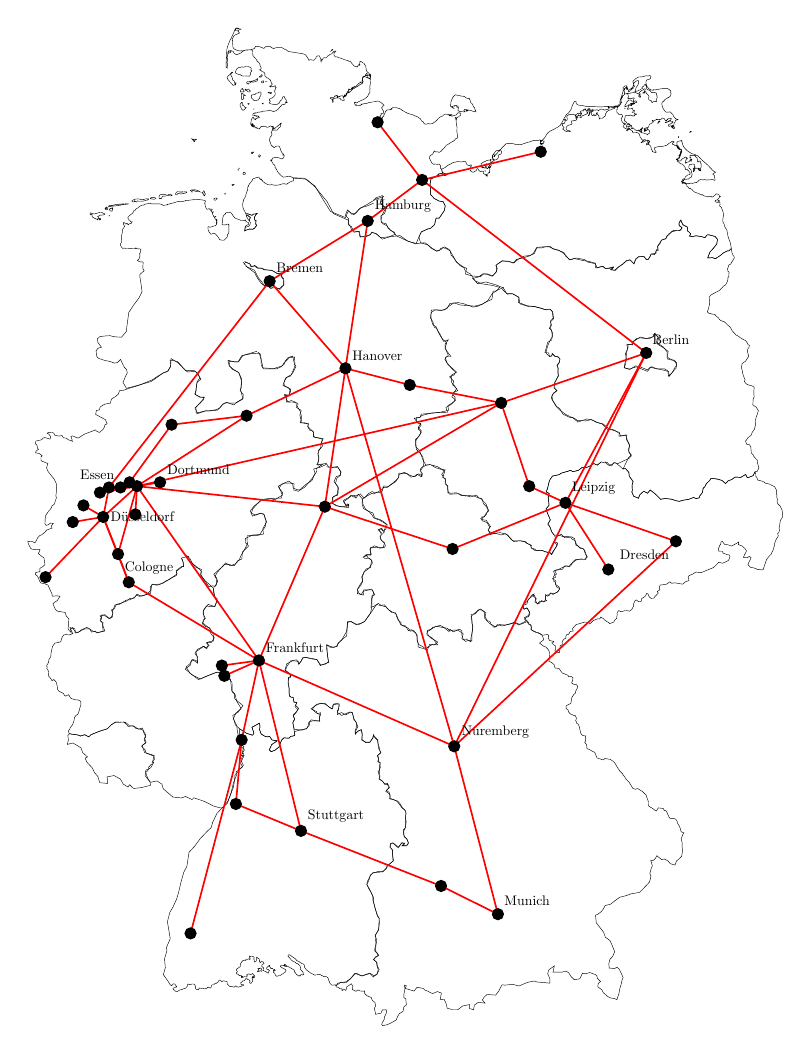
\begin{tikzpicture}

\definecolor{darkgray176}{RGB}{176,176,176}

\begin{axis}[
hide x axis,
hide y axis,
tick align=outside,
tick pos=left,
x grid style={darkgray176},
xmin=5.41798591613775, xmax=15.4935913085937,
xtick style={color=black},
y grid style={darkgray176},
ymin=46.8806100845338, ymax=55.4458555221558,
ytick style={color=black},
width=\linewidth,
height=1.28\linewidth
]
\addplot [line width=0.16pt, black]
table {%
8.70837306976324 47.7155570983886
8.71268272399902 47.7060623168946
8.71873188018799 47.6989135742188
8.71139812469477 47.6942787170411
8.69994831085216 47.6980361938477
8.69212532043457 47.6993370056152
8.68490028381348 47.6944847106934
8.67888832092291 47.6914443969727
8.66709423065197 47.6902580261231
8.66470623016357 47.6931343078614
8.66127586364757 47.6956634521484
8.66714191436779 47.6972236633302
8.67325878143305 47.6996383666992
8.67633533477795 47.705909729004
8.67048358917236 47.7113990783691
8.66622734069836 47.7148742675782
8.67177963256836 47.7169189453126
8.68023490905762 47.7178802490236
8.68641281127941 47.7136421203613
8.69133853912354 47.7165451049806
8.7006978988648 47.720142364502
8.70837306976324 47.7155570983886
};
\addplot [line width=0.16pt, black]
table {%
9.65046024322515 49.7763404846192
9.64671993255615 49.7352600097657
9.63594913482672 49.723991394043
9.63150024414062 49.6978416442872
9.68196868896479 49.7130584716797
9.734221458435 49.6947593688966
9.79042911529547 49.7175102233886
9.81357955932623 49.7102394104005
9.83292961120611 49.6546211242676
9.86216926574713 49.6362915039064
9.863450050354 49.6029090881348
9.84764003753668 49.5694007873536
9.84862041473389 49.5434799194336
9.88179874420172 49.5697097778321
9.92138957977306 49.5774688720703
9.93358993530279 49.5553703308107
9.9292192459107 49.5183410644531
9.92999839782721 49.4961585998536
9.98171043396007 49.4818916320802
10.0272397994996 49.4823112487794
10.0602989196777 49.5158119201661
10.0708284378052 49.5417518615723
10.0829687118531 49.5196914672852
10.1178789138795 49.4978485107423
10.1304388046265 49.4611091613771
10.1426296234131 49.4354286193848
10.1551504135133 49.3987312316896
10.1159391403199 49.3762817382813
10.1338491439819 49.3470115661622
10.1229391098022 49.3285102844239
10.1516275405884 49.3214416503906
10.1525583267212 49.2846908569336
10.1360483169556 49.2588005065918
10.1419305801392 49.2515106201172
10.1484308242798 49.2148399353028
10.1430997848511 49.1964187622071
10.1835393905641 49.1748085021974
10.2068395614625 49.1530303955078
10.2411603927612 49.1533889770509
10.2531890869142 49.1241607666016
10.2192888259888 49.0981292724609
10.2597303390504 49.0802116394044
10.2715091705323 49.0620002746582
10.271809577942 49.0436820983887
10.3179388046265 49.0331687927246
10.3584299087525 49.0189399719239
10.3934898376466 48.9899787902833
10.4167490005493 48.9682197570801
10.4391298294067 48.9606819152832
10.4558286666871 48.9457702636719
10.4669189453125 48.9272117614747
10.4555187225343 48.8977584838868
10.4665498733522 48.8644218444825
10.4607086181642 48.8238410949708
10.4493999481202 48.8091697692872
10.4437198638917 48.7981414794922
10.4323701858521 48.7760810852051
10.4378900527954 48.7575607299805
10.4490718841552 48.7426719665527
10.4770889282227 48.7239418029786
10.4938383102417 48.6941986083985
10.4712591171265 48.672248840332
10.4318799972534 48.6726303100586
10.4488496780395 48.6946296691895
10.4094686508179 48.6950187683105
10.3698692321777 48.6584815979004
10.3020696640015 48.6958007812501
10.2734708786012 48.6883697509767
10.2792100906373 48.6590385437012
10.301968574524 48.6369400024414
10.3018493652345 48.5963897705079
10.3073301315308 48.555690765381
10.2505998611451 48.5231018066407
10.2335996627809 48.5157890319825
10.2225599288942 48.4969596862794
10.1835803985596 48.4701118469238
10.1218395233155 48.4724998474122
10.0602903366089 48.4601097106934
10.0324802398682 48.4410095214843
9.99945068359381 48.3995895385743
9.98865890502935 48.3734092712402
10.011589050293 48.3403892517091
10.0457096099855 48.303810119629
10.0685291290284 48.2706718444825
10.0689191818237 48.2408599853516
10.0919904708862 48.1777496337892
10.1203107833863 48.1295204162598
10.1427507400513 48.1035804748536
10.1429491043091 48.0811614990234
10.1324081420899 48.0175285339355
10.0884895324708 47.9722709655763
10.110899925232 47.9388694763185
10.1001195907593 47.9014015197754
10.0948390960694 47.8639602661133
10.0949506759645 47.8452796936035
10.1060085296631 47.8416404724121
10.1281871795655 47.8156509399414
10.0951404571534 47.8078689575196
10.0731897354125 47.7852210998535
10.111780166626 47.7630691528321
10.1173086166382 47.7368392944336
10.1394691467285 47.7070999145508
10.1118392944337 47.6692314147949
10.0785303115844 47.6573905944824
10.0730514526367 47.6611213684083
10.0240898132324 47.6799316406251
9.97525978088385 47.6687393188477
9.92632865905762 47.6574096679688
9.84401988983154 47.6790313720703
9.81698989868164 47.6564903259277
9.78452968597423 47.6338920593263
9.74108982086193 47.6147994995117
9.70850086212164 47.6031799316406
9.67553997039806 47.6100387573242
9.64301013946533 47.5943489074708
9.61582946777344 47.5823020935059
9.60809707641602 47.5875549316407
9.59931564331055 47.5886344909669
9.59156322479254 47.5874824523926
9.58055114746094 47.5858955383301
9.56746578216564 47.5864715576173
9.55880260467541 47.5887489318848
9.55422782897955 47.591781616211
9.54609680175787 47.5974426269531
9.53862190246582 47.6039581298829
9.53589153289806 47.6126098632814
9.53309917449951 47.6181373596191
9.52856636047369 47.6193656921388
9.52529335021973 47.6254386901856
9.52381896972668 47.629135131836
9.52054023742676 47.6396560668946
9.51149272918713 47.6456222534181
9.50139141082775 47.6514587402344
9.48963165283209 47.6528053283691
9.48559665679932 47.6519966125489
9.4783754348756 47.6528930664062
9.47086143493658 47.651683807373
9.46423339843756 47.6545143127441
9.45750808715826 47.6581802368165
9.44812011718761 47.659523010254
9.43903255462652 47.6610946655273
9.42863941192627 47.6671295166016
9.42107486724848 47.6689834594727
9.4103507995606 47.6703491210938
9.39669227600092 47.6690368652344
9.39076995849609 47.6675834655762
9.3746967315675 47.6669807434082
9.36424160003662 47.6638488769532
9.35340976715088 47.664867401123
9.34339332580572 47.668212890625
9.33466625213634 47.6726226806641
9.32297325134272 47.6757583618165
9.31399726867681 47.6776199340821
9.30723381042486 47.6811218261718
9.29708385467535 47.6851539611817
9.29158020019531 47.689064025879
9.28154468536371 47.6937446594239
9.26723480224615 47.6994667053223
9.25749015808117 47.7048988342285
9.25014114379888 47.7104835510254
9.24290466308588 47.7170372009278
9.23632717132574 47.7226371765137
9.23141384124767 47.7293014526368
9.23014163970942 47.7369461059571
9.23065662384033 47.7432098388672
9.22443294525146 47.7482109069824
9.2136049270631 47.7519302368164
9.20805168151861 47.7532234191895
9.20123672485346 47.7544631958008
9.19145011901861 47.7590599060059
9.18303108215343 47.7624626159669
9.17338562011724 47.7661933898926
9.16315460205089 47.7707443237306
9.15264892578136 47.7739028930665
9.14535617828375 47.7753715515137
9.13589954376221 47.7795181274415
9.13059806823736 47.7854080200196
9.12322807312023 47.7908782958985
9.11534500122082 47.7942619323731
9.10388755798346 47.8007392883301
9.09918880462652 47.8025970458986
9.09108543395996 47.8041038513184
9.08247089385986 47.8089294433594
9.0749311447143 47.8122177124023
9.07011222839355 47.8168601989746
9.05317878723139 47.8216400146486
9.0467987060548 47.8235092163087
9.04012203216547 47.8222045898438
9.03320407867437 47.8167381286622
9.03183364868175 47.8129463195801
9.03997707366943 47.8063850402832
9.04921340942377 47.8014678955079
9.05444812774658 47.7963714599609
9.06152534484875 47.7916717529297
9.06891536712658 47.7852935791016
9.07866191864019 47.779483795166
9.08832454681402 47.7744712829591
9.09452724456787 47.7718505859376
9.1033754348756 47.7694129943848
9.11176872253429 47.7672576904297
9.12090778350841 47.7643127441406
9.12673091888422 47.7603073120117
9.13243103027355 47.7562713623046
9.13851070404064 47.7539863586426
9.15197944641108 47.7531929016113
9.15660190582281 47.7489128112794
9.1696834564209 47.7415885925294
9.17700290679932 47.7377548217775
9.17987060546881 47.7334213256836
9.18145370483398 47.7278709411622
9.18323516845703 47.723014831543
9.18505859375011 47.7189559936523
9.18371582031256 47.7103919982911
9.18822574615479 47.7066345214845
9.19218921661383 47.7022895812989
9.20068073272699 47.6975593566895
9.21247482299799 47.6903038024903
9.21541595458996 47.6844253540039
9.21637821197521 47.6759376525879
9.2215576171875 47.6689567565919
9.21742343902588 47.6667251586915
9.21097278594965 47.6650924682618
9.20100402832031 47.6685295104981
9.18757057189947 47.6692504882814
9.18506145477295 47.6643333435059
9.18147659301763 47.6574096679688
9.17087745666504 47.6605148315431
9.16667747497564 47.6618881225586
9.16502189636242 47.6571922302246
9.15844345092779 47.6579513549805
9.15294647216797 47.6605720520021
9.14853286743175 47.6659393310547
9.13695621490484 47.6681976318359
9.13035774230963 47.672836303711
9.12495899200434 47.6801300048829
9.11803817749035 47.6869888305665
9.11036586761475 47.688461303711
9.10772037506104 47.6919555664064
9.11163139343256 47.6946105957032
9.10950660705566 47.6994132995606
9.10383987426763 47.7048873901368
9.09731960296642 47.7083930969239
9.08959770202642 47.7112808227539
9.08130836486822 47.7134933471681
9.07031917572021 47.7178497314454
9.06135559082031 47.7216835021973
9.05045032501221 47.7261543273926
9.04244804382324 47.7277336120607
9.03370380401617 47.7314605712892
9.02359199523937 47.7336387634278
9.0131950378418 47.7391738891602
9.00182247161865 47.7456588745117
8.99239635467529 47.7479782104493
8.98550701141357 47.7454147338867
8.98817157745373 47.7411727905275
8.99635124206549 47.738452911377
9.0031938552857 47.7357177734375
9.01009559631348 47.731315612793
8.99729061126715 47.7321701049805
8.98511028289789 47.7368774414062
8.97660160064703 47.7398071289063
8.96861362457287 47.7408981323243
8.95772552490246 47.7418823242188
8.95046997070324 47.7406311035156
8.94417381286615 47.7381248474121
8.94136524200445 47.7318229675293
8.94789314270014 47.7273674011232
8.95422363281256 47.7254943847657
8.96321487426758 47.7214126586914
8.97292327880865 47.7169494628907
8.97875118255615 47.7149810791016
8.98491859436035 47.7132148742677
8.99152565002453 47.7115745544434
8.99672508239752 47.7102661132814
9.00337696075445 47.7057037353517
9.00872898101807 47.7000312805176
9.00550270080566 47.6943664550782
8.99800872802729 47.6882476806641
8.99105644226086 47.6840248107911
8.98582363128662 47.6820831298828
8.9809455871582 47.6804008483888
8.9737167358399 47.6746253967286
8.96322441101086 47.6727447509766
8.95596313476568 47.6699180603028
8.94959831237799 47.6669654846191
8.94071388244635 47.661678314209
8.92500972747808 47.6613731384278
8.91370391845697 47.6579627990723
8.90520191192638 47.6567687988281
8.89183425903332 47.6552238464357
8.87854003906256 47.6658515930176
8.87299537658691 47.6762657165527
8.86657619476318 47.6817436218263
8.860016822815 47.6839294433595
8.8548383712768 47.6879997253419
8.85904026031494 47.6944732666015
8.85572910308832 47.6989555358886
8.85916233062738 47.7020797729493
8.86531639099127 47.7003784179689
8.86726093292248 47.6974258422852
8.87013912200939 47.6968231201172
8.87787246704107 47.6989212036133
8.87658691406256 47.7021064758301
8.87370681762707 47.7049293518066
8.87209320068371 47.7085342407228
8.8550767898559 47.7081947326661
8.84860324859625 47.7121810913087
8.84465408325201 47.7162895202638
8.83664035797131 47.7179412841796
8.82831192016613 47.7151031494141
8.82244777679455 47.7168884277344
8.82460021972668 47.7212753295899
8.82076835632319 47.7217826843262
8.81555271148682 47.7270812988282
8.80809402465832 47.7294616699219
8.81241321563721 47.7334556579591
8.81119728088379 47.7357864379883
8.80929374694836 47.740249633789
8.80632114410412 47.7417984008789
8.79995632171642 47.7387847900391
8.79578304290783 47.7325515747071
8.78918266296392 47.7320938110352
8.78331184387207 47.7271347045898
8.77269458770752 47.7218818664551
8.77110385894775 47.7186965942382
8.77216911315918 47.7119445800782
8.78043079376226 47.7097396850585
8.79748630523687 47.7072372436525
8.79992485046398 47.7030181884767
8.80505752563488 47.7002639770508
8.80853271484381 47.6978797912598
8.80264472961431 47.69637298584
8.79735946655279 47.6904220581056
8.79629611968994 47.6814765930176
8.79178714752209 47.6793975830079
8.78179740905773 47.6826667785645
8.77375507354742 47.6864814758301
8.76686096191406 47.6908988952638
8.75304985046381 47.6949806213379
8.73966598510742 47.6966819763184
8.72960376739502 47.7051963806153
8.73334026336664 47.7132644653321
8.73743343353266 47.7203712463379
8.73475837707525 47.7235221862794
8.72563266754162 47.7267379760742
8.71699523925793 47.7299385070801
8.7134313583374 47.7350196838379
8.71482753753668 47.7417640686036
8.71932792663574 47.7455215454102
8.72465801239019 47.7497825622559
8.73334789276123 47.7511138916017
8.74229717254633 47.7527999877931
8.74053764343267 47.7580528259278
8.73138332366943 47.7633056640626
8.72906875610357 47.7671165466309
8.71936130523676 47.7701454162598
8.71004867553722 47.7696342468262
8.70104694366461 47.7657661437988
8.69786643981939 47.7621459960939
8.69301700592052 47.7624855041504
8.68807888031006 47.7706794738769
8.68549633026123 47.7755165100098
8.68839740753174 47.7802963256837
8.68372154235846 47.7855491638183
8.68181514739996 47.7921981811523
8.67188072204596 47.793399810791
8.66308689117426 47.7966003417969
8.66181182861334 47.8009719848633
8.65870666503906 47.8051910400391
8.65114688873291 47.8051300048828
8.64780712127691 47.7999229431152
8.64606094360352 47.7959175109863
8.64925193786632 47.7908935546876
8.64937305450445 47.7808074951172
8.64617824554449 47.7741088867188
8.64328956603998 47.771224975586
8.64021873474127 47.7699737548829
8.63050937652588 47.7657737731934
8.62617301940929 47.7697601318361
8.62173557281494 47.7739295959473
8.62348842620855 47.7819099426271
8.62011241912847 47.7851753234863
8.61669158935558 47.7901153564454
8.61961269378662 47.7944793701172
8.62158775329601 47.8017196655273
8.61474895477295 47.8076362609864
8.60294437408453 47.8091011047364
8.59474372863775 47.8063049316406
8.59028244018566 47.8076667785646
8.58341407775879 47.8077354431152
8.57697010040278 47.8070449829102
8.57386779785156 47.8120498657227
8.5686759948731 47.8143997192384
8.56313991546631 47.8113059997558
8.56232833862305 47.7999725341797
8.56805992126465 47.7970008850097
8.57480812072748 47.7928314208985
8.57164669036877 47.7875518798828
8.56379985809326 47.7875175476074
8.55491924285894 47.7910957336426
8.5483484268189 47.7901306152344
8.53843688964849 47.7880249023438
8.52550315856928 47.7843322753906
8.52108097076422 47.778305053711
8.51064491271978 47.7829437255861
8.50574398040771 47.7810249328613
8.49781322479248 47.7789306640626
8.49124526977545 47.7793998718263
8.48542690277111 47.778175354004
8.47800254821772 47.7733230590821
8.47058391571051 47.7679901123047
8.46823215484619 47.7631912231445
8.46524238586431 47.759693145752
8.45897006988537 47.757610321045
8.45654582977306 47.7513618469239
8.45364570617687 47.7474555969238
8.45261192321789 47.7400283813478
8.45591640472406 47.7332649230958
8.44421100616466 47.727840423584
8.44092559814453 47.7240943908693
8.43522071838379 47.723545074463
8.42614078521734 47.718246459961
8.41727733612055 47.7165603637696
8.4077291488648 47.7081985473634
8.40561485290533 47.7034225463868
8.41038513183594 47.7012672424316
8.41483974456793 47.6950988769531
8.41806221008301 47.690773010254
8.41506671905518 47.6867370605469
8.40631771087641 47.6838836669922
8.40472316741949 47.6787452697753
8.41301155090343 47.6720390319825
8.42396926879894 47.6713371276855
8.43025398254395 47.6682739257813
8.43540000915533 47.6643829345703
8.44223690032959 47.6607704162599
8.45190620422369 47.6595458984376
8.46172237396246 47.6596946716309
8.46718406677246 47.6611022949218
8.4658727645874 47.6533050537109
8.46818065643322 47.6453437805177
8.47563457489025 47.6434135437013
8.47862529754644 47.6453018188477
8.47322654724132 47.6467018127441
8.47423934936529 47.6486663818361
8.47744941711431 47.6503562927246
8.47510719299316 47.6544380187989
8.48215579986572 47.6535263061523
8.48421001434338 47.6495628356933
8.48891162872314 47.6482238769532
8.49495410919184 47.6478042602539
8.49670696258551 47.6515541076661
8.50172328948975 47.6520919799806
8.52180194854748 47.6509819030762
8.53375244140619 47.651035308838
8.53589725494385 47.6544456481934
8.5318603515625 47.6618843078614
8.5327262878418 47.6667861938478
8.53828525543219 47.663917541504
8.54125499725336 47.6647453308106
8.54394912719721 47.6703720092774
8.56136226654064 47.674674987793
8.57065582275396 47.6691246032715
8.57901000976562 47.6675910949708
8.58792495727545 47.6708793640138
8.59741973876964 47.6745796203613
8.60257434844971 47.6769714355469
8.61126804351807 47.6683006286621
8.61979579925537 47.6639213562012
8.62553977966314 47.6598205566406
8.6293888092041 47.6535186767578
8.6250953674317 47.6458625793458
8.61572360992437 47.6416931152344
8.60432529449474 47.64315032959
8.60906410217291 47.6462898254396
8.61533355712902 47.6501846313478
8.61017990112305 47.6560173034669
8.60499000549316 47.6551628112794
8.59684658050548 47.6471939086914
8.59804725646984 47.6345481872559
8.60279464721685 47.6254615783692
8.60586929321295 47.6168937683107
8.59806728363037 47.6113128662109
8.59033775329601 47.6057624816895
8.58634185791027 47.6028289794922
8.58178424835205 47.5997772216797
8.57199287414551 47.6011924743653
8.56536293029791 47.609031677246
8.5719194412232 47.6148300170899
8.57200813293457 47.6178207397461
8.56497573852539 47.6212997436523
8.55906963348389 47.6276054382325
8.54800891876221 47.6295013427734
8.54068088531494 47.631519317627
8.53899097442638 47.6347961425781
8.53183078765881 47.636344909668
8.52302646636969 47.6379623413087
8.51887035369879 47.6365852355956
8.51397514343267 47.6293640136719
8.50899219512945 47.6270828247071
8.50658226013195 47.6221199035645
8.49603366851807 47.6191177368165
8.48259353637695 47.618637084961
8.47723865509033 47.6142082214356
8.47123908996576 47.6092948913575
8.46470355987549 47.6075019836426
8.45824337005615 47.6053199768066
8.45950031280518 47.6011848449708
8.46142673492437 47.5941162109376
8.46748924255382 47.5896759033204
8.47150897979731 47.5885543823243
8.48195743560791 47.5894660949708
8.49204444885254 47.5909423828125
8.48968315124512 47.582763671875
8.47814178466803 47.581356048584
8.47262668609625 47.5788688659669
8.45789909362799 47.5765266418457
8.44715595245361 47.5738372802735
8.43453121185314 47.5713272094727
8.42343139648443 47.5707511901857
8.41617393493664 47.5744094848633
8.40685558319092 47.577709197998
8.39744186401379 47.580150604248
8.38742160797125 47.5745353698731
8.38315677642822 47.5703124999999
8.37329864501964 47.5716209411622
8.35743618011486 47.5742416381837
8.33047389984131 47.5747642517091
8.32132053375244 47.5784606933595
8.31454944610596 47.5834808349609
8.29977798461925 47.5913276672364
8.29470157623297 47.5965003967286
8.29558563232422 47.6082000732422
8.29330921173107 47.6126823425294
8.28142738342297 47.6163368225099
8.27288818359375 47.6161689758302
8.26095867156988 47.6178894042969
8.25420379638672 47.620059967041
8.24035167694092 47.6181640625001
8.23482704162603 47.6162605285645
8.22952365875256 47.6115531921388
8.22291278839117 47.6130638122559
8.21815490722656 47.622573852539
8.2067956924439 47.6262550354005
8.19632816314709 47.6241264343262
8.18986892700201 47.6179962158203
8.18776798248302 47.6148719787598
8.18297386169434 47.6098442077638
8.1759462356568 47.6084938049318
8.17027664184582 47.6041145324708
8.16212463378912 47.5996131896973
8.15146446228022 47.6012763977052
8.14140129089355 47.5982208251953
8.13720417022705 47.5918617248536
8.13370609283453 47.5890541076661
8.11497402191168 47.5892066955567
8.10432720184326 47.5844078063965
8.10028171539307 47.5709686279297
8.09580707550049 47.5655212402345
8.08651161193859 47.5628051757813
8.07672309875494 47.5660247802735
8.0710134506225 47.5700035095216
8.06526947021496 47.569881439209
8.05796813964849 47.5688858032227
8.04987525939953 47.5635643005371
8.03913402557379 47.5593109130859
8.01532363891607 47.5568771362305
8.00687599182135 47.5593643188477
7.9995379447937 47.5624160766602
7.98657608032238 47.5614891052246
7.97047805786133 47.5616455078126
7.9571299552918 47.56400680542
7.95049285888666 47.5555419921876
7.94698715209961 47.5500297546387
7.93535804748541 47.5523071289063
7.91738605499279 47.5539131164551
7.90874481201172 47.5603256225587
7.90722417831415 47.5685386657715
7.91026782989508 47.5759582519532
7.90484380722052 47.5839538574219
7.89448404312134 47.5920257568361
7.88652515411371 47.5948944091798
7.86763381958008 47.5952033996581
7.85302877426147 47.5913429260255
7.84006214141851 47.5888862609864
7.83285522460938 47.5925521850587
7.82077217102056 47.5946998596192
7.81562089920044 47.5909194946289
7.8118138313294 47.5827026367187
7.80856800079346 47.5754699707031
7.80025911331177 47.5706901550294
7.79436206817638 47.5646133422852
7.78735065460205 47.5618591308595
7.77046012878424 47.5591278076172
7.75716018676769 47.5557289123535
7.75042819976801 47.5516777038575
7.72458600997925 47.5497512817383
7.70842981338501 47.5442657470704
7.69653606414795 47.5389595031738
7.68693876266479 47.5361022949219
7.66517782211309 47.538833618164
7.6569390296936 47.5460662841798
7.65017890930176 47.5495491027833
7.64268398284912 47.5519828796387
7.63682699203503 47.5587043762208
7.63945198059076 47.5631065368653
7.64800930023193 47.56498336792
7.66280603408825 47.5679054260255
7.6720399856568 47.5717277526857
7.67832088470459 47.5705413818359
7.68170309066772 47.5735359191895
7.67740488052362 47.5763473510743
7.67208814620966 47.5850105285645
7.66676616668701 47.5863838195802
7.6645069122315 47.5893058776855
7.65889120101934 47.5940628051758
7.64944601058954 47.5961647033691
7.63876819610596 47.5969467163087
7.63531112670898 47.5926742553711
7.62842178344721 47.5879516601563
7.62015104293823 47.5820465087891
7.60277509689337 47.5896835327149
7.57183313369745 47.6214981079102
7.52001142501837 47.6680755615235
7.5438866615296 47.7225837707521
7.53389596939093 47.7902183532715
7.56260490417486 47.853084564209
7.55832004547131 47.8812789916993
7.60334253311157 47.9485626220703
7.56931543350231 48.0806770324707
7.58777141571039 48.1280059814454
7.59949970245361 48.1556320190431
7.63713073730469 48.195873260498
7.68145990371715 48.2596397399903
7.70507860183727 48.3096351623536
7.73096609115606 48.3822059631348
7.76616191864014 48.4639739990235
7.80516195297247 48.5135002136231
7.83175373077404 48.6232795715332
7.8962516784668 48.6672096252442
7.96770238876343 48.7297859191895
8.01622200012213 48.7623977661132
8.05623722076416 48.7896461486816
8.10069656372065 48.8154487609864
8.11810111999506 48.8563079833984
8.16850566864019 48.9245033264161
8.23029518127453 48.9672966003419
8.2952995300293 49.0041503906251
8.3408002853393 49.0840110778809
8.36952018737793 49.1632385253907
8.40528869628912 49.2203521728515
8.40367889404291 49.2499122619629
8.48058891296392 49.289821624756
8.45673084259039 49.3183708190919
8.49954032897961 49.3787803649902
8.46553993225098 49.3775291442872
8.50355815887451 49.4229621887208
8.44516944885254 49.4612503051757
8.44361877441412 49.501579284668
8.44622039794922 49.5861892700195
8.5276603698731 49.5521697998047
8.60262966156006 49.5363311767579
8.61937904357916 49.5515289306641
8.59504890441895 49.5983886718749
8.68616867065435 49.6305313110352
8.69249820709229 49.6087417602539
8.68750858306879 49.5793113708497
8.70555973052984 49.5469322204591
8.74616146087658 49.529811859131
8.78079032897955 49.5234107971192
8.80945873260498 49.527759552002
8.83880996704113 49.4992408752442
8.90242958068853 49.4930992126465
8.86804866790783 49.4779396057128
8.83375930786138 49.4626922607422
8.80581855773926 49.4220085144044
8.82904815673828 49.4079818725587
8.87488937377924 49.4197616577149
8.92646980285656 49.4459686279298
8.93756866455078 49.4716491699219
8.95446014404308 49.4974212646485
8.9830493927002 49.5160217285156
9.04674911499023 49.5128517150878
9.06380844116217 49.527629852295
9.1041898727417 49.5314521789551
9.11559867858898 49.5388298034668
9.10931968688976 49.5645904541017
9.18978977203375 49.5793418884278
9.25874996185303 49.5864486694337
9.27552032470697 49.6085815429688
9.28634071350103 49.6381416320802
9.31462955474865 49.6565589904786
9.41805934906012 49.6452293395996
9.41161823272716 49.6711921691895
9.4280300140382 49.6971321105957
9.39357852935802 49.7045593261719
9.35892868042004 49.7193984985352
9.34142971038824 49.7342185974122
9.31266880035406 49.7416610717773
9.36345958709722 49.767520904541
9.43115901947021 49.7861289978028
9.48233985900879 49.77885055542
9.51671981811523 49.7641105651855
9.56256961822521 49.7420196533203
9.58343982696545 49.7794418334961
9.65565872192388 49.7875595092775
};
\addplot [line width=0.16pt, black]
table {%
10.1338596343995 50.5499992370606
10.175030708313 50.5463218688965
10.2220582962036 50.5388488769532
10.25749874115 50.5127105712891
10.3105001449586 50.4940490722657
10.3458290100097 50.4828720092773
10.3696393966674 50.4418487548828
10.3815002441407 50.4269409179687
10.3933992385864 50.4082794189453
10.4287796020508 50.3896713256837
10.4935398101807 50.3711090087891
10.5171899795533 50.3487510681153
10.5583114624024 50.3525505065919
10.5996913909913 50.3190307617188
10.5999088287354 50.2853622436525
10.605890274048 50.2666816711426
10.6177797317505 50.2442588806153
10.6647691726684 50.2294197082521
10.7230186462403 50.1997985839844
10.7518301010132 50.2447204589844
10.8093795776368 50.241310119629
10.8495798110962 50.2638320922853
10.8035392761232 50.2822418212891
10.7690296173095 50.2932815551758
10.7172508239746 50.322940826416
10.7224493026733 50.3526611328126
10.7798700332641 50.3675994873048
10.8199300765991 50.3825187683106
10.8772802352905 50.3937797546387
10.9118385314942 50.3827590942383
10.9868106842042 50.3459205627443
10.9981107711791 50.3644790649415
11.0385084152223 50.3423614501954
11.1132392883301 50.3648986816407
11.1421594619752 50.3501586914063
11.1421003341676 50.3167495727539
11.1596403121949 50.2834587097168
11.1940393447877 50.2872505187988
11.2516689300537 50.2651901245118
11.2518787384034 50.2911415100098
11.2640590667726 50.3320198059083
11.2763004302979 50.3803787231446
11.2649793624878 50.4100494384766
11.2652893066406 50.4397888183594
11.2540006637574 50.4806289672852
11.3007707595826 50.480812072754
11.347978591919 50.5144386291504
11.3831501007081 50.514560699463
11.4180603027344 50.492359161377
11.4175081253052 50.4514503479003
11.4523401260377 50.4254989624024
11.4814081192017 50.4069709777833
11.5165004730225 50.395881652832
11.5514888763429 50.3810615539552
11.5987586975097 50.3997993469238
11.6690998077392 50.3962516784669
11.7279195785524 50.4038391113282
11.763279914856 50.4113807678224
11.781060218811 50.4188995361329
11.8332996368409 50.4041213989258
11.8683385848998 50.4042091369629
11.9332876205445 50.4230957031251
11.9508810043336 50.4051361083985
11.9728994369507 50.40087890625
11.988410949707 50.3786888122559
11.980833053589 50.3621330261232
11.9984741210938 50.3524780273438
12.042724609375 50.337890625
12.0652704238892 50.3379096984864
12.0980758666992 50.3269500732423
12.1192445755005 50.3130340576173
12.1273336410524 50.2997283935546
12.1371698379517 50.2821121215821
12.0858602523804 50.2553520202638
12.1089019775391 50.2439460754395
12.1319217681885 50.2320747375489
12.161280632019 50.2252082824708
12.1852025985718 50.2088623046876
12.1989192962646 50.1956214904786
12.2102556228639 50.171459197998
12.1990604400635 50.1118202209473
12.2236337661744 50.1068382263184
12.2387990951538 50.1005210876465
12.2619924545289 50.087646484375
12.2671489715576 50.074031829834
12.2734403610229 50.0612945556642
12.3019199371339 50.058864593506
12.3234615325928 50.0559158325196
12.3403053283693 50.0390205383301
12.3644390106201 50.0203819274903
12.3873596191406 50.0163803100587
12.4103908538818 50.0084609985353
12.4300937652589 50.0047760009766
12.4392223358154 49.9918441772462
12.4683113098146 49.9958801269531
12.4915103912355 49.9839515686036
12.4858713150024 49.9634895324708
12.474949836731 49.9445724487304
12.4975881576538 49.9344406127931
12.5331840515136 49.930633544922
12.5491809844971 49.9181823730469
12.5444335937501 49.9042472839355
12.526593208313 49.8848419189454
12.5192785263063 49.8639907836915
12.5033111572267 49.8559761047363
12.4783086776733 49.8320312500001
12.4698915481567 49.8037109375001
12.4658308029174 49.7857551574708
12.4473314285279 49.779411315918
12.4087495803834 49.7661895751954
12.4084739685059 49.7448501586915
12.4312286376953 49.7328186035157
12.4406900405884 49.7154693603517
12.4583139419557 49.7031402587891
12.4862108230591 49.6961135864258
12.4951152801514 49.6907997131347
12.516598701477 49.6916007995605
12.5329446792603 49.6718978881837
12.5283613204957 49.6570854187012
12.5227203369141 49.6488914489746
12.5303115844727 49.6449050903321
12.536660194397 49.6285514831544
12.5528450012207 49.6246528625488
12.55885887146 49.6174087524415
12.5703268051148 49.5979232788087
12.5753774642945 49.5801544189454
12.5844507217407 49.5536079406739
12.5942611694337 49.5408020019531
12.6154766082764 49.5331649780273
12.6458301544191 49.5310592651367
12.6443939208985 49.4944534301758
12.6328067779542 49.4800148010255
12.6467456817628 49.471939086914
12.6570024490356 49.4582099914551
12.6610746383668 49.4321670532227
12.6898450851441 49.4251441955566
12.7193031311036 49.4136276245117
12.7555837631226 49.4025840759278
12.7829885482788 49.3591842651368
12.8576192855836 49.3436088562013
12.8767499923707 49.3545112609864
12.9411487579346 49.3486595153809
12.9804162979126 49.3320274353027
13.0011110305786 49.3171577453613
13.0326108932496 49.282730102539
13.0609884262086 49.2558517456055
13.0954179763795 49.2338256835938
13.0999822616577 49.2223091125489
13.1145906448364 49.2165374755859
13.1311626434327 49.1972122192383
13.1542034149171 49.1806259155275
13.1691198349 49.1725578308107
13.1861791610718 49.1554489135743
13.2177381515503 49.1211318969728
13.2482128143311 49.1143608093263
13.2749977111816 49.1206436157227
13.3338308334351 49.0973205566407
13.3769292831421 49.0707321166993
13.4074516296388 49.0151824951172
13.4071636199951 48.9933280944824
13.4084062576295 48.9843482971191
13.4374084472656 48.9726219177247
13.4663915634155 48.9608879089355
13.4885816574097 48.9487113952637
13.5033550262451 48.9451217651367
13.5268354415895 48.9692535400391
13.5613679885865 48.9668998718262
13.5891103744508 48.9641113281251
13.5981464385987 48.9477691650392
13.6144990921021 48.9491691589357
13.6252593994141 48.9433708190918
13.634614944458 48.9307212829589
13.6433172225952 48.9167137145997
13.6576251983643 48.8959197998046
13.6675214767456 48.8887939453126
13.697340965271 48.8847885131837
13.72260761261 48.8853912353517
13.736798286438 48.8813133239747
13.7519311904907 48.8700218200685
13.7616329193116 48.847972869873
13.7695722579957 48.8394012451173
13.7775077819825 48.8308258056642
13.7888803482057 48.8169898986818
13.804204940796 48.7826385498047
13.8359575271606 48.7750511169435
13.8235597610474 48.7606811523437
13.8042993545533 48.7282905578614
13.8144683837891 48.7027778625489
13.8162641525269 48.660327911377
13.8200798034668 48.6297721862793
13.8099441528321 48.59090423584
13.7608966827392 48.5613784790039
13.7489957809449 48.5570755004883
13.7286520004272 48.522789001465
13.6723461151123 48.5339279174805
13.6453313827515 48.5543746948242
13.6019525527955 48.5706596374512
13.5657234191895 48.5662689208986
13.5085992813111 48.5963897705079
13.4908790588379 48.5746192932128
13.466835975647 48.5603561401368
13.435447692871 48.5598144531251
13.4545402526856 48.516300201416
13.4411983489991 48.4977531433105
13.4236793518068 48.4577789306642
13.437659263611 48.4363365173339
13.4201545715332 48.3915367126465
13.3686418533325 48.3558235168458
13.297986984253 48.3099098205566
13.1977338790894 48.2989654541016
13.1412687301636 48.2855300903321
13.058403968811 48.2717361450196
13.0034379959107 48.2465362548829
12.9463319778442 48.21732711792
12.8824644088746 48.2075424194337
12.8559894561769 48.1768112182618
12.8324937820435 48.1590919494629
12.7974910736085 48.1415252685548
12.7647256851196 48.1320304870606
12.7737283706666 48.0727195739747
12.8640136718749 47.9982185363769
12.8832569122315 47.960521697998
12.91832447052 47.9440841674805
12.942084312439 47.9312858581543
12.9666528701782 47.8963623046876
12.9973659515381 47.8474273681642
12.971534729004 47.809497833252
12.9376850128173 47.7854537963867
12.9261684417725 47.7532806396484
12.9307203292847 47.7189598083497
12.9976987838746 47.7162590026857
13.023491859436 47.7256660461425
13.05153465271 47.7115440368652
13.0790977478027 47.6757202148438
13.0995168685914 47.6454505920411
13.0879936218263 47.6294746398927
13.076530456543 47.5950012207032
13.0589895248414 47.5579109191895
13.048776626587 47.5206642150879
13.0242395401 47.4727592468262
12.9931430816652 47.4817504882814
12.9473209381104 47.4861221313477
12.9130592346192 47.4967422485352
12.857219696045 47.5283584594727
12.8396644592286 47.5513954162598
12.7920913696288 47.572364807129
12.7970190048219 47.5989112854004
12.8250036239625 47.6143913269044
12.7875633239747 47.6385955810546
12.7791461944581 47.6621894836426
12.756314277649 47.670021057129
12.6943368911743 47.6846656799316
12.6443052291871 47.6741828918457
12.6053342819214 47.6792488098145
12.5741014480591 47.6348838806152
12.5056247711183 47.6290473937989
12.4667396545411 47.6541442871094
12.4402570724487 47.6813812255859
12.4086751937867 47.6962356567383
12.3621530532838 47.6880836486816
12.2970485687257 47.6876602172852
12.2479887008668 47.6875000000001
12.2648983001709 47.7364311218262
12.1988801956177 47.7064285278321
12.1838417053223 47.6771430969239
12.2121057510375 47.6326789855958
12.2092800140381 47.6012001037598
12.1544904708863 47.6053619384767
12.0608491897584 47.6101417541504
12.0168094635009 47.618049621582
11.9396581649781 47.6077308654786
11.8348293304444 47.5792884826661
11.7907781600952 47.5871620178224
11.7553968429565 47.5922279357911
11.6676912307739 47.5862731933595
11.6300992965699 47.5884780883789
11.608759880066 47.5632514953614
11.5926008224488 47.5417556762695
11.5534496307373 47.5084190368652
11.4484786987305 47.5131607055665
11.4125556945802 47.4922332763672
11.3905820846558 47.4707946777344
11.4240808486939 47.4456214904786
11.3416061401367 47.4518241882324
11.2938966751099 47.4301986694337
11.2849788665772 47.3948822021484
11.2355899810791 47.4031791687012
11.2359476089478 47.434196472168
11.1511888504028 47.4235649108887
11.0972509384155 47.3957214355469
11.0232343673707 47.3962020874023
10.9648666381835 47.4060363769532
10.9496288299561 47.4460220336915
10.9265918731689 47.4762153625488
10.8790102005005 47.4740905761719
10.8887186050416 47.5056991577148
10.8941373825074 47.5243263244629
10.845311164856 47.5358276367188
10.7874727249146 47.5203704833984
10.7612400054932 47.5273323059082
10.7269411087036 47.5400238037109
10.6975908279419 47.5456695556642
10.6754474639893 47.5601463317871
10.599970817566 47.5698318481446
10.5791826248169 47.5540237426758
10.5614671707154 47.5397911071778
10.453429222107 47.5610198974609
10.4698295593262 47.5809860229492
10.4459648132324 47.5856666564941
10.4517965316772 47.5575599670411
10.4396677017212 47.5170974731445
10.4384460449219 47.4881553649903
10.4626731872559 47.4797286987305
10.4648036956788 47.4579162597657
10.4700441360474 47.43265914917
10.4349317550659 47.4137001037598
10.4302892684937 47.3823738098145
10.3843297958375 47.3636360168458
10.3621091842652 47.3408699035645
10.3452501296998 47.3139190673829
10.2851896286011 47.2917213439943
10.2363986968995 47.2772216796876
10.1813392639161 47.2699394226075
10.1692867279053 47.2791099548341
10.1761407852174 47.2925491333009
10.2038888931274 47.3231086730958
10.2019653320312 47.3358116149902
10.2262201309204 47.3686408996582
10.2268695831299 47.3929176330567
10.178505897522 47.3934936523437
10.1606607437134 47.3672485351563
10.0961999893189 47.3585090637207
10.0808954238892 47.4045257568361
10.0949831008912 47.4233703613282
10.0886058807373 47.4506454467774
10.0553798675537 47.466869354248
10.0433826446534 47.4893760681152
9.99119472503662 47.5032081604005
9.96118831634516 47.5230407714844
9.96367740631115 47.5411643981935
9.94481468200684 47.5389022827148
9.90803241729742 47.54056930542
9.88100242614757 47.5485458374025
9.85710906982422 47.5382194519043
9.81310176849371 47.5524559020997
9.82004165649414 47.5752944946289
9.8015394210816 47.5971603393556
9.74723911285395 47.5741691589357
9.73667144775402 47.5472412109375
9.73229598999023 47.5453567504883
9.72355270385748 47.5503120422364
9.70933628082275 47.5516967773438
9.70098495483398 47.5486297607422
9.6951141357423 47.5439605712892
9.68802356719971 47.5443000793457
9.68502902984631 47.547721862793
9.68946456909191 47.5498428344728
9.69080257415777 47.5552864074708
9.68641662597656 47.5583343505859
9.67394638061529 47.5574188232422
9.66531181335461 47.5581893920899
9.65615940094 47.5600166320801
9.65301132202154 47.5647773742676
9.64020729064953 47.5679283142089
9.6367712020874 47.5708465576173
9.63286781311035 47.5715637207032
9.62277412414551 47.570915222168
9.61513328552257 47.5761795043946
9.61192798614502 47.5812339782716
9.62124824523926 47.5862388610839
9.63741016387951 47.6017799377442
9.67562007904064 47.6063308715821
9.71927928924561 47.6107521057129
9.74122905731201 47.6073989868165
9.7954092025758 47.637722015381
9.82240962982183 47.660270690918
9.86045074462902 47.6791992187501
9.93178081512451 47.657440185547
9.98069953918468 47.6687507629395
10.0295095443726 47.6761589050294
10.0674896240234 47.6497421264649
10.0895986557007 47.6650619506837
10.1118097305298 47.6729621887208
10.1283702850342 47.7069396972656
10.1117887496948 47.7367897033691
10.1062688827515 47.7667694091796
10.0676794052124 47.7851715087891
10.1006603240967 47.8041801452637
10.1336984634399 47.8194389343262
10.1059894561769 47.8453788757325
10.089409828186 47.8489799499512
10.083830833435 47.8601303100587
10.1000576019287 47.9088706970215
10.0942192077638 47.9499092102052
10.093999862671 47.9760589599609
10.132378578186 48.0212707519531
10.137399673462 48.0811004638671
10.1371698379517 48.1072616577148
10.1147499084473 48.1294593811035
10.0919103622437 48.1852188110353
10.0632390975952 48.2482414245607
10.0628490447998 48.2780303955079
10.0400190353395 48.311149597168
10.011480331421 48.3478202819825
9.98871994018566 48.3697013854981
10.0161504745483 48.4073295593263
10.0324296951295 48.4447288513183
10.0658416748047 48.4639205932617
10.1275291442872 48.4652099609376
10.1835393905641 48.4738197326661
10.2281589508057 48.4970588684082
10.2392406463624 48.5158500671388
10.2562789916992 48.5267295837403
10.3129796981812 48.5556297302247
10.3018903732301 48.6074600219727
10.3019781112672 48.6406211853027
10.2677593231202 48.6626586914062
10.2791976928711 48.6920700073242
10.3077697753906 48.6958007812501
10.3755283355712 48.662109375
10.4151096343995 48.6986618041993
10.4432096481324 48.690990447998
10.4149894714356 48.6728019714357
10.4825496673585 48.6795310974121
10.4938497543336 48.6978912353517
10.4715013504029 48.7313690185547
10.443440437317 48.7427101135254
10.4379081726075 48.7612495422364
10.4379787445069 48.7760314941407
10.4324893951417 48.7982521057129
10.4550285339356 48.8091201782228
10.4607696533203 48.8349189758302
10.4609394073487 48.8644714355469
10.4555492401122 48.9014587402344
10.4557399749755 48.9309997558595
10.4558382034302 48.9494590759277
10.4335298538209 48.9607200622559
10.4167718887329 48.975570678711
10.3932991027833 49.0009803771973
10.3641099929811 49.0226593017579
10.312189102173 49.0331115722656
10.2661209106446 49.0399513244629
10.2713899612427 49.0693397521974
10.2595386505128 49.0912094116212
10.2249002456665 49.1055221557618
10.2645597457885 49.1279411315917
10.241008758545 49.1607208251953
10.2067699432374 49.1567001342773
10.1777496337891 49.1784210205078
10.1374588012695 49.1926918029786
10.1427192687988 49.214771270752
10.1247301101685 49.2550086975098
10.1417598724366 49.2588500976564
10.1409692764282 49.2919197082521
10.1515302658082 49.3251190185547
10.1228504180908 49.3321914672852
10.1336507797241 49.3543701171876
10.1215295791627 49.3800086975098
10.1608381271362 49.398780822754
10.1312484741212 49.4353294372559
10.1246318817138 49.4647407531739
10.1235790252686 49.4979019165039
10.0885486602783 49.5234298706054
10.0710792541504 49.5343589782716
10.0660009384156 49.5158615112305
10.0216703414918 49.4785690307618
9.97614860534674 49.478141784668
9.92974090576166 49.5035514831543
9.93437862396246 49.5331802368164
9.92776012420654 49.5590209960938
9.92124938964849 49.5811805725098
9.87067890167248 49.5621910095216
9.84847831726074 49.5471801757813
9.85333061218267 49.569450378418
9.88053894042963 49.6030616760253
9.85631942749029 49.6399612426759
9.83248996734613 49.6657600402833
9.8134298324585 49.7139587402345
9.7847194671632 49.7174720764161
9.72245979309076 49.7021217346191
9.68297863006603 49.6907005310059
9.63645935058594 49.7127990722657
9.63018035888678 49.7276687622071
9.64653968811029 49.7389907836914
9.65614891052257 49.7763710021973
9.58359909057629 49.775718688965
9.57377910614014 49.742099761963
9.52826023101801 49.7567405700685
9.48785972595221 49.7825813293457
9.4481601715089 49.7861709594727
9.38025856018078 49.7786407470703
9.32418823242188 49.7379417419434
9.34150981903082 49.7305297851564
9.37596988677984 49.7230911254884
9.3878698348999 49.7045593261719
9.42761993408209 49.7119598388672
9.41152000427246 49.6748886108398
9.41795921325678 49.648941040039
9.32625961303717 49.6491203308106
9.29208946228027 49.6381187438966
9.29259872436518 49.6159210205079
9.25866985321045 49.5901489257814
9.20138835906977 49.5755920410157
9.10894870758062 49.5830001831055
9.09056091308594 49.638069152832
9.11314868927002 49.663990020752
9.095290184021 49.6932792663574
9.12947940826416 49.715660095215
9.16348934173595 49.7453804016113
9.12269878387457 49.7708511352539
9.13959026336664 49.793140411377
9.10496044158941 49.7964401245117
9.09277820587158 49.8330993652344
9.06967926025402 49.8327713012696
9.05212974548334 49.8435592651368
9.04594039917004 49.865550994873
9.0451192855835 49.9097213745117
9.03853988647455 49.9501304626465
9.03779888153076 49.9869613647461
9.0667295455932 49.9948387145996
9.04866981506353 50.020320892334
8.99534988403326 50.0451011657715
9.01706981658941 50.0933685302734
9.08629035949713 50.1167907714845
9.15641021728521 50.1144485473633
9.16390991210949 50.0886993408204
9.19011974334728 50.1151008605958
9.21074867248535 50.1414108276367
9.25472927093506 50.1420822143555
9.3270692825318 50.1354217529297
9.38334083557123 50.1247901916504
9.43019962310802 50.0841522216798
9.49134922027594 50.0922393798828
9.52411937713617 50.1112403869629
9.50975990295422 50.1709213256837
9.5018396377564 50.2119789123536
9.50574874877935 50.2419319152833
9.54083824157715 50.2235412597657
9.58082962036133 50.2201499938965
9.63168907165533 50.2317810058595
9.64205932617199 50.2542686462402
9.6813898086549 50.2770004272462
9.74269866943359 50.3446617126465
9.75262928009045 50.4013519287111
9.75783920288086 50.4240913391114
9.80528926849371 50.4205894470215
9.86490917205822 50.4021797180176
9.91777992248529 50.4100494384766
9.96456813812267 50.425350189209
10.0109100341797 50.4668998718261
10.0400190353395 50.4933319091797
10.0985202789307 50.5498886108399
10.1220407485962 50.5574798583985
};
\addplot [line width=0.16pt, black]
table {%
13.1778898239136 52.3903198242189
13.1116189956665 52.4060821533204
13.131049156189 52.4354515075685
13.1387586593628 52.4761199951172
13.1280698776245 52.5133399963379
13.1606092453003 52.5647811889649
13.1554203033448 52.5871009826661
13.2162094116212 52.5825195312501
13.2110280990601 52.6048393249513
13.2671203613282 52.6337013244629
13.3099288940431 52.6367797851564
13.3889493942262 52.6319198608399
13.4317188262939 52.6349792480469
13.4688987731935 52.6492614746094
13.4819107055665 52.6675987243652
13.5293893814087 52.6409492492676
13.5148601531983 52.5892715454103
13.5924396514894 52.5584487915039
13.6457986831666 52.5316886901856
13.6378307342529 52.491039276123
13.6494197845459 52.4797401428223
13.7031803131104 52.4640808105469
13.7327003479003 52.4487915039062
13.749758720398 52.4262809753419
13.7243490219117 52.4007301330568
13.6986083984376 52.3677711486816
13.6488800048828 52.33890914917
13.6445589065553 52.3760299682618
13.5724582672119 52.3882598876954
13.4940395355225 52.3968620300294
13.4278287887574 52.4089622497558
13.3965196609497 52.3871803283693
13.3064098358155 52.4107208251954
13.2520475387573 52.4189109802246
13.1778898239136 52.3903198242189
};
\addplot [line width=0.16pt, black]
table {%
13.8795080184937 53.5010681152344
13.877610206604 53.4753189086914
13.9195804595947 53.4501190185547
13.9056997299195 53.431869506836
13.9367084503175 53.4276733398438
13.9811191558838 53.4341011047364
14.0438995361328 53.4290084838868
14.0920715332032 53.4195213317871
14.1210422515869 53.4420242309571
14.1400747299195 53.4417114257812
14.2150812149048 53.428997039795
14.2448511123658 53.4063415527344
14.2356176376343 53.3694801330568
14.1928892135621 53.3347053527833
14.1544790267945 53.3082885742188
14.1254091262819 53.2608604431153
14.1826286315919 53.2633819580078
14.22008228302 53.2553100585939
14.2791128158569 53.2800903320314
14.3189849853516 53.3016395568848
14.3644485473633 53.315731048584
14.383360862732 53.3154945373536
14.4036426544191 53.3312606811523
14.4146718978882 53.3305053710937
14.4194898605348 53.3036231994629
14.4366683959961 53.2785797119142
14.4441108703614 53.2744750976562
14.4489364624024 53.2622032165528
14.4469757080078 53.2565307617188
14.4357290267945 53.2514572143555
14.4339761734008 53.2423477172853
14.4135322570801 53.2265472412109
14.4077157974243 53.2141113281251
14.3913402557374 53.208625793457
14.3789186477662 53.204158782959
14.3740854263305 53.1853027343751
14.3671817779542 53.1800270080567
14.3702974319459 53.1579284667969
14.3864736557007 53.1491088867187
14.3812189102173 53.1313972473145
14.3825340270996 53.1150665283204
14.3714685440063 53.1083412170411
14.3704023361207 53.1002578735353
14.3711614608764 53.094596862793
14.3657941818237 53.0787239074708
14.3594961166383 53.0706787109376
14.345703125 53.0529174804688
14.3370170593262 53.047924041748
14.3191986083985 53.0417251586913
14.3116779327394 53.036849975586
14.2999544143678 53.0279808044434
14.2922525405883 53.0230712890625
14.2841176986695 53.0183601379394
14.2771921157836 53.0142860412598
14.2705068588257 53.0084838867189
14.2562665939331 53.0031661987306
14.2353305816651 52.9959945678711
14.2221813201904 52.9923706054688
14.1652574539185 52.9717826843263
14.1549119949341 52.9661254882813
14.1436986923218 52.9521484375
14.1474342346191 52.9252586364747
14.1500921249391 52.907341003418
14.136040687561 52.8655014038086
14.1214036941529 52.8400878906251
14.13827419281 52.8299674987793
14.1571197509766 52.8280410766602
14.1764841079711 52.8229522705078
14.2140712738038 52.8204040527344
14.2226886749268 52.811824798584
14.2361364364623 52.8034973144531
14.2546949386598 52.7954330444337
14.2664279937745 52.7824974060059
14.2815341949463 52.7742500305176
14.3030099868775 52.7681922912598
14.3260164260865 52.762996673584
14.3418741226196 52.7555961608887
14.3665161132813 52.7379837036133
14.3984079360962 52.7215461730958
14.4217691421508 52.6943588256837
14.436050415039 52.6828231811523
14.4570837020875 52.670337677002
14.4657154083252 52.6610145568848
14.4888896942139 52.6538772583008
14.5033798217773 52.6475410461427
14.5235509872438 52.6379356384278
14.5330085754396 52.6355094909669
14.5507392883302 52.6275215148927
14.5671510696412 52.6216468811035
14.5824460983276 52.6178855895996
14.5950746536255 52.6094779968262
14.6073713302613 52.5965423583986
14.6164283752441 52.5834426879883
14.6323041915894 52.5797080993652
14.6266088485718 52.5613746643066
14.6130361557007 52.551685333252
14.6077690124513 52.534824371338
14.6085472106935 52.5286674499512
14.6186885833741 52.5068283081055
14.624041557312 52.493553161621
14.6114587783814 52.4817085266114
14.5860900878907 52.4555587768556
14.5432081222535 52.4374885559083
14.5353088378907 52.4037895202638
14.5459909439087 52.3809204101563
14.5477228164673 52.3679237365724
14.5581426620483 52.3438148498536
14.5674667358398 52.3282775878907
14.5799093246461 52.3108367919921
14.5713186264038 52.297119140625
14.5880393981934 52.2817268371583
14.605938911438 52.2733612060547
14.6285943984986 52.2680969238282
14.6634187698365 52.2633590698242
14.6895904541016 52.2522621154786
14.6852760314941 52.2071075439453
14.6895608901977 52.1776313781738
14.6774291992188 52.1589088439941
14.6741895675659 52.1141090393066
14.7159385681152 52.0956611633301
14.7410097122192 52.0696601867676
14.7282171249389 52.0423431396484
14.7158803939819 52.0210494995118
14.7026586532592 51.9874114990234
14.7058696746827 51.9575805664064
14.6926488876343 51.9239311218261
14.66392993927 51.8975791931153
14.652949333191 51.8765487670898
14.6392097473145 51.8698501586913
14.6117420196534 51.8564529418946
14.59893989563 51.8422737121583
14.5855894088746 51.832576751709
14.5887908935548 51.8237075805664
14.6007680892945 51.8062438964844
14.632830619812 51.8033180236817
14.6494750976562 51.7860832214355
14.652738571167 51.7593917846681
14.6549587249755 51.7412033081055
14.6632661819459 51.7325820922852
14.6787853240968 51.7243156433106
14.6878423690796 51.7094306945801
14.7185096740723 51.689121246338
14.7287797927856 51.6817207336426
14.7323789596558 51.6556396484376
14.7468185424805 51.6221885681152
14.7280797958374 51.5959701538086
14.7006101608278 51.5920791625977
14.6769208908082 51.5620803833008
14.628960609436 51.5496215820312
14.6060991287231 51.5460700988771
14.5870704650879 51.5716896057129
14.527681350708 51.5484008789063
14.4583196640016 51.5513801574708
14.4154291152955 51.5310096740722
14.373390197754 51.5217514038087
14.3419990539551 51.5008201599122
14.2976198196412 51.5254821777344
14.2346591949464 51.5364685058594
14.1649990081787 51.54061126709
14.1522092819214 51.5264015197755
14.1092586517333 51.4990692138671
14.0893001556396 51.4738693237306
14.0709009170533 51.4637298583986
14.0612602233887 51.4296722412109
14.029990196228 51.4043922424316
14.0226097106935 51.3893394470215
13.9876604080201 51.3832397460939
13.9532699584962 51.3917808532714
13.8988990783691 51.3779411315919
13.8392381668091 51.3717422485352
13.7792806625367 51.3617820739747
13.7440271377565 51.3662605285645
13.6855096817018 51.3786392211915
13.6085796356201 51.3838500976564
13.5546398162842 51.3774299621583
13.5087003707886 51.4079818725587
13.4681396484376 51.430950164795
13.4272909164429 51.4501495361329
13.3961191177369 51.4247398376466
13.3490390777589 51.4403190612794
13.2998104095459 51.4114990234376
13.2866392135621 51.3857917785645
13.2275590896607 51.401538848877
13.2050676345826 51.4351501464845
13.2115497589112 51.4461517333985
13.2073202133179 51.4868621826171
13.2205801010132 51.5162315368653
13.1743087768556 51.5575714111329
13.169529914856 51.5872192382812
13.1286897659302 51.6173820495607
13.0984888076782 51.6141319274903
13.168378829956 51.7055587768555
13.1992292404175 51.7235984802247
13.1701908111572 51.7499122619629
13.170937538147 51.7683906555176
13.1783208847045 51.8015785217286
13.1383485794069 51.8576507568359
13.1332101821899 51.8799209594728
13.0482692718506 51.8700103759767
13.0554504394532 51.8995094299316
12.965539932251 51.9192619323731
12.9112787246705 51.9237098693849
12.8462295532228 51.9652900695802
12.7800483703613 51.9772720336914
12.7142086029054 52.0003395080567
12.6532783508301 51.9900207519531
12.5503091812134 51.9913215637207
12.4964599609374 52.0141792297363
12.460078239441 52.0146217346192
12.3698587417603 52.0415687561036
12.3286094665528 52.0864295959472
12.2925796508789 52.1016311645508
12.2452487945557 52.1502494812012
12.2339582443237 52.1836700439453
12.2527885437011 52.2056808471681
12.2959899902343 52.2274208068848
12.2599592208863 52.2463111877441
12.2733297348022 52.2905998229981
12.3113193511963 52.3420295715332
12.3120298385621 52.3679504394532
12.3069496154786 52.4050598144531
12.2952404022217 52.4237022399902
12.3264894485474 52.4492988586426
12.333218574524 52.4714622497559
12.3031692504883 52.4903221130372
12.2727108001709 52.4943504333497
12.2426395416259 52.513198852539
12.2299203872681 52.4948005676269
12.2054691314697 52.4950599670411
12.1939086914064 52.5211219787597
12.1510887145997 52.5215606689454
12.1837701797486 52.6027984619142
12.2332592010498 52.6208305358888
12.2402687072754 52.6541404724122
12.2409687042236 52.6800994873046
12.2231693267823 52.7025489807129
12.2049608230591 52.7101593017579
12.2241487503052 52.7396507263185
12.2187995910646 52.769401550293
12.2500991821289 52.7913589477539
12.2392187118531 52.8434486389161
12.215129852295 52.8622703552247
12.1657390594482 52.8553504943848
12.1351776123048 52.863079071045
12.0861501693727 52.8710098266603
12.0125608444214 52.8828620910645
11.9387598037721 52.8872718811036
11.8283891677858 52.9142990112306
11.8353691101075 52.9551315307617
11.7556085586548 52.9818801879883
11.6876382827759 52.9824714660646
11.645058631897 53.0274696350099
11.5586595535279 53.0505218505859
11.434829711914 53.0738410949708
11.3353004455567 53.059700012207
11.273380279541 53.1011505126954
11.3419094085693 53.1117897033693
11.3981103897095 53.1374320983887
11.4478387832642 53.1333122253419
11.5098381042482 53.1179199218751
11.5536909103395 53.1473617553712
11.5727195739747 53.177001953125
11.5543794631958 53.2032318115236
11.629508972168 53.2361297607422
11.7165794372559 53.2353706359864
11.7660398483276 53.2200317382814
11.8038291931152 53.2494888305664
11.8972797393799 53.263511657715
11.9658498764038 53.2777519226075
12.0097103118896 53.2959594726564
12.0479698181152 53.3403091430665
12.1162586212159 53.3395996093751
12.159969329834 53.3503303527833
12.1972007751465 53.3499298095704
12.2464094161988 53.3344802856446
12.3142585754395 53.3225212097169
12.3632583618165 53.303321838379
12.3998384475709 53.2842597961426
12.4481792449951 53.2464408874513
12.5041589736938 53.2569313049318
12.6148891448975 53.2406387329103
12.6703395843507 53.2361793518066
12.7623901367188 53.2200813293458
12.7672080993652 53.1828117370605
12.8479194641113 53.196590423584
12.8841981887817 53.1774787902832
12.9399585723876 53.1841316223145
12.9772386550903 53.1910285949707
12.9455394744874 53.1691818237305
12.9946794509888 53.1647491455078
13.0387096405029 53.1864089965821
13.089098930359 53.2116813659669
13.1397008895875 53.240650177002
13.1830291748047 53.2436904907228
13.2310209274293 53.2132110595703
13.2510480880738 53.2467460632325
13.2851066589355 53.2693672180175
13.3468122482301 53.2719879150391
13.3822898864747 53.2479248046875
13.4054727554322 53.249885559082
13.4315185546876 53.2769165039062
13.4384202957153 53.2915496826173
13.4814214706421 53.2871093750001
13.5017089843751 53.3203125000001
13.5264883041382 53.3198852539062
13.515685081482 53.3496704101563
13.5544490814209 53.3802413940431
13.5621538162232 53.3990821838379
13.593077659607 53.4062461853028
13.618145942688 53.4108924865722
13.6256942749024 53.4293746948243
13.6572875976562 53.4437255859376
13.6898794174194 53.4652709960938
13.7527084350586 53.4753799438477
13.783839225769 53.4748306274415
13.8165988922119 53.4964904785156
13.7864990234376 53.5119018554688
13.7750854492188 53.5269165039064
13.7936506271363 53.5562171936036
13.8247022628785 53.5221633911134
13.8796291351318 53.5027313232421
};
\addplot [line width=0.16pt, black]
table {%
13.4822502136232 52.6750221252443
13.4626502990723 52.6456413269044
13.4197082519532 52.638858795166
13.3828592300415 52.6319999694824
13.3102483749391 52.6441917419434
13.2730598449707 52.6299018859863
13.210880279541 52.6011390686036
13.2041683197022 52.5863990783691
13.1430807113647 52.5835609436036
13.1543693542482 52.5611610412599
13.1402502059937 52.5131607055665
13.1326808929444 52.4762001037598
13.1185894012451 52.4281997680664
13.1175594329835 52.4022789001466
13.1780490875244 52.3940200805664
13.257809638977 52.411418914795
13.3179292678833 52.3957290649414
13.3960399627686 52.3760719299317
13.4401292800904 52.4124908447265
13.5122089385986 52.3965797424316
13.6030693054199 52.3951988220216
13.6506099700928 52.3759422302247
13.6609592437744 52.3387222290039
13.7050113677978 52.3750915527345
13.7424697875977 52.4004402160645
13.7504701614379 52.4411010742187
13.7213201522828 52.4637985229492
13.6910781860352 52.4642715454102
13.6369600296022 52.4725189208986
13.6317682266235 52.4911308288575
13.6334981918336 52.5281715393066
13.5867185592653 52.5659599304199
13.5033798217773 52.6042594909669
13.5234909057618 52.6447410583496
13.4822502136232 52.6750221252443
};
\addplot [line width=0.16pt, black]
table {%
8.50506019592285 53.2328910827638
8.56754875183111 53.215991973877
8.58109855651861 53.1939811706544
8.62401866912853 53.1988105773926
8.66203975677502 53.1810913085938
8.70527076721186 53.1821098327637
8.74306964874279 53.1680488586427
8.82959079742443 53.1661987304688
8.90495872497564 53.1378822326661
8.95998001098633 53.1464195251465
8.9487390518189 53.1238021850586
8.98070907592785 53.0982513427734
8.98299026489269 53.0497398376465
8.93546962738037 53.0152397155762
8.86048030853271 53.0399017333985
8.83047962188721 53.0243721008301
8.78033924102783 53.0419921875001
8.75573062896734 53.0414619445801
8.71166992187511 53.0591506958008
8.66638946533209 53.0991516113281
8.62685012817388 53.1466789245607
8.53830814361584 53.1891098022462
8.48689079284674 53.2286415100098
};
\addplot [line width=0.16pt, black]
table {%
8.53948402404797 53.6062889099122
8.56286430358898 53.6015167236329
8.58555698394781 53.5957679748535
8.59773921966558 53.5942840576171
8.61647319793701 53.6041259765626
8.64192008972168 53.6041870117189
8.64971446990972 53.6031913757324
8.63795566558838 53.5950660705567
8.62431049346924 53.5775032043458
8.6251544952392 53.5673141479493
8.63198661804199 53.5554656982422
8.63544082641607 53.5537643432618
8.63929748535156 53.5542984008789
8.64253234863281 53.5548934936524
8.64405536651617 53.5496063232423
8.64152145385748 53.5363998413087
8.64427280426025 53.5223922729492
8.65213394165039 53.5160179138184
8.64824295043957 53.509822845459
8.64436912536621 53.5090904235841
8.63749122619635 53.5055618286134
8.63144111633312 53.4936599731446
8.6059045791626 53.4842338562012
8.59377098083507 53.4856834411621
8.58675289154047 53.4858894348145
8.58209228515631 53.4863090515137
8.57495403289801 53.4861717224122
8.57060813903814 53.4881439208985
8.56361484527594 53.4856071472169
8.55576324462896 53.4838829040528
8.54093074798595 53.4815826416016
8.53337097167963 53.4804458618164
8.52367496490473 53.4779167175294
8.50578975677496 53.4711799621582
8.51416683197027 53.5051383972168
8.51583290100109 53.5037498474122
8.517499923706 53.5026397705079
8.51972389221191 53.5015258789063
8.52250003814709 53.5018043518067
8.52583217620855 53.5026397705079
8.53361129760754 53.5037498474122
8.53916740417486 53.504581451416
8.54249858856207 53.5056953430175
8.54916572570806 53.5065269470215
8.55360984802246 53.5076370239259
8.55638790130627 53.5090293884278
8.55916690826416 53.5104179382325
8.56194496154791 53.5118064880371
8.56361103057873 53.5137481689454
8.56527709960938 53.5151405334473
8.56749916076666 53.5165290832521
8.56972122192383 53.518196105957
8.57083415985102 53.5201377868653
8.57250022888189 53.5240287780762
8.57361221313482 53.5268058776857
8.57527828216564 53.5345840454101
8.57472229003918 53.5356941223145
8.57583427429211 53.5370826721192
8.57583427429211 53.5395851135255
8.57416629791271 53.5415267944337
8.57027721405029 53.5426406860352
8.56805515289318 53.5462493896484
8.56583309173584 53.5479164123536
8.56437778472906 53.5598258972169
8.57491588592535 53.5752601623536
8.57550907135021 53.5786056518556
8.5632781982423 53.5812644958496
8.54136276245123 53.596118927002
8.52694416046148 53.5934715270996
8.52694416046148 53.5943069458008
8.527500152588 53.5956954956055
8.52527809143066 53.5968055725099
8.5247220993042 53.5990295410157
8.52250003814709 53.6023597717286
8.52194404602062 53.6056938171387
8.52615928649908 53.6038398742676
};
\addplot [line width=0.16pt, black]
table {%
8.64723300933849 53.6100273132324
8.66088390350342 53.6070861816406
8.65196514129644 53.6039352416993
8.64383220672619 53.6079025268555
};
\addplot [line width=0.16pt, black]
table {%
10.071617126465 53.718231201172
10.1289100646974 53.7258186340332
10.1921787261963 53.7407722473145
10.1612596511841 53.7148513793945
10.1495790481567 53.6852912902833
10.2014694213868 53.6633186340333
10.2215585708619 53.6375617980958
10.2036504745483 53.6079902648926
10.1596193313599 53.5894012451172
10.1613397598267 53.5451316833497
10.1876802444459 53.5267906188965
10.2331104278564 53.5122108459473
10.2466802597047 53.4938316345216
10.3118991851807 53.4608917236329
10.3312196731567 53.4462203979493
10.2676181793213 53.4272308349609
10.1577796936035 53.4189987182617
10.099220275879 53.4521293640137
10.0538988113403 53.4592819213867
10.0218000411987 53.4404487609864
9.97661972045898 53.43270111084
9.90592765808111 53.4247207641601
9.89241981506348 53.4657020568848
9.80922889709484 53.4724617004396
9.78915023803717 53.505989074707
9.76294040679932 53.5319595336914
9.76863956451416 53.5655403137208
9.72939968109142 53.5947494506837
9.75389862060547 53.6353797912599
9.78632926940918 53.6172904968262
9.83185863494879 53.5990715026856
9.88217067718517 53.6325416564941
9.90725898742687 53.6511001586915
9.99017906188965 53.6662406921388
10.072678565979 53.6887092590333
};
\addplot [line width=0.16pt, black]
table {%
9.49876976013195 51.6315193176271
9.56927967071539 51.6253700256349
9.63402080535889 51.6337585449219
9.67084884643555 51.593879699707
9.67166996002209 51.5644989013672
9.61868000030523 51.5563392639161
9.59066009521484 51.5154495239259
9.63875007629395 51.4758491516114
9.63434028625483 51.4278907775879
9.63489818573009 51.4094505310059
9.58295917510986 51.4008407592773
9.5723695755006 51.3746185302735
9.56169891357428 51.3520622253419
9.61463928222651 51.3274002075195
9.66687011718761 51.3213615417482
9.7655286788941 51.3129005432129
9.77073860168457 51.3388900756836
9.74192905426025 51.3234596252443
9.7061386108399 51.3594703674317
9.75267887115484 51.3787498474122
9.80111980438232 51.4045600891113
9.83792972564703 51.4083518981935
9.85679912567139 51.3864097595216
9.8868408203125 51.4159317016602
9.93714809417719 51.3791999816895
9.93114852905285 51.3421211242676
9.94935989379883 51.3048896789551
10.0034799575806 51.2859992980958
10.063398361206 51.2707901000977
10.0756597518921 51.2447395324707
10.0937500000001 51.2297821044922
10.1415195465088 51.2220687866212
10.1952486038209 51.20320892334
10.2251806259155 51.1845016479493
10.2078571319581 51.1475105285645
10.1964292526246 51.1142005920411
10.1721696853638 51.1514205932617
10.1247186660767 51.1405715942383
10.160719871521 51.1181106567384
10.1610183715821 51.0958518981934
10.1494789123536 51.0699615478516
10.1914291381835 51.0437698364259
10.2155103683473 51.0176887512208
10.2038593292237 51.0029106140137
10.1505298614502 50.9957809448242
10.1087598800659 51.0034217834474
10.0311994552613 51.0001602172852
10.0317888259888 50.9630584716798
10.0321493148803 50.9407997131348
9.99024963378906 50.9446601867677
9.95464992523205 50.9298706054689
9.99036979675293 50.937240600586
10.0025682449341 50.9223709106446
10.0447101593018 50.9036521911622
10.0570306777954 50.8813285827638
10.0276393890381 50.8518218994141
9.99801921844488 50.8297119140626
9.95634078979487 50.8113021850586
9.93873023986828 50.7780113220215
9.93893909454351 50.7411003112794
9.90320873260504 50.7078895568848
9.8794288635255 50.6783905029297
9.87310886383051 50.6418418884277
9.92153835296631 50.6341400146484
9.94550991058361 50.6598815917969
10.0489807128906 50.6772613525391
10.0737495422364 50.647331237793
10.0619096755981 50.6288986206056
10.0508108139039 50.5949096679688
10.051329612732 50.5422401428222
10.0341691970826 50.4895515441896
9.99925899505621 50.4593391418457
9.95875930786138 50.4215621948243
9.90029907226568 50.4024314880371
9.85912036895752 50.3983802795411
9.79927921295177 50.4243316650391
9.7521800994873 50.4164886474609
9.75314044952398 50.3861885070802
9.74408912658697 50.3110504150391
9.66998958587646 50.2731704711915
9.63650035858154 50.2504997253419
9.6204185485841 50.2279510498048
9.58063888549805 50.2238922119141
9.54041862487793 50.2310218811035
9.5000896453858 50.2418785095215
9.50769138336182 50.2082901000977
9.50995826721203 50.1671791076661
9.52449035644531 50.1037712097168
9.48556900024425 50.0959205627441
9.42481899261486 50.0803489685059
9.3831291198731 50.1285285949708
9.31619071960455 50.1315689086915
9.24908828735363 50.1457290649415
9.21095752716076 50.1376991271972
9.19033908843994 50.1113891601563
9.16369819641119 50.0923919677734
9.13838768005371 50.125171661377
9.0628986358642 50.1163520812988
9.01789093017578 50.0713005065919
9.0013103485108 50.0415496826172
9.05467987060547 50.0130615234375
9.06680965423595 49.9911499023438
9.03796100616466 49.979591369629
9.0328187942506 49.9463500976562
9.04525756835949 49.9023590087891
9.04600811004639 49.8618698120118
9.05219841003424 49.8398818969727
9.07545852661138 49.8328590393068
9.09862041473389 49.8294906616212
9.10502910614025 49.7927513122559
9.1396598815918 49.7894401550293
9.11713981628429 49.7597503662109
9.15210914611828 49.7379302978516
9.12955856323242 49.7119789123535
9.09542942047125 49.6859321594239
9.11322021484375 49.6603088378907
9.09062862396252 49.6343917846681
9.10931968688976 49.5645904541017
9.11559867858898 49.5388298034668
9.1041898727417 49.5314521789551
9.06380844116217 49.527629852295
9.04674911499023 49.5128517150878
8.9830493927002 49.5160217285156
8.95446014404308 49.4974212646485
8.93756866455078 49.4716491699219
8.92646980285656 49.4459686279298
8.87488937377924 49.4197616577149
8.82904815673828 49.4079818725587
8.80581855773926 49.4220085144044
8.83375930786138 49.4626922607422
8.86804866790783 49.4779396057128
8.90242958068853 49.4930992126465
8.83880996704113 49.4992408752442
8.80945873260498 49.527759552002
8.78079032897955 49.5234107971192
8.74616146087658 49.529811859131
8.70555973052984 49.5469322204591
8.68750858306879 49.5793113708497
8.69249820709229 49.6087417602539
8.68616867065435 49.6305313110352
8.59504890441895 49.5983886718749
8.61937904357916 49.5515289306641
8.60262966156006 49.5363311767579
8.5276603698731 49.5521697998047
8.44622039794922 49.5861892700195
8.39341926574701 49.6175498962403
8.36192989349365 49.6901702880859
8.43006038665777 49.7181396484376
8.48609066009521 49.7677688598632
8.38613891601562 49.8200302124023
8.38475990295416 49.8605995178223
8.34920978546154 49.8853912353517
8.33472919464123 49.9737510681153
8.23441028594965 50.0301017761232
8.14766883850103 50.0238494873047
8.04994869232183 49.9987716674805
7.94610023498547 49.9708518981934
7.84487915039062 50.0194396972657
7.79623985290533 50.0681800842286
7.8420209884643 50.0946693420411
7.86995792388922 50.1285705566407
7.91117906570435 50.1212310791016
7.93498897552502 50.110019683838
7.92744016647339 50.1551399230958
7.91437005996715 50.1887207031249
7.96050786972046 50.2078590393068
8.01224040985113 50.2308616638184
8.04792022705089 50.2125396728517
8.06429958343517 50.2427787780763
8.05195045471203 50.2613487243652
8.09869861602789 50.2583389282226
8.13809013366711 50.2965087890625
8.09609889984137 50.3294410705566
8.08279991149897 50.3741607666016
8.03456878662121 50.3846588134766
7.99076795578014 50.4062805175782
8.0066289901734 50.4364891052247
8.0300083160401 50.4481811523438
8.00260925292969 50.4848899841309
8.01169967651373 50.5186920166015
8.04552936553961 50.5456886291504
8.08928012847906 50.5391921997071
8.13426971435553 50.5395889282227
8.15596008300781 50.5549201965333
8.17358875274658 50.6002616882324
8.14660930633556 50.6154289245607
8.12641811370855 50.65731048584
8.13341045379644 50.6914901733398
8.16411972045904 50.7096519470216
8.16455936431885 50.7584190368653
8.1451997756958 50.7733116149903
8.17286014556896 50.8067817687989
8.2300176620484 50.8477287292481
8.26449966430675 50.8700599670411
8.30697822570812 50.8700218200684
8.3805103302002 50.8589515686036
8.41931915283197 50.8962707519532
8.47149085998535 50.9115219116212
8.47972965240484 50.9669914245607
8.55467891693127 51.0132293701173
8.51747035980236 51.0386619567872
8.5153694152832 51.0723114013672
8.60994815826416 51.1002502441406
8.69318866729736 51.1019210815431
8.71008872985851 51.1246604919434
8.75617980957031 51.1629295349121
8.76619911193853 51.2116889953614
8.74653911590576 51.2523918151855
8.70958137512213 51.2703590393067
8.64383029937738 51.254119873047
8.58795928955078 51.2679595947266
8.60409069061285 51.3019104003906
8.65686035156256 51.3403396606446
8.69834041595453 51.3635711669922
8.76486968994152 51.3760490417481
8.85554981231695 51.3852500915528
8.95163822174084 51.3871421813966
8.96854972839367 51.4285392761232
8.92536926269531 51.4650192260743
8.95466136932379 51.4954490661622
9.04188060760504 51.5192985534669
9.08891963958752 51.497901916504
9.09583854675293 51.4645805358888
9.15401935577393 51.4508209228516
9.18285942077642 51.4513893127442
9.23400974273682 51.4709701538087
9.27875995635986 51.5052604675292
9.32909965515137 51.5433197021484
9.36213970184338 51.5809516906739
9.34346961975092 51.6137619018555
9.43502044677734 51.6303405761719
9.5037088394165 51.653678894043
};
\addplot [line width=0.16pt, black]
table {%
14.2647228240966 53.710693359375
14.266944885254 53.7081947326661
14.2686109542848 53.7070846557618
14.2652769088745 53.7051391601562
14.2625007629395 53.7040290832521
14.2580566406251 53.7031936645507
14.2563877105714 53.7015266418458
14.2519435882568 53.7018051147462
14.2497215270997 53.7031936645507
14.2486124038696 53.7068061828614
14.2502784729004 53.7084732055665
14.2597227096558 53.7087516784669
14.261944770813 53.7101402282716
};
\addplot [line width=0.16pt, black]
table {%
11.4280557632446 53.9431953430177
11.4274997711182 53.9387512207031
11.4247217178346 53.9406929016114
11.4230556488038 53.9423599243165
11.4252777099611 53.9420852661133
11.4274997711182 53.9431953430177
};
\addplot [line width=0.16pt, black]
table {%
13.9597215652466 53.9434738159181
13.960277557373 53.9412498474122
13.9575004577637 53.9409713745118
};
\addplot [line width=0.16pt, black]
table {%
14.0341663360597 53.9465293884277
14.0336122512818 53.9440269470215
14.0319433212281 53.9462509155273
};
\addplot [line width=0.16pt, black]
table {%
14.0236110687257 53.9520835876465
14.0280551910402 53.9504165649414
14.0280551910402 53.9470825195313
14.0258331298828 53.9484710693359
14.0236110687257 53.9493064880372
14.0230569839478 53.9520835876465
};
\addplot [line width=0.16pt, black]
table {%
11.4697208404542 53.9679183959962
11.4691667556763 53.9656944274903
11.466944694519 53.96541595459
};
\addplot [line width=0.16pt, black]
table {%
13.929165840149 54.0312499999999
13.9319438934326 54.0304183959962
13.9336099624634 54.0284729003907
13.93416595459 54.0259704589844
13.9319438934326 54.0245819091796
13.9269437789918 54.0234718322754
13.9258337020874 54.0201377868652
13.9269437789918 54.0156936645508
13.9219455718995 54.016529083252
13.9197225570679 54.0176391601563
13.917498588562 54.0190277099611
13.9158334732056 54.0218048095704
13.917498588562 54.0243072509766
13.9191665649414 54.0259704589844
13.9213886260987 54.0270843505859
13.9230546951295 54.0290260314943
13.9258337020874 54.0301399230958
13.9286098480226 54.0309715270996
};
\addplot [line width=0.16pt, black]
table {%
11.4958333969116 54.0318069458009
11.4980554580688 54.0306930541992
11.496389389038 54.0290260314943
11.4921016693116 54.0245819091796
11.4891672134401 54.0240287780762
11.4869441986085 54.0262489318848
11.4902763366699 54.0284729003907
11.4919452667236 54.0301399230958
11.4941673278809 54.0309715270996
};
\addplot [line width=0.16pt, black]
table {%
11.5236110687257 54.0695838928223
11.5230550765992 54.0679168701172
11.5208330154419 54.0640258789064
11.5180568695069 54.062084197998
11.5163888931275 54.0562515258788
11.5163888931275 54.0509719848633
11.5173778533935 54.048194885254
11.5158319473267 54.0431938171387
11.5147218704224 54.0390281677246
11.5136098861694 54.0381927490234
11.5108337402344 54.0451393127441
11.5113878250123 54.0510368347168
11.5130558013917 54.057918548584
11.5147218704224 54.0601387023927
11.516944885254 54.0626373291016
11.5186109542848 54.0643043518068
11.520278930664 54.067081451416
11.5230550765992 54.0690269470215
};
\addplot [line width=0.16pt, black]
table {%
13.7686100006104 54.1265258789063
13.7702779769898 54.1215286254883
13.7725000381469 54.1195831298828
13.7741661071777 54.1168060302735
13.7786111831664 54.1159706115723
13.7813892364503 54.1145820617676
13.7836112976075 54.1129150390625
13.7852773666382 54.1109733581544
13.7863893508911 54.1101379394532
13.7825012207032 54.1118049621583
13.77805519104 54.1126403808594
13.7786111831664 54.1109733581544
13.7763891220093 54.1109733581544
13.7758321762086 54.1143074035646
13.7702779769898 54.1165275573731
13.7697219848633 54.1204147338868
13.7680559158325 54.1223602294922
};
\addplot [line width=0.16pt, black]
table {%
13.7636117935181 54.1270828247071
13.7652778625489 54.1251373291016
13.7619457244872 54.1262512207031
};
\addplot [line width=0.16pt, black]
table {%
13.3502769470214 54.1779174804689
13.3519449234009 54.1765289306641
13.3486108779908 54.1762504577637
13.3491668701172 54.1779174804689
};
\addplot [line width=0.16pt, black]
table {%
13.3669443130494 54.185417175293
13.369722366333 54.1834716796874
13.3719453811646 54.1823616027833
13.3708324432374 54.1804161071778
13.3675003051759 54.181251525879
13.3658342361451 54.1818046569825
13.3569431304932 54.1829147338867
13.3519449234009 54.1818046569825
13.3519449234009 54.1831932067871
13.3541669845582 54.1843070983888
13.3608341217042 54.1851387023926
};
\addplot [line width=0.16pt, black]
table {%
13.7730560302734 54.20902633667
13.775279045105 54.2068061828614
13.7730560302734 54.2034721374512
13.7713880538942 54.2006950378419
13.7686100006104 54.2006950378419
13.7697219848633 54.20902633667
};
\addplot [line width=0.16pt, black]
table {%
13.9230546951295 54.2512512207032
13.9247236251832 54.2501373291016
13.9274997711182 54.2490272521973
13.9252777099609 54.2473602294921
13.922498703003 54.2465286254883
13.9191665649414 54.245418548584
13.9158334732056 54.2440261840821
13.9141674041748 54.2418060302736
13.9063882827758 54.2409706115722
13.9069442749023 54.2418060302736
13.9091663360596 54.2431945800781
13.9108324050904 54.2451400756836
13.9130554199218 54.2462501525879
13.9147233963013 54.2476387023925
13.9169454574586 54.2501373291016
};
\addplot [line width=0.16pt, black]
table {%
13.3608341217042 54.2529182434083
13.3630561828613 54.2518043518068
13.362500190735 54.250415802002
13.3608341217042 54.2518043518068
13.3602409362793 54.2529182434083
};
\addplot [line width=0.16pt, black]
table {%
13.1236124038696 54.3134727478027
13.1252784729004 54.3109741210938
13.1280555725099 54.3101387023926
13.1297225952148 54.3079185485839
13.1286134719849 54.3059730529786
13.1269435882569 54.3043060302735
13.1241655349731 54.3034706115723
13.1219444274903 54.302360534668
13.1183862686158 54.3031959533691
13.1163902282716 54.3043060302735
13.1136112213135 54.3070831298828
13.1113891601562 54.3101387023926
13.1119451522827 54.3123626708986
13.1158332824708 54.3131942749023
13.1219444274903 54.3134727478027
};
\addplot [line width=0.16pt, black]
table {%
13.5424985885621 54.3315277099609
13.5447244644166 54.3281936645509
13.5458326339722 54.3256950378418
13.5441665649413 54.3234710693359
13.5369453430176 54.3223609924318
13.5341672897339 54.3212509155274
13.5319442749025 54.3204154968262
13.5291662216187 54.3193054199219
13.5269441604614 54.3168067932129
13.5252780914308 54.3148612976075
13.5241680145264 54.3137512207031
13.5247220993043 54.310417175293
13.5230560302734 54.3101387023926
13.5208311080933 54.3112487792968
13.5191679000855 54.3145828247071
13.5197210311889 54.3162498474122
13.5219440460205 54.3156929016114
13.5247220993043 54.3168067932129
13.5263900756837 54.3179168701173
13.5275001525879 54.3201370239258
13.5297222137452 54.3215293884277
13.531388282776 54.3243064880372
13.5291662216187 54.3259735107422
13.531388282776 54.3273620605469
13.5341672897339 54.3276405334473
13.5358333587647 54.329029083252
13.5386114120483 54.3298606872558
13.5402765274048 54.3309707641602
13.5424985885621 54.3315277099609
};
\addplot [line width=0.16pt, black]
table {%
12.5280561447144 54.3615264892579
12.5286121368408 54.3587493896484
12.5330562591553 54.3579177856446
12.5347223281861 54.3568038940431
12.5347223281861 54.3554153442383
12.5302782058716 54.3534736633302
12.5313901901246 54.3509712219239
12.5297222137452 54.3465270996095
12.5291662216187 54.3454170227051
12.5275001525879 54.3465270996095
12.5275001525879 54.3501396179199
12.5269441604614 54.354305267334
12.5280561447144 54.3556938171387
12.5263900756837 54.3579177856446
12.5252780914308 54.3598594665527
12.5269441604614 54.3615264892579
};
\addplot [line width=0.16pt, black]
table {%
12.5286121368408 54.3690261840821
12.5308341979982 54.3673629760742
12.5286121368408 54.3659706115723
12.5258340835572 54.362361907959
12.5241680145264 54.3640289306641
12.5241680145264 54.3673629760742
12.5224990844727 54.3684730529786
};
\addplot [line width=0.16pt, black]
table {%
12.5863876342774 54.380973815918
12.5858335494995 54.3793067932129
12.5858335494995 54.3762512207032
12.5847215652466 54.3754158020021
12.5813884735108 54.3754158020021
12.57972240448 54.3776397705078
12.5819444656373 54.3790283203125
12.5836124420167 54.3806953430176
};
\addplot [line width=0.16pt, black]
table {%
13.2174987792969 54.4026374816895
13.2202768325807 54.4009704589844
13.2186107635499 54.39986038208
13.216944694519 54.3976402282715
13.2108316421509 54.3968048095704
13.2080564498902 54.3973617553712
13.2075004577637 54.3995819091797
13.2091655731202 54.4009704589844
13.2119445800781 54.4018058776855
};
\addplot [line width=0.16pt, black]
table {%
12.7352771759034 54.4131927490235
12.7374992370605 54.4115295410157
12.7363891601564 54.4079170227051
12.7336111068726 54.4059715270996
12.7313890457153 54.4051399230958
12.7263879776001 54.4037513732911
12.7208337783813 54.4043045043946
12.7174997329713 54.4048614501954
12.7186098098755 54.4076385498047
12.7208337783813 54.4101371765138
12.7230558395386 54.4118041992188
12.7275009155273 54.4126396179199
12.7319450378418 54.4129180908203
};
\addplot [line width=0.16pt, black]
table {%
13.1175003051757 54.4304161071777
13.1202783584595 54.4293060302736
13.1225004196168 54.4268074035645
13.1191663742066 54.4268074035645
13.1158332824708 54.4281959533692
};
\addplot [line width=0.16pt, black]
table {%
13.0497226715088 54.4601402282715
13.0513887405397 54.4590263366699
13.0525007247926 54.4573593139648
13.0541667938232 54.4548606872559
13.0563888549805 54.4529151916504
13.0586109161376 54.4518051147462
13.0574989318847 54.4498596191407
13.0547208786011 54.448471069336
13.0519447326661 54.4468040466309
13.0497226715088 54.4454154968263
13.0463876724243 54.4445838928223
13.0447216033937 54.443473815918
13.0413875579834 54.4426383972168
13.0386123657227 54.4415283203124
13.0380563735962 54.4420814514161
13.0347213745117 54.443473815918
13.0319452285767 54.4426383972168
13.0225009918214 54.4426383972168
13.0191659927368 54.443473815918
13.0152778625489 54.4429168701172
13.0080547332764 54.4420814514161
13.0041666030885 54.4409713745117
13.0002765655518 54.4401397705079
12.9975013732911 54.4393043518068
12.9963893890381 54.437915802002
12.9941663742065 54.4365272521973
12.9925003051758 54.4351387023925
12.9902782440186 54.4340286254883
12.9863901138306 54.432918548584
12.9819431304932 54.4331932067872
12.9786090850831 54.4323616027833
12.9736108779908 54.433750152588
12.9713888168335 54.4356956481935
12.9686098098756 54.4365272521973
12.9669437408448 54.4387512207032
12.9691667556764 54.4404182434083
12.9725008010864 54.4406929016113
12.9769449234008 54.4420814514161
12.9836120605469 54.4418067932128
12.984338760376 54.437915802002
12.9869441986085 54.4381942749024
12.9902782440186 54.4398612976075
12.9919443130494 54.4415283203124
12.9925003051758 54.4440269470215
12.9963893890381 54.4459724426271
13.0008325576782 54.4468040466309
13.0119438171387 54.4479179382324
13.0152778625489 54.4468040466309
13.0186100006104 54.4470825195312
13.0236110687255 54.4479179382324
13.0275011062623 54.4481925964356
13.0313892364502 54.4473609924316
13.0341653823852 54.4465293884278
13.036943435669 54.4490280151367
13.0391664505006 54.4506950378419
13.04083442688 54.4520835876466
13.0436115264893 54.4529151916504
13.0458335876466 54.4551391601562
13.0474996566772 54.4587516784669
13.0497226715088 54.4601402282715
};
\addplot [line width=0.16pt, black]
table {%
13.0830545425415 54.4770851135255
13.083610534668 54.47513961792
13.0791673660279 54.4740295410157
13.0797233581544 54.4765281677246
};
\addplot [line width=0.16pt, black]
table {%
12.519721031189 54.4843063354492
12.5269441604614 54.4834709167481
12.5302782058716 54.481803894043
12.5291662216187 54.4781951904297
12.5275001525879 54.4743041992189
12.5275001525879 54.470417022705
12.5291662216187 54.4681930541993
12.5313901901246 54.4665260314942
12.5330562591553 54.4643058776857
12.5352783203126 54.4626388549805
12.5369443893434 54.4609718322754
12.5391674041748 54.4601402282715
12.5413894653321 54.4590263366699
12.5436105728149 54.4581947326661
12.5458326339722 54.4570846557618
12.5480546951295 54.4562492370606
12.5519456863403 54.4551391601562
12.5580558776856 54.4543037414551
12.5647230148316 54.4531936645508
12.5769433975221 54.452362060547
12.5869436264039 54.4512481689453
12.604721069336 54.4504165649415
12.6136121749879 54.4493064880371
12.622501373291 54.448471069336
12.627498626709 54.4473609924316
12.6341676712036 54.4465293884278
12.6374998092651 54.4454154968263
12.6436100006104 54.4445838928223
12.6502771377563 54.443473815918
12.6586122512818 54.4426383972168
12.6713876724243 54.4415283203124
12.6919441223145 54.4418067932128
12.702501296997 54.4418067932128
12.708610534668 54.4420814514161
12.7158336639405 54.4420814514161
12.7275009155273 54.4418067932128
12.7358331680299 54.4418067932128
12.7541666030883 54.4415283203124
12.7786102294922 54.4409713745117
12.7825012207032 54.4406929016113
12.7986097335817 54.4401397705079
12.8036098480225 54.4404182434083
12.8441667556763 54.4404182434083
12.8669452667236 54.4412498474121
12.8808336257935 54.4423599243164
12.8913888931275 54.4426383972168
12.9008340835571 54.4437484741212
12.913610458374 54.4445838928223
12.9213886260987 54.4437484741212
12.9197225570679 54.4426383972168
12.9180545806885 54.4401397705079
12.9169454574586 54.4373626708984
12.9186105728149 54.4351387023925
12.9208326339722 54.4334716796876
12.9241666793823 54.4334716796876
12.9236106872558 54.4365272521973
12.9252767562866 54.4412498474121
12.927498817444 54.4420814514161
12.9324998855591 54.4429168701172
12.9530553817748 54.4423599243164
12.960277557373 54.4415283203124
12.9624996185303 54.4376373291016
12.9575004577637 54.4365272521973
12.9580564498903 54.4381942749024
12.9524993896484 54.4390296936036
12.9469451904298 54.4398612976075
12.9447231292725 54.4387512207032
12.9380540847779 54.437084197998
12.9358320236206 54.4356956481935
12.93416595459 54.4345817565918
12.9319438934327 54.4323616027833
12.9280557632447 54.4315261840821
12.9302778244019 54.4293060302736
12.9280557632447 54.4273605346681
12.9258327484131 54.4256935119629
12.9241666793823 54.4243049621582
12.9213886260987 54.423194885254
12.917498588562 54.4220848083497
12.9141664505005 54.4212493896485
12.9097223281861 54.4198608398438
12.9041662216187 54.4206962585449
12.9013900756835 54.4190292358398
12.894721031189 54.4187507629395
12.8858346939087 54.4168052673341
12.880277633667 54.4159736633301
12.8786096572877 54.4148597717286
12.8763866424561 54.4140281677246
12.8736124038696 54.4137496948242
12.8719453811645 54.4148597717286
12.8697233200074 54.4159736633301
12.868055343628 54.4168052673341
12.8669452667236 54.4173622131349
12.865279197693 54.4184722900391
12.8613891601562 54.419303894043
12.857500076294 54.4204177856445
12.8508338928223 54.4212493896485
12.8397226333619 54.4220848083497
12.8308343887329 54.4220848083497
12.825834274292 54.4212493896485
12.8213901519775 54.4206962585449
12.8191680908204 54.4198608398438
12.8169431686403 54.4187507629395
12.8141670227051 54.4176406860353
12.811944961548 54.4162483215331
12.8086109161377 54.4145851135254
12.8080568313598 54.4131927490235
12.8058319091796 54.4120826721191
12.804165840149 54.4106941223146
12.8024997711182 54.4084739685059
12.7997217178346 54.4090270996094
12.7974996566773 54.4106941223146
12.7958335876465 54.4129180908203
12.7936115264893 54.414306640625
12.7919464111328 54.4159736633301
12.7886114120485 54.4168052673341
12.7791662216187 54.4173622131349
12.7702779769899 54.4170837402345
12.7669429779053 54.4159736633301
12.764720916748 54.415138244629
12.7602767944336 54.4134712219239
12.7558326721191 54.414306640625
12.7475004196168 54.4148597717286
12.7391653060914 54.415138244629
12.7374992370605 54.4165267944337
12.7354021072388 54.4176406860353
12.7336111068726 54.4190292358398
12.7319450378418 54.4218063354493
12.7308330535888 54.4201393127441
12.7302789688111 54.4156951904297
12.719165802002 54.415138244629
12.7163877487183 54.4159736633301
12.7119455337525 54.4170837402345
12.7002792358399 54.4179153442383
12.6913900375366 54.4179153442383
12.6875000000001 54.4168052673341
12.6858339309692 54.4154167175294
12.6813888549805 54.414306640625
12.6780548095703 54.4154167175294
12.6758327484131 54.4165267944337
12.6741666793823 54.4181938171387
12.6758327484131 54.4206962585449
12.6780548095703 54.4229164123536
12.681944847107 54.4240264892578
12.6875000000001 54.4243049621582
12.6908340454102 54.4270820617677
12.6902780532836 54.4284706115722
12.688611984253 54.4273605346681
12.6875000000001 54.4281959533692
12.6852769851685 54.4279174804688
12.6830549240113 54.4270820617677
12.6813888549805 54.4259719848633
12.6786108016968 54.4251403808594
12.6758327484131 54.4240264892578
12.6736106872559 54.423194885254
12.6702775955201 54.4220848083497
12.6713876724243 54.4170837402345
12.6697216033936 54.4156951904297
12.6680555343628 54.4179153442383
12.6680555343628 54.4123611450195
12.6680555343628 54.4112510681153
12.6663875579834 54.4084739685059
12.6608343124391 54.408748626709
12.6574993133545 54.4098625183106
12.6519451141358 54.4106941223146
12.6502771377563 54.4140281677246
12.6480569839478 54.415138244629
12.6458320617676 54.4195022583008
12.6452789306641 54.4168052673341
12.6430559158325 54.4159736633301
12.6408319473268 54.4170837402345
12.6408338546753 54.4187507629395
12.639165878296 54.4184722900391
12.6369438171386 54.4156951904297
12.6363878250122 54.4204177856445
12.635277748108 54.4218063354493
12.6374998092651 54.423194885254
12.6393823623657 54.4245834350586
12.6358337402345 54.4243049621582
12.6336116790771 54.4234733581544
12.6319456100463 54.4212493896485
12.6291666030884 54.4201393127441
12.6241674423218 54.4201393127441
12.6219453811646 54.4191513061524
12.619167327881 54.4184722900391
12.6169443130494 54.4168052673341
12.6186103820802 54.4148597717286
12.6130561828614 54.4134712219239
12.6113901138306 54.4106941223146
12.6141662597656 54.4095840454102
12.6158323287964 54.4081954956055
12.6152782440186 54.4073600769043
12.6130561828614 54.4084739685059
12.6086120605468 54.4093055725098
12.6030550003052 54.408748626709
12.5879125595093 54.4076385498047
12.585277557373 54.4068069458007
12.5836124420167 54.4048614501954
12.5774993896486 54.4037513732911
12.5769433975221 54.3987503051759
12.5791654586792 54.39652633667
12.5819444656373 54.3954162597656
12.5847215652466 54.3945846557618
12.5869436264039 54.3929176330567
12.5941667556763 54.3926391601563
12.5974988937378 54.3912506103516
12.5963888168334 54.3881950378419
12.5947227478028 54.3868064880372
12.591944694519 54.383472442627
12.5913877487183 54.387638092041
12.5880556106568 54.3884735107423
12.5825004577637 54.3887481689453
12.5769433975221 54.3879165649415
12.5725011825563 54.3895835876465
12.5652761459352 54.3898620605469
12.5613880157471 54.3887481689453
12.5519456863403 54.3895835876465
12.548610687256 54.3884735107423
12.5463886260987 54.3865280151368
12.5419454574586 54.3854179382324
12.538610458374 54.3843040466309
12.5363883972169 54.3829154968262
12.5275001525879 54.3806953430176
12.5257215499877 54.3795852661133
12.5236110687256 54.3781929016114
12.5219430923462 54.3762512207032
12.5230550765992 54.3723602294922
12.5252780914308 54.370418548584
12.5202770233154 54.3706932067871
12.516944885254 54.3726387023926
12.5147228240966 54.3737487792969
12.513056755066 54.3751373291017
12.5108346939087 54.3765296936036
12.5086097717285 54.3779182434081
12.5058336257935 54.3787498474121
12.5041656494141 54.3798599243165
12.5002784729004 54.380973815918
12.4980564117432 54.3815269470216
12.4897232055665 54.381805419922
12.4841661453248 54.381805419922
12.4791660308838 54.3815269470216
12.4680547714233 54.3815269470216
12.4602766036988 54.381248474121
12.4569444656372 54.3804168701172
12.4508342742919 54.3795814514161
12.4458341598511 54.3790283203125
12.4408330917359 54.3787498474121
12.4380550384521 54.3781929016114
12.4352788925171 54.3784713745118
12.4347229003906 54.3756942749025
12.4308319091798 54.3745841979981
12.4274997711182 54.3731956481934
12.4228506088257 54.3720817565919
12.42027759552 54.3712501525878
12.4186115264893 54.3681945800782
12.4158334732056 54.3662490844727
12.4152765274048 54.3648605346679
12.4163904190063 54.3620834350587
12.4169425964356 54.3562507629395
12.42027759552 54.3551406860352
12.4208335876464 54.3498611450196
12.4219436645508 54.3462486267089
12.4213876724243 54.3412513732911
12.4191656112672 54.3376388549805
12.4163904190063 54.3354148864746
12.413055419922 54.3354148864746
12.4072551727295 54.335693359375
12.4052791595459 54.3365287780761
12.4036102294922 54.3390274047852
12.4013881683351 54.3406944274903
12.3997220993043 54.3426399230956
12.3958339691163 54.3423614501953
12.3891677856446 54.3409729003907
12.3858327865601 54.3401374816896
12.3863887786865 54.3387489318848
12.3891677856446 54.3373603820801
12.3919439315796 54.3359718322754
12.3924999237061 54.3348617553712
12.3958339691163 54.3337516784669
12.3980541229248 54.3309707641602
12.3958339691163 54.3281936645509
12.3958339691163 54.3262481689454
12.396388053894 54.3229179382325
12.3941679000854 54.3220825195314
12.3919458389283 54.3195838928223
12.3908338546754 54.317081451416
12.3886108398438 54.3145828247071
12.3841667175294 54.3134727478027
12.3858327865601 54.3112487792968
12.3836107254029 54.3101387023926
12.3819446563721 54.3090286254883
12.3741655349731 54.3087501525879
12.369722366333 54.3093070983887
12.3675003051759 54.310417175293
12.3647222518921 54.3093070983887
12.363055229187 54.3073616027832
12.3602771759034 54.306251525879
12.3624992370605 54.3037490844727
12.3586111068726 54.3029174804688
12.3591651916504 54.3004150390625
12.3602771759034 54.2990264892579
12.3624992370605 54.2973594665528
12.3647222518921 54.295696258545
12.3652782440186 54.294303894043
12.3663902282715 54.2906951904297
12.3680562973024 54.2884712219238
12.3702783584595 54.2873611450196
12.3719444274903 54.2862510681153
12.3741655349731 54.2848625183105
12.3758354187012 54.2820816040038
12.3802766799927 54.2812500000001
12.38249874115 54.2793045043946
12.3813886642456 54.2770843505861
12.3797225952148 54.2745819091798
12.3780536651611 54.2718048095703
12.3730564117433 54.2706947326661
12.369722366333 54.2695846557618
12.3669443130494 54.2687492370606
12.3652782440186 54.2676391601562
12.3658342361451 54.2656936645508
12.3686122894287 54.2651405334474
12.3713884353638 54.2631950378419
12.3741655349731 54.2620849609375
12.3780536651611 54.2612495422363
12.3813886642456 54.2598609924316
12.3836107254029 54.2587509155275
12.3852767944336 54.2573623657227
12.3886108398438 54.2565269470215
12.3913898468019 54.2554168701172
12.3947219848633 54.254306793213
12.3969440460205 54.2526397705079
12.3991661071778 54.2512512207032
12.4030542373657 54.2501373291016
12.4063892364503 54.2493057250977
12.4136114120485 54.2481956481935
12.4163904190063 54.2473602294921
12.4247217178346 54.2462501525879
12.4325008392335 54.2456932067872
12.4408330917359 54.2462501525879
12.4480562210084 54.2465286254883
12.4558353424073 54.2479171752931
12.4608325958251 54.2490272521973
12.4563884735107 54.2506942749024
12.4530563354493 54.2523612976075
12.4508342742919 54.2537498474121
12.4441680908204 54.2545852661134
12.435832977295 54.2556953430176
12.4297218322754 54.2565269470215
12.4230556488038 54.2570838928223
12.4180555343628 54.2579154968263
12.4163904190063 54.2609710693359
12.4141674041749 54.2629165649415
12.4125013351441 54.2654151916504
12.4108333587646 54.2665290832519
12.4086112976075 54.2704162597657
12.4091672897338 54.2720832824707
12.4086112976075 54.2756958007813
12.4097232818603 54.2798614501954
12.4113893508911 54.2815284729004
12.4136114120485 54.2826385498046
12.4152765274048 54.2859725952149
12.4174985885621 54.2887496948242
12.4191656112672 54.2901382446289
12.4219436645508 54.2904167175293
12.4241657257081 54.2915267944337
12.4263877868652 54.2926406860352
12.4302787780762 54.2934722900392
12.431944847107 54.295696258545
12.4341669082642 54.2965278625488
12.4402770996094 54.2976379394532
12.4475002288819 54.2984733581544
12.4502782821655 54.2990264892579
12.4569444656372 54.2998619079591
12.4613885879516 54.3009719848633
12.4652767181398 54.3018074035644
12.4691667556763 54.302360534668
12.4747219085693 54.3031959533691
12.4786100387573 54.3051376342775
12.4769439697266 54.3068046569824
12.4797220230103 54.3084716796876
12.4791660308838 54.3120841979982
12.4769439697266 54.3134727478027
12.4758338928223 54.3179168701173
12.473611831665 54.3195838928223
12.4719457626343 54.321804046631
12.4730558395387 54.3279151916505
12.4758338928223 54.3306961059571
12.4863891601562 54.3304176330566
12.4897232055665 54.3312492370605
12.4947233200074 54.3306961059571
12.4986124038696 54.3315277099609
12.4991645812989 54.3337516784669
12.5030555725098 54.3334732055665
12.5069437026979 54.33402633667
12.5108346939087 54.3348617553712
12.5136108398439 54.3359718322754
12.5186109542848 54.3351402282716
12.5208330154419 54.33402633667
12.5241680145264 54.3348617553712
12.5269441604614 54.3354148864746
12.5302782058716 54.3365287780761
12.5319442749023 54.3381958007812
12.535834312439 54.3393058776856
12.5363883972169 54.3412513732911
12.5380544662476 54.3434715270997
12.5352783203126 54.3454170227051
12.5375013351442 54.3493041992188
12.5391674041748 54.3512496948243
12.5419454574586 54.3523597717285
12.5447225570679 54.3537483215332
12.5469446182252 54.3545837402344
12.548610687256 54.3551406860352
12.5508327484131 54.3576393127442
12.5524997711182 54.3590278625488
12.5502767562866 54.3604164123535
12.547498703003 54.3606948852539
12.542498588562 54.3618049621583
12.5341663360596 54.3626403808594
12.535834312439 54.3668060302734
12.538610458374 54.3676376342774
12.5447225570679 54.368751525879
12.5469446182252 54.3695831298829
12.5497236251832 54.370418548584
12.5513896942139 54.3715286254882
12.5541677474976 54.3723602294922
12.5536117553712 54.3748626708985
12.5530557632447 54.3779182434081
12.5547218322753 54.3793067932129
12.5563879013062 54.3756942749025
12.5586099624635 54.3745841979981
12.5619440078735 54.3734703063965
12.5658321380615 54.3720817565919
12.5736112594604 54.3712501525878
12.5763893127442 54.372917175293
12.5825004577637 54.3737487792969
12.5808343887329 54.370418548584
12.5786123275758 54.3684730529786
12.5769433975221 54.3668060302734
12.5769433975221 54.3656959533693
12.5752773284913 54.3606948852539
12.5741672515869 54.358470916748
12.5763893127442 54.3573608398439
12.5802783966064 54.3565292358398
12.5880556106568 54.3570823669435
12.5936107635499 54.3579177856446
12.5952787399293 54.3595848083497
12.5974988937378 54.3609733581543
12.5991668701172 54.3637504577638
12.5991668701172 54.3695831298829
12.6024990081787 54.3715286254882
12.6136121749879 54.3718070983886
12.6202764511108 54.3726387023926
12.622501373291 54.3740272521973
12.6252765655518 54.3748626708985
12.627498626709 54.3759727478028
12.6297225952149 54.3768043518066
12.6336116790771 54.3779182434081
12.635277748108 54.3790283203125
12.6386098861695 54.3795814514161
12.6413879394532 54.3806953430176
12.649167060852 54.3815269470216
12.6513891220093 54.3826370239258
12.6547231674195 54.383472442627
12.6574993133545 54.385139465332
12.6597213745117 54.3859710693361
12.6619443893433 54.3879165649415
12.6625003814697 54.3904151916504
12.6663875579834 54.3895835876465
12.6680555343628 54.3901405334473
12.6702775955201 54.3912506103516
12.6697216033936 54.3951377868652
12.6674995422363 54.3959732055664
12.66583442688 54.3973617553712
12.6608343124391 54.3976402282715
12.6602783203126 54.4009704589844
12.6591653823854 54.4023628234863
12.6586122512818 54.4043045043946
12.6608343124391 54.4054183959962
12.6563892364502 54.4059715270996
12.6574993133545 54.4079170227051
12.66583442688 54.4079170227051
12.6698293685913 54.4081954956055
12.6769447326661 54.4079170227051
12.6802768707276 54.4068069458007
12.6880559921265 54.4079170227051
12.6902780532836 54.4090270996094
12.6947221755983 54.4098625183106
12.7013893127443 54.4106941223146
12.7047233581544 54.4118041992188
12.7080545425415 54.4115295410157
12.7108325958253 54.4101371765138
12.7130556106567 54.4068069458007
12.7147216796875 54.4051399230958
12.7141675949096 54.4026870727539
12.7063894271852 54.4020843505859
12.7030553817749 54.4023628234863
12.692500114441 54.4015274047852
12.6902780532836 54.4004173278808
12.6880559921265 54.3993072509766
12.6863899230957 54.3948593139648
12.6875000000001 54.392360687256
12.6891679763795 54.3890266418457
12.6913900375366 54.3879165649415
12.6930561065674 54.3865280151368
12.6919441223145 54.3854179382324
12.6897220611572 54.383472442627
12.6875000000001 54.3815269470216
12.6836109161376 54.3804168701172
12.6813888549805 54.3793067932129
12.6797208786011 54.3745841979981
12.6774988174438 54.3723602294922
12.6769447326661 54.370418548584
12.6808328628541 54.3706932067871
12.6830549240113 54.3712501525878
12.6858339309692 54.3723602294922
12.6830549240113 54.3737487792969
12.6830549240113 54.3756942749025
12.6858339309692 54.3765258789062
12.688611984253 54.3795814514161
12.6908340454102 54.380973815918
12.6919441223145 54.3815269470216
12.6941661834718 54.3831939697266
12.6958322525024 54.387233734131
12.6958322525024 54.3909721374512
12.6963882446289 54.3929176330567
12.6986103057862 54.39652633667
12.702501296997 54.3990287780762
12.7080545425415 54.3987503051759
12.7147216796875 54.3976402282715
12.715277671814 54.3948593139648
12.7147216796875 54.392360687256
12.7141675949096 54.387638092041
12.715277671814 54.3837509155273
12.7169437408448 54.3798599243165
12.7197217941284 54.3787498474121
12.7202777862549 54.3751373291017
12.7219438552857 54.3726387023926
12.7269449234009 54.3718070983886
12.7347230911255 54.3709716796875
12.7363891601564 54.3720817565919
12.7397212982178 54.3731956481934
12.7413902282715 54.3745841979981
12.7436122894287 54.3831939697266
12.745834350586 54.3815269470216
12.7475004196168 54.3793067932129
12.7497215270996 54.3776397705078
12.7513875961304 54.3759727478028
12.7536096572876 54.3751373291017
12.7541666030883 54.3715286254882
12.7597208023071 54.3712501525878
12.764720916748 54.3712501525878
12.768611907959 54.3715286254882
12.7702779769899 54.3748970031738
12.7719440460205 54.3790283203125
12.7719440460205 54.3823623657228
12.7736101150513 54.385139465332
12.7758321762086 54.3898620605469
12.7775001525878 54.3909721374512
12.7830553054809 54.392360687256
12.7836112976074 54.395694732666
12.7875013351441 54.392360687256
12.7852773666382 54.3881950378419
12.7847232818604 54.3815269470216
12.7875013351441 54.3787498474121
12.79527759552 54.3776397705078
12.7974996566773 54.3765258789062
12.7997217178346 54.3751373291017
12.8013877868652 54.3739089965821
12.8030557632446 54.372917175293
12.8047218322754 54.3698616027833
12.804165840149 54.3654174804687
12.8063879013061 54.3629150390626
12.8086109161377 54.3598594665527
12.8097229003907 54.3576393127442
12.8091669082642 54.3556938171387
12.8102788925171 54.3509712219239
12.8080568313598 54.3487510681152
12.8091669082642 54.3476371765137
12.8102788925171 54.3454170227051
12.8124990463257 54.3476371765137
12.814721107483 54.3493041992188
12.8169431686403 54.3506927490236
12.8208341598511 54.3515281677247
12.8275003433228 54.3523597717285
12.8325004577637 54.3515281677247
12.8458328247071 54.3512496948243
12.8497219085693 54.3523597717285
12.8530559539796 54.3531951904298
12.8552780151367 54.3548622131348
12.857500076294 54.3562507629395
12.8591661453247 54.3576393127442
12.8613891601562 54.3590278625488
12.8630552291871 54.3615264892579
12.865279197693 54.362361907959
12.8708333969117 54.3634719848634
12.8758344650269 54.3643074035645
12.8780555725098 54.3654174804687
12.880277633667 54.3673629760742
12.8819437026979 54.3690261840821
12.8836097717285 54.3718070983886
12.884165763855 54.3743057250977
12.884165763855 54.3784713745118
12.8847217559814 54.383472442627
12.8869438171388 54.3868064880372
12.8886108398437 54.3890266418457
12.890832901001 54.3901405334473
12.8925008773804 54.3912506103516
12.8952770233154 54.392360687256
12.8969430923462 54.3973617553712
12.8969430923462 54.4001388549804
12.9002771377563 54.4023628234863
12.9025001525879 54.4031944274903
12.9047222137452 54.4043045043946
12.9080562591553 54.4051399230958
12.9102783203126 54.4062499999999
12.913610458374 54.407081604004
12.9152755737306 54.4081954956055
12.917498588562 54.4095840454102
12.9191665649414 54.4112510681153
12.9213886260987 54.4120826721191
12.9236106872558 54.4131927490235
12.9269456863403 54.4140281677246
12.9386100769044 54.4145851135254
12.9436111450195 54.4154167175294
12.9508333206177 54.4162483215331
12.9541654586792 54.4179153442383
12.9563865661622 54.4218063354493
12.961187362671 54.4229164123536
12.9669437408448 54.4226379394531
12.9686098098756 54.4237518310548
12.9763889312744 54.4245834350586
12.9819431304932 54.4251403808594
12.9880561828614 54.4254150390626
12.990834236145 54.4265289306641
12.9941663742065 54.4273605346681
12.9963893890381 54.4293060302736
12.9986114501954 54.4331932067872
13.0019445419312 54.4365272521973
13.003610610962 54.437915802002
13.0096530914307 54.4387512207032
13.0158319473268 54.4395828247071
13.0202779769898 54.4384727478028
13.025279045105 54.4376373291016
13.0280551910402 54.4365272521973
13.0308332443237 54.4356956481935
13.033055305481 54.4343070983887
13.0347213745117 54.4323616027833
13.0341653823852 54.4234733581544
13.0269451141358 54.4226379394531
13.0247230529785 54.4209709167482
13.0225009918214 54.4173622131349
13.0219440460206 54.4095840454102
13.0219440460206 54.4065284729003
13.0236110687255 54.4034729003907
13.0247230529785 54.3987503051759
13.0263891220093 54.3959732055664
13.0286111831666 54.3948593139648
13.0302791595458 54.3931961059571
13.0336112976075 54.3918037414552
13.0375003814697 54.3906936645508
13.0397224426271 54.3884735107423
13.0413875579834 54.3862495422364
13.0436115264893 54.385139465332
13.0452775955201 54.3820838928224
13.0474996566772 54.380973815918
13.0491657257081 54.3801383972169
13.0530548095703 54.3801383972169
13.0663900375366 54.380973815918
13.0697221755983 54.3820838928224
13.0747222900392 54.3823623657228
13.0769453048705 54.381248474121
13.0808334350587 54.3804168701172
13.0825014114381 54.3787498474121
13.0847234725952 54.3776397705078
13.0863885879518 54.3756942749025
13.0886106491089 54.3734703063965
13.090277671814 54.3709716796875
13.0924997329713 54.3679161071778
13.0930557250978 54.3634719848634
13.0908336639405 54.362361907959
13.0891675949097 54.3609733581543
13.0863885879518 54.3598594665527
13.083610534668 54.3556938171387
13.0813894271852 54.3540267944336
13.0797233581544 54.3520851135254
13.0775012969971 54.3504180908203
13.0758323669434 54.3454170227051
13.0775012969971 54.34041595459
13.0802774429322 54.3379173278809
13.0808334350587 54.3351402282716
13.0830545425415 54.3309707641602
13.0847234725952 54.3287506103517
13.0869445800782 54.3268051147462
13.0886106491089 54.3223609924318
13.0886106491089 54.3201370239258
13.091389656067 54.3190269470215
13.0991659164428 54.3173599243163
13.0991659164428 54.3151397705078
13.1013879776002 54.3137512207031
13.1030569076539 54.3112487792968
13.1058330535889 54.310417175293
13.1075010299683 54.3087501525879
13.110279083252 54.306251525879
13.1119451522827 54.3040275573731
13.1119451522827 54.3018074035644
13.1097230911255 54.2965278625488
13.1075010299683 54.2948608398437
13.1058330535889 54.2923622131348
13.1041669845582 54.2890281677246
13.1058330535889 54.2818069458008
13.1080551147462 54.2809715270997
13.1097230911255 54.2790260314942
13.1119451522827 54.2779159545898
13.1141653060914 54.2768058776857
13.116943359375 54.2756958007813
13.1197223663331 54.2737503051758
13.1219444274903 54.2729148864747
13.1263875961305 54.2709732055665
13.1297225952148 54.2701377868653
13.1325006484986 54.269027709961
13.1441679000855 54.268196105957
13.1508340835572 54.2684707641602
13.1536102294922 54.2687492370606
13.1552782058716 54.2701377868653
13.1575012207032 54.2715263366699
13.1591672897339 54.2729148864747
13.1602773666382 54.2737503051758
13.1621046066285 54.2754173278809
13.1641674041747 54.2765274047853
13.1658334732056 54.2773628234864
13.1691684722901 54.2759704589843
13.1708335876465 54.2748603820801
13.1730556488038 54.2737503051758
13.1747217178346 54.2726402282714
13.1769437789917 54.2718048095703
13.1786098480225 54.2701377868653
13.1774997711182 54.2668037414551
13.1702766418457 54.2668037414551
13.1675882339478 54.2676391601562
13.1591672897339 54.2668037414551
13.1569452285768 54.2651405334474
13.1547222137452 54.2640266418458
13.1530542373657 54.2623596191407
13.1508340835572 54.2615280151367
13.1469440460205 54.2606925964356
13.1452779769899 54.2587509155275
13.1430549621583 54.2573623657227
13.1424989700318 54.2540283203124
13.1469440460205 54.2537498474121
13.1497220993043 54.2548599243164
13.1530542373657 54.2568054199219
13.1552782058716 54.2581939697267
13.1613893508912 54.2590293884278
13.1625013351441 54.2647361755372
13.1652765274048 54.2654151916504
13.1691684722901 54.2659721374512
13.1713895797729 54.2640266418458
13.1741657257081 54.2634735107422
13.1786098480225 54.2643051147462
13.180277824402 54.2651405334474
13.1830568313599 54.2659721374512
13.185832977295 54.2659721374512
13.1891670227051 54.2643051147462
13.1908330917359 54.260139465332
13.1947212219239 54.2584724426271
13.1986122131349 54.2584724426271
13.2025003433228 54.2576370239259
13.2047224044799 54.2562484741212
13.2063884735107 54.2554168701172
13.2080564498902 54.2534713745117
13.2102794647218 54.2518043518068
13.2141666412354 54.250415802002
13.2158327102661 54.2476387023925
13.2136106491089 54.2462501525879
13.2119445800781 54.2451400756836
13.2125005722046 54.2434730529785
13.2147226333619 54.2423629760743
13.2163887023925 54.2409706115722
13.223611831665 54.2401390075684
13.2313880920411 54.2401390075684
13.2391672134401 54.239860534668
13.247501373291 54.239860534668
13.255277633667 54.2406959533692
13.260277748108 54.2406959533692
13.263056755066 54.2395820617677
13.2702770233154 54.2384719848633
13.2758331298828 54.2376403808593
13.2808341979982 54.2365264892578
13.2847223281861 54.235694885254
13.2869443893432 54.2343063354493
13.2891664505005 54.2334709167481
13.290831565857 54.2312507629394
13.2930545806885 54.2298622131349
13.2936105728149 54.2270851135254
13.2958326339722 54.2259712219238
13.2969446182252 54.223472595215
13.2991666793823 54.221248626709
13.2997226715088 54.2165260314943
13.3019447326661 54.2154159545899
13.302498817444 54.21236038208
13.3036108016969 54.2109718322755
13.3052778244019 54.2070846557618
13.3069458007812 54.2043037414552
13.3091678619385 54.2026405334472
13.3108339309692 54.2006950378419
13.313611984253 54.1995849609376
13.3152780532838 54.1968040466309
13.3180541992188 54.1954154968262
13.3197231292725 54.1926383972169
13.3219451904298 54.1912498474121
13.3236112594604 54.1898612976074
13.3241672515869 54.1870841979981
13.3263893127443 54.1859703063965
13.3286113739014 54.1834716796874
13.3325004577638 54.1826400756837
13.3363876342774 54.1820831298829
13.3424997329712 54.1823616027833
13.3447227478028 54.1809730529786
13.3458347320558 54.1798629760742
13.3430557250977 54.1779174804689
13.3380556106569 54.1773605346679
13.3363876342774 54.1755065917969
13.340277671814 54.174861907959
13.3347215652466 54.1737518310547
13.3330564498903 54.170970916748
13.3336124420167 54.1698608398438
13.3330564498903 54.1687507629395
13.3297243118286 54.1676406860351
13.3263893127443 54.1662483215332
13.3241672515869 54.1654167175294
13.3225011825561 54.1634712219239
13.3180541992188 54.1609725952148
13.323055267334 54.1606941223145
13.3252773284913 54.1618041992188
13.3275012969972 54.1637496948243
13.3330564498903 54.1645851135254
13.335277557373 54.1654167175294
13.3369436264039 54.1673622131348
13.3436098098756 54.1656951904298
13.34694480896 54.165138244629
13.3497228622437 54.1673622131348
13.3569431304932 54.1698608398438
13.3630561828613 54.1701393127442
13.3647222518921 54.1712493896484
13.3669443130494 54.1720848083497
13.3702783584595 54.1734733581543
13.3725013732911 54.1751403808594
13.3741674423219 54.1762504577637
13.3847208023072 54.1765289306641
13.386389732361 54.1754150390626
13.3913879394531 54.1734733581543
13.3930559158325 54.1712493896484
13.3969440460206 54.1704177856446
13.4013891220093 54.1704177856446
13.3991670608521 54.1715278625489
13.3997230529785 54.1787490844727
13.3958320617677 54.1795845031738
13.3952779769898 54.1809730529786
13.4041671752929 54.1801376342774
13.4075012207032 54.1784706115723
13.4097213745117 54.1776390075683
13.4113903045654 54.1765289306641
13.4147224426271 54.175693511963
13.4163875579834 54.1737518310547
13.4197216033937 54.1726379394531
13.4213876724243 54.1715278625489
13.4224996566772 54.166805267334
13.4202775955201 54.1654167175294
13.4163875579834 54.1645851135254
13.4147224426271 54.1609725952148
13.4110250473022 54.1595840454103
13.411943435669 54.1609725952148
13.4124994277955 54.1637496948243
13.4097213745117 54.1645851135254
13.4080553054811 54.1618041992188
13.4019451141358 54.1609725952148
13.3969421386719 54.1595840454103
13.3936100006104 54.1587486267091
13.3930559158325 54.157081604004
13.3902778625489 54.1556930541993
13.3886117935181 54.1543045043945
13.3852767944335 54.1534729003907
13.3836107254029 54.1523628234864
13.3813886642456 54.1515274047852
13.3819446563721 54.1493072509767
13.3819446563721 54.1476402282715
13.38249874115 54.1454162597657
13.386389732361 54.1426391601562
13.3908338546754 54.1434707641602
13.3941659927369 54.1445846557617
13.3974981307983 54.1454162597657
13.3991670608521 54.14652633667
13.4019451141358 54.1473617553712
13.4013891220093 54.1495819091797
13.4047231674194 54.1506958007812
13.4047231674194 54.1523628234864
13.4063892364503 54.1543045043945
13.4080553054811 54.155418395996
13.4108333587646 54.15625
13.4102773666382 54.1540260314941
13.409167289734 54.1515274047852
13.4108333587646 54.1501388549805
13.4086112976075 54.1490287780761
13.4063892364503 54.1468048095704
13.4102773666382 54.1473617553712
13.4130563735962 54.1454162597657
13.4163875579834 54.1437492370605
13.4180555343628 54.1426391601562
13.4208335876466 54.1418037414551
13.4224996566772 54.1404151916505
13.4263887405397 54.1395835876465
13.4280567169189 54.137638092041
13.4302768707276 54.1351394653321
13.431944847107 54.1329154968262
13.4324989318847 54.1312484741211
13.4336109161377 54.1304168701173
13.435832977295 54.1293067932129
13.4363889694214 54.1262512207031
13.438611984253 54.123748779297
13.4402780532837 54.118751525879
13.4413900375366 54.1145820617676
13.438611984253 54.1137504577636
13.4397211074829 54.1104164123536
13.4419441223145 54.1093063354492
13.4436120986939 54.1076393127441
13.4458341598511 54.106803894043
13.4480562210084 54.1056938171388
13.4491662979127 54.1031303405762
13.4497222900392 54.1006927490234
13.4519786834718 54.0995826721193
13.4558334350587 54.0979156494141
13.4569454193115 54.095973968506
13.4552774429322 54.0937500000001
13.4552774429322 54.092082977295
13.4569454193115 54.0906944274902
13.4608325958253 54.0898628234864
13.4630546569824 54.0887489318849
13.4660043716431 54.0876388549805
13.4719438552858 54.0868072509766
13.4802761077881 54.0862503051758
13.4830551147462 54.0854148864747
13.4863891601562 54.0843048095703
13.4913892745973 54.0834732055665
13.4975004196166 54.0845832824707
13.5013875961305 54.0862503051758
13.4997215270997 54.0887489318849
13.4975004196166 54.091251373291
13.495834350586 54.0929183959961
13.4936122894287 54.0940284729004
13.491943359375 54.096248626709
13.48916721344 54.0976371765137
13.4869451522827 54.0993041992189
13.4852790832521 54.1026382446289
13.4836111068726 54.1087493896484
13.4819450378418 54.1118049621583
13.4786100387574 54.1120834350587
13.4769439697266 54.1159706115723
13.4780569076539 54.119026184082
13.4797201156616 54.1201400756835
13.4825010299683 54.1209716796875
13.4847230911256 54.1220817565919
13.4880552291871 54.122917175293
13.4902772903444 54.1240272521974
13.4952783584595 54.1248626708986
13.4991655349732 54.1259727478027
13.5080566406251 54.1270828247071
13.5163888931274 54.1284713745118
13.5241680145264 54.1287498474122
13.5269441604614 54.1298599243163
13.5386114120483 54.1301383972169
13.5430545806886 54.129581451416
13.5636110305786 54.1304168701173
13.5724992752076 54.1315269470215
13.5780563354493 54.1315269470215
13.5819444656373 54.1326370239258
13.5880565643311 54.133472442627
13.5941667556763 54.1345825195314
13.5986108779907 54.1354179382325
13.6041679382324 54.1359710693359
13.6091661453247 54.1366310119628
13.611388206482 54.1370849609376
13.6141672134401 54.1379165649414
13.6197233200074 54.1387481689454
13.6241674423218 54.1395835876465
13.6280555725098 54.1401405334473
13.6302776336671 54.1409721374513
13.6319437026978 54.1420822143554
13.635277748108 54.1431961059571
13.6374998092651 54.1445846557617
13.6397218704224 54.1454162597657
13.6413879394532 54.1468048095704
13.6436109542846 54.148193359375
13.6452789306641 54.1493072509767
13.6474990844728 54.1504173278809
13.6486110687257 54.1523628234864
13.6519432067872 54.15291595459
13.6536121368409 54.1543045043945
13.6563901901245 54.1551399230956
13.6586122512818 54.15625
13.6613903045655 54.157081604004
13.6636123657227 54.1581954956055
13.6663875579833 54.1590270996095
13.6686096191407 54.1601371765137
13.6741666793823 54.1609725952148
13.6758327484131 54.1620826721192
13.6777906417847 54.1629180908203
13.6797208786011 54.1637496948243
13.6819458007812 54.165138244629
13.6836118698121 54.1665267944336
13.6863899230957 54.1673622131348
13.6880540847779 54.1684722900391
13.6902780532838 54.1693038940431
13.6919441223145 54.1704177856446
13.6947231292725 54.1712493896484
13.7058334350587 54.1715278625489
13.7063894271851 54.1704177856446
13.7102775573731 54.1695823669435
13.7124996185304 54.1684722900391
13.7147216796875 54.1670837402344
13.7163877487183 54.1654167175294
13.7186098098754 54.1640281677247
13.7163877487183 54.1623611450195
13.7124996185304 54.1612510681152
13.7041673660278 54.1593055725099
13.698055267334 54.1584739685059
13.6958322525024 54.1565284729004
13.6969451904296 54.1534729003907
13.6963891983032 54.1490287780761
13.7013893127443 54.1484718322753
13.7047233581543 54.1473617553712
13.7097215652466 54.14652633667
13.7130556106569 54.1454162597657
13.7180557250977 54.1445846557617
13.7202787399291 54.1431961059571
13.7230567932129 54.1420822143554
13.7258329391479 54.1409721374513
13.7280550003052 54.1395835876465
13.7302770614625 54.1379165649414
13.7319431304932 54.1368064880372
13.7375001907348 54.1365280151368
13.7413902282715 54.137638092041
13.7441663742065 54.1384735107422
13.7497234344482 54.1393051147462
13.7513885498047 54.1368064880372
13.7491674423219 54.1345825195314
13.7480535507202 54.1337509155273
13.7502756118775 54.1329154968262
13.7524986267091 54.1318054199219
13.7552766799927 54.1309738159181
13.7569446563721 54.1298599243163
13.7595434188843 54.1290283203126
13.7619457244872 54.1281929016114
13.7613897323608 54.1268043518067
13.7591667175294 54.1256942749023
13.7563886642456 54.1243057250978
13.7569446563721 54.1231956481934
13.7580547332764 54.1212501525879
13.75749874115 54.119026184082
13.7624988555909 54.1173629760743
13.7647218704225 54.1176376342775
13.7658338546754 54.119026184082
13.7663898468019 54.1204147338868
13.7674999237061 54.1193046569824
13.7680559158325 54.1156959533691
13.7708320617677 54.114860534668
13.7730560302734 54.1123619079591
13.775279045105 54.110694885254
13.7769451141358 54.1090278625488
13.7802772521973 54.108196258545
13.7830553054811 54.1070823669433
13.7941656112672 54.1079177856446
13.7980556488037 54.1070823669433
13.8002777099611 54.1056938171388
13.8036108016968 54.1048622131348
13.8058328628541 54.1034736633301
13.8080549240112 54.1012496948242
13.8086109161377 54.0979156494141
13.8063888549806 54.0956954956056
13.8041667938233 54.0954170227052
13.8025007247924 54.0943069458008
13.8002777099611 54.0923614501953
13.7986097335816 54.0906944274902
13.7952775955201 54.0893058776857
13.7947216033937 54.0856933593751
13.7941656112672 54.0837516784669
13.7958335876464 54.0813026428224
13.7952775955201 54.0776405334473
13.7936115264893 54.0740280151367
13.7913875579835 54.0729179382325
13.7897205352783 54.0701370239259
13.7908344268798 54.067081451416
13.7891645431519 54.0637512207031
13.7858333587646 54.0637512207031
13.7836112976075 54.0648612976075
13.784167289734 54.062915802002
13.779167175293 54.062084197998
13.775279045105 54.0604171752931
13.775279045105 54.0576400756836
13.77805519104 54.0559730529785
13.7813892364503 54.0576400756836
13.7836112976075 54.0584716796876
13.784167289734 54.0556945800781
13.7836112976075 54.0529174804688
13.7852773666382 54.0493049621582
13.784167289734 54.048194885254
13.7813892364503 54.0465278625489
13.7797231674194 54.0451393127441
13.77805519104 54.0440292358398
13.7747220993043 54.0431938171387
13.7708320617677 54.0420837402345
13.7686100006104 54.0404167175294
13.7669439315796 54.0379180908204
13.7641677856446 54.0365295410157
13.7608327865601 54.0348625183106
13.753610610962 54.0340270996094
13.7486095428467 54.0334739685059
13.7452783584595 54.0323600769043
13.7441663742065 54.0298614501954
13.7452783584595 54.0284729003907
13.7469444274903 54.0273628234863
13.7491674423219 54.0265274047852
13.754722595215 54.0270843505859
13.7552766799927 54.0284729003907
13.7580547332764 54.0273628234863
13.75749874115 54.0256958007814
13.7591667175294 54.0220832824708
13.7591667175294 54.0198593139648
13.7608327865601 54.0184707641601
13.7591667175294 54.0162506103516
13.7608327865601 54.0148620605468
13.7641677856446 54.0134735107423
13.7669439315796 54.0123596191407
13.7691659927369 54.010971069336
13.7730541229248 54.010139465332
13.775279045105 54.0087509155273
13.7775011062623 54.0076370239258
13.779167175293 54.0056953430176
13.7808332443238 54.0037498474121
13.7825012207032 54.0030708312989
13.784167289734 54.0023612976074
13.7863893508911 54.0015258789062
13.7902784347534 53.9998626708985
13.7919435501099 53.9981956481934
13.7941656112672 53.9968070983888
13.7958335876464 53.995418548584
13.8058328628541 53.9956932067871
13.8119430541993 53.9948616027833
13.8141670227051 53.9937515258789
13.8158340454102 53.9926376342774
13.817500114441 53.9909706115723
13.8202781677246 53.9895820617675
13.8225002288819 53.9879150390626
13.8252782821655 53.9870834350587
13.8263883590698 53.9865608215332
13.8319454193115 53.9848594665527
13.8347234725953 53.9837493896486
13.8369445800781 53.9804153442383
13.8386106491089 53.977638244629
13.8408327102662 53.9756927490235
13.8424987792969 53.9737510681152
13.8447217941285 53.9720840454103
13.8463897705079 53.9701385498047
13.8486099243164 53.9690284729004
13.8502779006958 53.9676399230956
13.8524999618531 53.9665260314941
13.8541660308837 53.9643058776856
13.8541688919068 53.9626388549805
13.8558320999146 53.9604148864746
13.8536100387573 53.9579162597657
13.8513879776002 53.9534721374512
13.8563880920411 53.9523620605469
13.8625011444092 53.9506950378418
13.8686113357545 53.9512481689454
13.8730564117432 53.9523620605469
13.8780555725097 53.9515266418458
13.8808336257935 53.9504165649414
13.8830566406251 53.9493064880372
13.8847227096558 53.9473609924317
13.8830566406251 53.9454154968262
13.8874187469484 53.9443054199219
13.894723892212 53.9434738159181
13.8963899612426 53.9393043518067
13.8980560302735 53.9373626708986
13.8991661071778 53.9356956481934
13.9013900756837 53.9348602294922
13.9030561447144 53.9331932067871
13.9052782058716 53.9323616027831
13.9069442749023 53.9304161071778
13.9091663360596 53.9287490844727
13.9108324050904 53.9265289306642
13.9125013351442 53.9245834350587
13.9136114120483 53.9204177856446
13.9119453430177 53.9170837402344
13.9097232818604 53.9156951904297
13.9080543518066 53.9140281677247
13.9058341979981 53.91263961792
13.9041662216187 53.9115295410156
13.9019441604614 53.9106941223145
13.8986120224 53.9104156494141
13.8880548477174 53.9101371765137
13.8852787017822 53.9090270996094
13.8825006484986 53.9081954956056
13.880277633667 53.9065284729004
13.8769435882568 53.9056930541993
13.8741655349732 53.9034729003906
13.8719444274902 53.9023628234864
13.8686113357545 53.9012489318849
13.86416721344 53.9001388549805
13.8625011444092 53.8976402282714
13.8602790832521 53.8968048095703
13.8586111068727 53.8951377868653
13.8558320999146 53.8943061828614
13.8541660308837 53.8923606872559
13.8519439697266 53.8895835876466
13.8502779006958 53.8859710693359
13.8502779006958 53.8840293884278
13.8486099243164 53.8795852661134
13.8463897705079 53.8779182434083
13.8441677093506 53.8776397705079
13.8369445800781 53.8784713745117
13.8302755355835 53.8779182434083
13.8230562210084 53.8768043518068
13.8225002288819 53.8723602294923
13.8236122131348 53.8681945800781
13.831389427185 53.8662490844728
13.833610534668 53.8676376342773
13.8347234725953 53.8701400756836
13.8391666412354 53.8720817565917
13.8458337783814 53.8709716796876
13.8541660308837 53.8709716796876
13.8591670989991 53.8718070983887
13.8613891601562 53.8729171752931
13.8647232055665 53.8737487792969
13.8663892745971 53.8748626708984
13.8697214126588 53.8756942749024
13.8713903427125 53.8768043518068
13.8741655349732 53.8776397705079
13.8763875961305 53.8773612976075
13.8819437026979 53.8765258789064
13.890832901001 53.8765258789064
13.8947210311889 53.8781929016113
13.8969430923462 53.879306793213
13.8991661071778 53.8801383972168
13.9008340835572 53.8820838928223
13.9019441604614 53.8848609924316
13.9075002670288 53.8859710693359
13.9158334732056 53.8870849609375
13.9219455718995 53.8879165649415
13.9241676330568 53.8909721374511
13.9241676330568 53.893196105957
13.9258337020874 53.8951377868653
13.9280557632447 53.8962516784669
13.9297218322755 53.8987503051758
13.9319438934326 53.9023628234864
13.9352779388429 53.9073600769044
13.9380569458008 53.9095840454102
13.9363880157471 53.9154167175293
13.93416595459 53.9170837402344
13.9330558776856 53.9245834350587
13.9319438934326 53.9259719848632
13.9313879013062 53.936248779297
13.9297218322755 53.9387512207031
13.9274997711182 53.9398612976074
13.9252777099609 53.9429168701173
13.9236116409303 53.9473876953125
13.9219455718995 53.9509735107422
13.9197225570679 53.9520835876465
13.9180545806884 53.9531936645509
13.9147233963013 53.954029083252
13.9130554199218 53.9554176330568
13.9108324050904 53.9562492370605
13.9091663360596 53.9576377868653
13.9069442749023 53.9584732055665
13.9052782058716 53.9591827392578
13.9030561447144 53.9598617553712
13.9013900756837 53.9609718322753
13.8986120224 53.9618072509767
13.8969430923462 53.9640274047852
13.8958330154419 53.9665260314941
13.8963899612426 53.9723625183107
13.8986120224 53.9754180908203
13.8991661071778 53.9801406860351
13.9002780914308 53.9829177856446
13.9019441604614 53.9851379394531
13.9041662216187 53.9870834350587
13.9058341979981 53.9898605346679
13.9113893508912 53.9906959533693
13.9247236251832 53.9912490844727
13.9352779388429 53.991527557373
13.9375009536743 53.9934730529786
13.9408597946168 53.9943046569825
13.9502773284913 53.9940261840821
13.9558343887329 53.9931945800782
13.960277557373 53.9920845031738
13.9630565643311 53.9912490844727
13.9647226333619 53.9901390075685
13.9658327102661 53.983470916748
13.9651031494142 53.9804153442383
13.9647226333619 53.9743041992188
13.9652786254884 53.9729156494141
13.9713888168334 53.9720840454103
13.9730548858643 53.9706954956055
13.9719448089599 53.9693069458008
13.9702768325807 53.9681930541992
13.966944694519 53.9673614501953
13.9630565643311 53.9651374816896
13.9608335494995 53.9637489318848
13.9591655731201 53.9623603820801
13.9563884735108 53.9615287780763
13.9536123275758 53.9604148864746
13.950834274292 53.9593048095704
13.9513902664185 53.9570846557617
13.9530563354493 53.9559707641602
13.9552783966064 53.9548606872558
13.9569444656373 53.9537506103516
13.9580564498902 53.9526405334473
13.9563884735108 53.9506950378418
13.95472240448 53.9498596191406
13.9519443511963 53.9440269470215
13.9536123275758 53.937427520752
13.9530563354493 53.9345817565919
13.9580564498902 53.9343070983887
13.9586124420167 53.9368057250978
13.960277557373 53.9406929016114
13.9624996185303 53.942081451416
13.9641666412355 53.9443054199219
13.9663887023926 53.946804046631
13.9680547714234 53.950138092041
13.9697208404542 53.9515266418458
13.966944694519 53.9526405334473
13.9652786254884 53.9548606872558
13.9630565643311 53.9565277099609
13.9647226333619 53.9581947326661
13.9702768325807 53.95902633667
13.9741668701172 53.9601402282715
13.9802780151368 53.9609718322753
13.9825000762941 53.9623603820801
13.9858341217041 53.9620819091797
13.9841661453247 53.9598617553712
13.9897222518921 53.9601402282715
13.9902791976928 53.9620819091797
13.9952774047852 53.9626388549805
13.9969453811646 53.9618072509767
13.9991674423218 53.9609718322753
14.002498626709 53.9601402282715
14.0069437026978 53.9601402282715
14.0147218704224 53.9609718322753
14.0163879394532 53.9620819091797
14.0247230529785 53.95902633667
14.0230569839478 53.9606933593749
14.0169439315797 53.9604148864746
14.0175008773805 53.9587516784668
14.0230550765992 53.9595832824708
14.0236110687257 53.9573593139649
14.0175008773805 53.9559707641602
14.0119438171386 53.9548606872558
14.0124998092651 53.9493064880372
14.0152778625489 53.9484710693359
14.0163879394532 53.9473609924317
14.0191669464111 53.945972442627
14.0219449996949 53.9465293884277
14.024167060852 53.9448623657226
14.0269432067872 53.9445838928223
14.0286111831666 53.9445838928223
14.0297212600708 53.9429168701173
14.0319433212281 53.9429168701173
14.039722442627 53.9406929016114
14.0419435501099 53.942081451416
14.0424995422363 53.946804046631
14.0402784347535 53.9476394653321
14.0386123657227 53.946804046631
14.0358343124391 53.9479179382325
14.0358343124391 53.9526405334473
14.0375003814697 53.9565277099609
14.039722442627 53.9579162597657
14.0413875579834 53.9604148864746
14.0424995422363 53.9629173278809
14.0430574417114 53.96875
14.0452785491944 53.9709739685059
14.0463886260987 53.9773597717286
14.0469446182252 53.9845848083497
14.0469446182252 53.9943046569825
14.0452785491944 53.997917175293
14.0430574417114 53.9990272521973
14.04083442688 54.0004158020021
14.0424995422363 54.0026397705078
14.0413875579834 54.0048599243165
14.04083442688 54.0090293884277
14.0380563735962 54.0095825195312
14.0365753173829 54.0129165649415
14.0356836318971 54.0134735107423
14.0341663360597 54.0143051147461
14.0325002670289 54.016529083252
14.024167060852 54.0170822143555
14.0202789306641 54.0176391601563
14.0180568695069 54.0145835876465
14.0163879394532 54.0131950378419
14.0136098861694 54.0115280151368
14.0113878250122 54.0098609924316
14.0069437026978 54.0093040466309
14.0047206878663 54.0104179382324
14.0036115646363 54.0187492370607
14.0019445419312 54.0243072509766
14.0013885498047 54.0276374816895
13.9986114501954 54.0370826721191
13.9969453811646 54.0412483215333
13.9947233200074 54.043472290039
13.993055343628 54.0454177856445
13.9886102676391 54.0465278625489
13.986388206482 54.0479164123536
13.9830560684205 54.0487518310548
13.9813880920411 54.0504150390626
13.9774990081787 54.052360534668
13.9769430160522 54.0559730529785
13.9741668701172 54.0570831298829
13.9724988937378 54.0584716796876
13.9688272476196 54.0593070983887
13.9697227478028 54.0609703063965
13.9724988937378 54.062084197998
13.9758329391481 54.062915802002
13.9719448089599 54.0637512207031
13.9702768325807 54.0626373291016
13.9674987792969 54.0598602294921
13.9597215652466 54.0590286254883
13.9536123275758 54.0590286254883
13.9480552673339 54.0593070983887
13.9447231292725 54.0609741210939
13.9319438934326 54.0612487792969
13.9258337020874 54.0623626708984
13.9219455718995 54.062915802002
13.9169454574586 54.0623626708984
13.9147233963013 54.0637512207031
13.9113893508912 54.062084197998
13.9158334732056 54.0612487792969
13.9169454574586 54.0590286254883
13.9147233963013 54.057918548584
13.9136114120483 54.0562515258788
13.9130554199218 54.0520820617676
13.9125013351442 54.0506935119629
13.910276412964 54.0462493896485
13.9097232818604 54.0431938171387
13.9125013351442 54.044303894043
13.9152765274048 54.0473594665528
13.9169454574586 54.0451393127441
13.9186105728149 54.0429153442383
13.9208326339722 54.0412483215333
13.922498703003 54.040138244629
13.9231672286988 54.039306640625
13.9236116409303 54.0351371765138
13.9208326339722 54.0343055725098
13.9163894653321 54.0320816040039
13.9147233963013 54.0284729003907
13.9130554199218 54.0276374816895
13.9113893508912 54.0265274047852
13.9086103439331 54.0251388549806
13.9080543518066 54.0218048095704
13.9069442749023 54.0187492370607
13.9052782058716 54.0168037414552
13.9036121368408 54.0154151916504
13.9013900756837 54.0134735107423
13.8997220993043 54.0120849609376
13.8947210311889 54.0112495422364
13.890832901001 54.0112495422364
13.8874988555909 54.0093040466309
13.8836097717285 54.0098609924316
13.8763875961305 54.0090293884277
13.8747215270997 54.0079154968262
13.870834350586 54.0073623657228
13.8680553436279 54.0073623657228
13.8652772903444 54.0062484741212
13.8636112213135 54.002082824707
13.8619451522827 53.9995841979981
13.8597230911256 54.0006942749025
13.8563880920411 54.0015296936036
13.8547220230103 54.0026397705078
13.8530559539796 54.0095825195312
13.8541660308837 54.0145835876465
13.8558320999146 54.0168037414552
13.8580551147462 54.0184707641601
13.8597230911256 54.0201377868652
13.8625011444092 54.0209732055664
13.86416721344 54.0245819091796
13.8652772903444 54.0273628234863
13.8647232055665 54.0315284729005
13.8669452667236 54.033748626709
13.8686113357545 54.0362510681153
13.8719444274902 54.0343055725098
13.8742752075196 54.0326385498047
13.8763875961305 54.0340270996094
13.8780555725097 54.0356941223146
13.8791656494141 54.0390281677246
13.8774995803832 54.0418052673341
13.8758344650269 54.0416221618653
13.8747215270997 54.0390281677246
13.8719444274902 54.0387496948242
13.8702783584595 54.0429153442383
13.8658332824706 54.0445823669434
13.86416721344 54.0459709167481
13.8608331680298 54.0470848083497
13.8580570220948 54.048194885254
13.8552761077881 54.048194885254
13.8519439697266 54.0468063354493
13.8486099243164 54.0462493896485
13.8458337783814 54.0454177856445
13.8480558395387 54.0437507629394
13.8458337783814 54.0426406860352
13.8424987792969 54.0415267944337
13.8386106491089 54.0406951904297
13.8363885879516 54.0395851135254
13.832501411438 54.0387496948242
13.8269443511963 54.0376396179199
13.8202781677246 54.0368041992188
13.818612098694 54.0343055725098
13.8163900375366 54.0329170227051
13.8141670227051 54.0318069458009
13.8102769851685 54.0309715270996
13.8086109161377 54.0281944274903
13.8063888549806 54.0270843505859
13.8047227859498 54.0231933593751
13.8025007247924 54.0204162597656
13.8002777099611 54.0181961059571
13.7930555343628 54.0179176330567
13.7869453430176 54.0173606872559
13.779167175293 54.0181961059571
13.7758321762086 54.0184707641601
13.7691659927369 54.0195846557618
13.7669439315796 54.0229148864747
13.7652778625489 54.0243072509766
13.7630558013916 54.0262489318848
13.7647218704225 54.0318069458009
13.7669439315796 54.0329170227051
13.7686100006104 54.0360832214357
13.7708320617677 54.0373306274415
13.7725000381469 54.0412483215333
13.77805519104 54.0406951904297
13.7797231674194 54.0384712219238
13.7830553054811 54.0395851135254
13.7813892364503 54.0423622131349
13.7830553054811 54.0451393127441
13.7852773666382 54.0462493896485
13.7869453430176 54.0476379394532
13.7897205352783 54.0484733581544
13.7902784347534 54.0531959533692
13.7891645431519 54.0543060302736
13.7874994277955 54.0565261840821
13.7897205352783 54.0576400756836
13.7919435501099 54.0593070983887
13.7941656112672 54.0601387023927
13.7958335876464 54.0612487792969
13.7969436645508 54.062915802002
13.7974996566772 54.0690269470215
13.7997217178346 54.0704154968263
13.8002777099611 54.0718040466309
13.8002777099611 54.0729179382325
13.8025007247924 54.0765266418458
13.8036108016968 54.0784721374511
13.8019437789917 54.0812492370606
13.8030567169189 54.0837516784669
13.8052787780762 54.084861755371
13.8047227859498 54.0834732055665
13.8041667938233 54.0820846557618
13.806944847107 54.0801391601562
13.8075008392335 54.082359313965
13.8083972930908 54.0843048095703
13.8086109161377 54.0873603820801
13.8058328628541 54.0887489318849
13.8075008392335 54.0904159545898
13.809720993042 54.0918045043946
13.8119449615479 54.0965270996094
13.810832977295 54.0998611450196
13.8091669082642 54.1037483215333
13.8080549240112 54.1065292358399
13.8063888549806 54.1079177856446
13.8030567169189 54.1101379394532
13.7930555343628 54.110694885254
13.7908344268798 54.1115264892579
13.7886123657227 54.1134719848632
13.7864437103272 54.1143074035646
13.7863893508911 54.1159706115723
13.7847232818603 54.1184730529786
13.7825012207032 54.1193046569824
13.779167175293 54.1206932067872
13.7775011062623 54.1195831298828
13.775279045105 54.1193046569824
13.7736101150513 54.1209716796875
13.7758321762086 54.1248626708986
13.7741661071777 54.1312103271484
13.7725000381469 54.1323623657227
13.7708320617677 54.133472442627
13.7663898468019 54.134304046631
13.7647218704225 54.1365280151368
13.7619457244872 54.1365280151368
13.7641677856446 54.1351394653321
13.7636117935181 54.1340293884277
13.7569446563721 54.1351394653321
13.7552766799927 54.1384010314941
13.754722595215 54.1451377868653
13.7524986267091 54.1468048095704
13.7502756118775 54.1495819091797
13.7508325576783 54.1526374816896
13.7508325576783 54.1537513732911
13.7513885498047 54.15625
13.7508325576783 54.1593055725099
13.7530546188356 54.1615295410156
13.7552766799927 54.1631927490236
13.7569446563721 54.1648597717285
13.75749874115 54.1670837402344
13.7624988555909 54.1687507629395
13.7647218704225 54.1695823669435
13.7674999237061 54.170696258545
13.7719440460205 54.1715278625489
13.775279045105 54.1726379394531
13.7813892364503 54.1734733581543
13.7958335876464 54.1743049621583
13.8019437789917 54.1731948852539
13.8063888549806 54.1737518310547
13.8091669082642 54.174861907959
13.8063888549806 54.1762504577637
13.8036108016968 54.1765022277831
13.8113889694214 54.1781959533693
13.8119430541993 54.1762504577637
13.8130550384521 54.1718063354493
13.8136110305786 54.1681938171387
13.8152770996094 54.1648483276368
13.8147211074829 54.1620826721192
13.8169431686403 54.1601371765137
13.818612098694 54.1543045043945
13.8208341598511 54.1498603820801
13.8219442367554 54.1472549438477
13.8230562210084 54.1445846557617
13.8252782821655 54.1418037414551
13.8269443511963 54.1387481689454
13.8291664123536 54.1368064880372
13.8308334350585 54.1340293884277
13.8330545425416 54.1320838928223
13.8347234725953 54.129581451416
13.8369197845459 54.1276397705078
13.8380546569824 54.1265258789063
13.8391666412354 54.1248626708986
13.8413887023927 54.1231956481934
13.8430557250976 54.1212501525879
13.8447217941285 54.1198616027831
13.8461532592773 54.119026184082
13.8474998474122 54.1181945800782
13.8491659164429 54.1165275573731
13.8513898849487 54.1154174804688
13.8530559539796 54.1137504577636
13.855278968811 54.1123619079591
13.856942176819 54.110694885254
13.8591670989991 54.1095848083496
13.8608331680298 54.108470916748
13.8630552291871 54.1073608398437
13.8647232055665 54.1056938171388
13.8669452667236 54.1045837402344
13.8686113357545 54.1029167175293
13.870834350586 54.1020851135255
13.8725004196166 54.1006927490234
13.8747215270997 54.0998611450196
13.8763875961305 54.0987510681152
13.8786096572876 54.0976371765137
13.880277633667 54.0968055725098
13.8813877105714 54.096248626709
13.8830566406251 54.0951385498048
13.8852787017822 54.0943069458008
13.886944770813 54.0931930541993
13.8902769088745 54.0923614501953
13.8919448852539 54.0909729003906
13.894723892212 54.0901374816895
13.8963899612426 54.0890274047853
13.8991661071778 54.0881958007813
13.9013900756837 54.0870819091797
13.9036121368408 54.0862503051758
13.9047222137452 54.0856933593751
13.9063882827758 54.0851402282714
13.9091663360596 54.0843048095703
13.9113893508912 54.0831947326661
13.9136114120483 54.082359313965
13.9163894653321 54.0812492370606
13.9197225570679 54.0804176330566
13.922498703003 54.0793037414551
13.9252777099609 54.0781936645508
13.9280557632447 54.0770835876466
13.9308319091797 54.0762481689454
13.9336099624634 54.0751380920411
13.9380540847779 54.0743064880371
13.9413890838624 54.0731925964355
13.946943283081 54.0723609924316
13.9525003433229 54.0712509155274
13.9636096954347 54.0704154968263
13.9674987792969 54.0693054199219
13.9697208404542 54.068473815918
13.9730548858643 54.0676383972168
13.9763898849488 54.0665283203126
13.9786090850831 54.0656929016113
13.9813880920411 54.0645828247071
13.9847221374512 54.0637512207031
13.987500190735 54.0626373291016
13.9908323287964 54.0618057250977
13.993055343628 54.0606956481935
13.9969453811646 54.0598602294921
14.0002765655518 54.0595817565917
14.002498626709 54.0581932067872
14.0069437026978 54.0573616027832
14.0086097717286 54.0562515258788
14.0108337402344 54.0554161071777
14.0124998092651 54.0543060302736
14.0158319473268 54.0531959533692
14.0175008773805 54.0518074035645
14.0197229385376 54.0501403808593
14.0213890075684 54.0484733581544
14.024167060852 54.0470848083497
14.0258331298828 54.0451393127441
14.0286111831666 54.043472290039
14.0313901901245 54.0418052673341
14.0336122512818 54.0404586791992
14.0363883972168 54.0384712219238
14.0380563735962 54.0368041992188
14.04083442688 54.0354156494142
14.0424995422363 54.0340270996094
14.0447225570679 54.0329170227051
14.0463886260987 54.0315284729005
14.0480546951294 54.0298614501954
14.0502767562867 54.0290260314943
14.0519447326661 54.0279159545899
14.0541667938232 54.0265274047852
14.0563888549805 54.0251388549806
14.0586118698121 54.0243072509766
14.0608339309692 54.0229148864747
14.0630540847779 54.0218048095704
14.0652780532836 54.0201377868652
14.0680541992188 54.0187492370607
14.070279121399 54.0176391601563
14.0725011825562 54.016529083252
14.074167251587 54.0145835876465
14.0763893127443 54.0137481689453
14.0786113739014 54.0120849609376
14.0813894271852 54.0112495422364
14.083610534668 54.0095825195312
14.0863866806031 54.0084724426269
14.0880556106569 54.0070838928224
14.090277671814 54.0062484741212
14.0919437408448 54.0051383972169
14.094165802002 54.0043067932129
14.0958337783813 54.0029182434083
14.0986099243165 54.0018043518066
14.1008329391479 54.0004158020021
14.1030569076538 53.9987487792969
14.1063890457153 53.997917175293
14.1069431304932 53.9965286254884
14.1091651916505 53.9956932067871
14.1108331680299 53.9940261840821
14.1136121749878 53.9931945800782
14.1152782440186 53.9920845031738
14.1175003051759 53.9906959533693
14.1191663742065 53.9893074035645
14.1219444274903 53.9884719848633
14.1236133575441 53.987361907959
14.125831604004 53.9862518310546
14.1274986267091 53.9845848083497
14.1297225952148 53.983470916748
14.1313886642456 53.9820823669434
14.1336107254029 53.9809722900391
14.1358327865601 53.9795837402344
14.1386117935181 53.9779167175294
14.1408338546754 53.9768066406251
14.1430559158325 53.9756927490235
14.1447219848633 53.9731941223145
14.1469440460205 53.9720840454103
14.1486101150513 53.9704170227051
14.1508321762086 53.96875
14.1530542373657 53.9670829772949
14.1552772521973 53.9662513732911
14.1569452285767 53.9651374816896
14.1591672897338 53.9640274047852
14.1608333587646 53.9623603820801
14.163055419922 53.9612503051757
14.1647205352783 53.9598617553712
14.1669435501099 53.95902633667
14.1686115264893 53.9576377868653
14.1708335876464 53.9565277099609
14.1724996566773 53.9548606872558
14.1747217178346 53.9529151916505
14.1763877868652 53.9509735107422
14.1786098480225 53.9495849609376
14.1802787780762 53.9481925964355
14.1825008392333 53.9470825195313
14.1841669082642 53.9456939697266
14.1874990463256 53.9445838928223
14.1891651153565 53.9434738159181
14.1919431686403 53.9426383972169
14.193612098694 53.9409713745118
14.1963901519775 53.9398612976074
14.1980562210084 53.9387512207031
14.200834274292 53.9370841979982
14.2036104202272 53.9359741210938
14.2063894271851 53.9351387023926
14.2091665267945 53.9340286254883
14.212498664856 53.9331932067871
14.2141666412354 53.9326400756835
14.2149896621705 53.9320831298828
14.2158327102662 53.931526184082
14.2174987792969 53.9309730529786
14.2213897705079 53.9301376342775
14.1863298416138 53.9155807495118
14.2063360214235 53.905387878418
14.215217590332 53.8697204589844
14.2119216918945 53.8659667968751
14.2102766036987 53.8670845031739
14.2019443511963 53.8679161071777
14.199722290039 53.8695831298828
14.1963901519775 53.8706932067872
14.1908330917359 53.8718070983887
14.1852769851685 53.8726387023927
14.1813888549806 53.8712501525879
14.1786098480225 53.8706932067872
14.1758337020875 53.8723602294923
14.1697216033935 53.872200012207
14.1580553054811 53.8712501525879
14.1441659927369 53.870418548584
14.1397218704225 53.8695831298828
14.1330547332765 53.8701400756836
14.1241655349731 53.870418548584
14.1219444274903 53.8693046569825
14.1136121749878 53.8684730529785
14.1119432449341 53.8695831298828
14.0991668701173 53.8703002929688
14.0958337783813 53.8709716796876
14.0936098098754 53.8720817565917
14.090277671814 53.8729171752931
14.0830545425415 53.8734741210939
14.0786113739014 53.8723602294923
14.0769453048707 53.8709716796876
14.0708322525024 53.8706932067872
14.067500114441 53.8695831298828
14.0569458007813 53.8698616027832
14.0530548095703 53.8709716796876
14.0486106872559 53.8718070983887
14.0430574417114 53.8731956481935
14.0352783203126 53.8729171752931
14.0319433212281 53.8718070983887
14.0297212600708 53.8706932067872
14.0280551910402 53.8687515258788
14.0202789306641 53.8684730529785
14.0180568695069 53.8670845031739
14.0158319473268 53.8637504577637
14.014165878296 53.8626403808593
14.0119438171386 53.8612518310547
14.010277748108 53.8590278625489
14.0080556869507 53.8579177856445
14.00638961792 53.856803894043
14.002498626709 53.8556938171386
13.9991674423218 53.8548622131348
13.9963893890381 53.8543052673341
13.9947233200074 53.8498611450195
13.9925012588502 53.8490295410157
13.9908323287964 53.8479156494142
13.9869441986085 53.8487510681153
13.9830560684205 53.8495826721191
13.9752769470216 53.8490295410157
13.9680547714234 53.8481941223146
13.9652786254884 53.8470840454102
13.960277557373 53.846248626709
13.9541664123535 53.8451385498047
13.9480552673339 53.8443069458009
13.9425010681153 53.8431930541992
13.9324998855591 53.8440284729005
13.9280557632447 53.8451385498047
13.9230546951295 53.8459739685059
13.9181776046753 53.8454170227051
13.9163894653321 53.8443069458009
13.9136114120483 53.8431930541992
13.9086103439331 53.8423614501954
13.9019441604614 53.841251373291
13.8991661071778 53.8404159545899
13.8969430923462 53.8401374816895
13.8930549621583 53.8406944274903
13.8886108398439 53.8395843505859
13.8863887786866 53.8406944274903
13.880277633667 53.8401374816895
13.870834350586 53.842082977295
13.8636112213135 53.8426399230958
13.8602790832521 53.8437500000001
13.8586111068727 53.8456954956055
13.8558320999146 53.8468055725098
13.8541688919068 53.8481941223146
13.8497219085693 53.8493041992187
13.8474998474122 53.8504180908204
13.8347234725953 53.85013961792
13.8258342742919 53.85013961792
13.8252782821655 53.8531951904297
13.8241662979127 53.8540267944337
13.8225002288819 53.8562507629394
13.8263883590698 53.8570823669434
13.8302755355835 53.8598594665528
13.8302755355835 53.8629150390626
13.8319454193115 53.8645820617676
13.8247222900392 53.864860534668
13.8208341598511 53.8640289306641
13.8180561065675 53.8629150390626
13.8141670227051 53.8631935119629
13.8124990463256 53.8612518310547
13.8091669082642 53.8601379394532
13.8075008392335 53.8579177856445
13.810832977295 53.8579177856445
13.8086109161377 53.8562507629394
13.8091669082642 53.8543052673341
13.8147211074829 53.8543052673341
13.8163900375366 53.852180480957
13.8141670227051 53.8484725952149
13.8158340454102 53.8456954956055
13.8180561065675 53.8465270996094
13.8202781677246 53.8468055725098
13.8197221755981 53.8454170227051
13.8169431686403 53.8445816040039
13.8158340454102 53.8434715270996
13.8180561065675 53.842082977295
13.8208341598511 53.8423614501954
13.8263883590698 53.8434715270996
13.8347234725953 53.8445816040039
13.8391666412354 53.8434715270996
13.8447217941285 53.8431930541992
13.8502779006958 53.8429183959962
13.8536100387573 53.8418045043946
13.8552761077881 53.8401374816895
13.8575010299683 53.8390274047852
13.8602790832521 53.837917327881
13.86416721344 53.8362503051758
13.8691654205323 53.8329162597656
13.8713865280151 53.8320846557618
13.8719444274902 53.829200744629
13.8713865280151 53.8259735107423
13.8736124038696 53.8248596191407
13.8752784729004 53.8198623657227
13.8786115646362 53.8187484741212
13.8830566406251 53.8168067932129
13.8852787017822 53.8154182434083
13.8880548477174 53.8137512207032
13.8902769088745 53.8120841979981
13.890832901001 53.8093070983888
13.8943433761597 53.8084716796876
13.8963899612426 53.8068046569825
13.8980560302735 53.8048629760742
13.8997220993043 53.8034706115723
13.9014005661011 53.8026390075685
13.9080543518066 53.8023605346681
13.910276412964 53.8034706115723
13.9125013351442 53.8048629760742
13.9158334732056 53.8062515258789
13.9180545806884 53.8018074035645
13.9201364517211 53.8006935119629
13.9208326339722 53.7990264892579
13.9247236251832 53.7979164123535
13.9302778244018 53.7976379394531
13.9336099624634 53.7968063354493
13.9358320236206 53.795696258545
13.9375009536743 53.7923622131347
13.9391670227051 53.7906951904298
13.940833091736 53.7898597717286
13.9430551528931 53.7890281677247
13.9447231292725 53.7876396179199
13.9463891983033 53.7868041992188
13.9486112594604 53.7856941223144
13.9502773284913 53.7843055725099
13.9525003433229 53.7834739685059
13.9541664123535 53.7823600769044
13.9563884735108 53.78125
13.9580564498902 53.7801475524903
13.9598178863525 53.7793045043945
13.9613876342774 53.7787513732911
13.9621448516846 53.7781944274903
13.9641666412355 53.7776374816896
13.966944694519 53.7758941650391
13.9691667556763 53.7737503051759
13.9713888168334 53.7729148864746
13.9774990081787 53.7718048095704
13.9858341217041 53.7709732055664
13.9886102676391 53.7698593139649
13.9919452667237 53.7690277099609
13.9947233200074 53.7679176330568
13.9980554580689 53.7670822143556
14.0052776336671 53.7670822143556
14.0086097717286 53.7662506103516
14.0108337402344 53.7651405334473
14.014165878296 53.7640266418458
14.0186109542847 53.7640266418458
14.0236110687257 53.7612495422364
14.0286111831666 53.7595825195313
14.0313901901245 53.7587509155273
14.0330562591553 53.7573623657226
14.0480546951294 53.7551383972169
14.0497226715088 53.7531929016114
14.0563888549805 53.7540283203126
14.0591678619386 53.7554168701173
14.0630540847779 53.7545814514161
14.0647220611572 53.7531929016114
14.0691661834718 53.752082824707
14.0725011825562 53.7490272521974
14.074167251587 53.7476387023926
14.0780553817749 53.7468070983887
14.0816059112549 53.7459716796875
14.0858335494996 53.7451400756837
14.0897216796875 53.744026184082
14.0980567932129 53.7423629760742
14.1002788543702 53.7406959533691
14.1058330535888 53.7406959533691
14.1163902282715 53.739860534668
14.119722366333 53.7387504577638
14.1241655349731 53.737361907959
14.125831604004 53.7390289306642
14.1302766799927 53.7379150390624
14.1341667175294 53.7390289306642
14.1369457244873 53.739860534668
14.1424999237061 53.7409706115723
14.1486101150513 53.7412490844727
14.154167175293 53.7412490844727
14.1586112976074 53.7415275573731
14.1619453430176 53.7429161071778
14.1680555343628 53.7418060302735
14.1700859069824 53.7401390075684
14.1719436645508 53.7379150390624
14.1758337020875 53.7354164123536
14.1825008392333 53.7362518310547
14.185832977295 53.7370834350587
14.189721107483 53.7379150390624
14.1919431686403 53.7401390075684
14.1952781677246 53.7415275573731
14.1975002288819 53.7426376342775
14.2002782821655 53.743751525879
14.2025003433228 53.7451400756837
14.2063894271851 53.7459716796875
14.2091665267945 53.7481956481934
14.2113885879516 53.7490272521974
14.2136106491089 53.7506942749023
14.2158327102662 53.752082824707
14.2174987792969 53.7537498474122
14.2197208404542 53.7548599243165
14.2241659164429 53.758472442627
14.2263879776002 53.7595825195313
14.2286100387573 53.7612495422364
14.2336111068727 53.7618064880372
14.2375011444092 53.7604179382325
14.2452774047853 53.7595825195313
14.2491655349732 53.758472442627
14.2519435882568 53.7576370239258
14.2536115646362 53.7565269470215
14.2580566406251 53.7548599243165
14.2602787017822 53.7540283203126
14.261944770813 53.7529182434082
14.2641668319702 53.752082824707
14.265832901001 53.7493057250978
14.266944885254 53.7454185485841
14.2674989700319 53.7429161071778
14.2702770233154 53.7409706115723
14.2719430923462 53.7395820617676
14.2752780914308 53.739860534668
14.2786121368408 53.7404174804688
14.2825002670288 53.7395820617676
14.2791662216187 53.7379150390624
14.2773056030275 53.7387504577638
14.2736120224 53.7381935119628
14.2708330154419 53.7370834350587
14.2674989700319 53.735694885254
14.265832901001 53.7320823669435
14.265832901001 53.7304153442384
14.2625007629395 53.729305267334
14.259165763855 53.72847366333
14.2574996948243 53.7262496948243
14.2547216415406 53.7220840454101
14.2530555725098 53.7201385498048
14.2508344650269 53.7193069458008
14.2475004196167 53.7181930541993
14.2447214126588 53.7173614501953
14.2425012588501 53.7162513732911
14.2397232055665 53.7154159545898
14.2375011444092 53.7143058776857
14.2347230911256 53.7134704589845
14.2325010299683 53.7123603820801
14.2302780151367 53.7115287780762
14.2269439697267 53.7104148864746
14.2202777862549 53.7095832824706
14.2186117172241 53.7081947326661
14.2163887023927 53.7062492370606
14.2158327102662 53.7020835876465
14.2179756164551 53.7001380920411
14.2197208404542 53.6993064880371
14.2219438552858 53.6981353759766
14.2286100387573 53.6973609924318
14.2325010299683 53.6962509155274
14.2380552291871 53.6954154968263
14.2419452667236 53.6943054199219
14.2475004196167 53.6940269470215
14.2508344650269 53.6940269470215
14.255277633667 53.6943054199219
14.2569437026979 53.695972442627
14.259165763855 53.6968040466308
14.266944885254 53.6981925964355
14.2724990844727 53.6990280151367
14.2759428024292 53.6811408996583
14.2702655792237 53.6673126220704
14.2912540435792 53.6557121276856
14.313549041748 53.6185913085938
14.3185043334962 53.5930442810058
14.3128242492676 53.5792198181153
14.308837890625 53.5531272888185
14.3094577789307 53.5429496765137
14.3248491287232 53.5263595581056
14.3354864120485 53.5015335083009
14.3588695526124 53.4779701232911
14.3735704421998 53.4261894226074
14.4009294509888 53.3779907226562
14.4146718978882 53.3305053710937
14.4036426544191 53.3312606811523
14.383360862732 53.3154945373536
14.3644485473633 53.315731048584
14.3189849853516 53.3016395568848
14.2791128158569 53.2800903320314
14.22008228302 53.2553100585939
14.1826286315919 53.2633819580078
14.1254091262819 53.2608604431153
14.1544790267945 53.3082885742188
14.1928892135621 53.3347053527833
14.2356176376343 53.3694801330568
14.2448511123658 53.4063415527344
14.2150812149048 53.428997039795
14.1400747299195 53.4417114257812
14.1210422515869 53.4420242309571
14.0920715332032 53.4195213317871
14.0438995361328 53.4290084838868
13.9811191558838 53.4341011047364
13.9367084503175 53.4276733398438
13.9056997299195 53.431869506836
13.9195804595947 53.4501190185547
13.877610206604 53.4753189086914
13.8795080184937 53.5010681152344
13.8245239257814 53.5186767578126
13.8021249771118 53.5560913085939
13.7786703109742 53.5342674255372
13.7802743911744 53.5120849609374
13.8106193542481 53.5003013610841
13.8027992248536 53.4781990051271
13.7740268707277 53.4750061035157
13.709288597107 53.47607421875
13.6514902114869 53.4475097656251
13.6329669952393 53.4292449951173
13.6182870864869 53.4108886718751
13.5931596755981 53.4076805114746
13.5681142807007 53.4006958007812
13.5551137924195 53.3898925781251
13.5222787857056 53.3568725585938
13.5208749771119 53.3311157226562
13.5018892288209 53.3238792419435
13.5004882812499 53.2979125976562
13.4384765625001 53.2916870117188
13.431700706482 53.2805175781251
13.405517578125 53.2512817382813
13.3869018554688 53.2479248046875
13.3510742187501 53.2744750976562
13.2893075942994 53.2717285156251
13.2512826919556 53.2539062500001
13.2311992645264 53.2169303894043
13.1831893920899 53.2473907470703
13.1458587646486 53.2405586242677
13.0952596664429 53.2115898132324
13.0388689041138 53.1901321411133
13.0069999694824 53.1645698547364
12.957859992981 53.1689987182617
12.9832487106324 53.1872215270996
12.9398202896118 53.1804084777833
12.8903703689576 53.1773986816406
12.8540906906128 53.1964988708497
12.7857103347779 53.1825599670411
12.7622604370118 53.2163619995118
12.6700801849366 53.2287521362305
12.6336708068849 53.2478294372559
12.5351886749269 53.2602691650392
12.4543600082398 53.2463722229004
12.3996286392212 53.2768211364746
12.3818397521973 53.3031120300294
12.3203487396241 53.3187294006349
12.252498626709 53.3306808471681
12.2158098220825 53.3497200012207
12.1660785675049 53.3465309143067
12.1164388656617 53.3470611572267
12.0542688369752 53.343978881836
12.0221204757692 53.2958297729492
11.972149848938 53.281421661377
11.8974990844728 53.2746887207032
11.8224697113038 53.249309539795
11.7785186767579 53.2236404418946
11.7165193557739 53.2316513061525
11.6357698440553 53.2398109436035
11.5669193267822 53.2105712890625
11.5602798461915 53.177101135254
11.5662202835083 53.1547012329102
11.5160989761352 53.1216011047363
11.4478797912599 53.137020111084
11.4105501174927 53.1373291015625
11.3668289184571 53.1153221130371
11.2734813690186 53.1197814941406
11.1863098144531 53.1354217529297
11.198998451233 53.1800422668458
11.1492700576783 53.195411682129
11.0811080932618 53.2260208129883
11.0501184463502 53.2561721801758
11.0127792358398 53.2826194763184
11.0002899169923 53.3161697387696
10.9504108428955 53.3354988098146
10.9130687713624 53.3402519226075
10.8882789611816 53.3261795043945
10.8387308120728 53.3128890991212
10.7704887390137 53.3371315002441
10.7393703460693 53.3601303100586
10.6403503417969 53.3804702758788
10.6214199066163 53.4248313903809
10.6516799926757 53.4649696350098
10.7254896163941 53.486068725586
10.7625598907471 53.4927406311035
10.8118686676026 53.521282196045
10.8178291320801 53.5396614074707
10.8297805786134 53.5727386474609
10.8672504425048 53.5718688964844
10.9289693832397 53.6297302246095
10.9408502578735 53.6665802001953
10.9148998260498 53.7005996704102
10.8645486831664 53.7053909301758
10.8078193664551 53.724910736084
10.7637882232667 53.755210876465
10.7632503509521 53.7848320007325
10.7563486099244 53.8367614746094
10.7679290771485 53.877368927002
10.83371925354 53.8988189697266
10.8635187149048 53.9169006347657
10.9003086090088 53.9198989868164
10.9322690963746 53.9043121337891
10.9637098312378 53.9109992980956
10.9062213897705 53.9272117614746
10.8980541229247 53.9559707641602
10.9036111831666 53.9565277099609
10.9086112976075 53.9573593139649
10.9113903045655 53.9584732055665
10.9163875579834 53.9593048095704
10.9191656112671 53.9604148864746
10.9224996566772 53.9612503051757
10.9252786636353 53.9623603820801
10.9286108016968 53.9631958007812
10.931944847107 53.9643058776856
10.9358329772949 53.9656944274903
10.938611984253 53.9670829772949
10.9413900375366 53.9679183959962
10.9436120986939 53.9690284729004
10.9458341598512 53.9701385498047
10.9475002288818 53.9712486267091
10.9497222900391 53.9720840454103
10.9508323669433 53.9734725952148
10.9530553817749 53.9743041992188
10.9552774429322 53.9754180908203
10.9580545425415 53.9762496948243
10.9602766036988 53.9773597717286
10.9624986648559 53.9781951904298
10.9641675949096 53.9795837402344
10.9669437408448 53.9804153442383
10.9686098098754 53.9815292358398
10.9713878631592 53.9823608398438
10.9730558395386 53.9837493896486
10.9752779006957 53.9845848083497
10.9775009155273 53.9856948852539
10.9802789688111 53.9865264892579
10.9825010299683 53.9876403808594
10.9863891601564 53.9884719848633
10.9891653060914 53.9895820617675
10.9941663742065 53.9904174804689
10.9969444274903 53.991527557373
11.0002784729004 53.9926376342774
11.0036134719849 53.9937515258789
11.0069446563721 53.9945831298829
11.0086107254029 53.9956932067871
11.0108327865601 53.9965286254884
11.0136108398438 53.9976387023926
11.0163888931274 53.9984741210938
11.018611907959 53.9995841979981
11.0213899612428 54.0009727478028
11.0241680145264 54.0018043518066
11.027500152588 54.0031929016113
11.0325012207032 54.0040283203125
11.0352773666382 54.0051383972169
11.0391674041749 54.005973815918
11.0436105728151 54.0070838928224
11.0469436645508 54.0073623657228
11.0524997711182 54.0084724426269
11.0686111450195 54.0093040466309
11.0752782821655 54.0104179382324
11.0775003433228 54.0115280151368
11.0841655731202 54.0118064880372
11.0858316421509 54.0129165649415
11.0897226333619 54.0140266418457
11.0991678237914 54.0137481689453
11.1063880920411 54.0129165649415
11.1130542755128 54.0118064880372
11.1324996948243 54.010971069336
11.140832901001 54.0098609924316
11.1486110687256 54.0104179382324
11.1513891220093 54.0115280151368
11.1563901901246 54.0123596191407
11.164722442627 54.0134735107423
11.1691665649414 54.0145835876465
11.1758327484131 54.0151405334472
11.1808338165283 54.0154151916504
11.1824998855591 54.0143051147461
11.1852779388429 54.0134735107423
11.1869440078735 54.0118064880372
11.190276145935 54.0106925964356
11.1919441223145 54.0087509155273
11.194167137146 54.0073623657228
11.1936101913453 54.0031929016113
11.1947231292725 53.9990272521973
11.1963891983033 53.9965286254884
11.1986112594604 53.9956932067871
11.2002773284913 53.9920845031738
11.2025012969971 53.9909706115723
11.2041673660278 53.9893074035645
11.2075004577637 53.9884719848633
11.2097215652466 53.9870834350587
11.2124996185303 53.9862518310546
11.214165687561 53.9851379394531
11.2180557250977 53.9843063354493
11.2230567932129 53.983196258545
11.2297229766846 53.9823608398438
11.2397222518921 53.9820823669434
11.2419443130494 53.983196258545
11.2441663742065 53.9843063354493
11.2458324432373 53.9854164123535
11.2480535507203 53.9865264892579
11.2541666030884 53.9870834350587
11.2569446563721 53.9862518310546
11.2586107254029 53.9840278625489
11.2591676712037 53.9809722900391
11.25749874115 53.9787483215332
11.2552766799926 53.9756927490235
11.2530546188355 53.9734725952148
11.2463884353638 53.9720840454103
11.244722366333 53.9665260314941
11.2436122894288 53.9640274047852
11.2419443130494 53.9568061828613
11.240834236145 53.9523620605469
11.2425003051758 53.946804046631
11.244722366333 53.9437484741211
11.2463884353638 53.9415283203126
11.2486114501954 53.9404182434082
11.2502765655518 53.9418067932129
11.2530546188355 53.9409713745118
11.2502765655518 53.9390258789063
11.252498626709 53.9376373291016
11.2541666030884 53.936248779297
11.2563886642456 53.935417175293
11.2580547332764 53.9343070983887
11.261389732361 53.9334716796875
11.2636117935181 53.9323616027831
11.2680559158325 53.931526184082
11.2713861465454 53.9304161071778
11.2858333587646 53.9301376342775
11.2880563735962 53.931251525879
11.29083442688 53.9320831298828
11.2924995422363 53.9337501525879
11.2952775955201 53.9345817565919
11.2969436645508 53.9356956481934
11.2997217178345 53.9368057250978
11.3019447326661 53.937915802002
11.3063888549805 53.9387512207031
11.309720993042 53.9398612976074
11.3124990463258 53.9406929016114
11.3141679763795 53.9418067932129
11.3163900375366 53.9426383972169
11.3180561065674 53.9448623657226
11.3202781677247 53.9470825195313
11.3219442367554 53.9509735107422
11.3241662979127 53.9526405334473
11.3258323669433 53.9556961059571
11.3280544281006 53.9573593139649
11.3302774429322 53.9584732055665
11.3358325958253 53.9581947326661
11.3380546569824 53.9570846557617
11.3402767181397 53.9554176330568
11.3408336639405 53.9537506103516
11.3430557250978 53.9512481689454
11.3447217941284 53.9498596191406
11.3469438552857 53.9481925964355
11.3480558395386 53.9470825195313
11.3463878631592 53.9462509155273
11.3486099243163 53.9440269470215
11.3508319854736 53.9429168701173
11.3524999618531 53.9415283203126
11.3552761077881 53.9406929016114
11.3575010299683 53.9390258789063
11.360279083252 53.9381942749023
11.3625011444091 53.9365272521974
11.3647212982178 53.935417175293
11.3702783584595 53.9348602294922
11.3763875961305 53.9356956481934
11.3791656494141 53.9368057250978
11.3830566406251 53.9376373291016
11.3858327865601 53.9387512207031
11.3924989700318 53.9384727478027
11.3941679000855 53.9373626708986
11.4002780914307 53.9365272521974
11.4041662216187 53.935417175293
11.4058322906495 53.9337501525879
11.4041662216187 53.9309730529786
11.4019441604614 53.9281959533691
11.4013900756837 53.9245834350587
11.4036121368408 53.9215278625488
11.4052782058716 53.9204177856446
11.4080543518066 53.9195823669433
11.4102773666382 53.9181938171388
11.4136114120485 53.9170837402344
11.4158334732056 53.9154167175293
11.4208326339722 53.9145851135255
11.4236116409302 53.9134712219238
11.430277824402 53.91263961792
11.4319438934326 53.9118041992189
11.4336099624634 53.9106941223145
11.4363889694215 53.9106941223145
11.4369421005249 53.9095840454102
11.4363889694215 53.9031944274902
11.4341659545899 53.9018058776857
11.4391670227051 53.9004173278809
11.443055152893 53.9004173278809
11.4513902664185 53.8998603820801
11.4552783966064 53.9009704589845
11.4530563354493 53.9026374816895
11.450834274292 53.9029159545898
11.4469432830812 53.9043045043946
11.444167137146 53.9059715270997
11.4463891983033 53.9081954956056
11.444167137146 53.9098625183105
11.4447212219238 53.9123611450196
11.4469432830812 53.9131927490234
11.4491653442383 53.9145851135255
11.4513883590699 53.9154167175293
11.4552783966064 53.9156951904297
11.4586124420167 53.916805267334
11.4602775573732 53.9193038940429
11.4625005722046 53.9204177856446
11.4641666412354 53.9226379394532
11.4663887023925 53.9240264892579
11.4680547714233 53.9256935119628
11.4702768325807 53.9268074035646
11.4730548858643 53.9284706115723
11.4758338928223 53.9287490844727
11.4774999618531 53.9268074035646
11.4808340072632 53.927360534668
11.4813899993896 53.9306945800782
11.4791679382324 53.931526184082
11.4774770736695 53.9343528747559
11.4774999618531 53.936248779297
11.4791679382324 53.9381942749023
11.4802780151367 53.9418067932129
11.4808340072632 53.9448623657226
11.4819440841675 53.9476394653321
11.4813899993896 53.9529151916505
11.4802780151367 53.9584732055665
11.4797220230103 53.9615287780763
11.4819440841675 53.9626388549805
11.4836101531982 53.9665260314941
11.4791679382324 53.96875
11.4769439697267 53.969581604004
11.4786100387573 53.9670829772949
11.4791679382324 53.9647445678711
11.4763898849488 53.9651374816896
11.4724988937378 53.9637489318848
11.4713888168336 53.96541595459
11.4736108779907 53.9676399230956
11.4752769470215 53.9690284729004
11.4730596542359 53.9704170227051
11.4647226333619 53.9698600769044
11.4630565643311 53.9662513732911
11.4608354568483 53.96541595459
11.4591655731202 53.9623603820801
11.4558343887329 53.9615287780763
11.4552783966064 53.95902633667
11.4547224044801 53.9573593139649
11.4491653442383 53.9581947326661
11.4469432830812 53.95902633667
11.4436111450195 53.9604148864746
11.4419450759888 53.9640274047852
11.4419450759888 53.9662513732911
11.4425010681153 53.9712486267091
11.4447212219238 53.9729156494141
11.4463891983033 53.9762496948243
11.4463891983033 53.9804153442383
11.4458332061768 53.9856948852539
11.4458332061768 53.9923629760742
11.4463891983033 53.9968070983888
11.4436111450195 53.9965286254884
11.4397230148315 53.9940261840821
11.4375009536744 53.9920845031738
11.4347229003907 53.9904174804689
11.4324998855591 53.9893074035645
11.430277824402 53.9879150390626
11.4280557632446 53.9865264892579
11.429165840149 53.983470916748
11.429165840149 53.977638244629
11.4274997711182 53.9726371765137
11.4297218322755 53.9706954956055
11.4280557632446 53.9676399230956
11.4280557632446 53.9656944274903
11.4286098480225 53.9615287780763
11.4241657257081 53.9609718322753
11.4213895797729 53.9620819091797
11.4186105728151 53.9629173278809
11.416389465332 53.9640274047852
11.4141674041749 53.9651374816896
11.4125013351441 53.9668045043945
11.4097232818604 53.96875
11.4013900756837 53.9693069458008
11.3986120223999 53.9709739685059
11.3969440460205 53.9729156494141
11.3947210311891 53.9743041992188
11.390832901001 53.9737510681152
11.389720916748 53.9718055725099
11.3880548477173 53.9701385498047
11.390832901001 53.9679183959962
11.3924989700318 53.9665260314941
11.4013900756837 53.9676399230956
11.4097232818604 53.9659729003907
11.406388282776 53.9651374816896
11.3991680145264 53.9640274047852
11.3902769088745 53.9648628234864
11.3874988555909 53.9659729003907
11.3852767944336 53.9670829772949
11.3836107254029 53.9693069458008
11.3813877105713 53.9709739685059
11.3797216415405 53.9734725952148
11.3774995803834 53.9754180908203
11.3758344650269 53.9815292358398
11.3758344650269 53.9859733581543
11.3752784729004 53.9912490844727
11.3752784729004 53.9931945800782
11.3769435882569 53.9959716796874
11.3791656494141 53.9976387023926
11.3808345794678 53.9987487792969
11.3836107254029 53.9995841979981
11.3863887786865 54.0009727478028
11.3880548477173 54.002082824707
11.3902769088745 54.0029182434083
11.3924989700318 54.0040283203125
11.3958311080933 54.0051383972169
11.3980560302734 54.0062484741212
11.4002780914307 54.0070838928224
11.4019441604614 54.0081939697266
11.4058322906495 54.0090293884277
11.4102773666382 54.010139465332
11.4152765274048 54.010971069336
11.417501449585 54.0120849609376
11.4208326339722 54.0129165649415
11.4236116409302 54.0140266418457
11.4269437789917 54.0148620605468
11.430277824402 54.0159721374512
11.4324998855591 54.0168037414552
11.4347229003907 54.0179176330567
11.4386110305786 54.0187492370607
11.4408330917359 54.0198593139648
11.4447212219238 54.020694732666
11.4491653442383 54.0220832824708
11.4547224044801 54.0229148864747
11.4647226333619 54.0240287780762
11.4808340072632 54.0237503051758
11.4852781295776 54.0231933593751
11.4936113357545 54.0223617553711
11.4958333969116 54.0198593139648
11.4947233200074 54.0098609924316
11.493055343628 54.0037498474121
11.4913892745972 54.0009727478028
11.4880542755128 53.9990272521973
11.4875001907349 54.0006942749025
11.4886102676393 54.002082824707
11.4847221374512 54.0023612976074
11.482500076294 54.0012512207032
11.4808340072632 53.9995841979981
11.4786100387573 53.997917175293
11.4797220230103 53.9909706115723
11.4780559539796 53.9876403808594
11.4791679382324 53.9840278625489
11.4797220230103 53.9812507629395
11.4736108779907 53.9804153442383
11.4719448089601 53.9781951904298
11.4697208404542 53.9762496948243
11.4680547714233 53.9740295410156
11.4713888168336 53.9715270996095
11.4774999618531 53.9706954956055
11.482500076294 53.9709739685059
11.4847221374512 53.9724273681641
11.4869441986085 53.9745826721191
11.4869441986085 53.9734725952148
11.4875001907349 53.9690284729004
11.4897232055665 53.9681930541992
11.4919452667236 53.969581604004
11.4936113357545 53.9709739685059
11.4925012588501 53.9745826721191
11.4908332824707 53.9765281677247
11.493055343628 53.9781951904298
11.4958333969116 53.9804153442383
11.4980554580688 53.9815292358398
11.4997234344483 53.9862518310546
11.4980554580688 53.988193511963
11.4947233200074 53.9893074035645
11.4925012588501 53.9901390075685
11.4919452667236 53.9923629760742
11.4936113357545 53.9940261840821
11.496389389038 53.9954147338867
11.4986114501954 53.9976387023926
11.4997234344483 54.0006942749025
11.5019464492799 54.0018043518066
11.5036115646362 54.0043067932129
11.5058336257935 54.0073623657228
11.5074996948242 54.0104179382324
11.5097217559815 54.0115280151368
11.5113878250123 54.0129165649415
11.5130558013917 54.0140266418457
11.5158319473267 54.0148620605468
11.5180568695069 54.0159721374512
11.5224990844727 54.0168037414552
11.5263891220093 54.0179176330567
11.5325002670288 54.0187492370607
11.5341663360596 54.0209732055664
11.5341663360596 54.0223617553711
11.5325002670288 54.0251388549806
11.5286121368409 54.0262489318848
11.5241670608522 54.025417327881
11.5163888931275 54.0276374816895
11.5180568695069 54.0309715270996
11.520278930664 54.0323600769043
11.5236110687257 54.0340270996094
11.5308341979982 54.0329170227051
11.5325002670288 54.0308227539064
11.5341663360596 54.0276374816895
11.5361833572389 54.0262489318848
11.5402784347535 54.025417327881
11.5530548095704 54.0262489318848
11.5574998855591 54.0270843505859
11.5619440078735 54.0283355712891
11.5647220611573 54.0293045043946
11.5669441223145 54.0301399230958
11.5691661834717 54.0309715270996
11.5708322525026 54.0320816040039
11.573055267334 54.0331954956055
11.5747232437134 54.0345840454102
11.5769453048707 54.0356941223146
11.5786113739014 54.0379180908204
11.5808334350587 54.0395851135254
11.582498550415 54.0423622131349
11.5847215652466 54.044303894043
11.5863876342774 54.0512809753419
11.5847215652466 54.0556945800781
11.582498550415 54.0587501525879
11.5819463729859 54.0637512207031
11.5858335494995 54.0640258789064
11.5897216796875 54.0651397705079
11.5913877487183 54.0665283203126
11.5947217941285 54.0673599243164
11.6030550003052 54.0681953430176
11.605833053589 54.0693054199219
11.6113901138306 54.0701370239259
11.6119441986085 54.0718040466309
11.6141662597656 54.0734710693359
11.6191663742065 54.0745849609375
11.6213884353638 54.0756950378419
11.6236095428466 54.0768051147462
11.6241674423219 54.0837516784669
11.6252756118774 54.0895843505861
11.6236095428466 54.0909729003906
11.6219444274903 54.0937500000001
11.619722366333 54.0965270996094
11.6180562973024 54.0981941223145
11.615834236145 54.0995826721193
11.6141662597656 54.1020851135255
11.6102771759034 54.1031951904297
11.6080551147461 54.1037483215333
11.6052770614625 54.1029167175293
11.6025009155273 54.1020851135255
11.6008329391479 54.1009712219238
11.6013889312744 54.0979156494141
11.6019449234008 54.095973968506
11.6002788543702 54.0945816040038
11.589165687561 54.0937500000001
11.5869436264039 54.0923614501953
11.5847215652466 54.0909729003906
11.582498550415 54.0890274047853
11.5797233581543 54.0870819091797
11.5780553817748 54.0837516784669
11.5758333206177 54.0804176330566
11.5725011825563 54.0795822143555
11.5697231292725 54.0787506103515
11.5680541992188 54.0770835876466
11.5658321380615 54.0754165649415
11.5641660690309 54.0743064880371
11.5619440078735 54.0723609924316
11.5602779388427 54.0706939697267
11.5580558776856 54.0693054199219
11.5563898086548 54.0679168701172
11.552498817444 54.066806793213
11.5497226715088 54.0662498474121
11.5491666793823 54.0640258789064
11.5474987030029 54.062084197998
11.5441665649414 54.0601387023927
11.5419435501098 54.0573616027832
11.5419435501098 54.0543060302736
11.5402784347535 54.0531959533692
11.5380563735962 54.052360534668
11.5352783203126 54.0509719848633
11.5325002670288 54.0495834350586
11.5308341979982 54.0531959533692
11.5336122512817 54.0554161071777
11.5363903045655 54.0562515258788
11.535834312439 54.0584716796876
11.5352783203126 54.0637512207031
11.5336122512817 54.0698623657227
11.5336122512817 54.0743064880371
11.5313901901246 54.0743064880371
11.5291652679444 54.0729179382325
11.5274991989136 54.0715293884278
11.5249671936035 54.0698623657227
11.5263891220093 54.0720825195312
11.5280551910401 54.0737495422363
11.5302867889405 54.0748596191407
11.5313901901246 54.0762481689454
11.5336122512817 54.0776405334473
11.5352783203126 54.0793037414551
11.5375003814697 54.080696105957
11.5391664505005 54.0820846557618
11.5413875579835 54.0829162597657
11.5430574417115 54.084861755371
11.5452766418458 54.0868072509766
11.5469446182252 54.0881958007813
11.5491666793823 54.0898628234864
11.5508327484131 54.0918045043946
11.5530548095704 54.0931930541993
11.5552768707275 54.0945816040038
11.5580558776856 54.0956954956056
11.5602779388427 54.0968055725098
11.5625 54.0979156494141
11.5708322525026 54.0987510681152
11.5841646194458 54.0990295410156
11.589165687561 54.0998611450196
11.5924997329712 54.1006927490234
11.5947217941285 54.1015281677247
11.5975008010864 54.1026382446289
11.6013889312744 54.1034736633301
11.6036090850831 54.1048622131348
11.605833053589 54.1065292358399
11.6080551147461 54.1065292358399
11.6108341217042 54.1079177856446
11.6130561828614 54.1093063354492
11.6169443130494 54.110694885254
11.6186122894288 54.1120834350587
11.6202783584595 54.1134719848632
11.6225013732911 54.114860534668
11.6241674423219 54.1165275573731
11.6263885498047 54.1179161071778
11.6280546188355 54.1195831298828
11.6302766799927 54.1209716796875
11.6319446563721 54.1226387023926
11.6347208023072 54.1243057250978
11.636389732361 54.1259727478027
11.6386117935181 54.1270828247071
11.6408338546753 54.1284713745118
11.6436100006104 54.1298599243163
11.6452779769898 54.1312484741211
11.6480560302736 54.1320838928223
11.6497220993042 54.1340293884277
11.6530551910402 54.1354179382325
11.6552791595458 54.1370849609376
11.6575012207032 54.1390266418458
11.659167289734 54.1404151916505
11.6624994277955 54.1420822143554
11.6641645431518 54.1434707641602
11.6669435501099 54.1448593139649
11.6686115264893 54.14652633667
11.6713876724243 54.1476402282715
11.6747217178345 54.1495819091797
11.6775007247926 54.1506958007812
11.6797227859497 54.152084350586
11.6869430541993 54.1531944274903
11.6963901519775 54.1537513732911
11.7097234725952 54.1534729003907
11.7208337783813 54.1534729003907
11.73916721344 54.1531944274903
11.745834350586 54.1537513732911
11.7613887786865 54.1545829772949
11.764720916748 54.1531944274903
11.7691669464112 54.1523628234864
11.772500038147 54.1509704589844
11.7775001525879 54.1501388549805
11.7819442749025 54.1490287780761
11.7891674041747 54.148193359375
11.7936105728151 54.1470832824708
11.804165840149 54.1462516784669
11.811388015747 54.1451377868653
11.8313884735107 54.1448593139649
11.8358335494995 54.1448593139649
11.8458328247071 54.1445846557617
11.8558340072632 54.1456947326661
11.8630542755128 54.14652633667
11.8669452667236 54.1476402282715
11.8741674423218 54.1484718322753
11.8791675567627 54.1495819091797
11.8830556869507 54.1504173278809
11.8886098861694 54.1515274047852
11.8930568695069 54.1523628234864
11.8969449996949 54.1534729003907
11.9019432067872 54.1543045043945
11.9063901901245 54.155418395996
11.9097223281861 54.15625
11.9125003814697 54.1573600769044
11.9158344268799 54.1581954956055
11.918613433838 54.1593055725099
11.9236106872559 54.1601371765137
11.9291667938232 54.1612510681152
11.9352779388427 54.1620826721192
11.9391660690309 54.1631927490236
11.9419441223145 54.1640281677247
11.9486112594604 54.165138244629
11.9613866806031 54.1659736633302
11.9663877487183 54.1670837402344
11.9708337783813 54.1679153442383
11.9736099243165 54.1690292358398
11.9780569076538 54.1698608398438
11.980833053589 54.170970916748
11.9852771759034 54.1718063354493
11.9880561828613 54.1729164123535
11.9925003051759 54.1737518310547
11.9963903427124 54.174861907959
12.000831604004 54.175693511963
12.0041666030885 54.1765289306641
12.00749874115 54.1776390075683
12.0147218704224 54.1779174804689
12.0197219848633 54.1768074035645
12.0313892364503 54.1759719848634
12.0424995422364 54.1762504577637
12.0513877868652 54.1773605346679
12.0597229003906 54.1781959533693
12.0708341598511 54.1787490844727
12.0747222900392 54.1795845031738
12.0780563354492 54.1806945800782
12.08083152771 54.1815261840821
12.0841665267945 54.1820831298829
12.087498664856 54.1831932067871
12.0897226333619 54.1818046569825
12.0919446945192 54.1795845031738
12.0936117172241 54.1765289306641
12.0947208404542 54.1734733581543
12.0958337783814 54.1712493896484
12.0952777862549 54.1640281677247
12.0958337783814 54.1604156494141
12.0936117172241 54.1573600769044
12.0930547714233 54.1540260314941
12.0941171646119 54.1518058776856
12.0991659164429 54.1534729003907
12.1019439697266 54.148193359375
12.1030559539795 54.152084350586
12.1041660308837 54.15625
12.1075010299683 54.1537513732911
12.1091670989991 54.1512489318848
12.1113891601562 54.148193359375
12.1130552291871 54.14652633667
12.1119451522827 54.1493072509767
12.1102790832521 54.1523628234864
12.1086111068726 54.155418395996
12.1125011444092 54.15625
12.11750125885 54.1552124023439
12.1213865280151 54.1545829772949
12.1230564117431 54.1509704589844
12.1252784729004 54.1504173278809
12.1236124038696 54.1537513732911
12.1225004196166 54.1568069458008
12.1252784729004 54.1581954956055
12.1297216415405 54.1584739685059
12.1313877105714 54.15625
12.1336097717285 54.1559715270996
12.1319437026979 54.1579170227051
12.1330566406251 54.1584739685059
12.136944770813 54.1593055725099
12.1363887786866 54.1615295410156
12.1380548477174 54.1659736633302
12.1380548477174 54.1684722900391
12.140832901001 54.1693038940431
12.1419448852539 54.170696258545
12.140832901001 54.1734733581543
12.1358346939087 54.1737518310547
12.1286115646362 54.1734733581543
12.1258344650269 54.1745834350587
12.1236124038696 54.175693511963
12.1213865280151 54.1740264892579
12.1180553436279 54.1743049621583
12.1163892745971 54.175693511963
12.1075010299683 54.170970916748
12.1052761077881 54.1695823669435
12.1007108688356 54.1693038940431
12.0980558395387 54.1737518310547
12.0963897705079 54.1773605346679
12.0952777862549 54.1804161071778
12.0980558395387 54.1801376342774
12.1008319854737 54.1793060302734
12.1036100387573 54.1784706115723
12.1058320999146 54.1784706115723
12.1091670989991 54.1781959533693
12.1119451522827 54.1793060302734
12.1158332824708 54.1801376342774
12.1186113357544 54.1815261840821
12.1213865280151 54.1823616027833
12.1236124038696 54.1834716796874
12.125738143921 54.1845817565918
12.1274995803832 54.185417175293
12.1297216415405 54.1870841979981
12.1319437026979 54.1881942749025
12.1336097717285 54.1898612976074
12.1358346939087 54.1906929016114
12.1380548477174 54.1923599243165
12.1397228240968 54.1940269470216
12.1419448852539 54.1951370239258
12.1436109542847 54.1970825195313
12.1458311080933 54.1979179382324
12.1474990844727 54.1998596191406
12.1497220993043 54.2012481689453
12.1513900756837 54.2034721374512
12.1536121368408 54.2048606872559
12.1552782058716 54.2073593139648
12.1575002670288 54.20902633667
12.1588516235351 54.2106933593751
12.1602764129639 54.2120819091796
12.1613883972169 54.2145843505859
12.1636114120483 54.2165260314943
12.1652765274048 54.2190284729003
12.1669454574586 54.2201385498047
12.1686105728149 54.2223625183106
12.1697225570679 54.2231559753419
12.1713886260987 54.2248611450195
12.172498703003 54.2262496948242
12.1747236251832 54.2279167175294
12.1763896942139 54.2298622131349
12.1786117553712 54.2309722900391
12.180277824402 54.2329177856445
12.1824998855591 54.2345848083497
12.1841659545899 54.2362518310548
12.1863880157471 54.2370834350586
12.1880540847779 54.2381935119629
12.1902790069581 54.2395820617677
12.1925010681153 54.2409706115722
12.1947231292725 54.2418060302736
12.1969451904297 54.2431945800781
12.2008333206177 54.2440261840821
12.2025003433228 54.2451400756836
12.20472240448 54.2462501525879
12.2063884735108 54.2473602294921
12.2091655731201 54.2481956481935
12.2113876342774 54.2493057250977
12.2136096954347 54.2501373291016
12.2163887023926 54.2515258789064
12.2197227478028 54.2523612976075
12.2213888168334 54.2534713745117
12.2252769470216 54.254581451416
12.2269458770753 54.2556953430176
12.2319440841676 54.2565269470215
12.233612060547 54.2576370239259
12.2386102676391 54.2584724426271
12.2408323287964 54.2598609924316
12.2463893890381 54.2609710693359
12.2497234344483 54.2620849609375
12.252498626709 54.2629165649415
12.2547235488892 54.2640266418458
12.2574996948242 54.264862060547
12.260277748108 54.2659721374512
12.2641658782959 54.2668037414551
12.2663879394532 54.268196105957
12.2697229385376 54.269027709961
12.2725009918213 54.2701377868653
12.2763891220093 54.2712516784669
12.2786111831666 54.2723617553711
12.2813901901245 54.2731933593751
12.2847223281861 54.2743072509766
12.2880563735962 54.2751388549805
12.2908344268799 54.2762489318847
12.2930555343628 54.2770843505861
12.2958345413209 54.2779159545898
12.2997226715088 54.2790260314942
12.3030548095703 54.2798614501954
12.3052768707276 54.2809715270997
12.3086118698121 54.2820816040038
12.3108339309692 54.2831954956056
12.3130559921265 54.2840270996094
12.3152780532836 54.2854156494141
12.3180561065674 54.2862510681153
12.3197221755983 54.2873611450196
12.3219442367554 54.2884712219238
12.3236103057862 54.2895851135255
12.3258333206178 54.2904167175293
12.3275012969972 54.291805267334
12.3297233581543 54.2926406860352
12.3313894271851 54.2937507629396
12.333610534668 54.2951393127441
12.3361387252808 54.295970916748
12.3374996185304 54.2968063354492
12.339165687561 54.2984733581544
12.3413877487183 54.2998619079591
12.3413877487183 54.3016815185548
12.3424997329712 54.3025703430175
12.3441658020019 54.3045845031739
12.3463878631592 54.306251525879
12.3480567932129 54.3084716796876
12.3502788543702 54.3101387023926
12.3519449234009 54.3126373291016
12.3541669845582 54.3145828247071
12.3558330535888 54.3165283203126
12.3580551147461 54.3184738159181
12.359721183777 54.320972442627
12.3619432449341 54.3223609924318
12.3636121749878 54.3240280151367
12.3658342361451 54.3268051147462
12.3663902282715 54.329029083252
12.3686122894287 54.3301391601562
12.3702783584595 54.3329162597657
12.3725004196168 54.3351402282716
12.3741655349731 54.3379173278809
12.3763875961304 54.339584350586
12.3780536651611 54.3420829772949
12.3808326721191 54.3465270996095
12.38249874115 54.3495826721192
12.3852767944336 54.3506927490236
12.3858327865601 54.3540267944336
12.3897209167482 54.3559722900391
12.3919458389283 54.3576393127442
12.3941679000854 54.3601379394531
12.3958339691163 54.362361907959
12.3980560302734 54.3645820617676
12.3997220993043 54.3684730529786
12.4019441604615 54.370418548584
12.4036102294922 54.372917175293
12.4058332443238 54.3743057250977
12.4063892364503 54.3759727478028
12.4075012207032 54.3773612976074
12.4097232818603 54.3787498474121
12.4119453430176 54.3798599243165
12.4136114120485 54.380973815918
12.4158334732056 54.3820838928224
12.4186115264893 54.3837509155273
12.4236097335816 54.385139465332
12.4258337020875 54.3865280151368
12.4286098480225 54.387638092041
12.4302787780762 54.3890266418457
12.4325008392335 54.3901405334473
12.4347229003906 54.3912506103516
12.4374990463256 54.3926391601563
12.4391651153564 54.3940277099609
12.4413890838624 54.3959732055664
12.4430551528932 54.3976402282715
12.4452781677246 54.3995819091797
12.4475002288819 54.4012489318848
12.449722290039 54.4023628234863
12.4513902664185 54.4040260314943
12.4536123275757 54.4062499999999
12.4552783966066 54.4090270996094
12.457501411438 54.4106941223146
12.4591665267945 54.4129180908203
12.4613885879516 54.4148597717286
12.4630546569824 54.4168052673341
12.4652767181398 54.4187507629395
12.4669446945192 54.4206962585449
12.4691667556763 54.4237518310548
12.4708337783814 54.4273605346681
12.4730558395387 54.4309730529785
12.4747219085693 54.4348602294921
12.4769439697266 54.4384727478028
12.4786100387573 54.4420814514161
12.4808320999146 54.4448623657227
12.482500076294 54.4481925964356
12.4847230911256 54.4506950378419
12.4863891601562 54.4545822143555
12.4886112213135 54.4570846557618
12.490279197693 54.4598617553711
12.4925012588501 54.4629173278809
12.4941673278809 54.4659729003906
12.4963893890382 54.4690284729004
12.4980564117432 54.470973968506
12.5002784729004 54.4737510681153
12.5019435882568 54.4756927490234
12.5041656494141 54.4768066406249
12.5058336257935 54.4784736633301
12.5080556869508 54.4801406860352
12.5097217559814 54.4820823669434
12.513056755066 54.4831962585449
12.5180549621583 54.4843063354492
};
\addplot [line width=0.16pt, black]
table {%
13.1841669082642 54.4943046569824
13.1919450759889 54.4931945800782
13.1958332061768 54.4923629760743
13.1974992752076 54.4915275573731
13.1983222961426 54.489860534668
13.1974992752076 54.4893074035644
13.1963901519776 54.4888420104981
13.1980562210084 54.4868049621583
13.2002782821655 54.4859733581544
13.2052783966064 54.4848594665528
13.2191667556763 54.485694885254
13.2252779006959 54.4865264892579
13.2269458770753 54.4848594665528
13.2208328247071 54.4834709167481
13.2247209548951 54.4779167175293
13.2263898849488 54.4740295410157
13.2263898849488 54.4723625183105
13.2247209548951 54.470973968506
13.2202768325807 54.4701385498046
13.2186107635499 54.4681930541993
13.2152767181398 54.4673614501954
13.2202768325807 54.4684715270997
13.2263898849488 54.4698600769042
13.2258338928223 54.4681930541993
13.2247209548951 54.4665260314942
13.2224988937378 54.4645843505861
13.2174987792969 54.4640274047851
13.2125005722046 54.4640274047851
13.2086133956909 54.4631958007813
13.2047224044799 54.4620819091798
13.2019443511963 54.4609718322754
13.1991662979126 54.4570846557618
13.1991662979126 54.4604148864747
13.200834274292 54.4620819091798
13.2036123275757 54.4629173278809
13.2075004577637 54.4640274047851
13.2130546569825 54.4651374816895
13.2119445800781 54.4668045043946
13.2080564498902 54.4690284729004
13.2025003433228 54.4679183959961
13.1991662979126 54.467082977295
13.1936111450195 54.4659729003906
13.186944961548 54.4651374816895
13.1863889694215 54.4612503051758
13.1880569458007 54.4598617553711
13.1852788925171 54.4581947326661
13.1808338165284 54.456527709961
13.1745033264161 54.4568061828614
13.1697244644166 54.456527709961
13.166389465332 54.455696105957
13.1641674041747 54.4545822143555
13.1647233963012 54.4515266418458
13.163055419922 54.4493064880371
13.1596803665162 54.448471069336
13.1519441604614 54.4481925964356
13.147500038147 54.4493064880371
13.1441679000855 54.4481925964356
13.1424989700318 54.4462509155275
13.1380548477173 54.4451370239259
13.1363887786865 54.4440269470215
13.1302785873413 54.4426383972168
13.1280555725099 54.4437484741212
13.1252784729004 54.4426383972168
13.120834350586 54.4426155090332
13.1213884353639 54.4498596191407
13.1236124038696 54.452362060547
13.1252784729004 54.4548606872559
13.1280555725099 54.4559707641603
13.1297225952148 54.4576377868652
13.1319446563721 54.4595832824707
13.1336107254029 54.4629173278809
13.1358327865601 54.4651374816895
13.1374988555909 54.4681930541993
13.139720916748 54.4706954956056
13.1413888931274 54.4737510681153
13.143611907959 54.4759712219238
13.1452779769899 54.4784736633301
13.147500038147 54.4801406860352
13.1491680145264 54.4820823669434
13.1519441604614 54.4829177856445
13.1536102294922 54.4843063354492
13.1558322906495 54.4859733581544
13.1575012207032 54.4879150390625
13.1602773666382 54.4887504577637
13.1619453430176 54.489860534668
13.1658334732056 54.4906959533691
13.1680545806886 54.4918060302735
13.1713895797729 54.4929161071778
13.1797218322755 54.493751525879
};
\addplot [line width=0.16pt, black]
table {%
13.3002767562867 54.5409736633302
13.302498817444 54.5381927490236
13.3008327484131 54.53763961792
13.2986106872559 54.5387496948243
13.2997207641602 54.5406951904298
};
\addplot [line width=0.16pt, black]
table {%
13.1236124038696 54.5495834350587
13.1252784729004 54.5437507629395
13.1219444274903 54.5426406860352
13.1197223663331 54.5404167175292
13.1186122894287 54.5393066406251
13.1163902282716 54.5437507629395
13.116943359375 54.5473594665527
13.1197633743286 54.5484733581543
13.1225004196168 54.5493049621583
};
\addplot [line width=0.16pt, black]
table {%
13.1363887786865 54.6051406860353
13.139720916748 54.6040267944335
13.1458339691163 54.6031951904297
13.146388053894 54.6006927490235
13.1480560302734 54.5934715270996
13.1491680145264 54.5909729003907
13.1508340835572 54.5881958007812
13.1530542373657 54.5859718322755
13.1547222137452 54.5826377868652
13.1575012207032 54.5812492370605
13.1569452285768 54.5787506103516
13.1536102294922 54.5768051147461
13.1497220993043 54.575138092041
13.1513881683349 54.5781936645508
13.1502780914307 54.5806961059571
13.1499204635621 54.5837516784668
13.1494302749634 54.5848617553712
13.1486120223999 54.5868072509766
13.1458339691163 54.5881958007812
13.146388053894 54.5862503051759
13.1458339691163 54.5809707641602
13.1463899612428 54.5738792419434
13.143611907959 54.5740280151368
13.1424989700318 54.5759735107423
13.1447219848634 54.5773620605469
13.143611907959 54.5806961059571
13.1419429779053 54.5820846557618
13.140832901001 54.5837516784668
13.1358327865601 54.5873603820801
13.1341667175294 54.5881958007812
13.1352767944336 54.5898628234863
13.139720916748 54.5929183959962
13.1402769088745 54.5956954956055
13.1380548477173 54.5965270996094
13.1358327865601 54.5954170227051
13.1341667175294 54.59375
13.1319446563721 54.5923614501954
13.1297225952148 54.5901374816895
13.1274995803834 54.5876388549804
13.1258344650269 54.5854148864747
13.1258344650269 54.5843048095704
13.1189451217651 54.5837516784668
13.1141653060914 54.5845832824708
13.1108331680297 54.5815277099609
13.113055229187 54.5787506103516
13.1147212982179 54.5770835876465
13.1175003051757 54.5762481689453
13.116943359375 54.5740280151368
13.1141653060914 54.5731925964357
13.1119451522827 54.5718040466309
13.1108331680297 54.5704154968262
13.1091670989991 54.5673599243165
13.1113891601562 54.5659713745118
13.113055229187 54.5634727478028
13.1152772903444 54.560417175293
13.116943359375 54.5504150390626
13.1158332824708 54.5487518310547
13.1141653060914 54.5406951904298
13.1163902282716 54.5387496948243
13.1158332824708 54.5370826721192
13.1137962341309 54.5362510681152
13.113055229187 54.5348625183107
13.1117877960206 54.5343055725099
13.1091670989991 54.5334739685059
13.1069450378418 54.532081604004
13.1052789688111 54.5293045043945
13.1019439697266 54.528621673584
13.0963878631592 54.5281944274903
13.0924997329713 54.5265274047852
13.0947217941284 54.5251388549805
13.0930557250978 54.5206947326661
13.0930557250978 54.5170822143555
13.091389656067 54.5173606872559
13.0859718322754 54.5184707641602
13.0857944488526 54.5170822143555
13.0886106491089 54.5151405334473
13.083610534668 54.5137481689454
13.0852766036988 54.512638092041
13.0830545425415 54.512638092041
13.0830545425415 54.5115280151367
13.0813894271852 54.5081939697266
13.0813894271852 54.5040283203126
13.0797233581544 54.5009727478027
13.0736103057862 54.5001373291016
13.0741662979127 54.4904174804688
13.0752763748168 54.4876403808595
13.0769453048705 54.4845848083496
13.0758323669434 54.4826393127441
13.0736103057862 54.4812507629396
13.0752763748168 54.4801406860352
13.0769453048705 54.4781951904297
13.0736103057862 54.4786834716798
13.0730562210084 54.4729156494141
13.0741662979127 54.4718055725098
13.0741662979127 54.4695816040039
13.0719442367554 54.4679183959961
13.0702781677246 54.4651374816895
13.070834159851 54.4634704589843
13.0686120986939 54.4609718322754
13.0663900375366 54.4593048095703
13.0647220611572 54.4576377868652
13.0630559921266 54.4584732055665
13.0624990463258 54.4634704589843
13.060832977295 54.4690284729004
13.060832977295 54.4723625183105
13.0602769851685 54.4790267944337
13.0624990463258 54.4840278625488
13.0641698837281 54.4884719848633
13.0641679763795 54.4912490844727
13.0658340454102 54.4965286254883
13.0680561065674 54.4998626708986
13.0697221755983 54.5031929016114
13.0719442367554 54.5062484741211
13.0736103057862 54.5101394653321
13.0758323669434 54.5120849609376
13.0766372680665 54.5134735107422
13.0775012969971 54.5148620605469
13.0795106887817 54.5201377868653
13.0813894271852 54.5243072509765
13.0830545425415 54.5287513732911
13.0852766036988 54.5331954956055
13.0869445800782 54.5384712219239
13.0886106491089 54.5404167175292
13.0908336639405 54.5431938171387
13.0924997329713 54.5448608398439
13.0947217941284 54.5515289306642
13.0963878631592 54.5554161071778
13.0986099243163 54.560417175293
13.1002779006958 54.5712509155273
13.1002779006958 54.5793037414552
13.1008319854737 54.5862503051759
13.0997219085693 54.5884704589844
13.0974998474122 54.5904159545899
13.0997219085693 54.5915260314943
13.1013879776002 54.5926399230958
13.1041669845582 54.5934715270996
13.1058330535889 54.5954170227051
13.1091670989991 54.5968055725098
13.1108331680297 54.5979156494142
13.113055229187 54.5993041992188
13.1158332824708 54.6015281677246
13.1186122894287 54.602638244629
13.1241655349731 54.6034736633301
13.1274995803834 54.6043052673341
13.1313886642457 54.6051406860353
};
\addplot [line width=0.16pt, black]
table {%
13.4291667938232 54.6845817565919
13.4308328628541 54.6826400756836
13.4330549240112 54.681526184082
13.434720993042 54.6801376342773
13.4363889694214 54.6779174804688
13.4380550384523 54.6762504577637
13.435832977295 54.6751403808595
13.4341669082642 54.6737518310547
13.4324989318847 54.6709709167481
13.4324989318847 54.6673622131348
13.431944847107 54.6640281677246
13.4297227859497 54.6623611450196
13.4280567169189 54.6601371765137
13.4252786636353 54.6590270996094
13.4230556488037 54.6576385498046
13.4197216033937 54.6565284729005
13.41583442688 54.6554183959962
13.4052791595459 54.654582977295
13.4002761840821 54.6534729003906
13.3963880538942 54.6526374816895
13.3924999237061 54.6515274047851
13.3897218704224 54.6504173278809
13.3869457244872 54.6493072509766
13.3852767944335 54.6476402282715
13.3830547332764 54.6456947326661
13.3813886642456 54.6420822143555
13.3791666030885 54.6404151916504
13.377498626709 54.6362495422364
13.3763885498047 54.6315269470215
13.3780546188356 54.6218070983887
13.3802766799927 54.6173629760743
13.3813886642456 54.612361907959
13.3836107254029 54.6093063354493
13.3852767944335 54.6059722900391
13.3874998092651 54.6037483215331
13.3891677856445 54.6006927490235
13.3913879394531 54.5987510681153
13.3930559158325 54.5968055725098
13.3952779769898 54.5951385498047
13.3969421386719 54.5929183959962
13.3991670608521 54.5918045043946
13.4008331298829 54.5898628234863
13.4030551910402 54.5887489318848
13.4047231674194 54.5870819091797
13.4069452285767 54.5859718322755
13.409167289734 54.5843048095704
13.4113903045654 54.5834732055664
13.4130563735962 54.5820846557618
13.4152784347535 54.5812492370605
13.4169435501099 54.579860687256
13.4191656112672 54.579029083252
13.4219436645508 54.5776405334473
13.4247217178345 54.5768051147461
13.4269447326661 54.5754165649413
13.4302768707276 54.5745849609376
13.4341669082642 54.5734710693361
13.4391651153564 54.5726394653321
13.4441680908204 54.5715293884277
13.4502782821656 54.5706939697266
13.4569454193115 54.5695838928224
13.466389656067 54.5704154968262
13.4680557250976 54.5715293884277
13.4697217941284 54.5729179382324
13.466389656067 54.5740280151368
13.4691677093505 54.5748596191406
13.4730558395387 54.5740280151368
13.4813890457153 54.5731925964357
13.4913892745973 54.5726394653321
13.4941654205323 54.5734710693361
13.4991655349732 54.5745849609376
13.5041656494141 54.5743064880372
13.5091667175292 54.5737495422364
13.514720916748 54.5745849609376
13.5208311080933 54.5756950378419
13.5263900756837 54.5765266418457
13.5319442749025 54.5776405334473
13.5413894653321 54.5784721374512
13.5458326339722 54.5795822143556
13.5580558776855 54.5804176330567
13.5641670227051 54.5815277099609
13.5730552673339 54.5818061828613
13.5802783966064 54.5829162597656
13.5891666412354 54.5837516784668
13.5969448089599 54.5843048095704
13.6063899993897 54.58402633667
13.6108322143555 54.5845832824708
13.6230554580689 54.5848617553712
13.6308336257936 54.5848617553712
13.6358337402344 54.5845832824708
13.6397218704224 54.5834732055664
13.6425008773804 54.5823593139648
13.6441669464111 54.5804176330567
13.6469449996949 54.5795822143556
13.6491670608522 54.5781936645508
13.6530551910401 54.5773620605469
13.6563901901245 54.5762481689453
13.6608343124391 54.5754165649413
13.6625003814697 54.5734710693361
13.664722442627 54.5723609924317
13.6675014495851 54.5706939697266
13.6697225570679 54.569305419922
13.6719446182252 54.5681953430176
13.6741666793823 54.5665283203125
13.6769447326661 54.5634727478028
13.6791667938232 54.5626373291015
13.6780548095703 54.5601387023926
13.6763887405396 54.5581932067871
13.6763887405396 54.5543060302734
13.6769447326661 54.5509719848634
13.6797208786011 54.5470848083497
13.6813898086548 54.5451393127443
13.6819458007812 54.5423622131348
13.6797208786011 54.5404167175292
13.6786108016967 54.5351371765137
13.6786108016967 54.5326385498047
13.6769447326661 54.5293045043945
13.6741666793823 54.5281944274903
13.6724987030029 54.5259704589845
13.6702766418458 54.5237503051758
13.6686096191407 54.5206947326661
13.6663875579833 54.5198593139649
13.6641664505005 54.5187492370605
13.6608343124391 54.5179176330566
13.6591663360596 54.5168037414551
13.6536121368409 54.5159721374513
13.6519432067872 54.5134735107422
13.6491670608522 54.512638092041
13.6469449996949 54.5115280151367
13.6469449996949 54.5123596191406
13.6491670608522 54.5143051147462
13.6452789306641 54.5134735107422
13.6430568695069 54.5123596191406
13.6408348083496 54.5109710693359
13.6358337402344 54.5095825195314
13.6324996948242 54.5076370239258
13.6308336257936 54.5062484741211
13.6263904571534 54.5051383972167
13.6247234344483 54.5031929016114
13.6213893890381 54.5020828247071
13.6175012588501 54.5009727478027
13.6136102676391 54.5001373291016
13.6102781295776 54.4990272521972
13.6080560684205 54.4981956481934
13.6063899993897 54.4962501525879
13.6041679382324 54.494026184082
13.602499961853 54.4915275573731
13.5997209548951 54.489860534668
13.5974988937378 54.4887504577637
13.5952768325807 54.4879150390625
13.5958328247071 54.4848594665528
13.5924987792969 54.4851379394532
13.5902767181396 54.4845848083496
13.5897226333619 54.4829177856445
13.5875005722046 54.4829177856445
13.5869445800781 54.4812507629396
13.5836124420167 54.4820823669434
13.5808343887329 54.4806938171388
13.5791664123535 54.479305267334
13.5769443511963 54.4784736633301
13.5752782821655 54.4768066406249
13.5730552673339 54.47513961792
13.5713891983033 54.4720840454102
13.5697212219239 54.4618072509766
13.5719432830812 54.4531936645508
13.5724992752076 54.4498596191407
13.5747222900391 54.4459724426271
13.5763902664185 54.4426383972168
13.5786123275758 54.4406929016113
13.5791664123535 54.4387512207032
13.5802783966064 54.4365272521973
13.5819444656373 54.432918548584
13.5841655731201 54.4306945800781
13.5858354568483 54.4273605346681
13.5880565643311 54.4254150390626
13.5897226333619 54.4226379394531
13.591944694519 54.4206962585449
13.5936107635499 54.4184722900391
13.5958328247071 54.4168052673341
13.5974988937378 54.4145851135254
13.5997209548951 54.4129180908203
13.6013898849488 54.4115295410157
13.6036100387573 54.4098625183106
13.6052780151368 54.4081954956055
13.6075000762941 54.407081604004
13.6091661453247 54.4054183959962
13.611388206482 54.4043045043946
13.6130542755128 54.4031944274903
13.6169452667236 54.4012489318848
13.619167327881 54.4001388549804
13.6219453811646 54.3993072509766
13.6308336257936 54.3987503051759
13.6336097717286 54.3995819091797
13.6397218704224 54.3990287780762
13.6497211456299 54.3987503051759
13.6586122512818 54.3993072509766
13.6619443893433 54.4001388549804
13.6636123657227 54.4020843505859
13.6680574417115 54.4018058776855
13.6724987030029 54.4006958007814
13.6747226715088 54.3990287780762
13.6769447326661 54.3981933593751
13.6786108016967 54.3948593139648
13.6813898086548 54.3940277099609
13.6830558776856 54.3920822143556
13.6858339309692 54.3909721374512
13.6880540847779 54.3893051147461
13.6902780532838 54.3884735107423
13.6925001144409 54.3868064880372
13.6947231292725 54.3856925964357
13.6963891983032 54.3840293884277
13.6997232437134 54.3831939697266
13.7013893127443 54.381805419922
13.7036113739014 54.3804168701172
13.7052774429322 54.3779182434081
13.7068271636963 54.3765258789062
13.7080545425415 54.3712501525878
13.7102775573731 54.3684730529786
13.7119436264039 54.3662490844727
13.714165687561 54.3643074035645
13.7158336639404 54.362361907959
13.7180557250977 54.3612518310547
13.7197217941284 54.3590278625488
13.72194480896 54.358196258545
13.7236108779908 54.3559722900391
13.7258329391479 54.3552284240722
13.7280550003052 54.3534736633302
13.7302770614625 54.3520851135254
13.7319431304932 54.3509712219239
13.7341680526733 54.3501396179199
13.7358341217042 54.3487510681152
13.7386121749878 54.3479156494141
13.7402782440186 54.3465270996095
13.7441663742065 54.3456954956055
13.7480535507202 54.344581604004
13.7524986267091 54.34375
13.7558326721191 54.3426399230956
13.7602767944335 54.3418045043945
13.7636117935181 54.3420829772949
13.7663898468019 54.3412513732911
13.7569446563721 54.3387489318848
13.7502756118775 54.3379173278809
13.744722366333 54.3368072509765
13.7408342361451 54.3359718322754
13.7391662597656 54.3348617553712
13.7369441986083 54.33402633667
13.7352771759034 54.3315277099609
13.7330551147461 54.3301391601562
13.7313871383667 54.3229179382325
13.7230567932129 54.3176383972167
13.7213878631592 54.3151397705078
13.7191658020019 54.3131942749023
13.7174997329712 54.3101387023926
13.715277671814 54.3026390075684
13.7147216796875 54.2912483215333
13.7163877487183 54.2868041992189
13.7186098098754 54.2831954956056
13.7202787399291 54.278751373291
13.7221794128419 54.2773628234864
13.7241668701173 54.2759704589843
13.7247228622438 54.2731933593751
13.7197217941284 54.2726402282714
13.7169437408448 54.2715263366699
13.7113876342775 54.2704162597657
13.7108335494996 54.269027709961
13.7069463729859 54.2698593139648
13.7052774429322 54.2718048095703
13.7036113739014 54.2743072509766
13.7019453048707 54.2762489318847
13.6997232437134 54.2770843505861
13.698055267334 54.2781944274902
13.6958322525024 54.2790260314942
13.6941661834717 54.2804183959961
13.6869440078736 54.2809715270997
13.6847219467163 54.2831954956056
13.6863899230957 54.2859725952149
13.6930541992188 54.2856941223145
13.695279121399 54.2843055725098
13.699167251587 54.2809715270997
13.7041673660278 54.2798614501954
13.707498550415 54.2806930541993
13.707498550415 54.2870826721193
13.7066650390624 54.2884712219238
13.7052774429322 54.2929153442384
13.7036113739014 54.294303894043
13.6997232437134 54.2954177856445
13.698055267334 54.2940292358399
13.6925001144409 54.2931938171388
13.6902780532838 54.2909736633301
13.6919441223145 54.2898597717285
13.6880540847779 54.2909736633301
13.6691665649414 54.291805267334
13.6669435501099 54.2906951904297
13.664722442627 54.2895851135255
13.6630563735962 54.2881927490234
13.655834197998 54.2884712219238
13.6541652679443 54.2904167175293
13.6519432067872 54.291805267334
13.6502771377563 54.2937507629396
13.6480569839478 54.2948608398437
13.6463890075684 54.2973594665528
13.6486110687257 54.2987518310547
13.6508331298828 54.2998619079591
13.6524991989136 54.3012504577636
13.6547212600707 54.302360534668
13.6563901901245 54.3034706115723
13.6597223281861 54.3043060302735
13.6630563735962 54.3054161071778
13.6724987030029 54.306251525879
13.6741666793823 54.3073616027832
13.6786108016967 54.3081932067872
13.6802768707275 54.310417175293
13.6830558776856 54.3101387023926
13.6852779388428 54.3106956481934
13.6836118698121 54.3123626708986
13.6852779388428 54.3140296936035
13.6869440078736 54.3151397705078
13.6930541992188 54.3148612976075
13.6997232437134 54.3156929016114
13.699167251587 54.3176383972167
13.6997232437134 54.3187484741211
13.7019453048707 54.3195838928223
13.7036113739014 54.320972442627
13.7036113739014 54.3231925964355
13.7041673660278 54.3262481689454
13.6999616622925 54.3254165649414
13.6830558776856 54.3262481689454
13.6797208786011 54.3279151916505
13.6741666793823 54.3301391601562
13.6669435501099 54.329029083252
13.6608343124391 54.3281936645509
13.6580562591553 54.3270835876465
13.6536121368409 54.3262481689454
13.6513891220093 54.3245849609376
13.6486110687257 54.3234710693359
13.645833015442 54.3223609924318
13.6402788162231 54.3215293884277
13.6380558013915 54.3204154968262
13.6263904571534 54.3195838928223
13.6202774047851 54.3184738159181
13.6186113357545 54.3176383972167
13.6141672134401 54.3154182434082
13.6108322143555 54.317081451416
13.6158332824707 54.3198623657227
13.6186113357545 54.3201370239258
13.6208333969116 54.320972442627
13.6247234344483 54.3220825195314
13.6319437026978 54.3229179382325
13.6374998092651 54.3240280151367
13.6436109542846 54.3248596191406
13.645833015442 54.3259735107422
13.6480550765992 54.3268051147462
13.6497211456299 54.3279151916505
13.6524991989136 54.3287506103517
13.6541652679443 54.3301391601562
13.6569442749023 54.3309707641602
13.6591663360596 54.3320846557617
13.6630563735962 54.3329162597657
13.6669435501099 54.33402633667
13.6697225570679 54.3348617553712
13.6713886260987 54.3359718322754
13.6741666793823 54.3368072509765
13.6758327484131 54.3373603820801
13.6791667938232 54.3387489318848
13.6808338165283 54.3415260314941
13.6824998855591 54.342918395996
13.6826858520508 54.3451385498047
13.6841678619386 54.3468055725099
13.6824998855591 54.3487510681152
13.6824998855591 54.3495826721192
13.6780548095703 54.3498611450196
13.6736106872559 54.3504180908203
13.6702766418458 54.3495826721192
13.6663875579833 54.3484725952148
13.6613903045655 54.3476371765137
13.6536121368409 54.3470840454103
13.6491670608522 54.3484725952148
13.6469449996949 54.3473625183107
13.6436109542846 54.3465270996095
13.6408319473267 54.3454170227051
13.6374998092651 54.344581604004
13.635277748108 54.3434715270997
13.6369438171388 54.3418045043945
13.6397218704224 54.3406944274903
13.6380558013915 54.3393058776856
13.6308336257936 54.3387489318848
13.6297216415406 54.3368072509765
13.6269464492799 54.335693359375
13.6236114501954 54.3348617553712
13.622501373291 54.3337516784669
13.6252765655517 54.3320846557617
13.6152791976928 54.3306961059571
13.6119441986085 54.3320846557617
13.6097221374512 54.3359718322754
13.6075000762941 54.3390274047852
13.6058340072632 54.3418045043945
13.6036100387573 54.34375
13.6019430160522 54.3456954956055
13.5997209548951 54.3465270996095
13.5980548858643 54.3476371765137
13.5958328247071 54.3487510681152
13.5936107635499 54.3498611450196
13.5908327102661 54.3506927490236
13.5880565643311 54.3518066406251
13.5808343887329 54.3526382446288
13.5730552673339 54.3523597717285
13.5708332061768 54.3509712219239
13.5697212219239 54.3501243591309
13.5686111450195 54.3484725952148
13.5669450759889 54.3473625183107
13.5647230148316 54.3454170227051
13.5630550384521 54.3443069458008
13.5602788925171 54.3434715270997
13.5586099624634 54.3420829772949
13.555277824402 54.3412513732911
13.5530557632447 54.3398628234864
13.5497217178344 54.339584350586
13.5480556488038 54.3409729003907
13.5458326339722 54.3418045043945
13.5391674041747 54.3426399230956
13.5363893508912 54.3412513732911
13.5336103439331 54.34041595459
13.515832901001 54.3406944274903
13.5136108398439 54.3420829772949
13.5108327865601 54.342918395996
13.5086107254028 54.3440284729004
13.5047216415405 54.3431930541993
13.5063877105713 54.3406944274903
13.5030555725097 54.3409729003907
13.5002784729004 54.3415260314941
13.4980564117431 54.34041595459
13.4975004196166 54.3384704589844
13.495834350586 54.3370819091797
13.4924993515015 54.3368072509765
13.4863891601562 54.3359718322754
13.4836111068726 54.3348617553712
13.4813890457153 54.3337516784669
13.4797201156616 54.3320846557617
13.4786100387574 54.3309707641602
13.4697217941284 54.3304290771485
13.4658336639405 54.3301391601562
13.462498664856 54.3293037414551
13.4619445800782 54.3323593139649
13.4597234725953 54.3337516784669
13.4569454193115 54.3351402282716
13.4541673660279 54.3354148864746
13.4547233581544 54.3331947326661
13.4508323669434 54.3318061828613
13.4525012969971 54.3304176330566
13.4563894271852 54.3301391601562
13.4558334350587 54.3276405334473
13.457498550415 54.3265266418458
13.4597234725953 54.3276405334473
13.4630546569824 54.3287506103517
13.4647235870361 54.3270835876465
13.4658336639405 54.3237495422363
13.4647235870361 54.320972442627
13.462498664856 54.3187484741211
13.4608325958253 54.3162498474122
13.4558334350587 54.3154182434082
13.4508323669434 54.3143043518067
13.4430561065674 54.3134727478027
13.4413900375366 54.3118057250978
13.4391651153564 54.3106956481934
13.4369430541993 54.3095817565919
13.434720993042 54.3084716796876
13.431944847107 54.3073616027832
13.4263887405397 54.306251525879
13.4241657257081 54.3045845031739
13.4213876724243 54.3037490844727
13.4197216033937 54.301528930664
13.4163875579834 54.2993049621583
13.4136123657227 54.2970848083496
13.4136123657227 54.2912483215333
13.4113903045654 54.2884712219238
13.4102773666382 54.2856941223145
13.4080553054811 54.2843055725098
13.4058332443237 54.2820816040038
13.4041671752929 54.2801399230957
13.4013891220093 54.2793045043946
13.3997230529785 54.2770843505861
13.3974981307983 54.2737503051758
13.3958320617677 54.2720832824707
13.3930559158325 54.2709732055665
13.3913879394531 54.2693061828614
13.3886117935181 54.268196105957
13.3869457244872 54.2668037414551
13.386389732361 54.2720832824707
13.3874998092651 54.2734718322754
13.3891677856445 54.2751388549805
13.3913879394531 54.2770843505861
13.3897218704224 54.2790260314942
13.3858337402345 54.278751373291
13.3819446563721 54.2773628234864
13.3780546188356 54.2768058776857
13.374797821045 54.2759704589843
13.3713884353638 54.2720832824707
13.3641662597656 54.2712516784669
13.3613901138306 54.2723617553711
13.3597221374512 54.2718048095703
13.3569431304932 54.2704162597657
13.3536109924317 54.2698593139648
13.3530550003052 54.2670822143555
13.3552770614625 54.2654151916504
13.3569431304932 54.2629165649415
13.3547210693361 54.2618064880371
13.3569431304932 54.2598609924316
13.3569431304932 54.2590293884278
13.3586120605469 54.2562484741212
13.3563871383667 54.2551383972168
13.3541669845582 54.2540283203124
13.3547210693361 54.2526397705079
13.3569431304932 54.2515258789064
13.3597221374512 54.2501373291016
13.3591680526733 54.2487487792969
13.3608341217042 54.2479171752931
13.3641662597656 54.2498626708984
13.3666734695436 54.2506942749024
13.3686122894288 54.2515296936035
13.3691663742065 54.2554168701172
13.3669443130494 54.2568054199219
13.3647222518921 54.2576370239259
13.3619441986085 54.2562484741212
13.3597221374512 54.2568054199219
13.3608341217042 54.2584724426271
13.3613901138306 54.2626380920411
13.3641662597656 54.2637481689454
13.3675003051759 54.2640266418458
13.3691663742065 54.2629165649415
13.3713884353638 54.2615280151367
13.3730535507202 54.2590293884278
13.3752765655518 54.2570838928223
13.3769445419312 54.2548599243164
13.379722595215 54.2537498474121
13.38249874115 54.2551383972168
13.3852767944335 54.255973815918
13.3869457244872 54.2573623657227
13.3897218704224 54.2581939697267
13.3913879394531 54.2604179382324
13.3936100006104 54.2643051147462
13.3963880538942 54.264862060547
13.4008331298829 54.2645835876466
13.4047231674194 54.2634735107422
13.4069452285767 54.2620849609375
13.4086112976075 54.260139465332
13.4113416671753 54.2590293884278
13.4136123657227 54.2579154968263
13.4152784347535 54.2562484741212
13.4174995422364 54.2551383972168
13.4191656112672 54.2518043518068
13.4208335876466 54.2501373291016
13.4219436645508 54.2468070983887
13.4230556488037 54.2451400756836
13.4236125946045 54.239860534668
13.4224996566772 54.2376403808593
13.4208335876466 54.2354164123536
13.4186115264893 54.2343063354493
13.4169435501099 54.2329177856445
13.411943435669 54.2320823669434
13.409167289734 54.2309722900391
13.4063892364503 54.2298622131349
13.4041671752929 54.2287483215333
13.4019451141358 54.2279167175294
13.3997230529785 54.226806640625
13.3974981307983 54.2256927490235
13.3958320617677 54.223472595215
13.3941659927369 54.221248626709
13.3908338546754 54.2218055725098
13.3891677856445 54.2245826721191
13.3874998092651 54.2270851135254
13.3841676712037 54.2284736633301
13.3808326721191 54.2295837402345
13.3741674423219 54.2304153442383
13.3680562973024 54.2315292358398
13.3641662597656 54.2323608398438
13.3619441986085 54.2334709167481
13.3536109924317 54.2343063354493
13.3497228622437 54.2354164123536
13.3424997329712 54.2362518310548
13.3358335494995 54.237361907959
13.3313903808594 54.2381935119629
13.3275012969972 54.2387504577637
13.3219451904298 54.2379150390626
13.320279121399 54.2395820617677
13.3175010681152 54.2406959533692
13.3147220611573 54.2409706115722
13.3147220611573 54.2420845031739
13.3130540847779 54.2440261840821
13.3113880157471 54.2468070983887
13.3091678619385 54.2479171752931
13.3069458007812 54.2490272521973
13.2936105728149 54.2498626708984
13.290831565857 54.2506942749024
13.2913875579833 54.2529182434083
13.2930545806885 54.2551383972168
13.2963886260987 54.254306793213
13.2991666793823 54.2518043518068
13.302498817444 54.2509727478028
13.3052778244019 54.2498626708984
13.3102779388427 54.2490272521973
13.3125000000001 54.2476387023925
13.3147220611573 54.2468070983887
13.3169441223145 54.245418548584
13.320279121399 54.2445831298829
13.3225011825561 54.2465286254883
13.3236112594604 54.2473602294921
13.323055267334 54.2512512207032
13.3247232437134 54.2537498474121
13.3269453048707 54.2545852661134
13.3275012969972 54.2579154968263
13.3252773284913 54.2595825195312
13.3236112594604 54.2609710693359
13.3236112594604 54.2643051147462
13.3252773284913 54.2668037414551
13.3269453048707 54.268196105957
13.3291673660278 54.2692031860352
13.3330564498903 54.2695846557618
13.335277557373 54.2745819091798
13.3374996185304 54.2756958007813
13.3358335494995 54.2779159545898
13.3330564498903 54.2776374816895
13.3313903808594 54.2765274047853
13.3291673660278 54.2756958007813
13.3286113739014 54.2729148864747
13.3258333206177 54.2720832824707
13.3236112594604 54.2704162597657
13.3191671371461 54.2695846557618
13.3175010681152 54.2684707641602
13.3141660690309 54.2676391601562
13.3119440078735 54.2666664123536
13.3102779388427 54.2654304504395
13.3130540847779 54.2645835876466
13.3147201538085 54.2631950378419
13.3158321380615 54.2593040466309
13.3208332061769 54.2590293884278
13.3208332061769 54.2576370239259
13.3108339309692 54.2573623657227
13.3069458007812 54.2584724426271
13.2986106872559 54.2587509155275
13.2919454574586 54.2587509155275
13.2869443893432 54.2590293884278
13.2841663360596 54.2579154968263
13.2813901901246 54.2568054199219
13.2791652679444 54.2556953430176
13.2769432067872 54.2551383972168
13.2724990844727 54.254306793213
13.2680568695069 54.2540283203124
13.2624998092653 54.2551383972168
13.2586097717285 54.255973815918
13.2563877105712 54.2570838928223
13.2530555725098 54.2579154968263
13.2491674423218 54.2590293884278
13.246389389038 54.2598609924316
13.2447233200074 54.2620849609375
13.2425012588501 54.2637481689454
13.2402772903442 54.2668037414551
13.2341661453247 54.2676391601562
13.2269439697267 54.2687492370606
13.223611831665 54.2698593139648
13.2219448089601 54.2712516784669
13.2186431884766 54.2723617553711
13.216944694519 54.2737503051758
13.216944694519 54.2756958007813
13.2191667556763 54.278751373291
13.2152767181398 54.2790260314942
13.2147226333619 54.2768058776857
13.2141666412354 54.2745819091798
13.2163887023925 54.2726402282714
13.2147226333619 54.2709732055665
13.2113885879517 54.2701530456542
13.2036123275757 54.2704162597657
13.1997222900391 54.2709732055665
13.1974992752076 54.2734718322754
13.1958332061768 54.2812500000001
13.1969432830812 54.2851371765137
13.1986122131349 54.2868041992189
13.2013902664185 54.28763961792
13.2036123275757 54.2884712219238
13.2030563354493 54.2912483215333
13.200834274292 54.2934722900392
13.1974992752076 54.2954177856445
13.1952772140503 54.2962493896484
13.1913890838624 54.295696258545
13.1897230148315 54.2945823669434
13.1886110305786 54.2912483215333
13.186944961548 54.2898597717285
13.1813879013062 54.2884712219238
13.1758337020873 54.2881927490234
13.1719436645508 54.2884712219238
13.1652765274048 54.2890281677246
13.1625013351441 54.2879180908204
13.1602773666382 54.2868041992189
13.1575012207032 54.2859725952149
13.1519441604614 54.2848625183105
13.1491680145264 54.2840270996094
13.1469440460205 54.2826385498046
13.1447219848634 54.2818069458008
13.1419429779053 54.2809715270997
13.139720916748 54.2818069458008
13.1380548477173 54.2873611450196
13.1380548477173 54.2909736633301
13.1402769088745 54.2931938171388
13.1402769088745 54.2965278625488
13.1424989700318 54.2976379394532
13.146388053894 54.2984733581544
13.1491680145264 54.2995834350587
13.1519441604614 54.3009719848633
13.1547222137452 54.3029174804688
13.1541662216187 54.3037490844727
13.163055419922 54.3048629760743
13.1652765274048 54.3029174804688
13.166389465332 54.301528930664
13.1697244644166 54.3018074035644
13.1724996566773 54.2993049621583
13.1780557632447 54.2984733581544
13.1797218322755 54.2962493896484
13.1830568313599 54.298194885254
13.1841669082642 54.3009719848633
13.1824998855591 54.302360534668
13.180277824402 54.3031959533691
13.1780557632447 54.3045845031739
13.1758337020873 54.3056945800782
13.1741657257081 54.3070831298828
13.1719436645508 54.3081932067872
13.1702766418457 54.3095817565919
13.1602773666382 54.310417175293
13.156388282776 54.3115272521974
13.1491680145264 54.3123626708986
13.1469440460205 54.3137512207031
13.143611907959 54.3145828247071
13.1413888931274 54.3162498474122
13.1391668319703 54.3190269470215
13.1374988555909 54.3212509155274
13.1352767944336 54.3237495422363
13.1336107254029 54.325138092041
13.1308345794678 54.3259735107422
13.1291656494141 54.3270835876465
13.1263875961305 54.3279151916505
13.1213884353639 54.3287506103517
13.1197223663331 54.3298606872558
13.1163902282716 54.3306961059571
13.1147212982179 54.3326377868653
13.1158332824708 54.3434715270997
13.1175003051757 54.3459739685059
13.1197223663331 54.3481941223145
13.1213884353639 54.3512496948243
13.1225004196168 54.3562507629395
13.1230564117433 54.3609733581543
13.1252784729004 54.3681945800782
13.1269435882569 54.3706932067871
13.1291656494141 54.3718070983886
13.1347208023071 54.372917175293
13.1441679000855 54.3737487792969
13.147500038147 54.3743057250977
13.1597232818604 54.3745841979981
13.163055419922 54.3734741210938
13.166389465332 54.3726387023926
13.1724996566773 54.3715286254882
13.1774997711182 54.3723602294922
13.1783552169801 54.372917175293
13.1813879013062 54.3737487792969
13.1841669082642 54.3748626708985
13.1919450759889 54.3756942749025
13.1986122131349 54.3751373291017
13.200834274292 54.3743057250977
13.2002782821655 54.372917175293
13.2013902664185 54.3718070983886
13.2030563354493 54.3707008361816
13.2125005722046 54.3709716796875
13.216944694519 54.3712501525878
13.2180547714233 54.3679161071778
13.2213888168336 54.3681945800782
13.2230548858643 54.3693046569825
13.2263898849488 54.3701400756837
13.2308340072632 54.3695831298829
13.2358322143555 54.3698616027833
13.2386112213136 54.3706932067871
13.2380542755128 54.3726387023926
13.2369441986085 54.377082824707
13.2469453811646 54.3781929016114
13.2530555725098 54.3790283203125
13.2558336257935 54.3795852661133
13.260277748108 54.3806953430176
13.2619438171388 54.383415222168
13.260277748108 54.385139465332
13.2580556869507 54.385799407959
13.2513904571534 54.3859710693361
13.250834465027 54.3840293884277
13.246389389038 54.3843040466309
13.2413892745972 54.3854179382324
13.2386112213136 54.3870849609376
13.2369441986085 54.3901405334473
13.2347221374512 54.3931961059571
13.2330541610717 54.3945846557618
13.2308340072632 54.3962516784668
13.2302780151367 54.3995819091797
13.2297220230103 54.4009704589844
13.2319440841675 54.4026374816895
13.2319440841675 54.404582977295
13.2336101531982 54.4054183959962
13.2369441986085 54.4073600769043
13.2375011444092 54.4101371765138
13.2330541610717 54.4129180908203
13.2308340072632 54.4120826721191
13.2325000762941 54.410972595215
13.2347221374512 54.4098625183106
13.2325000762941 54.4095840454102
13.2302780151367 54.410972595215
13.2280559539796 54.4118041992188
13.2224988937378 54.4129180908203
13.2202768325807 54.4137496948242
13.2186107635499 54.4159736633301
13.217167854309 54.4170837402345
13.2163887023925 54.4184722900391
13.2147226333619 54.4212493896485
13.2141666412354 54.4245834350586
13.2130546569825 54.4273605346681
13.2113885879517 54.4298629760743
13.2063884735107 54.4295845031739
13.2041664123536 54.4281959533692
13.2025003433228 54.4262504577637
13.1991662979126 54.4254150390626
13.193055152893 54.4245834350586
13.1847229003907 54.4237518310548
13.1797218322755 54.4237518310548
13.1736097335817 54.4245834350586
13.1691684722901 54.424861907959
13.1674985885621 54.4240264892578
13.1641674041747 54.423194885254
13.1613893508912 54.4223594665527
13.1591672897339 54.4212493896485
13.1541662216187 54.4215278625489
13.1508340835572 54.4226379394531
13.1502780914307 54.4281959533692
13.1508340835572 54.4295845031739
13.1525001525878 54.4301376342773
13.1541662216187 54.4312515258789
13.156388282776 54.4320831298829
13.1580543518066 54.4331932067872
13.1602773666382 54.4345817565918
13.1619453430176 54.4368057250977
13.1641674041747 54.4412498474121
13.1658334732056 54.4459724426271
13.1674985885621 54.448471069336
13.1686105728151 54.4501380920411
13.1691684722901 54.4534721374512
13.1730556488038 54.452362060547
13.1780557632447 54.4531936645508
13.1797218322755 54.4545822143555
13.186944961548 54.4543037414551
13.193055152893 54.4551391601562
13.1936111450195 54.4498596191407
13.1963901519776 54.448471069336
13.1997222900391 54.4473609924316
13.2013902664185 54.4498596191407
13.2036123275757 54.4515266418458
13.2041664123536 54.4562492370606
13.2063884735107 54.4581947326661
13.2069444656372 54.4606933593751
13.2097215652467 54.4595832824707
13.2136106491089 54.4598617553711
13.2191667556763 54.4595832824707
13.2230548858643 54.4604148864747
13.223611831665 54.4640274047851
13.2302780151367 54.4643058776857
13.2319440841675 54.4626388549805
13.2380542755128 54.4631958007813
13.2386112213136 54.4659729003906
13.2319440841675 54.4681930541993
13.2386112213136 54.4695816040039
13.2413892745972 54.4711570739747
13.2436113357545 54.4729156494141
13.2497243881226 54.4720840454102
13.2530555725098 54.4720840454102
13.2569437026977 54.4734725952149
13.260277748108 54.4743041992189
13.2624998092653 54.4754180908204
13.2652788162231 54.4762496948242
13.266944885254 54.4775199890137
13.265832901001 54.4798622131348
13.2619438171388 54.4790267944337
13.2580556869507 54.4779167175293
13.2563877105712 54.48152923584
13.2574996948242 54.4837493896484
13.2558336257935 54.4859733581544
13.2469453811646 54.4868049621583
13.243055343628 54.4865264892579
13.2413892745972 54.4851379394532
13.2391672134401 54.4837493896484
13.2341661453247 54.4834709167481
13.2302780151367 54.4845848083496
13.2280559539796 54.485694885254
13.2274999618531 54.4918060302735
13.2274999618531 54.493751525879
13.2274999618531 54.4951400756836
13.2291679382324 54.5015296936035
13.2319440841675 54.5043067932129
13.2336101531982 54.5048599243163
13.2313880920411 54.5056953430177
13.2308340072632 54.5076370239258
13.2330541610717 54.5087509155274
13.2313880920411 54.5101394653321
13.2224988937378 54.5104179382325
13.2180547714233 54.509304046631
13.2091655731202 54.5079154968262
13.2069444656372 54.5068054199219
13.2036123275757 54.5059738159181
13.2019443511963 54.504581451416
13.1969432830812 54.5037498474122
13.1947212219239 54.504581451416
13.190279006958 54.5054168701171
13.180277824402 54.5059738159181
13.1741657257081 54.5068054199219
13.1708335876465 54.5079154968262
13.1691684722901 54.5068054199219
13.1691684722901 54.5051383972167
13.1652765274048 54.5040283203126
13.166389465332 54.5029182434082
13.1625013351441 54.5026397705079
13.1597232818604 54.5034713745118
13.1580543518066 54.5048599243163
13.1558322906495 54.5059738159181
13.156388282776 54.5118064880371
13.1608333587647 54.5131950378418
13.1625013351441 54.5154151916505
13.1625013351441 54.5254173278809
13.1608333587647 54.5312500000001
13.1591672897339 54.5362510681152
13.1575012207032 54.5387496948243
13.1559915542604 54.5395851135254
13.1547222137452 54.5404167175292
13.1525001525878 54.5415267944336
13.1486101150513 54.5423622131348
13.1458339691163 54.5412483215332
13.1413888931274 54.5404167175292
13.1413888931274 54.5429153442383
13.1430549621583 54.5462493896484
13.1497220993043 54.5462493896484
13.1591672897339 54.5454177856446
13.1719436645508 54.545696258545
13.1747217178346 54.545696258545
13.1786098480225 54.5465278625488
13.1847229003907 54.5473594665527
13.1924991607665 54.5487518310547
13.1963901519776 54.5487518310547
13.1997222900391 54.5495834350587
13.2141666412354 54.5504150390626
13.2191667556763 54.5515289306642
13.2230548858643 54.552360534668
13.2291679382324 54.5531959533691
13.236388206482 54.5543060302734
13.243055343628 54.5534706115723
13.2502765655519 54.5526390075683
13.2558336257935 54.5509719848634
13.2580556869507 54.549861907959
13.2597217559815 54.5485687255859
13.2658348083496 54.5476379394531
13.2680568695069 54.5462493896484
13.2713890075684 54.5454177856446
13.2741651535034 54.5443038940431
13.2797222137452 54.5434722900391
13.2863903045655 54.5431938171387
13.2880563735962 54.5420837402344
13.289722442627 54.5412483215332
13.2913875579833 54.5379180908203
13.2958326339722 54.5362510681152
13.2941665649414 54.5337486267089
13.290831565857 54.5326385498047
13.2891664505005 54.5251388549805
13.2880563735962 54.5218048095704
13.2941665649414 54.5209732055665
13.2958326339722 54.5198593139649
13.2980546951293 54.5187492370605
13.2997226715088 54.5162506103517
13.3019447326661 54.5145835876465
13.3058338165283 54.5145835876465
13.3086118698121 54.5154151916505
13.3097219467163 54.518196105957
13.3063898086548 54.5190277099609
13.3108339309692 54.5206947326661
13.3119440078735 54.5226402282716
13.3102779388427 54.5248603820801
13.3052778244019 54.5256958007812
13.3036108016969 54.527084350586
13.3036108016969 54.5295829772949
13.3052778244019 54.5334739685059
13.3063898086548 54.5393066406251
13.3047208786011 54.5423622131348
13.302498817444 54.5470848083497
13.3002767562867 54.5484733581543
13.2974987030029 54.5493049621583
13.2969446182252 54.5515289306642
13.2990283966065 54.5534706115723
13.3008327484131 54.5551376342774
13.3030548095704 54.5565261840821
13.3052778244019 54.5573616027833
13.3069458007812 54.5584716796875
13.3086118698121 54.5591468811035
13.3102779388427 54.5598602294922
13.3119440078735 54.5609741210938
13.3141660690309 54.5626373291015
13.3158321380615 54.5637512207032
13.3191671371461 54.564582824707
13.3208332061769 54.5659713745118
13.3236112594604 54.5668067932129
13.3252773284913 54.568748474121
13.3313903808594 54.5695838928224
13.3397216796875 54.570972442627
13.3413877487183 54.5723609924317
13.3436098098756 54.5731925964357
13.3441658020021 54.5759735107423
13.3463888168335 54.5768051147461
13.3491668701172 54.5787506103516
13.3519449234009 54.5795822143556
13.3536109924317 54.5809707641602
13.3597221374512 54.5806961059571
13.3636121749877 54.5795822143556
13.369722366333 54.5784721374512
13.3702783584595 54.5762481689453
13.3680562973024 54.575138092041
13.3663902282715 54.5729179382324
13.3641662597656 54.5718040466309
13.362500190735 54.5698623657228
13.3602781295777 54.5673599243165
13.3597221374512 54.5623626708985
13.3574991226196 54.5601387023926
13.3558311462402 54.5570831298829
13.3547210693361 54.5551376342774
13.3536109924317 54.5534706115723
13.3530550003052 54.5512504577638
13.3497228622437 54.5529174804687
13.3463888168335 54.5518074035645
13.3447227478028 54.550693511963
13.3413877487183 54.549861907959
13.3380556106569 54.5487518310547
13.3430557250977 54.5484733581543
13.3475008010864 54.5473594665527
13.3519449234009 54.5465278625488
13.3547210693361 54.5454177856446
13.3541669845582 54.5468063354492
13.3547210693361 54.5495834350587
13.3563871383667 54.5509719848634
13.3591680526733 54.5518074035645
13.3616504669191 54.5531959533691
13.3630561828613 54.5548629760742
13.3647222518921 54.5568046569825
13.3680562973024 54.5576400756837
13.369722366333 54.5590286254882
13.3730535507202 54.5598602294922
13.3763885498047 54.5595817565919
13.3769445419312 54.554027557373
13.3780546188356 54.5526390075683
13.379722595215 54.5468063354492
13.38249874115 54.5454177856446
13.3841676712037 54.5440292358399
13.3869457244872 54.5426406860352
13.3891677856445 54.5415267944336
13.3919439315795 54.5406951904298
13.3941659927369 54.5387496948243
13.3963880538942 54.5379180908203
13.3980569839479 54.5356941223145
13.4002761840821 54.5345840454103
13.4019451141358 54.5326385498047
13.4041671752929 54.5312500000001
13.4058332443237 54.5293045043945
13.4080553054811 54.52791595459
13.4097213745117 54.5248603820801
13.411943435669 54.5226402282716
13.4136123657227 54.5195846557617
13.4136123657227 54.5162506103517
13.4113903045654 54.5131950378418
13.409167289734 54.5120849609376
13.4075012207032 54.5070838928223
13.4086112976075 54.5018043518067
13.4102773666382 54.500415802002
13.4113903045654 54.4981956481934
13.4130563735962 54.4959716796876
13.4180555343628 54.4934730529786
13.4202775955201 54.4918060302735
13.4241657257081 54.4909706115724
13.4269447326661 54.4895820617676
13.4336109161377 54.4893074035644
13.4374971389771 54.4881935119629
13.4413900375366 54.4873619079591
13.4430561065674 54.4854164123536
13.4452781677246 54.4804153442384
13.4458341598511 54.4784736633301
13.4480562210084 54.4765281677246
13.4486122131348 54.4740295410157
13.4525012969971 54.4731941223145
13.4541673660279 54.47513961792
13.4558334350587 54.4762496948242
13.4588871002198 54.4773597717285
13.4619445800782 54.4784736633301
13.4641666412354 54.4790267944337
13.466389656067 54.4798622131348
13.4697217941284 54.4806938171388
13.4736099243164 54.481803894043
13.4765453338624 54.4823608398438
13.4780569076539 54.4829177856445
13.4819450378418 54.4834709167481
13.4886112213135 54.4829177856445
13.491943359375 54.4820823669434
13.4936122894287 54.4809722900392
13.495834350586 54.4801406860352
13.5019435882569 54.4804153442384
13.5058345794678 54.481803894043
13.5041656494141 54.4851379394532
13.5024995803834 54.4868049621583
13.5002784729004 54.4915275573731
13.5019435882569 54.4943046569824
13.5041656494141 54.4968070983887
13.5058345794678 54.5018043518067
13.5080566406251 54.5059738159181
13.5097227096557 54.508472442627
13.5136108398439 54.5101394653321
13.5141668319703 54.5162506103517
13.5113887786866 54.518196105957
13.511944770813 54.5201377868653
13.5108327865601 54.5229148864746
13.5075006484986 54.5251388549805
13.5102767944336 54.5284729003907
13.5113887786866 54.5298614501953
13.5080566406251 54.5326385498047
13.5063877105713 54.5373611450196
13.5036115646362 54.5401382446288
13.5030555725097 54.5465278625488
13.5002784729004 54.5487518310547
13.4963884353639 54.5487518310547
13.4941654205323 54.5495834350587
13.4913892745973 54.5504150390626
13.4880552291871 54.5512504577638
13.4830551147462 54.5526390075683
13.466389656067 54.5534706115723
13.4541673660279 54.5529174804687
13.4502782821656 54.5515289306642
13.4452781677246 54.5520820617676
13.442500114441 54.5534706115723
13.4408311843873 54.5548629760742
13.438611984253 54.556251525879
13.4369430541993 54.5579147338867
13.434720993042 54.5590286254882
13.4330549240112 54.5606956481934
13.4308328628541 54.5634727478028
13.4291667938232 54.5659713745118
13.4269447326661 54.5673599243165
13.4247217178345 54.568748474121
13.4191656112672 54.5695838928224
13.4141664505006 54.5706939697266
13.4108333587646 54.5715293884277
13.4086112976075 54.5726394653321
13.3997230529785 54.5723609924317
13.3963880538942 54.5729179382324
13.3941659927369 54.5740280151368
13.3924999237061 54.5765266418457
13.3902778625489 54.5776405334473
13.3886117935181 54.5793037414552
13.3858337402345 54.5801391601564
13.3841676712037 54.5812492370605
13.3830547332764 54.5868072509766
13.38249874115 54.5973625183106
13.3802766799927 54.6001396179199
13.379722595215 54.6023597717286
13.377498626709 54.6040267944335
13.3758325576782 54.6059722900391
13.3736114501954 54.6084709167482
13.3719453811646 54.6131935119629
13.3686122894288 54.6145820617677
13.3669443130494 54.6131935119629
13.3619441986085 54.612361907959
13.3580551147461 54.6131935119629
13.3563871383667 54.6115264892578
13.3536109924317 54.6101379394531
13.3530550003052 54.6065292358398
13.3530550003052 54.6048622131349
13.3513889312744 54.6031951904297
13.3491668701172 54.6015281677246
13.3475008010864 54.5998611450195
13.3441658020021 54.5990295410157
13.3419437408448 54.598472595215
13.3374996185304 54.5970840454102
13.3341655731201 54.596248626709
13.3313903808594 54.594581604004
13.3280553817749 54.59375
13.3297243118286 54.5912513732911
13.3325004577638 54.5895843505859
13.3341655731201 54.5854148864747
13.3341655731201 54.5826377868652
13.3280553817749 54.5818061828613
13.3258333206177 54.5806961059571
13.3213891983033 54.579860687256
13.316388130188 54.5793037414552
13.3136100769044 54.5784721374512
13.3113880157471 54.5773620605469
13.3091678619385 54.5759735107423
13.3069458007812 54.5743064880372
13.3036108016969 54.5726394653321
13.3019447326661 54.5715293884277
13.2947225570679 54.5718040466309
13.290831565857 54.570972442627
13.2875003814697 54.5698623657228
13.2852783203126 54.568748474121
13.2836122512817 54.5673599243165
13.2813901901246 54.5659713745118
13.2786121368409 54.564582824707
13.2741651535034 54.5637512207032
13.266944885254 54.5631942749025
13.2569437026977 54.5628089904785
13.2524995803833 54.5615272521973
13.2497243881226 54.560417175293
13.2458333969116 54.5576400756837
13.243055343628 54.5587501525879
13.2436113357545 54.5634727478028
13.2458333969116 54.5654182434081
13.247501373291 54.568748474121
13.2497243881226 54.5712509155273
13.2513904571534 54.5773620605469
13.2536096572877 54.5809707641602
13.255277633667 54.5862503051759
13.2574996948242 54.5898628234863
13.259165763855 54.5934715270996
13.2613878250123 54.5951385498047
13.263056755066 54.5973625183106
13.265832901001 54.598472595215
13.2675008773804 54.6001396179199
13.2697229385375 54.6015281677246
13.2713890075684 54.6034736633301
13.2736110687257 54.6054153442383
13.2752771377563 54.6073608398438
13.2774991989136 54.6093063354493
13.2791652679444 54.6112518310548
13.2813901901246 54.6131935119629
13.2830562591553 54.6179161071777
13.2830562591553 54.6195831298829
13.2841663360596 54.6223602294922
13.2863883972167 54.6234741210939
13.2880563735962 54.6273612976075
13.2880563735962 54.6312484741212
13.2886123657227 54.635139465332
13.2875003814697 54.6373596191407
13.2858343124391 54.6395835876466
13.2869443893432 54.6418037414551
13.2852783203126 54.6437492370607
13.2830562591553 54.6459732055665
13.2758331298828 54.6456947326661
13.2743043899537 54.6451377868652
13.2724990844727 54.6445846557618
13.2697229385375 54.6437492370607
13.2647228240967 54.6437492370607
13.2619438171388 54.6429176330566
13.260277748108 54.641529083252
13.2580556869507 54.6406936645508
13.2563877105712 54.6395835876466
13.2524995803833 54.6384735107422
13.250834465027 54.6370849609375
13.2480554580689 54.635971069336
13.2458333969116 54.6348609924316
13.2436113357545 54.6340293884278
13.2413892745972 54.6329154968263
13.2391672134401 54.6320838928223
13.2375011444092 54.6301383972168
13.2347221374512 54.6287498474121
13.2330541610717 54.6276397705079
13.2319440841675 54.6262512207032
13.2291679382324 54.625415802002
13.2263898849488 54.6237487792969
13.2269458770753 54.6195831298829
13.2291679382324 54.6137504577637
13.2308340072632 54.6095848083497
13.2319440841675 54.6070823669434
13.2336101531982 54.6056938171387
13.2352781295776 54.602638244629
13.2375011444092 54.6001396179199
13.2375011444092 54.5981941223146
13.2347221374512 54.5970840454102
13.2325000762941 54.5959739685059
13.2291679382324 54.5951385498047
13.2286100387573 54.592082977295
13.2286100387573 54.5870819091797
13.2224988937378 54.5868072509766
13.2152767181398 54.5859718322755
13.2136106491089 54.5837516784668
13.2113885879517 54.5823593139648
13.2091655731202 54.5806961059571
13.2069444656372 54.5795822143556
13.2052783966064 54.5776405334473
13.2030563354493 54.5765266418457
13.2013902664185 54.5754165649413
13.1963901519776 54.5726394653321
13.1891670227051 54.5712509155273
13.1852788925171 54.5704154968262
13.1841669082642 54.5682373046875
13.1841669082642 54.5654182434081
13.1808338165284 54.5640258789062
13.1774997711182 54.5631942749025
13.1758337020873 54.5612487792969
13.1736097335817 54.5598602294922
13.166389465332 54.5590286254882
13.1647233963012 54.5579185485841
13.1613893508912 54.5587501525879
13.1597232818604 54.5648612976074
13.1619453430176 54.5673599243165
13.1636114120485 54.5698623657228
13.1658334732056 54.5712509155273
13.1674985885621 54.5731925964357
13.1708335876465 54.5743064880372
13.1747217178346 54.5754165649413
13.1797218322755 54.5762481689453
13.1819438934326 54.5773620605469
13.1847229003907 54.5781936645508
13.1869430541992 54.5793037414552
13.1897230148315 54.5801391601564
13.1936111450195 54.5815277099609
13.1958332061768 54.5823593139648
13.1997222900391 54.5848617553712
13.2030563354493 54.5859718322755
13.2052783966064 54.5881958007812
13.2075004577637 54.5895843505859
13.2091655731202 54.5915260314943
13.2125005722046 54.5929183959962
13.2141666412354 54.5948600769044
13.2163887023925 54.596248626709
13.2180547714233 54.5990295410157
13.2202768325807 54.6006927490235
13.2219448089601 54.6031951904297
13.2241678237915 54.6056938171387
13.2247209548951 54.6090278625489
13.2269439697267 54.6115264892578
13.2269439697267 54.6145820617677
13.2247209548951 54.6198616027833
13.2230548858643 54.6231956481933
13.2208328247071 54.625415802002
13.2202768325807 54.6301383972168
13.2202768325807 54.6326370239257
13.2186107635499 54.6368064880371
13.2197208404542 54.6395835876466
13.2213888168336 54.6418037414551
13.2241678237915 54.643196105957
13.2269439697267 54.6448593139648
13.2291679382324 54.6462516784669
13.2297220230103 54.6481933593751
13.2330541610717 54.6490287780762
13.2352781295776 54.6501388549806
13.2375011444092 54.6509704589844
13.2386112213136 54.6518058776855
13.2419452667236 54.6534729003906
13.2436113357545 54.6548614501954
13.2458333969116 54.6573600769043
13.2480554580689 54.658473968506
13.250834465027 54.6598625183105
13.255277633667 54.6609725952149
13.2574996948242 54.6618041992189
13.259165763855 54.6629180908204
13.263056755066 54.6637954711914
13.2647228240967 54.6651382446289
13.2680568695069 54.6662483215333
13.2697229385375 54.666805267334
13.2706003189087 54.6673622131348
13.2730550765992 54.6679153442384
13.2752771377563 54.6687507629396
13.2769432067872 54.6701393127441
13.2819442749023 54.6709709167481
13.2836122512817 54.6720848083496
13.289722442627 54.6729164123536
13.3047208786011 54.6734733581544
13.3275012969972 54.6743049621583
13.3374996185304 54.6754150390625
13.3413877487183 54.6762504577637
13.3447227478028 54.6776390075684
13.3513889312744 54.6779174804688
13.3541669845582 54.6795845031739
13.3636121749877 54.6804161071777
13.3675003051759 54.681526184082
13.3736114501954 54.6823616027832
13.38249874115 54.682918548584
13.3991670608521 54.6820831298828
13.4036111831664 54.681526184082
13.4130563735962 54.6823616027832
13.4180555343628 54.6834716796876
13.4241657257081 54.6837501525879
};
\addplot [line width=0.16pt, black]
table {%
6.86527681350708 53.5959739685059
6.86527681350708 53.5934715270996
6.86638879776007 53.5901374816896
6.86472320556646 53.5884704589844
6.8619441986084 53.5893058776856
6.86027812957775 53.5909729003907
6.86250114440918 53.5931930541992
6.86416721344 53.5956954956055
};
\addplot [line width=0.16pt, black]
table {%
8.54069137573254 53.5928421020508
8.57281875610352 53.5796699523927
8.57591724395758 53.5765342712403
8.5689811706543 53.5632667541505
8.56527709960938 53.5505523681642
8.5624990463258 53.5518074035646
8.56027889251709 53.5537490844727
8.55638790130627 53.5545845031738
8.55472183227545 53.5570831298829
8.55249977111811 53.5593070983887
8.55083370208746 53.5609741210938
8.54861164093018 53.5620841979981
8.54805564880371 53.564582824707
8.54527759552013 53.5665283203126
8.54361152648931 53.5687484741211
8.54138946533197 53.5701370239258
8.53972339630133 53.5726394653321
8.53750133514404 53.5740280151368
8.53583335876465 53.5776405334473
8.53361129760754 53.5787506103516
8.53194522857672 53.579860687256
8.52972316741938 53.5826377868653
8.52805423736567 53.5848617553712
8.52583217620855 53.5868072509767
8.52527809143066 53.5884704589844
8.52638816833502 53.592082977295
8.53867816925049 53.5969123840332
};
\addplot [line width=0.16pt, black]
table {%
6.76194477081293 53.6187515258789
6.76694297790527 53.6176376342774
6.7702779769898 53.6168060302734
6.77361202240002 53.6156959533693
6.77694416046148 53.6145820617677
6.77972221374512 53.6131935119629
6.78361082077026 53.612361907959
6.78638887405407 53.6112518310548
6.79083299636847 53.6104164123535
6.79361104965221 53.6093063354493
6.79861211776739 53.6084709167482
6.80083417892456 53.6073608398438
6.80361223220831 53.6065292358398
6.80583381652838 53.6054153442383
6.80972290039062 53.6043052673339
6.81138896942144 53.602638244629
6.80750083923351 53.6018066406251
6.80472183227545 53.5998611450195
6.79361104965221 53.5970840454102
6.78250122070318 53.5962486267091
6.77527809143066 53.5954170227051
6.76416683197027 53.5959739685059
6.75083398818975 53.5951385498047
6.74861001968389 53.5926399230958
6.74638795852655 53.5912513732911
6.74194288253784 53.5898628234863
6.73972082138073 53.5887489318848
6.73250102996838 53.5873603820801
6.72861099243164 53.5862503051759
6.72194385528564 53.58402633667
6.72249984741211 53.5823593139649
6.72694396972656 53.5815277099609
6.72861099243164 53.5804176330568
6.73138904571545 53.5793037414552
6.73305511474609 53.5773620605469
6.73527717590338 53.5765266418458
6.73916721343994 53.5731925964357
6.74138689041138 53.5718040466309
6.74305582046509 53.570972442627
6.74472188949591 53.5698623657228
6.75276517868048 53.5695838928222
6.75638914108282 53.5681953430177
6.75805521011364 53.5651397705078
6.7591671943664 53.5618057250978
6.75638914108282 53.5609703063966
6.754723072052 53.5598602294922
6.75250005722057 53.5587501525879
6.75138807296764 53.561248779297
6.74916601181036 53.5593070983887
6.74083423614502 53.5570831298829
6.74083423614502 53.5659713745118
6.73916721343994 53.5679168701173
6.73638916015631 53.5687484741211
6.73138904571545 53.5693054199218
6.72916698455816 53.568473815918
6.72416591644293 53.5668067932129
6.72221279144293 53.5654182434082
6.720277786255 53.5643043518066
6.72194385528564 53.5623626708985
6.72472190856945 53.5595817565919
6.72249984741211 53.5584716796875
6.71972179412853 53.5595817565919
6.71805620193493 53.5609703063966
6.71472120285057 53.5620841979981
6.71305513381958 53.5631942749023
6.71083307266247 53.5643043518066
6.70694494247437 53.5654182434082
6.7047228813172 53.5659713745118
6.70138883590698 53.5670814514161
6.69583415985113 53.5651397705078
6.69361209869385 53.5662498474122
6.69250011444092 53.5673599243165
6.69083404541027 53.5690269470215
6.68583297729492 53.5704154968262
6.68361091613775 53.5715293884277
6.680832862854 53.5723609924317
6.67694520950329 53.5740280151368
6.67305707931519 53.5748596191406
6.67027807235729 53.5759735107421
6.66694402694702 53.5768051147461
6.66472196578991 53.5779151916504
6.66194391250616 53.5781936645508
6.66027688980103 53.5804176330568
6.65805482864391 53.5815277099609
6.65638923645031 53.5851402282715
6.65638923645031 53.5865287780763
6.65583276748663 53.5895843505859
6.65361118316656 53.5915260314941
6.65416717529303 53.5965270996095
6.65638923645031 53.5976371765137
6.65416717529303 53.5987510681153
6.64972305297863 53.5993041992188
6.6463880538941 53.6004180908203
6.64194393157982 53.5993041992188
6.63583421707165 53.5995826721191
6.63249921798712 53.5981941223144
6.6308331489563 53.6031951904298
6.6308331489563 53.6065292358398
6.63305521011358 53.6118049621582
6.63527822494518 53.6126403808594
6.6391658782959 53.612361907959
6.64416599273676 53.6109733581542
6.6463880538941 53.6098594665527
6.64972305297863 53.6087493896486
6.65250110626221 53.6076393127442
6.66249990463263 53.606803894043
6.6686100959779 53.6045837402343
6.67194414138794 53.6043052673339
6.674723148346 53.6048622131349
6.67916679382336 53.6056938171387
6.69916582107555 53.6065292358398
6.7030549049378 53.6076393127442
6.70805501937872 53.6084709167482
6.7119450569154 53.6095848083497
6.716944217682 53.6104164123535
6.72083377838146 53.6115264892579
6.7263879776001 53.612361907959
6.73027896881109 53.6134719848633
6.73583316803001 53.6143074035645
6.74027681350719 53.6151390075685
6.74527788162237 53.6162490844727
6.75027799606329 53.6170845031738
6.75583314895636 53.6181945800781
};
\addplot [line width=0.16pt, black]
table {%
6.82361221313482 53.6479148864747
6.82583379745489 53.6495819091798
6.83138799667364 53.6495819091798
6.83472299575817 53.6484718322754
6.83750104904175 53.6473617553711
6.84361076354975 53.6459732055663
6.84416723251348 53.6431961059571
6.84749889373791 53.6420822143555
6.84027719497675 53.6395835876464
6.83805513381981 53.6379165649415
6.83583211898804 53.6368064880372
6.82860994338989 53.6376380920411
6.82694387435924 53.6390266418457
6.82139015197748 53.6401405334474
6.82083320617676 53.6434707641603
6.8224987983703 53.6459732055663
};
\addplot [line width=0.16pt, black]
table {%
6.90139007568371 53.653751373291
6.90361213684082 53.6523628234863
6.90805578231817 53.6515274047852
6.90861177444464 53.6493072509766
6.90139007568371 53.6479148864747
6.90139007568371 53.6454162597656
6.90472221374517 53.6440277099611
6.90416812896729 53.641529083252
6.90194606781017 53.6401405334474
6.90249919891357 53.6356925964356
6.90027713775646 53.6340293884278
6.89861106872564 53.6298599243165
6.89805507659912 53.6265258789062
6.88638782501226 53.6262512207032
6.88138818740839 53.6273612976075
6.87638998031628 53.6281929016113
6.87472105026256 53.6295814514161
6.87249898910528 53.6306953430176
6.87138891220093 53.6320838928223
6.86916685104381 53.6343040466309
6.86749887466442 53.6370849609376
6.86527681350708 53.6384735107422
6.86805486679089 53.6451377868652
6.87472391128563 53.6451377868652
6.87750005722046 53.6443061828614
6.87972211837774 53.6451377868652
6.87750005722046 53.64652633667
6.87972211837774 53.6476402282715
6.8924989700318 53.6484718322754
6.89416694641136 53.6518058776855
6.89749908447266 53.6529159545899
};
\addplot [line width=0.16pt, black]
table {%
6.82361221313482 53.6479148864747
6.82139015197748 53.6454162597656
6.81972122192377 53.6420822143555
6.81583309173584 53.6404151916504
6.81305503845226 53.6479148864747
6.81527709960938 53.6490287780762
6.81694507598877 53.6506958007814
6.81916713714611 53.6520843505859
6.82083320617676 53.6534729003906
6.82416582107544 53.654582977295
6.82638788223272 53.6568069458009
6.83083391189575 53.6576385498047
6.83305597305304 53.658748626709
6.83694505691528 53.6584739685058
6.84138917922974 53.6562500000001
6.83527898788464 53.6554183959962
6.83027791976929 53.6543045043946
6.82749986648571 53.6529159545899
6.82583379745489 53.650417327881
6.82361221313482 53.6487503051758
};
\addplot [line width=0.16pt, black]
table {%
7.05861091613781 53.6845817565919
7.09250020980829 53.6834716796876
7.09581995010376 53.6826400756836
7.08361101150518 53.6806945800781
7.06750011444092 53.6795845031739
7.05805492401134 53.6787490844728
7.04027795791626 53.6776390075684
7.02916717529303 53.6768074035645
7.02083396911621 53.6756935119629
7.01805591583263 53.6748619079591
7.00638914108276 53.6743049621581
6.99694490432745 53.6737518310547
6.99638795852673 53.6718063354493
6.99305582046503 53.673194885254
6.98972177505499 53.6734733581544
6.98527812957764 53.6723594665528
6.98194599151617 53.6715278625489
6.97972106933599 53.6704177856445
6.97694492340099 53.6695823669434
6.97527694702171 53.6695823669434
6.97249889373779 53.6718063354493
6.96583223342901 53.6706962585449
6.95361089706421 53.6698608398438
6.94972276687628 53.6687507629396
6.93916606903082 53.6679153442382
6.93249988555908 53.6668052673341
6.91138792037964 53.6659736633301
6.90361213684082 53.665138244629
6.89305496215826 53.6654167175294
6.89083290100098 53.6640281677246
6.88527822494513 53.6629180908204
6.87972211837774 53.6629180908204
6.87138891220093 53.6620826721193
6.86250114440918 53.6609725952149
6.85916614532482 53.6601371765138
6.85638999938959 53.6595840454102
6.85527801513683 53.6629180908204
6.85694408416748 53.664306640625
6.85694408416748 53.665138244629
6.85750007629395 53.6670837402344
6.85972213745129 53.6681938171386
6.86138820648193 53.669303894043
6.86472320556646 53.6701393127441
6.86638879776007 53.6715278625489
6.87249898910528 53.6712493896485
6.87416791915899 53.6726379394532
6.87972211837774 53.6718063354493
6.88472223281866 53.6709709167481
6.90027713775646 53.6720848083497
6.9058341979981 53.6729164123536
6.91027784347546 53.6734733581544
6.91972303390509 53.6743049621581
6.9258332252503 53.6754150390625
6.93305587768555 53.6762504577637
6.94083499908453 53.6768074035645
6.95416688919067 53.6776390075684
6.96305608749401 53.6787490844728
6.97583293914801 53.6795845031739
6.98694419860846 53.6806945800781
7.00305509567272 53.6815261840821
7.01694393157965 53.6823616027832
7.02916717529303 53.6834716796876
7.04805612564087 53.6843070983887
};
\addplot [line width=0.16pt, black]
table {%
7.31639003753668 53.7234725952148
7.32194519042974 53.7223625183105
7.32472276687628 53.7220840454101
7.33583402633673 53.7226371765137
7.34194421768194 53.7218055725098
7.34138822555548 53.719581604004
7.3386120796203 53.7184715270997
7.33694410324108 53.7173614501953
7.3347220420838 53.7154159545898
7.3324990272522 53.7143058776857
7.32881212234497 53.7134742736817
7.32583284378046 53.7126388549805
7.32083320617681 53.7115287780762
7.30583381652843 53.7109718322754
7.30194520950329 53.7095832824706
7.30027723312384 53.7087516784669
7.29416704177862 53.7079162597657
7.28992509841919 53.707103729248
7.28527784347528 53.7063026428224
7.2808341979981 53.705696105957
7.27638912200939 53.7048606872559
7.27138900756836 53.7040290832521
7.22472095489502 53.7034721374513
7.21527719497681 53.7043037414551
7.21361112594616 53.7054176330566
7.20861005783075 53.7062492370606
7.20638799667381 53.7051391601562
7.20083379745489 53.7040290832521
7.19916486740118 53.7001380920411
7.196946144104 53.6993064880371
7.19138908386236 53.6993064880371
7.18472290039062 53.7001380920411
7.17972183227545 53.7012481689454
7.17694377899164 53.7045822143555
7.17472219467163 53.7054176330566
7.17305612564098 53.7068061828614
7.1697211265564 53.7076377868653
7.16694498062139 53.7059707641602
7.16805505752558 53.7045822143555
7.1697211265564 53.7006950378419
7.16694498062139 53.6998596191407
7.16472291946411 53.6976394653321
7.1497220993042 53.6981925964355
7.14750003814709 53.6990280151367
7.1452779769898 53.7001380920411
7.14249897003174 53.7012481689454
7.14083290100109 53.7029151916503
7.13861083984381 53.7045822143555
7.13916683197027 53.7087516784669
7.14138889312756 53.7098617553712
7.1430549621582 53.7109718322754
7.14583396911627 53.7118072509766
7.14805603027355 53.7129173278809
7.15305614471447 53.7131958007813
7.1558318138122 53.7137489318849
7.1608328819276 53.7148628234864
7.16305494308472 53.7159729003906
7.16638898849493 53.7168045043945
7.16861104965204 53.7179183959961
7.17250013351446 53.7187500000001
7.17861223220848 53.719581604004
7.18305587768566 53.7206954956056
7.19416713714611 53.720973968506
7.20749998092657 53.7215270996094
7.22861194610601 53.7206954956056
7.23472213745129 53.719581604004
7.2402791976931 53.7187500000001
7.24583292007446 53.7176399230957
7.25527811050426 53.7173614501953
7.25805616378784 53.7181930541993
7.26249980926536 53.7179183959961
7.26472187042231 53.7190284729004
7.27083301544184 53.7193069458008
7.27361106872564 53.7181930541993
7.27916812896729 53.7179183959961
7.28138780593878 53.7165260314942
7.28361177444464 53.7173614501953
7.28416585922253 53.7184715270997
7.29194402694702 53.7193069458008
7.29361104965216 53.7201385498048
7.29805517196655 53.721248626709
7.30305480957037 53.721248626709
7.30860996246344 53.7215270996094
7.31194400787354 53.7218055725098
7.31416606903082 53.7231941223145
};
\addplot [line width=0.16pt, black]
table {%
8.16194534301758 53.7295837402344
8.16583347320568 53.72847366333
8.1708335876466 53.7276382446289
8.17249965667725 53.7259712219239
8.17138767242426 53.7234725952148
8.16916561126715 53.7223625183105
8.16583347320568 53.7215270996094
8.16416740417486 53.7204170227052
8.16194534301758 53.719581604004
8.16027736663813 53.7165260314942
8.15805530548101 53.7140274047853
8.15472316741955 53.7123603820801
8.1497220993042 53.7115287780762
8.14361190795893 53.7120819091797
8.1397209167481 53.7129173278809
8.13749885559082 53.7140274047853
8.13472080230724 53.7165260314942
8.13305473327642 53.719581604004
8.13416671752935 53.7231941223145
8.13583278656017 53.7243041992188
8.13805484771729 53.72513961792
8.14027786254888 53.7262496948243
8.14583206176763 53.7270851135255
8.14750003814709 53.7281951904297
8.15027809143066 53.7290267944337
8.15305423736584 53.7295837402344
};
\addplot [line width=0.16pt, black]
table {%
7.39416599273682 53.7345848083496
7.40027904510492 53.7337493896484
7.40416717529308 53.7326393127443
7.41305494308483 53.7318038940429
7.41861200332647 53.7306938171387
7.42305612564093 53.7298622131348
7.42638778686535 53.72847366333
7.42916679382319 53.7273597717285
7.42861080169672 53.7243041992188
7.42638778686535 53.7231941223145
7.42472219467174 53.7215270996094
7.41583395004272 53.7206954956056
7.40805482864374 53.7206954956056
7.38749980926508 53.7204170227052
7.38527679443365 53.7215270996094
7.37416696548462 53.7223625183105
7.36416578292852 53.7220840454101
7.36305618286138 53.7229156494141
7.36305618286138 53.72513961792
7.36139011383057 53.7265281677247
7.36139011383057 53.7287483215333
7.36638784408564 53.7298622131348
7.37416696548462 53.7306938171387
7.37750101089483 53.7318038940429
7.3808331489563 53.7326393127443
7.38416719436657 53.7337493896484
7.39416599273682 53.7345848083496
};
\addplot [line width=0.16pt, black]
table {%
7.57361078262329 53.7573623657226
7.58305597305309 53.7562484741211
7.58639097213745 53.7554168701173
7.5919451713562 53.7548599243165
7.59583282470709 53.7556953430177
7.60527801513672 53.7551383972169
7.61472177505493 53.7543067932129
7.61694478988653 53.7531929016114
7.6230549812318 53.7523612976074
7.62583303451538 53.7512512207032
7.62638902664185 53.7484741210938
7.62194490432745 53.747917175293
7.61694478988653 53.7470817565919
7.61250019073486 53.7459716796875
7.59138917922974 53.7468070983887
7.58305597305309 53.747917175293
7.5658330917359 53.7476387023926
7.55972194671637 53.7465286254883
7.55305576324463 53.7456932067871
7.5502781867981 53.7445831298828
7.54416704177856 53.743751525879
7.527500152588 53.7431945800782
7.51361083984381 53.7434730529786
7.51138877868652 53.7423629760742
7.50860977172863 53.7412490844727
7.50694417953503 53.7387504577638
7.50472211837774 53.7376403808594
7.50305604934692 53.7345848083496
7.50305604934692 53.7318038940429
7.50138807296747 53.7301406860352
7.49916601181036 53.729305267334
7.49749994277954 53.7273597717285
7.49638700485229 53.72513961792
7.49472093582165 53.7229156494141
7.49083280563354 53.7226371765137
7.48916721343994 53.7248611450196
7.48361110687256 53.7256927490236
7.48138904571528 53.7237510681152
7.47749996185303 53.7229156494141
7.47249984741217 53.7226371765137
7.47083377838135 53.7240295410156
7.46861219406128 53.7259712219239
7.46694278717052 53.7359733581543
7.46916484832764 53.7429161071778
7.47083377838135 53.7468070983887
7.47305583953863 53.7484741210938
7.47472190856945 53.7506942749023
7.47694396972656 53.7515296936036
7.47861003875738 53.7529182434082
7.48194503784174 53.7537498474122
7.48472309112555 53.7548599243165
7.49687480926519 53.7556953430177
7.55249977111816 53.7556953430177
7.55694389343256 53.7568054199219
};
\addplot [line width=0.16pt, black]
table {%
8.27361106872559 53.7656936645508
8.27527809143072 53.7637481689454
8.27639007568365 53.7623596191406
8.27472114562994 53.7609710693361
8.27138710021973 53.7598609924317
8.26583290100098 53.7587509155273
8.26305675506597 53.7604179382325
8.26527881622326 53.7654151916505
};
\addplot [line width=0.16pt, black]
table {%
7.70638895034801 53.7795829772949
7.71027803421026 53.7784729003907
7.71250009536737 53.7776374816896
7.71472215652466 53.7768058776856
7.71639013290411 53.7754173278809
7.72194385528564 53.7745819091797
7.72583293914806 53.7745819091797
7.72805500030518 53.7762489318848
7.73138904571539 53.7768058776856
7.73361110687256 53.7759704589844
7.73527717590338 53.7743072509767
7.73750019073498 53.7731933593749
7.73916816711437 53.7759704589844
7.74249982833862 53.7773628234863
7.74583387374884 53.7773628234863
7.74805593490595 53.7765274047852
7.75027894973755 53.7754173278809
7.75416707992548 53.7768058776856
7.75583314895636 53.77791595459
7.76138877868664 53.777084350586
7.76305484771729 53.7756958007812
7.77138996124273 53.7759704589844
7.77361011505121 53.777084350586
7.78194522857666 53.77791595459
7.79805612564093 53.777084350586
7.80360984802246 53.7759704589844
7.80527591705328 53.7745819091797
7.803053855896 53.7729148864746
7.80083179473888 53.7720832824708
7.79861211776739 53.7706947326661
7.79472208023066 53.7698593139649
7.79250001907354 53.7684707641602
7.78638887405401 53.7676391601564
7.7830548286438 53.766529083252
7.77416610717773 53.7656936645508
7.76972198486328 53.7645835876465
7.76472187042242 53.7643051147462
7.76194286346436 53.7645835876465
7.7586112022401 53.7637481689454
7.7491660118103 53.762638092041
7.74249982833862 53.7618064880372
7.720277786255 53.7618064880372
7.71139001846319 53.762638092041
7.70638895034801 53.7634735107421
7.70361089706427 53.7623596191406
7.69861078262335 53.7631950378418
7.6969451904298 53.7648620605469
7.6947221755982 53.7634735107421
7.69305610656738 53.7604179382325
7.69083404541021 53.7595825195313
7.68916606903082 53.7576370239258
7.68583393096935 53.7565269470215
7.68416500091564 53.7545814514161
7.6757898330689 53.7534713745118
7.6713891029359 53.7543067932129
7.66972303390509 53.7556953430177
7.66750001907349 53.7581939697266
7.66805696487427 53.7620849609376
7.67027902603155 53.7645835876465
7.6719450950622 53.7676391601564
7.67416715621948 53.7687492370605
7.67583322525036 53.7704162597657
7.67805480957037 53.77152633667
7.67972278594982 53.7731933593749
7.68194293975836 53.7743072509767
7.68360900878918 53.7754173278809
7.68583393096935 53.7765274047852
7.68805599212646 53.7776374816896
7.6919441223144 53.7784729003907
7.69805717468273 53.7795829772949
};
\addplot [line width=0.16pt, black]
table {%
8.00916576385498 53.7856941223144
8.01083374023443 53.7845840454103
8.01305580139172 53.7829170227051
8.01472187042236 53.78125
8.01694393157965 53.7804183959962
8.01861000061047 53.7790260314941
8.01972007751465 53.777084350586
8.01805686950689 53.7756958007812
8.01583194732672 53.7737503051759
8.01749992370611 53.7704162597657
8.01972293853771 53.7693061828613
8.02138900756836 53.7679176330568
8.02361106872564 53.766803741455
8.02527904510509 53.7651405334473
8.02749919891363 53.7634735107421
8.02916526794445 53.7612495422364
8.03027725219738 53.7576370239258
8.02472305297863 53.7562484741211
8.02194499969482 53.7545814514161
8.02138900756836 53.7473602294922
8.01916694641125 53.7451400756837
8.01694393157965 53.7462501525879
8.0141658782959 53.7470817565919
8.01249980926525 53.748748779297
8.01027774810791 53.7501373291016
8.00861167907709 53.7523612976074
8.00749969482433 53.7581939697266
8.00527667999273 53.7612495422364
8.00305461883545 53.7631950378418
8.00027656555187 53.7643051147462
7.99749898910534 53.7651405334473
7.99527692794805 53.7662506103516
7.99249792098999 53.767360687256
7.99083185195934 53.7684707641602
7.988609790802 53.7695846557617
7.98805618286138 53.7709732055664
7.99194478988653 53.7718048095704
7.99527692794805 53.7729148864746
7.9980549812318 53.7737503051759
8.00083255767834 53.7748603820801
8.00305461883545 53.7756958007812
8.00472354888916 53.7837486267091
8.00916576385498 53.7856941223144
};
\addplot [line width=0.16pt, black]
table {%
7.89583301544201 53.7940292358398
7.90472221374512 53.7929153442383
7.91138792037964 53.7920837402343
7.91638898849499 53.7909736633302
7.9230551719665 53.790138244629
7.92749977111816 53.7890281677247
7.93472194671637 53.7881927490235
7.93750095367443 53.7870826721191
7.94027709960943 53.7862510681153
7.94305515289318 53.7851371765137
7.94750118255621 53.7843055725099
7.94972085952764 53.7831954956055
7.95194292068481 53.7823600769044
7.95583391189581 53.7815284729004
7.95805597305309 53.7804183959962
7.96139001846313 53.7795829772949
7.96361017227167 53.7784729003907
7.96638917922974 53.7776374816896
7.96805477142334 53.7750396728516
7.96416616439814 53.7757644653321
7.96250009536749 53.7776374816896
7.96027803421021 53.7784729003907
7.95749998092663 53.7795829772949
7.95416593551636 53.7804183959962
7.95083284378063 53.7815284729004
7.94527721405029 53.7818069458008
7.94305515289318 53.7806930541992
7.92194509506231 53.7801399230958
7.90916585922247 53.7809715270996
7.90638780593872 53.782081604004
7.90194416046154 53.7829170227051
7.89805603027344 53.7840270996095
7.89472103118908 53.7848625183106
7.89083290100092 53.7859725952148
7.88360977172863 53.7868041992188
7.88138818740856 53.7879180908203
7.87361192703253 53.7876396179199
7.87194299697882 53.7856941223144
7.86972093582148 53.7837486267091
7.87027692794794 53.7754173278809
7.86805486679083 53.7740287780763
7.86472320556641 53.7784729003907
7.86194515228283 53.7798614501954
7.86027717590343 53.78125
7.85805702209473 53.7826385498047
7.85583209991455 53.7837486267091
7.85274600982672 53.7845840454103
7.85083389282221 53.7854156494141
7.84860992431652 53.7865295410157
7.84749984741217 53.7881927490235
7.84916591644298 53.7893066406251
7.85472202301037 53.790138244629
7.85694408416748 53.7912483215332
7.86249923706055 53.7920837402343
7.86583280563354 53.7931938171387
7.89361095428472 53.7934722900391
};
\addplot [line width=0.16pt, black]
table {%
8.3769445419311 53.8359718322754
8.3797225952149 53.83402633667
8.37638854980463 53.8329162597656
8.37305545806885 53.8334732055663
8.36972332000738 53.833194732666
8.37027645111078 53.8312492370607
8.36916732788092 53.8284721374512
8.3652782440185 53.8270835876464
8.35972213745117 53.8262481689453
8.35694408416754 53.8273620605468
8.35360908508301 53.8287506103516
8.35138893127447 53.8301391601563
8.35249900817865 53.8320846557618
8.35472106933594 53.8334732055663
8.35805606842052 53.8345832824707
8.36139011383057 53.8348617553711
8.36416625976574 53.8345832824707
8.36583232879639 53.8345832824707
8.37361145019537 53.8354148864747
};
\addplot [line width=0.16pt, black]
table {%
8.68083381652843 53.8920822143555
8.68361186981201 53.8906936645507
8.68249988555908 53.8865280151367
8.6841659545899 53.8823623657227
8.68638992309582 53.8806953430176
8.68805408477783 53.879306793213
8.69027614593517 53.8779182434083
8.69194507598888 53.8765258789064
8.69583320617681 53.8762512207031
8.69750118255621 53.8779182434083
8.69972324371332 53.8787498474122
8.70305538177502 53.8789100646974
8.70083332061768 53.8770828247071
8.70583438873291 53.8770828247071
8.70583438873291 53.875415802002
8.70361137390148 53.874584197998
8.70194530487066 53.8734741210939
8.70083332061768 53.8726387023927
8.70249938964855 53.8715286254883
8.70694446563726 53.8715286254883
8.70972156524653 53.8734703063965
8.71249961853033 53.8720817565917
8.71416568756115 53.870418548584
8.71694374084473 53.8695831298828
8.71860980987555 53.8673629760743
8.71416568756115 53.8670845031739
8.71416568756115 53.8645820617676
8.71638774871826 53.8643074035645
8.71805667877197 53.8645820617676
8.72138881683361 53.8656959533692
8.72305488586426 53.8637504577637
8.72527694702154 53.8626403808593
8.72694301605219 53.8601379394532
8.72859096527105 53.8584709167481
8.72805500030518 53.856803894043
8.72972106933599 53.8556938171386
8.73194313049328 53.8548622131348
8.73416805267345 53.8537483215333
8.73805618286138 53.8529167175294
8.7430562973023 53.8515281677246
8.74638938903809 53.8498611450195
8.74694538116455 53.8476371765138
8.75083255767817 53.8473625183105
8.75361061096197 53.846248626709
8.75583267211925 53.8454170227051
8.75638866424572 53.8429183959962
8.75916767120361 53.8426399230958
8.7613897323609 53.8423614501954
8.76472187042236 53.8415260314943
8.76805591583263 53.8395843505859
8.77305412292492 53.8384704589844
8.77472305297863 53.8370819091796
8.77916717529303 53.8362503051758
8.78305530548101 53.8351402282715
8.78694438934326 53.83402633667
8.79638767242443 53.8323593139648
8.80194473266607 53.8320846557618
8.80638885498053 53.8323593139648
8.81694412231445 53.8312492370607
8.82083415985119 53.8312492370607
8.82583236694347 53.8309707641603
8.8280553817749 53.8320846557618
8.83027744293219 53.8329162597656
8.83583259582525 53.8329162597656
8.8436098098756 53.8320846557618
8.85027790069591 53.8309707641603
8.85861110687256 53.8301391601563
8.86861228942882 53.8295822143555
8.88138866424561 53.8293037414551
8.88416671752935 53.8281936645508
8.8930549621582 53.8284721374512
8.8952779769898 53.8298606872559
8.89861011505127 53.8301391601563
8.91416740417492 53.8301391601563
8.92305564880371 53.8309707641603
8.92860984802252 53.8320846557618
8.93360996246338 53.8329162597656
8.93805694580089 53.83402633667
8.94194507598883 53.8351402282715
8.94694328308111 53.8362503051758
8.95083427429194 53.8365287780762
8.95527839660656 53.8376388549806
8.96249771118164 53.8384704589844
8.9686107635498 53.8395843505859
8.97805595397955 53.8404159545899
8.98083400726318 53.8395843505859
8.9869441986084 53.8406944274903
8.99138927459711 53.8395843505859
8.99472332000738 53.8387489318848
8.9963893890382 53.8381958007814
8.99972438812256 53.8373603820802
9.0063877105714 53.8370819091796
9.01583290100098 53.8362503051758
9.01750087738037 53.8370819091796
9.01972293853771 53.837917327881
9.02138900756836 53.8390274047852
9.02083301544189 53.8418045043946
9.02527713775646 53.8426399230958
9.03139019012457 53.8434715270996
9.03416633605957 53.8443069458009
9.03583431243902 53.8456954956055
9.04083156585699 53.8468055725098
9.04250144958502 53.8484725952149
9.0452766418457 53.8493041992187
9.04749870300304 53.8504180908204
9.05138874053955 53.8512496948242
9.05305480957037 53.8531951904297
9.05749988555908 53.8540267944337
9.06249809265142 53.8551406860352
9.0669441223144 53.855972290039
9.07027912139893 53.8570823669434
9.07305526733393 53.8579177856445
9.07583332061773 53.8590278625489
9.07861137390148 53.8598594665528
9.08139038085938 53.8609733581544
9.0880556106568 53.8618049621582
9.09861087799072 53.8629150390626
9.09805679321289 53.8729171752931
9.09638881683344 53.8839836120605
9.25658893585205 53.8761405944824
9.36550045013439 53.8120803833009
9.50700855255121 53.7008514404298
9.58522033691418 53.6066398620605
9.76885890960699 53.5544013977051
9.76332092285162 53.5206985473633
9.80189037322998 53.5061111450196
9.8349294662475 53.4614906311035
9.89880752563477 53.4694786071777
9.91234874725347 53.4247703552247
9.97667980194103 53.4252395629884
10.0346908569336 53.4442710876464
10.0473899841309 53.4629592895508
10.1057395935059 53.4484519958497
10.1772603988649 53.4079513549805
10.2740697860718 53.4272689819336
10.391718864441 53.4354019165038
10.488639831543 53.3915405273437
10.5913991928101 53.3736190795898
10.6959018707276 53.3795814514161
10.7642488479615 53.3446998596193
10.83251953125 53.3167915344239
10.8696908950807 53.3193397521972
10.8820390701294 53.3338088989258
10.9316987991334 53.3471221923828
10.9877996444703 53.3274307250978
11.0127906799318 53.3011894226075
11.0439186096191 53.2673988342286
11.0687208175659 53.2373390197754
11.118260383606 53.2032318115236
11.1678695678711 53.1840515136719
11.1864204406738 53.1577911376954
11.2486486434936 53.1348915100099
11.3043794631959 53.0822715759277
11.3849992752075 53.0593185424805
11.509009361267 53.0471801757813
11.6017694473267 53.031551361084
11.5579986572267 53.0021400451661
11.5208597183229 53.0024414062499
11.5076894760132 52.9393005371093
11.4269886016846 52.9138717651368
11.3401002883912 52.8847312927247
11.2781391143799 52.8777198791504
11.1603603363037 52.9046096801758
11.0980596542359 52.9125595092775
11.0419092178346 52.9093589782715
10.9858903884888 52.8840103149414
10.9302501678468 52.8555107116699
10.8751583099365 52.8543815612793
10.8144283294678 52.8548011779786
10.7723398208619 52.8363418579102
10.7605791091919 52.7929000854493
10.7903785705568 52.7643890380861
10.8078603744506 52.7202491760253
10.8379487991332 52.7114715576172
10.8556604385376 52.6833686828614
10.8794202804566 52.6550521850587
10.9210987091064 52.6104621887208
10.9780197143554 52.6218299865722
10.9399585723877 52.5879287719728
10.9405307769775 52.5510292053224
11.0100898742676 52.491870880127
10.9539890289308 52.4919700622559
10.9359884262086 52.4700622558595
10.9736900329591 52.4291915893555
11.0541706085205 52.3846092224121
11.0787601470948 52.3697509765626
11.0117788314819 52.3441619873048
11.0181102752686 52.3256912231446
11.0186176300049 52.2888412475587
11.0551795959472 52.2627906799317
11.0916805267334 52.225700378418
11.0258502960206 52.2041015625001
11.0620794296266 52.1706504821778
11.0504693984986 52.1413002014161
11.0151195526124 52.1195106506348
10.9494991302491 52.0943412780762
10.9686689376832 52.0573120117189
10.7777481079101 52.0518302917481
10.6551599502563 52.0310401916504
10.6246404647828 52.012939453125
10.593939781189 52.0170021057128
10.5880098342896 51.9798698425293
10.6248292922974 51.9683685302735
10.6494188308716 51.9569091796876
10.6127681732178 51.9271621704102
10.6495485305786 51.9008789062501
10.6071500778198 51.8592109680177
10.5830984115601 51.8322906494141
10.5897903442383 51.767749786377
10.6384105682374 51.7348098754882
10.6687889099121 51.7093009948732
10.6811599731446 51.6606597900391
10.6755285263062 51.6369514465333
10.6459093093872 51.6194801330568
10.6342487335206 51.6035499572754
10.6646299362183 51.5773010253906
10.6531496047974 51.5528297424317
10.5991296768189 51.5725708007813
10.5578088760377 51.5539817810059
10.4978914260864 51.5694808959961
10.4438180923462 51.5886001586915
10.3786602020265 51.5702095031739
10.3732204437256 51.5477905273438
10.3382282257081 51.5144195556641
10.2851486206055 51.492431640625
10.2380599975587 51.4704208374025
10.1845483779908 51.4707908630371
10.1791896820068 51.4447593688966
10.161690711975 51.429988861084
10.1140909194947 51.4340209960937
10.072850227356 51.4193801879883
10.0490188598633 51.4232521057128
9.99602985382091 51.4049301147462
9.9549388885498 51.3865394592286
9.91123008728027 51.4197502136231
9.85029029846191 51.4047203063966
9.83819866180426 51.3936920166016
9.79492092132568 51.4081916809082
9.7645988464356 51.3897895812989
9.7058801651001 51.3705215454102
9.73590946197515 51.3307113647461
9.7588787078858 51.3423690795899
9.77073001861572 51.3279991149903
9.67854976654053 51.3179588317871
9.63194942474377 51.3278617858888
9.57351875305176 51.3449287414551
9.57828044891352 51.3710594177247
9.57165908813477 51.3931617736816
9.6117897033692 51.4052314758301
9.64027023315441 51.4243316650391
9.64481925964361 51.4686012268068
9.60867881774897 51.5010490417482
9.62501811981195 51.5417518615723
9.65990924835211 51.5606498718262
9.67689990997326 51.5902900695802
9.64028835296637 51.6228218078613
9.59271812438965 51.6294288635253
9.52808856964117 51.6283493041993
9.49772834777843 51.6572494506836
9.44563865661621 51.6526222229004
9.38236808776861 51.6476898193359
9.40414714813227 51.6775703430176
9.40880966186523 51.7034187316896
9.39603996276855 51.7326087951661
9.41204929351812 51.7623710632324
9.45115852355963 51.7925910949708
9.4384393692016 51.818099975586
9.46010017395025 51.8516693115235
9.35856914520258 51.8614501953126
9.33993911743164 51.8760910034181
9.33836936950695 51.9096298217774
9.29615020751953 51.9164810180665
9.2707986831665 51.9459419250489
9.28176879882824 51.9684715270997
9.2215404510498 51.9713020324708
9.17910957336426 51.9781188964844
9.19022083282471 51.9969291687013
9.17640018463135 52.0340118408204
9.19272994995123 52.0715599060058
9.137360572815 52.0930709838867
9.12935924530029 52.1339721679689
9.07422924041748 52.1480216979982
9.01430988311779 52.1358718872071
9.01867866516113 52.1695022583007
8.99940872192394 52.1915702819824
9.01775836944574 52.1881408691407
9.04784965515142 52.1923484802246
9.0645809173584 52.222469329834
9.0390796661377 52.248161315918
8.97147846221924 52.2657012939454
8.98802852630627 52.2995491027832
9.01692867279053 52.3298721313478
9.07067966461193 52.3493995666505
9.09930992126471 52.3871917724609
9.1159982681275 52.4210510253907
9.10211753845215 52.4581413269044
9.08822917938238 52.4952392578126
9.03397941589367 52.4831314086914
8.99870872497553 52.4564208984375
8.98760986328131 52.4338493347169
8.94612979888927 52.4107704162598
8.89216041564953 52.3949394226075
8.78846836090088 52.4006500244142
8.72749042510986 52.4033317565919
8.71986865997314 52.4330406188965
8.6988983154298 52.4848709106446
8.68514823913569 52.5144500732422
8.6118307113648 52.5168304443359
8.47248935699469 52.4993209838867
8.42655086517334 52.450080871582
8.39003944396973 52.4493904113771
8.3041200637818 52.4625396728516
8.31879997253418 52.4182891845704
8.37532043457031 52.3895988464356
8.43762874603271 52.3646812438966
8.46533012390142 52.3055686950685
8.4683198928833 52.2534484863281
8.45166015625006 52.2270812988282
8.48996067047119 52.1942214965821
8.48587894439709 52.1606101989747
8.40306854248058 52.1294097900392
8.32458877563488 52.1280899047853
8.28211975097668 52.1310997009277
8.23493003845221 52.115421295166
8.20083904266357 52.0888519287109
8.1602201461792 52.0770988464355
8.0705881118775 52.0666809082032
8.03252887725836 52.0682907104493
7.9187588691712 52.0497207641601
7.91520786285412 52.0944519042969
7.99996900558466 52.156551361084
8.01103878021246 52.1761512756348
7.96242094039923 52.17440032959
7.90038919448847 52.1991920471191
7.91660976409918 52.2223587036133
7.92004013061535 52.2564697265624
7.92930889129644 52.2944412231445
7.96378993988048 52.3254508972168
7.94443988800055 52.3542289733886
7.89512014389032 52.38191986084
7.7867579460144 52.3819694519044
7.69315004348766 52.452621459961
7.6015100479126 52.4647407531739
7.60936021804804 52.4136390686036
7.57420921325689 52.3796119689941
7.51429891586309 52.3632316589355
7.43243980407715 52.3238220214844
7.36840009689342 52.29594039917
7.20180892944336 52.2654685974122
7.07106399536144 52.2434844970704
7.03001022338873 52.2905998229981
7.05790901184082 52.3327522277833
7.08224105834967 52.3658294677734
7.07236099243187 52.3909568786622
7.04660892486584 52.4069290161134
7.03481483459467 52.421516418457
7.00037908554083 52.4694786071777
6.96284008026129 52.4450798034668
6.92932891845703 52.4405174255372
6.86376094818121 52.4544525146484
6.81112003326416 52.4608917236329
6.73253107070946 52.4776687622071
6.70941305160528 52.4943466186523
6.70394611358654 52.5354156494141
6.72440814971924 52.5552787780762
6.76826095581055 52.5651664733888
6.72639703750616 52.600612640381
6.7192640304566 52.6295776367188
6.74862098693853 52.6473045349122
6.76924991607677 52.6490669250489
6.83130407333374 52.6533241271973
6.87205696105963 52.6544494628907
6.93004512786865 52.6454544067383
7.01317691802984 52.6427001953126
7.07070589065552 52.6876525878907
7.07533979415894 52.7173919677735
7.10027599334717 52.8357658386231
7.16050910949701 52.8941535949708
7.22622585296642 52.9510574340821
7.26148796081554 52.9975395202638
7.24918603897095 53.0568542480469
7.23468303680431 53.1131401062013
7.234209060669 53.1315803527833
7.28747081756597 53.1621971130371
7.2701988220216 53.1780700683595
7.27451992034912 53.2294692993164
7.23906421661383 53.2310447692871
7.20583391189575 53.2395820617677
7.20749998092657 53.2426376342773
7.20972204208374 53.2434730529785
7.21138811111456 53.2451400756837
7.21416711807262 53.246250152588
7.21583318710327 53.2473602294922
7.2186107635498 53.2481956481933
7.22027683258062 53.250415802002
7.22249889373791 53.2520828247071
7.22416782379162 53.2543067932128
7.22638988494873 53.2568054199219
7.22805595397955 53.2598609924316
7.23027801513666 53.2637481689453
7.23194408416754 53.2670822143555
7.23416614532482 53.2698593139648
7.23583221435547 53.2765274047851
7.23472213745129 53.2898597717286
7.23305606842047 53.291805267334
7.23027801513666 53.2926406860352
7.23138999938965 53.2948608398438
7.23416614532482 53.2959709167481
7.23638820648193 53.2987518310547
7.238609790802 53.3001403808595
7.2402791976931 53.3040275573732
7.242500782013 53.3095817565919
7.24416685104381 53.3173599243164
7.24583292007446 53.3198623657227
7.24805498123175 53.3243064880371
7.24861097335827 53.3295822143555
7.24305486679089 53.3304176330566
7.23527812957775 53.3309707641602
7.22638702392584 53.3318061828613
7.20972204208374 53.3329162597657
7.19749879837036 53.3337516784669
7.18750095367437 53.3348617553712
7.18527603149437 53.3362503051758
7.18305587768566 53.3379173278809
7.18416595458984 53.3393058776856
7.18194389343273 53.3384704589845
7.17972183227545 53.3365287780762
7.17805576324463 53.3343048095704
7.16861104965204 53.3345832824708
7.13916683197027 53.3351402282716
7.11416721343994 53.3354148864746
7.08583307266247 53.3348617553712
7.05861091613781 53.3351402282716
7.05638885498047 53.3368072509766
7.05250120162958 53.3376388549805
7.04416608810436 53.3376388549805
7.03805589675909 53.3368072509766
7.03083276748663 53.3359718322754
7.02416706085216 53.3368072509766
7.02194404602056 53.3381958007812
7.01972198486328 53.3390274047853
7.01805591583263 53.3406944274903
7.01583385467529 53.3415260314941
7.0141658782959 53.3437500000001
7.01194381713879 53.3454170227052
7.01027679443382 53.3481941223145
7.00861120224005 53.3490295410156
7.00638914108276 53.3512496948243
7.00472307205212 53.3534736633302
7.00250101089483 53.3562507629395
7.00083303451544 53.3587493896484
6.99916696548456 53.363193511963
6.9986109733581 53.369026184082
6.9986109733581 53.3718070983887
7.0013890266419 53.3743057250977
7.00361108779919 53.3751373291015
7.00527715682983 53.3762512207032
7.00749921798729 53.3773612976074
7.009168148041 53.3818054199218
7.011386871338 53.3843040466309
7.00972414016729 53.3895835876465
7.00749921798729 53.3934707641602
7.009168148041 53.3984718322755
7.011386871338 53.4076385498047
7.01305580139172 53.4118041992188
7.0141658782959 53.4154167175294
7.01194381713879 53.4240264892578
7.01305580139172 53.4345817565918
7.01361179351818 53.4381942749024
7.01583385467529 53.4409713745117
7.01749992370617 53.4479179382324
7.01972198486328 53.4548606872559
7.0213880538941 53.4590263366699
7.02361011505138 53.4637489318848
7.02527618408203 53.4734725952149
7.02527618408203 53.4812507629396
7.02694511413574 53.485694885254
7.02916717529303 53.4876403808595
7.03083276748663 53.489860534668
7.03305482864391 53.4912490844728
7.03472089767456 53.4929161071777
7.0369429588319 53.4948616027832
7.03860902786255 53.4968070983887
7.04083395004272 53.4987487792969
7.04250001907354 53.5009727478027
7.04472208023083 53.5023612976075
7.04638814926147 53.5048599243164
7.04861021041876 53.5065269470215
7.04916620254522 53.5095825195314
7.04694414138794 53.5112495422363
7.04527807235729 53.5131950378418
7.04305601120001 53.5148620605469
7.04138994216919 53.5170822143555
7.03916597366327 53.5195846557617
7.03749895095837 53.5245819091797
7.03527688980103 53.5265274047853
7.03472089767456 53.533748626709
7.0369429588319 53.5345840454101
7.03749895095837 53.5379180908204
7.04083395004272 53.53763961792
7.04305601120001 53.5365295410156
7.04694414138794 53.5356941223145
7.05027914047247 53.5345840454101
7.05250120162958 53.533748626709
7.05416679382336 53.5323600769044
7.05638885498047 53.5312500000001
7.05805492401134 53.5287513732911
7.06027698516846 53.527084350586
7.06527805328381 53.5251388549805
7.06861209869385 53.5262489318849
7.07083415985119 53.5273628234864
7.0730562210083 53.5284729003907
7.07472181320185 53.5295829772949
7.0758318901062 53.5323600769044
7.07861089706427 53.5318069458008
7.08083295822144 53.5306930541993
7.08249902725225 53.5293045043945
7.08472299575828 53.5279159545898
7.08638906478893 53.5251388549805
7.08916711807257 53.5220832824708
7.09083414077764 53.5209732055665
7.09472179412853 53.5201377868653
7.09805583953863 53.519859313965
7.09805583953863 53.5226402282716
7.09972190856945 53.5254173278809
7.10249996185303 53.5262489318849
7.10638904571545 53.5273628234864
7.11250114440929 53.5281944274902
7.12472200393682 53.5293045043945
7.12972211837774 53.5306930541993
7.13194513320929 53.5318069458008
7.13416719436646 53.5331954956056
7.13250112533581 53.5398597717285
7.13694477081299 53.5406951904296
7.14027690887463 53.5423622131348
7.13416719436646 53.5415267944337
7.13194513320929 53.5404167175293
7.12694406509411 53.5423622131348
7.12527799606346 53.5434722900391
7.12305593490601 53.5445823669435
7.12138795852661 53.545970916748
7.11916494369518 53.5470848083496
7.11749887466436 53.5484733581543
7.11527681350702 53.5520820617676
7.11361122131348 53.5537490844727
7.11138916015636 53.5548629760742
7.10527896881109 53.5554161071778
7.10305690765381 53.556526184082
7.1013879776001 53.5595817565919
7.10249996185303 53.5620841979981
7.10083389282238 53.5634727478028
7.0986118316651 53.5643043518066
7.09694385528564 53.5659713745118
7.09472179412853 53.5670852661133
7.09305620193476 53.5687484741211
7.09083414077764 53.5698623657228
7.08916711807257 53.5720825195313
7.09083414077764 53.5784721374512
7.09305620193476 53.5806961059571
7.09527778625483 53.5820846557617
7.09749984741217 53.5834732055664
7.09916591644298 53.5848617553712
7.1013879776001 53.5862503051759
7.10305690765381 53.5879173278809
7.10583305358898 53.5893058776856
7.10750102996838 53.5909729003907
7.10972309112549 53.5918045043945
7.11138916015636 53.5931930541992
7.11361122131348 53.594581604004
7.11583280563354 53.5956954956055
7.11805582046509 53.5965270996095
7.12027788162243 53.5976371765137
7.12249994277954 53.598472595215
7.12416601181036 53.5995826721191
7.12694406509411 53.6004180908203
7.12861013412476 53.6015281677247
7.13138818740856 53.6023597717286
7.13361120223993 53.6034736633301
7.13583278656 53.6043052673339
7.13805484771734 53.6056938171387
7.14027690887463 53.606803894043
7.14194488525402 53.6079177856446
7.14416790008545 53.6090278625489
7.14583396911627 53.6109733581542
7.14805603027355 53.612361907959
7.1497220993042 53.6145820617677
7.15194416046154 53.6162490844727
7.15361022949219 53.6181945800781
7.1558318138122 53.6198616027833
7.15416622161865 53.6226387023926
7.15750122070318 53.624584197998
7.15750122070318 53.6256942749024
7.15805387496954 53.6279182434083
7.16194486618053 53.6276397705079
7.165277004242 53.6276397705079
7.16749906539928 53.6290283203125
7.17139005661011 53.6295814514161
7.17416620254511 53.6304168701172
7.17638778686518 53.6326370239258
7.17805576324463 53.6340293884278
7.17972183227545 53.6362495422364
7.18194389343273 53.6390266418457
7.18360996246338 53.6409721374512
7.18583202362066 53.6418037414551
7.18805503845226 53.6426391601563
7.19083309173584 53.6437492370607
7.19361114501964 53.6448593139648
7.19638919830322 53.6459732055663
7.19916486740118 53.6470832824707
7.20138788223278 53.6487503051758
7.20472192764282 53.6495819091798
7.20694398880011 53.6506958007814
7.20972204208374 53.6515274047852
7.21138811111456 53.6526374816895
7.21472311019909 53.6534729003906
7.21638917922974 53.6548614501954
7.21972322463995 53.6562500000001
7.22249889373791 53.6573600769043
7.22416782379162 53.6593055725098
7.22638702392584 53.6604156494142
7.22861194610601 53.6618041992187
7.23305606842047 53.6629180908204
7.23472213745129 53.6648597717286
7.23972320556646 53.6656951904297
7.24194478988653 53.6673622131348
7.24416685104381 53.6681938171386
7.24805498123175 53.669303894043
7.25083303451538 53.6701393127441
7.25583410263073 53.6709709167481
7.25972223281883 53.6720848083497
7.26694488525391 53.6729164123536
7.27416706085211 53.6726379394532
7.27861213684082 53.6737518310547
7.28361177444464 53.6745834350585
7.28527784347528 53.6765289306641
7.28749990463257 53.677360534668
7.28972196578991 53.6784706115724
7.29262399673468 53.6793060302736
7.29583311080944 53.6801376342773
7.3024988174439 53.681251525879
7.3125 53.6820831298828
7.31583404541021 53.6831932067872
7.32583284378046 53.6840286254883
7.34416580200201 53.6851387023927
7.35638904571539 53.6859703063965
7.3608341217041 53.6862487792969
7.36638784408564 53.6851387023927
7.36972188949591 53.6843070983887
7.37527704238897 53.6834716796876
7.38305521011364 53.6831932067872
7.40138912200928 53.6834716796876
7.41194581985479 53.6837501525879
7.41972208023066 53.6831932067872
7.4408340454101 53.6834716796876
7.47805595397949 53.682918548584
7.48138904571528 53.6820831298828
7.48805522918701 53.6809730529785
7.49305486679083 53.6801376342773
7.49527788162243 53.6790275573732
7.49916601181036 53.6784706115724
7.50250005722046 53.677360534668
7.50694417953503 53.6765289306641
7.50916719436646 53.6751403808595
7.51138877868652 53.6740264892578
7.51305484771734 53.673194885254
7.51583290100109 53.6720848083497
7.53027820587158 53.6718063354493
7.53805494308472 53.6726379394532
7.5436110496521 53.6737518310547
7.55361223220831 53.6745834350585
7.56361103057856 53.6751403808595
7.56638908386236 53.6762504577637
7.57083320617676 53.6770820617676
7.57305479049683 53.6787490844728
7.57083320617676 53.6798629760743
7.57361078262329 53.6806945800781
7.58027791976929 53.6815261840821
7.58472204208374 53.6804161071777
7.59027910232555 53.6801376342773
7.59305477142334 53.681251525879
7.59527683258062 53.6820831298828
7.5980548858642 53.6831932067872
7.60138988494873 53.6840286254883
7.60360908508301 53.6851387023927
7.60861206054693 53.6862487792969
7.61749792098993 53.6873626708984
7.62972116470331 53.6881942749023
7.63472223281866 53.6893043518067
7.63749980926519 53.6901397705079
7.64194393157965 53.6912498474122
7.65138912200922 53.692081451416
7.65472078323364 53.6931953430176
7.66138792037964 53.6940269470215
7.66750001907349 53.6951370239259
7.66972303390509 53.6962509155274
7.6719450950622 53.6973609924318
7.67916679382336 53.6981925964355
7.68472194671642 53.6993064880371
7.69027805328375 53.7001380920411
7.70138883590698 53.7012481689454
7.7074990272522 53.7020835876465
7.71416616439819 53.7009735107422
7.72305393219 53.7001380920411
7.73361110687256 53.6995849609375
7.74638795852673 53.7004165649415
7.75361108779902 53.7015266418458
7.76194286346436 53.7023620605469
7.76527786254888 53.7034721374513
7.77083396911621 53.7043037414551
7.77527809143066 53.7054176330566
7.77972316741955 53.7062492370606
7.78416681289673 53.707359313965
7.78805494308466 53.7081947326661
7.79083395004272 53.7095832824706
7.803053855896 53.7104148864746
7.80472278594971 53.7093048095703
7.8091669082641 53.7095832824706
7.81083297729492 53.7112503051758
7.82694387435919 53.7109718322754
7.83750104904175 53.7118072509766
7.8486118316651 53.7129173278809
7.86527681350708 53.7137489318849
7.87194299697882 53.7148628234864
7.88194417953486 53.7156944274902
7.89583301544201 53.7168045043945
7.9186110496521 53.7176399230957
7.93027782440191 53.7165260314942
7.95916604995728 53.7162513732911
7.97194480896007 53.7151374816895
7.98694419860846 53.7143058776857
7.99638891220098 53.7131958007813
8.0013885498048 53.7123603820801
8.00916576385498 53.7115287780762
8.01583194732672 53.7104148864746
8.02083301544189 53.7095832824706
8.02361106872564 53.7084732055665
8.02638912200928 53.7076377868653
8.02861118316656 53.706527709961
8.03083324432384 53.705696105957
8.03027725219738 53.7026405334473
8.02916526794445 53.7012481689454
8.02972126007091 53.6981925964355
8.02694511413574 53.6962509155274
8.02472305297863 53.6940269470215
8.02249908447271 53.692081451416
8.020830154419 53.6893043518067
8.02249908447271 53.6884727478027
8.02138900756836 53.6865272521973
8.02472305297863 53.6843070983887
8.02361106872564 53.682918548584
8.02527904510509 53.6795845031739
8.02694511413574 53.6770820617676
8.0280551910401 53.6723594665528
8.02972126007091 53.6609725952149
8.03249931335449 53.6579170227051
8.03472232818609 53.6559715270997
8.03694438934338 53.653751373291
8.0386123657226 53.6498603820802
8.04083442687994 53.6470832824707
8.04249954223644 53.6443061828614
8.04416561126709 53.6434707641603
8.04638862609869 53.6412506103516
8.05194473266607 53.6409721374512
8.05694484710693 53.641529083252
8.06416797637945 53.6426391601563
8.06694412231445 53.6443061828614
8.07416725158691 53.645694732666
8.07805538177485 53.6445846557618
8.08749961853033 53.6437492370607
8.08583354949951 53.6412506103516
8.08416652679438 53.639862060547
8.08527660369873 53.6389389038086
8.08916568756098 53.6387481689453
8.09083366394043 53.6356925964356
8.09305572509771 53.6345825195312
8.09805679321289 53.6337509155275
8.10194492340082 53.6348609924316
8.10749912261963 53.6356925964356
8.11027717590338 53.6368064880372
8.11083316802984 53.6384735107422
8.10861110687256 53.6409721374512
8.10638904571545 53.6426391601563
8.10916709899902 53.6426391601563
8.11138916015631 53.6404151916504
8.11305618286144 53.6384735107422
8.11361217498791 53.6365280151368
8.11138916015631 53.6354179382324
8.10694503784191 53.6345825195312
8.10250091552729 53.6334724426271
8.10027885437017 53.6326370239258
8.09694385528564 53.6306953430176
8.09805679321289 53.6293067932129
8.09916591644293 53.6280517578124
8.10083293914806 53.6262512207032
8.10250091552729 53.6246604919435
8.10472297668463 53.6231956481934
8.10749912261963 53.6206932067872
8.10972118377691 53.6190261840821
8.11138916015631 53.616527557373
8.11583423614502 53.6173629760742
8.12027835845947 53.6184730529785
8.12416553497309 53.6193046569825
8.12361240386969 53.6223602294922
8.12694454193115 53.6209716796876
8.12638759613037 53.6181945800781
8.12138843536383 53.6173629760742
8.1180562973023 53.6162490844727
8.11416530609131 53.6154174804689
8.11361217498791 53.6140289306641
8.11472225189209 53.6115264892579
8.11639022827148 53.6087493896486
8.1180562973023 53.6043052673339
8.12027835845947 53.5995826721191
8.12194442749029 53.5962486267091
8.12416553497309 53.5940284729004
8.12583541870129 53.5918045043945
8.12750053405762 53.5906944274903
8.12972259521496 53.5890274047852
8.13027667999262 53.5862503051759
8.13083267211908 53.5834732055664
8.13527679443371 53.5820846557617
8.13805484771729 53.5812492370605
8.142499923706 53.5823593139649
8.14583206176763 53.583194732666
8.14916610717773 53.5843048095704
8.15305423736584 53.5851402282715
8.1563892364502 53.5851402282715
8.15750122070312 53.5818061828613
8.15583324432373 53.5818061828613
8.15194416046148 53.5834732055664
8.14916610717773 53.5823593139649
8.14472198486328 53.5815277099609
8.14194583892828 53.5804176330568
8.14027786254888 53.5768051147461
8.142499923706 53.5743064880372
8.14416790008545 53.5712509155273
8.14638805389416 53.5690269470215
8.14861011505127 53.5681953430177
8.15027809143066 53.5654182434082
8.15250110626226 53.5648612976074
8.15361022949213 53.5609703063966
8.15694522857666 53.560417175293
8.15861129760748 53.5579185485841
8.16194534301758 53.5581932067871
8.16583347320568 53.5590286254883
8.16694259643555 53.5618057250978
8.16805553436279 53.5593070983887
8.16972160339361 53.5556945800782
8.17249965667725 53.5545845031738
8.16972160339361 53.5534706115723
8.16749954223633 53.556526184082
8.16416740417486 53.5570831298829
8.16083335876465 53.556251525879
8.16083335876465 53.5518074035646
8.16250133514404 53.5487518310547
8.16416740417486 53.5476379394532
8.16639041900646 53.5462493896484
8.16805553436279 53.5451393127443
8.16952800750727 53.541805267334
8.16916561126715 53.5412483215333
8.16583347320568 53.5384712219239
8.1636114120484 53.5370826721192
8.16250133514404 53.5343055725097
8.15972328186047 53.5331954956056
8.16138935089111 53.5306930541993
8.16416740417486 53.5304183959961
8.16472434997564 53.5334739685059
8.16861152648926 53.5365295410156
8.1708335876466 53.5390281677247
8.17138767242426 53.5354156494141
8.16916561126715 53.5329170227052
8.16749954223633 53.5298614501953
8.16527652740473 53.5259704589845
8.1636114120484 53.5218048095703
8.16250133514404 53.5204162597657
8.16083335876465 53.518196105957
8.15805530548101 53.5170822143555
8.1563892364502 53.5154151916503
8.15527915954584 53.5140266418458
8.15083217620855 53.5134735107422
8.1480541229248 53.5120849609374
8.14305591583246 53.5120849609374
8.13416671752935 53.5112495422363
8.13194465637207 53.5101394653321
8.12638759613037 53.509304046631
8.12138843536383 53.5081939697266
8.11694431304937 53.5073623657227
8.11472225189209 53.5062484741212
8.10972118377691 53.5054168701172
8.10749912261963 53.5040283203126
8.10027885437017 53.5031929016114
8.0936098098756 53.5020828247071
8.07916736602778 53.5018043518067
8.07472324371338 53.5029182434083
8.07138824462902 53.5037498474122
8.06861019134527 53.5048599243164
8.06416797637945 53.5054168701172
8.0625 53.5026245117188
8.06083393096935 53.499584197998
8.06194400787354 53.4979171752931
8.06138992309565 53.493751525879
8.06138992309565 53.4920845031739
8.06194400787354 53.4881935119629
8.06416797637945 53.48152923584
8.06583404541027 53.4756927490234
8.06805610656738 53.4734725952149
8.0697221755982 53.4706954956054
8.07194423675548 53.4690284729005
8.07361125946045 53.4648628234864
8.07583332061773 53.4631958007814
8.07750129699713 53.4609718322754
8.0797233581543 53.4598617553711
8.08194541931158 53.4584732055665
8.08416652679438 53.4573593139648
8.08583354949951 53.4554176330567
8.0880556106568 53.4537506103516
8.09083366394043 53.4520835876466
8.09217357635504 53.4512481689453
8.0936098098756 53.4495849609375
8.095277786255 53.447639465332
8.09860992431646 53.4462509155275
8.10416698455811 53.4462509155275
8.10805511474609 53.4473609924316
8.11138916015631 53.4481925964356
8.11416530609131 53.4493064880372
8.11583423614502 53.4504165649415
8.12805366516125 53.4515266418456
8.13138866424561 53.451805114746
8.13694477081293 53.4529151916504
8.14194583892828 53.451805114746
8.14416790008545 53.4509735107422
8.14750003814709 53.4493064880372
8.1497220993042 53.4481925964356
8.15361022949213 53.4468040466309
8.15527629852295 53.4456939697267
8.15750122070312 53.4448623657227
8.15861129760748 53.4437484741212
8.16027736663813 53.4418067932129
8.16250133514404 53.4406929016113
8.16416740417486 53.4387512207032
8.16694259643555 53.437915802002
8.16861152648926 53.4359741210937
8.17138767242426 53.4345817565918
8.17305564880371 53.432918548584
8.17583370208746 53.4315261840821
8.17749977111811 53.4293060302734
8.17972278594971 53.4279174804689
8.18138885498053 53.4262504577637
8.18361091613764 53.4245834350586
8.18527889251709 53.4226379394531
8.18750095367437 53.4215278625489
8.18916702270519 53.4195823669434
8.19138717651373 53.4181938171387
8.19305515289312 53.4162483215332
8.19527816772472 53.4148597717286
8.19694423675537 53.4112510681153
8.1980562210083 53.4073600769044
8.20027828216564 53.4059715270996
8.20250034332275 53.4043045043946
8.20694541931164 53.4029159545899
8.21138858795177 53.4020843505859
8.21638870239263 53.4015274047852
8.22638797760015 53.4006958007812
8.22861003875744 53.4012489318848
8.23250007629395 53.4004173278809
8.23861122131348 53.3993072509767
8.25249958038341 53.3990287780763
8.25472164154053 53.4001388549805
8.25916576385492 53.4009704589844
8.26083469390863 53.4026374816896
8.26416683197033 53.4037513732911
8.26583290100098 53.4048614501954
8.26805496215826 53.4056930541992
8.26972103118908 53.4073600769044
8.27249908447266 53.4087486267091
8.27416515350347 53.410415649414
8.27639007568365 53.4112510681153
8.27861213684082 53.4140281677247
8.28305625915539 53.415138244629
8.28472232818604 53.4170837402345
8.28694438934332 53.4184722900391
8.28861045837397 53.420696258545
8.29083347320557 53.4220848083497
8.29250144958502 53.4243049621582
8.29472255706798 53.4259719848633
8.29638862609863 53.429027557373
8.29749870300299 53.4309730529785
8.29583263397217 53.433750152588
8.29583263397217 53.4356956481933
8.29749870300299 53.4431953430176
8.30027675628656 53.4440269470216
8.30249977111816 53.4454154968261
8.30527782440197 53.4468040466309
8.30805587768555 53.4487495422364
8.31027793884283 53.4509735107422
8.31305408477783 53.4556961059571
8.31305408477783 53.4576377868652
8.3136100769043 53.4593048095703
8.31472015380865 53.4631958007814
8.31638908386236 53.4668045043946
8.31527900695801 53.4693069458009
8.31583213806164 53.4765281677246
8.31583213806164 53.4806938171388
8.31527900695801 53.4865264892578
8.31583213806164 53.4901390075684
8.31527900695801 53.4929161071777
8.31527900695801 53.4962501525879
8.3136100769043 53.5001373291016
8.31583213806164 53.5018043518067
8.31416606903076 53.5059738159179
8.31527900695801 53.509304046631
8.31583213806164 53.5115280151367
8.31583213806164 53.5137481689454
8.31527900695801 53.5165290832521
8.31305408477783 53.5179176330566
8.31638908386236 53.5209732055665
8.31305599212641 53.5229148864746
8.30860996246344 53.523193359375
8.30527782440197 53.5240287780762
8.30361175537115 53.5251388549805
8.29712772369385 53.5254173278809
8.29553890228271 53.5248603820801
8.29305458068859 53.5243072509766
8.28916740417492 53.5234718322754
8.2852783203125 53.5223617553712
8.28194427490246 53.5215263366699
8.28027820587164 53.5201377868653
8.27694416046137 53.5193061828614
8.27249908447266 53.5187492370606
8.26916694641119 53.5184707641602
8.26027870178217 53.5184707641602
8.25583362579346 53.5187492370606
8.25138759613048 53.519859313965
8.24639034271246 53.5201377868653
8.23972320556646 53.5195846557617
8.2319421768189 53.5201377868653
8.2319421768189 53.5218048095703
8.23305416107183 53.5249481201172
8.23472309112555 53.533748626709
8.2358331680299 53.5398597717285
8.23638916015619 53.5445823669435
8.23638916015619 53.5479164123536
8.23805522918701 53.561248779297
8.24027919769293 53.5665283203126
8.24083328247082 53.5698623657228
8.24250125885021 53.575138092041
8.24138927459728 53.5768051147461
8.24194526672375 53.5793037414552
8.24361133575439 53.5826377868653
8.24639034271246 53.5848617553712
8.24805641174328 53.5873603820801
8.25027847290039 53.5898628234863
8.25194358825695 53.5926399230958
8.25416564941406 53.59375
8.25583362579346 53.5948600769044
8.25805568695074 53.5959739685059
8.25972175598139 53.5973625183106
8.26194477081299 53.598472595215
8.26361083984381 53.6001396179199
8.26638889312744 53.6009712219239
8.26861095428472 53.6018066406251
8.27027702331554 53.6029167175294
8.27305507659912 53.6037483215332
8.27472114562994 53.6056938171387
8.27249908447266 53.6073608398438
8.27194309234619 53.6098594665527
8.27583408355719 53.6106948852538
8.27750015258783 53.6118049621582
8.28194427490246 53.6126403808594
8.2852783203125 53.6137504577637
8.28972339630121 53.6145820617677
8.29472255706798 53.6156959533693
8.30083274841309 53.616527557373
8.30416774749762 53.6176376342774
8.30860996246344 53.6179161071778
8.3136100769043 53.6173629760742
8.32638931274414 53.6170845031738
8.32972240448009 53.6159706115723
8.3347215652467 53.6151390075685
8.33749961853027 53.6140289306641
8.33972167968761 53.6126403808594
8.34416675567633 53.6106948852538
8.34694480896007 53.6093063354493
8.34861087799072 53.6062812805176
8.35027694702154 53.6048622131349
8.35305500030512 53.6031951904298
8.35472106933594 53.6015281677247
8.35694408416754 53.6001396179199
8.357500076294 53.5981941223144
8.35972213745117 53.5973625183106
8.36139011383057 53.5948600769044
8.36361217498785 53.59375
8.3647222518922 53.5909729003907
8.36583232879639 53.5898628234863
8.36694431304932 53.5879173278809
8.36805438995367 53.5870819091797
8.37027645111078 53.5856933593751
8.37194538116449 53.58402633667
8.3747234344483 53.583194732666
8.3769445419311 53.5812492370605
8.38027667999279 53.579860687256
8.3819456100465 53.5759735107421
8.38416767120361 53.5745849609376
8.38694381713879 53.573585510254
8.38972187042236 53.5726394653321
8.39194393157965 53.5718040466309
8.39361000061029 53.5706939697266
8.39749813079845 53.5695838928222
8.40194511413574 53.5690269470215
8.40416717529303 53.5681953430177
8.40861225128174 53.5670814514161
8.41250038146967 53.5662498474122
8.41472244262701 53.5651397705078
8.4208345413208 53.5643043518066
8.42527675628668 53.5637512207032
8.43027687072754 53.5629158020019
8.43527698516846 53.5618057250978
8.43805599212652 53.5601387023926
8.4447221755982 53.5590286254883
8.44805431365967 53.5587501525879
8.44972324371338 53.5573616027833
8.45305538177485 53.556526184082
8.45527744293219 53.5554161071778
8.45805454254145 53.5545845031738
8.4619455337525 53.5534706115723
8.46749973297125 53.5534706115723
8.47138786315918 53.5534706115723
8.48250102996838 53.5531959533691
8.49305629730236 53.5520820617676
8.50694465637207 53.5518074035646
8.51083278656 53.5529174804688
8.51361083984381 53.5540275573731
8.51583290100109 53.556251525879
8.51583290100109 53.5540275573731
8.517499923706 53.5504150390624
8.5202779769898 53.5490264892579
8.52083206176769 53.5473594665528
8.52305603027355 53.5465278625488
8.52527809143066 53.5454177856446
8.527500152588 53.5445823669435
8.52916622161865 53.5434722900391
8.53194522857672 53.5426406860352
8.534167289734 53.5415267944337
8.53750133514404 53.5406951904296
8.53972339630133 53.5395851135255
8.54638767242432 53.5393066406251
8.54916572570806 53.5384712219239
8.55138778686518 53.5365295410156
8.55305576324463 53.5318069458008
8.55527782440191 53.5284729003907
8.55694484710705 53.5248603820801
8.55360984802246 53.5240287780762
8.55138778686518 53.5226402282716
8.54749965667725 53.5218048095703
8.54305458068853 53.519027709961
8.53972339630133 53.5179176330566
8.53694534301758 53.5179176330566
8.53361129760754 53.5165290832521
8.53027629852301 53.5154151916503
8.527500152588 53.5143051147462
8.5247220993042 53.5131950378418
8.52138805389416 53.5112495422363
8.51805591583252 53.509304046631
8.51583290100109 53.5081939697266
8.51416683197027 53.5068054199219
8.51391887664801 53.5051383972168
8.5071907043457 53.4732933044434
8.52500438690197 53.4785041809083
8.53671932220465 53.4803810119629
8.54471111297607 53.4819831848146
8.55729675292974 53.4843215942383
8.56461048126221 53.4859275817872
8.57212924957275 53.4869995117188
8.57534217834484 53.4859085083009
8.58301353454596 53.4866027832032
8.58804512023931 53.4856185913086
8.59418106079102 53.4857711791992
8.60613155364996 53.485939025879
8.63241481781012 53.497673034668
8.63784790039074 53.5056915283204
8.64445781707758 53.5091247558594
8.64846611022955 53.5099067687988
8.65138149261486 53.5167198181153
8.63977527618408 53.5252876281739
8.64205169677746 53.5416831970216
8.64583873748779 53.5541725158691
8.64238071441656 53.5549125671387
8.63850975036627 53.5539970397949
8.63473892211908 53.553939819336
8.63152885437023 53.5555839538575
8.62339019775385 53.5697326660156
8.62514400482178 53.5791816711426
8.64362812042242 53.5981101989747
8.64663982391363 53.6033401489258
8.64021396636957 53.6045036315918
8.61346244812012 53.6035041809083
8.59401512145996 53.5930671691895
8.58569622039789 53.5960311889648
8.56173515319819 53.6021118164062
8.53555488586426 53.6072959899903
8.52417087554937 53.6066932678223
8.5202779769898 53.6070823669434
8.51861190795898 53.6101379394531
8.51638984680187 53.6129150390626
8.51472091674816 53.6151390075685
8.51361083984381 53.6176376342774
8.51083278656 53.6195831298829
8.50972270965582 53.6218070983888
8.50805473327642 53.6243057250977
8.50583267211914 53.6270828247071
8.50416660308849 53.6298599243165
8.50194358825689 53.630973815918
8.50027847290033 53.6334724426271
8.49805641174322 53.635971069336
8.49583435058594 53.6379165649415
8.49416637420654 53.6409721374512
8.49416637420654 53.6431961059571
8.49194431304937 53.6459732055663
8.48972129821783 53.6484718322754
8.48805522918695 53.6506958007814
8.48694324493403 53.6529159545899
8.48527717590338 53.654582977295
8.48416709899902 53.6584739685058
8.48361110687256 53.6609725952149
8.48438072204596 53.664306640625
8.48361110687256 53.6665267944337
8.48305511474609 53.673194885254
8.48305511474609 53.6751403808595
8.48305511474609 53.6801376342773
8.48361110687256 53.6818046569824
8.48416709899902 53.6843070983887
8.48361110687256 53.687084197998
8.48361110687256 53.6904182434083
8.48416709899902 53.6951370239259
8.48638916015631 53.6968040466308
8.48749923706049 53.6987495422363
8.48972129821783 53.7029151916503
8.49194431304937 53.7048606872559
8.49305629730236 53.706527709961
8.49317169189453 53.7093048095703
8.49527835845947 53.7101402282716
8.49250030517589 53.7115287780762
8.49194431304937 53.7126388549805
8.49416637420654 53.7140274047853
8.49583435058594 53.7173614501953
8.49805641174322 53.7193069458008
8.50027847290033 53.7240295410156
8.50250053405767 53.7270851135255
8.50472259521496 53.7281951904297
8.50749874114996 53.7298622131348
8.50916671752935 53.7309722900391
8.50972080230724 53.7320823669435
8.51194477081293 53.7362518310547
8.51361083984381 53.7390289306642
8.51527690887463 53.7412490844727
8.51694583892834 53.7434730529786
8.51916790008545 53.7445831298828
8.5202779769898 53.7461776733398
8.52194404602062 53.7495841979982
8.5202779769898 53.7509727478027
8.51972198486334 53.7543067932129
8.52138805389416 53.7573623657226
8.52361202239985 53.7598609924317
8.52527809143066 53.7631950378418
8.527500152588 53.7656936645508
8.52916622161865 53.7704162597657
8.5313892364502 53.7731933593749
8.53305530548107 53.7779579162598
8.534167289734 53.7793045043945
8.53524494171143 53.7815284729004
8.53638935089111 53.7834739685059
8.53805541992193 53.7873611450195
8.54027652740479 53.7884712219239
8.54361152648931 53.7898597717286
8.54305458068853 53.791805267334
8.54249858856207 53.7959709167482
8.54083347320551 53.8001403808594
8.54138946533197 53.8043060302734
8.54249858856207 53.8068046569825
8.54416847229004 53.8115272521973
8.54638767242432 53.8151397705079
8.54972171783453 53.8181953430176
8.55249977111811 53.819305419922
8.55305576324463 53.8215293884278
8.55416584014898 53.8240280151368
8.55249977111811 53.8251380920411
8.55416584014898 53.8281936645508
8.55638790130627 53.8293037414551
8.5586109161377 53.8329162597656
8.56138896942144 53.8343048095704
8.56305503845226 53.8359718322754
8.56416702270502 53.8381958007814
8.56583309173584 53.8404159545899
8.56805515289318 53.8431930541992
8.56972122192383 53.8448600769043
8.57361221313482 53.8445816040039
8.57639026641857 53.846248626709
8.57861232757568 53.8487510681153
8.5802783966065 53.8504180908204
8.58250045776367 53.851806640625
8.58416652679449 53.8545837402345
8.58554458618158 53.8556938171386
8.58694458007824 53.85652923584
8.58861064910889 53.8581962585449
8.59083271026617 53.8601379394532
8.59249877929682 53.8618049621582
8.59472084045416 53.8631935119629
8.59638977050787 53.8651390075684
8.59805583953869 53.8659706115724
8.59972190856934 53.8679161071777
8.60194396972662 53.8698616027832
8.6041660308839 53.8709716796876
8.60305595397955 53.8734741210939
8.60344600677496 53.8751373291016
8.60861015319836 53.8790283203126
8.61138916015619 53.879581451416
8.61472320556646 53.880973815918
8.62361240386957 53.8820838928223
8.62694358825695 53.8820838928223
8.62972164154053 53.8829154968263
8.63138771057135 53.8840293884278
8.63416576385498 53.8848609924316
8.63583469390869 53.8856925964355
8.64250087738037 53.8865280151367
8.64861106872564 53.8873596191407
8.65250015258789 53.8884735107422
8.65527820587164 53.8887481689454
8.66194438934338 53.8898620605469
8.66694545745855 53.8906936645507
8.67694568634033 53.8918037414551
};
\addplot [line width=0.16pt, black]
table {%
8.64262771606445 53.6092147827148
8.6518411636352 53.6040039062501
8.6603794097901 53.6065216064453
8.64899730682384 53.6097679138184
};
\addplot [line width=0.16pt, black]
table {%
8.51947975158703 53.1960411071778
8.62583827972423 53.1652908325196
8.67215919494635 53.1067504882814
8.71070003509533 53.077781677246
8.74957942962652 53.0413322448731
8.77380943298351 53.0493087768556
8.81818962097174 53.0241203308105
8.86717987060547 53.0288505554199
8.92300987243652 53.018741607666
8.9768495559693 53.0496292114258
8.97474002838146 53.0944099426271
8.94909858703613 53.1163291931153
8.96648025512695 53.1390609741211
8.91112041473389 53.1380004882814
8.84210968017584 53.1627311706544
8.7615785598756 53.1684608459474
8.71143817901606 53.1822509765626
8.67439079284674 53.1813888549805
8.62997913360607 53.2026901245118
8.59362030029308 53.1905784606935
8.57392024993908 53.2124290466309
8.51754093170177 53.2295188903809
8.50024032592785 53.2103996276857
};
\addplot [line width=0.16pt, black]
table {%
8.49861240386969 53.931251525879
8.5008344650268 53.9298629760743
8.50360965728771 53.9290275573731
8.50583267211914 53.9279174804688
8.50916671752935 53.9270820617676
8.51138877868647 53.9259719848632
8.51416683197027 53.9251403808594
8.51583290100109 53.9234733581544
8.51694583892834 53.9212493896484
8.51527690887463 53.9170837402344
8.51083278656 53.9159736633301
8.50805473327642 53.9143066406251
8.50472259521496 53.9134712219238
8.50250053405767 53.9129180908204
8.49027824401855 53.9131927490234
8.48749923706049 53.9154167175293
8.49139022827154 53.9159736633301
8.48861122131348 53.9176406860352
8.48805522918695 53.9204177856446
8.48972129821783 53.9218063354492
8.48972129821783 53.9234733581544
8.48805522918695 53.9254150390625
8.49083423614502 53.9268074035646
8.49305629730236 53.9284706115723
8.49527835845947 53.9298629760743
};
\addplot [line width=0.16pt, black]
table {%
8.43416690826427 53.9498596191406
8.43472099304194 53.946804046631
8.42749881744396 53.945972442627
8.42583274841314 53.9470825195313
8.42472267150879 53.9498596191406
8.43472099304194 53.9498596191406
};
\addplot [line width=0.16pt, black]
table {%
8.44305610656738 53.9631958007812
8.4447221755982 53.9618072509767
8.44194412231445 53.9609718322753
8.43972206115734 53.9598617553712
8.43527698516846 53.9606933593749
8.43805599212652 53.9629173278809
};
\addplot [line width=0.16pt, black]
table {%
8.66627883911133 52.5252799987794
8.69754028320324 52.5109405517578
8.70518016815191 52.4812507629394
8.70809936523438 52.4253692626954
8.73395824432373 52.395980834961
8.85569953918463 52.3943290710449
8.89768886566162 52.4062309265137
8.9640102386474 52.418529510498
8.98117065429699 52.4412002563477
9.01678085327143 52.4604606628417
9.04615020751959 52.4833412170411
9.11291885375971 52.4881820678712
9.11548995971685 52.4322319030761
9.12849903106695 52.4137992858887
9.09409809112549 52.3684387207031
9.059069633484 52.3380203247071
9.00496959686279 52.3259391784669
8.98268890380871 52.2845420837403
8.98984813690197 52.2622795104982
9.06386089324963 52.2373695373535
9.05264091491711 52.2185401916504
9.04821014404297 52.1848907470704
9.0236291885376 52.1919593811035
8.98710918426519 52.1950988769531
9.01299953460705 52.1619491577149
9.03244972229004 52.1361618041992
9.08686923980724 52.1370315551759
9.15388870239269 52.1268997192383
9.14925956726074 52.0969886779785
9.18100833892822 52.0639190673829
9.19482040405279 52.0268287658692
9.19641971588135 51.9933013916016
9.18529987335205 51.9744987487793
9.23337841033941 51.975212097168
9.27593040466314 51.9646606445312
9.27696037292492 51.9422988891603
9.31392955780024 51.9204597473146
9.34483909606939 51.8985290527344
9.34051990509033 51.8649215698242
9.4065198898316 51.854648590088
9.44846916198725 51.8477897644044
9.43317031860346 51.8069610595703
9.42870903015142 51.7774314880372
9.40063953399658 51.7584686279296
9.39634990692139 51.7252502441407
9.40336990356457 51.6959495544435
9.39870929718018 51.6701011657715
9.39405059814459 51.6442413330078
9.4515781402589 51.6490516662599
9.37786865234381 51.6181488037109
9.37895965576172 51.5923614501953
9.34576892852789 51.5584487915039
9.32407855987543 51.524700164795
9.2503986358642 51.4935722351075
9.19959926605225 51.4665794372559
9.16016960144049 51.4397888183594
9.10208034515392 51.4498214721681
9.10620021820074 51.498218536377
9.05411052703869 51.5046920776368
8.99083042144775 51.5036010742189
8.91246032714849 51.479721069336
8.94427871704113 51.442970275879
8.96300888061518 51.4097709655762
8.87407875061029 51.3744010925294
8.80707073211676 51.38431930542
8.70376014709473 51.3748893737794
8.67452144622803 51.3519020080568
8.62099075317394 51.3246803283691
8.57435894012457 51.2863807678223
8.60167884826672 51.2458114624023
8.67956924438471 51.2660293579102
8.74003887176514 51.2634696960449
8.7534904479981 51.2301101684571
8.77259922027588 51.2006111145021
8.7270183563233 51.1474113464357
8.73456859588629 51.1064910888673
8.64600944519054 51.0935020446777
8.53815078735357 51.0951194763184
8.53481864929211 51.0501785278321
8.54185009002686 51.0316390991211
8.50279045104992 50.982292175293
8.46370983123785 50.9409713745117
8.44227027893066 50.9075317382813
8.39720916748047 50.8738899230958
8.33244132995617 50.8587913513184
8.27567005157471 50.8812408447267
8.24151039123541 50.8551712036133
8.18954086303722 50.8253822326661
8.13190937042242 50.7918510437012
8.16385078430181 50.7658920288086
8.17990875244152 50.7357597351075
8.14592075347906 50.698699951172
8.12108898162842 50.7022285461427
8.0707998275758 50.6960601806642
8.01179981231701 50.7536811828614
7.9732899665832 50.785800933838
7.98240900039679 50.8158798217773
7.93234109878546 50.8474922180176
7.89529991149914 50.8647308349609
7.83922004699713 50.8961601257325
7.82425880432123 50.9327392578126
7.73638010025024 50.9185218811036
7.75635910034191 50.8932189941407
7.76549911499029 50.8563995361329
7.74247884750378 50.8481407165528
7.68004894256603 50.8161315917969
7.68070983886724 50.8087196350098
7.67713022232061 50.7825508117677
7.61939907073975 50.7655220031739
7.56234979629517 50.7410621643067
7.522050857544 50.7283706665039
7.48176908493048 50.7156715393066
7.38760900497448 50.7120208740235
7.35985994338989 50.6923294067383
7.36801099777233 50.6666107177735
7.31773996353149 50.6348495483398
7.25420904159546 50.6211395263672
7.19987916946434 50.637580871582
7.16737794876099 50.606472015381
7.11477994918829 50.6043701171875
7.07550907135015 50.5841598510742
7.02397108078014 50.5709800720215
6.94914007186901 50.5570716857911
6.92306900024425 50.5224800109864
6.88885879516607 50.5138511657715
6.90834999084484 50.4920120239258
6.89978981018066 50.4580001831056
6.86601018905634 50.4455490112305
6.81740999221802 50.4664497375489
6.77556991577154 50.4763984680177
6.76568984985363 50.4572906494141
6.75109004974377 50.4335784912111
6.77709007263184 50.4149589538575
6.78602886199957 50.3918914794922
6.80925989151012 50.3498115539551
6.73165988922131 50.3383598327637
6.70116996765137 50.3418197631837
6.66436910629272 50.3488502502441
6.63290977478027 50.3633308410644
6.58953094482428 50.3775596618653
6.51968002319347 50.3575706481935
6.50876998901379 50.3462104797363
6.45010900497442 50.3339309692383
6.44706916809088 50.367172241211
6.41695022583008 50.3702011108399
6.38648891448975 50.3768997192383
6.40140914917004 50.3439598083497
6.40206098556519 50.3366203308107
6.37666130065929 50.3535957336427
6.36368894577032 50.3652687072754
6.37358522415167 50.4437408447266
6.34104585647594 50.4676513671876
6.32834386825562 50.4946594238281
6.29111671447765 50.4982490539551
6.26484107971191 50.5026893615723
6.25101566314709 50.4984512329103
6.2100706100465 50.5171928405762
6.17950105667126 50.5625114440918
6.20623683929443 50.5769805908204
6.2322988510133 50.5870208740234
6.26580524444591 50.6212844848634
6.22863054275524 50.6243133544923
6.17308712005621 50.6214332580566
6.16686487197887 50.6407814025879
6.11873197555548 50.7087364196778
6.07892894744873 50.7186012268067
6.02861690521235 50.7252159118652
6.00707292556763 50.7572708129884
5.99281883239752 50.777961730957
5.96665906906151 50.7915916442871
5.96493101119989 50.8027267456055
5.98973083496088 50.8096733093262
6.02146291732794 50.8118934631349
6.02034616470337 50.8394012451172
6.05364418029797 50.8506431579591
6.08342790603643 50.8675956726075
6.07536888122559 50.9009246826171
6.07072019577032 50.9211807250977
6.04567909240723 50.9311294555665
6.00230884552002 50.9548492431642
6.01447486877447 50.9673500061036
6.02283477783209 50.9851608276368
5.9908909797669 50.985610961914
5.92599678039556 50.9879608154297
5.90818309783936 50.9959373474122
5.89540910720837 51.0115737915039
5.87803888320929 51.0363082885743
5.87596797943121 51.0497703552247
5.93001985549938 51.0472908020021
5.95930910110479 51.0380210876465
5.9670047760012 51.0422744750977
5.97952508926397 51.0560874938964
5.99018383026117 51.0723915100098
5.99841880798351 51.0813751220703
6.00988101959234 51.0862312316895
6.01533699035639 51.0929794311525
6.04674291610729 51.1014747619628
6.06146001815807 51.1104240417482
6.08447885513311 51.121150970459
6.09117698669434 51.1290588378906
6.10438919067388 51.1374244689942
6.12471008300787 51.1425590515137
6.16844701766979 51.1527519226075
6.15920686721807 51.1695327758789
6.18442821502691 51.1899490356445
6.14818096160889 51.1911277770996
6.12181615829468 51.178466796875
6.09725809097296 51.1740379333497
6.08292198181164 51.1851615905763
6.08562803268444 51.2249336242676
6.09068012237555 51.2503814697266
6.12927818298351 51.2871437072754
6.15563106536877 51.3052024841309
6.16990995407116 51.3264999389648
6.19576501846319 51.3387641906738
6.22273111343384 51.3914489746095
6.21527910232555 51.4022216796875
6.22590208053589 51.4642524719238
6.22037696838373 51.5002365112305
6.19518613815308 51.5347785949708
6.12240791320801 51.5929298400879
6.10226297378546 51.6227035522461
6.11906719207775 51.659595489502
6.10205984115601 51.660572052002
6.04122781753546 51.6768226623536
6.03539514541649 51.6829719543458
6.03466796875023 51.7081298828125
6.05058097839355 51.7167739868165
6.012864112854 51.7358016967773
5.9694118499757 51.7399864196778
5.97399997711187 51.7529602050781
6.00477790832525 51.7681694030762
5.99401521682745 51.7739448547364
5.98746109008812 51.7982215881349
5.96864414215088 51.810890197754
5.9721179008485 51.8318557739259
6.02748012542719 51.839828491211
6.04498815536505 51.8436317443847
6.06060314178467 51.8549346923829
6.07960796356213 51.859977722168
6.1446390151977 51.8473052978517
6.15389490127575 51.865104675293
6.13199901580816 51.8846817016603
6.10871076583862 51.8938827514648
6.13277387619024 51.8999633789064
6.17255401611334 51.9011039733887
6.19046592712408 51.8917312622071
6.20433378219604 51.876579284668
6.25601100921631 51.8709564208986
6.28908109664923 51.8754997253418
6.30689716339111 51.8575592041016
6.34134197235107 51.8543968200684
6.3698148727417 51.8408660888671
6.39974689483637 51.8356933593751
6.41510391235357 51.8291511535645
6.4135041236878 51.837501525879
6.41111993789679 51.8450088500978
6.39781188964849 51.8681831359864
6.41362905502331 51.8720932006837
6.43909883499157 51.8683700561523
6.445468902588 51.8647918701172
6.47262287139893 51.8580055236817
6.48807096481335 51.8556632995605
6.55333089828491 51.8827056884766
6.58110904693609 51.8908805847169
6.633948802948 51.903549194336
6.66919088363653 51.912010192871
6.69244098663353 51.9201622009277
6.70540714263916 51.9109039306641
6.74270915985113 51.8990516662598
6.75996923446655 51.907039642334
6.76548004150391 51.9120635986328
6.78608083724981 51.9211997985841
6.79934978485107 51.934440612793
6.81302690505993 51.9611053466797
6.83838081359863 51.9655990600585
6.81695890426636 51.9987297058105
6.69817876815796 52.0401191711426
6.70710897445684 52.0702705383301
6.7436408996582 52.0756912231445
6.75255107879633 52.0978507995607
6.8061900138855 52.1196517944337
6.87626886367798 52.1281967163087
6.89082622528088 52.1602020263672
6.93768882751465 52.1787490844727
6.97222995758051 52.1966819763183
6.98843383789062 52.2253723144532
7.02960920333868 52.2269706726075
7.10656881332409 52.244441986084
7.21991920471197 52.2659187316894
7.39124011993408 52.3114891052247
7.44356918334972 52.335319519043
7.52036905288702 52.3633995056152
7.57439994812017 52.3759422302247
7.60909986495983 52.4209709167482
7.61333894729614 52.4760398864747
7.699628829956 52.4418106079103
7.81133890151978 52.3717193603516
7.91344881057751 52.3752098083496
7.93862915039074 52.3503189086913
7.97628879547119 52.314868927002
7.92954921722412 52.2906990051271
7.9203200340271 52.2527008056641
7.91119003295904 52.2146301269532
7.90668916702271 52.1955909729004
7.96841907501226 52.1745719909668
8.01777935028082 52.1728706359863
8.00049972534191 52.1489601135255
7.9035000801087 52.0903892517091
7.937089920044 52.0465087890625
8.03873062133789 52.0685997009278
8.07708835601812 52.0671119689943
8.17822074890137 52.0736618041993
8.21224975585943 52.0964622497559
8.24645996093761 52.1230621337891
8.28790855407715 52.1349220275879
8.37380886077887 52.1140289306641
8.41468811035168 52.137062072754
8.48565959930426 52.1643295288087
8.47180080413818 52.1939010620118
8.45749855041498 52.2308998107911
8.46203899383551 52.2570686340333
8.47075939178467 52.3168411254883
8.43132972717297 52.3682899475099
8.35685920715332 52.3929786682129
8.32489013671869 52.4184112548828
8.31667995452875 52.4553718566895
8.39612865447998 52.4495010375976
8.43264961242681 52.4501991271973
8.48468017578136 52.4995613098144
8.65368938446051 52.5325088500977
};
\addplot [line width=0.16pt, black]
table {%
7.79962921142578 50.9430198669434
7.84357976913452 50.9148597717286
7.87037992477417 50.8787002563477
7.914619922638 50.8468589782715
7.98111915588379 50.8306808471681
7.97262001037609 50.7932205200195
7.99928998947149 50.7606811523439
8.03092861175548 50.7394485473633
8.09315872192388 50.7044410705567
8.12845993041998 50.6802711486817
8.13323974609375 50.6536216735841
8.14799022674561 50.6078186035156
8.16915035247808 50.5889320373536
8.15068912506109 50.5510711669923
8.14621925353998 50.5397186279297
8.06255912780773 50.5573310852051
8.03451919555664 50.5341987609864
8.00096988677984 50.5034904479982
8.00962829589844 50.4738693237304
8.01815032958996 50.4441986083985
8.00200939178478 50.4177207946777
8.00257015228271 50.410270690918
8.05877971649176 50.3812789916993
8.08890819549561 50.366771697998
8.12536144256597 50.3261985778809
8.12740039825451 50.270092010498
8.09247016906738 50.2694702148438
8.04042911529547 50.2574501037599
8.0762290954591 50.235481262207
8.03028869628912 50.2160491943359
8.00639915466314 50.2308006286621
7.9370489120484 50.2076416015625
7.90327882766729 50.1736793518067
7.93343019485479 50.1514015197755
7.93541097640991 50.0987319946289
7.88779878616333 50.121150970459
7.85883808135998 50.1135215759277
7.84829092025763 50.0834121704103
7.78512001037609 50.0531120300294
7.8686890602113 50.0082321166993
7.96931982040411 49.9747695922852
8.06720829010021 50.0029487609864
8.17072868347162 50.0282402038574
8.2576894760133 50.0270690917969
8.35293006896984 49.9483718872071
8.35536861419689 49.8744888305665
8.39080047607428 49.853401184082
8.40986061096191 49.8022994995117
8.4637508392334 49.7449913024902
8.40153026580816 49.7098808288574
8.36864852905285 49.6646003723145
8.41089057922369 49.6107597351074
8.41826820373535 49.5668716430665
8.45639991760254 49.4653091430664
8.49693870544434 49.4483985900879
8.47614860534668 49.396282196045
8.49331092834484 49.3932418823243
8.46140956878673 49.3406219482422
8.49136924743647 49.3012886047364
8.4476900100708 49.270092010498
8.3882875442506 49.2233886718751
8.3846807479859 49.189842224121
8.37135028839123 49.1335411071777
8.30533885955811 49.0231399536132
8.23583889007568 48.968662261963
8.20509243011469 48.9700622558595
8.12491416931164 48.9848823547364
8.02057361602795 49.0193748474122
7.89009046554577 49.0479469299317
7.86846113204962 49.0342903137206
7.78875350952154 49.0585937500001
7.7412538528443 49.0468406677247
7.63528633117676 49.054168701172
7.51782989501959 49.1187744140626
7.50287199020386 49.1542472839357
7.44377470016485 49.1797637939453
7.36529779434204 49.1693916320801
7.34165906906134 49.1848907470703
7.29975080490124 49.2201614379882
7.30322790145874 49.25350189209
7.33133888244635 49.2581291198731
7.34083890914928 49.2878799438476
7.38497018814098 49.3148002624512
7.38448905944836 49.3221511840821
7.41156911849987 49.3484992980957
7.40412998199469 49.3741607666016
7.37486886978161 49.3809013366699
7.31069898605347 49.3976211547852
7.29744911193842 49.4230918884278
7.2552690505982 49.4513397216796
7.30520009994507 49.4751091003418
7.28609800338756 49.5004692077637
7.30743980407726 49.5233306884766
7.28196907043468 49.5559310913087
7.26764917373657 49.592601776123
7.21638011932384 49.5834999084473
7.16246891021734 49.6075592041016
7.11029100418097 49.6092796325684
7.06166982650757 49.6369819641114
7.00365877151501 49.6381912231446
6.99211978912354 49.6376914978028
6.93981981277472 49.6391220092774
6.88949918746954 49.6184196472169
6.84029006958019 49.5866317749023
6.76628017425543 49.5722007751465
6.7095680236817 49.5584716796876
6.67560005187994 49.5494613647462
6.64158916473389 49.5404090881348
6.61413002014166 49.5241889953614
6.56562995910645 49.5403213500977
6.51415109634399 49.5300903320314
6.47817897796625 49.5391693115235
6.44884920120234 49.5411109924316
6.37815904617321 49.5480003356934
6.36668109893805 49.569175720215
6.38066577911371 49.5803833007813
6.39599990844732 49.6012420654298
6.41741991043102 49.617488861084
6.43699979782099 49.6522521972657
6.44049978256231 49.6748199462892
6.45964097976685 49.6909294128419
6.48197221755981 49.6998481750489
6.49711608886719 49.7255783081056
6.50237989425659 49.7318840026856
6.50328779220581 49.7423095703126
6.51775503158575 49.7688941955567
6.51779699325567 49.7964630126954
6.51238393783575 49.8032455444335
6.48451995849609 49.8116912841797
6.45004987716686 49.8132019042969
6.39745187759399 49.8236045837402
6.37084484100353 49.8526916503906
6.3336973190307 49.841739654541
6.31687593460083 49.8491859436036
6.30961894989025 49.8614616394044
6.28030014038097 49.8711700439453
6.25018787384045 49.8815116882325
6.2348399162293 49.896022796631
6.23180007934576 49.9211616516114
6.21917104721069 49.9516410827637
6.19053602218628 49.9712448120118
6.16887998580933 49.9614219665528
6.15507173538219 49.9774436950685
6.12837982177746 49.9977188110352
6.12691879272472 50.0161018371583
6.1251587867738 50.03816986084
6.10491991043091 50.0563201904298
6.11049842834484 50.0650444030762
6.10316801071178 50.0783920288087
6.12610006332397 50.1044502258302
6.13051986694342 50.1266021728516
6.15345716476452 50.1496315002442
6.15682077407848 50.1772956848145
6.17371797561651 50.2281494140626
6.20349788665783 50.2549362182617
6.27563905715954 50.2654418945312
6.28533887863165 50.2918701171876
6.29743719100952 50.3072319030763
6.31049585342419 50.3189125061035
6.33140707015997 50.3218078613282
6.37967681884771 50.3194313049318
6.42059898376465 50.3296318054199
6.39346981048595 50.3659515380859
6.42221021652216 50.3777389526367
6.42952919006353 50.3630714416504
6.45541095733654 50.3414192199707
6.48557901382446 50.3383407592774
6.52001905441296 50.353858947754
6.56673002243042 50.3659286499023
6.62653923034679 50.3669700622559
6.6470699310305 50.3411712646484
6.69441890716564 50.3492012023927
6.71393108367926 50.3344917297364
6.79108810424816 50.3497619628906
6.78112888336182 50.3839912414551
6.78837919235229 50.4156188964844
6.75800895690918 50.4259910583497
6.77190017700195 50.4537010192872
6.75292015075689 50.4682006835938
6.81052923202515 50.4775009155273
6.85985898971552 50.449089050293
6.88817977905285 50.457592010498
6.90355014801037 50.4806098937989
6.90117979049688 50.5067520141602
6.9117798805238 50.5183601379396
6.93200111389172 50.5527496337891
6.98997020721447 50.5584907531738
7.06901979446417 50.5913810729981
7.10989904403698 50.5929794311524
7.15568017959595 50.6059989929199
7.19468021392822 50.6299209594727
7.23077917099005 50.6202011108398
7.31188011169434 50.634620666504
7.36408090591431 50.6441307067871
7.37258911132812 50.6816711425782
7.38140106201172 50.7154998779298
7.44120979309088 50.7066688537598
7.52237892150879 50.7246704101564
7.55054903030396 50.7406005859376
7.59677886962896 50.7535209655763
7.6649799346925 50.7858200073243
7.68794918060308 50.7941017150879
7.67380905151379 50.8196220397949
7.73623895645153 50.8516311645508
7.76582002639782 50.8526916503906
7.76355886459351 50.8786201477051
7.74884986877447 50.9115295410157
};
\addplot [line width=0.16pt, black]
table {%
7.03796005249023 49.6433792114259
7.09330892562866 49.6048889160156
7.15064001083374 49.61083984375
7.18699884414673 49.5898895263672
7.25697994232178 49.5811195373536
7.27481889724726 49.5742721557618
7.30634880065918 49.5381088256837
7.29101896286016 49.5117187500001
7.31039905548101 49.4826622009278
7.26071977615356 49.4552307128907
7.27376794815063 49.4334487915039
7.29331016540539 49.4007911682129
7.36290979385382 49.3879890441895
7.4096498489381 49.3779487609864
7.39934921264643 49.3593101501464
7.38976001739508 49.3296394348145
7.40171909332287 49.3225212097168
7.36963987350475 49.2849922180176
7.33631896972651 49.2693290710449
7.30816984176641 49.2647285461426
7.31032991409307 49.2316322326661
7.3352999687196 49.1957092285157
7.35952997207653 49.1708297729492
7.36277437210089 49.1451759338379
7.24911117553711 49.1273956298829
7.15879917144775 49.1207733154298
7.11085748672485 49.1503143310548
7.0900239944458 49.1322631835938
7.03414344787603 49.1544342041016
6.99880695343029 49.1942863464357
6.92114353179932 49.22172164917
6.83765411376959 49.2112617492677
6.8453097343446 49.1601409912109
6.7478852272036 49.1659164428712
6.72510766983038 49.2149505615235
6.68510293960577 49.2437438964844
6.65788698196405 49.2808990478516
6.59206390380871 49.3260765075685
6.5696268081665 49.3577041625977
6.59932947158813 49.3666191101074
6.54052829742437 49.4011459350587
6.52049779891973 49.4378700256349
6.4224066734314 49.4760131835938
6.3548212051391 49.4649848937988
6.3674459457398 49.49711227417
6.36083602905273 49.5351219177247
6.37815904617321 49.5480003356934
6.44884920120234 49.5411109924316
6.47817897796625 49.5391693115235
6.51415109634399 49.5300903320314
6.56562995910645 49.5403213500977
6.61413002014166 49.5241889953614
6.64158916473389 49.5404090881348
6.67560005187994 49.5494613647462
6.7095680236817 49.5584716796876
6.76628017425543 49.5722007751465
6.84029006958019 49.5866317749023
6.88949918746954 49.6184196472169
6.93981981277472 49.6391220092774
6.99211978912354 49.6376914978028
7.00365877151501 49.6381912231446
};
\addplot [line width=0.16pt, black]
table {%
11.6325082778931 53.0164108276367
11.6937599182128 52.9786911010743
11.7617807388305 52.9818191528321
11.835298538208 52.9514198303222
11.8466596603395 52.9029808044434
11.9632291793823 52.8796119689942
12.0248708724976 52.8827400207521
12.0922994613647 52.8709411621094
12.1412391662598 52.8593101501465
12.178129196167 52.8589401245118
12.2150297164917 52.8585586547852
12.2452697753906 52.839672088623
12.2561388015748 52.7875595092774
12.2186107635499 52.7619819641114
12.2301893234253 52.7358703613282
12.2111988067627 52.713809967041
12.2292003631591 52.6987800598145
12.2348403930664 52.6801605224609
12.2400798797607 52.6467208862304
12.214879989624 52.6210212707521
12.1830081939697 52.5731391906739
12.1634187698364 52.5251388549805
12.1752681732178 52.5101890563966
12.2053689956666 52.4913520812989
12.2361297607422 52.4984397888184
12.2366199493409 52.5169715881348
12.2726097106935 52.4906387329103
12.3092908859253 52.4902496337891
12.3333196640016 52.4751586914063
12.3263893127443 52.4455909729003
12.3012504577636 52.4199295043945
12.312949180603 52.401279449463
12.30592918396 52.3680114746095
12.3174085617067 52.3419609069825
12.2671403884888 52.2869606018066
12.2720403671265 52.2424812316895
12.2958889007569 52.2237091064453
12.252709388733 52.2019805908203
12.2274904251099 52.1689414978028
12.2451486587524 52.1465492248535
12.2924804687501 52.0979385375978
12.3283100128174 52.0753402709961
12.4001893997193 52.0412216186524
12.4602899551392 52.0220108032228
12.4963388442993 52.0104789733888
12.5499582290649 51.9802322387696
12.6598291397095 52.0047416687013
12.7201385498048 51.9965591430664
12.7861108779908 51.9771919250488
12.8583297729492 51.9651298522949
12.9295482635499 51.9271621704102
12.9897108078003 51.9189300537109
13.0610589981079 51.8883285522462
13.0663785934449 51.8697586059571
13.145269393921 51.8797492980958
13.1379089355468 51.8465499877931
13.1781702041625 51.7978820800782
13.1649188995362 51.7684822082519
13.1698989868165 51.7425193786622
13.1989307403566 51.7162094116212
13.1740999221802 51.6980705261232
13.0339403152466 51.6557197570802
12.9981184005738 51.6636085510254
12.9614486694337 51.6493606567382
12.9312295913696 51.6460914611816
12.9078397750855 51.6649017333985
12.8715791702271 51.6617088317871
12.8357086181641 51.6696014404297
12.7866401672364 51.6444091796874
12.744878768921 51.6560707092286
12.677779197693 51.631130218506
12.6414108276367 51.6242294311523
12.5992698669434 51.6248016357422
12.5564489364625 51.6032218933106
12.4898891448976 51.5930099487305
12.4601097106935 51.6044692993165
12.4358186721802 51.5974006652832
12.3571500778198 51.583610534668
12.320650100708 51.5692901611328
12.2421503067017 51.5591316223145
12.2113609313966 51.5299720764161
12.1988191604615 51.5079917907715
12.1859388351441 51.4712600708008
12.1670789718629 51.4346199035645
12.2028503417969 51.4231910705568
12.1900987625122 51.3901901245117
12.1955089569092 51.3643608093262
12.2007608413697 51.3311805725098
12.164200782776 51.3021392822266
12.1814594268799 51.2688522338867
12.2162399291993 51.2169990539551
12.1856594085694 51.1842422485352
12.2091588974 51.1656188964845
12.2321805953979 51.1249504089355
12.2614488601685 51.098918914795
12.2789192199706 51.0803604125978
12.2661399841308 51.040111541748
12.3014602661133 51.0213584899903
12.2771091461183 50.9959487915039
12.252688407898 50.9668617248535
12.2284288406372 50.9450988769532
12.2109298706054 50.9636116027832
12.1573381423951 50.9677505493165
12.1157598495483 50.9790916442871
12.0558490753174 50.9757995605469
12.0202102661133 50.9907112121582
11.9843788146974 50.9982414245607
11.9729518890381 51.0240821838379
11.9252080917358 51.0353507995605
11.9014596939087 51.0465087890625
11.8476696014405 51.0540885925294
11.7756204605103 51.0469207763672
11.7518796920778 51.0580596923829
11.7282085418702 51.0728988647462
11.698748588562 51.0988502502441
11.6570501327515 51.110019683838
11.6033306121827 51.1174888610841
11.5554685592651 51.1137809753419
11.4897289276123 51.1025619506836
11.4603786468506 51.1396522521973
11.4905195236207 51.1656913757325
11.4374208450317 51.2139015197754
11.3956899642945 51.2175598144531
11.383999824524 51.23983001709
11.4138498306276 51.2398719787598
11.4381618499757 51.2695617675782
11.4683494567871 51.2880706787111
11.4388799667358 51.321460723877
11.4032497406006 51.3437614440918
11.3916492462158 51.3734397888185
11.3678503036498 51.3846015930176
11.3439292907716 51.3883285522462
11.2902088165284 51.4032020568849
11.2304687500001 51.4068412780761
11.1887292861939 51.4029693603516
11.1292390823364 51.4139213562012
11.0757198333741 51.4285888671876
11.0101785659791 51.4245414733888
10.9685182571412 51.431770324707
10.9686098098754 51.4578819274903
10.9746608734131 51.4802894592285
10.9389486312866 51.4987716674805
10.9450798034669 51.5361518859864
10.9272003173829 51.5435409545898
10.8974599838258 51.5733299255372
10.9395008087159 51.6071395874024
10.8916683197022 51.6107521057129
10.819860458374 51.625701904297
10.7598390579224 51.6489219665527
10.7051296234131 51.6435508728027
10.6689395904541 51.6865997314453
10.6506004333497 51.7200202941896
10.6260986328126 51.761058807373
10.583540916443 51.7866516113282
10.5769395828248 51.8435707092286
10.6313886642456 51.8745307922363
10.6495189666747 51.9121208190918
10.6127004623414 51.9384613037111
10.6432485580444 51.9681510925294
10.6063995361329 51.9760093688965
10.5633697509765 52.0099296569825
10.6000976562501 52.0132522583009
10.6368789672852 52.0164794921876
10.6489200592041 52.042179107666
10.8638992309571 52.0546188354493
10.9804592132568 52.0719413757324
10.973759651184 52.1088218688965
11.026819229126 52.1304588317872
11.0682191848755 52.1521911621094
11.0202388763428 52.1783790588379
11.0496492385865 52.2149391174318
11.0795192718506 52.2405090332031
11.030948638916 52.2703285217285
11.0426883697511 52.299732208252
10.9937095642091 52.3332595825196
11.0483407974244 52.3476791381836
11.0665187835693 52.3697891235352
11.0233907699584 52.3957710266114
10.9610786437989 52.4440307617188
10.9419097900391 52.4810485839844
10.9787998199464 52.4992904663086
10.9596090316773 52.52885055542
10.9402694702148 52.5657806396485
10.9589300155639 52.595458984375
10.9398698806763 52.610279083252
10.9092197418212 52.6265296936036
10.873607635498 52.6708793640137
10.8438196182251 52.6995086669923
10.8320894241333 52.7234115600586
10.7900190353393 52.7405319213868
10.772427558899 52.7767295837402
10.7666101455689 52.8152389526368
10.7721891403199 52.8544502258301
10.8447504043579 52.8563499450684
10.8934297561647 52.8495903015137
10.9610996246337 52.8658599853517
10.998420715332 52.9062309265137
11.0543804168702 52.9092292785646
11.1229391098024 52.8937110900879
11.2224102020264 52.8892707824707
11.2967691421508 52.8850288391114
11.389720916748 52.8992614746094
11.4580793380738 52.928508758545
11.5081996917726 52.9802017211915
11.5455799102784 52.998519897461
11.5705003738404 53.0094795227051
11.6513004302979 53.0311393737792
};
\addplot [line width=0.16pt, black]
table {%
12.8779993057251 51.6726989746094
12.8955297470093 51.6576805114746
12.92506980896 51.6424789428712
12.9610385894776 51.6382713317871
12.9860801696778 51.6637916564941
13.0160303115846 51.6596717834473
13.0984888076782 51.6141319274903
13.1286897659302 51.6173820495607
13.169529914856 51.5872192382812
13.1743087768556 51.5575714111329
13.2205801010132 51.5162315368653
13.2073202133179 51.4868621826171
13.2115497589112 51.4461517333985
13.2050676345826 51.4351501464845
13.2275590896607 51.401538848877
13.2866392135621 51.3857917785645
13.2998104095459 51.4114990234376
13.3490390777589 51.4403190612794
13.3961191177369 51.4247398376466
13.4272909164429 51.4501495361329
13.4681396484376 51.430950164795
13.5087003707886 51.4079818725587
13.5546398162842 51.3774299621583
13.6085796356201 51.3838500976564
13.6855096817018 51.3786392211915
13.7440271377565 51.3662605285645
13.7792806625367 51.3617820739747
13.8392381668091 51.3717422485352
13.8988990783691 51.3779411315919
13.9532699584962 51.3917808532714
13.9876604080201 51.3832397460939
14.0226097106935 51.3893394470215
14.029990196228 51.4043922424316
14.0612602233887 51.4296722412109
14.0709009170533 51.4637298583986
14.0893001556396 51.4738693237306
14.1092586517333 51.4990692138671
14.1522092819214 51.5264015197755
14.1649990081787 51.54061126709
14.2346591949464 51.5364685058594
14.2976198196412 51.5254821777344
14.3419990539551 51.5008201599122
14.373390197754 51.5217514038087
14.4154291152955 51.5310096740722
14.4583196640016 51.5513801574708
14.527681350708 51.5484008789063
14.5870704650879 51.5716896057129
14.6060991287231 51.5460700988771
14.628960609436 51.5496215820312
14.6769208908082 51.5620803833008
14.7006101608278 51.5920791625977
14.7091608047486 51.576473236084
14.7087812423707 51.5568466186525
14.7214822769166 51.5503158569337
14.7313508987427 51.5282211303712
14.753426551819 51.5247840881348
14.7922382354736 51.5182113647462
14.811469078064 51.5109252929688
14.8211717605591 51.5054817199707
14.8355760574341 51.5016555786133
14.8745193481446 51.4965896606445
14.9396734237671 51.4749908447267
14.9455137252809 51.4671745300293
14.9647731781006 51.4445648193359
14.9596538543702 51.4262657165528
14.9663372039795 51.4040069580079
14.9632301330567 51.3948326110839
14.9724292755126 51.3772048950195
14.9673099517822 51.3589057922364
14.9763965606691 51.3421859741212
15.004979133606 51.3241920471192
15.0278301239015 51.2949905395508
15.0356092453003 51.2627601623536
15.0314788818361 51.2354774475098
15.0120220184326 51.2170448303224
15.0059547424317 51.207202911377
15.0013418197633 51.1844139099122
14.9981603622437 51.1687393188477
14.9914388656616 51.1538314819335
14.9967203140259 51.135440826416
14.98752784729 51.116039276123
14.9738006591797 51.1108779907228
14.9827871322632 51.0945320129395
14.9768495559694 51.083724975586
14.9638500213624 51.0721855163575
14.9512672424318 51.0570106506349
14.9373798370361 51.0308990478516
14.9346733093263 51.01420211792
14.9233999252319 50.9910888671876
14.9174451828003 50.9772567749023
14.9047842025757 50.9631042480468
14.8970136642457 50.9491806030273
14.8724956512452 50.9336357116699
14.8396492004395 50.9071311950684
14.8260793685913 50.8810195922852
14.8164987564087 50.8630180358888
14.7991027832032 50.8287925720215
14.782464981079 50.826198577881
14.7551021575927 50.8293724060059
14.7314805984497 50.8282012939454
14.7128953933717 50.8363151550294
14.6910057067871 50.840991973877
14.6424188613893 50.8474006652833
14.6127882003784 50.869441986084
14.6407575607301 50.9046325683594
14.6527414321899 50.9236564636232
14.6304168701172 50.931568145752
14.6031541824341 50.9211578369141
14.560112953186 50.9234848022461
14.5709390640259 50.9430389404298
14.5845861434938 50.9569778442384
14.5966768264771 50.975040435791
14.5803241729736 50.9922790527343
14.5557804107667 51.0063209533691
14.5399103164673 51.0142517089844
14.4978876113892 51.0242042541505
14.5025901794434 51.0441017150879
14.4975585937501 51.0412521362306
14.4170989990235 51.0127792358399
14.3687791824342 51.0228385925294
14.3316287994385 51.0255508422852
14.3046989440919 51.048252105713
14.2880592346192 51.0448112487794
14.2832498550416 51.0264778137208
14.2701206207277 51.0167388916016
14.2648296356202 51.0028953552246
14.2534589767456 50.9944496154786
14.2583799362183 50.9728088378907
14.3044795989991 50.9719047546387
14.3136577606202 50.9558029174806
14.3354864120485 50.9524459838867
14.364956855774 50.9449729919434
14.3933391571045 50.941951751709
14.3955411911011 50.9285087585449
14.3896379470825 50.9186782836914
14.3787889480591 50.9005165100098
14.3068885803223 50.8782920837403
14.2603607177736 50.8862495422364
14.2242298126221 50.8616905212403
14.1942892074586 50.8442497253419
14.1178398132324 50.8244285583497
14.0712432861329 50.8114166259767
14.0414285659789 50.8046607971193
13.9839200973511 50.8101501464844
13.9483146667481 50.7955322265626
13.8951911926271 50.7791175842286
13.8889713287354 50.7725257873535
13.8987188339233 50.7429618835449
13.8634099960328 50.7364006042482
13.8216390609742 50.7154006958008
13.7236986160279 50.7259407043457
13.6898612976074 50.7216949462891
13.6668395996094 50.7338905334474
13.6421852111817 50.7219161987305
13.6308317184448 50.7181663513184
13.6200466156006 50.7129936218262
13.577787399292 50.7104415893555
13.5496168136597 50.7087326049805
13.5380983352662 50.6899375915527
13.545828819275 50.6721801757814
13.5276556015015 50.6636581420898
13.5144405364991 50.6568260192872
13.5266885757446 50.6467018127442
13.5026006698608 50.6289558410645
13.4850473403932 50.6188278198242
13.4721279144288 50.6057891845704
13.4365282058715 50.6048507690431
13.4140768051147 50.6189575195314
13.4038734436035 50.6364212036133
13.3865785598755 50.6438522338867
13.3764085769654 50.6301803588868
13.367470741272 50.6205711364747
13.3439035415651 50.6100425720215
13.323757171631 50.6024055480958
13.3197660446167 50.581371307373
13.2846651077272 50.57914352417
13.2615203857422 50.5918502807618
13.242250442505 50.5849990844727
13.2271461486817 50.5618972778321
13.2278604507447 50.5443496704102
13.2173490524292 50.5341148376465
13.2103748321534 50.5246162414551
13.2018642425538 50.5168991088868
13.177809715271 50.5044136047364
13.1376695632935 50.5098991394044
13.1186122894287 50.509620666504
13.0976963043212 50.5037269592285
13.0698251724243 50.5008773803712
13.0472822189332 50.5094718933105
13.0283222198486 50.4946403503419
13.0254411697389 50.4672889709472
13.0212059020997 50.4487800598144
12.9952669143677 50.4335975646973
12.9863424301148 50.419418334961
12.9560680389405 50.4128723144531
12.9357891082764 50.4069862365724
12.9288988113404 50.412540435791
12.9164342880248 50.4192695617676
12.8999614715577 50.4230117797852
12.8898525238038 50.42977142334
12.8748350143433 50.435417175293
12.8588695526123 50.447078704834
12.828769683838 50.4586219787598
12.8168983459473 50.4442253112793
12.7942247390748 50.4452133178712
12.7749271392823 50.4413566589355
12.734393119812 50.4295120239258
12.7185192108155 50.4199104309083
12.6960325241088 50.4042129516603
12.6780214309692 50.4172821044922
12.6264991760254 50.4188690185547
12.5792503356934 50.4088020324708
12.5277090072631 50.3997192382812
12.4851169586182 50.3675117492677
12.4930686950685 50.3493003845215
12.4651813507081 50.3471603393556
12.4512376785278 50.3416290283204
12.4463691711427 50.3328514099121
12.4340820312499 50.3223266601563
12.4195232391359 50.3245162963867
12.4071969985963 50.3137550354004
12.4046449661254 50.3065567016603
12.4036083221436 50.2929039001466
12.3829193115236 50.2868576049805
12.3649291992188 50.2720947265625
12.3592929840088 50.2626724243165
12.3623123168946 50.2445755004884
12.3495416641236 50.2391128540039
12.3357257843017 50.2350463867189
12.3334770202636 50.2107467651368
12.3272905349732 50.2012939453126
12.3284902572632 50.1945190429688
12.3275899887086 50.17972946167
12.2882518768311 50.1827392578126
12.2717275619508 50.197509765625
12.2838735580445 50.2164916992188
12.2791662216188 50.2241744995118
12.2769088745118 50.2349243164062
12.2570800781249 50.2415161132814
12.2344846725464 50.2569503784181
12.2518863677979 50.2607879638673
12.258116722107 50.2684936523438
12.2064809799195 50.2755126953125
12.1901779174805 50.2982788085938
12.1971960067749 50.3162841796876
12.1826782226564 50.3220825195312
12.1531648635865 50.3197937011719
12.1313533782958 50.3173522949219
12.1093149185181 50.3197021484376
12.0925197601319 50.3269195556641
12.054075241089 50.3378410339355
12.0318899154664 50.3447113037111
11.9929189682007 50.3561515808105
11.9821157455445 50.3637084960938
11.9838867187501 50.3934936523438
11.9554977416993 50.400749206543
11.9559593200685 50.4119300842286
11.9335393905641 50.4305000305176
11.9047193527222 50.437931060791
11.9229125976562 50.4564819335939
11.9522714614869 50.4605102539062
11.968586921692 50.4849967956544
11.9541006088257 50.5051269531251
11.9315185546875 50.5311279296875
11.9015617370606 50.5198974609375
11.8843622207643 50.5308303833008
11.8869581222534 50.554599761963
11.9390859603883 50.5833129882814
11.9511699676514 50.5943794250488
11.9694833755493 50.6093139648438
11.9879140853883 50.6279296875001
12.017918586731 50.6391601562501
12.0114736557007 50.6204833984376
12.0465087890624 50.6021118164063
12.0278930664062 50.575927734375
12.0747060775758 50.561279296875
12.1103591918946 50.5866127014161
12.1348867416382 50.5798950195314
12.1530761718751 50.5875244140626
12.1602602005006 50.6134300231934
12.1572809219361 50.633399963379
12.1845102310181 50.6209106445314
12.2031240463257 50.6359252929688
12.2214975357056 50.6470222473145
12.2571601867677 50.6396598815919
12.2936134338378 50.6509094238281
12.3182497024536 50.6658020019531
12.3311157226562 50.6807250976563
12.289439201355 50.6954994201661
12.2782402038575 50.7286491394043
12.2544298171998 50.7397384643556
12.2551383972168 50.7763710021973
12.2911491394043 50.7943496704102
12.2678203582764 50.8238220214845
12.2975988388062 50.82719039917
12.3154687881469 50.8306503295899
12.3808898925781 50.8517417907715
12.4223489761353 50.8583717346192
12.445749282837 50.8506011962891
12.4579792022705 50.8687210083008
12.5237483978271 50.9005508422852
12.5416688919068 50.907569885254
12.5830793380738 50.9104690551758
12.6479501724243 50.9092597961426
12.6548986434938 50.938591003418
12.6326589584351 50.9794998168945
12.6035375595093 50.9947319030762
12.5682191848755 51.0027122497559
12.544948577881 51.0178222656251
12.5271492004395 51.0181198120118
12.5107889175414 51.0698509216309
12.4755096435547 51.0851097106934
12.404109954834 51.0861511230469
12.3683996200563 51.0866203308105
12.3210191726685 51.0982284545899
12.2614488601685 51.098918914795
12.2321805953979 51.1249504089355
12.2091588974 51.1656188964845
12.1856594085694 51.1842422485352
12.2162399291993 51.2169990539551
12.1814594268799 51.2688522338867
12.164200782776 51.3021392822266
12.2007608413697 51.3311805725098
12.1955089569092 51.3643608093262
12.1900987625122 51.3901901245117
12.2028503417969 51.4231910705568
12.1670789718629 51.4346199035645
12.1859388351441 51.4712600708008
12.1988191604615 51.5079917907715
12.2113609313966 51.5299720764161
12.2421503067017 51.5591316223145
12.320650100708 51.5692901611328
12.3571500778198 51.583610534668
12.4358186721802 51.5974006652832
12.4601097106935 51.6044692993165
12.4898891448976 51.5930099487305
12.5564489364625 51.6032218933106
12.5992698669434 51.6248016357422
12.6414108276367 51.6242294311523
12.677779197693 51.631130218506
12.744878768921 51.6560707092286
12.7866401672364 51.6444091796874
12.8357086181641 51.6696014404297
};
\addplot [line width=0.16pt, black]
table {%
8.68972206115728 54.066806793213
8.69250106811535 54.0659713745117
8.69305515289307 54.0609741210939
8.69916725158686 54.0598602294921
8.7013893127442 54.057918548584
8.6980552673341 54.0562515258788
8.69527912139893 54.0554161071777
8.69250106811535 54.0540275573732
8.69083213806164 54.052360534668
8.68749809265137 54.0515289306641
8.68916606903082 54.0484733581544
8.68527793884283 54.0476379394532
8.68249988555908 54.0498619079589
8.6797218322755 54.0506935119629
8.67694568634033 54.0531959533692
8.67694568634033 54.0590286254883
8.67861175537115 54.0612487792969
8.68083381652843 54.0626373291016
8.68249988555908 54.0656929016113
8.68972206115728 54.066806793213
};
\addplot [line width=0.16pt, black]
table {%
8.97749996185308 54.0679168701172
8.97916793823254 54.0665283203126
8.98138809204107 54.0651397705079
8.98194408416754 54.0634727478028
8.97861003875727 54.0626373291016
8.97361183166515 54.0623626708984
8.96972274780273 54.0634727478028
8.96694469451916 54.0659713745117
8.97416782379162 54.0654182434083
8.9752779006958 54.0679168701172
};
\addplot [line width=0.16pt, black]
table {%
8.61194515228271 54.0887489318849
8.61416721344 54.0873603820801
8.61527919769293 54.084861755371
8.61305522918707 54.0826377868653
8.60972213745129 54.0818061828614
8.60638809204102 54.080696105957
8.6019458770752 54.0798606872559
8.6002779006958 54.0756950378419
8.59138870239263 54.0759735107422
8.58972263336182 54.077362060547
8.58638858795177 54.0795822143555
8.58805465698242 54.0829162597657
8.59027671813971 54.0840263366699
8.59472084045416 54.0854148864747
8.59805583953869 54.0862503051758
8.60305595397955 54.0873603820801
8.60805416107183 54.0881958007813
};
\addplot [line width=0.16pt, black]
table {%
7.9186110496521 54.1898612976074
7.91805505752563 54.1873626708985
7.92138910293585 54.1843070983888
7.9186110496521 54.1831932067871
7.91638898849499 54.1818046569825
7.91249799728399 54.1815261840821
7.90805578231812 54.1809730529786
7.9058341979981 54.1826400756837
7.9030561447143 54.1840286254882
7.90083408355719 54.185417175293
7.902500152588 54.1865272521973
7.90718078613276 54.1873626708985
7.90972185134899 54.1881942749025
7.91194486618036 54.1893043518066
};
\addplot [line width=0.16pt, black]
table {%
7.86250114440912 54.1940269470216
7.86416721343994 54.1920852661133
7.86638879776001 54.1909713745117
7.86861085891729 54.1890296936036
7.87194299697882 54.1881942749025
7.87916612625128 54.1881942749025
7.88472318649292 54.1890258789062
7.88638877868652 54.1873626708985
7.88861083984381 54.1859741210938
7.89027690887445 54.1845817565918
7.89249897003174 54.1806945800782
7.89194488525391 54.1787490844727
7.89416694641119 54.1776390075683
7.89361095428472 54.1759719848634
7.89694595336925 54.1759719848634
7.89527702331554 54.174861907959
7.89361095428472 54.1734733581543
7.89249897003174 54.1701393127442
7.89638900756847 54.170696258545
7.89916515350347 54.170970916748
7.89749908447266 54.1695823669435
7.89194488525391 54.1687507629395
7.88972282409674 54.1698608398438
7.88749885559088 54.174861907959
7.88527584075928 54.1768074035645
7.88138818740856 54.1784706115723
7.87972211837774 54.1815261840821
7.87750005722046 54.1831932067871
7.87583398818981 54.1845817565918
7.87305593490601 54.185417175293
7.87138700485229 54.1870841979981
7.86805486679083 54.1879158020021
7.86527681350708 54.1893043518066
7.86305522918701 54.1912498474121
7.86138916015636 54.1926383972169
7.86250114440912 54.1940269470216
};
\addplot [line width=0.16pt, black]
table {%
8.62083339691168 54.4262504577637
8.62027740478521 54.4245834350586
8.61750125885004 54.4237518310548
8.61527919769293 54.4226379394531
8.61472320556646 54.4254150390626
};
\addplot [line width=0.16pt, black]
table {%
11.0863885879516 54.4387512207032
11.0913887023927 54.4373626708984
11.0891666412354 54.4359703063965
11.0869445800781 54.4365272521973
11.0841655731202 54.4373626708984
11.0813884735107 54.4384727478028
11.0863885879516 54.4387512207032
};
\addplot [line width=0.16pt, black]
table {%
8.55027770996099 54.4681930541993
8.55416584014898 54.467082977295
8.55694484710705 54.466251373291
8.56027889251709 54.4654159545898
8.56305503845226 54.4644660949708
8.56138896942144 54.4629173278809
8.55916690826416 54.4615287780762
8.55694484710705 54.4604148864747
8.55079460144049 54.4595832824707
8.5486097335816 54.4609718322754
8.54694366455078 54.4637489318847
8.54472160339367 54.4648628234864
8.54638767242432 54.4679183959961
};
\addplot [line width=0.16pt, black]
table {%
8.73472213745117 54.4681930541993
8.73416805267345 54.466251373291
8.73213672637945 54.4648628234864
8.7310266494751 54.4634704589843
8.72916698455811 54.4626388549805
8.72416687011719 54.4626388549805
8.72138881683361 54.4634704589843
8.71972274780279 54.4645843505861
8.71860980987555 54.4668045043946
8.72361087799072 54.4679183959961
8.73472213745117 54.4681930541993
};
\addplot [line width=0.16pt, black]
table {%
8.4763879776001 54.4765281677246
8.47805690765381 54.4745826721193
8.47416591644298 54.4695816040039
8.47583198547363 54.4651374816895
8.48083305358898 54.4637489318847
8.48250102996838 54.4623603820802
8.48250102996838 54.4595832824707
8.48472309112549 54.4573593139648
8.48638916015631 54.4551391601562
8.48749923706049 54.4531936645508
8.48472309112549 54.4529151916504
8.48194503784191 54.4515266418458
8.48638916015631 54.4501380920411
8.48916530609131 54.4495849609375
8.49250030517589 54.4487495422363
8.49638843536383 54.4470825195312
8.49972152709961 54.4454154968263
8.50194358825689 54.4431953430176
8.50360965728771 54.4415283203124
8.50583267211914 54.4393043518068
8.50694465637207 54.4381942749024
8.50861072540289 54.4368057250977
8.51305484771729 54.4359741210939
8.51472091674816 54.4348602294921
8.51916790008545 54.4340286254883
8.52138805389416 54.4351387023925
8.52527809143066 54.4362487792969
8.52583217620855 54.4334716796876
8.52361202239985 54.4326400756837
8.52194404602062 54.4304161071777
8.51972198486334 54.4293060302736
8.517499923706 54.4281959533692
8.51472091674816 54.4268074035645
8.51305484771729 54.424861907959
8.50972270965582 54.4240264892578
8.50694465637207 54.4220848083497
8.50472259521496 54.4212493896485
8.50250053405767 54.4195823669434
8.49972152709961 54.4184722900391
8.49805641174322 54.4173622131349
8.49583435058594 54.4165267944337
8.49361228942882 54.415138244629
8.49139022827154 54.4137496948242
8.48638916015631 54.4131927490235
8.48361110687256 54.414306640625
8.48083305358898 54.4156951904297
8.4786109924317 54.4168052673341
8.47694492340082 54.4184722900391
8.47416591644298 54.419303894043
8.47249984741211 54.4209709167482
8.47027778625483 54.4218063354493
8.4686098098756 54.424861907959
8.46638774871832 54.4265289306641
8.4647216796875 54.4309730529785
8.46249866485607 54.433750152588
8.46027660369879 54.4373626708984
8.45805454254145 54.4393043518068
8.45638942718512 54.4418067932128
8.45416736602783 54.4431953430176
8.45250129699718 54.4451370239259
8.45027637481701 54.4490280151367
8.45083332061773 54.4576377868652
8.45305538177485 54.4604148864747
8.4547233581543 54.4634704589843
8.45694541931158 54.4656944274902
8.45861053466791 54.4676399230958
8.46083259582525 54.4690284729004
8.46305561065685 54.4701385498046
8.46583366394043 54.4715270996094
8.46749973297125 54.4737510681153
8.46972179412853 54.47513961792
8.47360992431646 54.4765281677246
};
\addplot [line width=0.16pt, black]
table {%
9.71249961853027 54.494026184082
9.71361255645752 54.4926376342773
9.71027755737316 54.4926376342773
};
\addplot [line width=0.16pt, black]
table {%
8.51638984680187 54.5301399230957
8.51694583892834 54.52791595459
8.51138877868647 54.5268058776856
8.50472259521496 54.5273628234864
8.50694465637207 54.5284729003907
8.51083278656 54.5298614501953
};
\addplot [line width=0.16pt, black]
table {%
11.0697212219238 54.5347023010253
11.0719432830811 54.5329170227051
11.0763902664185 54.532081604004
11.0841655731202 54.5312500000001
11.0930547714233 54.5306930541993
11.0974988937377 54.530418395996
11.1030559539796 54.5293045043945
11.11416721344 54.5284729003907
11.1186113357545 54.5273628234864
11.122501373291 54.5265274047852
11.1280555725098 54.5256958007812
11.1313877105714 54.5245819091797
11.1402788162231 54.5237503051758
11.1558341979982 54.5229148864746
11.1641664505005 54.5223617553712
11.1713886260987 54.52152633667
11.1730546951295 54.5201377868653
11.1758327484131 54.5193061828613
11.1786108016969 54.518196105957
11.1819458007812 54.5173606872559
11.1852779388429 54.5162506103517
11.1886100769044 54.5151405334473
11.1897220611573 54.5123596191406
11.1930541992188 54.5106925964355
11.1963891983033 54.5098609924318
11.1997232437134 54.508472442627
11.2063903808594 54.5073623657227
11.2091655731201 54.5062484741211
11.2147216796874 54.5054168701171
11.2230567932129 54.5043067932129
11.2258329391481 54.5054168701171
11.2274990081787 54.5068054199219
11.2319431304931 54.5076370239258
11.2341680526733 54.5062484741211
11.2347221374512 54.5020828247071
11.2347221374512 54.4987487792968
11.2363901138306 54.4970817565919
11.2386121749879 54.4962501525879
11.2402782440186 54.4951400756836
11.2430562973023 54.4934730529786
11.244722366333 54.4859733581544
11.2469453811646 54.4812507629396
11.2486114501954 54.4776382446289
11.2508325576782 54.4745826721193
11.252498626709 54.471248626709
11.2552766799926 54.470417022705
11.2580547332764 54.4693069458008
11.261389732361 54.4681930541993
11.2630558013916 54.4665260314942
11.2652778625489 54.4654159545898
11.267499923706 54.4640274047851
11.2697219848633 54.4620819091798
11.2713861465454 54.4587516784669
11.274167060852 54.4576377868652
11.2758331298829 54.4562492370606
11.2780551910402 54.4493064880371
11.2797231674195 54.4456939697267
11.2819452285767 54.4448623657227
11.2836112976075 54.4423599243164
11.2858333587646 54.4401397705079
11.2874994277955 54.437915802002
11.2897224426271 54.437084197998
11.2913875579834 54.4356956481935
11.2936115264893 54.4348602294921
11.2952775955201 54.433750152588
11.2974996566772 54.4320831298829
11.2991657257081 54.4268074035645
11.3013887405397 54.4220848083497
11.3030567169191 54.4187507629395
11.3052768707276 54.4179153442383
11.306944847107 54.4126396179199
11.3091669082641 54.410972595215
11.310832977295 54.4098625183106
11.3130550384523 54.4068069458007
11.31360912323 54.4034729003907
11.3119430541993 54.4012489318848
11.3041667938232 54.4020843505859
11.2974996566772 54.4031944274903
11.2852773666381 54.4040260314943
11.2786111831666 54.4051399230958
11.2736101150513 54.4059715270996
11.2708320617676 54.407081604004
11.2686119079589 54.4079170227051
11.2647218704224 54.408748626709
11.2619457244874 54.4098625183106
11.2569446563721 54.4106941223146
11.2469453811646 54.4118041992188
11.2386121749879 54.4120826721191
11.2230567932129 54.4115295410157
11.2130556106568 54.4112510681153
11.2091655731201 54.4101371765138
11.2047243118286 54.4093055725098
11.2002773284913 54.408748626709
11.1975011825563 54.4076385498047
11.1997232437134 54.4065284729003
11.1963891983033 54.407081604004
11.194167137146 54.4081954956055
11.1947231292725 54.4129180908203
11.2025012969971 54.4131927490235
11.2058334350587 54.4131927490235
11.2108335494995 54.414306640625
11.2069425582887 54.4159736633301
11.2119436264039 54.4168052673341
11.2063903808594 54.4173622131349
11.2019453048707 54.4181938171387
11.1986112594604 54.419303894043
11.1936101913453 54.4195823669434
11.1880540847779 54.419303894043
11.1852779388429 54.4201393127441
11.1802778244018 54.4195823669434
11.1769447326661 54.4198608398438
11.1736106872558 54.419303894043
11.1713886260987 54.4176406860353
11.1697225570679 54.4156951904297
11.1686105728149 54.414306640625
11.165831565857 54.4118041992188
11.1691665649414 54.4106941223146
11.1713886260987 54.4093055725098
11.1741666793823 54.4081954956055
11.1758327484131 54.407081604004
11.1791677474977 54.4059715270996
11.1808338165283 54.4040260314943
11.1797208786011 54.4029159545899
11.1780548095704 54.4015274047852
11.1719446182252 54.4012489318848
11.1580562591553 54.4009704589844
11.1536121368408 54.4020843505859
11.141944885254 54.4023628234863
11.1386098861694 54.4029159545899
11.1330556869506 54.4031944274903
11.1269426345825 54.4026374816895
11.118055343628 54.4029159545899
11.1163892745972 54.4043045043946
11.1130542755128 54.4051399230958
11.1108322143555 54.4062499999999
11.1069440841675 54.407081604004
11.1030559539796 54.4081954956055
11.0958328247071 54.4090270996094
11.0952768325806 54.4118041992188
11.0974988937377 54.4137496948242
11.0969448089601 54.4195823669434
11.0958328247071 54.423194885254
11.0974988937377 54.4254150390626
11.0997209548951 54.4273605346681
11.1013898849488 54.4293060302736
11.1002779006958 54.4359741210939
11.0974988937377 54.4376373291016
11.0963888168336 54.4401397705079
11.0958328247071 54.4448623657227
11.0938940048218 54.4456939697267
11.0897226333619 54.4448623657227
11.0858316421509 54.4448623657227
11.0858316421509 54.4459724426271
11.0863885879516 54.4479179382324
11.0836133956909 54.4487495422363
11.0797224044801 54.4493064880371
11.0763902664185 54.447639465332
11.0752782821655 54.4456939697267
11.0736122131348 54.4470825195312
11.0736122131348 54.4493064880371
11.0719432830811 54.4506950378419
11.0691671371459 54.4515266418458
11.065279006958 54.4526405334474
11.060832977295 54.4518051147462
11.0563879013061 54.4509735107422
11.054165840149 54.4498596191407
11.0536098480225 54.4459724426271
11.0502777099611 54.4448623657227
11.0486097335817 54.4468040466309
11.0441684722901 54.4473609924316
11.0375013351441 54.4465293884278
11.0341672897338 54.4454154968263
11.0319452285767 54.443473815918
11.0280542373657 54.4429168701172
11.0263881683351 54.4443054199219
11.022500038147 54.4440269470215
11.0219440460205 54.4390258789064
11.022500038147 54.437744140625
11.0236120223999 54.4373626708984
11.0252780914307 54.4365272521973
11.0286102294922 54.4356956481935
11.0330543518066 54.4365272521973
11.0347232818603 54.4348602294921
11.0363893508912 54.4326400756837
11.0391674041749 54.4312515258789
11.0430545806886 54.4301376342773
11.0463895797729 54.4293060302736
11.0419454574585 54.4287490844726
11.0386114120485 54.4295845031739
11.0363893508912 54.4306945800781
11.0341672897338 54.4315261840821
11.0325012207032 54.4326400756837
11.0302782058716 54.433750152588
11.0280542373657 54.4348602294921
11.0241680145264 54.4356956481935
11.0219440460205 54.4368057250977
11.0191679000854 54.4376373291016
11.0169429779053 54.4387512207032
11.0147209167482 54.4395828247071
11.011944770813 54.4406929016113
11.0086107254029 54.4418067932128
11.0069446563721 54.4437484741212
11.0047225952148 54.447639465332
11.0052785873413 54.4526405334474
11.0063886642456 54.4559707641603
11.0069446563721 54.4595832824707
11.0080547332765 54.4648628234864
11.0086107254029 54.4684715270997
11.0097208023071 54.4734725952149
11.0113887786865 54.4798622131348
11.0102767944336 54.48152923584
11.011944770813 54.4859733581544
11.0141668319703 54.4873619079591
11.0158329010009 54.4918060302735
11.0180549621583 54.4945831298828
11.0197219848633 54.4973602294923
11.0219440460205 54.4993057250978
11.0236101150513 54.5018043518067
11.0258340835572 54.5045852661133
11.027500152588 54.5087509155274
11.0308322906495 54.5106925964355
11.0325012207032 54.5134735107422
11.0358333587646 54.5156936645509
11.0375013351441 54.5187492370605
11.0408334732056 54.5204162597657
11.0424985885621 54.5220832824708
11.0452766418457 54.5237503051758
11.0469436645508 54.5251388549805
11.0491657257081 54.5259704589845
11.0508337020875 54.5273628234864
11.0530557632446 54.5281944274903
11.0558319091796 54.5301399230957
11.0580568313598 54.5315284729004
11.0597229003906 54.5329170227051
11.0624990463256 54.5340270996093
11.0658330917359 54.5356941223145
};
\addplot [line width=0.16pt, black]
table {%
8.47750091552734 54.5462493896484
8.47972106933605 54.5448608398439
8.48250102996838 54.5434722900391
8.48472309112549 54.5412483215332
8.48916530609131 54.5404167175292
8.49139022827154 54.5398597717285
8.49361228942882 54.5390281677247
8.49527835845947 54.53763961792
8.49805641174322 54.5368041992188
8.5008344650268 54.5354156494141
8.50305652618414 54.5343055725099
8.50472259521496 54.5309715270997
8.5008344650268 54.5301399230957
8.49583435058594 54.5290260314941
8.49250030517589 54.5262489318848
8.49083423614502 54.5170822143555
8.49305629730236 54.5151405334473
8.49527835845947 54.509304046631
8.49750041961676 54.508472442627
8.49805641174322 54.5051383972167
8.49583435058594 54.5037498474122
8.49361228942882 54.5023612976075
8.49027824401855 54.5012512207031
8.48861122131348 54.5001373291016
8.48305511474609 54.4990272521972
8.48083305358898 54.497917175293
8.47750091552734 54.4968070983887
8.47138786315918 54.4968070983887
8.47027778625483 54.5018043518067
8.46972179412853 54.5087509155274
8.46749973297125 54.5120849609376
8.46694374084478 54.5173606872559
8.46583366394043 54.5206947326661
8.46527767181396 54.5256958007812
8.46583366394043 54.5312500000001
8.46638774871832 54.5359725952148
8.46749973297125 54.5395851135254
8.46972179412853 54.5454177856446
8.47750091552734 54.5462493896484
};
\addplot [line width=0.16pt, black]
table {%
8.80861091613781 54.5559730529786
8.81083297729492 54.5545845031738
8.81583404541027 54.5537490844727
8.81805610656738 54.5526390075683
8.8230562210083 54.5526390075683
8.82638931274425 54.5531959533691
8.8297233581543 54.5520820617676
8.83194541931158 54.5520820617676
8.8330545425415 54.5509719848634
8.83027744293219 54.5470848083497
8.82750129699718 54.545696258545
8.82583236694347 54.5440292358399
8.82361030578619 54.5429153442383
8.8197221755982 54.5434722900391
8.81694412231445 54.5443038940431
8.81472206115734 54.5454177856446
8.8113899230957 54.5462493896484
8.80972099304199 54.5473594665527
8.80638885498053 54.5481948852539
8.79949188232422 54.5490264892579
8.79472160339361 54.549861907959
8.79249954223633 54.550693511963
8.79027843475347 54.552360534668
8.79472160339361 54.5531959533691
8.79860973358154 54.5543060302734
8.80305480957043 54.5551376342774
};
\addplot [line width=0.16pt, black]
table {%
8.69194507598888 54.5570831298829
8.69694519042974 54.5559730529786
8.70305538177502 54.5551376342774
8.70472145080566 54.554027557373
8.70583438873291 54.5490264892579
8.7041654586792 54.5468063354492
8.70305538177502 54.5404167175292
8.70527839660639 54.5390281677247
8.70527839660639 54.5365295410156
8.70305538177502 54.5337486267089
8.7013893127442 54.5301399230957
8.69916725158686 54.5276374816894
8.69750118255621 54.5240287780761
8.69250106811535 54.5226402282716
8.6913881301881 54.5218048095704
8.6913881301881 54.5212516784669
8.69305515289307 54.5198593139649
8.69250106811535 54.5168037414551
8.69083213806164 54.5137481689454
8.68861007690435 54.5104179382325
8.68694400787348 54.5070838928223
8.68249988555908 54.5051383972167
8.68083381652843 54.5029182434082
8.67861175537115 54.4998626708986
8.67694568634033 54.4976387023926
8.6747226715089 54.4965286254883
8.67305469512951 54.4951400756836
8.66972255706781 54.4943046569824
8.66638946533209 54.4934730529786
8.66250038146984 54.4923629760743
8.65416812896729 54.4915275573731
8.64861106872564 54.4904174804688
8.64027881622326 54.4895820617676
8.63194370269781 54.4884719848633
8.62305545806885 54.4893074035644
8.62083339691168 54.4901390075684
8.61805534362793 54.4909706115724
8.61638927459728 54.4920845031739
8.61416721344 54.4931945800782
8.61250114440918 54.4943046569824
8.61027908325207 54.4954185485839
8.60861015319836 54.4976768493653
8.60694408416748 54.5006942749023
8.6041660308839 54.5015258789063
8.60194396972662 54.5026397705079
8.6002779006958 54.5034713745118
8.59805583953869 54.5043067932129
8.59638977050787 54.5054168701171
8.59472084045416 54.5065269470215
8.59305477142328 54.5073623657227
8.59083271026617 54.509304046631
8.58916664123535 54.5134735107422
8.58749866485596 54.5193061828613
8.58694458007824 54.5287513732911
8.58916664123535 54.5301399230957
8.59083271026617 54.532081604004
8.5936107635498 54.5334739685059
8.6002779006958 54.5340270996093
8.61250114440918 54.5348625183107
8.62527847290039 54.5354156494141
8.62912940979015 54.5362510681152
8.63249969482433 54.5373611450196
8.63527774810791 54.5381927490236
8.63805675506597 54.5393066406251
8.64027881622326 54.5429153442383
8.64194488525391 54.5454177856446
8.64472103118908 54.5462493896484
8.65305614471436 54.5465278625488
8.65916633605957 54.5473594665527
8.66416645050049 54.5484733581543
8.66916656494135 54.5487518310547
8.67138862609863 54.550693511963
8.67416667938244 54.5515289306642
8.67694568634033 54.5537490844727
8.6813898086549 54.554027557373
8.69083213806164 54.556251525879
};
\addplot [line width=0.16pt, black]
table {%
8.55138778686518 54.5795822143556
8.55638790130627 54.5787506103516
8.55805683135998 54.5770835876465
8.56083488464355 54.5759735107423
8.56194496154791 54.5732078552247
8.56416702270502 54.570972442627
8.56583309173584 54.568473815918
8.56805515289318 54.5676383972169
8.57027721405029 54.5668067932129
8.57472229003918 54.5656929016114
8.57361221313482 54.5609703063966
8.57194423675537 54.5581932067871
8.56972122192383 54.5570831298829
8.54805564880371 54.5568046569825
8.54638767242432 54.5579147338867
8.54416847229004 54.5587501525879
8.54249858856207 54.5618057250977
8.54027652740479 54.5643043518066
8.53750133514404 54.5654182434081
8.52805423736567 54.5662498474122
8.52638816833502 54.5681953430176
8.52305603027355 54.5690269470214
8.52138996124273 54.5701370239258
8.51694583892834 54.5695838928224
8.51416683197027 54.570972442627
8.51194477081293 54.5723609924317
8.51027679443371 54.5740280151368
8.51083278656 54.5776405334473
8.51305484771729 54.5787506103516
8.51805591583252 54.5784721374512
8.52305603027355 54.5773620605469
8.52527809143066 54.5762481689453
8.53027915954584 54.5754165649413
8.53694534301758 54.5759735107423
8.54694366455078 54.5768051147461
8.5486097335816 54.5784721374512
8.55083370208746 54.5793037414552
};
\addplot [line width=0.16pt, black]
table {%
8.48305511474609 54.5845832824708
8.48194503784191 54.5820846557618
8.47916698455816 54.5795822143556
8.48083305358898 54.5759735107423
8.48416709899902 54.5759735107423
8.48972129821783 54.5759735107423
8.49083423614502 54.5723609924317
8.49250030517589 54.5695838928224
8.49527835845947 54.5668067932129
8.49694442749029 54.5637512207032
8.49916553497309 54.5606956481934
8.5008344650268 54.5584716796875
8.49972152709961 54.5576400756837
8.49583435058594 54.5565261840821
8.48583316802984 54.5573616027833
8.48083305358898 54.5579185485841
8.47249984741211 54.5568046569825
8.46805572509771 54.5579147338867
8.46583366394043 54.556251525879
8.46138858795172 54.5551376342774
8.45916652679443 54.5565261840821
8.45749855041498 54.5579147338867
8.45527744293219 54.5587501525879
8.45583343505865 54.5668067932129
8.45694541931158 54.5681953430176
8.45750141143805 54.5701370239258
8.45972347259516 54.570972442627
8.46138858795172 54.5743064880372
8.46527767181396 54.5756950378419
8.46749973297125 54.579029083252
8.47360992431646 54.5812492370605
8.47527885437017 54.583194732666
8.47916698455816 54.58402633667
};
\addplot [line width=0.16pt, black]
table {%
8.76972198486328 54.6381950378419
8.77250099182135 54.6362495422364
8.76527786254883 54.635971069336
8.7613897323609 54.635971069336
8.76360988616943 54.6370849609375
8.76861000061035 54.6381950378419
};
\addplot [line width=0.16pt, black]
table {%
8.73305606842052 54.6443061828614
8.7358341217041 54.6434707641603
8.73750019073492 54.6418037414551
8.73694419860846 54.6379165649415
8.73750019073492 54.6362495422364
8.73916625976557 54.635139465332
8.73694419860846 54.6337509155275
8.73472213745117 54.6318054199219
8.73250007629406 54.6306953430176
8.73027706146246 54.6293067932128
8.72708892822271 54.6281929016113
8.72361087799072 54.6273612976075
8.71860980987555 54.6270828247071
8.71638774871826 54.6284713745117
8.7130556106568 54.6295814514161
8.71083354949945 54.6312484741212
8.71027755737299 54.6343040466309
8.71111011505127 54.6362495422364
8.7130556106568 54.6384735107422
8.71472167968761 54.6395835876466
8.71583366394054 54.6406936645508
8.71694374084473 54.6412506103516
8.71972274780279 54.641529083252
8.72472095489508 54.641529083252
8.72860908508301 54.6423606872559
8.73138999938971 54.6443061828614
};
\addplot [line width=0.16pt, black]
table {%
8.66361045837402 54.6618041992189
8.66416645050049 54.6593055725098
8.66361045837402 54.6576385498046
8.66305732727056 54.6493072509766
8.66139030456549 54.6476402282715
8.65972232818604 54.6456947326661
8.65750026702892 54.6443061828614
8.65527820587164 54.6426391601563
8.65194320678711 54.6418037414551
8.64916706085211 54.640163421631
8.64361095428472 54.6390266418456
8.63527774810791 54.6379165649415
8.63138771057135 54.6368064880371
8.62861156463617 54.6356925964356
8.61916732788086 54.6345825195312
8.61250114440918 54.6334724426271
8.60305595397955 54.6323623657227
8.60138988494873 54.6334724426271
8.59861183166515 54.6345825195312
8.59659194946283 54.6354179382324
8.59249877929682 54.6348609924316
8.58583259582531 54.6340293884278
8.5830574035644 54.6323623657227
8.58083438873302 54.6315269470215
8.57750034332275 54.6304168701172
8.57527828216564 54.6295814514161
8.57361221313482 54.6284713745117
8.57027721405029 54.6273612976075
8.56861114501964 54.6262512207032
8.56527709960938 54.6265258789064
8.56027889251709 54.6251373291016
8.55805683135998 54.6231956481933
8.55416584014898 54.6223602294922
8.55249977111811 54.6201400756837
8.54823112487793 54.6184730529785
8.54837322235107 54.6170845031739
8.54694366455078 54.6178131103516
8.54527759552013 54.6187515258789
8.54361152648931 54.6204147338868
8.54138946533197 54.6218070983887
8.53916740417486 54.6231956481933
8.53527736663818 54.6240272521973
8.53083229064947 54.6248626708984
8.52916622161865 54.6270866394043
8.53083229064947 54.6304168701172
8.53250122070318 54.6318054199219
8.534167289734 54.6337509155275
8.53638935089111 54.6348609924316
8.5386114120484 54.6362495422364
8.54527759552013 54.6365280151367
8.55027770996099 54.6354179382324
8.5586109161377 54.6365280151367
8.56749916076666 54.6376380920411
8.57139015197754 54.6390266418456
8.57472229003918 54.6401405334474
8.57861232757568 54.6393051147462
8.58472347259521 54.639862060547
8.59194469451916 54.6406936645508
8.59972190856934 54.6418037414551
8.607500076294 54.6426391601563
8.61027908325207 54.6437492370607
8.61361122131353 54.6445846557618
8.61638927459728 54.6456947326661
8.62249946594233 54.6465263366699
8.62916564941406 54.6473617553711
8.63249969482433 54.6484718322754
8.63750076293951 54.6493072509766
8.63972282409679 54.6504173278809
8.64250087738037 54.6512489318847
8.64527702331537 54.6523094177247
8.64694309234619 54.653751373291
8.64916706085211 54.6551399230958
8.65194320678711 54.6562500000001
8.65916633605957 54.6573600769043
8.66083431243902 54.6601371765137
8.66361045837402 54.6618041992189
};
\addplot [line width=0.16pt, black]
table {%
8.71249961853033 54.692081451416
8.71527767181408 54.6904182434083
8.71805667877197 54.6893043518067
8.71972274780279 54.6881942749023
8.72083473205572 54.6851387023927
8.72027873992926 54.6834716796876
8.71805667877197 54.6818046569824
8.71638774871826 54.6795845031739
8.71416568756115 54.6779174804688
8.71249961853033 54.6756935119629
8.71027755737299 54.6737518310547
8.70638656616217 54.6723594665528
8.69972324371332 54.6723594665528
8.69083213806164 54.6718063354492
8.68861198425293 54.6718063354492
8.6813898086549 54.6726379394532
8.68361186981201 54.6762504577637
8.68694400787348 54.6765289306641
8.6913881301881 54.6768074035644
8.69305515289307 54.6779174804688
8.69527912139893 54.6787490844728
8.69694519042974 54.6804161071777
8.70083332061768 54.6826400756836
8.70249938964855 54.6840286254883
8.70694446563726 54.6848602294923
8.70972156524653 54.6909713745118
8.71249961853033 54.692081451416
};
\addplot [line width=0.16pt, black]
table {%
8.35694408416754 54.7115287780762
8.35861206054699 54.7104148864746
8.3608341217041 54.7095832824708
8.35805606842052 54.7079162597657
8.35416793823237 54.7051391601562
8.35249900817865 54.7041435241699
8.35083293914801 54.7029151916505
8.34861087799072 54.7020835876465
8.34638881683361 54.7009735107422
8.34416675567633 54.700138092041
8.34194469451899 54.6990280151367
8.34194469451899 54.6981925964355
8.34194469451899 54.6962509155274
8.33972167968761 54.6943054199219
8.34027767181408 54.6876373291016
8.34250068664545 54.6837501525879
8.3436107635498 54.6822357177734
8.34527873992926 54.6798629760743
8.34749889373779 54.6787490844728
8.34916687011719 54.6776390075684
8.35083293914801 54.6759719848633
8.35305500030512 54.6743049621583
8.35472106933594 54.6715278625488
8.35472106933594 54.6670837402344
8.35638999938965 54.6609725952149
8.35861206054699 54.6598625183105
8.35982227325445 54.658748626709
8.36139011383057 54.6495819091798
8.36416625976574 54.6487503051758
8.36583232879639 54.6476402282715
8.36861038208013 54.6468048095703
8.37305545806885 54.6459732055665
8.3747234344483 54.6445846557618
8.37749862670898 54.6423606872559
8.38027667999279 54.6412506103516
8.38083267211925 54.6387481689453
8.38138961791998 54.6326370239257
8.3847217559815 54.6298599243165
8.38805580139172 54.6273612976075
8.39527893066401 54.6281929016113
8.40027904510509 54.6284713745117
8.40194511413574 54.6268043518068
8.40083312988281 54.6259727478028
8.39305591583263 54.6248626708984
8.38749980926525 54.6240272521973
8.38694381713879 54.621250152588
8.38860988616943 54.6190261840821
8.39083194732672 54.6168060302734
8.39416599273676 54.6170845031739
8.40027904510509 54.6184730529785
8.3986110687257 54.6148605346681
8.39638900756836 54.6131935119629
8.39305591583263 54.6118049621582
8.37861061096191 54.6111183166504
8.3769445419311 54.6101379394531
8.37416744232183 54.6093063354493
8.37194538116449 54.6081962585449
8.3652782440185 54.6079177856445
8.36194419860846 54.6095848083497
8.36027812957764 54.6120834350586
8.35805606842052 54.6134719848633
8.35638999938965 54.6151390075685
8.35416793823237 54.616527557373
8.35249900817865 54.6181945800781
8.35027694702154 54.6193046569825
8.34861087799072 54.6206932067872
8.34638881683361 54.6218070983887
8.34472274780279 54.6231956481933
8.34250068664545 54.6243057250977
8.3408346176148 54.6259727478028
8.33860969543463 54.6270828247071
8.33638763427734 54.6304168701172
8.33361244201666 54.6315269470215
8.33194446563721 54.6329154968263
8.32972240448009 54.6343040466309
8.32805538177496 54.6356925964356
8.32583332061768 54.6370849609375
8.32416725158703 54.6384735107422
8.32194519042974 54.639862060547
8.32027912139893 54.6412506103516
8.31805515289301 54.6426391601563
8.31638908386236 54.644027709961
8.31416606903076 54.6454162597656
8.31249999999994 54.6470832824707
8.31027793884283 54.6481933593751
8.30860996246344 54.6498603820802
8.30638790130615 54.6512489318847
8.3047218322755 54.6534729003906
8.30249977111816 54.6551399230958
8.30083274841309 54.6573600769043
8.29916667938244 54.6590270996094
8.2969446182251 54.6609725952149
8.2952766418457 54.6637496948242
8.29305458068859 54.6656951904297
8.29249858856213 54.6709709167481
8.29472255706798 54.6723594665528
8.29638862609863 54.6740264892578
8.29916667938244 54.6751403808595
8.30138969421381 54.6762504577637
8.30416774749762 54.6784706115724
8.30638790130615 54.682918548584
8.31027793884283 54.6837501525879
8.31249999999994 54.6845817565919
8.31527900695801 54.6856956481934
8.31750106811535 54.6868057250976
8.319167137146 54.687915802002
8.32138919830328 54.6890296936035
8.3230552673341 54.6904182434083
8.32527732849121 54.6915283203126
8.32694339752203 54.6931953430175
8.32916545867914 54.6945838928223
8.33083438873285 54.6962509155274
8.33305644989019 54.6973609924318
8.3347215652467 54.6990280151367
8.33694362640381 54.700138092041
8.33860969543463 54.7018051147462
8.3408346176148 54.7029151916505
8.34250068664545 54.705696105957
8.34527873992926 54.7068061828613
8.34694480896007 54.7079162597657
8.34972095489508 54.7087516784669
8.35194301605236 54.7098617553712
8.35416793823237 54.710693359375
};
\addplot [line width=0.16pt, black]
table {%
8.53972339630133 54.7556953430176
8.54527759552013 54.7545852661133
8.55249977111811 54.7537498474122
8.55527782440191 54.7526397705078
8.56194496154791 54.7518043518066
8.5663890838623 54.7506942749025
8.56916809082037 54.7501373291015
8.57139015197754 54.7493057250977
8.57472229003918 54.747917175293
8.57861232757568 54.7465286254883
8.58083438873302 54.7454185485841
8.5830574035644 54.7445831298829
8.58472347259521 54.7426376342774
8.58694458007824 54.7390289306642
8.58638858795177 54.7343063354492
8.58416652679449 54.7323608398439
8.58194446563715 54.7312507629395
8.58083438873302 54.7298622131348
8.5830574035644 54.7270851135254
8.58472347259521 54.7254180908204
8.58694458007824 54.7245826721192
8.58861064910889 54.7234725952148
8.59138870239263 54.7226371765137
8.59305477142328 54.7206954956055
8.59527683258062 54.719581604004
8.59305477142328 54.7168045043945
8.58972263336182 54.7154159545898
8.58685398101807 54.714584350586
8.58360958099371 54.7134704589845
8.58194446563715 54.7112503051758
8.5802783966065 54.7087516784669
8.57805633544922 54.7065277099609
8.57639026641857 54.7034721374513
8.57527828216564 54.6993064880371
8.57583427429211 54.6962509155274
8.57805633544922 54.6948623657227
8.57694435119629 54.6929168701171
8.57361221313482 54.6912498474122
8.57194423675537 54.6881942749023
8.57139015197754 54.6862487792968
8.56972122192383 54.6834716796876
8.56861114501964 54.681526184082
8.56527709960938 54.6798629760743
8.56027889251709 54.6798629760743
8.55249977111811 54.6795845031739
8.54249858856207 54.6806945800782
8.52861022949213 54.681526184082
8.52305603027355 54.6804161071777
8.51583290100109 54.681251525879
8.50435829162603 54.6809730529786
8.49305629730236 54.6806945800782
8.48638916015631 54.6809730529786
8.4763879776001 54.6818046569824
8.47249984741211 54.6829147338868
8.46749973297125 54.6837501525879
8.46527767181396 54.6848602294923
8.46305561065685 54.6859741210938
8.46138858795172 54.6870841979982
8.45916652679443 54.687915802002
8.45749855041498 54.6901397705079
8.45416736602783 54.6912498474122
8.45194530487072 54.6923599243164
8.44305610656738 54.6923599243164
8.43416690826427 54.6934738159181
8.42861080169689 54.6943054199219
8.42527675628668 54.6954154968262
8.4208345413208 54.6962509155274
8.41694355010981 54.6973609924318
8.41416645050055 54.6981925964355
8.40972137451183 54.6995849609374
8.40250110626221 54.7004165649414
8.40027904510509 54.7020835876465
8.39749813079845 54.7051391601562
8.39583206176763 54.7151374816894
8.39749813079845 54.7190284729004
8.40027904510509 54.7206954956055
8.40250110626221 54.7273597717285
8.40472316741949 54.7290267944336
8.40638923645014 54.7320823669435
8.40861225128174 54.733470916748
8.41083431243902 54.7354164123535
8.41305637359619 54.7370834350587
8.41472244262701 54.7387504577638
8.41694355010981 54.7401390075684
8.41861152648926 54.7418060302734
8.4208345413208 54.7426376342774
8.42527675628668 54.743751525879
8.42805480957043 54.7445831298829
8.42972087860107 54.7459716796875
8.43861198425299 54.7462501525879
8.44250011444092 54.7473602294922
8.44527816772467 54.7476387023926
8.45194530487072 54.7481956481934
8.45583343505865 54.7486267089844
8.46361160278332 54.7495841979981
8.46749973297125 54.7512512207032
8.47138786315918 54.752082824707
8.47916698455816 54.752082824707
8.48361110687256 54.7509727478028
8.48694324493403 54.7498626708985
8.49861240386969 54.7495841979981
8.50138759613043 54.7509727478028
8.50638866424561 54.7518043518066
8.50916671752935 54.7529182434082
8.51361083984381 54.7537498474122
8.517499923706 54.7543067932129
8.52083206176769 54.7548599243165
8.52972316741938 54.7554168701172
};
\addplot [line width=0.16pt, black]
table {%
9.57250022888184 54.8851394653321
9.57134914398193 54.8835182189943
9.56916809082037 54.8826370239258
9.56750011444097 54.8798599243164
9.56472110748291 54.8790283203126
9.5624990463258 54.8784713745118
9.56138896942144 54.8790283203126
9.56360912322992 54.8801383972168
9.56194305419928 54.8804168701171
9.55972099304199 54.879306793213
9.55805492401134 54.8781929016114
9.55361080169678 54.8765296936035
9.57108020782465 54.8889389038087
9.57527828216564 54.8865280151367
9.5730562210083 54.8851394653321
};
\addplot [line width=0.16pt, black]
table {%
8.42972087860107 55.0345840454102
8.42805480957043 55.0345840454102
8.43249893188482 55.0368041992187
8.43527698516846 55.0365295410157
8.43305492401129 55.0356941223145
};
\addplot [line width=0.16pt, black]
table {%
8.41749954223627 55.056526184082
8.42138767242443 55.0554161071777
8.42583274841314 55.0545845031739
8.42805480957043 55.0534706115724
8.43138885498047 55.0526390075684
8.43472099304194 55.0504150390625
8.43861198425299 55.0493049621581
8.44527816772467 55.0490264892578
8.45361137390137 55.048194885254
8.45805454254145 55.0473594665528
8.46249866485607 55.0462493896485
8.45861053466791 55.0448608398438
8.45583343505865 55.0437507629396
8.44416618347174 55.0448608398438
8.44250011444092 55.0459709167481
8.44027805328381 55.0468063354493
8.4375 55.0479164123536
8.43305492401129 55.0487518310547
8.42638874053961 55.0487518310547
8.41638755798351 55.0479164123536
8.41139030456554 55.049201965332
8.40972137451183 55.0491752624512
8.40694332122803 55.0491256713868
8.40527725219738 55.0504150390625
8.40083312988281 55.0506935119629
8.39805698394781 55.0489730834962
8.39916706085216 55.0479164123536
8.3986110687257 55.0470848083496
8.39583206176763 55.0454177856445
8.39694499969482 55.0423622131348
8.39749813079845 55.0404167175294
8.39749813079845 55.0359725952149
8.39972305297863 55.0348625183105
8.4030551910401 55.0340270996094
8.40972137451183 55.0340270996094
8.4236106872558 55.033748626709
8.42527675628668 55.0323600769043
8.42805480957043 55.0293045043946
8.43027687072754 55.0265274047852
8.43361091613781 55.0248603820802
8.43638992309565 55.0234718322754
8.44027805328381 55.0215263366699
8.43916606903088 55.0204162597656
8.43972206115734 55.0181961059571
8.44250011444092 55.0173606872559
8.44083404541027 55.0145835876464
8.43527698516846 55.0154151916504
8.43249893188482 55.014305114746
8.42972087860107 55.0134735107422
8.42749881744396 55.0120849609375
8.42472267150879 55.010971069336
8.42250061035168 55.0095825195312
8.41805553436274 55.0087509155275
8.41638755798351 55.0073623657227
8.41083431243902 55.0065269470216
8.4030551910401 55.0054168701172
8.39527893066401 55.0043067932129
8.39305591583263 55.0020828247071
8.39027786254883 55.0009727478028
8.38638782501232 54.9998626708984
8.38416767120361 54.9987487792969
8.3819456100465 54.9976387023926
8.37916660308844 54.9966163635255
8.37749862670898 54.9945831298829
8.37527656555187 54.9931945800781
8.37361145019537 54.9906959533693
8.37138938903803 54.9887504577637
8.36916732788092 54.987361907959
8.36861038208013 54.9848594665527
8.36694431304932 54.9834709167482
8.3652782440185 54.9812507629395
8.36361217498785 54.9779167175294
8.36139011383057 54.9756927490235
8.35972213745117 54.973472595215
8.35805606842052 54.9718055725098
8.35583400726318 54.9704170227051
8.35472106933594 54.9693069458008
8.35416793823237 54.9673614501954
8.35583400726318 54.9648628234863
8.35805606842052 54.9631958007812
8.35861206054699 54.9598617553712
8.36068820953375 54.9587516784668
8.36139011383057 54.9551391601564
8.35972213745117 54.9526405334473
8.3608341217041 54.9481925964357
8.36250019073492 54.9454154968262
8.36194419860846 54.9401397705078
8.35972213745117 54.9345817565919
8.36027812957764 54.9295845031738
8.36250019073492 54.927360534668
8.36194419860846 54.9243049621583
8.36361217498785 54.9215278625488
8.36194419860846 54.9204177856446
8.36250019073492 54.908748626709
8.3647222518922 54.9062500000001
8.36638832092285 54.9031944274902
8.36861038208013 54.9015274047853
8.37027645111078 54.8990287780762
8.37250137329102 54.8970832824708
8.37416744232183 54.894859313965
8.3769445419311 54.893196105957
8.37916660308844 54.8923606872559
8.38083267211925 54.8909721374513
8.38694381713879 54.8901405334473
8.38860988616943 54.8890266418458
8.39083194732672 54.8881950378418
8.39361000061029 54.8870849609374
8.3986110687257 54.8859710693359
8.40138912200928 54.8848609924318
8.40472316741949 54.8840293884278
8.40916538238531 54.8829154968262
8.41083431243902 54.8818054199219
8.41527843475347 54.8809738159179
8.4208345413208 54.8804168701171
8.42805480957043 54.879306793213
8.42972087860107 54.8776397705079
8.43361091613781 54.8781929016114
8.43527698516846 54.8770828247071
8.44328212738048 54.8773612976075
8.44638824462885 54.8779182434083
8.45750141143805 54.8770828247071
8.46361160278332 54.8773612976075
8.47027778625483 54.8784713745118
8.48027706146252 54.8776397705079
8.48749923706049 54.8781929016114
8.48972129821783 54.879306793213
8.49416637420654 54.8798599243164
8.49916553497309 54.8804168701171
8.50360965728771 54.8812484741212
8.50805473327642 54.8823623657227
8.51361083984381 54.8831939697266
8.52805423736567 54.884304046631
8.57139015197754 54.8851394653321
8.58805465698242 54.8870849609374
8.59027671813971 54.8887481689454
8.59305477142328 54.8898620605469
8.60583209991455 54.8909721374513
8.61138916015619 54.8923606872559
8.61750125885004 54.893196105957
8.61972332000732 54.8937492370606
8.62305545806885 54.8951377868653
8.62527847290039 54.8987503051758
8.62972164154053 54.8993072509766
8.63194370269781 54.9056930541993
8.63416576385498 54.9068069458008
8.63583469390869 54.9104156494141
8.6377849578858 54.9128952026367
8.66862392425537 54.9118423461915
8.70410633087164 54.9062156677247
8.73875617980963 54.8959503173829
8.76577472686779 54.9122390747071
8.81330204010015 54.9123077392578
8.83746528625488 54.9009933471681
8.85815715789801 54.8938941955566
8.87564659118664 54.900131225586
8.9175968170166 54.9041709899902
8.95067024230963 54.9027938842773
8.96733856201172 54.8998374938965
8.994203567505 54.88875579834
9.01086425781256 54.8857955932617
9.03394889831554 54.8727493286134
9.20926666259771 54.8548736572266
9.24095058441173 54.8490867614746
9.25275325775158 54.84037399292
9.27420902252192 54.8196411132813
9.28674030303955 54.802619934082
9.30099773406982 54.8082427978516
9.32522964477539 54.80619430542
9.34564399719244 54.8035392761231
9.36918258666998 54.818775177002
9.37433815002453 54.8289184570312
9.39350223541265 54.8385429382324
9.41230869293207 54.8391799926759
9.42027664184576 54.8265266418456
9.42194461822515 54.8243064880371
9.42416667938227 54.8220825195312
9.42583274841309 54.8198623657227
9.42805480957043 54.8165283203125
9.42972087860107 54.8134727478028
9.43194580078125 54.812084197998
9.43527793884289 54.8104171752929
9.4375 54.8095817565918
9.43972206115728 54.8073616027833
9.43805599212646 54.8062515258789
9.43527793884289 54.8051376342773
9.43194580078125 54.8026390075685
9.42972087860107 54.8015289306641
9.43027687072754 54.7981948852538
9.43249988555914 54.7965278625489
9.43416786193853 54.7937507629395
9.4330558776856 54.7920837402345
9.43472194671642 54.7887496948243
9.43583393096935 54.7898597717286
9.43638992309582 54.7968063354493
9.4375 54.8015289306641
9.43916606903082 54.804027557373
9.44361019134527 54.8051376342773
9.4469451904298 54.8062515258789
9.45194530487066 54.8070831298829
9.45361137390131 54.808750152588
9.45361137390131 54.8123626708984
9.45527744293213 54.8154182434083
9.45749855041515 54.8165283203125
9.45805644989019 54.8181953430176
9.46027755737305 54.8193054199219
9.46249961853033 54.8209724426271
9.46472167968744 54.8223609924316
9.46916580200207 54.823471069336
9.47416687011724 54.8237495422364
9.47861099243164 54.8231925964356
9.48916625976562 54.8229179382324
9.49583435058594 54.8220825195312
9.49805355072033 54.8229179382324
9.49972343444836 54.8240280151368
9.50194454193115 54.8256950378419
9.50361061096197 54.8293037414551
9.50583267211908 54.8304176330567
9.5074987411499 54.8315277099611
9.50972080230724 54.833194732666
9.51138973236095 54.8356933593751
9.51361179351807 54.8368072509766
9.51527786254888 54.837917327881
9.52027797698975 54.8384704589844
9.52305412292475 54.8395843505859
9.5269451141358 54.8398628234864
9.52972316741955 54.841251373291
9.53194522857666 54.8440284729005
9.53416728973394 54.845417022705
9.53694629669184 54.8465270996094
9.53916454315197 54.8481941223145
9.54249954223633 54.8490295410157
9.54527759552008 54.8504180908204
9.54916572570806 54.8512496948242
9.55361080169678 54.8523597717286
9.55749893188488 54.8531951904297
9.56083297729492 54.8537483215333
9.56527709960938 54.8545837402344
9.56694316864019 54.85652923584
9.56916809082037 54.8576393127441
9.57083415985119 54.8609733581544
9.5730562210083 54.8631935119629
9.57527828216564 54.8643074035645
9.58416652679443 54.8645820617676
9.58583259582525 54.8659706115724
9.58694458007824 54.8681945800781
9.58638858795177 54.8734703063965
9.58861064910889 54.8751373291016
9.59583377838135 54.8759727478027
9.61361122131348 54.8748626708986
9.61138916015636 54.8737487792969
9.60972309112555 54.8726387023927
9.60750102996826 54.8715286254883
9.60583209991455 54.8698616027832
9.60249996185308 54.869026184082
9.60083198547363 54.8679161071777
9.59860992431652 54.8662490844728
9.5969438552857 54.8640289306641
9.59472179412842 54.8623619079591
9.59305572509777 54.8590278625489
9.59083271026617 54.8531951904297
9.59027671813971 54.8451385498047
9.59249877929699 54.8423614501954
9.5941677093507 54.8395843505859
9.59638977050781 54.8384704589844
9.59805583953863 54.8370819091798
9.60027790069574 54.8351402282715
9.60083198547363 54.8334732055665
9.60305595397955 54.8323593139648
9.60472202301037 54.830696105957
9.6108331680299 54.8298606872559
9.61694526672375 54.8304176330567
9.62194442749035 54.8312492370607
9.62527847290039 54.830696105957
9.62916564941406 54.8298606872559
9.63194370269781 54.8287506103516
9.63472270965588 54.8279151916504
9.63749885559088 54.826805114746
9.64027690887445 54.8259735107422
9.64194488525391 54.8248596191407
9.64472389221197 54.8240280151368
9.64750003814697 54.8229179382324
9.64972209930426 54.8220825195312
9.6530561447143 54.822639465332
9.65805435180664 54.8223609924316
9.6625013351441 54.8229179382324
9.66472339630138 54.8218040466309
9.6669454574585 54.8206939697267
9.67194557189941 54.8198623657227
9.67860984802252 54.8193054199219
9.68249988555908 54.818473815918
9.6841659545899 54.8173599243165
9.68805408477783 54.8165283203125
9.68972301483154 54.8159713745117
9.69305515289301 54.8151397705079
9.69583320617681 54.8140258789062
9.69916534423828 54.8131942749024
9.70250034332281 54.812084197998
9.70527839660656 54.8112487792969
9.70750045776367 54.8101387023926
9.71083354949963 54.8093070983888
9.71805477142334 54.8081932067872
9.72305488586426 54.8073616027833
9.72749900817882 54.8062515258789
9.73027801513672 54.8059730529785
9.73416805267345 54.8048629760743
9.74305534362799 54.804027557373
9.74638938903803 54.8034706115723
9.7513885498048 54.8026390075685
9.75583362579351 54.8015289306641
9.75972175598145 54.8012504577637
9.76194381713879 54.8006935119629
9.7641658782959 54.7993049621582
9.76583194732672 54.7976379394531
9.76861095428478 54.7968063354493
9.77083301544189 54.7956962585449
9.77694320678717 54.7954177856446
9.7869443893432 54.7965278625489
9.79194355010998 54.7973594665527
9.793613433838 54.7956962585449
9.79583263397222 54.7898597717286
9.79749870300304 54.7884712219239
9.79972076416016 54.7870826721191
9.80138874053961 54.7843055725098
9.80361080169689 54.7829170227051
9.80527687072754 54.7809715270996
9.80749893188482 54.779582977295
9.80916786193853 54.7773628234863
9.81138992309565 54.7762489318848
9.81305408477789 54.7745819091797
9.81527805328381 54.7737503051759
9.81694412231445 54.7723617553712
9.81916618347174 54.7712516784668
9.82083225250256 54.7698593139649
9.82305526733398 54.7687492370605
9.82527732849127 54.7659721374512
9.82750129699718 54.7651405334473
9.82916736602783 54.7634735107423
9.83138942718512 54.7615280151368
9.83305454254145 54.7600212097168
9.83472061157227 54.7590293884277
9.83860969543451 54.7581939697266
9.84083366394043 54.7570838928224
9.84416580200207 54.756248474121
9.84805679321289 54.7551383972169
9.85797786712658 54.7543067932129
9.86583423614502 54.7540283203126
9.86527824401855 54.7523612976074
9.87472343444836 54.7523612976074
9.87749862670904 54.7534713745118
9.87916660308849 54.7587509155273
9.88138866424561 54.7620849609376
9.88305473327642 54.7640266418457
9.88527679443371 54.7654151916504
9.88694572448742 54.766529083252
9.88916778564453 54.7681961059571
9.89083385467535 54.7693061828613
9.89361190795898 54.7704162597656
9.89416599273682 54.7693061828613
9.89583206176769 54.7676391601564
9.89750003814709 54.7679176330568
9.9019451141358 54.7670822143556
9.90361118316662 54.7637481689453
9.9063892364502 54.766529083252
9.90583324432373 54.7701377868652
9.90361118316662 54.7729148864747
9.9019451141358 54.7770843505859
9.90416717529308 54.7806930541992
9.90361118316662 54.7865295410157
9.90472316741938 54.7915267944335
9.9063892364502 54.7965278625489
9.909167289734 54.7970848083497
9.91083335876465 54.7956962585449
9.91416835784918 54.7945823669434
9.91805553436279 54.7934722900391
9.92305564880371 54.7926406860353
9.92527770996099 54.7915267944335
9.92860984802246 54.7904167175294
9.93027877807617 54.789306640625
9.93305683135998 54.7881927490235
9.93472290039062 54.7870826721191
9.93750095367437 54.7862510681153
9.93972110748291 54.7848625183106
9.94249916076666 54.7837486267091
9.94472217559826 54.7826385498047
9.94805622100836 54.7818069458007
9.95083427429211 54.7806930541992
9.9558315277099 54.7798614501954
9.9575014114381 54.7770843505859
9.95916652679449 54.7740287780763
9.96138858795177 54.7720832824708
9.96305465698242 54.770694732666
9.96472263336182 54.7681961059571
9.9669446945191 54.7668037414552
9.96861171722423 54.7651405334473
9.97083377838135 54.7637481689453
9.97249984741217 54.7620849609376
9.97472190856934 54.7590293884277
9.97638797760015 54.7568054199218
9.97861003875744 54.7481956481934
9.98027801513666 54.7365264892579
9.98027801513666 54.733470916748
9.98194408416748 54.7291183471681
9.98361110687262 54.7270851135254
9.98527908325201 54.7231941223145
9.98750114440918 54.7206954956055
9.98916721344 54.7172813415527
9.99083328247082 54.7154159545898
9.99361133575439 54.714584350586
9.99527740478521 54.7109718322754
9.99805641174328 54.7098617553712
10.0013875961305 54.7090263366699
10.0047216415405 54.7081947326661
10.0069437026978 54.7070846557617
10.0086097717285 54.7054176330566
10.0108346939086 54.7043037414551
10.0125007629395 54.7029151916505
10.0147228240968 54.7020835876465
10.0163888931274 54.7004165649414
10.0180549621583 54.6995849609374
10.0202770233155 54.6981925964355
10.0224990844727 54.696804046631
10.0247220993043 54.6956939697266
10.0275001525878 54.6948623657227
10.0291662216187 54.6937484741211
10.0313901901246 54.6929168701171
10.0336103439331 54.692081451416
10.0352764129639 54.6904182434083
10.0375013351441 54.687915802002
10.0358324050904 54.6745834350587
10.0325002670289 54.6726379394532
10.0319442749025 54.6745834350587
10.0308341979981 54.6759719848633
10.0308341979981 54.6784706115724
10.0275001525878 54.6787490844728
10.0297222137452 54.6804161071777
10.0275001525878 54.681526184082
10.0241651535035 54.6818046569824
10.0269441604614 54.6831932067872
10.0286121368408 54.6841697692872
10.0297222137452 54.685417175293
10.0280561447144 54.6851387023927
10.0219430923462 54.6843070983887
10.0241651535035 54.685417175293
10.0258340835572 54.6868057250976
10.0280561447144 54.6876373291016
10.0286121368408 54.6893043518067
10.0252780914307 54.687915802002
10.0202770233155 54.6895828247071
10.0224990844727 54.6906929016114
10.0147228240968 54.6912498474122
10.011944770813 54.6895828247071
10.0086097717285 54.6881942749023
9.99916553497314 54.6873626708986
9.99694347381586 54.6862487792968
9.99527740478521 54.6818046569824
9.99527740478521 54.6806945800782
9.99361133575439 54.681251525879
9.98916721344 54.6826400756836
9.98750114440918 54.6845817565919
9.98916721344 54.6862487792968
9.99138927459728 54.6868057250976
9.99361133575439 54.6876373291016
9.99416732788086 54.6918067932129
9.99138927459728 54.6934738159181
9.99250125885021 54.6993064880371
9.98972320556646 54.7004165649414
9.98305416107183 54.7009735107422
9.98194408416748 54.6976394653321
9.98083209991455 54.6962509155274
9.97861003875744 54.6948623657227
9.97694396972662 54.6937484741211
9.97416591644281 54.6934738159181
9.97472190856934 54.6904182434083
9.97472190856934 54.6890258789063
9.97805595397955 54.687915802002
9.98027801513666 54.6870841979982
9.97861003875744 54.6837501525879
9.97583198547369 54.6823616027832
9.97138977050781 54.6834716796876
9.96638870239263 54.6826400756836
9.96472263336182 54.6804161071777
9.96249866485596 54.6790275573731
9.9580545425415 54.6779174804688
9.95361042022711 54.6776390075684
9.94916629791271 54.6776390075684
9.94583415985102 54.6768074035644
9.9436120986939 54.6754150390625
9.93972110748291 54.6734733581544
9.93861103057873 54.6718063354492
9.93972110748291 54.6706962585449
9.93805503845226 54.6681938171388
9.93805503845226 54.6659736633301
9.9374990463258 54.6634712219238
9.93527698516851 54.6618041992189
9.93694305419933 54.6556930541993
9.93583297729498 54.6534729003906
9.93416690826416 54.6512489318847
9.93194484710699 54.6468048095703
9.93138885498053 54.6420822143555
9.93027877807617 54.6381950378419
9.93194484710699 54.6331939697267
9.93694305419933 54.6331939697267
9.9374990463258 54.6320838928223
9.93527698516851 54.6306953430176
9.93361091613764 54.6284713745117
9.93083477020264 54.6270828247071
9.92472171783453 54.6279182434083
9.91972160339367 54.6284713745117
9.91305541992193 54.6287498474121
9.91138935089111 54.6304168701172
9.91250133514404 54.6318054199219
9.91083335876465 54.6345825195312
9.90583324432373 54.6323623657227
9.9063892364502 54.6295814514161
9.90861129760754 54.6281929016113
9.90694522857666 54.6270828247071
9.9019451141358 54.6262512207032
9.89916610717773 54.6251373291016
9.8952779769898 54.6243057250977
9.892499923706 54.6231956481933
9.88972187042242 54.6218070983887
9.88694572448742 54.6195831298829
9.88472080230724 54.6184730529785
9.88249874114996 54.6170845031739
9.87972259521496 54.6159706115723
9.87805461883551 54.6137504577637
9.87583160400391 54.6104164123535
9.87360954284662 54.6090278625489
9.87027835845947 54.6081962585449
9.86750030517584 54.606803894043
9.86527824401855 54.6059722900391
9.8619432449342 54.6051406860353
9.85972118377691 54.6040267944335
9.85805511474609 54.6023597717286
9.85583305358898 54.6012496948243
9.85159587860119 54.6004180908203
9.84305572509771 54.5998611450195
9.84083366394043 54.5987510681153
9.83527755737305 54.5979156494142
9.83361053466791 54.5968055725098
9.83305454254145 54.5948600769044
9.83305454254145 54.5940284729003
9.83027744293219 54.5929183959962
9.82750129699718 54.5918045043946
9.82361125946045 54.5906944274903
9.82083225250256 54.5887489318848
9.82027912139898 54.5859718322755
9.81638813018799 54.5848617553712
9.81361007690435 54.5859718322755
9.81305408477789 54.5884704589844
9.81638813018799 54.5893058776855
9.81805419921881 54.5904159545899
9.82138824462902 54.5912513732911
9.82305526733398 54.5923614501954
9.82416725158691 54.59375
9.81916618347174 54.5929183959962
9.81305408477789 54.5912513732911
9.81083393096918 54.5895843505859
9.80527687072754 54.5887489318848
9.80472087860107 54.5862503051759
9.80249881744396 54.58402633667
9.80194473266607 54.5802497863771
9.80472087860107 54.5819358825684
9.805832862854 54.5826072692871
9.80749893188482 54.5837516784668
9.8080558776856 54.5862503051759
9.81027793884289 54.5870819091797
9.81194400787354 54.5848617553712
9.81416606903082 54.583194732666
9.8125 54.5820846557618
9.81138992309565 54.5801391601564
9.80749893188482 54.5787506103516
9.79916667938227 54.5779151916504
9.79638862609869 54.5759735107423
9.793613433838 54.575138092041
9.79194355010998 54.5737495422364
9.78527832031256 54.5734710693361
9.78083419799816 54.5743064880372
9.77416706085216 54.5754165649413
9.7780551910401 54.5768051147461
9.77972126007091 54.5779151916504
9.7780551910401 54.5793037414552
9.77305507659918 54.5787506103516
9.76972293853771 54.5804176330567
9.76805686950689 54.579029083252
9.76694393157965 54.575138092041
9.76527786254883 54.5718040466309
9.7641658782959 54.5670814514161
9.76861095428478 54.565414428711
9.76694393157965 54.5640296936036
9.76472187042236 54.5631942749025
9.76249980926525 54.5620841979981
9.76027774810797 54.5612487792969
9.75805568695063 54.5601387023926
9.7563877105714 54.5590286254882
9.75305461883545 54.5566444396972
9.75249862670898 54.5537490844727
9.75027656555187 54.5526390075683
9.74861145019531 54.5501403808594
9.74638938903803 54.5490264892579
9.74472332000738 54.5476379394531
9.7425012588501 54.5462493896484
9.74083232879639 54.5448608398439
9.73861026763927 54.541805267334
9.73805427551281 54.5379180908203
9.73638820648199 54.5348625183107
9.73416805267345 54.5323600769044
9.73083400726318 54.5312500000001
9.72361087799072 54.530418395996
9.72194480896007 54.5323600769044
9.72027683258062 54.5340270996093
9.71749877929688 54.5343055725099
9.71527862548834 54.5331954956055
9.71583271026623 54.5318069458008
9.71805477142334 54.5306930541993
9.71916675567627 54.5298614501953
9.71749877929688 54.5284729003907
9.71527862548834 54.5237503051758
9.71360969543463 54.5201377868653
9.70694446563721 54.5193061828613
9.70194435119635 54.5201377868653
9.70027732849121 54.5268058776856
9.69472312927246 54.527084350586
9.68749809265137 54.5259704589845
9.6702766418457 54.5251388549805
9.66527652740479 54.5243072509765
9.66194534301763 54.523193359375
9.65750026702892 54.5223617553712
9.65250015258783 54.5226402282716
9.64916801452637 54.523193359375
9.64583110809326 54.5226402282716
9.64916801452637 54.52152633667
9.64694309234619 54.5218048095704
9.63861083984381 54.52152633667
9.63694477081299 54.5201377868653
9.63583278656006 54.5165290832521
9.63416671752941 54.5145835876465
9.63194370269781 54.5154151916505
9.63027763366699 54.5179176330566
9.62916564941406 54.5193061828613
9.62749958038341 54.52152633667
9.62861156463634 54.5234718322754
9.63194370269781 54.5245819091797
9.63305664062506 54.527084350586
9.63138771057135 54.5293045043945
9.62916564941406 54.530418395996
9.62638759613043 54.530418395996
9.62138652801508 54.5295829772949
9.61805534362793 54.5284729003907
9.61416721343994 54.5276374816894
9.61027908325201 54.527084350586
9.6041660308839 54.5268058776856
9.60249996185308 54.5251388549805
9.59972190856928 54.5240287780761
9.60249996185308 54.5220832824708
9.60527610778809 54.5234718322754
9.60583209991455 54.5201377868653
9.59972190856928 54.5198593139649
9.59805583953863 54.5187492370605
9.59583377838135 54.5179176330566
9.5941677093507 54.5165290832521
9.59194564819342 54.5156936645509
9.59027671813971 54.5140266418458
9.5874986648559 54.5106925964355
9.57861042022711 54.5106925964355
9.57472229003912 54.5115280151367
9.56694316864019 54.5115280151367
9.56027698516846 54.5118064880371
9.55694484710699 54.5112495422363
9.55472278594971 54.5120849609376
9.5486097335816 54.5118064880371
9.54527759552008 54.5095825195314
9.5486097335816 54.508472442627
9.55083465576178 54.5070838928223
9.5486097335816 54.5051383972167
9.55083465576178 54.5037498474122
9.55749893188488 54.5031929016114
9.55972099304199 54.5020828247071
9.56305503845226 54.5012512207031
9.57083415985119 54.5020828247071
9.57416629791265 54.5009727478027
9.57694435119629 54.5001373291016
9.57416629791265 54.4987487792968
9.57083415985119 54.4970817565919
9.56916618347179 54.4959716796876
9.56750011444097 54.4931945800782
9.56916809082037 54.4906959533691
9.57139015197748 54.4887504577637
9.5730562210083 54.4873619079591
9.57583427429211 54.4865264892579
9.57527828216564 54.4843063354492
9.57416629791265 54.4754180908204
9.57861042022711 54.4770851135255
9.5825014114381 54.4779167175293
9.58083343505871 54.4854164123536
9.57805442810064 54.4868049621583
9.57861042022711 54.4906959533691
9.58083343505871 54.4923629760743
9.58138942718517 54.5006942749023
9.58416652679443 54.5015258789063
9.58583259582525 54.5031929016114
9.59027671813971 54.5040283203126
9.59249877929699 54.5051383972167
9.59860992431652 54.5059738159181
9.60305595397955 54.5070838928223
9.61361122131348 54.5079154968262
9.61583328247082 54.5090293884278
9.61972141265875 54.5098609924318
9.62305641174328 54.5109710693359
9.62916564941406 54.5112495422363
9.63138771057135 54.5098609924318
9.63527870178234 54.5090293884278
9.63916683197027 54.5098609924318
9.64472103118908 54.5101394653321
9.64805603027344 54.5095825195314
9.6558341979981 54.508472442627
9.65916633605957 54.5073623657227
9.66416740417492 54.5065269470215
9.66638946533203 54.5054168701171
9.66861057281506 54.5043067932129
9.6702766418457 54.4987487792968
9.67249870300299 54.4976387023926
9.67527770996105 54.4959716796876
9.67916584014898 54.4954147338868
9.68527793884283 54.4948616027832
9.68805408477783 54.493751525879
9.69027900695801 54.4926376342773
9.69194507598883 54.4901390075684
9.69694328308117 54.4909706115724
9.70527839660656 54.4909706115724
9.71027755737316 54.4920845031739
9.71472263336187 54.4915275573731
9.71472263336187 54.4934730529786
9.71305656433105 54.4948616027832
9.71305656433105 54.4970817565919
9.71138763427734 54.5020828247071
9.70916557312023 54.5079154968262
9.70750045776367 54.509304046631
9.70527839660656 54.5106925964355
9.70361232757574 54.5120849609376
9.70139026641846 54.5134735107422
9.70083427429199 54.5156936645509
9.70583438873285 54.5165290832521
9.71583271026623 54.518196105957
9.71694469451899 54.5237503051758
9.7186107635498 54.5273628234864
9.72472095489508 54.5290260314941
9.72527694702154 54.5276374816894
9.72416687011719 54.5234718322754
9.72361087799072 54.5204162597657
9.72805595397961 54.5223617553712
9.73194408416754 54.5237503051758
9.7358341217041 54.5245819091797
9.7358341217041 54.5259704589845
9.73472213745112 54.5281944274903
9.73861026763927 54.52791595459
9.74083232879639 54.5290260314941
9.7425012588501 54.5315284729004
9.74027919769298 54.5340270996093
9.7397222518922 54.5365295410156
9.74416732788092 54.5362510681152
9.74583339691173 54.5412483215332
9.74805545806885 54.5440292358399
9.74861145019531 54.5465278625488
9.75249862670898 54.5468063354492
9.7541675567627 54.5476379394531
9.75805568695063 54.5479164123535
9.76138782501232 54.5490264892579
9.76360988616943 54.5537490844727
9.76527786254883 54.5554161071778
9.76750087738043 54.556251525879
9.77027893066401 54.5576400756837
9.77694320678717 54.5579147338867
9.77972126007091 54.5565261840821
9.77749919891363 54.5551376342774
9.77583312988281 54.5529174804687
9.77861118316656 54.554027557373
9.78027725219738 54.5551376342774
9.78250026702881 54.556251525879
9.78416633605963 54.5576400756837
9.78639030456549 54.5587501525879
9.78805637359613 54.5601387023926
9.79027843475347 54.5609741210938
9.79194355010998 54.5620841979981
9.79416561126709 54.5629158020021
9.79694461822515 54.5640258789062
9.79916667938227 54.5648612976074
9.80083274841314 54.5665283203125
9.80361080169689 54.5681953430176
9.80527687072754 54.5695838928224
9.80749893188482 54.5715293884277
9.80916786193853 54.5731925964357
9.81138992309565 54.5740280151368
9.81361007690435 54.575138092041
9.81583404541027 54.5762481689453
9.81750011444092 54.5779151916504
9.8197221755982 54.5793037414552
9.82138824462902 54.5812492370605
9.8297233581543 54.5820846557618
9.83305454254145 54.583194732666
9.83972167968744 54.5834732055664
9.84138774871832 54.5868072509766
9.84305572509771 54.5909729003907
9.84472179412853 54.5887489318848
9.84860992431646 54.5895843505859
9.85250091552729 54.5915260314943
9.85583305358898 54.5923614501954
9.85749912261963 54.5934715270996
9.85972118377691 54.594581604004
9.8619432449342 54.5956954956055
9.86805629730236 54.5965270996094
9.8713903427124 54.5976371765136
9.87694454193115 54.598472595215
9.87861061096197 54.5995826721191
9.88138866424561 54.6006927490235
9.88305473327642 54.6020851135254
9.88527679443371 54.6034736633301
9.88694572448742 54.6051406860353
9.88916778564453 54.6059722900391
9.89138984680181 54.606803894043
9.8952779769898 54.6076393127442
9.89694404602062 54.6093063354493
9.89916610717773 54.610694885254
9.90138816833502 54.6118049621582
9.90416717529308 54.6129150390626
9.9063892364502 54.6145820617677
9.91027736663818 54.6154174804688
9.91472053527826 54.616527557373
9.92138767242432 54.6176376342773
9.92527770996099 54.6190261840821
9.92805671691906 54.6215286254884
9.92972278594971 54.6226387023925
9.93250083923351 54.6226387023925
9.93638896942144 54.6231956481933
9.93916702270519 54.6256942749024
9.93861103057873 54.6270828247071
9.93638896942144 54.6273612976075
9.93694496154791 54.6298599243165
9.93972110748291 54.630973815918
9.94139003753662 54.6323623657227
9.9436120986939 54.6356925964356
9.94486331939697 54.6370849609375
9.9436120986939 54.6412506103516
9.94139003753662 54.6429176330566
9.93916702270519 54.6437492370607
9.9374990463258 54.6484718322754
9.9374990463258 54.6509704589844
9.93916702270519 54.6523628234864
9.94083309173584 54.6556930541993
9.93916702270519 54.6623611450196
9.94139003753662 54.6662483215333
9.94305610656744 54.6673622131348
9.94527816772455 54.6684722900392
9.94694423675537 54.6712493896485
9.94916629791271 54.6740264892578
9.95305633544922 54.6751403808595
9.9669446945191 54.6748619079591
9.96916770935053 54.6737518310547
9.97805595397955 54.6729164123536
9.97972202301037 54.6715278625488
9.98250102996826 54.6706962585449
9.98472309112555 54.6695823669434
9.98861122131353 54.6684722900392
9.99750041961681 54.6662483215333
9.99972152709967 54.6718063354492
10.0013875961305 54.6734733581544
10.0036115646363 54.673194885254
10.0058336257935 54.6673622131348
10.0074996948243 54.6651382446289
10.0097227096557 54.6634712219238
10.0130548477173 54.6620826721193
10.0152769088745 54.6631927490234
10.0191669464112 54.6640281677246
10.0302782058716 54.6648597717286
10.0341663360596 54.6698608398438
10.0336103439331 54.6648597717286
10.0325002670289 54.6623611450196
10.0286121368408 54.6620826721193
10.0219430923462 54.66263961792
10.0180549621583 54.6634712219238
10.015832901001 54.6618041992189
10.015832901001 54.6601371765137
10.0186109542847 54.6590270996094
10.0236120223999 54.6581954956054
10.0263900756837 54.658748626709
10.0286121368408 54.6598625183105
10.0325002670289 54.6601371765137
10.0330562591554 54.6554183959962
10.0308341979981 54.6509704589844
10.0302782058716 54.6404151916504
10.0308341979981 54.635971069336
10.0330562591554 54.6318054199219
10.0336103439331 54.6184730529785
10.0313901901246 54.6159706115723
10.0297222137452 54.6112518310548
10.0275001525878 54.6084709167482
10.0269441604614 54.6029167175294
10.0258340835572 54.5970840454102
10.0252780914307 54.5909729003907
10.0263900756837 54.5854148864747
10.0286121368408 54.5829162597656
10.0286121368408 54.5809707641602
10.0252780914307 54.5762481689453
10.0263900756837 54.5690269470214
10.0258340835572 54.5618057250977
10.0269441604614 54.5537490844727
10.0263900756837 54.5493049621583
10.0241651535035 54.5481948852539
10.0224990844727 54.5470848083497
10.0191669464112 54.5462493896484
10.015832901001 54.5451393127443
10.0136108398439 54.5434722900391
10.011944770813 54.5409736633302
10.0097227096557 54.5379180908203
10.0080566406251 54.5331954956055
10.0058336257935 54.5309715270997
10.0041656494141 54.5284729003907
10.0019435882569 54.5265274047852
10.0002784729004 54.5229148864746
9.99805641174328 54.5218048095704
9.99638652801508 54.5198593139649
9.99305534362793 54.5187492370605
9.99027729034435 54.5173606872559
9.98805522918701 54.5162506103517
9.98638916015619 54.5143051147462
9.98416709899908 54.5123596191406
9.97861003875744 54.5112495422363
9.9752779006958 54.5101394653321
9.97361183166515 54.5087509155274
9.97138977050781 54.5073623657227
9.9697208404541 54.5054168701171
9.9669446945191 54.504581451416
9.96472263336182 54.5026397705079
9.96027660369884 54.5018043518067
9.95694541931164 54.5006942749023
9.95250034332275 54.4998626708986
9.95083427429211 54.4987487792968
9.94694423675537 54.497917175293
9.9436120986939 54.4965286254883
9.94027709960938 54.4956932067872
9.93972110748291 54.494026184082
9.93416690826416 54.493751525879
9.93138885498053 54.4926376342773
9.92860984802246 54.4918060302735
9.92638778686535 54.4906959533691
9.9208335876466 54.489860534668
9.91749954223633 54.4887504577637
9.91194534301758 54.4879150390625
9.909167289734 54.4865264892579
9.9063892364502 54.4854164123536
9.90416717529308 54.4843063354492
9.90083217620855 54.4834709167481
9.89750003814709 54.4823608398438
9.8952779769898 54.48152923584
9.89194393157953 54.4804153442384
9.88805484771729 54.479305267334
9.88527679443371 54.4781951904297
9.88083267211914 54.4773597717285
9.87861061096197 54.4762496948242
9.87305641174322 54.4754180908204
9.87138843536383 54.4740295410157
9.87083435058594 54.4729156494141
9.86639022827148 54.470417022705
9.8619432449342 54.4701385498046
9.85861110687256 54.471248626709
9.85638904571545 54.4723625183105
9.85472297668463 54.4748611450196
9.85250091552729 54.4756927490234
9.85083293914806 54.4768066406249
9.84194374084478 54.4765281677246
9.83972167968744 54.4748611450196
9.84416580200207 54.4740295410157
9.84194374084478 54.4723625183105
9.84083366394043 54.470417022705
9.84027767181396 54.4673614501954
9.84249973297125 54.4631958007813
9.84416580200207 54.4598617553711
9.84638786315918 54.4581947326661
9.84805679321289 54.4565048217774
9.85305690765381 54.4551391601562
9.85583305358898 54.455696105957
9.85360908508306 54.4545822143555
9.85416698455816 54.4529151916504
9.85583305358898 54.4509735107422
9.85861110687256 54.4495849609375
9.8619432449342 54.448471069336
9.86583423614502 54.447639465332
9.8713903427124 54.4481925964356
9.87749862670904 54.4490280151367
9.88194465637207 54.4495849609375
9.88916778564453 54.4504165649415
9.89361190795898 54.4509735107422
9.90472316741938 54.4512481689453
9.91416835784918 54.452362060547
9.91749954223633 54.4531936645508
9.91916561126715 54.4543037414551
9.92138767242432 54.455696105957
9.92472171783453 54.4570846557618
9.92860984802246 54.4584732055665
9.93138885498053 54.4598617553711
9.93416690826416 54.4606933593751
9.92472171783453 54.4615287780762
9.93861103057873 54.4623603820802
9.94750022888184 54.4634704589843
9.95416641235357 54.4643058776857
9.95694541931164 54.4654159545898
9.95916652679449 54.466251373291
9.96805477142328 54.4673614501954
9.99583435058599 54.4681930541993
10.0002784729004 54.4693069458008
10.0030555725099 54.4701385498046
10.0047216415405 54.471248626709
10.0086097717285 54.4720840454102
10.0102787017822 54.4731941223145
10.015832901001 54.4740295410157
10.0213871002197 54.47513961792
10.0352764129639 54.4759712219238
10.0430545806886 54.4765281677246
10.0513896942138 54.4773597717285
10.0569438934326 54.4779167175293
10.061388015747 54.4781951904297
10.0647201538087 54.479305267334
10.0675010681153 54.4801406860352
10.0830564498902 54.4801406860352
10.091944694519 54.4809722900392
10.0952768325807 54.4820823669434
10.100832939148 54.4829177856445
10.108612060547 54.4840278625488
10.1163883209229 54.4848594665528
10.1319456100465 54.4843063354492
10.1374998092653 54.4834709167481
10.1391658782959 54.4823608398438
10.1419439315796 54.48152923584
10.1436100006103 54.4804153442384
10.1463890075684 54.4795837402344
10.1486110687257 54.4784736633301
10.1513891220093 54.4776382446289
10.1536111831666 54.4765281677246
10.156943321228 54.4756927490234
10.1586122512817 54.4745826721193
10.1613883972167 54.4737510681153
10.1630563735962 54.4726371765137
10.164478302002 54.4720840454102
10.1652784347535 54.4715270996094
10.1680555343628 54.4706954956056
10.1702785491943 54.4698600769042
10.1719446182252 54.4687500000001
10.1741666793823 54.4676399230958
10.1758327484131 54.466251373291
10.1780548095704 54.4648628234864
10.1795730590821 54.4634704589843
10.180832862854 54.4626388549805
10.1824989318848 54.4612503051758
10.1847238540651 54.4604148864747
10.1863899230957 54.4593048095703
10.188611984253 54.4584732055665
10.1902780532838 54.4570846557618
10.1936101913453 54.4562492370606
10.1980543136597 54.4540290832519
10.1963882446288 54.4495849609375
10.1930561065674 54.4487495422363
10.1891660690309 54.4481925964356
10.1852779388427 54.4470825195312
10.1836118698121 54.4454154968263
10.1813888549805 54.443473815918
10.1797208786011 54.4406929016113
10.177498817444 54.4387512207032
10.1758327484131 54.4368057250977
10.1736106872559 54.4354171752929
10.1691656112671 54.4340286254883
10.1708345413209 54.4329147338868
10.1713886260987 54.4306945800781
10.1719446182252 54.4276390075684
10.1725006103517 54.4259719848633
10.1747207641602 54.4243049621582
10.1763887405396 54.4223594665527
10.1786108016969 54.4209709167482
10.1802768707275 54.4184722900391
10.1824989318848 54.4162483215331
10.184720993042 54.4145851135254
10.1869440078735 54.4137496948242
10.188611984253 54.4115295410157
10.1908340454103 54.4084739685059
10.1913900375367 54.404582977295
10.1925001144409 54.4020843505859
10.1908340454103 54.3993072509766
10.1897220611573 54.3962516784668
10.1891660690309 54.391529083252
10.1919441223145 54.3901405334473
10.1830549240113 54.3901405334473
10.1791667938232 54.3898620605469
10.1769447326661 54.3898620605469
10.1741666793823 54.3895835876465
10.1713886260987 54.3887481689453
10.168613433838 54.387638092041
10.1663875579833 54.3865280151368
10.1636123657227 54.3859710693361
10.1608343124391 54.3843040466309
10.1608343124391 54.383472442627
10.1613903045655 54.381805419922
10.1625003814697 54.3806953430176
10.164722442627 54.3793067932129
10.164722442627 54.3773612976074
10.1608343124391 54.3762512207032
10.1580562591553 54.3743057250977
10.1558332443237 54.370418548584
10.1524991989136 54.3690261840821
10.1480569839478 54.3670845031738
10.1513891220093 54.3634719848634
10.1474990844727 54.3637504577638
10.1463890075684 54.3629150390626
10.1469449996949 54.3615264892579
10.1497230529786 54.3604164123535
10.1474990844727 54.3604164123535
10.145278930664 54.3612518310547
10.1436100006103 54.3590278625488
10.1424999237062 54.3579177856446
10.1408319473267 54.3545837402344
10.1413879394532 54.3526382446288
10.1447229385375 54.3506927490236
10.1474990844727 54.3487510681152
10.1502790451051 54.3476371765137
10.1519451141357 54.3459739685059
10.1536111831666 54.3448600769044
10.1552772521972 54.3440284729004
10.1558332443237 54.3418045043945
10.156943321228 54.3387489318848
10.1574993133545 54.3376388549805
10.1558332443237 54.3365287780761
10.1536111831666 54.3345832824708
10.1513891220093 54.3323593139649
10.1497230529786 54.3301391601562
10.1474990844727 54.3284721374513
10.1458330154419 54.3256301879883
10.1441669464111 54.321804046631
10.1419439315796 54.320972442627
10.1386098861694 54.3190269470215
10.1363878250123 54.3179168701173
10.134165763855 54.3154182434082
10.1324996948242 54.3140258789063
10.134165763855 54.3120841979982
10.1363878250123 54.3143043518067
10.1380558013917 54.3165283203126
10.1408319473267 54.317081451416
10.1436100006103 54.3181953430177
10.1469449996949 54.3195838928223
10.1486110687257 54.3201370239258
10.1513891220093 54.3198623657227
10.1519451141357 54.320972442627
10.1508331298828 54.3234710693359
10.154167175293 54.3245849609376
10.1563901901246 54.3226394653321
10.1586122512817 54.3240280151367
10.1608343124391 54.3226394653321
10.1630563735962 54.3240280151367
10.164722442627 54.3256950378418
10.1663875579833 54.3270835876465
10.1691656112671 54.3273620605469
10.1697216033936 54.3295822143555
10.1763887405396 54.329029083252
10.1797208786011 54.3284721374513
10.1830549240113 54.3276405334473
10.1830549240113 54.3287506103517
10.1780548095704 54.3293037414551
10.1758327484131 54.3309707641602
10.1719446182252 54.3320846557617
10.1708345413209 54.3343048095704
10.1741666793823 54.3346290588378
10.1758327484131 54.3341484069825
10.1763887405396 54.3351402282716
10.1747226715088 54.3365287780761
10.1741666793823 54.3376388549805
10.1747226715088 54.34041595459
10.1747226715088 54.3423614501953
10.1752767562867 54.3443069458008
10.1741666793823 54.3456954956055
10.1747226715088 54.3484725952148
10.1758327484131 54.3498611450196
10.1780548095704 54.3551406860352
10.1797208786011 54.3587493896484
10.1786108016969 54.3595848083497
10.1791667938232 54.3615264892579
10.181944847107 54.362361907959
10.1836118698121 54.363193511963
10.1875000000001 54.3634719848634
10.1908340454103 54.3640289306641
10.1952781677247 54.3656959533693
10.1952781677247 54.3704147338867
10.1941661834717 54.3718070983886
10.1958322525024 54.3737487792969
10.1963882446288 54.3759727478028
10.1947221755982 54.3784713745118
10.1958322525024 54.3795814514161
10.1975011825561 54.3801383972169
10.2008333206177 54.3806953430176
10.2025012969972 54.3826370239258
10.2047233581543 54.3843040466309
10.2063894271851 54.3859710693361
10.208610534668 54.387638092041
10.2080545425414 54.3895835876465
10.2091665267944 54.3909721374512
10.2097244262696 54.3951377868652
10.211389541626 54.39652633667
10.2130556106569 54.3970832824708
10.215277671814 54.3984718322755
10.2158336639404 54.4009704589844
10.2186098098756 54.4023628234863
10.215277671814 54.4037513732911
10.2180557250977 54.4048614501954
10.2197217941284 54.407081604004
10.2230567932129 54.408748626709
10.2247228622437 54.4101371765138
10.2269449234009 54.4112510681153
10.2286081314088 54.4137496948242
10.2319450378419 54.4145851135254
10.2347211837769 54.415138244629
10.2408342361451 54.4162483215331
10.2430562973024 54.4162483215331
10.2613887786865 54.4170837402345
10.2669458389283 54.4181938171387
10.2747220993042 54.4190292358398
10.2786102294922 54.4176406860353
10.2813892364503 54.419303894043
10.2836112976075 54.4204177856445
10.2891674041749 54.4212493896485
10.2930555343628 54.4223594665527
10.2930555343628 54.4251403808594
10.2891674041749 54.4251403808594
10.2858333587646 54.4243049621582
10.284167289734 54.4226379394531
10.2813892364503 54.4209709167482
10.2780542373657 54.4201393127441
10.2786102294922 54.4215278625489
10.2808332443237 54.423194885254
10.2830553054811 54.4240264892578
10.2847232818605 54.4254150390626
10.2869453430176 54.4262504577637
10.2886114120484 54.4279174804688
10.2913904190063 54.4287490844726
10.2936115264893 54.4298629760743
10.2969436645508 54.4306945800781
10.2991657257081 54.4320831298829
10.3019437789916 54.432918548584
10.3075008392335 54.4343070983887
10.3163871765137 54.4351387023925
10.3352766036988 54.4351387023925
10.3430547714233 54.4343070983887
10.3486118316652 54.4331932067872
10.3547220230102 54.4323616027833
10.3591661453248 54.4312515258789
10.36416721344 54.4304161071777
10.3680553436279 54.4293060302736
10.3758344650269 54.4284706115722
10.3808336257935 54.4273605346681
10.3863878250123 54.4265289306641
10.390832901001 54.4254150390626
10.3941669464112 54.4245834350586
10.3963890075684 54.4234733581544
10.39972114563 54.4226379394531
10.4019441604614 54.4215278625489
10.4047222137452 54.4206962585449
10.4063901901246 54.4195823669434
10.4086122512817 54.4184722900391
10.4102783203126 54.4168052673341
10.4125013351441 54.4159736633301
10.4141674041747 54.4148597717286
10.4169454574586 54.4140281677246
10.4191665649413 54.4129180908203
10.4219446182252 54.4120826721191
10.4241666793824 54.410972595215
10.4269456863403 54.4101371765138
10.4291677474976 54.4090270996094
10.4324998855591 54.4081954956055
10.4347219467164 54.407081604004
10.4375 54.4062499999999
10.4397230148316 54.4054183959962
10.4419450759889 54.4043045043946
10.4452791213989 54.4034729003907
10.4469451904297 54.4018058776855
10.4497232437134 54.4009704589844
10.4536123275758 54.39986038208
10.4575004577637 54.3990287780762
10.4608335494995 54.3979148864747
10.4636096954347 54.39652633667
10.4663877487183 54.3954162597656
10.4702787399293 54.3945846557618
10.4724988937378 54.3934707641601
10.4758329391481 54.3926391601563
10.4780550003052 54.391529083252
10.4830560684205 54.3904151916504
10.4858341217041 54.3893051147461
10.4902782440186 54.3884735107423
10.4936103820802 54.3873596191406
10.4991674423218 54.3865280151368
10.5074987411499 54.3854179382324
10.5147218704224 54.3845825195313
10.5174999237062 54.383472442627
10.5222997665406 54.3826370239258
10.5258331298828 54.381805419922
10.5297231674195 54.380973815918
10.539722442627 54.3798599243165
10.5436115264893 54.3790283203125
10.5463876724244 54.3779182434081
10.5497226715088 54.377082824707
10.5519447326661 54.3759727478028
10.5552768707275 54.3751373291017
10.5586109161378 54.3740272521973
10.5619430541993 54.3731956481934
10.5647220611573 54.3720817565919
10.5691661834717 54.3712501525878
10.5719442367554 54.3701400756837
10.5763893127443 54.3693046569825
10.5808334350587 54.3681945800782
10.5863885879517 54.3673629760742
10.5897216796875 54.3662490844727
10.5947217941284 54.3654174804687
10.5974998474122 54.3643074035645
10.6008319854736 54.3634719848634
10.6036109924317 54.362361907959
10.6056661605836 54.3615264892579
10.6080551147461 54.3606948852539
10.6102771759034 54.3595848083497
10.613055229187 54.3587493896484
10.6147212982178 54.3576393127442
10.6169443130494 54.3565292358398
10.6191663742065 54.3554153442383
10.6213884353638 54.354305267334
10.6241655349731 54.3534736633302
10.6269435882569 54.3523597717285
10.6308326721191 54.3515281677247
10.63249874115 54.3504180908203
10.6347208023071 54.3495826721192
10.6363887786865 54.3484725952148
10.6386108398438 54.3476371765137
10.6402769088746 54.3454170227051
10.6424999237061 54.3440284729004
10.6441679000854 54.3415260314941
10.6458339691163 54.3393058776856
10.6475000381469 54.3373603820801
10.6491661071777 54.3359718322754
10.6497220993043 54.3323593139649
10.6519441604615 54.3312492370605
10.6541662216187 54.3295822143555
10.6563892364503 54.3284721374513
10.6602773666382 54.3273620605469
10.6630554199219 54.3262481689454
10.6658334732056 54.325138092041
10.6691684722901 54.3240280151367
10.6713876724243 54.3229179382325
10.6758337020875 54.3220825195314
10.6786098480225 54.3212509155274
10.6802778244019 54.3193054199219
10.6802778244019 54.3176383972167
10.6780557632446 54.3159713745118
10.6797218322754 54.3134727478027
10.681944847107 54.3120841979982
10.6841669082642 54.3101387023926
10.6875009536744 54.3090286254883
10.6897211074829 54.3076400756835
10.6941652297974 54.3068046569824
10.6969442367554 54.3056945800782
10.712498664856 54.3048629760743
10.7169446945192 54.3056945800782
10.7213897705079 54.3068046569824
10.7241678237914 54.3076400756835
10.7269458770753 54.3087501525879
10.7352790832521 54.3095817565919
10.7413892745971 54.3090286254883
10.7469453811647 54.3081932067872
10.7508344650269 54.3070831298828
10.7586097717285 54.306251525879
10.7680549621583 54.3073616027832
10.7741670608521 54.3081932067872
10.7775001525879 54.3093070983887
10.7836122512817 54.3101387023926
10.7863903045655 54.3112487792968
10.7897233963013 54.3120841979982
10.7913894653321 54.3131942749023
10.7952766418458 54.3140258789063
10.797498703003 54.3151397705078
10.8002767562866 54.3162498474122
10.8024988174439 54.3173599243163
10.8047218322755 54.3181953430177
10.8063898086547 54.3193054199219
10.8086118698121 54.3201370239258
10.8102779388429 54.3212509155274
10.8130540847779 54.3220825195314
10.8147220611573 54.3231925964355
10.8175010681153 54.3240280151367
10.819167137146 54.325138092041
10.8219451904298 54.3259735107422
10.8236112594604 54.3270835876465
10.8258333206177 54.3279151916505
10.8274993896486 54.3293037414551
10.8297214508057 54.3301391601562
10.8313865661622 54.3315277099609
10.8336124420167 54.3326377868653
10.835277557373 54.33402633667
10.8374996185303 54.3351402282716
10.8391656875611 54.3368072509765
10.8413877487183 54.3381958007812
10.843056678772 54.339900970459
10.8447227478028 54.3412513732911
10.8463888168334 54.342918395996
10.8486108779908 54.3440284729004
10.8502769470216 54.3454170227051
10.8524990081787 54.3462486267089
10.8541669845581 54.3476371765137
10.8563899993897 54.3484725952148
10.8580560684205 54.3495826721192
10.8602781295776 54.3506927490236
10.8619441986085 54.3518066406251
10.8641662597656 54.3529167175294
10.865834236145 54.3548622131348
10.8680562973023 54.3562507629395
10.8697233200074 54.3576393127442
10.872501373291 54.358470916748
10.8747234344483 54.3595848083497
10.8780546188355 54.3604164123535
10.8802766799928 54.3615264892579
10.8830547332764 54.362361907959
10.885277748108 54.3634719848634
10.8886098861694 54.3643074035645
10.8997230529785 54.3651390075683
10.9025011062623 54.3662490844727
10.905279159546 54.3670845031738
10.9069452285767 54.3679161071778
10.9091653823854 54.3690261840821
10.9113903045655 54.3701400756837
10.9130563735962 54.3715286254882
10.9152784347535 54.3726387023926
10.9169435501099 54.3737487792969
10.9180555343628 54.3748626708985
10.9191656112671 54.3756942749025
10.9202775955201 54.3765258789062
10.9224996566772 54.3776397705078
10.9241666793823 54.3790283203125
10.9263887405396 54.3801383972169
10.9280548095703 54.3815269470216
10.9352769851685 54.3823623657228
10.942500114441 54.383472442627
10.9475002288818 54.3843040466309
10.9519453048707 54.3837509155273
10.9547233581543 54.3829154968262
10.9591665267944 54.3818855285646
10.9736099243165 54.3815269470216
10.9786100387574 54.381248474121
10.9836111068726 54.3806953430176
10.9930562973022 54.3798599243165
11.011944770813 54.3804168701172
11.022500038147 54.3804168701172
11.0247220993043 54.377082824707
11.0124988555909 54.3765258789062
11.0080547332765 54.3762512207032
11.0024995803834 54.3759727478028
10.9986124038697 54.3751373291017
10.9969444274903 54.3762512207032
10.9897212982178 54.3765258789062
10.9869451522828 54.3759727478028
10.9869451522828 54.3784713745118
10.9830551147462 54.3793067932129
10.9847230911255 54.3745841979981
10.9874992370605 54.3734703063965
10.9891653060914 54.3723602294922
10.9919433593749 54.3715286254882
10.9941663742065 54.370418548584
11.0013875961304 54.3701400756837
11.0030565261841 54.372917175293
11.0075006484986 54.3726387023926
11.0097208023071 54.3706932067871
11.0124988555909 54.3698616027833
11.0174989700317 54.3676376342774
11.0297222137451 54.3681945800782
11.0319452285767 54.3690261840821
11.0369453430176 54.3698616027833
11.0402765274048 54.3709716796875
11.0469436645508 54.3718070983886
11.0502777099611 54.372917175293
11.054165840149 54.3737487792969
11.0569438934326 54.3745841979981
11.0613889694215 54.3751373291017
11.0697212219238 54.3754158020021
11.0730562210084 54.3765258789062
11.0752782821655 54.3773612976074
11.0775003433228 54.3779182434081
11.0786123275757 54.3784713745118
11.0802783966066 54.3823623657228
11.0825004577637 54.3837509155273
11.0847215652467 54.3856925964357
11.0869445800781 54.3868064880372
11.0886106491089 54.3901405334473
11.0908327102662 54.391529083252
11.0930547714233 54.3926391601563
11.0963888168336 54.3934707641601
11.1030559539796 54.3943061828614
11.1069440841675 54.3948593139648
11.1097221374511 54.3940277099609
11.1113882064819 54.3926391601563
11.1136112213135 54.391529083252
11.115279197693 54.3909721374512
11.1175012588501 54.3940277099609
11.1202774047853 54.3940277099609
11.1219453811645 54.392360687256
11.1252765655519 54.3912506103516
11.1286096572877 54.3901405334473
11.130277633667 54.3881950378419
11.130277633667 54.383472442627
11.1286115646362 54.3798599243165
11.1274995803833 54.377082824707
11.1258344650269 54.3734741210938
11.1230554580688 54.3726387023926
11.1213893890382 54.3709716796875
11.1178445816039 54.3701400756837
11.11416721344 54.3693046569825
11.1125011444092 54.3681945800782
11.1102781295776 54.3673629760742
11.1086101531984 54.3662490844727
11.1063880920411 54.3648605346679
11.1047220230103 54.363193511963
11.1019439697267 54.362361907959
11.0997209548951 54.3612518310547
11.0958328247071 54.3604164123535
11.0930547714233 54.3593063354493
11.0902767181398 54.358196258545
11.0880546569825 54.3568038940431
11.0852794647217 54.3551406860352
11.0836133956909 54.3535385131837
11.0819444656372 54.3518066406251
11.0797224044801 54.3493041992188
11.0780563354493 54.3448600769044
11.0780563354493 54.3479156494141
11.0797224044801 54.3509712219239
11.0775003433228 54.3528518676758
11.075834274292 54.3551406860352
11.0736122131348 54.3562507629395
11.0708332061768 54.3570823669435
11.0691671371459 54.3579177856446
11.0613889694215 54.3570823669435
11.0597229003906 54.3554153442383
11.0597229003906 54.3501396179199
11.0613889694215 54.3468055725099
11.0686111450195 54.3440284729004
11.0708332061768 54.3451385498047
11.0730562210084 54.3462486267089
11.074722290039 54.3456954956055
11.0724992752076 54.344581604004
11.0719432830811 54.3373603820801
11.0730562210084 54.3301391601562
11.0736122131348 54.3229179382325
11.074722290039 54.3176383972167
11.0752782821655 54.3079185485839
11.0775003433228 54.3037490844727
11.0791664123536 54.2940292358399
11.0813884735107 54.2901382446289
11.0830564498901 54.2829170227052
11.0841655731202 54.2812500000001
11.0836133956909 54.2779159545898
11.0836133956909 54.269027709961
11.0830564498901 54.2643051147462
11.0819444656372 54.2598609924316
11.0813884735107 54.2473602294921
11.0825004577637 54.2431945800781
11.0841655731202 54.2384719848633
11.0852794647217 54.2359733581544
11.0869445800781 54.2290267944337
11.0891666412354 54.2248611450195
11.0908327102662 54.2145843505859
11.0919446945192 54.2037506103516
11.0936107635498 54.1981086730957
11.0913887023927 54.1970825195313
11.0836133956909 54.1968040466309
11.0813884735107 54.1956939697266
11.0769443511963 54.1948623657228
11.074722290039 54.1937484741212
11.0719432830811 54.1929168701172
11.0691652297974 54.1918067932129
11.0663890838624 54.1909713745117
11.0647230148315 54.1890296936036
11.0625009536744 54.1879158020021
11.060832977295 54.1862487792969
11.0591669082642 54.1848602294922
11.0569438934326 54.1834716796874
11.0547218322754 54.1815261840821
11.0524997711182 54.1801376342774
11.0508337020875 54.1779174804689
11.0486097335817 54.1770820617675
11.0463895797729 54.175693511963
11.0436105728151 54.174861907959
11.0408334732056 54.1734733581543
11.038055419922 54.1726379394531
11.0352773666382 54.1715278625489
11.0302782058716 54.170696258545
11.0286102294922 54.1693038940431
11.0252780914307 54.1684722900391
11.0236101150513 54.1673622131348
11.0197219848633 54.1665267944336
11.0174989700317 54.165138244629
11.0152769088745 54.1643066406251
11.0124988555909 54.1631927490236
11.0091667175294 54.1623611450195
11.0075006484986 54.1609725952148
11.0047225952148 54.1601371765137
11.0024995803834 54.1587486267091
10.9991655349731 54.1579170227051
10.9969444274903 54.1568069458008
10.994722366333 54.155418395996
10.9913902282715 54.1540260314941
10.9886112213135 54.1531944274903
10.9858331680299 54.1515274047852
10.9830551147462 54.1506958007812
10.9802789688111 54.1493072509767
10.9763879776001 54.1484718322753
10.974165916443 54.1470832824708
10.9708337783813 54.1462516784669
10.9674997329713 54.1451377868653
10.9641675949096 54.1443061828613
10.9613885879517 54.1431961059571
10.9580545425415 54.1423606872558
10.9563894271852 54.1412506103516
10.9536113739014 54.1404151916505
10.9519453048707 54.1387481689454
10.9497222900391 54.137638092041
10.9480562210083 54.1365280151368
10.9469442367554 54.1356925964355
10.9452781677247 54.1348609924317
10.9441661834718 54.133472442627
10.9413900375366 54.1318054199219
10.9397220611572 54.1290283203126
10.9374990463257 54.1273612976074
10.9358329772949 54.1256942749023
10.9336109161378 54.1243057250978
10.931944847107 54.122917175293
10.9297208786011 54.1215286254883
10.9280548095703 54.1198616027831
10.9258346557618 54.1181945800782
10.9236097335815 54.1159706115723
10.9213876724243 54.1151390075684
10.9197216033936 54.1134719848632
10.9174995422363 54.1126403808594
10.9152784347535 54.1115264892579
10.9125003814697 54.110694885254
10.9108343124391 54.1093063354492
10.9086112976075 54.108470916748
10.9069452285767 54.1070823669433
10.9047231674195 54.1056938171388
10.9030551910402 54.104305267334
10.9008331298828 54.1029167175293
10.899167060852 54.1012496948242
10.8969449996949 54.10013961792
10.8952779769897 54.0984725952149
10.8930559158326 54.0965270996094
10.8913879394532 54.0948600769042
10.889165878296 54.0937500000001
10.8874998092651 54.0923614501953
10.885277748108 54.0915260314942
10.8836116790771 54.0904159545898
10.8802766799928 54.0895843505861
10.8780546188355 54.0881958007813
10.8747234344483 54.0873603820801
10.872501373291 54.0862503051758
10.8686103820802 54.0854148864747
10.8630561828614 54.0854148864747
10.8608341217041 54.0868072509766
10.8591680526733 54.0879173278809
10.8552770614625 54.0887489318849
10.8508329391481 54.0887489318849
10.8441667556763 54.0884704589843
10.8274993896486 54.0884704589843
10.8213891983033 54.0893058776857
10.819167137146 54.0904159545898
10.8163881301879 54.091251373291
10.8147220611573 54.0929183959961
10.8124980926514 54.0948600769042
10.8102779388429 54.0956954956056
10.8063898086547 54.096248626709
10.8058338165283 54.0940284729004
10.8069438934326 54.092082977295
10.8019456863403 54.0906944274902
10.8008327484131 54.0862503051758
10.7991666793824 54.082359313965
10.7969446182252 54.081527709961
10.7952766418458 54.0793037414551
10.7930545806884 54.077362060547
10.7913894653321 54.0745849609375
10.7891664505005 54.0737495422363
10.7875003814698 54.0720825195312
10.7847223281861 54.0712509155274
10.7830562591553 54.0701370239259
10.7808341979981 54.0690269470215
10.7791662216187 54.0676383972168
10.7763900756837 54.066806793213
10.7741670608521 54.0654182434083
10.7719430923462 54.0645828247071
10.7697210311889 54.0634727478028
10.7669448852539 54.0626373291016
10.7641668319703 54.0615272521973
10.7613878250123 54.0606956481935
10.7597217559814 54.0593070983887
10.7574996948243 54.0584716796876
10.7558336257935 54.0562515258788
10.7536115646362 54.0537490844728
10.7519435882568 54.0493049621582
10.7502784729004 54.0437507629394
10.7513875961305 54.0368041992188
10.7530555725097 54.0326385498047
10.755277633667 54.0309715270996
10.7569437026979 54.0279159545899
10.759165763855 54.0259704589844
10.7608346939087 54.0229148864747
10.763056755066 54.020694732666
10.7647228240966 54.0179176330567
10.7669448852539 54.0156936645508
10.7686109542848 54.0134735107423
10.7708330154419 54.0115280151368
10.7724990844727 54.0081939697266
10.77472114563 54.0065269470216
10.7763900756837 54.0045814514161
10.7786121368408 54.0031929016113
10.7802782058716 54.0015258789062
10.7825002670288 54.0004158020021
10.7841663360596 53.9984741210938
10.7863883972169 53.9970817565918
10.788610458374 53.9959716796874
10.7919454574586 53.9951400756837
10.7936105728149 53.9940261840821
10.7963886260987 53.9931945800782
10.8002767562866 53.9920845031738
10.8063898086547 53.9918060302734
10.8086118698121 53.9929161071778
10.8102779388429 53.9937515258789
10.8119440078735 53.9945831298829
10.8225011825563 53.9943046569825
10.8269453048707 53.9931945800782
10.8319444656373 53.9923629760742
10.8380556106568 53.991527557373
10.8452558517457 53.9918060302734
10.8502769470216 53.9929161071778
10.8552799224854 53.9937515258789
10.862500190735 53.9926376342774
10.8663902282715 53.9918060302734
10.8686103820802 53.9906959533693
10.8713893890381 53.9898605346679
10.8741674423218 53.9890289306641
10.8758325576782 53.987361907959
10.8780546188355 53.9859733581543
10.8797225952149 53.983470916748
10.8819456100465 53.9818038940431
10.8836116790771 53.979305267334
10.8847208023072 53.9779167175294
10.885277748108 53.9756927490235
10.8830547332764 53.9720840454103
10.8813886642455 53.9651374816896
10.8836116790771 53.9620819091797
10.885277748108 53.9604148864746
10.8869438171386 53.9573593139649
10.889165878296 53.9565277099609
10.8941659927368 53.9559707641602
10.9062213897705 53.9272117614746
10.9637098312378 53.9109992980956
10.9322690963746 53.9043121337891
10.9003086090088 53.9198989868164
10.8635187149048 53.9169006347657
10.83371925354 53.8988189697266
10.7679290771485 53.877368927002
10.7563486099244 53.8367614746094
10.7632503509521 53.7848320007325
10.7637882232667 53.755210876465
10.8078193664551 53.724910736084
10.8645486831664 53.7053909301758
10.9148998260498 53.7005996704102
10.9408502578735 53.6665802001953
10.9289693832397 53.6297302246095
10.8672504425048 53.5718688964844
10.8297805786134 53.5727386474609
10.8178291320801 53.5396614074707
10.8118686676026 53.521282196045
10.7625598907471 53.4927406311035
10.7254896163941 53.486068725586
10.6516799926757 53.4649696350098
10.6214199066163 53.4248313903809
10.5853996276855 53.3698921203613
10.4765396118165 53.3951721191406
10.3433904647828 53.4351997375489
10.3243894577028 53.4609413146973
10.2794609069824 53.4755096435547
10.2398080825806 53.5048599243164
10.2261199951173 53.52693939209
10.1680202484131 53.5377807617189
10.1667394638062 53.5709800720215
10.1722888946534 53.5931320190431
10.1966886520386 53.622730255127
10.2149085998536 53.6449203491212
10.1820707321168 53.6706390380859
10.1556987762452 53.6926918029786
10.1802701950073 53.7186012268066
10.179168701172 53.748119354248
10.0968084335327 53.7294006347657
10.0845489501954 53.7145919799806
9.98979759216309 53.6773109436036
9.94540977478033 53.6623497009277
9.89477920532227 53.6399688720704
9.85720062255865 53.6102714538574
9.80604076385498 53.6026420593262
9.76684856414801 53.6281700134277
9.75444984436047 53.6133613586426
9.72982025146496 53.5764198303224
9.54716968536383 53.624309539795
9.44338035583496 53.7327003479004
9.35884857177746 53.8229789733887
9.23122882843018 53.8829917907715
9.09583473205572 53.8865280151367
9.09138774871826 53.8890266418458
9.0880556106568 53.8893051147462
9.08472156524653 53.8898620605469
9.07972145080566 53.8906936645507
9.07750129699713 53.8918037414551
9.07527923583984 53.8926391601562
9.07250118255627 53.8937492370606
9.06805419921875 53.894859313965
9.06027793884289 53.8959732055665
9.05305480957037 53.8970832824706
9.05138874053955 53.8990287780762
9.04083156585699 53.8987503051758
9.03583431243902 53.898193359375
9.02749919891357 53.8984718322754
9.02249908447271 53.897361755371
9.02027702331537 53.8962516784669
9.01527881622309 53.8954162597657
9.01194381713873 53.8943061828614
9.00027656555181 53.8945846557618
8.99527740478527 53.8937492370606
8.98972320556646 53.8929176330566
8.98416614532482 53.8923606872559
8.97083282470709 53.8926391601562
8.9686107635498 53.8937492370606
8.96638870239269 53.8945846557618
8.96305465698242 53.8962516784669
8.96083164215082 53.897361755371
8.95861339569092 53.8987503051758
8.95583438873302 53.9001388549805
8.95361232757574 53.9015274047853
8.95027828216564 53.9023628234864
8.94861221313482 53.9051399230957
8.94472122192383 53.9073600769044
8.94249916076672 53.9090270996094
8.93972301483154 53.9098625183105
8.93750095367437 53.9109725952148
8.93472290039062 53.9123611450196
8.93250083923351 53.9145851135255
8.93027782440191 53.9162483215333
8.92805576324463 53.9181938171388
8.92527770996105 53.9190292358399
8.92305564880371 53.9201393127443
8.9208335876466 53.9215278625488
8.9191684722901 53.9237518310547
8.9169454574585 53.924861907959
8.91416740417492 53.927360534668
8.91194534301758 53.9290275573731
8.91027736663818 53.931251525879
8.90750122070318 53.9329185485841
8.90583229064947 53.9351387023926
8.90361022949219 53.9365272521974
8.90194416046154 53.939582824707
8.8997220993042 53.9415283203126
8.89916801452637 53.9448623657226
8.89694404602062 53.946804046631
8.8952779769898 53.9495849609376
8.8930549621582 53.9509735107422
8.89138889312756 53.9534721374512
8.88916683197027 53.9559707641602
8.88749885559088 53.9587516784668
8.88527679443354 53.9598617553712
8.88361072540289 53.9629173278809
8.87861347198492 53.9637489318848
8.87694358825689 53.9651374816896
8.87527847290039 53.9693069458008
8.87694358825689 53.9734725952148
8.87472152709961 53.9751396179199
8.87527847290039 53.977638244629
8.87638759613043 53.9790267944336
8.87416553497314 53.9801406860351
8.8713903427124 53.9812507629395
8.86972236633301 53.9826393127442
8.86750030517589 53.9845848083497
8.86694335937511 53.987361907959
8.86416530609137 53.9895820617675
8.85805511474609 53.9918060302734
8.85361003875738 53.9926376342774
8.85194396972656 53.9959716796874
8.84972190856945 53.9976387023926
8.84805583953863 54.0001373291017
8.84583377838135 54.0018043518066
8.8441658020019 54.0031929016113
8.84249973297125 54.005973815918
8.84027767181396 54.0076370239258
8.83972358703625 54.0098609924316
8.83749866485607 54.0123596191407
8.83527660369879 54.0134735107423
8.83416652679443 54.016529083252
8.83194541931158 54.0187492370607
8.8330545425415 54.0218048095704
8.83527660369879 54.0234718322754
8.82916736602783 54.0226402282715
8.82194423675537 54.0212516784667
8.82083415985119 54.02486038208
8.82694530487072 54.0259704589844
8.83194541931158 54.0268058776855
8.83583259582525 54.0279159545899
8.83861160278332 54.0309715270996
8.84083366394043 54.0334739685059
8.84249973297125 54.0379180908204
8.84805583953863 54.039306640625
8.85083198547363 54.0408020019531
8.85361003875738 54.0420837402345
8.8608331680299 54.0431938171387
8.86805629730236 54.044303894043
8.87305641174322 54.0451393127441
8.87805652618414 54.0462493896485
8.88972091674816 54.0454177856445
8.89861011505127 54.044303894043
8.909167289734 54.043472290039
8.9136114120484 54.043472290039
8.92472171783453 54.0426406860352
8.9269437789917 54.0415267944337
8.93027782440191 54.0404167175294
8.93194389343273 54.039306640625
8.93472290039062 54.0384712219238
8.93694496154791 54.0373611450195
8.93916702270502 54.0362510681153
8.9408330917359 54.0351371765138
8.94583320617676 54.0348625183106
8.95638847351074 54.0356941223146
8.95861339569092 54.0345840454102
8.96249771118164 54.0351371765138
8.96694469451916 54.035972595215
8.9686107635498 54.0370826721191
8.97083282470709 54.0379180908204
8.9730548858642 54.0390281677246
8.9752779006958 54.0398597717286
8.9769458770752 54.0409736633301
8.97861003875727 54.0431938171387
8.98027801513672 54.0445823669434
8.982500076294 54.0465278625489
8.98361015319836 54.0515289306641
8.98527812957775 54.0581932067872
8.98527812957775 54.0612487792969
8.98361015319836 54.0626373291016
8.98305416107189 54.0659713745117
8.98083400726318 54.0679168701172
8.97916793823254 54.0698623657227
8.97638988494873 54.0712509155274
8.97472095489502 54.072639465332
8.97249889373791 54.0740280151367
8.97083282470709 54.0754165649415
8.9686107635498 54.0765266418458
8.96694469451916 54.0779151916504
8.96472263336187 54.0795822143555
8.96305465698242 54.0809707641602
8.96083164215082 54.0820846557618
8.95916557312017 54.0843048095703
8.95527839660656 54.0865287780762
8.95361232757574 54.0887489318849
8.95194435119629 54.0906944274902
8.94861221313482 54.0915260314942
8.94694328308111 54.0987510681152
8.94472122192383 54.1020851135255
8.94305515289318 54.1056938171388
8.9408330917359 54.1079177856446
8.93916702270502 54.1126403808594
8.93694496154791 54.1159706115723
8.93527889251709 54.1195831298828
8.93305683135998 54.122917175293
8.93138790130627 54.1262512207031
8.92972183227545 54.1290283203126
8.92749977111816 54.1312484741211
8.92583370208752 54.1326370239258
8.92194366455078 54.133472442627
8.91527652740479 54.1345825195314
8.90083408355719 54.1345825195314
8.89416790008545 54.133472442627
8.89138889312756 54.1326370239258
8.88861083984381 54.1318054199219
8.88638877868652 54.1306953430177
8.88305473327642 54.1298599243163
8.88083171844482 54.1287498474122
8.87805652618414 54.1279182434082
8.87638759613043 54.1268043518067
8.87416553497314 54.1259727478027
8.87250041961676 54.1248626708986
8.87027835845947 54.1240272521974
8.86750030517589 54.122917175293
8.8608331680299 54.1220817565919
8.85861110687256 54.1240272521974
8.8575010299682 54.1268043518067
8.85527896881109 54.1290283203126
8.85214519500744 54.1295852661133
8.84860992431652 54.1304168701173
8.84583377838135 54.1312484741211
8.84358215332037 54.1318054199219
8.84083366394043 54.133472442627
8.83749866485607 54.1348609924317
8.83861160278332 54.1368064880372
8.83472347259521 54.1365280151368
8.8330545425415 54.1384735107422
8.83152580261236 54.1395835876465
8.83083343505865 54.1404151916505
8.82916736602783 54.141529083252
8.8280553817749 54.1430854797364
8.82638931274425 54.1448593139649
8.82416629791265 54.1479148864746
8.82250022888184 54.1545829772949
8.82027816772472 54.1615295410156
8.81861209869385 54.1656951904298
8.81639003753656 54.1676406860351
8.81472206115734 54.1690292358398
8.8113899230957 54.1698608398438
8.80972099304199 54.1715278625489
8.80749893188488 54.1731948852539
8.80885982513433 54.1776390075683
8.81027698516846 54.1787490844727
8.80861091613781 54.182918548584
8.80916690826427 54.1915283203125
8.81194591522217 54.1923599243165
8.81361198425299 54.1973609924316
8.81583404541027 54.2026405334472
8.81750011444092 54.2048606872559
8.8197221755982 54.2059707641601
8.82194423675537 54.2087516784668
8.82472229003912 54.2101402282715
8.82638931274425 54.2115287780762
8.82916736602783 54.2126388549804
8.83138942718512 54.2143058776855
8.83416652679443 54.217082977295
8.83583259582525 54.2229156494142
8.83694458007818 54.2251396179199
8.83749866485607 54.2309722900391
8.83638858795172 54.2329177856445
8.83472347259521 54.2351379394532
8.83194541931158 54.2362518310548
8.83138942718512 54.2393074035645
8.83138942718512 54.2415275573732
8.8330545425415 54.2473602294921
8.83527660369879 54.2484741210939
8.83638858795172 54.2509727478028
8.83972358703625 54.2523612976075
8.84138965606689 54.2568054199219
8.84470558166498 54.2579154968263
8.86972236633301 54.2581939697267
8.87583446502686 54.2581939697267
8.88027858734142 54.2584724426271
8.88638877868652 54.2593040466309
8.88916683197027 54.2584724426271
8.8930549621582 54.2579154968263
8.8997220993042 54.2587509155275
8.90194416046154 54.2598609924316
8.90416622161865 54.2612495422363
8.90583229064947 54.2631950378419
8.90805435180675 54.264862060547
8.91027736663818 54.2665290832519
8.91250133514404 54.2687492370606
8.91416740417492 54.2706947326661
8.91638946533203 54.2718048095703
8.91805458068853 54.2734718322754
8.92027664184565 54.2745819091798
8.92194366455078 54.2759704589843
8.92805576324463 54.2770843505861
8.92860984802252 54.2781944274902
8.93250083923351 54.279582977295
8.93416690826416 54.2818069458008
8.93694496154791 54.2826385498046
8.93861103057856 54.2851371765137
8.94138908386236 54.2879180908204
8.9408330917359 54.2904167175293
8.94194507598883 54.2934722900392
8.94138908386236 54.2968063354492
8.94249916076672 54.2990264892579
8.94416713714611 54.3026390075684
8.94305515289318 54.3037490844727
8.94527721405029 54.3054161071778
8.94583320617676 54.3070831298828
8.94805622100836 54.3106956481934
8.95027828216564 54.3118057250978
8.95194435119629 54.3128929138184
8.94472122192383 54.3131942749023
8.94305515289318 54.3112487792968
8.94027900695801 54.3093070983887
8.93805503845209 54.3079185485839
8.93527889251709 54.3068046569824
8.93360996246338 54.3043060302735
8.93027782440191 54.3034706115723
8.92860984802252 54.3012504577636
8.92638778686518 54.2998619079591
8.92472171783453 54.298194885254
8.92194366455078 54.2973594665528
8.92027664184565 54.2962493896484
8.91749858856207 54.2951393127441
8.91583347320557 54.2940292358399
8.91250133514404 54.2931938171388
8.91083335876465 54.2920837402344
8.90805435180675 54.2912483215333
8.90583229064947 54.2898597717285
8.90305423736572 54.2879180908204
8.90083408355719 54.2856941223145
8.89750003814692 54.2845840454102
8.89416790008545 54.283473968506
8.89083290100109 54.2826385498046
8.88805484771734 54.2815284729004
8.88527679443354 54.2801399230957
8.88361072540289 54.2784729003906
8.88138866424561 54.2768058776857
8.87972259521496 54.2751388549805
8.87694358825689 54.2740287780762
8.87527847290039 54.2734718322754
8.87027835845947 54.2709732055665
8.8652772903443 54.2709732055665
8.86194515228283 54.269027709961
8.85916709899902 54.2706947326661
8.86138916015636 54.2756958007813
8.8608331680299 54.2784729003906
8.85972309112555 54.2801399230957
8.85805511474609 54.2820816040038
8.85583305358898 54.283473968506
8.85250091552734 54.2843055725098
8.84916591644298 54.2868041992189
8.84583377838135 54.2879180908204
8.84305572509771 54.2879180908204
8.84638786315918 54.2862510681153
8.84916591644298 54.2854156494141
8.85083198547363 54.283748626709
8.85361003875738 54.2829170227052
8.85527706146252 54.2806930541993
8.85805511474609 54.279582977295
8.85972309112555 54.2765274047853
8.85694313049316 54.2737503051758
8.85527706146252 54.2704162597657
8.85805511474609 54.2684707641602
8.85194396972656 54.2662506103515
8.84638786315918 54.264862060547
8.84472179412836 54.2647857666016
8.84138965606689 54.2656936645508
8.83972358703625 54.2670822143555
8.8436098098756 54.2740287780762
8.84138965606689 54.2781944274902
8.83972358703625 54.2812500000001
8.83749866485607 54.2831954956056
8.83583259582525 54.2856941223145
8.83361053466797 54.2870826721193
8.83194541931158 54.2887496948242
8.8280553817749 54.2901382446289
8.82416629791265 54.2912483215333
8.81805610656738 54.2909736633301
8.81583404541027 54.2898597717285
8.81194305419928 54.2890281677246
8.80972099304199 54.28763961792
8.80694484710699 54.2868041992189
8.80527687072754 54.2856941223145
8.80083465576172 54.2848625183105
8.79749965667736 54.283473968506
8.79361152648926 54.2826385498046
8.78972244262701 54.2815284729004
8.78305530548101 54.2806930541993
8.7713880538941 54.2815284729004
8.76972198486328 54.2845840454102
8.7569456100465 54.2868041992189
8.75194454193115 54.2873611450196
8.74694538116455 54.2881927490234
8.74472332000744 54.2898597717285
8.73639011383057 54.2895851135255
8.73305606842052 54.2884712219238
8.72916698455811 54.28763961792
8.72860908508301 54.2856941223145
8.72305488586426 54.2854156494141
8.72361087799072 54.2865295410156
8.71860980987555 54.2859725952149
8.71527767181408 54.2862510681153
8.71194362640381 54.2865295410156
8.70972156524653 54.2873611450196
8.70638656616217 54.2859725952149
8.70249938964855 54.2840270996094
8.69972324371332 54.2815284729004
8.69750118255621 54.2806930541993
8.69638919830328 54.2781944274902
8.69305515289307 54.2770843505861
8.68861007690435 54.2731933593751
8.68638801574701 54.2720832824707
8.68583202362055 54.2712516784669
8.68972206115728 54.2698593139648
8.68583202362055 54.2684707641602
8.67805576324469 54.2684707641602
8.66861057281506 54.2693061828614
8.66583347320557 54.2704162597657
8.66250038146984 54.2712516784669
8.66083431243902 54.2737503051758
8.65861225128168 54.2754173278809
8.65694427490246 54.2776374816895
8.64805507659918 54.2779159545898
8.65083408355724 54.2745819091798
8.64805507659918 54.2737503051758
8.64527702331537 54.2729148864747
8.64305496215826 54.2765274047853
8.64138889312744 54.2781944274902
8.63861083984386 54.2790260314942
8.63694381713873 54.2804183959961
8.63416576385498 54.2843055725098
8.63249969482433 54.2856941223145
8.62972164154053 54.2865295410156
8.62805557250988 54.2881927490234
8.62472057342535 54.2898597717285
8.62416458129888 54.2934722900392
8.6213893890382 54.2945823669434
8.62027740478521 54.2965278625488
8.61670589447016 54.2962493896484
8.61472320556646 54.2976379394532
8.61305522918707 54.2998619079591
8.61027908325207 54.3012504577636
8.60861015319836 54.3026390075684
8.60583209991455 54.3048629760743
8.60361003875744 54.3090438842774
8.60249996185308 54.3073616027832
8.60138988494873 54.3068046569824
8.59916782379162 54.3070831298828
8.60194396972662 54.3056945800782
8.60194396972662 54.3029174804688
8.6041660308839 54.3018074035644
8.60694408416748 54.2990264892579
8.60916614532482 54.2968063354492
8.61083221435547 54.2934722900392
8.61073207855236 54.2926406860352
8.6041660308839 54.2937507629396
8.60138988494873 54.2951393127441
8.59861183166515 54.2965278625488
8.59694576263433 54.2987518310547
8.59472274780273 54.2998619079591
8.59416675567627 54.3020820617676
8.59249877929682 54.301528930664
8.59416675567627 54.2993049621583
8.59472084045416 54.298194885254
8.59638977050787 54.2973594665528
8.59805583953869 54.2954177856445
8.60024070739757 54.2940292358399
8.60138988494873 54.2931938171388
8.6041660308839 54.2915267944337
8.60805416107183 54.2901382446289
8.61138916015619 54.2893066406251
8.61361122131353 54.2870826721193
8.61638927459728 54.2862510681153
8.61750125885004 54.283748626709
8.62027740478521 54.2820816040038
8.61750125885004 54.2826385498046
8.61027908325207 54.283748626709
8.60805416107183 54.2851371765137
8.60527801513666 54.2862510681153
8.60138988494873 54.2870826721193
8.59861183166515 54.2879180908204
8.59583282470709 54.2887496948242
8.59416675567627 54.2898597717285
8.59138870239263 54.2915267944337
8.59027671813971 54.2929153442384
8.58805465698242 54.2945823669434
8.58638858795177 54.2968063354492
8.58472347259521 54.2976379394532
8.5830574035644 54.3001403808595
8.58083438873302 54.3034706115723
8.5802783966065 54.3048629760743
8.58138847351069 54.306526184082
8.57972240448004 54.3095817565919
8.58194446563715 54.3148612976075
8.58360958099371 54.3240280151367
8.58583259582531 54.3315277099609
8.58749866485596 54.3379173278809
8.58972263336182 54.34041595459
8.59083271026617 54.3425979614258
8.59194469451916 54.34375
8.59300327301031 54.3454170227051
8.59472274780273 54.3487510681152
8.59694576263433 54.3506927490236
8.59861183166515 54.3529167175294
8.60083389282227 54.3545837402344
8.60249996185308 54.3565292358398
8.6047220230102 54.3579177856446
8.60916614532482 54.3573608398439
8.61527729034435 54.3565292358398
8.61916732788086 54.3520851135254
8.6213893890382 54.3509712219239
8.61694526672375 54.3487510681152
8.61805534362793 54.3473625183107
8.61972332000732 54.3456954956055
8.62638759613048 54.3448600769044
8.62805557250988 54.3434715270997
8.63138771057135 54.3426399230956
8.63472175598145 54.3412513732911
8.63805675506597 54.34041595459
8.63694381713873 54.3415260314941
8.63360977172846 54.342918395996
8.63527774810791 54.3434715270997
8.63750076293951 54.3426399230956
8.63750076293951 54.3465270996095
8.64250087738037 54.3465270996095
8.64472103118908 54.3479156494141
8.64861106872564 54.3487510681152
8.65027713775646 54.3512496948243
8.65416622161871 54.3520851135254
8.6558341979981 54.3509712219239
8.66305732727056 54.3523597717285
8.66472339630121 54.3551406860352
8.66972255706781 54.354305267334
8.67249870300299 54.3531951904298
8.67916774749762 54.3540267944336
8.68194389343262 54.3551406860352
8.6841659545899 54.3559722900391
8.68583202362055 54.3573608398439
8.68305587768555 54.358196258545
8.68083381652843 54.3595848083497
8.67416667938244 54.3634719848634
8.67583274841309 54.3659706115723
8.6797218322755 54.3668060302734
8.6797218322755 54.3681945800782
8.67583274841309 54.3673629760742
8.6702766418457 54.3662490844727
8.66694545745855 54.3670845031738
8.66139030456549 54.3681945800782
8.65750026702892 54.370418548584
8.65472221374517 54.3720817565919
8.65361213684082 54.3668060302734
8.65250015258789 54.3659706115723
8.64416694641119 54.3670845031738
8.64083290100098 54.368751525879
8.63805675506597 54.3698616027833
8.63583469390869 54.3723602294922
8.63194370269781 54.3754158020021
8.62638759613048 54.3765296936036
8.62416458129888 54.3698616027833
8.61027908325207 54.3701400756837
8.60527801513666 54.372917175293
8.6047220230102 54.3762512207032
8.60527801513666 54.3815269470216
8.607500076294 54.3848609924317
8.60916614532482 54.3865280151368
8.61472320556646 54.3873596191406
8.61694526672375 54.3884735107423
8.61972332000732 54.3893051147461
8.6213893890382 54.3904151916504
8.62527847290039 54.3912506103516
8.62861156463617 54.392360687256
8.63249969482433 54.3931961059571
8.63583469390869 54.3943061828614
8.63750076293951 54.3937492370605
8.63583469390869 54.3926391601563
8.63472175598145 54.3912506103516
8.63638782501226 54.3918037414552
8.63861083984386 54.3926391601563
8.64027881622326 54.3937492370605
8.64194488525391 54.3929176330567
8.64250087738037 54.3920822143556
8.64472103118908 54.3929176330567
8.64749908447266 54.3934707641601
8.65194320678711 54.3943061828614
8.65472221374517 54.3940277099609
8.65916633605957 54.3948593139648
8.66305732727056 54.3962516784668
8.66638946533209 54.3970832824708
8.66805458068859 54.3981933593751
8.6702766418457 54.3990287780762
8.6797218322755 54.4001388549804
8.68583202362055 54.3995819091797
8.6913881301881 54.3984718322755
8.69638919830328 54.4006958007814
8.70638656616217 54.4018058776855
8.70916557312023 54.4009704589844
8.7130556106568 54.4026374816895
8.71860980987555 54.4023628234863
8.72194480896007 54.4034729003907
8.72472095489508 54.4040260314943
8.72860908508301 54.4062499999999
8.7358341217041 54.4062499999999
8.74416637420666 54.407081604004
8.7613897323609 54.4079170227051
8.76805591583263 54.4084739685059
8.77861118316656 54.408748626709
8.78083324432367 54.408748626709
8.78694438934326 54.4098625183106
8.79249954223633 54.4106941223146
8.79694366455089 54.4115295410157
8.80472087860107 54.4126396179199
8.81527805328381 54.4129180908203
8.82083415985119 54.4115295410157
8.82472229003912 54.4106941223146
8.82861137390137 54.4095840454102
8.83694458007818 54.4084739685059
8.84305572509771 54.407081604004
8.84638786315918 54.4062499999999
8.84972190856945 54.4051399230958
8.85361003875738 54.4040260314943
8.85638904571545 54.4034729003907
8.86639022827154 54.4043045043946
8.86861228942882 54.4054183959962
8.87194442749029 54.4062499999999
8.87472152709961 54.4073600769043
8.87861347198492 54.4081954956055
8.88194465637207 54.4093055725098
8.88638877868652 54.4101371765138
8.88972091674816 54.4112510681153
8.89361190795898 54.4120826721191
8.8952779769898 54.4134712219239
8.89916801452637 54.4145851135254
8.90194416046154 54.4168052673341
8.90472221374512 54.4179153442383
8.90638828277594 54.419303894043
8.91083335876465 54.4209709167482
8.91250133514404 54.4223594665527
8.91583347320557 54.423194885254
8.91750240325928 54.4259719848633
8.91972446441656 54.4268074035645
8.92138957977289 54.4284706115722
8.92527770996105 54.4312515258789
8.92805576324463 54.4348602294921
8.93194389343273 54.4368057250977
8.93416690826416 54.4393043518068
8.93805694580089 54.4406929016113
8.9408330917359 54.4431953430176
8.94583320617676 54.4445838928223
8.94639015197754 54.4468040466309
8.94861221313482 54.4479179382324
8.95027828216564 54.4509735107422
8.95305633544922 54.4518051147462
8.95472240448009 54.4540290832519
8.95805644989014 54.4554176330566
8.96027946472174 54.4570846557618
8.96416664123535 54.4581947326661
8.9752779006958 54.4590263366699
8.98027801513672 54.4579162597657
8.98638820648193 54.4593048095703
8.99027919769293 54.4601402282715
8.99361133575439 54.4612503051758
8.99694538116466 54.4620819091798
8.99916744232178 54.4651374816895
8.99694538116466 54.4679183959961
8.99750137329113 54.4701385498046
9.00194263458246 54.471248626709
9.00416564941406 54.4723625183105
9.0080556869508 54.4737510681153
9.0099391937257 54.4748611450196
9.01360988616938 54.4745826721193
9.01583290100098 54.4734725952149
9.01972293853771 54.4726371765137
9.02361106872564 54.4734725952149
9.02027702331537 54.4748611450196
9.01750087738037 54.4759712219238
9.01360988616938 54.4768066406249
9.00972175598145 54.4779167175293
9.00652885437006 54.4787483215333
9.00583362579351 54.4801406860352
9.0080556869508 54.4820823669434
9.01249980926519 54.4845848083496
9.01305675506597 54.4884719848633
9.01083374023438 54.4915275573731
9.00916576385498 54.4934730529786
9.0063877105714 54.4973602294923
9.00472164154053 54.4984703063964
9.00361156463617 54.500415802002
8.99916744232178 54.5026397705079
8.99750137329113 54.504581451416
8.99583339691173 54.5065269470215
8.99527740478527 54.5081939697266
8.99361133575439 54.5095825195314
8.99138927459711 54.5106925964355
8.98916721344 54.5137481689454
8.98972320556646 54.5168037414551
8.98861122131353 54.5193061828613
8.98416614532482 54.5193061828613
8.98027801513672 54.5206947326661
8.97638988494873 54.5190277099609
8.97138881683355 54.518196105957
8.96694469451916 54.5154151916505
8.96805477142334 54.5140266418458
8.96361064910889 54.5112495422363
8.96305465698242 54.509304046631
8.96472263336187 54.5062484741211
8.96249771118164 54.504581451416
8.96083164215082 54.5009727478027
8.95805644989014 54.4973602294923
8.95472240448009 54.494026184082
8.9513902664184 54.4931945800782
8.94916629791271 54.4915275573731
8.94472122192383 54.4915275573731
8.94194507598883 54.4904174804688
8.9408330917359 54.4881935119629
8.93972301483154 54.4868049621583
8.93694496154791 54.4840278625488
8.93305683135998 54.4806938171388
8.9308319091798 54.479305267334
8.92916584014898 54.4765281677246
8.9269437789917 54.471248626709
8.92527770996105 54.4698600769042
8.92249965667725 54.4681930541993
8.9208335876466 54.4665260314942
8.918610572815 54.4656944274902
8.91527652740479 54.4643058776857
8.91194534301758 54.4634704589843
8.90861129760754 54.4620819091798
8.90416622161865 54.4612503051758
8.90083408355719 54.4601402282715
8.89694404602062 54.4595832824707
8.8930549621582 54.4590263366699
8.87861347198492 54.4590263366699
8.85916709899902 54.4598617553711
8.84194374084478 54.4606933593751
8.83972358703625 54.4618072509766
8.83638858795172 54.4626388549805
8.8280553817749 54.4623603820802
8.8252792358399 54.4631958007813
8.82250022888184 54.4643058776857
8.81861209869385 54.4651374816895
8.81694412231445 54.466251373291
8.81305599212652 54.4673614501954
8.80972099304199 54.4690284729004
8.80749893188488 54.4698600769042
8.80694484710699 54.4737510681153
8.80805492401134 54.4754180908204
8.81027698516846 54.4773597717285
8.81194591522217 54.4795837402344
8.81416797637945 54.4812507629396
8.81583404541027 54.4831962585449
8.81750011444092 54.4843063354492
8.81694412231445 54.4873619079591
8.81416797637945 54.4884719848633
8.81083297729492 54.4893074035644
8.80916690826427 54.4912490844727
8.80694484710699 54.4934730529786
8.80527687072754 54.497917175293
8.80916690826427 54.4990272521972
8.81083297729492 54.5012512207031
8.81249904632574 54.5029182434082
8.81861209869385 54.5037498474122
8.82027816772472 54.5048599243163
8.82527637481701 54.5059738159181
8.8280553817749 54.5073623657227
8.83249855041498 54.5079154968262
8.83472347259521 54.5076370239258
8.83749866485607 54.508472442627
8.83916759490978 54.5095825195314
8.84138965606689 54.5104179382325
8.8436098098756 54.5115280151367
8.84749984741217 54.5129165649414
8.85027790069591 54.5140266418458
8.85250091552734 54.5154151916505
8.85472297668463 54.5168037414551
8.85694313049316 54.5187492370605
8.85916709899902 54.5204162597657
8.86194515228283 54.52152633667
8.86472129821783 54.5234718322754
8.86694335937511 54.5243072509765
8.86916637420654 54.5262489318848
8.87138843536383 54.5276374816894
8.87305641174322 54.5309715270997
8.87527847290039 54.5348625183107
8.87694358825689 54.53763961792
8.87805652618414 54.5426406860352
8.87749958038336 54.5476379394531
8.87527847290039 54.5515289306642
8.87361240386974 54.5545845031738
8.87250041961676 54.556251525879
8.87083435058594 54.5593070983886
8.86972236633301 54.5612487792969
8.8713903427124 54.5665283203125
8.87361240386974 54.5690269470214
8.87527847290039 54.5712509155273
8.87805652618414 54.5754165649413
8.87694358825689 54.5779151916504
8.87972259521496 54.579029083252
8.88194465637207 54.5826377868652
8.88361072540289 54.5848617553712
8.88416671752935 54.5873603820801
8.88749885559088 54.5884704589844
8.88916683197027 54.5918045043946
8.88694477081299 54.5929183959962
8.88583278656 54.5901374816895
8.88194465637207 54.5898628234863
8.88250064849854 54.5909729003907
8.88361072540289 54.5943069458007
8.88194465637207 54.5959739685059
8.88083171844482 54.5976371765136
8.87749958038336 54.6001396179199
8.87861347198492 54.6051406860353
8.87749958038336 54.6056938171387
8.87416553497314 54.6059722900391
8.87250041961676 54.6031951904297
8.87027835845947 54.6023597717286
8.86583423614508 54.6012496948243
8.86138916015636 54.6004180908203
8.85861110687256 54.5998611450195
8.85416698455816 54.5998611450195
8.84638786315918 54.5998611450195
8.84138965606689 54.6004180908203
8.83805465698254 54.6004180908203
8.83138942718512 54.5995826721191
8.82472229003912 54.5993041992188
8.82250022888184 54.5976867675782
8.82083415985119 54.5954170227051
8.81750011444092 54.594581604004
8.81583404541027 54.5959739685059
8.81361198425299 54.5970840454102
8.81194305419928 54.5995826721191
8.81027698516846 54.601806640625
8.81249904632574 54.6031951904297
8.81861209869385 54.6034736633301
8.82138824462885 54.6043052673341
8.82472229003912 54.6056938171387
8.82750129699718 54.6065292358398
8.82916736602783 54.6076393127442
8.83194541931158 54.6087493896486
8.8330545425415 54.6120834350586
8.83583259582525 54.6131935119629
8.83861160278332 54.6148605346681
8.84138965606689 54.6156959533692
8.83972358703625 54.6170845031739
8.84083366394043 54.6181945800781
8.83916759490978 54.620418548584
8.83694458007818 54.621250152588
8.83638858795172 54.6240272521973
8.8330545425415 54.6248626708984
8.8330545425415 54.6268043518068
8.83083343505865 54.6276397705079
8.82916736602783 54.6298599243165
8.82694530487072 54.630973815918
8.82750129699718 54.6334724426271
8.82583236694347 54.6354179382324
8.82527637481701 54.6379165649415
8.8252792358399 54.641529083252
8.82361030578619 54.643196105957
8.82138824462885 54.644027709961
8.82194423675537 54.6462516784669
8.81750011444092 54.6495819091798
8.81472206115734 54.6509704589844
8.81472206115734 54.6529159545898
8.81027698516846 54.653751373291
8.80638885498053 54.6548614501954
8.80416679382319 54.6565284729005
8.80250072479254 54.658748626709
8.79972267150879 54.6598625183105
8.79694366455089 54.6618041992189
8.79361152648926 54.66263961792
8.79083442687994 54.6637496948242
8.78639030456554 54.6645851135253
8.78305530548101 54.6656951904297
8.77916717529303 54.6665267944337
8.77750110626221 54.6679153442384
8.77527904510509 54.6687507629396
8.77305698394781 54.6695823669434
8.77250099182135 54.6698608398438
8.77027797698975 54.6718063354492
8.76749992370617 54.673194885254
8.76583194732672 54.6745834350587
8.76360988616943 54.6756935119629
8.76194381713879 54.6768074035644
8.75972366333008 54.6776390075684
8.75805473327637 54.6790275573731
8.75583267211925 54.6801376342773
8.75249862670898 54.6809730529786
8.75249862670898 54.6831932067872
8.75361061096197 54.6840286254883
8.75194454193115 54.6881942749023
8.75083255767817 54.6937484741211
8.75138854980463 54.6999015808105
8.74861145019537 54.7020835876465
8.74638938903809 54.7051391601562
8.74472332000744 54.7081947326661
8.74083423614502 54.7093048095704
8.73750019073492 54.7109718322754
8.73305606842052 54.7115287780762
8.73194313049328 54.7129173278809
8.72805500030518 54.7129173278809
8.72472095489508 54.7134704589845
8.72138881683361 54.7143058776856
8.71860980987555 54.7159729003907
8.71638774871826 54.7170829772949
8.71416568756115 54.7170829772949
8.71138763427734 54.7179183959961
8.70861244201666 54.7231216430664
8.70249938964855 54.7243041992188
8.69583320617681 54.7245826721192
8.69305515289307 54.7254180908204
8.6913881301881 54.7295837402344
8.68861007690435 54.7315292358399
8.69194507598888 54.7315292358399
8.69472312927246 54.7306938171387
8.69638919830328 54.7318038940431
8.6980552673341 54.7326393127443
8.70027732849121 54.733470916748
8.70194530487066 54.7343063354492
8.70361137390148 54.7368049621583
8.70583438873291 54.7379150390626
8.70638656616217 54.7401390075684
8.70583438873291 54.7420845031738
8.70694446563726 54.7445831298829
8.70527839660639 54.7459716796875
8.70583438873291 54.7470817565919
8.7041654586792 54.7495841979981
8.70249938964855 54.752082824707
8.70083332061768 54.7531929016114
8.69990634918207 54.7543067932129
8.69861125946039 54.756248474121
8.69694519042974 54.7581939697266
8.69472312927246 54.7601394653321
8.69305515289307 54.7627410888672
8.69250106811535 54.7658920288087
8.69305515289307 54.7698593139649
8.68972206115728 54.7709732055664
8.68805408477783 54.7748603820801
8.68694400787348 54.7765274047852
8.68527793884283 54.7793045043946
8.68249988555908 54.7818069458007
8.68083381652843 54.7837486267091
8.67805576324469 54.7862510681153
8.67583274841309 54.7890281677247
8.66861057281506 54.7884712219239
8.66694545745855 54.7915267944335
8.66361045837402 54.7926406860353
8.66083431243902 54.7934722900391
8.65861225128168 54.7951393127442
8.6602783203125 54.7968063354493
8.65694427490246 54.7993049621582
8.65362071990967 54.8018074035645
8.65194320678711 54.8059730529785
8.64972114563 54.8081932067872
8.64749908447266 54.8101387023926
8.64527702331537 54.812084197998
8.64194488525391 54.8137512207032
8.64027881622326 54.8154182434083
8.63805675506597 54.8170852661132
8.63583469390869 54.818473815918
8.63249969482433 54.8220825195312
8.62972164154053 54.823471069336
8.62638759613048 54.8243064880371
8.62472057342535 54.8262481689453
8.62249946594233 54.8276405334474
8.62083339691168 54.8295822143555
8.61861133575439 54.8304176330567
8.61694526672375 54.8343048095703
8.61472320556646 54.8351402282715
8.61305522918707 54.8368072509766
8.61027908325207 54.8376388549806
8.60861015319836 54.8390274047851
8.60583209991455 54.8409729003906
8.60527801513666 54.8440284729005
8.60583209991455 54.8487510681153
8.60527801513666 54.8509712219238
8.6041660308839 54.8531951904297
8.6047220230102 54.8562507629396
8.6047220230102 54.8590278625489
8.60527801513666 54.8709716796876
8.60305595397955 54.8731956481934
8.60249996185308 54.8770828247071
8.60138988494873 54.8790283203126
8.59916782379162 54.8804168701171
8.59638977050787 54.8812484741212
8.59472084045416 54.8831939697266
8.59249877929682 54.8840293884278
8.59027671813971 54.8851394653321
8.56416702270502 54.884304046631
8.52861022949213 54.8831939697266
8.51249885559082 54.8823623657227
8.50805473327642 54.8812484741212
8.50416660308849 54.8804168701171
8.50138759613043 54.879306793213
8.49805641174322 54.8784713745118
8.49527835845947 54.8773612976075
8.49194431304937 54.8765258789063
8.48972129821783 54.8751373291016
8.48638916015631 54.8743057250976
8.48416709899902 54.8731956481934
8.48083305358898 54.8723602294923
8.47916698455816 54.8712501525879
8.47694492340082 54.870418548584
8.47527885437017 54.8684730529786
8.47194385528564 54.8673629760743
8.47027778625483 54.8659706115724
8.46774768829346 54.8651390075684
8.46583366394043 54.8643074035645
8.4647216796875 54.8629150390625
8.46249866485607 54.8615264892578
8.45916652679443 54.8609733581544
8.45583343505865 54.8598594665528
8.45416736602783 54.8584709167481
8.45194530487072 54.8573608398438
8.44416618347174 54.85652923584
8.44305610656738 54.8559722900392
8.44083404541027 54.8545837402344
8.43416690826427 54.8537483215333
8.43027687072754 54.852638244629
8.42583274841314 54.8523597717286
8.42416667938232 54.8498611450196
8.42138767242443 54.8487510681153
8.41861152648926 54.8476371765137
8.41139030456554 54.8473625183105
8.40361118316656 54.8481941223145
8.40138912200928 54.8493041992189
8.39805698394781 54.85013961792
8.39583206176763 54.8512496948242
8.39305591583263 54.8523597717286
8.39138793945318 54.8534736633301
8.3891658782959 54.854305267334
8.38694381713879 54.8554153442382
8.38361167907715 54.8562507629396
8.38083267211925 54.8570823669434
8.37916660308844 54.8581962585449
8.37805461883545 54.8587493896485
8.37662410736084 54.8595848083496
8.37638854980463 54.860694885254
8.37416744232183 54.8626403808595
8.37250137329102 54.8662490844728
8.36972332000738 54.868751525879
8.36805438995367 54.8706932067872
8.36583232879639 54.8737487792969
8.36139011383057 54.875415802002
8.35027694702154 54.8759727478027
8.34527873992926 54.8768043518067
8.3436107635498 54.8787498474122
8.34138774871826 54.8804168701171
8.33916568756109 54.879306793213
8.33694362640381 54.8779182434083
8.3347215652467 54.8759727478027
8.33305644989019 54.8723602294923
8.33361244201666 54.8684730529786
8.32916545867914 54.8676376342773
8.32972240448009 54.8701400756836
8.33083438873285 54.874584197998
8.33250045776367 54.8770828247071
8.33138847351074 54.8781929016114
8.32805538177496 54.8790283203126
8.32749938964849 54.8779182434083
8.32583332061768 54.8765258789063
8.32027912139893 54.8773612976075
8.31583213806164 54.8751373291016
8.31138801574718 54.8712501525879
8.3119421005249 54.8743057250976
8.30860996246344 54.8701400756836
8.30638790130615 54.8709716796876
8.30527782440197 54.8693046569824
8.30361175537115 54.8676376342773
8.30194568634028 54.8637504577637
8.30361175537115 54.8612518310547
8.30194568634028 54.8601379394532
8.30416774749762 54.8587493896485
8.30805587768555 54.8595848083496
8.31194400787348 54.8604164123536
8.31861114501947 54.8615264892578
8.32916545867914 54.8623619079591
8.33250045776367 54.8637504577637
8.33083438873285 54.8623619079591
8.32694339752203 54.8612518310547
8.31638908386236 54.8604164123536
8.31083202362072 54.8593063354492
8.30694389343262 54.8584709167481
8.30583381652843 54.8573608398438
8.30749988555908 54.8562507629396
8.30694389343262 54.8545837402344
8.30361175537115 54.8548622131348
8.30416774749762 54.8531951904297
8.30138969421381 54.8509712219238
8.30027675628656 54.8484725952149
8.29861068725592 54.8437500000001
8.29638862609863 54.8423614501954
8.29805469512945 54.8348617553711
8.29583263397217 54.8304176330567
8.29416656494152 54.8259735107422
8.29638862609863 54.8206939697267
8.29805469512945 54.8190269470215
8.29916667938244 54.8168067932128
8.29749870300299 54.812915802002
8.29861068725592 54.8090286254884
8.30027675628656 54.8034706115723
8.29805469512945 54.8015289306641
8.29638862609863 54.7987518310548
8.2952766418457 54.7940292358398
8.29361057281506 54.7904167175294
8.29361057281506 54.7843055725098
8.2952766418457 54.7804183959962
8.29749870300299 54.7779159545899
8.29972362518316 54.7759742736816
8.2997207641601 54.7662506103516
8.29916667938244 54.7623596191406
8.29805469512945 54.7593040466309
8.2952766418457 54.7565269470214
8.29416656494152 54.7534713745118
8.29583263397217 54.7454185485841
8.29805469512945 54.7443046569825
8.2969446182251 54.7418060302734
8.29305458068859 54.7426376342774
8.29083347320557 54.7434730529786
8.28916740417492 54.7448616027833
8.28694438934332 54.7459716796875
8.2852783203125 54.7473602294922
8.28305625915539 54.7506942749025
8.27972221374517 54.755973815918
8.28138065338146 54.762638092041
8.28305625915539 54.8044471740723
8.28472232818604 54.8251380920411
8.28638839721685 54.8457756042482
8.2880544662475 54.8609733581544
8.28972339630121 54.8818054199219
8.29083347320557 54.8848609924318
8.29250144958502 54.8943061828613
8.29472255706798 54.8990287780762
8.29638862609863 54.9043045043945
8.29861068725592 54.9093055725097
8.30027675628656 54.9131927490236
8.30249977111816 54.9165267944336
8.30416774749762 54.920696258545
8.30638790130615 54.9234733581543
8.30805587768555 54.927360534668
8.31027793884283 54.9301376342775
8.31194400787348 54.9331932067871
8.3136100769043 54.935173034668
8.31472015380865 54.9379158020019
8.31694507598883 54.9406929016114
8.31805515289301 54.9429168701173
8.31861114501947 54.943473815918
8.31972312927246 54.945972442627
8.32138919830328 54.9470825195313
8.32212734222418 54.9490280151368
8.3230552673341 54.9509735107421
8.32416725158703 54.9523468017578
8.32583332061768 54.9559707641602
8.32805538177496 54.958194732666
8.32972240448009 54.9612503051759
8.33194446563721 54.9634704589844
8.33361244201666 54.9654159545899
8.33488368988043 54.9665260314941
8.33583354949945 54.9679183959962
8.33749961853027 54.9696578979493
8.33861160278326 54.9709739685059
8.33972167968761 54.9718284606935
8.34138774871826 54.9745826721191
8.3436107635498 54.9768066406251
8.34527873992926 54.9787483215332
8.34749889373779 54.9823608398438
8.34880542755138 54.9848594665527
8.35194492340094 54.987361907959
8.35360908508301 54.9920845031738
8.35583400726318 54.9943046569825
8.357500076294 54.9984703063965
8.35972213745117 54.9998626708984
8.36139011383057 55.0018043518066
8.36361217498785 55.0040283203125
8.3652782440185 55.0073623657227
8.36638832092285 55.0090293884278
8.36694431304932 55.010971069336
8.36916732788092 55.0120849609375
8.37083339691156 55.0156936645508
8.37305545806885 55.0181961059571
8.3747234344483 55.0209732055663
8.3769445419311 55.0237503051758
8.37861061096191 55.0270614624025
8.3797225952149 55.0279159545898
8.38083267211925 55.0301399230958
8.3824987411499 55.0318069458009
8.38361167907715 55.033748626709
8.38416767120361 55.0359725952149
8.38638782501232 55.0379180908204
8.38805580139172 55.0409736633301
8.39027786254883 55.0429153442382
8.39194393157965 55.0459709167481
8.39416599273676 55.0479164123536
8.39638900756836 55.0506935119629
8.39749813079845 55.0518074035645
8.39916706085216 55.0531959533692
8.40250110626221 55.0540275573732
8.40583324432367 55.0551376342773
8.40916538238531 55.0559730529785
8.41250038146967 55.056526184082
};
\addplot [line width=0.16pt, black]
table {%
10.7718906402587 51.6449089050293
10.8438787460328 51.6332206726075
10.9036502838136 51.6107788085939
10.9334287643434 51.5921592712403
10.9092884063721 51.5471916198732
10.9391202926636 51.5398597717286
10.9390897750855 51.5323905944824
10.9508600234986 51.4951019287109
10.9686803817749 51.4765396118165
10.9745597839355 51.4541816711426
10.9804086685181 51.4280891418458
10.9922895431519 51.4169807434082
11.099510192871 51.4212417602538
11.1351509094238 51.4064903259277
11.1947202682496 51.4067306518556
11.2482891082764 51.3957214355469
11.3202514648438 51.4106216430664
11.3499202728271 51.3883285522462
11.3798198699952 51.384578704834
11.3975381851196 51.366008758545
11.4331798553467 51.3437118530274
11.4508018493652 51.317741394043
11.4624691009521 51.2954902648926
11.4379997253418 51.2584304809571
11.4018688201905 51.2361412048339
11.3719692230225 51.2286605834961
11.3896589279176 51.2101211547852
11.4491195678712 51.1953506469727
11.4785394668579 51.1619606018066
11.4662504196167 51.1322288513184
11.5136489868164 51.1100311279297
11.5613794326782 51.1100807189941
11.6209602355957 51.0989418029786
11.675009727478 51.1099891662598
11.704610824585 51.0914421081544
11.7401199340821 51.0691795349122
11.7577991485595 51.0543518066407
11.7817602157592 51.0543022155762
11.8596487045289 51.0540504455566
11.9194488525392 51.04642868042
11.9371309280397 51.031608581543
11.9907789230347 51.0166320800782
11.9902982711793 50.9945297241212
12.025959968567 50.9796409606934
12.0798797607423 50.9793395996094
12.1276206970216 50.9753189086914
12.1751594543456 50.9639320373536
12.2168188095092 50.9598808288575
12.2344598770142 50.9487113952637
12.2468204498292 50.970588684082
12.2832202911378 51.0032196044922
12.3077287673951 51.0359687805176
12.2603387832643 51.0475196838379
12.2969493865967 51.0875015258789
12.3509693145751 51.1052017211913
12.3860702514648 51.0790405273439
12.4635114669801 51.0816307067872
12.4809598922729 51.0666503906251
12.516318321228 51.055061340332
12.5333003997803 51.0253715515136
12.5565786361694 51.0102615356445
12.5798492431641 50.9951515197754
12.6211881637574 50.9907417297364
12.6433496475219 50.9461708068849
12.6663103103639 50.9273300170899
12.6302585601807 50.9095916748047
12.5771799087524 50.9105796813965
12.5239782333375 50.9078903198243
12.4940490722656 50.8937492370607
12.4636001586915 50.8576087951661
12.428168296814 50.8545989990234
12.3928508758544 50.858871459961
12.3627681732178 50.8300514221193
12.3094682693481 50.8270606994629
12.291600227356 50.8235893249512
12.2557992935181 50.8166198730468
12.2788686752319 50.768871307373
12.2428293228149 50.7581214904786
12.284418106079 50.7396011352539
12.2778797149659 50.7139701843262
12.3255996704102 50.6918411254884
12.3215932846069 50.6713867187501
12.3056955337526 50.6547317504883
12.2814941406249 50.6472778320312
12.2473936080934 50.6359252929688
12.2152719497681 50.6433105468751
12.2028799057008 50.6284790039063
12.1838607788086 50.6327514648437
12.160704612732 50.6246948242189
12.1535053253174 50.594940185547
12.1710815429688 50.5875244140626
12.1347818374634 50.576229095459
12.0875244140624 50.5834960937501
12.0568027496338 50.5596122741699
12.0399360656738 50.5838699340821
12.0375614166261 50.6038169860841
12.023549079895 50.6280212402344
12.0058145523072 50.6317138671876
11.9949655532837 50.6196174621583
11.9633913040162 50.6056480407715
11.9453058242798 50.5943603515626
11.9324951171875 50.5609130859376
11.8847198486329 50.5495491027832
11.8956909179688 50.5198974609375
11.9212465286255 50.5261955261232
11.9373178482056 50.5272827148438
11.9656972885132 50.4976806640626
11.9467172622681 50.4641113281251
11.9409189224243 50.4678955078126
11.8994750976562 50.4528808593749
11.9222888946534 50.437931060791
11.915888786316 50.4267196655275
11.8330698013307 50.3966522216797
11.8157596588136 50.4040718078614
11.7692403793336 50.4151420593262
11.7515497207642 50.4113616943359
11.7161893844606 50.4038200378418
11.6337585449218 50.3886985778808
11.5752792358398 50.3997497558594
11.5338306427003 50.3772888183594
11.4989385604858 50.3995590209962
11.4816799163819 50.4255790710449
11.4523897171021 50.4292221069337
11.4235296249391 50.4626312255859
11.4356594085694 50.4924201965333
11.3656492233278 50.5219421386719
11.3303203582764 50.5069389343263
11.2891092300416 50.4844894409181
11.2538175582886 50.4620513916016
11.2651681900024 50.428638458252
11.2706003189088 50.3914909362794
11.2701597213745 50.3543395996094
11.2637596130372 50.3097419738769
11.2632608413696 50.2726020812988
11.2228498458862 50.2762107849121
11.1884889602662 50.268741607666
11.1423482894898 50.2908287048341
11.1594104766847 50.3279418945314
11.1189889907836 50.3463592529297
11.084348678589 50.3573608398438
11.038369178772 50.3571891784669
10.9982585906982 50.3496589660645
10.9636001586915 50.3717918395996
10.8946590423584 50.3790016174316
10.8428897857666 50.3862800598145
10.7912092208862 50.3787498474122
10.7570104599 50.3564186096193
10.7225999832153 50.3452301025391
10.7345399856569 50.315528869629
10.7862901687622 50.2933502197266
10.8093004226686 50.2748222351075
10.8496503829957 50.2415199279785
10.7863607406616 50.2449111938477
10.7345695495605 50.2259712219239
10.6997985839844 50.2071495056152
10.612021446228 50.2255516052247
10.6118288040162 50.2554702758788
10.5999889373779 50.2704010009766
10.5997791290284 50.3040809631348
10.5819501876831 50.3339309692383
10.5288801193238 50.3599700927736
10.493670463562 50.3524398803712
10.4581489562989 50.389720916748
10.3993587493897 50.3970909118652
10.4050893783569 50.4157714843751
10.369688987732 50.4343986511231
10.3518686294555 50.46049118042
10.3339891433717 50.4940490722657
10.2928800582886 50.4940490722657
10.2338886260986 50.5276412963868
10.2043199539184 50.5537986755372
10.1632518768311 50.5500602722167
10.1278800964355 50.5650100708009
10.0749607086182 50.5423011779785
10.0395698547363 50.5346908569337
10.0451202392579 50.5723190307617
10.0499486923218 50.6214904785156
10.0860595703126 50.632381439209
10.0551891326904 50.6697807312012
9.95147037506115 50.6709213256836
9.94609832763683 50.6301002502442
9.89689922332769 50.6419219970703
9.8735399246217 50.6746711730957
9.91509056091314 50.7042617797853
9.93896007537836 50.7374191284181
9.92683982849115 50.7706108093262
9.94453907012934 50.796501159668
9.97998905181885 50.833480834961
10.0337486267091 50.8443717956542
10.0392284393311 50.8740119934083
10.0507402420045 50.8999099731446
10.0145893096924 50.9186210632324
9.96681976318365 50.9150314331054
9.94874858856201 50.9261589050294
9.9782886505127 50.9446907043456
10.026068687439 50.9482498168945
10.0439796447754 50.9481620788574
10.0253982543946 50.9890594482422
10.0787782669069 51.0147285461426
10.1325883865358 51.0032920837402
10.1861085891724 50.9993019104004
10.1976709365845 51.0214805603028
10.2033491134644 51.0400009155273
10.1675186157227 51.0550193786622
10.1492280960083 51.0885009765626
10.1787004470826 51.1068801879884
10.136679649353 51.136791229248
10.1603298187256 51.1477813720703
10.1843004226684 51.1328086853027
10.2197704315187 51.1437416076661
10.2370891571045 51.1807289123536
10.2013387680054 51.192050933838
10.1475601196288 51.2146186828613
10.1117391586304 51.22225189209
10.0698194503784 51.2336311340333
10.0516290664674 51.2560195922853
10.015480041504 51.2822189331055
9.97340869903564 51.3010292053223
9.94322013854992 51.3383216857911
9.93101024627686 51.3755187988281
9.97247028350836 51.3976097106934
10.0133781433105 51.4234199523927
10.0546102523805 51.4380989074708
10.0845603942871 51.4267501831056
10.125958442688 51.4339408874512
10.1553392410278 51.4486389160157
10.1847991943359 51.4596099853516
10.1961793899536 51.4818801879884
10.2497882843019 51.4777793884278
10.3086290359498 51.5071716308594
10.3615598678589 51.5366592407227
10.3790092468261 51.5552406311035
10.378399848938 51.5814514160157
10.4798402786255 51.5771217346193
10.5221290588379 51.5505218505861
10.5815687179565 51.5575408935547
10.6169090270996 51.5763206481934
10.6589593887329 51.5611190795898
10.6466293334962 51.5803222656249
10.6461191177369 51.6077613830567
10.6696901321412 51.628719329834
10.7051296234131 51.6435508728027
10.7598390579224 51.6489219665527
};
\addplot [semithick, red]
table {%
13.38 52.52
12.4 51.35
};
\addplot [semithick, red]
table {%
13.38 52.52
11.05 49.45
};
\addplot [semithick, red]
table {%
13.38 52.52
11.62 52.13
};
\addplot [semithick, red]
table {%
13.38 52.52
10.66 53.87
};
\addplot [semithick, red]
table {%
10 53.55
8.81 53.08
};
\addplot [semithick, red]
table {%
10 53.55
9.73 52.4
};
\addplot [semithick, red]
table {%
10 53.55
10.66 53.87
};
\addplot [semithick, red]
table {%
11.58 48.14
11.05 49.45
};
\addplot [semithick, red]
table {%
11.58 48.14
10.89 48.36
};
\addplot [semithick, red]
table {%
6.97 50.95
6.79 51.24
};
\addplot [semithick, red]
table {%
6.97 50.95
7.2 51.48
};
\addplot [semithick, red]
table {%
6.97 50.95
7.1 50.73
};
\addplot [semithick, red]
table {%
8.68 50.12
9.19 48.79
};
\addplot [semithick, red]
table {%
8.68 50.12
11.05 49.45
};
\addplot [semithick, red]
table {%
8.68 50.12
7.2 51.48
};
\addplot [semithick, red]
table {%
8.68 50.12
7.1 50.73
};
\addplot [semithick, red]
table {%
8.68 50.12
8.47 49.5
};
\addplot [semithick, red]
table {%
8.68 50.12
8.23 50.08
};
\addplot [semithick, red]
table {%
8.68 50.12
8.26 50
};
\addplot [semithick, red]
table {%
8.68 50.12
9.48 51.32
};
\addplot [semithick, red]
table {%
9.19 48.79
8.4 49
};
\addplot [semithick, red]
table {%
9.19 48.79
10.89 48.36
};
\addplot [semithick, red]
table {%
6.79 51.24
7.2 51.48
};
\addplot [semithick, red]
table {%
6.79 51.24
7.1 50.73
};
\addplot [semithick, red]
table {%
6.79 51.24
6.42 51.2
};
\addplot [semithick, red]
table {%
6.79 51.24
6.09 50.77
};
\addplot [semithick, red]
table {%
6.79 51.24
6.55 51.33
};
\addplot [semithick, red]
table {%
6.79 51.24
6.86 51.47
};
\addplot [semithick, red]
table {%
7.48 51.51
7.2 51.48
};
\addplot [semithick, red]
table {%
7 51.47
7.2 51.48
};
\addplot [semithick, red]
table {%
7 51.47
6.86 51.47
};
\addplot [semithick, red]
table {%
12.4 51.35
13.74 51.05
};
\addplot [semithick, red]
table {%
12.4 51.35
12.92 50.83
};
\addplot [semithick, red]
table {%
12.4 51.35
11.96 51.48
};
\addplot [semithick, red]
table {%
12.4 51.35
11.03 50.99
};
\addplot [semithick, red]
table {%
8.81 53.08
9.73 52.4
};
\addplot [semithick, red]
table {%
8.81 53.08
6.86 51.47
};
\addplot [semithick, red]
table {%
13.74 51.05
11.05 49.45
};
\addplot [semithick, red]
table {%
9.73 52.4
11.05 49.45
};
\addplot [semithick, red]
table {%
9.73 52.4
8.53 52.03
};
\addplot [semithick, red]
table {%
9.73 52.4
10.51 52.27
};
\addplot [semithick, red]
table {%
9.73 52.4
9.48 51.32
};
\addplot [semithick, red]
table {%
6.75 51.43
7.2 51.48
};
\addplot [semithick, red]
table {%
6.75 51.43
6.86 51.47
};
\addplot [semithick, red]
table {%
7.2 51.48
7.18 51.26
};
\addplot [semithick, red]
table {%
7.2 51.48
8.53 52.03
};
\addplot [semithick, red]
table {%
7.2 51.48
7.11 51.51
};
\addplot [semithick, red]
table {%
7.2 51.48
11.62 52.13
};
\addplot [semithick, red]
table {%
7.2 51.48
6.86 51.47
};
\addplot [semithick, red]
table {%
7.2 51.48
9.48 51.32
};
\addplot [semithick, red]
table {%
8.53 52.03
7.62 51.96
};
\addplot [semithick, red]
table {%
7.62 51.96
7.11 51.51
};
\addplot [semithick, red]
table {%
8.4 49
8.47 49.5
};
\addplot [semithick, red]
table {%
8.47 49.5
7.85 47.99
};
\addplot [semithick, red]
table {%
10.51 52.27
11.62 52.13
};
\addplot [semithick, red]
table {%
10.12 54.32
10.66 53.87
};
\addplot [semithick, red]
table {%
11.96 51.48
11.62 52.13
};
\addplot [semithick, red]
table {%
11.62 52.13
9.48 51.32
};
\addplot [semithick, red]
table {%
10.66 53.87
12.1 54.09
};
\addplot [semithick, red]
table {%
11.03 50.99
9.48 51.32
};
\addplot [draw=black, fill=black, mark=*, only marks]
table{%
x  y
13.38 52.52
10 53.55
11.58 48.14
7.1 50.73
7.11 51.51
6.97 50.95
8.68 50.12
9.19 48.79
6.79 51.24
7.48 51.51
7 51.47
12.4 51.35
8.81 53.08
13.74 51.05
9.73 52.4
11.05 49.45
6.75 51.43
7.2 51.48
7.18 51.26
8.53 52.03
7.62 51.96
8.4 49
8.47 49.5
10.89 48.36
8.23 50.08
6.42 51.2
10.51 52.27
12.92 50.83
10.12 54.32
6.09 50.77
11.96 51.48
11.62 52.13
7.85 47.99
6.55 51.33
10.66 53.87
6.86 51.47
11.03 50.99
8.26 50
12.1 54.09
9.48 51.32
};
\draw (axis cs:13.3965222548725,52.5463741950989) node[
  scale=0.5,
  anchor=south west,
  text=black,
  rotate=0.0
]{Berlin};
\draw (axis cs:10.0263946858025,53.5763741950989) node[
  scale=0.5,
  anchor=south west,
  text=black,
  rotate=0.0
]{Hamburg};
\draw (axis cs:11.6003586917624,48.1663741950989) node[
  scale=0.5,
  anchor=south west,
  text=black,
  rotate=0.0
]{Munich};
\draw (axis cs:6.99322323130688,50.9236258049011) node[
  scale=0.5,
  anchor=north west,
  text=black,
  rotate=0.0
]{Cologne};
\draw (axis cs:8.70588316088388,50.1463741950989) node[
  scale=0.5,
  anchor=south west,
  text=black,
  rotate=0.0
]{Frankfurt};
\draw (axis cs:9.21567855091642,48.8163741950989) node[
  scale=0.5,
  anchor=south west,
  text=black,
  rotate=0.0
]{Stuttgart};
\draw (axis cs:6.82038458016803,51.24) node[
  scale=0.5,
  anchor=west,
  text=black,
  rotate=0.0
]{Düsseldorf};
\draw (axis cs:7.50879885292021,51.5363741950989) node[
  scale=0.5,
  anchor=south west,
  text=black,
  rotate=0.0
]{Dortmund};
\draw (axis cs:6.98352889761935,51.4963741950989) node[
  scale=0.5,
  anchor=south east,
  text=black,
  rotate=0.0
]{Essen};
\draw (axis cs:12.4200006243194,51.3763741950989) node[
  scale=0.5,
  anchor=south west,
  text=black,
  rotate=0.0
]{Leipzig};
\draw (axis cs:8.83225133396144,53.1063741950989) node[
  scale=0.5,
  anchor=south west,
  text=black,
  rotate=0.0
]{Bremen};
\draw (axis cs:13.7162652437745,51.0236258049011) node[
  scale=0.5,
  anchor=north east,
  text=black,
  rotate=0.0
]{Dresden};
\draw (axis cs:9.75404167117673,52.4263741950989) node[
  scale=0.5,
  anchor=south west,
  text=black,
  rotate=0.0
]{Hanover};
\draw (axis cs:11.0820726123996,49.4763741950989) node[
  scale=0.5,
  anchor=south west,
  text=black,
  rotate=0.0
]{Nuremberg};
\end{axis}

\end{tikzpicture}
\end{minipage}}
        \\
        \subfloat[$\delta = 2/3$]{\begin{minipage}{0.5\linewidth}% This file was created with tikzplotlib v0.10.1.
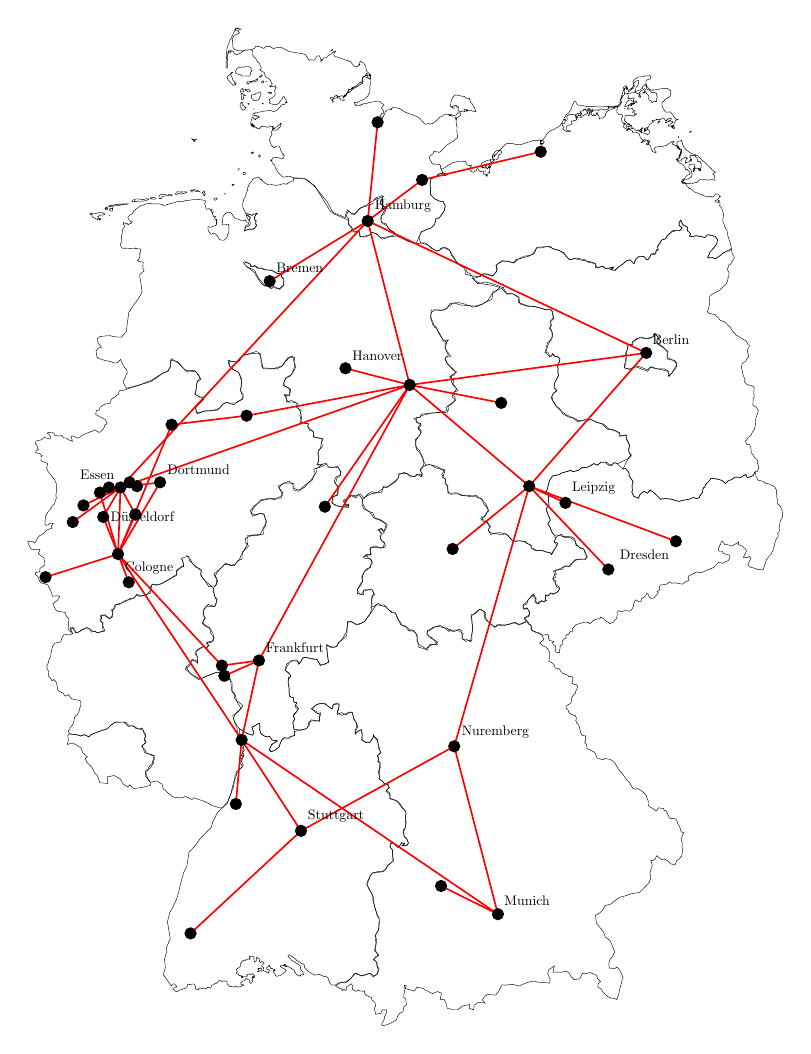
\begin{tikzpicture}

\definecolor{darkgray176}{RGB}{176,176,176}

\begin{axis}[
hide x axis,
hide y axis,
tick align=outside,
tick pos=left,
x grid style={darkgray176},
xmin=5.41798591613775, xmax=15.4935913085937,
xtick style={color=black},
y grid style={darkgray176},
ymin=46.8806100845338, ymax=55.4458555221558,
ytick style={color=black},
width=\linewidth,
height=1.28\linewidth
]
\addplot [line width=0.16pt, black]
table {%
8.70837306976324 47.7155570983886
8.71268272399902 47.7060623168946
8.71873188018799 47.6989135742188
8.71139812469477 47.6942787170411
8.69994831085216 47.6980361938477
8.69212532043457 47.6993370056152
8.68490028381348 47.6944847106934
8.67888832092291 47.6914443969727
8.66709423065197 47.6902580261231
8.66470623016357 47.6931343078614
8.66127586364757 47.6956634521484
8.66714191436779 47.6972236633302
8.67325878143305 47.6996383666992
8.67633533477795 47.705909729004
8.67048358917236 47.7113990783691
8.66622734069836 47.7148742675782
8.67177963256836 47.7169189453126
8.68023490905762 47.7178802490236
8.68641281127941 47.7136421203613
8.69133853912354 47.7165451049806
8.7006978988648 47.720142364502
8.70837306976324 47.7155570983886
};
\addplot [line width=0.16pt, black]
table {%
9.65046024322515 49.7763404846192
9.64671993255615 49.7352600097657
9.63594913482672 49.723991394043
9.63150024414062 49.6978416442872
9.68196868896479 49.7130584716797
9.734221458435 49.6947593688966
9.79042911529547 49.7175102233886
9.81357955932623 49.7102394104005
9.83292961120611 49.6546211242676
9.86216926574713 49.6362915039064
9.863450050354 49.6029090881348
9.84764003753668 49.5694007873536
9.84862041473389 49.5434799194336
9.88179874420172 49.5697097778321
9.92138957977306 49.5774688720703
9.93358993530279 49.5553703308107
9.9292192459107 49.5183410644531
9.92999839782721 49.4961585998536
9.98171043396007 49.4818916320802
10.0272397994996 49.4823112487794
10.0602989196777 49.5158119201661
10.0708284378052 49.5417518615723
10.0829687118531 49.5196914672852
10.1178789138795 49.4978485107423
10.1304388046265 49.4611091613771
10.1426296234131 49.4354286193848
10.1551504135133 49.3987312316896
10.1159391403199 49.3762817382813
10.1338491439819 49.3470115661622
10.1229391098022 49.3285102844239
10.1516275405884 49.3214416503906
10.1525583267212 49.2846908569336
10.1360483169556 49.2588005065918
10.1419305801392 49.2515106201172
10.1484308242798 49.2148399353028
10.1430997848511 49.1964187622071
10.1835393905641 49.1748085021974
10.2068395614625 49.1530303955078
10.2411603927612 49.1533889770509
10.2531890869142 49.1241607666016
10.2192888259888 49.0981292724609
10.2597303390504 49.0802116394044
10.2715091705323 49.0620002746582
10.271809577942 49.0436820983887
10.3179388046265 49.0331687927246
10.3584299087525 49.0189399719239
10.3934898376466 48.9899787902833
10.4167490005493 48.9682197570801
10.4391298294067 48.9606819152832
10.4558286666871 48.9457702636719
10.4669189453125 48.9272117614747
10.4555187225343 48.8977584838868
10.4665498733522 48.8644218444825
10.4607086181642 48.8238410949708
10.4493999481202 48.8091697692872
10.4437198638917 48.7981414794922
10.4323701858521 48.7760810852051
10.4378900527954 48.7575607299805
10.4490718841552 48.7426719665527
10.4770889282227 48.7239418029786
10.4938383102417 48.6941986083985
10.4712591171265 48.672248840332
10.4318799972534 48.6726303100586
10.4488496780395 48.6946296691895
10.4094686508179 48.6950187683105
10.3698692321777 48.6584815979004
10.3020696640015 48.6958007812501
10.2734708786012 48.6883697509767
10.2792100906373 48.6590385437012
10.301968574524 48.6369400024414
10.3018493652345 48.5963897705079
10.3073301315308 48.555690765381
10.2505998611451 48.5231018066407
10.2335996627809 48.5157890319825
10.2225599288942 48.4969596862794
10.1835803985596 48.4701118469238
10.1218395233155 48.4724998474122
10.0602903366089 48.4601097106934
10.0324802398682 48.4410095214843
9.99945068359381 48.3995895385743
9.98865890502935 48.3734092712402
10.011589050293 48.3403892517091
10.0457096099855 48.303810119629
10.0685291290284 48.2706718444825
10.0689191818237 48.2408599853516
10.0919904708862 48.1777496337892
10.1203107833863 48.1295204162598
10.1427507400513 48.1035804748536
10.1429491043091 48.0811614990234
10.1324081420899 48.0175285339355
10.0884895324708 47.9722709655763
10.110899925232 47.9388694763185
10.1001195907593 47.9014015197754
10.0948390960694 47.8639602661133
10.0949506759645 47.8452796936035
10.1060085296631 47.8416404724121
10.1281871795655 47.8156509399414
10.0951404571534 47.8078689575196
10.0731897354125 47.7852210998535
10.111780166626 47.7630691528321
10.1173086166382 47.7368392944336
10.1394691467285 47.7070999145508
10.1118392944337 47.6692314147949
10.0785303115844 47.6573905944824
10.0730514526367 47.6611213684083
10.0240898132324 47.6799316406251
9.97525978088385 47.6687393188477
9.92632865905762 47.6574096679688
9.84401988983154 47.6790313720703
9.81698989868164 47.6564903259277
9.78452968597423 47.6338920593263
9.74108982086193 47.6147994995117
9.70850086212164 47.6031799316406
9.67553997039806 47.6100387573242
9.64301013946533 47.5943489074708
9.61582946777344 47.5823020935059
9.60809707641602 47.5875549316407
9.59931564331055 47.5886344909669
9.59156322479254 47.5874824523926
9.58055114746094 47.5858955383301
9.56746578216564 47.5864715576173
9.55880260467541 47.5887489318848
9.55422782897955 47.591781616211
9.54609680175787 47.5974426269531
9.53862190246582 47.6039581298829
9.53589153289806 47.6126098632814
9.53309917449951 47.6181373596191
9.52856636047369 47.6193656921388
9.52529335021973 47.6254386901856
9.52381896972668 47.629135131836
9.52054023742676 47.6396560668946
9.51149272918713 47.6456222534181
9.50139141082775 47.6514587402344
9.48963165283209 47.6528053283691
9.48559665679932 47.6519966125489
9.4783754348756 47.6528930664062
9.47086143493658 47.651683807373
9.46423339843756 47.6545143127441
9.45750808715826 47.6581802368165
9.44812011718761 47.659523010254
9.43903255462652 47.6610946655273
9.42863941192627 47.6671295166016
9.42107486724848 47.6689834594727
9.4103507995606 47.6703491210938
9.39669227600092 47.6690368652344
9.39076995849609 47.6675834655762
9.3746967315675 47.6669807434082
9.36424160003662 47.6638488769532
9.35340976715088 47.664867401123
9.34339332580572 47.668212890625
9.33466625213634 47.6726226806641
9.32297325134272 47.6757583618165
9.31399726867681 47.6776199340821
9.30723381042486 47.6811218261718
9.29708385467535 47.6851539611817
9.29158020019531 47.689064025879
9.28154468536371 47.6937446594239
9.26723480224615 47.6994667053223
9.25749015808117 47.7048988342285
9.25014114379888 47.7104835510254
9.24290466308588 47.7170372009278
9.23632717132574 47.7226371765137
9.23141384124767 47.7293014526368
9.23014163970942 47.7369461059571
9.23065662384033 47.7432098388672
9.22443294525146 47.7482109069824
9.2136049270631 47.7519302368164
9.20805168151861 47.7532234191895
9.20123672485346 47.7544631958008
9.19145011901861 47.7590599060059
9.18303108215343 47.7624626159669
9.17338562011724 47.7661933898926
9.16315460205089 47.7707443237306
9.15264892578136 47.7739028930665
9.14535617828375 47.7753715515137
9.13589954376221 47.7795181274415
9.13059806823736 47.7854080200196
9.12322807312023 47.7908782958985
9.11534500122082 47.7942619323731
9.10388755798346 47.8007392883301
9.09918880462652 47.8025970458986
9.09108543395996 47.8041038513184
9.08247089385986 47.8089294433594
9.0749311447143 47.8122177124023
9.07011222839355 47.8168601989746
9.05317878723139 47.8216400146486
9.0467987060548 47.8235092163087
9.04012203216547 47.8222045898438
9.03320407867437 47.8167381286622
9.03183364868175 47.8129463195801
9.03997707366943 47.8063850402832
9.04921340942377 47.8014678955079
9.05444812774658 47.7963714599609
9.06152534484875 47.7916717529297
9.06891536712658 47.7852935791016
9.07866191864019 47.779483795166
9.08832454681402 47.7744712829591
9.09452724456787 47.7718505859376
9.1033754348756 47.7694129943848
9.11176872253429 47.7672576904297
9.12090778350841 47.7643127441406
9.12673091888422 47.7603073120117
9.13243103027355 47.7562713623046
9.13851070404064 47.7539863586426
9.15197944641108 47.7531929016113
9.15660190582281 47.7489128112794
9.1696834564209 47.7415885925294
9.17700290679932 47.7377548217775
9.17987060546881 47.7334213256836
9.18145370483398 47.7278709411622
9.18323516845703 47.723014831543
9.18505859375011 47.7189559936523
9.18371582031256 47.7103919982911
9.18822574615479 47.7066345214845
9.19218921661383 47.7022895812989
9.20068073272699 47.6975593566895
9.21247482299799 47.6903038024903
9.21541595458996 47.6844253540039
9.21637821197521 47.6759376525879
9.2215576171875 47.6689567565919
9.21742343902588 47.6667251586915
9.21097278594965 47.6650924682618
9.20100402832031 47.6685295104981
9.18757057189947 47.6692504882814
9.18506145477295 47.6643333435059
9.18147659301763 47.6574096679688
9.17087745666504 47.6605148315431
9.16667747497564 47.6618881225586
9.16502189636242 47.6571922302246
9.15844345092779 47.6579513549805
9.15294647216797 47.6605720520021
9.14853286743175 47.6659393310547
9.13695621490484 47.6681976318359
9.13035774230963 47.672836303711
9.12495899200434 47.6801300048829
9.11803817749035 47.6869888305665
9.11036586761475 47.688461303711
9.10772037506104 47.6919555664064
9.11163139343256 47.6946105957032
9.10950660705566 47.6994132995606
9.10383987426763 47.7048873901368
9.09731960296642 47.7083930969239
9.08959770202642 47.7112808227539
9.08130836486822 47.7134933471681
9.07031917572021 47.7178497314454
9.06135559082031 47.7216835021973
9.05045032501221 47.7261543273926
9.04244804382324 47.7277336120607
9.03370380401617 47.7314605712892
9.02359199523937 47.7336387634278
9.0131950378418 47.7391738891602
9.00182247161865 47.7456588745117
8.99239635467529 47.7479782104493
8.98550701141357 47.7454147338867
8.98817157745373 47.7411727905275
8.99635124206549 47.738452911377
9.0031938552857 47.7357177734375
9.01009559631348 47.731315612793
8.99729061126715 47.7321701049805
8.98511028289789 47.7368774414062
8.97660160064703 47.7398071289063
8.96861362457287 47.7408981323243
8.95772552490246 47.7418823242188
8.95046997070324 47.7406311035156
8.94417381286615 47.7381248474121
8.94136524200445 47.7318229675293
8.94789314270014 47.7273674011232
8.95422363281256 47.7254943847657
8.96321487426758 47.7214126586914
8.97292327880865 47.7169494628907
8.97875118255615 47.7149810791016
8.98491859436035 47.7132148742677
8.99152565002453 47.7115745544434
8.99672508239752 47.7102661132814
9.00337696075445 47.7057037353517
9.00872898101807 47.7000312805176
9.00550270080566 47.6943664550782
8.99800872802729 47.6882476806641
8.99105644226086 47.6840248107911
8.98582363128662 47.6820831298828
8.9809455871582 47.6804008483888
8.9737167358399 47.6746253967286
8.96322441101086 47.6727447509766
8.95596313476568 47.6699180603028
8.94959831237799 47.6669654846191
8.94071388244635 47.661678314209
8.92500972747808 47.6613731384278
8.91370391845697 47.6579627990723
8.90520191192638 47.6567687988281
8.89183425903332 47.6552238464357
8.87854003906256 47.6658515930176
8.87299537658691 47.6762657165527
8.86657619476318 47.6817436218263
8.860016822815 47.6839294433595
8.8548383712768 47.6879997253419
8.85904026031494 47.6944732666015
8.85572910308832 47.6989555358886
8.85916233062738 47.7020797729493
8.86531639099127 47.7003784179689
8.86726093292248 47.6974258422852
8.87013912200939 47.6968231201172
8.87787246704107 47.6989212036133
8.87658691406256 47.7021064758301
8.87370681762707 47.7049293518066
8.87209320068371 47.7085342407228
8.8550767898559 47.7081947326661
8.84860324859625 47.7121810913087
8.84465408325201 47.7162895202638
8.83664035797131 47.7179412841796
8.82831192016613 47.7151031494141
8.82244777679455 47.7168884277344
8.82460021972668 47.7212753295899
8.82076835632319 47.7217826843262
8.81555271148682 47.7270812988282
8.80809402465832 47.7294616699219
8.81241321563721 47.7334556579591
8.81119728088379 47.7357864379883
8.80929374694836 47.740249633789
8.80632114410412 47.7417984008789
8.79995632171642 47.7387847900391
8.79578304290783 47.7325515747071
8.78918266296392 47.7320938110352
8.78331184387207 47.7271347045898
8.77269458770752 47.7218818664551
8.77110385894775 47.7186965942382
8.77216911315918 47.7119445800782
8.78043079376226 47.7097396850585
8.79748630523687 47.7072372436525
8.79992485046398 47.7030181884767
8.80505752563488 47.7002639770508
8.80853271484381 47.6978797912598
8.80264472961431 47.69637298584
8.79735946655279 47.6904220581056
8.79629611968994 47.6814765930176
8.79178714752209 47.6793975830079
8.78179740905773 47.6826667785645
8.77375507354742 47.6864814758301
8.76686096191406 47.6908988952638
8.75304985046381 47.6949806213379
8.73966598510742 47.6966819763184
8.72960376739502 47.7051963806153
8.73334026336664 47.7132644653321
8.73743343353266 47.7203712463379
8.73475837707525 47.7235221862794
8.72563266754162 47.7267379760742
8.71699523925793 47.7299385070801
8.7134313583374 47.7350196838379
8.71482753753668 47.7417640686036
8.71932792663574 47.7455215454102
8.72465801239019 47.7497825622559
8.73334789276123 47.7511138916017
8.74229717254633 47.7527999877931
8.74053764343267 47.7580528259278
8.73138332366943 47.7633056640626
8.72906875610357 47.7671165466309
8.71936130523676 47.7701454162598
8.71004867553722 47.7696342468262
8.70104694366461 47.7657661437988
8.69786643981939 47.7621459960939
8.69301700592052 47.7624855041504
8.68807888031006 47.7706794738769
8.68549633026123 47.7755165100098
8.68839740753174 47.7802963256837
8.68372154235846 47.7855491638183
8.68181514739996 47.7921981811523
8.67188072204596 47.793399810791
8.66308689117426 47.7966003417969
8.66181182861334 47.8009719848633
8.65870666503906 47.8051910400391
8.65114688873291 47.8051300048828
8.64780712127691 47.7999229431152
8.64606094360352 47.7959175109863
8.64925193786632 47.7908935546876
8.64937305450445 47.7808074951172
8.64617824554449 47.7741088867188
8.64328956603998 47.771224975586
8.64021873474127 47.7699737548829
8.63050937652588 47.7657737731934
8.62617301940929 47.7697601318361
8.62173557281494 47.7739295959473
8.62348842620855 47.7819099426271
8.62011241912847 47.7851753234863
8.61669158935558 47.7901153564454
8.61961269378662 47.7944793701172
8.62158775329601 47.8017196655273
8.61474895477295 47.8076362609864
8.60294437408453 47.8091011047364
8.59474372863775 47.8063049316406
8.59028244018566 47.8076667785646
8.58341407775879 47.8077354431152
8.57697010040278 47.8070449829102
8.57386779785156 47.8120498657227
8.5686759948731 47.8143997192384
8.56313991546631 47.8113059997558
8.56232833862305 47.7999725341797
8.56805992126465 47.7970008850097
8.57480812072748 47.7928314208985
8.57164669036877 47.7875518798828
8.56379985809326 47.7875175476074
8.55491924285894 47.7910957336426
8.5483484268189 47.7901306152344
8.53843688964849 47.7880249023438
8.52550315856928 47.7843322753906
8.52108097076422 47.778305053711
8.51064491271978 47.7829437255861
8.50574398040771 47.7810249328613
8.49781322479248 47.7789306640626
8.49124526977545 47.7793998718263
8.48542690277111 47.778175354004
8.47800254821772 47.7733230590821
8.47058391571051 47.7679901123047
8.46823215484619 47.7631912231445
8.46524238586431 47.759693145752
8.45897006988537 47.757610321045
8.45654582977306 47.7513618469239
8.45364570617687 47.7474555969238
8.45261192321789 47.7400283813478
8.45591640472406 47.7332649230958
8.44421100616466 47.727840423584
8.44092559814453 47.7240943908693
8.43522071838379 47.723545074463
8.42614078521734 47.718246459961
8.41727733612055 47.7165603637696
8.4077291488648 47.7081985473634
8.40561485290533 47.7034225463868
8.41038513183594 47.7012672424316
8.41483974456793 47.6950988769531
8.41806221008301 47.690773010254
8.41506671905518 47.6867370605469
8.40631771087641 47.6838836669922
8.40472316741949 47.6787452697753
8.41301155090343 47.6720390319825
8.42396926879894 47.6713371276855
8.43025398254395 47.6682739257813
8.43540000915533 47.6643829345703
8.44223690032959 47.6607704162599
8.45190620422369 47.6595458984376
8.46172237396246 47.6596946716309
8.46718406677246 47.6611022949218
8.4658727645874 47.6533050537109
8.46818065643322 47.6453437805177
8.47563457489025 47.6434135437013
8.47862529754644 47.6453018188477
8.47322654724132 47.6467018127441
8.47423934936529 47.6486663818361
8.47744941711431 47.6503562927246
8.47510719299316 47.6544380187989
8.48215579986572 47.6535263061523
8.48421001434338 47.6495628356933
8.48891162872314 47.6482238769532
8.49495410919184 47.6478042602539
8.49670696258551 47.6515541076661
8.50172328948975 47.6520919799806
8.52180194854748 47.6509819030762
8.53375244140619 47.651035308838
8.53589725494385 47.6544456481934
8.5318603515625 47.6618843078614
8.5327262878418 47.6667861938478
8.53828525543219 47.663917541504
8.54125499725336 47.6647453308106
8.54394912719721 47.6703720092774
8.56136226654064 47.674674987793
8.57065582275396 47.6691246032715
8.57901000976562 47.6675910949708
8.58792495727545 47.6708793640138
8.59741973876964 47.6745796203613
8.60257434844971 47.6769714355469
8.61126804351807 47.6683006286621
8.61979579925537 47.6639213562012
8.62553977966314 47.6598205566406
8.6293888092041 47.6535186767578
8.6250953674317 47.6458625793458
8.61572360992437 47.6416931152344
8.60432529449474 47.64315032959
8.60906410217291 47.6462898254396
8.61533355712902 47.6501846313478
8.61017990112305 47.6560173034669
8.60499000549316 47.6551628112794
8.59684658050548 47.6471939086914
8.59804725646984 47.6345481872559
8.60279464721685 47.6254615783692
8.60586929321295 47.6168937683107
8.59806728363037 47.6113128662109
8.59033775329601 47.6057624816895
8.58634185791027 47.6028289794922
8.58178424835205 47.5997772216797
8.57199287414551 47.6011924743653
8.56536293029791 47.609031677246
8.5719194412232 47.6148300170899
8.57200813293457 47.6178207397461
8.56497573852539 47.6212997436523
8.55906963348389 47.6276054382325
8.54800891876221 47.6295013427734
8.54068088531494 47.631519317627
8.53899097442638 47.6347961425781
8.53183078765881 47.636344909668
8.52302646636969 47.6379623413087
8.51887035369879 47.6365852355956
8.51397514343267 47.6293640136719
8.50899219512945 47.6270828247071
8.50658226013195 47.6221199035645
8.49603366851807 47.6191177368165
8.48259353637695 47.618637084961
8.47723865509033 47.6142082214356
8.47123908996576 47.6092948913575
8.46470355987549 47.6075019836426
8.45824337005615 47.6053199768066
8.45950031280518 47.6011848449708
8.46142673492437 47.5941162109376
8.46748924255382 47.5896759033204
8.47150897979731 47.5885543823243
8.48195743560791 47.5894660949708
8.49204444885254 47.5909423828125
8.48968315124512 47.582763671875
8.47814178466803 47.581356048584
8.47262668609625 47.5788688659669
8.45789909362799 47.5765266418457
8.44715595245361 47.5738372802735
8.43453121185314 47.5713272094727
8.42343139648443 47.5707511901857
8.41617393493664 47.5744094848633
8.40685558319092 47.577709197998
8.39744186401379 47.580150604248
8.38742160797125 47.5745353698731
8.38315677642822 47.5703124999999
8.37329864501964 47.5716209411622
8.35743618011486 47.5742416381837
8.33047389984131 47.5747642517091
8.32132053375244 47.5784606933595
8.31454944610596 47.5834808349609
8.29977798461925 47.5913276672364
8.29470157623297 47.5965003967286
8.29558563232422 47.6082000732422
8.29330921173107 47.6126823425294
8.28142738342297 47.6163368225099
8.27288818359375 47.6161689758302
8.26095867156988 47.6178894042969
8.25420379638672 47.620059967041
8.24035167694092 47.6181640625001
8.23482704162603 47.6162605285645
8.22952365875256 47.6115531921388
8.22291278839117 47.6130638122559
8.21815490722656 47.622573852539
8.2067956924439 47.6262550354005
8.19632816314709 47.6241264343262
8.18986892700201 47.6179962158203
8.18776798248302 47.6148719787598
8.18297386169434 47.6098442077638
8.1759462356568 47.6084938049318
8.17027664184582 47.6041145324708
8.16212463378912 47.5996131896973
8.15146446228022 47.6012763977052
8.14140129089355 47.5982208251953
8.13720417022705 47.5918617248536
8.13370609283453 47.5890541076661
8.11497402191168 47.5892066955567
8.10432720184326 47.5844078063965
8.10028171539307 47.5709686279297
8.09580707550049 47.5655212402345
8.08651161193859 47.5628051757813
8.07672309875494 47.5660247802735
8.0710134506225 47.5700035095216
8.06526947021496 47.569881439209
8.05796813964849 47.5688858032227
8.04987525939953 47.5635643005371
8.03913402557379 47.5593109130859
8.01532363891607 47.5568771362305
8.00687599182135 47.5593643188477
7.9995379447937 47.5624160766602
7.98657608032238 47.5614891052246
7.97047805786133 47.5616455078126
7.9571299552918 47.56400680542
7.95049285888666 47.5555419921876
7.94698715209961 47.5500297546387
7.93535804748541 47.5523071289063
7.91738605499279 47.5539131164551
7.90874481201172 47.5603256225587
7.90722417831415 47.5685386657715
7.91026782989508 47.5759582519532
7.90484380722052 47.5839538574219
7.89448404312134 47.5920257568361
7.88652515411371 47.5948944091798
7.86763381958008 47.5952033996581
7.85302877426147 47.5913429260255
7.84006214141851 47.5888862609864
7.83285522460938 47.5925521850587
7.82077217102056 47.5946998596192
7.81562089920044 47.5909194946289
7.8118138313294 47.5827026367187
7.80856800079346 47.5754699707031
7.80025911331177 47.5706901550294
7.79436206817638 47.5646133422852
7.78735065460205 47.5618591308595
7.77046012878424 47.5591278076172
7.75716018676769 47.5557289123535
7.75042819976801 47.5516777038575
7.72458600997925 47.5497512817383
7.70842981338501 47.5442657470704
7.69653606414795 47.5389595031738
7.68693876266479 47.5361022949219
7.66517782211309 47.538833618164
7.6569390296936 47.5460662841798
7.65017890930176 47.5495491027833
7.64268398284912 47.5519828796387
7.63682699203503 47.5587043762208
7.63945198059076 47.5631065368653
7.64800930023193 47.56498336792
7.66280603408825 47.5679054260255
7.6720399856568 47.5717277526857
7.67832088470459 47.5705413818359
7.68170309066772 47.5735359191895
7.67740488052362 47.5763473510743
7.67208814620966 47.5850105285645
7.66676616668701 47.5863838195802
7.6645069122315 47.5893058776855
7.65889120101934 47.5940628051758
7.64944601058954 47.5961647033691
7.63876819610596 47.5969467163087
7.63531112670898 47.5926742553711
7.62842178344721 47.5879516601563
7.62015104293823 47.5820465087891
7.60277509689337 47.5896835327149
7.57183313369745 47.6214981079102
7.52001142501837 47.6680755615235
7.5438866615296 47.7225837707521
7.53389596939093 47.7902183532715
7.56260490417486 47.853084564209
7.55832004547131 47.8812789916993
7.60334253311157 47.9485626220703
7.56931543350231 48.0806770324707
7.58777141571039 48.1280059814454
7.59949970245361 48.1556320190431
7.63713073730469 48.195873260498
7.68145990371715 48.2596397399903
7.70507860183727 48.3096351623536
7.73096609115606 48.3822059631348
7.76616191864014 48.4639739990235
7.80516195297247 48.5135002136231
7.83175373077404 48.6232795715332
7.8962516784668 48.6672096252442
7.96770238876343 48.7297859191895
8.01622200012213 48.7623977661132
8.05623722076416 48.7896461486816
8.10069656372065 48.8154487609864
8.11810111999506 48.8563079833984
8.16850566864019 48.9245033264161
8.23029518127453 48.9672966003419
8.2952995300293 49.0041503906251
8.3408002853393 49.0840110778809
8.36952018737793 49.1632385253907
8.40528869628912 49.2203521728515
8.40367889404291 49.2499122619629
8.48058891296392 49.289821624756
8.45673084259039 49.3183708190919
8.49954032897961 49.3787803649902
8.46553993225098 49.3775291442872
8.50355815887451 49.4229621887208
8.44516944885254 49.4612503051757
8.44361877441412 49.501579284668
8.44622039794922 49.5861892700195
8.5276603698731 49.5521697998047
8.60262966156006 49.5363311767579
8.61937904357916 49.5515289306641
8.59504890441895 49.5983886718749
8.68616867065435 49.6305313110352
8.69249820709229 49.6087417602539
8.68750858306879 49.5793113708497
8.70555973052984 49.5469322204591
8.74616146087658 49.529811859131
8.78079032897955 49.5234107971192
8.80945873260498 49.527759552002
8.83880996704113 49.4992408752442
8.90242958068853 49.4930992126465
8.86804866790783 49.4779396057128
8.83375930786138 49.4626922607422
8.80581855773926 49.4220085144044
8.82904815673828 49.4079818725587
8.87488937377924 49.4197616577149
8.92646980285656 49.4459686279298
8.93756866455078 49.4716491699219
8.95446014404308 49.4974212646485
8.9830493927002 49.5160217285156
9.04674911499023 49.5128517150878
9.06380844116217 49.527629852295
9.1041898727417 49.5314521789551
9.11559867858898 49.5388298034668
9.10931968688976 49.5645904541017
9.18978977203375 49.5793418884278
9.25874996185303 49.5864486694337
9.27552032470697 49.6085815429688
9.28634071350103 49.6381416320802
9.31462955474865 49.6565589904786
9.41805934906012 49.6452293395996
9.41161823272716 49.6711921691895
9.4280300140382 49.6971321105957
9.39357852935802 49.7045593261719
9.35892868042004 49.7193984985352
9.34142971038824 49.7342185974122
9.31266880035406 49.7416610717773
9.36345958709722 49.767520904541
9.43115901947021 49.7861289978028
9.48233985900879 49.77885055542
9.51671981811523 49.7641105651855
9.56256961822521 49.7420196533203
9.58343982696545 49.7794418334961
9.65565872192388 49.7875595092775
};
\addplot [line width=0.16pt, black]
table {%
10.1338596343995 50.5499992370606
10.175030708313 50.5463218688965
10.2220582962036 50.5388488769532
10.25749874115 50.5127105712891
10.3105001449586 50.4940490722657
10.3458290100097 50.4828720092773
10.3696393966674 50.4418487548828
10.3815002441407 50.4269409179687
10.3933992385864 50.4082794189453
10.4287796020508 50.3896713256837
10.4935398101807 50.3711090087891
10.5171899795533 50.3487510681153
10.5583114624024 50.3525505065919
10.5996913909913 50.3190307617188
10.5999088287354 50.2853622436525
10.605890274048 50.2666816711426
10.6177797317505 50.2442588806153
10.6647691726684 50.2294197082521
10.7230186462403 50.1997985839844
10.7518301010132 50.2447204589844
10.8093795776368 50.241310119629
10.8495798110962 50.2638320922853
10.8035392761232 50.2822418212891
10.7690296173095 50.2932815551758
10.7172508239746 50.322940826416
10.7224493026733 50.3526611328126
10.7798700332641 50.3675994873048
10.8199300765991 50.3825187683106
10.8772802352905 50.3937797546387
10.9118385314942 50.3827590942383
10.9868106842042 50.3459205627443
10.9981107711791 50.3644790649415
11.0385084152223 50.3423614501954
11.1132392883301 50.3648986816407
11.1421594619752 50.3501586914063
11.1421003341676 50.3167495727539
11.1596403121949 50.2834587097168
11.1940393447877 50.2872505187988
11.2516689300537 50.2651901245118
11.2518787384034 50.2911415100098
11.2640590667726 50.3320198059083
11.2763004302979 50.3803787231446
11.2649793624878 50.4100494384766
11.2652893066406 50.4397888183594
11.2540006637574 50.4806289672852
11.3007707595826 50.480812072754
11.347978591919 50.5144386291504
11.3831501007081 50.514560699463
11.4180603027344 50.492359161377
11.4175081253052 50.4514503479003
11.4523401260377 50.4254989624024
11.4814081192017 50.4069709777833
11.5165004730225 50.395881652832
11.5514888763429 50.3810615539552
11.5987586975097 50.3997993469238
11.6690998077392 50.3962516784669
11.7279195785524 50.4038391113282
11.763279914856 50.4113807678224
11.781060218811 50.4188995361329
11.8332996368409 50.4041213989258
11.8683385848998 50.4042091369629
11.9332876205445 50.4230957031251
11.9508810043336 50.4051361083985
11.9728994369507 50.40087890625
11.988410949707 50.3786888122559
11.980833053589 50.3621330261232
11.9984741210938 50.3524780273438
12.042724609375 50.337890625
12.0652704238892 50.3379096984864
12.0980758666992 50.3269500732423
12.1192445755005 50.3130340576173
12.1273336410524 50.2997283935546
12.1371698379517 50.2821121215821
12.0858602523804 50.2553520202638
12.1089019775391 50.2439460754395
12.1319217681885 50.2320747375489
12.161280632019 50.2252082824708
12.1852025985718 50.2088623046876
12.1989192962646 50.1956214904786
12.2102556228639 50.171459197998
12.1990604400635 50.1118202209473
12.2236337661744 50.1068382263184
12.2387990951538 50.1005210876465
12.2619924545289 50.087646484375
12.2671489715576 50.074031829834
12.2734403610229 50.0612945556642
12.3019199371339 50.058864593506
12.3234615325928 50.0559158325196
12.3403053283693 50.0390205383301
12.3644390106201 50.0203819274903
12.3873596191406 50.0163803100587
12.4103908538818 50.0084609985353
12.4300937652589 50.0047760009766
12.4392223358154 49.9918441772462
12.4683113098146 49.9958801269531
12.4915103912355 49.9839515686036
12.4858713150024 49.9634895324708
12.474949836731 49.9445724487304
12.4975881576538 49.9344406127931
12.5331840515136 49.930633544922
12.5491809844971 49.9181823730469
12.5444335937501 49.9042472839355
12.526593208313 49.8848419189454
12.5192785263063 49.8639907836915
12.5033111572267 49.8559761047363
12.4783086776733 49.8320312500001
12.4698915481567 49.8037109375001
12.4658308029174 49.7857551574708
12.4473314285279 49.779411315918
12.4087495803834 49.7661895751954
12.4084739685059 49.7448501586915
12.4312286376953 49.7328186035157
12.4406900405884 49.7154693603517
12.4583139419557 49.7031402587891
12.4862108230591 49.6961135864258
12.4951152801514 49.6907997131347
12.516598701477 49.6916007995605
12.5329446792603 49.6718978881837
12.5283613204957 49.6570854187012
12.5227203369141 49.6488914489746
12.5303115844727 49.6449050903321
12.536660194397 49.6285514831544
12.5528450012207 49.6246528625488
12.55885887146 49.6174087524415
12.5703268051148 49.5979232788087
12.5753774642945 49.5801544189454
12.5844507217407 49.5536079406739
12.5942611694337 49.5408020019531
12.6154766082764 49.5331649780273
12.6458301544191 49.5310592651367
12.6443939208985 49.4944534301758
12.6328067779542 49.4800148010255
12.6467456817628 49.471939086914
12.6570024490356 49.4582099914551
12.6610746383668 49.4321670532227
12.6898450851441 49.4251441955566
12.7193031311036 49.4136276245117
12.7555837631226 49.4025840759278
12.7829885482788 49.3591842651368
12.8576192855836 49.3436088562013
12.8767499923707 49.3545112609864
12.9411487579346 49.3486595153809
12.9804162979126 49.3320274353027
13.0011110305786 49.3171577453613
13.0326108932496 49.282730102539
13.0609884262086 49.2558517456055
13.0954179763795 49.2338256835938
13.0999822616577 49.2223091125489
13.1145906448364 49.2165374755859
13.1311626434327 49.1972122192383
13.1542034149171 49.1806259155275
13.1691198349 49.1725578308107
13.1861791610718 49.1554489135743
13.2177381515503 49.1211318969728
13.2482128143311 49.1143608093263
13.2749977111816 49.1206436157227
13.3338308334351 49.0973205566407
13.3769292831421 49.0707321166993
13.4074516296388 49.0151824951172
13.4071636199951 48.9933280944824
13.4084062576295 48.9843482971191
13.4374084472656 48.9726219177247
13.4663915634155 48.9608879089355
13.4885816574097 48.9487113952637
13.5033550262451 48.9451217651367
13.5268354415895 48.9692535400391
13.5613679885865 48.9668998718262
13.5891103744508 48.9641113281251
13.5981464385987 48.9477691650392
13.6144990921021 48.9491691589357
13.6252593994141 48.9433708190918
13.634614944458 48.9307212829589
13.6433172225952 48.9167137145997
13.6576251983643 48.8959197998046
13.6675214767456 48.8887939453126
13.697340965271 48.8847885131837
13.72260761261 48.8853912353517
13.736798286438 48.8813133239747
13.7519311904907 48.8700218200685
13.7616329193116 48.847972869873
13.7695722579957 48.8394012451173
13.7775077819825 48.8308258056642
13.7888803482057 48.8169898986818
13.804204940796 48.7826385498047
13.8359575271606 48.7750511169435
13.8235597610474 48.7606811523437
13.8042993545533 48.7282905578614
13.8144683837891 48.7027778625489
13.8162641525269 48.660327911377
13.8200798034668 48.6297721862793
13.8099441528321 48.59090423584
13.7608966827392 48.5613784790039
13.7489957809449 48.5570755004883
13.7286520004272 48.522789001465
13.6723461151123 48.5339279174805
13.6453313827515 48.5543746948242
13.6019525527955 48.5706596374512
13.5657234191895 48.5662689208986
13.5085992813111 48.5963897705079
13.4908790588379 48.5746192932128
13.466835975647 48.5603561401368
13.435447692871 48.5598144531251
13.4545402526856 48.516300201416
13.4411983489991 48.4977531433105
13.4236793518068 48.4577789306642
13.437659263611 48.4363365173339
13.4201545715332 48.3915367126465
13.3686418533325 48.3558235168458
13.297986984253 48.3099098205566
13.1977338790894 48.2989654541016
13.1412687301636 48.2855300903321
13.058403968811 48.2717361450196
13.0034379959107 48.2465362548829
12.9463319778442 48.21732711792
12.8824644088746 48.2075424194337
12.8559894561769 48.1768112182618
12.8324937820435 48.1590919494629
12.7974910736085 48.1415252685548
12.7647256851196 48.1320304870606
12.7737283706666 48.0727195739747
12.8640136718749 47.9982185363769
12.8832569122315 47.960521697998
12.91832447052 47.9440841674805
12.942084312439 47.9312858581543
12.9666528701782 47.8963623046876
12.9973659515381 47.8474273681642
12.971534729004 47.809497833252
12.9376850128173 47.7854537963867
12.9261684417725 47.7532806396484
12.9307203292847 47.7189598083497
12.9976987838746 47.7162590026857
13.023491859436 47.7256660461425
13.05153465271 47.7115440368652
13.0790977478027 47.6757202148438
13.0995168685914 47.6454505920411
13.0879936218263 47.6294746398927
13.076530456543 47.5950012207032
13.0589895248414 47.5579109191895
13.048776626587 47.5206642150879
13.0242395401 47.4727592468262
12.9931430816652 47.4817504882814
12.9473209381104 47.4861221313477
12.9130592346192 47.4967422485352
12.857219696045 47.5283584594727
12.8396644592286 47.5513954162598
12.7920913696288 47.572364807129
12.7970190048219 47.5989112854004
12.8250036239625 47.6143913269044
12.7875633239747 47.6385955810546
12.7791461944581 47.6621894836426
12.756314277649 47.670021057129
12.6943368911743 47.6846656799316
12.6443052291871 47.6741828918457
12.6053342819214 47.6792488098145
12.5741014480591 47.6348838806152
12.5056247711183 47.6290473937989
12.4667396545411 47.6541442871094
12.4402570724487 47.6813812255859
12.4086751937867 47.6962356567383
12.3621530532838 47.6880836486816
12.2970485687257 47.6876602172852
12.2479887008668 47.6875000000001
12.2648983001709 47.7364311218262
12.1988801956177 47.7064285278321
12.1838417053223 47.6771430969239
12.2121057510375 47.6326789855958
12.2092800140381 47.6012001037598
12.1544904708863 47.6053619384767
12.0608491897584 47.6101417541504
12.0168094635009 47.618049621582
11.9396581649781 47.6077308654786
11.8348293304444 47.5792884826661
11.7907781600952 47.5871620178224
11.7553968429565 47.5922279357911
11.6676912307739 47.5862731933595
11.6300992965699 47.5884780883789
11.608759880066 47.5632514953614
11.5926008224488 47.5417556762695
11.5534496307373 47.5084190368652
11.4484786987305 47.5131607055665
11.4125556945802 47.4922332763672
11.3905820846558 47.4707946777344
11.4240808486939 47.4456214904786
11.3416061401367 47.4518241882324
11.2938966751099 47.4301986694337
11.2849788665772 47.3948822021484
11.2355899810791 47.4031791687012
11.2359476089478 47.434196472168
11.1511888504028 47.4235649108887
11.0972509384155 47.3957214355469
11.0232343673707 47.3962020874023
10.9648666381835 47.4060363769532
10.9496288299561 47.4460220336915
10.9265918731689 47.4762153625488
10.8790102005005 47.4740905761719
10.8887186050416 47.5056991577148
10.8941373825074 47.5243263244629
10.845311164856 47.5358276367188
10.7874727249146 47.5203704833984
10.7612400054932 47.5273323059082
10.7269411087036 47.5400238037109
10.6975908279419 47.5456695556642
10.6754474639893 47.5601463317871
10.599970817566 47.5698318481446
10.5791826248169 47.5540237426758
10.5614671707154 47.5397911071778
10.453429222107 47.5610198974609
10.4698295593262 47.5809860229492
10.4459648132324 47.5856666564941
10.4517965316772 47.5575599670411
10.4396677017212 47.5170974731445
10.4384460449219 47.4881553649903
10.4626731872559 47.4797286987305
10.4648036956788 47.4579162597657
10.4700441360474 47.43265914917
10.4349317550659 47.4137001037598
10.4302892684937 47.3823738098145
10.3843297958375 47.3636360168458
10.3621091842652 47.3408699035645
10.3452501296998 47.3139190673829
10.2851896286011 47.2917213439943
10.2363986968995 47.2772216796876
10.1813392639161 47.2699394226075
10.1692867279053 47.2791099548341
10.1761407852174 47.2925491333009
10.2038888931274 47.3231086730958
10.2019653320312 47.3358116149902
10.2262201309204 47.3686408996582
10.2268695831299 47.3929176330567
10.178505897522 47.3934936523437
10.1606607437134 47.3672485351563
10.0961999893189 47.3585090637207
10.0808954238892 47.4045257568361
10.0949831008912 47.4233703613282
10.0886058807373 47.4506454467774
10.0553798675537 47.466869354248
10.0433826446534 47.4893760681152
9.99119472503662 47.5032081604005
9.96118831634516 47.5230407714844
9.96367740631115 47.5411643981935
9.94481468200684 47.5389022827148
9.90803241729742 47.54056930542
9.88100242614757 47.5485458374025
9.85710906982422 47.5382194519043
9.81310176849371 47.5524559020997
9.82004165649414 47.5752944946289
9.8015394210816 47.5971603393556
9.74723911285395 47.5741691589357
9.73667144775402 47.5472412109375
9.73229598999023 47.5453567504883
9.72355270385748 47.5503120422364
9.70933628082275 47.5516967773438
9.70098495483398 47.5486297607422
9.6951141357423 47.5439605712892
9.68802356719971 47.5443000793457
9.68502902984631 47.547721862793
9.68946456909191 47.5498428344728
9.69080257415777 47.5552864074708
9.68641662597656 47.5583343505859
9.67394638061529 47.5574188232422
9.66531181335461 47.5581893920899
9.65615940094 47.5600166320801
9.65301132202154 47.5647773742676
9.64020729064953 47.5679283142089
9.6367712020874 47.5708465576173
9.63286781311035 47.5715637207032
9.62277412414551 47.570915222168
9.61513328552257 47.5761795043946
9.61192798614502 47.5812339782716
9.62124824523926 47.5862388610839
9.63741016387951 47.6017799377442
9.67562007904064 47.6063308715821
9.71927928924561 47.6107521057129
9.74122905731201 47.6073989868165
9.7954092025758 47.637722015381
9.82240962982183 47.660270690918
9.86045074462902 47.6791992187501
9.93178081512451 47.657440185547
9.98069953918468 47.6687507629395
10.0295095443726 47.6761589050294
10.0674896240234 47.6497421264649
10.0895986557007 47.6650619506837
10.1118097305298 47.6729621887208
10.1283702850342 47.7069396972656
10.1117887496948 47.7367897033691
10.1062688827515 47.7667694091796
10.0676794052124 47.7851715087891
10.1006603240967 47.8041801452637
10.1336984634399 47.8194389343262
10.1059894561769 47.8453788757325
10.089409828186 47.8489799499512
10.083830833435 47.8601303100587
10.1000576019287 47.9088706970215
10.0942192077638 47.9499092102052
10.093999862671 47.9760589599609
10.132378578186 48.0212707519531
10.137399673462 48.0811004638671
10.1371698379517 48.1072616577148
10.1147499084473 48.1294593811035
10.0919103622437 48.1852188110353
10.0632390975952 48.2482414245607
10.0628490447998 48.2780303955079
10.0400190353395 48.311149597168
10.011480331421 48.3478202819825
9.98871994018566 48.3697013854981
10.0161504745483 48.4073295593263
10.0324296951295 48.4447288513183
10.0658416748047 48.4639205932617
10.1275291442872 48.4652099609376
10.1835393905641 48.4738197326661
10.2281589508057 48.4970588684082
10.2392406463624 48.5158500671388
10.2562789916992 48.5267295837403
10.3129796981812 48.5556297302247
10.3018903732301 48.6074600219727
10.3019781112672 48.6406211853027
10.2677593231202 48.6626586914062
10.2791976928711 48.6920700073242
10.3077697753906 48.6958007812501
10.3755283355712 48.662109375
10.4151096343995 48.6986618041993
10.4432096481324 48.690990447998
10.4149894714356 48.6728019714357
10.4825496673585 48.6795310974121
10.4938497543336 48.6978912353517
10.4715013504029 48.7313690185547
10.443440437317 48.7427101135254
10.4379081726075 48.7612495422364
10.4379787445069 48.7760314941407
10.4324893951417 48.7982521057129
10.4550285339356 48.8091201782228
10.4607696533203 48.8349189758302
10.4609394073487 48.8644714355469
10.4555492401122 48.9014587402344
10.4557399749755 48.9309997558595
10.4558382034302 48.9494590759277
10.4335298538209 48.9607200622559
10.4167718887329 48.975570678711
10.3932991027833 49.0009803771973
10.3641099929811 49.0226593017579
10.312189102173 49.0331115722656
10.2661209106446 49.0399513244629
10.2713899612427 49.0693397521974
10.2595386505128 49.0912094116212
10.2249002456665 49.1055221557618
10.2645597457885 49.1279411315917
10.241008758545 49.1607208251953
10.2067699432374 49.1567001342773
10.1777496337891 49.1784210205078
10.1374588012695 49.1926918029786
10.1427192687988 49.214771270752
10.1247301101685 49.2550086975098
10.1417598724366 49.2588500976564
10.1409692764282 49.2919197082521
10.1515302658082 49.3251190185547
10.1228504180908 49.3321914672852
10.1336507797241 49.3543701171876
10.1215295791627 49.3800086975098
10.1608381271362 49.398780822754
10.1312484741212 49.4353294372559
10.1246318817138 49.4647407531739
10.1235790252686 49.4979019165039
10.0885486602783 49.5234298706054
10.0710792541504 49.5343589782716
10.0660009384156 49.5158615112305
10.0216703414918 49.4785690307618
9.97614860534674 49.478141784668
9.92974090576166 49.5035514831543
9.93437862396246 49.5331802368164
9.92776012420654 49.5590209960938
9.92124938964849 49.5811805725098
9.87067890167248 49.5621910095216
9.84847831726074 49.5471801757813
9.85333061218267 49.569450378418
9.88053894042963 49.6030616760253
9.85631942749029 49.6399612426759
9.83248996734613 49.6657600402833
9.8134298324585 49.7139587402345
9.7847194671632 49.7174720764161
9.72245979309076 49.7021217346191
9.68297863006603 49.6907005310059
9.63645935058594 49.7127990722657
9.63018035888678 49.7276687622071
9.64653968811029 49.7389907836914
9.65614891052257 49.7763710021973
9.58359909057629 49.775718688965
9.57377910614014 49.742099761963
9.52826023101801 49.7567405700685
9.48785972595221 49.7825813293457
9.4481601715089 49.7861709594727
9.38025856018078 49.7786407470703
9.32418823242188 49.7379417419434
9.34150981903082 49.7305297851564
9.37596988677984 49.7230911254884
9.3878698348999 49.7045593261719
9.42761993408209 49.7119598388672
9.41152000427246 49.6748886108398
9.41795921325678 49.648941040039
9.32625961303717 49.6491203308106
9.29208946228027 49.6381187438966
9.29259872436518 49.6159210205079
9.25866985321045 49.5901489257814
9.20138835906977 49.5755920410157
9.10894870758062 49.5830001831055
9.09056091308594 49.638069152832
9.11314868927002 49.663990020752
9.095290184021 49.6932792663574
9.12947940826416 49.715660095215
9.16348934173595 49.7453804016113
9.12269878387457 49.7708511352539
9.13959026336664 49.793140411377
9.10496044158941 49.7964401245117
9.09277820587158 49.8330993652344
9.06967926025402 49.8327713012696
9.05212974548334 49.8435592651368
9.04594039917004 49.865550994873
9.0451192855835 49.9097213745117
9.03853988647455 49.9501304626465
9.03779888153076 49.9869613647461
9.0667295455932 49.9948387145996
9.04866981506353 50.020320892334
8.99534988403326 50.0451011657715
9.01706981658941 50.0933685302734
9.08629035949713 50.1167907714845
9.15641021728521 50.1144485473633
9.16390991210949 50.0886993408204
9.19011974334728 50.1151008605958
9.21074867248535 50.1414108276367
9.25472927093506 50.1420822143555
9.3270692825318 50.1354217529297
9.38334083557123 50.1247901916504
9.43019962310802 50.0841522216798
9.49134922027594 50.0922393798828
9.52411937713617 50.1112403869629
9.50975990295422 50.1709213256837
9.5018396377564 50.2119789123536
9.50574874877935 50.2419319152833
9.54083824157715 50.2235412597657
9.58082962036133 50.2201499938965
9.63168907165533 50.2317810058595
9.64205932617199 50.2542686462402
9.6813898086549 50.2770004272462
9.74269866943359 50.3446617126465
9.75262928009045 50.4013519287111
9.75783920288086 50.4240913391114
9.80528926849371 50.4205894470215
9.86490917205822 50.4021797180176
9.91777992248529 50.4100494384766
9.96456813812267 50.425350189209
10.0109100341797 50.4668998718261
10.0400190353395 50.4933319091797
10.0985202789307 50.5498886108399
10.1220407485962 50.5574798583985
};
\addplot [line width=0.16pt, black]
table {%
13.1778898239136 52.3903198242189
13.1116189956665 52.4060821533204
13.131049156189 52.4354515075685
13.1387586593628 52.4761199951172
13.1280698776245 52.5133399963379
13.1606092453003 52.5647811889649
13.1554203033448 52.5871009826661
13.2162094116212 52.5825195312501
13.2110280990601 52.6048393249513
13.2671203613282 52.6337013244629
13.3099288940431 52.6367797851564
13.3889493942262 52.6319198608399
13.4317188262939 52.6349792480469
13.4688987731935 52.6492614746094
13.4819107055665 52.6675987243652
13.5293893814087 52.6409492492676
13.5148601531983 52.5892715454103
13.5924396514894 52.5584487915039
13.6457986831666 52.5316886901856
13.6378307342529 52.491039276123
13.6494197845459 52.4797401428223
13.7031803131104 52.4640808105469
13.7327003479003 52.4487915039062
13.749758720398 52.4262809753419
13.7243490219117 52.4007301330568
13.6986083984376 52.3677711486816
13.6488800048828 52.33890914917
13.6445589065553 52.3760299682618
13.5724582672119 52.3882598876954
13.4940395355225 52.3968620300294
13.4278287887574 52.4089622497558
13.3965196609497 52.3871803283693
13.3064098358155 52.4107208251954
13.2520475387573 52.4189109802246
13.1778898239136 52.3903198242189
};
\addplot [line width=0.16pt, black]
table {%
13.8795080184937 53.5010681152344
13.877610206604 53.4753189086914
13.9195804595947 53.4501190185547
13.9056997299195 53.431869506836
13.9367084503175 53.4276733398438
13.9811191558838 53.4341011047364
14.0438995361328 53.4290084838868
14.0920715332032 53.4195213317871
14.1210422515869 53.4420242309571
14.1400747299195 53.4417114257812
14.2150812149048 53.428997039795
14.2448511123658 53.4063415527344
14.2356176376343 53.3694801330568
14.1928892135621 53.3347053527833
14.1544790267945 53.3082885742188
14.1254091262819 53.2608604431153
14.1826286315919 53.2633819580078
14.22008228302 53.2553100585939
14.2791128158569 53.2800903320314
14.3189849853516 53.3016395568848
14.3644485473633 53.315731048584
14.383360862732 53.3154945373536
14.4036426544191 53.3312606811523
14.4146718978882 53.3305053710937
14.4194898605348 53.3036231994629
14.4366683959961 53.2785797119142
14.4441108703614 53.2744750976562
14.4489364624024 53.2622032165528
14.4469757080078 53.2565307617188
14.4357290267945 53.2514572143555
14.4339761734008 53.2423477172853
14.4135322570801 53.2265472412109
14.4077157974243 53.2141113281251
14.3913402557374 53.208625793457
14.3789186477662 53.204158782959
14.3740854263305 53.1853027343751
14.3671817779542 53.1800270080567
14.3702974319459 53.1579284667969
14.3864736557007 53.1491088867187
14.3812189102173 53.1313972473145
14.3825340270996 53.1150665283204
14.3714685440063 53.1083412170411
14.3704023361207 53.1002578735353
14.3711614608764 53.094596862793
14.3657941818237 53.0787239074708
14.3594961166383 53.0706787109376
14.345703125 53.0529174804688
14.3370170593262 53.047924041748
14.3191986083985 53.0417251586913
14.3116779327394 53.036849975586
14.2999544143678 53.0279808044434
14.2922525405883 53.0230712890625
14.2841176986695 53.0183601379394
14.2771921157836 53.0142860412598
14.2705068588257 53.0084838867189
14.2562665939331 53.0031661987306
14.2353305816651 52.9959945678711
14.2221813201904 52.9923706054688
14.1652574539185 52.9717826843263
14.1549119949341 52.9661254882813
14.1436986923218 52.9521484375
14.1474342346191 52.9252586364747
14.1500921249391 52.907341003418
14.136040687561 52.8655014038086
14.1214036941529 52.8400878906251
14.13827419281 52.8299674987793
14.1571197509766 52.8280410766602
14.1764841079711 52.8229522705078
14.2140712738038 52.8204040527344
14.2226886749268 52.811824798584
14.2361364364623 52.8034973144531
14.2546949386598 52.7954330444337
14.2664279937745 52.7824974060059
14.2815341949463 52.7742500305176
14.3030099868775 52.7681922912598
14.3260164260865 52.762996673584
14.3418741226196 52.7555961608887
14.3665161132813 52.7379837036133
14.3984079360962 52.7215461730958
14.4217691421508 52.6943588256837
14.436050415039 52.6828231811523
14.4570837020875 52.670337677002
14.4657154083252 52.6610145568848
14.4888896942139 52.6538772583008
14.5033798217773 52.6475410461427
14.5235509872438 52.6379356384278
14.5330085754396 52.6355094909669
14.5507392883302 52.6275215148927
14.5671510696412 52.6216468811035
14.5824460983276 52.6178855895996
14.5950746536255 52.6094779968262
14.6073713302613 52.5965423583986
14.6164283752441 52.5834426879883
14.6323041915894 52.5797080993652
14.6266088485718 52.5613746643066
14.6130361557007 52.551685333252
14.6077690124513 52.534824371338
14.6085472106935 52.5286674499512
14.6186885833741 52.5068283081055
14.624041557312 52.493553161621
14.6114587783814 52.4817085266114
14.5860900878907 52.4555587768556
14.5432081222535 52.4374885559083
14.5353088378907 52.4037895202638
14.5459909439087 52.3809204101563
14.5477228164673 52.3679237365724
14.5581426620483 52.3438148498536
14.5674667358398 52.3282775878907
14.5799093246461 52.3108367919921
14.5713186264038 52.297119140625
14.5880393981934 52.2817268371583
14.605938911438 52.2733612060547
14.6285943984986 52.2680969238282
14.6634187698365 52.2633590698242
14.6895904541016 52.2522621154786
14.6852760314941 52.2071075439453
14.6895608901977 52.1776313781738
14.6774291992188 52.1589088439941
14.6741895675659 52.1141090393066
14.7159385681152 52.0956611633301
14.7410097122192 52.0696601867676
14.7282171249389 52.0423431396484
14.7158803939819 52.0210494995118
14.7026586532592 51.9874114990234
14.7058696746827 51.9575805664064
14.6926488876343 51.9239311218261
14.66392993927 51.8975791931153
14.652949333191 51.8765487670898
14.6392097473145 51.8698501586913
14.6117420196534 51.8564529418946
14.59893989563 51.8422737121583
14.5855894088746 51.832576751709
14.5887908935548 51.8237075805664
14.6007680892945 51.8062438964844
14.632830619812 51.8033180236817
14.6494750976562 51.7860832214355
14.652738571167 51.7593917846681
14.6549587249755 51.7412033081055
14.6632661819459 51.7325820922852
14.6787853240968 51.7243156433106
14.6878423690796 51.7094306945801
14.7185096740723 51.689121246338
14.7287797927856 51.6817207336426
14.7323789596558 51.6556396484376
14.7468185424805 51.6221885681152
14.7280797958374 51.5959701538086
14.7006101608278 51.5920791625977
14.6769208908082 51.5620803833008
14.628960609436 51.5496215820312
14.6060991287231 51.5460700988771
14.5870704650879 51.5716896057129
14.527681350708 51.5484008789063
14.4583196640016 51.5513801574708
14.4154291152955 51.5310096740722
14.373390197754 51.5217514038087
14.3419990539551 51.5008201599122
14.2976198196412 51.5254821777344
14.2346591949464 51.5364685058594
14.1649990081787 51.54061126709
14.1522092819214 51.5264015197755
14.1092586517333 51.4990692138671
14.0893001556396 51.4738693237306
14.0709009170533 51.4637298583986
14.0612602233887 51.4296722412109
14.029990196228 51.4043922424316
14.0226097106935 51.3893394470215
13.9876604080201 51.3832397460939
13.9532699584962 51.3917808532714
13.8988990783691 51.3779411315919
13.8392381668091 51.3717422485352
13.7792806625367 51.3617820739747
13.7440271377565 51.3662605285645
13.6855096817018 51.3786392211915
13.6085796356201 51.3838500976564
13.5546398162842 51.3774299621583
13.5087003707886 51.4079818725587
13.4681396484376 51.430950164795
13.4272909164429 51.4501495361329
13.3961191177369 51.4247398376466
13.3490390777589 51.4403190612794
13.2998104095459 51.4114990234376
13.2866392135621 51.3857917785645
13.2275590896607 51.401538848877
13.2050676345826 51.4351501464845
13.2115497589112 51.4461517333985
13.2073202133179 51.4868621826171
13.2205801010132 51.5162315368653
13.1743087768556 51.5575714111329
13.169529914856 51.5872192382812
13.1286897659302 51.6173820495607
13.0984888076782 51.6141319274903
13.168378829956 51.7055587768555
13.1992292404175 51.7235984802247
13.1701908111572 51.7499122619629
13.170937538147 51.7683906555176
13.1783208847045 51.8015785217286
13.1383485794069 51.8576507568359
13.1332101821899 51.8799209594728
13.0482692718506 51.8700103759767
13.0554504394532 51.8995094299316
12.965539932251 51.9192619323731
12.9112787246705 51.9237098693849
12.8462295532228 51.9652900695802
12.7800483703613 51.9772720336914
12.7142086029054 52.0003395080567
12.6532783508301 51.9900207519531
12.5503091812134 51.9913215637207
12.4964599609374 52.0141792297363
12.460078239441 52.0146217346192
12.3698587417603 52.0415687561036
12.3286094665528 52.0864295959472
12.2925796508789 52.1016311645508
12.2452487945557 52.1502494812012
12.2339582443237 52.1836700439453
12.2527885437011 52.2056808471681
12.2959899902343 52.2274208068848
12.2599592208863 52.2463111877441
12.2733297348022 52.2905998229981
12.3113193511963 52.3420295715332
12.3120298385621 52.3679504394532
12.3069496154786 52.4050598144531
12.2952404022217 52.4237022399902
12.3264894485474 52.4492988586426
12.333218574524 52.4714622497559
12.3031692504883 52.4903221130372
12.2727108001709 52.4943504333497
12.2426395416259 52.513198852539
12.2299203872681 52.4948005676269
12.2054691314697 52.4950599670411
12.1939086914064 52.5211219787597
12.1510887145997 52.5215606689454
12.1837701797486 52.6027984619142
12.2332592010498 52.6208305358888
12.2402687072754 52.6541404724122
12.2409687042236 52.6800994873046
12.2231693267823 52.7025489807129
12.2049608230591 52.7101593017579
12.2241487503052 52.7396507263185
12.2187995910646 52.769401550293
12.2500991821289 52.7913589477539
12.2392187118531 52.8434486389161
12.215129852295 52.8622703552247
12.1657390594482 52.8553504943848
12.1351776123048 52.863079071045
12.0861501693727 52.8710098266603
12.0125608444214 52.8828620910645
11.9387598037721 52.8872718811036
11.8283891677858 52.9142990112306
11.8353691101075 52.9551315307617
11.7556085586548 52.9818801879883
11.6876382827759 52.9824714660646
11.645058631897 53.0274696350099
11.5586595535279 53.0505218505859
11.434829711914 53.0738410949708
11.3353004455567 53.059700012207
11.273380279541 53.1011505126954
11.3419094085693 53.1117897033693
11.3981103897095 53.1374320983887
11.4478387832642 53.1333122253419
11.5098381042482 53.1179199218751
11.5536909103395 53.1473617553712
11.5727195739747 53.177001953125
11.5543794631958 53.2032318115236
11.629508972168 53.2361297607422
11.7165794372559 53.2353706359864
11.7660398483276 53.2200317382814
11.8038291931152 53.2494888305664
11.8972797393799 53.263511657715
11.9658498764038 53.2777519226075
12.0097103118896 53.2959594726564
12.0479698181152 53.3403091430665
12.1162586212159 53.3395996093751
12.159969329834 53.3503303527833
12.1972007751465 53.3499298095704
12.2464094161988 53.3344802856446
12.3142585754395 53.3225212097169
12.3632583618165 53.303321838379
12.3998384475709 53.2842597961426
12.4481792449951 53.2464408874513
12.5041589736938 53.2569313049318
12.6148891448975 53.2406387329103
12.6703395843507 53.2361793518066
12.7623901367188 53.2200813293458
12.7672080993652 53.1828117370605
12.8479194641113 53.196590423584
12.8841981887817 53.1774787902832
12.9399585723876 53.1841316223145
12.9772386550903 53.1910285949707
12.9455394744874 53.1691818237305
12.9946794509888 53.1647491455078
13.0387096405029 53.1864089965821
13.089098930359 53.2116813659669
13.1397008895875 53.240650177002
13.1830291748047 53.2436904907228
13.2310209274293 53.2132110595703
13.2510480880738 53.2467460632325
13.2851066589355 53.2693672180175
13.3468122482301 53.2719879150391
13.3822898864747 53.2479248046875
13.4054727554322 53.249885559082
13.4315185546876 53.2769165039062
13.4384202957153 53.2915496826173
13.4814214706421 53.2871093750001
13.5017089843751 53.3203125000001
13.5264883041382 53.3198852539062
13.515685081482 53.3496704101563
13.5544490814209 53.3802413940431
13.5621538162232 53.3990821838379
13.593077659607 53.4062461853028
13.618145942688 53.4108924865722
13.6256942749024 53.4293746948243
13.6572875976562 53.4437255859376
13.6898794174194 53.4652709960938
13.7527084350586 53.4753799438477
13.783839225769 53.4748306274415
13.8165988922119 53.4964904785156
13.7864990234376 53.5119018554688
13.7750854492188 53.5269165039064
13.7936506271363 53.5562171936036
13.8247022628785 53.5221633911134
13.8796291351318 53.5027313232421
};
\addplot [line width=0.16pt, black]
table {%
13.4822502136232 52.6750221252443
13.4626502990723 52.6456413269044
13.4197082519532 52.638858795166
13.3828592300415 52.6319999694824
13.3102483749391 52.6441917419434
13.2730598449707 52.6299018859863
13.210880279541 52.6011390686036
13.2041683197022 52.5863990783691
13.1430807113647 52.5835609436036
13.1543693542482 52.5611610412599
13.1402502059937 52.5131607055665
13.1326808929444 52.4762001037598
13.1185894012451 52.4281997680664
13.1175594329835 52.4022789001466
13.1780490875244 52.3940200805664
13.257809638977 52.411418914795
13.3179292678833 52.3957290649414
13.3960399627686 52.3760719299317
13.4401292800904 52.4124908447265
13.5122089385986 52.3965797424316
13.6030693054199 52.3951988220216
13.6506099700928 52.3759422302247
13.6609592437744 52.3387222290039
13.7050113677978 52.3750915527345
13.7424697875977 52.4004402160645
13.7504701614379 52.4411010742187
13.7213201522828 52.4637985229492
13.6910781860352 52.4642715454102
13.6369600296022 52.4725189208986
13.6317682266235 52.4911308288575
13.6334981918336 52.5281715393066
13.5867185592653 52.5659599304199
13.5033798217773 52.6042594909669
13.5234909057618 52.6447410583496
13.4822502136232 52.6750221252443
};
\addplot [line width=0.16pt, black]
table {%
8.50506019592285 53.2328910827638
8.56754875183111 53.215991973877
8.58109855651861 53.1939811706544
8.62401866912853 53.1988105773926
8.66203975677502 53.1810913085938
8.70527076721186 53.1821098327637
8.74306964874279 53.1680488586427
8.82959079742443 53.1661987304688
8.90495872497564 53.1378822326661
8.95998001098633 53.1464195251465
8.9487390518189 53.1238021850586
8.98070907592785 53.0982513427734
8.98299026489269 53.0497398376465
8.93546962738037 53.0152397155762
8.86048030853271 53.0399017333985
8.83047962188721 53.0243721008301
8.78033924102783 53.0419921875001
8.75573062896734 53.0414619445801
8.71166992187511 53.0591506958008
8.66638946533209 53.0991516113281
8.62685012817388 53.1466789245607
8.53830814361584 53.1891098022462
8.48689079284674 53.2286415100098
};
\addplot [line width=0.16pt, black]
table {%
8.53948402404797 53.6062889099122
8.56286430358898 53.6015167236329
8.58555698394781 53.5957679748535
8.59773921966558 53.5942840576171
8.61647319793701 53.6041259765626
8.64192008972168 53.6041870117189
8.64971446990972 53.6031913757324
8.63795566558838 53.5950660705567
8.62431049346924 53.5775032043458
8.6251544952392 53.5673141479493
8.63198661804199 53.5554656982422
8.63544082641607 53.5537643432618
8.63929748535156 53.5542984008789
8.64253234863281 53.5548934936524
8.64405536651617 53.5496063232423
8.64152145385748 53.5363998413087
8.64427280426025 53.5223922729492
8.65213394165039 53.5160179138184
8.64824295043957 53.509822845459
8.64436912536621 53.5090904235841
8.63749122619635 53.5055618286134
8.63144111633312 53.4936599731446
8.6059045791626 53.4842338562012
8.59377098083507 53.4856834411621
8.58675289154047 53.4858894348145
8.58209228515631 53.4863090515137
8.57495403289801 53.4861717224122
8.57060813903814 53.4881439208985
8.56361484527594 53.4856071472169
8.55576324462896 53.4838829040528
8.54093074798595 53.4815826416016
8.53337097167963 53.4804458618164
8.52367496490473 53.4779167175294
8.50578975677496 53.4711799621582
8.51416683197027 53.5051383972168
8.51583290100109 53.5037498474122
8.517499923706 53.5026397705079
8.51972389221191 53.5015258789063
8.52250003814709 53.5018043518067
8.52583217620855 53.5026397705079
8.53361129760754 53.5037498474122
8.53916740417486 53.504581451416
8.54249858856207 53.5056953430175
8.54916572570806 53.5065269470215
8.55360984802246 53.5076370239259
8.55638790130627 53.5090293884278
8.55916690826416 53.5104179382325
8.56194496154791 53.5118064880371
8.56361103057873 53.5137481689454
8.56527709960938 53.5151405334473
8.56749916076666 53.5165290832521
8.56972122192383 53.518196105957
8.57083415985102 53.5201377868653
8.57250022888189 53.5240287780762
8.57361221313482 53.5268058776857
8.57527828216564 53.5345840454101
8.57472229003918 53.5356941223145
8.57583427429211 53.5370826721192
8.57583427429211 53.5395851135255
8.57416629791271 53.5415267944337
8.57027721405029 53.5426406860352
8.56805515289318 53.5462493896484
8.56583309173584 53.5479164123536
8.56437778472906 53.5598258972169
8.57491588592535 53.5752601623536
8.57550907135021 53.5786056518556
8.5632781982423 53.5812644958496
8.54136276245123 53.596118927002
8.52694416046148 53.5934715270996
8.52694416046148 53.5943069458008
8.527500152588 53.5956954956055
8.52527809143066 53.5968055725099
8.5247220993042 53.5990295410157
8.52250003814709 53.6023597717286
8.52194404602062 53.6056938171387
8.52615928649908 53.6038398742676
};
\addplot [line width=0.16pt, black]
table {%
8.64723300933849 53.6100273132324
8.66088390350342 53.6070861816406
8.65196514129644 53.6039352416993
8.64383220672619 53.6079025268555
};
\addplot [line width=0.16pt, black]
table {%
10.071617126465 53.718231201172
10.1289100646974 53.7258186340332
10.1921787261963 53.7407722473145
10.1612596511841 53.7148513793945
10.1495790481567 53.6852912902833
10.2014694213868 53.6633186340333
10.2215585708619 53.6375617980958
10.2036504745483 53.6079902648926
10.1596193313599 53.5894012451172
10.1613397598267 53.5451316833497
10.1876802444459 53.5267906188965
10.2331104278564 53.5122108459473
10.2466802597047 53.4938316345216
10.3118991851807 53.4608917236329
10.3312196731567 53.4462203979493
10.2676181793213 53.4272308349609
10.1577796936035 53.4189987182617
10.099220275879 53.4521293640137
10.0538988113403 53.4592819213867
10.0218000411987 53.4404487609864
9.97661972045898 53.43270111084
9.90592765808111 53.4247207641601
9.89241981506348 53.4657020568848
9.80922889709484 53.4724617004396
9.78915023803717 53.505989074707
9.76294040679932 53.5319595336914
9.76863956451416 53.5655403137208
9.72939968109142 53.5947494506837
9.75389862060547 53.6353797912599
9.78632926940918 53.6172904968262
9.83185863494879 53.5990715026856
9.88217067718517 53.6325416564941
9.90725898742687 53.6511001586915
9.99017906188965 53.6662406921388
10.072678565979 53.6887092590333
};
\addplot [line width=0.16pt, black]
table {%
9.49876976013195 51.6315193176271
9.56927967071539 51.6253700256349
9.63402080535889 51.6337585449219
9.67084884643555 51.593879699707
9.67166996002209 51.5644989013672
9.61868000030523 51.5563392639161
9.59066009521484 51.5154495239259
9.63875007629395 51.4758491516114
9.63434028625483 51.4278907775879
9.63489818573009 51.4094505310059
9.58295917510986 51.4008407592773
9.5723695755006 51.3746185302735
9.56169891357428 51.3520622253419
9.61463928222651 51.3274002075195
9.66687011718761 51.3213615417482
9.7655286788941 51.3129005432129
9.77073860168457 51.3388900756836
9.74192905426025 51.3234596252443
9.7061386108399 51.3594703674317
9.75267887115484 51.3787498474122
9.80111980438232 51.4045600891113
9.83792972564703 51.4083518981935
9.85679912567139 51.3864097595216
9.8868408203125 51.4159317016602
9.93714809417719 51.3791999816895
9.93114852905285 51.3421211242676
9.94935989379883 51.3048896789551
10.0034799575806 51.2859992980958
10.063398361206 51.2707901000977
10.0756597518921 51.2447395324707
10.0937500000001 51.2297821044922
10.1415195465088 51.2220687866212
10.1952486038209 51.20320892334
10.2251806259155 51.1845016479493
10.2078571319581 51.1475105285645
10.1964292526246 51.1142005920411
10.1721696853638 51.1514205932617
10.1247186660767 51.1405715942383
10.160719871521 51.1181106567384
10.1610183715821 51.0958518981934
10.1494789123536 51.0699615478516
10.1914291381835 51.0437698364259
10.2155103683473 51.0176887512208
10.2038593292237 51.0029106140137
10.1505298614502 50.9957809448242
10.1087598800659 51.0034217834474
10.0311994552613 51.0001602172852
10.0317888259888 50.9630584716798
10.0321493148803 50.9407997131348
9.99024963378906 50.9446601867677
9.95464992523205 50.9298706054689
9.99036979675293 50.937240600586
10.0025682449341 50.9223709106446
10.0447101593018 50.9036521911622
10.0570306777954 50.8813285827638
10.0276393890381 50.8518218994141
9.99801921844488 50.8297119140626
9.95634078979487 50.8113021850586
9.93873023986828 50.7780113220215
9.93893909454351 50.7411003112794
9.90320873260504 50.7078895568848
9.8794288635255 50.6783905029297
9.87310886383051 50.6418418884277
9.92153835296631 50.6341400146484
9.94550991058361 50.6598815917969
10.0489807128906 50.6772613525391
10.0737495422364 50.647331237793
10.0619096755981 50.6288986206056
10.0508108139039 50.5949096679688
10.051329612732 50.5422401428222
10.0341691970826 50.4895515441896
9.99925899505621 50.4593391418457
9.95875930786138 50.4215621948243
9.90029907226568 50.4024314880371
9.85912036895752 50.3983802795411
9.79927921295177 50.4243316650391
9.7521800994873 50.4164886474609
9.75314044952398 50.3861885070802
9.74408912658697 50.3110504150391
9.66998958587646 50.2731704711915
9.63650035858154 50.2504997253419
9.6204185485841 50.2279510498048
9.58063888549805 50.2238922119141
9.54041862487793 50.2310218811035
9.5000896453858 50.2418785095215
9.50769138336182 50.2082901000977
9.50995826721203 50.1671791076661
9.52449035644531 50.1037712097168
9.48556900024425 50.0959205627441
9.42481899261486 50.0803489685059
9.3831291198731 50.1285285949708
9.31619071960455 50.1315689086915
9.24908828735363 50.1457290649415
9.21095752716076 50.1376991271972
9.19033908843994 50.1113891601563
9.16369819641119 50.0923919677734
9.13838768005371 50.125171661377
9.0628986358642 50.1163520812988
9.01789093017578 50.0713005065919
9.0013103485108 50.0415496826172
9.05467987060547 50.0130615234375
9.06680965423595 49.9911499023438
9.03796100616466 49.979591369629
9.0328187942506 49.9463500976562
9.04525756835949 49.9023590087891
9.04600811004639 49.8618698120118
9.05219841003424 49.8398818969727
9.07545852661138 49.8328590393068
9.09862041473389 49.8294906616212
9.10502910614025 49.7927513122559
9.1396598815918 49.7894401550293
9.11713981628429 49.7597503662109
9.15210914611828 49.7379302978516
9.12955856323242 49.7119789123535
9.09542942047125 49.6859321594239
9.11322021484375 49.6603088378907
9.09062862396252 49.6343917846681
9.10931968688976 49.5645904541017
9.11559867858898 49.5388298034668
9.1041898727417 49.5314521789551
9.06380844116217 49.527629852295
9.04674911499023 49.5128517150878
8.9830493927002 49.5160217285156
8.95446014404308 49.4974212646485
8.93756866455078 49.4716491699219
8.92646980285656 49.4459686279298
8.87488937377924 49.4197616577149
8.82904815673828 49.4079818725587
8.80581855773926 49.4220085144044
8.83375930786138 49.4626922607422
8.86804866790783 49.4779396057128
8.90242958068853 49.4930992126465
8.83880996704113 49.4992408752442
8.80945873260498 49.527759552002
8.78079032897955 49.5234107971192
8.74616146087658 49.529811859131
8.70555973052984 49.5469322204591
8.68750858306879 49.5793113708497
8.69249820709229 49.6087417602539
8.68616867065435 49.6305313110352
8.59504890441895 49.5983886718749
8.61937904357916 49.5515289306641
8.60262966156006 49.5363311767579
8.5276603698731 49.5521697998047
8.44622039794922 49.5861892700195
8.39341926574701 49.6175498962403
8.36192989349365 49.6901702880859
8.43006038665777 49.7181396484376
8.48609066009521 49.7677688598632
8.38613891601562 49.8200302124023
8.38475990295416 49.8605995178223
8.34920978546154 49.8853912353517
8.33472919464123 49.9737510681153
8.23441028594965 50.0301017761232
8.14766883850103 50.0238494873047
8.04994869232183 49.9987716674805
7.94610023498547 49.9708518981934
7.84487915039062 50.0194396972657
7.79623985290533 50.0681800842286
7.8420209884643 50.0946693420411
7.86995792388922 50.1285705566407
7.91117906570435 50.1212310791016
7.93498897552502 50.110019683838
7.92744016647339 50.1551399230958
7.91437005996715 50.1887207031249
7.96050786972046 50.2078590393068
8.01224040985113 50.2308616638184
8.04792022705089 50.2125396728517
8.06429958343517 50.2427787780763
8.05195045471203 50.2613487243652
8.09869861602789 50.2583389282226
8.13809013366711 50.2965087890625
8.09609889984137 50.3294410705566
8.08279991149897 50.3741607666016
8.03456878662121 50.3846588134766
7.99076795578014 50.4062805175782
8.0066289901734 50.4364891052247
8.0300083160401 50.4481811523438
8.00260925292969 50.4848899841309
8.01169967651373 50.5186920166015
8.04552936553961 50.5456886291504
8.08928012847906 50.5391921997071
8.13426971435553 50.5395889282227
8.15596008300781 50.5549201965333
8.17358875274658 50.6002616882324
8.14660930633556 50.6154289245607
8.12641811370855 50.65731048584
8.13341045379644 50.6914901733398
8.16411972045904 50.7096519470216
8.16455936431885 50.7584190368653
8.1451997756958 50.7733116149903
8.17286014556896 50.8067817687989
8.2300176620484 50.8477287292481
8.26449966430675 50.8700599670411
8.30697822570812 50.8700218200684
8.3805103302002 50.8589515686036
8.41931915283197 50.8962707519532
8.47149085998535 50.9115219116212
8.47972965240484 50.9669914245607
8.55467891693127 51.0132293701173
8.51747035980236 51.0386619567872
8.5153694152832 51.0723114013672
8.60994815826416 51.1002502441406
8.69318866729736 51.1019210815431
8.71008872985851 51.1246604919434
8.75617980957031 51.1629295349121
8.76619911193853 51.2116889953614
8.74653911590576 51.2523918151855
8.70958137512213 51.2703590393067
8.64383029937738 51.254119873047
8.58795928955078 51.2679595947266
8.60409069061285 51.3019104003906
8.65686035156256 51.3403396606446
8.69834041595453 51.3635711669922
8.76486968994152 51.3760490417481
8.85554981231695 51.3852500915528
8.95163822174084 51.3871421813966
8.96854972839367 51.4285392761232
8.92536926269531 51.4650192260743
8.95466136932379 51.4954490661622
9.04188060760504 51.5192985534669
9.08891963958752 51.497901916504
9.09583854675293 51.4645805358888
9.15401935577393 51.4508209228516
9.18285942077642 51.4513893127442
9.23400974273682 51.4709701538087
9.27875995635986 51.5052604675292
9.32909965515137 51.5433197021484
9.36213970184338 51.5809516906739
9.34346961975092 51.6137619018555
9.43502044677734 51.6303405761719
9.5037088394165 51.653678894043
};
\addplot [line width=0.16pt, black]
table {%
14.2647228240966 53.710693359375
14.266944885254 53.7081947326661
14.2686109542848 53.7070846557618
14.2652769088745 53.7051391601562
14.2625007629395 53.7040290832521
14.2580566406251 53.7031936645507
14.2563877105714 53.7015266418458
14.2519435882568 53.7018051147462
14.2497215270997 53.7031936645507
14.2486124038696 53.7068061828614
14.2502784729004 53.7084732055665
14.2597227096558 53.7087516784669
14.261944770813 53.7101402282716
};
\addplot [line width=0.16pt, black]
table {%
11.4280557632446 53.9431953430177
11.4274997711182 53.9387512207031
11.4247217178346 53.9406929016114
11.4230556488038 53.9423599243165
11.4252777099611 53.9420852661133
11.4274997711182 53.9431953430177
};
\addplot [line width=0.16pt, black]
table {%
13.9597215652466 53.9434738159181
13.960277557373 53.9412498474122
13.9575004577637 53.9409713745118
};
\addplot [line width=0.16pt, black]
table {%
14.0341663360597 53.9465293884277
14.0336122512818 53.9440269470215
14.0319433212281 53.9462509155273
};
\addplot [line width=0.16pt, black]
table {%
14.0236110687257 53.9520835876465
14.0280551910402 53.9504165649414
14.0280551910402 53.9470825195313
14.0258331298828 53.9484710693359
14.0236110687257 53.9493064880372
14.0230569839478 53.9520835876465
};
\addplot [line width=0.16pt, black]
table {%
11.4697208404542 53.9679183959962
11.4691667556763 53.9656944274903
11.466944694519 53.96541595459
};
\addplot [line width=0.16pt, black]
table {%
13.929165840149 54.0312499999999
13.9319438934326 54.0304183959962
13.9336099624634 54.0284729003907
13.93416595459 54.0259704589844
13.9319438934326 54.0245819091796
13.9269437789918 54.0234718322754
13.9258337020874 54.0201377868652
13.9269437789918 54.0156936645508
13.9219455718995 54.016529083252
13.9197225570679 54.0176391601563
13.917498588562 54.0190277099611
13.9158334732056 54.0218048095704
13.917498588562 54.0243072509766
13.9191665649414 54.0259704589844
13.9213886260987 54.0270843505859
13.9230546951295 54.0290260314943
13.9258337020874 54.0301399230958
13.9286098480226 54.0309715270996
};
\addplot [line width=0.16pt, black]
table {%
11.4958333969116 54.0318069458009
11.4980554580688 54.0306930541992
11.496389389038 54.0290260314943
11.4921016693116 54.0245819091796
11.4891672134401 54.0240287780762
11.4869441986085 54.0262489318848
11.4902763366699 54.0284729003907
11.4919452667236 54.0301399230958
11.4941673278809 54.0309715270996
};
\addplot [line width=0.16pt, black]
table {%
11.5236110687257 54.0695838928223
11.5230550765992 54.0679168701172
11.5208330154419 54.0640258789064
11.5180568695069 54.062084197998
11.5163888931275 54.0562515258788
11.5163888931275 54.0509719848633
11.5173778533935 54.048194885254
11.5158319473267 54.0431938171387
11.5147218704224 54.0390281677246
11.5136098861694 54.0381927490234
11.5108337402344 54.0451393127441
11.5113878250123 54.0510368347168
11.5130558013917 54.057918548584
11.5147218704224 54.0601387023927
11.516944885254 54.0626373291016
11.5186109542848 54.0643043518068
11.520278930664 54.067081451416
11.5230550765992 54.0690269470215
};
\addplot [line width=0.16pt, black]
table {%
13.7686100006104 54.1265258789063
13.7702779769898 54.1215286254883
13.7725000381469 54.1195831298828
13.7741661071777 54.1168060302735
13.7786111831664 54.1159706115723
13.7813892364503 54.1145820617676
13.7836112976075 54.1129150390625
13.7852773666382 54.1109733581544
13.7863893508911 54.1101379394532
13.7825012207032 54.1118049621583
13.77805519104 54.1126403808594
13.7786111831664 54.1109733581544
13.7763891220093 54.1109733581544
13.7758321762086 54.1143074035646
13.7702779769898 54.1165275573731
13.7697219848633 54.1204147338868
13.7680559158325 54.1223602294922
};
\addplot [line width=0.16pt, black]
table {%
13.7636117935181 54.1270828247071
13.7652778625489 54.1251373291016
13.7619457244872 54.1262512207031
};
\addplot [line width=0.16pt, black]
table {%
13.3502769470214 54.1779174804689
13.3519449234009 54.1765289306641
13.3486108779908 54.1762504577637
13.3491668701172 54.1779174804689
};
\addplot [line width=0.16pt, black]
table {%
13.3669443130494 54.185417175293
13.369722366333 54.1834716796874
13.3719453811646 54.1823616027833
13.3708324432374 54.1804161071778
13.3675003051759 54.181251525879
13.3658342361451 54.1818046569825
13.3569431304932 54.1829147338867
13.3519449234009 54.1818046569825
13.3519449234009 54.1831932067871
13.3541669845582 54.1843070983888
13.3608341217042 54.1851387023926
};
\addplot [line width=0.16pt, black]
table {%
13.7730560302734 54.20902633667
13.775279045105 54.2068061828614
13.7730560302734 54.2034721374512
13.7713880538942 54.2006950378419
13.7686100006104 54.2006950378419
13.7697219848633 54.20902633667
};
\addplot [line width=0.16pt, black]
table {%
13.9230546951295 54.2512512207032
13.9247236251832 54.2501373291016
13.9274997711182 54.2490272521973
13.9252777099609 54.2473602294921
13.922498703003 54.2465286254883
13.9191665649414 54.245418548584
13.9158334732056 54.2440261840821
13.9141674041748 54.2418060302736
13.9063882827758 54.2409706115722
13.9069442749023 54.2418060302736
13.9091663360596 54.2431945800781
13.9108324050904 54.2451400756836
13.9130554199218 54.2462501525879
13.9147233963013 54.2476387023925
13.9169454574586 54.2501373291016
};
\addplot [line width=0.16pt, black]
table {%
13.3608341217042 54.2529182434083
13.3630561828613 54.2518043518068
13.362500190735 54.250415802002
13.3608341217042 54.2518043518068
13.3602409362793 54.2529182434083
};
\addplot [line width=0.16pt, black]
table {%
13.1236124038696 54.3134727478027
13.1252784729004 54.3109741210938
13.1280555725099 54.3101387023926
13.1297225952148 54.3079185485839
13.1286134719849 54.3059730529786
13.1269435882569 54.3043060302735
13.1241655349731 54.3034706115723
13.1219444274903 54.302360534668
13.1183862686158 54.3031959533691
13.1163902282716 54.3043060302735
13.1136112213135 54.3070831298828
13.1113891601562 54.3101387023926
13.1119451522827 54.3123626708986
13.1158332824708 54.3131942749023
13.1219444274903 54.3134727478027
};
\addplot [line width=0.16pt, black]
table {%
13.5424985885621 54.3315277099609
13.5447244644166 54.3281936645509
13.5458326339722 54.3256950378418
13.5441665649413 54.3234710693359
13.5369453430176 54.3223609924318
13.5341672897339 54.3212509155274
13.5319442749025 54.3204154968262
13.5291662216187 54.3193054199219
13.5269441604614 54.3168067932129
13.5252780914308 54.3148612976075
13.5241680145264 54.3137512207031
13.5247220993043 54.310417175293
13.5230560302734 54.3101387023926
13.5208311080933 54.3112487792968
13.5191679000855 54.3145828247071
13.5197210311889 54.3162498474122
13.5219440460205 54.3156929016114
13.5247220993043 54.3168067932129
13.5263900756837 54.3179168701173
13.5275001525879 54.3201370239258
13.5297222137452 54.3215293884277
13.531388282776 54.3243064880372
13.5291662216187 54.3259735107422
13.531388282776 54.3273620605469
13.5341672897339 54.3276405334473
13.5358333587647 54.329029083252
13.5386114120483 54.3298606872558
13.5402765274048 54.3309707641602
13.5424985885621 54.3315277099609
};
\addplot [line width=0.16pt, black]
table {%
12.5280561447144 54.3615264892579
12.5286121368408 54.3587493896484
12.5330562591553 54.3579177856446
12.5347223281861 54.3568038940431
12.5347223281861 54.3554153442383
12.5302782058716 54.3534736633302
12.5313901901246 54.3509712219239
12.5297222137452 54.3465270996095
12.5291662216187 54.3454170227051
12.5275001525879 54.3465270996095
12.5275001525879 54.3501396179199
12.5269441604614 54.354305267334
12.5280561447144 54.3556938171387
12.5263900756837 54.3579177856446
12.5252780914308 54.3598594665527
12.5269441604614 54.3615264892579
};
\addplot [line width=0.16pt, black]
table {%
12.5286121368408 54.3690261840821
12.5308341979982 54.3673629760742
12.5286121368408 54.3659706115723
12.5258340835572 54.362361907959
12.5241680145264 54.3640289306641
12.5241680145264 54.3673629760742
12.5224990844727 54.3684730529786
};
\addplot [line width=0.16pt, black]
table {%
12.5863876342774 54.380973815918
12.5858335494995 54.3793067932129
12.5858335494995 54.3762512207032
12.5847215652466 54.3754158020021
12.5813884735108 54.3754158020021
12.57972240448 54.3776397705078
12.5819444656373 54.3790283203125
12.5836124420167 54.3806953430176
};
\addplot [line width=0.16pt, black]
table {%
13.2174987792969 54.4026374816895
13.2202768325807 54.4009704589844
13.2186107635499 54.39986038208
13.216944694519 54.3976402282715
13.2108316421509 54.3968048095704
13.2080564498902 54.3973617553712
13.2075004577637 54.3995819091797
13.2091655731202 54.4009704589844
13.2119445800781 54.4018058776855
};
\addplot [line width=0.16pt, black]
table {%
12.7352771759034 54.4131927490235
12.7374992370605 54.4115295410157
12.7363891601564 54.4079170227051
12.7336111068726 54.4059715270996
12.7313890457153 54.4051399230958
12.7263879776001 54.4037513732911
12.7208337783813 54.4043045043946
12.7174997329713 54.4048614501954
12.7186098098755 54.4076385498047
12.7208337783813 54.4101371765138
12.7230558395386 54.4118041992188
12.7275009155273 54.4126396179199
12.7319450378418 54.4129180908203
};
\addplot [line width=0.16pt, black]
table {%
13.1175003051757 54.4304161071777
13.1202783584595 54.4293060302736
13.1225004196168 54.4268074035645
13.1191663742066 54.4268074035645
13.1158332824708 54.4281959533692
};
\addplot [line width=0.16pt, black]
table {%
13.0497226715088 54.4601402282715
13.0513887405397 54.4590263366699
13.0525007247926 54.4573593139648
13.0541667938232 54.4548606872559
13.0563888549805 54.4529151916504
13.0586109161376 54.4518051147462
13.0574989318847 54.4498596191407
13.0547208786011 54.448471069336
13.0519447326661 54.4468040466309
13.0497226715088 54.4454154968263
13.0463876724243 54.4445838928223
13.0447216033937 54.443473815918
13.0413875579834 54.4426383972168
13.0386123657227 54.4415283203124
13.0380563735962 54.4420814514161
13.0347213745117 54.443473815918
13.0319452285767 54.4426383972168
13.0225009918214 54.4426383972168
13.0191659927368 54.443473815918
13.0152778625489 54.4429168701172
13.0080547332764 54.4420814514161
13.0041666030885 54.4409713745117
13.0002765655518 54.4401397705079
12.9975013732911 54.4393043518068
12.9963893890381 54.437915802002
12.9941663742065 54.4365272521973
12.9925003051758 54.4351387023925
12.9902782440186 54.4340286254883
12.9863901138306 54.432918548584
12.9819431304932 54.4331932067872
12.9786090850831 54.4323616027833
12.9736108779908 54.433750152588
12.9713888168335 54.4356956481935
12.9686098098756 54.4365272521973
12.9669437408448 54.4387512207032
12.9691667556764 54.4404182434083
12.9725008010864 54.4406929016113
12.9769449234008 54.4420814514161
12.9836120605469 54.4418067932128
12.984338760376 54.437915802002
12.9869441986085 54.4381942749024
12.9902782440186 54.4398612976075
12.9919443130494 54.4415283203124
12.9925003051758 54.4440269470215
12.9963893890381 54.4459724426271
13.0008325576782 54.4468040466309
13.0119438171387 54.4479179382324
13.0152778625489 54.4468040466309
13.0186100006104 54.4470825195312
13.0236110687255 54.4479179382324
13.0275011062623 54.4481925964356
13.0313892364502 54.4473609924316
13.0341653823852 54.4465293884278
13.036943435669 54.4490280151367
13.0391664505006 54.4506950378419
13.04083442688 54.4520835876466
13.0436115264893 54.4529151916504
13.0458335876466 54.4551391601562
13.0474996566772 54.4587516784669
13.0497226715088 54.4601402282715
};
\addplot [line width=0.16pt, black]
table {%
13.0830545425415 54.4770851135255
13.083610534668 54.47513961792
13.0791673660279 54.4740295410157
13.0797233581544 54.4765281677246
};
\addplot [line width=0.16pt, black]
table {%
12.519721031189 54.4843063354492
12.5269441604614 54.4834709167481
12.5302782058716 54.481803894043
12.5291662216187 54.4781951904297
12.5275001525879 54.4743041992189
12.5275001525879 54.470417022705
12.5291662216187 54.4681930541993
12.5313901901246 54.4665260314942
12.5330562591553 54.4643058776857
12.5352783203126 54.4626388549805
12.5369443893434 54.4609718322754
12.5391674041748 54.4601402282715
12.5413894653321 54.4590263366699
12.5436105728149 54.4581947326661
12.5458326339722 54.4570846557618
12.5480546951295 54.4562492370606
12.5519456863403 54.4551391601562
12.5580558776856 54.4543037414551
12.5647230148316 54.4531936645508
12.5769433975221 54.452362060547
12.5869436264039 54.4512481689453
12.604721069336 54.4504165649415
12.6136121749879 54.4493064880371
12.622501373291 54.448471069336
12.627498626709 54.4473609924316
12.6341676712036 54.4465293884278
12.6374998092651 54.4454154968263
12.6436100006104 54.4445838928223
12.6502771377563 54.443473815918
12.6586122512818 54.4426383972168
12.6713876724243 54.4415283203124
12.6919441223145 54.4418067932128
12.702501296997 54.4418067932128
12.708610534668 54.4420814514161
12.7158336639405 54.4420814514161
12.7275009155273 54.4418067932128
12.7358331680299 54.4418067932128
12.7541666030883 54.4415283203124
12.7786102294922 54.4409713745117
12.7825012207032 54.4406929016113
12.7986097335817 54.4401397705079
12.8036098480225 54.4404182434083
12.8441667556763 54.4404182434083
12.8669452667236 54.4412498474121
12.8808336257935 54.4423599243164
12.8913888931275 54.4426383972168
12.9008340835571 54.4437484741212
12.913610458374 54.4445838928223
12.9213886260987 54.4437484741212
12.9197225570679 54.4426383972168
12.9180545806885 54.4401397705079
12.9169454574586 54.4373626708984
12.9186105728149 54.4351387023925
12.9208326339722 54.4334716796876
12.9241666793823 54.4334716796876
12.9236106872558 54.4365272521973
12.9252767562866 54.4412498474121
12.927498817444 54.4420814514161
12.9324998855591 54.4429168701172
12.9530553817748 54.4423599243164
12.960277557373 54.4415283203124
12.9624996185303 54.4376373291016
12.9575004577637 54.4365272521973
12.9580564498903 54.4381942749024
12.9524993896484 54.4390296936036
12.9469451904298 54.4398612976075
12.9447231292725 54.4387512207032
12.9380540847779 54.437084197998
12.9358320236206 54.4356956481935
12.93416595459 54.4345817565918
12.9319438934327 54.4323616027833
12.9280557632447 54.4315261840821
12.9302778244019 54.4293060302736
12.9280557632447 54.4273605346681
12.9258327484131 54.4256935119629
12.9241666793823 54.4243049621582
12.9213886260987 54.423194885254
12.917498588562 54.4220848083497
12.9141664505005 54.4212493896485
12.9097223281861 54.4198608398438
12.9041662216187 54.4206962585449
12.9013900756835 54.4190292358398
12.894721031189 54.4187507629395
12.8858346939087 54.4168052673341
12.880277633667 54.4159736633301
12.8786096572877 54.4148597717286
12.8763866424561 54.4140281677246
12.8736124038696 54.4137496948242
12.8719453811645 54.4148597717286
12.8697233200074 54.4159736633301
12.868055343628 54.4168052673341
12.8669452667236 54.4173622131349
12.865279197693 54.4184722900391
12.8613891601562 54.419303894043
12.857500076294 54.4204177856445
12.8508338928223 54.4212493896485
12.8397226333619 54.4220848083497
12.8308343887329 54.4220848083497
12.825834274292 54.4212493896485
12.8213901519775 54.4206962585449
12.8191680908204 54.4198608398438
12.8169431686403 54.4187507629395
12.8141670227051 54.4176406860353
12.811944961548 54.4162483215331
12.8086109161377 54.4145851135254
12.8080568313598 54.4131927490235
12.8058319091796 54.4120826721191
12.804165840149 54.4106941223146
12.8024997711182 54.4084739685059
12.7997217178346 54.4090270996094
12.7974996566773 54.4106941223146
12.7958335876465 54.4129180908203
12.7936115264893 54.414306640625
12.7919464111328 54.4159736633301
12.7886114120485 54.4168052673341
12.7791662216187 54.4173622131349
12.7702779769899 54.4170837402345
12.7669429779053 54.4159736633301
12.764720916748 54.415138244629
12.7602767944336 54.4134712219239
12.7558326721191 54.414306640625
12.7475004196168 54.4148597717286
12.7391653060914 54.415138244629
12.7374992370605 54.4165267944337
12.7354021072388 54.4176406860353
12.7336111068726 54.4190292358398
12.7319450378418 54.4218063354493
12.7308330535888 54.4201393127441
12.7302789688111 54.4156951904297
12.719165802002 54.415138244629
12.7163877487183 54.4159736633301
12.7119455337525 54.4170837402345
12.7002792358399 54.4179153442383
12.6913900375366 54.4179153442383
12.6875000000001 54.4168052673341
12.6858339309692 54.4154167175294
12.6813888549805 54.414306640625
12.6780548095703 54.4154167175294
12.6758327484131 54.4165267944337
12.6741666793823 54.4181938171387
12.6758327484131 54.4206962585449
12.6780548095703 54.4229164123536
12.681944847107 54.4240264892578
12.6875000000001 54.4243049621582
12.6908340454102 54.4270820617677
12.6902780532836 54.4284706115722
12.688611984253 54.4273605346681
12.6875000000001 54.4281959533692
12.6852769851685 54.4279174804688
12.6830549240113 54.4270820617677
12.6813888549805 54.4259719848633
12.6786108016968 54.4251403808594
12.6758327484131 54.4240264892578
12.6736106872559 54.423194885254
12.6702775955201 54.4220848083497
12.6713876724243 54.4170837402345
12.6697216033936 54.4156951904297
12.6680555343628 54.4179153442383
12.6680555343628 54.4123611450195
12.6680555343628 54.4112510681153
12.6663875579834 54.4084739685059
12.6608343124391 54.408748626709
12.6574993133545 54.4098625183106
12.6519451141358 54.4106941223146
12.6502771377563 54.4140281677246
12.6480569839478 54.415138244629
12.6458320617676 54.4195022583008
12.6452789306641 54.4168052673341
12.6430559158325 54.4159736633301
12.6408319473268 54.4170837402345
12.6408338546753 54.4187507629395
12.639165878296 54.4184722900391
12.6369438171386 54.4156951904297
12.6363878250122 54.4204177856445
12.635277748108 54.4218063354493
12.6374998092651 54.423194885254
12.6393823623657 54.4245834350586
12.6358337402345 54.4243049621582
12.6336116790771 54.4234733581544
12.6319456100463 54.4212493896485
12.6291666030884 54.4201393127441
12.6241674423218 54.4201393127441
12.6219453811646 54.4191513061524
12.619167327881 54.4184722900391
12.6169443130494 54.4168052673341
12.6186103820802 54.4148597717286
12.6130561828614 54.4134712219239
12.6113901138306 54.4106941223146
12.6141662597656 54.4095840454102
12.6158323287964 54.4081954956055
12.6152782440186 54.4073600769043
12.6130561828614 54.4084739685059
12.6086120605468 54.4093055725098
12.6030550003052 54.408748626709
12.5879125595093 54.4076385498047
12.585277557373 54.4068069458007
12.5836124420167 54.4048614501954
12.5774993896486 54.4037513732911
12.5769433975221 54.3987503051759
12.5791654586792 54.39652633667
12.5819444656373 54.3954162597656
12.5847215652466 54.3945846557618
12.5869436264039 54.3929176330567
12.5941667556763 54.3926391601563
12.5974988937378 54.3912506103516
12.5963888168334 54.3881950378419
12.5947227478028 54.3868064880372
12.591944694519 54.383472442627
12.5913877487183 54.387638092041
12.5880556106568 54.3884735107423
12.5825004577637 54.3887481689453
12.5769433975221 54.3879165649415
12.5725011825563 54.3895835876465
12.5652761459352 54.3898620605469
12.5613880157471 54.3887481689453
12.5519456863403 54.3895835876465
12.548610687256 54.3884735107423
12.5463886260987 54.3865280151368
12.5419454574586 54.3854179382324
12.538610458374 54.3843040466309
12.5363883972169 54.3829154968262
12.5275001525879 54.3806953430176
12.5257215499877 54.3795852661133
12.5236110687256 54.3781929016114
12.5219430923462 54.3762512207032
12.5230550765992 54.3723602294922
12.5252780914308 54.370418548584
12.5202770233154 54.3706932067871
12.516944885254 54.3726387023926
12.5147228240966 54.3737487792969
12.513056755066 54.3751373291017
12.5108346939087 54.3765296936036
12.5086097717285 54.3779182434081
12.5058336257935 54.3787498474121
12.5041656494141 54.3798599243165
12.5002784729004 54.380973815918
12.4980564117432 54.3815269470216
12.4897232055665 54.381805419922
12.4841661453248 54.381805419922
12.4791660308838 54.3815269470216
12.4680547714233 54.3815269470216
12.4602766036988 54.381248474121
12.4569444656372 54.3804168701172
12.4508342742919 54.3795814514161
12.4458341598511 54.3790283203125
12.4408330917359 54.3787498474121
12.4380550384521 54.3781929016114
12.4352788925171 54.3784713745118
12.4347229003906 54.3756942749025
12.4308319091798 54.3745841979981
12.4274997711182 54.3731956481934
12.4228506088257 54.3720817565919
12.42027759552 54.3712501525878
12.4186115264893 54.3681945800782
12.4158334732056 54.3662490844727
12.4152765274048 54.3648605346679
12.4163904190063 54.3620834350587
12.4169425964356 54.3562507629395
12.42027759552 54.3551406860352
12.4208335876464 54.3498611450196
12.4219436645508 54.3462486267089
12.4213876724243 54.3412513732911
12.4191656112672 54.3376388549805
12.4163904190063 54.3354148864746
12.413055419922 54.3354148864746
12.4072551727295 54.335693359375
12.4052791595459 54.3365287780761
12.4036102294922 54.3390274047852
12.4013881683351 54.3406944274903
12.3997220993043 54.3426399230956
12.3958339691163 54.3423614501953
12.3891677856446 54.3409729003907
12.3858327865601 54.3401374816896
12.3863887786865 54.3387489318848
12.3891677856446 54.3373603820801
12.3919439315796 54.3359718322754
12.3924999237061 54.3348617553712
12.3958339691163 54.3337516784669
12.3980541229248 54.3309707641602
12.3958339691163 54.3281936645509
12.3958339691163 54.3262481689454
12.396388053894 54.3229179382325
12.3941679000854 54.3220825195314
12.3919458389283 54.3195838928223
12.3908338546754 54.317081451416
12.3886108398438 54.3145828247071
12.3841667175294 54.3134727478027
12.3858327865601 54.3112487792968
12.3836107254029 54.3101387023926
12.3819446563721 54.3090286254883
12.3741655349731 54.3087501525879
12.369722366333 54.3093070983887
12.3675003051759 54.310417175293
12.3647222518921 54.3093070983887
12.363055229187 54.3073616027832
12.3602771759034 54.306251525879
12.3624992370605 54.3037490844727
12.3586111068726 54.3029174804688
12.3591651916504 54.3004150390625
12.3602771759034 54.2990264892579
12.3624992370605 54.2973594665528
12.3647222518921 54.295696258545
12.3652782440186 54.294303894043
12.3663902282715 54.2906951904297
12.3680562973024 54.2884712219238
12.3702783584595 54.2873611450196
12.3719444274903 54.2862510681153
12.3741655349731 54.2848625183105
12.3758354187012 54.2820816040038
12.3802766799927 54.2812500000001
12.38249874115 54.2793045043946
12.3813886642456 54.2770843505861
12.3797225952148 54.2745819091798
12.3780536651611 54.2718048095703
12.3730564117433 54.2706947326661
12.369722366333 54.2695846557618
12.3669443130494 54.2687492370606
12.3652782440186 54.2676391601562
12.3658342361451 54.2656936645508
12.3686122894287 54.2651405334474
12.3713884353638 54.2631950378419
12.3741655349731 54.2620849609375
12.3780536651611 54.2612495422363
12.3813886642456 54.2598609924316
12.3836107254029 54.2587509155275
12.3852767944336 54.2573623657227
12.3886108398438 54.2565269470215
12.3913898468019 54.2554168701172
12.3947219848633 54.254306793213
12.3969440460205 54.2526397705079
12.3991661071778 54.2512512207032
12.4030542373657 54.2501373291016
12.4063892364503 54.2493057250977
12.4136114120485 54.2481956481935
12.4163904190063 54.2473602294921
12.4247217178346 54.2462501525879
12.4325008392335 54.2456932067872
12.4408330917359 54.2462501525879
12.4480562210084 54.2465286254883
12.4558353424073 54.2479171752931
12.4608325958251 54.2490272521973
12.4563884735107 54.2506942749024
12.4530563354493 54.2523612976075
12.4508342742919 54.2537498474121
12.4441680908204 54.2545852661134
12.435832977295 54.2556953430176
12.4297218322754 54.2565269470215
12.4230556488038 54.2570838928223
12.4180555343628 54.2579154968263
12.4163904190063 54.2609710693359
12.4141674041749 54.2629165649415
12.4125013351441 54.2654151916504
12.4108333587646 54.2665290832519
12.4086112976075 54.2704162597657
12.4091672897338 54.2720832824707
12.4086112976075 54.2756958007813
12.4097232818603 54.2798614501954
12.4113893508911 54.2815284729004
12.4136114120485 54.2826385498046
12.4152765274048 54.2859725952149
12.4174985885621 54.2887496948242
12.4191656112672 54.2901382446289
12.4219436645508 54.2904167175293
12.4241657257081 54.2915267944337
12.4263877868652 54.2926406860352
12.4302787780762 54.2934722900392
12.431944847107 54.295696258545
12.4341669082642 54.2965278625488
12.4402770996094 54.2976379394532
12.4475002288819 54.2984733581544
12.4502782821655 54.2990264892579
12.4569444656372 54.2998619079591
12.4613885879516 54.3009719848633
12.4652767181398 54.3018074035644
12.4691667556763 54.302360534668
12.4747219085693 54.3031959533691
12.4786100387573 54.3051376342775
12.4769439697266 54.3068046569824
12.4797220230103 54.3084716796876
12.4791660308838 54.3120841979982
12.4769439697266 54.3134727478027
12.4758338928223 54.3179168701173
12.473611831665 54.3195838928223
12.4719457626343 54.321804046631
12.4730558395387 54.3279151916505
12.4758338928223 54.3306961059571
12.4863891601562 54.3304176330566
12.4897232055665 54.3312492370605
12.4947233200074 54.3306961059571
12.4986124038696 54.3315277099609
12.4991645812989 54.3337516784669
12.5030555725098 54.3334732055665
12.5069437026979 54.33402633667
12.5108346939087 54.3348617553712
12.5136108398439 54.3359718322754
12.5186109542848 54.3351402282716
12.5208330154419 54.33402633667
12.5241680145264 54.3348617553712
12.5269441604614 54.3354148864746
12.5302782058716 54.3365287780761
12.5319442749023 54.3381958007812
12.535834312439 54.3393058776856
12.5363883972169 54.3412513732911
12.5380544662476 54.3434715270997
12.5352783203126 54.3454170227051
12.5375013351442 54.3493041992188
12.5391674041748 54.3512496948243
12.5419454574586 54.3523597717285
12.5447225570679 54.3537483215332
12.5469446182252 54.3545837402344
12.548610687256 54.3551406860352
12.5508327484131 54.3576393127442
12.5524997711182 54.3590278625488
12.5502767562866 54.3604164123535
12.547498703003 54.3606948852539
12.542498588562 54.3618049621583
12.5341663360596 54.3626403808594
12.535834312439 54.3668060302734
12.538610458374 54.3676376342774
12.5447225570679 54.368751525879
12.5469446182252 54.3695831298829
12.5497236251832 54.370418548584
12.5513896942139 54.3715286254882
12.5541677474976 54.3723602294922
12.5536117553712 54.3748626708985
12.5530557632447 54.3779182434081
12.5547218322753 54.3793067932129
12.5563879013062 54.3756942749025
12.5586099624635 54.3745841979981
12.5619440078735 54.3734703063965
12.5658321380615 54.3720817565919
12.5736112594604 54.3712501525878
12.5763893127442 54.372917175293
12.5825004577637 54.3737487792969
12.5808343887329 54.370418548584
12.5786123275758 54.3684730529786
12.5769433975221 54.3668060302734
12.5769433975221 54.3656959533693
12.5752773284913 54.3606948852539
12.5741672515869 54.358470916748
12.5763893127442 54.3573608398439
12.5802783966064 54.3565292358398
12.5880556106568 54.3570823669435
12.5936107635499 54.3579177856446
12.5952787399293 54.3595848083497
12.5974988937378 54.3609733581543
12.5991668701172 54.3637504577638
12.5991668701172 54.3695831298829
12.6024990081787 54.3715286254882
12.6136121749879 54.3718070983886
12.6202764511108 54.3726387023926
12.622501373291 54.3740272521973
12.6252765655518 54.3748626708985
12.627498626709 54.3759727478028
12.6297225952149 54.3768043518066
12.6336116790771 54.3779182434081
12.635277748108 54.3790283203125
12.6386098861695 54.3795814514161
12.6413879394532 54.3806953430176
12.649167060852 54.3815269470216
12.6513891220093 54.3826370239258
12.6547231674195 54.383472442627
12.6574993133545 54.385139465332
12.6597213745117 54.3859710693361
12.6619443893433 54.3879165649415
12.6625003814697 54.3904151916504
12.6663875579834 54.3895835876465
12.6680555343628 54.3901405334473
12.6702775955201 54.3912506103516
12.6697216033936 54.3951377868652
12.6674995422363 54.3959732055664
12.66583442688 54.3973617553712
12.6608343124391 54.3976402282715
12.6602783203126 54.4009704589844
12.6591653823854 54.4023628234863
12.6586122512818 54.4043045043946
12.6608343124391 54.4054183959962
12.6563892364502 54.4059715270996
12.6574993133545 54.4079170227051
12.66583442688 54.4079170227051
12.6698293685913 54.4081954956055
12.6769447326661 54.4079170227051
12.6802768707276 54.4068069458007
12.6880559921265 54.4079170227051
12.6902780532836 54.4090270996094
12.6947221755983 54.4098625183106
12.7013893127443 54.4106941223146
12.7047233581544 54.4118041992188
12.7080545425415 54.4115295410157
12.7108325958253 54.4101371765138
12.7130556106567 54.4068069458007
12.7147216796875 54.4051399230958
12.7141675949096 54.4026870727539
12.7063894271852 54.4020843505859
12.7030553817749 54.4023628234863
12.692500114441 54.4015274047852
12.6902780532836 54.4004173278808
12.6880559921265 54.3993072509766
12.6863899230957 54.3948593139648
12.6875000000001 54.392360687256
12.6891679763795 54.3890266418457
12.6913900375366 54.3879165649415
12.6930561065674 54.3865280151368
12.6919441223145 54.3854179382324
12.6897220611572 54.383472442627
12.6875000000001 54.3815269470216
12.6836109161376 54.3804168701172
12.6813888549805 54.3793067932129
12.6797208786011 54.3745841979981
12.6774988174438 54.3723602294922
12.6769447326661 54.370418548584
12.6808328628541 54.3706932067871
12.6830549240113 54.3712501525878
12.6858339309692 54.3723602294922
12.6830549240113 54.3737487792969
12.6830549240113 54.3756942749025
12.6858339309692 54.3765258789062
12.688611984253 54.3795814514161
12.6908340454102 54.380973815918
12.6919441223145 54.3815269470216
12.6941661834718 54.3831939697266
12.6958322525024 54.387233734131
12.6958322525024 54.3909721374512
12.6963882446289 54.3929176330567
12.6986103057862 54.39652633667
12.702501296997 54.3990287780762
12.7080545425415 54.3987503051759
12.7147216796875 54.3976402282715
12.715277671814 54.3948593139648
12.7147216796875 54.392360687256
12.7141675949096 54.387638092041
12.715277671814 54.3837509155273
12.7169437408448 54.3798599243165
12.7197217941284 54.3787498474121
12.7202777862549 54.3751373291017
12.7219438552857 54.3726387023926
12.7269449234009 54.3718070983886
12.7347230911255 54.3709716796875
12.7363891601564 54.3720817565919
12.7397212982178 54.3731956481934
12.7413902282715 54.3745841979981
12.7436122894287 54.3831939697266
12.745834350586 54.3815269470216
12.7475004196168 54.3793067932129
12.7497215270996 54.3776397705078
12.7513875961304 54.3759727478028
12.7536096572876 54.3751373291017
12.7541666030883 54.3715286254882
12.7597208023071 54.3712501525878
12.764720916748 54.3712501525878
12.768611907959 54.3715286254882
12.7702779769899 54.3748970031738
12.7719440460205 54.3790283203125
12.7719440460205 54.3823623657228
12.7736101150513 54.385139465332
12.7758321762086 54.3898620605469
12.7775001525878 54.3909721374512
12.7830553054809 54.392360687256
12.7836112976074 54.395694732666
12.7875013351441 54.392360687256
12.7852773666382 54.3881950378419
12.7847232818604 54.3815269470216
12.7875013351441 54.3787498474121
12.79527759552 54.3776397705078
12.7974996566773 54.3765258789062
12.7997217178346 54.3751373291017
12.8013877868652 54.3739089965821
12.8030557632446 54.372917175293
12.8047218322754 54.3698616027833
12.804165840149 54.3654174804687
12.8063879013061 54.3629150390626
12.8086109161377 54.3598594665527
12.8097229003907 54.3576393127442
12.8091669082642 54.3556938171387
12.8102788925171 54.3509712219239
12.8080568313598 54.3487510681152
12.8091669082642 54.3476371765137
12.8102788925171 54.3454170227051
12.8124990463257 54.3476371765137
12.814721107483 54.3493041992188
12.8169431686403 54.3506927490236
12.8208341598511 54.3515281677247
12.8275003433228 54.3523597717285
12.8325004577637 54.3515281677247
12.8458328247071 54.3512496948243
12.8497219085693 54.3523597717285
12.8530559539796 54.3531951904298
12.8552780151367 54.3548622131348
12.857500076294 54.3562507629395
12.8591661453247 54.3576393127442
12.8613891601562 54.3590278625488
12.8630552291871 54.3615264892579
12.865279197693 54.362361907959
12.8708333969117 54.3634719848634
12.8758344650269 54.3643074035645
12.8780555725098 54.3654174804687
12.880277633667 54.3673629760742
12.8819437026979 54.3690261840821
12.8836097717285 54.3718070983886
12.884165763855 54.3743057250977
12.884165763855 54.3784713745118
12.8847217559814 54.383472442627
12.8869438171388 54.3868064880372
12.8886108398437 54.3890266418457
12.890832901001 54.3901405334473
12.8925008773804 54.3912506103516
12.8952770233154 54.392360687256
12.8969430923462 54.3973617553712
12.8969430923462 54.4001388549804
12.9002771377563 54.4023628234863
12.9025001525879 54.4031944274903
12.9047222137452 54.4043045043946
12.9080562591553 54.4051399230958
12.9102783203126 54.4062499999999
12.913610458374 54.407081604004
12.9152755737306 54.4081954956055
12.917498588562 54.4095840454102
12.9191665649414 54.4112510681153
12.9213886260987 54.4120826721191
12.9236106872558 54.4131927490235
12.9269456863403 54.4140281677246
12.9386100769044 54.4145851135254
12.9436111450195 54.4154167175294
12.9508333206177 54.4162483215331
12.9541654586792 54.4179153442383
12.9563865661622 54.4218063354493
12.961187362671 54.4229164123536
12.9669437408448 54.4226379394531
12.9686098098756 54.4237518310548
12.9763889312744 54.4245834350586
12.9819431304932 54.4251403808594
12.9880561828614 54.4254150390626
12.990834236145 54.4265289306641
12.9941663742065 54.4273605346681
12.9963893890381 54.4293060302736
12.9986114501954 54.4331932067872
13.0019445419312 54.4365272521973
13.003610610962 54.437915802002
13.0096530914307 54.4387512207032
13.0158319473268 54.4395828247071
13.0202779769898 54.4384727478028
13.025279045105 54.4376373291016
13.0280551910402 54.4365272521973
13.0308332443237 54.4356956481935
13.033055305481 54.4343070983887
13.0347213745117 54.4323616027833
13.0341653823852 54.4234733581544
13.0269451141358 54.4226379394531
13.0247230529785 54.4209709167482
13.0225009918214 54.4173622131349
13.0219440460206 54.4095840454102
13.0219440460206 54.4065284729003
13.0236110687255 54.4034729003907
13.0247230529785 54.3987503051759
13.0263891220093 54.3959732055664
13.0286111831666 54.3948593139648
13.0302791595458 54.3931961059571
13.0336112976075 54.3918037414552
13.0375003814697 54.3906936645508
13.0397224426271 54.3884735107423
13.0413875579834 54.3862495422364
13.0436115264893 54.385139465332
13.0452775955201 54.3820838928224
13.0474996566772 54.380973815918
13.0491657257081 54.3801383972169
13.0530548095703 54.3801383972169
13.0663900375366 54.380973815918
13.0697221755983 54.3820838928224
13.0747222900392 54.3823623657228
13.0769453048705 54.381248474121
13.0808334350587 54.3804168701172
13.0825014114381 54.3787498474121
13.0847234725952 54.3776397705078
13.0863885879518 54.3756942749025
13.0886106491089 54.3734703063965
13.090277671814 54.3709716796875
13.0924997329713 54.3679161071778
13.0930557250978 54.3634719848634
13.0908336639405 54.362361907959
13.0891675949097 54.3609733581543
13.0863885879518 54.3598594665527
13.083610534668 54.3556938171387
13.0813894271852 54.3540267944336
13.0797233581544 54.3520851135254
13.0775012969971 54.3504180908203
13.0758323669434 54.3454170227051
13.0775012969971 54.34041595459
13.0802774429322 54.3379173278809
13.0808334350587 54.3351402282716
13.0830545425415 54.3309707641602
13.0847234725952 54.3287506103517
13.0869445800782 54.3268051147462
13.0886106491089 54.3223609924318
13.0886106491089 54.3201370239258
13.091389656067 54.3190269470215
13.0991659164428 54.3173599243163
13.0991659164428 54.3151397705078
13.1013879776002 54.3137512207031
13.1030569076539 54.3112487792968
13.1058330535889 54.310417175293
13.1075010299683 54.3087501525879
13.110279083252 54.306251525879
13.1119451522827 54.3040275573731
13.1119451522827 54.3018074035644
13.1097230911255 54.2965278625488
13.1075010299683 54.2948608398437
13.1058330535889 54.2923622131348
13.1041669845582 54.2890281677246
13.1058330535889 54.2818069458008
13.1080551147462 54.2809715270997
13.1097230911255 54.2790260314942
13.1119451522827 54.2779159545898
13.1141653060914 54.2768058776857
13.116943359375 54.2756958007813
13.1197223663331 54.2737503051758
13.1219444274903 54.2729148864747
13.1263875961305 54.2709732055665
13.1297225952148 54.2701377868653
13.1325006484986 54.269027709961
13.1441679000855 54.268196105957
13.1508340835572 54.2684707641602
13.1536102294922 54.2687492370606
13.1552782058716 54.2701377868653
13.1575012207032 54.2715263366699
13.1591672897339 54.2729148864747
13.1602773666382 54.2737503051758
13.1621046066285 54.2754173278809
13.1641674041747 54.2765274047853
13.1658334732056 54.2773628234864
13.1691684722901 54.2759704589843
13.1708335876465 54.2748603820801
13.1730556488038 54.2737503051758
13.1747217178346 54.2726402282714
13.1769437789917 54.2718048095703
13.1786098480225 54.2701377868653
13.1774997711182 54.2668037414551
13.1702766418457 54.2668037414551
13.1675882339478 54.2676391601562
13.1591672897339 54.2668037414551
13.1569452285768 54.2651405334474
13.1547222137452 54.2640266418458
13.1530542373657 54.2623596191407
13.1508340835572 54.2615280151367
13.1469440460205 54.2606925964356
13.1452779769899 54.2587509155275
13.1430549621583 54.2573623657227
13.1424989700318 54.2540283203124
13.1469440460205 54.2537498474121
13.1497220993043 54.2548599243164
13.1530542373657 54.2568054199219
13.1552782058716 54.2581939697267
13.1613893508912 54.2590293884278
13.1625013351441 54.2647361755372
13.1652765274048 54.2654151916504
13.1691684722901 54.2659721374512
13.1713895797729 54.2640266418458
13.1741657257081 54.2634735107422
13.1786098480225 54.2643051147462
13.180277824402 54.2651405334474
13.1830568313599 54.2659721374512
13.185832977295 54.2659721374512
13.1891670227051 54.2643051147462
13.1908330917359 54.260139465332
13.1947212219239 54.2584724426271
13.1986122131349 54.2584724426271
13.2025003433228 54.2576370239259
13.2047224044799 54.2562484741212
13.2063884735107 54.2554168701172
13.2080564498902 54.2534713745117
13.2102794647218 54.2518043518068
13.2141666412354 54.250415802002
13.2158327102661 54.2476387023925
13.2136106491089 54.2462501525879
13.2119445800781 54.2451400756836
13.2125005722046 54.2434730529785
13.2147226333619 54.2423629760743
13.2163887023925 54.2409706115722
13.223611831665 54.2401390075684
13.2313880920411 54.2401390075684
13.2391672134401 54.239860534668
13.247501373291 54.239860534668
13.255277633667 54.2406959533692
13.260277748108 54.2406959533692
13.263056755066 54.2395820617677
13.2702770233154 54.2384719848633
13.2758331298828 54.2376403808593
13.2808341979982 54.2365264892578
13.2847223281861 54.235694885254
13.2869443893432 54.2343063354493
13.2891664505005 54.2334709167481
13.290831565857 54.2312507629394
13.2930545806885 54.2298622131349
13.2936105728149 54.2270851135254
13.2958326339722 54.2259712219238
13.2969446182252 54.223472595215
13.2991666793823 54.221248626709
13.2997226715088 54.2165260314943
13.3019447326661 54.2154159545899
13.302498817444 54.21236038208
13.3036108016969 54.2109718322755
13.3052778244019 54.2070846557618
13.3069458007812 54.2043037414552
13.3091678619385 54.2026405334472
13.3108339309692 54.2006950378419
13.313611984253 54.1995849609376
13.3152780532838 54.1968040466309
13.3180541992188 54.1954154968262
13.3197231292725 54.1926383972169
13.3219451904298 54.1912498474121
13.3236112594604 54.1898612976074
13.3241672515869 54.1870841979981
13.3263893127443 54.1859703063965
13.3286113739014 54.1834716796874
13.3325004577638 54.1826400756837
13.3363876342774 54.1820831298829
13.3424997329712 54.1823616027833
13.3447227478028 54.1809730529786
13.3458347320558 54.1798629760742
13.3430557250977 54.1779174804689
13.3380556106569 54.1773605346679
13.3363876342774 54.1755065917969
13.340277671814 54.174861907959
13.3347215652466 54.1737518310547
13.3330564498903 54.170970916748
13.3336124420167 54.1698608398438
13.3330564498903 54.1687507629395
13.3297243118286 54.1676406860351
13.3263893127443 54.1662483215332
13.3241672515869 54.1654167175294
13.3225011825561 54.1634712219239
13.3180541992188 54.1609725952148
13.323055267334 54.1606941223145
13.3252773284913 54.1618041992188
13.3275012969972 54.1637496948243
13.3330564498903 54.1645851135254
13.335277557373 54.1654167175294
13.3369436264039 54.1673622131348
13.3436098098756 54.1656951904298
13.34694480896 54.165138244629
13.3497228622437 54.1673622131348
13.3569431304932 54.1698608398438
13.3630561828613 54.1701393127442
13.3647222518921 54.1712493896484
13.3669443130494 54.1720848083497
13.3702783584595 54.1734733581543
13.3725013732911 54.1751403808594
13.3741674423219 54.1762504577637
13.3847208023072 54.1765289306641
13.386389732361 54.1754150390626
13.3913879394531 54.1734733581543
13.3930559158325 54.1712493896484
13.3969440460206 54.1704177856446
13.4013891220093 54.1704177856446
13.3991670608521 54.1715278625489
13.3997230529785 54.1787490844727
13.3958320617677 54.1795845031738
13.3952779769898 54.1809730529786
13.4041671752929 54.1801376342774
13.4075012207032 54.1784706115723
13.4097213745117 54.1776390075683
13.4113903045654 54.1765289306641
13.4147224426271 54.175693511963
13.4163875579834 54.1737518310547
13.4197216033937 54.1726379394531
13.4213876724243 54.1715278625489
13.4224996566772 54.166805267334
13.4202775955201 54.1654167175294
13.4163875579834 54.1645851135254
13.4147224426271 54.1609725952148
13.4110250473022 54.1595840454103
13.411943435669 54.1609725952148
13.4124994277955 54.1637496948243
13.4097213745117 54.1645851135254
13.4080553054811 54.1618041992188
13.4019451141358 54.1609725952148
13.3969421386719 54.1595840454103
13.3936100006104 54.1587486267091
13.3930559158325 54.157081604004
13.3902778625489 54.1556930541993
13.3886117935181 54.1543045043945
13.3852767944335 54.1534729003907
13.3836107254029 54.1523628234864
13.3813886642456 54.1515274047852
13.3819446563721 54.1493072509767
13.3819446563721 54.1476402282715
13.38249874115 54.1454162597657
13.386389732361 54.1426391601562
13.3908338546754 54.1434707641602
13.3941659927369 54.1445846557617
13.3974981307983 54.1454162597657
13.3991670608521 54.14652633667
13.4019451141358 54.1473617553712
13.4013891220093 54.1495819091797
13.4047231674194 54.1506958007812
13.4047231674194 54.1523628234864
13.4063892364503 54.1543045043945
13.4080553054811 54.155418395996
13.4108333587646 54.15625
13.4102773666382 54.1540260314941
13.409167289734 54.1515274047852
13.4108333587646 54.1501388549805
13.4086112976075 54.1490287780761
13.4063892364503 54.1468048095704
13.4102773666382 54.1473617553712
13.4130563735962 54.1454162597657
13.4163875579834 54.1437492370605
13.4180555343628 54.1426391601562
13.4208335876466 54.1418037414551
13.4224996566772 54.1404151916505
13.4263887405397 54.1395835876465
13.4280567169189 54.137638092041
13.4302768707276 54.1351394653321
13.431944847107 54.1329154968262
13.4324989318847 54.1312484741211
13.4336109161377 54.1304168701173
13.435832977295 54.1293067932129
13.4363889694214 54.1262512207031
13.438611984253 54.123748779297
13.4402780532837 54.118751525879
13.4413900375366 54.1145820617676
13.438611984253 54.1137504577636
13.4397211074829 54.1104164123536
13.4419441223145 54.1093063354492
13.4436120986939 54.1076393127441
13.4458341598511 54.106803894043
13.4480562210084 54.1056938171388
13.4491662979127 54.1031303405762
13.4497222900392 54.1006927490234
13.4519786834718 54.0995826721193
13.4558334350587 54.0979156494141
13.4569454193115 54.095973968506
13.4552774429322 54.0937500000001
13.4552774429322 54.092082977295
13.4569454193115 54.0906944274902
13.4608325958253 54.0898628234864
13.4630546569824 54.0887489318849
13.4660043716431 54.0876388549805
13.4719438552858 54.0868072509766
13.4802761077881 54.0862503051758
13.4830551147462 54.0854148864747
13.4863891601562 54.0843048095703
13.4913892745973 54.0834732055665
13.4975004196166 54.0845832824707
13.5013875961305 54.0862503051758
13.4997215270997 54.0887489318849
13.4975004196166 54.091251373291
13.495834350586 54.0929183959961
13.4936122894287 54.0940284729004
13.491943359375 54.096248626709
13.48916721344 54.0976371765137
13.4869451522827 54.0993041992189
13.4852790832521 54.1026382446289
13.4836111068726 54.1087493896484
13.4819450378418 54.1118049621583
13.4786100387574 54.1120834350587
13.4769439697266 54.1159706115723
13.4780569076539 54.119026184082
13.4797201156616 54.1201400756835
13.4825010299683 54.1209716796875
13.4847230911256 54.1220817565919
13.4880552291871 54.122917175293
13.4902772903444 54.1240272521974
13.4952783584595 54.1248626708986
13.4991655349732 54.1259727478027
13.5080566406251 54.1270828247071
13.5163888931274 54.1284713745118
13.5241680145264 54.1287498474122
13.5269441604614 54.1298599243163
13.5386114120483 54.1301383972169
13.5430545806886 54.129581451416
13.5636110305786 54.1304168701173
13.5724992752076 54.1315269470215
13.5780563354493 54.1315269470215
13.5819444656373 54.1326370239258
13.5880565643311 54.133472442627
13.5941667556763 54.1345825195314
13.5986108779907 54.1354179382325
13.6041679382324 54.1359710693359
13.6091661453247 54.1366310119628
13.611388206482 54.1370849609376
13.6141672134401 54.1379165649414
13.6197233200074 54.1387481689454
13.6241674423218 54.1395835876465
13.6280555725098 54.1401405334473
13.6302776336671 54.1409721374513
13.6319437026978 54.1420822143554
13.635277748108 54.1431961059571
13.6374998092651 54.1445846557617
13.6397218704224 54.1454162597657
13.6413879394532 54.1468048095704
13.6436109542846 54.148193359375
13.6452789306641 54.1493072509767
13.6474990844728 54.1504173278809
13.6486110687257 54.1523628234864
13.6519432067872 54.15291595459
13.6536121368409 54.1543045043945
13.6563901901245 54.1551399230956
13.6586122512818 54.15625
13.6613903045655 54.157081604004
13.6636123657227 54.1581954956055
13.6663875579833 54.1590270996095
13.6686096191407 54.1601371765137
13.6741666793823 54.1609725952148
13.6758327484131 54.1620826721192
13.6777906417847 54.1629180908203
13.6797208786011 54.1637496948243
13.6819458007812 54.165138244629
13.6836118698121 54.1665267944336
13.6863899230957 54.1673622131348
13.6880540847779 54.1684722900391
13.6902780532838 54.1693038940431
13.6919441223145 54.1704177856446
13.6947231292725 54.1712493896484
13.7058334350587 54.1715278625489
13.7063894271851 54.1704177856446
13.7102775573731 54.1695823669435
13.7124996185304 54.1684722900391
13.7147216796875 54.1670837402344
13.7163877487183 54.1654167175294
13.7186098098754 54.1640281677247
13.7163877487183 54.1623611450195
13.7124996185304 54.1612510681152
13.7041673660278 54.1593055725099
13.698055267334 54.1584739685059
13.6958322525024 54.1565284729004
13.6969451904296 54.1534729003907
13.6963891983032 54.1490287780761
13.7013893127443 54.1484718322753
13.7047233581543 54.1473617553712
13.7097215652466 54.14652633667
13.7130556106569 54.1454162597657
13.7180557250977 54.1445846557617
13.7202787399291 54.1431961059571
13.7230567932129 54.1420822143554
13.7258329391479 54.1409721374513
13.7280550003052 54.1395835876465
13.7302770614625 54.1379165649414
13.7319431304932 54.1368064880372
13.7375001907348 54.1365280151368
13.7413902282715 54.137638092041
13.7441663742065 54.1384735107422
13.7497234344482 54.1393051147462
13.7513885498047 54.1368064880372
13.7491674423219 54.1345825195314
13.7480535507202 54.1337509155273
13.7502756118775 54.1329154968262
13.7524986267091 54.1318054199219
13.7552766799927 54.1309738159181
13.7569446563721 54.1298599243163
13.7595434188843 54.1290283203126
13.7619457244872 54.1281929016114
13.7613897323608 54.1268043518067
13.7591667175294 54.1256942749023
13.7563886642456 54.1243057250978
13.7569446563721 54.1231956481934
13.7580547332764 54.1212501525879
13.75749874115 54.119026184082
13.7624988555909 54.1173629760743
13.7647218704225 54.1176376342775
13.7658338546754 54.119026184082
13.7663898468019 54.1204147338868
13.7674999237061 54.1193046569824
13.7680559158325 54.1156959533691
13.7708320617677 54.114860534668
13.7730560302734 54.1123619079591
13.775279045105 54.110694885254
13.7769451141358 54.1090278625488
13.7802772521973 54.108196258545
13.7830553054811 54.1070823669433
13.7941656112672 54.1079177856446
13.7980556488037 54.1070823669433
13.8002777099611 54.1056938171388
13.8036108016968 54.1048622131348
13.8058328628541 54.1034736633301
13.8080549240112 54.1012496948242
13.8086109161377 54.0979156494141
13.8063888549806 54.0956954956056
13.8041667938233 54.0954170227052
13.8025007247924 54.0943069458008
13.8002777099611 54.0923614501953
13.7986097335816 54.0906944274902
13.7952775955201 54.0893058776857
13.7947216033937 54.0856933593751
13.7941656112672 54.0837516784669
13.7958335876464 54.0813026428224
13.7952775955201 54.0776405334473
13.7936115264893 54.0740280151367
13.7913875579835 54.0729179382325
13.7897205352783 54.0701370239259
13.7908344268798 54.067081451416
13.7891645431519 54.0637512207031
13.7858333587646 54.0637512207031
13.7836112976075 54.0648612976075
13.784167289734 54.062915802002
13.779167175293 54.062084197998
13.775279045105 54.0604171752931
13.775279045105 54.0576400756836
13.77805519104 54.0559730529785
13.7813892364503 54.0576400756836
13.7836112976075 54.0584716796876
13.784167289734 54.0556945800781
13.7836112976075 54.0529174804688
13.7852773666382 54.0493049621582
13.784167289734 54.048194885254
13.7813892364503 54.0465278625489
13.7797231674194 54.0451393127441
13.77805519104 54.0440292358398
13.7747220993043 54.0431938171387
13.7708320617677 54.0420837402345
13.7686100006104 54.0404167175294
13.7669439315796 54.0379180908204
13.7641677856446 54.0365295410157
13.7608327865601 54.0348625183106
13.753610610962 54.0340270996094
13.7486095428467 54.0334739685059
13.7452783584595 54.0323600769043
13.7441663742065 54.0298614501954
13.7452783584595 54.0284729003907
13.7469444274903 54.0273628234863
13.7491674423219 54.0265274047852
13.754722595215 54.0270843505859
13.7552766799927 54.0284729003907
13.7580547332764 54.0273628234863
13.75749874115 54.0256958007814
13.7591667175294 54.0220832824708
13.7591667175294 54.0198593139648
13.7608327865601 54.0184707641601
13.7591667175294 54.0162506103516
13.7608327865601 54.0148620605468
13.7641677856446 54.0134735107423
13.7669439315796 54.0123596191407
13.7691659927369 54.010971069336
13.7730541229248 54.010139465332
13.775279045105 54.0087509155273
13.7775011062623 54.0076370239258
13.779167175293 54.0056953430176
13.7808332443238 54.0037498474121
13.7825012207032 54.0030708312989
13.784167289734 54.0023612976074
13.7863893508911 54.0015258789062
13.7902784347534 53.9998626708985
13.7919435501099 53.9981956481934
13.7941656112672 53.9968070983888
13.7958335876464 53.995418548584
13.8058328628541 53.9956932067871
13.8119430541993 53.9948616027833
13.8141670227051 53.9937515258789
13.8158340454102 53.9926376342774
13.817500114441 53.9909706115723
13.8202781677246 53.9895820617675
13.8225002288819 53.9879150390626
13.8252782821655 53.9870834350587
13.8263883590698 53.9865608215332
13.8319454193115 53.9848594665527
13.8347234725953 53.9837493896486
13.8369445800781 53.9804153442383
13.8386106491089 53.977638244629
13.8408327102662 53.9756927490235
13.8424987792969 53.9737510681152
13.8447217941285 53.9720840454103
13.8463897705079 53.9701385498047
13.8486099243164 53.9690284729004
13.8502779006958 53.9676399230956
13.8524999618531 53.9665260314941
13.8541660308837 53.9643058776856
13.8541688919068 53.9626388549805
13.8558320999146 53.9604148864746
13.8536100387573 53.9579162597657
13.8513879776002 53.9534721374512
13.8563880920411 53.9523620605469
13.8625011444092 53.9506950378418
13.8686113357545 53.9512481689454
13.8730564117432 53.9523620605469
13.8780555725097 53.9515266418458
13.8808336257935 53.9504165649414
13.8830566406251 53.9493064880372
13.8847227096558 53.9473609924317
13.8830566406251 53.9454154968262
13.8874187469484 53.9443054199219
13.894723892212 53.9434738159181
13.8963899612426 53.9393043518067
13.8980560302735 53.9373626708986
13.8991661071778 53.9356956481934
13.9013900756837 53.9348602294922
13.9030561447144 53.9331932067871
13.9052782058716 53.9323616027831
13.9069442749023 53.9304161071778
13.9091663360596 53.9287490844727
13.9108324050904 53.9265289306642
13.9125013351442 53.9245834350587
13.9136114120483 53.9204177856446
13.9119453430177 53.9170837402344
13.9097232818604 53.9156951904297
13.9080543518066 53.9140281677247
13.9058341979981 53.91263961792
13.9041662216187 53.9115295410156
13.9019441604614 53.9106941223145
13.8986120224 53.9104156494141
13.8880548477174 53.9101371765137
13.8852787017822 53.9090270996094
13.8825006484986 53.9081954956056
13.880277633667 53.9065284729004
13.8769435882568 53.9056930541993
13.8741655349732 53.9034729003906
13.8719444274902 53.9023628234864
13.8686113357545 53.9012489318849
13.86416721344 53.9001388549805
13.8625011444092 53.8976402282714
13.8602790832521 53.8968048095703
13.8586111068727 53.8951377868653
13.8558320999146 53.8943061828614
13.8541660308837 53.8923606872559
13.8519439697266 53.8895835876466
13.8502779006958 53.8859710693359
13.8502779006958 53.8840293884278
13.8486099243164 53.8795852661134
13.8463897705079 53.8779182434083
13.8441677093506 53.8776397705079
13.8369445800781 53.8784713745117
13.8302755355835 53.8779182434083
13.8230562210084 53.8768043518068
13.8225002288819 53.8723602294923
13.8236122131348 53.8681945800781
13.831389427185 53.8662490844728
13.833610534668 53.8676376342773
13.8347234725953 53.8701400756836
13.8391666412354 53.8720817565917
13.8458337783814 53.8709716796876
13.8541660308837 53.8709716796876
13.8591670989991 53.8718070983887
13.8613891601562 53.8729171752931
13.8647232055665 53.8737487792969
13.8663892745971 53.8748626708984
13.8697214126588 53.8756942749024
13.8713903427125 53.8768043518068
13.8741655349732 53.8776397705079
13.8763875961305 53.8773612976075
13.8819437026979 53.8765258789064
13.890832901001 53.8765258789064
13.8947210311889 53.8781929016113
13.8969430923462 53.879306793213
13.8991661071778 53.8801383972168
13.9008340835572 53.8820838928223
13.9019441604614 53.8848609924316
13.9075002670288 53.8859710693359
13.9158334732056 53.8870849609375
13.9219455718995 53.8879165649415
13.9241676330568 53.8909721374511
13.9241676330568 53.893196105957
13.9258337020874 53.8951377868653
13.9280557632447 53.8962516784669
13.9297218322755 53.8987503051758
13.9319438934326 53.9023628234864
13.9352779388429 53.9073600769044
13.9380569458008 53.9095840454102
13.9363880157471 53.9154167175293
13.93416595459 53.9170837402344
13.9330558776856 53.9245834350587
13.9319438934326 53.9259719848632
13.9313879013062 53.936248779297
13.9297218322755 53.9387512207031
13.9274997711182 53.9398612976074
13.9252777099609 53.9429168701173
13.9236116409303 53.9473876953125
13.9219455718995 53.9509735107422
13.9197225570679 53.9520835876465
13.9180545806884 53.9531936645509
13.9147233963013 53.954029083252
13.9130554199218 53.9554176330568
13.9108324050904 53.9562492370605
13.9091663360596 53.9576377868653
13.9069442749023 53.9584732055665
13.9052782058716 53.9591827392578
13.9030561447144 53.9598617553712
13.9013900756837 53.9609718322753
13.8986120224 53.9618072509767
13.8969430923462 53.9640274047852
13.8958330154419 53.9665260314941
13.8963899612426 53.9723625183107
13.8986120224 53.9754180908203
13.8991661071778 53.9801406860351
13.9002780914308 53.9829177856446
13.9019441604614 53.9851379394531
13.9041662216187 53.9870834350587
13.9058341979981 53.9898605346679
13.9113893508912 53.9906959533693
13.9247236251832 53.9912490844727
13.9352779388429 53.991527557373
13.9375009536743 53.9934730529786
13.9408597946168 53.9943046569825
13.9502773284913 53.9940261840821
13.9558343887329 53.9931945800782
13.960277557373 53.9920845031738
13.9630565643311 53.9912490844727
13.9647226333619 53.9901390075685
13.9658327102661 53.983470916748
13.9651031494142 53.9804153442383
13.9647226333619 53.9743041992188
13.9652786254884 53.9729156494141
13.9713888168334 53.9720840454103
13.9730548858643 53.9706954956055
13.9719448089599 53.9693069458008
13.9702768325807 53.9681930541992
13.966944694519 53.9673614501953
13.9630565643311 53.9651374816896
13.9608335494995 53.9637489318848
13.9591655731201 53.9623603820801
13.9563884735108 53.9615287780763
13.9536123275758 53.9604148864746
13.950834274292 53.9593048095704
13.9513902664185 53.9570846557617
13.9530563354493 53.9559707641602
13.9552783966064 53.9548606872558
13.9569444656373 53.9537506103516
13.9580564498902 53.9526405334473
13.9563884735108 53.9506950378418
13.95472240448 53.9498596191406
13.9519443511963 53.9440269470215
13.9536123275758 53.937427520752
13.9530563354493 53.9345817565919
13.9580564498902 53.9343070983887
13.9586124420167 53.9368057250978
13.960277557373 53.9406929016114
13.9624996185303 53.942081451416
13.9641666412355 53.9443054199219
13.9663887023926 53.946804046631
13.9680547714234 53.950138092041
13.9697208404542 53.9515266418458
13.966944694519 53.9526405334473
13.9652786254884 53.9548606872558
13.9630565643311 53.9565277099609
13.9647226333619 53.9581947326661
13.9702768325807 53.95902633667
13.9741668701172 53.9601402282715
13.9802780151368 53.9609718322753
13.9825000762941 53.9623603820801
13.9858341217041 53.9620819091797
13.9841661453247 53.9598617553712
13.9897222518921 53.9601402282715
13.9902791976928 53.9620819091797
13.9952774047852 53.9626388549805
13.9969453811646 53.9618072509767
13.9991674423218 53.9609718322753
14.002498626709 53.9601402282715
14.0069437026978 53.9601402282715
14.0147218704224 53.9609718322753
14.0163879394532 53.9620819091797
14.0247230529785 53.95902633667
14.0230569839478 53.9606933593749
14.0169439315797 53.9604148864746
14.0175008773805 53.9587516784668
14.0230550765992 53.9595832824708
14.0236110687257 53.9573593139649
14.0175008773805 53.9559707641602
14.0119438171386 53.9548606872558
14.0124998092651 53.9493064880372
14.0152778625489 53.9484710693359
14.0163879394532 53.9473609924317
14.0191669464111 53.945972442627
14.0219449996949 53.9465293884277
14.024167060852 53.9448623657226
14.0269432067872 53.9445838928223
14.0286111831666 53.9445838928223
14.0297212600708 53.9429168701173
14.0319433212281 53.9429168701173
14.039722442627 53.9406929016114
14.0419435501099 53.942081451416
14.0424995422363 53.946804046631
14.0402784347535 53.9476394653321
14.0386123657227 53.946804046631
14.0358343124391 53.9479179382325
14.0358343124391 53.9526405334473
14.0375003814697 53.9565277099609
14.039722442627 53.9579162597657
14.0413875579834 53.9604148864746
14.0424995422363 53.9629173278809
14.0430574417114 53.96875
14.0452785491944 53.9709739685059
14.0463886260987 53.9773597717286
14.0469446182252 53.9845848083497
14.0469446182252 53.9943046569825
14.0452785491944 53.997917175293
14.0430574417114 53.9990272521973
14.04083442688 54.0004158020021
14.0424995422363 54.0026397705078
14.0413875579834 54.0048599243165
14.04083442688 54.0090293884277
14.0380563735962 54.0095825195312
14.0365753173829 54.0129165649415
14.0356836318971 54.0134735107423
14.0341663360597 54.0143051147461
14.0325002670289 54.016529083252
14.024167060852 54.0170822143555
14.0202789306641 54.0176391601563
14.0180568695069 54.0145835876465
14.0163879394532 54.0131950378419
14.0136098861694 54.0115280151368
14.0113878250122 54.0098609924316
14.0069437026978 54.0093040466309
14.0047206878663 54.0104179382324
14.0036115646363 54.0187492370607
14.0019445419312 54.0243072509766
14.0013885498047 54.0276374816895
13.9986114501954 54.0370826721191
13.9969453811646 54.0412483215333
13.9947233200074 54.043472290039
13.993055343628 54.0454177856445
13.9886102676391 54.0465278625489
13.986388206482 54.0479164123536
13.9830560684205 54.0487518310548
13.9813880920411 54.0504150390626
13.9774990081787 54.052360534668
13.9769430160522 54.0559730529785
13.9741668701172 54.0570831298829
13.9724988937378 54.0584716796876
13.9688272476196 54.0593070983887
13.9697227478028 54.0609703063965
13.9724988937378 54.062084197998
13.9758329391481 54.062915802002
13.9719448089599 54.0637512207031
13.9702768325807 54.0626373291016
13.9674987792969 54.0598602294921
13.9597215652466 54.0590286254883
13.9536123275758 54.0590286254883
13.9480552673339 54.0593070983887
13.9447231292725 54.0609741210939
13.9319438934326 54.0612487792969
13.9258337020874 54.0623626708984
13.9219455718995 54.062915802002
13.9169454574586 54.0623626708984
13.9147233963013 54.0637512207031
13.9113893508912 54.062084197998
13.9158334732056 54.0612487792969
13.9169454574586 54.0590286254883
13.9147233963013 54.057918548584
13.9136114120483 54.0562515258788
13.9130554199218 54.0520820617676
13.9125013351442 54.0506935119629
13.910276412964 54.0462493896485
13.9097232818604 54.0431938171387
13.9125013351442 54.044303894043
13.9152765274048 54.0473594665528
13.9169454574586 54.0451393127441
13.9186105728149 54.0429153442383
13.9208326339722 54.0412483215333
13.922498703003 54.040138244629
13.9231672286988 54.039306640625
13.9236116409303 54.0351371765138
13.9208326339722 54.0343055725098
13.9163894653321 54.0320816040039
13.9147233963013 54.0284729003907
13.9130554199218 54.0276374816895
13.9113893508912 54.0265274047852
13.9086103439331 54.0251388549806
13.9080543518066 54.0218048095704
13.9069442749023 54.0187492370607
13.9052782058716 54.0168037414552
13.9036121368408 54.0154151916504
13.9013900756837 54.0134735107423
13.8997220993043 54.0120849609376
13.8947210311889 54.0112495422364
13.890832901001 54.0112495422364
13.8874988555909 54.0093040466309
13.8836097717285 54.0098609924316
13.8763875961305 54.0090293884277
13.8747215270997 54.0079154968262
13.870834350586 54.0073623657228
13.8680553436279 54.0073623657228
13.8652772903444 54.0062484741212
13.8636112213135 54.002082824707
13.8619451522827 53.9995841979981
13.8597230911256 54.0006942749025
13.8563880920411 54.0015296936036
13.8547220230103 54.0026397705078
13.8530559539796 54.0095825195312
13.8541660308837 54.0145835876465
13.8558320999146 54.0168037414552
13.8580551147462 54.0184707641601
13.8597230911256 54.0201377868652
13.8625011444092 54.0209732055664
13.86416721344 54.0245819091796
13.8652772903444 54.0273628234863
13.8647232055665 54.0315284729005
13.8669452667236 54.033748626709
13.8686113357545 54.0362510681153
13.8719444274902 54.0343055725098
13.8742752075196 54.0326385498047
13.8763875961305 54.0340270996094
13.8780555725097 54.0356941223146
13.8791656494141 54.0390281677246
13.8774995803832 54.0418052673341
13.8758344650269 54.0416221618653
13.8747215270997 54.0390281677246
13.8719444274902 54.0387496948242
13.8702783584595 54.0429153442383
13.8658332824706 54.0445823669434
13.86416721344 54.0459709167481
13.8608331680298 54.0470848083497
13.8580570220948 54.048194885254
13.8552761077881 54.048194885254
13.8519439697266 54.0468063354493
13.8486099243164 54.0462493896485
13.8458337783814 54.0454177856445
13.8480558395387 54.0437507629394
13.8458337783814 54.0426406860352
13.8424987792969 54.0415267944337
13.8386106491089 54.0406951904297
13.8363885879516 54.0395851135254
13.832501411438 54.0387496948242
13.8269443511963 54.0376396179199
13.8202781677246 54.0368041992188
13.818612098694 54.0343055725098
13.8163900375366 54.0329170227051
13.8141670227051 54.0318069458009
13.8102769851685 54.0309715270996
13.8086109161377 54.0281944274903
13.8063888549806 54.0270843505859
13.8047227859498 54.0231933593751
13.8025007247924 54.0204162597656
13.8002777099611 54.0181961059571
13.7930555343628 54.0179176330567
13.7869453430176 54.0173606872559
13.779167175293 54.0181961059571
13.7758321762086 54.0184707641601
13.7691659927369 54.0195846557618
13.7669439315796 54.0229148864747
13.7652778625489 54.0243072509766
13.7630558013916 54.0262489318848
13.7647218704225 54.0318069458009
13.7669439315796 54.0329170227051
13.7686100006104 54.0360832214357
13.7708320617677 54.0373306274415
13.7725000381469 54.0412483215333
13.77805519104 54.0406951904297
13.7797231674194 54.0384712219238
13.7830553054811 54.0395851135254
13.7813892364503 54.0423622131349
13.7830553054811 54.0451393127441
13.7852773666382 54.0462493896485
13.7869453430176 54.0476379394532
13.7897205352783 54.0484733581544
13.7902784347534 54.0531959533692
13.7891645431519 54.0543060302736
13.7874994277955 54.0565261840821
13.7897205352783 54.0576400756836
13.7919435501099 54.0593070983887
13.7941656112672 54.0601387023927
13.7958335876464 54.0612487792969
13.7969436645508 54.062915802002
13.7974996566772 54.0690269470215
13.7997217178346 54.0704154968263
13.8002777099611 54.0718040466309
13.8002777099611 54.0729179382325
13.8025007247924 54.0765266418458
13.8036108016968 54.0784721374511
13.8019437789917 54.0812492370606
13.8030567169189 54.0837516784669
13.8052787780762 54.084861755371
13.8047227859498 54.0834732055665
13.8041667938233 54.0820846557618
13.806944847107 54.0801391601562
13.8075008392335 54.082359313965
13.8083972930908 54.0843048095703
13.8086109161377 54.0873603820801
13.8058328628541 54.0887489318849
13.8075008392335 54.0904159545898
13.809720993042 54.0918045043946
13.8119449615479 54.0965270996094
13.810832977295 54.0998611450196
13.8091669082642 54.1037483215333
13.8080549240112 54.1065292358399
13.8063888549806 54.1079177856446
13.8030567169189 54.1101379394532
13.7930555343628 54.110694885254
13.7908344268798 54.1115264892579
13.7886123657227 54.1134719848632
13.7864437103272 54.1143074035646
13.7863893508911 54.1159706115723
13.7847232818603 54.1184730529786
13.7825012207032 54.1193046569824
13.779167175293 54.1206932067872
13.7775011062623 54.1195831298828
13.775279045105 54.1193046569824
13.7736101150513 54.1209716796875
13.7758321762086 54.1248626708986
13.7741661071777 54.1312103271484
13.7725000381469 54.1323623657227
13.7708320617677 54.133472442627
13.7663898468019 54.134304046631
13.7647218704225 54.1365280151368
13.7619457244872 54.1365280151368
13.7641677856446 54.1351394653321
13.7636117935181 54.1340293884277
13.7569446563721 54.1351394653321
13.7552766799927 54.1384010314941
13.754722595215 54.1451377868653
13.7524986267091 54.1468048095704
13.7502756118775 54.1495819091797
13.7508325576783 54.1526374816896
13.7508325576783 54.1537513732911
13.7513885498047 54.15625
13.7508325576783 54.1593055725099
13.7530546188356 54.1615295410156
13.7552766799927 54.1631927490236
13.7569446563721 54.1648597717285
13.75749874115 54.1670837402344
13.7624988555909 54.1687507629395
13.7647218704225 54.1695823669435
13.7674999237061 54.170696258545
13.7719440460205 54.1715278625489
13.775279045105 54.1726379394531
13.7813892364503 54.1734733581543
13.7958335876464 54.1743049621583
13.8019437789917 54.1731948852539
13.8063888549806 54.1737518310547
13.8091669082642 54.174861907959
13.8063888549806 54.1762504577637
13.8036108016968 54.1765022277831
13.8113889694214 54.1781959533693
13.8119430541993 54.1762504577637
13.8130550384521 54.1718063354493
13.8136110305786 54.1681938171387
13.8152770996094 54.1648483276368
13.8147211074829 54.1620826721192
13.8169431686403 54.1601371765137
13.818612098694 54.1543045043945
13.8208341598511 54.1498603820801
13.8219442367554 54.1472549438477
13.8230562210084 54.1445846557617
13.8252782821655 54.1418037414551
13.8269443511963 54.1387481689454
13.8291664123536 54.1368064880372
13.8308334350585 54.1340293884277
13.8330545425416 54.1320838928223
13.8347234725953 54.129581451416
13.8369197845459 54.1276397705078
13.8380546569824 54.1265258789063
13.8391666412354 54.1248626708986
13.8413887023927 54.1231956481934
13.8430557250976 54.1212501525879
13.8447217941285 54.1198616027831
13.8461532592773 54.119026184082
13.8474998474122 54.1181945800782
13.8491659164429 54.1165275573731
13.8513898849487 54.1154174804688
13.8530559539796 54.1137504577636
13.855278968811 54.1123619079591
13.856942176819 54.110694885254
13.8591670989991 54.1095848083496
13.8608331680298 54.108470916748
13.8630552291871 54.1073608398437
13.8647232055665 54.1056938171388
13.8669452667236 54.1045837402344
13.8686113357545 54.1029167175293
13.870834350586 54.1020851135255
13.8725004196166 54.1006927490234
13.8747215270997 54.0998611450196
13.8763875961305 54.0987510681152
13.8786096572876 54.0976371765137
13.880277633667 54.0968055725098
13.8813877105714 54.096248626709
13.8830566406251 54.0951385498048
13.8852787017822 54.0943069458008
13.886944770813 54.0931930541993
13.8902769088745 54.0923614501953
13.8919448852539 54.0909729003906
13.894723892212 54.0901374816895
13.8963899612426 54.0890274047853
13.8991661071778 54.0881958007813
13.9013900756837 54.0870819091797
13.9036121368408 54.0862503051758
13.9047222137452 54.0856933593751
13.9063882827758 54.0851402282714
13.9091663360596 54.0843048095703
13.9113893508912 54.0831947326661
13.9136114120483 54.082359313965
13.9163894653321 54.0812492370606
13.9197225570679 54.0804176330566
13.922498703003 54.0793037414551
13.9252777099609 54.0781936645508
13.9280557632447 54.0770835876466
13.9308319091797 54.0762481689454
13.9336099624634 54.0751380920411
13.9380540847779 54.0743064880371
13.9413890838624 54.0731925964355
13.946943283081 54.0723609924316
13.9525003433229 54.0712509155274
13.9636096954347 54.0704154968263
13.9674987792969 54.0693054199219
13.9697208404542 54.068473815918
13.9730548858643 54.0676383972168
13.9763898849488 54.0665283203126
13.9786090850831 54.0656929016113
13.9813880920411 54.0645828247071
13.9847221374512 54.0637512207031
13.987500190735 54.0626373291016
13.9908323287964 54.0618057250977
13.993055343628 54.0606956481935
13.9969453811646 54.0598602294921
14.0002765655518 54.0595817565917
14.002498626709 54.0581932067872
14.0069437026978 54.0573616027832
14.0086097717286 54.0562515258788
14.0108337402344 54.0554161071777
14.0124998092651 54.0543060302736
14.0158319473268 54.0531959533692
14.0175008773805 54.0518074035645
14.0197229385376 54.0501403808593
14.0213890075684 54.0484733581544
14.024167060852 54.0470848083497
14.0258331298828 54.0451393127441
14.0286111831666 54.043472290039
14.0313901901245 54.0418052673341
14.0336122512818 54.0404586791992
14.0363883972168 54.0384712219238
14.0380563735962 54.0368041992188
14.04083442688 54.0354156494142
14.0424995422363 54.0340270996094
14.0447225570679 54.0329170227051
14.0463886260987 54.0315284729005
14.0480546951294 54.0298614501954
14.0502767562867 54.0290260314943
14.0519447326661 54.0279159545899
14.0541667938232 54.0265274047852
14.0563888549805 54.0251388549806
14.0586118698121 54.0243072509766
14.0608339309692 54.0229148864747
14.0630540847779 54.0218048095704
14.0652780532836 54.0201377868652
14.0680541992188 54.0187492370607
14.070279121399 54.0176391601563
14.0725011825562 54.016529083252
14.074167251587 54.0145835876465
14.0763893127443 54.0137481689453
14.0786113739014 54.0120849609376
14.0813894271852 54.0112495422364
14.083610534668 54.0095825195312
14.0863866806031 54.0084724426269
14.0880556106569 54.0070838928224
14.090277671814 54.0062484741212
14.0919437408448 54.0051383972169
14.094165802002 54.0043067932129
14.0958337783813 54.0029182434083
14.0986099243165 54.0018043518066
14.1008329391479 54.0004158020021
14.1030569076538 53.9987487792969
14.1063890457153 53.997917175293
14.1069431304932 53.9965286254884
14.1091651916505 53.9956932067871
14.1108331680299 53.9940261840821
14.1136121749878 53.9931945800782
14.1152782440186 53.9920845031738
14.1175003051759 53.9906959533693
14.1191663742065 53.9893074035645
14.1219444274903 53.9884719848633
14.1236133575441 53.987361907959
14.125831604004 53.9862518310546
14.1274986267091 53.9845848083497
14.1297225952148 53.983470916748
14.1313886642456 53.9820823669434
14.1336107254029 53.9809722900391
14.1358327865601 53.9795837402344
14.1386117935181 53.9779167175294
14.1408338546754 53.9768066406251
14.1430559158325 53.9756927490235
14.1447219848633 53.9731941223145
14.1469440460205 53.9720840454103
14.1486101150513 53.9704170227051
14.1508321762086 53.96875
14.1530542373657 53.9670829772949
14.1552772521973 53.9662513732911
14.1569452285767 53.9651374816896
14.1591672897338 53.9640274047852
14.1608333587646 53.9623603820801
14.163055419922 53.9612503051757
14.1647205352783 53.9598617553712
14.1669435501099 53.95902633667
14.1686115264893 53.9576377868653
14.1708335876464 53.9565277099609
14.1724996566773 53.9548606872558
14.1747217178346 53.9529151916505
14.1763877868652 53.9509735107422
14.1786098480225 53.9495849609376
14.1802787780762 53.9481925964355
14.1825008392333 53.9470825195313
14.1841669082642 53.9456939697266
14.1874990463256 53.9445838928223
14.1891651153565 53.9434738159181
14.1919431686403 53.9426383972169
14.193612098694 53.9409713745118
14.1963901519775 53.9398612976074
14.1980562210084 53.9387512207031
14.200834274292 53.9370841979982
14.2036104202272 53.9359741210938
14.2063894271851 53.9351387023926
14.2091665267945 53.9340286254883
14.212498664856 53.9331932067871
14.2141666412354 53.9326400756835
14.2149896621705 53.9320831298828
14.2158327102662 53.931526184082
14.2174987792969 53.9309730529786
14.2213897705079 53.9301376342775
14.1863298416138 53.9155807495118
14.2063360214235 53.905387878418
14.215217590332 53.8697204589844
14.2119216918945 53.8659667968751
14.2102766036987 53.8670845031739
14.2019443511963 53.8679161071777
14.199722290039 53.8695831298828
14.1963901519775 53.8706932067872
14.1908330917359 53.8718070983887
14.1852769851685 53.8726387023927
14.1813888549806 53.8712501525879
14.1786098480225 53.8706932067872
14.1758337020875 53.8723602294923
14.1697216033935 53.872200012207
14.1580553054811 53.8712501525879
14.1441659927369 53.870418548584
14.1397218704225 53.8695831298828
14.1330547332765 53.8701400756836
14.1241655349731 53.870418548584
14.1219444274903 53.8693046569825
14.1136121749878 53.8684730529785
14.1119432449341 53.8695831298828
14.0991668701173 53.8703002929688
14.0958337783813 53.8709716796876
14.0936098098754 53.8720817565917
14.090277671814 53.8729171752931
14.0830545425415 53.8734741210939
14.0786113739014 53.8723602294923
14.0769453048707 53.8709716796876
14.0708322525024 53.8706932067872
14.067500114441 53.8695831298828
14.0569458007813 53.8698616027832
14.0530548095703 53.8709716796876
14.0486106872559 53.8718070983887
14.0430574417114 53.8731956481935
14.0352783203126 53.8729171752931
14.0319433212281 53.8718070983887
14.0297212600708 53.8706932067872
14.0280551910402 53.8687515258788
14.0202789306641 53.8684730529785
14.0180568695069 53.8670845031739
14.0158319473268 53.8637504577637
14.014165878296 53.8626403808593
14.0119438171386 53.8612518310547
14.010277748108 53.8590278625489
14.0080556869507 53.8579177856445
14.00638961792 53.856803894043
14.002498626709 53.8556938171386
13.9991674423218 53.8548622131348
13.9963893890381 53.8543052673341
13.9947233200074 53.8498611450195
13.9925012588502 53.8490295410157
13.9908323287964 53.8479156494142
13.9869441986085 53.8487510681153
13.9830560684205 53.8495826721191
13.9752769470216 53.8490295410157
13.9680547714234 53.8481941223146
13.9652786254884 53.8470840454102
13.960277557373 53.846248626709
13.9541664123535 53.8451385498047
13.9480552673339 53.8443069458009
13.9425010681153 53.8431930541992
13.9324998855591 53.8440284729005
13.9280557632447 53.8451385498047
13.9230546951295 53.8459739685059
13.9181776046753 53.8454170227051
13.9163894653321 53.8443069458009
13.9136114120483 53.8431930541992
13.9086103439331 53.8423614501954
13.9019441604614 53.841251373291
13.8991661071778 53.8404159545899
13.8969430923462 53.8401374816895
13.8930549621583 53.8406944274903
13.8886108398439 53.8395843505859
13.8863887786866 53.8406944274903
13.880277633667 53.8401374816895
13.870834350586 53.842082977295
13.8636112213135 53.8426399230958
13.8602790832521 53.8437500000001
13.8586111068727 53.8456954956055
13.8558320999146 53.8468055725098
13.8541688919068 53.8481941223146
13.8497219085693 53.8493041992187
13.8474998474122 53.8504180908204
13.8347234725953 53.85013961792
13.8258342742919 53.85013961792
13.8252782821655 53.8531951904297
13.8241662979127 53.8540267944337
13.8225002288819 53.8562507629394
13.8263883590698 53.8570823669434
13.8302755355835 53.8598594665528
13.8302755355835 53.8629150390626
13.8319454193115 53.8645820617676
13.8247222900392 53.864860534668
13.8208341598511 53.8640289306641
13.8180561065675 53.8629150390626
13.8141670227051 53.8631935119629
13.8124990463256 53.8612518310547
13.8091669082642 53.8601379394532
13.8075008392335 53.8579177856445
13.810832977295 53.8579177856445
13.8086109161377 53.8562507629394
13.8091669082642 53.8543052673341
13.8147211074829 53.8543052673341
13.8163900375366 53.852180480957
13.8141670227051 53.8484725952149
13.8158340454102 53.8456954956055
13.8180561065675 53.8465270996094
13.8202781677246 53.8468055725098
13.8197221755981 53.8454170227051
13.8169431686403 53.8445816040039
13.8158340454102 53.8434715270996
13.8180561065675 53.842082977295
13.8208341598511 53.8423614501954
13.8263883590698 53.8434715270996
13.8347234725953 53.8445816040039
13.8391666412354 53.8434715270996
13.8447217941285 53.8431930541992
13.8502779006958 53.8429183959962
13.8536100387573 53.8418045043946
13.8552761077881 53.8401374816895
13.8575010299683 53.8390274047852
13.8602790832521 53.837917327881
13.86416721344 53.8362503051758
13.8691654205323 53.8329162597656
13.8713865280151 53.8320846557618
13.8719444274902 53.829200744629
13.8713865280151 53.8259735107423
13.8736124038696 53.8248596191407
13.8752784729004 53.8198623657227
13.8786115646362 53.8187484741212
13.8830566406251 53.8168067932129
13.8852787017822 53.8154182434083
13.8880548477174 53.8137512207032
13.8902769088745 53.8120841979981
13.890832901001 53.8093070983888
13.8943433761597 53.8084716796876
13.8963899612426 53.8068046569825
13.8980560302735 53.8048629760742
13.8997220993043 53.8034706115723
13.9014005661011 53.8026390075685
13.9080543518066 53.8023605346681
13.910276412964 53.8034706115723
13.9125013351442 53.8048629760742
13.9158334732056 53.8062515258789
13.9180545806884 53.8018074035645
13.9201364517211 53.8006935119629
13.9208326339722 53.7990264892579
13.9247236251832 53.7979164123535
13.9302778244018 53.7976379394531
13.9336099624634 53.7968063354493
13.9358320236206 53.795696258545
13.9375009536743 53.7923622131347
13.9391670227051 53.7906951904298
13.940833091736 53.7898597717286
13.9430551528931 53.7890281677247
13.9447231292725 53.7876396179199
13.9463891983033 53.7868041992188
13.9486112594604 53.7856941223144
13.9502773284913 53.7843055725099
13.9525003433229 53.7834739685059
13.9541664123535 53.7823600769044
13.9563884735108 53.78125
13.9580564498902 53.7801475524903
13.9598178863525 53.7793045043945
13.9613876342774 53.7787513732911
13.9621448516846 53.7781944274903
13.9641666412355 53.7776374816896
13.966944694519 53.7758941650391
13.9691667556763 53.7737503051759
13.9713888168334 53.7729148864746
13.9774990081787 53.7718048095704
13.9858341217041 53.7709732055664
13.9886102676391 53.7698593139649
13.9919452667237 53.7690277099609
13.9947233200074 53.7679176330568
13.9980554580689 53.7670822143556
14.0052776336671 53.7670822143556
14.0086097717286 53.7662506103516
14.0108337402344 53.7651405334473
14.014165878296 53.7640266418458
14.0186109542847 53.7640266418458
14.0236110687257 53.7612495422364
14.0286111831666 53.7595825195313
14.0313901901245 53.7587509155273
14.0330562591553 53.7573623657226
14.0480546951294 53.7551383972169
14.0497226715088 53.7531929016114
14.0563888549805 53.7540283203126
14.0591678619386 53.7554168701173
14.0630540847779 53.7545814514161
14.0647220611572 53.7531929016114
14.0691661834718 53.752082824707
14.0725011825562 53.7490272521974
14.074167251587 53.7476387023926
14.0780553817749 53.7468070983887
14.0816059112549 53.7459716796875
14.0858335494996 53.7451400756837
14.0897216796875 53.744026184082
14.0980567932129 53.7423629760742
14.1002788543702 53.7406959533691
14.1058330535888 53.7406959533691
14.1163902282715 53.739860534668
14.119722366333 53.7387504577638
14.1241655349731 53.737361907959
14.125831604004 53.7390289306642
14.1302766799927 53.7379150390624
14.1341667175294 53.7390289306642
14.1369457244873 53.739860534668
14.1424999237061 53.7409706115723
14.1486101150513 53.7412490844727
14.154167175293 53.7412490844727
14.1586112976074 53.7415275573731
14.1619453430176 53.7429161071778
14.1680555343628 53.7418060302735
14.1700859069824 53.7401390075684
14.1719436645508 53.7379150390624
14.1758337020875 53.7354164123536
14.1825008392333 53.7362518310547
14.185832977295 53.7370834350587
14.189721107483 53.7379150390624
14.1919431686403 53.7401390075684
14.1952781677246 53.7415275573731
14.1975002288819 53.7426376342775
14.2002782821655 53.743751525879
14.2025003433228 53.7451400756837
14.2063894271851 53.7459716796875
14.2091665267945 53.7481956481934
14.2113885879516 53.7490272521974
14.2136106491089 53.7506942749023
14.2158327102662 53.752082824707
14.2174987792969 53.7537498474122
14.2197208404542 53.7548599243165
14.2241659164429 53.758472442627
14.2263879776002 53.7595825195313
14.2286100387573 53.7612495422364
14.2336111068727 53.7618064880372
14.2375011444092 53.7604179382325
14.2452774047853 53.7595825195313
14.2491655349732 53.758472442627
14.2519435882568 53.7576370239258
14.2536115646362 53.7565269470215
14.2580566406251 53.7548599243165
14.2602787017822 53.7540283203126
14.261944770813 53.7529182434082
14.2641668319702 53.752082824707
14.265832901001 53.7493057250978
14.266944885254 53.7454185485841
14.2674989700319 53.7429161071778
14.2702770233154 53.7409706115723
14.2719430923462 53.7395820617676
14.2752780914308 53.739860534668
14.2786121368408 53.7404174804688
14.2825002670288 53.7395820617676
14.2791662216187 53.7379150390624
14.2773056030275 53.7387504577638
14.2736120224 53.7381935119628
14.2708330154419 53.7370834350587
14.2674989700319 53.735694885254
14.265832901001 53.7320823669435
14.265832901001 53.7304153442384
14.2625007629395 53.729305267334
14.259165763855 53.72847366333
14.2574996948243 53.7262496948243
14.2547216415406 53.7220840454101
14.2530555725098 53.7201385498048
14.2508344650269 53.7193069458008
14.2475004196167 53.7181930541993
14.2447214126588 53.7173614501953
14.2425012588501 53.7162513732911
14.2397232055665 53.7154159545898
14.2375011444092 53.7143058776857
14.2347230911256 53.7134704589845
14.2325010299683 53.7123603820801
14.2302780151367 53.7115287780762
14.2269439697267 53.7104148864746
14.2202777862549 53.7095832824706
14.2186117172241 53.7081947326661
14.2163887023927 53.7062492370606
14.2158327102662 53.7020835876465
14.2179756164551 53.7001380920411
14.2197208404542 53.6993064880371
14.2219438552858 53.6981353759766
14.2286100387573 53.6973609924318
14.2325010299683 53.6962509155274
14.2380552291871 53.6954154968263
14.2419452667236 53.6943054199219
14.2475004196167 53.6940269470215
14.2508344650269 53.6940269470215
14.255277633667 53.6943054199219
14.2569437026979 53.695972442627
14.259165763855 53.6968040466308
14.266944885254 53.6981925964355
14.2724990844727 53.6990280151367
14.2759428024292 53.6811408996583
14.2702655792237 53.6673126220704
14.2912540435792 53.6557121276856
14.313549041748 53.6185913085938
14.3185043334962 53.5930442810058
14.3128242492676 53.5792198181153
14.308837890625 53.5531272888185
14.3094577789307 53.5429496765137
14.3248491287232 53.5263595581056
14.3354864120485 53.5015335083009
14.3588695526124 53.4779701232911
14.3735704421998 53.4261894226074
14.4009294509888 53.3779907226562
14.4146718978882 53.3305053710937
14.4036426544191 53.3312606811523
14.383360862732 53.3154945373536
14.3644485473633 53.315731048584
14.3189849853516 53.3016395568848
14.2791128158569 53.2800903320314
14.22008228302 53.2553100585939
14.1826286315919 53.2633819580078
14.1254091262819 53.2608604431153
14.1544790267945 53.3082885742188
14.1928892135621 53.3347053527833
14.2356176376343 53.3694801330568
14.2448511123658 53.4063415527344
14.2150812149048 53.428997039795
14.1400747299195 53.4417114257812
14.1210422515869 53.4420242309571
14.0920715332032 53.4195213317871
14.0438995361328 53.4290084838868
13.9811191558838 53.4341011047364
13.9367084503175 53.4276733398438
13.9056997299195 53.431869506836
13.9195804595947 53.4501190185547
13.877610206604 53.4753189086914
13.8795080184937 53.5010681152344
13.8245239257814 53.5186767578126
13.8021249771118 53.5560913085939
13.7786703109742 53.5342674255372
13.7802743911744 53.5120849609374
13.8106193542481 53.5003013610841
13.8027992248536 53.4781990051271
13.7740268707277 53.4750061035157
13.709288597107 53.47607421875
13.6514902114869 53.4475097656251
13.6329669952393 53.4292449951173
13.6182870864869 53.4108886718751
13.5931596755981 53.4076805114746
13.5681142807007 53.4006958007812
13.5551137924195 53.3898925781251
13.5222787857056 53.3568725585938
13.5208749771119 53.3311157226562
13.5018892288209 53.3238792419435
13.5004882812499 53.2979125976562
13.4384765625001 53.2916870117188
13.431700706482 53.2805175781251
13.405517578125 53.2512817382813
13.3869018554688 53.2479248046875
13.3510742187501 53.2744750976562
13.2893075942994 53.2717285156251
13.2512826919556 53.2539062500001
13.2311992645264 53.2169303894043
13.1831893920899 53.2473907470703
13.1458587646486 53.2405586242677
13.0952596664429 53.2115898132324
13.0388689041138 53.1901321411133
13.0069999694824 53.1645698547364
12.957859992981 53.1689987182617
12.9832487106324 53.1872215270996
12.9398202896118 53.1804084777833
12.8903703689576 53.1773986816406
12.8540906906128 53.1964988708497
12.7857103347779 53.1825599670411
12.7622604370118 53.2163619995118
12.6700801849366 53.2287521362305
12.6336708068849 53.2478294372559
12.5351886749269 53.2602691650392
12.4543600082398 53.2463722229004
12.3996286392212 53.2768211364746
12.3818397521973 53.3031120300294
12.3203487396241 53.3187294006349
12.252498626709 53.3306808471681
12.2158098220825 53.3497200012207
12.1660785675049 53.3465309143067
12.1164388656617 53.3470611572267
12.0542688369752 53.343978881836
12.0221204757692 53.2958297729492
11.972149848938 53.281421661377
11.8974990844728 53.2746887207032
11.8224697113038 53.249309539795
11.7785186767579 53.2236404418946
11.7165193557739 53.2316513061525
11.6357698440553 53.2398109436035
11.5669193267822 53.2105712890625
11.5602798461915 53.177101135254
11.5662202835083 53.1547012329102
11.5160989761352 53.1216011047363
11.4478797912599 53.137020111084
11.4105501174927 53.1373291015625
11.3668289184571 53.1153221130371
11.2734813690186 53.1197814941406
11.1863098144531 53.1354217529297
11.198998451233 53.1800422668458
11.1492700576783 53.195411682129
11.0811080932618 53.2260208129883
11.0501184463502 53.2561721801758
11.0127792358398 53.2826194763184
11.0002899169923 53.3161697387696
10.9504108428955 53.3354988098146
10.9130687713624 53.3402519226075
10.8882789611816 53.3261795043945
10.8387308120728 53.3128890991212
10.7704887390137 53.3371315002441
10.7393703460693 53.3601303100586
10.6403503417969 53.3804702758788
10.6214199066163 53.4248313903809
10.6516799926757 53.4649696350098
10.7254896163941 53.486068725586
10.7625598907471 53.4927406311035
10.8118686676026 53.521282196045
10.8178291320801 53.5396614074707
10.8297805786134 53.5727386474609
10.8672504425048 53.5718688964844
10.9289693832397 53.6297302246095
10.9408502578735 53.6665802001953
10.9148998260498 53.7005996704102
10.8645486831664 53.7053909301758
10.8078193664551 53.724910736084
10.7637882232667 53.755210876465
10.7632503509521 53.7848320007325
10.7563486099244 53.8367614746094
10.7679290771485 53.877368927002
10.83371925354 53.8988189697266
10.8635187149048 53.9169006347657
10.9003086090088 53.9198989868164
10.9322690963746 53.9043121337891
10.9637098312378 53.9109992980956
10.9062213897705 53.9272117614746
10.8980541229247 53.9559707641602
10.9036111831666 53.9565277099609
10.9086112976075 53.9573593139649
10.9113903045655 53.9584732055665
10.9163875579834 53.9593048095704
10.9191656112671 53.9604148864746
10.9224996566772 53.9612503051757
10.9252786636353 53.9623603820801
10.9286108016968 53.9631958007812
10.931944847107 53.9643058776856
10.9358329772949 53.9656944274903
10.938611984253 53.9670829772949
10.9413900375366 53.9679183959962
10.9436120986939 53.9690284729004
10.9458341598512 53.9701385498047
10.9475002288818 53.9712486267091
10.9497222900391 53.9720840454103
10.9508323669433 53.9734725952148
10.9530553817749 53.9743041992188
10.9552774429322 53.9754180908203
10.9580545425415 53.9762496948243
10.9602766036988 53.9773597717286
10.9624986648559 53.9781951904298
10.9641675949096 53.9795837402344
10.9669437408448 53.9804153442383
10.9686098098754 53.9815292358398
10.9713878631592 53.9823608398438
10.9730558395386 53.9837493896486
10.9752779006957 53.9845848083497
10.9775009155273 53.9856948852539
10.9802789688111 53.9865264892579
10.9825010299683 53.9876403808594
10.9863891601564 53.9884719848633
10.9891653060914 53.9895820617675
10.9941663742065 53.9904174804689
10.9969444274903 53.991527557373
11.0002784729004 53.9926376342774
11.0036134719849 53.9937515258789
11.0069446563721 53.9945831298829
11.0086107254029 53.9956932067871
11.0108327865601 53.9965286254884
11.0136108398438 53.9976387023926
11.0163888931274 53.9984741210938
11.018611907959 53.9995841979981
11.0213899612428 54.0009727478028
11.0241680145264 54.0018043518066
11.027500152588 54.0031929016113
11.0325012207032 54.0040283203125
11.0352773666382 54.0051383972169
11.0391674041749 54.005973815918
11.0436105728151 54.0070838928224
11.0469436645508 54.0073623657228
11.0524997711182 54.0084724426269
11.0686111450195 54.0093040466309
11.0752782821655 54.0104179382324
11.0775003433228 54.0115280151368
11.0841655731202 54.0118064880372
11.0858316421509 54.0129165649415
11.0897226333619 54.0140266418457
11.0991678237914 54.0137481689453
11.1063880920411 54.0129165649415
11.1130542755128 54.0118064880372
11.1324996948243 54.010971069336
11.140832901001 54.0098609924316
11.1486110687256 54.0104179382324
11.1513891220093 54.0115280151368
11.1563901901246 54.0123596191407
11.164722442627 54.0134735107423
11.1691665649414 54.0145835876465
11.1758327484131 54.0151405334472
11.1808338165283 54.0154151916504
11.1824998855591 54.0143051147461
11.1852779388429 54.0134735107423
11.1869440078735 54.0118064880372
11.190276145935 54.0106925964356
11.1919441223145 54.0087509155273
11.194167137146 54.0073623657228
11.1936101913453 54.0031929016113
11.1947231292725 53.9990272521973
11.1963891983033 53.9965286254884
11.1986112594604 53.9956932067871
11.2002773284913 53.9920845031738
11.2025012969971 53.9909706115723
11.2041673660278 53.9893074035645
11.2075004577637 53.9884719848633
11.2097215652466 53.9870834350587
11.2124996185303 53.9862518310546
11.214165687561 53.9851379394531
11.2180557250977 53.9843063354493
11.2230567932129 53.983196258545
11.2297229766846 53.9823608398438
11.2397222518921 53.9820823669434
11.2419443130494 53.983196258545
11.2441663742065 53.9843063354493
11.2458324432373 53.9854164123535
11.2480535507203 53.9865264892579
11.2541666030884 53.9870834350587
11.2569446563721 53.9862518310546
11.2586107254029 53.9840278625489
11.2591676712037 53.9809722900391
11.25749874115 53.9787483215332
11.2552766799926 53.9756927490235
11.2530546188355 53.9734725952148
11.2463884353638 53.9720840454103
11.244722366333 53.9665260314941
11.2436122894288 53.9640274047852
11.2419443130494 53.9568061828613
11.240834236145 53.9523620605469
11.2425003051758 53.946804046631
11.244722366333 53.9437484741211
11.2463884353638 53.9415283203126
11.2486114501954 53.9404182434082
11.2502765655518 53.9418067932129
11.2530546188355 53.9409713745118
11.2502765655518 53.9390258789063
11.252498626709 53.9376373291016
11.2541666030884 53.936248779297
11.2563886642456 53.935417175293
11.2580547332764 53.9343070983887
11.261389732361 53.9334716796875
11.2636117935181 53.9323616027831
11.2680559158325 53.931526184082
11.2713861465454 53.9304161071778
11.2858333587646 53.9301376342775
11.2880563735962 53.931251525879
11.29083442688 53.9320831298828
11.2924995422363 53.9337501525879
11.2952775955201 53.9345817565919
11.2969436645508 53.9356956481934
11.2997217178345 53.9368057250978
11.3019447326661 53.937915802002
11.3063888549805 53.9387512207031
11.309720993042 53.9398612976074
11.3124990463258 53.9406929016114
11.3141679763795 53.9418067932129
11.3163900375366 53.9426383972169
11.3180561065674 53.9448623657226
11.3202781677247 53.9470825195313
11.3219442367554 53.9509735107422
11.3241662979127 53.9526405334473
11.3258323669433 53.9556961059571
11.3280544281006 53.9573593139649
11.3302774429322 53.9584732055665
11.3358325958253 53.9581947326661
11.3380546569824 53.9570846557617
11.3402767181397 53.9554176330568
11.3408336639405 53.9537506103516
11.3430557250978 53.9512481689454
11.3447217941284 53.9498596191406
11.3469438552857 53.9481925964355
11.3480558395386 53.9470825195313
11.3463878631592 53.9462509155273
11.3486099243163 53.9440269470215
11.3508319854736 53.9429168701173
11.3524999618531 53.9415283203126
11.3552761077881 53.9406929016114
11.3575010299683 53.9390258789063
11.360279083252 53.9381942749023
11.3625011444091 53.9365272521974
11.3647212982178 53.935417175293
11.3702783584595 53.9348602294922
11.3763875961305 53.9356956481934
11.3791656494141 53.9368057250978
11.3830566406251 53.9376373291016
11.3858327865601 53.9387512207031
11.3924989700318 53.9384727478027
11.3941679000855 53.9373626708986
11.4002780914307 53.9365272521974
11.4041662216187 53.935417175293
11.4058322906495 53.9337501525879
11.4041662216187 53.9309730529786
11.4019441604614 53.9281959533691
11.4013900756837 53.9245834350587
11.4036121368408 53.9215278625488
11.4052782058716 53.9204177856446
11.4080543518066 53.9195823669433
11.4102773666382 53.9181938171388
11.4136114120485 53.9170837402344
11.4158334732056 53.9154167175293
11.4208326339722 53.9145851135255
11.4236116409302 53.9134712219238
11.430277824402 53.91263961792
11.4319438934326 53.9118041992189
11.4336099624634 53.9106941223145
11.4363889694215 53.9106941223145
11.4369421005249 53.9095840454102
11.4363889694215 53.9031944274902
11.4341659545899 53.9018058776857
11.4391670227051 53.9004173278809
11.443055152893 53.9004173278809
11.4513902664185 53.8998603820801
11.4552783966064 53.9009704589845
11.4530563354493 53.9026374816895
11.450834274292 53.9029159545898
11.4469432830812 53.9043045043946
11.444167137146 53.9059715270997
11.4463891983033 53.9081954956056
11.444167137146 53.9098625183105
11.4447212219238 53.9123611450196
11.4469432830812 53.9131927490234
11.4491653442383 53.9145851135255
11.4513883590699 53.9154167175293
11.4552783966064 53.9156951904297
11.4586124420167 53.916805267334
11.4602775573732 53.9193038940429
11.4625005722046 53.9204177856446
11.4641666412354 53.9226379394532
11.4663887023925 53.9240264892579
11.4680547714233 53.9256935119628
11.4702768325807 53.9268074035646
11.4730548858643 53.9284706115723
11.4758338928223 53.9287490844727
11.4774999618531 53.9268074035646
11.4808340072632 53.927360534668
11.4813899993896 53.9306945800782
11.4791679382324 53.931526184082
11.4774770736695 53.9343528747559
11.4774999618531 53.936248779297
11.4791679382324 53.9381942749023
11.4802780151367 53.9418067932129
11.4808340072632 53.9448623657226
11.4819440841675 53.9476394653321
11.4813899993896 53.9529151916505
11.4802780151367 53.9584732055665
11.4797220230103 53.9615287780763
11.4819440841675 53.9626388549805
11.4836101531982 53.9665260314941
11.4791679382324 53.96875
11.4769439697267 53.969581604004
11.4786100387573 53.9670829772949
11.4791679382324 53.9647445678711
11.4763898849488 53.9651374816896
11.4724988937378 53.9637489318848
11.4713888168336 53.96541595459
11.4736108779907 53.9676399230956
11.4752769470215 53.9690284729004
11.4730596542359 53.9704170227051
11.4647226333619 53.9698600769044
11.4630565643311 53.9662513732911
11.4608354568483 53.96541595459
11.4591655731202 53.9623603820801
11.4558343887329 53.9615287780763
11.4552783966064 53.95902633667
11.4547224044801 53.9573593139649
11.4491653442383 53.9581947326661
11.4469432830812 53.95902633667
11.4436111450195 53.9604148864746
11.4419450759888 53.9640274047852
11.4419450759888 53.9662513732911
11.4425010681153 53.9712486267091
11.4447212219238 53.9729156494141
11.4463891983033 53.9762496948243
11.4463891983033 53.9804153442383
11.4458332061768 53.9856948852539
11.4458332061768 53.9923629760742
11.4463891983033 53.9968070983888
11.4436111450195 53.9965286254884
11.4397230148315 53.9940261840821
11.4375009536744 53.9920845031738
11.4347229003907 53.9904174804689
11.4324998855591 53.9893074035645
11.430277824402 53.9879150390626
11.4280557632446 53.9865264892579
11.429165840149 53.983470916748
11.429165840149 53.977638244629
11.4274997711182 53.9726371765137
11.4297218322755 53.9706954956055
11.4280557632446 53.9676399230956
11.4280557632446 53.9656944274903
11.4286098480225 53.9615287780763
11.4241657257081 53.9609718322753
11.4213895797729 53.9620819091797
11.4186105728151 53.9629173278809
11.416389465332 53.9640274047852
11.4141674041749 53.9651374816896
11.4125013351441 53.9668045043945
11.4097232818604 53.96875
11.4013900756837 53.9693069458008
11.3986120223999 53.9709739685059
11.3969440460205 53.9729156494141
11.3947210311891 53.9743041992188
11.390832901001 53.9737510681152
11.389720916748 53.9718055725099
11.3880548477173 53.9701385498047
11.390832901001 53.9679183959962
11.3924989700318 53.9665260314941
11.4013900756837 53.9676399230956
11.4097232818604 53.9659729003907
11.406388282776 53.9651374816896
11.3991680145264 53.9640274047852
11.3902769088745 53.9648628234864
11.3874988555909 53.9659729003907
11.3852767944336 53.9670829772949
11.3836107254029 53.9693069458008
11.3813877105713 53.9709739685059
11.3797216415405 53.9734725952148
11.3774995803834 53.9754180908203
11.3758344650269 53.9815292358398
11.3758344650269 53.9859733581543
11.3752784729004 53.9912490844727
11.3752784729004 53.9931945800782
11.3769435882569 53.9959716796874
11.3791656494141 53.9976387023926
11.3808345794678 53.9987487792969
11.3836107254029 53.9995841979981
11.3863887786865 54.0009727478028
11.3880548477173 54.002082824707
11.3902769088745 54.0029182434083
11.3924989700318 54.0040283203125
11.3958311080933 54.0051383972169
11.3980560302734 54.0062484741212
11.4002780914307 54.0070838928224
11.4019441604614 54.0081939697266
11.4058322906495 54.0090293884277
11.4102773666382 54.010139465332
11.4152765274048 54.010971069336
11.417501449585 54.0120849609376
11.4208326339722 54.0129165649415
11.4236116409302 54.0140266418457
11.4269437789917 54.0148620605468
11.430277824402 54.0159721374512
11.4324998855591 54.0168037414552
11.4347229003907 54.0179176330567
11.4386110305786 54.0187492370607
11.4408330917359 54.0198593139648
11.4447212219238 54.020694732666
11.4491653442383 54.0220832824708
11.4547224044801 54.0229148864747
11.4647226333619 54.0240287780762
11.4808340072632 54.0237503051758
11.4852781295776 54.0231933593751
11.4936113357545 54.0223617553711
11.4958333969116 54.0198593139648
11.4947233200074 54.0098609924316
11.493055343628 54.0037498474121
11.4913892745972 54.0009727478028
11.4880542755128 53.9990272521973
11.4875001907349 54.0006942749025
11.4886102676393 54.002082824707
11.4847221374512 54.0023612976074
11.482500076294 54.0012512207032
11.4808340072632 53.9995841979981
11.4786100387573 53.997917175293
11.4797220230103 53.9909706115723
11.4780559539796 53.9876403808594
11.4791679382324 53.9840278625489
11.4797220230103 53.9812507629395
11.4736108779907 53.9804153442383
11.4719448089601 53.9781951904298
11.4697208404542 53.9762496948243
11.4680547714233 53.9740295410156
11.4713888168336 53.9715270996095
11.4774999618531 53.9706954956055
11.482500076294 53.9709739685059
11.4847221374512 53.9724273681641
11.4869441986085 53.9745826721191
11.4869441986085 53.9734725952148
11.4875001907349 53.9690284729004
11.4897232055665 53.9681930541992
11.4919452667236 53.969581604004
11.4936113357545 53.9709739685059
11.4925012588501 53.9745826721191
11.4908332824707 53.9765281677247
11.493055343628 53.9781951904298
11.4958333969116 53.9804153442383
11.4980554580688 53.9815292358398
11.4997234344483 53.9862518310546
11.4980554580688 53.988193511963
11.4947233200074 53.9893074035645
11.4925012588501 53.9901390075685
11.4919452667236 53.9923629760742
11.4936113357545 53.9940261840821
11.496389389038 53.9954147338867
11.4986114501954 53.9976387023926
11.4997234344483 54.0006942749025
11.5019464492799 54.0018043518066
11.5036115646362 54.0043067932129
11.5058336257935 54.0073623657228
11.5074996948242 54.0104179382324
11.5097217559815 54.0115280151368
11.5113878250123 54.0129165649415
11.5130558013917 54.0140266418457
11.5158319473267 54.0148620605468
11.5180568695069 54.0159721374512
11.5224990844727 54.0168037414552
11.5263891220093 54.0179176330567
11.5325002670288 54.0187492370607
11.5341663360596 54.0209732055664
11.5341663360596 54.0223617553711
11.5325002670288 54.0251388549806
11.5286121368409 54.0262489318848
11.5241670608522 54.025417327881
11.5163888931275 54.0276374816895
11.5180568695069 54.0309715270996
11.520278930664 54.0323600769043
11.5236110687257 54.0340270996094
11.5308341979982 54.0329170227051
11.5325002670288 54.0308227539064
11.5341663360596 54.0276374816895
11.5361833572389 54.0262489318848
11.5402784347535 54.025417327881
11.5530548095704 54.0262489318848
11.5574998855591 54.0270843505859
11.5619440078735 54.0283355712891
11.5647220611573 54.0293045043946
11.5669441223145 54.0301399230958
11.5691661834717 54.0309715270996
11.5708322525026 54.0320816040039
11.573055267334 54.0331954956055
11.5747232437134 54.0345840454102
11.5769453048707 54.0356941223146
11.5786113739014 54.0379180908204
11.5808334350587 54.0395851135254
11.582498550415 54.0423622131349
11.5847215652466 54.044303894043
11.5863876342774 54.0512809753419
11.5847215652466 54.0556945800781
11.582498550415 54.0587501525879
11.5819463729859 54.0637512207031
11.5858335494995 54.0640258789064
11.5897216796875 54.0651397705079
11.5913877487183 54.0665283203126
11.5947217941285 54.0673599243164
11.6030550003052 54.0681953430176
11.605833053589 54.0693054199219
11.6113901138306 54.0701370239259
11.6119441986085 54.0718040466309
11.6141662597656 54.0734710693359
11.6191663742065 54.0745849609375
11.6213884353638 54.0756950378419
11.6236095428466 54.0768051147462
11.6241674423219 54.0837516784669
11.6252756118774 54.0895843505861
11.6236095428466 54.0909729003906
11.6219444274903 54.0937500000001
11.619722366333 54.0965270996094
11.6180562973024 54.0981941223145
11.615834236145 54.0995826721193
11.6141662597656 54.1020851135255
11.6102771759034 54.1031951904297
11.6080551147461 54.1037483215333
11.6052770614625 54.1029167175293
11.6025009155273 54.1020851135255
11.6008329391479 54.1009712219238
11.6013889312744 54.0979156494141
11.6019449234008 54.095973968506
11.6002788543702 54.0945816040038
11.589165687561 54.0937500000001
11.5869436264039 54.0923614501953
11.5847215652466 54.0909729003906
11.582498550415 54.0890274047853
11.5797233581543 54.0870819091797
11.5780553817748 54.0837516784669
11.5758333206177 54.0804176330566
11.5725011825563 54.0795822143555
11.5697231292725 54.0787506103515
11.5680541992188 54.0770835876466
11.5658321380615 54.0754165649415
11.5641660690309 54.0743064880371
11.5619440078735 54.0723609924316
11.5602779388427 54.0706939697267
11.5580558776856 54.0693054199219
11.5563898086548 54.0679168701172
11.552498817444 54.066806793213
11.5497226715088 54.0662498474121
11.5491666793823 54.0640258789064
11.5474987030029 54.062084197998
11.5441665649414 54.0601387023927
11.5419435501098 54.0573616027832
11.5419435501098 54.0543060302736
11.5402784347535 54.0531959533692
11.5380563735962 54.052360534668
11.5352783203126 54.0509719848633
11.5325002670288 54.0495834350586
11.5308341979982 54.0531959533692
11.5336122512817 54.0554161071777
11.5363903045655 54.0562515258788
11.535834312439 54.0584716796876
11.5352783203126 54.0637512207031
11.5336122512817 54.0698623657227
11.5336122512817 54.0743064880371
11.5313901901246 54.0743064880371
11.5291652679444 54.0729179382325
11.5274991989136 54.0715293884278
11.5249671936035 54.0698623657227
11.5263891220093 54.0720825195312
11.5280551910401 54.0737495422363
11.5302867889405 54.0748596191407
11.5313901901246 54.0762481689454
11.5336122512817 54.0776405334473
11.5352783203126 54.0793037414551
11.5375003814697 54.080696105957
11.5391664505005 54.0820846557618
11.5413875579835 54.0829162597657
11.5430574417115 54.084861755371
11.5452766418458 54.0868072509766
11.5469446182252 54.0881958007813
11.5491666793823 54.0898628234864
11.5508327484131 54.0918045043946
11.5530548095704 54.0931930541993
11.5552768707275 54.0945816040038
11.5580558776856 54.0956954956056
11.5602779388427 54.0968055725098
11.5625 54.0979156494141
11.5708322525026 54.0987510681152
11.5841646194458 54.0990295410156
11.589165687561 54.0998611450196
11.5924997329712 54.1006927490234
11.5947217941285 54.1015281677247
11.5975008010864 54.1026382446289
11.6013889312744 54.1034736633301
11.6036090850831 54.1048622131348
11.605833053589 54.1065292358399
11.6080551147461 54.1065292358399
11.6108341217042 54.1079177856446
11.6130561828614 54.1093063354492
11.6169443130494 54.110694885254
11.6186122894288 54.1120834350587
11.6202783584595 54.1134719848632
11.6225013732911 54.114860534668
11.6241674423219 54.1165275573731
11.6263885498047 54.1179161071778
11.6280546188355 54.1195831298828
11.6302766799927 54.1209716796875
11.6319446563721 54.1226387023926
11.6347208023072 54.1243057250978
11.636389732361 54.1259727478027
11.6386117935181 54.1270828247071
11.6408338546753 54.1284713745118
11.6436100006104 54.1298599243163
11.6452779769898 54.1312484741211
11.6480560302736 54.1320838928223
11.6497220993042 54.1340293884277
11.6530551910402 54.1354179382325
11.6552791595458 54.1370849609376
11.6575012207032 54.1390266418458
11.659167289734 54.1404151916505
11.6624994277955 54.1420822143554
11.6641645431518 54.1434707641602
11.6669435501099 54.1448593139649
11.6686115264893 54.14652633667
11.6713876724243 54.1476402282715
11.6747217178345 54.1495819091797
11.6775007247926 54.1506958007812
11.6797227859497 54.152084350586
11.6869430541993 54.1531944274903
11.6963901519775 54.1537513732911
11.7097234725952 54.1534729003907
11.7208337783813 54.1534729003907
11.73916721344 54.1531944274903
11.745834350586 54.1537513732911
11.7613887786865 54.1545829772949
11.764720916748 54.1531944274903
11.7691669464112 54.1523628234864
11.772500038147 54.1509704589844
11.7775001525879 54.1501388549805
11.7819442749025 54.1490287780761
11.7891674041747 54.148193359375
11.7936105728151 54.1470832824708
11.804165840149 54.1462516784669
11.811388015747 54.1451377868653
11.8313884735107 54.1448593139649
11.8358335494995 54.1448593139649
11.8458328247071 54.1445846557617
11.8558340072632 54.1456947326661
11.8630542755128 54.14652633667
11.8669452667236 54.1476402282715
11.8741674423218 54.1484718322753
11.8791675567627 54.1495819091797
11.8830556869507 54.1504173278809
11.8886098861694 54.1515274047852
11.8930568695069 54.1523628234864
11.8969449996949 54.1534729003907
11.9019432067872 54.1543045043945
11.9063901901245 54.155418395996
11.9097223281861 54.15625
11.9125003814697 54.1573600769044
11.9158344268799 54.1581954956055
11.918613433838 54.1593055725099
11.9236106872559 54.1601371765137
11.9291667938232 54.1612510681152
11.9352779388427 54.1620826721192
11.9391660690309 54.1631927490236
11.9419441223145 54.1640281677247
11.9486112594604 54.165138244629
11.9613866806031 54.1659736633302
11.9663877487183 54.1670837402344
11.9708337783813 54.1679153442383
11.9736099243165 54.1690292358398
11.9780569076538 54.1698608398438
11.980833053589 54.170970916748
11.9852771759034 54.1718063354493
11.9880561828613 54.1729164123535
11.9925003051759 54.1737518310547
11.9963903427124 54.174861907959
12.000831604004 54.175693511963
12.0041666030885 54.1765289306641
12.00749874115 54.1776390075683
12.0147218704224 54.1779174804689
12.0197219848633 54.1768074035645
12.0313892364503 54.1759719848634
12.0424995422364 54.1762504577637
12.0513877868652 54.1773605346679
12.0597229003906 54.1781959533693
12.0708341598511 54.1787490844727
12.0747222900392 54.1795845031738
12.0780563354492 54.1806945800782
12.08083152771 54.1815261840821
12.0841665267945 54.1820831298829
12.087498664856 54.1831932067871
12.0897226333619 54.1818046569825
12.0919446945192 54.1795845031738
12.0936117172241 54.1765289306641
12.0947208404542 54.1734733581543
12.0958337783814 54.1712493896484
12.0952777862549 54.1640281677247
12.0958337783814 54.1604156494141
12.0936117172241 54.1573600769044
12.0930547714233 54.1540260314941
12.0941171646119 54.1518058776856
12.0991659164429 54.1534729003907
12.1019439697266 54.148193359375
12.1030559539795 54.152084350586
12.1041660308837 54.15625
12.1075010299683 54.1537513732911
12.1091670989991 54.1512489318848
12.1113891601562 54.148193359375
12.1130552291871 54.14652633667
12.1119451522827 54.1493072509767
12.1102790832521 54.1523628234864
12.1086111068726 54.155418395996
12.1125011444092 54.15625
12.11750125885 54.1552124023439
12.1213865280151 54.1545829772949
12.1230564117431 54.1509704589844
12.1252784729004 54.1504173278809
12.1236124038696 54.1537513732911
12.1225004196166 54.1568069458008
12.1252784729004 54.1581954956055
12.1297216415405 54.1584739685059
12.1313877105714 54.15625
12.1336097717285 54.1559715270996
12.1319437026979 54.1579170227051
12.1330566406251 54.1584739685059
12.136944770813 54.1593055725099
12.1363887786866 54.1615295410156
12.1380548477174 54.1659736633302
12.1380548477174 54.1684722900391
12.140832901001 54.1693038940431
12.1419448852539 54.170696258545
12.140832901001 54.1734733581543
12.1358346939087 54.1737518310547
12.1286115646362 54.1734733581543
12.1258344650269 54.1745834350587
12.1236124038696 54.175693511963
12.1213865280151 54.1740264892579
12.1180553436279 54.1743049621583
12.1163892745971 54.175693511963
12.1075010299683 54.170970916748
12.1052761077881 54.1695823669435
12.1007108688356 54.1693038940431
12.0980558395387 54.1737518310547
12.0963897705079 54.1773605346679
12.0952777862549 54.1804161071778
12.0980558395387 54.1801376342774
12.1008319854737 54.1793060302734
12.1036100387573 54.1784706115723
12.1058320999146 54.1784706115723
12.1091670989991 54.1781959533693
12.1119451522827 54.1793060302734
12.1158332824708 54.1801376342774
12.1186113357544 54.1815261840821
12.1213865280151 54.1823616027833
12.1236124038696 54.1834716796874
12.125738143921 54.1845817565918
12.1274995803832 54.185417175293
12.1297216415405 54.1870841979981
12.1319437026979 54.1881942749025
12.1336097717285 54.1898612976074
12.1358346939087 54.1906929016114
12.1380548477174 54.1923599243165
12.1397228240968 54.1940269470216
12.1419448852539 54.1951370239258
12.1436109542847 54.1970825195313
12.1458311080933 54.1979179382324
12.1474990844727 54.1998596191406
12.1497220993043 54.2012481689453
12.1513900756837 54.2034721374512
12.1536121368408 54.2048606872559
12.1552782058716 54.2073593139648
12.1575002670288 54.20902633667
12.1588516235351 54.2106933593751
12.1602764129639 54.2120819091796
12.1613883972169 54.2145843505859
12.1636114120483 54.2165260314943
12.1652765274048 54.2190284729003
12.1669454574586 54.2201385498047
12.1686105728149 54.2223625183106
12.1697225570679 54.2231559753419
12.1713886260987 54.2248611450195
12.172498703003 54.2262496948242
12.1747236251832 54.2279167175294
12.1763896942139 54.2298622131349
12.1786117553712 54.2309722900391
12.180277824402 54.2329177856445
12.1824998855591 54.2345848083497
12.1841659545899 54.2362518310548
12.1863880157471 54.2370834350586
12.1880540847779 54.2381935119629
12.1902790069581 54.2395820617677
12.1925010681153 54.2409706115722
12.1947231292725 54.2418060302736
12.1969451904297 54.2431945800781
12.2008333206177 54.2440261840821
12.2025003433228 54.2451400756836
12.20472240448 54.2462501525879
12.2063884735108 54.2473602294921
12.2091655731201 54.2481956481935
12.2113876342774 54.2493057250977
12.2136096954347 54.2501373291016
12.2163887023926 54.2515258789064
12.2197227478028 54.2523612976075
12.2213888168334 54.2534713745117
12.2252769470216 54.254581451416
12.2269458770753 54.2556953430176
12.2319440841676 54.2565269470215
12.233612060547 54.2576370239259
12.2386102676391 54.2584724426271
12.2408323287964 54.2598609924316
12.2463893890381 54.2609710693359
12.2497234344483 54.2620849609375
12.252498626709 54.2629165649415
12.2547235488892 54.2640266418458
12.2574996948242 54.264862060547
12.260277748108 54.2659721374512
12.2641658782959 54.2668037414551
12.2663879394532 54.268196105957
12.2697229385376 54.269027709961
12.2725009918213 54.2701377868653
12.2763891220093 54.2712516784669
12.2786111831666 54.2723617553711
12.2813901901245 54.2731933593751
12.2847223281861 54.2743072509766
12.2880563735962 54.2751388549805
12.2908344268799 54.2762489318847
12.2930555343628 54.2770843505861
12.2958345413209 54.2779159545898
12.2997226715088 54.2790260314942
12.3030548095703 54.2798614501954
12.3052768707276 54.2809715270997
12.3086118698121 54.2820816040038
12.3108339309692 54.2831954956056
12.3130559921265 54.2840270996094
12.3152780532836 54.2854156494141
12.3180561065674 54.2862510681153
12.3197221755983 54.2873611450196
12.3219442367554 54.2884712219238
12.3236103057862 54.2895851135255
12.3258333206178 54.2904167175293
12.3275012969972 54.291805267334
12.3297233581543 54.2926406860352
12.3313894271851 54.2937507629396
12.333610534668 54.2951393127441
12.3361387252808 54.295970916748
12.3374996185304 54.2968063354492
12.339165687561 54.2984733581544
12.3413877487183 54.2998619079591
12.3413877487183 54.3016815185548
12.3424997329712 54.3025703430175
12.3441658020019 54.3045845031739
12.3463878631592 54.306251525879
12.3480567932129 54.3084716796876
12.3502788543702 54.3101387023926
12.3519449234009 54.3126373291016
12.3541669845582 54.3145828247071
12.3558330535888 54.3165283203126
12.3580551147461 54.3184738159181
12.359721183777 54.320972442627
12.3619432449341 54.3223609924318
12.3636121749878 54.3240280151367
12.3658342361451 54.3268051147462
12.3663902282715 54.329029083252
12.3686122894287 54.3301391601562
12.3702783584595 54.3329162597657
12.3725004196168 54.3351402282716
12.3741655349731 54.3379173278809
12.3763875961304 54.339584350586
12.3780536651611 54.3420829772949
12.3808326721191 54.3465270996095
12.38249874115 54.3495826721192
12.3852767944336 54.3506927490236
12.3858327865601 54.3540267944336
12.3897209167482 54.3559722900391
12.3919458389283 54.3576393127442
12.3941679000854 54.3601379394531
12.3958339691163 54.362361907959
12.3980560302734 54.3645820617676
12.3997220993043 54.3684730529786
12.4019441604615 54.370418548584
12.4036102294922 54.372917175293
12.4058332443238 54.3743057250977
12.4063892364503 54.3759727478028
12.4075012207032 54.3773612976074
12.4097232818603 54.3787498474121
12.4119453430176 54.3798599243165
12.4136114120485 54.380973815918
12.4158334732056 54.3820838928224
12.4186115264893 54.3837509155273
12.4236097335816 54.385139465332
12.4258337020875 54.3865280151368
12.4286098480225 54.387638092041
12.4302787780762 54.3890266418457
12.4325008392335 54.3901405334473
12.4347229003906 54.3912506103516
12.4374990463256 54.3926391601563
12.4391651153564 54.3940277099609
12.4413890838624 54.3959732055664
12.4430551528932 54.3976402282715
12.4452781677246 54.3995819091797
12.4475002288819 54.4012489318848
12.449722290039 54.4023628234863
12.4513902664185 54.4040260314943
12.4536123275757 54.4062499999999
12.4552783966066 54.4090270996094
12.457501411438 54.4106941223146
12.4591665267945 54.4129180908203
12.4613885879516 54.4148597717286
12.4630546569824 54.4168052673341
12.4652767181398 54.4187507629395
12.4669446945192 54.4206962585449
12.4691667556763 54.4237518310548
12.4708337783814 54.4273605346681
12.4730558395387 54.4309730529785
12.4747219085693 54.4348602294921
12.4769439697266 54.4384727478028
12.4786100387573 54.4420814514161
12.4808320999146 54.4448623657227
12.482500076294 54.4481925964356
12.4847230911256 54.4506950378419
12.4863891601562 54.4545822143555
12.4886112213135 54.4570846557618
12.490279197693 54.4598617553711
12.4925012588501 54.4629173278809
12.4941673278809 54.4659729003906
12.4963893890382 54.4690284729004
12.4980564117432 54.470973968506
12.5002784729004 54.4737510681153
12.5019435882568 54.4756927490234
12.5041656494141 54.4768066406249
12.5058336257935 54.4784736633301
12.5080556869508 54.4801406860352
12.5097217559814 54.4820823669434
12.513056755066 54.4831962585449
12.5180549621583 54.4843063354492
};
\addplot [line width=0.16pt, black]
table {%
13.1841669082642 54.4943046569824
13.1919450759889 54.4931945800782
13.1958332061768 54.4923629760743
13.1974992752076 54.4915275573731
13.1983222961426 54.489860534668
13.1974992752076 54.4893074035644
13.1963901519776 54.4888420104981
13.1980562210084 54.4868049621583
13.2002782821655 54.4859733581544
13.2052783966064 54.4848594665528
13.2191667556763 54.485694885254
13.2252779006959 54.4865264892579
13.2269458770753 54.4848594665528
13.2208328247071 54.4834709167481
13.2247209548951 54.4779167175293
13.2263898849488 54.4740295410157
13.2263898849488 54.4723625183105
13.2247209548951 54.470973968506
13.2202768325807 54.4701385498046
13.2186107635499 54.4681930541993
13.2152767181398 54.4673614501954
13.2202768325807 54.4684715270997
13.2263898849488 54.4698600769042
13.2258338928223 54.4681930541993
13.2247209548951 54.4665260314942
13.2224988937378 54.4645843505861
13.2174987792969 54.4640274047851
13.2125005722046 54.4640274047851
13.2086133956909 54.4631958007813
13.2047224044799 54.4620819091798
13.2019443511963 54.4609718322754
13.1991662979126 54.4570846557618
13.1991662979126 54.4604148864747
13.200834274292 54.4620819091798
13.2036123275757 54.4629173278809
13.2075004577637 54.4640274047851
13.2130546569825 54.4651374816895
13.2119445800781 54.4668045043946
13.2080564498902 54.4690284729004
13.2025003433228 54.4679183959961
13.1991662979126 54.467082977295
13.1936111450195 54.4659729003906
13.186944961548 54.4651374816895
13.1863889694215 54.4612503051758
13.1880569458007 54.4598617553711
13.1852788925171 54.4581947326661
13.1808338165284 54.456527709961
13.1745033264161 54.4568061828614
13.1697244644166 54.456527709961
13.166389465332 54.455696105957
13.1641674041747 54.4545822143555
13.1647233963012 54.4515266418458
13.163055419922 54.4493064880371
13.1596803665162 54.448471069336
13.1519441604614 54.4481925964356
13.147500038147 54.4493064880371
13.1441679000855 54.4481925964356
13.1424989700318 54.4462509155275
13.1380548477173 54.4451370239259
13.1363887786865 54.4440269470215
13.1302785873413 54.4426383972168
13.1280555725099 54.4437484741212
13.1252784729004 54.4426383972168
13.120834350586 54.4426155090332
13.1213884353639 54.4498596191407
13.1236124038696 54.452362060547
13.1252784729004 54.4548606872559
13.1280555725099 54.4559707641603
13.1297225952148 54.4576377868652
13.1319446563721 54.4595832824707
13.1336107254029 54.4629173278809
13.1358327865601 54.4651374816895
13.1374988555909 54.4681930541993
13.139720916748 54.4706954956056
13.1413888931274 54.4737510681153
13.143611907959 54.4759712219238
13.1452779769899 54.4784736633301
13.147500038147 54.4801406860352
13.1491680145264 54.4820823669434
13.1519441604614 54.4829177856445
13.1536102294922 54.4843063354492
13.1558322906495 54.4859733581544
13.1575012207032 54.4879150390625
13.1602773666382 54.4887504577637
13.1619453430176 54.489860534668
13.1658334732056 54.4906959533691
13.1680545806886 54.4918060302735
13.1713895797729 54.4929161071778
13.1797218322755 54.493751525879
};
\addplot [line width=0.16pt, black]
table {%
13.3002767562867 54.5409736633302
13.302498817444 54.5381927490236
13.3008327484131 54.53763961792
13.2986106872559 54.5387496948243
13.2997207641602 54.5406951904298
};
\addplot [line width=0.16pt, black]
table {%
13.1236124038696 54.5495834350587
13.1252784729004 54.5437507629395
13.1219444274903 54.5426406860352
13.1197223663331 54.5404167175292
13.1186122894287 54.5393066406251
13.1163902282716 54.5437507629395
13.116943359375 54.5473594665527
13.1197633743286 54.5484733581543
13.1225004196168 54.5493049621583
};
\addplot [line width=0.16pt, black]
table {%
13.1363887786865 54.6051406860353
13.139720916748 54.6040267944335
13.1458339691163 54.6031951904297
13.146388053894 54.6006927490235
13.1480560302734 54.5934715270996
13.1491680145264 54.5909729003907
13.1508340835572 54.5881958007812
13.1530542373657 54.5859718322755
13.1547222137452 54.5826377868652
13.1575012207032 54.5812492370605
13.1569452285768 54.5787506103516
13.1536102294922 54.5768051147461
13.1497220993043 54.575138092041
13.1513881683349 54.5781936645508
13.1502780914307 54.5806961059571
13.1499204635621 54.5837516784668
13.1494302749634 54.5848617553712
13.1486120223999 54.5868072509766
13.1458339691163 54.5881958007812
13.146388053894 54.5862503051759
13.1458339691163 54.5809707641602
13.1463899612428 54.5738792419434
13.143611907959 54.5740280151368
13.1424989700318 54.5759735107423
13.1447219848634 54.5773620605469
13.143611907959 54.5806961059571
13.1419429779053 54.5820846557618
13.140832901001 54.5837516784668
13.1358327865601 54.5873603820801
13.1341667175294 54.5881958007812
13.1352767944336 54.5898628234863
13.139720916748 54.5929183959962
13.1402769088745 54.5956954956055
13.1380548477173 54.5965270996094
13.1358327865601 54.5954170227051
13.1341667175294 54.59375
13.1319446563721 54.5923614501954
13.1297225952148 54.5901374816895
13.1274995803834 54.5876388549804
13.1258344650269 54.5854148864747
13.1258344650269 54.5843048095704
13.1189451217651 54.5837516784668
13.1141653060914 54.5845832824708
13.1108331680297 54.5815277099609
13.113055229187 54.5787506103516
13.1147212982179 54.5770835876465
13.1175003051757 54.5762481689453
13.116943359375 54.5740280151368
13.1141653060914 54.5731925964357
13.1119451522827 54.5718040466309
13.1108331680297 54.5704154968262
13.1091670989991 54.5673599243165
13.1113891601562 54.5659713745118
13.113055229187 54.5634727478028
13.1152772903444 54.560417175293
13.116943359375 54.5504150390626
13.1158332824708 54.5487518310547
13.1141653060914 54.5406951904298
13.1163902282716 54.5387496948243
13.1158332824708 54.5370826721192
13.1137962341309 54.5362510681152
13.113055229187 54.5348625183107
13.1117877960206 54.5343055725099
13.1091670989991 54.5334739685059
13.1069450378418 54.532081604004
13.1052789688111 54.5293045043945
13.1019439697266 54.528621673584
13.0963878631592 54.5281944274903
13.0924997329713 54.5265274047852
13.0947217941284 54.5251388549805
13.0930557250978 54.5206947326661
13.0930557250978 54.5170822143555
13.091389656067 54.5173606872559
13.0859718322754 54.5184707641602
13.0857944488526 54.5170822143555
13.0886106491089 54.5151405334473
13.083610534668 54.5137481689454
13.0852766036988 54.512638092041
13.0830545425415 54.512638092041
13.0830545425415 54.5115280151367
13.0813894271852 54.5081939697266
13.0813894271852 54.5040283203126
13.0797233581544 54.5009727478027
13.0736103057862 54.5001373291016
13.0741662979127 54.4904174804688
13.0752763748168 54.4876403808595
13.0769453048705 54.4845848083496
13.0758323669434 54.4826393127441
13.0736103057862 54.4812507629396
13.0752763748168 54.4801406860352
13.0769453048705 54.4781951904297
13.0736103057862 54.4786834716798
13.0730562210084 54.4729156494141
13.0741662979127 54.4718055725098
13.0741662979127 54.4695816040039
13.0719442367554 54.4679183959961
13.0702781677246 54.4651374816895
13.070834159851 54.4634704589843
13.0686120986939 54.4609718322754
13.0663900375366 54.4593048095703
13.0647220611572 54.4576377868652
13.0630559921266 54.4584732055665
13.0624990463258 54.4634704589843
13.060832977295 54.4690284729004
13.060832977295 54.4723625183105
13.0602769851685 54.4790267944337
13.0624990463258 54.4840278625488
13.0641698837281 54.4884719848633
13.0641679763795 54.4912490844727
13.0658340454102 54.4965286254883
13.0680561065674 54.4998626708986
13.0697221755983 54.5031929016114
13.0719442367554 54.5062484741211
13.0736103057862 54.5101394653321
13.0758323669434 54.5120849609376
13.0766372680665 54.5134735107422
13.0775012969971 54.5148620605469
13.0795106887817 54.5201377868653
13.0813894271852 54.5243072509765
13.0830545425415 54.5287513732911
13.0852766036988 54.5331954956055
13.0869445800782 54.5384712219239
13.0886106491089 54.5404167175292
13.0908336639405 54.5431938171387
13.0924997329713 54.5448608398439
13.0947217941284 54.5515289306642
13.0963878631592 54.5554161071778
13.0986099243163 54.560417175293
13.1002779006958 54.5712509155273
13.1002779006958 54.5793037414552
13.1008319854737 54.5862503051759
13.0997219085693 54.5884704589844
13.0974998474122 54.5904159545899
13.0997219085693 54.5915260314943
13.1013879776002 54.5926399230958
13.1041669845582 54.5934715270996
13.1058330535889 54.5954170227051
13.1091670989991 54.5968055725098
13.1108331680297 54.5979156494142
13.113055229187 54.5993041992188
13.1158332824708 54.6015281677246
13.1186122894287 54.602638244629
13.1241655349731 54.6034736633301
13.1274995803834 54.6043052673341
13.1313886642457 54.6051406860353
};
\addplot [line width=0.16pt, black]
table {%
13.4291667938232 54.6845817565919
13.4308328628541 54.6826400756836
13.4330549240112 54.681526184082
13.434720993042 54.6801376342773
13.4363889694214 54.6779174804688
13.4380550384523 54.6762504577637
13.435832977295 54.6751403808595
13.4341669082642 54.6737518310547
13.4324989318847 54.6709709167481
13.4324989318847 54.6673622131348
13.431944847107 54.6640281677246
13.4297227859497 54.6623611450196
13.4280567169189 54.6601371765137
13.4252786636353 54.6590270996094
13.4230556488037 54.6576385498046
13.4197216033937 54.6565284729005
13.41583442688 54.6554183959962
13.4052791595459 54.654582977295
13.4002761840821 54.6534729003906
13.3963880538942 54.6526374816895
13.3924999237061 54.6515274047851
13.3897218704224 54.6504173278809
13.3869457244872 54.6493072509766
13.3852767944335 54.6476402282715
13.3830547332764 54.6456947326661
13.3813886642456 54.6420822143555
13.3791666030885 54.6404151916504
13.377498626709 54.6362495422364
13.3763885498047 54.6315269470215
13.3780546188356 54.6218070983887
13.3802766799927 54.6173629760743
13.3813886642456 54.612361907959
13.3836107254029 54.6093063354493
13.3852767944335 54.6059722900391
13.3874998092651 54.6037483215331
13.3891677856445 54.6006927490235
13.3913879394531 54.5987510681153
13.3930559158325 54.5968055725098
13.3952779769898 54.5951385498047
13.3969421386719 54.5929183959962
13.3991670608521 54.5918045043946
13.4008331298829 54.5898628234863
13.4030551910402 54.5887489318848
13.4047231674194 54.5870819091797
13.4069452285767 54.5859718322755
13.409167289734 54.5843048095704
13.4113903045654 54.5834732055664
13.4130563735962 54.5820846557618
13.4152784347535 54.5812492370605
13.4169435501099 54.579860687256
13.4191656112672 54.579029083252
13.4219436645508 54.5776405334473
13.4247217178345 54.5768051147461
13.4269447326661 54.5754165649413
13.4302768707276 54.5745849609376
13.4341669082642 54.5734710693361
13.4391651153564 54.5726394653321
13.4441680908204 54.5715293884277
13.4502782821656 54.5706939697266
13.4569454193115 54.5695838928224
13.466389656067 54.5704154968262
13.4680557250976 54.5715293884277
13.4697217941284 54.5729179382324
13.466389656067 54.5740280151368
13.4691677093505 54.5748596191406
13.4730558395387 54.5740280151368
13.4813890457153 54.5731925964357
13.4913892745973 54.5726394653321
13.4941654205323 54.5734710693361
13.4991655349732 54.5745849609376
13.5041656494141 54.5743064880372
13.5091667175292 54.5737495422364
13.514720916748 54.5745849609376
13.5208311080933 54.5756950378419
13.5263900756837 54.5765266418457
13.5319442749025 54.5776405334473
13.5413894653321 54.5784721374512
13.5458326339722 54.5795822143556
13.5580558776855 54.5804176330567
13.5641670227051 54.5815277099609
13.5730552673339 54.5818061828613
13.5802783966064 54.5829162597656
13.5891666412354 54.5837516784668
13.5969448089599 54.5843048095704
13.6063899993897 54.58402633667
13.6108322143555 54.5845832824708
13.6230554580689 54.5848617553712
13.6308336257936 54.5848617553712
13.6358337402344 54.5845832824708
13.6397218704224 54.5834732055664
13.6425008773804 54.5823593139648
13.6441669464111 54.5804176330567
13.6469449996949 54.5795822143556
13.6491670608522 54.5781936645508
13.6530551910401 54.5773620605469
13.6563901901245 54.5762481689453
13.6608343124391 54.5754165649413
13.6625003814697 54.5734710693361
13.664722442627 54.5723609924317
13.6675014495851 54.5706939697266
13.6697225570679 54.569305419922
13.6719446182252 54.5681953430176
13.6741666793823 54.5665283203125
13.6769447326661 54.5634727478028
13.6791667938232 54.5626373291015
13.6780548095703 54.5601387023926
13.6763887405396 54.5581932067871
13.6763887405396 54.5543060302734
13.6769447326661 54.5509719848634
13.6797208786011 54.5470848083497
13.6813898086548 54.5451393127443
13.6819458007812 54.5423622131348
13.6797208786011 54.5404167175292
13.6786108016967 54.5351371765137
13.6786108016967 54.5326385498047
13.6769447326661 54.5293045043945
13.6741666793823 54.5281944274903
13.6724987030029 54.5259704589845
13.6702766418458 54.5237503051758
13.6686096191407 54.5206947326661
13.6663875579833 54.5198593139649
13.6641664505005 54.5187492370605
13.6608343124391 54.5179176330566
13.6591663360596 54.5168037414551
13.6536121368409 54.5159721374513
13.6519432067872 54.5134735107422
13.6491670608522 54.512638092041
13.6469449996949 54.5115280151367
13.6469449996949 54.5123596191406
13.6491670608522 54.5143051147462
13.6452789306641 54.5134735107422
13.6430568695069 54.5123596191406
13.6408348083496 54.5109710693359
13.6358337402344 54.5095825195314
13.6324996948242 54.5076370239258
13.6308336257936 54.5062484741211
13.6263904571534 54.5051383972167
13.6247234344483 54.5031929016114
13.6213893890381 54.5020828247071
13.6175012588501 54.5009727478027
13.6136102676391 54.5001373291016
13.6102781295776 54.4990272521972
13.6080560684205 54.4981956481934
13.6063899993897 54.4962501525879
13.6041679382324 54.494026184082
13.602499961853 54.4915275573731
13.5997209548951 54.489860534668
13.5974988937378 54.4887504577637
13.5952768325807 54.4879150390625
13.5958328247071 54.4848594665528
13.5924987792969 54.4851379394532
13.5902767181396 54.4845848083496
13.5897226333619 54.4829177856445
13.5875005722046 54.4829177856445
13.5869445800781 54.4812507629396
13.5836124420167 54.4820823669434
13.5808343887329 54.4806938171388
13.5791664123535 54.479305267334
13.5769443511963 54.4784736633301
13.5752782821655 54.4768066406249
13.5730552673339 54.47513961792
13.5713891983033 54.4720840454102
13.5697212219239 54.4618072509766
13.5719432830812 54.4531936645508
13.5724992752076 54.4498596191407
13.5747222900391 54.4459724426271
13.5763902664185 54.4426383972168
13.5786123275758 54.4406929016113
13.5791664123535 54.4387512207032
13.5802783966064 54.4365272521973
13.5819444656373 54.432918548584
13.5841655731201 54.4306945800781
13.5858354568483 54.4273605346681
13.5880565643311 54.4254150390626
13.5897226333619 54.4226379394531
13.591944694519 54.4206962585449
13.5936107635499 54.4184722900391
13.5958328247071 54.4168052673341
13.5974988937378 54.4145851135254
13.5997209548951 54.4129180908203
13.6013898849488 54.4115295410157
13.6036100387573 54.4098625183106
13.6052780151368 54.4081954956055
13.6075000762941 54.407081604004
13.6091661453247 54.4054183959962
13.611388206482 54.4043045043946
13.6130542755128 54.4031944274903
13.6169452667236 54.4012489318848
13.619167327881 54.4001388549804
13.6219453811646 54.3993072509766
13.6308336257936 54.3987503051759
13.6336097717286 54.3995819091797
13.6397218704224 54.3990287780762
13.6497211456299 54.3987503051759
13.6586122512818 54.3993072509766
13.6619443893433 54.4001388549804
13.6636123657227 54.4020843505859
13.6680574417115 54.4018058776855
13.6724987030029 54.4006958007814
13.6747226715088 54.3990287780762
13.6769447326661 54.3981933593751
13.6786108016967 54.3948593139648
13.6813898086548 54.3940277099609
13.6830558776856 54.3920822143556
13.6858339309692 54.3909721374512
13.6880540847779 54.3893051147461
13.6902780532838 54.3884735107423
13.6925001144409 54.3868064880372
13.6947231292725 54.3856925964357
13.6963891983032 54.3840293884277
13.6997232437134 54.3831939697266
13.7013893127443 54.381805419922
13.7036113739014 54.3804168701172
13.7052774429322 54.3779182434081
13.7068271636963 54.3765258789062
13.7080545425415 54.3712501525878
13.7102775573731 54.3684730529786
13.7119436264039 54.3662490844727
13.714165687561 54.3643074035645
13.7158336639404 54.362361907959
13.7180557250977 54.3612518310547
13.7197217941284 54.3590278625488
13.72194480896 54.358196258545
13.7236108779908 54.3559722900391
13.7258329391479 54.3552284240722
13.7280550003052 54.3534736633302
13.7302770614625 54.3520851135254
13.7319431304932 54.3509712219239
13.7341680526733 54.3501396179199
13.7358341217042 54.3487510681152
13.7386121749878 54.3479156494141
13.7402782440186 54.3465270996095
13.7441663742065 54.3456954956055
13.7480535507202 54.344581604004
13.7524986267091 54.34375
13.7558326721191 54.3426399230956
13.7602767944335 54.3418045043945
13.7636117935181 54.3420829772949
13.7663898468019 54.3412513732911
13.7569446563721 54.3387489318848
13.7502756118775 54.3379173278809
13.744722366333 54.3368072509765
13.7408342361451 54.3359718322754
13.7391662597656 54.3348617553712
13.7369441986083 54.33402633667
13.7352771759034 54.3315277099609
13.7330551147461 54.3301391601562
13.7313871383667 54.3229179382325
13.7230567932129 54.3176383972167
13.7213878631592 54.3151397705078
13.7191658020019 54.3131942749023
13.7174997329712 54.3101387023926
13.715277671814 54.3026390075684
13.7147216796875 54.2912483215333
13.7163877487183 54.2868041992189
13.7186098098754 54.2831954956056
13.7202787399291 54.278751373291
13.7221794128419 54.2773628234864
13.7241668701173 54.2759704589843
13.7247228622438 54.2731933593751
13.7197217941284 54.2726402282714
13.7169437408448 54.2715263366699
13.7113876342775 54.2704162597657
13.7108335494996 54.269027709961
13.7069463729859 54.2698593139648
13.7052774429322 54.2718048095703
13.7036113739014 54.2743072509766
13.7019453048707 54.2762489318847
13.6997232437134 54.2770843505861
13.698055267334 54.2781944274902
13.6958322525024 54.2790260314942
13.6941661834717 54.2804183959961
13.6869440078736 54.2809715270997
13.6847219467163 54.2831954956056
13.6863899230957 54.2859725952149
13.6930541992188 54.2856941223145
13.695279121399 54.2843055725098
13.699167251587 54.2809715270997
13.7041673660278 54.2798614501954
13.707498550415 54.2806930541993
13.707498550415 54.2870826721193
13.7066650390624 54.2884712219238
13.7052774429322 54.2929153442384
13.7036113739014 54.294303894043
13.6997232437134 54.2954177856445
13.698055267334 54.2940292358399
13.6925001144409 54.2931938171388
13.6902780532838 54.2909736633301
13.6919441223145 54.2898597717285
13.6880540847779 54.2909736633301
13.6691665649414 54.291805267334
13.6669435501099 54.2906951904297
13.664722442627 54.2895851135255
13.6630563735962 54.2881927490234
13.655834197998 54.2884712219238
13.6541652679443 54.2904167175293
13.6519432067872 54.291805267334
13.6502771377563 54.2937507629396
13.6480569839478 54.2948608398437
13.6463890075684 54.2973594665528
13.6486110687257 54.2987518310547
13.6508331298828 54.2998619079591
13.6524991989136 54.3012504577636
13.6547212600707 54.302360534668
13.6563901901245 54.3034706115723
13.6597223281861 54.3043060302735
13.6630563735962 54.3054161071778
13.6724987030029 54.306251525879
13.6741666793823 54.3073616027832
13.6786108016967 54.3081932067872
13.6802768707275 54.310417175293
13.6830558776856 54.3101387023926
13.6852779388428 54.3106956481934
13.6836118698121 54.3123626708986
13.6852779388428 54.3140296936035
13.6869440078736 54.3151397705078
13.6930541992188 54.3148612976075
13.6997232437134 54.3156929016114
13.699167251587 54.3176383972167
13.6997232437134 54.3187484741211
13.7019453048707 54.3195838928223
13.7036113739014 54.320972442627
13.7036113739014 54.3231925964355
13.7041673660278 54.3262481689454
13.6999616622925 54.3254165649414
13.6830558776856 54.3262481689454
13.6797208786011 54.3279151916505
13.6741666793823 54.3301391601562
13.6669435501099 54.329029083252
13.6608343124391 54.3281936645509
13.6580562591553 54.3270835876465
13.6536121368409 54.3262481689454
13.6513891220093 54.3245849609376
13.6486110687257 54.3234710693359
13.645833015442 54.3223609924318
13.6402788162231 54.3215293884277
13.6380558013915 54.3204154968262
13.6263904571534 54.3195838928223
13.6202774047851 54.3184738159181
13.6186113357545 54.3176383972167
13.6141672134401 54.3154182434082
13.6108322143555 54.317081451416
13.6158332824707 54.3198623657227
13.6186113357545 54.3201370239258
13.6208333969116 54.320972442627
13.6247234344483 54.3220825195314
13.6319437026978 54.3229179382325
13.6374998092651 54.3240280151367
13.6436109542846 54.3248596191406
13.645833015442 54.3259735107422
13.6480550765992 54.3268051147462
13.6497211456299 54.3279151916505
13.6524991989136 54.3287506103517
13.6541652679443 54.3301391601562
13.6569442749023 54.3309707641602
13.6591663360596 54.3320846557617
13.6630563735962 54.3329162597657
13.6669435501099 54.33402633667
13.6697225570679 54.3348617553712
13.6713886260987 54.3359718322754
13.6741666793823 54.3368072509765
13.6758327484131 54.3373603820801
13.6791667938232 54.3387489318848
13.6808338165283 54.3415260314941
13.6824998855591 54.342918395996
13.6826858520508 54.3451385498047
13.6841678619386 54.3468055725099
13.6824998855591 54.3487510681152
13.6824998855591 54.3495826721192
13.6780548095703 54.3498611450196
13.6736106872559 54.3504180908203
13.6702766418458 54.3495826721192
13.6663875579833 54.3484725952148
13.6613903045655 54.3476371765137
13.6536121368409 54.3470840454103
13.6491670608522 54.3484725952148
13.6469449996949 54.3473625183107
13.6436109542846 54.3465270996095
13.6408319473267 54.3454170227051
13.6374998092651 54.344581604004
13.635277748108 54.3434715270997
13.6369438171388 54.3418045043945
13.6397218704224 54.3406944274903
13.6380558013915 54.3393058776856
13.6308336257936 54.3387489318848
13.6297216415406 54.3368072509765
13.6269464492799 54.335693359375
13.6236114501954 54.3348617553712
13.622501373291 54.3337516784669
13.6252765655517 54.3320846557617
13.6152791976928 54.3306961059571
13.6119441986085 54.3320846557617
13.6097221374512 54.3359718322754
13.6075000762941 54.3390274047852
13.6058340072632 54.3418045043945
13.6036100387573 54.34375
13.6019430160522 54.3456954956055
13.5997209548951 54.3465270996095
13.5980548858643 54.3476371765137
13.5958328247071 54.3487510681152
13.5936107635499 54.3498611450196
13.5908327102661 54.3506927490236
13.5880565643311 54.3518066406251
13.5808343887329 54.3526382446288
13.5730552673339 54.3523597717285
13.5708332061768 54.3509712219239
13.5697212219239 54.3501243591309
13.5686111450195 54.3484725952148
13.5669450759889 54.3473625183107
13.5647230148316 54.3454170227051
13.5630550384521 54.3443069458008
13.5602788925171 54.3434715270997
13.5586099624634 54.3420829772949
13.555277824402 54.3412513732911
13.5530557632447 54.3398628234864
13.5497217178344 54.339584350586
13.5480556488038 54.3409729003907
13.5458326339722 54.3418045043945
13.5391674041747 54.3426399230956
13.5363893508912 54.3412513732911
13.5336103439331 54.34041595459
13.515832901001 54.3406944274903
13.5136108398439 54.3420829772949
13.5108327865601 54.342918395996
13.5086107254028 54.3440284729004
13.5047216415405 54.3431930541993
13.5063877105713 54.3406944274903
13.5030555725097 54.3409729003907
13.5002784729004 54.3415260314941
13.4980564117431 54.34041595459
13.4975004196166 54.3384704589844
13.495834350586 54.3370819091797
13.4924993515015 54.3368072509765
13.4863891601562 54.3359718322754
13.4836111068726 54.3348617553712
13.4813890457153 54.3337516784669
13.4797201156616 54.3320846557617
13.4786100387574 54.3309707641602
13.4697217941284 54.3304290771485
13.4658336639405 54.3301391601562
13.462498664856 54.3293037414551
13.4619445800782 54.3323593139649
13.4597234725953 54.3337516784669
13.4569454193115 54.3351402282716
13.4541673660279 54.3354148864746
13.4547233581544 54.3331947326661
13.4508323669434 54.3318061828613
13.4525012969971 54.3304176330566
13.4563894271852 54.3301391601562
13.4558334350587 54.3276405334473
13.457498550415 54.3265266418458
13.4597234725953 54.3276405334473
13.4630546569824 54.3287506103517
13.4647235870361 54.3270835876465
13.4658336639405 54.3237495422363
13.4647235870361 54.320972442627
13.462498664856 54.3187484741211
13.4608325958253 54.3162498474122
13.4558334350587 54.3154182434082
13.4508323669434 54.3143043518067
13.4430561065674 54.3134727478027
13.4413900375366 54.3118057250978
13.4391651153564 54.3106956481934
13.4369430541993 54.3095817565919
13.434720993042 54.3084716796876
13.431944847107 54.3073616027832
13.4263887405397 54.306251525879
13.4241657257081 54.3045845031739
13.4213876724243 54.3037490844727
13.4197216033937 54.301528930664
13.4163875579834 54.2993049621583
13.4136123657227 54.2970848083496
13.4136123657227 54.2912483215333
13.4113903045654 54.2884712219238
13.4102773666382 54.2856941223145
13.4080553054811 54.2843055725098
13.4058332443237 54.2820816040038
13.4041671752929 54.2801399230957
13.4013891220093 54.2793045043946
13.3997230529785 54.2770843505861
13.3974981307983 54.2737503051758
13.3958320617677 54.2720832824707
13.3930559158325 54.2709732055665
13.3913879394531 54.2693061828614
13.3886117935181 54.268196105957
13.3869457244872 54.2668037414551
13.386389732361 54.2720832824707
13.3874998092651 54.2734718322754
13.3891677856445 54.2751388549805
13.3913879394531 54.2770843505861
13.3897218704224 54.2790260314942
13.3858337402345 54.278751373291
13.3819446563721 54.2773628234864
13.3780546188356 54.2768058776857
13.374797821045 54.2759704589843
13.3713884353638 54.2720832824707
13.3641662597656 54.2712516784669
13.3613901138306 54.2723617553711
13.3597221374512 54.2718048095703
13.3569431304932 54.2704162597657
13.3536109924317 54.2698593139648
13.3530550003052 54.2670822143555
13.3552770614625 54.2654151916504
13.3569431304932 54.2629165649415
13.3547210693361 54.2618064880371
13.3569431304932 54.2598609924316
13.3569431304932 54.2590293884278
13.3586120605469 54.2562484741212
13.3563871383667 54.2551383972168
13.3541669845582 54.2540283203124
13.3547210693361 54.2526397705079
13.3569431304932 54.2515258789064
13.3597221374512 54.2501373291016
13.3591680526733 54.2487487792969
13.3608341217042 54.2479171752931
13.3641662597656 54.2498626708984
13.3666734695436 54.2506942749024
13.3686122894288 54.2515296936035
13.3691663742065 54.2554168701172
13.3669443130494 54.2568054199219
13.3647222518921 54.2576370239259
13.3619441986085 54.2562484741212
13.3597221374512 54.2568054199219
13.3608341217042 54.2584724426271
13.3613901138306 54.2626380920411
13.3641662597656 54.2637481689454
13.3675003051759 54.2640266418458
13.3691663742065 54.2629165649415
13.3713884353638 54.2615280151367
13.3730535507202 54.2590293884278
13.3752765655518 54.2570838928223
13.3769445419312 54.2548599243164
13.379722595215 54.2537498474121
13.38249874115 54.2551383972168
13.3852767944335 54.255973815918
13.3869457244872 54.2573623657227
13.3897218704224 54.2581939697267
13.3913879394531 54.2604179382324
13.3936100006104 54.2643051147462
13.3963880538942 54.264862060547
13.4008331298829 54.2645835876466
13.4047231674194 54.2634735107422
13.4069452285767 54.2620849609375
13.4086112976075 54.260139465332
13.4113416671753 54.2590293884278
13.4136123657227 54.2579154968263
13.4152784347535 54.2562484741212
13.4174995422364 54.2551383972168
13.4191656112672 54.2518043518068
13.4208335876466 54.2501373291016
13.4219436645508 54.2468070983887
13.4230556488037 54.2451400756836
13.4236125946045 54.239860534668
13.4224996566772 54.2376403808593
13.4208335876466 54.2354164123536
13.4186115264893 54.2343063354493
13.4169435501099 54.2329177856445
13.411943435669 54.2320823669434
13.409167289734 54.2309722900391
13.4063892364503 54.2298622131349
13.4041671752929 54.2287483215333
13.4019451141358 54.2279167175294
13.3997230529785 54.226806640625
13.3974981307983 54.2256927490235
13.3958320617677 54.223472595215
13.3941659927369 54.221248626709
13.3908338546754 54.2218055725098
13.3891677856445 54.2245826721191
13.3874998092651 54.2270851135254
13.3841676712037 54.2284736633301
13.3808326721191 54.2295837402345
13.3741674423219 54.2304153442383
13.3680562973024 54.2315292358398
13.3641662597656 54.2323608398438
13.3619441986085 54.2334709167481
13.3536109924317 54.2343063354493
13.3497228622437 54.2354164123536
13.3424997329712 54.2362518310548
13.3358335494995 54.237361907959
13.3313903808594 54.2381935119629
13.3275012969972 54.2387504577637
13.3219451904298 54.2379150390626
13.320279121399 54.2395820617677
13.3175010681152 54.2406959533692
13.3147220611573 54.2409706115722
13.3147220611573 54.2420845031739
13.3130540847779 54.2440261840821
13.3113880157471 54.2468070983887
13.3091678619385 54.2479171752931
13.3069458007812 54.2490272521973
13.2936105728149 54.2498626708984
13.290831565857 54.2506942749024
13.2913875579833 54.2529182434083
13.2930545806885 54.2551383972168
13.2963886260987 54.254306793213
13.2991666793823 54.2518043518068
13.302498817444 54.2509727478028
13.3052778244019 54.2498626708984
13.3102779388427 54.2490272521973
13.3125000000001 54.2476387023925
13.3147220611573 54.2468070983887
13.3169441223145 54.245418548584
13.320279121399 54.2445831298829
13.3225011825561 54.2465286254883
13.3236112594604 54.2473602294921
13.323055267334 54.2512512207032
13.3247232437134 54.2537498474121
13.3269453048707 54.2545852661134
13.3275012969972 54.2579154968263
13.3252773284913 54.2595825195312
13.3236112594604 54.2609710693359
13.3236112594604 54.2643051147462
13.3252773284913 54.2668037414551
13.3269453048707 54.268196105957
13.3291673660278 54.2692031860352
13.3330564498903 54.2695846557618
13.335277557373 54.2745819091798
13.3374996185304 54.2756958007813
13.3358335494995 54.2779159545898
13.3330564498903 54.2776374816895
13.3313903808594 54.2765274047853
13.3291673660278 54.2756958007813
13.3286113739014 54.2729148864747
13.3258333206177 54.2720832824707
13.3236112594604 54.2704162597657
13.3191671371461 54.2695846557618
13.3175010681152 54.2684707641602
13.3141660690309 54.2676391601562
13.3119440078735 54.2666664123536
13.3102779388427 54.2654304504395
13.3130540847779 54.2645835876466
13.3147201538085 54.2631950378419
13.3158321380615 54.2593040466309
13.3208332061769 54.2590293884278
13.3208332061769 54.2576370239259
13.3108339309692 54.2573623657227
13.3069458007812 54.2584724426271
13.2986106872559 54.2587509155275
13.2919454574586 54.2587509155275
13.2869443893432 54.2590293884278
13.2841663360596 54.2579154968263
13.2813901901246 54.2568054199219
13.2791652679444 54.2556953430176
13.2769432067872 54.2551383972168
13.2724990844727 54.254306793213
13.2680568695069 54.2540283203124
13.2624998092653 54.2551383972168
13.2586097717285 54.255973815918
13.2563877105712 54.2570838928223
13.2530555725098 54.2579154968263
13.2491674423218 54.2590293884278
13.246389389038 54.2598609924316
13.2447233200074 54.2620849609375
13.2425012588501 54.2637481689454
13.2402772903442 54.2668037414551
13.2341661453247 54.2676391601562
13.2269439697267 54.2687492370606
13.223611831665 54.2698593139648
13.2219448089601 54.2712516784669
13.2186431884766 54.2723617553711
13.216944694519 54.2737503051758
13.216944694519 54.2756958007813
13.2191667556763 54.278751373291
13.2152767181398 54.2790260314942
13.2147226333619 54.2768058776857
13.2141666412354 54.2745819091798
13.2163887023925 54.2726402282714
13.2147226333619 54.2709732055665
13.2113885879517 54.2701530456542
13.2036123275757 54.2704162597657
13.1997222900391 54.2709732055665
13.1974992752076 54.2734718322754
13.1958332061768 54.2812500000001
13.1969432830812 54.2851371765137
13.1986122131349 54.2868041992189
13.2013902664185 54.28763961792
13.2036123275757 54.2884712219238
13.2030563354493 54.2912483215333
13.200834274292 54.2934722900392
13.1974992752076 54.2954177856445
13.1952772140503 54.2962493896484
13.1913890838624 54.295696258545
13.1897230148315 54.2945823669434
13.1886110305786 54.2912483215333
13.186944961548 54.2898597717285
13.1813879013062 54.2884712219238
13.1758337020873 54.2881927490234
13.1719436645508 54.2884712219238
13.1652765274048 54.2890281677246
13.1625013351441 54.2879180908204
13.1602773666382 54.2868041992189
13.1575012207032 54.2859725952149
13.1519441604614 54.2848625183105
13.1491680145264 54.2840270996094
13.1469440460205 54.2826385498046
13.1447219848634 54.2818069458008
13.1419429779053 54.2809715270997
13.139720916748 54.2818069458008
13.1380548477173 54.2873611450196
13.1380548477173 54.2909736633301
13.1402769088745 54.2931938171388
13.1402769088745 54.2965278625488
13.1424989700318 54.2976379394532
13.146388053894 54.2984733581544
13.1491680145264 54.2995834350587
13.1519441604614 54.3009719848633
13.1547222137452 54.3029174804688
13.1541662216187 54.3037490844727
13.163055419922 54.3048629760743
13.1652765274048 54.3029174804688
13.166389465332 54.301528930664
13.1697244644166 54.3018074035644
13.1724996566773 54.2993049621583
13.1780557632447 54.2984733581544
13.1797218322755 54.2962493896484
13.1830568313599 54.298194885254
13.1841669082642 54.3009719848633
13.1824998855591 54.302360534668
13.180277824402 54.3031959533691
13.1780557632447 54.3045845031739
13.1758337020873 54.3056945800782
13.1741657257081 54.3070831298828
13.1719436645508 54.3081932067872
13.1702766418457 54.3095817565919
13.1602773666382 54.310417175293
13.156388282776 54.3115272521974
13.1491680145264 54.3123626708986
13.1469440460205 54.3137512207031
13.143611907959 54.3145828247071
13.1413888931274 54.3162498474122
13.1391668319703 54.3190269470215
13.1374988555909 54.3212509155274
13.1352767944336 54.3237495422363
13.1336107254029 54.325138092041
13.1308345794678 54.3259735107422
13.1291656494141 54.3270835876465
13.1263875961305 54.3279151916505
13.1213884353639 54.3287506103517
13.1197223663331 54.3298606872558
13.1163902282716 54.3306961059571
13.1147212982179 54.3326377868653
13.1158332824708 54.3434715270997
13.1175003051757 54.3459739685059
13.1197223663331 54.3481941223145
13.1213884353639 54.3512496948243
13.1225004196168 54.3562507629395
13.1230564117433 54.3609733581543
13.1252784729004 54.3681945800782
13.1269435882569 54.3706932067871
13.1291656494141 54.3718070983886
13.1347208023071 54.372917175293
13.1441679000855 54.3737487792969
13.147500038147 54.3743057250977
13.1597232818604 54.3745841979981
13.163055419922 54.3734741210938
13.166389465332 54.3726387023926
13.1724996566773 54.3715286254882
13.1774997711182 54.3723602294922
13.1783552169801 54.372917175293
13.1813879013062 54.3737487792969
13.1841669082642 54.3748626708985
13.1919450759889 54.3756942749025
13.1986122131349 54.3751373291017
13.200834274292 54.3743057250977
13.2002782821655 54.372917175293
13.2013902664185 54.3718070983886
13.2030563354493 54.3707008361816
13.2125005722046 54.3709716796875
13.216944694519 54.3712501525878
13.2180547714233 54.3679161071778
13.2213888168336 54.3681945800782
13.2230548858643 54.3693046569825
13.2263898849488 54.3701400756837
13.2308340072632 54.3695831298829
13.2358322143555 54.3698616027833
13.2386112213136 54.3706932067871
13.2380542755128 54.3726387023926
13.2369441986085 54.377082824707
13.2469453811646 54.3781929016114
13.2530555725098 54.3790283203125
13.2558336257935 54.3795852661133
13.260277748108 54.3806953430176
13.2619438171388 54.383415222168
13.260277748108 54.385139465332
13.2580556869507 54.385799407959
13.2513904571534 54.3859710693361
13.250834465027 54.3840293884277
13.246389389038 54.3843040466309
13.2413892745972 54.3854179382324
13.2386112213136 54.3870849609376
13.2369441986085 54.3901405334473
13.2347221374512 54.3931961059571
13.2330541610717 54.3945846557618
13.2308340072632 54.3962516784668
13.2302780151367 54.3995819091797
13.2297220230103 54.4009704589844
13.2319440841675 54.4026374816895
13.2319440841675 54.404582977295
13.2336101531982 54.4054183959962
13.2369441986085 54.4073600769043
13.2375011444092 54.4101371765138
13.2330541610717 54.4129180908203
13.2308340072632 54.4120826721191
13.2325000762941 54.410972595215
13.2347221374512 54.4098625183106
13.2325000762941 54.4095840454102
13.2302780151367 54.410972595215
13.2280559539796 54.4118041992188
13.2224988937378 54.4129180908203
13.2202768325807 54.4137496948242
13.2186107635499 54.4159736633301
13.217167854309 54.4170837402345
13.2163887023925 54.4184722900391
13.2147226333619 54.4212493896485
13.2141666412354 54.4245834350586
13.2130546569825 54.4273605346681
13.2113885879517 54.4298629760743
13.2063884735107 54.4295845031739
13.2041664123536 54.4281959533692
13.2025003433228 54.4262504577637
13.1991662979126 54.4254150390626
13.193055152893 54.4245834350586
13.1847229003907 54.4237518310548
13.1797218322755 54.4237518310548
13.1736097335817 54.4245834350586
13.1691684722901 54.424861907959
13.1674985885621 54.4240264892578
13.1641674041747 54.423194885254
13.1613893508912 54.4223594665527
13.1591672897339 54.4212493896485
13.1541662216187 54.4215278625489
13.1508340835572 54.4226379394531
13.1502780914307 54.4281959533692
13.1508340835572 54.4295845031739
13.1525001525878 54.4301376342773
13.1541662216187 54.4312515258789
13.156388282776 54.4320831298829
13.1580543518066 54.4331932067872
13.1602773666382 54.4345817565918
13.1619453430176 54.4368057250977
13.1641674041747 54.4412498474121
13.1658334732056 54.4459724426271
13.1674985885621 54.448471069336
13.1686105728151 54.4501380920411
13.1691684722901 54.4534721374512
13.1730556488038 54.452362060547
13.1780557632447 54.4531936645508
13.1797218322755 54.4545822143555
13.186944961548 54.4543037414551
13.193055152893 54.4551391601562
13.1936111450195 54.4498596191407
13.1963901519776 54.448471069336
13.1997222900391 54.4473609924316
13.2013902664185 54.4498596191407
13.2036123275757 54.4515266418458
13.2041664123536 54.4562492370606
13.2063884735107 54.4581947326661
13.2069444656372 54.4606933593751
13.2097215652467 54.4595832824707
13.2136106491089 54.4598617553711
13.2191667556763 54.4595832824707
13.2230548858643 54.4604148864747
13.223611831665 54.4640274047851
13.2302780151367 54.4643058776857
13.2319440841675 54.4626388549805
13.2380542755128 54.4631958007813
13.2386112213136 54.4659729003906
13.2319440841675 54.4681930541993
13.2386112213136 54.4695816040039
13.2413892745972 54.4711570739747
13.2436113357545 54.4729156494141
13.2497243881226 54.4720840454102
13.2530555725098 54.4720840454102
13.2569437026977 54.4734725952149
13.260277748108 54.4743041992189
13.2624998092653 54.4754180908204
13.2652788162231 54.4762496948242
13.266944885254 54.4775199890137
13.265832901001 54.4798622131348
13.2619438171388 54.4790267944337
13.2580556869507 54.4779167175293
13.2563877105712 54.48152923584
13.2574996948242 54.4837493896484
13.2558336257935 54.4859733581544
13.2469453811646 54.4868049621583
13.243055343628 54.4865264892579
13.2413892745972 54.4851379394532
13.2391672134401 54.4837493896484
13.2341661453247 54.4834709167481
13.2302780151367 54.4845848083496
13.2280559539796 54.485694885254
13.2274999618531 54.4918060302735
13.2274999618531 54.493751525879
13.2274999618531 54.4951400756836
13.2291679382324 54.5015296936035
13.2319440841675 54.5043067932129
13.2336101531982 54.5048599243163
13.2313880920411 54.5056953430177
13.2308340072632 54.5076370239258
13.2330541610717 54.5087509155274
13.2313880920411 54.5101394653321
13.2224988937378 54.5104179382325
13.2180547714233 54.509304046631
13.2091655731202 54.5079154968262
13.2069444656372 54.5068054199219
13.2036123275757 54.5059738159181
13.2019443511963 54.504581451416
13.1969432830812 54.5037498474122
13.1947212219239 54.504581451416
13.190279006958 54.5054168701171
13.180277824402 54.5059738159181
13.1741657257081 54.5068054199219
13.1708335876465 54.5079154968262
13.1691684722901 54.5068054199219
13.1691684722901 54.5051383972167
13.1652765274048 54.5040283203126
13.166389465332 54.5029182434082
13.1625013351441 54.5026397705079
13.1597232818604 54.5034713745118
13.1580543518066 54.5048599243163
13.1558322906495 54.5059738159181
13.156388282776 54.5118064880371
13.1608333587647 54.5131950378418
13.1625013351441 54.5154151916505
13.1625013351441 54.5254173278809
13.1608333587647 54.5312500000001
13.1591672897339 54.5362510681152
13.1575012207032 54.5387496948243
13.1559915542604 54.5395851135254
13.1547222137452 54.5404167175292
13.1525001525878 54.5415267944336
13.1486101150513 54.5423622131348
13.1458339691163 54.5412483215332
13.1413888931274 54.5404167175292
13.1413888931274 54.5429153442383
13.1430549621583 54.5462493896484
13.1497220993043 54.5462493896484
13.1591672897339 54.5454177856446
13.1719436645508 54.545696258545
13.1747217178346 54.545696258545
13.1786098480225 54.5465278625488
13.1847229003907 54.5473594665527
13.1924991607665 54.5487518310547
13.1963901519776 54.5487518310547
13.1997222900391 54.5495834350587
13.2141666412354 54.5504150390626
13.2191667556763 54.5515289306642
13.2230548858643 54.552360534668
13.2291679382324 54.5531959533691
13.236388206482 54.5543060302734
13.243055343628 54.5534706115723
13.2502765655519 54.5526390075683
13.2558336257935 54.5509719848634
13.2580556869507 54.549861907959
13.2597217559815 54.5485687255859
13.2658348083496 54.5476379394531
13.2680568695069 54.5462493896484
13.2713890075684 54.5454177856446
13.2741651535034 54.5443038940431
13.2797222137452 54.5434722900391
13.2863903045655 54.5431938171387
13.2880563735962 54.5420837402344
13.289722442627 54.5412483215332
13.2913875579833 54.5379180908203
13.2958326339722 54.5362510681152
13.2941665649414 54.5337486267089
13.290831565857 54.5326385498047
13.2891664505005 54.5251388549805
13.2880563735962 54.5218048095704
13.2941665649414 54.5209732055665
13.2958326339722 54.5198593139649
13.2980546951293 54.5187492370605
13.2997226715088 54.5162506103517
13.3019447326661 54.5145835876465
13.3058338165283 54.5145835876465
13.3086118698121 54.5154151916505
13.3097219467163 54.518196105957
13.3063898086548 54.5190277099609
13.3108339309692 54.5206947326661
13.3119440078735 54.5226402282716
13.3102779388427 54.5248603820801
13.3052778244019 54.5256958007812
13.3036108016969 54.527084350586
13.3036108016969 54.5295829772949
13.3052778244019 54.5334739685059
13.3063898086548 54.5393066406251
13.3047208786011 54.5423622131348
13.302498817444 54.5470848083497
13.3002767562867 54.5484733581543
13.2974987030029 54.5493049621583
13.2969446182252 54.5515289306642
13.2990283966065 54.5534706115723
13.3008327484131 54.5551376342774
13.3030548095704 54.5565261840821
13.3052778244019 54.5573616027833
13.3069458007812 54.5584716796875
13.3086118698121 54.5591468811035
13.3102779388427 54.5598602294922
13.3119440078735 54.5609741210938
13.3141660690309 54.5626373291015
13.3158321380615 54.5637512207032
13.3191671371461 54.564582824707
13.3208332061769 54.5659713745118
13.3236112594604 54.5668067932129
13.3252773284913 54.568748474121
13.3313903808594 54.5695838928224
13.3397216796875 54.570972442627
13.3413877487183 54.5723609924317
13.3436098098756 54.5731925964357
13.3441658020021 54.5759735107423
13.3463888168335 54.5768051147461
13.3491668701172 54.5787506103516
13.3519449234009 54.5795822143556
13.3536109924317 54.5809707641602
13.3597221374512 54.5806961059571
13.3636121749877 54.5795822143556
13.369722366333 54.5784721374512
13.3702783584595 54.5762481689453
13.3680562973024 54.575138092041
13.3663902282715 54.5729179382324
13.3641662597656 54.5718040466309
13.362500190735 54.5698623657228
13.3602781295777 54.5673599243165
13.3597221374512 54.5623626708985
13.3574991226196 54.5601387023926
13.3558311462402 54.5570831298829
13.3547210693361 54.5551376342774
13.3536109924317 54.5534706115723
13.3530550003052 54.5512504577638
13.3497228622437 54.5529174804687
13.3463888168335 54.5518074035645
13.3447227478028 54.550693511963
13.3413877487183 54.549861907959
13.3380556106569 54.5487518310547
13.3430557250977 54.5484733581543
13.3475008010864 54.5473594665527
13.3519449234009 54.5465278625488
13.3547210693361 54.5454177856446
13.3541669845582 54.5468063354492
13.3547210693361 54.5495834350587
13.3563871383667 54.5509719848634
13.3591680526733 54.5518074035645
13.3616504669191 54.5531959533691
13.3630561828613 54.5548629760742
13.3647222518921 54.5568046569825
13.3680562973024 54.5576400756837
13.369722366333 54.5590286254882
13.3730535507202 54.5598602294922
13.3763885498047 54.5595817565919
13.3769445419312 54.554027557373
13.3780546188356 54.5526390075683
13.379722595215 54.5468063354492
13.38249874115 54.5454177856446
13.3841676712037 54.5440292358399
13.3869457244872 54.5426406860352
13.3891677856445 54.5415267944336
13.3919439315795 54.5406951904298
13.3941659927369 54.5387496948243
13.3963880538942 54.5379180908203
13.3980569839479 54.5356941223145
13.4002761840821 54.5345840454103
13.4019451141358 54.5326385498047
13.4041671752929 54.5312500000001
13.4058332443237 54.5293045043945
13.4080553054811 54.52791595459
13.4097213745117 54.5248603820801
13.411943435669 54.5226402282716
13.4136123657227 54.5195846557617
13.4136123657227 54.5162506103517
13.4113903045654 54.5131950378418
13.409167289734 54.5120849609376
13.4075012207032 54.5070838928223
13.4086112976075 54.5018043518067
13.4102773666382 54.500415802002
13.4113903045654 54.4981956481934
13.4130563735962 54.4959716796876
13.4180555343628 54.4934730529786
13.4202775955201 54.4918060302735
13.4241657257081 54.4909706115724
13.4269447326661 54.4895820617676
13.4336109161377 54.4893074035644
13.4374971389771 54.4881935119629
13.4413900375366 54.4873619079591
13.4430561065674 54.4854164123536
13.4452781677246 54.4804153442384
13.4458341598511 54.4784736633301
13.4480562210084 54.4765281677246
13.4486122131348 54.4740295410157
13.4525012969971 54.4731941223145
13.4541673660279 54.47513961792
13.4558334350587 54.4762496948242
13.4588871002198 54.4773597717285
13.4619445800782 54.4784736633301
13.4641666412354 54.4790267944337
13.466389656067 54.4798622131348
13.4697217941284 54.4806938171388
13.4736099243164 54.481803894043
13.4765453338624 54.4823608398438
13.4780569076539 54.4829177856445
13.4819450378418 54.4834709167481
13.4886112213135 54.4829177856445
13.491943359375 54.4820823669434
13.4936122894287 54.4809722900392
13.495834350586 54.4801406860352
13.5019435882569 54.4804153442384
13.5058345794678 54.481803894043
13.5041656494141 54.4851379394532
13.5024995803834 54.4868049621583
13.5002784729004 54.4915275573731
13.5019435882569 54.4943046569824
13.5041656494141 54.4968070983887
13.5058345794678 54.5018043518067
13.5080566406251 54.5059738159181
13.5097227096557 54.508472442627
13.5136108398439 54.5101394653321
13.5141668319703 54.5162506103517
13.5113887786866 54.518196105957
13.511944770813 54.5201377868653
13.5108327865601 54.5229148864746
13.5075006484986 54.5251388549805
13.5102767944336 54.5284729003907
13.5113887786866 54.5298614501953
13.5080566406251 54.5326385498047
13.5063877105713 54.5373611450196
13.5036115646362 54.5401382446288
13.5030555725097 54.5465278625488
13.5002784729004 54.5487518310547
13.4963884353639 54.5487518310547
13.4941654205323 54.5495834350587
13.4913892745973 54.5504150390626
13.4880552291871 54.5512504577638
13.4830551147462 54.5526390075683
13.466389656067 54.5534706115723
13.4541673660279 54.5529174804687
13.4502782821656 54.5515289306642
13.4452781677246 54.5520820617676
13.442500114441 54.5534706115723
13.4408311843873 54.5548629760742
13.438611984253 54.556251525879
13.4369430541993 54.5579147338867
13.434720993042 54.5590286254882
13.4330549240112 54.5606956481934
13.4308328628541 54.5634727478028
13.4291667938232 54.5659713745118
13.4269447326661 54.5673599243165
13.4247217178345 54.568748474121
13.4191656112672 54.5695838928224
13.4141664505006 54.5706939697266
13.4108333587646 54.5715293884277
13.4086112976075 54.5726394653321
13.3997230529785 54.5723609924317
13.3963880538942 54.5729179382324
13.3941659927369 54.5740280151368
13.3924999237061 54.5765266418457
13.3902778625489 54.5776405334473
13.3886117935181 54.5793037414552
13.3858337402345 54.5801391601564
13.3841676712037 54.5812492370605
13.3830547332764 54.5868072509766
13.38249874115 54.5973625183106
13.3802766799927 54.6001396179199
13.379722595215 54.6023597717286
13.377498626709 54.6040267944335
13.3758325576782 54.6059722900391
13.3736114501954 54.6084709167482
13.3719453811646 54.6131935119629
13.3686122894288 54.6145820617677
13.3669443130494 54.6131935119629
13.3619441986085 54.612361907959
13.3580551147461 54.6131935119629
13.3563871383667 54.6115264892578
13.3536109924317 54.6101379394531
13.3530550003052 54.6065292358398
13.3530550003052 54.6048622131349
13.3513889312744 54.6031951904297
13.3491668701172 54.6015281677246
13.3475008010864 54.5998611450195
13.3441658020021 54.5990295410157
13.3419437408448 54.598472595215
13.3374996185304 54.5970840454102
13.3341655731201 54.596248626709
13.3313903808594 54.594581604004
13.3280553817749 54.59375
13.3297243118286 54.5912513732911
13.3325004577638 54.5895843505859
13.3341655731201 54.5854148864747
13.3341655731201 54.5826377868652
13.3280553817749 54.5818061828613
13.3258333206177 54.5806961059571
13.3213891983033 54.579860687256
13.316388130188 54.5793037414552
13.3136100769044 54.5784721374512
13.3113880157471 54.5773620605469
13.3091678619385 54.5759735107423
13.3069458007812 54.5743064880372
13.3036108016969 54.5726394653321
13.3019447326661 54.5715293884277
13.2947225570679 54.5718040466309
13.290831565857 54.570972442627
13.2875003814697 54.5698623657228
13.2852783203126 54.568748474121
13.2836122512817 54.5673599243165
13.2813901901246 54.5659713745118
13.2786121368409 54.564582824707
13.2741651535034 54.5637512207032
13.266944885254 54.5631942749025
13.2569437026977 54.5628089904785
13.2524995803833 54.5615272521973
13.2497243881226 54.560417175293
13.2458333969116 54.5576400756837
13.243055343628 54.5587501525879
13.2436113357545 54.5634727478028
13.2458333969116 54.5654182434081
13.247501373291 54.568748474121
13.2497243881226 54.5712509155273
13.2513904571534 54.5773620605469
13.2536096572877 54.5809707641602
13.255277633667 54.5862503051759
13.2574996948242 54.5898628234863
13.259165763855 54.5934715270996
13.2613878250123 54.5951385498047
13.263056755066 54.5973625183106
13.265832901001 54.598472595215
13.2675008773804 54.6001396179199
13.2697229385375 54.6015281677246
13.2713890075684 54.6034736633301
13.2736110687257 54.6054153442383
13.2752771377563 54.6073608398438
13.2774991989136 54.6093063354493
13.2791652679444 54.6112518310548
13.2813901901246 54.6131935119629
13.2830562591553 54.6179161071777
13.2830562591553 54.6195831298829
13.2841663360596 54.6223602294922
13.2863883972167 54.6234741210939
13.2880563735962 54.6273612976075
13.2880563735962 54.6312484741212
13.2886123657227 54.635139465332
13.2875003814697 54.6373596191407
13.2858343124391 54.6395835876466
13.2869443893432 54.6418037414551
13.2852783203126 54.6437492370607
13.2830562591553 54.6459732055665
13.2758331298828 54.6456947326661
13.2743043899537 54.6451377868652
13.2724990844727 54.6445846557618
13.2697229385375 54.6437492370607
13.2647228240967 54.6437492370607
13.2619438171388 54.6429176330566
13.260277748108 54.641529083252
13.2580556869507 54.6406936645508
13.2563877105712 54.6395835876466
13.2524995803833 54.6384735107422
13.250834465027 54.6370849609375
13.2480554580689 54.635971069336
13.2458333969116 54.6348609924316
13.2436113357545 54.6340293884278
13.2413892745972 54.6329154968263
13.2391672134401 54.6320838928223
13.2375011444092 54.6301383972168
13.2347221374512 54.6287498474121
13.2330541610717 54.6276397705079
13.2319440841675 54.6262512207032
13.2291679382324 54.625415802002
13.2263898849488 54.6237487792969
13.2269458770753 54.6195831298829
13.2291679382324 54.6137504577637
13.2308340072632 54.6095848083497
13.2319440841675 54.6070823669434
13.2336101531982 54.6056938171387
13.2352781295776 54.602638244629
13.2375011444092 54.6001396179199
13.2375011444092 54.5981941223146
13.2347221374512 54.5970840454102
13.2325000762941 54.5959739685059
13.2291679382324 54.5951385498047
13.2286100387573 54.592082977295
13.2286100387573 54.5870819091797
13.2224988937378 54.5868072509766
13.2152767181398 54.5859718322755
13.2136106491089 54.5837516784668
13.2113885879517 54.5823593139648
13.2091655731202 54.5806961059571
13.2069444656372 54.5795822143556
13.2052783966064 54.5776405334473
13.2030563354493 54.5765266418457
13.2013902664185 54.5754165649413
13.1963901519776 54.5726394653321
13.1891670227051 54.5712509155273
13.1852788925171 54.5704154968262
13.1841669082642 54.5682373046875
13.1841669082642 54.5654182434081
13.1808338165284 54.5640258789062
13.1774997711182 54.5631942749025
13.1758337020873 54.5612487792969
13.1736097335817 54.5598602294922
13.166389465332 54.5590286254882
13.1647233963012 54.5579185485841
13.1613893508912 54.5587501525879
13.1597232818604 54.5648612976074
13.1619453430176 54.5673599243165
13.1636114120485 54.5698623657228
13.1658334732056 54.5712509155273
13.1674985885621 54.5731925964357
13.1708335876465 54.5743064880372
13.1747217178346 54.5754165649413
13.1797218322755 54.5762481689453
13.1819438934326 54.5773620605469
13.1847229003907 54.5781936645508
13.1869430541992 54.5793037414552
13.1897230148315 54.5801391601564
13.1936111450195 54.5815277099609
13.1958332061768 54.5823593139648
13.1997222900391 54.5848617553712
13.2030563354493 54.5859718322755
13.2052783966064 54.5881958007812
13.2075004577637 54.5895843505859
13.2091655731202 54.5915260314943
13.2125005722046 54.5929183959962
13.2141666412354 54.5948600769044
13.2163887023925 54.596248626709
13.2180547714233 54.5990295410157
13.2202768325807 54.6006927490235
13.2219448089601 54.6031951904297
13.2241678237915 54.6056938171387
13.2247209548951 54.6090278625489
13.2269439697267 54.6115264892578
13.2269439697267 54.6145820617677
13.2247209548951 54.6198616027833
13.2230548858643 54.6231956481933
13.2208328247071 54.625415802002
13.2202768325807 54.6301383972168
13.2202768325807 54.6326370239257
13.2186107635499 54.6368064880371
13.2197208404542 54.6395835876466
13.2213888168336 54.6418037414551
13.2241678237915 54.643196105957
13.2269439697267 54.6448593139648
13.2291679382324 54.6462516784669
13.2297220230103 54.6481933593751
13.2330541610717 54.6490287780762
13.2352781295776 54.6501388549806
13.2375011444092 54.6509704589844
13.2386112213136 54.6518058776855
13.2419452667236 54.6534729003906
13.2436113357545 54.6548614501954
13.2458333969116 54.6573600769043
13.2480554580689 54.658473968506
13.250834465027 54.6598625183105
13.255277633667 54.6609725952149
13.2574996948242 54.6618041992189
13.259165763855 54.6629180908204
13.263056755066 54.6637954711914
13.2647228240967 54.6651382446289
13.2680568695069 54.6662483215333
13.2697229385375 54.666805267334
13.2706003189087 54.6673622131348
13.2730550765992 54.6679153442384
13.2752771377563 54.6687507629396
13.2769432067872 54.6701393127441
13.2819442749023 54.6709709167481
13.2836122512817 54.6720848083496
13.289722442627 54.6729164123536
13.3047208786011 54.6734733581544
13.3275012969972 54.6743049621583
13.3374996185304 54.6754150390625
13.3413877487183 54.6762504577637
13.3447227478028 54.6776390075684
13.3513889312744 54.6779174804688
13.3541669845582 54.6795845031739
13.3636121749877 54.6804161071777
13.3675003051759 54.681526184082
13.3736114501954 54.6823616027832
13.38249874115 54.682918548584
13.3991670608521 54.6820831298828
13.4036111831664 54.681526184082
13.4130563735962 54.6823616027832
13.4180555343628 54.6834716796876
13.4241657257081 54.6837501525879
};
\addplot [line width=0.16pt, black]
table {%
6.86527681350708 53.5959739685059
6.86527681350708 53.5934715270996
6.86638879776007 53.5901374816896
6.86472320556646 53.5884704589844
6.8619441986084 53.5893058776856
6.86027812957775 53.5909729003907
6.86250114440918 53.5931930541992
6.86416721344 53.5956954956055
};
\addplot [line width=0.16pt, black]
table {%
8.54069137573254 53.5928421020508
8.57281875610352 53.5796699523927
8.57591724395758 53.5765342712403
8.5689811706543 53.5632667541505
8.56527709960938 53.5505523681642
8.5624990463258 53.5518074035646
8.56027889251709 53.5537490844727
8.55638790130627 53.5545845031738
8.55472183227545 53.5570831298829
8.55249977111811 53.5593070983887
8.55083370208746 53.5609741210938
8.54861164093018 53.5620841979981
8.54805564880371 53.564582824707
8.54527759552013 53.5665283203126
8.54361152648931 53.5687484741211
8.54138946533197 53.5701370239258
8.53972339630133 53.5726394653321
8.53750133514404 53.5740280151368
8.53583335876465 53.5776405334473
8.53361129760754 53.5787506103516
8.53194522857672 53.579860687256
8.52972316741938 53.5826377868653
8.52805423736567 53.5848617553712
8.52583217620855 53.5868072509767
8.52527809143066 53.5884704589844
8.52638816833502 53.592082977295
8.53867816925049 53.5969123840332
};
\addplot [line width=0.16pt, black]
table {%
6.76194477081293 53.6187515258789
6.76694297790527 53.6176376342774
6.7702779769898 53.6168060302734
6.77361202240002 53.6156959533693
6.77694416046148 53.6145820617677
6.77972221374512 53.6131935119629
6.78361082077026 53.612361907959
6.78638887405407 53.6112518310548
6.79083299636847 53.6104164123535
6.79361104965221 53.6093063354493
6.79861211776739 53.6084709167482
6.80083417892456 53.6073608398438
6.80361223220831 53.6065292358398
6.80583381652838 53.6054153442383
6.80972290039062 53.6043052673339
6.81138896942144 53.602638244629
6.80750083923351 53.6018066406251
6.80472183227545 53.5998611450195
6.79361104965221 53.5970840454102
6.78250122070318 53.5962486267091
6.77527809143066 53.5954170227051
6.76416683197027 53.5959739685059
6.75083398818975 53.5951385498047
6.74861001968389 53.5926399230958
6.74638795852655 53.5912513732911
6.74194288253784 53.5898628234863
6.73972082138073 53.5887489318848
6.73250102996838 53.5873603820801
6.72861099243164 53.5862503051759
6.72194385528564 53.58402633667
6.72249984741211 53.5823593139649
6.72694396972656 53.5815277099609
6.72861099243164 53.5804176330568
6.73138904571545 53.5793037414552
6.73305511474609 53.5773620605469
6.73527717590338 53.5765266418458
6.73916721343994 53.5731925964357
6.74138689041138 53.5718040466309
6.74305582046509 53.570972442627
6.74472188949591 53.5698623657228
6.75276517868048 53.5695838928222
6.75638914108282 53.5681953430177
6.75805521011364 53.5651397705078
6.7591671943664 53.5618057250978
6.75638914108282 53.5609703063966
6.754723072052 53.5598602294922
6.75250005722057 53.5587501525879
6.75138807296764 53.561248779297
6.74916601181036 53.5593070983887
6.74083423614502 53.5570831298829
6.74083423614502 53.5659713745118
6.73916721343994 53.5679168701173
6.73638916015631 53.5687484741211
6.73138904571545 53.5693054199218
6.72916698455816 53.568473815918
6.72416591644293 53.5668067932129
6.72221279144293 53.5654182434082
6.720277786255 53.5643043518066
6.72194385528564 53.5623626708985
6.72472190856945 53.5595817565919
6.72249984741211 53.5584716796875
6.71972179412853 53.5595817565919
6.71805620193493 53.5609703063966
6.71472120285057 53.5620841979981
6.71305513381958 53.5631942749023
6.71083307266247 53.5643043518066
6.70694494247437 53.5654182434082
6.7047228813172 53.5659713745118
6.70138883590698 53.5670814514161
6.69583415985113 53.5651397705078
6.69361209869385 53.5662498474122
6.69250011444092 53.5673599243165
6.69083404541027 53.5690269470215
6.68583297729492 53.5704154968262
6.68361091613775 53.5715293884277
6.680832862854 53.5723609924317
6.67694520950329 53.5740280151368
6.67305707931519 53.5748596191406
6.67027807235729 53.5759735107421
6.66694402694702 53.5768051147461
6.66472196578991 53.5779151916504
6.66194391250616 53.5781936645508
6.66027688980103 53.5804176330568
6.65805482864391 53.5815277099609
6.65638923645031 53.5851402282715
6.65638923645031 53.5865287780763
6.65583276748663 53.5895843505859
6.65361118316656 53.5915260314941
6.65416717529303 53.5965270996095
6.65638923645031 53.5976371765137
6.65416717529303 53.5987510681153
6.64972305297863 53.5993041992188
6.6463880538941 53.6004180908203
6.64194393157982 53.5993041992188
6.63583421707165 53.5995826721191
6.63249921798712 53.5981941223144
6.6308331489563 53.6031951904298
6.6308331489563 53.6065292358398
6.63305521011358 53.6118049621582
6.63527822494518 53.6126403808594
6.6391658782959 53.612361907959
6.64416599273676 53.6109733581542
6.6463880538941 53.6098594665527
6.64972305297863 53.6087493896486
6.65250110626221 53.6076393127442
6.66249990463263 53.606803894043
6.6686100959779 53.6045837402343
6.67194414138794 53.6043052673339
6.674723148346 53.6048622131349
6.67916679382336 53.6056938171387
6.69916582107555 53.6065292358398
6.7030549049378 53.6076393127442
6.70805501937872 53.6084709167482
6.7119450569154 53.6095848083497
6.716944217682 53.6104164123535
6.72083377838146 53.6115264892579
6.7263879776001 53.612361907959
6.73027896881109 53.6134719848633
6.73583316803001 53.6143074035645
6.74027681350719 53.6151390075685
6.74527788162237 53.6162490844727
6.75027799606329 53.6170845031738
6.75583314895636 53.6181945800781
};
\addplot [line width=0.16pt, black]
table {%
6.82361221313482 53.6479148864747
6.82583379745489 53.6495819091798
6.83138799667364 53.6495819091798
6.83472299575817 53.6484718322754
6.83750104904175 53.6473617553711
6.84361076354975 53.6459732055663
6.84416723251348 53.6431961059571
6.84749889373791 53.6420822143555
6.84027719497675 53.6395835876464
6.83805513381981 53.6379165649415
6.83583211898804 53.6368064880372
6.82860994338989 53.6376380920411
6.82694387435924 53.6390266418457
6.82139015197748 53.6401405334474
6.82083320617676 53.6434707641603
6.8224987983703 53.6459732055663
};
\addplot [line width=0.16pt, black]
table {%
6.90139007568371 53.653751373291
6.90361213684082 53.6523628234863
6.90805578231817 53.6515274047852
6.90861177444464 53.6493072509766
6.90139007568371 53.6479148864747
6.90139007568371 53.6454162597656
6.90472221374517 53.6440277099611
6.90416812896729 53.641529083252
6.90194606781017 53.6401405334474
6.90249919891357 53.6356925964356
6.90027713775646 53.6340293884278
6.89861106872564 53.6298599243165
6.89805507659912 53.6265258789062
6.88638782501226 53.6262512207032
6.88138818740839 53.6273612976075
6.87638998031628 53.6281929016113
6.87472105026256 53.6295814514161
6.87249898910528 53.6306953430176
6.87138891220093 53.6320838928223
6.86916685104381 53.6343040466309
6.86749887466442 53.6370849609376
6.86527681350708 53.6384735107422
6.86805486679089 53.6451377868652
6.87472391128563 53.6451377868652
6.87750005722046 53.6443061828614
6.87972211837774 53.6451377868652
6.87750005722046 53.64652633667
6.87972211837774 53.6476402282715
6.8924989700318 53.6484718322754
6.89416694641136 53.6518058776855
6.89749908447266 53.6529159545899
};
\addplot [line width=0.16pt, black]
table {%
6.82361221313482 53.6479148864747
6.82139015197748 53.6454162597656
6.81972122192377 53.6420822143555
6.81583309173584 53.6404151916504
6.81305503845226 53.6479148864747
6.81527709960938 53.6490287780762
6.81694507598877 53.6506958007814
6.81916713714611 53.6520843505859
6.82083320617676 53.6534729003906
6.82416582107544 53.654582977295
6.82638788223272 53.6568069458009
6.83083391189575 53.6576385498047
6.83305597305304 53.658748626709
6.83694505691528 53.6584739685058
6.84138917922974 53.6562500000001
6.83527898788464 53.6554183959962
6.83027791976929 53.6543045043946
6.82749986648571 53.6529159545899
6.82583379745489 53.650417327881
6.82361221313482 53.6487503051758
};
\addplot [line width=0.16pt, black]
table {%
7.05861091613781 53.6845817565919
7.09250020980829 53.6834716796876
7.09581995010376 53.6826400756836
7.08361101150518 53.6806945800781
7.06750011444092 53.6795845031739
7.05805492401134 53.6787490844728
7.04027795791626 53.6776390075684
7.02916717529303 53.6768074035645
7.02083396911621 53.6756935119629
7.01805591583263 53.6748619079591
7.00638914108276 53.6743049621581
6.99694490432745 53.6737518310547
6.99638795852673 53.6718063354493
6.99305582046503 53.673194885254
6.98972177505499 53.6734733581544
6.98527812957764 53.6723594665528
6.98194599151617 53.6715278625489
6.97972106933599 53.6704177856445
6.97694492340099 53.6695823669434
6.97527694702171 53.6695823669434
6.97249889373779 53.6718063354493
6.96583223342901 53.6706962585449
6.95361089706421 53.6698608398438
6.94972276687628 53.6687507629396
6.93916606903082 53.6679153442382
6.93249988555908 53.6668052673341
6.91138792037964 53.6659736633301
6.90361213684082 53.665138244629
6.89305496215826 53.6654167175294
6.89083290100098 53.6640281677246
6.88527822494513 53.6629180908204
6.87972211837774 53.6629180908204
6.87138891220093 53.6620826721193
6.86250114440918 53.6609725952149
6.85916614532482 53.6601371765138
6.85638999938959 53.6595840454102
6.85527801513683 53.6629180908204
6.85694408416748 53.664306640625
6.85694408416748 53.665138244629
6.85750007629395 53.6670837402344
6.85972213745129 53.6681938171386
6.86138820648193 53.669303894043
6.86472320556646 53.6701393127441
6.86638879776007 53.6715278625489
6.87249898910528 53.6712493896485
6.87416791915899 53.6726379394532
6.87972211837774 53.6718063354493
6.88472223281866 53.6709709167481
6.90027713775646 53.6720848083497
6.9058341979981 53.6729164123536
6.91027784347546 53.6734733581544
6.91972303390509 53.6743049621581
6.9258332252503 53.6754150390625
6.93305587768555 53.6762504577637
6.94083499908453 53.6768074035645
6.95416688919067 53.6776390075684
6.96305608749401 53.6787490844728
6.97583293914801 53.6795845031739
6.98694419860846 53.6806945800781
7.00305509567272 53.6815261840821
7.01694393157965 53.6823616027832
7.02916717529303 53.6834716796876
7.04805612564087 53.6843070983887
};
\addplot [line width=0.16pt, black]
table {%
7.31639003753668 53.7234725952148
7.32194519042974 53.7223625183105
7.32472276687628 53.7220840454101
7.33583402633673 53.7226371765137
7.34194421768194 53.7218055725098
7.34138822555548 53.719581604004
7.3386120796203 53.7184715270997
7.33694410324108 53.7173614501953
7.3347220420838 53.7154159545898
7.3324990272522 53.7143058776857
7.32881212234497 53.7134742736817
7.32583284378046 53.7126388549805
7.32083320617681 53.7115287780762
7.30583381652843 53.7109718322754
7.30194520950329 53.7095832824706
7.30027723312384 53.7087516784669
7.29416704177862 53.7079162597657
7.28992509841919 53.707103729248
7.28527784347528 53.7063026428224
7.2808341979981 53.705696105957
7.27638912200939 53.7048606872559
7.27138900756836 53.7040290832521
7.22472095489502 53.7034721374513
7.21527719497681 53.7043037414551
7.21361112594616 53.7054176330566
7.20861005783075 53.7062492370606
7.20638799667381 53.7051391601562
7.20083379745489 53.7040290832521
7.19916486740118 53.7001380920411
7.196946144104 53.6993064880371
7.19138908386236 53.6993064880371
7.18472290039062 53.7001380920411
7.17972183227545 53.7012481689454
7.17694377899164 53.7045822143555
7.17472219467163 53.7054176330566
7.17305612564098 53.7068061828614
7.1697211265564 53.7076377868653
7.16694498062139 53.7059707641602
7.16805505752558 53.7045822143555
7.1697211265564 53.7006950378419
7.16694498062139 53.6998596191407
7.16472291946411 53.6976394653321
7.1497220993042 53.6981925964355
7.14750003814709 53.6990280151367
7.1452779769898 53.7001380920411
7.14249897003174 53.7012481689454
7.14083290100109 53.7029151916503
7.13861083984381 53.7045822143555
7.13916683197027 53.7087516784669
7.14138889312756 53.7098617553712
7.1430549621582 53.7109718322754
7.14583396911627 53.7118072509766
7.14805603027355 53.7129173278809
7.15305614471447 53.7131958007813
7.1558318138122 53.7137489318849
7.1608328819276 53.7148628234864
7.16305494308472 53.7159729003906
7.16638898849493 53.7168045043945
7.16861104965204 53.7179183959961
7.17250013351446 53.7187500000001
7.17861223220848 53.719581604004
7.18305587768566 53.7206954956056
7.19416713714611 53.720973968506
7.20749998092657 53.7215270996094
7.22861194610601 53.7206954956056
7.23472213745129 53.719581604004
7.2402791976931 53.7187500000001
7.24583292007446 53.7176399230957
7.25527811050426 53.7173614501953
7.25805616378784 53.7181930541993
7.26249980926536 53.7179183959961
7.26472187042231 53.7190284729004
7.27083301544184 53.7193069458008
7.27361106872564 53.7181930541993
7.27916812896729 53.7179183959961
7.28138780593878 53.7165260314942
7.28361177444464 53.7173614501953
7.28416585922253 53.7184715270997
7.29194402694702 53.7193069458008
7.29361104965216 53.7201385498048
7.29805517196655 53.721248626709
7.30305480957037 53.721248626709
7.30860996246344 53.7215270996094
7.31194400787354 53.7218055725098
7.31416606903082 53.7231941223145
};
\addplot [line width=0.16pt, black]
table {%
8.16194534301758 53.7295837402344
8.16583347320568 53.72847366333
8.1708335876466 53.7276382446289
8.17249965667725 53.7259712219239
8.17138767242426 53.7234725952148
8.16916561126715 53.7223625183105
8.16583347320568 53.7215270996094
8.16416740417486 53.7204170227052
8.16194534301758 53.719581604004
8.16027736663813 53.7165260314942
8.15805530548101 53.7140274047853
8.15472316741955 53.7123603820801
8.1497220993042 53.7115287780762
8.14361190795893 53.7120819091797
8.1397209167481 53.7129173278809
8.13749885559082 53.7140274047853
8.13472080230724 53.7165260314942
8.13305473327642 53.719581604004
8.13416671752935 53.7231941223145
8.13583278656017 53.7243041992188
8.13805484771729 53.72513961792
8.14027786254888 53.7262496948243
8.14583206176763 53.7270851135255
8.14750003814709 53.7281951904297
8.15027809143066 53.7290267944337
8.15305423736584 53.7295837402344
};
\addplot [line width=0.16pt, black]
table {%
7.39416599273682 53.7345848083496
7.40027904510492 53.7337493896484
7.40416717529308 53.7326393127443
7.41305494308483 53.7318038940429
7.41861200332647 53.7306938171387
7.42305612564093 53.7298622131348
7.42638778686535 53.72847366333
7.42916679382319 53.7273597717285
7.42861080169672 53.7243041992188
7.42638778686535 53.7231941223145
7.42472219467174 53.7215270996094
7.41583395004272 53.7206954956056
7.40805482864374 53.7206954956056
7.38749980926508 53.7204170227052
7.38527679443365 53.7215270996094
7.37416696548462 53.7223625183105
7.36416578292852 53.7220840454101
7.36305618286138 53.7229156494141
7.36305618286138 53.72513961792
7.36139011383057 53.7265281677247
7.36139011383057 53.7287483215333
7.36638784408564 53.7298622131348
7.37416696548462 53.7306938171387
7.37750101089483 53.7318038940429
7.3808331489563 53.7326393127443
7.38416719436657 53.7337493896484
7.39416599273682 53.7345848083496
};
\addplot [line width=0.16pt, black]
table {%
7.57361078262329 53.7573623657226
7.58305597305309 53.7562484741211
7.58639097213745 53.7554168701173
7.5919451713562 53.7548599243165
7.59583282470709 53.7556953430177
7.60527801513672 53.7551383972169
7.61472177505493 53.7543067932129
7.61694478988653 53.7531929016114
7.6230549812318 53.7523612976074
7.62583303451538 53.7512512207032
7.62638902664185 53.7484741210938
7.62194490432745 53.747917175293
7.61694478988653 53.7470817565919
7.61250019073486 53.7459716796875
7.59138917922974 53.7468070983887
7.58305597305309 53.747917175293
7.5658330917359 53.7476387023926
7.55972194671637 53.7465286254883
7.55305576324463 53.7456932067871
7.5502781867981 53.7445831298828
7.54416704177856 53.743751525879
7.527500152588 53.7431945800782
7.51361083984381 53.7434730529786
7.51138877868652 53.7423629760742
7.50860977172863 53.7412490844727
7.50694417953503 53.7387504577638
7.50472211837774 53.7376403808594
7.50305604934692 53.7345848083496
7.50305604934692 53.7318038940429
7.50138807296747 53.7301406860352
7.49916601181036 53.729305267334
7.49749994277954 53.7273597717285
7.49638700485229 53.72513961792
7.49472093582165 53.7229156494141
7.49083280563354 53.7226371765137
7.48916721343994 53.7248611450196
7.48361110687256 53.7256927490236
7.48138904571528 53.7237510681152
7.47749996185303 53.7229156494141
7.47249984741217 53.7226371765137
7.47083377838135 53.7240295410156
7.46861219406128 53.7259712219239
7.46694278717052 53.7359733581543
7.46916484832764 53.7429161071778
7.47083377838135 53.7468070983887
7.47305583953863 53.7484741210938
7.47472190856945 53.7506942749023
7.47694396972656 53.7515296936036
7.47861003875738 53.7529182434082
7.48194503784174 53.7537498474122
7.48472309112555 53.7548599243165
7.49687480926519 53.7556953430177
7.55249977111816 53.7556953430177
7.55694389343256 53.7568054199219
};
\addplot [line width=0.16pt, black]
table {%
8.27361106872559 53.7656936645508
8.27527809143072 53.7637481689454
8.27639007568365 53.7623596191406
8.27472114562994 53.7609710693361
8.27138710021973 53.7598609924317
8.26583290100098 53.7587509155273
8.26305675506597 53.7604179382325
8.26527881622326 53.7654151916505
};
\addplot [line width=0.16pt, black]
table {%
7.70638895034801 53.7795829772949
7.71027803421026 53.7784729003907
7.71250009536737 53.7776374816896
7.71472215652466 53.7768058776856
7.71639013290411 53.7754173278809
7.72194385528564 53.7745819091797
7.72583293914806 53.7745819091797
7.72805500030518 53.7762489318848
7.73138904571539 53.7768058776856
7.73361110687256 53.7759704589844
7.73527717590338 53.7743072509767
7.73750019073498 53.7731933593749
7.73916816711437 53.7759704589844
7.74249982833862 53.7773628234863
7.74583387374884 53.7773628234863
7.74805593490595 53.7765274047852
7.75027894973755 53.7754173278809
7.75416707992548 53.7768058776856
7.75583314895636 53.77791595459
7.76138877868664 53.777084350586
7.76305484771729 53.7756958007812
7.77138996124273 53.7759704589844
7.77361011505121 53.777084350586
7.78194522857666 53.77791595459
7.79805612564093 53.777084350586
7.80360984802246 53.7759704589844
7.80527591705328 53.7745819091797
7.803053855896 53.7729148864746
7.80083179473888 53.7720832824708
7.79861211776739 53.7706947326661
7.79472208023066 53.7698593139649
7.79250001907354 53.7684707641602
7.78638887405401 53.7676391601564
7.7830548286438 53.766529083252
7.77416610717773 53.7656936645508
7.76972198486328 53.7645835876465
7.76472187042242 53.7643051147462
7.76194286346436 53.7645835876465
7.7586112022401 53.7637481689454
7.7491660118103 53.762638092041
7.74249982833862 53.7618064880372
7.720277786255 53.7618064880372
7.71139001846319 53.762638092041
7.70638895034801 53.7634735107421
7.70361089706427 53.7623596191406
7.69861078262335 53.7631950378418
7.6969451904298 53.7648620605469
7.6947221755982 53.7634735107421
7.69305610656738 53.7604179382325
7.69083404541021 53.7595825195313
7.68916606903082 53.7576370239258
7.68583393096935 53.7565269470215
7.68416500091564 53.7545814514161
7.6757898330689 53.7534713745118
7.6713891029359 53.7543067932129
7.66972303390509 53.7556953430177
7.66750001907349 53.7581939697266
7.66805696487427 53.7620849609376
7.67027902603155 53.7645835876465
7.6719450950622 53.7676391601564
7.67416715621948 53.7687492370605
7.67583322525036 53.7704162597657
7.67805480957037 53.77152633667
7.67972278594982 53.7731933593749
7.68194293975836 53.7743072509767
7.68360900878918 53.7754173278809
7.68583393096935 53.7765274047852
7.68805599212646 53.7776374816896
7.6919441223144 53.7784729003907
7.69805717468273 53.7795829772949
};
\addplot [line width=0.16pt, black]
table {%
8.00916576385498 53.7856941223144
8.01083374023443 53.7845840454103
8.01305580139172 53.7829170227051
8.01472187042236 53.78125
8.01694393157965 53.7804183959962
8.01861000061047 53.7790260314941
8.01972007751465 53.777084350586
8.01805686950689 53.7756958007812
8.01583194732672 53.7737503051759
8.01749992370611 53.7704162597657
8.01972293853771 53.7693061828613
8.02138900756836 53.7679176330568
8.02361106872564 53.766803741455
8.02527904510509 53.7651405334473
8.02749919891363 53.7634735107421
8.02916526794445 53.7612495422364
8.03027725219738 53.7576370239258
8.02472305297863 53.7562484741211
8.02194499969482 53.7545814514161
8.02138900756836 53.7473602294922
8.01916694641125 53.7451400756837
8.01694393157965 53.7462501525879
8.0141658782959 53.7470817565919
8.01249980926525 53.748748779297
8.01027774810791 53.7501373291016
8.00861167907709 53.7523612976074
8.00749969482433 53.7581939697266
8.00527667999273 53.7612495422364
8.00305461883545 53.7631950378418
8.00027656555187 53.7643051147462
7.99749898910534 53.7651405334473
7.99527692794805 53.7662506103516
7.99249792098999 53.767360687256
7.99083185195934 53.7684707641602
7.988609790802 53.7695846557617
7.98805618286138 53.7709732055664
7.99194478988653 53.7718048095704
7.99527692794805 53.7729148864746
7.9980549812318 53.7737503051759
8.00083255767834 53.7748603820801
8.00305461883545 53.7756958007812
8.00472354888916 53.7837486267091
8.00916576385498 53.7856941223144
};
\addplot [line width=0.16pt, black]
table {%
7.89583301544201 53.7940292358398
7.90472221374512 53.7929153442383
7.91138792037964 53.7920837402343
7.91638898849499 53.7909736633302
7.9230551719665 53.790138244629
7.92749977111816 53.7890281677247
7.93472194671637 53.7881927490235
7.93750095367443 53.7870826721191
7.94027709960943 53.7862510681153
7.94305515289318 53.7851371765137
7.94750118255621 53.7843055725099
7.94972085952764 53.7831954956055
7.95194292068481 53.7823600769044
7.95583391189581 53.7815284729004
7.95805597305309 53.7804183959962
7.96139001846313 53.7795829772949
7.96361017227167 53.7784729003907
7.96638917922974 53.7776374816896
7.96805477142334 53.7750396728516
7.96416616439814 53.7757644653321
7.96250009536749 53.7776374816896
7.96027803421021 53.7784729003907
7.95749998092663 53.7795829772949
7.95416593551636 53.7804183959962
7.95083284378063 53.7815284729004
7.94527721405029 53.7818069458008
7.94305515289318 53.7806930541992
7.92194509506231 53.7801399230958
7.90916585922247 53.7809715270996
7.90638780593872 53.782081604004
7.90194416046154 53.7829170227051
7.89805603027344 53.7840270996095
7.89472103118908 53.7848625183106
7.89083290100092 53.7859725952148
7.88360977172863 53.7868041992188
7.88138818740856 53.7879180908203
7.87361192703253 53.7876396179199
7.87194299697882 53.7856941223144
7.86972093582148 53.7837486267091
7.87027692794794 53.7754173278809
7.86805486679083 53.7740287780763
7.86472320556641 53.7784729003907
7.86194515228283 53.7798614501954
7.86027717590343 53.78125
7.85805702209473 53.7826385498047
7.85583209991455 53.7837486267091
7.85274600982672 53.7845840454103
7.85083389282221 53.7854156494141
7.84860992431652 53.7865295410157
7.84749984741217 53.7881927490235
7.84916591644298 53.7893066406251
7.85472202301037 53.790138244629
7.85694408416748 53.7912483215332
7.86249923706055 53.7920837402343
7.86583280563354 53.7931938171387
7.89361095428472 53.7934722900391
};
\addplot [line width=0.16pt, black]
table {%
8.3769445419311 53.8359718322754
8.3797225952149 53.83402633667
8.37638854980463 53.8329162597656
8.37305545806885 53.8334732055663
8.36972332000738 53.833194732666
8.37027645111078 53.8312492370607
8.36916732788092 53.8284721374512
8.3652782440185 53.8270835876464
8.35972213745117 53.8262481689453
8.35694408416754 53.8273620605468
8.35360908508301 53.8287506103516
8.35138893127447 53.8301391601563
8.35249900817865 53.8320846557618
8.35472106933594 53.8334732055663
8.35805606842052 53.8345832824707
8.36139011383057 53.8348617553711
8.36416625976574 53.8345832824707
8.36583232879639 53.8345832824707
8.37361145019537 53.8354148864747
};
\addplot [line width=0.16pt, black]
table {%
8.68083381652843 53.8920822143555
8.68361186981201 53.8906936645507
8.68249988555908 53.8865280151367
8.6841659545899 53.8823623657227
8.68638992309582 53.8806953430176
8.68805408477783 53.879306793213
8.69027614593517 53.8779182434083
8.69194507598888 53.8765258789064
8.69583320617681 53.8762512207031
8.69750118255621 53.8779182434083
8.69972324371332 53.8787498474122
8.70305538177502 53.8789100646974
8.70083332061768 53.8770828247071
8.70583438873291 53.8770828247071
8.70583438873291 53.875415802002
8.70361137390148 53.874584197998
8.70194530487066 53.8734741210939
8.70083332061768 53.8726387023927
8.70249938964855 53.8715286254883
8.70694446563726 53.8715286254883
8.70972156524653 53.8734703063965
8.71249961853033 53.8720817565917
8.71416568756115 53.870418548584
8.71694374084473 53.8695831298828
8.71860980987555 53.8673629760743
8.71416568756115 53.8670845031739
8.71416568756115 53.8645820617676
8.71638774871826 53.8643074035645
8.71805667877197 53.8645820617676
8.72138881683361 53.8656959533692
8.72305488586426 53.8637504577637
8.72527694702154 53.8626403808593
8.72694301605219 53.8601379394532
8.72859096527105 53.8584709167481
8.72805500030518 53.856803894043
8.72972106933599 53.8556938171386
8.73194313049328 53.8548622131348
8.73416805267345 53.8537483215333
8.73805618286138 53.8529167175294
8.7430562973023 53.8515281677246
8.74638938903809 53.8498611450195
8.74694538116455 53.8476371765138
8.75083255767817 53.8473625183105
8.75361061096197 53.846248626709
8.75583267211925 53.8454170227051
8.75638866424572 53.8429183959962
8.75916767120361 53.8426399230958
8.7613897323609 53.8423614501954
8.76472187042236 53.8415260314943
8.76805591583263 53.8395843505859
8.77305412292492 53.8384704589844
8.77472305297863 53.8370819091796
8.77916717529303 53.8362503051758
8.78305530548101 53.8351402282715
8.78694438934326 53.83402633667
8.79638767242443 53.8323593139648
8.80194473266607 53.8320846557618
8.80638885498053 53.8323593139648
8.81694412231445 53.8312492370607
8.82083415985119 53.8312492370607
8.82583236694347 53.8309707641603
8.8280553817749 53.8320846557618
8.83027744293219 53.8329162597656
8.83583259582525 53.8329162597656
8.8436098098756 53.8320846557618
8.85027790069591 53.8309707641603
8.85861110687256 53.8301391601563
8.86861228942882 53.8295822143555
8.88138866424561 53.8293037414551
8.88416671752935 53.8281936645508
8.8930549621582 53.8284721374512
8.8952779769898 53.8298606872559
8.89861011505127 53.8301391601563
8.91416740417492 53.8301391601563
8.92305564880371 53.8309707641603
8.92860984802252 53.8320846557618
8.93360996246338 53.8329162597656
8.93805694580089 53.83402633667
8.94194507598883 53.8351402282715
8.94694328308111 53.8362503051758
8.95083427429194 53.8365287780762
8.95527839660656 53.8376388549806
8.96249771118164 53.8384704589844
8.9686107635498 53.8395843505859
8.97805595397955 53.8404159545899
8.98083400726318 53.8395843505859
8.9869441986084 53.8406944274903
8.99138927459711 53.8395843505859
8.99472332000738 53.8387489318848
8.9963893890382 53.8381958007814
8.99972438812256 53.8373603820802
9.0063877105714 53.8370819091796
9.01583290100098 53.8362503051758
9.01750087738037 53.8370819091796
9.01972293853771 53.837917327881
9.02138900756836 53.8390274047852
9.02083301544189 53.8418045043946
9.02527713775646 53.8426399230958
9.03139019012457 53.8434715270996
9.03416633605957 53.8443069458009
9.03583431243902 53.8456954956055
9.04083156585699 53.8468055725098
9.04250144958502 53.8484725952149
9.0452766418457 53.8493041992187
9.04749870300304 53.8504180908204
9.05138874053955 53.8512496948242
9.05305480957037 53.8531951904297
9.05749988555908 53.8540267944337
9.06249809265142 53.8551406860352
9.0669441223144 53.855972290039
9.07027912139893 53.8570823669434
9.07305526733393 53.8579177856445
9.07583332061773 53.8590278625489
9.07861137390148 53.8598594665528
9.08139038085938 53.8609733581544
9.0880556106568 53.8618049621582
9.09861087799072 53.8629150390626
9.09805679321289 53.8729171752931
9.09638881683344 53.8839836120605
9.25658893585205 53.8761405944824
9.36550045013439 53.8120803833009
9.50700855255121 53.7008514404298
9.58522033691418 53.6066398620605
9.76885890960699 53.5544013977051
9.76332092285162 53.5206985473633
9.80189037322998 53.5061111450196
9.8349294662475 53.4614906311035
9.89880752563477 53.4694786071777
9.91234874725347 53.4247703552247
9.97667980194103 53.4252395629884
10.0346908569336 53.4442710876464
10.0473899841309 53.4629592895508
10.1057395935059 53.4484519958497
10.1772603988649 53.4079513549805
10.2740697860718 53.4272689819336
10.391718864441 53.4354019165038
10.488639831543 53.3915405273437
10.5913991928101 53.3736190795898
10.6959018707276 53.3795814514161
10.7642488479615 53.3446998596193
10.83251953125 53.3167915344239
10.8696908950807 53.3193397521972
10.8820390701294 53.3338088989258
10.9316987991334 53.3471221923828
10.9877996444703 53.3274307250978
11.0127906799318 53.3011894226075
11.0439186096191 53.2673988342286
11.0687208175659 53.2373390197754
11.118260383606 53.2032318115236
11.1678695678711 53.1840515136719
11.1864204406738 53.1577911376954
11.2486486434936 53.1348915100099
11.3043794631959 53.0822715759277
11.3849992752075 53.0593185424805
11.509009361267 53.0471801757813
11.6017694473267 53.031551361084
11.5579986572267 53.0021400451661
11.5208597183229 53.0024414062499
11.5076894760132 52.9393005371093
11.4269886016846 52.9138717651368
11.3401002883912 52.8847312927247
11.2781391143799 52.8777198791504
11.1603603363037 52.9046096801758
11.0980596542359 52.9125595092775
11.0419092178346 52.9093589782715
10.9858903884888 52.8840103149414
10.9302501678468 52.8555107116699
10.8751583099365 52.8543815612793
10.8144283294678 52.8548011779786
10.7723398208619 52.8363418579102
10.7605791091919 52.7929000854493
10.7903785705568 52.7643890380861
10.8078603744506 52.7202491760253
10.8379487991332 52.7114715576172
10.8556604385376 52.6833686828614
10.8794202804566 52.6550521850587
10.9210987091064 52.6104621887208
10.9780197143554 52.6218299865722
10.9399585723877 52.5879287719728
10.9405307769775 52.5510292053224
11.0100898742676 52.491870880127
10.9539890289308 52.4919700622559
10.9359884262086 52.4700622558595
10.9736900329591 52.4291915893555
11.0541706085205 52.3846092224121
11.0787601470948 52.3697509765626
11.0117788314819 52.3441619873048
11.0181102752686 52.3256912231446
11.0186176300049 52.2888412475587
11.0551795959472 52.2627906799317
11.0916805267334 52.225700378418
11.0258502960206 52.2041015625001
11.0620794296266 52.1706504821778
11.0504693984986 52.1413002014161
11.0151195526124 52.1195106506348
10.9494991302491 52.0943412780762
10.9686689376832 52.0573120117189
10.7777481079101 52.0518302917481
10.6551599502563 52.0310401916504
10.6246404647828 52.012939453125
10.593939781189 52.0170021057128
10.5880098342896 51.9798698425293
10.6248292922974 51.9683685302735
10.6494188308716 51.9569091796876
10.6127681732178 51.9271621704102
10.6495485305786 51.9008789062501
10.6071500778198 51.8592109680177
10.5830984115601 51.8322906494141
10.5897903442383 51.767749786377
10.6384105682374 51.7348098754882
10.6687889099121 51.7093009948732
10.6811599731446 51.6606597900391
10.6755285263062 51.6369514465333
10.6459093093872 51.6194801330568
10.6342487335206 51.6035499572754
10.6646299362183 51.5773010253906
10.6531496047974 51.5528297424317
10.5991296768189 51.5725708007813
10.5578088760377 51.5539817810059
10.4978914260864 51.5694808959961
10.4438180923462 51.5886001586915
10.3786602020265 51.5702095031739
10.3732204437256 51.5477905273438
10.3382282257081 51.5144195556641
10.2851486206055 51.492431640625
10.2380599975587 51.4704208374025
10.1845483779908 51.4707908630371
10.1791896820068 51.4447593688966
10.161690711975 51.429988861084
10.1140909194947 51.4340209960937
10.072850227356 51.4193801879883
10.0490188598633 51.4232521057128
9.99602985382091 51.4049301147462
9.9549388885498 51.3865394592286
9.91123008728027 51.4197502136231
9.85029029846191 51.4047203063966
9.83819866180426 51.3936920166016
9.79492092132568 51.4081916809082
9.7645988464356 51.3897895812989
9.7058801651001 51.3705215454102
9.73590946197515 51.3307113647461
9.7588787078858 51.3423690795899
9.77073001861572 51.3279991149903
9.67854976654053 51.3179588317871
9.63194942474377 51.3278617858888
9.57351875305176 51.3449287414551
9.57828044891352 51.3710594177247
9.57165908813477 51.3931617736816
9.6117897033692 51.4052314758301
9.64027023315441 51.4243316650391
9.64481925964361 51.4686012268068
9.60867881774897 51.5010490417482
9.62501811981195 51.5417518615723
9.65990924835211 51.5606498718262
9.67689990997326 51.5902900695802
9.64028835296637 51.6228218078613
9.59271812438965 51.6294288635253
9.52808856964117 51.6283493041993
9.49772834777843 51.6572494506836
9.44563865661621 51.6526222229004
9.38236808776861 51.6476898193359
9.40414714813227 51.6775703430176
9.40880966186523 51.7034187316896
9.39603996276855 51.7326087951661
9.41204929351812 51.7623710632324
9.45115852355963 51.7925910949708
9.4384393692016 51.818099975586
9.46010017395025 51.8516693115235
9.35856914520258 51.8614501953126
9.33993911743164 51.8760910034181
9.33836936950695 51.9096298217774
9.29615020751953 51.9164810180665
9.2707986831665 51.9459419250489
9.28176879882824 51.9684715270997
9.2215404510498 51.9713020324708
9.17910957336426 51.9781188964844
9.19022083282471 51.9969291687013
9.17640018463135 52.0340118408204
9.19272994995123 52.0715599060058
9.137360572815 52.0930709838867
9.12935924530029 52.1339721679689
9.07422924041748 52.1480216979982
9.01430988311779 52.1358718872071
9.01867866516113 52.1695022583007
8.99940872192394 52.1915702819824
9.01775836944574 52.1881408691407
9.04784965515142 52.1923484802246
9.0645809173584 52.222469329834
9.0390796661377 52.248161315918
8.97147846221924 52.2657012939454
8.98802852630627 52.2995491027832
9.01692867279053 52.3298721313478
9.07067966461193 52.3493995666505
9.09930992126471 52.3871917724609
9.1159982681275 52.4210510253907
9.10211753845215 52.4581413269044
9.08822917938238 52.4952392578126
9.03397941589367 52.4831314086914
8.99870872497553 52.4564208984375
8.98760986328131 52.4338493347169
8.94612979888927 52.4107704162598
8.89216041564953 52.3949394226075
8.78846836090088 52.4006500244142
8.72749042510986 52.4033317565919
8.71986865997314 52.4330406188965
8.6988983154298 52.4848709106446
8.68514823913569 52.5144500732422
8.6118307113648 52.5168304443359
8.47248935699469 52.4993209838867
8.42655086517334 52.450080871582
8.39003944396973 52.4493904113771
8.3041200637818 52.4625396728516
8.31879997253418 52.4182891845704
8.37532043457031 52.3895988464356
8.43762874603271 52.3646812438966
8.46533012390142 52.3055686950685
8.4683198928833 52.2534484863281
8.45166015625006 52.2270812988282
8.48996067047119 52.1942214965821
8.48587894439709 52.1606101989747
8.40306854248058 52.1294097900392
8.32458877563488 52.1280899047853
8.28211975097668 52.1310997009277
8.23493003845221 52.115421295166
8.20083904266357 52.0888519287109
8.1602201461792 52.0770988464355
8.0705881118775 52.0666809082032
8.03252887725836 52.0682907104493
7.9187588691712 52.0497207641601
7.91520786285412 52.0944519042969
7.99996900558466 52.156551361084
8.01103878021246 52.1761512756348
7.96242094039923 52.17440032959
7.90038919448847 52.1991920471191
7.91660976409918 52.2223587036133
7.92004013061535 52.2564697265624
7.92930889129644 52.2944412231445
7.96378993988048 52.3254508972168
7.94443988800055 52.3542289733886
7.89512014389032 52.38191986084
7.7867579460144 52.3819694519044
7.69315004348766 52.452621459961
7.6015100479126 52.4647407531739
7.60936021804804 52.4136390686036
7.57420921325689 52.3796119689941
7.51429891586309 52.3632316589355
7.43243980407715 52.3238220214844
7.36840009689342 52.29594039917
7.20180892944336 52.2654685974122
7.07106399536144 52.2434844970704
7.03001022338873 52.2905998229981
7.05790901184082 52.3327522277833
7.08224105834967 52.3658294677734
7.07236099243187 52.3909568786622
7.04660892486584 52.4069290161134
7.03481483459467 52.421516418457
7.00037908554083 52.4694786071777
6.96284008026129 52.4450798034668
6.92932891845703 52.4405174255372
6.86376094818121 52.4544525146484
6.81112003326416 52.4608917236329
6.73253107070946 52.4776687622071
6.70941305160528 52.4943466186523
6.70394611358654 52.5354156494141
6.72440814971924 52.5552787780762
6.76826095581055 52.5651664733888
6.72639703750616 52.600612640381
6.7192640304566 52.6295776367188
6.74862098693853 52.6473045349122
6.76924991607677 52.6490669250489
6.83130407333374 52.6533241271973
6.87205696105963 52.6544494628907
6.93004512786865 52.6454544067383
7.01317691802984 52.6427001953126
7.07070589065552 52.6876525878907
7.07533979415894 52.7173919677735
7.10027599334717 52.8357658386231
7.16050910949701 52.8941535949708
7.22622585296642 52.9510574340821
7.26148796081554 52.9975395202638
7.24918603897095 53.0568542480469
7.23468303680431 53.1131401062013
7.234209060669 53.1315803527833
7.28747081756597 53.1621971130371
7.2701988220216 53.1780700683595
7.27451992034912 53.2294692993164
7.23906421661383 53.2310447692871
7.20583391189575 53.2395820617677
7.20749998092657 53.2426376342773
7.20972204208374 53.2434730529785
7.21138811111456 53.2451400756837
7.21416711807262 53.246250152588
7.21583318710327 53.2473602294922
7.2186107635498 53.2481956481933
7.22027683258062 53.250415802002
7.22249889373791 53.2520828247071
7.22416782379162 53.2543067932128
7.22638988494873 53.2568054199219
7.22805595397955 53.2598609924316
7.23027801513666 53.2637481689453
7.23194408416754 53.2670822143555
7.23416614532482 53.2698593139648
7.23583221435547 53.2765274047851
7.23472213745129 53.2898597717286
7.23305606842047 53.291805267334
7.23027801513666 53.2926406860352
7.23138999938965 53.2948608398438
7.23416614532482 53.2959709167481
7.23638820648193 53.2987518310547
7.238609790802 53.3001403808595
7.2402791976931 53.3040275573732
7.242500782013 53.3095817565919
7.24416685104381 53.3173599243164
7.24583292007446 53.3198623657227
7.24805498123175 53.3243064880371
7.24861097335827 53.3295822143555
7.24305486679089 53.3304176330566
7.23527812957775 53.3309707641602
7.22638702392584 53.3318061828613
7.20972204208374 53.3329162597657
7.19749879837036 53.3337516784669
7.18750095367437 53.3348617553712
7.18527603149437 53.3362503051758
7.18305587768566 53.3379173278809
7.18416595458984 53.3393058776856
7.18194389343273 53.3384704589845
7.17972183227545 53.3365287780762
7.17805576324463 53.3343048095704
7.16861104965204 53.3345832824708
7.13916683197027 53.3351402282716
7.11416721343994 53.3354148864746
7.08583307266247 53.3348617553712
7.05861091613781 53.3351402282716
7.05638885498047 53.3368072509766
7.05250120162958 53.3376388549805
7.04416608810436 53.3376388549805
7.03805589675909 53.3368072509766
7.03083276748663 53.3359718322754
7.02416706085216 53.3368072509766
7.02194404602056 53.3381958007812
7.01972198486328 53.3390274047853
7.01805591583263 53.3406944274903
7.01583385467529 53.3415260314941
7.0141658782959 53.3437500000001
7.01194381713879 53.3454170227052
7.01027679443382 53.3481941223145
7.00861120224005 53.3490295410156
7.00638914108276 53.3512496948243
7.00472307205212 53.3534736633302
7.00250101089483 53.3562507629395
7.00083303451544 53.3587493896484
6.99916696548456 53.363193511963
6.9986109733581 53.369026184082
6.9986109733581 53.3718070983887
7.0013890266419 53.3743057250977
7.00361108779919 53.3751373291015
7.00527715682983 53.3762512207032
7.00749921798729 53.3773612976074
7.009168148041 53.3818054199218
7.011386871338 53.3843040466309
7.00972414016729 53.3895835876465
7.00749921798729 53.3934707641602
7.009168148041 53.3984718322755
7.011386871338 53.4076385498047
7.01305580139172 53.4118041992188
7.0141658782959 53.4154167175294
7.01194381713879 53.4240264892578
7.01305580139172 53.4345817565918
7.01361179351818 53.4381942749024
7.01583385467529 53.4409713745117
7.01749992370617 53.4479179382324
7.01972198486328 53.4548606872559
7.0213880538941 53.4590263366699
7.02361011505138 53.4637489318848
7.02527618408203 53.4734725952149
7.02527618408203 53.4812507629396
7.02694511413574 53.485694885254
7.02916717529303 53.4876403808595
7.03083276748663 53.489860534668
7.03305482864391 53.4912490844728
7.03472089767456 53.4929161071777
7.0369429588319 53.4948616027832
7.03860902786255 53.4968070983887
7.04083395004272 53.4987487792969
7.04250001907354 53.5009727478027
7.04472208023083 53.5023612976075
7.04638814926147 53.5048599243164
7.04861021041876 53.5065269470215
7.04916620254522 53.5095825195314
7.04694414138794 53.5112495422363
7.04527807235729 53.5131950378418
7.04305601120001 53.5148620605469
7.04138994216919 53.5170822143555
7.03916597366327 53.5195846557617
7.03749895095837 53.5245819091797
7.03527688980103 53.5265274047853
7.03472089767456 53.533748626709
7.0369429588319 53.5345840454101
7.03749895095837 53.5379180908204
7.04083395004272 53.53763961792
7.04305601120001 53.5365295410156
7.04694414138794 53.5356941223145
7.05027914047247 53.5345840454101
7.05250120162958 53.533748626709
7.05416679382336 53.5323600769044
7.05638885498047 53.5312500000001
7.05805492401134 53.5287513732911
7.06027698516846 53.527084350586
7.06527805328381 53.5251388549805
7.06861209869385 53.5262489318849
7.07083415985119 53.5273628234864
7.0730562210083 53.5284729003907
7.07472181320185 53.5295829772949
7.0758318901062 53.5323600769044
7.07861089706427 53.5318069458008
7.08083295822144 53.5306930541993
7.08249902725225 53.5293045043945
7.08472299575828 53.5279159545898
7.08638906478893 53.5251388549805
7.08916711807257 53.5220832824708
7.09083414077764 53.5209732055665
7.09472179412853 53.5201377868653
7.09805583953863 53.519859313965
7.09805583953863 53.5226402282716
7.09972190856945 53.5254173278809
7.10249996185303 53.5262489318849
7.10638904571545 53.5273628234864
7.11250114440929 53.5281944274902
7.12472200393682 53.5293045043945
7.12972211837774 53.5306930541993
7.13194513320929 53.5318069458008
7.13416719436646 53.5331954956056
7.13250112533581 53.5398597717285
7.13694477081299 53.5406951904296
7.14027690887463 53.5423622131348
7.13416719436646 53.5415267944337
7.13194513320929 53.5404167175293
7.12694406509411 53.5423622131348
7.12527799606346 53.5434722900391
7.12305593490601 53.5445823669435
7.12138795852661 53.545970916748
7.11916494369518 53.5470848083496
7.11749887466436 53.5484733581543
7.11527681350702 53.5520820617676
7.11361122131348 53.5537490844727
7.11138916015636 53.5548629760742
7.10527896881109 53.5554161071778
7.10305690765381 53.556526184082
7.1013879776001 53.5595817565919
7.10249996185303 53.5620841979981
7.10083389282238 53.5634727478028
7.0986118316651 53.5643043518066
7.09694385528564 53.5659713745118
7.09472179412853 53.5670852661133
7.09305620193476 53.5687484741211
7.09083414077764 53.5698623657228
7.08916711807257 53.5720825195313
7.09083414077764 53.5784721374512
7.09305620193476 53.5806961059571
7.09527778625483 53.5820846557617
7.09749984741217 53.5834732055664
7.09916591644298 53.5848617553712
7.1013879776001 53.5862503051759
7.10305690765381 53.5879173278809
7.10583305358898 53.5893058776856
7.10750102996838 53.5909729003907
7.10972309112549 53.5918045043945
7.11138916015636 53.5931930541992
7.11361122131348 53.594581604004
7.11583280563354 53.5956954956055
7.11805582046509 53.5965270996095
7.12027788162243 53.5976371765137
7.12249994277954 53.598472595215
7.12416601181036 53.5995826721191
7.12694406509411 53.6004180908203
7.12861013412476 53.6015281677247
7.13138818740856 53.6023597717286
7.13361120223993 53.6034736633301
7.13583278656 53.6043052673339
7.13805484771734 53.6056938171387
7.14027690887463 53.606803894043
7.14194488525402 53.6079177856446
7.14416790008545 53.6090278625489
7.14583396911627 53.6109733581542
7.14805603027355 53.612361907959
7.1497220993042 53.6145820617677
7.15194416046154 53.6162490844727
7.15361022949219 53.6181945800781
7.1558318138122 53.6198616027833
7.15416622161865 53.6226387023926
7.15750122070318 53.624584197998
7.15750122070318 53.6256942749024
7.15805387496954 53.6279182434083
7.16194486618053 53.6276397705079
7.165277004242 53.6276397705079
7.16749906539928 53.6290283203125
7.17139005661011 53.6295814514161
7.17416620254511 53.6304168701172
7.17638778686518 53.6326370239258
7.17805576324463 53.6340293884278
7.17972183227545 53.6362495422364
7.18194389343273 53.6390266418457
7.18360996246338 53.6409721374512
7.18583202362066 53.6418037414551
7.18805503845226 53.6426391601563
7.19083309173584 53.6437492370607
7.19361114501964 53.6448593139648
7.19638919830322 53.6459732055663
7.19916486740118 53.6470832824707
7.20138788223278 53.6487503051758
7.20472192764282 53.6495819091798
7.20694398880011 53.6506958007814
7.20972204208374 53.6515274047852
7.21138811111456 53.6526374816895
7.21472311019909 53.6534729003906
7.21638917922974 53.6548614501954
7.21972322463995 53.6562500000001
7.22249889373791 53.6573600769043
7.22416782379162 53.6593055725098
7.22638702392584 53.6604156494142
7.22861194610601 53.6618041992187
7.23305606842047 53.6629180908204
7.23472213745129 53.6648597717286
7.23972320556646 53.6656951904297
7.24194478988653 53.6673622131348
7.24416685104381 53.6681938171386
7.24805498123175 53.669303894043
7.25083303451538 53.6701393127441
7.25583410263073 53.6709709167481
7.25972223281883 53.6720848083497
7.26694488525391 53.6729164123536
7.27416706085211 53.6726379394532
7.27861213684082 53.6737518310547
7.28361177444464 53.6745834350585
7.28527784347528 53.6765289306641
7.28749990463257 53.677360534668
7.28972196578991 53.6784706115724
7.29262399673468 53.6793060302736
7.29583311080944 53.6801376342773
7.3024988174439 53.681251525879
7.3125 53.6820831298828
7.31583404541021 53.6831932067872
7.32583284378046 53.6840286254883
7.34416580200201 53.6851387023927
7.35638904571539 53.6859703063965
7.3608341217041 53.6862487792969
7.36638784408564 53.6851387023927
7.36972188949591 53.6843070983887
7.37527704238897 53.6834716796876
7.38305521011364 53.6831932067872
7.40138912200928 53.6834716796876
7.41194581985479 53.6837501525879
7.41972208023066 53.6831932067872
7.4408340454101 53.6834716796876
7.47805595397949 53.682918548584
7.48138904571528 53.6820831298828
7.48805522918701 53.6809730529785
7.49305486679083 53.6801376342773
7.49527788162243 53.6790275573732
7.49916601181036 53.6784706115724
7.50250005722046 53.677360534668
7.50694417953503 53.6765289306641
7.50916719436646 53.6751403808595
7.51138877868652 53.6740264892578
7.51305484771734 53.673194885254
7.51583290100109 53.6720848083497
7.53027820587158 53.6718063354493
7.53805494308472 53.6726379394532
7.5436110496521 53.6737518310547
7.55361223220831 53.6745834350585
7.56361103057856 53.6751403808595
7.56638908386236 53.6762504577637
7.57083320617676 53.6770820617676
7.57305479049683 53.6787490844728
7.57083320617676 53.6798629760743
7.57361078262329 53.6806945800781
7.58027791976929 53.6815261840821
7.58472204208374 53.6804161071777
7.59027910232555 53.6801376342773
7.59305477142334 53.681251525879
7.59527683258062 53.6820831298828
7.5980548858642 53.6831932067872
7.60138988494873 53.6840286254883
7.60360908508301 53.6851387023927
7.60861206054693 53.6862487792969
7.61749792098993 53.6873626708984
7.62972116470331 53.6881942749023
7.63472223281866 53.6893043518067
7.63749980926519 53.6901397705079
7.64194393157965 53.6912498474122
7.65138912200922 53.692081451416
7.65472078323364 53.6931953430176
7.66138792037964 53.6940269470215
7.66750001907349 53.6951370239259
7.66972303390509 53.6962509155274
7.6719450950622 53.6973609924318
7.67916679382336 53.6981925964355
7.68472194671642 53.6993064880371
7.69027805328375 53.7001380920411
7.70138883590698 53.7012481689454
7.7074990272522 53.7020835876465
7.71416616439819 53.7009735107422
7.72305393219 53.7001380920411
7.73361110687256 53.6995849609375
7.74638795852673 53.7004165649415
7.75361108779902 53.7015266418458
7.76194286346436 53.7023620605469
7.76527786254888 53.7034721374513
7.77083396911621 53.7043037414551
7.77527809143066 53.7054176330566
7.77972316741955 53.7062492370606
7.78416681289673 53.707359313965
7.78805494308466 53.7081947326661
7.79083395004272 53.7095832824706
7.803053855896 53.7104148864746
7.80472278594971 53.7093048095703
7.8091669082641 53.7095832824706
7.81083297729492 53.7112503051758
7.82694387435919 53.7109718322754
7.83750104904175 53.7118072509766
7.8486118316651 53.7129173278809
7.86527681350708 53.7137489318849
7.87194299697882 53.7148628234864
7.88194417953486 53.7156944274902
7.89583301544201 53.7168045043945
7.9186110496521 53.7176399230957
7.93027782440191 53.7165260314942
7.95916604995728 53.7162513732911
7.97194480896007 53.7151374816895
7.98694419860846 53.7143058776857
7.99638891220098 53.7131958007813
8.0013885498048 53.7123603820801
8.00916576385498 53.7115287780762
8.01583194732672 53.7104148864746
8.02083301544189 53.7095832824706
8.02361106872564 53.7084732055665
8.02638912200928 53.7076377868653
8.02861118316656 53.706527709961
8.03083324432384 53.705696105957
8.03027725219738 53.7026405334473
8.02916526794445 53.7012481689454
8.02972126007091 53.6981925964355
8.02694511413574 53.6962509155274
8.02472305297863 53.6940269470215
8.02249908447271 53.692081451416
8.020830154419 53.6893043518067
8.02249908447271 53.6884727478027
8.02138900756836 53.6865272521973
8.02472305297863 53.6843070983887
8.02361106872564 53.682918548584
8.02527904510509 53.6795845031739
8.02694511413574 53.6770820617676
8.0280551910401 53.6723594665528
8.02972126007091 53.6609725952149
8.03249931335449 53.6579170227051
8.03472232818609 53.6559715270997
8.03694438934338 53.653751373291
8.0386123657226 53.6498603820802
8.04083442687994 53.6470832824707
8.04249954223644 53.6443061828614
8.04416561126709 53.6434707641603
8.04638862609869 53.6412506103516
8.05194473266607 53.6409721374512
8.05694484710693 53.641529083252
8.06416797637945 53.6426391601563
8.06694412231445 53.6443061828614
8.07416725158691 53.645694732666
8.07805538177485 53.6445846557618
8.08749961853033 53.6437492370607
8.08583354949951 53.6412506103516
8.08416652679438 53.639862060547
8.08527660369873 53.6389389038086
8.08916568756098 53.6387481689453
8.09083366394043 53.6356925964356
8.09305572509771 53.6345825195312
8.09805679321289 53.6337509155275
8.10194492340082 53.6348609924316
8.10749912261963 53.6356925964356
8.11027717590338 53.6368064880372
8.11083316802984 53.6384735107422
8.10861110687256 53.6409721374512
8.10638904571545 53.6426391601563
8.10916709899902 53.6426391601563
8.11138916015631 53.6404151916504
8.11305618286144 53.6384735107422
8.11361217498791 53.6365280151368
8.11138916015631 53.6354179382324
8.10694503784191 53.6345825195312
8.10250091552729 53.6334724426271
8.10027885437017 53.6326370239258
8.09694385528564 53.6306953430176
8.09805679321289 53.6293067932129
8.09916591644293 53.6280517578124
8.10083293914806 53.6262512207032
8.10250091552729 53.6246604919435
8.10472297668463 53.6231956481934
8.10749912261963 53.6206932067872
8.10972118377691 53.6190261840821
8.11138916015631 53.616527557373
8.11583423614502 53.6173629760742
8.12027835845947 53.6184730529785
8.12416553497309 53.6193046569825
8.12361240386969 53.6223602294922
8.12694454193115 53.6209716796876
8.12638759613037 53.6181945800781
8.12138843536383 53.6173629760742
8.1180562973023 53.6162490844727
8.11416530609131 53.6154174804689
8.11361217498791 53.6140289306641
8.11472225189209 53.6115264892579
8.11639022827148 53.6087493896486
8.1180562973023 53.6043052673339
8.12027835845947 53.5995826721191
8.12194442749029 53.5962486267091
8.12416553497309 53.5940284729004
8.12583541870129 53.5918045043945
8.12750053405762 53.5906944274903
8.12972259521496 53.5890274047852
8.13027667999262 53.5862503051759
8.13083267211908 53.5834732055664
8.13527679443371 53.5820846557617
8.13805484771729 53.5812492370605
8.142499923706 53.5823593139649
8.14583206176763 53.583194732666
8.14916610717773 53.5843048095704
8.15305423736584 53.5851402282715
8.1563892364502 53.5851402282715
8.15750122070312 53.5818061828613
8.15583324432373 53.5818061828613
8.15194416046148 53.5834732055664
8.14916610717773 53.5823593139649
8.14472198486328 53.5815277099609
8.14194583892828 53.5804176330568
8.14027786254888 53.5768051147461
8.142499923706 53.5743064880372
8.14416790008545 53.5712509155273
8.14638805389416 53.5690269470215
8.14861011505127 53.5681953430177
8.15027809143066 53.5654182434082
8.15250110626226 53.5648612976074
8.15361022949213 53.5609703063966
8.15694522857666 53.560417175293
8.15861129760748 53.5579185485841
8.16194534301758 53.5581932067871
8.16583347320568 53.5590286254883
8.16694259643555 53.5618057250978
8.16805553436279 53.5593070983887
8.16972160339361 53.5556945800782
8.17249965667725 53.5545845031738
8.16972160339361 53.5534706115723
8.16749954223633 53.556526184082
8.16416740417486 53.5570831298829
8.16083335876465 53.556251525879
8.16083335876465 53.5518074035646
8.16250133514404 53.5487518310547
8.16416740417486 53.5476379394532
8.16639041900646 53.5462493896484
8.16805553436279 53.5451393127443
8.16952800750727 53.541805267334
8.16916561126715 53.5412483215333
8.16583347320568 53.5384712219239
8.1636114120484 53.5370826721192
8.16250133514404 53.5343055725097
8.15972328186047 53.5331954956056
8.16138935089111 53.5306930541993
8.16416740417486 53.5304183959961
8.16472434997564 53.5334739685059
8.16861152648926 53.5365295410156
8.1708335876466 53.5390281677247
8.17138767242426 53.5354156494141
8.16916561126715 53.5329170227052
8.16749954223633 53.5298614501953
8.16527652740473 53.5259704589845
8.1636114120484 53.5218048095703
8.16250133514404 53.5204162597657
8.16083335876465 53.518196105957
8.15805530548101 53.5170822143555
8.1563892364502 53.5154151916503
8.15527915954584 53.5140266418458
8.15083217620855 53.5134735107422
8.1480541229248 53.5120849609374
8.14305591583246 53.5120849609374
8.13416671752935 53.5112495422363
8.13194465637207 53.5101394653321
8.12638759613037 53.509304046631
8.12138843536383 53.5081939697266
8.11694431304937 53.5073623657227
8.11472225189209 53.5062484741212
8.10972118377691 53.5054168701172
8.10749912261963 53.5040283203126
8.10027885437017 53.5031929016114
8.0936098098756 53.5020828247071
8.07916736602778 53.5018043518067
8.07472324371338 53.5029182434083
8.07138824462902 53.5037498474122
8.06861019134527 53.5048599243164
8.06416797637945 53.5054168701172
8.0625 53.5026245117188
8.06083393096935 53.499584197998
8.06194400787354 53.4979171752931
8.06138992309565 53.493751525879
8.06138992309565 53.4920845031739
8.06194400787354 53.4881935119629
8.06416797637945 53.48152923584
8.06583404541027 53.4756927490234
8.06805610656738 53.4734725952149
8.0697221755982 53.4706954956054
8.07194423675548 53.4690284729005
8.07361125946045 53.4648628234864
8.07583332061773 53.4631958007814
8.07750129699713 53.4609718322754
8.0797233581543 53.4598617553711
8.08194541931158 53.4584732055665
8.08416652679438 53.4573593139648
8.08583354949951 53.4554176330567
8.0880556106568 53.4537506103516
8.09083366394043 53.4520835876466
8.09217357635504 53.4512481689453
8.0936098098756 53.4495849609375
8.095277786255 53.447639465332
8.09860992431646 53.4462509155275
8.10416698455811 53.4462509155275
8.10805511474609 53.4473609924316
8.11138916015631 53.4481925964356
8.11416530609131 53.4493064880372
8.11583423614502 53.4504165649415
8.12805366516125 53.4515266418456
8.13138866424561 53.451805114746
8.13694477081293 53.4529151916504
8.14194583892828 53.451805114746
8.14416790008545 53.4509735107422
8.14750003814709 53.4493064880372
8.1497220993042 53.4481925964356
8.15361022949213 53.4468040466309
8.15527629852295 53.4456939697267
8.15750122070312 53.4448623657227
8.15861129760748 53.4437484741212
8.16027736663813 53.4418067932129
8.16250133514404 53.4406929016113
8.16416740417486 53.4387512207032
8.16694259643555 53.437915802002
8.16861152648926 53.4359741210937
8.17138767242426 53.4345817565918
8.17305564880371 53.432918548584
8.17583370208746 53.4315261840821
8.17749977111811 53.4293060302734
8.17972278594971 53.4279174804689
8.18138885498053 53.4262504577637
8.18361091613764 53.4245834350586
8.18527889251709 53.4226379394531
8.18750095367437 53.4215278625489
8.18916702270519 53.4195823669434
8.19138717651373 53.4181938171387
8.19305515289312 53.4162483215332
8.19527816772472 53.4148597717286
8.19694423675537 53.4112510681153
8.1980562210083 53.4073600769044
8.20027828216564 53.4059715270996
8.20250034332275 53.4043045043946
8.20694541931164 53.4029159545899
8.21138858795177 53.4020843505859
8.21638870239263 53.4015274047852
8.22638797760015 53.4006958007812
8.22861003875744 53.4012489318848
8.23250007629395 53.4004173278809
8.23861122131348 53.3993072509767
8.25249958038341 53.3990287780763
8.25472164154053 53.4001388549805
8.25916576385492 53.4009704589844
8.26083469390863 53.4026374816896
8.26416683197033 53.4037513732911
8.26583290100098 53.4048614501954
8.26805496215826 53.4056930541992
8.26972103118908 53.4073600769044
8.27249908447266 53.4087486267091
8.27416515350347 53.410415649414
8.27639007568365 53.4112510681153
8.27861213684082 53.4140281677247
8.28305625915539 53.415138244629
8.28472232818604 53.4170837402345
8.28694438934332 53.4184722900391
8.28861045837397 53.420696258545
8.29083347320557 53.4220848083497
8.29250144958502 53.4243049621582
8.29472255706798 53.4259719848633
8.29638862609863 53.429027557373
8.29749870300299 53.4309730529785
8.29583263397217 53.433750152588
8.29583263397217 53.4356956481933
8.29749870300299 53.4431953430176
8.30027675628656 53.4440269470216
8.30249977111816 53.4454154968261
8.30527782440197 53.4468040466309
8.30805587768555 53.4487495422364
8.31027793884283 53.4509735107422
8.31305408477783 53.4556961059571
8.31305408477783 53.4576377868652
8.3136100769043 53.4593048095703
8.31472015380865 53.4631958007814
8.31638908386236 53.4668045043946
8.31527900695801 53.4693069458009
8.31583213806164 53.4765281677246
8.31583213806164 53.4806938171388
8.31527900695801 53.4865264892578
8.31583213806164 53.4901390075684
8.31527900695801 53.4929161071777
8.31527900695801 53.4962501525879
8.3136100769043 53.5001373291016
8.31583213806164 53.5018043518067
8.31416606903076 53.5059738159179
8.31527900695801 53.509304046631
8.31583213806164 53.5115280151367
8.31583213806164 53.5137481689454
8.31527900695801 53.5165290832521
8.31305408477783 53.5179176330566
8.31638908386236 53.5209732055665
8.31305599212641 53.5229148864746
8.30860996246344 53.523193359375
8.30527782440197 53.5240287780762
8.30361175537115 53.5251388549805
8.29712772369385 53.5254173278809
8.29553890228271 53.5248603820801
8.29305458068859 53.5243072509766
8.28916740417492 53.5234718322754
8.2852783203125 53.5223617553712
8.28194427490246 53.5215263366699
8.28027820587164 53.5201377868653
8.27694416046137 53.5193061828614
8.27249908447266 53.5187492370606
8.26916694641119 53.5184707641602
8.26027870178217 53.5184707641602
8.25583362579346 53.5187492370606
8.25138759613048 53.519859313965
8.24639034271246 53.5201377868653
8.23972320556646 53.5195846557617
8.2319421768189 53.5201377868653
8.2319421768189 53.5218048095703
8.23305416107183 53.5249481201172
8.23472309112555 53.533748626709
8.2358331680299 53.5398597717285
8.23638916015619 53.5445823669435
8.23638916015619 53.5479164123536
8.23805522918701 53.561248779297
8.24027919769293 53.5665283203126
8.24083328247082 53.5698623657228
8.24250125885021 53.575138092041
8.24138927459728 53.5768051147461
8.24194526672375 53.5793037414552
8.24361133575439 53.5826377868653
8.24639034271246 53.5848617553712
8.24805641174328 53.5873603820801
8.25027847290039 53.5898628234863
8.25194358825695 53.5926399230958
8.25416564941406 53.59375
8.25583362579346 53.5948600769044
8.25805568695074 53.5959739685059
8.25972175598139 53.5973625183106
8.26194477081299 53.598472595215
8.26361083984381 53.6001396179199
8.26638889312744 53.6009712219239
8.26861095428472 53.6018066406251
8.27027702331554 53.6029167175294
8.27305507659912 53.6037483215332
8.27472114562994 53.6056938171387
8.27249908447266 53.6073608398438
8.27194309234619 53.6098594665527
8.27583408355719 53.6106948852538
8.27750015258783 53.6118049621582
8.28194427490246 53.6126403808594
8.2852783203125 53.6137504577637
8.28972339630121 53.6145820617677
8.29472255706798 53.6156959533693
8.30083274841309 53.616527557373
8.30416774749762 53.6176376342774
8.30860996246344 53.6179161071778
8.3136100769043 53.6173629760742
8.32638931274414 53.6170845031738
8.32972240448009 53.6159706115723
8.3347215652467 53.6151390075685
8.33749961853027 53.6140289306641
8.33972167968761 53.6126403808594
8.34416675567633 53.6106948852538
8.34694480896007 53.6093063354493
8.34861087799072 53.6062812805176
8.35027694702154 53.6048622131349
8.35305500030512 53.6031951904298
8.35472106933594 53.6015281677247
8.35694408416754 53.6001396179199
8.357500076294 53.5981941223144
8.35972213745117 53.5973625183106
8.36139011383057 53.5948600769044
8.36361217498785 53.59375
8.3647222518922 53.5909729003907
8.36583232879639 53.5898628234863
8.36694431304932 53.5879173278809
8.36805438995367 53.5870819091797
8.37027645111078 53.5856933593751
8.37194538116449 53.58402633667
8.3747234344483 53.583194732666
8.3769445419311 53.5812492370605
8.38027667999279 53.579860687256
8.3819456100465 53.5759735107421
8.38416767120361 53.5745849609376
8.38694381713879 53.573585510254
8.38972187042236 53.5726394653321
8.39194393157965 53.5718040466309
8.39361000061029 53.5706939697266
8.39749813079845 53.5695838928222
8.40194511413574 53.5690269470215
8.40416717529303 53.5681953430177
8.40861225128174 53.5670814514161
8.41250038146967 53.5662498474122
8.41472244262701 53.5651397705078
8.4208345413208 53.5643043518066
8.42527675628668 53.5637512207032
8.43027687072754 53.5629158020019
8.43527698516846 53.5618057250978
8.43805599212652 53.5601387023926
8.4447221755982 53.5590286254883
8.44805431365967 53.5587501525879
8.44972324371338 53.5573616027833
8.45305538177485 53.556526184082
8.45527744293219 53.5554161071778
8.45805454254145 53.5545845031738
8.4619455337525 53.5534706115723
8.46749973297125 53.5534706115723
8.47138786315918 53.5534706115723
8.48250102996838 53.5531959533691
8.49305629730236 53.5520820617676
8.50694465637207 53.5518074035646
8.51083278656 53.5529174804688
8.51361083984381 53.5540275573731
8.51583290100109 53.556251525879
8.51583290100109 53.5540275573731
8.517499923706 53.5504150390624
8.5202779769898 53.5490264892579
8.52083206176769 53.5473594665528
8.52305603027355 53.5465278625488
8.52527809143066 53.5454177856446
8.527500152588 53.5445823669435
8.52916622161865 53.5434722900391
8.53194522857672 53.5426406860352
8.534167289734 53.5415267944337
8.53750133514404 53.5406951904296
8.53972339630133 53.5395851135255
8.54638767242432 53.5393066406251
8.54916572570806 53.5384712219239
8.55138778686518 53.5365295410156
8.55305576324463 53.5318069458008
8.55527782440191 53.5284729003907
8.55694484710705 53.5248603820801
8.55360984802246 53.5240287780762
8.55138778686518 53.5226402282716
8.54749965667725 53.5218048095703
8.54305458068853 53.519027709961
8.53972339630133 53.5179176330566
8.53694534301758 53.5179176330566
8.53361129760754 53.5165290832521
8.53027629852301 53.5154151916503
8.527500152588 53.5143051147462
8.5247220993042 53.5131950378418
8.52138805389416 53.5112495422363
8.51805591583252 53.509304046631
8.51583290100109 53.5081939697266
8.51416683197027 53.5068054199219
8.51391887664801 53.5051383972168
8.5071907043457 53.4732933044434
8.52500438690197 53.4785041809083
8.53671932220465 53.4803810119629
8.54471111297607 53.4819831848146
8.55729675292974 53.4843215942383
8.56461048126221 53.4859275817872
8.57212924957275 53.4869995117188
8.57534217834484 53.4859085083009
8.58301353454596 53.4866027832032
8.58804512023931 53.4856185913086
8.59418106079102 53.4857711791992
8.60613155364996 53.485939025879
8.63241481781012 53.497673034668
8.63784790039074 53.5056915283204
8.64445781707758 53.5091247558594
8.64846611022955 53.5099067687988
8.65138149261486 53.5167198181153
8.63977527618408 53.5252876281739
8.64205169677746 53.5416831970216
8.64583873748779 53.5541725158691
8.64238071441656 53.5549125671387
8.63850975036627 53.5539970397949
8.63473892211908 53.553939819336
8.63152885437023 53.5555839538575
8.62339019775385 53.5697326660156
8.62514400482178 53.5791816711426
8.64362812042242 53.5981101989747
8.64663982391363 53.6033401489258
8.64021396636957 53.6045036315918
8.61346244812012 53.6035041809083
8.59401512145996 53.5930671691895
8.58569622039789 53.5960311889648
8.56173515319819 53.6021118164062
8.53555488586426 53.6072959899903
8.52417087554937 53.6066932678223
8.5202779769898 53.6070823669434
8.51861190795898 53.6101379394531
8.51638984680187 53.6129150390626
8.51472091674816 53.6151390075685
8.51361083984381 53.6176376342774
8.51083278656 53.6195831298829
8.50972270965582 53.6218070983888
8.50805473327642 53.6243057250977
8.50583267211914 53.6270828247071
8.50416660308849 53.6298599243165
8.50194358825689 53.630973815918
8.50027847290033 53.6334724426271
8.49805641174322 53.635971069336
8.49583435058594 53.6379165649415
8.49416637420654 53.6409721374512
8.49416637420654 53.6431961059571
8.49194431304937 53.6459732055663
8.48972129821783 53.6484718322754
8.48805522918695 53.6506958007814
8.48694324493403 53.6529159545899
8.48527717590338 53.654582977295
8.48416709899902 53.6584739685058
8.48361110687256 53.6609725952149
8.48438072204596 53.664306640625
8.48361110687256 53.6665267944337
8.48305511474609 53.673194885254
8.48305511474609 53.6751403808595
8.48305511474609 53.6801376342773
8.48361110687256 53.6818046569824
8.48416709899902 53.6843070983887
8.48361110687256 53.687084197998
8.48361110687256 53.6904182434083
8.48416709899902 53.6951370239259
8.48638916015631 53.6968040466308
8.48749923706049 53.6987495422363
8.48972129821783 53.7029151916503
8.49194431304937 53.7048606872559
8.49305629730236 53.706527709961
8.49317169189453 53.7093048095703
8.49527835845947 53.7101402282716
8.49250030517589 53.7115287780762
8.49194431304937 53.7126388549805
8.49416637420654 53.7140274047853
8.49583435058594 53.7173614501953
8.49805641174322 53.7193069458008
8.50027847290033 53.7240295410156
8.50250053405767 53.7270851135255
8.50472259521496 53.7281951904297
8.50749874114996 53.7298622131348
8.50916671752935 53.7309722900391
8.50972080230724 53.7320823669435
8.51194477081293 53.7362518310547
8.51361083984381 53.7390289306642
8.51527690887463 53.7412490844727
8.51694583892834 53.7434730529786
8.51916790008545 53.7445831298828
8.5202779769898 53.7461776733398
8.52194404602062 53.7495841979982
8.5202779769898 53.7509727478027
8.51972198486334 53.7543067932129
8.52138805389416 53.7573623657226
8.52361202239985 53.7598609924317
8.52527809143066 53.7631950378418
8.527500152588 53.7656936645508
8.52916622161865 53.7704162597657
8.5313892364502 53.7731933593749
8.53305530548107 53.7779579162598
8.534167289734 53.7793045043945
8.53524494171143 53.7815284729004
8.53638935089111 53.7834739685059
8.53805541992193 53.7873611450195
8.54027652740479 53.7884712219239
8.54361152648931 53.7898597717286
8.54305458068853 53.791805267334
8.54249858856207 53.7959709167482
8.54083347320551 53.8001403808594
8.54138946533197 53.8043060302734
8.54249858856207 53.8068046569825
8.54416847229004 53.8115272521973
8.54638767242432 53.8151397705079
8.54972171783453 53.8181953430176
8.55249977111811 53.819305419922
8.55305576324463 53.8215293884278
8.55416584014898 53.8240280151368
8.55249977111811 53.8251380920411
8.55416584014898 53.8281936645508
8.55638790130627 53.8293037414551
8.5586109161377 53.8329162597656
8.56138896942144 53.8343048095704
8.56305503845226 53.8359718322754
8.56416702270502 53.8381958007814
8.56583309173584 53.8404159545899
8.56805515289318 53.8431930541992
8.56972122192383 53.8448600769043
8.57361221313482 53.8445816040039
8.57639026641857 53.846248626709
8.57861232757568 53.8487510681153
8.5802783966065 53.8504180908204
8.58250045776367 53.851806640625
8.58416652679449 53.8545837402345
8.58554458618158 53.8556938171386
8.58694458007824 53.85652923584
8.58861064910889 53.8581962585449
8.59083271026617 53.8601379394532
8.59249877929682 53.8618049621582
8.59472084045416 53.8631935119629
8.59638977050787 53.8651390075684
8.59805583953869 53.8659706115724
8.59972190856934 53.8679161071777
8.60194396972662 53.8698616027832
8.6041660308839 53.8709716796876
8.60305595397955 53.8734741210939
8.60344600677496 53.8751373291016
8.60861015319836 53.8790283203126
8.61138916015619 53.879581451416
8.61472320556646 53.880973815918
8.62361240386957 53.8820838928223
8.62694358825695 53.8820838928223
8.62972164154053 53.8829154968263
8.63138771057135 53.8840293884278
8.63416576385498 53.8848609924316
8.63583469390869 53.8856925964355
8.64250087738037 53.8865280151367
8.64861106872564 53.8873596191407
8.65250015258789 53.8884735107422
8.65527820587164 53.8887481689454
8.66194438934338 53.8898620605469
8.66694545745855 53.8906936645507
8.67694568634033 53.8918037414551
};
\addplot [line width=0.16pt, black]
table {%
8.64262771606445 53.6092147827148
8.6518411636352 53.6040039062501
8.6603794097901 53.6065216064453
8.64899730682384 53.6097679138184
};
\addplot [line width=0.16pt, black]
table {%
8.51947975158703 53.1960411071778
8.62583827972423 53.1652908325196
8.67215919494635 53.1067504882814
8.71070003509533 53.077781677246
8.74957942962652 53.0413322448731
8.77380943298351 53.0493087768556
8.81818962097174 53.0241203308105
8.86717987060547 53.0288505554199
8.92300987243652 53.018741607666
8.9768495559693 53.0496292114258
8.97474002838146 53.0944099426271
8.94909858703613 53.1163291931153
8.96648025512695 53.1390609741211
8.91112041473389 53.1380004882814
8.84210968017584 53.1627311706544
8.7615785598756 53.1684608459474
8.71143817901606 53.1822509765626
8.67439079284674 53.1813888549805
8.62997913360607 53.2026901245118
8.59362030029308 53.1905784606935
8.57392024993908 53.2124290466309
8.51754093170177 53.2295188903809
8.50024032592785 53.2103996276857
};
\addplot [line width=0.16pt, black]
table {%
8.49861240386969 53.931251525879
8.5008344650268 53.9298629760743
8.50360965728771 53.9290275573731
8.50583267211914 53.9279174804688
8.50916671752935 53.9270820617676
8.51138877868647 53.9259719848632
8.51416683197027 53.9251403808594
8.51583290100109 53.9234733581544
8.51694583892834 53.9212493896484
8.51527690887463 53.9170837402344
8.51083278656 53.9159736633301
8.50805473327642 53.9143066406251
8.50472259521496 53.9134712219238
8.50250053405767 53.9129180908204
8.49027824401855 53.9131927490234
8.48749923706049 53.9154167175293
8.49139022827154 53.9159736633301
8.48861122131348 53.9176406860352
8.48805522918695 53.9204177856446
8.48972129821783 53.9218063354492
8.48972129821783 53.9234733581544
8.48805522918695 53.9254150390625
8.49083423614502 53.9268074035646
8.49305629730236 53.9284706115723
8.49527835845947 53.9298629760743
};
\addplot [line width=0.16pt, black]
table {%
8.43416690826427 53.9498596191406
8.43472099304194 53.946804046631
8.42749881744396 53.945972442627
8.42583274841314 53.9470825195313
8.42472267150879 53.9498596191406
8.43472099304194 53.9498596191406
};
\addplot [line width=0.16pt, black]
table {%
8.44305610656738 53.9631958007812
8.4447221755982 53.9618072509767
8.44194412231445 53.9609718322753
8.43972206115734 53.9598617553712
8.43527698516846 53.9606933593749
8.43805599212652 53.9629173278809
};
\addplot [line width=0.16pt, black]
table {%
8.66627883911133 52.5252799987794
8.69754028320324 52.5109405517578
8.70518016815191 52.4812507629394
8.70809936523438 52.4253692626954
8.73395824432373 52.395980834961
8.85569953918463 52.3943290710449
8.89768886566162 52.4062309265137
8.9640102386474 52.418529510498
8.98117065429699 52.4412002563477
9.01678085327143 52.4604606628417
9.04615020751959 52.4833412170411
9.11291885375971 52.4881820678712
9.11548995971685 52.4322319030761
9.12849903106695 52.4137992858887
9.09409809112549 52.3684387207031
9.059069633484 52.3380203247071
9.00496959686279 52.3259391784669
8.98268890380871 52.2845420837403
8.98984813690197 52.2622795104982
9.06386089324963 52.2373695373535
9.05264091491711 52.2185401916504
9.04821014404297 52.1848907470704
9.0236291885376 52.1919593811035
8.98710918426519 52.1950988769531
9.01299953460705 52.1619491577149
9.03244972229004 52.1361618041992
9.08686923980724 52.1370315551759
9.15388870239269 52.1268997192383
9.14925956726074 52.0969886779785
9.18100833892822 52.0639190673829
9.19482040405279 52.0268287658692
9.19641971588135 51.9933013916016
9.18529987335205 51.9744987487793
9.23337841033941 51.975212097168
9.27593040466314 51.9646606445312
9.27696037292492 51.9422988891603
9.31392955780024 51.9204597473146
9.34483909606939 51.8985290527344
9.34051990509033 51.8649215698242
9.4065198898316 51.854648590088
9.44846916198725 51.8477897644044
9.43317031860346 51.8069610595703
9.42870903015142 51.7774314880372
9.40063953399658 51.7584686279296
9.39634990692139 51.7252502441407
9.40336990356457 51.6959495544435
9.39870929718018 51.6701011657715
9.39405059814459 51.6442413330078
9.4515781402589 51.6490516662599
9.37786865234381 51.6181488037109
9.37895965576172 51.5923614501953
9.34576892852789 51.5584487915039
9.32407855987543 51.524700164795
9.2503986358642 51.4935722351075
9.19959926605225 51.4665794372559
9.16016960144049 51.4397888183594
9.10208034515392 51.4498214721681
9.10620021820074 51.498218536377
9.05411052703869 51.5046920776368
8.99083042144775 51.5036010742189
8.91246032714849 51.479721069336
8.94427871704113 51.442970275879
8.96300888061518 51.4097709655762
8.87407875061029 51.3744010925294
8.80707073211676 51.38431930542
8.70376014709473 51.3748893737794
8.67452144622803 51.3519020080568
8.62099075317394 51.3246803283691
8.57435894012457 51.2863807678223
8.60167884826672 51.2458114624023
8.67956924438471 51.2660293579102
8.74003887176514 51.2634696960449
8.7534904479981 51.2301101684571
8.77259922027588 51.2006111145021
8.7270183563233 51.1474113464357
8.73456859588629 51.1064910888673
8.64600944519054 51.0935020446777
8.53815078735357 51.0951194763184
8.53481864929211 51.0501785278321
8.54185009002686 51.0316390991211
8.50279045104992 50.982292175293
8.46370983123785 50.9409713745117
8.44227027893066 50.9075317382813
8.39720916748047 50.8738899230958
8.33244132995617 50.8587913513184
8.27567005157471 50.8812408447267
8.24151039123541 50.8551712036133
8.18954086303722 50.8253822326661
8.13190937042242 50.7918510437012
8.16385078430181 50.7658920288086
8.17990875244152 50.7357597351075
8.14592075347906 50.698699951172
8.12108898162842 50.7022285461427
8.0707998275758 50.6960601806642
8.01179981231701 50.7536811828614
7.9732899665832 50.785800933838
7.98240900039679 50.8158798217773
7.93234109878546 50.8474922180176
7.89529991149914 50.8647308349609
7.83922004699713 50.8961601257325
7.82425880432123 50.9327392578126
7.73638010025024 50.9185218811036
7.75635910034191 50.8932189941407
7.76549911499029 50.8563995361329
7.74247884750378 50.8481407165528
7.68004894256603 50.8161315917969
7.68070983886724 50.8087196350098
7.67713022232061 50.7825508117677
7.61939907073975 50.7655220031739
7.56234979629517 50.7410621643067
7.522050857544 50.7283706665039
7.48176908493048 50.7156715393066
7.38760900497448 50.7120208740235
7.35985994338989 50.6923294067383
7.36801099777233 50.6666107177735
7.31773996353149 50.6348495483398
7.25420904159546 50.6211395263672
7.19987916946434 50.637580871582
7.16737794876099 50.606472015381
7.11477994918829 50.6043701171875
7.07550907135015 50.5841598510742
7.02397108078014 50.5709800720215
6.94914007186901 50.5570716857911
6.92306900024425 50.5224800109864
6.88885879516607 50.5138511657715
6.90834999084484 50.4920120239258
6.89978981018066 50.4580001831056
6.86601018905634 50.4455490112305
6.81740999221802 50.4664497375489
6.77556991577154 50.4763984680177
6.76568984985363 50.4572906494141
6.75109004974377 50.4335784912111
6.77709007263184 50.4149589538575
6.78602886199957 50.3918914794922
6.80925989151012 50.3498115539551
6.73165988922131 50.3383598327637
6.70116996765137 50.3418197631837
6.66436910629272 50.3488502502441
6.63290977478027 50.3633308410644
6.58953094482428 50.3775596618653
6.51968002319347 50.3575706481935
6.50876998901379 50.3462104797363
6.45010900497442 50.3339309692383
6.44706916809088 50.367172241211
6.41695022583008 50.3702011108399
6.38648891448975 50.3768997192383
6.40140914917004 50.3439598083497
6.40206098556519 50.3366203308107
6.37666130065929 50.3535957336427
6.36368894577032 50.3652687072754
6.37358522415167 50.4437408447266
6.34104585647594 50.4676513671876
6.32834386825562 50.4946594238281
6.29111671447765 50.4982490539551
6.26484107971191 50.5026893615723
6.25101566314709 50.4984512329103
6.2100706100465 50.5171928405762
6.17950105667126 50.5625114440918
6.20623683929443 50.5769805908204
6.2322988510133 50.5870208740234
6.26580524444591 50.6212844848634
6.22863054275524 50.6243133544923
6.17308712005621 50.6214332580566
6.16686487197887 50.6407814025879
6.11873197555548 50.7087364196778
6.07892894744873 50.7186012268067
6.02861690521235 50.7252159118652
6.00707292556763 50.7572708129884
5.99281883239752 50.777961730957
5.96665906906151 50.7915916442871
5.96493101119989 50.8027267456055
5.98973083496088 50.8096733093262
6.02146291732794 50.8118934631349
6.02034616470337 50.8394012451172
6.05364418029797 50.8506431579591
6.08342790603643 50.8675956726075
6.07536888122559 50.9009246826171
6.07072019577032 50.9211807250977
6.04567909240723 50.9311294555665
6.00230884552002 50.9548492431642
6.01447486877447 50.9673500061036
6.02283477783209 50.9851608276368
5.9908909797669 50.985610961914
5.92599678039556 50.9879608154297
5.90818309783936 50.9959373474122
5.89540910720837 51.0115737915039
5.87803888320929 51.0363082885743
5.87596797943121 51.0497703552247
5.93001985549938 51.0472908020021
5.95930910110479 51.0380210876465
5.9670047760012 51.0422744750977
5.97952508926397 51.0560874938964
5.99018383026117 51.0723915100098
5.99841880798351 51.0813751220703
6.00988101959234 51.0862312316895
6.01533699035639 51.0929794311525
6.04674291610729 51.1014747619628
6.06146001815807 51.1104240417482
6.08447885513311 51.121150970459
6.09117698669434 51.1290588378906
6.10438919067388 51.1374244689942
6.12471008300787 51.1425590515137
6.16844701766979 51.1527519226075
6.15920686721807 51.1695327758789
6.18442821502691 51.1899490356445
6.14818096160889 51.1911277770996
6.12181615829468 51.178466796875
6.09725809097296 51.1740379333497
6.08292198181164 51.1851615905763
6.08562803268444 51.2249336242676
6.09068012237555 51.2503814697266
6.12927818298351 51.2871437072754
6.15563106536877 51.3052024841309
6.16990995407116 51.3264999389648
6.19576501846319 51.3387641906738
6.22273111343384 51.3914489746095
6.21527910232555 51.4022216796875
6.22590208053589 51.4642524719238
6.22037696838373 51.5002365112305
6.19518613815308 51.5347785949708
6.12240791320801 51.5929298400879
6.10226297378546 51.6227035522461
6.11906719207775 51.659595489502
6.10205984115601 51.660572052002
6.04122781753546 51.6768226623536
6.03539514541649 51.6829719543458
6.03466796875023 51.7081298828125
6.05058097839355 51.7167739868165
6.012864112854 51.7358016967773
5.9694118499757 51.7399864196778
5.97399997711187 51.7529602050781
6.00477790832525 51.7681694030762
5.99401521682745 51.7739448547364
5.98746109008812 51.7982215881349
5.96864414215088 51.810890197754
5.9721179008485 51.8318557739259
6.02748012542719 51.839828491211
6.04498815536505 51.8436317443847
6.06060314178467 51.8549346923829
6.07960796356213 51.859977722168
6.1446390151977 51.8473052978517
6.15389490127575 51.865104675293
6.13199901580816 51.8846817016603
6.10871076583862 51.8938827514648
6.13277387619024 51.8999633789064
6.17255401611334 51.9011039733887
6.19046592712408 51.8917312622071
6.20433378219604 51.876579284668
6.25601100921631 51.8709564208986
6.28908109664923 51.8754997253418
6.30689716339111 51.8575592041016
6.34134197235107 51.8543968200684
6.3698148727417 51.8408660888671
6.39974689483637 51.8356933593751
6.41510391235357 51.8291511535645
6.4135041236878 51.837501525879
6.41111993789679 51.8450088500978
6.39781188964849 51.8681831359864
6.41362905502331 51.8720932006837
6.43909883499157 51.8683700561523
6.445468902588 51.8647918701172
6.47262287139893 51.8580055236817
6.48807096481335 51.8556632995605
6.55333089828491 51.8827056884766
6.58110904693609 51.8908805847169
6.633948802948 51.903549194336
6.66919088363653 51.912010192871
6.69244098663353 51.9201622009277
6.70540714263916 51.9109039306641
6.74270915985113 51.8990516662598
6.75996923446655 51.907039642334
6.76548004150391 51.9120635986328
6.78608083724981 51.9211997985841
6.79934978485107 51.934440612793
6.81302690505993 51.9611053466797
6.83838081359863 51.9655990600585
6.81695890426636 51.9987297058105
6.69817876815796 52.0401191711426
6.70710897445684 52.0702705383301
6.7436408996582 52.0756912231445
6.75255107879633 52.0978507995607
6.8061900138855 52.1196517944337
6.87626886367798 52.1281967163087
6.89082622528088 52.1602020263672
6.93768882751465 52.1787490844727
6.97222995758051 52.1966819763183
6.98843383789062 52.2253723144532
7.02960920333868 52.2269706726075
7.10656881332409 52.244441986084
7.21991920471197 52.2659187316894
7.39124011993408 52.3114891052247
7.44356918334972 52.335319519043
7.52036905288702 52.3633995056152
7.57439994812017 52.3759422302247
7.60909986495983 52.4209709167482
7.61333894729614 52.4760398864747
7.699628829956 52.4418106079103
7.81133890151978 52.3717193603516
7.91344881057751 52.3752098083496
7.93862915039074 52.3503189086913
7.97628879547119 52.314868927002
7.92954921722412 52.2906990051271
7.9203200340271 52.2527008056641
7.91119003295904 52.2146301269532
7.90668916702271 52.1955909729004
7.96841907501226 52.1745719909668
8.01777935028082 52.1728706359863
8.00049972534191 52.1489601135255
7.9035000801087 52.0903892517091
7.937089920044 52.0465087890625
8.03873062133789 52.0685997009278
8.07708835601812 52.0671119689943
8.17822074890137 52.0736618041993
8.21224975585943 52.0964622497559
8.24645996093761 52.1230621337891
8.28790855407715 52.1349220275879
8.37380886077887 52.1140289306641
8.41468811035168 52.137062072754
8.48565959930426 52.1643295288087
8.47180080413818 52.1939010620118
8.45749855041498 52.2308998107911
8.46203899383551 52.2570686340333
8.47075939178467 52.3168411254883
8.43132972717297 52.3682899475099
8.35685920715332 52.3929786682129
8.32489013671869 52.4184112548828
8.31667995452875 52.4553718566895
8.39612865447998 52.4495010375976
8.43264961242681 52.4501991271973
8.48468017578136 52.4995613098144
8.65368938446051 52.5325088500977
};
\addplot [line width=0.16pt, black]
table {%
7.79962921142578 50.9430198669434
7.84357976913452 50.9148597717286
7.87037992477417 50.8787002563477
7.914619922638 50.8468589782715
7.98111915588379 50.8306808471681
7.97262001037609 50.7932205200195
7.99928998947149 50.7606811523439
8.03092861175548 50.7394485473633
8.09315872192388 50.7044410705567
8.12845993041998 50.6802711486817
8.13323974609375 50.6536216735841
8.14799022674561 50.6078186035156
8.16915035247808 50.5889320373536
8.15068912506109 50.5510711669923
8.14621925353998 50.5397186279297
8.06255912780773 50.5573310852051
8.03451919555664 50.5341987609864
8.00096988677984 50.5034904479982
8.00962829589844 50.4738693237304
8.01815032958996 50.4441986083985
8.00200939178478 50.4177207946777
8.00257015228271 50.410270690918
8.05877971649176 50.3812789916993
8.08890819549561 50.366771697998
8.12536144256597 50.3261985778809
8.12740039825451 50.270092010498
8.09247016906738 50.2694702148438
8.04042911529547 50.2574501037599
8.0762290954591 50.235481262207
8.03028869628912 50.2160491943359
8.00639915466314 50.2308006286621
7.9370489120484 50.2076416015625
7.90327882766729 50.1736793518067
7.93343019485479 50.1514015197755
7.93541097640991 50.0987319946289
7.88779878616333 50.121150970459
7.85883808135998 50.1135215759277
7.84829092025763 50.0834121704103
7.78512001037609 50.0531120300294
7.8686890602113 50.0082321166993
7.96931982040411 49.9747695922852
8.06720829010021 50.0029487609864
8.17072868347162 50.0282402038574
8.2576894760133 50.0270690917969
8.35293006896984 49.9483718872071
8.35536861419689 49.8744888305665
8.39080047607428 49.853401184082
8.40986061096191 49.8022994995117
8.4637508392334 49.7449913024902
8.40153026580816 49.7098808288574
8.36864852905285 49.6646003723145
8.41089057922369 49.6107597351074
8.41826820373535 49.5668716430665
8.45639991760254 49.4653091430664
8.49693870544434 49.4483985900879
8.47614860534668 49.396282196045
8.49331092834484 49.3932418823243
8.46140956878673 49.3406219482422
8.49136924743647 49.3012886047364
8.4476900100708 49.270092010498
8.3882875442506 49.2233886718751
8.3846807479859 49.189842224121
8.37135028839123 49.1335411071777
8.30533885955811 49.0231399536132
8.23583889007568 48.968662261963
8.20509243011469 48.9700622558595
8.12491416931164 48.9848823547364
8.02057361602795 49.0193748474122
7.89009046554577 49.0479469299317
7.86846113204962 49.0342903137206
7.78875350952154 49.0585937500001
7.7412538528443 49.0468406677247
7.63528633117676 49.054168701172
7.51782989501959 49.1187744140626
7.50287199020386 49.1542472839357
7.44377470016485 49.1797637939453
7.36529779434204 49.1693916320801
7.34165906906134 49.1848907470703
7.29975080490124 49.2201614379882
7.30322790145874 49.25350189209
7.33133888244635 49.2581291198731
7.34083890914928 49.2878799438476
7.38497018814098 49.3148002624512
7.38448905944836 49.3221511840821
7.41156911849987 49.3484992980957
7.40412998199469 49.3741607666016
7.37486886978161 49.3809013366699
7.31069898605347 49.3976211547852
7.29744911193842 49.4230918884278
7.2552690505982 49.4513397216796
7.30520009994507 49.4751091003418
7.28609800338756 49.5004692077637
7.30743980407726 49.5233306884766
7.28196907043468 49.5559310913087
7.26764917373657 49.592601776123
7.21638011932384 49.5834999084473
7.16246891021734 49.6075592041016
7.11029100418097 49.6092796325684
7.06166982650757 49.6369819641114
7.00365877151501 49.6381912231446
6.99211978912354 49.6376914978028
6.93981981277472 49.6391220092774
6.88949918746954 49.6184196472169
6.84029006958019 49.5866317749023
6.76628017425543 49.5722007751465
6.7095680236817 49.5584716796876
6.67560005187994 49.5494613647462
6.64158916473389 49.5404090881348
6.61413002014166 49.5241889953614
6.56562995910645 49.5403213500977
6.51415109634399 49.5300903320314
6.47817897796625 49.5391693115235
6.44884920120234 49.5411109924316
6.37815904617321 49.5480003356934
6.36668109893805 49.569175720215
6.38066577911371 49.5803833007813
6.39599990844732 49.6012420654298
6.41741991043102 49.617488861084
6.43699979782099 49.6522521972657
6.44049978256231 49.6748199462892
6.45964097976685 49.6909294128419
6.48197221755981 49.6998481750489
6.49711608886719 49.7255783081056
6.50237989425659 49.7318840026856
6.50328779220581 49.7423095703126
6.51775503158575 49.7688941955567
6.51779699325567 49.7964630126954
6.51238393783575 49.8032455444335
6.48451995849609 49.8116912841797
6.45004987716686 49.8132019042969
6.39745187759399 49.8236045837402
6.37084484100353 49.8526916503906
6.3336973190307 49.841739654541
6.31687593460083 49.8491859436036
6.30961894989025 49.8614616394044
6.28030014038097 49.8711700439453
6.25018787384045 49.8815116882325
6.2348399162293 49.896022796631
6.23180007934576 49.9211616516114
6.21917104721069 49.9516410827637
6.19053602218628 49.9712448120118
6.16887998580933 49.9614219665528
6.15507173538219 49.9774436950685
6.12837982177746 49.9977188110352
6.12691879272472 50.0161018371583
6.1251587867738 50.03816986084
6.10491991043091 50.0563201904298
6.11049842834484 50.0650444030762
6.10316801071178 50.0783920288087
6.12610006332397 50.1044502258302
6.13051986694342 50.1266021728516
6.15345716476452 50.1496315002442
6.15682077407848 50.1772956848145
6.17371797561651 50.2281494140626
6.20349788665783 50.2549362182617
6.27563905715954 50.2654418945312
6.28533887863165 50.2918701171876
6.29743719100952 50.3072319030763
6.31049585342419 50.3189125061035
6.33140707015997 50.3218078613282
6.37967681884771 50.3194313049318
6.42059898376465 50.3296318054199
6.39346981048595 50.3659515380859
6.42221021652216 50.3777389526367
6.42952919006353 50.3630714416504
6.45541095733654 50.3414192199707
6.48557901382446 50.3383407592774
6.52001905441296 50.353858947754
6.56673002243042 50.3659286499023
6.62653923034679 50.3669700622559
6.6470699310305 50.3411712646484
6.69441890716564 50.3492012023927
6.71393108367926 50.3344917297364
6.79108810424816 50.3497619628906
6.78112888336182 50.3839912414551
6.78837919235229 50.4156188964844
6.75800895690918 50.4259910583497
6.77190017700195 50.4537010192872
6.75292015075689 50.4682006835938
6.81052923202515 50.4775009155273
6.85985898971552 50.449089050293
6.88817977905285 50.457592010498
6.90355014801037 50.4806098937989
6.90117979049688 50.5067520141602
6.9117798805238 50.5183601379396
6.93200111389172 50.5527496337891
6.98997020721447 50.5584907531738
7.06901979446417 50.5913810729981
7.10989904403698 50.5929794311524
7.15568017959595 50.6059989929199
7.19468021392822 50.6299209594727
7.23077917099005 50.6202011108398
7.31188011169434 50.634620666504
7.36408090591431 50.6441307067871
7.37258911132812 50.6816711425782
7.38140106201172 50.7154998779298
7.44120979309088 50.7066688537598
7.52237892150879 50.7246704101564
7.55054903030396 50.7406005859376
7.59677886962896 50.7535209655763
7.6649799346925 50.7858200073243
7.68794918060308 50.7941017150879
7.67380905151379 50.8196220397949
7.73623895645153 50.8516311645508
7.76582002639782 50.8526916503906
7.76355886459351 50.8786201477051
7.74884986877447 50.9115295410157
};
\addplot [line width=0.16pt, black]
table {%
7.03796005249023 49.6433792114259
7.09330892562866 49.6048889160156
7.15064001083374 49.61083984375
7.18699884414673 49.5898895263672
7.25697994232178 49.5811195373536
7.27481889724726 49.5742721557618
7.30634880065918 49.5381088256837
7.29101896286016 49.5117187500001
7.31039905548101 49.4826622009278
7.26071977615356 49.4552307128907
7.27376794815063 49.4334487915039
7.29331016540539 49.4007911682129
7.36290979385382 49.3879890441895
7.4096498489381 49.3779487609864
7.39934921264643 49.3593101501464
7.38976001739508 49.3296394348145
7.40171909332287 49.3225212097168
7.36963987350475 49.2849922180176
7.33631896972651 49.2693290710449
7.30816984176641 49.2647285461426
7.31032991409307 49.2316322326661
7.3352999687196 49.1957092285157
7.35952997207653 49.1708297729492
7.36277437210089 49.1451759338379
7.24911117553711 49.1273956298829
7.15879917144775 49.1207733154298
7.11085748672485 49.1503143310548
7.0900239944458 49.1322631835938
7.03414344787603 49.1544342041016
6.99880695343029 49.1942863464357
6.92114353179932 49.22172164917
6.83765411376959 49.2112617492677
6.8453097343446 49.1601409912109
6.7478852272036 49.1659164428712
6.72510766983038 49.2149505615235
6.68510293960577 49.2437438964844
6.65788698196405 49.2808990478516
6.59206390380871 49.3260765075685
6.5696268081665 49.3577041625977
6.59932947158813 49.3666191101074
6.54052829742437 49.4011459350587
6.52049779891973 49.4378700256349
6.4224066734314 49.4760131835938
6.3548212051391 49.4649848937988
6.3674459457398 49.49711227417
6.36083602905273 49.5351219177247
6.37815904617321 49.5480003356934
6.44884920120234 49.5411109924316
6.47817897796625 49.5391693115235
6.51415109634399 49.5300903320314
6.56562995910645 49.5403213500977
6.61413002014166 49.5241889953614
6.64158916473389 49.5404090881348
6.67560005187994 49.5494613647462
6.7095680236817 49.5584716796876
6.76628017425543 49.5722007751465
6.84029006958019 49.5866317749023
6.88949918746954 49.6184196472169
6.93981981277472 49.6391220092774
6.99211978912354 49.6376914978028
7.00365877151501 49.6381912231446
};
\addplot [line width=0.16pt, black]
table {%
11.6325082778931 53.0164108276367
11.6937599182128 52.9786911010743
11.7617807388305 52.9818191528321
11.835298538208 52.9514198303222
11.8466596603395 52.9029808044434
11.9632291793823 52.8796119689942
12.0248708724976 52.8827400207521
12.0922994613647 52.8709411621094
12.1412391662598 52.8593101501465
12.178129196167 52.8589401245118
12.2150297164917 52.8585586547852
12.2452697753906 52.839672088623
12.2561388015748 52.7875595092774
12.2186107635499 52.7619819641114
12.2301893234253 52.7358703613282
12.2111988067627 52.713809967041
12.2292003631591 52.6987800598145
12.2348403930664 52.6801605224609
12.2400798797607 52.6467208862304
12.214879989624 52.6210212707521
12.1830081939697 52.5731391906739
12.1634187698364 52.5251388549805
12.1752681732178 52.5101890563966
12.2053689956666 52.4913520812989
12.2361297607422 52.4984397888184
12.2366199493409 52.5169715881348
12.2726097106935 52.4906387329103
12.3092908859253 52.4902496337891
12.3333196640016 52.4751586914063
12.3263893127443 52.4455909729003
12.3012504577636 52.4199295043945
12.312949180603 52.401279449463
12.30592918396 52.3680114746095
12.3174085617067 52.3419609069825
12.2671403884888 52.2869606018066
12.2720403671265 52.2424812316895
12.2958889007569 52.2237091064453
12.252709388733 52.2019805908203
12.2274904251099 52.1689414978028
12.2451486587524 52.1465492248535
12.2924804687501 52.0979385375978
12.3283100128174 52.0753402709961
12.4001893997193 52.0412216186524
12.4602899551392 52.0220108032228
12.4963388442993 52.0104789733888
12.5499582290649 51.9802322387696
12.6598291397095 52.0047416687013
12.7201385498048 51.9965591430664
12.7861108779908 51.9771919250488
12.8583297729492 51.9651298522949
12.9295482635499 51.9271621704102
12.9897108078003 51.9189300537109
13.0610589981079 51.8883285522462
13.0663785934449 51.8697586059571
13.145269393921 51.8797492980958
13.1379089355468 51.8465499877931
13.1781702041625 51.7978820800782
13.1649188995362 51.7684822082519
13.1698989868165 51.7425193786622
13.1989307403566 51.7162094116212
13.1740999221802 51.6980705261232
13.0339403152466 51.6557197570802
12.9981184005738 51.6636085510254
12.9614486694337 51.6493606567382
12.9312295913696 51.6460914611816
12.9078397750855 51.6649017333985
12.8715791702271 51.6617088317871
12.8357086181641 51.6696014404297
12.7866401672364 51.6444091796874
12.744878768921 51.6560707092286
12.677779197693 51.631130218506
12.6414108276367 51.6242294311523
12.5992698669434 51.6248016357422
12.5564489364625 51.6032218933106
12.4898891448976 51.5930099487305
12.4601097106935 51.6044692993165
12.4358186721802 51.5974006652832
12.3571500778198 51.583610534668
12.320650100708 51.5692901611328
12.2421503067017 51.5591316223145
12.2113609313966 51.5299720764161
12.1988191604615 51.5079917907715
12.1859388351441 51.4712600708008
12.1670789718629 51.4346199035645
12.2028503417969 51.4231910705568
12.1900987625122 51.3901901245117
12.1955089569092 51.3643608093262
12.2007608413697 51.3311805725098
12.164200782776 51.3021392822266
12.1814594268799 51.2688522338867
12.2162399291993 51.2169990539551
12.1856594085694 51.1842422485352
12.2091588974 51.1656188964845
12.2321805953979 51.1249504089355
12.2614488601685 51.098918914795
12.2789192199706 51.0803604125978
12.2661399841308 51.040111541748
12.3014602661133 51.0213584899903
12.2771091461183 50.9959487915039
12.252688407898 50.9668617248535
12.2284288406372 50.9450988769532
12.2109298706054 50.9636116027832
12.1573381423951 50.9677505493165
12.1157598495483 50.9790916442871
12.0558490753174 50.9757995605469
12.0202102661133 50.9907112121582
11.9843788146974 50.9982414245607
11.9729518890381 51.0240821838379
11.9252080917358 51.0353507995605
11.9014596939087 51.0465087890625
11.8476696014405 51.0540885925294
11.7756204605103 51.0469207763672
11.7518796920778 51.0580596923829
11.7282085418702 51.0728988647462
11.698748588562 51.0988502502441
11.6570501327515 51.110019683838
11.6033306121827 51.1174888610841
11.5554685592651 51.1137809753419
11.4897289276123 51.1025619506836
11.4603786468506 51.1396522521973
11.4905195236207 51.1656913757325
11.4374208450317 51.2139015197754
11.3956899642945 51.2175598144531
11.383999824524 51.23983001709
11.4138498306276 51.2398719787598
11.4381618499757 51.2695617675782
11.4683494567871 51.2880706787111
11.4388799667358 51.321460723877
11.4032497406006 51.3437614440918
11.3916492462158 51.3734397888185
11.3678503036498 51.3846015930176
11.3439292907716 51.3883285522462
11.2902088165284 51.4032020568849
11.2304687500001 51.4068412780761
11.1887292861939 51.4029693603516
11.1292390823364 51.4139213562012
11.0757198333741 51.4285888671876
11.0101785659791 51.4245414733888
10.9685182571412 51.431770324707
10.9686098098754 51.4578819274903
10.9746608734131 51.4802894592285
10.9389486312866 51.4987716674805
10.9450798034669 51.5361518859864
10.9272003173829 51.5435409545898
10.8974599838258 51.5733299255372
10.9395008087159 51.6071395874024
10.8916683197022 51.6107521057129
10.819860458374 51.625701904297
10.7598390579224 51.6489219665527
10.7051296234131 51.6435508728027
10.6689395904541 51.6865997314453
10.6506004333497 51.7200202941896
10.6260986328126 51.761058807373
10.583540916443 51.7866516113282
10.5769395828248 51.8435707092286
10.6313886642456 51.8745307922363
10.6495189666747 51.9121208190918
10.6127004623414 51.9384613037111
10.6432485580444 51.9681510925294
10.6063995361329 51.9760093688965
10.5633697509765 52.0099296569825
10.6000976562501 52.0132522583009
10.6368789672852 52.0164794921876
10.6489200592041 52.042179107666
10.8638992309571 52.0546188354493
10.9804592132568 52.0719413757324
10.973759651184 52.1088218688965
11.026819229126 52.1304588317872
11.0682191848755 52.1521911621094
11.0202388763428 52.1783790588379
11.0496492385865 52.2149391174318
11.0795192718506 52.2405090332031
11.030948638916 52.2703285217285
11.0426883697511 52.299732208252
10.9937095642091 52.3332595825196
11.0483407974244 52.3476791381836
11.0665187835693 52.3697891235352
11.0233907699584 52.3957710266114
10.9610786437989 52.4440307617188
10.9419097900391 52.4810485839844
10.9787998199464 52.4992904663086
10.9596090316773 52.52885055542
10.9402694702148 52.5657806396485
10.9589300155639 52.595458984375
10.9398698806763 52.610279083252
10.9092197418212 52.6265296936036
10.873607635498 52.6708793640137
10.8438196182251 52.6995086669923
10.8320894241333 52.7234115600586
10.7900190353393 52.7405319213868
10.772427558899 52.7767295837402
10.7666101455689 52.8152389526368
10.7721891403199 52.8544502258301
10.8447504043579 52.8563499450684
10.8934297561647 52.8495903015137
10.9610996246337 52.8658599853517
10.998420715332 52.9062309265137
11.0543804168702 52.9092292785646
11.1229391098024 52.8937110900879
11.2224102020264 52.8892707824707
11.2967691421508 52.8850288391114
11.389720916748 52.8992614746094
11.4580793380738 52.928508758545
11.5081996917726 52.9802017211915
11.5455799102784 52.998519897461
11.5705003738404 53.0094795227051
11.6513004302979 53.0311393737792
};
\addplot [line width=0.16pt, black]
table {%
12.8779993057251 51.6726989746094
12.8955297470093 51.6576805114746
12.92506980896 51.6424789428712
12.9610385894776 51.6382713317871
12.9860801696778 51.6637916564941
13.0160303115846 51.6596717834473
13.0984888076782 51.6141319274903
13.1286897659302 51.6173820495607
13.169529914856 51.5872192382812
13.1743087768556 51.5575714111329
13.2205801010132 51.5162315368653
13.2073202133179 51.4868621826171
13.2115497589112 51.4461517333985
13.2050676345826 51.4351501464845
13.2275590896607 51.401538848877
13.2866392135621 51.3857917785645
13.2998104095459 51.4114990234376
13.3490390777589 51.4403190612794
13.3961191177369 51.4247398376466
13.4272909164429 51.4501495361329
13.4681396484376 51.430950164795
13.5087003707886 51.4079818725587
13.5546398162842 51.3774299621583
13.6085796356201 51.3838500976564
13.6855096817018 51.3786392211915
13.7440271377565 51.3662605285645
13.7792806625367 51.3617820739747
13.8392381668091 51.3717422485352
13.8988990783691 51.3779411315919
13.9532699584962 51.3917808532714
13.9876604080201 51.3832397460939
14.0226097106935 51.3893394470215
14.029990196228 51.4043922424316
14.0612602233887 51.4296722412109
14.0709009170533 51.4637298583986
14.0893001556396 51.4738693237306
14.1092586517333 51.4990692138671
14.1522092819214 51.5264015197755
14.1649990081787 51.54061126709
14.2346591949464 51.5364685058594
14.2976198196412 51.5254821777344
14.3419990539551 51.5008201599122
14.373390197754 51.5217514038087
14.4154291152955 51.5310096740722
14.4583196640016 51.5513801574708
14.527681350708 51.5484008789063
14.5870704650879 51.5716896057129
14.6060991287231 51.5460700988771
14.628960609436 51.5496215820312
14.6769208908082 51.5620803833008
14.7006101608278 51.5920791625977
14.7091608047486 51.576473236084
14.7087812423707 51.5568466186525
14.7214822769166 51.5503158569337
14.7313508987427 51.5282211303712
14.753426551819 51.5247840881348
14.7922382354736 51.5182113647462
14.811469078064 51.5109252929688
14.8211717605591 51.5054817199707
14.8355760574341 51.5016555786133
14.8745193481446 51.4965896606445
14.9396734237671 51.4749908447267
14.9455137252809 51.4671745300293
14.9647731781006 51.4445648193359
14.9596538543702 51.4262657165528
14.9663372039795 51.4040069580079
14.9632301330567 51.3948326110839
14.9724292755126 51.3772048950195
14.9673099517822 51.3589057922364
14.9763965606691 51.3421859741212
15.004979133606 51.3241920471192
15.0278301239015 51.2949905395508
15.0356092453003 51.2627601623536
15.0314788818361 51.2354774475098
15.0120220184326 51.2170448303224
15.0059547424317 51.207202911377
15.0013418197633 51.1844139099122
14.9981603622437 51.1687393188477
14.9914388656616 51.1538314819335
14.9967203140259 51.135440826416
14.98752784729 51.116039276123
14.9738006591797 51.1108779907228
14.9827871322632 51.0945320129395
14.9768495559694 51.083724975586
14.9638500213624 51.0721855163575
14.9512672424318 51.0570106506349
14.9373798370361 51.0308990478516
14.9346733093263 51.01420211792
14.9233999252319 50.9910888671876
14.9174451828003 50.9772567749023
14.9047842025757 50.9631042480468
14.8970136642457 50.9491806030273
14.8724956512452 50.9336357116699
14.8396492004395 50.9071311950684
14.8260793685913 50.8810195922852
14.8164987564087 50.8630180358888
14.7991027832032 50.8287925720215
14.782464981079 50.826198577881
14.7551021575927 50.8293724060059
14.7314805984497 50.8282012939454
14.7128953933717 50.8363151550294
14.6910057067871 50.840991973877
14.6424188613893 50.8474006652833
14.6127882003784 50.869441986084
14.6407575607301 50.9046325683594
14.6527414321899 50.9236564636232
14.6304168701172 50.931568145752
14.6031541824341 50.9211578369141
14.560112953186 50.9234848022461
14.5709390640259 50.9430389404298
14.5845861434938 50.9569778442384
14.5966768264771 50.975040435791
14.5803241729736 50.9922790527343
14.5557804107667 51.0063209533691
14.5399103164673 51.0142517089844
14.4978876113892 51.0242042541505
14.5025901794434 51.0441017150879
14.4975585937501 51.0412521362306
14.4170989990235 51.0127792358399
14.3687791824342 51.0228385925294
14.3316287994385 51.0255508422852
14.3046989440919 51.048252105713
14.2880592346192 51.0448112487794
14.2832498550416 51.0264778137208
14.2701206207277 51.0167388916016
14.2648296356202 51.0028953552246
14.2534589767456 50.9944496154786
14.2583799362183 50.9728088378907
14.3044795989991 50.9719047546387
14.3136577606202 50.9558029174806
14.3354864120485 50.9524459838867
14.364956855774 50.9449729919434
14.3933391571045 50.941951751709
14.3955411911011 50.9285087585449
14.3896379470825 50.9186782836914
14.3787889480591 50.9005165100098
14.3068885803223 50.8782920837403
14.2603607177736 50.8862495422364
14.2242298126221 50.8616905212403
14.1942892074586 50.8442497253419
14.1178398132324 50.8244285583497
14.0712432861329 50.8114166259767
14.0414285659789 50.8046607971193
13.9839200973511 50.8101501464844
13.9483146667481 50.7955322265626
13.8951911926271 50.7791175842286
13.8889713287354 50.7725257873535
13.8987188339233 50.7429618835449
13.8634099960328 50.7364006042482
13.8216390609742 50.7154006958008
13.7236986160279 50.7259407043457
13.6898612976074 50.7216949462891
13.6668395996094 50.7338905334474
13.6421852111817 50.7219161987305
13.6308317184448 50.7181663513184
13.6200466156006 50.7129936218262
13.577787399292 50.7104415893555
13.5496168136597 50.7087326049805
13.5380983352662 50.6899375915527
13.545828819275 50.6721801757814
13.5276556015015 50.6636581420898
13.5144405364991 50.6568260192872
13.5266885757446 50.6467018127442
13.5026006698608 50.6289558410645
13.4850473403932 50.6188278198242
13.4721279144288 50.6057891845704
13.4365282058715 50.6048507690431
13.4140768051147 50.6189575195314
13.4038734436035 50.6364212036133
13.3865785598755 50.6438522338867
13.3764085769654 50.6301803588868
13.367470741272 50.6205711364747
13.3439035415651 50.6100425720215
13.323757171631 50.6024055480958
13.3197660446167 50.581371307373
13.2846651077272 50.57914352417
13.2615203857422 50.5918502807618
13.242250442505 50.5849990844727
13.2271461486817 50.5618972778321
13.2278604507447 50.5443496704102
13.2173490524292 50.5341148376465
13.2103748321534 50.5246162414551
13.2018642425538 50.5168991088868
13.177809715271 50.5044136047364
13.1376695632935 50.5098991394044
13.1186122894287 50.509620666504
13.0976963043212 50.5037269592285
13.0698251724243 50.5008773803712
13.0472822189332 50.5094718933105
13.0283222198486 50.4946403503419
13.0254411697389 50.4672889709472
13.0212059020997 50.4487800598144
12.9952669143677 50.4335975646973
12.9863424301148 50.419418334961
12.9560680389405 50.4128723144531
12.9357891082764 50.4069862365724
12.9288988113404 50.412540435791
12.9164342880248 50.4192695617676
12.8999614715577 50.4230117797852
12.8898525238038 50.42977142334
12.8748350143433 50.435417175293
12.8588695526123 50.447078704834
12.828769683838 50.4586219787598
12.8168983459473 50.4442253112793
12.7942247390748 50.4452133178712
12.7749271392823 50.4413566589355
12.734393119812 50.4295120239258
12.7185192108155 50.4199104309083
12.6960325241088 50.4042129516603
12.6780214309692 50.4172821044922
12.6264991760254 50.4188690185547
12.5792503356934 50.4088020324708
12.5277090072631 50.3997192382812
12.4851169586182 50.3675117492677
12.4930686950685 50.3493003845215
12.4651813507081 50.3471603393556
12.4512376785278 50.3416290283204
12.4463691711427 50.3328514099121
12.4340820312499 50.3223266601563
12.4195232391359 50.3245162963867
12.4071969985963 50.3137550354004
12.4046449661254 50.3065567016603
12.4036083221436 50.2929039001466
12.3829193115236 50.2868576049805
12.3649291992188 50.2720947265625
12.3592929840088 50.2626724243165
12.3623123168946 50.2445755004884
12.3495416641236 50.2391128540039
12.3357257843017 50.2350463867189
12.3334770202636 50.2107467651368
12.3272905349732 50.2012939453126
12.3284902572632 50.1945190429688
12.3275899887086 50.17972946167
12.2882518768311 50.1827392578126
12.2717275619508 50.197509765625
12.2838735580445 50.2164916992188
12.2791662216188 50.2241744995118
12.2769088745118 50.2349243164062
12.2570800781249 50.2415161132814
12.2344846725464 50.2569503784181
12.2518863677979 50.2607879638673
12.258116722107 50.2684936523438
12.2064809799195 50.2755126953125
12.1901779174805 50.2982788085938
12.1971960067749 50.3162841796876
12.1826782226564 50.3220825195312
12.1531648635865 50.3197937011719
12.1313533782958 50.3173522949219
12.1093149185181 50.3197021484376
12.0925197601319 50.3269195556641
12.054075241089 50.3378410339355
12.0318899154664 50.3447113037111
11.9929189682007 50.3561515808105
11.9821157455445 50.3637084960938
11.9838867187501 50.3934936523438
11.9554977416993 50.400749206543
11.9559593200685 50.4119300842286
11.9335393905641 50.4305000305176
11.9047193527222 50.437931060791
11.9229125976562 50.4564819335939
11.9522714614869 50.4605102539062
11.968586921692 50.4849967956544
11.9541006088257 50.5051269531251
11.9315185546875 50.5311279296875
11.9015617370606 50.5198974609375
11.8843622207643 50.5308303833008
11.8869581222534 50.554599761963
11.9390859603883 50.5833129882814
11.9511699676514 50.5943794250488
11.9694833755493 50.6093139648438
11.9879140853883 50.6279296875001
12.017918586731 50.6391601562501
12.0114736557007 50.6204833984376
12.0465087890624 50.6021118164063
12.0278930664062 50.575927734375
12.0747060775758 50.561279296875
12.1103591918946 50.5866127014161
12.1348867416382 50.5798950195314
12.1530761718751 50.5875244140626
12.1602602005006 50.6134300231934
12.1572809219361 50.633399963379
12.1845102310181 50.6209106445314
12.2031240463257 50.6359252929688
12.2214975357056 50.6470222473145
12.2571601867677 50.6396598815919
12.2936134338378 50.6509094238281
12.3182497024536 50.6658020019531
12.3311157226562 50.6807250976563
12.289439201355 50.6954994201661
12.2782402038575 50.7286491394043
12.2544298171998 50.7397384643556
12.2551383972168 50.7763710021973
12.2911491394043 50.7943496704102
12.2678203582764 50.8238220214845
12.2975988388062 50.82719039917
12.3154687881469 50.8306503295899
12.3808898925781 50.8517417907715
12.4223489761353 50.8583717346192
12.445749282837 50.8506011962891
12.4579792022705 50.8687210083008
12.5237483978271 50.9005508422852
12.5416688919068 50.907569885254
12.5830793380738 50.9104690551758
12.6479501724243 50.9092597961426
12.6548986434938 50.938591003418
12.6326589584351 50.9794998168945
12.6035375595093 50.9947319030762
12.5682191848755 51.0027122497559
12.544948577881 51.0178222656251
12.5271492004395 51.0181198120118
12.5107889175414 51.0698509216309
12.4755096435547 51.0851097106934
12.404109954834 51.0861511230469
12.3683996200563 51.0866203308105
12.3210191726685 51.0982284545899
12.2614488601685 51.098918914795
12.2321805953979 51.1249504089355
12.2091588974 51.1656188964845
12.1856594085694 51.1842422485352
12.2162399291993 51.2169990539551
12.1814594268799 51.2688522338867
12.164200782776 51.3021392822266
12.2007608413697 51.3311805725098
12.1955089569092 51.3643608093262
12.1900987625122 51.3901901245117
12.2028503417969 51.4231910705568
12.1670789718629 51.4346199035645
12.1859388351441 51.4712600708008
12.1988191604615 51.5079917907715
12.2113609313966 51.5299720764161
12.2421503067017 51.5591316223145
12.320650100708 51.5692901611328
12.3571500778198 51.583610534668
12.4358186721802 51.5974006652832
12.4601097106935 51.6044692993165
12.4898891448976 51.5930099487305
12.5564489364625 51.6032218933106
12.5992698669434 51.6248016357422
12.6414108276367 51.6242294311523
12.677779197693 51.631130218506
12.744878768921 51.6560707092286
12.7866401672364 51.6444091796874
12.8357086181641 51.6696014404297
};
\addplot [line width=0.16pt, black]
table {%
8.68972206115728 54.066806793213
8.69250106811535 54.0659713745117
8.69305515289307 54.0609741210939
8.69916725158686 54.0598602294921
8.7013893127442 54.057918548584
8.6980552673341 54.0562515258788
8.69527912139893 54.0554161071777
8.69250106811535 54.0540275573732
8.69083213806164 54.052360534668
8.68749809265137 54.0515289306641
8.68916606903082 54.0484733581544
8.68527793884283 54.0476379394532
8.68249988555908 54.0498619079589
8.6797218322755 54.0506935119629
8.67694568634033 54.0531959533692
8.67694568634033 54.0590286254883
8.67861175537115 54.0612487792969
8.68083381652843 54.0626373291016
8.68249988555908 54.0656929016113
8.68972206115728 54.066806793213
};
\addplot [line width=0.16pt, black]
table {%
8.97749996185308 54.0679168701172
8.97916793823254 54.0665283203126
8.98138809204107 54.0651397705079
8.98194408416754 54.0634727478028
8.97861003875727 54.0626373291016
8.97361183166515 54.0623626708984
8.96972274780273 54.0634727478028
8.96694469451916 54.0659713745117
8.97416782379162 54.0654182434083
8.9752779006958 54.0679168701172
};
\addplot [line width=0.16pt, black]
table {%
8.61194515228271 54.0887489318849
8.61416721344 54.0873603820801
8.61527919769293 54.084861755371
8.61305522918707 54.0826377868653
8.60972213745129 54.0818061828614
8.60638809204102 54.080696105957
8.6019458770752 54.0798606872559
8.6002779006958 54.0756950378419
8.59138870239263 54.0759735107422
8.58972263336182 54.077362060547
8.58638858795177 54.0795822143555
8.58805465698242 54.0829162597657
8.59027671813971 54.0840263366699
8.59472084045416 54.0854148864747
8.59805583953869 54.0862503051758
8.60305595397955 54.0873603820801
8.60805416107183 54.0881958007813
};
\addplot [line width=0.16pt, black]
table {%
7.9186110496521 54.1898612976074
7.91805505752563 54.1873626708985
7.92138910293585 54.1843070983888
7.9186110496521 54.1831932067871
7.91638898849499 54.1818046569825
7.91249799728399 54.1815261840821
7.90805578231812 54.1809730529786
7.9058341979981 54.1826400756837
7.9030561447143 54.1840286254882
7.90083408355719 54.185417175293
7.902500152588 54.1865272521973
7.90718078613276 54.1873626708985
7.90972185134899 54.1881942749025
7.91194486618036 54.1893043518066
};
\addplot [line width=0.16pt, black]
table {%
7.86250114440912 54.1940269470216
7.86416721343994 54.1920852661133
7.86638879776001 54.1909713745117
7.86861085891729 54.1890296936036
7.87194299697882 54.1881942749025
7.87916612625128 54.1881942749025
7.88472318649292 54.1890258789062
7.88638877868652 54.1873626708985
7.88861083984381 54.1859741210938
7.89027690887445 54.1845817565918
7.89249897003174 54.1806945800782
7.89194488525391 54.1787490844727
7.89416694641119 54.1776390075683
7.89361095428472 54.1759719848634
7.89694595336925 54.1759719848634
7.89527702331554 54.174861907959
7.89361095428472 54.1734733581543
7.89249897003174 54.1701393127442
7.89638900756847 54.170696258545
7.89916515350347 54.170970916748
7.89749908447266 54.1695823669435
7.89194488525391 54.1687507629395
7.88972282409674 54.1698608398438
7.88749885559088 54.174861907959
7.88527584075928 54.1768074035645
7.88138818740856 54.1784706115723
7.87972211837774 54.1815261840821
7.87750005722046 54.1831932067871
7.87583398818981 54.1845817565918
7.87305593490601 54.185417175293
7.87138700485229 54.1870841979981
7.86805486679083 54.1879158020021
7.86527681350708 54.1893043518066
7.86305522918701 54.1912498474121
7.86138916015636 54.1926383972169
7.86250114440912 54.1940269470216
};
\addplot [line width=0.16pt, black]
table {%
8.62083339691168 54.4262504577637
8.62027740478521 54.4245834350586
8.61750125885004 54.4237518310548
8.61527919769293 54.4226379394531
8.61472320556646 54.4254150390626
};
\addplot [line width=0.16pt, black]
table {%
11.0863885879516 54.4387512207032
11.0913887023927 54.4373626708984
11.0891666412354 54.4359703063965
11.0869445800781 54.4365272521973
11.0841655731202 54.4373626708984
11.0813884735107 54.4384727478028
11.0863885879516 54.4387512207032
};
\addplot [line width=0.16pt, black]
table {%
8.55027770996099 54.4681930541993
8.55416584014898 54.467082977295
8.55694484710705 54.466251373291
8.56027889251709 54.4654159545898
8.56305503845226 54.4644660949708
8.56138896942144 54.4629173278809
8.55916690826416 54.4615287780762
8.55694484710705 54.4604148864747
8.55079460144049 54.4595832824707
8.5486097335816 54.4609718322754
8.54694366455078 54.4637489318847
8.54472160339367 54.4648628234864
8.54638767242432 54.4679183959961
};
\addplot [line width=0.16pt, black]
table {%
8.73472213745117 54.4681930541993
8.73416805267345 54.466251373291
8.73213672637945 54.4648628234864
8.7310266494751 54.4634704589843
8.72916698455811 54.4626388549805
8.72416687011719 54.4626388549805
8.72138881683361 54.4634704589843
8.71972274780279 54.4645843505861
8.71860980987555 54.4668045043946
8.72361087799072 54.4679183959961
8.73472213745117 54.4681930541993
};
\addplot [line width=0.16pt, black]
table {%
8.4763879776001 54.4765281677246
8.47805690765381 54.4745826721193
8.47416591644298 54.4695816040039
8.47583198547363 54.4651374816895
8.48083305358898 54.4637489318847
8.48250102996838 54.4623603820802
8.48250102996838 54.4595832824707
8.48472309112549 54.4573593139648
8.48638916015631 54.4551391601562
8.48749923706049 54.4531936645508
8.48472309112549 54.4529151916504
8.48194503784191 54.4515266418458
8.48638916015631 54.4501380920411
8.48916530609131 54.4495849609375
8.49250030517589 54.4487495422363
8.49638843536383 54.4470825195312
8.49972152709961 54.4454154968263
8.50194358825689 54.4431953430176
8.50360965728771 54.4415283203124
8.50583267211914 54.4393043518068
8.50694465637207 54.4381942749024
8.50861072540289 54.4368057250977
8.51305484771729 54.4359741210939
8.51472091674816 54.4348602294921
8.51916790008545 54.4340286254883
8.52138805389416 54.4351387023925
8.52527809143066 54.4362487792969
8.52583217620855 54.4334716796876
8.52361202239985 54.4326400756837
8.52194404602062 54.4304161071777
8.51972198486334 54.4293060302736
8.517499923706 54.4281959533692
8.51472091674816 54.4268074035645
8.51305484771729 54.424861907959
8.50972270965582 54.4240264892578
8.50694465637207 54.4220848083497
8.50472259521496 54.4212493896485
8.50250053405767 54.4195823669434
8.49972152709961 54.4184722900391
8.49805641174322 54.4173622131349
8.49583435058594 54.4165267944337
8.49361228942882 54.415138244629
8.49139022827154 54.4137496948242
8.48638916015631 54.4131927490235
8.48361110687256 54.414306640625
8.48083305358898 54.4156951904297
8.4786109924317 54.4168052673341
8.47694492340082 54.4184722900391
8.47416591644298 54.419303894043
8.47249984741211 54.4209709167482
8.47027778625483 54.4218063354493
8.4686098098756 54.424861907959
8.46638774871832 54.4265289306641
8.4647216796875 54.4309730529785
8.46249866485607 54.433750152588
8.46027660369879 54.4373626708984
8.45805454254145 54.4393043518068
8.45638942718512 54.4418067932128
8.45416736602783 54.4431953430176
8.45250129699718 54.4451370239259
8.45027637481701 54.4490280151367
8.45083332061773 54.4576377868652
8.45305538177485 54.4604148864747
8.4547233581543 54.4634704589843
8.45694541931158 54.4656944274902
8.45861053466791 54.4676399230958
8.46083259582525 54.4690284729004
8.46305561065685 54.4701385498046
8.46583366394043 54.4715270996094
8.46749973297125 54.4737510681153
8.46972179412853 54.47513961792
8.47360992431646 54.4765281677246
};
\addplot [line width=0.16pt, black]
table {%
9.71249961853027 54.494026184082
9.71361255645752 54.4926376342773
9.71027755737316 54.4926376342773
};
\addplot [line width=0.16pt, black]
table {%
8.51638984680187 54.5301399230957
8.51694583892834 54.52791595459
8.51138877868647 54.5268058776856
8.50472259521496 54.5273628234864
8.50694465637207 54.5284729003907
8.51083278656 54.5298614501953
};
\addplot [line width=0.16pt, black]
table {%
11.0697212219238 54.5347023010253
11.0719432830811 54.5329170227051
11.0763902664185 54.532081604004
11.0841655731202 54.5312500000001
11.0930547714233 54.5306930541993
11.0974988937377 54.530418395996
11.1030559539796 54.5293045043945
11.11416721344 54.5284729003907
11.1186113357545 54.5273628234864
11.122501373291 54.5265274047852
11.1280555725098 54.5256958007812
11.1313877105714 54.5245819091797
11.1402788162231 54.5237503051758
11.1558341979982 54.5229148864746
11.1641664505005 54.5223617553712
11.1713886260987 54.52152633667
11.1730546951295 54.5201377868653
11.1758327484131 54.5193061828613
11.1786108016969 54.518196105957
11.1819458007812 54.5173606872559
11.1852779388429 54.5162506103517
11.1886100769044 54.5151405334473
11.1897220611573 54.5123596191406
11.1930541992188 54.5106925964355
11.1963891983033 54.5098609924318
11.1997232437134 54.508472442627
11.2063903808594 54.5073623657227
11.2091655731201 54.5062484741211
11.2147216796874 54.5054168701171
11.2230567932129 54.5043067932129
11.2258329391481 54.5054168701171
11.2274990081787 54.5068054199219
11.2319431304931 54.5076370239258
11.2341680526733 54.5062484741211
11.2347221374512 54.5020828247071
11.2347221374512 54.4987487792968
11.2363901138306 54.4970817565919
11.2386121749879 54.4962501525879
11.2402782440186 54.4951400756836
11.2430562973023 54.4934730529786
11.244722366333 54.4859733581544
11.2469453811646 54.4812507629396
11.2486114501954 54.4776382446289
11.2508325576782 54.4745826721193
11.252498626709 54.471248626709
11.2552766799926 54.470417022705
11.2580547332764 54.4693069458008
11.261389732361 54.4681930541993
11.2630558013916 54.4665260314942
11.2652778625489 54.4654159545898
11.267499923706 54.4640274047851
11.2697219848633 54.4620819091798
11.2713861465454 54.4587516784669
11.274167060852 54.4576377868652
11.2758331298829 54.4562492370606
11.2780551910402 54.4493064880371
11.2797231674195 54.4456939697267
11.2819452285767 54.4448623657227
11.2836112976075 54.4423599243164
11.2858333587646 54.4401397705079
11.2874994277955 54.437915802002
11.2897224426271 54.437084197998
11.2913875579834 54.4356956481935
11.2936115264893 54.4348602294921
11.2952775955201 54.433750152588
11.2974996566772 54.4320831298829
11.2991657257081 54.4268074035645
11.3013887405397 54.4220848083497
11.3030567169191 54.4187507629395
11.3052768707276 54.4179153442383
11.306944847107 54.4126396179199
11.3091669082641 54.410972595215
11.310832977295 54.4098625183106
11.3130550384523 54.4068069458007
11.31360912323 54.4034729003907
11.3119430541993 54.4012489318848
11.3041667938232 54.4020843505859
11.2974996566772 54.4031944274903
11.2852773666381 54.4040260314943
11.2786111831666 54.4051399230958
11.2736101150513 54.4059715270996
11.2708320617676 54.407081604004
11.2686119079589 54.4079170227051
11.2647218704224 54.408748626709
11.2619457244874 54.4098625183106
11.2569446563721 54.4106941223146
11.2469453811646 54.4118041992188
11.2386121749879 54.4120826721191
11.2230567932129 54.4115295410157
11.2130556106568 54.4112510681153
11.2091655731201 54.4101371765138
11.2047243118286 54.4093055725098
11.2002773284913 54.408748626709
11.1975011825563 54.4076385498047
11.1997232437134 54.4065284729003
11.1963891983033 54.407081604004
11.194167137146 54.4081954956055
11.1947231292725 54.4129180908203
11.2025012969971 54.4131927490235
11.2058334350587 54.4131927490235
11.2108335494995 54.414306640625
11.2069425582887 54.4159736633301
11.2119436264039 54.4168052673341
11.2063903808594 54.4173622131349
11.2019453048707 54.4181938171387
11.1986112594604 54.419303894043
11.1936101913453 54.4195823669434
11.1880540847779 54.419303894043
11.1852779388429 54.4201393127441
11.1802778244018 54.4195823669434
11.1769447326661 54.4198608398438
11.1736106872558 54.419303894043
11.1713886260987 54.4176406860353
11.1697225570679 54.4156951904297
11.1686105728149 54.414306640625
11.165831565857 54.4118041992188
11.1691665649414 54.4106941223146
11.1713886260987 54.4093055725098
11.1741666793823 54.4081954956055
11.1758327484131 54.407081604004
11.1791677474977 54.4059715270996
11.1808338165283 54.4040260314943
11.1797208786011 54.4029159545899
11.1780548095704 54.4015274047852
11.1719446182252 54.4012489318848
11.1580562591553 54.4009704589844
11.1536121368408 54.4020843505859
11.141944885254 54.4023628234863
11.1386098861694 54.4029159545899
11.1330556869506 54.4031944274903
11.1269426345825 54.4026374816895
11.118055343628 54.4029159545899
11.1163892745972 54.4043045043946
11.1130542755128 54.4051399230958
11.1108322143555 54.4062499999999
11.1069440841675 54.407081604004
11.1030559539796 54.4081954956055
11.0958328247071 54.4090270996094
11.0952768325806 54.4118041992188
11.0974988937377 54.4137496948242
11.0969448089601 54.4195823669434
11.0958328247071 54.423194885254
11.0974988937377 54.4254150390626
11.0997209548951 54.4273605346681
11.1013898849488 54.4293060302736
11.1002779006958 54.4359741210939
11.0974988937377 54.4376373291016
11.0963888168336 54.4401397705079
11.0958328247071 54.4448623657227
11.0938940048218 54.4456939697267
11.0897226333619 54.4448623657227
11.0858316421509 54.4448623657227
11.0858316421509 54.4459724426271
11.0863885879516 54.4479179382324
11.0836133956909 54.4487495422363
11.0797224044801 54.4493064880371
11.0763902664185 54.447639465332
11.0752782821655 54.4456939697267
11.0736122131348 54.4470825195312
11.0736122131348 54.4493064880371
11.0719432830811 54.4506950378419
11.0691671371459 54.4515266418458
11.065279006958 54.4526405334474
11.060832977295 54.4518051147462
11.0563879013061 54.4509735107422
11.054165840149 54.4498596191407
11.0536098480225 54.4459724426271
11.0502777099611 54.4448623657227
11.0486097335817 54.4468040466309
11.0441684722901 54.4473609924316
11.0375013351441 54.4465293884278
11.0341672897338 54.4454154968263
11.0319452285767 54.443473815918
11.0280542373657 54.4429168701172
11.0263881683351 54.4443054199219
11.022500038147 54.4440269470215
11.0219440460205 54.4390258789064
11.022500038147 54.437744140625
11.0236120223999 54.4373626708984
11.0252780914307 54.4365272521973
11.0286102294922 54.4356956481935
11.0330543518066 54.4365272521973
11.0347232818603 54.4348602294921
11.0363893508912 54.4326400756837
11.0391674041749 54.4312515258789
11.0430545806886 54.4301376342773
11.0463895797729 54.4293060302736
11.0419454574585 54.4287490844726
11.0386114120485 54.4295845031739
11.0363893508912 54.4306945800781
11.0341672897338 54.4315261840821
11.0325012207032 54.4326400756837
11.0302782058716 54.433750152588
11.0280542373657 54.4348602294921
11.0241680145264 54.4356956481935
11.0219440460205 54.4368057250977
11.0191679000854 54.4376373291016
11.0169429779053 54.4387512207032
11.0147209167482 54.4395828247071
11.011944770813 54.4406929016113
11.0086107254029 54.4418067932128
11.0069446563721 54.4437484741212
11.0047225952148 54.447639465332
11.0052785873413 54.4526405334474
11.0063886642456 54.4559707641603
11.0069446563721 54.4595832824707
11.0080547332765 54.4648628234864
11.0086107254029 54.4684715270997
11.0097208023071 54.4734725952149
11.0113887786865 54.4798622131348
11.0102767944336 54.48152923584
11.011944770813 54.4859733581544
11.0141668319703 54.4873619079591
11.0158329010009 54.4918060302735
11.0180549621583 54.4945831298828
11.0197219848633 54.4973602294923
11.0219440460205 54.4993057250978
11.0236101150513 54.5018043518067
11.0258340835572 54.5045852661133
11.027500152588 54.5087509155274
11.0308322906495 54.5106925964355
11.0325012207032 54.5134735107422
11.0358333587646 54.5156936645509
11.0375013351441 54.5187492370605
11.0408334732056 54.5204162597657
11.0424985885621 54.5220832824708
11.0452766418457 54.5237503051758
11.0469436645508 54.5251388549805
11.0491657257081 54.5259704589845
11.0508337020875 54.5273628234864
11.0530557632446 54.5281944274903
11.0558319091796 54.5301399230957
11.0580568313598 54.5315284729004
11.0597229003906 54.5329170227051
11.0624990463256 54.5340270996093
11.0658330917359 54.5356941223145
};
\addplot [line width=0.16pt, black]
table {%
8.47750091552734 54.5462493896484
8.47972106933605 54.5448608398439
8.48250102996838 54.5434722900391
8.48472309112549 54.5412483215332
8.48916530609131 54.5404167175292
8.49139022827154 54.5398597717285
8.49361228942882 54.5390281677247
8.49527835845947 54.53763961792
8.49805641174322 54.5368041992188
8.5008344650268 54.5354156494141
8.50305652618414 54.5343055725099
8.50472259521496 54.5309715270997
8.5008344650268 54.5301399230957
8.49583435058594 54.5290260314941
8.49250030517589 54.5262489318848
8.49083423614502 54.5170822143555
8.49305629730236 54.5151405334473
8.49527835845947 54.509304046631
8.49750041961676 54.508472442627
8.49805641174322 54.5051383972167
8.49583435058594 54.5037498474122
8.49361228942882 54.5023612976075
8.49027824401855 54.5012512207031
8.48861122131348 54.5001373291016
8.48305511474609 54.4990272521972
8.48083305358898 54.497917175293
8.47750091552734 54.4968070983887
8.47138786315918 54.4968070983887
8.47027778625483 54.5018043518067
8.46972179412853 54.5087509155274
8.46749973297125 54.5120849609376
8.46694374084478 54.5173606872559
8.46583366394043 54.5206947326661
8.46527767181396 54.5256958007812
8.46583366394043 54.5312500000001
8.46638774871832 54.5359725952148
8.46749973297125 54.5395851135254
8.46972179412853 54.5454177856446
8.47750091552734 54.5462493896484
};
\addplot [line width=0.16pt, black]
table {%
8.80861091613781 54.5559730529786
8.81083297729492 54.5545845031738
8.81583404541027 54.5537490844727
8.81805610656738 54.5526390075683
8.8230562210083 54.5526390075683
8.82638931274425 54.5531959533691
8.8297233581543 54.5520820617676
8.83194541931158 54.5520820617676
8.8330545425415 54.5509719848634
8.83027744293219 54.5470848083497
8.82750129699718 54.545696258545
8.82583236694347 54.5440292358399
8.82361030578619 54.5429153442383
8.8197221755982 54.5434722900391
8.81694412231445 54.5443038940431
8.81472206115734 54.5454177856446
8.8113899230957 54.5462493896484
8.80972099304199 54.5473594665527
8.80638885498053 54.5481948852539
8.79949188232422 54.5490264892579
8.79472160339361 54.549861907959
8.79249954223633 54.550693511963
8.79027843475347 54.552360534668
8.79472160339361 54.5531959533691
8.79860973358154 54.5543060302734
8.80305480957043 54.5551376342774
};
\addplot [line width=0.16pt, black]
table {%
8.69194507598888 54.5570831298829
8.69694519042974 54.5559730529786
8.70305538177502 54.5551376342774
8.70472145080566 54.554027557373
8.70583438873291 54.5490264892579
8.7041654586792 54.5468063354492
8.70305538177502 54.5404167175292
8.70527839660639 54.5390281677247
8.70527839660639 54.5365295410156
8.70305538177502 54.5337486267089
8.7013893127442 54.5301399230957
8.69916725158686 54.5276374816894
8.69750118255621 54.5240287780761
8.69250106811535 54.5226402282716
8.6913881301881 54.5218048095704
8.6913881301881 54.5212516784669
8.69305515289307 54.5198593139649
8.69250106811535 54.5168037414551
8.69083213806164 54.5137481689454
8.68861007690435 54.5104179382325
8.68694400787348 54.5070838928223
8.68249988555908 54.5051383972167
8.68083381652843 54.5029182434082
8.67861175537115 54.4998626708986
8.67694568634033 54.4976387023926
8.6747226715089 54.4965286254883
8.67305469512951 54.4951400756836
8.66972255706781 54.4943046569824
8.66638946533209 54.4934730529786
8.66250038146984 54.4923629760743
8.65416812896729 54.4915275573731
8.64861106872564 54.4904174804688
8.64027881622326 54.4895820617676
8.63194370269781 54.4884719848633
8.62305545806885 54.4893074035644
8.62083339691168 54.4901390075684
8.61805534362793 54.4909706115724
8.61638927459728 54.4920845031739
8.61416721344 54.4931945800782
8.61250114440918 54.4943046569824
8.61027908325207 54.4954185485839
8.60861015319836 54.4976768493653
8.60694408416748 54.5006942749023
8.6041660308839 54.5015258789063
8.60194396972662 54.5026397705079
8.6002779006958 54.5034713745118
8.59805583953869 54.5043067932129
8.59638977050787 54.5054168701171
8.59472084045416 54.5065269470215
8.59305477142328 54.5073623657227
8.59083271026617 54.509304046631
8.58916664123535 54.5134735107422
8.58749866485596 54.5193061828613
8.58694458007824 54.5287513732911
8.58916664123535 54.5301399230957
8.59083271026617 54.532081604004
8.5936107635498 54.5334739685059
8.6002779006958 54.5340270996093
8.61250114440918 54.5348625183107
8.62527847290039 54.5354156494141
8.62912940979015 54.5362510681152
8.63249969482433 54.5373611450196
8.63527774810791 54.5381927490236
8.63805675506597 54.5393066406251
8.64027881622326 54.5429153442383
8.64194488525391 54.5454177856446
8.64472103118908 54.5462493896484
8.65305614471436 54.5465278625488
8.65916633605957 54.5473594665527
8.66416645050049 54.5484733581543
8.66916656494135 54.5487518310547
8.67138862609863 54.550693511963
8.67416667938244 54.5515289306642
8.67694568634033 54.5537490844727
8.6813898086549 54.554027557373
8.69083213806164 54.556251525879
};
\addplot [line width=0.16pt, black]
table {%
8.55138778686518 54.5795822143556
8.55638790130627 54.5787506103516
8.55805683135998 54.5770835876465
8.56083488464355 54.5759735107423
8.56194496154791 54.5732078552247
8.56416702270502 54.570972442627
8.56583309173584 54.568473815918
8.56805515289318 54.5676383972169
8.57027721405029 54.5668067932129
8.57472229003918 54.5656929016114
8.57361221313482 54.5609703063966
8.57194423675537 54.5581932067871
8.56972122192383 54.5570831298829
8.54805564880371 54.5568046569825
8.54638767242432 54.5579147338867
8.54416847229004 54.5587501525879
8.54249858856207 54.5618057250977
8.54027652740479 54.5643043518066
8.53750133514404 54.5654182434081
8.52805423736567 54.5662498474122
8.52638816833502 54.5681953430176
8.52305603027355 54.5690269470214
8.52138996124273 54.5701370239258
8.51694583892834 54.5695838928224
8.51416683197027 54.570972442627
8.51194477081293 54.5723609924317
8.51027679443371 54.5740280151368
8.51083278656 54.5776405334473
8.51305484771729 54.5787506103516
8.51805591583252 54.5784721374512
8.52305603027355 54.5773620605469
8.52527809143066 54.5762481689453
8.53027915954584 54.5754165649413
8.53694534301758 54.5759735107423
8.54694366455078 54.5768051147461
8.5486097335816 54.5784721374512
8.55083370208746 54.5793037414552
};
\addplot [line width=0.16pt, black]
table {%
8.48305511474609 54.5845832824708
8.48194503784191 54.5820846557618
8.47916698455816 54.5795822143556
8.48083305358898 54.5759735107423
8.48416709899902 54.5759735107423
8.48972129821783 54.5759735107423
8.49083423614502 54.5723609924317
8.49250030517589 54.5695838928224
8.49527835845947 54.5668067932129
8.49694442749029 54.5637512207032
8.49916553497309 54.5606956481934
8.5008344650268 54.5584716796875
8.49972152709961 54.5576400756837
8.49583435058594 54.5565261840821
8.48583316802984 54.5573616027833
8.48083305358898 54.5579185485841
8.47249984741211 54.5568046569825
8.46805572509771 54.5579147338867
8.46583366394043 54.556251525879
8.46138858795172 54.5551376342774
8.45916652679443 54.5565261840821
8.45749855041498 54.5579147338867
8.45527744293219 54.5587501525879
8.45583343505865 54.5668067932129
8.45694541931158 54.5681953430176
8.45750141143805 54.5701370239258
8.45972347259516 54.570972442627
8.46138858795172 54.5743064880372
8.46527767181396 54.5756950378419
8.46749973297125 54.579029083252
8.47360992431646 54.5812492370605
8.47527885437017 54.583194732666
8.47916698455816 54.58402633667
};
\addplot [line width=0.16pt, black]
table {%
8.76972198486328 54.6381950378419
8.77250099182135 54.6362495422364
8.76527786254883 54.635971069336
8.7613897323609 54.635971069336
8.76360988616943 54.6370849609375
8.76861000061035 54.6381950378419
};
\addplot [line width=0.16pt, black]
table {%
8.73305606842052 54.6443061828614
8.7358341217041 54.6434707641603
8.73750019073492 54.6418037414551
8.73694419860846 54.6379165649415
8.73750019073492 54.6362495422364
8.73916625976557 54.635139465332
8.73694419860846 54.6337509155275
8.73472213745117 54.6318054199219
8.73250007629406 54.6306953430176
8.73027706146246 54.6293067932128
8.72708892822271 54.6281929016113
8.72361087799072 54.6273612976075
8.71860980987555 54.6270828247071
8.71638774871826 54.6284713745117
8.7130556106568 54.6295814514161
8.71083354949945 54.6312484741212
8.71027755737299 54.6343040466309
8.71111011505127 54.6362495422364
8.7130556106568 54.6384735107422
8.71472167968761 54.6395835876466
8.71583366394054 54.6406936645508
8.71694374084473 54.6412506103516
8.71972274780279 54.641529083252
8.72472095489508 54.641529083252
8.72860908508301 54.6423606872559
8.73138999938971 54.6443061828614
};
\addplot [line width=0.16pt, black]
table {%
8.66361045837402 54.6618041992189
8.66416645050049 54.6593055725098
8.66361045837402 54.6576385498046
8.66305732727056 54.6493072509766
8.66139030456549 54.6476402282715
8.65972232818604 54.6456947326661
8.65750026702892 54.6443061828614
8.65527820587164 54.6426391601563
8.65194320678711 54.6418037414551
8.64916706085211 54.640163421631
8.64361095428472 54.6390266418456
8.63527774810791 54.6379165649415
8.63138771057135 54.6368064880371
8.62861156463617 54.6356925964356
8.61916732788086 54.6345825195312
8.61250114440918 54.6334724426271
8.60305595397955 54.6323623657227
8.60138988494873 54.6334724426271
8.59861183166515 54.6345825195312
8.59659194946283 54.6354179382324
8.59249877929682 54.6348609924316
8.58583259582531 54.6340293884278
8.5830574035644 54.6323623657227
8.58083438873302 54.6315269470215
8.57750034332275 54.6304168701172
8.57527828216564 54.6295814514161
8.57361221313482 54.6284713745117
8.57027721405029 54.6273612976075
8.56861114501964 54.6262512207032
8.56527709960938 54.6265258789064
8.56027889251709 54.6251373291016
8.55805683135998 54.6231956481933
8.55416584014898 54.6223602294922
8.55249977111811 54.6201400756837
8.54823112487793 54.6184730529785
8.54837322235107 54.6170845031739
8.54694366455078 54.6178131103516
8.54527759552013 54.6187515258789
8.54361152648931 54.6204147338868
8.54138946533197 54.6218070983887
8.53916740417486 54.6231956481933
8.53527736663818 54.6240272521973
8.53083229064947 54.6248626708984
8.52916622161865 54.6270866394043
8.53083229064947 54.6304168701172
8.53250122070318 54.6318054199219
8.534167289734 54.6337509155275
8.53638935089111 54.6348609924316
8.5386114120484 54.6362495422364
8.54527759552013 54.6365280151367
8.55027770996099 54.6354179382324
8.5586109161377 54.6365280151367
8.56749916076666 54.6376380920411
8.57139015197754 54.6390266418456
8.57472229003918 54.6401405334474
8.57861232757568 54.6393051147462
8.58472347259521 54.639862060547
8.59194469451916 54.6406936645508
8.59972190856934 54.6418037414551
8.607500076294 54.6426391601563
8.61027908325207 54.6437492370607
8.61361122131353 54.6445846557618
8.61638927459728 54.6456947326661
8.62249946594233 54.6465263366699
8.62916564941406 54.6473617553711
8.63249969482433 54.6484718322754
8.63750076293951 54.6493072509766
8.63972282409679 54.6504173278809
8.64250087738037 54.6512489318847
8.64527702331537 54.6523094177247
8.64694309234619 54.653751373291
8.64916706085211 54.6551399230958
8.65194320678711 54.6562500000001
8.65916633605957 54.6573600769043
8.66083431243902 54.6601371765137
8.66361045837402 54.6618041992189
};
\addplot [line width=0.16pt, black]
table {%
8.71249961853033 54.692081451416
8.71527767181408 54.6904182434083
8.71805667877197 54.6893043518067
8.71972274780279 54.6881942749023
8.72083473205572 54.6851387023927
8.72027873992926 54.6834716796876
8.71805667877197 54.6818046569824
8.71638774871826 54.6795845031739
8.71416568756115 54.6779174804688
8.71249961853033 54.6756935119629
8.71027755737299 54.6737518310547
8.70638656616217 54.6723594665528
8.69972324371332 54.6723594665528
8.69083213806164 54.6718063354492
8.68861198425293 54.6718063354492
8.6813898086549 54.6726379394532
8.68361186981201 54.6762504577637
8.68694400787348 54.6765289306641
8.6913881301881 54.6768074035644
8.69305515289307 54.6779174804688
8.69527912139893 54.6787490844728
8.69694519042974 54.6804161071777
8.70083332061768 54.6826400756836
8.70249938964855 54.6840286254883
8.70694446563726 54.6848602294923
8.70972156524653 54.6909713745118
8.71249961853033 54.692081451416
};
\addplot [line width=0.16pt, black]
table {%
8.35694408416754 54.7115287780762
8.35861206054699 54.7104148864746
8.3608341217041 54.7095832824708
8.35805606842052 54.7079162597657
8.35416793823237 54.7051391601562
8.35249900817865 54.7041435241699
8.35083293914801 54.7029151916505
8.34861087799072 54.7020835876465
8.34638881683361 54.7009735107422
8.34416675567633 54.700138092041
8.34194469451899 54.6990280151367
8.34194469451899 54.6981925964355
8.34194469451899 54.6962509155274
8.33972167968761 54.6943054199219
8.34027767181408 54.6876373291016
8.34250068664545 54.6837501525879
8.3436107635498 54.6822357177734
8.34527873992926 54.6798629760743
8.34749889373779 54.6787490844728
8.34916687011719 54.6776390075684
8.35083293914801 54.6759719848633
8.35305500030512 54.6743049621583
8.35472106933594 54.6715278625488
8.35472106933594 54.6670837402344
8.35638999938965 54.6609725952149
8.35861206054699 54.6598625183105
8.35982227325445 54.658748626709
8.36139011383057 54.6495819091798
8.36416625976574 54.6487503051758
8.36583232879639 54.6476402282715
8.36861038208013 54.6468048095703
8.37305545806885 54.6459732055665
8.3747234344483 54.6445846557618
8.37749862670898 54.6423606872559
8.38027667999279 54.6412506103516
8.38083267211925 54.6387481689453
8.38138961791998 54.6326370239257
8.3847217559815 54.6298599243165
8.38805580139172 54.6273612976075
8.39527893066401 54.6281929016113
8.40027904510509 54.6284713745117
8.40194511413574 54.6268043518068
8.40083312988281 54.6259727478028
8.39305591583263 54.6248626708984
8.38749980926525 54.6240272521973
8.38694381713879 54.621250152588
8.38860988616943 54.6190261840821
8.39083194732672 54.6168060302734
8.39416599273676 54.6170845031739
8.40027904510509 54.6184730529785
8.3986110687257 54.6148605346681
8.39638900756836 54.6131935119629
8.39305591583263 54.6118049621582
8.37861061096191 54.6111183166504
8.3769445419311 54.6101379394531
8.37416744232183 54.6093063354493
8.37194538116449 54.6081962585449
8.3652782440185 54.6079177856445
8.36194419860846 54.6095848083497
8.36027812957764 54.6120834350586
8.35805606842052 54.6134719848633
8.35638999938965 54.6151390075685
8.35416793823237 54.616527557373
8.35249900817865 54.6181945800781
8.35027694702154 54.6193046569825
8.34861087799072 54.6206932067872
8.34638881683361 54.6218070983887
8.34472274780279 54.6231956481933
8.34250068664545 54.6243057250977
8.3408346176148 54.6259727478028
8.33860969543463 54.6270828247071
8.33638763427734 54.6304168701172
8.33361244201666 54.6315269470215
8.33194446563721 54.6329154968263
8.32972240448009 54.6343040466309
8.32805538177496 54.6356925964356
8.32583332061768 54.6370849609375
8.32416725158703 54.6384735107422
8.32194519042974 54.639862060547
8.32027912139893 54.6412506103516
8.31805515289301 54.6426391601563
8.31638908386236 54.644027709961
8.31416606903076 54.6454162597656
8.31249999999994 54.6470832824707
8.31027793884283 54.6481933593751
8.30860996246344 54.6498603820802
8.30638790130615 54.6512489318847
8.3047218322755 54.6534729003906
8.30249977111816 54.6551399230958
8.30083274841309 54.6573600769043
8.29916667938244 54.6590270996094
8.2969446182251 54.6609725952149
8.2952766418457 54.6637496948242
8.29305458068859 54.6656951904297
8.29249858856213 54.6709709167481
8.29472255706798 54.6723594665528
8.29638862609863 54.6740264892578
8.29916667938244 54.6751403808595
8.30138969421381 54.6762504577637
8.30416774749762 54.6784706115724
8.30638790130615 54.682918548584
8.31027793884283 54.6837501525879
8.31249999999994 54.6845817565919
8.31527900695801 54.6856956481934
8.31750106811535 54.6868057250976
8.319167137146 54.687915802002
8.32138919830328 54.6890296936035
8.3230552673341 54.6904182434083
8.32527732849121 54.6915283203126
8.32694339752203 54.6931953430175
8.32916545867914 54.6945838928223
8.33083438873285 54.6962509155274
8.33305644989019 54.6973609924318
8.3347215652467 54.6990280151367
8.33694362640381 54.700138092041
8.33860969543463 54.7018051147462
8.3408346176148 54.7029151916505
8.34250068664545 54.705696105957
8.34527873992926 54.7068061828613
8.34694480896007 54.7079162597657
8.34972095489508 54.7087516784669
8.35194301605236 54.7098617553712
8.35416793823237 54.710693359375
};
\addplot [line width=0.16pt, black]
table {%
8.53972339630133 54.7556953430176
8.54527759552013 54.7545852661133
8.55249977111811 54.7537498474122
8.55527782440191 54.7526397705078
8.56194496154791 54.7518043518066
8.5663890838623 54.7506942749025
8.56916809082037 54.7501373291015
8.57139015197754 54.7493057250977
8.57472229003918 54.747917175293
8.57861232757568 54.7465286254883
8.58083438873302 54.7454185485841
8.5830574035644 54.7445831298829
8.58472347259521 54.7426376342774
8.58694458007824 54.7390289306642
8.58638858795177 54.7343063354492
8.58416652679449 54.7323608398439
8.58194446563715 54.7312507629395
8.58083438873302 54.7298622131348
8.5830574035644 54.7270851135254
8.58472347259521 54.7254180908204
8.58694458007824 54.7245826721192
8.58861064910889 54.7234725952148
8.59138870239263 54.7226371765137
8.59305477142328 54.7206954956055
8.59527683258062 54.719581604004
8.59305477142328 54.7168045043945
8.58972263336182 54.7154159545898
8.58685398101807 54.714584350586
8.58360958099371 54.7134704589845
8.58194446563715 54.7112503051758
8.5802783966065 54.7087516784669
8.57805633544922 54.7065277099609
8.57639026641857 54.7034721374513
8.57527828216564 54.6993064880371
8.57583427429211 54.6962509155274
8.57805633544922 54.6948623657227
8.57694435119629 54.6929168701171
8.57361221313482 54.6912498474122
8.57194423675537 54.6881942749023
8.57139015197754 54.6862487792968
8.56972122192383 54.6834716796876
8.56861114501964 54.681526184082
8.56527709960938 54.6798629760743
8.56027889251709 54.6798629760743
8.55249977111811 54.6795845031739
8.54249858856207 54.6806945800782
8.52861022949213 54.681526184082
8.52305603027355 54.6804161071777
8.51583290100109 54.681251525879
8.50435829162603 54.6809730529786
8.49305629730236 54.6806945800782
8.48638916015631 54.6809730529786
8.4763879776001 54.6818046569824
8.47249984741211 54.6829147338868
8.46749973297125 54.6837501525879
8.46527767181396 54.6848602294923
8.46305561065685 54.6859741210938
8.46138858795172 54.6870841979982
8.45916652679443 54.687915802002
8.45749855041498 54.6901397705079
8.45416736602783 54.6912498474122
8.45194530487072 54.6923599243164
8.44305610656738 54.6923599243164
8.43416690826427 54.6934738159181
8.42861080169689 54.6943054199219
8.42527675628668 54.6954154968262
8.4208345413208 54.6962509155274
8.41694355010981 54.6973609924318
8.41416645050055 54.6981925964355
8.40972137451183 54.6995849609374
8.40250110626221 54.7004165649414
8.40027904510509 54.7020835876465
8.39749813079845 54.7051391601562
8.39583206176763 54.7151374816894
8.39749813079845 54.7190284729004
8.40027904510509 54.7206954956055
8.40250110626221 54.7273597717285
8.40472316741949 54.7290267944336
8.40638923645014 54.7320823669435
8.40861225128174 54.733470916748
8.41083431243902 54.7354164123535
8.41305637359619 54.7370834350587
8.41472244262701 54.7387504577638
8.41694355010981 54.7401390075684
8.41861152648926 54.7418060302734
8.4208345413208 54.7426376342774
8.42527675628668 54.743751525879
8.42805480957043 54.7445831298829
8.42972087860107 54.7459716796875
8.43861198425299 54.7462501525879
8.44250011444092 54.7473602294922
8.44527816772467 54.7476387023926
8.45194530487072 54.7481956481934
8.45583343505865 54.7486267089844
8.46361160278332 54.7495841979981
8.46749973297125 54.7512512207032
8.47138786315918 54.752082824707
8.47916698455816 54.752082824707
8.48361110687256 54.7509727478028
8.48694324493403 54.7498626708985
8.49861240386969 54.7495841979981
8.50138759613043 54.7509727478028
8.50638866424561 54.7518043518066
8.50916671752935 54.7529182434082
8.51361083984381 54.7537498474122
8.517499923706 54.7543067932129
8.52083206176769 54.7548599243165
8.52972316741938 54.7554168701172
};
\addplot [line width=0.16pt, black]
table {%
9.57250022888184 54.8851394653321
9.57134914398193 54.8835182189943
9.56916809082037 54.8826370239258
9.56750011444097 54.8798599243164
9.56472110748291 54.8790283203126
9.5624990463258 54.8784713745118
9.56138896942144 54.8790283203126
9.56360912322992 54.8801383972168
9.56194305419928 54.8804168701171
9.55972099304199 54.879306793213
9.55805492401134 54.8781929016114
9.55361080169678 54.8765296936035
9.57108020782465 54.8889389038087
9.57527828216564 54.8865280151367
9.5730562210083 54.8851394653321
};
\addplot [line width=0.16pt, black]
table {%
8.42972087860107 55.0345840454102
8.42805480957043 55.0345840454102
8.43249893188482 55.0368041992187
8.43527698516846 55.0365295410157
8.43305492401129 55.0356941223145
};
\addplot [line width=0.16pt, black]
table {%
8.41749954223627 55.056526184082
8.42138767242443 55.0554161071777
8.42583274841314 55.0545845031739
8.42805480957043 55.0534706115724
8.43138885498047 55.0526390075684
8.43472099304194 55.0504150390625
8.43861198425299 55.0493049621581
8.44527816772467 55.0490264892578
8.45361137390137 55.048194885254
8.45805454254145 55.0473594665528
8.46249866485607 55.0462493896485
8.45861053466791 55.0448608398438
8.45583343505865 55.0437507629396
8.44416618347174 55.0448608398438
8.44250011444092 55.0459709167481
8.44027805328381 55.0468063354493
8.4375 55.0479164123536
8.43305492401129 55.0487518310547
8.42638874053961 55.0487518310547
8.41638755798351 55.0479164123536
8.41139030456554 55.049201965332
8.40972137451183 55.0491752624512
8.40694332122803 55.0491256713868
8.40527725219738 55.0504150390625
8.40083312988281 55.0506935119629
8.39805698394781 55.0489730834962
8.39916706085216 55.0479164123536
8.3986110687257 55.0470848083496
8.39583206176763 55.0454177856445
8.39694499969482 55.0423622131348
8.39749813079845 55.0404167175294
8.39749813079845 55.0359725952149
8.39972305297863 55.0348625183105
8.4030551910401 55.0340270996094
8.40972137451183 55.0340270996094
8.4236106872558 55.033748626709
8.42527675628668 55.0323600769043
8.42805480957043 55.0293045043946
8.43027687072754 55.0265274047852
8.43361091613781 55.0248603820802
8.43638992309565 55.0234718322754
8.44027805328381 55.0215263366699
8.43916606903088 55.0204162597656
8.43972206115734 55.0181961059571
8.44250011444092 55.0173606872559
8.44083404541027 55.0145835876464
8.43527698516846 55.0154151916504
8.43249893188482 55.014305114746
8.42972087860107 55.0134735107422
8.42749881744396 55.0120849609375
8.42472267150879 55.010971069336
8.42250061035168 55.0095825195312
8.41805553436274 55.0087509155275
8.41638755798351 55.0073623657227
8.41083431243902 55.0065269470216
8.4030551910401 55.0054168701172
8.39527893066401 55.0043067932129
8.39305591583263 55.0020828247071
8.39027786254883 55.0009727478028
8.38638782501232 54.9998626708984
8.38416767120361 54.9987487792969
8.3819456100465 54.9976387023926
8.37916660308844 54.9966163635255
8.37749862670898 54.9945831298829
8.37527656555187 54.9931945800781
8.37361145019537 54.9906959533693
8.37138938903803 54.9887504577637
8.36916732788092 54.987361907959
8.36861038208013 54.9848594665527
8.36694431304932 54.9834709167482
8.3652782440185 54.9812507629395
8.36361217498785 54.9779167175294
8.36139011383057 54.9756927490235
8.35972213745117 54.973472595215
8.35805606842052 54.9718055725098
8.35583400726318 54.9704170227051
8.35472106933594 54.9693069458008
8.35416793823237 54.9673614501954
8.35583400726318 54.9648628234863
8.35805606842052 54.9631958007812
8.35861206054699 54.9598617553712
8.36068820953375 54.9587516784668
8.36139011383057 54.9551391601564
8.35972213745117 54.9526405334473
8.3608341217041 54.9481925964357
8.36250019073492 54.9454154968262
8.36194419860846 54.9401397705078
8.35972213745117 54.9345817565919
8.36027812957764 54.9295845031738
8.36250019073492 54.927360534668
8.36194419860846 54.9243049621583
8.36361217498785 54.9215278625488
8.36194419860846 54.9204177856446
8.36250019073492 54.908748626709
8.3647222518922 54.9062500000001
8.36638832092285 54.9031944274902
8.36861038208013 54.9015274047853
8.37027645111078 54.8990287780762
8.37250137329102 54.8970832824708
8.37416744232183 54.894859313965
8.3769445419311 54.893196105957
8.37916660308844 54.8923606872559
8.38083267211925 54.8909721374513
8.38694381713879 54.8901405334473
8.38860988616943 54.8890266418458
8.39083194732672 54.8881950378418
8.39361000061029 54.8870849609374
8.3986110687257 54.8859710693359
8.40138912200928 54.8848609924318
8.40472316741949 54.8840293884278
8.40916538238531 54.8829154968262
8.41083431243902 54.8818054199219
8.41527843475347 54.8809738159179
8.4208345413208 54.8804168701171
8.42805480957043 54.879306793213
8.42972087860107 54.8776397705079
8.43361091613781 54.8781929016114
8.43527698516846 54.8770828247071
8.44328212738048 54.8773612976075
8.44638824462885 54.8779182434083
8.45750141143805 54.8770828247071
8.46361160278332 54.8773612976075
8.47027778625483 54.8784713745118
8.48027706146252 54.8776397705079
8.48749923706049 54.8781929016114
8.48972129821783 54.879306793213
8.49416637420654 54.8798599243164
8.49916553497309 54.8804168701171
8.50360965728771 54.8812484741212
8.50805473327642 54.8823623657227
8.51361083984381 54.8831939697266
8.52805423736567 54.884304046631
8.57139015197754 54.8851394653321
8.58805465698242 54.8870849609374
8.59027671813971 54.8887481689454
8.59305477142328 54.8898620605469
8.60583209991455 54.8909721374513
8.61138916015619 54.8923606872559
8.61750125885004 54.893196105957
8.61972332000732 54.8937492370606
8.62305545806885 54.8951377868653
8.62527847290039 54.8987503051758
8.62972164154053 54.8993072509766
8.63194370269781 54.9056930541993
8.63416576385498 54.9068069458008
8.63583469390869 54.9104156494141
8.6377849578858 54.9128952026367
8.66862392425537 54.9118423461915
8.70410633087164 54.9062156677247
8.73875617980963 54.8959503173829
8.76577472686779 54.9122390747071
8.81330204010015 54.9123077392578
8.83746528625488 54.9009933471681
8.85815715789801 54.8938941955566
8.87564659118664 54.900131225586
8.9175968170166 54.9041709899902
8.95067024230963 54.9027938842773
8.96733856201172 54.8998374938965
8.994203567505 54.88875579834
9.01086425781256 54.8857955932617
9.03394889831554 54.8727493286134
9.20926666259771 54.8548736572266
9.24095058441173 54.8490867614746
9.25275325775158 54.84037399292
9.27420902252192 54.8196411132813
9.28674030303955 54.802619934082
9.30099773406982 54.8082427978516
9.32522964477539 54.80619430542
9.34564399719244 54.8035392761231
9.36918258666998 54.818775177002
9.37433815002453 54.8289184570312
9.39350223541265 54.8385429382324
9.41230869293207 54.8391799926759
9.42027664184576 54.8265266418456
9.42194461822515 54.8243064880371
9.42416667938227 54.8220825195312
9.42583274841309 54.8198623657227
9.42805480957043 54.8165283203125
9.42972087860107 54.8134727478028
9.43194580078125 54.812084197998
9.43527793884289 54.8104171752929
9.4375 54.8095817565918
9.43972206115728 54.8073616027833
9.43805599212646 54.8062515258789
9.43527793884289 54.8051376342773
9.43194580078125 54.8026390075685
9.42972087860107 54.8015289306641
9.43027687072754 54.7981948852538
9.43249988555914 54.7965278625489
9.43416786193853 54.7937507629395
9.4330558776856 54.7920837402345
9.43472194671642 54.7887496948243
9.43583393096935 54.7898597717286
9.43638992309582 54.7968063354493
9.4375 54.8015289306641
9.43916606903082 54.804027557373
9.44361019134527 54.8051376342773
9.4469451904298 54.8062515258789
9.45194530487066 54.8070831298829
9.45361137390131 54.808750152588
9.45361137390131 54.8123626708984
9.45527744293213 54.8154182434083
9.45749855041515 54.8165283203125
9.45805644989019 54.8181953430176
9.46027755737305 54.8193054199219
9.46249961853033 54.8209724426271
9.46472167968744 54.8223609924316
9.46916580200207 54.823471069336
9.47416687011724 54.8237495422364
9.47861099243164 54.8231925964356
9.48916625976562 54.8229179382324
9.49583435058594 54.8220825195312
9.49805355072033 54.8229179382324
9.49972343444836 54.8240280151368
9.50194454193115 54.8256950378419
9.50361061096197 54.8293037414551
9.50583267211908 54.8304176330567
9.5074987411499 54.8315277099611
9.50972080230724 54.833194732666
9.51138973236095 54.8356933593751
9.51361179351807 54.8368072509766
9.51527786254888 54.837917327881
9.52027797698975 54.8384704589844
9.52305412292475 54.8395843505859
9.5269451141358 54.8398628234864
9.52972316741955 54.841251373291
9.53194522857666 54.8440284729005
9.53416728973394 54.845417022705
9.53694629669184 54.8465270996094
9.53916454315197 54.8481941223145
9.54249954223633 54.8490295410157
9.54527759552008 54.8504180908204
9.54916572570806 54.8512496948242
9.55361080169678 54.8523597717286
9.55749893188488 54.8531951904297
9.56083297729492 54.8537483215333
9.56527709960938 54.8545837402344
9.56694316864019 54.85652923584
9.56916809082037 54.8576393127441
9.57083415985119 54.8609733581544
9.5730562210083 54.8631935119629
9.57527828216564 54.8643074035645
9.58416652679443 54.8645820617676
9.58583259582525 54.8659706115724
9.58694458007824 54.8681945800781
9.58638858795177 54.8734703063965
9.58861064910889 54.8751373291016
9.59583377838135 54.8759727478027
9.61361122131348 54.8748626708986
9.61138916015636 54.8737487792969
9.60972309112555 54.8726387023927
9.60750102996826 54.8715286254883
9.60583209991455 54.8698616027832
9.60249996185308 54.869026184082
9.60083198547363 54.8679161071777
9.59860992431652 54.8662490844728
9.5969438552857 54.8640289306641
9.59472179412842 54.8623619079591
9.59305572509777 54.8590278625489
9.59083271026617 54.8531951904297
9.59027671813971 54.8451385498047
9.59249877929699 54.8423614501954
9.5941677093507 54.8395843505859
9.59638977050781 54.8384704589844
9.59805583953863 54.8370819091798
9.60027790069574 54.8351402282715
9.60083198547363 54.8334732055665
9.60305595397955 54.8323593139648
9.60472202301037 54.830696105957
9.6108331680299 54.8298606872559
9.61694526672375 54.8304176330567
9.62194442749035 54.8312492370607
9.62527847290039 54.830696105957
9.62916564941406 54.8298606872559
9.63194370269781 54.8287506103516
9.63472270965588 54.8279151916504
9.63749885559088 54.826805114746
9.64027690887445 54.8259735107422
9.64194488525391 54.8248596191407
9.64472389221197 54.8240280151368
9.64750003814697 54.8229179382324
9.64972209930426 54.8220825195312
9.6530561447143 54.822639465332
9.65805435180664 54.8223609924316
9.6625013351441 54.8229179382324
9.66472339630138 54.8218040466309
9.6669454574585 54.8206939697267
9.67194557189941 54.8198623657227
9.67860984802252 54.8193054199219
9.68249988555908 54.818473815918
9.6841659545899 54.8173599243165
9.68805408477783 54.8165283203125
9.68972301483154 54.8159713745117
9.69305515289301 54.8151397705079
9.69583320617681 54.8140258789062
9.69916534423828 54.8131942749024
9.70250034332281 54.812084197998
9.70527839660656 54.8112487792969
9.70750045776367 54.8101387023926
9.71083354949963 54.8093070983888
9.71805477142334 54.8081932067872
9.72305488586426 54.8073616027833
9.72749900817882 54.8062515258789
9.73027801513672 54.8059730529785
9.73416805267345 54.8048629760743
9.74305534362799 54.804027557373
9.74638938903803 54.8034706115723
9.7513885498048 54.8026390075685
9.75583362579351 54.8015289306641
9.75972175598145 54.8012504577637
9.76194381713879 54.8006935119629
9.7641658782959 54.7993049621582
9.76583194732672 54.7976379394531
9.76861095428478 54.7968063354493
9.77083301544189 54.7956962585449
9.77694320678717 54.7954177856446
9.7869443893432 54.7965278625489
9.79194355010998 54.7973594665527
9.793613433838 54.7956962585449
9.79583263397222 54.7898597717286
9.79749870300304 54.7884712219239
9.79972076416016 54.7870826721191
9.80138874053961 54.7843055725098
9.80361080169689 54.7829170227051
9.80527687072754 54.7809715270996
9.80749893188482 54.779582977295
9.80916786193853 54.7773628234863
9.81138992309565 54.7762489318848
9.81305408477789 54.7745819091797
9.81527805328381 54.7737503051759
9.81694412231445 54.7723617553712
9.81916618347174 54.7712516784668
9.82083225250256 54.7698593139649
9.82305526733398 54.7687492370605
9.82527732849127 54.7659721374512
9.82750129699718 54.7651405334473
9.82916736602783 54.7634735107423
9.83138942718512 54.7615280151368
9.83305454254145 54.7600212097168
9.83472061157227 54.7590293884277
9.83860969543451 54.7581939697266
9.84083366394043 54.7570838928224
9.84416580200207 54.756248474121
9.84805679321289 54.7551383972169
9.85797786712658 54.7543067932129
9.86583423614502 54.7540283203126
9.86527824401855 54.7523612976074
9.87472343444836 54.7523612976074
9.87749862670904 54.7534713745118
9.87916660308849 54.7587509155273
9.88138866424561 54.7620849609376
9.88305473327642 54.7640266418457
9.88527679443371 54.7654151916504
9.88694572448742 54.766529083252
9.88916778564453 54.7681961059571
9.89083385467535 54.7693061828613
9.89361190795898 54.7704162597656
9.89416599273682 54.7693061828613
9.89583206176769 54.7676391601564
9.89750003814709 54.7679176330568
9.9019451141358 54.7670822143556
9.90361118316662 54.7637481689453
9.9063892364502 54.766529083252
9.90583324432373 54.7701377868652
9.90361118316662 54.7729148864747
9.9019451141358 54.7770843505859
9.90416717529308 54.7806930541992
9.90361118316662 54.7865295410157
9.90472316741938 54.7915267944335
9.9063892364502 54.7965278625489
9.909167289734 54.7970848083497
9.91083335876465 54.7956962585449
9.91416835784918 54.7945823669434
9.91805553436279 54.7934722900391
9.92305564880371 54.7926406860353
9.92527770996099 54.7915267944335
9.92860984802246 54.7904167175294
9.93027877807617 54.789306640625
9.93305683135998 54.7881927490235
9.93472290039062 54.7870826721191
9.93750095367437 54.7862510681153
9.93972110748291 54.7848625183106
9.94249916076666 54.7837486267091
9.94472217559826 54.7826385498047
9.94805622100836 54.7818069458007
9.95083427429211 54.7806930541992
9.9558315277099 54.7798614501954
9.9575014114381 54.7770843505859
9.95916652679449 54.7740287780763
9.96138858795177 54.7720832824708
9.96305465698242 54.770694732666
9.96472263336182 54.7681961059571
9.9669446945191 54.7668037414552
9.96861171722423 54.7651405334473
9.97083377838135 54.7637481689453
9.97249984741217 54.7620849609376
9.97472190856934 54.7590293884277
9.97638797760015 54.7568054199218
9.97861003875744 54.7481956481934
9.98027801513666 54.7365264892579
9.98027801513666 54.733470916748
9.98194408416748 54.7291183471681
9.98361110687262 54.7270851135254
9.98527908325201 54.7231941223145
9.98750114440918 54.7206954956055
9.98916721344 54.7172813415527
9.99083328247082 54.7154159545898
9.99361133575439 54.714584350586
9.99527740478521 54.7109718322754
9.99805641174328 54.7098617553712
10.0013875961305 54.7090263366699
10.0047216415405 54.7081947326661
10.0069437026978 54.7070846557617
10.0086097717285 54.7054176330566
10.0108346939086 54.7043037414551
10.0125007629395 54.7029151916505
10.0147228240968 54.7020835876465
10.0163888931274 54.7004165649414
10.0180549621583 54.6995849609374
10.0202770233155 54.6981925964355
10.0224990844727 54.696804046631
10.0247220993043 54.6956939697266
10.0275001525878 54.6948623657227
10.0291662216187 54.6937484741211
10.0313901901246 54.6929168701171
10.0336103439331 54.692081451416
10.0352764129639 54.6904182434083
10.0375013351441 54.687915802002
10.0358324050904 54.6745834350587
10.0325002670289 54.6726379394532
10.0319442749025 54.6745834350587
10.0308341979981 54.6759719848633
10.0308341979981 54.6784706115724
10.0275001525878 54.6787490844728
10.0297222137452 54.6804161071777
10.0275001525878 54.681526184082
10.0241651535035 54.6818046569824
10.0269441604614 54.6831932067872
10.0286121368408 54.6841697692872
10.0297222137452 54.685417175293
10.0280561447144 54.6851387023927
10.0219430923462 54.6843070983887
10.0241651535035 54.685417175293
10.0258340835572 54.6868057250976
10.0280561447144 54.6876373291016
10.0286121368408 54.6893043518067
10.0252780914307 54.687915802002
10.0202770233155 54.6895828247071
10.0224990844727 54.6906929016114
10.0147228240968 54.6912498474122
10.011944770813 54.6895828247071
10.0086097717285 54.6881942749023
9.99916553497314 54.6873626708986
9.99694347381586 54.6862487792968
9.99527740478521 54.6818046569824
9.99527740478521 54.6806945800782
9.99361133575439 54.681251525879
9.98916721344 54.6826400756836
9.98750114440918 54.6845817565919
9.98916721344 54.6862487792968
9.99138927459728 54.6868057250976
9.99361133575439 54.6876373291016
9.99416732788086 54.6918067932129
9.99138927459728 54.6934738159181
9.99250125885021 54.6993064880371
9.98972320556646 54.7004165649414
9.98305416107183 54.7009735107422
9.98194408416748 54.6976394653321
9.98083209991455 54.6962509155274
9.97861003875744 54.6948623657227
9.97694396972662 54.6937484741211
9.97416591644281 54.6934738159181
9.97472190856934 54.6904182434083
9.97472190856934 54.6890258789063
9.97805595397955 54.687915802002
9.98027801513666 54.6870841979982
9.97861003875744 54.6837501525879
9.97583198547369 54.6823616027832
9.97138977050781 54.6834716796876
9.96638870239263 54.6826400756836
9.96472263336182 54.6804161071777
9.96249866485596 54.6790275573731
9.9580545425415 54.6779174804688
9.95361042022711 54.6776390075684
9.94916629791271 54.6776390075684
9.94583415985102 54.6768074035644
9.9436120986939 54.6754150390625
9.93972110748291 54.6734733581544
9.93861103057873 54.6718063354492
9.93972110748291 54.6706962585449
9.93805503845226 54.6681938171388
9.93805503845226 54.6659736633301
9.9374990463258 54.6634712219238
9.93527698516851 54.6618041992189
9.93694305419933 54.6556930541993
9.93583297729498 54.6534729003906
9.93416690826416 54.6512489318847
9.93194484710699 54.6468048095703
9.93138885498053 54.6420822143555
9.93027877807617 54.6381950378419
9.93194484710699 54.6331939697267
9.93694305419933 54.6331939697267
9.9374990463258 54.6320838928223
9.93527698516851 54.6306953430176
9.93361091613764 54.6284713745117
9.93083477020264 54.6270828247071
9.92472171783453 54.6279182434083
9.91972160339367 54.6284713745117
9.91305541992193 54.6287498474121
9.91138935089111 54.6304168701172
9.91250133514404 54.6318054199219
9.91083335876465 54.6345825195312
9.90583324432373 54.6323623657227
9.9063892364502 54.6295814514161
9.90861129760754 54.6281929016113
9.90694522857666 54.6270828247071
9.9019451141358 54.6262512207032
9.89916610717773 54.6251373291016
9.8952779769898 54.6243057250977
9.892499923706 54.6231956481933
9.88972187042242 54.6218070983887
9.88694572448742 54.6195831298829
9.88472080230724 54.6184730529785
9.88249874114996 54.6170845031739
9.87972259521496 54.6159706115723
9.87805461883551 54.6137504577637
9.87583160400391 54.6104164123535
9.87360954284662 54.6090278625489
9.87027835845947 54.6081962585449
9.86750030517584 54.606803894043
9.86527824401855 54.6059722900391
9.8619432449342 54.6051406860353
9.85972118377691 54.6040267944335
9.85805511474609 54.6023597717286
9.85583305358898 54.6012496948243
9.85159587860119 54.6004180908203
9.84305572509771 54.5998611450195
9.84083366394043 54.5987510681153
9.83527755737305 54.5979156494142
9.83361053466791 54.5968055725098
9.83305454254145 54.5948600769044
9.83305454254145 54.5940284729003
9.83027744293219 54.5929183959962
9.82750129699718 54.5918045043946
9.82361125946045 54.5906944274903
9.82083225250256 54.5887489318848
9.82027912139898 54.5859718322755
9.81638813018799 54.5848617553712
9.81361007690435 54.5859718322755
9.81305408477789 54.5884704589844
9.81638813018799 54.5893058776855
9.81805419921881 54.5904159545899
9.82138824462902 54.5912513732911
9.82305526733398 54.5923614501954
9.82416725158691 54.59375
9.81916618347174 54.5929183959962
9.81305408477789 54.5912513732911
9.81083393096918 54.5895843505859
9.80527687072754 54.5887489318848
9.80472087860107 54.5862503051759
9.80249881744396 54.58402633667
9.80194473266607 54.5802497863771
9.80472087860107 54.5819358825684
9.805832862854 54.5826072692871
9.80749893188482 54.5837516784668
9.8080558776856 54.5862503051759
9.81027793884289 54.5870819091797
9.81194400787354 54.5848617553712
9.81416606903082 54.583194732666
9.8125 54.5820846557618
9.81138992309565 54.5801391601564
9.80749893188482 54.5787506103516
9.79916667938227 54.5779151916504
9.79638862609869 54.5759735107423
9.793613433838 54.575138092041
9.79194355010998 54.5737495422364
9.78527832031256 54.5734710693361
9.78083419799816 54.5743064880372
9.77416706085216 54.5754165649413
9.7780551910401 54.5768051147461
9.77972126007091 54.5779151916504
9.7780551910401 54.5793037414552
9.77305507659918 54.5787506103516
9.76972293853771 54.5804176330567
9.76805686950689 54.579029083252
9.76694393157965 54.575138092041
9.76527786254883 54.5718040466309
9.7641658782959 54.5670814514161
9.76861095428478 54.565414428711
9.76694393157965 54.5640296936036
9.76472187042236 54.5631942749025
9.76249980926525 54.5620841979981
9.76027774810797 54.5612487792969
9.75805568695063 54.5601387023926
9.7563877105714 54.5590286254882
9.75305461883545 54.5566444396972
9.75249862670898 54.5537490844727
9.75027656555187 54.5526390075683
9.74861145019531 54.5501403808594
9.74638938903803 54.5490264892579
9.74472332000738 54.5476379394531
9.7425012588501 54.5462493896484
9.74083232879639 54.5448608398439
9.73861026763927 54.541805267334
9.73805427551281 54.5379180908203
9.73638820648199 54.5348625183107
9.73416805267345 54.5323600769044
9.73083400726318 54.5312500000001
9.72361087799072 54.530418395996
9.72194480896007 54.5323600769044
9.72027683258062 54.5340270996093
9.71749877929688 54.5343055725099
9.71527862548834 54.5331954956055
9.71583271026623 54.5318069458008
9.71805477142334 54.5306930541993
9.71916675567627 54.5298614501953
9.71749877929688 54.5284729003907
9.71527862548834 54.5237503051758
9.71360969543463 54.5201377868653
9.70694446563721 54.5193061828613
9.70194435119635 54.5201377868653
9.70027732849121 54.5268058776856
9.69472312927246 54.527084350586
9.68749809265137 54.5259704589845
9.6702766418457 54.5251388549805
9.66527652740479 54.5243072509765
9.66194534301763 54.523193359375
9.65750026702892 54.5223617553712
9.65250015258783 54.5226402282716
9.64916801452637 54.523193359375
9.64583110809326 54.5226402282716
9.64916801452637 54.52152633667
9.64694309234619 54.5218048095704
9.63861083984381 54.52152633667
9.63694477081299 54.5201377868653
9.63583278656006 54.5165290832521
9.63416671752941 54.5145835876465
9.63194370269781 54.5154151916505
9.63027763366699 54.5179176330566
9.62916564941406 54.5193061828613
9.62749958038341 54.52152633667
9.62861156463634 54.5234718322754
9.63194370269781 54.5245819091797
9.63305664062506 54.527084350586
9.63138771057135 54.5293045043945
9.62916564941406 54.530418395996
9.62638759613043 54.530418395996
9.62138652801508 54.5295829772949
9.61805534362793 54.5284729003907
9.61416721343994 54.5276374816894
9.61027908325201 54.527084350586
9.6041660308839 54.5268058776856
9.60249996185308 54.5251388549805
9.59972190856928 54.5240287780761
9.60249996185308 54.5220832824708
9.60527610778809 54.5234718322754
9.60583209991455 54.5201377868653
9.59972190856928 54.5198593139649
9.59805583953863 54.5187492370605
9.59583377838135 54.5179176330566
9.5941677093507 54.5165290832521
9.59194564819342 54.5156936645509
9.59027671813971 54.5140266418458
9.5874986648559 54.5106925964355
9.57861042022711 54.5106925964355
9.57472229003912 54.5115280151367
9.56694316864019 54.5115280151367
9.56027698516846 54.5118064880371
9.55694484710699 54.5112495422363
9.55472278594971 54.5120849609376
9.5486097335816 54.5118064880371
9.54527759552008 54.5095825195314
9.5486097335816 54.508472442627
9.55083465576178 54.5070838928223
9.5486097335816 54.5051383972167
9.55083465576178 54.5037498474122
9.55749893188488 54.5031929016114
9.55972099304199 54.5020828247071
9.56305503845226 54.5012512207031
9.57083415985119 54.5020828247071
9.57416629791265 54.5009727478027
9.57694435119629 54.5001373291016
9.57416629791265 54.4987487792968
9.57083415985119 54.4970817565919
9.56916618347179 54.4959716796876
9.56750011444097 54.4931945800782
9.56916809082037 54.4906959533691
9.57139015197748 54.4887504577637
9.5730562210083 54.4873619079591
9.57583427429211 54.4865264892579
9.57527828216564 54.4843063354492
9.57416629791265 54.4754180908204
9.57861042022711 54.4770851135255
9.5825014114381 54.4779167175293
9.58083343505871 54.4854164123536
9.57805442810064 54.4868049621583
9.57861042022711 54.4906959533691
9.58083343505871 54.4923629760743
9.58138942718517 54.5006942749023
9.58416652679443 54.5015258789063
9.58583259582525 54.5031929016114
9.59027671813971 54.5040283203126
9.59249877929699 54.5051383972167
9.59860992431652 54.5059738159181
9.60305595397955 54.5070838928223
9.61361122131348 54.5079154968262
9.61583328247082 54.5090293884278
9.61972141265875 54.5098609924318
9.62305641174328 54.5109710693359
9.62916564941406 54.5112495422363
9.63138771057135 54.5098609924318
9.63527870178234 54.5090293884278
9.63916683197027 54.5098609924318
9.64472103118908 54.5101394653321
9.64805603027344 54.5095825195314
9.6558341979981 54.508472442627
9.65916633605957 54.5073623657227
9.66416740417492 54.5065269470215
9.66638946533203 54.5054168701171
9.66861057281506 54.5043067932129
9.6702766418457 54.4987487792968
9.67249870300299 54.4976387023926
9.67527770996105 54.4959716796876
9.67916584014898 54.4954147338868
9.68527793884283 54.4948616027832
9.68805408477783 54.493751525879
9.69027900695801 54.4926376342773
9.69194507598883 54.4901390075684
9.69694328308117 54.4909706115724
9.70527839660656 54.4909706115724
9.71027755737316 54.4920845031739
9.71472263336187 54.4915275573731
9.71472263336187 54.4934730529786
9.71305656433105 54.4948616027832
9.71305656433105 54.4970817565919
9.71138763427734 54.5020828247071
9.70916557312023 54.5079154968262
9.70750045776367 54.509304046631
9.70527839660656 54.5106925964355
9.70361232757574 54.5120849609376
9.70139026641846 54.5134735107422
9.70083427429199 54.5156936645509
9.70583438873285 54.5165290832521
9.71583271026623 54.518196105957
9.71694469451899 54.5237503051758
9.7186107635498 54.5273628234864
9.72472095489508 54.5290260314941
9.72527694702154 54.5276374816894
9.72416687011719 54.5234718322754
9.72361087799072 54.5204162597657
9.72805595397961 54.5223617553712
9.73194408416754 54.5237503051758
9.7358341217041 54.5245819091797
9.7358341217041 54.5259704589845
9.73472213745112 54.5281944274903
9.73861026763927 54.52791595459
9.74083232879639 54.5290260314941
9.7425012588501 54.5315284729004
9.74027919769298 54.5340270996093
9.7397222518922 54.5365295410156
9.74416732788092 54.5362510681152
9.74583339691173 54.5412483215332
9.74805545806885 54.5440292358399
9.74861145019531 54.5465278625488
9.75249862670898 54.5468063354492
9.7541675567627 54.5476379394531
9.75805568695063 54.5479164123535
9.76138782501232 54.5490264892579
9.76360988616943 54.5537490844727
9.76527786254883 54.5554161071778
9.76750087738043 54.556251525879
9.77027893066401 54.5576400756837
9.77694320678717 54.5579147338867
9.77972126007091 54.5565261840821
9.77749919891363 54.5551376342774
9.77583312988281 54.5529174804687
9.77861118316656 54.554027557373
9.78027725219738 54.5551376342774
9.78250026702881 54.556251525879
9.78416633605963 54.5576400756837
9.78639030456549 54.5587501525879
9.78805637359613 54.5601387023926
9.79027843475347 54.5609741210938
9.79194355010998 54.5620841979981
9.79416561126709 54.5629158020021
9.79694461822515 54.5640258789062
9.79916667938227 54.5648612976074
9.80083274841314 54.5665283203125
9.80361080169689 54.5681953430176
9.80527687072754 54.5695838928224
9.80749893188482 54.5715293884277
9.80916786193853 54.5731925964357
9.81138992309565 54.5740280151368
9.81361007690435 54.575138092041
9.81583404541027 54.5762481689453
9.81750011444092 54.5779151916504
9.8197221755982 54.5793037414552
9.82138824462902 54.5812492370605
9.8297233581543 54.5820846557618
9.83305454254145 54.583194732666
9.83972167968744 54.5834732055664
9.84138774871832 54.5868072509766
9.84305572509771 54.5909729003907
9.84472179412853 54.5887489318848
9.84860992431646 54.5895843505859
9.85250091552729 54.5915260314943
9.85583305358898 54.5923614501954
9.85749912261963 54.5934715270996
9.85972118377691 54.594581604004
9.8619432449342 54.5956954956055
9.86805629730236 54.5965270996094
9.8713903427124 54.5976371765136
9.87694454193115 54.598472595215
9.87861061096197 54.5995826721191
9.88138866424561 54.6006927490235
9.88305473327642 54.6020851135254
9.88527679443371 54.6034736633301
9.88694572448742 54.6051406860353
9.88916778564453 54.6059722900391
9.89138984680181 54.606803894043
9.8952779769898 54.6076393127442
9.89694404602062 54.6093063354493
9.89916610717773 54.610694885254
9.90138816833502 54.6118049621582
9.90416717529308 54.6129150390626
9.9063892364502 54.6145820617677
9.91027736663818 54.6154174804688
9.91472053527826 54.616527557373
9.92138767242432 54.6176376342773
9.92527770996099 54.6190261840821
9.92805671691906 54.6215286254884
9.92972278594971 54.6226387023925
9.93250083923351 54.6226387023925
9.93638896942144 54.6231956481933
9.93916702270519 54.6256942749024
9.93861103057873 54.6270828247071
9.93638896942144 54.6273612976075
9.93694496154791 54.6298599243165
9.93972110748291 54.630973815918
9.94139003753662 54.6323623657227
9.9436120986939 54.6356925964356
9.94486331939697 54.6370849609375
9.9436120986939 54.6412506103516
9.94139003753662 54.6429176330566
9.93916702270519 54.6437492370607
9.9374990463258 54.6484718322754
9.9374990463258 54.6509704589844
9.93916702270519 54.6523628234864
9.94083309173584 54.6556930541993
9.93916702270519 54.6623611450196
9.94139003753662 54.6662483215333
9.94305610656744 54.6673622131348
9.94527816772455 54.6684722900392
9.94694423675537 54.6712493896485
9.94916629791271 54.6740264892578
9.95305633544922 54.6751403808595
9.9669446945191 54.6748619079591
9.96916770935053 54.6737518310547
9.97805595397955 54.6729164123536
9.97972202301037 54.6715278625488
9.98250102996826 54.6706962585449
9.98472309112555 54.6695823669434
9.98861122131353 54.6684722900392
9.99750041961681 54.6662483215333
9.99972152709967 54.6718063354492
10.0013875961305 54.6734733581544
10.0036115646363 54.673194885254
10.0058336257935 54.6673622131348
10.0074996948243 54.6651382446289
10.0097227096557 54.6634712219238
10.0130548477173 54.6620826721193
10.0152769088745 54.6631927490234
10.0191669464112 54.6640281677246
10.0302782058716 54.6648597717286
10.0341663360596 54.6698608398438
10.0336103439331 54.6648597717286
10.0325002670289 54.6623611450196
10.0286121368408 54.6620826721193
10.0219430923462 54.66263961792
10.0180549621583 54.6634712219238
10.015832901001 54.6618041992189
10.015832901001 54.6601371765137
10.0186109542847 54.6590270996094
10.0236120223999 54.6581954956054
10.0263900756837 54.658748626709
10.0286121368408 54.6598625183105
10.0325002670289 54.6601371765137
10.0330562591554 54.6554183959962
10.0308341979981 54.6509704589844
10.0302782058716 54.6404151916504
10.0308341979981 54.635971069336
10.0330562591554 54.6318054199219
10.0336103439331 54.6184730529785
10.0313901901246 54.6159706115723
10.0297222137452 54.6112518310548
10.0275001525878 54.6084709167482
10.0269441604614 54.6029167175294
10.0258340835572 54.5970840454102
10.0252780914307 54.5909729003907
10.0263900756837 54.5854148864747
10.0286121368408 54.5829162597656
10.0286121368408 54.5809707641602
10.0252780914307 54.5762481689453
10.0263900756837 54.5690269470214
10.0258340835572 54.5618057250977
10.0269441604614 54.5537490844727
10.0263900756837 54.5493049621583
10.0241651535035 54.5481948852539
10.0224990844727 54.5470848083497
10.0191669464112 54.5462493896484
10.015832901001 54.5451393127443
10.0136108398439 54.5434722900391
10.011944770813 54.5409736633302
10.0097227096557 54.5379180908203
10.0080566406251 54.5331954956055
10.0058336257935 54.5309715270997
10.0041656494141 54.5284729003907
10.0019435882569 54.5265274047852
10.0002784729004 54.5229148864746
9.99805641174328 54.5218048095704
9.99638652801508 54.5198593139649
9.99305534362793 54.5187492370605
9.99027729034435 54.5173606872559
9.98805522918701 54.5162506103517
9.98638916015619 54.5143051147462
9.98416709899908 54.5123596191406
9.97861003875744 54.5112495422363
9.9752779006958 54.5101394653321
9.97361183166515 54.5087509155274
9.97138977050781 54.5073623657227
9.9697208404541 54.5054168701171
9.9669446945191 54.504581451416
9.96472263336182 54.5026397705079
9.96027660369884 54.5018043518067
9.95694541931164 54.5006942749023
9.95250034332275 54.4998626708986
9.95083427429211 54.4987487792968
9.94694423675537 54.497917175293
9.9436120986939 54.4965286254883
9.94027709960938 54.4956932067872
9.93972110748291 54.494026184082
9.93416690826416 54.493751525879
9.93138885498053 54.4926376342773
9.92860984802246 54.4918060302735
9.92638778686535 54.4906959533691
9.9208335876466 54.489860534668
9.91749954223633 54.4887504577637
9.91194534301758 54.4879150390625
9.909167289734 54.4865264892579
9.9063892364502 54.4854164123536
9.90416717529308 54.4843063354492
9.90083217620855 54.4834709167481
9.89750003814709 54.4823608398438
9.8952779769898 54.48152923584
9.89194393157953 54.4804153442384
9.88805484771729 54.479305267334
9.88527679443371 54.4781951904297
9.88083267211914 54.4773597717285
9.87861061096197 54.4762496948242
9.87305641174322 54.4754180908204
9.87138843536383 54.4740295410157
9.87083435058594 54.4729156494141
9.86639022827148 54.470417022705
9.8619432449342 54.4701385498046
9.85861110687256 54.471248626709
9.85638904571545 54.4723625183105
9.85472297668463 54.4748611450196
9.85250091552729 54.4756927490234
9.85083293914806 54.4768066406249
9.84194374084478 54.4765281677246
9.83972167968744 54.4748611450196
9.84416580200207 54.4740295410157
9.84194374084478 54.4723625183105
9.84083366394043 54.470417022705
9.84027767181396 54.4673614501954
9.84249973297125 54.4631958007813
9.84416580200207 54.4598617553711
9.84638786315918 54.4581947326661
9.84805679321289 54.4565048217774
9.85305690765381 54.4551391601562
9.85583305358898 54.455696105957
9.85360908508306 54.4545822143555
9.85416698455816 54.4529151916504
9.85583305358898 54.4509735107422
9.85861110687256 54.4495849609375
9.8619432449342 54.448471069336
9.86583423614502 54.447639465332
9.8713903427124 54.4481925964356
9.87749862670904 54.4490280151367
9.88194465637207 54.4495849609375
9.88916778564453 54.4504165649415
9.89361190795898 54.4509735107422
9.90472316741938 54.4512481689453
9.91416835784918 54.452362060547
9.91749954223633 54.4531936645508
9.91916561126715 54.4543037414551
9.92138767242432 54.455696105957
9.92472171783453 54.4570846557618
9.92860984802246 54.4584732055665
9.93138885498053 54.4598617553711
9.93416690826416 54.4606933593751
9.92472171783453 54.4615287780762
9.93861103057873 54.4623603820802
9.94750022888184 54.4634704589843
9.95416641235357 54.4643058776857
9.95694541931164 54.4654159545898
9.95916652679449 54.466251373291
9.96805477142328 54.4673614501954
9.99583435058599 54.4681930541993
10.0002784729004 54.4693069458008
10.0030555725099 54.4701385498046
10.0047216415405 54.471248626709
10.0086097717285 54.4720840454102
10.0102787017822 54.4731941223145
10.015832901001 54.4740295410157
10.0213871002197 54.47513961792
10.0352764129639 54.4759712219238
10.0430545806886 54.4765281677246
10.0513896942138 54.4773597717285
10.0569438934326 54.4779167175293
10.061388015747 54.4781951904297
10.0647201538087 54.479305267334
10.0675010681153 54.4801406860352
10.0830564498902 54.4801406860352
10.091944694519 54.4809722900392
10.0952768325807 54.4820823669434
10.100832939148 54.4829177856445
10.108612060547 54.4840278625488
10.1163883209229 54.4848594665528
10.1319456100465 54.4843063354492
10.1374998092653 54.4834709167481
10.1391658782959 54.4823608398438
10.1419439315796 54.48152923584
10.1436100006103 54.4804153442384
10.1463890075684 54.4795837402344
10.1486110687257 54.4784736633301
10.1513891220093 54.4776382446289
10.1536111831666 54.4765281677246
10.156943321228 54.4756927490234
10.1586122512817 54.4745826721193
10.1613883972167 54.4737510681153
10.1630563735962 54.4726371765137
10.164478302002 54.4720840454102
10.1652784347535 54.4715270996094
10.1680555343628 54.4706954956056
10.1702785491943 54.4698600769042
10.1719446182252 54.4687500000001
10.1741666793823 54.4676399230958
10.1758327484131 54.466251373291
10.1780548095704 54.4648628234864
10.1795730590821 54.4634704589843
10.180832862854 54.4626388549805
10.1824989318848 54.4612503051758
10.1847238540651 54.4604148864747
10.1863899230957 54.4593048095703
10.188611984253 54.4584732055665
10.1902780532838 54.4570846557618
10.1936101913453 54.4562492370606
10.1980543136597 54.4540290832519
10.1963882446288 54.4495849609375
10.1930561065674 54.4487495422363
10.1891660690309 54.4481925964356
10.1852779388427 54.4470825195312
10.1836118698121 54.4454154968263
10.1813888549805 54.443473815918
10.1797208786011 54.4406929016113
10.177498817444 54.4387512207032
10.1758327484131 54.4368057250977
10.1736106872559 54.4354171752929
10.1691656112671 54.4340286254883
10.1708345413209 54.4329147338868
10.1713886260987 54.4306945800781
10.1719446182252 54.4276390075684
10.1725006103517 54.4259719848633
10.1747207641602 54.4243049621582
10.1763887405396 54.4223594665527
10.1786108016969 54.4209709167482
10.1802768707275 54.4184722900391
10.1824989318848 54.4162483215331
10.184720993042 54.4145851135254
10.1869440078735 54.4137496948242
10.188611984253 54.4115295410157
10.1908340454103 54.4084739685059
10.1913900375367 54.404582977295
10.1925001144409 54.4020843505859
10.1908340454103 54.3993072509766
10.1897220611573 54.3962516784668
10.1891660690309 54.391529083252
10.1919441223145 54.3901405334473
10.1830549240113 54.3901405334473
10.1791667938232 54.3898620605469
10.1769447326661 54.3898620605469
10.1741666793823 54.3895835876465
10.1713886260987 54.3887481689453
10.168613433838 54.387638092041
10.1663875579833 54.3865280151368
10.1636123657227 54.3859710693361
10.1608343124391 54.3843040466309
10.1608343124391 54.383472442627
10.1613903045655 54.381805419922
10.1625003814697 54.3806953430176
10.164722442627 54.3793067932129
10.164722442627 54.3773612976074
10.1608343124391 54.3762512207032
10.1580562591553 54.3743057250977
10.1558332443237 54.370418548584
10.1524991989136 54.3690261840821
10.1480569839478 54.3670845031738
10.1513891220093 54.3634719848634
10.1474990844727 54.3637504577638
10.1463890075684 54.3629150390626
10.1469449996949 54.3615264892579
10.1497230529786 54.3604164123535
10.1474990844727 54.3604164123535
10.145278930664 54.3612518310547
10.1436100006103 54.3590278625488
10.1424999237062 54.3579177856446
10.1408319473267 54.3545837402344
10.1413879394532 54.3526382446288
10.1447229385375 54.3506927490236
10.1474990844727 54.3487510681152
10.1502790451051 54.3476371765137
10.1519451141357 54.3459739685059
10.1536111831666 54.3448600769044
10.1552772521972 54.3440284729004
10.1558332443237 54.3418045043945
10.156943321228 54.3387489318848
10.1574993133545 54.3376388549805
10.1558332443237 54.3365287780761
10.1536111831666 54.3345832824708
10.1513891220093 54.3323593139649
10.1497230529786 54.3301391601562
10.1474990844727 54.3284721374513
10.1458330154419 54.3256301879883
10.1441669464111 54.321804046631
10.1419439315796 54.320972442627
10.1386098861694 54.3190269470215
10.1363878250123 54.3179168701173
10.134165763855 54.3154182434082
10.1324996948242 54.3140258789063
10.134165763855 54.3120841979982
10.1363878250123 54.3143043518067
10.1380558013917 54.3165283203126
10.1408319473267 54.317081451416
10.1436100006103 54.3181953430177
10.1469449996949 54.3195838928223
10.1486110687257 54.3201370239258
10.1513891220093 54.3198623657227
10.1519451141357 54.320972442627
10.1508331298828 54.3234710693359
10.154167175293 54.3245849609376
10.1563901901246 54.3226394653321
10.1586122512817 54.3240280151367
10.1608343124391 54.3226394653321
10.1630563735962 54.3240280151367
10.164722442627 54.3256950378418
10.1663875579833 54.3270835876465
10.1691656112671 54.3273620605469
10.1697216033936 54.3295822143555
10.1763887405396 54.329029083252
10.1797208786011 54.3284721374513
10.1830549240113 54.3276405334473
10.1830549240113 54.3287506103517
10.1780548095704 54.3293037414551
10.1758327484131 54.3309707641602
10.1719446182252 54.3320846557617
10.1708345413209 54.3343048095704
10.1741666793823 54.3346290588378
10.1758327484131 54.3341484069825
10.1763887405396 54.3351402282716
10.1747226715088 54.3365287780761
10.1741666793823 54.3376388549805
10.1747226715088 54.34041595459
10.1747226715088 54.3423614501953
10.1752767562867 54.3443069458008
10.1741666793823 54.3456954956055
10.1747226715088 54.3484725952148
10.1758327484131 54.3498611450196
10.1780548095704 54.3551406860352
10.1797208786011 54.3587493896484
10.1786108016969 54.3595848083497
10.1791667938232 54.3615264892579
10.181944847107 54.362361907959
10.1836118698121 54.363193511963
10.1875000000001 54.3634719848634
10.1908340454103 54.3640289306641
10.1952781677247 54.3656959533693
10.1952781677247 54.3704147338867
10.1941661834717 54.3718070983886
10.1958322525024 54.3737487792969
10.1963882446288 54.3759727478028
10.1947221755982 54.3784713745118
10.1958322525024 54.3795814514161
10.1975011825561 54.3801383972169
10.2008333206177 54.3806953430176
10.2025012969972 54.3826370239258
10.2047233581543 54.3843040466309
10.2063894271851 54.3859710693361
10.208610534668 54.387638092041
10.2080545425414 54.3895835876465
10.2091665267944 54.3909721374512
10.2097244262696 54.3951377868652
10.211389541626 54.39652633667
10.2130556106569 54.3970832824708
10.215277671814 54.3984718322755
10.2158336639404 54.4009704589844
10.2186098098756 54.4023628234863
10.215277671814 54.4037513732911
10.2180557250977 54.4048614501954
10.2197217941284 54.407081604004
10.2230567932129 54.408748626709
10.2247228622437 54.4101371765138
10.2269449234009 54.4112510681153
10.2286081314088 54.4137496948242
10.2319450378419 54.4145851135254
10.2347211837769 54.415138244629
10.2408342361451 54.4162483215331
10.2430562973024 54.4162483215331
10.2613887786865 54.4170837402345
10.2669458389283 54.4181938171387
10.2747220993042 54.4190292358398
10.2786102294922 54.4176406860353
10.2813892364503 54.419303894043
10.2836112976075 54.4204177856445
10.2891674041749 54.4212493896485
10.2930555343628 54.4223594665527
10.2930555343628 54.4251403808594
10.2891674041749 54.4251403808594
10.2858333587646 54.4243049621582
10.284167289734 54.4226379394531
10.2813892364503 54.4209709167482
10.2780542373657 54.4201393127441
10.2786102294922 54.4215278625489
10.2808332443237 54.423194885254
10.2830553054811 54.4240264892578
10.2847232818605 54.4254150390626
10.2869453430176 54.4262504577637
10.2886114120484 54.4279174804688
10.2913904190063 54.4287490844726
10.2936115264893 54.4298629760743
10.2969436645508 54.4306945800781
10.2991657257081 54.4320831298829
10.3019437789916 54.432918548584
10.3075008392335 54.4343070983887
10.3163871765137 54.4351387023925
10.3352766036988 54.4351387023925
10.3430547714233 54.4343070983887
10.3486118316652 54.4331932067872
10.3547220230102 54.4323616027833
10.3591661453248 54.4312515258789
10.36416721344 54.4304161071777
10.3680553436279 54.4293060302736
10.3758344650269 54.4284706115722
10.3808336257935 54.4273605346681
10.3863878250123 54.4265289306641
10.390832901001 54.4254150390626
10.3941669464112 54.4245834350586
10.3963890075684 54.4234733581544
10.39972114563 54.4226379394531
10.4019441604614 54.4215278625489
10.4047222137452 54.4206962585449
10.4063901901246 54.4195823669434
10.4086122512817 54.4184722900391
10.4102783203126 54.4168052673341
10.4125013351441 54.4159736633301
10.4141674041747 54.4148597717286
10.4169454574586 54.4140281677246
10.4191665649413 54.4129180908203
10.4219446182252 54.4120826721191
10.4241666793824 54.410972595215
10.4269456863403 54.4101371765138
10.4291677474976 54.4090270996094
10.4324998855591 54.4081954956055
10.4347219467164 54.407081604004
10.4375 54.4062499999999
10.4397230148316 54.4054183959962
10.4419450759889 54.4043045043946
10.4452791213989 54.4034729003907
10.4469451904297 54.4018058776855
10.4497232437134 54.4009704589844
10.4536123275758 54.39986038208
10.4575004577637 54.3990287780762
10.4608335494995 54.3979148864747
10.4636096954347 54.39652633667
10.4663877487183 54.3954162597656
10.4702787399293 54.3945846557618
10.4724988937378 54.3934707641601
10.4758329391481 54.3926391601563
10.4780550003052 54.391529083252
10.4830560684205 54.3904151916504
10.4858341217041 54.3893051147461
10.4902782440186 54.3884735107423
10.4936103820802 54.3873596191406
10.4991674423218 54.3865280151368
10.5074987411499 54.3854179382324
10.5147218704224 54.3845825195313
10.5174999237062 54.383472442627
10.5222997665406 54.3826370239258
10.5258331298828 54.381805419922
10.5297231674195 54.380973815918
10.539722442627 54.3798599243165
10.5436115264893 54.3790283203125
10.5463876724244 54.3779182434081
10.5497226715088 54.377082824707
10.5519447326661 54.3759727478028
10.5552768707275 54.3751373291017
10.5586109161378 54.3740272521973
10.5619430541993 54.3731956481934
10.5647220611573 54.3720817565919
10.5691661834717 54.3712501525878
10.5719442367554 54.3701400756837
10.5763893127443 54.3693046569825
10.5808334350587 54.3681945800782
10.5863885879517 54.3673629760742
10.5897216796875 54.3662490844727
10.5947217941284 54.3654174804687
10.5974998474122 54.3643074035645
10.6008319854736 54.3634719848634
10.6036109924317 54.362361907959
10.6056661605836 54.3615264892579
10.6080551147461 54.3606948852539
10.6102771759034 54.3595848083497
10.613055229187 54.3587493896484
10.6147212982178 54.3576393127442
10.6169443130494 54.3565292358398
10.6191663742065 54.3554153442383
10.6213884353638 54.354305267334
10.6241655349731 54.3534736633302
10.6269435882569 54.3523597717285
10.6308326721191 54.3515281677247
10.63249874115 54.3504180908203
10.6347208023071 54.3495826721192
10.6363887786865 54.3484725952148
10.6386108398438 54.3476371765137
10.6402769088746 54.3454170227051
10.6424999237061 54.3440284729004
10.6441679000854 54.3415260314941
10.6458339691163 54.3393058776856
10.6475000381469 54.3373603820801
10.6491661071777 54.3359718322754
10.6497220993043 54.3323593139649
10.6519441604615 54.3312492370605
10.6541662216187 54.3295822143555
10.6563892364503 54.3284721374513
10.6602773666382 54.3273620605469
10.6630554199219 54.3262481689454
10.6658334732056 54.325138092041
10.6691684722901 54.3240280151367
10.6713876724243 54.3229179382325
10.6758337020875 54.3220825195314
10.6786098480225 54.3212509155274
10.6802778244019 54.3193054199219
10.6802778244019 54.3176383972167
10.6780557632446 54.3159713745118
10.6797218322754 54.3134727478027
10.681944847107 54.3120841979982
10.6841669082642 54.3101387023926
10.6875009536744 54.3090286254883
10.6897211074829 54.3076400756835
10.6941652297974 54.3068046569824
10.6969442367554 54.3056945800782
10.712498664856 54.3048629760743
10.7169446945192 54.3056945800782
10.7213897705079 54.3068046569824
10.7241678237914 54.3076400756835
10.7269458770753 54.3087501525879
10.7352790832521 54.3095817565919
10.7413892745971 54.3090286254883
10.7469453811647 54.3081932067872
10.7508344650269 54.3070831298828
10.7586097717285 54.306251525879
10.7680549621583 54.3073616027832
10.7741670608521 54.3081932067872
10.7775001525879 54.3093070983887
10.7836122512817 54.3101387023926
10.7863903045655 54.3112487792968
10.7897233963013 54.3120841979982
10.7913894653321 54.3131942749023
10.7952766418458 54.3140258789063
10.797498703003 54.3151397705078
10.8002767562866 54.3162498474122
10.8024988174439 54.3173599243163
10.8047218322755 54.3181953430177
10.8063898086547 54.3193054199219
10.8086118698121 54.3201370239258
10.8102779388429 54.3212509155274
10.8130540847779 54.3220825195314
10.8147220611573 54.3231925964355
10.8175010681153 54.3240280151367
10.819167137146 54.325138092041
10.8219451904298 54.3259735107422
10.8236112594604 54.3270835876465
10.8258333206177 54.3279151916505
10.8274993896486 54.3293037414551
10.8297214508057 54.3301391601562
10.8313865661622 54.3315277099609
10.8336124420167 54.3326377868653
10.835277557373 54.33402633667
10.8374996185303 54.3351402282716
10.8391656875611 54.3368072509765
10.8413877487183 54.3381958007812
10.843056678772 54.339900970459
10.8447227478028 54.3412513732911
10.8463888168334 54.342918395996
10.8486108779908 54.3440284729004
10.8502769470216 54.3454170227051
10.8524990081787 54.3462486267089
10.8541669845581 54.3476371765137
10.8563899993897 54.3484725952148
10.8580560684205 54.3495826721192
10.8602781295776 54.3506927490236
10.8619441986085 54.3518066406251
10.8641662597656 54.3529167175294
10.865834236145 54.3548622131348
10.8680562973023 54.3562507629395
10.8697233200074 54.3576393127442
10.872501373291 54.358470916748
10.8747234344483 54.3595848083497
10.8780546188355 54.3604164123535
10.8802766799928 54.3615264892579
10.8830547332764 54.362361907959
10.885277748108 54.3634719848634
10.8886098861694 54.3643074035645
10.8997230529785 54.3651390075683
10.9025011062623 54.3662490844727
10.905279159546 54.3670845031738
10.9069452285767 54.3679161071778
10.9091653823854 54.3690261840821
10.9113903045655 54.3701400756837
10.9130563735962 54.3715286254882
10.9152784347535 54.3726387023926
10.9169435501099 54.3737487792969
10.9180555343628 54.3748626708985
10.9191656112671 54.3756942749025
10.9202775955201 54.3765258789062
10.9224996566772 54.3776397705078
10.9241666793823 54.3790283203125
10.9263887405396 54.3801383972169
10.9280548095703 54.3815269470216
10.9352769851685 54.3823623657228
10.942500114441 54.383472442627
10.9475002288818 54.3843040466309
10.9519453048707 54.3837509155273
10.9547233581543 54.3829154968262
10.9591665267944 54.3818855285646
10.9736099243165 54.3815269470216
10.9786100387574 54.381248474121
10.9836111068726 54.3806953430176
10.9930562973022 54.3798599243165
11.011944770813 54.3804168701172
11.022500038147 54.3804168701172
11.0247220993043 54.377082824707
11.0124988555909 54.3765258789062
11.0080547332765 54.3762512207032
11.0024995803834 54.3759727478028
10.9986124038697 54.3751373291017
10.9969444274903 54.3762512207032
10.9897212982178 54.3765258789062
10.9869451522828 54.3759727478028
10.9869451522828 54.3784713745118
10.9830551147462 54.3793067932129
10.9847230911255 54.3745841979981
10.9874992370605 54.3734703063965
10.9891653060914 54.3723602294922
10.9919433593749 54.3715286254882
10.9941663742065 54.370418548584
11.0013875961304 54.3701400756837
11.0030565261841 54.372917175293
11.0075006484986 54.3726387023926
11.0097208023071 54.3706932067871
11.0124988555909 54.3698616027833
11.0174989700317 54.3676376342774
11.0297222137451 54.3681945800782
11.0319452285767 54.3690261840821
11.0369453430176 54.3698616027833
11.0402765274048 54.3709716796875
11.0469436645508 54.3718070983886
11.0502777099611 54.372917175293
11.054165840149 54.3737487792969
11.0569438934326 54.3745841979981
11.0613889694215 54.3751373291017
11.0697212219238 54.3754158020021
11.0730562210084 54.3765258789062
11.0752782821655 54.3773612976074
11.0775003433228 54.3779182434081
11.0786123275757 54.3784713745118
11.0802783966066 54.3823623657228
11.0825004577637 54.3837509155273
11.0847215652467 54.3856925964357
11.0869445800781 54.3868064880372
11.0886106491089 54.3901405334473
11.0908327102662 54.391529083252
11.0930547714233 54.3926391601563
11.0963888168336 54.3934707641601
11.1030559539796 54.3943061828614
11.1069440841675 54.3948593139648
11.1097221374511 54.3940277099609
11.1113882064819 54.3926391601563
11.1136112213135 54.391529083252
11.115279197693 54.3909721374512
11.1175012588501 54.3940277099609
11.1202774047853 54.3940277099609
11.1219453811645 54.392360687256
11.1252765655519 54.3912506103516
11.1286096572877 54.3901405334473
11.130277633667 54.3881950378419
11.130277633667 54.383472442627
11.1286115646362 54.3798599243165
11.1274995803833 54.377082824707
11.1258344650269 54.3734741210938
11.1230554580688 54.3726387023926
11.1213893890382 54.3709716796875
11.1178445816039 54.3701400756837
11.11416721344 54.3693046569825
11.1125011444092 54.3681945800782
11.1102781295776 54.3673629760742
11.1086101531984 54.3662490844727
11.1063880920411 54.3648605346679
11.1047220230103 54.363193511963
11.1019439697267 54.362361907959
11.0997209548951 54.3612518310547
11.0958328247071 54.3604164123535
11.0930547714233 54.3593063354493
11.0902767181398 54.358196258545
11.0880546569825 54.3568038940431
11.0852794647217 54.3551406860352
11.0836133956909 54.3535385131837
11.0819444656372 54.3518066406251
11.0797224044801 54.3493041992188
11.0780563354493 54.3448600769044
11.0780563354493 54.3479156494141
11.0797224044801 54.3509712219239
11.0775003433228 54.3528518676758
11.075834274292 54.3551406860352
11.0736122131348 54.3562507629395
11.0708332061768 54.3570823669435
11.0691671371459 54.3579177856446
11.0613889694215 54.3570823669435
11.0597229003906 54.3554153442383
11.0597229003906 54.3501396179199
11.0613889694215 54.3468055725099
11.0686111450195 54.3440284729004
11.0708332061768 54.3451385498047
11.0730562210084 54.3462486267089
11.074722290039 54.3456954956055
11.0724992752076 54.344581604004
11.0719432830811 54.3373603820801
11.0730562210084 54.3301391601562
11.0736122131348 54.3229179382325
11.074722290039 54.3176383972167
11.0752782821655 54.3079185485839
11.0775003433228 54.3037490844727
11.0791664123536 54.2940292358399
11.0813884735107 54.2901382446289
11.0830564498901 54.2829170227052
11.0841655731202 54.2812500000001
11.0836133956909 54.2779159545898
11.0836133956909 54.269027709961
11.0830564498901 54.2643051147462
11.0819444656372 54.2598609924316
11.0813884735107 54.2473602294921
11.0825004577637 54.2431945800781
11.0841655731202 54.2384719848633
11.0852794647217 54.2359733581544
11.0869445800781 54.2290267944337
11.0891666412354 54.2248611450195
11.0908327102662 54.2145843505859
11.0919446945192 54.2037506103516
11.0936107635498 54.1981086730957
11.0913887023927 54.1970825195313
11.0836133956909 54.1968040466309
11.0813884735107 54.1956939697266
11.0769443511963 54.1948623657228
11.074722290039 54.1937484741212
11.0719432830811 54.1929168701172
11.0691652297974 54.1918067932129
11.0663890838624 54.1909713745117
11.0647230148315 54.1890296936036
11.0625009536744 54.1879158020021
11.060832977295 54.1862487792969
11.0591669082642 54.1848602294922
11.0569438934326 54.1834716796874
11.0547218322754 54.1815261840821
11.0524997711182 54.1801376342774
11.0508337020875 54.1779174804689
11.0486097335817 54.1770820617675
11.0463895797729 54.175693511963
11.0436105728151 54.174861907959
11.0408334732056 54.1734733581543
11.038055419922 54.1726379394531
11.0352773666382 54.1715278625489
11.0302782058716 54.170696258545
11.0286102294922 54.1693038940431
11.0252780914307 54.1684722900391
11.0236101150513 54.1673622131348
11.0197219848633 54.1665267944336
11.0174989700317 54.165138244629
11.0152769088745 54.1643066406251
11.0124988555909 54.1631927490236
11.0091667175294 54.1623611450195
11.0075006484986 54.1609725952148
11.0047225952148 54.1601371765137
11.0024995803834 54.1587486267091
10.9991655349731 54.1579170227051
10.9969444274903 54.1568069458008
10.994722366333 54.155418395996
10.9913902282715 54.1540260314941
10.9886112213135 54.1531944274903
10.9858331680299 54.1515274047852
10.9830551147462 54.1506958007812
10.9802789688111 54.1493072509767
10.9763879776001 54.1484718322753
10.974165916443 54.1470832824708
10.9708337783813 54.1462516784669
10.9674997329713 54.1451377868653
10.9641675949096 54.1443061828613
10.9613885879517 54.1431961059571
10.9580545425415 54.1423606872558
10.9563894271852 54.1412506103516
10.9536113739014 54.1404151916505
10.9519453048707 54.1387481689454
10.9497222900391 54.137638092041
10.9480562210083 54.1365280151368
10.9469442367554 54.1356925964355
10.9452781677247 54.1348609924317
10.9441661834718 54.133472442627
10.9413900375366 54.1318054199219
10.9397220611572 54.1290283203126
10.9374990463257 54.1273612976074
10.9358329772949 54.1256942749023
10.9336109161378 54.1243057250978
10.931944847107 54.122917175293
10.9297208786011 54.1215286254883
10.9280548095703 54.1198616027831
10.9258346557618 54.1181945800782
10.9236097335815 54.1159706115723
10.9213876724243 54.1151390075684
10.9197216033936 54.1134719848632
10.9174995422363 54.1126403808594
10.9152784347535 54.1115264892579
10.9125003814697 54.110694885254
10.9108343124391 54.1093063354492
10.9086112976075 54.108470916748
10.9069452285767 54.1070823669433
10.9047231674195 54.1056938171388
10.9030551910402 54.104305267334
10.9008331298828 54.1029167175293
10.899167060852 54.1012496948242
10.8969449996949 54.10013961792
10.8952779769897 54.0984725952149
10.8930559158326 54.0965270996094
10.8913879394532 54.0948600769042
10.889165878296 54.0937500000001
10.8874998092651 54.0923614501953
10.885277748108 54.0915260314942
10.8836116790771 54.0904159545898
10.8802766799928 54.0895843505861
10.8780546188355 54.0881958007813
10.8747234344483 54.0873603820801
10.872501373291 54.0862503051758
10.8686103820802 54.0854148864747
10.8630561828614 54.0854148864747
10.8608341217041 54.0868072509766
10.8591680526733 54.0879173278809
10.8552770614625 54.0887489318849
10.8508329391481 54.0887489318849
10.8441667556763 54.0884704589843
10.8274993896486 54.0884704589843
10.8213891983033 54.0893058776857
10.819167137146 54.0904159545898
10.8163881301879 54.091251373291
10.8147220611573 54.0929183959961
10.8124980926514 54.0948600769042
10.8102779388429 54.0956954956056
10.8063898086547 54.096248626709
10.8058338165283 54.0940284729004
10.8069438934326 54.092082977295
10.8019456863403 54.0906944274902
10.8008327484131 54.0862503051758
10.7991666793824 54.082359313965
10.7969446182252 54.081527709961
10.7952766418458 54.0793037414551
10.7930545806884 54.077362060547
10.7913894653321 54.0745849609375
10.7891664505005 54.0737495422363
10.7875003814698 54.0720825195312
10.7847223281861 54.0712509155274
10.7830562591553 54.0701370239259
10.7808341979981 54.0690269470215
10.7791662216187 54.0676383972168
10.7763900756837 54.066806793213
10.7741670608521 54.0654182434083
10.7719430923462 54.0645828247071
10.7697210311889 54.0634727478028
10.7669448852539 54.0626373291016
10.7641668319703 54.0615272521973
10.7613878250123 54.0606956481935
10.7597217559814 54.0593070983887
10.7574996948243 54.0584716796876
10.7558336257935 54.0562515258788
10.7536115646362 54.0537490844728
10.7519435882568 54.0493049621582
10.7502784729004 54.0437507629394
10.7513875961305 54.0368041992188
10.7530555725097 54.0326385498047
10.755277633667 54.0309715270996
10.7569437026979 54.0279159545899
10.759165763855 54.0259704589844
10.7608346939087 54.0229148864747
10.763056755066 54.020694732666
10.7647228240966 54.0179176330567
10.7669448852539 54.0156936645508
10.7686109542848 54.0134735107423
10.7708330154419 54.0115280151368
10.7724990844727 54.0081939697266
10.77472114563 54.0065269470216
10.7763900756837 54.0045814514161
10.7786121368408 54.0031929016113
10.7802782058716 54.0015258789062
10.7825002670288 54.0004158020021
10.7841663360596 53.9984741210938
10.7863883972169 53.9970817565918
10.788610458374 53.9959716796874
10.7919454574586 53.9951400756837
10.7936105728149 53.9940261840821
10.7963886260987 53.9931945800782
10.8002767562866 53.9920845031738
10.8063898086547 53.9918060302734
10.8086118698121 53.9929161071778
10.8102779388429 53.9937515258789
10.8119440078735 53.9945831298829
10.8225011825563 53.9943046569825
10.8269453048707 53.9931945800782
10.8319444656373 53.9923629760742
10.8380556106568 53.991527557373
10.8452558517457 53.9918060302734
10.8502769470216 53.9929161071778
10.8552799224854 53.9937515258789
10.862500190735 53.9926376342774
10.8663902282715 53.9918060302734
10.8686103820802 53.9906959533693
10.8713893890381 53.9898605346679
10.8741674423218 53.9890289306641
10.8758325576782 53.987361907959
10.8780546188355 53.9859733581543
10.8797225952149 53.983470916748
10.8819456100465 53.9818038940431
10.8836116790771 53.979305267334
10.8847208023072 53.9779167175294
10.885277748108 53.9756927490235
10.8830547332764 53.9720840454103
10.8813886642455 53.9651374816896
10.8836116790771 53.9620819091797
10.885277748108 53.9604148864746
10.8869438171386 53.9573593139649
10.889165878296 53.9565277099609
10.8941659927368 53.9559707641602
10.9062213897705 53.9272117614746
10.9637098312378 53.9109992980956
10.9322690963746 53.9043121337891
10.9003086090088 53.9198989868164
10.8635187149048 53.9169006347657
10.83371925354 53.8988189697266
10.7679290771485 53.877368927002
10.7563486099244 53.8367614746094
10.7632503509521 53.7848320007325
10.7637882232667 53.755210876465
10.8078193664551 53.724910736084
10.8645486831664 53.7053909301758
10.9148998260498 53.7005996704102
10.9408502578735 53.6665802001953
10.9289693832397 53.6297302246095
10.8672504425048 53.5718688964844
10.8297805786134 53.5727386474609
10.8178291320801 53.5396614074707
10.8118686676026 53.521282196045
10.7625598907471 53.4927406311035
10.7254896163941 53.486068725586
10.6516799926757 53.4649696350098
10.6214199066163 53.4248313903809
10.5853996276855 53.3698921203613
10.4765396118165 53.3951721191406
10.3433904647828 53.4351997375489
10.3243894577028 53.4609413146973
10.2794609069824 53.4755096435547
10.2398080825806 53.5048599243164
10.2261199951173 53.52693939209
10.1680202484131 53.5377807617189
10.1667394638062 53.5709800720215
10.1722888946534 53.5931320190431
10.1966886520386 53.622730255127
10.2149085998536 53.6449203491212
10.1820707321168 53.6706390380859
10.1556987762452 53.6926918029786
10.1802701950073 53.7186012268066
10.179168701172 53.748119354248
10.0968084335327 53.7294006347657
10.0845489501954 53.7145919799806
9.98979759216309 53.6773109436036
9.94540977478033 53.6623497009277
9.89477920532227 53.6399688720704
9.85720062255865 53.6102714538574
9.80604076385498 53.6026420593262
9.76684856414801 53.6281700134277
9.75444984436047 53.6133613586426
9.72982025146496 53.5764198303224
9.54716968536383 53.624309539795
9.44338035583496 53.7327003479004
9.35884857177746 53.8229789733887
9.23122882843018 53.8829917907715
9.09583473205572 53.8865280151367
9.09138774871826 53.8890266418458
9.0880556106568 53.8893051147462
9.08472156524653 53.8898620605469
9.07972145080566 53.8906936645507
9.07750129699713 53.8918037414551
9.07527923583984 53.8926391601562
9.07250118255627 53.8937492370606
9.06805419921875 53.894859313965
9.06027793884289 53.8959732055665
9.05305480957037 53.8970832824706
9.05138874053955 53.8990287780762
9.04083156585699 53.8987503051758
9.03583431243902 53.898193359375
9.02749919891357 53.8984718322754
9.02249908447271 53.897361755371
9.02027702331537 53.8962516784669
9.01527881622309 53.8954162597657
9.01194381713873 53.8943061828614
9.00027656555181 53.8945846557618
8.99527740478527 53.8937492370606
8.98972320556646 53.8929176330566
8.98416614532482 53.8923606872559
8.97083282470709 53.8926391601562
8.9686107635498 53.8937492370606
8.96638870239269 53.8945846557618
8.96305465698242 53.8962516784669
8.96083164215082 53.897361755371
8.95861339569092 53.8987503051758
8.95583438873302 53.9001388549805
8.95361232757574 53.9015274047853
8.95027828216564 53.9023628234864
8.94861221313482 53.9051399230957
8.94472122192383 53.9073600769044
8.94249916076672 53.9090270996094
8.93972301483154 53.9098625183105
8.93750095367437 53.9109725952148
8.93472290039062 53.9123611450196
8.93250083923351 53.9145851135255
8.93027782440191 53.9162483215333
8.92805576324463 53.9181938171388
8.92527770996105 53.9190292358399
8.92305564880371 53.9201393127443
8.9208335876466 53.9215278625488
8.9191684722901 53.9237518310547
8.9169454574585 53.924861907959
8.91416740417492 53.927360534668
8.91194534301758 53.9290275573731
8.91027736663818 53.931251525879
8.90750122070318 53.9329185485841
8.90583229064947 53.9351387023926
8.90361022949219 53.9365272521974
8.90194416046154 53.939582824707
8.8997220993042 53.9415283203126
8.89916801452637 53.9448623657226
8.89694404602062 53.946804046631
8.8952779769898 53.9495849609376
8.8930549621582 53.9509735107422
8.89138889312756 53.9534721374512
8.88916683197027 53.9559707641602
8.88749885559088 53.9587516784668
8.88527679443354 53.9598617553712
8.88361072540289 53.9629173278809
8.87861347198492 53.9637489318848
8.87694358825689 53.9651374816896
8.87527847290039 53.9693069458008
8.87694358825689 53.9734725952148
8.87472152709961 53.9751396179199
8.87527847290039 53.977638244629
8.87638759613043 53.9790267944336
8.87416553497314 53.9801406860351
8.8713903427124 53.9812507629395
8.86972236633301 53.9826393127442
8.86750030517589 53.9845848083497
8.86694335937511 53.987361907959
8.86416530609137 53.9895820617675
8.85805511474609 53.9918060302734
8.85361003875738 53.9926376342774
8.85194396972656 53.9959716796874
8.84972190856945 53.9976387023926
8.84805583953863 54.0001373291017
8.84583377838135 54.0018043518066
8.8441658020019 54.0031929016113
8.84249973297125 54.005973815918
8.84027767181396 54.0076370239258
8.83972358703625 54.0098609924316
8.83749866485607 54.0123596191407
8.83527660369879 54.0134735107423
8.83416652679443 54.016529083252
8.83194541931158 54.0187492370607
8.8330545425415 54.0218048095704
8.83527660369879 54.0234718322754
8.82916736602783 54.0226402282715
8.82194423675537 54.0212516784667
8.82083415985119 54.02486038208
8.82694530487072 54.0259704589844
8.83194541931158 54.0268058776855
8.83583259582525 54.0279159545899
8.83861160278332 54.0309715270996
8.84083366394043 54.0334739685059
8.84249973297125 54.0379180908204
8.84805583953863 54.039306640625
8.85083198547363 54.0408020019531
8.85361003875738 54.0420837402345
8.8608331680299 54.0431938171387
8.86805629730236 54.044303894043
8.87305641174322 54.0451393127441
8.87805652618414 54.0462493896485
8.88972091674816 54.0454177856445
8.89861011505127 54.044303894043
8.909167289734 54.043472290039
8.9136114120484 54.043472290039
8.92472171783453 54.0426406860352
8.9269437789917 54.0415267944337
8.93027782440191 54.0404167175294
8.93194389343273 54.039306640625
8.93472290039062 54.0384712219238
8.93694496154791 54.0373611450195
8.93916702270502 54.0362510681153
8.9408330917359 54.0351371765138
8.94583320617676 54.0348625183106
8.95638847351074 54.0356941223146
8.95861339569092 54.0345840454102
8.96249771118164 54.0351371765138
8.96694469451916 54.035972595215
8.9686107635498 54.0370826721191
8.97083282470709 54.0379180908204
8.9730548858642 54.0390281677246
8.9752779006958 54.0398597717286
8.9769458770752 54.0409736633301
8.97861003875727 54.0431938171387
8.98027801513672 54.0445823669434
8.982500076294 54.0465278625489
8.98361015319836 54.0515289306641
8.98527812957775 54.0581932067872
8.98527812957775 54.0612487792969
8.98361015319836 54.0626373291016
8.98305416107189 54.0659713745117
8.98083400726318 54.0679168701172
8.97916793823254 54.0698623657227
8.97638988494873 54.0712509155274
8.97472095489502 54.072639465332
8.97249889373791 54.0740280151367
8.97083282470709 54.0754165649415
8.9686107635498 54.0765266418458
8.96694469451916 54.0779151916504
8.96472263336187 54.0795822143555
8.96305465698242 54.0809707641602
8.96083164215082 54.0820846557618
8.95916557312017 54.0843048095703
8.95527839660656 54.0865287780762
8.95361232757574 54.0887489318849
8.95194435119629 54.0906944274902
8.94861221313482 54.0915260314942
8.94694328308111 54.0987510681152
8.94472122192383 54.1020851135255
8.94305515289318 54.1056938171388
8.9408330917359 54.1079177856446
8.93916702270502 54.1126403808594
8.93694496154791 54.1159706115723
8.93527889251709 54.1195831298828
8.93305683135998 54.122917175293
8.93138790130627 54.1262512207031
8.92972183227545 54.1290283203126
8.92749977111816 54.1312484741211
8.92583370208752 54.1326370239258
8.92194366455078 54.133472442627
8.91527652740479 54.1345825195314
8.90083408355719 54.1345825195314
8.89416790008545 54.133472442627
8.89138889312756 54.1326370239258
8.88861083984381 54.1318054199219
8.88638877868652 54.1306953430177
8.88305473327642 54.1298599243163
8.88083171844482 54.1287498474122
8.87805652618414 54.1279182434082
8.87638759613043 54.1268043518067
8.87416553497314 54.1259727478027
8.87250041961676 54.1248626708986
8.87027835845947 54.1240272521974
8.86750030517589 54.122917175293
8.8608331680299 54.1220817565919
8.85861110687256 54.1240272521974
8.8575010299682 54.1268043518067
8.85527896881109 54.1290283203126
8.85214519500744 54.1295852661133
8.84860992431652 54.1304168701173
8.84583377838135 54.1312484741211
8.84358215332037 54.1318054199219
8.84083366394043 54.133472442627
8.83749866485607 54.1348609924317
8.83861160278332 54.1368064880372
8.83472347259521 54.1365280151368
8.8330545425415 54.1384735107422
8.83152580261236 54.1395835876465
8.83083343505865 54.1404151916505
8.82916736602783 54.141529083252
8.8280553817749 54.1430854797364
8.82638931274425 54.1448593139649
8.82416629791265 54.1479148864746
8.82250022888184 54.1545829772949
8.82027816772472 54.1615295410156
8.81861209869385 54.1656951904298
8.81639003753656 54.1676406860351
8.81472206115734 54.1690292358398
8.8113899230957 54.1698608398438
8.80972099304199 54.1715278625489
8.80749893188488 54.1731948852539
8.80885982513433 54.1776390075683
8.81027698516846 54.1787490844727
8.80861091613781 54.182918548584
8.80916690826427 54.1915283203125
8.81194591522217 54.1923599243165
8.81361198425299 54.1973609924316
8.81583404541027 54.2026405334472
8.81750011444092 54.2048606872559
8.8197221755982 54.2059707641601
8.82194423675537 54.2087516784668
8.82472229003912 54.2101402282715
8.82638931274425 54.2115287780762
8.82916736602783 54.2126388549804
8.83138942718512 54.2143058776855
8.83416652679443 54.217082977295
8.83583259582525 54.2229156494142
8.83694458007818 54.2251396179199
8.83749866485607 54.2309722900391
8.83638858795172 54.2329177856445
8.83472347259521 54.2351379394532
8.83194541931158 54.2362518310548
8.83138942718512 54.2393074035645
8.83138942718512 54.2415275573732
8.8330545425415 54.2473602294921
8.83527660369879 54.2484741210939
8.83638858795172 54.2509727478028
8.83972358703625 54.2523612976075
8.84138965606689 54.2568054199219
8.84470558166498 54.2579154968263
8.86972236633301 54.2581939697267
8.87583446502686 54.2581939697267
8.88027858734142 54.2584724426271
8.88638877868652 54.2593040466309
8.88916683197027 54.2584724426271
8.8930549621582 54.2579154968263
8.8997220993042 54.2587509155275
8.90194416046154 54.2598609924316
8.90416622161865 54.2612495422363
8.90583229064947 54.2631950378419
8.90805435180675 54.264862060547
8.91027736663818 54.2665290832519
8.91250133514404 54.2687492370606
8.91416740417492 54.2706947326661
8.91638946533203 54.2718048095703
8.91805458068853 54.2734718322754
8.92027664184565 54.2745819091798
8.92194366455078 54.2759704589843
8.92805576324463 54.2770843505861
8.92860984802252 54.2781944274902
8.93250083923351 54.279582977295
8.93416690826416 54.2818069458008
8.93694496154791 54.2826385498046
8.93861103057856 54.2851371765137
8.94138908386236 54.2879180908204
8.9408330917359 54.2904167175293
8.94194507598883 54.2934722900392
8.94138908386236 54.2968063354492
8.94249916076672 54.2990264892579
8.94416713714611 54.3026390075684
8.94305515289318 54.3037490844727
8.94527721405029 54.3054161071778
8.94583320617676 54.3070831298828
8.94805622100836 54.3106956481934
8.95027828216564 54.3118057250978
8.95194435119629 54.3128929138184
8.94472122192383 54.3131942749023
8.94305515289318 54.3112487792968
8.94027900695801 54.3093070983887
8.93805503845209 54.3079185485839
8.93527889251709 54.3068046569824
8.93360996246338 54.3043060302735
8.93027782440191 54.3034706115723
8.92860984802252 54.3012504577636
8.92638778686518 54.2998619079591
8.92472171783453 54.298194885254
8.92194366455078 54.2973594665528
8.92027664184565 54.2962493896484
8.91749858856207 54.2951393127441
8.91583347320557 54.2940292358399
8.91250133514404 54.2931938171388
8.91083335876465 54.2920837402344
8.90805435180675 54.2912483215333
8.90583229064947 54.2898597717285
8.90305423736572 54.2879180908204
8.90083408355719 54.2856941223145
8.89750003814692 54.2845840454102
8.89416790008545 54.283473968506
8.89083290100109 54.2826385498046
8.88805484771734 54.2815284729004
8.88527679443354 54.2801399230957
8.88361072540289 54.2784729003906
8.88138866424561 54.2768058776857
8.87972259521496 54.2751388549805
8.87694358825689 54.2740287780762
8.87527847290039 54.2734718322754
8.87027835845947 54.2709732055665
8.8652772903443 54.2709732055665
8.86194515228283 54.269027709961
8.85916709899902 54.2706947326661
8.86138916015636 54.2756958007813
8.8608331680299 54.2784729003906
8.85972309112555 54.2801399230957
8.85805511474609 54.2820816040038
8.85583305358898 54.283473968506
8.85250091552734 54.2843055725098
8.84916591644298 54.2868041992189
8.84583377838135 54.2879180908204
8.84305572509771 54.2879180908204
8.84638786315918 54.2862510681153
8.84916591644298 54.2854156494141
8.85083198547363 54.283748626709
8.85361003875738 54.2829170227052
8.85527706146252 54.2806930541993
8.85805511474609 54.279582977295
8.85972309112555 54.2765274047853
8.85694313049316 54.2737503051758
8.85527706146252 54.2704162597657
8.85805511474609 54.2684707641602
8.85194396972656 54.2662506103515
8.84638786315918 54.264862060547
8.84472179412836 54.2647857666016
8.84138965606689 54.2656936645508
8.83972358703625 54.2670822143555
8.8436098098756 54.2740287780762
8.84138965606689 54.2781944274902
8.83972358703625 54.2812500000001
8.83749866485607 54.2831954956056
8.83583259582525 54.2856941223145
8.83361053466797 54.2870826721193
8.83194541931158 54.2887496948242
8.8280553817749 54.2901382446289
8.82416629791265 54.2912483215333
8.81805610656738 54.2909736633301
8.81583404541027 54.2898597717285
8.81194305419928 54.2890281677246
8.80972099304199 54.28763961792
8.80694484710699 54.2868041992189
8.80527687072754 54.2856941223145
8.80083465576172 54.2848625183105
8.79749965667736 54.283473968506
8.79361152648926 54.2826385498046
8.78972244262701 54.2815284729004
8.78305530548101 54.2806930541993
8.7713880538941 54.2815284729004
8.76972198486328 54.2845840454102
8.7569456100465 54.2868041992189
8.75194454193115 54.2873611450196
8.74694538116455 54.2881927490234
8.74472332000744 54.2898597717285
8.73639011383057 54.2895851135255
8.73305606842052 54.2884712219238
8.72916698455811 54.28763961792
8.72860908508301 54.2856941223145
8.72305488586426 54.2854156494141
8.72361087799072 54.2865295410156
8.71860980987555 54.2859725952149
8.71527767181408 54.2862510681153
8.71194362640381 54.2865295410156
8.70972156524653 54.2873611450196
8.70638656616217 54.2859725952149
8.70249938964855 54.2840270996094
8.69972324371332 54.2815284729004
8.69750118255621 54.2806930541993
8.69638919830328 54.2781944274902
8.69305515289307 54.2770843505861
8.68861007690435 54.2731933593751
8.68638801574701 54.2720832824707
8.68583202362055 54.2712516784669
8.68972206115728 54.2698593139648
8.68583202362055 54.2684707641602
8.67805576324469 54.2684707641602
8.66861057281506 54.2693061828614
8.66583347320557 54.2704162597657
8.66250038146984 54.2712516784669
8.66083431243902 54.2737503051758
8.65861225128168 54.2754173278809
8.65694427490246 54.2776374816895
8.64805507659918 54.2779159545898
8.65083408355724 54.2745819091798
8.64805507659918 54.2737503051758
8.64527702331537 54.2729148864747
8.64305496215826 54.2765274047853
8.64138889312744 54.2781944274902
8.63861083984386 54.2790260314942
8.63694381713873 54.2804183959961
8.63416576385498 54.2843055725098
8.63249969482433 54.2856941223145
8.62972164154053 54.2865295410156
8.62805557250988 54.2881927490234
8.62472057342535 54.2898597717285
8.62416458129888 54.2934722900392
8.6213893890382 54.2945823669434
8.62027740478521 54.2965278625488
8.61670589447016 54.2962493896484
8.61472320556646 54.2976379394532
8.61305522918707 54.2998619079591
8.61027908325207 54.3012504577636
8.60861015319836 54.3026390075684
8.60583209991455 54.3048629760743
8.60361003875744 54.3090438842774
8.60249996185308 54.3073616027832
8.60138988494873 54.3068046569824
8.59916782379162 54.3070831298828
8.60194396972662 54.3056945800782
8.60194396972662 54.3029174804688
8.6041660308839 54.3018074035644
8.60694408416748 54.2990264892579
8.60916614532482 54.2968063354492
8.61083221435547 54.2934722900392
8.61073207855236 54.2926406860352
8.6041660308839 54.2937507629396
8.60138988494873 54.2951393127441
8.59861183166515 54.2965278625488
8.59694576263433 54.2987518310547
8.59472274780273 54.2998619079591
8.59416675567627 54.3020820617676
8.59249877929682 54.301528930664
8.59416675567627 54.2993049621583
8.59472084045416 54.298194885254
8.59638977050787 54.2973594665528
8.59805583953869 54.2954177856445
8.60024070739757 54.2940292358399
8.60138988494873 54.2931938171388
8.6041660308839 54.2915267944337
8.60805416107183 54.2901382446289
8.61138916015619 54.2893066406251
8.61361122131353 54.2870826721193
8.61638927459728 54.2862510681153
8.61750125885004 54.283748626709
8.62027740478521 54.2820816040038
8.61750125885004 54.2826385498046
8.61027908325207 54.283748626709
8.60805416107183 54.2851371765137
8.60527801513666 54.2862510681153
8.60138988494873 54.2870826721193
8.59861183166515 54.2879180908204
8.59583282470709 54.2887496948242
8.59416675567627 54.2898597717285
8.59138870239263 54.2915267944337
8.59027671813971 54.2929153442384
8.58805465698242 54.2945823669434
8.58638858795177 54.2968063354492
8.58472347259521 54.2976379394532
8.5830574035644 54.3001403808595
8.58083438873302 54.3034706115723
8.5802783966065 54.3048629760743
8.58138847351069 54.306526184082
8.57972240448004 54.3095817565919
8.58194446563715 54.3148612976075
8.58360958099371 54.3240280151367
8.58583259582531 54.3315277099609
8.58749866485596 54.3379173278809
8.58972263336182 54.34041595459
8.59083271026617 54.3425979614258
8.59194469451916 54.34375
8.59300327301031 54.3454170227051
8.59472274780273 54.3487510681152
8.59694576263433 54.3506927490236
8.59861183166515 54.3529167175294
8.60083389282227 54.3545837402344
8.60249996185308 54.3565292358398
8.6047220230102 54.3579177856446
8.60916614532482 54.3573608398439
8.61527729034435 54.3565292358398
8.61916732788086 54.3520851135254
8.6213893890382 54.3509712219239
8.61694526672375 54.3487510681152
8.61805534362793 54.3473625183107
8.61972332000732 54.3456954956055
8.62638759613048 54.3448600769044
8.62805557250988 54.3434715270997
8.63138771057135 54.3426399230956
8.63472175598145 54.3412513732911
8.63805675506597 54.34041595459
8.63694381713873 54.3415260314941
8.63360977172846 54.342918395996
8.63527774810791 54.3434715270997
8.63750076293951 54.3426399230956
8.63750076293951 54.3465270996095
8.64250087738037 54.3465270996095
8.64472103118908 54.3479156494141
8.64861106872564 54.3487510681152
8.65027713775646 54.3512496948243
8.65416622161871 54.3520851135254
8.6558341979981 54.3509712219239
8.66305732727056 54.3523597717285
8.66472339630121 54.3551406860352
8.66972255706781 54.354305267334
8.67249870300299 54.3531951904298
8.67916774749762 54.3540267944336
8.68194389343262 54.3551406860352
8.6841659545899 54.3559722900391
8.68583202362055 54.3573608398439
8.68305587768555 54.358196258545
8.68083381652843 54.3595848083497
8.67416667938244 54.3634719848634
8.67583274841309 54.3659706115723
8.6797218322755 54.3668060302734
8.6797218322755 54.3681945800782
8.67583274841309 54.3673629760742
8.6702766418457 54.3662490844727
8.66694545745855 54.3670845031738
8.66139030456549 54.3681945800782
8.65750026702892 54.370418548584
8.65472221374517 54.3720817565919
8.65361213684082 54.3668060302734
8.65250015258789 54.3659706115723
8.64416694641119 54.3670845031738
8.64083290100098 54.368751525879
8.63805675506597 54.3698616027833
8.63583469390869 54.3723602294922
8.63194370269781 54.3754158020021
8.62638759613048 54.3765296936036
8.62416458129888 54.3698616027833
8.61027908325207 54.3701400756837
8.60527801513666 54.372917175293
8.6047220230102 54.3762512207032
8.60527801513666 54.3815269470216
8.607500076294 54.3848609924317
8.60916614532482 54.3865280151368
8.61472320556646 54.3873596191406
8.61694526672375 54.3884735107423
8.61972332000732 54.3893051147461
8.6213893890382 54.3904151916504
8.62527847290039 54.3912506103516
8.62861156463617 54.392360687256
8.63249969482433 54.3931961059571
8.63583469390869 54.3943061828614
8.63750076293951 54.3937492370605
8.63583469390869 54.3926391601563
8.63472175598145 54.3912506103516
8.63638782501226 54.3918037414552
8.63861083984386 54.3926391601563
8.64027881622326 54.3937492370605
8.64194488525391 54.3929176330567
8.64250087738037 54.3920822143556
8.64472103118908 54.3929176330567
8.64749908447266 54.3934707641601
8.65194320678711 54.3943061828614
8.65472221374517 54.3940277099609
8.65916633605957 54.3948593139648
8.66305732727056 54.3962516784668
8.66638946533209 54.3970832824708
8.66805458068859 54.3981933593751
8.6702766418457 54.3990287780762
8.6797218322755 54.4001388549804
8.68583202362055 54.3995819091797
8.6913881301881 54.3984718322755
8.69638919830328 54.4006958007814
8.70638656616217 54.4018058776855
8.70916557312023 54.4009704589844
8.7130556106568 54.4026374816895
8.71860980987555 54.4023628234863
8.72194480896007 54.4034729003907
8.72472095489508 54.4040260314943
8.72860908508301 54.4062499999999
8.7358341217041 54.4062499999999
8.74416637420666 54.407081604004
8.7613897323609 54.4079170227051
8.76805591583263 54.4084739685059
8.77861118316656 54.408748626709
8.78083324432367 54.408748626709
8.78694438934326 54.4098625183106
8.79249954223633 54.4106941223146
8.79694366455089 54.4115295410157
8.80472087860107 54.4126396179199
8.81527805328381 54.4129180908203
8.82083415985119 54.4115295410157
8.82472229003912 54.4106941223146
8.82861137390137 54.4095840454102
8.83694458007818 54.4084739685059
8.84305572509771 54.407081604004
8.84638786315918 54.4062499999999
8.84972190856945 54.4051399230958
8.85361003875738 54.4040260314943
8.85638904571545 54.4034729003907
8.86639022827154 54.4043045043946
8.86861228942882 54.4054183959962
8.87194442749029 54.4062499999999
8.87472152709961 54.4073600769043
8.87861347198492 54.4081954956055
8.88194465637207 54.4093055725098
8.88638877868652 54.4101371765138
8.88972091674816 54.4112510681153
8.89361190795898 54.4120826721191
8.8952779769898 54.4134712219239
8.89916801452637 54.4145851135254
8.90194416046154 54.4168052673341
8.90472221374512 54.4179153442383
8.90638828277594 54.419303894043
8.91083335876465 54.4209709167482
8.91250133514404 54.4223594665527
8.91583347320557 54.423194885254
8.91750240325928 54.4259719848633
8.91972446441656 54.4268074035645
8.92138957977289 54.4284706115722
8.92527770996105 54.4312515258789
8.92805576324463 54.4348602294921
8.93194389343273 54.4368057250977
8.93416690826416 54.4393043518068
8.93805694580089 54.4406929016113
8.9408330917359 54.4431953430176
8.94583320617676 54.4445838928223
8.94639015197754 54.4468040466309
8.94861221313482 54.4479179382324
8.95027828216564 54.4509735107422
8.95305633544922 54.4518051147462
8.95472240448009 54.4540290832519
8.95805644989014 54.4554176330566
8.96027946472174 54.4570846557618
8.96416664123535 54.4581947326661
8.9752779006958 54.4590263366699
8.98027801513672 54.4579162597657
8.98638820648193 54.4593048095703
8.99027919769293 54.4601402282715
8.99361133575439 54.4612503051758
8.99694538116466 54.4620819091798
8.99916744232178 54.4651374816895
8.99694538116466 54.4679183959961
8.99750137329113 54.4701385498046
9.00194263458246 54.471248626709
9.00416564941406 54.4723625183105
9.0080556869508 54.4737510681153
9.0099391937257 54.4748611450196
9.01360988616938 54.4745826721193
9.01583290100098 54.4734725952149
9.01972293853771 54.4726371765137
9.02361106872564 54.4734725952149
9.02027702331537 54.4748611450196
9.01750087738037 54.4759712219238
9.01360988616938 54.4768066406249
9.00972175598145 54.4779167175293
9.00652885437006 54.4787483215333
9.00583362579351 54.4801406860352
9.0080556869508 54.4820823669434
9.01249980926519 54.4845848083496
9.01305675506597 54.4884719848633
9.01083374023438 54.4915275573731
9.00916576385498 54.4934730529786
9.0063877105714 54.4973602294923
9.00472164154053 54.4984703063964
9.00361156463617 54.500415802002
8.99916744232178 54.5026397705079
8.99750137329113 54.504581451416
8.99583339691173 54.5065269470215
8.99527740478527 54.5081939697266
8.99361133575439 54.5095825195314
8.99138927459711 54.5106925964355
8.98916721344 54.5137481689454
8.98972320556646 54.5168037414551
8.98861122131353 54.5193061828613
8.98416614532482 54.5193061828613
8.98027801513672 54.5206947326661
8.97638988494873 54.5190277099609
8.97138881683355 54.518196105957
8.96694469451916 54.5154151916505
8.96805477142334 54.5140266418458
8.96361064910889 54.5112495422363
8.96305465698242 54.509304046631
8.96472263336187 54.5062484741211
8.96249771118164 54.504581451416
8.96083164215082 54.5009727478027
8.95805644989014 54.4973602294923
8.95472240448009 54.494026184082
8.9513902664184 54.4931945800782
8.94916629791271 54.4915275573731
8.94472122192383 54.4915275573731
8.94194507598883 54.4904174804688
8.9408330917359 54.4881935119629
8.93972301483154 54.4868049621583
8.93694496154791 54.4840278625488
8.93305683135998 54.4806938171388
8.9308319091798 54.479305267334
8.92916584014898 54.4765281677246
8.9269437789917 54.471248626709
8.92527770996105 54.4698600769042
8.92249965667725 54.4681930541993
8.9208335876466 54.4665260314942
8.918610572815 54.4656944274902
8.91527652740479 54.4643058776857
8.91194534301758 54.4634704589843
8.90861129760754 54.4620819091798
8.90416622161865 54.4612503051758
8.90083408355719 54.4601402282715
8.89694404602062 54.4595832824707
8.8930549621582 54.4590263366699
8.87861347198492 54.4590263366699
8.85916709899902 54.4598617553711
8.84194374084478 54.4606933593751
8.83972358703625 54.4618072509766
8.83638858795172 54.4626388549805
8.8280553817749 54.4623603820802
8.8252792358399 54.4631958007813
8.82250022888184 54.4643058776857
8.81861209869385 54.4651374816895
8.81694412231445 54.466251373291
8.81305599212652 54.4673614501954
8.80972099304199 54.4690284729004
8.80749893188488 54.4698600769042
8.80694484710699 54.4737510681153
8.80805492401134 54.4754180908204
8.81027698516846 54.4773597717285
8.81194591522217 54.4795837402344
8.81416797637945 54.4812507629396
8.81583404541027 54.4831962585449
8.81750011444092 54.4843063354492
8.81694412231445 54.4873619079591
8.81416797637945 54.4884719848633
8.81083297729492 54.4893074035644
8.80916690826427 54.4912490844727
8.80694484710699 54.4934730529786
8.80527687072754 54.497917175293
8.80916690826427 54.4990272521972
8.81083297729492 54.5012512207031
8.81249904632574 54.5029182434082
8.81861209869385 54.5037498474122
8.82027816772472 54.5048599243163
8.82527637481701 54.5059738159181
8.8280553817749 54.5073623657227
8.83249855041498 54.5079154968262
8.83472347259521 54.5076370239258
8.83749866485607 54.508472442627
8.83916759490978 54.5095825195314
8.84138965606689 54.5104179382325
8.8436098098756 54.5115280151367
8.84749984741217 54.5129165649414
8.85027790069591 54.5140266418458
8.85250091552734 54.5154151916505
8.85472297668463 54.5168037414551
8.85694313049316 54.5187492370605
8.85916709899902 54.5204162597657
8.86194515228283 54.52152633667
8.86472129821783 54.5234718322754
8.86694335937511 54.5243072509765
8.86916637420654 54.5262489318848
8.87138843536383 54.5276374816894
8.87305641174322 54.5309715270997
8.87527847290039 54.5348625183107
8.87694358825689 54.53763961792
8.87805652618414 54.5426406860352
8.87749958038336 54.5476379394531
8.87527847290039 54.5515289306642
8.87361240386974 54.5545845031738
8.87250041961676 54.556251525879
8.87083435058594 54.5593070983886
8.86972236633301 54.5612487792969
8.8713903427124 54.5665283203125
8.87361240386974 54.5690269470214
8.87527847290039 54.5712509155273
8.87805652618414 54.5754165649413
8.87694358825689 54.5779151916504
8.87972259521496 54.579029083252
8.88194465637207 54.5826377868652
8.88361072540289 54.5848617553712
8.88416671752935 54.5873603820801
8.88749885559088 54.5884704589844
8.88916683197027 54.5918045043946
8.88694477081299 54.5929183959962
8.88583278656 54.5901374816895
8.88194465637207 54.5898628234863
8.88250064849854 54.5909729003907
8.88361072540289 54.5943069458007
8.88194465637207 54.5959739685059
8.88083171844482 54.5976371765136
8.87749958038336 54.6001396179199
8.87861347198492 54.6051406860353
8.87749958038336 54.6056938171387
8.87416553497314 54.6059722900391
8.87250041961676 54.6031951904297
8.87027835845947 54.6023597717286
8.86583423614508 54.6012496948243
8.86138916015636 54.6004180908203
8.85861110687256 54.5998611450195
8.85416698455816 54.5998611450195
8.84638786315918 54.5998611450195
8.84138965606689 54.6004180908203
8.83805465698254 54.6004180908203
8.83138942718512 54.5995826721191
8.82472229003912 54.5993041992188
8.82250022888184 54.5976867675782
8.82083415985119 54.5954170227051
8.81750011444092 54.594581604004
8.81583404541027 54.5959739685059
8.81361198425299 54.5970840454102
8.81194305419928 54.5995826721191
8.81027698516846 54.601806640625
8.81249904632574 54.6031951904297
8.81861209869385 54.6034736633301
8.82138824462885 54.6043052673341
8.82472229003912 54.6056938171387
8.82750129699718 54.6065292358398
8.82916736602783 54.6076393127442
8.83194541931158 54.6087493896486
8.8330545425415 54.6120834350586
8.83583259582525 54.6131935119629
8.83861160278332 54.6148605346681
8.84138965606689 54.6156959533692
8.83972358703625 54.6170845031739
8.84083366394043 54.6181945800781
8.83916759490978 54.620418548584
8.83694458007818 54.621250152588
8.83638858795172 54.6240272521973
8.8330545425415 54.6248626708984
8.8330545425415 54.6268043518068
8.83083343505865 54.6276397705079
8.82916736602783 54.6298599243165
8.82694530487072 54.630973815918
8.82750129699718 54.6334724426271
8.82583236694347 54.6354179382324
8.82527637481701 54.6379165649415
8.8252792358399 54.641529083252
8.82361030578619 54.643196105957
8.82138824462885 54.644027709961
8.82194423675537 54.6462516784669
8.81750011444092 54.6495819091798
8.81472206115734 54.6509704589844
8.81472206115734 54.6529159545898
8.81027698516846 54.653751373291
8.80638885498053 54.6548614501954
8.80416679382319 54.6565284729005
8.80250072479254 54.658748626709
8.79972267150879 54.6598625183105
8.79694366455089 54.6618041992189
8.79361152648926 54.66263961792
8.79083442687994 54.6637496948242
8.78639030456554 54.6645851135253
8.78305530548101 54.6656951904297
8.77916717529303 54.6665267944337
8.77750110626221 54.6679153442384
8.77527904510509 54.6687507629396
8.77305698394781 54.6695823669434
8.77250099182135 54.6698608398438
8.77027797698975 54.6718063354492
8.76749992370617 54.673194885254
8.76583194732672 54.6745834350587
8.76360988616943 54.6756935119629
8.76194381713879 54.6768074035644
8.75972366333008 54.6776390075684
8.75805473327637 54.6790275573731
8.75583267211925 54.6801376342773
8.75249862670898 54.6809730529786
8.75249862670898 54.6831932067872
8.75361061096197 54.6840286254883
8.75194454193115 54.6881942749023
8.75083255767817 54.6937484741211
8.75138854980463 54.6999015808105
8.74861145019537 54.7020835876465
8.74638938903809 54.7051391601562
8.74472332000744 54.7081947326661
8.74083423614502 54.7093048095704
8.73750019073492 54.7109718322754
8.73305606842052 54.7115287780762
8.73194313049328 54.7129173278809
8.72805500030518 54.7129173278809
8.72472095489508 54.7134704589845
8.72138881683361 54.7143058776856
8.71860980987555 54.7159729003907
8.71638774871826 54.7170829772949
8.71416568756115 54.7170829772949
8.71138763427734 54.7179183959961
8.70861244201666 54.7231216430664
8.70249938964855 54.7243041992188
8.69583320617681 54.7245826721192
8.69305515289307 54.7254180908204
8.6913881301881 54.7295837402344
8.68861007690435 54.7315292358399
8.69194507598888 54.7315292358399
8.69472312927246 54.7306938171387
8.69638919830328 54.7318038940431
8.6980552673341 54.7326393127443
8.70027732849121 54.733470916748
8.70194530487066 54.7343063354492
8.70361137390148 54.7368049621583
8.70583438873291 54.7379150390626
8.70638656616217 54.7401390075684
8.70583438873291 54.7420845031738
8.70694446563726 54.7445831298829
8.70527839660639 54.7459716796875
8.70583438873291 54.7470817565919
8.7041654586792 54.7495841979981
8.70249938964855 54.752082824707
8.70083332061768 54.7531929016114
8.69990634918207 54.7543067932129
8.69861125946039 54.756248474121
8.69694519042974 54.7581939697266
8.69472312927246 54.7601394653321
8.69305515289307 54.7627410888672
8.69250106811535 54.7658920288087
8.69305515289307 54.7698593139649
8.68972206115728 54.7709732055664
8.68805408477783 54.7748603820801
8.68694400787348 54.7765274047852
8.68527793884283 54.7793045043946
8.68249988555908 54.7818069458007
8.68083381652843 54.7837486267091
8.67805576324469 54.7862510681153
8.67583274841309 54.7890281677247
8.66861057281506 54.7884712219239
8.66694545745855 54.7915267944335
8.66361045837402 54.7926406860353
8.66083431243902 54.7934722900391
8.65861225128168 54.7951393127442
8.6602783203125 54.7968063354493
8.65694427490246 54.7993049621582
8.65362071990967 54.8018074035645
8.65194320678711 54.8059730529785
8.64972114563 54.8081932067872
8.64749908447266 54.8101387023926
8.64527702331537 54.812084197998
8.64194488525391 54.8137512207032
8.64027881622326 54.8154182434083
8.63805675506597 54.8170852661132
8.63583469390869 54.818473815918
8.63249969482433 54.8220825195312
8.62972164154053 54.823471069336
8.62638759613048 54.8243064880371
8.62472057342535 54.8262481689453
8.62249946594233 54.8276405334474
8.62083339691168 54.8295822143555
8.61861133575439 54.8304176330567
8.61694526672375 54.8343048095703
8.61472320556646 54.8351402282715
8.61305522918707 54.8368072509766
8.61027908325207 54.8376388549806
8.60861015319836 54.8390274047851
8.60583209991455 54.8409729003906
8.60527801513666 54.8440284729005
8.60583209991455 54.8487510681153
8.60527801513666 54.8509712219238
8.6041660308839 54.8531951904297
8.6047220230102 54.8562507629396
8.6047220230102 54.8590278625489
8.60527801513666 54.8709716796876
8.60305595397955 54.8731956481934
8.60249996185308 54.8770828247071
8.60138988494873 54.8790283203126
8.59916782379162 54.8804168701171
8.59638977050787 54.8812484741212
8.59472084045416 54.8831939697266
8.59249877929682 54.8840293884278
8.59027671813971 54.8851394653321
8.56416702270502 54.884304046631
8.52861022949213 54.8831939697266
8.51249885559082 54.8823623657227
8.50805473327642 54.8812484741212
8.50416660308849 54.8804168701171
8.50138759613043 54.879306793213
8.49805641174322 54.8784713745118
8.49527835845947 54.8773612976075
8.49194431304937 54.8765258789063
8.48972129821783 54.8751373291016
8.48638916015631 54.8743057250976
8.48416709899902 54.8731956481934
8.48083305358898 54.8723602294923
8.47916698455816 54.8712501525879
8.47694492340082 54.870418548584
8.47527885437017 54.8684730529786
8.47194385528564 54.8673629760743
8.47027778625483 54.8659706115724
8.46774768829346 54.8651390075684
8.46583366394043 54.8643074035645
8.4647216796875 54.8629150390625
8.46249866485607 54.8615264892578
8.45916652679443 54.8609733581544
8.45583343505865 54.8598594665528
8.45416736602783 54.8584709167481
8.45194530487072 54.8573608398438
8.44416618347174 54.85652923584
8.44305610656738 54.8559722900392
8.44083404541027 54.8545837402344
8.43416690826427 54.8537483215333
8.43027687072754 54.852638244629
8.42583274841314 54.8523597717286
8.42416667938232 54.8498611450196
8.42138767242443 54.8487510681153
8.41861152648926 54.8476371765137
8.41139030456554 54.8473625183105
8.40361118316656 54.8481941223145
8.40138912200928 54.8493041992189
8.39805698394781 54.85013961792
8.39583206176763 54.8512496948242
8.39305591583263 54.8523597717286
8.39138793945318 54.8534736633301
8.3891658782959 54.854305267334
8.38694381713879 54.8554153442382
8.38361167907715 54.8562507629396
8.38083267211925 54.8570823669434
8.37916660308844 54.8581962585449
8.37805461883545 54.8587493896485
8.37662410736084 54.8595848083496
8.37638854980463 54.860694885254
8.37416744232183 54.8626403808595
8.37250137329102 54.8662490844728
8.36972332000738 54.868751525879
8.36805438995367 54.8706932067872
8.36583232879639 54.8737487792969
8.36139011383057 54.875415802002
8.35027694702154 54.8759727478027
8.34527873992926 54.8768043518067
8.3436107635498 54.8787498474122
8.34138774871826 54.8804168701171
8.33916568756109 54.879306793213
8.33694362640381 54.8779182434083
8.3347215652467 54.8759727478027
8.33305644989019 54.8723602294923
8.33361244201666 54.8684730529786
8.32916545867914 54.8676376342773
8.32972240448009 54.8701400756836
8.33083438873285 54.874584197998
8.33250045776367 54.8770828247071
8.33138847351074 54.8781929016114
8.32805538177496 54.8790283203126
8.32749938964849 54.8779182434083
8.32583332061768 54.8765258789063
8.32027912139893 54.8773612976075
8.31583213806164 54.8751373291016
8.31138801574718 54.8712501525879
8.3119421005249 54.8743057250976
8.30860996246344 54.8701400756836
8.30638790130615 54.8709716796876
8.30527782440197 54.8693046569824
8.30361175537115 54.8676376342773
8.30194568634028 54.8637504577637
8.30361175537115 54.8612518310547
8.30194568634028 54.8601379394532
8.30416774749762 54.8587493896485
8.30805587768555 54.8595848083496
8.31194400787348 54.8604164123536
8.31861114501947 54.8615264892578
8.32916545867914 54.8623619079591
8.33250045776367 54.8637504577637
8.33083438873285 54.8623619079591
8.32694339752203 54.8612518310547
8.31638908386236 54.8604164123536
8.31083202362072 54.8593063354492
8.30694389343262 54.8584709167481
8.30583381652843 54.8573608398438
8.30749988555908 54.8562507629396
8.30694389343262 54.8545837402344
8.30361175537115 54.8548622131348
8.30416774749762 54.8531951904297
8.30138969421381 54.8509712219238
8.30027675628656 54.8484725952149
8.29861068725592 54.8437500000001
8.29638862609863 54.8423614501954
8.29805469512945 54.8348617553711
8.29583263397217 54.8304176330567
8.29416656494152 54.8259735107422
8.29638862609863 54.8206939697267
8.29805469512945 54.8190269470215
8.29916667938244 54.8168067932128
8.29749870300299 54.812915802002
8.29861068725592 54.8090286254884
8.30027675628656 54.8034706115723
8.29805469512945 54.8015289306641
8.29638862609863 54.7987518310548
8.2952766418457 54.7940292358398
8.29361057281506 54.7904167175294
8.29361057281506 54.7843055725098
8.2952766418457 54.7804183959962
8.29749870300299 54.7779159545899
8.29972362518316 54.7759742736816
8.2997207641601 54.7662506103516
8.29916667938244 54.7623596191406
8.29805469512945 54.7593040466309
8.2952766418457 54.7565269470214
8.29416656494152 54.7534713745118
8.29583263397217 54.7454185485841
8.29805469512945 54.7443046569825
8.2969446182251 54.7418060302734
8.29305458068859 54.7426376342774
8.29083347320557 54.7434730529786
8.28916740417492 54.7448616027833
8.28694438934332 54.7459716796875
8.2852783203125 54.7473602294922
8.28305625915539 54.7506942749025
8.27972221374517 54.755973815918
8.28138065338146 54.762638092041
8.28305625915539 54.8044471740723
8.28472232818604 54.8251380920411
8.28638839721685 54.8457756042482
8.2880544662475 54.8609733581544
8.28972339630121 54.8818054199219
8.29083347320557 54.8848609924318
8.29250144958502 54.8943061828613
8.29472255706798 54.8990287780762
8.29638862609863 54.9043045043945
8.29861068725592 54.9093055725097
8.30027675628656 54.9131927490236
8.30249977111816 54.9165267944336
8.30416774749762 54.920696258545
8.30638790130615 54.9234733581543
8.30805587768555 54.927360534668
8.31027793884283 54.9301376342775
8.31194400787348 54.9331932067871
8.3136100769043 54.935173034668
8.31472015380865 54.9379158020019
8.31694507598883 54.9406929016114
8.31805515289301 54.9429168701173
8.31861114501947 54.943473815918
8.31972312927246 54.945972442627
8.32138919830328 54.9470825195313
8.32212734222418 54.9490280151368
8.3230552673341 54.9509735107421
8.32416725158703 54.9523468017578
8.32583332061768 54.9559707641602
8.32805538177496 54.958194732666
8.32972240448009 54.9612503051759
8.33194446563721 54.9634704589844
8.33361244201666 54.9654159545899
8.33488368988043 54.9665260314941
8.33583354949945 54.9679183959962
8.33749961853027 54.9696578979493
8.33861160278326 54.9709739685059
8.33972167968761 54.9718284606935
8.34138774871826 54.9745826721191
8.3436107635498 54.9768066406251
8.34527873992926 54.9787483215332
8.34749889373779 54.9823608398438
8.34880542755138 54.9848594665527
8.35194492340094 54.987361907959
8.35360908508301 54.9920845031738
8.35583400726318 54.9943046569825
8.357500076294 54.9984703063965
8.35972213745117 54.9998626708984
8.36139011383057 55.0018043518066
8.36361217498785 55.0040283203125
8.3652782440185 55.0073623657227
8.36638832092285 55.0090293884278
8.36694431304932 55.010971069336
8.36916732788092 55.0120849609375
8.37083339691156 55.0156936645508
8.37305545806885 55.0181961059571
8.3747234344483 55.0209732055663
8.3769445419311 55.0237503051758
8.37861061096191 55.0270614624025
8.3797225952149 55.0279159545898
8.38083267211925 55.0301399230958
8.3824987411499 55.0318069458009
8.38361167907715 55.033748626709
8.38416767120361 55.0359725952149
8.38638782501232 55.0379180908204
8.38805580139172 55.0409736633301
8.39027786254883 55.0429153442382
8.39194393157965 55.0459709167481
8.39416599273676 55.0479164123536
8.39638900756836 55.0506935119629
8.39749813079845 55.0518074035645
8.39916706085216 55.0531959533692
8.40250110626221 55.0540275573732
8.40583324432367 55.0551376342773
8.40916538238531 55.0559730529785
8.41250038146967 55.056526184082
};
\addplot [line width=0.16pt, black]
table {%
10.7718906402587 51.6449089050293
10.8438787460328 51.6332206726075
10.9036502838136 51.6107788085939
10.9334287643434 51.5921592712403
10.9092884063721 51.5471916198732
10.9391202926636 51.5398597717286
10.9390897750855 51.5323905944824
10.9508600234986 51.4951019287109
10.9686803817749 51.4765396118165
10.9745597839355 51.4541816711426
10.9804086685181 51.4280891418458
10.9922895431519 51.4169807434082
11.099510192871 51.4212417602538
11.1351509094238 51.4064903259277
11.1947202682496 51.4067306518556
11.2482891082764 51.3957214355469
11.3202514648438 51.4106216430664
11.3499202728271 51.3883285522462
11.3798198699952 51.384578704834
11.3975381851196 51.366008758545
11.4331798553467 51.3437118530274
11.4508018493652 51.317741394043
11.4624691009521 51.2954902648926
11.4379997253418 51.2584304809571
11.4018688201905 51.2361412048339
11.3719692230225 51.2286605834961
11.3896589279176 51.2101211547852
11.4491195678712 51.1953506469727
11.4785394668579 51.1619606018066
11.4662504196167 51.1322288513184
11.5136489868164 51.1100311279297
11.5613794326782 51.1100807189941
11.6209602355957 51.0989418029786
11.675009727478 51.1099891662598
11.704610824585 51.0914421081544
11.7401199340821 51.0691795349122
11.7577991485595 51.0543518066407
11.7817602157592 51.0543022155762
11.8596487045289 51.0540504455566
11.9194488525392 51.04642868042
11.9371309280397 51.031608581543
11.9907789230347 51.0166320800782
11.9902982711793 50.9945297241212
12.025959968567 50.9796409606934
12.0798797607423 50.9793395996094
12.1276206970216 50.9753189086914
12.1751594543456 50.9639320373536
12.2168188095092 50.9598808288575
12.2344598770142 50.9487113952637
12.2468204498292 50.970588684082
12.2832202911378 51.0032196044922
12.3077287673951 51.0359687805176
12.2603387832643 51.0475196838379
12.2969493865967 51.0875015258789
12.3509693145751 51.1052017211913
12.3860702514648 51.0790405273439
12.4635114669801 51.0816307067872
12.4809598922729 51.0666503906251
12.516318321228 51.055061340332
12.5333003997803 51.0253715515136
12.5565786361694 51.0102615356445
12.5798492431641 50.9951515197754
12.6211881637574 50.9907417297364
12.6433496475219 50.9461708068849
12.6663103103639 50.9273300170899
12.6302585601807 50.9095916748047
12.5771799087524 50.9105796813965
12.5239782333375 50.9078903198243
12.4940490722656 50.8937492370607
12.4636001586915 50.8576087951661
12.428168296814 50.8545989990234
12.3928508758544 50.858871459961
12.3627681732178 50.8300514221193
12.3094682693481 50.8270606994629
12.291600227356 50.8235893249512
12.2557992935181 50.8166198730468
12.2788686752319 50.768871307373
12.2428293228149 50.7581214904786
12.284418106079 50.7396011352539
12.2778797149659 50.7139701843262
12.3255996704102 50.6918411254884
12.3215932846069 50.6713867187501
12.3056955337526 50.6547317504883
12.2814941406249 50.6472778320312
12.2473936080934 50.6359252929688
12.2152719497681 50.6433105468751
12.2028799057008 50.6284790039063
12.1838607788086 50.6327514648437
12.160704612732 50.6246948242189
12.1535053253174 50.594940185547
12.1710815429688 50.5875244140626
12.1347818374634 50.576229095459
12.0875244140624 50.5834960937501
12.0568027496338 50.5596122741699
12.0399360656738 50.5838699340821
12.0375614166261 50.6038169860841
12.023549079895 50.6280212402344
12.0058145523072 50.6317138671876
11.9949655532837 50.6196174621583
11.9633913040162 50.6056480407715
11.9453058242798 50.5943603515626
11.9324951171875 50.5609130859376
11.8847198486329 50.5495491027832
11.8956909179688 50.5198974609375
11.9212465286255 50.5261955261232
11.9373178482056 50.5272827148438
11.9656972885132 50.4976806640626
11.9467172622681 50.4641113281251
11.9409189224243 50.4678955078126
11.8994750976562 50.4528808593749
11.9222888946534 50.437931060791
11.915888786316 50.4267196655275
11.8330698013307 50.3966522216797
11.8157596588136 50.4040718078614
11.7692403793336 50.4151420593262
11.7515497207642 50.4113616943359
11.7161893844606 50.4038200378418
11.6337585449218 50.3886985778808
11.5752792358398 50.3997497558594
11.5338306427003 50.3772888183594
11.4989385604858 50.3995590209962
11.4816799163819 50.4255790710449
11.4523897171021 50.4292221069337
11.4235296249391 50.4626312255859
11.4356594085694 50.4924201965333
11.3656492233278 50.5219421386719
11.3303203582764 50.5069389343263
11.2891092300416 50.4844894409181
11.2538175582886 50.4620513916016
11.2651681900024 50.428638458252
11.2706003189088 50.3914909362794
11.2701597213745 50.3543395996094
11.2637596130372 50.3097419738769
11.2632608413696 50.2726020812988
11.2228498458862 50.2762107849121
11.1884889602662 50.268741607666
11.1423482894898 50.2908287048341
11.1594104766847 50.3279418945314
11.1189889907836 50.3463592529297
11.084348678589 50.3573608398438
11.038369178772 50.3571891784669
10.9982585906982 50.3496589660645
10.9636001586915 50.3717918395996
10.8946590423584 50.3790016174316
10.8428897857666 50.3862800598145
10.7912092208862 50.3787498474122
10.7570104599 50.3564186096193
10.7225999832153 50.3452301025391
10.7345399856569 50.315528869629
10.7862901687622 50.2933502197266
10.8093004226686 50.2748222351075
10.8496503829957 50.2415199279785
10.7863607406616 50.2449111938477
10.7345695495605 50.2259712219239
10.6997985839844 50.2071495056152
10.612021446228 50.2255516052247
10.6118288040162 50.2554702758788
10.5999889373779 50.2704010009766
10.5997791290284 50.3040809631348
10.5819501876831 50.3339309692383
10.5288801193238 50.3599700927736
10.493670463562 50.3524398803712
10.4581489562989 50.389720916748
10.3993587493897 50.3970909118652
10.4050893783569 50.4157714843751
10.369688987732 50.4343986511231
10.3518686294555 50.46049118042
10.3339891433717 50.4940490722657
10.2928800582886 50.4940490722657
10.2338886260986 50.5276412963868
10.2043199539184 50.5537986755372
10.1632518768311 50.5500602722167
10.1278800964355 50.5650100708009
10.0749607086182 50.5423011779785
10.0395698547363 50.5346908569337
10.0451202392579 50.5723190307617
10.0499486923218 50.6214904785156
10.0860595703126 50.632381439209
10.0551891326904 50.6697807312012
9.95147037506115 50.6709213256836
9.94609832763683 50.6301002502442
9.89689922332769 50.6419219970703
9.8735399246217 50.6746711730957
9.91509056091314 50.7042617797853
9.93896007537836 50.7374191284181
9.92683982849115 50.7706108093262
9.94453907012934 50.796501159668
9.97998905181885 50.833480834961
10.0337486267091 50.8443717956542
10.0392284393311 50.8740119934083
10.0507402420045 50.8999099731446
10.0145893096924 50.9186210632324
9.96681976318365 50.9150314331054
9.94874858856201 50.9261589050294
9.9782886505127 50.9446907043456
10.026068687439 50.9482498168945
10.0439796447754 50.9481620788574
10.0253982543946 50.9890594482422
10.0787782669069 51.0147285461426
10.1325883865358 51.0032920837402
10.1861085891724 50.9993019104004
10.1976709365845 51.0214805603028
10.2033491134644 51.0400009155273
10.1675186157227 51.0550193786622
10.1492280960083 51.0885009765626
10.1787004470826 51.1068801879884
10.136679649353 51.136791229248
10.1603298187256 51.1477813720703
10.1843004226684 51.1328086853027
10.2197704315187 51.1437416076661
10.2370891571045 51.1807289123536
10.2013387680054 51.192050933838
10.1475601196288 51.2146186828613
10.1117391586304 51.22225189209
10.0698194503784 51.2336311340333
10.0516290664674 51.2560195922853
10.015480041504 51.2822189331055
9.97340869903564 51.3010292053223
9.94322013854992 51.3383216857911
9.93101024627686 51.3755187988281
9.97247028350836 51.3976097106934
10.0133781433105 51.4234199523927
10.0546102523805 51.4380989074708
10.0845603942871 51.4267501831056
10.125958442688 51.4339408874512
10.1553392410278 51.4486389160157
10.1847991943359 51.4596099853516
10.1961793899536 51.4818801879884
10.2497882843019 51.4777793884278
10.3086290359498 51.5071716308594
10.3615598678589 51.5366592407227
10.3790092468261 51.5552406311035
10.378399848938 51.5814514160157
10.4798402786255 51.5771217346193
10.5221290588379 51.5505218505861
10.5815687179565 51.5575408935547
10.6169090270996 51.5763206481934
10.6589593887329 51.5611190795898
10.6466293334962 51.5803222656249
10.6461191177369 51.6077613830567
10.6696901321412 51.628719329834
10.7051296234131 51.6435508728027
10.7598390579224 51.6489219665527
};
\addplot [semithick, red]
table {%
13.38 52.52
10 53.55
};
\addplot [semithick, red]
table {%
13.38 52.52
10.51 52.27
};
\addplot [semithick, red]
table {%
13.38 52.52
11.96 51.48
};
\addplot [semithick, red]
table {%
10 53.55
7 51.47
};
\addplot [semithick, red]
table {%
10 53.55
8.81 53.08
};
\addplot [semithick, red]
table {%
10 53.55
10.51 52.27
};
\addplot [semithick, red]
table {%
10 53.55
10.12 54.32
};
\addplot [semithick, red]
table {%
10 53.55
10.66 53.87
};
\addplot [semithick, red]
table {%
11.58 48.14
11.05 49.45
};
\addplot [semithick, red]
table {%
11.58 48.14
8.47 49.5
};
\addplot [semithick, red]
table {%
11.58 48.14
10.89 48.36
};
\addplot [semithick, red]
table {%
6.97 50.95
6.79 51.24
};
\addplot [semithick, red]
table {%
6.97 50.95
7.48 51.51
};
\addplot [semithick, red]
table {%
6.97 50.95
7 51.47
};
\addplot [semithick, red]
table {%
6.97 50.95
6.75 51.43
};
\addplot [semithick, red]
table {%
6.97 50.95
7.18 51.26
};
\addplot [semithick, red]
table {%
6.97 50.95
7.1 50.73
};
\addplot [semithick, red]
table {%
6.97 50.95
7.62 51.96
};
\addplot [semithick, red]
table {%
6.97 50.95
8.47 49.5
};
\addplot [semithick, red]
table {%
6.97 50.95
8.23 50.08
};
\addplot [semithick, red]
table {%
6.97 50.95
6.09 50.77
};
\addplot [semithick, red]
table {%
8.68 50.12
8.47 49.5
};
\addplot [semithick, red]
table {%
8.68 50.12
8.23 50.08
};
\addplot [semithick, red]
table {%
8.68 50.12
10.51 52.27
};
\addplot [semithick, red]
table {%
8.68 50.12
8.26 50
};
\addplot [semithick, red]
table {%
9.19 48.79
11.05 49.45
};
\addplot [semithick, red]
table {%
9.19 48.79
8.47 49.5
};
\addplot [semithick, red]
table {%
9.19 48.79
7.85 47.99
};
\addplot [semithick, red]
table {%
6.79 51.24
7 51.47
};
\addplot [semithick, red]
table {%
7.48 51.51
7 51.47
};
\addplot [semithick, red]
table {%
7 51.47
6.75 51.43
};
\addplot [semithick, red]
table {%
7 51.47
7.2 51.48
};
\addplot [semithick, red]
table {%
7 51.47
7.18 51.26
};
\addplot [semithick, red]
table {%
7 51.47
7.11 51.51
};
\addplot [semithick, red]
table {%
7 51.47
6.42 51.2
};
\addplot [semithick, red]
table {%
7 51.47
10.51 52.27
};
\addplot [semithick, red]
table {%
7 51.47
6.55 51.33
};
\addplot [semithick, red]
table {%
7 51.47
6.86 51.47
};
\addplot [semithick, red]
table {%
12.4 51.35
11.96 51.48
};
\addplot [semithick, red]
table {%
13.74 51.05
11.96 51.48
};
\addplot [semithick, red]
table {%
9.73 52.4
10.51 52.27
};
\addplot [semithick, red]
table {%
11.05 49.45
11.96 51.48
};
\addplot [semithick, red]
table {%
8.53 52.03
7.62 51.96
};
\addplot [semithick, red]
table {%
8.53 52.03
10.51 52.27
};
\addplot [semithick, red]
table {%
8.4 49
8.47 49.5
};
\addplot [semithick, red]
table {%
8.23 50.08
8.26 50
};
\addplot [semithick, red]
table {%
10.51 52.27
11.96 51.48
};
\addplot [semithick, red]
table {%
10.51 52.27
11.62 52.13
};
\addplot [semithick, red]
table {%
10.51 52.27
9.48 51.32
};
\addplot [semithick, red]
table {%
12.92 50.83
11.96 51.48
};
\addplot [semithick, red]
table {%
11.96 51.48
11.03 50.99
};
\addplot [semithick, red]
table {%
10.66 53.87
12.1 54.09
};
\addplot [draw=black, fill=black, mark=*, only marks]
table{%
x  y
13.38 52.52
10 53.55
11.58 48.14
7.1 50.73
7.11 51.51
6.97 50.95
8.68 50.12
9.19 48.79
6.79 51.24
7.48 51.51
7 51.47
12.4 51.35
8.81 53.08
13.74 51.05
9.73 52.4
11.05 49.45
6.75 51.43
7.2 51.48
7.18 51.26
8.53 52.03
7.62 51.96
8.4 49
8.47 49.5
10.89 48.36
8.23 50.08
6.42 51.2
10.51 52.27
12.92 50.83
10.12 54.32
6.09 50.77
11.96 51.48
11.62 52.13
7.85 47.99
6.55 51.33
10.66 53.87
6.86 51.47
11.03 50.99
8.26 50
12.1 54.09
9.48 51.32
};
\draw (axis cs:13.3965222548725,52.5463741950989) node[
  scale=0.5,
  anchor=south west,
  text=black,
  rotate=0.0
]{Berlin};
\draw (axis cs:10.0263946858025,53.5763741950989) node[
  scale=0.5,
  anchor=south west,
  text=black,
  rotate=0.0
]{Hamburg};
\draw (axis cs:11.6003586917624,48.1663741950989) node[
  scale=0.5,
  anchor=south west,
  text=black,
  rotate=0.0
]{Munich};
\draw (axis cs:6.99322323130688,50.9236258049011) node[
  scale=0.5,
  anchor=north west,
  text=black,
  rotate=0.0
]{Cologne};
\draw (axis cs:8.70588316088388,50.1463741950989) node[
  scale=0.5,
  anchor=south west,
  text=black,
  rotate=0.0
]{Frankfurt};
\draw (axis cs:9.21567855091642,48.8163741950989) node[
  scale=0.5,
  anchor=south west,
  text=black,
  rotate=0.0
]{Stuttgart};
\draw (axis cs:6.82038458016803,51.24) node[
  scale=0.5,
  anchor=west,
  text=black,
  rotate=0.0
]{Düsseldorf};
\draw (axis cs:7.50879885292021,51.5363741950989) node[
  scale=0.5,
  anchor=south west,
  text=black,
  rotate=0.0
]{Dortmund};
\draw (axis cs:6.98352889761935,51.4963741950989) node[
  scale=0.5,
  anchor=south east,
  text=black,
  rotate=0.0
]{Essen};
\draw (axis cs:12.4200006243194,51.3763741950989) node[
  scale=0.5,
  anchor=south west,
  text=black,
  rotate=0.0
]{Leipzig};
\draw (axis cs:8.83225133396144,53.1063741950989) node[
  scale=0.5,
  anchor=south west,
  text=black,
  rotate=0.0
]{Bremen};
\draw (axis cs:13.7162652437745,51.0236258049011) node[
  scale=0.5,
  anchor=north east,
  text=black,
  rotate=0.0
]{Dresden};
\draw (axis cs:9.75404167117673,52.4263741950989) node[
  scale=0.5,
  anchor=south west,
  text=black,
  rotate=0.0
]{Hanover};
\draw (axis cs:11.0820726123996,49.4763741950989) node[
  scale=0.5,
  anchor=south west,
  text=black,
  rotate=0.0
]{Nuremberg};
\end{axis}

\end{tikzpicture}
\end{minipage}}
        \subfloat[$\delta = 1$]{\begin{minipage}{0.5\linewidth}% This file was created with tikzplotlib v0.10.1.
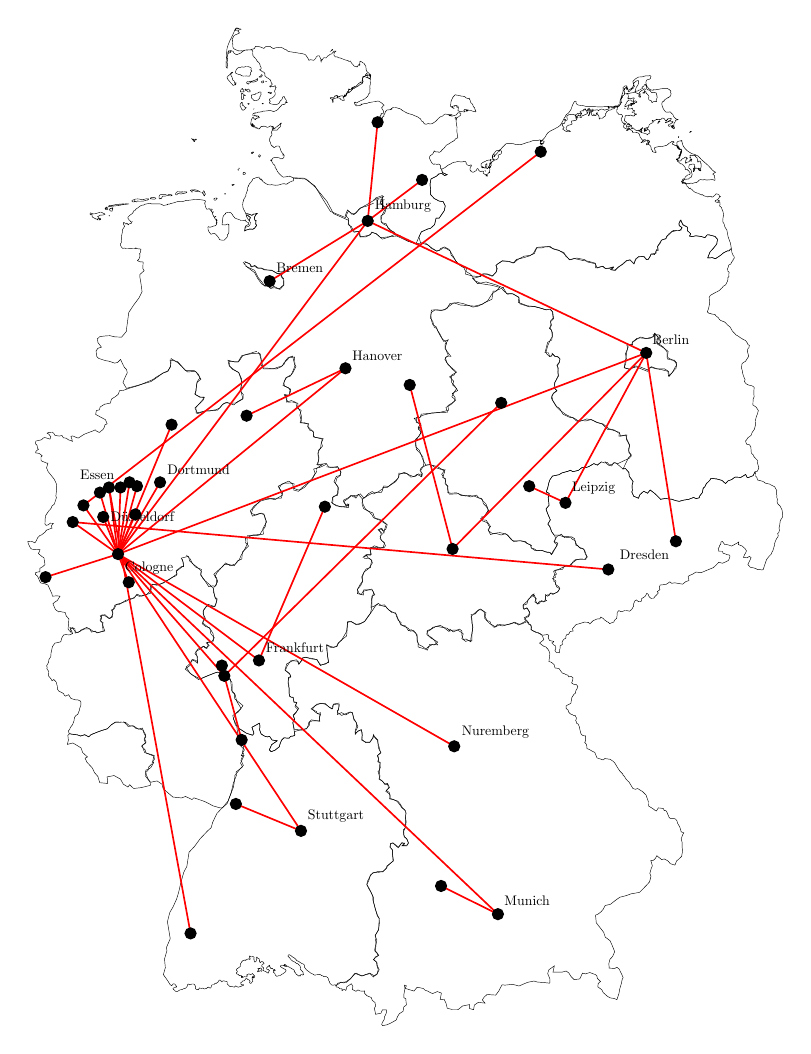
\begin{tikzpicture}

\definecolor{darkgray176}{RGB}{176,176,176}

\begin{axis}[
hide x axis,
hide y axis,
tick align=outside,
tick pos=left,
x grid style={darkgray176},
xmin=5.41798591613775, xmax=15.4935913085937,
xtick style={color=black},
y grid style={darkgray176},
ymin=46.8806100845338, ymax=55.4458555221558,
ytick style={color=black},
width=\linewidth,
height=1.28\linewidth
]
\addplot [line width=0.16pt, black]
table {%
8.70837306976324 47.7155570983886
8.71268272399902 47.7060623168946
8.71873188018799 47.6989135742188
8.71139812469477 47.6942787170411
8.69994831085216 47.6980361938477
8.69212532043457 47.6993370056152
8.68490028381348 47.6944847106934
8.67888832092291 47.6914443969727
8.66709423065197 47.6902580261231
8.66470623016357 47.6931343078614
8.66127586364757 47.6956634521484
8.66714191436779 47.6972236633302
8.67325878143305 47.6996383666992
8.67633533477795 47.705909729004
8.67048358917236 47.7113990783691
8.66622734069836 47.7148742675782
8.67177963256836 47.7169189453126
8.68023490905762 47.7178802490236
8.68641281127941 47.7136421203613
8.69133853912354 47.7165451049806
8.7006978988648 47.720142364502
8.70837306976324 47.7155570983886
};
\addplot [line width=0.16pt, black]
table {%
9.65046024322515 49.7763404846192
9.64671993255615 49.7352600097657
9.63594913482672 49.723991394043
9.63150024414062 49.6978416442872
9.68196868896479 49.7130584716797
9.734221458435 49.6947593688966
9.79042911529547 49.7175102233886
9.81357955932623 49.7102394104005
9.83292961120611 49.6546211242676
9.86216926574713 49.6362915039064
9.863450050354 49.6029090881348
9.84764003753668 49.5694007873536
9.84862041473389 49.5434799194336
9.88179874420172 49.5697097778321
9.92138957977306 49.5774688720703
9.93358993530279 49.5553703308107
9.9292192459107 49.5183410644531
9.92999839782721 49.4961585998536
9.98171043396007 49.4818916320802
10.0272397994996 49.4823112487794
10.0602989196777 49.5158119201661
10.0708284378052 49.5417518615723
10.0829687118531 49.5196914672852
10.1178789138795 49.4978485107423
10.1304388046265 49.4611091613771
10.1426296234131 49.4354286193848
10.1551504135133 49.3987312316896
10.1159391403199 49.3762817382813
10.1338491439819 49.3470115661622
10.1229391098022 49.3285102844239
10.1516275405884 49.3214416503906
10.1525583267212 49.2846908569336
10.1360483169556 49.2588005065918
10.1419305801392 49.2515106201172
10.1484308242798 49.2148399353028
10.1430997848511 49.1964187622071
10.1835393905641 49.1748085021974
10.2068395614625 49.1530303955078
10.2411603927612 49.1533889770509
10.2531890869142 49.1241607666016
10.2192888259888 49.0981292724609
10.2597303390504 49.0802116394044
10.2715091705323 49.0620002746582
10.271809577942 49.0436820983887
10.3179388046265 49.0331687927246
10.3584299087525 49.0189399719239
10.3934898376466 48.9899787902833
10.4167490005493 48.9682197570801
10.4391298294067 48.9606819152832
10.4558286666871 48.9457702636719
10.4669189453125 48.9272117614747
10.4555187225343 48.8977584838868
10.4665498733522 48.8644218444825
10.4607086181642 48.8238410949708
10.4493999481202 48.8091697692872
10.4437198638917 48.7981414794922
10.4323701858521 48.7760810852051
10.4378900527954 48.7575607299805
10.4490718841552 48.7426719665527
10.4770889282227 48.7239418029786
10.4938383102417 48.6941986083985
10.4712591171265 48.672248840332
10.4318799972534 48.6726303100586
10.4488496780395 48.6946296691895
10.4094686508179 48.6950187683105
10.3698692321777 48.6584815979004
10.3020696640015 48.6958007812501
10.2734708786012 48.6883697509767
10.2792100906373 48.6590385437012
10.301968574524 48.6369400024414
10.3018493652345 48.5963897705079
10.3073301315308 48.555690765381
10.2505998611451 48.5231018066407
10.2335996627809 48.5157890319825
10.2225599288942 48.4969596862794
10.1835803985596 48.4701118469238
10.1218395233155 48.4724998474122
10.0602903366089 48.4601097106934
10.0324802398682 48.4410095214843
9.99945068359381 48.3995895385743
9.98865890502935 48.3734092712402
10.011589050293 48.3403892517091
10.0457096099855 48.303810119629
10.0685291290284 48.2706718444825
10.0689191818237 48.2408599853516
10.0919904708862 48.1777496337892
10.1203107833863 48.1295204162598
10.1427507400513 48.1035804748536
10.1429491043091 48.0811614990234
10.1324081420899 48.0175285339355
10.0884895324708 47.9722709655763
10.110899925232 47.9388694763185
10.1001195907593 47.9014015197754
10.0948390960694 47.8639602661133
10.0949506759645 47.8452796936035
10.1060085296631 47.8416404724121
10.1281871795655 47.8156509399414
10.0951404571534 47.8078689575196
10.0731897354125 47.7852210998535
10.111780166626 47.7630691528321
10.1173086166382 47.7368392944336
10.1394691467285 47.7070999145508
10.1118392944337 47.6692314147949
10.0785303115844 47.6573905944824
10.0730514526367 47.6611213684083
10.0240898132324 47.6799316406251
9.97525978088385 47.6687393188477
9.92632865905762 47.6574096679688
9.84401988983154 47.6790313720703
9.81698989868164 47.6564903259277
9.78452968597423 47.6338920593263
9.74108982086193 47.6147994995117
9.70850086212164 47.6031799316406
9.67553997039806 47.6100387573242
9.64301013946533 47.5943489074708
9.61582946777344 47.5823020935059
9.60809707641602 47.5875549316407
9.59931564331055 47.5886344909669
9.59156322479254 47.5874824523926
9.58055114746094 47.5858955383301
9.56746578216564 47.5864715576173
9.55880260467541 47.5887489318848
9.55422782897955 47.591781616211
9.54609680175787 47.5974426269531
9.53862190246582 47.6039581298829
9.53589153289806 47.6126098632814
9.53309917449951 47.6181373596191
9.52856636047369 47.6193656921388
9.52529335021973 47.6254386901856
9.52381896972668 47.629135131836
9.52054023742676 47.6396560668946
9.51149272918713 47.6456222534181
9.50139141082775 47.6514587402344
9.48963165283209 47.6528053283691
9.48559665679932 47.6519966125489
9.4783754348756 47.6528930664062
9.47086143493658 47.651683807373
9.46423339843756 47.6545143127441
9.45750808715826 47.6581802368165
9.44812011718761 47.659523010254
9.43903255462652 47.6610946655273
9.42863941192627 47.6671295166016
9.42107486724848 47.6689834594727
9.4103507995606 47.6703491210938
9.39669227600092 47.6690368652344
9.39076995849609 47.6675834655762
9.3746967315675 47.6669807434082
9.36424160003662 47.6638488769532
9.35340976715088 47.664867401123
9.34339332580572 47.668212890625
9.33466625213634 47.6726226806641
9.32297325134272 47.6757583618165
9.31399726867681 47.6776199340821
9.30723381042486 47.6811218261718
9.29708385467535 47.6851539611817
9.29158020019531 47.689064025879
9.28154468536371 47.6937446594239
9.26723480224615 47.6994667053223
9.25749015808117 47.7048988342285
9.25014114379888 47.7104835510254
9.24290466308588 47.7170372009278
9.23632717132574 47.7226371765137
9.23141384124767 47.7293014526368
9.23014163970942 47.7369461059571
9.23065662384033 47.7432098388672
9.22443294525146 47.7482109069824
9.2136049270631 47.7519302368164
9.20805168151861 47.7532234191895
9.20123672485346 47.7544631958008
9.19145011901861 47.7590599060059
9.18303108215343 47.7624626159669
9.17338562011724 47.7661933898926
9.16315460205089 47.7707443237306
9.15264892578136 47.7739028930665
9.14535617828375 47.7753715515137
9.13589954376221 47.7795181274415
9.13059806823736 47.7854080200196
9.12322807312023 47.7908782958985
9.11534500122082 47.7942619323731
9.10388755798346 47.8007392883301
9.09918880462652 47.8025970458986
9.09108543395996 47.8041038513184
9.08247089385986 47.8089294433594
9.0749311447143 47.8122177124023
9.07011222839355 47.8168601989746
9.05317878723139 47.8216400146486
9.0467987060548 47.8235092163087
9.04012203216547 47.8222045898438
9.03320407867437 47.8167381286622
9.03183364868175 47.8129463195801
9.03997707366943 47.8063850402832
9.04921340942377 47.8014678955079
9.05444812774658 47.7963714599609
9.06152534484875 47.7916717529297
9.06891536712658 47.7852935791016
9.07866191864019 47.779483795166
9.08832454681402 47.7744712829591
9.09452724456787 47.7718505859376
9.1033754348756 47.7694129943848
9.11176872253429 47.7672576904297
9.12090778350841 47.7643127441406
9.12673091888422 47.7603073120117
9.13243103027355 47.7562713623046
9.13851070404064 47.7539863586426
9.15197944641108 47.7531929016113
9.15660190582281 47.7489128112794
9.1696834564209 47.7415885925294
9.17700290679932 47.7377548217775
9.17987060546881 47.7334213256836
9.18145370483398 47.7278709411622
9.18323516845703 47.723014831543
9.18505859375011 47.7189559936523
9.18371582031256 47.7103919982911
9.18822574615479 47.7066345214845
9.19218921661383 47.7022895812989
9.20068073272699 47.6975593566895
9.21247482299799 47.6903038024903
9.21541595458996 47.6844253540039
9.21637821197521 47.6759376525879
9.2215576171875 47.6689567565919
9.21742343902588 47.6667251586915
9.21097278594965 47.6650924682618
9.20100402832031 47.6685295104981
9.18757057189947 47.6692504882814
9.18506145477295 47.6643333435059
9.18147659301763 47.6574096679688
9.17087745666504 47.6605148315431
9.16667747497564 47.6618881225586
9.16502189636242 47.6571922302246
9.15844345092779 47.6579513549805
9.15294647216797 47.6605720520021
9.14853286743175 47.6659393310547
9.13695621490484 47.6681976318359
9.13035774230963 47.672836303711
9.12495899200434 47.6801300048829
9.11803817749035 47.6869888305665
9.11036586761475 47.688461303711
9.10772037506104 47.6919555664064
9.11163139343256 47.6946105957032
9.10950660705566 47.6994132995606
9.10383987426763 47.7048873901368
9.09731960296642 47.7083930969239
9.08959770202642 47.7112808227539
9.08130836486822 47.7134933471681
9.07031917572021 47.7178497314454
9.06135559082031 47.7216835021973
9.05045032501221 47.7261543273926
9.04244804382324 47.7277336120607
9.03370380401617 47.7314605712892
9.02359199523937 47.7336387634278
9.0131950378418 47.7391738891602
9.00182247161865 47.7456588745117
8.99239635467529 47.7479782104493
8.98550701141357 47.7454147338867
8.98817157745373 47.7411727905275
8.99635124206549 47.738452911377
9.0031938552857 47.7357177734375
9.01009559631348 47.731315612793
8.99729061126715 47.7321701049805
8.98511028289789 47.7368774414062
8.97660160064703 47.7398071289063
8.96861362457287 47.7408981323243
8.95772552490246 47.7418823242188
8.95046997070324 47.7406311035156
8.94417381286615 47.7381248474121
8.94136524200445 47.7318229675293
8.94789314270014 47.7273674011232
8.95422363281256 47.7254943847657
8.96321487426758 47.7214126586914
8.97292327880865 47.7169494628907
8.97875118255615 47.7149810791016
8.98491859436035 47.7132148742677
8.99152565002453 47.7115745544434
8.99672508239752 47.7102661132814
9.00337696075445 47.7057037353517
9.00872898101807 47.7000312805176
9.00550270080566 47.6943664550782
8.99800872802729 47.6882476806641
8.99105644226086 47.6840248107911
8.98582363128662 47.6820831298828
8.9809455871582 47.6804008483888
8.9737167358399 47.6746253967286
8.96322441101086 47.6727447509766
8.95596313476568 47.6699180603028
8.94959831237799 47.6669654846191
8.94071388244635 47.661678314209
8.92500972747808 47.6613731384278
8.91370391845697 47.6579627990723
8.90520191192638 47.6567687988281
8.89183425903332 47.6552238464357
8.87854003906256 47.6658515930176
8.87299537658691 47.6762657165527
8.86657619476318 47.6817436218263
8.860016822815 47.6839294433595
8.8548383712768 47.6879997253419
8.85904026031494 47.6944732666015
8.85572910308832 47.6989555358886
8.85916233062738 47.7020797729493
8.86531639099127 47.7003784179689
8.86726093292248 47.6974258422852
8.87013912200939 47.6968231201172
8.87787246704107 47.6989212036133
8.87658691406256 47.7021064758301
8.87370681762707 47.7049293518066
8.87209320068371 47.7085342407228
8.8550767898559 47.7081947326661
8.84860324859625 47.7121810913087
8.84465408325201 47.7162895202638
8.83664035797131 47.7179412841796
8.82831192016613 47.7151031494141
8.82244777679455 47.7168884277344
8.82460021972668 47.7212753295899
8.82076835632319 47.7217826843262
8.81555271148682 47.7270812988282
8.80809402465832 47.7294616699219
8.81241321563721 47.7334556579591
8.81119728088379 47.7357864379883
8.80929374694836 47.740249633789
8.80632114410412 47.7417984008789
8.79995632171642 47.7387847900391
8.79578304290783 47.7325515747071
8.78918266296392 47.7320938110352
8.78331184387207 47.7271347045898
8.77269458770752 47.7218818664551
8.77110385894775 47.7186965942382
8.77216911315918 47.7119445800782
8.78043079376226 47.7097396850585
8.79748630523687 47.7072372436525
8.79992485046398 47.7030181884767
8.80505752563488 47.7002639770508
8.80853271484381 47.6978797912598
8.80264472961431 47.69637298584
8.79735946655279 47.6904220581056
8.79629611968994 47.6814765930176
8.79178714752209 47.6793975830079
8.78179740905773 47.6826667785645
8.77375507354742 47.6864814758301
8.76686096191406 47.6908988952638
8.75304985046381 47.6949806213379
8.73966598510742 47.6966819763184
8.72960376739502 47.7051963806153
8.73334026336664 47.7132644653321
8.73743343353266 47.7203712463379
8.73475837707525 47.7235221862794
8.72563266754162 47.7267379760742
8.71699523925793 47.7299385070801
8.7134313583374 47.7350196838379
8.71482753753668 47.7417640686036
8.71932792663574 47.7455215454102
8.72465801239019 47.7497825622559
8.73334789276123 47.7511138916017
8.74229717254633 47.7527999877931
8.74053764343267 47.7580528259278
8.73138332366943 47.7633056640626
8.72906875610357 47.7671165466309
8.71936130523676 47.7701454162598
8.71004867553722 47.7696342468262
8.70104694366461 47.7657661437988
8.69786643981939 47.7621459960939
8.69301700592052 47.7624855041504
8.68807888031006 47.7706794738769
8.68549633026123 47.7755165100098
8.68839740753174 47.7802963256837
8.68372154235846 47.7855491638183
8.68181514739996 47.7921981811523
8.67188072204596 47.793399810791
8.66308689117426 47.7966003417969
8.66181182861334 47.8009719848633
8.65870666503906 47.8051910400391
8.65114688873291 47.8051300048828
8.64780712127691 47.7999229431152
8.64606094360352 47.7959175109863
8.64925193786632 47.7908935546876
8.64937305450445 47.7808074951172
8.64617824554449 47.7741088867188
8.64328956603998 47.771224975586
8.64021873474127 47.7699737548829
8.63050937652588 47.7657737731934
8.62617301940929 47.7697601318361
8.62173557281494 47.7739295959473
8.62348842620855 47.7819099426271
8.62011241912847 47.7851753234863
8.61669158935558 47.7901153564454
8.61961269378662 47.7944793701172
8.62158775329601 47.8017196655273
8.61474895477295 47.8076362609864
8.60294437408453 47.8091011047364
8.59474372863775 47.8063049316406
8.59028244018566 47.8076667785646
8.58341407775879 47.8077354431152
8.57697010040278 47.8070449829102
8.57386779785156 47.8120498657227
8.5686759948731 47.8143997192384
8.56313991546631 47.8113059997558
8.56232833862305 47.7999725341797
8.56805992126465 47.7970008850097
8.57480812072748 47.7928314208985
8.57164669036877 47.7875518798828
8.56379985809326 47.7875175476074
8.55491924285894 47.7910957336426
8.5483484268189 47.7901306152344
8.53843688964849 47.7880249023438
8.52550315856928 47.7843322753906
8.52108097076422 47.778305053711
8.51064491271978 47.7829437255861
8.50574398040771 47.7810249328613
8.49781322479248 47.7789306640626
8.49124526977545 47.7793998718263
8.48542690277111 47.778175354004
8.47800254821772 47.7733230590821
8.47058391571051 47.7679901123047
8.46823215484619 47.7631912231445
8.46524238586431 47.759693145752
8.45897006988537 47.757610321045
8.45654582977306 47.7513618469239
8.45364570617687 47.7474555969238
8.45261192321789 47.7400283813478
8.45591640472406 47.7332649230958
8.44421100616466 47.727840423584
8.44092559814453 47.7240943908693
8.43522071838379 47.723545074463
8.42614078521734 47.718246459961
8.41727733612055 47.7165603637696
8.4077291488648 47.7081985473634
8.40561485290533 47.7034225463868
8.41038513183594 47.7012672424316
8.41483974456793 47.6950988769531
8.41806221008301 47.690773010254
8.41506671905518 47.6867370605469
8.40631771087641 47.6838836669922
8.40472316741949 47.6787452697753
8.41301155090343 47.6720390319825
8.42396926879894 47.6713371276855
8.43025398254395 47.6682739257813
8.43540000915533 47.6643829345703
8.44223690032959 47.6607704162599
8.45190620422369 47.6595458984376
8.46172237396246 47.6596946716309
8.46718406677246 47.6611022949218
8.4658727645874 47.6533050537109
8.46818065643322 47.6453437805177
8.47563457489025 47.6434135437013
8.47862529754644 47.6453018188477
8.47322654724132 47.6467018127441
8.47423934936529 47.6486663818361
8.47744941711431 47.6503562927246
8.47510719299316 47.6544380187989
8.48215579986572 47.6535263061523
8.48421001434338 47.6495628356933
8.48891162872314 47.6482238769532
8.49495410919184 47.6478042602539
8.49670696258551 47.6515541076661
8.50172328948975 47.6520919799806
8.52180194854748 47.6509819030762
8.53375244140619 47.651035308838
8.53589725494385 47.6544456481934
8.5318603515625 47.6618843078614
8.5327262878418 47.6667861938478
8.53828525543219 47.663917541504
8.54125499725336 47.6647453308106
8.54394912719721 47.6703720092774
8.56136226654064 47.674674987793
8.57065582275396 47.6691246032715
8.57901000976562 47.6675910949708
8.58792495727545 47.6708793640138
8.59741973876964 47.6745796203613
8.60257434844971 47.6769714355469
8.61126804351807 47.6683006286621
8.61979579925537 47.6639213562012
8.62553977966314 47.6598205566406
8.6293888092041 47.6535186767578
8.6250953674317 47.6458625793458
8.61572360992437 47.6416931152344
8.60432529449474 47.64315032959
8.60906410217291 47.6462898254396
8.61533355712902 47.6501846313478
8.61017990112305 47.6560173034669
8.60499000549316 47.6551628112794
8.59684658050548 47.6471939086914
8.59804725646984 47.6345481872559
8.60279464721685 47.6254615783692
8.60586929321295 47.6168937683107
8.59806728363037 47.6113128662109
8.59033775329601 47.6057624816895
8.58634185791027 47.6028289794922
8.58178424835205 47.5997772216797
8.57199287414551 47.6011924743653
8.56536293029791 47.609031677246
8.5719194412232 47.6148300170899
8.57200813293457 47.6178207397461
8.56497573852539 47.6212997436523
8.55906963348389 47.6276054382325
8.54800891876221 47.6295013427734
8.54068088531494 47.631519317627
8.53899097442638 47.6347961425781
8.53183078765881 47.636344909668
8.52302646636969 47.6379623413087
8.51887035369879 47.6365852355956
8.51397514343267 47.6293640136719
8.50899219512945 47.6270828247071
8.50658226013195 47.6221199035645
8.49603366851807 47.6191177368165
8.48259353637695 47.618637084961
8.47723865509033 47.6142082214356
8.47123908996576 47.6092948913575
8.46470355987549 47.6075019836426
8.45824337005615 47.6053199768066
8.45950031280518 47.6011848449708
8.46142673492437 47.5941162109376
8.46748924255382 47.5896759033204
8.47150897979731 47.5885543823243
8.48195743560791 47.5894660949708
8.49204444885254 47.5909423828125
8.48968315124512 47.582763671875
8.47814178466803 47.581356048584
8.47262668609625 47.5788688659669
8.45789909362799 47.5765266418457
8.44715595245361 47.5738372802735
8.43453121185314 47.5713272094727
8.42343139648443 47.5707511901857
8.41617393493664 47.5744094848633
8.40685558319092 47.577709197998
8.39744186401379 47.580150604248
8.38742160797125 47.5745353698731
8.38315677642822 47.5703124999999
8.37329864501964 47.5716209411622
8.35743618011486 47.5742416381837
8.33047389984131 47.5747642517091
8.32132053375244 47.5784606933595
8.31454944610596 47.5834808349609
8.29977798461925 47.5913276672364
8.29470157623297 47.5965003967286
8.29558563232422 47.6082000732422
8.29330921173107 47.6126823425294
8.28142738342297 47.6163368225099
8.27288818359375 47.6161689758302
8.26095867156988 47.6178894042969
8.25420379638672 47.620059967041
8.24035167694092 47.6181640625001
8.23482704162603 47.6162605285645
8.22952365875256 47.6115531921388
8.22291278839117 47.6130638122559
8.21815490722656 47.622573852539
8.2067956924439 47.6262550354005
8.19632816314709 47.6241264343262
8.18986892700201 47.6179962158203
8.18776798248302 47.6148719787598
8.18297386169434 47.6098442077638
8.1759462356568 47.6084938049318
8.17027664184582 47.6041145324708
8.16212463378912 47.5996131896973
8.15146446228022 47.6012763977052
8.14140129089355 47.5982208251953
8.13720417022705 47.5918617248536
8.13370609283453 47.5890541076661
8.11497402191168 47.5892066955567
8.10432720184326 47.5844078063965
8.10028171539307 47.5709686279297
8.09580707550049 47.5655212402345
8.08651161193859 47.5628051757813
8.07672309875494 47.5660247802735
8.0710134506225 47.5700035095216
8.06526947021496 47.569881439209
8.05796813964849 47.5688858032227
8.04987525939953 47.5635643005371
8.03913402557379 47.5593109130859
8.01532363891607 47.5568771362305
8.00687599182135 47.5593643188477
7.9995379447937 47.5624160766602
7.98657608032238 47.5614891052246
7.97047805786133 47.5616455078126
7.9571299552918 47.56400680542
7.95049285888666 47.5555419921876
7.94698715209961 47.5500297546387
7.93535804748541 47.5523071289063
7.91738605499279 47.5539131164551
7.90874481201172 47.5603256225587
7.90722417831415 47.5685386657715
7.91026782989508 47.5759582519532
7.90484380722052 47.5839538574219
7.89448404312134 47.5920257568361
7.88652515411371 47.5948944091798
7.86763381958008 47.5952033996581
7.85302877426147 47.5913429260255
7.84006214141851 47.5888862609864
7.83285522460938 47.5925521850587
7.82077217102056 47.5946998596192
7.81562089920044 47.5909194946289
7.8118138313294 47.5827026367187
7.80856800079346 47.5754699707031
7.80025911331177 47.5706901550294
7.79436206817638 47.5646133422852
7.78735065460205 47.5618591308595
7.77046012878424 47.5591278076172
7.75716018676769 47.5557289123535
7.75042819976801 47.5516777038575
7.72458600997925 47.5497512817383
7.70842981338501 47.5442657470704
7.69653606414795 47.5389595031738
7.68693876266479 47.5361022949219
7.66517782211309 47.538833618164
7.6569390296936 47.5460662841798
7.65017890930176 47.5495491027833
7.64268398284912 47.5519828796387
7.63682699203503 47.5587043762208
7.63945198059076 47.5631065368653
7.64800930023193 47.56498336792
7.66280603408825 47.5679054260255
7.6720399856568 47.5717277526857
7.67832088470459 47.5705413818359
7.68170309066772 47.5735359191895
7.67740488052362 47.5763473510743
7.67208814620966 47.5850105285645
7.66676616668701 47.5863838195802
7.6645069122315 47.5893058776855
7.65889120101934 47.5940628051758
7.64944601058954 47.5961647033691
7.63876819610596 47.5969467163087
7.63531112670898 47.5926742553711
7.62842178344721 47.5879516601563
7.62015104293823 47.5820465087891
7.60277509689337 47.5896835327149
7.57183313369745 47.6214981079102
7.52001142501837 47.6680755615235
7.5438866615296 47.7225837707521
7.53389596939093 47.7902183532715
7.56260490417486 47.853084564209
7.55832004547131 47.8812789916993
7.60334253311157 47.9485626220703
7.56931543350231 48.0806770324707
7.58777141571039 48.1280059814454
7.59949970245361 48.1556320190431
7.63713073730469 48.195873260498
7.68145990371715 48.2596397399903
7.70507860183727 48.3096351623536
7.73096609115606 48.3822059631348
7.76616191864014 48.4639739990235
7.80516195297247 48.5135002136231
7.83175373077404 48.6232795715332
7.8962516784668 48.6672096252442
7.96770238876343 48.7297859191895
8.01622200012213 48.7623977661132
8.05623722076416 48.7896461486816
8.10069656372065 48.8154487609864
8.11810111999506 48.8563079833984
8.16850566864019 48.9245033264161
8.23029518127453 48.9672966003419
8.2952995300293 49.0041503906251
8.3408002853393 49.0840110778809
8.36952018737793 49.1632385253907
8.40528869628912 49.2203521728515
8.40367889404291 49.2499122619629
8.48058891296392 49.289821624756
8.45673084259039 49.3183708190919
8.49954032897961 49.3787803649902
8.46553993225098 49.3775291442872
8.50355815887451 49.4229621887208
8.44516944885254 49.4612503051757
8.44361877441412 49.501579284668
8.44622039794922 49.5861892700195
8.5276603698731 49.5521697998047
8.60262966156006 49.5363311767579
8.61937904357916 49.5515289306641
8.59504890441895 49.5983886718749
8.68616867065435 49.6305313110352
8.69249820709229 49.6087417602539
8.68750858306879 49.5793113708497
8.70555973052984 49.5469322204591
8.74616146087658 49.529811859131
8.78079032897955 49.5234107971192
8.80945873260498 49.527759552002
8.83880996704113 49.4992408752442
8.90242958068853 49.4930992126465
8.86804866790783 49.4779396057128
8.83375930786138 49.4626922607422
8.80581855773926 49.4220085144044
8.82904815673828 49.4079818725587
8.87488937377924 49.4197616577149
8.92646980285656 49.4459686279298
8.93756866455078 49.4716491699219
8.95446014404308 49.4974212646485
8.9830493927002 49.5160217285156
9.04674911499023 49.5128517150878
9.06380844116217 49.527629852295
9.1041898727417 49.5314521789551
9.11559867858898 49.5388298034668
9.10931968688976 49.5645904541017
9.18978977203375 49.5793418884278
9.25874996185303 49.5864486694337
9.27552032470697 49.6085815429688
9.28634071350103 49.6381416320802
9.31462955474865 49.6565589904786
9.41805934906012 49.6452293395996
9.41161823272716 49.6711921691895
9.4280300140382 49.6971321105957
9.39357852935802 49.7045593261719
9.35892868042004 49.7193984985352
9.34142971038824 49.7342185974122
9.31266880035406 49.7416610717773
9.36345958709722 49.767520904541
9.43115901947021 49.7861289978028
9.48233985900879 49.77885055542
9.51671981811523 49.7641105651855
9.56256961822521 49.7420196533203
9.58343982696545 49.7794418334961
9.65565872192388 49.7875595092775
};
\addplot [line width=0.16pt, black]
table {%
10.1338596343995 50.5499992370606
10.175030708313 50.5463218688965
10.2220582962036 50.5388488769532
10.25749874115 50.5127105712891
10.3105001449586 50.4940490722657
10.3458290100097 50.4828720092773
10.3696393966674 50.4418487548828
10.3815002441407 50.4269409179687
10.3933992385864 50.4082794189453
10.4287796020508 50.3896713256837
10.4935398101807 50.3711090087891
10.5171899795533 50.3487510681153
10.5583114624024 50.3525505065919
10.5996913909913 50.3190307617188
10.5999088287354 50.2853622436525
10.605890274048 50.2666816711426
10.6177797317505 50.2442588806153
10.6647691726684 50.2294197082521
10.7230186462403 50.1997985839844
10.7518301010132 50.2447204589844
10.8093795776368 50.241310119629
10.8495798110962 50.2638320922853
10.8035392761232 50.2822418212891
10.7690296173095 50.2932815551758
10.7172508239746 50.322940826416
10.7224493026733 50.3526611328126
10.7798700332641 50.3675994873048
10.8199300765991 50.3825187683106
10.8772802352905 50.3937797546387
10.9118385314942 50.3827590942383
10.9868106842042 50.3459205627443
10.9981107711791 50.3644790649415
11.0385084152223 50.3423614501954
11.1132392883301 50.3648986816407
11.1421594619752 50.3501586914063
11.1421003341676 50.3167495727539
11.1596403121949 50.2834587097168
11.1940393447877 50.2872505187988
11.2516689300537 50.2651901245118
11.2518787384034 50.2911415100098
11.2640590667726 50.3320198059083
11.2763004302979 50.3803787231446
11.2649793624878 50.4100494384766
11.2652893066406 50.4397888183594
11.2540006637574 50.4806289672852
11.3007707595826 50.480812072754
11.347978591919 50.5144386291504
11.3831501007081 50.514560699463
11.4180603027344 50.492359161377
11.4175081253052 50.4514503479003
11.4523401260377 50.4254989624024
11.4814081192017 50.4069709777833
11.5165004730225 50.395881652832
11.5514888763429 50.3810615539552
11.5987586975097 50.3997993469238
11.6690998077392 50.3962516784669
11.7279195785524 50.4038391113282
11.763279914856 50.4113807678224
11.781060218811 50.4188995361329
11.8332996368409 50.4041213989258
11.8683385848998 50.4042091369629
11.9332876205445 50.4230957031251
11.9508810043336 50.4051361083985
11.9728994369507 50.40087890625
11.988410949707 50.3786888122559
11.980833053589 50.3621330261232
11.9984741210938 50.3524780273438
12.042724609375 50.337890625
12.0652704238892 50.3379096984864
12.0980758666992 50.3269500732423
12.1192445755005 50.3130340576173
12.1273336410524 50.2997283935546
12.1371698379517 50.2821121215821
12.0858602523804 50.2553520202638
12.1089019775391 50.2439460754395
12.1319217681885 50.2320747375489
12.161280632019 50.2252082824708
12.1852025985718 50.2088623046876
12.1989192962646 50.1956214904786
12.2102556228639 50.171459197998
12.1990604400635 50.1118202209473
12.2236337661744 50.1068382263184
12.2387990951538 50.1005210876465
12.2619924545289 50.087646484375
12.2671489715576 50.074031829834
12.2734403610229 50.0612945556642
12.3019199371339 50.058864593506
12.3234615325928 50.0559158325196
12.3403053283693 50.0390205383301
12.3644390106201 50.0203819274903
12.3873596191406 50.0163803100587
12.4103908538818 50.0084609985353
12.4300937652589 50.0047760009766
12.4392223358154 49.9918441772462
12.4683113098146 49.9958801269531
12.4915103912355 49.9839515686036
12.4858713150024 49.9634895324708
12.474949836731 49.9445724487304
12.4975881576538 49.9344406127931
12.5331840515136 49.930633544922
12.5491809844971 49.9181823730469
12.5444335937501 49.9042472839355
12.526593208313 49.8848419189454
12.5192785263063 49.8639907836915
12.5033111572267 49.8559761047363
12.4783086776733 49.8320312500001
12.4698915481567 49.8037109375001
12.4658308029174 49.7857551574708
12.4473314285279 49.779411315918
12.4087495803834 49.7661895751954
12.4084739685059 49.7448501586915
12.4312286376953 49.7328186035157
12.4406900405884 49.7154693603517
12.4583139419557 49.7031402587891
12.4862108230591 49.6961135864258
12.4951152801514 49.6907997131347
12.516598701477 49.6916007995605
12.5329446792603 49.6718978881837
12.5283613204957 49.6570854187012
12.5227203369141 49.6488914489746
12.5303115844727 49.6449050903321
12.536660194397 49.6285514831544
12.5528450012207 49.6246528625488
12.55885887146 49.6174087524415
12.5703268051148 49.5979232788087
12.5753774642945 49.5801544189454
12.5844507217407 49.5536079406739
12.5942611694337 49.5408020019531
12.6154766082764 49.5331649780273
12.6458301544191 49.5310592651367
12.6443939208985 49.4944534301758
12.6328067779542 49.4800148010255
12.6467456817628 49.471939086914
12.6570024490356 49.4582099914551
12.6610746383668 49.4321670532227
12.6898450851441 49.4251441955566
12.7193031311036 49.4136276245117
12.7555837631226 49.4025840759278
12.7829885482788 49.3591842651368
12.8576192855836 49.3436088562013
12.8767499923707 49.3545112609864
12.9411487579346 49.3486595153809
12.9804162979126 49.3320274353027
13.0011110305786 49.3171577453613
13.0326108932496 49.282730102539
13.0609884262086 49.2558517456055
13.0954179763795 49.2338256835938
13.0999822616577 49.2223091125489
13.1145906448364 49.2165374755859
13.1311626434327 49.1972122192383
13.1542034149171 49.1806259155275
13.1691198349 49.1725578308107
13.1861791610718 49.1554489135743
13.2177381515503 49.1211318969728
13.2482128143311 49.1143608093263
13.2749977111816 49.1206436157227
13.3338308334351 49.0973205566407
13.3769292831421 49.0707321166993
13.4074516296388 49.0151824951172
13.4071636199951 48.9933280944824
13.4084062576295 48.9843482971191
13.4374084472656 48.9726219177247
13.4663915634155 48.9608879089355
13.4885816574097 48.9487113952637
13.5033550262451 48.9451217651367
13.5268354415895 48.9692535400391
13.5613679885865 48.9668998718262
13.5891103744508 48.9641113281251
13.5981464385987 48.9477691650392
13.6144990921021 48.9491691589357
13.6252593994141 48.9433708190918
13.634614944458 48.9307212829589
13.6433172225952 48.9167137145997
13.6576251983643 48.8959197998046
13.6675214767456 48.8887939453126
13.697340965271 48.8847885131837
13.72260761261 48.8853912353517
13.736798286438 48.8813133239747
13.7519311904907 48.8700218200685
13.7616329193116 48.847972869873
13.7695722579957 48.8394012451173
13.7775077819825 48.8308258056642
13.7888803482057 48.8169898986818
13.804204940796 48.7826385498047
13.8359575271606 48.7750511169435
13.8235597610474 48.7606811523437
13.8042993545533 48.7282905578614
13.8144683837891 48.7027778625489
13.8162641525269 48.660327911377
13.8200798034668 48.6297721862793
13.8099441528321 48.59090423584
13.7608966827392 48.5613784790039
13.7489957809449 48.5570755004883
13.7286520004272 48.522789001465
13.6723461151123 48.5339279174805
13.6453313827515 48.5543746948242
13.6019525527955 48.5706596374512
13.5657234191895 48.5662689208986
13.5085992813111 48.5963897705079
13.4908790588379 48.5746192932128
13.466835975647 48.5603561401368
13.435447692871 48.5598144531251
13.4545402526856 48.516300201416
13.4411983489991 48.4977531433105
13.4236793518068 48.4577789306642
13.437659263611 48.4363365173339
13.4201545715332 48.3915367126465
13.3686418533325 48.3558235168458
13.297986984253 48.3099098205566
13.1977338790894 48.2989654541016
13.1412687301636 48.2855300903321
13.058403968811 48.2717361450196
13.0034379959107 48.2465362548829
12.9463319778442 48.21732711792
12.8824644088746 48.2075424194337
12.8559894561769 48.1768112182618
12.8324937820435 48.1590919494629
12.7974910736085 48.1415252685548
12.7647256851196 48.1320304870606
12.7737283706666 48.0727195739747
12.8640136718749 47.9982185363769
12.8832569122315 47.960521697998
12.91832447052 47.9440841674805
12.942084312439 47.9312858581543
12.9666528701782 47.8963623046876
12.9973659515381 47.8474273681642
12.971534729004 47.809497833252
12.9376850128173 47.7854537963867
12.9261684417725 47.7532806396484
12.9307203292847 47.7189598083497
12.9976987838746 47.7162590026857
13.023491859436 47.7256660461425
13.05153465271 47.7115440368652
13.0790977478027 47.6757202148438
13.0995168685914 47.6454505920411
13.0879936218263 47.6294746398927
13.076530456543 47.5950012207032
13.0589895248414 47.5579109191895
13.048776626587 47.5206642150879
13.0242395401 47.4727592468262
12.9931430816652 47.4817504882814
12.9473209381104 47.4861221313477
12.9130592346192 47.4967422485352
12.857219696045 47.5283584594727
12.8396644592286 47.5513954162598
12.7920913696288 47.572364807129
12.7970190048219 47.5989112854004
12.8250036239625 47.6143913269044
12.7875633239747 47.6385955810546
12.7791461944581 47.6621894836426
12.756314277649 47.670021057129
12.6943368911743 47.6846656799316
12.6443052291871 47.6741828918457
12.6053342819214 47.6792488098145
12.5741014480591 47.6348838806152
12.5056247711183 47.6290473937989
12.4667396545411 47.6541442871094
12.4402570724487 47.6813812255859
12.4086751937867 47.6962356567383
12.3621530532838 47.6880836486816
12.2970485687257 47.6876602172852
12.2479887008668 47.6875000000001
12.2648983001709 47.7364311218262
12.1988801956177 47.7064285278321
12.1838417053223 47.6771430969239
12.2121057510375 47.6326789855958
12.2092800140381 47.6012001037598
12.1544904708863 47.6053619384767
12.0608491897584 47.6101417541504
12.0168094635009 47.618049621582
11.9396581649781 47.6077308654786
11.8348293304444 47.5792884826661
11.7907781600952 47.5871620178224
11.7553968429565 47.5922279357911
11.6676912307739 47.5862731933595
11.6300992965699 47.5884780883789
11.608759880066 47.5632514953614
11.5926008224488 47.5417556762695
11.5534496307373 47.5084190368652
11.4484786987305 47.5131607055665
11.4125556945802 47.4922332763672
11.3905820846558 47.4707946777344
11.4240808486939 47.4456214904786
11.3416061401367 47.4518241882324
11.2938966751099 47.4301986694337
11.2849788665772 47.3948822021484
11.2355899810791 47.4031791687012
11.2359476089478 47.434196472168
11.1511888504028 47.4235649108887
11.0972509384155 47.3957214355469
11.0232343673707 47.3962020874023
10.9648666381835 47.4060363769532
10.9496288299561 47.4460220336915
10.9265918731689 47.4762153625488
10.8790102005005 47.4740905761719
10.8887186050416 47.5056991577148
10.8941373825074 47.5243263244629
10.845311164856 47.5358276367188
10.7874727249146 47.5203704833984
10.7612400054932 47.5273323059082
10.7269411087036 47.5400238037109
10.6975908279419 47.5456695556642
10.6754474639893 47.5601463317871
10.599970817566 47.5698318481446
10.5791826248169 47.5540237426758
10.5614671707154 47.5397911071778
10.453429222107 47.5610198974609
10.4698295593262 47.5809860229492
10.4459648132324 47.5856666564941
10.4517965316772 47.5575599670411
10.4396677017212 47.5170974731445
10.4384460449219 47.4881553649903
10.4626731872559 47.4797286987305
10.4648036956788 47.4579162597657
10.4700441360474 47.43265914917
10.4349317550659 47.4137001037598
10.4302892684937 47.3823738098145
10.3843297958375 47.3636360168458
10.3621091842652 47.3408699035645
10.3452501296998 47.3139190673829
10.2851896286011 47.2917213439943
10.2363986968995 47.2772216796876
10.1813392639161 47.2699394226075
10.1692867279053 47.2791099548341
10.1761407852174 47.2925491333009
10.2038888931274 47.3231086730958
10.2019653320312 47.3358116149902
10.2262201309204 47.3686408996582
10.2268695831299 47.3929176330567
10.178505897522 47.3934936523437
10.1606607437134 47.3672485351563
10.0961999893189 47.3585090637207
10.0808954238892 47.4045257568361
10.0949831008912 47.4233703613282
10.0886058807373 47.4506454467774
10.0553798675537 47.466869354248
10.0433826446534 47.4893760681152
9.99119472503662 47.5032081604005
9.96118831634516 47.5230407714844
9.96367740631115 47.5411643981935
9.94481468200684 47.5389022827148
9.90803241729742 47.54056930542
9.88100242614757 47.5485458374025
9.85710906982422 47.5382194519043
9.81310176849371 47.5524559020997
9.82004165649414 47.5752944946289
9.8015394210816 47.5971603393556
9.74723911285395 47.5741691589357
9.73667144775402 47.5472412109375
9.73229598999023 47.5453567504883
9.72355270385748 47.5503120422364
9.70933628082275 47.5516967773438
9.70098495483398 47.5486297607422
9.6951141357423 47.5439605712892
9.68802356719971 47.5443000793457
9.68502902984631 47.547721862793
9.68946456909191 47.5498428344728
9.69080257415777 47.5552864074708
9.68641662597656 47.5583343505859
9.67394638061529 47.5574188232422
9.66531181335461 47.5581893920899
9.65615940094 47.5600166320801
9.65301132202154 47.5647773742676
9.64020729064953 47.5679283142089
9.6367712020874 47.5708465576173
9.63286781311035 47.5715637207032
9.62277412414551 47.570915222168
9.61513328552257 47.5761795043946
9.61192798614502 47.5812339782716
9.62124824523926 47.5862388610839
9.63741016387951 47.6017799377442
9.67562007904064 47.6063308715821
9.71927928924561 47.6107521057129
9.74122905731201 47.6073989868165
9.7954092025758 47.637722015381
9.82240962982183 47.660270690918
9.86045074462902 47.6791992187501
9.93178081512451 47.657440185547
9.98069953918468 47.6687507629395
10.0295095443726 47.6761589050294
10.0674896240234 47.6497421264649
10.0895986557007 47.6650619506837
10.1118097305298 47.6729621887208
10.1283702850342 47.7069396972656
10.1117887496948 47.7367897033691
10.1062688827515 47.7667694091796
10.0676794052124 47.7851715087891
10.1006603240967 47.8041801452637
10.1336984634399 47.8194389343262
10.1059894561769 47.8453788757325
10.089409828186 47.8489799499512
10.083830833435 47.8601303100587
10.1000576019287 47.9088706970215
10.0942192077638 47.9499092102052
10.093999862671 47.9760589599609
10.132378578186 48.0212707519531
10.137399673462 48.0811004638671
10.1371698379517 48.1072616577148
10.1147499084473 48.1294593811035
10.0919103622437 48.1852188110353
10.0632390975952 48.2482414245607
10.0628490447998 48.2780303955079
10.0400190353395 48.311149597168
10.011480331421 48.3478202819825
9.98871994018566 48.3697013854981
10.0161504745483 48.4073295593263
10.0324296951295 48.4447288513183
10.0658416748047 48.4639205932617
10.1275291442872 48.4652099609376
10.1835393905641 48.4738197326661
10.2281589508057 48.4970588684082
10.2392406463624 48.5158500671388
10.2562789916992 48.5267295837403
10.3129796981812 48.5556297302247
10.3018903732301 48.6074600219727
10.3019781112672 48.6406211853027
10.2677593231202 48.6626586914062
10.2791976928711 48.6920700073242
10.3077697753906 48.6958007812501
10.3755283355712 48.662109375
10.4151096343995 48.6986618041993
10.4432096481324 48.690990447998
10.4149894714356 48.6728019714357
10.4825496673585 48.6795310974121
10.4938497543336 48.6978912353517
10.4715013504029 48.7313690185547
10.443440437317 48.7427101135254
10.4379081726075 48.7612495422364
10.4379787445069 48.7760314941407
10.4324893951417 48.7982521057129
10.4550285339356 48.8091201782228
10.4607696533203 48.8349189758302
10.4609394073487 48.8644714355469
10.4555492401122 48.9014587402344
10.4557399749755 48.9309997558595
10.4558382034302 48.9494590759277
10.4335298538209 48.9607200622559
10.4167718887329 48.975570678711
10.3932991027833 49.0009803771973
10.3641099929811 49.0226593017579
10.312189102173 49.0331115722656
10.2661209106446 49.0399513244629
10.2713899612427 49.0693397521974
10.2595386505128 49.0912094116212
10.2249002456665 49.1055221557618
10.2645597457885 49.1279411315917
10.241008758545 49.1607208251953
10.2067699432374 49.1567001342773
10.1777496337891 49.1784210205078
10.1374588012695 49.1926918029786
10.1427192687988 49.214771270752
10.1247301101685 49.2550086975098
10.1417598724366 49.2588500976564
10.1409692764282 49.2919197082521
10.1515302658082 49.3251190185547
10.1228504180908 49.3321914672852
10.1336507797241 49.3543701171876
10.1215295791627 49.3800086975098
10.1608381271362 49.398780822754
10.1312484741212 49.4353294372559
10.1246318817138 49.4647407531739
10.1235790252686 49.4979019165039
10.0885486602783 49.5234298706054
10.0710792541504 49.5343589782716
10.0660009384156 49.5158615112305
10.0216703414918 49.4785690307618
9.97614860534674 49.478141784668
9.92974090576166 49.5035514831543
9.93437862396246 49.5331802368164
9.92776012420654 49.5590209960938
9.92124938964849 49.5811805725098
9.87067890167248 49.5621910095216
9.84847831726074 49.5471801757813
9.85333061218267 49.569450378418
9.88053894042963 49.6030616760253
9.85631942749029 49.6399612426759
9.83248996734613 49.6657600402833
9.8134298324585 49.7139587402345
9.7847194671632 49.7174720764161
9.72245979309076 49.7021217346191
9.68297863006603 49.6907005310059
9.63645935058594 49.7127990722657
9.63018035888678 49.7276687622071
9.64653968811029 49.7389907836914
9.65614891052257 49.7763710021973
9.58359909057629 49.775718688965
9.57377910614014 49.742099761963
9.52826023101801 49.7567405700685
9.48785972595221 49.7825813293457
9.4481601715089 49.7861709594727
9.38025856018078 49.7786407470703
9.32418823242188 49.7379417419434
9.34150981903082 49.7305297851564
9.37596988677984 49.7230911254884
9.3878698348999 49.7045593261719
9.42761993408209 49.7119598388672
9.41152000427246 49.6748886108398
9.41795921325678 49.648941040039
9.32625961303717 49.6491203308106
9.29208946228027 49.6381187438966
9.29259872436518 49.6159210205079
9.25866985321045 49.5901489257814
9.20138835906977 49.5755920410157
9.10894870758062 49.5830001831055
9.09056091308594 49.638069152832
9.11314868927002 49.663990020752
9.095290184021 49.6932792663574
9.12947940826416 49.715660095215
9.16348934173595 49.7453804016113
9.12269878387457 49.7708511352539
9.13959026336664 49.793140411377
9.10496044158941 49.7964401245117
9.09277820587158 49.8330993652344
9.06967926025402 49.8327713012696
9.05212974548334 49.8435592651368
9.04594039917004 49.865550994873
9.0451192855835 49.9097213745117
9.03853988647455 49.9501304626465
9.03779888153076 49.9869613647461
9.0667295455932 49.9948387145996
9.04866981506353 50.020320892334
8.99534988403326 50.0451011657715
9.01706981658941 50.0933685302734
9.08629035949713 50.1167907714845
9.15641021728521 50.1144485473633
9.16390991210949 50.0886993408204
9.19011974334728 50.1151008605958
9.21074867248535 50.1414108276367
9.25472927093506 50.1420822143555
9.3270692825318 50.1354217529297
9.38334083557123 50.1247901916504
9.43019962310802 50.0841522216798
9.49134922027594 50.0922393798828
9.52411937713617 50.1112403869629
9.50975990295422 50.1709213256837
9.5018396377564 50.2119789123536
9.50574874877935 50.2419319152833
9.54083824157715 50.2235412597657
9.58082962036133 50.2201499938965
9.63168907165533 50.2317810058595
9.64205932617199 50.2542686462402
9.6813898086549 50.2770004272462
9.74269866943359 50.3446617126465
9.75262928009045 50.4013519287111
9.75783920288086 50.4240913391114
9.80528926849371 50.4205894470215
9.86490917205822 50.4021797180176
9.91777992248529 50.4100494384766
9.96456813812267 50.425350189209
10.0109100341797 50.4668998718261
10.0400190353395 50.4933319091797
10.0985202789307 50.5498886108399
10.1220407485962 50.5574798583985
};
\addplot [line width=0.16pt, black]
table {%
13.1778898239136 52.3903198242189
13.1116189956665 52.4060821533204
13.131049156189 52.4354515075685
13.1387586593628 52.4761199951172
13.1280698776245 52.5133399963379
13.1606092453003 52.5647811889649
13.1554203033448 52.5871009826661
13.2162094116212 52.5825195312501
13.2110280990601 52.6048393249513
13.2671203613282 52.6337013244629
13.3099288940431 52.6367797851564
13.3889493942262 52.6319198608399
13.4317188262939 52.6349792480469
13.4688987731935 52.6492614746094
13.4819107055665 52.6675987243652
13.5293893814087 52.6409492492676
13.5148601531983 52.5892715454103
13.5924396514894 52.5584487915039
13.6457986831666 52.5316886901856
13.6378307342529 52.491039276123
13.6494197845459 52.4797401428223
13.7031803131104 52.4640808105469
13.7327003479003 52.4487915039062
13.749758720398 52.4262809753419
13.7243490219117 52.4007301330568
13.6986083984376 52.3677711486816
13.6488800048828 52.33890914917
13.6445589065553 52.3760299682618
13.5724582672119 52.3882598876954
13.4940395355225 52.3968620300294
13.4278287887574 52.4089622497558
13.3965196609497 52.3871803283693
13.3064098358155 52.4107208251954
13.2520475387573 52.4189109802246
13.1778898239136 52.3903198242189
};
\addplot [line width=0.16pt, black]
table {%
13.8795080184937 53.5010681152344
13.877610206604 53.4753189086914
13.9195804595947 53.4501190185547
13.9056997299195 53.431869506836
13.9367084503175 53.4276733398438
13.9811191558838 53.4341011047364
14.0438995361328 53.4290084838868
14.0920715332032 53.4195213317871
14.1210422515869 53.4420242309571
14.1400747299195 53.4417114257812
14.2150812149048 53.428997039795
14.2448511123658 53.4063415527344
14.2356176376343 53.3694801330568
14.1928892135621 53.3347053527833
14.1544790267945 53.3082885742188
14.1254091262819 53.2608604431153
14.1826286315919 53.2633819580078
14.22008228302 53.2553100585939
14.2791128158569 53.2800903320314
14.3189849853516 53.3016395568848
14.3644485473633 53.315731048584
14.383360862732 53.3154945373536
14.4036426544191 53.3312606811523
14.4146718978882 53.3305053710937
14.4194898605348 53.3036231994629
14.4366683959961 53.2785797119142
14.4441108703614 53.2744750976562
14.4489364624024 53.2622032165528
14.4469757080078 53.2565307617188
14.4357290267945 53.2514572143555
14.4339761734008 53.2423477172853
14.4135322570801 53.2265472412109
14.4077157974243 53.2141113281251
14.3913402557374 53.208625793457
14.3789186477662 53.204158782959
14.3740854263305 53.1853027343751
14.3671817779542 53.1800270080567
14.3702974319459 53.1579284667969
14.3864736557007 53.1491088867187
14.3812189102173 53.1313972473145
14.3825340270996 53.1150665283204
14.3714685440063 53.1083412170411
14.3704023361207 53.1002578735353
14.3711614608764 53.094596862793
14.3657941818237 53.0787239074708
14.3594961166383 53.0706787109376
14.345703125 53.0529174804688
14.3370170593262 53.047924041748
14.3191986083985 53.0417251586913
14.3116779327394 53.036849975586
14.2999544143678 53.0279808044434
14.2922525405883 53.0230712890625
14.2841176986695 53.0183601379394
14.2771921157836 53.0142860412598
14.2705068588257 53.0084838867189
14.2562665939331 53.0031661987306
14.2353305816651 52.9959945678711
14.2221813201904 52.9923706054688
14.1652574539185 52.9717826843263
14.1549119949341 52.9661254882813
14.1436986923218 52.9521484375
14.1474342346191 52.9252586364747
14.1500921249391 52.907341003418
14.136040687561 52.8655014038086
14.1214036941529 52.8400878906251
14.13827419281 52.8299674987793
14.1571197509766 52.8280410766602
14.1764841079711 52.8229522705078
14.2140712738038 52.8204040527344
14.2226886749268 52.811824798584
14.2361364364623 52.8034973144531
14.2546949386598 52.7954330444337
14.2664279937745 52.7824974060059
14.2815341949463 52.7742500305176
14.3030099868775 52.7681922912598
14.3260164260865 52.762996673584
14.3418741226196 52.7555961608887
14.3665161132813 52.7379837036133
14.3984079360962 52.7215461730958
14.4217691421508 52.6943588256837
14.436050415039 52.6828231811523
14.4570837020875 52.670337677002
14.4657154083252 52.6610145568848
14.4888896942139 52.6538772583008
14.5033798217773 52.6475410461427
14.5235509872438 52.6379356384278
14.5330085754396 52.6355094909669
14.5507392883302 52.6275215148927
14.5671510696412 52.6216468811035
14.5824460983276 52.6178855895996
14.5950746536255 52.6094779968262
14.6073713302613 52.5965423583986
14.6164283752441 52.5834426879883
14.6323041915894 52.5797080993652
14.6266088485718 52.5613746643066
14.6130361557007 52.551685333252
14.6077690124513 52.534824371338
14.6085472106935 52.5286674499512
14.6186885833741 52.5068283081055
14.624041557312 52.493553161621
14.6114587783814 52.4817085266114
14.5860900878907 52.4555587768556
14.5432081222535 52.4374885559083
14.5353088378907 52.4037895202638
14.5459909439087 52.3809204101563
14.5477228164673 52.3679237365724
14.5581426620483 52.3438148498536
14.5674667358398 52.3282775878907
14.5799093246461 52.3108367919921
14.5713186264038 52.297119140625
14.5880393981934 52.2817268371583
14.605938911438 52.2733612060547
14.6285943984986 52.2680969238282
14.6634187698365 52.2633590698242
14.6895904541016 52.2522621154786
14.6852760314941 52.2071075439453
14.6895608901977 52.1776313781738
14.6774291992188 52.1589088439941
14.6741895675659 52.1141090393066
14.7159385681152 52.0956611633301
14.7410097122192 52.0696601867676
14.7282171249389 52.0423431396484
14.7158803939819 52.0210494995118
14.7026586532592 51.9874114990234
14.7058696746827 51.9575805664064
14.6926488876343 51.9239311218261
14.66392993927 51.8975791931153
14.652949333191 51.8765487670898
14.6392097473145 51.8698501586913
14.6117420196534 51.8564529418946
14.59893989563 51.8422737121583
14.5855894088746 51.832576751709
14.5887908935548 51.8237075805664
14.6007680892945 51.8062438964844
14.632830619812 51.8033180236817
14.6494750976562 51.7860832214355
14.652738571167 51.7593917846681
14.6549587249755 51.7412033081055
14.6632661819459 51.7325820922852
14.6787853240968 51.7243156433106
14.6878423690796 51.7094306945801
14.7185096740723 51.689121246338
14.7287797927856 51.6817207336426
14.7323789596558 51.6556396484376
14.7468185424805 51.6221885681152
14.7280797958374 51.5959701538086
14.7006101608278 51.5920791625977
14.6769208908082 51.5620803833008
14.628960609436 51.5496215820312
14.6060991287231 51.5460700988771
14.5870704650879 51.5716896057129
14.527681350708 51.5484008789063
14.4583196640016 51.5513801574708
14.4154291152955 51.5310096740722
14.373390197754 51.5217514038087
14.3419990539551 51.5008201599122
14.2976198196412 51.5254821777344
14.2346591949464 51.5364685058594
14.1649990081787 51.54061126709
14.1522092819214 51.5264015197755
14.1092586517333 51.4990692138671
14.0893001556396 51.4738693237306
14.0709009170533 51.4637298583986
14.0612602233887 51.4296722412109
14.029990196228 51.4043922424316
14.0226097106935 51.3893394470215
13.9876604080201 51.3832397460939
13.9532699584962 51.3917808532714
13.8988990783691 51.3779411315919
13.8392381668091 51.3717422485352
13.7792806625367 51.3617820739747
13.7440271377565 51.3662605285645
13.6855096817018 51.3786392211915
13.6085796356201 51.3838500976564
13.5546398162842 51.3774299621583
13.5087003707886 51.4079818725587
13.4681396484376 51.430950164795
13.4272909164429 51.4501495361329
13.3961191177369 51.4247398376466
13.3490390777589 51.4403190612794
13.2998104095459 51.4114990234376
13.2866392135621 51.3857917785645
13.2275590896607 51.401538848877
13.2050676345826 51.4351501464845
13.2115497589112 51.4461517333985
13.2073202133179 51.4868621826171
13.2205801010132 51.5162315368653
13.1743087768556 51.5575714111329
13.169529914856 51.5872192382812
13.1286897659302 51.6173820495607
13.0984888076782 51.6141319274903
13.168378829956 51.7055587768555
13.1992292404175 51.7235984802247
13.1701908111572 51.7499122619629
13.170937538147 51.7683906555176
13.1783208847045 51.8015785217286
13.1383485794069 51.8576507568359
13.1332101821899 51.8799209594728
13.0482692718506 51.8700103759767
13.0554504394532 51.8995094299316
12.965539932251 51.9192619323731
12.9112787246705 51.9237098693849
12.8462295532228 51.9652900695802
12.7800483703613 51.9772720336914
12.7142086029054 52.0003395080567
12.6532783508301 51.9900207519531
12.5503091812134 51.9913215637207
12.4964599609374 52.0141792297363
12.460078239441 52.0146217346192
12.3698587417603 52.0415687561036
12.3286094665528 52.0864295959472
12.2925796508789 52.1016311645508
12.2452487945557 52.1502494812012
12.2339582443237 52.1836700439453
12.2527885437011 52.2056808471681
12.2959899902343 52.2274208068848
12.2599592208863 52.2463111877441
12.2733297348022 52.2905998229981
12.3113193511963 52.3420295715332
12.3120298385621 52.3679504394532
12.3069496154786 52.4050598144531
12.2952404022217 52.4237022399902
12.3264894485474 52.4492988586426
12.333218574524 52.4714622497559
12.3031692504883 52.4903221130372
12.2727108001709 52.4943504333497
12.2426395416259 52.513198852539
12.2299203872681 52.4948005676269
12.2054691314697 52.4950599670411
12.1939086914064 52.5211219787597
12.1510887145997 52.5215606689454
12.1837701797486 52.6027984619142
12.2332592010498 52.6208305358888
12.2402687072754 52.6541404724122
12.2409687042236 52.6800994873046
12.2231693267823 52.7025489807129
12.2049608230591 52.7101593017579
12.2241487503052 52.7396507263185
12.2187995910646 52.769401550293
12.2500991821289 52.7913589477539
12.2392187118531 52.8434486389161
12.215129852295 52.8622703552247
12.1657390594482 52.8553504943848
12.1351776123048 52.863079071045
12.0861501693727 52.8710098266603
12.0125608444214 52.8828620910645
11.9387598037721 52.8872718811036
11.8283891677858 52.9142990112306
11.8353691101075 52.9551315307617
11.7556085586548 52.9818801879883
11.6876382827759 52.9824714660646
11.645058631897 53.0274696350099
11.5586595535279 53.0505218505859
11.434829711914 53.0738410949708
11.3353004455567 53.059700012207
11.273380279541 53.1011505126954
11.3419094085693 53.1117897033693
11.3981103897095 53.1374320983887
11.4478387832642 53.1333122253419
11.5098381042482 53.1179199218751
11.5536909103395 53.1473617553712
11.5727195739747 53.177001953125
11.5543794631958 53.2032318115236
11.629508972168 53.2361297607422
11.7165794372559 53.2353706359864
11.7660398483276 53.2200317382814
11.8038291931152 53.2494888305664
11.8972797393799 53.263511657715
11.9658498764038 53.2777519226075
12.0097103118896 53.2959594726564
12.0479698181152 53.3403091430665
12.1162586212159 53.3395996093751
12.159969329834 53.3503303527833
12.1972007751465 53.3499298095704
12.2464094161988 53.3344802856446
12.3142585754395 53.3225212097169
12.3632583618165 53.303321838379
12.3998384475709 53.2842597961426
12.4481792449951 53.2464408874513
12.5041589736938 53.2569313049318
12.6148891448975 53.2406387329103
12.6703395843507 53.2361793518066
12.7623901367188 53.2200813293458
12.7672080993652 53.1828117370605
12.8479194641113 53.196590423584
12.8841981887817 53.1774787902832
12.9399585723876 53.1841316223145
12.9772386550903 53.1910285949707
12.9455394744874 53.1691818237305
12.9946794509888 53.1647491455078
13.0387096405029 53.1864089965821
13.089098930359 53.2116813659669
13.1397008895875 53.240650177002
13.1830291748047 53.2436904907228
13.2310209274293 53.2132110595703
13.2510480880738 53.2467460632325
13.2851066589355 53.2693672180175
13.3468122482301 53.2719879150391
13.3822898864747 53.2479248046875
13.4054727554322 53.249885559082
13.4315185546876 53.2769165039062
13.4384202957153 53.2915496826173
13.4814214706421 53.2871093750001
13.5017089843751 53.3203125000001
13.5264883041382 53.3198852539062
13.515685081482 53.3496704101563
13.5544490814209 53.3802413940431
13.5621538162232 53.3990821838379
13.593077659607 53.4062461853028
13.618145942688 53.4108924865722
13.6256942749024 53.4293746948243
13.6572875976562 53.4437255859376
13.6898794174194 53.4652709960938
13.7527084350586 53.4753799438477
13.783839225769 53.4748306274415
13.8165988922119 53.4964904785156
13.7864990234376 53.5119018554688
13.7750854492188 53.5269165039064
13.7936506271363 53.5562171936036
13.8247022628785 53.5221633911134
13.8796291351318 53.5027313232421
};
\addplot [line width=0.16pt, black]
table {%
13.4822502136232 52.6750221252443
13.4626502990723 52.6456413269044
13.4197082519532 52.638858795166
13.3828592300415 52.6319999694824
13.3102483749391 52.6441917419434
13.2730598449707 52.6299018859863
13.210880279541 52.6011390686036
13.2041683197022 52.5863990783691
13.1430807113647 52.5835609436036
13.1543693542482 52.5611610412599
13.1402502059937 52.5131607055665
13.1326808929444 52.4762001037598
13.1185894012451 52.4281997680664
13.1175594329835 52.4022789001466
13.1780490875244 52.3940200805664
13.257809638977 52.411418914795
13.3179292678833 52.3957290649414
13.3960399627686 52.3760719299317
13.4401292800904 52.4124908447265
13.5122089385986 52.3965797424316
13.6030693054199 52.3951988220216
13.6506099700928 52.3759422302247
13.6609592437744 52.3387222290039
13.7050113677978 52.3750915527345
13.7424697875977 52.4004402160645
13.7504701614379 52.4411010742187
13.7213201522828 52.4637985229492
13.6910781860352 52.4642715454102
13.6369600296022 52.4725189208986
13.6317682266235 52.4911308288575
13.6334981918336 52.5281715393066
13.5867185592653 52.5659599304199
13.5033798217773 52.6042594909669
13.5234909057618 52.6447410583496
13.4822502136232 52.6750221252443
};
\addplot [line width=0.16pt, black]
table {%
8.50506019592285 53.2328910827638
8.56754875183111 53.215991973877
8.58109855651861 53.1939811706544
8.62401866912853 53.1988105773926
8.66203975677502 53.1810913085938
8.70527076721186 53.1821098327637
8.74306964874279 53.1680488586427
8.82959079742443 53.1661987304688
8.90495872497564 53.1378822326661
8.95998001098633 53.1464195251465
8.9487390518189 53.1238021850586
8.98070907592785 53.0982513427734
8.98299026489269 53.0497398376465
8.93546962738037 53.0152397155762
8.86048030853271 53.0399017333985
8.83047962188721 53.0243721008301
8.78033924102783 53.0419921875001
8.75573062896734 53.0414619445801
8.71166992187511 53.0591506958008
8.66638946533209 53.0991516113281
8.62685012817388 53.1466789245607
8.53830814361584 53.1891098022462
8.48689079284674 53.2286415100098
};
\addplot [line width=0.16pt, black]
table {%
8.53948402404797 53.6062889099122
8.56286430358898 53.6015167236329
8.58555698394781 53.5957679748535
8.59773921966558 53.5942840576171
8.61647319793701 53.6041259765626
8.64192008972168 53.6041870117189
8.64971446990972 53.6031913757324
8.63795566558838 53.5950660705567
8.62431049346924 53.5775032043458
8.6251544952392 53.5673141479493
8.63198661804199 53.5554656982422
8.63544082641607 53.5537643432618
8.63929748535156 53.5542984008789
8.64253234863281 53.5548934936524
8.64405536651617 53.5496063232423
8.64152145385748 53.5363998413087
8.64427280426025 53.5223922729492
8.65213394165039 53.5160179138184
8.64824295043957 53.509822845459
8.64436912536621 53.5090904235841
8.63749122619635 53.5055618286134
8.63144111633312 53.4936599731446
8.6059045791626 53.4842338562012
8.59377098083507 53.4856834411621
8.58675289154047 53.4858894348145
8.58209228515631 53.4863090515137
8.57495403289801 53.4861717224122
8.57060813903814 53.4881439208985
8.56361484527594 53.4856071472169
8.55576324462896 53.4838829040528
8.54093074798595 53.4815826416016
8.53337097167963 53.4804458618164
8.52367496490473 53.4779167175294
8.50578975677496 53.4711799621582
8.51416683197027 53.5051383972168
8.51583290100109 53.5037498474122
8.517499923706 53.5026397705079
8.51972389221191 53.5015258789063
8.52250003814709 53.5018043518067
8.52583217620855 53.5026397705079
8.53361129760754 53.5037498474122
8.53916740417486 53.504581451416
8.54249858856207 53.5056953430175
8.54916572570806 53.5065269470215
8.55360984802246 53.5076370239259
8.55638790130627 53.5090293884278
8.55916690826416 53.5104179382325
8.56194496154791 53.5118064880371
8.56361103057873 53.5137481689454
8.56527709960938 53.5151405334473
8.56749916076666 53.5165290832521
8.56972122192383 53.518196105957
8.57083415985102 53.5201377868653
8.57250022888189 53.5240287780762
8.57361221313482 53.5268058776857
8.57527828216564 53.5345840454101
8.57472229003918 53.5356941223145
8.57583427429211 53.5370826721192
8.57583427429211 53.5395851135255
8.57416629791271 53.5415267944337
8.57027721405029 53.5426406860352
8.56805515289318 53.5462493896484
8.56583309173584 53.5479164123536
8.56437778472906 53.5598258972169
8.57491588592535 53.5752601623536
8.57550907135021 53.5786056518556
8.5632781982423 53.5812644958496
8.54136276245123 53.596118927002
8.52694416046148 53.5934715270996
8.52694416046148 53.5943069458008
8.527500152588 53.5956954956055
8.52527809143066 53.5968055725099
8.5247220993042 53.5990295410157
8.52250003814709 53.6023597717286
8.52194404602062 53.6056938171387
8.52615928649908 53.6038398742676
};
\addplot [line width=0.16pt, black]
table {%
8.64723300933849 53.6100273132324
8.66088390350342 53.6070861816406
8.65196514129644 53.6039352416993
8.64383220672619 53.6079025268555
};
\addplot [line width=0.16pt, black]
table {%
10.071617126465 53.718231201172
10.1289100646974 53.7258186340332
10.1921787261963 53.7407722473145
10.1612596511841 53.7148513793945
10.1495790481567 53.6852912902833
10.2014694213868 53.6633186340333
10.2215585708619 53.6375617980958
10.2036504745483 53.6079902648926
10.1596193313599 53.5894012451172
10.1613397598267 53.5451316833497
10.1876802444459 53.5267906188965
10.2331104278564 53.5122108459473
10.2466802597047 53.4938316345216
10.3118991851807 53.4608917236329
10.3312196731567 53.4462203979493
10.2676181793213 53.4272308349609
10.1577796936035 53.4189987182617
10.099220275879 53.4521293640137
10.0538988113403 53.4592819213867
10.0218000411987 53.4404487609864
9.97661972045898 53.43270111084
9.90592765808111 53.4247207641601
9.89241981506348 53.4657020568848
9.80922889709484 53.4724617004396
9.78915023803717 53.505989074707
9.76294040679932 53.5319595336914
9.76863956451416 53.5655403137208
9.72939968109142 53.5947494506837
9.75389862060547 53.6353797912599
9.78632926940918 53.6172904968262
9.83185863494879 53.5990715026856
9.88217067718517 53.6325416564941
9.90725898742687 53.6511001586915
9.99017906188965 53.6662406921388
10.072678565979 53.6887092590333
};
\addplot [line width=0.16pt, black]
table {%
9.49876976013195 51.6315193176271
9.56927967071539 51.6253700256349
9.63402080535889 51.6337585449219
9.67084884643555 51.593879699707
9.67166996002209 51.5644989013672
9.61868000030523 51.5563392639161
9.59066009521484 51.5154495239259
9.63875007629395 51.4758491516114
9.63434028625483 51.4278907775879
9.63489818573009 51.4094505310059
9.58295917510986 51.4008407592773
9.5723695755006 51.3746185302735
9.56169891357428 51.3520622253419
9.61463928222651 51.3274002075195
9.66687011718761 51.3213615417482
9.7655286788941 51.3129005432129
9.77073860168457 51.3388900756836
9.74192905426025 51.3234596252443
9.7061386108399 51.3594703674317
9.75267887115484 51.3787498474122
9.80111980438232 51.4045600891113
9.83792972564703 51.4083518981935
9.85679912567139 51.3864097595216
9.8868408203125 51.4159317016602
9.93714809417719 51.3791999816895
9.93114852905285 51.3421211242676
9.94935989379883 51.3048896789551
10.0034799575806 51.2859992980958
10.063398361206 51.2707901000977
10.0756597518921 51.2447395324707
10.0937500000001 51.2297821044922
10.1415195465088 51.2220687866212
10.1952486038209 51.20320892334
10.2251806259155 51.1845016479493
10.2078571319581 51.1475105285645
10.1964292526246 51.1142005920411
10.1721696853638 51.1514205932617
10.1247186660767 51.1405715942383
10.160719871521 51.1181106567384
10.1610183715821 51.0958518981934
10.1494789123536 51.0699615478516
10.1914291381835 51.0437698364259
10.2155103683473 51.0176887512208
10.2038593292237 51.0029106140137
10.1505298614502 50.9957809448242
10.1087598800659 51.0034217834474
10.0311994552613 51.0001602172852
10.0317888259888 50.9630584716798
10.0321493148803 50.9407997131348
9.99024963378906 50.9446601867677
9.95464992523205 50.9298706054689
9.99036979675293 50.937240600586
10.0025682449341 50.9223709106446
10.0447101593018 50.9036521911622
10.0570306777954 50.8813285827638
10.0276393890381 50.8518218994141
9.99801921844488 50.8297119140626
9.95634078979487 50.8113021850586
9.93873023986828 50.7780113220215
9.93893909454351 50.7411003112794
9.90320873260504 50.7078895568848
9.8794288635255 50.6783905029297
9.87310886383051 50.6418418884277
9.92153835296631 50.6341400146484
9.94550991058361 50.6598815917969
10.0489807128906 50.6772613525391
10.0737495422364 50.647331237793
10.0619096755981 50.6288986206056
10.0508108139039 50.5949096679688
10.051329612732 50.5422401428222
10.0341691970826 50.4895515441896
9.99925899505621 50.4593391418457
9.95875930786138 50.4215621948243
9.90029907226568 50.4024314880371
9.85912036895752 50.3983802795411
9.79927921295177 50.4243316650391
9.7521800994873 50.4164886474609
9.75314044952398 50.3861885070802
9.74408912658697 50.3110504150391
9.66998958587646 50.2731704711915
9.63650035858154 50.2504997253419
9.6204185485841 50.2279510498048
9.58063888549805 50.2238922119141
9.54041862487793 50.2310218811035
9.5000896453858 50.2418785095215
9.50769138336182 50.2082901000977
9.50995826721203 50.1671791076661
9.52449035644531 50.1037712097168
9.48556900024425 50.0959205627441
9.42481899261486 50.0803489685059
9.3831291198731 50.1285285949708
9.31619071960455 50.1315689086915
9.24908828735363 50.1457290649415
9.21095752716076 50.1376991271972
9.19033908843994 50.1113891601563
9.16369819641119 50.0923919677734
9.13838768005371 50.125171661377
9.0628986358642 50.1163520812988
9.01789093017578 50.0713005065919
9.0013103485108 50.0415496826172
9.05467987060547 50.0130615234375
9.06680965423595 49.9911499023438
9.03796100616466 49.979591369629
9.0328187942506 49.9463500976562
9.04525756835949 49.9023590087891
9.04600811004639 49.8618698120118
9.05219841003424 49.8398818969727
9.07545852661138 49.8328590393068
9.09862041473389 49.8294906616212
9.10502910614025 49.7927513122559
9.1396598815918 49.7894401550293
9.11713981628429 49.7597503662109
9.15210914611828 49.7379302978516
9.12955856323242 49.7119789123535
9.09542942047125 49.6859321594239
9.11322021484375 49.6603088378907
9.09062862396252 49.6343917846681
9.10931968688976 49.5645904541017
9.11559867858898 49.5388298034668
9.1041898727417 49.5314521789551
9.06380844116217 49.527629852295
9.04674911499023 49.5128517150878
8.9830493927002 49.5160217285156
8.95446014404308 49.4974212646485
8.93756866455078 49.4716491699219
8.92646980285656 49.4459686279298
8.87488937377924 49.4197616577149
8.82904815673828 49.4079818725587
8.80581855773926 49.4220085144044
8.83375930786138 49.4626922607422
8.86804866790783 49.4779396057128
8.90242958068853 49.4930992126465
8.83880996704113 49.4992408752442
8.80945873260498 49.527759552002
8.78079032897955 49.5234107971192
8.74616146087658 49.529811859131
8.70555973052984 49.5469322204591
8.68750858306879 49.5793113708497
8.69249820709229 49.6087417602539
8.68616867065435 49.6305313110352
8.59504890441895 49.5983886718749
8.61937904357916 49.5515289306641
8.60262966156006 49.5363311767579
8.5276603698731 49.5521697998047
8.44622039794922 49.5861892700195
8.39341926574701 49.6175498962403
8.36192989349365 49.6901702880859
8.43006038665777 49.7181396484376
8.48609066009521 49.7677688598632
8.38613891601562 49.8200302124023
8.38475990295416 49.8605995178223
8.34920978546154 49.8853912353517
8.33472919464123 49.9737510681153
8.23441028594965 50.0301017761232
8.14766883850103 50.0238494873047
8.04994869232183 49.9987716674805
7.94610023498547 49.9708518981934
7.84487915039062 50.0194396972657
7.79623985290533 50.0681800842286
7.8420209884643 50.0946693420411
7.86995792388922 50.1285705566407
7.91117906570435 50.1212310791016
7.93498897552502 50.110019683838
7.92744016647339 50.1551399230958
7.91437005996715 50.1887207031249
7.96050786972046 50.2078590393068
8.01224040985113 50.2308616638184
8.04792022705089 50.2125396728517
8.06429958343517 50.2427787780763
8.05195045471203 50.2613487243652
8.09869861602789 50.2583389282226
8.13809013366711 50.2965087890625
8.09609889984137 50.3294410705566
8.08279991149897 50.3741607666016
8.03456878662121 50.3846588134766
7.99076795578014 50.4062805175782
8.0066289901734 50.4364891052247
8.0300083160401 50.4481811523438
8.00260925292969 50.4848899841309
8.01169967651373 50.5186920166015
8.04552936553961 50.5456886291504
8.08928012847906 50.5391921997071
8.13426971435553 50.5395889282227
8.15596008300781 50.5549201965333
8.17358875274658 50.6002616882324
8.14660930633556 50.6154289245607
8.12641811370855 50.65731048584
8.13341045379644 50.6914901733398
8.16411972045904 50.7096519470216
8.16455936431885 50.7584190368653
8.1451997756958 50.7733116149903
8.17286014556896 50.8067817687989
8.2300176620484 50.8477287292481
8.26449966430675 50.8700599670411
8.30697822570812 50.8700218200684
8.3805103302002 50.8589515686036
8.41931915283197 50.8962707519532
8.47149085998535 50.9115219116212
8.47972965240484 50.9669914245607
8.55467891693127 51.0132293701173
8.51747035980236 51.0386619567872
8.5153694152832 51.0723114013672
8.60994815826416 51.1002502441406
8.69318866729736 51.1019210815431
8.71008872985851 51.1246604919434
8.75617980957031 51.1629295349121
8.76619911193853 51.2116889953614
8.74653911590576 51.2523918151855
8.70958137512213 51.2703590393067
8.64383029937738 51.254119873047
8.58795928955078 51.2679595947266
8.60409069061285 51.3019104003906
8.65686035156256 51.3403396606446
8.69834041595453 51.3635711669922
8.76486968994152 51.3760490417481
8.85554981231695 51.3852500915528
8.95163822174084 51.3871421813966
8.96854972839367 51.4285392761232
8.92536926269531 51.4650192260743
8.95466136932379 51.4954490661622
9.04188060760504 51.5192985534669
9.08891963958752 51.497901916504
9.09583854675293 51.4645805358888
9.15401935577393 51.4508209228516
9.18285942077642 51.4513893127442
9.23400974273682 51.4709701538087
9.27875995635986 51.5052604675292
9.32909965515137 51.5433197021484
9.36213970184338 51.5809516906739
9.34346961975092 51.6137619018555
9.43502044677734 51.6303405761719
9.5037088394165 51.653678894043
};
\addplot [line width=0.16pt, black]
table {%
14.2647228240966 53.710693359375
14.266944885254 53.7081947326661
14.2686109542848 53.7070846557618
14.2652769088745 53.7051391601562
14.2625007629395 53.7040290832521
14.2580566406251 53.7031936645507
14.2563877105714 53.7015266418458
14.2519435882568 53.7018051147462
14.2497215270997 53.7031936645507
14.2486124038696 53.7068061828614
14.2502784729004 53.7084732055665
14.2597227096558 53.7087516784669
14.261944770813 53.7101402282716
};
\addplot [line width=0.16pt, black]
table {%
11.4280557632446 53.9431953430177
11.4274997711182 53.9387512207031
11.4247217178346 53.9406929016114
11.4230556488038 53.9423599243165
11.4252777099611 53.9420852661133
11.4274997711182 53.9431953430177
};
\addplot [line width=0.16pt, black]
table {%
13.9597215652466 53.9434738159181
13.960277557373 53.9412498474122
13.9575004577637 53.9409713745118
};
\addplot [line width=0.16pt, black]
table {%
14.0341663360597 53.9465293884277
14.0336122512818 53.9440269470215
14.0319433212281 53.9462509155273
};
\addplot [line width=0.16pt, black]
table {%
14.0236110687257 53.9520835876465
14.0280551910402 53.9504165649414
14.0280551910402 53.9470825195313
14.0258331298828 53.9484710693359
14.0236110687257 53.9493064880372
14.0230569839478 53.9520835876465
};
\addplot [line width=0.16pt, black]
table {%
11.4697208404542 53.9679183959962
11.4691667556763 53.9656944274903
11.466944694519 53.96541595459
};
\addplot [line width=0.16pt, black]
table {%
13.929165840149 54.0312499999999
13.9319438934326 54.0304183959962
13.9336099624634 54.0284729003907
13.93416595459 54.0259704589844
13.9319438934326 54.0245819091796
13.9269437789918 54.0234718322754
13.9258337020874 54.0201377868652
13.9269437789918 54.0156936645508
13.9219455718995 54.016529083252
13.9197225570679 54.0176391601563
13.917498588562 54.0190277099611
13.9158334732056 54.0218048095704
13.917498588562 54.0243072509766
13.9191665649414 54.0259704589844
13.9213886260987 54.0270843505859
13.9230546951295 54.0290260314943
13.9258337020874 54.0301399230958
13.9286098480226 54.0309715270996
};
\addplot [line width=0.16pt, black]
table {%
11.4958333969116 54.0318069458009
11.4980554580688 54.0306930541992
11.496389389038 54.0290260314943
11.4921016693116 54.0245819091796
11.4891672134401 54.0240287780762
11.4869441986085 54.0262489318848
11.4902763366699 54.0284729003907
11.4919452667236 54.0301399230958
11.4941673278809 54.0309715270996
};
\addplot [line width=0.16pt, black]
table {%
11.5236110687257 54.0695838928223
11.5230550765992 54.0679168701172
11.5208330154419 54.0640258789064
11.5180568695069 54.062084197998
11.5163888931275 54.0562515258788
11.5163888931275 54.0509719848633
11.5173778533935 54.048194885254
11.5158319473267 54.0431938171387
11.5147218704224 54.0390281677246
11.5136098861694 54.0381927490234
11.5108337402344 54.0451393127441
11.5113878250123 54.0510368347168
11.5130558013917 54.057918548584
11.5147218704224 54.0601387023927
11.516944885254 54.0626373291016
11.5186109542848 54.0643043518068
11.520278930664 54.067081451416
11.5230550765992 54.0690269470215
};
\addplot [line width=0.16pt, black]
table {%
13.7686100006104 54.1265258789063
13.7702779769898 54.1215286254883
13.7725000381469 54.1195831298828
13.7741661071777 54.1168060302735
13.7786111831664 54.1159706115723
13.7813892364503 54.1145820617676
13.7836112976075 54.1129150390625
13.7852773666382 54.1109733581544
13.7863893508911 54.1101379394532
13.7825012207032 54.1118049621583
13.77805519104 54.1126403808594
13.7786111831664 54.1109733581544
13.7763891220093 54.1109733581544
13.7758321762086 54.1143074035646
13.7702779769898 54.1165275573731
13.7697219848633 54.1204147338868
13.7680559158325 54.1223602294922
};
\addplot [line width=0.16pt, black]
table {%
13.7636117935181 54.1270828247071
13.7652778625489 54.1251373291016
13.7619457244872 54.1262512207031
};
\addplot [line width=0.16pt, black]
table {%
13.3502769470214 54.1779174804689
13.3519449234009 54.1765289306641
13.3486108779908 54.1762504577637
13.3491668701172 54.1779174804689
};
\addplot [line width=0.16pt, black]
table {%
13.3669443130494 54.185417175293
13.369722366333 54.1834716796874
13.3719453811646 54.1823616027833
13.3708324432374 54.1804161071778
13.3675003051759 54.181251525879
13.3658342361451 54.1818046569825
13.3569431304932 54.1829147338867
13.3519449234009 54.1818046569825
13.3519449234009 54.1831932067871
13.3541669845582 54.1843070983888
13.3608341217042 54.1851387023926
};
\addplot [line width=0.16pt, black]
table {%
13.7730560302734 54.20902633667
13.775279045105 54.2068061828614
13.7730560302734 54.2034721374512
13.7713880538942 54.2006950378419
13.7686100006104 54.2006950378419
13.7697219848633 54.20902633667
};
\addplot [line width=0.16pt, black]
table {%
13.9230546951295 54.2512512207032
13.9247236251832 54.2501373291016
13.9274997711182 54.2490272521973
13.9252777099609 54.2473602294921
13.922498703003 54.2465286254883
13.9191665649414 54.245418548584
13.9158334732056 54.2440261840821
13.9141674041748 54.2418060302736
13.9063882827758 54.2409706115722
13.9069442749023 54.2418060302736
13.9091663360596 54.2431945800781
13.9108324050904 54.2451400756836
13.9130554199218 54.2462501525879
13.9147233963013 54.2476387023925
13.9169454574586 54.2501373291016
};
\addplot [line width=0.16pt, black]
table {%
13.3608341217042 54.2529182434083
13.3630561828613 54.2518043518068
13.362500190735 54.250415802002
13.3608341217042 54.2518043518068
13.3602409362793 54.2529182434083
};
\addplot [line width=0.16pt, black]
table {%
13.1236124038696 54.3134727478027
13.1252784729004 54.3109741210938
13.1280555725099 54.3101387023926
13.1297225952148 54.3079185485839
13.1286134719849 54.3059730529786
13.1269435882569 54.3043060302735
13.1241655349731 54.3034706115723
13.1219444274903 54.302360534668
13.1183862686158 54.3031959533691
13.1163902282716 54.3043060302735
13.1136112213135 54.3070831298828
13.1113891601562 54.3101387023926
13.1119451522827 54.3123626708986
13.1158332824708 54.3131942749023
13.1219444274903 54.3134727478027
};
\addplot [line width=0.16pt, black]
table {%
13.5424985885621 54.3315277099609
13.5447244644166 54.3281936645509
13.5458326339722 54.3256950378418
13.5441665649413 54.3234710693359
13.5369453430176 54.3223609924318
13.5341672897339 54.3212509155274
13.5319442749025 54.3204154968262
13.5291662216187 54.3193054199219
13.5269441604614 54.3168067932129
13.5252780914308 54.3148612976075
13.5241680145264 54.3137512207031
13.5247220993043 54.310417175293
13.5230560302734 54.3101387023926
13.5208311080933 54.3112487792968
13.5191679000855 54.3145828247071
13.5197210311889 54.3162498474122
13.5219440460205 54.3156929016114
13.5247220993043 54.3168067932129
13.5263900756837 54.3179168701173
13.5275001525879 54.3201370239258
13.5297222137452 54.3215293884277
13.531388282776 54.3243064880372
13.5291662216187 54.3259735107422
13.531388282776 54.3273620605469
13.5341672897339 54.3276405334473
13.5358333587647 54.329029083252
13.5386114120483 54.3298606872558
13.5402765274048 54.3309707641602
13.5424985885621 54.3315277099609
};
\addplot [line width=0.16pt, black]
table {%
12.5280561447144 54.3615264892579
12.5286121368408 54.3587493896484
12.5330562591553 54.3579177856446
12.5347223281861 54.3568038940431
12.5347223281861 54.3554153442383
12.5302782058716 54.3534736633302
12.5313901901246 54.3509712219239
12.5297222137452 54.3465270996095
12.5291662216187 54.3454170227051
12.5275001525879 54.3465270996095
12.5275001525879 54.3501396179199
12.5269441604614 54.354305267334
12.5280561447144 54.3556938171387
12.5263900756837 54.3579177856446
12.5252780914308 54.3598594665527
12.5269441604614 54.3615264892579
};
\addplot [line width=0.16pt, black]
table {%
12.5286121368408 54.3690261840821
12.5308341979982 54.3673629760742
12.5286121368408 54.3659706115723
12.5258340835572 54.362361907959
12.5241680145264 54.3640289306641
12.5241680145264 54.3673629760742
12.5224990844727 54.3684730529786
};
\addplot [line width=0.16pt, black]
table {%
12.5863876342774 54.380973815918
12.5858335494995 54.3793067932129
12.5858335494995 54.3762512207032
12.5847215652466 54.3754158020021
12.5813884735108 54.3754158020021
12.57972240448 54.3776397705078
12.5819444656373 54.3790283203125
12.5836124420167 54.3806953430176
};
\addplot [line width=0.16pt, black]
table {%
13.2174987792969 54.4026374816895
13.2202768325807 54.4009704589844
13.2186107635499 54.39986038208
13.216944694519 54.3976402282715
13.2108316421509 54.3968048095704
13.2080564498902 54.3973617553712
13.2075004577637 54.3995819091797
13.2091655731202 54.4009704589844
13.2119445800781 54.4018058776855
};
\addplot [line width=0.16pt, black]
table {%
12.7352771759034 54.4131927490235
12.7374992370605 54.4115295410157
12.7363891601564 54.4079170227051
12.7336111068726 54.4059715270996
12.7313890457153 54.4051399230958
12.7263879776001 54.4037513732911
12.7208337783813 54.4043045043946
12.7174997329713 54.4048614501954
12.7186098098755 54.4076385498047
12.7208337783813 54.4101371765138
12.7230558395386 54.4118041992188
12.7275009155273 54.4126396179199
12.7319450378418 54.4129180908203
};
\addplot [line width=0.16pt, black]
table {%
13.1175003051757 54.4304161071777
13.1202783584595 54.4293060302736
13.1225004196168 54.4268074035645
13.1191663742066 54.4268074035645
13.1158332824708 54.4281959533692
};
\addplot [line width=0.16pt, black]
table {%
13.0497226715088 54.4601402282715
13.0513887405397 54.4590263366699
13.0525007247926 54.4573593139648
13.0541667938232 54.4548606872559
13.0563888549805 54.4529151916504
13.0586109161376 54.4518051147462
13.0574989318847 54.4498596191407
13.0547208786011 54.448471069336
13.0519447326661 54.4468040466309
13.0497226715088 54.4454154968263
13.0463876724243 54.4445838928223
13.0447216033937 54.443473815918
13.0413875579834 54.4426383972168
13.0386123657227 54.4415283203124
13.0380563735962 54.4420814514161
13.0347213745117 54.443473815918
13.0319452285767 54.4426383972168
13.0225009918214 54.4426383972168
13.0191659927368 54.443473815918
13.0152778625489 54.4429168701172
13.0080547332764 54.4420814514161
13.0041666030885 54.4409713745117
13.0002765655518 54.4401397705079
12.9975013732911 54.4393043518068
12.9963893890381 54.437915802002
12.9941663742065 54.4365272521973
12.9925003051758 54.4351387023925
12.9902782440186 54.4340286254883
12.9863901138306 54.432918548584
12.9819431304932 54.4331932067872
12.9786090850831 54.4323616027833
12.9736108779908 54.433750152588
12.9713888168335 54.4356956481935
12.9686098098756 54.4365272521973
12.9669437408448 54.4387512207032
12.9691667556764 54.4404182434083
12.9725008010864 54.4406929016113
12.9769449234008 54.4420814514161
12.9836120605469 54.4418067932128
12.984338760376 54.437915802002
12.9869441986085 54.4381942749024
12.9902782440186 54.4398612976075
12.9919443130494 54.4415283203124
12.9925003051758 54.4440269470215
12.9963893890381 54.4459724426271
13.0008325576782 54.4468040466309
13.0119438171387 54.4479179382324
13.0152778625489 54.4468040466309
13.0186100006104 54.4470825195312
13.0236110687255 54.4479179382324
13.0275011062623 54.4481925964356
13.0313892364502 54.4473609924316
13.0341653823852 54.4465293884278
13.036943435669 54.4490280151367
13.0391664505006 54.4506950378419
13.04083442688 54.4520835876466
13.0436115264893 54.4529151916504
13.0458335876466 54.4551391601562
13.0474996566772 54.4587516784669
13.0497226715088 54.4601402282715
};
\addplot [line width=0.16pt, black]
table {%
13.0830545425415 54.4770851135255
13.083610534668 54.47513961792
13.0791673660279 54.4740295410157
13.0797233581544 54.4765281677246
};
\addplot [line width=0.16pt, black]
table {%
12.519721031189 54.4843063354492
12.5269441604614 54.4834709167481
12.5302782058716 54.481803894043
12.5291662216187 54.4781951904297
12.5275001525879 54.4743041992189
12.5275001525879 54.470417022705
12.5291662216187 54.4681930541993
12.5313901901246 54.4665260314942
12.5330562591553 54.4643058776857
12.5352783203126 54.4626388549805
12.5369443893434 54.4609718322754
12.5391674041748 54.4601402282715
12.5413894653321 54.4590263366699
12.5436105728149 54.4581947326661
12.5458326339722 54.4570846557618
12.5480546951295 54.4562492370606
12.5519456863403 54.4551391601562
12.5580558776856 54.4543037414551
12.5647230148316 54.4531936645508
12.5769433975221 54.452362060547
12.5869436264039 54.4512481689453
12.604721069336 54.4504165649415
12.6136121749879 54.4493064880371
12.622501373291 54.448471069336
12.627498626709 54.4473609924316
12.6341676712036 54.4465293884278
12.6374998092651 54.4454154968263
12.6436100006104 54.4445838928223
12.6502771377563 54.443473815918
12.6586122512818 54.4426383972168
12.6713876724243 54.4415283203124
12.6919441223145 54.4418067932128
12.702501296997 54.4418067932128
12.708610534668 54.4420814514161
12.7158336639405 54.4420814514161
12.7275009155273 54.4418067932128
12.7358331680299 54.4418067932128
12.7541666030883 54.4415283203124
12.7786102294922 54.4409713745117
12.7825012207032 54.4406929016113
12.7986097335817 54.4401397705079
12.8036098480225 54.4404182434083
12.8441667556763 54.4404182434083
12.8669452667236 54.4412498474121
12.8808336257935 54.4423599243164
12.8913888931275 54.4426383972168
12.9008340835571 54.4437484741212
12.913610458374 54.4445838928223
12.9213886260987 54.4437484741212
12.9197225570679 54.4426383972168
12.9180545806885 54.4401397705079
12.9169454574586 54.4373626708984
12.9186105728149 54.4351387023925
12.9208326339722 54.4334716796876
12.9241666793823 54.4334716796876
12.9236106872558 54.4365272521973
12.9252767562866 54.4412498474121
12.927498817444 54.4420814514161
12.9324998855591 54.4429168701172
12.9530553817748 54.4423599243164
12.960277557373 54.4415283203124
12.9624996185303 54.4376373291016
12.9575004577637 54.4365272521973
12.9580564498903 54.4381942749024
12.9524993896484 54.4390296936036
12.9469451904298 54.4398612976075
12.9447231292725 54.4387512207032
12.9380540847779 54.437084197998
12.9358320236206 54.4356956481935
12.93416595459 54.4345817565918
12.9319438934327 54.4323616027833
12.9280557632447 54.4315261840821
12.9302778244019 54.4293060302736
12.9280557632447 54.4273605346681
12.9258327484131 54.4256935119629
12.9241666793823 54.4243049621582
12.9213886260987 54.423194885254
12.917498588562 54.4220848083497
12.9141664505005 54.4212493896485
12.9097223281861 54.4198608398438
12.9041662216187 54.4206962585449
12.9013900756835 54.4190292358398
12.894721031189 54.4187507629395
12.8858346939087 54.4168052673341
12.880277633667 54.4159736633301
12.8786096572877 54.4148597717286
12.8763866424561 54.4140281677246
12.8736124038696 54.4137496948242
12.8719453811645 54.4148597717286
12.8697233200074 54.4159736633301
12.868055343628 54.4168052673341
12.8669452667236 54.4173622131349
12.865279197693 54.4184722900391
12.8613891601562 54.419303894043
12.857500076294 54.4204177856445
12.8508338928223 54.4212493896485
12.8397226333619 54.4220848083497
12.8308343887329 54.4220848083497
12.825834274292 54.4212493896485
12.8213901519775 54.4206962585449
12.8191680908204 54.4198608398438
12.8169431686403 54.4187507629395
12.8141670227051 54.4176406860353
12.811944961548 54.4162483215331
12.8086109161377 54.4145851135254
12.8080568313598 54.4131927490235
12.8058319091796 54.4120826721191
12.804165840149 54.4106941223146
12.8024997711182 54.4084739685059
12.7997217178346 54.4090270996094
12.7974996566773 54.4106941223146
12.7958335876465 54.4129180908203
12.7936115264893 54.414306640625
12.7919464111328 54.4159736633301
12.7886114120485 54.4168052673341
12.7791662216187 54.4173622131349
12.7702779769899 54.4170837402345
12.7669429779053 54.4159736633301
12.764720916748 54.415138244629
12.7602767944336 54.4134712219239
12.7558326721191 54.414306640625
12.7475004196168 54.4148597717286
12.7391653060914 54.415138244629
12.7374992370605 54.4165267944337
12.7354021072388 54.4176406860353
12.7336111068726 54.4190292358398
12.7319450378418 54.4218063354493
12.7308330535888 54.4201393127441
12.7302789688111 54.4156951904297
12.719165802002 54.415138244629
12.7163877487183 54.4159736633301
12.7119455337525 54.4170837402345
12.7002792358399 54.4179153442383
12.6913900375366 54.4179153442383
12.6875000000001 54.4168052673341
12.6858339309692 54.4154167175294
12.6813888549805 54.414306640625
12.6780548095703 54.4154167175294
12.6758327484131 54.4165267944337
12.6741666793823 54.4181938171387
12.6758327484131 54.4206962585449
12.6780548095703 54.4229164123536
12.681944847107 54.4240264892578
12.6875000000001 54.4243049621582
12.6908340454102 54.4270820617677
12.6902780532836 54.4284706115722
12.688611984253 54.4273605346681
12.6875000000001 54.4281959533692
12.6852769851685 54.4279174804688
12.6830549240113 54.4270820617677
12.6813888549805 54.4259719848633
12.6786108016968 54.4251403808594
12.6758327484131 54.4240264892578
12.6736106872559 54.423194885254
12.6702775955201 54.4220848083497
12.6713876724243 54.4170837402345
12.6697216033936 54.4156951904297
12.6680555343628 54.4179153442383
12.6680555343628 54.4123611450195
12.6680555343628 54.4112510681153
12.6663875579834 54.4084739685059
12.6608343124391 54.408748626709
12.6574993133545 54.4098625183106
12.6519451141358 54.4106941223146
12.6502771377563 54.4140281677246
12.6480569839478 54.415138244629
12.6458320617676 54.4195022583008
12.6452789306641 54.4168052673341
12.6430559158325 54.4159736633301
12.6408319473268 54.4170837402345
12.6408338546753 54.4187507629395
12.639165878296 54.4184722900391
12.6369438171386 54.4156951904297
12.6363878250122 54.4204177856445
12.635277748108 54.4218063354493
12.6374998092651 54.423194885254
12.6393823623657 54.4245834350586
12.6358337402345 54.4243049621582
12.6336116790771 54.4234733581544
12.6319456100463 54.4212493896485
12.6291666030884 54.4201393127441
12.6241674423218 54.4201393127441
12.6219453811646 54.4191513061524
12.619167327881 54.4184722900391
12.6169443130494 54.4168052673341
12.6186103820802 54.4148597717286
12.6130561828614 54.4134712219239
12.6113901138306 54.4106941223146
12.6141662597656 54.4095840454102
12.6158323287964 54.4081954956055
12.6152782440186 54.4073600769043
12.6130561828614 54.4084739685059
12.6086120605468 54.4093055725098
12.6030550003052 54.408748626709
12.5879125595093 54.4076385498047
12.585277557373 54.4068069458007
12.5836124420167 54.4048614501954
12.5774993896486 54.4037513732911
12.5769433975221 54.3987503051759
12.5791654586792 54.39652633667
12.5819444656373 54.3954162597656
12.5847215652466 54.3945846557618
12.5869436264039 54.3929176330567
12.5941667556763 54.3926391601563
12.5974988937378 54.3912506103516
12.5963888168334 54.3881950378419
12.5947227478028 54.3868064880372
12.591944694519 54.383472442627
12.5913877487183 54.387638092041
12.5880556106568 54.3884735107423
12.5825004577637 54.3887481689453
12.5769433975221 54.3879165649415
12.5725011825563 54.3895835876465
12.5652761459352 54.3898620605469
12.5613880157471 54.3887481689453
12.5519456863403 54.3895835876465
12.548610687256 54.3884735107423
12.5463886260987 54.3865280151368
12.5419454574586 54.3854179382324
12.538610458374 54.3843040466309
12.5363883972169 54.3829154968262
12.5275001525879 54.3806953430176
12.5257215499877 54.3795852661133
12.5236110687256 54.3781929016114
12.5219430923462 54.3762512207032
12.5230550765992 54.3723602294922
12.5252780914308 54.370418548584
12.5202770233154 54.3706932067871
12.516944885254 54.3726387023926
12.5147228240966 54.3737487792969
12.513056755066 54.3751373291017
12.5108346939087 54.3765296936036
12.5086097717285 54.3779182434081
12.5058336257935 54.3787498474121
12.5041656494141 54.3798599243165
12.5002784729004 54.380973815918
12.4980564117432 54.3815269470216
12.4897232055665 54.381805419922
12.4841661453248 54.381805419922
12.4791660308838 54.3815269470216
12.4680547714233 54.3815269470216
12.4602766036988 54.381248474121
12.4569444656372 54.3804168701172
12.4508342742919 54.3795814514161
12.4458341598511 54.3790283203125
12.4408330917359 54.3787498474121
12.4380550384521 54.3781929016114
12.4352788925171 54.3784713745118
12.4347229003906 54.3756942749025
12.4308319091798 54.3745841979981
12.4274997711182 54.3731956481934
12.4228506088257 54.3720817565919
12.42027759552 54.3712501525878
12.4186115264893 54.3681945800782
12.4158334732056 54.3662490844727
12.4152765274048 54.3648605346679
12.4163904190063 54.3620834350587
12.4169425964356 54.3562507629395
12.42027759552 54.3551406860352
12.4208335876464 54.3498611450196
12.4219436645508 54.3462486267089
12.4213876724243 54.3412513732911
12.4191656112672 54.3376388549805
12.4163904190063 54.3354148864746
12.413055419922 54.3354148864746
12.4072551727295 54.335693359375
12.4052791595459 54.3365287780761
12.4036102294922 54.3390274047852
12.4013881683351 54.3406944274903
12.3997220993043 54.3426399230956
12.3958339691163 54.3423614501953
12.3891677856446 54.3409729003907
12.3858327865601 54.3401374816896
12.3863887786865 54.3387489318848
12.3891677856446 54.3373603820801
12.3919439315796 54.3359718322754
12.3924999237061 54.3348617553712
12.3958339691163 54.3337516784669
12.3980541229248 54.3309707641602
12.3958339691163 54.3281936645509
12.3958339691163 54.3262481689454
12.396388053894 54.3229179382325
12.3941679000854 54.3220825195314
12.3919458389283 54.3195838928223
12.3908338546754 54.317081451416
12.3886108398438 54.3145828247071
12.3841667175294 54.3134727478027
12.3858327865601 54.3112487792968
12.3836107254029 54.3101387023926
12.3819446563721 54.3090286254883
12.3741655349731 54.3087501525879
12.369722366333 54.3093070983887
12.3675003051759 54.310417175293
12.3647222518921 54.3093070983887
12.363055229187 54.3073616027832
12.3602771759034 54.306251525879
12.3624992370605 54.3037490844727
12.3586111068726 54.3029174804688
12.3591651916504 54.3004150390625
12.3602771759034 54.2990264892579
12.3624992370605 54.2973594665528
12.3647222518921 54.295696258545
12.3652782440186 54.294303894043
12.3663902282715 54.2906951904297
12.3680562973024 54.2884712219238
12.3702783584595 54.2873611450196
12.3719444274903 54.2862510681153
12.3741655349731 54.2848625183105
12.3758354187012 54.2820816040038
12.3802766799927 54.2812500000001
12.38249874115 54.2793045043946
12.3813886642456 54.2770843505861
12.3797225952148 54.2745819091798
12.3780536651611 54.2718048095703
12.3730564117433 54.2706947326661
12.369722366333 54.2695846557618
12.3669443130494 54.2687492370606
12.3652782440186 54.2676391601562
12.3658342361451 54.2656936645508
12.3686122894287 54.2651405334474
12.3713884353638 54.2631950378419
12.3741655349731 54.2620849609375
12.3780536651611 54.2612495422363
12.3813886642456 54.2598609924316
12.3836107254029 54.2587509155275
12.3852767944336 54.2573623657227
12.3886108398438 54.2565269470215
12.3913898468019 54.2554168701172
12.3947219848633 54.254306793213
12.3969440460205 54.2526397705079
12.3991661071778 54.2512512207032
12.4030542373657 54.2501373291016
12.4063892364503 54.2493057250977
12.4136114120485 54.2481956481935
12.4163904190063 54.2473602294921
12.4247217178346 54.2462501525879
12.4325008392335 54.2456932067872
12.4408330917359 54.2462501525879
12.4480562210084 54.2465286254883
12.4558353424073 54.2479171752931
12.4608325958251 54.2490272521973
12.4563884735107 54.2506942749024
12.4530563354493 54.2523612976075
12.4508342742919 54.2537498474121
12.4441680908204 54.2545852661134
12.435832977295 54.2556953430176
12.4297218322754 54.2565269470215
12.4230556488038 54.2570838928223
12.4180555343628 54.2579154968263
12.4163904190063 54.2609710693359
12.4141674041749 54.2629165649415
12.4125013351441 54.2654151916504
12.4108333587646 54.2665290832519
12.4086112976075 54.2704162597657
12.4091672897338 54.2720832824707
12.4086112976075 54.2756958007813
12.4097232818603 54.2798614501954
12.4113893508911 54.2815284729004
12.4136114120485 54.2826385498046
12.4152765274048 54.2859725952149
12.4174985885621 54.2887496948242
12.4191656112672 54.2901382446289
12.4219436645508 54.2904167175293
12.4241657257081 54.2915267944337
12.4263877868652 54.2926406860352
12.4302787780762 54.2934722900392
12.431944847107 54.295696258545
12.4341669082642 54.2965278625488
12.4402770996094 54.2976379394532
12.4475002288819 54.2984733581544
12.4502782821655 54.2990264892579
12.4569444656372 54.2998619079591
12.4613885879516 54.3009719848633
12.4652767181398 54.3018074035644
12.4691667556763 54.302360534668
12.4747219085693 54.3031959533691
12.4786100387573 54.3051376342775
12.4769439697266 54.3068046569824
12.4797220230103 54.3084716796876
12.4791660308838 54.3120841979982
12.4769439697266 54.3134727478027
12.4758338928223 54.3179168701173
12.473611831665 54.3195838928223
12.4719457626343 54.321804046631
12.4730558395387 54.3279151916505
12.4758338928223 54.3306961059571
12.4863891601562 54.3304176330566
12.4897232055665 54.3312492370605
12.4947233200074 54.3306961059571
12.4986124038696 54.3315277099609
12.4991645812989 54.3337516784669
12.5030555725098 54.3334732055665
12.5069437026979 54.33402633667
12.5108346939087 54.3348617553712
12.5136108398439 54.3359718322754
12.5186109542848 54.3351402282716
12.5208330154419 54.33402633667
12.5241680145264 54.3348617553712
12.5269441604614 54.3354148864746
12.5302782058716 54.3365287780761
12.5319442749023 54.3381958007812
12.535834312439 54.3393058776856
12.5363883972169 54.3412513732911
12.5380544662476 54.3434715270997
12.5352783203126 54.3454170227051
12.5375013351442 54.3493041992188
12.5391674041748 54.3512496948243
12.5419454574586 54.3523597717285
12.5447225570679 54.3537483215332
12.5469446182252 54.3545837402344
12.548610687256 54.3551406860352
12.5508327484131 54.3576393127442
12.5524997711182 54.3590278625488
12.5502767562866 54.3604164123535
12.547498703003 54.3606948852539
12.542498588562 54.3618049621583
12.5341663360596 54.3626403808594
12.535834312439 54.3668060302734
12.538610458374 54.3676376342774
12.5447225570679 54.368751525879
12.5469446182252 54.3695831298829
12.5497236251832 54.370418548584
12.5513896942139 54.3715286254882
12.5541677474976 54.3723602294922
12.5536117553712 54.3748626708985
12.5530557632447 54.3779182434081
12.5547218322753 54.3793067932129
12.5563879013062 54.3756942749025
12.5586099624635 54.3745841979981
12.5619440078735 54.3734703063965
12.5658321380615 54.3720817565919
12.5736112594604 54.3712501525878
12.5763893127442 54.372917175293
12.5825004577637 54.3737487792969
12.5808343887329 54.370418548584
12.5786123275758 54.3684730529786
12.5769433975221 54.3668060302734
12.5769433975221 54.3656959533693
12.5752773284913 54.3606948852539
12.5741672515869 54.358470916748
12.5763893127442 54.3573608398439
12.5802783966064 54.3565292358398
12.5880556106568 54.3570823669435
12.5936107635499 54.3579177856446
12.5952787399293 54.3595848083497
12.5974988937378 54.3609733581543
12.5991668701172 54.3637504577638
12.5991668701172 54.3695831298829
12.6024990081787 54.3715286254882
12.6136121749879 54.3718070983886
12.6202764511108 54.3726387023926
12.622501373291 54.3740272521973
12.6252765655518 54.3748626708985
12.627498626709 54.3759727478028
12.6297225952149 54.3768043518066
12.6336116790771 54.3779182434081
12.635277748108 54.3790283203125
12.6386098861695 54.3795814514161
12.6413879394532 54.3806953430176
12.649167060852 54.3815269470216
12.6513891220093 54.3826370239258
12.6547231674195 54.383472442627
12.6574993133545 54.385139465332
12.6597213745117 54.3859710693361
12.6619443893433 54.3879165649415
12.6625003814697 54.3904151916504
12.6663875579834 54.3895835876465
12.6680555343628 54.3901405334473
12.6702775955201 54.3912506103516
12.6697216033936 54.3951377868652
12.6674995422363 54.3959732055664
12.66583442688 54.3973617553712
12.6608343124391 54.3976402282715
12.6602783203126 54.4009704589844
12.6591653823854 54.4023628234863
12.6586122512818 54.4043045043946
12.6608343124391 54.4054183959962
12.6563892364502 54.4059715270996
12.6574993133545 54.4079170227051
12.66583442688 54.4079170227051
12.6698293685913 54.4081954956055
12.6769447326661 54.4079170227051
12.6802768707276 54.4068069458007
12.6880559921265 54.4079170227051
12.6902780532836 54.4090270996094
12.6947221755983 54.4098625183106
12.7013893127443 54.4106941223146
12.7047233581544 54.4118041992188
12.7080545425415 54.4115295410157
12.7108325958253 54.4101371765138
12.7130556106567 54.4068069458007
12.7147216796875 54.4051399230958
12.7141675949096 54.4026870727539
12.7063894271852 54.4020843505859
12.7030553817749 54.4023628234863
12.692500114441 54.4015274047852
12.6902780532836 54.4004173278808
12.6880559921265 54.3993072509766
12.6863899230957 54.3948593139648
12.6875000000001 54.392360687256
12.6891679763795 54.3890266418457
12.6913900375366 54.3879165649415
12.6930561065674 54.3865280151368
12.6919441223145 54.3854179382324
12.6897220611572 54.383472442627
12.6875000000001 54.3815269470216
12.6836109161376 54.3804168701172
12.6813888549805 54.3793067932129
12.6797208786011 54.3745841979981
12.6774988174438 54.3723602294922
12.6769447326661 54.370418548584
12.6808328628541 54.3706932067871
12.6830549240113 54.3712501525878
12.6858339309692 54.3723602294922
12.6830549240113 54.3737487792969
12.6830549240113 54.3756942749025
12.6858339309692 54.3765258789062
12.688611984253 54.3795814514161
12.6908340454102 54.380973815918
12.6919441223145 54.3815269470216
12.6941661834718 54.3831939697266
12.6958322525024 54.387233734131
12.6958322525024 54.3909721374512
12.6963882446289 54.3929176330567
12.6986103057862 54.39652633667
12.702501296997 54.3990287780762
12.7080545425415 54.3987503051759
12.7147216796875 54.3976402282715
12.715277671814 54.3948593139648
12.7147216796875 54.392360687256
12.7141675949096 54.387638092041
12.715277671814 54.3837509155273
12.7169437408448 54.3798599243165
12.7197217941284 54.3787498474121
12.7202777862549 54.3751373291017
12.7219438552857 54.3726387023926
12.7269449234009 54.3718070983886
12.7347230911255 54.3709716796875
12.7363891601564 54.3720817565919
12.7397212982178 54.3731956481934
12.7413902282715 54.3745841979981
12.7436122894287 54.3831939697266
12.745834350586 54.3815269470216
12.7475004196168 54.3793067932129
12.7497215270996 54.3776397705078
12.7513875961304 54.3759727478028
12.7536096572876 54.3751373291017
12.7541666030883 54.3715286254882
12.7597208023071 54.3712501525878
12.764720916748 54.3712501525878
12.768611907959 54.3715286254882
12.7702779769899 54.3748970031738
12.7719440460205 54.3790283203125
12.7719440460205 54.3823623657228
12.7736101150513 54.385139465332
12.7758321762086 54.3898620605469
12.7775001525878 54.3909721374512
12.7830553054809 54.392360687256
12.7836112976074 54.395694732666
12.7875013351441 54.392360687256
12.7852773666382 54.3881950378419
12.7847232818604 54.3815269470216
12.7875013351441 54.3787498474121
12.79527759552 54.3776397705078
12.7974996566773 54.3765258789062
12.7997217178346 54.3751373291017
12.8013877868652 54.3739089965821
12.8030557632446 54.372917175293
12.8047218322754 54.3698616027833
12.804165840149 54.3654174804687
12.8063879013061 54.3629150390626
12.8086109161377 54.3598594665527
12.8097229003907 54.3576393127442
12.8091669082642 54.3556938171387
12.8102788925171 54.3509712219239
12.8080568313598 54.3487510681152
12.8091669082642 54.3476371765137
12.8102788925171 54.3454170227051
12.8124990463257 54.3476371765137
12.814721107483 54.3493041992188
12.8169431686403 54.3506927490236
12.8208341598511 54.3515281677247
12.8275003433228 54.3523597717285
12.8325004577637 54.3515281677247
12.8458328247071 54.3512496948243
12.8497219085693 54.3523597717285
12.8530559539796 54.3531951904298
12.8552780151367 54.3548622131348
12.857500076294 54.3562507629395
12.8591661453247 54.3576393127442
12.8613891601562 54.3590278625488
12.8630552291871 54.3615264892579
12.865279197693 54.362361907959
12.8708333969117 54.3634719848634
12.8758344650269 54.3643074035645
12.8780555725098 54.3654174804687
12.880277633667 54.3673629760742
12.8819437026979 54.3690261840821
12.8836097717285 54.3718070983886
12.884165763855 54.3743057250977
12.884165763855 54.3784713745118
12.8847217559814 54.383472442627
12.8869438171388 54.3868064880372
12.8886108398437 54.3890266418457
12.890832901001 54.3901405334473
12.8925008773804 54.3912506103516
12.8952770233154 54.392360687256
12.8969430923462 54.3973617553712
12.8969430923462 54.4001388549804
12.9002771377563 54.4023628234863
12.9025001525879 54.4031944274903
12.9047222137452 54.4043045043946
12.9080562591553 54.4051399230958
12.9102783203126 54.4062499999999
12.913610458374 54.407081604004
12.9152755737306 54.4081954956055
12.917498588562 54.4095840454102
12.9191665649414 54.4112510681153
12.9213886260987 54.4120826721191
12.9236106872558 54.4131927490235
12.9269456863403 54.4140281677246
12.9386100769044 54.4145851135254
12.9436111450195 54.4154167175294
12.9508333206177 54.4162483215331
12.9541654586792 54.4179153442383
12.9563865661622 54.4218063354493
12.961187362671 54.4229164123536
12.9669437408448 54.4226379394531
12.9686098098756 54.4237518310548
12.9763889312744 54.4245834350586
12.9819431304932 54.4251403808594
12.9880561828614 54.4254150390626
12.990834236145 54.4265289306641
12.9941663742065 54.4273605346681
12.9963893890381 54.4293060302736
12.9986114501954 54.4331932067872
13.0019445419312 54.4365272521973
13.003610610962 54.437915802002
13.0096530914307 54.4387512207032
13.0158319473268 54.4395828247071
13.0202779769898 54.4384727478028
13.025279045105 54.4376373291016
13.0280551910402 54.4365272521973
13.0308332443237 54.4356956481935
13.033055305481 54.4343070983887
13.0347213745117 54.4323616027833
13.0341653823852 54.4234733581544
13.0269451141358 54.4226379394531
13.0247230529785 54.4209709167482
13.0225009918214 54.4173622131349
13.0219440460206 54.4095840454102
13.0219440460206 54.4065284729003
13.0236110687255 54.4034729003907
13.0247230529785 54.3987503051759
13.0263891220093 54.3959732055664
13.0286111831666 54.3948593139648
13.0302791595458 54.3931961059571
13.0336112976075 54.3918037414552
13.0375003814697 54.3906936645508
13.0397224426271 54.3884735107423
13.0413875579834 54.3862495422364
13.0436115264893 54.385139465332
13.0452775955201 54.3820838928224
13.0474996566772 54.380973815918
13.0491657257081 54.3801383972169
13.0530548095703 54.3801383972169
13.0663900375366 54.380973815918
13.0697221755983 54.3820838928224
13.0747222900392 54.3823623657228
13.0769453048705 54.381248474121
13.0808334350587 54.3804168701172
13.0825014114381 54.3787498474121
13.0847234725952 54.3776397705078
13.0863885879518 54.3756942749025
13.0886106491089 54.3734703063965
13.090277671814 54.3709716796875
13.0924997329713 54.3679161071778
13.0930557250978 54.3634719848634
13.0908336639405 54.362361907959
13.0891675949097 54.3609733581543
13.0863885879518 54.3598594665527
13.083610534668 54.3556938171387
13.0813894271852 54.3540267944336
13.0797233581544 54.3520851135254
13.0775012969971 54.3504180908203
13.0758323669434 54.3454170227051
13.0775012969971 54.34041595459
13.0802774429322 54.3379173278809
13.0808334350587 54.3351402282716
13.0830545425415 54.3309707641602
13.0847234725952 54.3287506103517
13.0869445800782 54.3268051147462
13.0886106491089 54.3223609924318
13.0886106491089 54.3201370239258
13.091389656067 54.3190269470215
13.0991659164428 54.3173599243163
13.0991659164428 54.3151397705078
13.1013879776002 54.3137512207031
13.1030569076539 54.3112487792968
13.1058330535889 54.310417175293
13.1075010299683 54.3087501525879
13.110279083252 54.306251525879
13.1119451522827 54.3040275573731
13.1119451522827 54.3018074035644
13.1097230911255 54.2965278625488
13.1075010299683 54.2948608398437
13.1058330535889 54.2923622131348
13.1041669845582 54.2890281677246
13.1058330535889 54.2818069458008
13.1080551147462 54.2809715270997
13.1097230911255 54.2790260314942
13.1119451522827 54.2779159545898
13.1141653060914 54.2768058776857
13.116943359375 54.2756958007813
13.1197223663331 54.2737503051758
13.1219444274903 54.2729148864747
13.1263875961305 54.2709732055665
13.1297225952148 54.2701377868653
13.1325006484986 54.269027709961
13.1441679000855 54.268196105957
13.1508340835572 54.2684707641602
13.1536102294922 54.2687492370606
13.1552782058716 54.2701377868653
13.1575012207032 54.2715263366699
13.1591672897339 54.2729148864747
13.1602773666382 54.2737503051758
13.1621046066285 54.2754173278809
13.1641674041747 54.2765274047853
13.1658334732056 54.2773628234864
13.1691684722901 54.2759704589843
13.1708335876465 54.2748603820801
13.1730556488038 54.2737503051758
13.1747217178346 54.2726402282714
13.1769437789917 54.2718048095703
13.1786098480225 54.2701377868653
13.1774997711182 54.2668037414551
13.1702766418457 54.2668037414551
13.1675882339478 54.2676391601562
13.1591672897339 54.2668037414551
13.1569452285768 54.2651405334474
13.1547222137452 54.2640266418458
13.1530542373657 54.2623596191407
13.1508340835572 54.2615280151367
13.1469440460205 54.2606925964356
13.1452779769899 54.2587509155275
13.1430549621583 54.2573623657227
13.1424989700318 54.2540283203124
13.1469440460205 54.2537498474121
13.1497220993043 54.2548599243164
13.1530542373657 54.2568054199219
13.1552782058716 54.2581939697267
13.1613893508912 54.2590293884278
13.1625013351441 54.2647361755372
13.1652765274048 54.2654151916504
13.1691684722901 54.2659721374512
13.1713895797729 54.2640266418458
13.1741657257081 54.2634735107422
13.1786098480225 54.2643051147462
13.180277824402 54.2651405334474
13.1830568313599 54.2659721374512
13.185832977295 54.2659721374512
13.1891670227051 54.2643051147462
13.1908330917359 54.260139465332
13.1947212219239 54.2584724426271
13.1986122131349 54.2584724426271
13.2025003433228 54.2576370239259
13.2047224044799 54.2562484741212
13.2063884735107 54.2554168701172
13.2080564498902 54.2534713745117
13.2102794647218 54.2518043518068
13.2141666412354 54.250415802002
13.2158327102661 54.2476387023925
13.2136106491089 54.2462501525879
13.2119445800781 54.2451400756836
13.2125005722046 54.2434730529785
13.2147226333619 54.2423629760743
13.2163887023925 54.2409706115722
13.223611831665 54.2401390075684
13.2313880920411 54.2401390075684
13.2391672134401 54.239860534668
13.247501373291 54.239860534668
13.255277633667 54.2406959533692
13.260277748108 54.2406959533692
13.263056755066 54.2395820617677
13.2702770233154 54.2384719848633
13.2758331298828 54.2376403808593
13.2808341979982 54.2365264892578
13.2847223281861 54.235694885254
13.2869443893432 54.2343063354493
13.2891664505005 54.2334709167481
13.290831565857 54.2312507629394
13.2930545806885 54.2298622131349
13.2936105728149 54.2270851135254
13.2958326339722 54.2259712219238
13.2969446182252 54.223472595215
13.2991666793823 54.221248626709
13.2997226715088 54.2165260314943
13.3019447326661 54.2154159545899
13.302498817444 54.21236038208
13.3036108016969 54.2109718322755
13.3052778244019 54.2070846557618
13.3069458007812 54.2043037414552
13.3091678619385 54.2026405334472
13.3108339309692 54.2006950378419
13.313611984253 54.1995849609376
13.3152780532838 54.1968040466309
13.3180541992188 54.1954154968262
13.3197231292725 54.1926383972169
13.3219451904298 54.1912498474121
13.3236112594604 54.1898612976074
13.3241672515869 54.1870841979981
13.3263893127443 54.1859703063965
13.3286113739014 54.1834716796874
13.3325004577638 54.1826400756837
13.3363876342774 54.1820831298829
13.3424997329712 54.1823616027833
13.3447227478028 54.1809730529786
13.3458347320558 54.1798629760742
13.3430557250977 54.1779174804689
13.3380556106569 54.1773605346679
13.3363876342774 54.1755065917969
13.340277671814 54.174861907959
13.3347215652466 54.1737518310547
13.3330564498903 54.170970916748
13.3336124420167 54.1698608398438
13.3330564498903 54.1687507629395
13.3297243118286 54.1676406860351
13.3263893127443 54.1662483215332
13.3241672515869 54.1654167175294
13.3225011825561 54.1634712219239
13.3180541992188 54.1609725952148
13.323055267334 54.1606941223145
13.3252773284913 54.1618041992188
13.3275012969972 54.1637496948243
13.3330564498903 54.1645851135254
13.335277557373 54.1654167175294
13.3369436264039 54.1673622131348
13.3436098098756 54.1656951904298
13.34694480896 54.165138244629
13.3497228622437 54.1673622131348
13.3569431304932 54.1698608398438
13.3630561828613 54.1701393127442
13.3647222518921 54.1712493896484
13.3669443130494 54.1720848083497
13.3702783584595 54.1734733581543
13.3725013732911 54.1751403808594
13.3741674423219 54.1762504577637
13.3847208023072 54.1765289306641
13.386389732361 54.1754150390626
13.3913879394531 54.1734733581543
13.3930559158325 54.1712493896484
13.3969440460206 54.1704177856446
13.4013891220093 54.1704177856446
13.3991670608521 54.1715278625489
13.3997230529785 54.1787490844727
13.3958320617677 54.1795845031738
13.3952779769898 54.1809730529786
13.4041671752929 54.1801376342774
13.4075012207032 54.1784706115723
13.4097213745117 54.1776390075683
13.4113903045654 54.1765289306641
13.4147224426271 54.175693511963
13.4163875579834 54.1737518310547
13.4197216033937 54.1726379394531
13.4213876724243 54.1715278625489
13.4224996566772 54.166805267334
13.4202775955201 54.1654167175294
13.4163875579834 54.1645851135254
13.4147224426271 54.1609725952148
13.4110250473022 54.1595840454103
13.411943435669 54.1609725952148
13.4124994277955 54.1637496948243
13.4097213745117 54.1645851135254
13.4080553054811 54.1618041992188
13.4019451141358 54.1609725952148
13.3969421386719 54.1595840454103
13.3936100006104 54.1587486267091
13.3930559158325 54.157081604004
13.3902778625489 54.1556930541993
13.3886117935181 54.1543045043945
13.3852767944335 54.1534729003907
13.3836107254029 54.1523628234864
13.3813886642456 54.1515274047852
13.3819446563721 54.1493072509767
13.3819446563721 54.1476402282715
13.38249874115 54.1454162597657
13.386389732361 54.1426391601562
13.3908338546754 54.1434707641602
13.3941659927369 54.1445846557617
13.3974981307983 54.1454162597657
13.3991670608521 54.14652633667
13.4019451141358 54.1473617553712
13.4013891220093 54.1495819091797
13.4047231674194 54.1506958007812
13.4047231674194 54.1523628234864
13.4063892364503 54.1543045043945
13.4080553054811 54.155418395996
13.4108333587646 54.15625
13.4102773666382 54.1540260314941
13.409167289734 54.1515274047852
13.4108333587646 54.1501388549805
13.4086112976075 54.1490287780761
13.4063892364503 54.1468048095704
13.4102773666382 54.1473617553712
13.4130563735962 54.1454162597657
13.4163875579834 54.1437492370605
13.4180555343628 54.1426391601562
13.4208335876466 54.1418037414551
13.4224996566772 54.1404151916505
13.4263887405397 54.1395835876465
13.4280567169189 54.137638092041
13.4302768707276 54.1351394653321
13.431944847107 54.1329154968262
13.4324989318847 54.1312484741211
13.4336109161377 54.1304168701173
13.435832977295 54.1293067932129
13.4363889694214 54.1262512207031
13.438611984253 54.123748779297
13.4402780532837 54.118751525879
13.4413900375366 54.1145820617676
13.438611984253 54.1137504577636
13.4397211074829 54.1104164123536
13.4419441223145 54.1093063354492
13.4436120986939 54.1076393127441
13.4458341598511 54.106803894043
13.4480562210084 54.1056938171388
13.4491662979127 54.1031303405762
13.4497222900392 54.1006927490234
13.4519786834718 54.0995826721193
13.4558334350587 54.0979156494141
13.4569454193115 54.095973968506
13.4552774429322 54.0937500000001
13.4552774429322 54.092082977295
13.4569454193115 54.0906944274902
13.4608325958253 54.0898628234864
13.4630546569824 54.0887489318849
13.4660043716431 54.0876388549805
13.4719438552858 54.0868072509766
13.4802761077881 54.0862503051758
13.4830551147462 54.0854148864747
13.4863891601562 54.0843048095703
13.4913892745973 54.0834732055665
13.4975004196166 54.0845832824707
13.5013875961305 54.0862503051758
13.4997215270997 54.0887489318849
13.4975004196166 54.091251373291
13.495834350586 54.0929183959961
13.4936122894287 54.0940284729004
13.491943359375 54.096248626709
13.48916721344 54.0976371765137
13.4869451522827 54.0993041992189
13.4852790832521 54.1026382446289
13.4836111068726 54.1087493896484
13.4819450378418 54.1118049621583
13.4786100387574 54.1120834350587
13.4769439697266 54.1159706115723
13.4780569076539 54.119026184082
13.4797201156616 54.1201400756835
13.4825010299683 54.1209716796875
13.4847230911256 54.1220817565919
13.4880552291871 54.122917175293
13.4902772903444 54.1240272521974
13.4952783584595 54.1248626708986
13.4991655349732 54.1259727478027
13.5080566406251 54.1270828247071
13.5163888931274 54.1284713745118
13.5241680145264 54.1287498474122
13.5269441604614 54.1298599243163
13.5386114120483 54.1301383972169
13.5430545806886 54.129581451416
13.5636110305786 54.1304168701173
13.5724992752076 54.1315269470215
13.5780563354493 54.1315269470215
13.5819444656373 54.1326370239258
13.5880565643311 54.133472442627
13.5941667556763 54.1345825195314
13.5986108779907 54.1354179382325
13.6041679382324 54.1359710693359
13.6091661453247 54.1366310119628
13.611388206482 54.1370849609376
13.6141672134401 54.1379165649414
13.6197233200074 54.1387481689454
13.6241674423218 54.1395835876465
13.6280555725098 54.1401405334473
13.6302776336671 54.1409721374513
13.6319437026978 54.1420822143554
13.635277748108 54.1431961059571
13.6374998092651 54.1445846557617
13.6397218704224 54.1454162597657
13.6413879394532 54.1468048095704
13.6436109542846 54.148193359375
13.6452789306641 54.1493072509767
13.6474990844728 54.1504173278809
13.6486110687257 54.1523628234864
13.6519432067872 54.15291595459
13.6536121368409 54.1543045043945
13.6563901901245 54.1551399230956
13.6586122512818 54.15625
13.6613903045655 54.157081604004
13.6636123657227 54.1581954956055
13.6663875579833 54.1590270996095
13.6686096191407 54.1601371765137
13.6741666793823 54.1609725952148
13.6758327484131 54.1620826721192
13.6777906417847 54.1629180908203
13.6797208786011 54.1637496948243
13.6819458007812 54.165138244629
13.6836118698121 54.1665267944336
13.6863899230957 54.1673622131348
13.6880540847779 54.1684722900391
13.6902780532838 54.1693038940431
13.6919441223145 54.1704177856446
13.6947231292725 54.1712493896484
13.7058334350587 54.1715278625489
13.7063894271851 54.1704177856446
13.7102775573731 54.1695823669435
13.7124996185304 54.1684722900391
13.7147216796875 54.1670837402344
13.7163877487183 54.1654167175294
13.7186098098754 54.1640281677247
13.7163877487183 54.1623611450195
13.7124996185304 54.1612510681152
13.7041673660278 54.1593055725099
13.698055267334 54.1584739685059
13.6958322525024 54.1565284729004
13.6969451904296 54.1534729003907
13.6963891983032 54.1490287780761
13.7013893127443 54.1484718322753
13.7047233581543 54.1473617553712
13.7097215652466 54.14652633667
13.7130556106569 54.1454162597657
13.7180557250977 54.1445846557617
13.7202787399291 54.1431961059571
13.7230567932129 54.1420822143554
13.7258329391479 54.1409721374513
13.7280550003052 54.1395835876465
13.7302770614625 54.1379165649414
13.7319431304932 54.1368064880372
13.7375001907348 54.1365280151368
13.7413902282715 54.137638092041
13.7441663742065 54.1384735107422
13.7497234344482 54.1393051147462
13.7513885498047 54.1368064880372
13.7491674423219 54.1345825195314
13.7480535507202 54.1337509155273
13.7502756118775 54.1329154968262
13.7524986267091 54.1318054199219
13.7552766799927 54.1309738159181
13.7569446563721 54.1298599243163
13.7595434188843 54.1290283203126
13.7619457244872 54.1281929016114
13.7613897323608 54.1268043518067
13.7591667175294 54.1256942749023
13.7563886642456 54.1243057250978
13.7569446563721 54.1231956481934
13.7580547332764 54.1212501525879
13.75749874115 54.119026184082
13.7624988555909 54.1173629760743
13.7647218704225 54.1176376342775
13.7658338546754 54.119026184082
13.7663898468019 54.1204147338868
13.7674999237061 54.1193046569824
13.7680559158325 54.1156959533691
13.7708320617677 54.114860534668
13.7730560302734 54.1123619079591
13.775279045105 54.110694885254
13.7769451141358 54.1090278625488
13.7802772521973 54.108196258545
13.7830553054811 54.1070823669433
13.7941656112672 54.1079177856446
13.7980556488037 54.1070823669433
13.8002777099611 54.1056938171388
13.8036108016968 54.1048622131348
13.8058328628541 54.1034736633301
13.8080549240112 54.1012496948242
13.8086109161377 54.0979156494141
13.8063888549806 54.0956954956056
13.8041667938233 54.0954170227052
13.8025007247924 54.0943069458008
13.8002777099611 54.0923614501953
13.7986097335816 54.0906944274902
13.7952775955201 54.0893058776857
13.7947216033937 54.0856933593751
13.7941656112672 54.0837516784669
13.7958335876464 54.0813026428224
13.7952775955201 54.0776405334473
13.7936115264893 54.0740280151367
13.7913875579835 54.0729179382325
13.7897205352783 54.0701370239259
13.7908344268798 54.067081451416
13.7891645431519 54.0637512207031
13.7858333587646 54.0637512207031
13.7836112976075 54.0648612976075
13.784167289734 54.062915802002
13.779167175293 54.062084197998
13.775279045105 54.0604171752931
13.775279045105 54.0576400756836
13.77805519104 54.0559730529785
13.7813892364503 54.0576400756836
13.7836112976075 54.0584716796876
13.784167289734 54.0556945800781
13.7836112976075 54.0529174804688
13.7852773666382 54.0493049621582
13.784167289734 54.048194885254
13.7813892364503 54.0465278625489
13.7797231674194 54.0451393127441
13.77805519104 54.0440292358398
13.7747220993043 54.0431938171387
13.7708320617677 54.0420837402345
13.7686100006104 54.0404167175294
13.7669439315796 54.0379180908204
13.7641677856446 54.0365295410157
13.7608327865601 54.0348625183106
13.753610610962 54.0340270996094
13.7486095428467 54.0334739685059
13.7452783584595 54.0323600769043
13.7441663742065 54.0298614501954
13.7452783584595 54.0284729003907
13.7469444274903 54.0273628234863
13.7491674423219 54.0265274047852
13.754722595215 54.0270843505859
13.7552766799927 54.0284729003907
13.7580547332764 54.0273628234863
13.75749874115 54.0256958007814
13.7591667175294 54.0220832824708
13.7591667175294 54.0198593139648
13.7608327865601 54.0184707641601
13.7591667175294 54.0162506103516
13.7608327865601 54.0148620605468
13.7641677856446 54.0134735107423
13.7669439315796 54.0123596191407
13.7691659927369 54.010971069336
13.7730541229248 54.010139465332
13.775279045105 54.0087509155273
13.7775011062623 54.0076370239258
13.779167175293 54.0056953430176
13.7808332443238 54.0037498474121
13.7825012207032 54.0030708312989
13.784167289734 54.0023612976074
13.7863893508911 54.0015258789062
13.7902784347534 53.9998626708985
13.7919435501099 53.9981956481934
13.7941656112672 53.9968070983888
13.7958335876464 53.995418548584
13.8058328628541 53.9956932067871
13.8119430541993 53.9948616027833
13.8141670227051 53.9937515258789
13.8158340454102 53.9926376342774
13.817500114441 53.9909706115723
13.8202781677246 53.9895820617675
13.8225002288819 53.9879150390626
13.8252782821655 53.9870834350587
13.8263883590698 53.9865608215332
13.8319454193115 53.9848594665527
13.8347234725953 53.9837493896486
13.8369445800781 53.9804153442383
13.8386106491089 53.977638244629
13.8408327102662 53.9756927490235
13.8424987792969 53.9737510681152
13.8447217941285 53.9720840454103
13.8463897705079 53.9701385498047
13.8486099243164 53.9690284729004
13.8502779006958 53.9676399230956
13.8524999618531 53.9665260314941
13.8541660308837 53.9643058776856
13.8541688919068 53.9626388549805
13.8558320999146 53.9604148864746
13.8536100387573 53.9579162597657
13.8513879776002 53.9534721374512
13.8563880920411 53.9523620605469
13.8625011444092 53.9506950378418
13.8686113357545 53.9512481689454
13.8730564117432 53.9523620605469
13.8780555725097 53.9515266418458
13.8808336257935 53.9504165649414
13.8830566406251 53.9493064880372
13.8847227096558 53.9473609924317
13.8830566406251 53.9454154968262
13.8874187469484 53.9443054199219
13.894723892212 53.9434738159181
13.8963899612426 53.9393043518067
13.8980560302735 53.9373626708986
13.8991661071778 53.9356956481934
13.9013900756837 53.9348602294922
13.9030561447144 53.9331932067871
13.9052782058716 53.9323616027831
13.9069442749023 53.9304161071778
13.9091663360596 53.9287490844727
13.9108324050904 53.9265289306642
13.9125013351442 53.9245834350587
13.9136114120483 53.9204177856446
13.9119453430177 53.9170837402344
13.9097232818604 53.9156951904297
13.9080543518066 53.9140281677247
13.9058341979981 53.91263961792
13.9041662216187 53.9115295410156
13.9019441604614 53.9106941223145
13.8986120224 53.9104156494141
13.8880548477174 53.9101371765137
13.8852787017822 53.9090270996094
13.8825006484986 53.9081954956056
13.880277633667 53.9065284729004
13.8769435882568 53.9056930541993
13.8741655349732 53.9034729003906
13.8719444274902 53.9023628234864
13.8686113357545 53.9012489318849
13.86416721344 53.9001388549805
13.8625011444092 53.8976402282714
13.8602790832521 53.8968048095703
13.8586111068727 53.8951377868653
13.8558320999146 53.8943061828614
13.8541660308837 53.8923606872559
13.8519439697266 53.8895835876466
13.8502779006958 53.8859710693359
13.8502779006958 53.8840293884278
13.8486099243164 53.8795852661134
13.8463897705079 53.8779182434083
13.8441677093506 53.8776397705079
13.8369445800781 53.8784713745117
13.8302755355835 53.8779182434083
13.8230562210084 53.8768043518068
13.8225002288819 53.8723602294923
13.8236122131348 53.8681945800781
13.831389427185 53.8662490844728
13.833610534668 53.8676376342773
13.8347234725953 53.8701400756836
13.8391666412354 53.8720817565917
13.8458337783814 53.8709716796876
13.8541660308837 53.8709716796876
13.8591670989991 53.8718070983887
13.8613891601562 53.8729171752931
13.8647232055665 53.8737487792969
13.8663892745971 53.8748626708984
13.8697214126588 53.8756942749024
13.8713903427125 53.8768043518068
13.8741655349732 53.8776397705079
13.8763875961305 53.8773612976075
13.8819437026979 53.8765258789064
13.890832901001 53.8765258789064
13.8947210311889 53.8781929016113
13.8969430923462 53.879306793213
13.8991661071778 53.8801383972168
13.9008340835572 53.8820838928223
13.9019441604614 53.8848609924316
13.9075002670288 53.8859710693359
13.9158334732056 53.8870849609375
13.9219455718995 53.8879165649415
13.9241676330568 53.8909721374511
13.9241676330568 53.893196105957
13.9258337020874 53.8951377868653
13.9280557632447 53.8962516784669
13.9297218322755 53.8987503051758
13.9319438934326 53.9023628234864
13.9352779388429 53.9073600769044
13.9380569458008 53.9095840454102
13.9363880157471 53.9154167175293
13.93416595459 53.9170837402344
13.9330558776856 53.9245834350587
13.9319438934326 53.9259719848632
13.9313879013062 53.936248779297
13.9297218322755 53.9387512207031
13.9274997711182 53.9398612976074
13.9252777099609 53.9429168701173
13.9236116409303 53.9473876953125
13.9219455718995 53.9509735107422
13.9197225570679 53.9520835876465
13.9180545806884 53.9531936645509
13.9147233963013 53.954029083252
13.9130554199218 53.9554176330568
13.9108324050904 53.9562492370605
13.9091663360596 53.9576377868653
13.9069442749023 53.9584732055665
13.9052782058716 53.9591827392578
13.9030561447144 53.9598617553712
13.9013900756837 53.9609718322753
13.8986120224 53.9618072509767
13.8969430923462 53.9640274047852
13.8958330154419 53.9665260314941
13.8963899612426 53.9723625183107
13.8986120224 53.9754180908203
13.8991661071778 53.9801406860351
13.9002780914308 53.9829177856446
13.9019441604614 53.9851379394531
13.9041662216187 53.9870834350587
13.9058341979981 53.9898605346679
13.9113893508912 53.9906959533693
13.9247236251832 53.9912490844727
13.9352779388429 53.991527557373
13.9375009536743 53.9934730529786
13.9408597946168 53.9943046569825
13.9502773284913 53.9940261840821
13.9558343887329 53.9931945800782
13.960277557373 53.9920845031738
13.9630565643311 53.9912490844727
13.9647226333619 53.9901390075685
13.9658327102661 53.983470916748
13.9651031494142 53.9804153442383
13.9647226333619 53.9743041992188
13.9652786254884 53.9729156494141
13.9713888168334 53.9720840454103
13.9730548858643 53.9706954956055
13.9719448089599 53.9693069458008
13.9702768325807 53.9681930541992
13.966944694519 53.9673614501953
13.9630565643311 53.9651374816896
13.9608335494995 53.9637489318848
13.9591655731201 53.9623603820801
13.9563884735108 53.9615287780763
13.9536123275758 53.9604148864746
13.950834274292 53.9593048095704
13.9513902664185 53.9570846557617
13.9530563354493 53.9559707641602
13.9552783966064 53.9548606872558
13.9569444656373 53.9537506103516
13.9580564498902 53.9526405334473
13.9563884735108 53.9506950378418
13.95472240448 53.9498596191406
13.9519443511963 53.9440269470215
13.9536123275758 53.937427520752
13.9530563354493 53.9345817565919
13.9580564498902 53.9343070983887
13.9586124420167 53.9368057250978
13.960277557373 53.9406929016114
13.9624996185303 53.942081451416
13.9641666412355 53.9443054199219
13.9663887023926 53.946804046631
13.9680547714234 53.950138092041
13.9697208404542 53.9515266418458
13.966944694519 53.9526405334473
13.9652786254884 53.9548606872558
13.9630565643311 53.9565277099609
13.9647226333619 53.9581947326661
13.9702768325807 53.95902633667
13.9741668701172 53.9601402282715
13.9802780151368 53.9609718322753
13.9825000762941 53.9623603820801
13.9858341217041 53.9620819091797
13.9841661453247 53.9598617553712
13.9897222518921 53.9601402282715
13.9902791976928 53.9620819091797
13.9952774047852 53.9626388549805
13.9969453811646 53.9618072509767
13.9991674423218 53.9609718322753
14.002498626709 53.9601402282715
14.0069437026978 53.9601402282715
14.0147218704224 53.9609718322753
14.0163879394532 53.9620819091797
14.0247230529785 53.95902633667
14.0230569839478 53.9606933593749
14.0169439315797 53.9604148864746
14.0175008773805 53.9587516784668
14.0230550765992 53.9595832824708
14.0236110687257 53.9573593139649
14.0175008773805 53.9559707641602
14.0119438171386 53.9548606872558
14.0124998092651 53.9493064880372
14.0152778625489 53.9484710693359
14.0163879394532 53.9473609924317
14.0191669464111 53.945972442627
14.0219449996949 53.9465293884277
14.024167060852 53.9448623657226
14.0269432067872 53.9445838928223
14.0286111831666 53.9445838928223
14.0297212600708 53.9429168701173
14.0319433212281 53.9429168701173
14.039722442627 53.9406929016114
14.0419435501099 53.942081451416
14.0424995422363 53.946804046631
14.0402784347535 53.9476394653321
14.0386123657227 53.946804046631
14.0358343124391 53.9479179382325
14.0358343124391 53.9526405334473
14.0375003814697 53.9565277099609
14.039722442627 53.9579162597657
14.0413875579834 53.9604148864746
14.0424995422363 53.9629173278809
14.0430574417114 53.96875
14.0452785491944 53.9709739685059
14.0463886260987 53.9773597717286
14.0469446182252 53.9845848083497
14.0469446182252 53.9943046569825
14.0452785491944 53.997917175293
14.0430574417114 53.9990272521973
14.04083442688 54.0004158020021
14.0424995422363 54.0026397705078
14.0413875579834 54.0048599243165
14.04083442688 54.0090293884277
14.0380563735962 54.0095825195312
14.0365753173829 54.0129165649415
14.0356836318971 54.0134735107423
14.0341663360597 54.0143051147461
14.0325002670289 54.016529083252
14.024167060852 54.0170822143555
14.0202789306641 54.0176391601563
14.0180568695069 54.0145835876465
14.0163879394532 54.0131950378419
14.0136098861694 54.0115280151368
14.0113878250122 54.0098609924316
14.0069437026978 54.0093040466309
14.0047206878663 54.0104179382324
14.0036115646363 54.0187492370607
14.0019445419312 54.0243072509766
14.0013885498047 54.0276374816895
13.9986114501954 54.0370826721191
13.9969453811646 54.0412483215333
13.9947233200074 54.043472290039
13.993055343628 54.0454177856445
13.9886102676391 54.0465278625489
13.986388206482 54.0479164123536
13.9830560684205 54.0487518310548
13.9813880920411 54.0504150390626
13.9774990081787 54.052360534668
13.9769430160522 54.0559730529785
13.9741668701172 54.0570831298829
13.9724988937378 54.0584716796876
13.9688272476196 54.0593070983887
13.9697227478028 54.0609703063965
13.9724988937378 54.062084197998
13.9758329391481 54.062915802002
13.9719448089599 54.0637512207031
13.9702768325807 54.0626373291016
13.9674987792969 54.0598602294921
13.9597215652466 54.0590286254883
13.9536123275758 54.0590286254883
13.9480552673339 54.0593070983887
13.9447231292725 54.0609741210939
13.9319438934326 54.0612487792969
13.9258337020874 54.0623626708984
13.9219455718995 54.062915802002
13.9169454574586 54.0623626708984
13.9147233963013 54.0637512207031
13.9113893508912 54.062084197998
13.9158334732056 54.0612487792969
13.9169454574586 54.0590286254883
13.9147233963013 54.057918548584
13.9136114120483 54.0562515258788
13.9130554199218 54.0520820617676
13.9125013351442 54.0506935119629
13.910276412964 54.0462493896485
13.9097232818604 54.0431938171387
13.9125013351442 54.044303894043
13.9152765274048 54.0473594665528
13.9169454574586 54.0451393127441
13.9186105728149 54.0429153442383
13.9208326339722 54.0412483215333
13.922498703003 54.040138244629
13.9231672286988 54.039306640625
13.9236116409303 54.0351371765138
13.9208326339722 54.0343055725098
13.9163894653321 54.0320816040039
13.9147233963013 54.0284729003907
13.9130554199218 54.0276374816895
13.9113893508912 54.0265274047852
13.9086103439331 54.0251388549806
13.9080543518066 54.0218048095704
13.9069442749023 54.0187492370607
13.9052782058716 54.0168037414552
13.9036121368408 54.0154151916504
13.9013900756837 54.0134735107423
13.8997220993043 54.0120849609376
13.8947210311889 54.0112495422364
13.890832901001 54.0112495422364
13.8874988555909 54.0093040466309
13.8836097717285 54.0098609924316
13.8763875961305 54.0090293884277
13.8747215270997 54.0079154968262
13.870834350586 54.0073623657228
13.8680553436279 54.0073623657228
13.8652772903444 54.0062484741212
13.8636112213135 54.002082824707
13.8619451522827 53.9995841979981
13.8597230911256 54.0006942749025
13.8563880920411 54.0015296936036
13.8547220230103 54.0026397705078
13.8530559539796 54.0095825195312
13.8541660308837 54.0145835876465
13.8558320999146 54.0168037414552
13.8580551147462 54.0184707641601
13.8597230911256 54.0201377868652
13.8625011444092 54.0209732055664
13.86416721344 54.0245819091796
13.8652772903444 54.0273628234863
13.8647232055665 54.0315284729005
13.8669452667236 54.033748626709
13.8686113357545 54.0362510681153
13.8719444274902 54.0343055725098
13.8742752075196 54.0326385498047
13.8763875961305 54.0340270996094
13.8780555725097 54.0356941223146
13.8791656494141 54.0390281677246
13.8774995803832 54.0418052673341
13.8758344650269 54.0416221618653
13.8747215270997 54.0390281677246
13.8719444274902 54.0387496948242
13.8702783584595 54.0429153442383
13.8658332824706 54.0445823669434
13.86416721344 54.0459709167481
13.8608331680298 54.0470848083497
13.8580570220948 54.048194885254
13.8552761077881 54.048194885254
13.8519439697266 54.0468063354493
13.8486099243164 54.0462493896485
13.8458337783814 54.0454177856445
13.8480558395387 54.0437507629394
13.8458337783814 54.0426406860352
13.8424987792969 54.0415267944337
13.8386106491089 54.0406951904297
13.8363885879516 54.0395851135254
13.832501411438 54.0387496948242
13.8269443511963 54.0376396179199
13.8202781677246 54.0368041992188
13.818612098694 54.0343055725098
13.8163900375366 54.0329170227051
13.8141670227051 54.0318069458009
13.8102769851685 54.0309715270996
13.8086109161377 54.0281944274903
13.8063888549806 54.0270843505859
13.8047227859498 54.0231933593751
13.8025007247924 54.0204162597656
13.8002777099611 54.0181961059571
13.7930555343628 54.0179176330567
13.7869453430176 54.0173606872559
13.779167175293 54.0181961059571
13.7758321762086 54.0184707641601
13.7691659927369 54.0195846557618
13.7669439315796 54.0229148864747
13.7652778625489 54.0243072509766
13.7630558013916 54.0262489318848
13.7647218704225 54.0318069458009
13.7669439315796 54.0329170227051
13.7686100006104 54.0360832214357
13.7708320617677 54.0373306274415
13.7725000381469 54.0412483215333
13.77805519104 54.0406951904297
13.7797231674194 54.0384712219238
13.7830553054811 54.0395851135254
13.7813892364503 54.0423622131349
13.7830553054811 54.0451393127441
13.7852773666382 54.0462493896485
13.7869453430176 54.0476379394532
13.7897205352783 54.0484733581544
13.7902784347534 54.0531959533692
13.7891645431519 54.0543060302736
13.7874994277955 54.0565261840821
13.7897205352783 54.0576400756836
13.7919435501099 54.0593070983887
13.7941656112672 54.0601387023927
13.7958335876464 54.0612487792969
13.7969436645508 54.062915802002
13.7974996566772 54.0690269470215
13.7997217178346 54.0704154968263
13.8002777099611 54.0718040466309
13.8002777099611 54.0729179382325
13.8025007247924 54.0765266418458
13.8036108016968 54.0784721374511
13.8019437789917 54.0812492370606
13.8030567169189 54.0837516784669
13.8052787780762 54.084861755371
13.8047227859498 54.0834732055665
13.8041667938233 54.0820846557618
13.806944847107 54.0801391601562
13.8075008392335 54.082359313965
13.8083972930908 54.0843048095703
13.8086109161377 54.0873603820801
13.8058328628541 54.0887489318849
13.8075008392335 54.0904159545898
13.809720993042 54.0918045043946
13.8119449615479 54.0965270996094
13.810832977295 54.0998611450196
13.8091669082642 54.1037483215333
13.8080549240112 54.1065292358399
13.8063888549806 54.1079177856446
13.8030567169189 54.1101379394532
13.7930555343628 54.110694885254
13.7908344268798 54.1115264892579
13.7886123657227 54.1134719848632
13.7864437103272 54.1143074035646
13.7863893508911 54.1159706115723
13.7847232818603 54.1184730529786
13.7825012207032 54.1193046569824
13.779167175293 54.1206932067872
13.7775011062623 54.1195831298828
13.775279045105 54.1193046569824
13.7736101150513 54.1209716796875
13.7758321762086 54.1248626708986
13.7741661071777 54.1312103271484
13.7725000381469 54.1323623657227
13.7708320617677 54.133472442627
13.7663898468019 54.134304046631
13.7647218704225 54.1365280151368
13.7619457244872 54.1365280151368
13.7641677856446 54.1351394653321
13.7636117935181 54.1340293884277
13.7569446563721 54.1351394653321
13.7552766799927 54.1384010314941
13.754722595215 54.1451377868653
13.7524986267091 54.1468048095704
13.7502756118775 54.1495819091797
13.7508325576783 54.1526374816896
13.7508325576783 54.1537513732911
13.7513885498047 54.15625
13.7508325576783 54.1593055725099
13.7530546188356 54.1615295410156
13.7552766799927 54.1631927490236
13.7569446563721 54.1648597717285
13.75749874115 54.1670837402344
13.7624988555909 54.1687507629395
13.7647218704225 54.1695823669435
13.7674999237061 54.170696258545
13.7719440460205 54.1715278625489
13.775279045105 54.1726379394531
13.7813892364503 54.1734733581543
13.7958335876464 54.1743049621583
13.8019437789917 54.1731948852539
13.8063888549806 54.1737518310547
13.8091669082642 54.174861907959
13.8063888549806 54.1762504577637
13.8036108016968 54.1765022277831
13.8113889694214 54.1781959533693
13.8119430541993 54.1762504577637
13.8130550384521 54.1718063354493
13.8136110305786 54.1681938171387
13.8152770996094 54.1648483276368
13.8147211074829 54.1620826721192
13.8169431686403 54.1601371765137
13.818612098694 54.1543045043945
13.8208341598511 54.1498603820801
13.8219442367554 54.1472549438477
13.8230562210084 54.1445846557617
13.8252782821655 54.1418037414551
13.8269443511963 54.1387481689454
13.8291664123536 54.1368064880372
13.8308334350585 54.1340293884277
13.8330545425416 54.1320838928223
13.8347234725953 54.129581451416
13.8369197845459 54.1276397705078
13.8380546569824 54.1265258789063
13.8391666412354 54.1248626708986
13.8413887023927 54.1231956481934
13.8430557250976 54.1212501525879
13.8447217941285 54.1198616027831
13.8461532592773 54.119026184082
13.8474998474122 54.1181945800782
13.8491659164429 54.1165275573731
13.8513898849487 54.1154174804688
13.8530559539796 54.1137504577636
13.855278968811 54.1123619079591
13.856942176819 54.110694885254
13.8591670989991 54.1095848083496
13.8608331680298 54.108470916748
13.8630552291871 54.1073608398437
13.8647232055665 54.1056938171388
13.8669452667236 54.1045837402344
13.8686113357545 54.1029167175293
13.870834350586 54.1020851135255
13.8725004196166 54.1006927490234
13.8747215270997 54.0998611450196
13.8763875961305 54.0987510681152
13.8786096572876 54.0976371765137
13.880277633667 54.0968055725098
13.8813877105714 54.096248626709
13.8830566406251 54.0951385498048
13.8852787017822 54.0943069458008
13.886944770813 54.0931930541993
13.8902769088745 54.0923614501953
13.8919448852539 54.0909729003906
13.894723892212 54.0901374816895
13.8963899612426 54.0890274047853
13.8991661071778 54.0881958007813
13.9013900756837 54.0870819091797
13.9036121368408 54.0862503051758
13.9047222137452 54.0856933593751
13.9063882827758 54.0851402282714
13.9091663360596 54.0843048095703
13.9113893508912 54.0831947326661
13.9136114120483 54.082359313965
13.9163894653321 54.0812492370606
13.9197225570679 54.0804176330566
13.922498703003 54.0793037414551
13.9252777099609 54.0781936645508
13.9280557632447 54.0770835876466
13.9308319091797 54.0762481689454
13.9336099624634 54.0751380920411
13.9380540847779 54.0743064880371
13.9413890838624 54.0731925964355
13.946943283081 54.0723609924316
13.9525003433229 54.0712509155274
13.9636096954347 54.0704154968263
13.9674987792969 54.0693054199219
13.9697208404542 54.068473815918
13.9730548858643 54.0676383972168
13.9763898849488 54.0665283203126
13.9786090850831 54.0656929016113
13.9813880920411 54.0645828247071
13.9847221374512 54.0637512207031
13.987500190735 54.0626373291016
13.9908323287964 54.0618057250977
13.993055343628 54.0606956481935
13.9969453811646 54.0598602294921
14.0002765655518 54.0595817565917
14.002498626709 54.0581932067872
14.0069437026978 54.0573616027832
14.0086097717286 54.0562515258788
14.0108337402344 54.0554161071777
14.0124998092651 54.0543060302736
14.0158319473268 54.0531959533692
14.0175008773805 54.0518074035645
14.0197229385376 54.0501403808593
14.0213890075684 54.0484733581544
14.024167060852 54.0470848083497
14.0258331298828 54.0451393127441
14.0286111831666 54.043472290039
14.0313901901245 54.0418052673341
14.0336122512818 54.0404586791992
14.0363883972168 54.0384712219238
14.0380563735962 54.0368041992188
14.04083442688 54.0354156494142
14.0424995422363 54.0340270996094
14.0447225570679 54.0329170227051
14.0463886260987 54.0315284729005
14.0480546951294 54.0298614501954
14.0502767562867 54.0290260314943
14.0519447326661 54.0279159545899
14.0541667938232 54.0265274047852
14.0563888549805 54.0251388549806
14.0586118698121 54.0243072509766
14.0608339309692 54.0229148864747
14.0630540847779 54.0218048095704
14.0652780532836 54.0201377868652
14.0680541992188 54.0187492370607
14.070279121399 54.0176391601563
14.0725011825562 54.016529083252
14.074167251587 54.0145835876465
14.0763893127443 54.0137481689453
14.0786113739014 54.0120849609376
14.0813894271852 54.0112495422364
14.083610534668 54.0095825195312
14.0863866806031 54.0084724426269
14.0880556106569 54.0070838928224
14.090277671814 54.0062484741212
14.0919437408448 54.0051383972169
14.094165802002 54.0043067932129
14.0958337783813 54.0029182434083
14.0986099243165 54.0018043518066
14.1008329391479 54.0004158020021
14.1030569076538 53.9987487792969
14.1063890457153 53.997917175293
14.1069431304932 53.9965286254884
14.1091651916505 53.9956932067871
14.1108331680299 53.9940261840821
14.1136121749878 53.9931945800782
14.1152782440186 53.9920845031738
14.1175003051759 53.9906959533693
14.1191663742065 53.9893074035645
14.1219444274903 53.9884719848633
14.1236133575441 53.987361907959
14.125831604004 53.9862518310546
14.1274986267091 53.9845848083497
14.1297225952148 53.983470916748
14.1313886642456 53.9820823669434
14.1336107254029 53.9809722900391
14.1358327865601 53.9795837402344
14.1386117935181 53.9779167175294
14.1408338546754 53.9768066406251
14.1430559158325 53.9756927490235
14.1447219848633 53.9731941223145
14.1469440460205 53.9720840454103
14.1486101150513 53.9704170227051
14.1508321762086 53.96875
14.1530542373657 53.9670829772949
14.1552772521973 53.9662513732911
14.1569452285767 53.9651374816896
14.1591672897338 53.9640274047852
14.1608333587646 53.9623603820801
14.163055419922 53.9612503051757
14.1647205352783 53.9598617553712
14.1669435501099 53.95902633667
14.1686115264893 53.9576377868653
14.1708335876464 53.9565277099609
14.1724996566773 53.9548606872558
14.1747217178346 53.9529151916505
14.1763877868652 53.9509735107422
14.1786098480225 53.9495849609376
14.1802787780762 53.9481925964355
14.1825008392333 53.9470825195313
14.1841669082642 53.9456939697266
14.1874990463256 53.9445838928223
14.1891651153565 53.9434738159181
14.1919431686403 53.9426383972169
14.193612098694 53.9409713745118
14.1963901519775 53.9398612976074
14.1980562210084 53.9387512207031
14.200834274292 53.9370841979982
14.2036104202272 53.9359741210938
14.2063894271851 53.9351387023926
14.2091665267945 53.9340286254883
14.212498664856 53.9331932067871
14.2141666412354 53.9326400756835
14.2149896621705 53.9320831298828
14.2158327102662 53.931526184082
14.2174987792969 53.9309730529786
14.2213897705079 53.9301376342775
14.1863298416138 53.9155807495118
14.2063360214235 53.905387878418
14.215217590332 53.8697204589844
14.2119216918945 53.8659667968751
14.2102766036987 53.8670845031739
14.2019443511963 53.8679161071777
14.199722290039 53.8695831298828
14.1963901519775 53.8706932067872
14.1908330917359 53.8718070983887
14.1852769851685 53.8726387023927
14.1813888549806 53.8712501525879
14.1786098480225 53.8706932067872
14.1758337020875 53.8723602294923
14.1697216033935 53.872200012207
14.1580553054811 53.8712501525879
14.1441659927369 53.870418548584
14.1397218704225 53.8695831298828
14.1330547332765 53.8701400756836
14.1241655349731 53.870418548584
14.1219444274903 53.8693046569825
14.1136121749878 53.8684730529785
14.1119432449341 53.8695831298828
14.0991668701173 53.8703002929688
14.0958337783813 53.8709716796876
14.0936098098754 53.8720817565917
14.090277671814 53.8729171752931
14.0830545425415 53.8734741210939
14.0786113739014 53.8723602294923
14.0769453048707 53.8709716796876
14.0708322525024 53.8706932067872
14.067500114441 53.8695831298828
14.0569458007813 53.8698616027832
14.0530548095703 53.8709716796876
14.0486106872559 53.8718070983887
14.0430574417114 53.8731956481935
14.0352783203126 53.8729171752931
14.0319433212281 53.8718070983887
14.0297212600708 53.8706932067872
14.0280551910402 53.8687515258788
14.0202789306641 53.8684730529785
14.0180568695069 53.8670845031739
14.0158319473268 53.8637504577637
14.014165878296 53.8626403808593
14.0119438171386 53.8612518310547
14.010277748108 53.8590278625489
14.0080556869507 53.8579177856445
14.00638961792 53.856803894043
14.002498626709 53.8556938171386
13.9991674423218 53.8548622131348
13.9963893890381 53.8543052673341
13.9947233200074 53.8498611450195
13.9925012588502 53.8490295410157
13.9908323287964 53.8479156494142
13.9869441986085 53.8487510681153
13.9830560684205 53.8495826721191
13.9752769470216 53.8490295410157
13.9680547714234 53.8481941223146
13.9652786254884 53.8470840454102
13.960277557373 53.846248626709
13.9541664123535 53.8451385498047
13.9480552673339 53.8443069458009
13.9425010681153 53.8431930541992
13.9324998855591 53.8440284729005
13.9280557632447 53.8451385498047
13.9230546951295 53.8459739685059
13.9181776046753 53.8454170227051
13.9163894653321 53.8443069458009
13.9136114120483 53.8431930541992
13.9086103439331 53.8423614501954
13.9019441604614 53.841251373291
13.8991661071778 53.8404159545899
13.8969430923462 53.8401374816895
13.8930549621583 53.8406944274903
13.8886108398439 53.8395843505859
13.8863887786866 53.8406944274903
13.880277633667 53.8401374816895
13.870834350586 53.842082977295
13.8636112213135 53.8426399230958
13.8602790832521 53.8437500000001
13.8586111068727 53.8456954956055
13.8558320999146 53.8468055725098
13.8541688919068 53.8481941223146
13.8497219085693 53.8493041992187
13.8474998474122 53.8504180908204
13.8347234725953 53.85013961792
13.8258342742919 53.85013961792
13.8252782821655 53.8531951904297
13.8241662979127 53.8540267944337
13.8225002288819 53.8562507629394
13.8263883590698 53.8570823669434
13.8302755355835 53.8598594665528
13.8302755355835 53.8629150390626
13.8319454193115 53.8645820617676
13.8247222900392 53.864860534668
13.8208341598511 53.8640289306641
13.8180561065675 53.8629150390626
13.8141670227051 53.8631935119629
13.8124990463256 53.8612518310547
13.8091669082642 53.8601379394532
13.8075008392335 53.8579177856445
13.810832977295 53.8579177856445
13.8086109161377 53.8562507629394
13.8091669082642 53.8543052673341
13.8147211074829 53.8543052673341
13.8163900375366 53.852180480957
13.8141670227051 53.8484725952149
13.8158340454102 53.8456954956055
13.8180561065675 53.8465270996094
13.8202781677246 53.8468055725098
13.8197221755981 53.8454170227051
13.8169431686403 53.8445816040039
13.8158340454102 53.8434715270996
13.8180561065675 53.842082977295
13.8208341598511 53.8423614501954
13.8263883590698 53.8434715270996
13.8347234725953 53.8445816040039
13.8391666412354 53.8434715270996
13.8447217941285 53.8431930541992
13.8502779006958 53.8429183959962
13.8536100387573 53.8418045043946
13.8552761077881 53.8401374816895
13.8575010299683 53.8390274047852
13.8602790832521 53.837917327881
13.86416721344 53.8362503051758
13.8691654205323 53.8329162597656
13.8713865280151 53.8320846557618
13.8719444274902 53.829200744629
13.8713865280151 53.8259735107423
13.8736124038696 53.8248596191407
13.8752784729004 53.8198623657227
13.8786115646362 53.8187484741212
13.8830566406251 53.8168067932129
13.8852787017822 53.8154182434083
13.8880548477174 53.8137512207032
13.8902769088745 53.8120841979981
13.890832901001 53.8093070983888
13.8943433761597 53.8084716796876
13.8963899612426 53.8068046569825
13.8980560302735 53.8048629760742
13.8997220993043 53.8034706115723
13.9014005661011 53.8026390075685
13.9080543518066 53.8023605346681
13.910276412964 53.8034706115723
13.9125013351442 53.8048629760742
13.9158334732056 53.8062515258789
13.9180545806884 53.8018074035645
13.9201364517211 53.8006935119629
13.9208326339722 53.7990264892579
13.9247236251832 53.7979164123535
13.9302778244018 53.7976379394531
13.9336099624634 53.7968063354493
13.9358320236206 53.795696258545
13.9375009536743 53.7923622131347
13.9391670227051 53.7906951904298
13.940833091736 53.7898597717286
13.9430551528931 53.7890281677247
13.9447231292725 53.7876396179199
13.9463891983033 53.7868041992188
13.9486112594604 53.7856941223144
13.9502773284913 53.7843055725099
13.9525003433229 53.7834739685059
13.9541664123535 53.7823600769044
13.9563884735108 53.78125
13.9580564498902 53.7801475524903
13.9598178863525 53.7793045043945
13.9613876342774 53.7787513732911
13.9621448516846 53.7781944274903
13.9641666412355 53.7776374816896
13.966944694519 53.7758941650391
13.9691667556763 53.7737503051759
13.9713888168334 53.7729148864746
13.9774990081787 53.7718048095704
13.9858341217041 53.7709732055664
13.9886102676391 53.7698593139649
13.9919452667237 53.7690277099609
13.9947233200074 53.7679176330568
13.9980554580689 53.7670822143556
14.0052776336671 53.7670822143556
14.0086097717286 53.7662506103516
14.0108337402344 53.7651405334473
14.014165878296 53.7640266418458
14.0186109542847 53.7640266418458
14.0236110687257 53.7612495422364
14.0286111831666 53.7595825195313
14.0313901901245 53.7587509155273
14.0330562591553 53.7573623657226
14.0480546951294 53.7551383972169
14.0497226715088 53.7531929016114
14.0563888549805 53.7540283203126
14.0591678619386 53.7554168701173
14.0630540847779 53.7545814514161
14.0647220611572 53.7531929016114
14.0691661834718 53.752082824707
14.0725011825562 53.7490272521974
14.074167251587 53.7476387023926
14.0780553817749 53.7468070983887
14.0816059112549 53.7459716796875
14.0858335494996 53.7451400756837
14.0897216796875 53.744026184082
14.0980567932129 53.7423629760742
14.1002788543702 53.7406959533691
14.1058330535888 53.7406959533691
14.1163902282715 53.739860534668
14.119722366333 53.7387504577638
14.1241655349731 53.737361907959
14.125831604004 53.7390289306642
14.1302766799927 53.7379150390624
14.1341667175294 53.7390289306642
14.1369457244873 53.739860534668
14.1424999237061 53.7409706115723
14.1486101150513 53.7412490844727
14.154167175293 53.7412490844727
14.1586112976074 53.7415275573731
14.1619453430176 53.7429161071778
14.1680555343628 53.7418060302735
14.1700859069824 53.7401390075684
14.1719436645508 53.7379150390624
14.1758337020875 53.7354164123536
14.1825008392333 53.7362518310547
14.185832977295 53.7370834350587
14.189721107483 53.7379150390624
14.1919431686403 53.7401390075684
14.1952781677246 53.7415275573731
14.1975002288819 53.7426376342775
14.2002782821655 53.743751525879
14.2025003433228 53.7451400756837
14.2063894271851 53.7459716796875
14.2091665267945 53.7481956481934
14.2113885879516 53.7490272521974
14.2136106491089 53.7506942749023
14.2158327102662 53.752082824707
14.2174987792969 53.7537498474122
14.2197208404542 53.7548599243165
14.2241659164429 53.758472442627
14.2263879776002 53.7595825195313
14.2286100387573 53.7612495422364
14.2336111068727 53.7618064880372
14.2375011444092 53.7604179382325
14.2452774047853 53.7595825195313
14.2491655349732 53.758472442627
14.2519435882568 53.7576370239258
14.2536115646362 53.7565269470215
14.2580566406251 53.7548599243165
14.2602787017822 53.7540283203126
14.261944770813 53.7529182434082
14.2641668319702 53.752082824707
14.265832901001 53.7493057250978
14.266944885254 53.7454185485841
14.2674989700319 53.7429161071778
14.2702770233154 53.7409706115723
14.2719430923462 53.7395820617676
14.2752780914308 53.739860534668
14.2786121368408 53.7404174804688
14.2825002670288 53.7395820617676
14.2791662216187 53.7379150390624
14.2773056030275 53.7387504577638
14.2736120224 53.7381935119628
14.2708330154419 53.7370834350587
14.2674989700319 53.735694885254
14.265832901001 53.7320823669435
14.265832901001 53.7304153442384
14.2625007629395 53.729305267334
14.259165763855 53.72847366333
14.2574996948243 53.7262496948243
14.2547216415406 53.7220840454101
14.2530555725098 53.7201385498048
14.2508344650269 53.7193069458008
14.2475004196167 53.7181930541993
14.2447214126588 53.7173614501953
14.2425012588501 53.7162513732911
14.2397232055665 53.7154159545898
14.2375011444092 53.7143058776857
14.2347230911256 53.7134704589845
14.2325010299683 53.7123603820801
14.2302780151367 53.7115287780762
14.2269439697267 53.7104148864746
14.2202777862549 53.7095832824706
14.2186117172241 53.7081947326661
14.2163887023927 53.7062492370606
14.2158327102662 53.7020835876465
14.2179756164551 53.7001380920411
14.2197208404542 53.6993064880371
14.2219438552858 53.6981353759766
14.2286100387573 53.6973609924318
14.2325010299683 53.6962509155274
14.2380552291871 53.6954154968263
14.2419452667236 53.6943054199219
14.2475004196167 53.6940269470215
14.2508344650269 53.6940269470215
14.255277633667 53.6943054199219
14.2569437026979 53.695972442627
14.259165763855 53.6968040466308
14.266944885254 53.6981925964355
14.2724990844727 53.6990280151367
14.2759428024292 53.6811408996583
14.2702655792237 53.6673126220704
14.2912540435792 53.6557121276856
14.313549041748 53.6185913085938
14.3185043334962 53.5930442810058
14.3128242492676 53.5792198181153
14.308837890625 53.5531272888185
14.3094577789307 53.5429496765137
14.3248491287232 53.5263595581056
14.3354864120485 53.5015335083009
14.3588695526124 53.4779701232911
14.3735704421998 53.4261894226074
14.4009294509888 53.3779907226562
14.4146718978882 53.3305053710937
14.4036426544191 53.3312606811523
14.383360862732 53.3154945373536
14.3644485473633 53.315731048584
14.3189849853516 53.3016395568848
14.2791128158569 53.2800903320314
14.22008228302 53.2553100585939
14.1826286315919 53.2633819580078
14.1254091262819 53.2608604431153
14.1544790267945 53.3082885742188
14.1928892135621 53.3347053527833
14.2356176376343 53.3694801330568
14.2448511123658 53.4063415527344
14.2150812149048 53.428997039795
14.1400747299195 53.4417114257812
14.1210422515869 53.4420242309571
14.0920715332032 53.4195213317871
14.0438995361328 53.4290084838868
13.9811191558838 53.4341011047364
13.9367084503175 53.4276733398438
13.9056997299195 53.431869506836
13.9195804595947 53.4501190185547
13.877610206604 53.4753189086914
13.8795080184937 53.5010681152344
13.8245239257814 53.5186767578126
13.8021249771118 53.5560913085939
13.7786703109742 53.5342674255372
13.7802743911744 53.5120849609374
13.8106193542481 53.5003013610841
13.8027992248536 53.4781990051271
13.7740268707277 53.4750061035157
13.709288597107 53.47607421875
13.6514902114869 53.4475097656251
13.6329669952393 53.4292449951173
13.6182870864869 53.4108886718751
13.5931596755981 53.4076805114746
13.5681142807007 53.4006958007812
13.5551137924195 53.3898925781251
13.5222787857056 53.3568725585938
13.5208749771119 53.3311157226562
13.5018892288209 53.3238792419435
13.5004882812499 53.2979125976562
13.4384765625001 53.2916870117188
13.431700706482 53.2805175781251
13.405517578125 53.2512817382813
13.3869018554688 53.2479248046875
13.3510742187501 53.2744750976562
13.2893075942994 53.2717285156251
13.2512826919556 53.2539062500001
13.2311992645264 53.2169303894043
13.1831893920899 53.2473907470703
13.1458587646486 53.2405586242677
13.0952596664429 53.2115898132324
13.0388689041138 53.1901321411133
13.0069999694824 53.1645698547364
12.957859992981 53.1689987182617
12.9832487106324 53.1872215270996
12.9398202896118 53.1804084777833
12.8903703689576 53.1773986816406
12.8540906906128 53.1964988708497
12.7857103347779 53.1825599670411
12.7622604370118 53.2163619995118
12.6700801849366 53.2287521362305
12.6336708068849 53.2478294372559
12.5351886749269 53.2602691650392
12.4543600082398 53.2463722229004
12.3996286392212 53.2768211364746
12.3818397521973 53.3031120300294
12.3203487396241 53.3187294006349
12.252498626709 53.3306808471681
12.2158098220825 53.3497200012207
12.1660785675049 53.3465309143067
12.1164388656617 53.3470611572267
12.0542688369752 53.343978881836
12.0221204757692 53.2958297729492
11.972149848938 53.281421661377
11.8974990844728 53.2746887207032
11.8224697113038 53.249309539795
11.7785186767579 53.2236404418946
11.7165193557739 53.2316513061525
11.6357698440553 53.2398109436035
11.5669193267822 53.2105712890625
11.5602798461915 53.177101135254
11.5662202835083 53.1547012329102
11.5160989761352 53.1216011047363
11.4478797912599 53.137020111084
11.4105501174927 53.1373291015625
11.3668289184571 53.1153221130371
11.2734813690186 53.1197814941406
11.1863098144531 53.1354217529297
11.198998451233 53.1800422668458
11.1492700576783 53.195411682129
11.0811080932618 53.2260208129883
11.0501184463502 53.2561721801758
11.0127792358398 53.2826194763184
11.0002899169923 53.3161697387696
10.9504108428955 53.3354988098146
10.9130687713624 53.3402519226075
10.8882789611816 53.3261795043945
10.8387308120728 53.3128890991212
10.7704887390137 53.3371315002441
10.7393703460693 53.3601303100586
10.6403503417969 53.3804702758788
10.6214199066163 53.4248313903809
10.6516799926757 53.4649696350098
10.7254896163941 53.486068725586
10.7625598907471 53.4927406311035
10.8118686676026 53.521282196045
10.8178291320801 53.5396614074707
10.8297805786134 53.5727386474609
10.8672504425048 53.5718688964844
10.9289693832397 53.6297302246095
10.9408502578735 53.6665802001953
10.9148998260498 53.7005996704102
10.8645486831664 53.7053909301758
10.8078193664551 53.724910736084
10.7637882232667 53.755210876465
10.7632503509521 53.7848320007325
10.7563486099244 53.8367614746094
10.7679290771485 53.877368927002
10.83371925354 53.8988189697266
10.8635187149048 53.9169006347657
10.9003086090088 53.9198989868164
10.9322690963746 53.9043121337891
10.9637098312378 53.9109992980956
10.9062213897705 53.9272117614746
10.8980541229247 53.9559707641602
10.9036111831666 53.9565277099609
10.9086112976075 53.9573593139649
10.9113903045655 53.9584732055665
10.9163875579834 53.9593048095704
10.9191656112671 53.9604148864746
10.9224996566772 53.9612503051757
10.9252786636353 53.9623603820801
10.9286108016968 53.9631958007812
10.931944847107 53.9643058776856
10.9358329772949 53.9656944274903
10.938611984253 53.9670829772949
10.9413900375366 53.9679183959962
10.9436120986939 53.9690284729004
10.9458341598512 53.9701385498047
10.9475002288818 53.9712486267091
10.9497222900391 53.9720840454103
10.9508323669433 53.9734725952148
10.9530553817749 53.9743041992188
10.9552774429322 53.9754180908203
10.9580545425415 53.9762496948243
10.9602766036988 53.9773597717286
10.9624986648559 53.9781951904298
10.9641675949096 53.9795837402344
10.9669437408448 53.9804153442383
10.9686098098754 53.9815292358398
10.9713878631592 53.9823608398438
10.9730558395386 53.9837493896486
10.9752779006957 53.9845848083497
10.9775009155273 53.9856948852539
10.9802789688111 53.9865264892579
10.9825010299683 53.9876403808594
10.9863891601564 53.9884719848633
10.9891653060914 53.9895820617675
10.9941663742065 53.9904174804689
10.9969444274903 53.991527557373
11.0002784729004 53.9926376342774
11.0036134719849 53.9937515258789
11.0069446563721 53.9945831298829
11.0086107254029 53.9956932067871
11.0108327865601 53.9965286254884
11.0136108398438 53.9976387023926
11.0163888931274 53.9984741210938
11.018611907959 53.9995841979981
11.0213899612428 54.0009727478028
11.0241680145264 54.0018043518066
11.027500152588 54.0031929016113
11.0325012207032 54.0040283203125
11.0352773666382 54.0051383972169
11.0391674041749 54.005973815918
11.0436105728151 54.0070838928224
11.0469436645508 54.0073623657228
11.0524997711182 54.0084724426269
11.0686111450195 54.0093040466309
11.0752782821655 54.0104179382324
11.0775003433228 54.0115280151368
11.0841655731202 54.0118064880372
11.0858316421509 54.0129165649415
11.0897226333619 54.0140266418457
11.0991678237914 54.0137481689453
11.1063880920411 54.0129165649415
11.1130542755128 54.0118064880372
11.1324996948243 54.010971069336
11.140832901001 54.0098609924316
11.1486110687256 54.0104179382324
11.1513891220093 54.0115280151368
11.1563901901246 54.0123596191407
11.164722442627 54.0134735107423
11.1691665649414 54.0145835876465
11.1758327484131 54.0151405334472
11.1808338165283 54.0154151916504
11.1824998855591 54.0143051147461
11.1852779388429 54.0134735107423
11.1869440078735 54.0118064880372
11.190276145935 54.0106925964356
11.1919441223145 54.0087509155273
11.194167137146 54.0073623657228
11.1936101913453 54.0031929016113
11.1947231292725 53.9990272521973
11.1963891983033 53.9965286254884
11.1986112594604 53.9956932067871
11.2002773284913 53.9920845031738
11.2025012969971 53.9909706115723
11.2041673660278 53.9893074035645
11.2075004577637 53.9884719848633
11.2097215652466 53.9870834350587
11.2124996185303 53.9862518310546
11.214165687561 53.9851379394531
11.2180557250977 53.9843063354493
11.2230567932129 53.983196258545
11.2297229766846 53.9823608398438
11.2397222518921 53.9820823669434
11.2419443130494 53.983196258545
11.2441663742065 53.9843063354493
11.2458324432373 53.9854164123535
11.2480535507203 53.9865264892579
11.2541666030884 53.9870834350587
11.2569446563721 53.9862518310546
11.2586107254029 53.9840278625489
11.2591676712037 53.9809722900391
11.25749874115 53.9787483215332
11.2552766799926 53.9756927490235
11.2530546188355 53.9734725952148
11.2463884353638 53.9720840454103
11.244722366333 53.9665260314941
11.2436122894288 53.9640274047852
11.2419443130494 53.9568061828613
11.240834236145 53.9523620605469
11.2425003051758 53.946804046631
11.244722366333 53.9437484741211
11.2463884353638 53.9415283203126
11.2486114501954 53.9404182434082
11.2502765655518 53.9418067932129
11.2530546188355 53.9409713745118
11.2502765655518 53.9390258789063
11.252498626709 53.9376373291016
11.2541666030884 53.936248779297
11.2563886642456 53.935417175293
11.2580547332764 53.9343070983887
11.261389732361 53.9334716796875
11.2636117935181 53.9323616027831
11.2680559158325 53.931526184082
11.2713861465454 53.9304161071778
11.2858333587646 53.9301376342775
11.2880563735962 53.931251525879
11.29083442688 53.9320831298828
11.2924995422363 53.9337501525879
11.2952775955201 53.9345817565919
11.2969436645508 53.9356956481934
11.2997217178345 53.9368057250978
11.3019447326661 53.937915802002
11.3063888549805 53.9387512207031
11.309720993042 53.9398612976074
11.3124990463258 53.9406929016114
11.3141679763795 53.9418067932129
11.3163900375366 53.9426383972169
11.3180561065674 53.9448623657226
11.3202781677247 53.9470825195313
11.3219442367554 53.9509735107422
11.3241662979127 53.9526405334473
11.3258323669433 53.9556961059571
11.3280544281006 53.9573593139649
11.3302774429322 53.9584732055665
11.3358325958253 53.9581947326661
11.3380546569824 53.9570846557617
11.3402767181397 53.9554176330568
11.3408336639405 53.9537506103516
11.3430557250978 53.9512481689454
11.3447217941284 53.9498596191406
11.3469438552857 53.9481925964355
11.3480558395386 53.9470825195313
11.3463878631592 53.9462509155273
11.3486099243163 53.9440269470215
11.3508319854736 53.9429168701173
11.3524999618531 53.9415283203126
11.3552761077881 53.9406929016114
11.3575010299683 53.9390258789063
11.360279083252 53.9381942749023
11.3625011444091 53.9365272521974
11.3647212982178 53.935417175293
11.3702783584595 53.9348602294922
11.3763875961305 53.9356956481934
11.3791656494141 53.9368057250978
11.3830566406251 53.9376373291016
11.3858327865601 53.9387512207031
11.3924989700318 53.9384727478027
11.3941679000855 53.9373626708986
11.4002780914307 53.9365272521974
11.4041662216187 53.935417175293
11.4058322906495 53.9337501525879
11.4041662216187 53.9309730529786
11.4019441604614 53.9281959533691
11.4013900756837 53.9245834350587
11.4036121368408 53.9215278625488
11.4052782058716 53.9204177856446
11.4080543518066 53.9195823669433
11.4102773666382 53.9181938171388
11.4136114120485 53.9170837402344
11.4158334732056 53.9154167175293
11.4208326339722 53.9145851135255
11.4236116409302 53.9134712219238
11.430277824402 53.91263961792
11.4319438934326 53.9118041992189
11.4336099624634 53.9106941223145
11.4363889694215 53.9106941223145
11.4369421005249 53.9095840454102
11.4363889694215 53.9031944274902
11.4341659545899 53.9018058776857
11.4391670227051 53.9004173278809
11.443055152893 53.9004173278809
11.4513902664185 53.8998603820801
11.4552783966064 53.9009704589845
11.4530563354493 53.9026374816895
11.450834274292 53.9029159545898
11.4469432830812 53.9043045043946
11.444167137146 53.9059715270997
11.4463891983033 53.9081954956056
11.444167137146 53.9098625183105
11.4447212219238 53.9123611450196
11.4469432830812 53.9131927490234
11.4491653442383 53.9145851135255
11.4513883590699 53.9154167175293
11.4552783966064 53.9156951904297
11.4586124420167 53.916805267334
11.4602775573732 53.9193038940429
11.4625005722046 53.9204177856446
11.4641666412354 53.9226379394532
11.4663887023925 53.9240264892579
11.4680547714233 53.9256935119628
11.4702768325807 53.9268074035646
11.4730548858643 53.9284706115723
11.4758338928223 53.9287490844727
11.4774999618531 53.9268074035646
11.4808340072632 53.927360534668
11.4813899993896 53.9306945800782
11.4791679382324 53.931526184082
11.4774770736695 53.9343528747559
11.4774999618531 53.936248779297
11.4791679382324 53.9381942749023
11.4802780151367 53.9418067932129
11.4808340072632 53.9448623657226
11.4819440841675 53.9476394653321
11.4813899993896 53.9529151916505
11.4802780151367 53.9584732055665
11.4797220230103 53.9615287780763
11.4819440841675 53.9626388549805
11.4836101531982 53.9665260314941
11.4791679382324 53.96875
11.4769439697267 53.969581604004
11.4786100387573 53.9670829772949
11.4791679382324 53.9647445678711
11.4763898849488 53.9651374816896
11.4724988937378 53.9637489318848
11.4713888168336 53.96541595459
11.4736108779907 53.9676399230956
11.4752769470215 53.9690284729004
11.4730596542359 53.9704170227051
11.4647226333619 53.9698600769044
11.4630565643311 53.9662513732911
11.4608354568483 53.96541595459
11.4591655731202 53.9623603820801
11.4558343887329 53.9615287780763
11.4552783966064 53.95902633667
11.4547224044801 53.9573593139649
11.4491653442383 53.9581947326661
11.4469432830812 53.95902633667
11.4436111450195 53.9604148864746
11.4419450759888 53.9640274047852
11.4419450759888 53.9662513732911
11.4425010681153 53.9712486267091
11.4447212219238 53.9729156494141
11.4463891983033 53.9762496948243
11.4463891983033 53.9804153442383
11.4458332061768 53.9856948852539
11.4458332061768 53.9923629760742
11.4463891983033 53.9968070983888
11.4436111450195 53.9965286254884
11.4397230148315 53.9940261840821
11.4375009536744 53.9920845031738
11.4347229003907 53.9904174804689
11.4324998855591 53.9893074035645
11.430277824402 53.9879150390626
11.4280557632446 53.9865264892579
11.429165840149 53.983470916748
11.429165840149 53.977638244629
11.4274997711182 53.9726371765137
11.4297218322755 53.9706954956055
11.4280557632446 53.9676399230956
11.4280557632446 53.9656944274903
11.4286098480225 53.9615287780763
11.4241657257081 53.9609718322753
11.4213895797729 53.9620819091797
11.4186105728151 53.9629173278809
11.416389465332 53.9640274047852
11.4141674041749 53.9651374816896
11.4125013351441 53.9668045043945
11.4097232818604 53.96875
11.4013900756837 53.9693069458008
11.3986120223999 53.9709739685059
11.3969440460205 53.9729156494141
11.3947210311891 53.9743041992188
11.390832901001 53.9737510681152
11.389720916748 53.9718055725099
11.3880548477173 53.9701385498047
11.390832901001 53.9679183959962
11.3924989700318 53.9665260314941
11.4013900756837 53.9676399230956
11.4097232818604 53.9659729003907
11.406388282776 53.9651374816896
11.3991680145264 53.9640274047852
11.3902769088745 53.9648628234864
11.3874988555909 53.9659729003907
11.3852767944336 53.9670829772949
11.3836107254029 53.9693069458008
11.3813877105713 53.9709739685059
11.3797216415405 53.9734725952148
11.3774995803834 53.9754180908203
11.3758344650269 53.9815292358398
11.3758344650269 53.9859733581543
11.3752784729004 53.9912490844727
11.3752784729004 53.9931945800782
11.3769435882569 53.9959716796874
11.3791656494141 53.9976387023926
11.3808345794678 53.9987487792969
11.3836107254029 53.9995841979981
11.3863887786865 54.0009727478028
11.3880548477173 54.002082824707
11.3902769088745 54.0029182434083
11.3924989700318 54.0040283203125
11.3958311080933 54.0051383972169
11.3980560302734 54.0062484741212
11.4002780914307 54.0070838928224
11.4019441604614 54.0081939697266
11.4058322906495 54.0090293884277
11.4102773666382 54.010139465332
11.4152765274048 54.010971069336
11.417501449585 54.0120849609376
11.4208326339722 54.0129165649415
11.4236116409302 54.0140266418457
11.4269437789917 54.0148620605468
11.430277824402 54.0159721374512
11.4324998855591 54.0168037414552
11.4347229003907 54.0179176330567
11.4386110305786 54.0187492370607
11.4408330917359 54.0198593139648
11.4447212219238 54.020694732666
11.4491653442383 54.0220832824708
11.4547224044801 54.0229148864747
11.4647226333619 54.0240287780762
11.4808340072632 54.0237503051758
11.4852781295776 54.0231933593751
11.4936113357545 54.0223617553711
11.4958333969116 54.0198593139648
11.4947233200074 54.0098609924316
11.493055343628 54.0037498474121
11.4913892745972 54.0009727478028
11.4880542755128 53.9990272521973
11.4875001907349 54.0006942749025
11.4886102676393 54.002082824707
11.4847221374512 54.0023612976074
11.482500076294 54.0012512207032
11.4808340072632 53.9995841979981
11.4786100387573 53.997917175293
11.4797220230103 53.9909706115723
11.4780559539796 53.9876403808594
11.4791679382324 53.9840278625489
11.4797220230103 53.9812507629395
11.4736108779907 53.9804153442383
11.4719448089601 53.9781951904298
11.4697208404542 53.9762496948243
11.4680547714233 53.9740295410156
11.4713888168336 53.9715270996095
11.4774999618531 53.9706954956055
11.482500076294 53.9709739685059
11.4847221374512 53.9724273681641
11.4869441986085 53.9745826721191
11.4869441986085 53.9734725952148
11.4875001907349 53.9690284729004
11.4897232055665 53.9681930541992
11.4919452667236 53.969581604004
11.4936113357545 53.9709739685059
11.4925012588501 53.9745826721191
11.4908332824707 53.9765281677247
11.493055343628 53.9781951904298
11.4958333969116 53.9804153442383
11.4980554580688 53.9815292358398
11.4997234344483 53.9862518310546
11.4980554580688 53.988193511963
11.4947233200074 53.9893074035645
11.4925012588501 53.9901390075685
11.4919452667236 53.9923629760742
11.4936113357545 53.9940261840821
11.496389389038 53.9954147338867
11.4986114501954 53.9976387023926
11.4997234344483 54.0006942749025
11.5019464492799 54.0018043518066
11.5036115646362 54.0043067932129
11.5058336257935 54.0073623657228
11.5074996948242 54.0104179382324
11.5097217559815 54.0115280151368
11.5113878250123 54.0129165649415
11.5130558013917 54.0140266418457
11.5158319473267 54.0148620605468
11.5180568695069 54.0159721374512
11.5224990844727 54.0168037414552
11.5263891220093 54.0179176330567
11.5325002670288 54.0187492370607
11.5341663360596 54.0209732055664
11.5341663360596 54.0223617553711
11.5325002670288 54.0251388549806
11.5286121368409 54.0262489318848
11.5241670608522 54.025417327881
11.5163888931275 54.0276374816895
11.5180568695069 54.0309715270996
11.520278930664 54.0323600769043
11.5236110687257 54.0340270996094
11.5308341979982 54.0329170227051
11.5325002670288 54.0308227539064
11.5341663360596 54.0276374816895
11.5361833572389 54.0262489318848
11.5402784347535 54.025417327881
11.5530548095704 54.0262489318848
11.5574998855591 54.0270843505859
11.5619440078735 54.0283355712891
11.5647220611573 54.0293045043946
11.5669441223145 54.0301399230958
11.5691661834717 54.0309715270996
11.5708322525026 54.0320816040039
11.573055267334 54.0331954956055
11.5747232437134 54.0345840454102
11.5769453048707 54.0356941223146
11.5786113739014 54.0379180908204
11.5808334350587 54.0395851135254
11.582498550415 54.0423622131349
11.5847215652466 54.044303894043
11.5863876342774 54.0512809753419
11.5847215652466 54.0556945800781
11.582498550415 54.0587501525879
11.5819463729859 54.0637512207031
11.5858335494995 54.0640258789064
11.5897216796875 54.0651397705079
11.5913877487183 54.0665283203126
11.5947217941285 54.0673599243164
11.6030550003052 54.0681953430176
11.605833053589 54.0693054199219
11.6113901138306 54.0701370239259
11.6119441986085 54.0718040466309
11.6141662597656 54.0734710693359
11.6191663742065 54.0745849609375
11.6213884353638 54.0756950378419
11.6236095428466 54.0768051147462
11.6241674423219 54.0837516784669
11.6252756118774 54.0895843505861
11.6236095428466 54.0909729003906
11.6219444274903 54.0937500000001
11.619722366333 54.0965270996094
11.6180562973024 54.0981941223145
11.615834236145 54.0995826721193
11.6141662597656 54.1020851135255
11.6102771759034 54.1031951904297
11.6080551147461 54.1037483215333
11.6052770614625 54.1029167175293
11.6025009155273 54.1020851135255
11.6008329391479 54.1009712219238
11.6013889312744 54.0979156494141
11.6019449234008 54.095973968506
11.6002788543702 54.0945816040038
11.589165687561 54.0937500000001
11.5869436264039 54.0923614501953
11.5847215652466 54.0909729003906
11.582498550415 54.0890274047853
11.5797233581543 54.0870819091797
11.5780553817748 54.0837516784669
11.5758333206177 54.0804176330566
11.5725011825563 54.0795822143555
11.5697231292725 54.0787506103515
11.5680541992188 54.0770835876466
11.5658321380615 54.0754165649415
11.5641660690309 54.0743064880371
11.5619440078735 54.0723609924316
11.5602779388427 54.0706939697267
11.5580558776856 54.0693054199219
11.5563898086548 54.0679168701172
11.552498817444 54.066806793213
11.5497226715088 54.0662498474121
11.5491666793823 54.0640258789064
11.5474987030029 54.062084197998
11.5441665649414 54.0601387023927
11.5419435501098 54.0573616027832
11.5419435501098 54.0543060302736
11.5402784347535 54.0531959533692
11.5380563735962 54.052360534668
11.5352783203126 54.0509719848633
11.5325002670288 54.0495834350586
11.5308341979982 54.0531959533692
11.5336122512817 54.0554161071777
11.5363903045655 54.0562515258788
11.535834312439 54.0584716796876
11.5352783203126 54.0637512207031
11.5336122512817 54.0698623657227
11.5336122512817 54.0743064880371
11.5313901901246 54.0743064880371
11.5291652679444 54.0729179382325
11.5274991989136 54.0715293884278
11.5249671936035 54.0698623657227
11.5263891220093 54.0720825195312
11.5280551910401 54.0737495422363
11.5302867889405 54.0748596191407
11.5313901901246 54.0762481689454
11.5336122512817 54.0776405334473
11.5352783203126 54.0793037414551
11.5375003814697 54.080696105957
11.5391664505005 54.0820846557618
11.5413875579835 54.0829162597657
11.5430574417115 54.084861755371
11.5452766418458 54.0868072509766
11.5469446182252 54.0881958007813
11.5491666793823 54.0898628234864
11.5508327484131 54.0918045043946
11.5530548095704 54.0931930541993
11.5552768707275 54.0945816040038
11.5580558776856 54.0956954956056
11.5602779388427 54.0968055725098
11.5625 54.0979156494141
11.5708322525026 54.0987510681152
11.5841646194458 54.0990295410156
11.589165687561 54.0998611450196
11.5924997329712 54.1006927490234
11.5947217941285 54.1015281677247
11.5975008010864 54.1026382446289
11.6013889312744 54.1034736633301
11.6036090850831 54.1048622131348
11.605833053589 54.1065292358399
11.6080551147461 54.1065292358399
11.6108341217042 54.1079177856446
11.6130561828614 54.1093063354492
11.6169443130494 54.110694885254
11.6186122894288 54.1120834350587
11.6202783584595 54.1134719848632
11.6225013732911 54.114860534668
11.6241674423219 54.1165275573731
11.6263885498047 54.1179161071778
11.6280546188355 54.1195831298828
11.6302766799927 54.1209716796875
11.6319446563721 54.1226387023926
11.6347208023072 54.1243057250978
11.636389732361 54.1259727478027
11.6386117935181 54.1270828247071
11.6408338546753 54.1284713745118
11.6436100006104 54.1298599243163
11.6452779769898 54.1312484741211
11.6480560302736 54.1320838928223
11.6497220993042 54.1340293884277
11.6530551910402 54.1354179382325
11.6552791595458 54.1370849609376
11.6575012207032 54.1390266418458
11.659167289734 54.1404151916505
11.6624994277955 54.1420822143554
11.6641645431518 54.1434707641602
11.6669435501099 54.1448593139649
11.6686115264893 54.14652633667
11.6713876724243 54.1476402282715
11.6747217178345 54.1495819091797
11.6775007247926 54.1506958007812
11.6797227859497 54.152084350586
11.6869430541993 54.1531944274903
11.6963901519775 54.1537513732911
11.7097234725952 54.1534729003907
11.7208337783813 54.1534729003907
11.73916721344 54.1531944274903
11.745834350586 54.1537513732911
11.7613887786865 54.1545829772949
11.764720916748 54.1531944274903
11.7691669464112 54.1523628234864
11.772500038147 54.1509704589844
11.7775001525879 54.1501388549805
11.7819442749025 54.1490287780761
11.7891674041747 54.148193359375
11.7936105728151 54.1470832824708
11.804165840149 54.1462516784669
11.811388015747 54.1451377868653
11.8313884735107 54.1448593139649
11.8358335494995 54.1448593139649
11.8458328247071 54.1445846557617
11.8558340072632 54.1456947326661
11.8630542755128 54.14652633667
11.8669452667236 54.1476402282715
11.8741674423218 54.1484718322753
11.8791675567627 54.1495819091797
11.8830556869507 54.1504173278809
11.8886098861694 54.1515274047852
11.8930568695069 54.1523628234864
11.8969449996949 54.1534729003907
11.9019432067872 54.1543045043945
11.9063901901245 54.155418395996
11.9097223281861 54.15625
11.9125003814697 54.1573600769044
11.9158344268799 54.1581954956055
11.918613433838 54.1593055725099
11.9236106872559 54.1601371765137
11.9291667938232 54.1612510681152
11.9352779388427 54.1620826721192
11.9391660690309 54.1631927490236
11.9419441223145 54.1640281677247
11.9486112594604 54.165138244629
11.9613866806031 54.1659736633302
11.9663877487183 54.1670837402344
11.9708337783813 54.1679153442383
11.9736099243165 54.1690292358398
11.9780569076538 54.1698608398438
11.980833053589 54.170970916748
11.9852771759034 54.1718063354493
11.9880561828613 54.1729164123535
11.9925003051759 54.1737518310547
11.9963903427124 54.174861907959
12.000831604004 54.175693511963
12.0041666030885 54.1765289306641
12.00749874115 54.1776390075683
12.0147218704224 54.1779174804689
12.0197219848633 54.1768074035645
12.0313892364503 54.1759719848634
12.0424995422364 54.1762504577637
12.0513877868652 54.1773605346679
12.0597229003906 54.1781959533693
12.0708341598511 54.1787490844727
12.0747222900392 54.1795845031738
12.0780563354492 54.1806945800782
12.08083152771 54.1815261840821
12.0841665267945 54.1820831298829
12.087498664856 54.1831932067871
12.0897226333619 54.1818046569825
12.0919446945192 54.1795845031738
12.0936117172241 54.1765289306641
12.0947208404542 54.1734733581543
12.0958337783814 54.1712493896484
12.0952777862549 54.1640281677247
12.0958337783814 54.1604156494141
12.0936117172241 54.1573600769044
12.0930547714233 54.1540260314941
12.0941171646119 54.1518058776856
12.0991659164429 54.1534729003907
12.1019439697266 54.148193359375
12.1030559539795 54.152084350586
12.1041660308837 54.15625
12.1075010299683 54.1537513732911
12.1091670989991 54.1512489318848
12.1113891601562 54.148193359375
12.1130552291871 54.14652633667
12.1119451522827 54.1493072509767
12.1102790832521 54.1523628234864
12.1086111068726 54.155418395996
12.1125011444092 54.15625
12.11750125885 54.1552124023439
12.1213865280151 54.1545829772949
12.1230564117431 54.1509704589844
12.1252784729004 54.1504173278809
12.1236124038696 54.1537513732911
12.1225004196166 54.1568069458008
12.1252784729004 54.1581954956055
12.1297216415405 54.1584739685059
12.1313877105714 54.15625
12.1336097717285 54.1559715270996
12.1319437026979 54.1579170227051
12.1330566406251 54.1584739685059
12.136944770813 54.1593055725099
12.1363887786866 54.1615295410156
12.1380548477174 54.1659736633302
12.1380548477174 54.1684722900391
12.140832901001 54.1693038940431
12.1419448852539 54.170696258545
12.140832901001 54.1734733581543
12.1358346939087 54.1737518310547
12.1286115646362 54.1734733581543
12.1258344650269 54.1745834350587
12.1236124038696 54.175693511963
12.1213865280151 54.1740264892579
12.1180553436279 54.1743049621583
12.1163892745971 54.175693511963
12.1075010299683 54.170970916748
12.1052761077881 54.1695823669435
12.1007108688356 54.1693038940431
12.0980558395387 54.1737518310547
12.0963897705079 54.1773605346679
12.0952777862549 54.1804161071778
12.0980558395387 54.1801376342774
12.1008319854737 54.1793060302734
12.1036100387573 54.1784706115723
12.1058320999146 54.1784706115723
12.1091670989991 54.1781959533693
12.1119451522827 54.1793060302734
12.1158332824708 54.1801376342774
12.1186113357544 54.1815261840821
12.1213865280151 54.1823616027833
12.1236124038696 54.1834716796874
12.125738143921 54.1845817565918
12.1274995803832 54.185417175293
12.1297216415405 54.1870841979981
12.1319437026979 54.1881942749025
12.1336097717285 54.1898612976074
12.1358346939087 54.1906929016114
12.1380548477174 54.1923599243165
12.1397228240968 54.1940269470216
12.1419448852539 54.1951370239258
12.1436109542847 54.1970825195313
12.1458311080933 54.1979179382324
12.1474990844727 54.1998596191406
12.1497220993043 54.2012481689453
12.1513900756837 54.2034721374512
12.1536121368408 54.2048606872559
12.1552782058716 54.2073593139648
12.1575002670288 54.20902633667
12.1588516235351 54.2106933593751
12.1602764129639 54.2120819091796
12.1613883972169 54.2145843505859
12.1636114120483 54.2165260314943
12.1652765274048 54.2190284729003
12.1669454574586 54.2201385498047
12.1686105728149 54.2223625183106
12.1697225570679 54.2231559753419
12.1713886260987 54.2248611450195
12.172498703003 54.2262496948242
12.1747236251832 54.2279167175294
12.1763896942139 54.2298622131349
12.1786117553712 54.2309722900391
12.180277824402 54.2329177856445
12.1824998855591 54.2345848083497
12.1841659545899 54.2362518310548
12.1863880157471 54.2370834350586
12.1880540847779 54.2381935119629
12.1902790069581 54.2395820617677
12.1925010681153 54.2409706115722
12.1947231292725 54.2418060302736
12.1969451904297 54.2431945800781
12.2008333206177 54.2440261840821
12.2025003433228 54.2451400756836
12.20472240448 54.2462501525879
12.2063884735108 54.2473602294921
12.2091655731201 54.2481956481935
12.2113876342774 54.2493057250977
12.2136096954347 54.2501373291016
12.2163887023926 54.2515258789064
12.2197227478028 54.2523612976075
12.2213888168334 54.2534713745117
12.2252769470216 54.254581451416
12.2269458770753 54.2556953430176
12.2319440841676 54.2565269470215
12.233612060547 54.2576370239259
12.2386102676391 54.2584724426271
12.2408323287964 54.2598609924316
12.2463893890381 54.2609710693359
12.2497234344483 54.2620849609375
12.252498626709 54.2629165649415
12.2547235488892 54.2640266418458
12.2574996948242 54.264862060547
12.260277748108 54.2659721374512
12.2641658782959 54.2668037414551
12.2663879394532 54.268196105957
12.2697229385376 54.269027709961
12.2725009918213 54.2701377868653
12.2763891220093 54.2712516784669
12.2786111831666 54.2723617553711
12.2813901901245 54.2731933593751
12.2847223281861 54.2743072509766
12.2880563735962 54.2751388549805
12.2908344268799 54.2762489318847
12.2930555343628 54.2770843505861
12.2958345413209 54.2779159545898
12.2997226715088 54.2790260314942
12.3030548095703 54.2798614501954
12.3052768707276 54.2809715270997
12.3086118698121 54.2820816040038
12.3108339309692 54.2831954956056
12.3130559921265 54.2840270996094
12.3152780532836 54.2854156494141
12.3180561065674 54.2862510681153
12.3197221755983 54.2873611450196
12.3219442367554 54.2884712219238
12.3236103057862 54.2895851135255
12.3258333206178 54.2904167175293
12.3275012969972 54.291805267334
12.3297233581543 54.2926406860352
12.3313894271851 54.2937507629396
12.333610534668 54.2951393127441
12.3361387252808 54.295970916748
12.3374996185304 54.2968063354492
12.339165687561 54.2984733581544
12.3413877487183 54.2998619079591
12.3413877487183 54.3016815185548
12.3424997329712 54.3025703430175
12.3441658020019 54.3045845031739
12.3463878631592 54.306251525879
12.3480567932129 54.3084716796876
12.3502788543702 54.3101387023926
12.3519449234009 54.3126373291016
12.3541669845582 54.3145828247071
12.3558330535888 54.3165283203126
12.3580551147461 54.3184738159181
12.359721183777 54.320972442627
12.3619432449341 54.3223609924318
12.3636121749878 54.3240280151367
12.3658342361451 54.3268051147462
12.3663902282715 54.329029083252
12.3686122894287 54.3301391601562
12.3702783584595 54.3329162597657
12.3725004196168 54.3351402282716
12.3741655349731 54.3379173278809
12.3763875961304 54.339584350586
12.3780536651611 54.3420829772949
12.3808326721191 54.3465270996095
12.38249874115 54.3495826721192
12.3852767944336 54.3506927490236
12.3858327865601 54.3540267944336
12.3897209167482 54.3559722900391
12.3919458389283 54.3576393127442
12.3941679000854 54.3601379394531
12.3958339691163 54.362361907959
12.3980560302734 54.3645820617676
12.3997220993043 54.3684730529786
12.4019441604615 54.370418548584
12.4036102294922 54.372917175293
12.4058332443238 54.3743057250977
12.4063892364503 54.3759727478028
12.4075012207032 54.3773612976074
12.4097232818603 54.3787498474121
12.4119453430176 54.3798599243165
12.4136114120485 54.380973815918
12.4158334732056 54.3820838928224
12.4186115264893 54.3837509155273
12.4236097335816 54.385139465332
12.4258337020875 54.3865280151368
12.4286098480225 54.387638092041
12.4302787780762 54.3890266418457
12.4325008392335 54.3901405334473
12.4347229003906 54.3912506103516
12.4374990463256 54.3926391601563
12.4391651153564 54.3940277099609
12.4413890838624 54.3959732055664
12.4430551528932 54.3976402282715
12.4452781677246 54.3995819091797
12.4475002288819 54.4012489318848
12.449722290039 54.4023628234863
12.4513902664185 54.4040260314943
12.4536123275757 54.4062499999999
12.4552783966066 54.4090270996094
12.457501411438 54.4106941223146
12.4591665267945 54.4129180908203
12.4613885879516 54.4148597717286
12.4630546569824 54.4168052673341
12.4652767181398 54.4187507629395
12.4669446945192 54.4206962585449
12.4691667556763 54.4237518310548
12.4708337783814 54.4273605346681
12.4730558395387 54.4309730529785
12.4747219085693 54.4348602294921
12.4769439697266 54.4384727478028
12.4786100387573 54.4420814514161
12.4808320999146 54.4448623657227
12.482500076294 54.4481925964356
12.4847230911256 54.4506950378419
12.4863891601562 54.4545822143555
12.4886112213135 54.4570846557618
12.490279197693 54.4598617553711
12.4925012588501 54.4629173278809
12.4941673278809 54.4659729003906
12.4963893890382 54.4690284729004
12.4980564117432 54.470973968506
12.5002784729004 54.4737510681153
12.5019435882568 54.4756927490234
12.5041656494141 54.4768066406249
12.5058336257935 54.4784736633301
12.5080556869508 54.4801406860352
12.5097217559814 54.4820823669434
12.513056755066 54.4831962585449
12.5180549621583 54.4843063354492
};
\addplot [line width=0.16pt, black]
table {%
13.1841669082642 54.4943046569824
13.1919450759889 54.4931945800782
13.1958332061768 54.4923629760743
13.1974992752076 54.4915275573731
13.1983222961426 54.489860534668
13.1974992752076 54.4893074035644
13.1963901519776 54.4888420104981
13.1980562210084 54.4868049621583
13.2002782821655 54.4859733581544
13.2052783966064 54.4848594665528
13.2191667556763 54.485694885254
13.2252779006959 54.4865264892579
13.2269458770753 54.4848594665528
13.2208328247071 54.4834709167481
13.2247209548951 54.4779167175293
13.2263898849488 54.4740295410157
13.2263898849488 54.4723625183105
13.2247209548951 54.470973968506
13.2202768325807 54.4701385498046
13.2186107635499 54.4681930541993
13.2152767181398 54.4673614501954
13.2202768325807 54.4684715270997
13.2263898849488 54.4698600769042
13.2258338928223 54.4681930541993
13.2247209548951 54.4665260314942
13.2224988937378 54.4645843505861
13.2174987792969 54.4640274047851
13.2125005722046 54.4640274047851
13.2086133956909 54.4631958007813
13.2047224044799 54.4620819091798
13.2019443511963 54.4609718322754
13.1991662979126 54.4570846557618
13.1991662979126 54.4604148864747
13.200834274292 54.4620819091798
13.2036123275757 54.4629173278809
13.2075004577637 54.4640274047851
13.2130546569825 54.4651374816895
13.2119445800781 54.4668045043946
13.2080564498902 54.4690284729004
13.2025003433228 54.4679183959961
13.1991662979126 54.467082977295
13.1936111450195 54.4659729003906
13.186944961548 54.4651374816895
13.1863889694215 54.4612503051758
13.1880569458007 54.4598617553711
13.1852788925171 54.4581947326661
13.1808338165284 54.456527709961
13.1745033264161 54.4568061828614
13.1697244644166 54.456527709961
13.166389465332 54.455696105957
13.1641674041747 54.4545822143555
13.1647233963012 54.4515266418458
13.163055419922 54.4493064880371
13.1596803665162 54.448471069336
13.1519441604614 54.4481925964356
13.147500038147 54.4493064880371
13.1441679000855 54.4481925964356
13.1424989700318 54.4462509155275
13.1380548477173 54.4451370239259
13.1363887786865 54.4440269470215
13.1302785873413 54.4426383972168
13.1280555725099 54.4437484741212
13.1252784729004 54.4426383972168
13.120834350586 54.4426155090332
13.1213884353639 54.4498596191407
13.1236124038696 54.452362060547
13.1252784729004 54.4548606872559
13.1280555725099 54.4559707641603
13.1297225952148 54.4576377868652
13.1319446563721 54.4595832824707
13.1336107254029 54.4629173278809
13.1358327865601 54.4651374816895
13.1374988555909 54.4681930541993
13.139720916748 54.4706954956056
13.1413888931274 54.4737510681153
13.143611907959 54.4759712219238
13.1452779769899 54.4784736633301
13.147500038147 54.4801406860352
13.1491680145264 54.4820823669434
13.1519441604614 54.4829177856445
13.1536102294922 54.4843063354492
13.1558322906495 54.4859733581544
13.1575012207032 54.4879150390625
13.1602773666382 54.4887504577637
13.1619453430176 54.489860534668
13.1658334732056 54.4906959533691
13.1680545806886 54.4918060302735
13.1713895797729 54.4929161071778
13.1797218322755 54.493751525879
};
\addplot [line width=0.16pt, black]
table {%
13.3002767562867 54.5409736633302
13.302498817444 54.5381927490236
13.3008327484131 54.53763961792
13.2986106872559 54.5387496948243
13.2997207641602 54.5406951904298
};
\addplot [line width=0.16pt, black]
table {%
13.1236124038696 54.5495834350587
13.1252784729004 54.5437507629395
13.1219444274903 54.5426406860352
13.1197223663331 54.5404167175292
13.1186122894287 54.5393066406251
13.1163902282716 54.5437507629395
13.116943359375 54.5473594665527
13.1197633743286 54.5484733581543
13.1225004196168 54.5493049621583
};
\addplot [line width=0.16pt, black]
table {%
13.1363887786865 54.6051406860353
13.139720916748 54.6040267944335
13.1458339691163 54.6031951904297
13.146388053894 54.6006927490235
13.1480560302734 54.5934715270996
13.1491680145264 54.5909729003907
13.1508340835572 54.5881958007812
13.1530542373657 54.5859718322755
13.1547222137452 54.5826377868652
13.1575012207032 54.5812492370605
13.1569452285768 54.5787506103516
13.1536102294922 54.5768051147461
13.1497220993043 54.575138092041
13.1513881683349 54.5781936645508
13.1502780914307 54.5806961059571
13.1499204635621 54.5837516784668
13.1494302749634 54.5848617553712
13.1486120223999 54.5868072509766
13.1458339691163 54.5881958007812
13.146388053894 54.5862503051759
13.1458339691163 54.5809707641602
13.1463899612428 54.5738792419434
13.143611907959 54.5740280151368
13.1424989700318 54.5759735107423
13.1447219848634 54.5773620605469
13.143611907959 54.5806961059571
13.1419429779053 54.5820846557618
13.140832901001 54.5837516784668
13.1358327865601 54.5873603820801
13.1341667175294 54.5881958007812
13.1352767944336 54.5898628234863
13.139720916748 54.5929183959962
13.1402769088745 54.5956954956055
13.1380548477173 54.5965270996094
13.1358327865601 54.5954170227051
13.1341667175294 54.59375
13.1319446563721 54.5923614501954
13.1297225952148 54.5901374816895
13.1274995803834 54.5876388549804
13.1258344650269 54.5854148864747
13.1258344650269 54.5843048095704
13.1189451217651 54.5837516784668
13.1141653060914 54.5845832824708
13.1108331680297 54.5815277099609
13.113055229187 54.5787506103516
13.1147212982179 54.5770835876465
13.1175003051757 54.5762481689453
13.116943359375 54.5740280151368
13.1141653060914 54.5731925964357
13.1119451522827 54.5718040466309
13.1108331680297 54.5704154968262
13.1091670989991 54.5673599243165
13.1113891601562 54.5659713745118
13.113055229187 54.5634727478028
13.1152772903444 54.560417175293
13.116943359375 54.5504150390626
13.1158332824708 54.5487518310547
13.1141653060914 54.5406951904298
13.1163902282716 54.5387496948243
13.1158332824708 54.5370826721192
13.1137962341309 54.5362510681152
13.113055229187 54.5348625183107
13.1117877960206 54.5343055725099
13.1091670989991 54.5334739685059
13.1069450378418 54.532081604004
13.1052789688111 54.5293045043945
13.1019439697266 54.528621673584
13.0963878631592 54.5281944274903
13.0924997329713 54.5265274047852
13.0947217941284 54.5251388549805
13.0930557250978 54.5206947326661
13.0930557250978 54.5170822143555
13.091389656067 54.5173606872559
13.0859718322754 54.5184707641602
13.0857944488526 54.5170822143555
13.0886106491089 54.5151405334473
13.083610534668 54.5137481689454
13.0852766036988 54.512638092041
13.0830545425415 54.512638092041
13.0830545425415 54.5115280151367
13.0813894271852 54.5081939697266
13.0813894271852 54.5040283203126
13.0797233581544 54.5009727478027
13.0736103057862 54.5001373291016
13.0741662979127 54.4904174804688
13.0752763748168 54.4876403808595
13.0769453048705 54.4845848083496
13.0758323669434 54.4826393127441
13.0736103057862 54.4812507629396
13.0752763748168 54.4801406860352
13.0769453048705 54.4781951904297
13.0736103057862 54.4786834716798
13.0730562210084 54.4729156494141
13.0741662979127 54.4718055725098
13.0741662979127 54.4695816040039
13.0719442367554 54.4679183959961
13.0702781677246 54.4651374816895
13.070834159851 54.4634704589843
13.0686120986939 54.4609718322754
13.0663900375366 54.4593048095703
13.0647220611572 54.4576377868652
13.0630559921266 54.4584732055665
13.0624990463258 54.4634704589843
13.060832977295 54.4690284729004
13.060832977295 54.4723625183105
13.0602769851685 54.4790267944337
13.0624990463258 54.4840278625488
13.0641698837281 54.4884719848633
13.0641679763795 54.4912490844727
13.0658340454102 54.4965286254883
13.0680561065674 54.4998626708986
13.0697221755983 54.5031929016114
13.0719442367554 54.5062484741211
13.0736103057862 54.5101394653321
13.0758323669434 54.5120849609376
13.0766372680665 54.5134735107422
13.0775012969971 54.5148620605469
13.0795106887817 54.5201377868653
13.0813894271852 54.5243072509765
13.0830545425415 54.5287513732911
13.0852766036988 54.5331954956055
13.0869445800782 54.5384712219239
13.0886106491089 54.5404167175292
13.0908336639405 54.5431938171387
13.0924997329713 54.5448608398439
13.0947217941284 54.5515289306642
13.0963878631592 54.5554161071778
13.0986099243163 54.560417175293
13.1002779006958 54.5712509155273
13.1002779006958 54.5793037414552
13.1008319854737 54.5862503051759
13.0997219085693 54.5884704589844
13.0974998474122 54.5904159545899
13.0997219085693 54.5915260314943
13.1013879776002 54.5926399230958
13.1041669845582 54.5934715270996
13.1058330535889 54.5954170227051
13.1091670989991 54.5968055725098
13.1108331680297 54.5979156494142
13.113055229187 54.5993041992188
13.1158332824708 54.6015281677246
13.1186122894287 54.602638244629
13.1241655349731 54.6034736633301
13.1274995803834 54.6043052673341
13.1313886642457 54.6051406860353
};
\addplot [line width=0.16pt, black]
table {%
13.4291667938232 54.6845817565919
13.4308328628541 54.6826400756836
13.4330549240112 54.681526184082
13.434720993042 54.6801376342773
13.4363889694214 54.6779174804688
13.4380550384523 54.6762504577637
13.435832977295 54.6751403808595
13.4341669082642 54.6737518310547
13.4324989318847 54.6709709167481
13.4324989318847 54.6673622131348
13.431944847107 54.6640281677246
13.4297227859497 54.6623611450196
13.4280567169189 54.6601371765137
13.4252786636353 54.6590270996094
13.4230556488037 54.6576385498046
13.4197216033937 54.6565284729005
13.41583442688 54.6554183959962
13.4052791595459 54.654582977295
13.4002761840821 54.6534729003906
13.3963880538942 54.6526374816895
13.3924999237061 54.6515274047851
13.3897218704224 54.6504173278809
13.3869457244872 54.6493072509766
13.3852767944335 54.6476402282715
13.3830547332764 54.6456947326661
13.3813886642456 54.6420822143555
13.3791666030885 54.6404151916504
13.377498626709 54.6362495422364
13.3763885498047 54.6315269470215
13.3780546188356 54.6218070983887
13.3802766799927 54.6173629760743
13.3813886642456 54.612361907959
13.3836107254029 54.6093063354493
13.3852767944335 54.6059722900391
13.3874998092651 54.6037483215331
13.3891677856445 54.6006927490235
13.3913879394531 54.5987510681153
13.3930559158325 54.5968055725098
13.3952779769898 54.5951385498047
13.3969421386719 54.5929183959962
13.3991670608521 54.5918045043946
13.4008331298829 54.5898628234863
13.4030551910402 54.5887489318848
13.4047231674194 54.5870819091797
13.4069452285767 54.5859718322755
13.409167289734 54.5843048095704
13.4113903045654 54.5834732055664
13.4130563735962 54.5820846557618
13.4152784347535 54.5812492370605
13.4169435501099 54.579860687256
13.4191656112672 54.579029083252
13.4219436645508 54.5776405334473
13.4247217178345 54.5768051147461
13.4269447326661 54.5754165649413
13.4302768707276 54.5745849609376
13.4341669082642 54.5734710693361
13.4391651153564 54.5726394653321
13.4441680908204 54.5715293884277
13.4502782821656 54.5706939697266
13.4569454193115 54.5695838928224
13.466389656067 54.5704154968262
13.4680557250976 54.5715293884277
13.4697217941284 54.5729179382324
13.466389656067 54.5740280151368
13.4691677093505 54.5748596191406
13.4730558395387 54.5740280151368
13.4813890457153 54.5731925964357
13.4913892745973 54.5726394653321
13.4941654205323 54.5734710693361
13.4991655349732 54.5745849609376
13.5041656494141 54.5743064880372
13.5091667175292 54.5737495422364
13.514720916748 54.5745849609376
13.5208311080933 54.5756950378419
13.5263900756837 54.5765266418457
13.5319442749025 54.5776405334473
13.5413894653321 54.5784721374512
13.5458326339722 54.5795822143556
13.5580558776855 54.5804176330567
13.5641670227051 54.5815277099609
13.5730552673339 54.5818061828613
13.5802783966064 54.5829162597656
13.5891666412354 54.5837516784668
13.5969448089599 54.5843048095704
13.6063899993897 54.58402633667
13.6108322143555 54.5845832824708
13.6230554580689 54.5848617553712
13.6308336257936 54.5848617553712
13.6358337402344 54.5845832824708
13.6397218704224 54.5834732055664
13.6425008773804 54.5823593139648
13.6441669464111 54.5804176330567
13.6469449996949 54.5795822143556
13.6491670608522 54.5781936645508
13.6530551910401 54.5773620605469
13.6563901901245 54.5762481689453
13.6608343124391 54.5754165649413
13.6625003814697 54.5734710693361
13.664722442627 54.5723609924317
13.6675014495851 54.5706939697266
13.6697225570679 54.569305419922
13.6719446182252 54.5681953430176
13.6741666793823 54.5665283203125
13.6769447326661 54.5634727478028
13.6791667938232 54.5626373291015
13.6780548095703 54.5601387023926
13.6763887405396 54.5581932067871
13.6763887405396 54.5543060302734
13.6769447326661 54.5509719848634
13.6797208786011 54.5470848083497
13.6813898086548 54.5451393127443
13.6819458007812 54.5423622131348
13.6797208786011 54.5404167175292
13.6786108016967 54.5351371765137
13.6786108016967 54.5326385498047
13.6769447326661 54.5293045043945
13.6741666793823 54.5281944274903
13.6724987030029 54.5259704589845
13.6702766418458 54.5237503051758
13.6686096191407 54.5206947326661
13.6663875579833 54.5198593139649
13.6641664505005 54.5187492370605
13.6608343124391 54.5179176330566
13.6591663360596 54.5168037414551
13.6536121368409 54.5159721374513
13.6519432067872 54.5134735107422
13.6491670608522 54.512638092041
13.6469449996949 54.5115280151367
13.6469449996949 54.5123596191406
13.6491670608522 54.5143051147462
13.6452789306641 54.5134735107422
13.6430568695069 54.5123596191406
13.6408348083496 54.5109710693359
13.6358337402344 54.5095825195314
13.6324996948242 54.5076370239258
13.6308336257936 54.5062484741211
13.6263904571534 54.5051383972167
13.6247234344483 54.5031929016114
13.6213893890381 54.5020828247071
13.6175012588501 54.5009727478027
13.6136102676391 54.5001373291016
13.6102781295776 54.4990272521972
13.6080560684205 54.4981956481934
13.6063899993897 54.4962501525879
13.6041679382324 54.494026184082
13.602499961853 54.4915275573731
13.5997209548951 54.489860534668
13.5974988937378 54.4887504577637
13.5952768325807 54.4879150390625
13.5958328247071 54.4848594665528
13.5924987792969 54.4851379394532
13.5902767181396 54.4845848083496
13.5897226333619 54.4829177856445
13.5875005722046 54.4829177856445
13.5869445800781 54.4812507629396
13.5836124420167 54.4820823669434
13.5808343887329 54.4806938171388
13.5791664123535 54.479305267334
13.5769443511963 54.4784736633301
13.5752782821655 54.4768066406249
13.5730552673339 54.47513961792
13.5713891983033 54.4720840454102
13.5697212219239 54.4618072509766
13.5719432830812 54.4531936645508
13.5724992752076 54.4498596191407
13.5747222900391 54.4459724426271
13.5763902664185 54.4426383972168
13.5786123275758 54.4406929016113
13.5791664123535 54.4387512207032
13.5802783966064 54.4365272521973
13.5819444656373 54.432918548584
13.5841655731201 54.4306945800781
13.5858354568483 54.4273605346681
13.5880565643311 54.4254150390626
13.5897226333619 54.4226379394531
13.591944694519 54.4206962585449
13.5936107635499 54.4184722900391
13.5958328247071 54.4168052673341
13.5974988937378 54.4145851135254
13.5997209548951 54.4129180908203
13.6013898849488 54.4115295410157
13.6036100387573 54.4098625183106
13.6052780151368 54.4081954956055
13.6075000762941 54.407081604004
13.6091661453247 54.4054183959962
13.611388206482 54.4043045043946
13.6130542755128 54.4031944274903
13.6169452667236 54.4012489318848
13.619167327881 54.4001388549804
13.6219453811646 54.3993072509766
13.6308336257936 54.3987503051759
13.6336097717286 54.3995819091797
13.6397218704224 54.3990287780762
13.6497211456299 54.3987503051759
13.6586122512818 54.3993072509766
13.6619443893433 54.4001388549804
13.6636123657227 54.4020843505859
13.6680574417115 54.4018058776855
13.6724987030029 54.4006958007814
13.6747226715088 54.3990287780762
13.6769447326661 54.3981933593751
13.6786108016967 54.3948593139648
13.6813898086548 54.3940277099609
13.6830558776856 54.3920822143556
13.6858339309692 54.3909721374512
13.6880540847779 54.3893051147461
13.6902780532838 54.3884735107423
13.6925001144409 54.3868064880372
13.6947231292725 54.3856925964357
13.6963891983032 54.3840293884277
13.6997232437134 54.3831939697266
13.7013893127443 54.381805419922
13.7036113739014 54.3804168701172
13.7052774429322 54.3779182434081
13.7068271636963 54.3765258789062
13.7080545425415 54.3712501525878
13.7102775573731 54.3684730529786
13.7119436264039 54.3662490844727
13.714165687561 54.3643074035645
13.7158336639404 54.362361907959
13.7180557250977 54.3612518310547
13.7197217941284 54.3590278625488
13.72194480896 54.358196258545
13.7236108779908 54.3559722900391
13.7258329391479 54.3552284240722
13.7280550003052 54.3534736633302
13.7302770614625 54.3520851135254
13.7319431304932 54.3509712219239
13.7341680526733 54.3501396179199
13.7358341217042 54.3487510681152
13.7386121749878 54.3479156494141
13.7402782440186 54.3465270996095
13.7441663742065 54.3456954956055
13.7480535507202 54.344581604004
13.7524986267091 54.34375
13.7558326721191 54.3426399230956
13.7602767944335 54.3418045043945
13.7636117935181 54.3420829772949
13.7663898468019 54.3412513732911
13.7569446563721 54.3387489318848
13.7502756118775 54.3379173278809
13.744722366333 54.3368072509765
13.7408342361451 54.3359718322754
13.7391662597656 54.3348617553712
13.7369441986083 54.33402633667
13.7352771759034 54.3315277099609
13.7330551147461 54.3301391601562
13.7313871383667 54.3229179382325
13.7230567932129 54.3176383972167
13.7213878631592 54.3151397705078
13.7191658020019 54.3131942749023
13.7174997329712 54.3101387023926
13.715277671814 54.3026390075684
13.7147216796875 54.2912483215333
13.7163877487183 54.2868041992189
13.7186098098754 54.2831954956056
13.7202787399291 54.278751373291
13.7221794128419 54.2773628234864
13.7241668701173 54.2759704589843
13.7247228622438 54.2731933593751
13.7197217941284 54.2726402282714
13.7169437408448 54.2715263366699
13.7113876342775 54.2704162597657
13.7108335494996 54.269027709961
13.7069463729859 54.2698593139648
13.7052774429322 54.2718048095703
13.7036113739014 54.2743072509766
13.7019453048707 54.2762489318847
13.6997232437134 54.2770843505861
13.698055267334 54.2781944274902
13.6958322525024 54.2790260314942
13.6941661834717 54.2804183959961
13.6869440078736 54.2809715270997
13.6847219467163 54.2831954956056
13.6863899230957 54.2859725952149
13.6930541992188 54.2856941223145
13.695279121399 54.2843055725098
13.699167251587 54.2809715270997
13.7041673660278 54.2798614501954
13.707498550415 54.2806930541993
13.707498550415 54.2870826721193
13.7066650390624 54.2884712219238
13.7052774429322 54.2929153442384
13.7036113739014 54.294303894043
13.6997232437134 54.2954177856445
13.698055267334 54.2940292358399
13.6925001144409 54.2931938171388
13.6902780532838 54.2909736633301
13.6919441223145 54.2898597717285
13.6880540847779 54.2909736633301
13.6691665649414 54.291805267334
13.6669435501099 54.2906951904297
13.664722442627 54.2895851135255
13.6630563735962 54.2881927490234
13.655834197998 54.2884712219238
13.6541652679443 54.2904167175293
13.6519432067872 54.291805267334
13.6502771377563 54.2937507629396
13.6480569839478 54.2948608398437
13.6463890075684 54.2973594665528
13.6486110687257 54.2987518310547
13.6508331298828 54.2998619079591
13.6524991989136 54.3012504577636
13.6547212600707 54.302360534668
13.6563901901245 54.3034706115723
13.6597223281861 54.3043060302735
13.6630563735962 54.3054161071778
13.6724987030029 54.306251525879
13.6741666793823 54.3073616027832
13.6786108016967 54.3081932067872
13.6802768707275 54.310417175293
13.6830558776856 54.3101387023926
13.6852779388428 54.3106956481934
13.6836118698121 54.3123626708986
13.6852779388428 54.3140296936035
13.6869440078736 54.3151397705078
13.6930541992188 54.3148612976075
13.6997232437134 54.3156929016114
13.699167251587 54.3176383972167
13.6997232437134 54.3187484741211
13.7019453048707 54.3195838928223
13.7036113739014 54.320972442627
13.7036113739014 54.3231925964355
13.7041673660278 54.3262481689454
13.6999616622925 54.3254165649414
13.6830558776856 54.3262481689454
13.6797208786011 54.3279151916505
13.6741666793823 54.3301391601562
13.6669435501099 54.329029083252
13.6608343124391 54.3281936645509
13.6580562591553 54.3270835876465
13.6536121368409 54.3262481689454
13.6513891220093 54.3245849609376
13.6486110687257 54.3234710693359
13.645833015442 54.3223609924318
13.6402788162231 54.3215293884277
13.6380558013915 54.3204154968262
13.6263904571534 54.3195838928223
13.6202774047851 54.3184738159181
13.6186113357545 54.3176383972167
13.6141672134401 54.3154182434082
13.6108322143555 54.317081451416
13.6158332824707 54.3198623657227
13.6186113357545 54.3201370239258
13.6208333969116 54.320972442627
13.6247234344483 54.3220825195314
13.6319437026978 54.3229179382325
13.6374998092651 54.3240280151367
13.6436109542846 54.3248596191406
13.645833015442 54.3259735107422
13.6480550765992 54.3268051147462
13.6497211456299 54.3279151916505
13.6524991989136 54.3287506103517
13.6541652679443 54.3301391601562
13.6569442749023 54.3309707641602
13.6591663360596 54.3320846557617
13.6630563735962 54.3329162597657
13.6669435501099 54.33402633667
13.6697225570679 54.3348617553712
13.6713886260987 54.3359718322754
13.6741666793823 54.3368072509765
13.6758327484131 54.3373603820801
13.6791667938232 54.3387489318848
13.6808338165283 54.3415260314941
13.6824998855591 54.342918395996
13.6826858520508 54.3451385498047
13.6841678619386 54.3468055725099
13.6824998855591 54.3487510681152
13.6824998855591 54.3495826721192
13.6780548095703 54.3498611450196
13.6736106872559 54.3504180908203
13.6702766418458 54.3495826721192
13.6663875579833 54.3484725952148
13.6613903045655 54.3476371765137
13.6536121368409 54.3470840454103
13.6491670608522 54.3484725952148
13.6469449996949 54.3473625183107
13.6436109542846 54.3465270996095
13.6408319473267 54.3454170227051
13.6374998092651 54.344581604004
13.635277748108 54.3434715270997
13.6369438171388 54.3418045043945
13.6397218704224 54.3406944274903
13.6380558013915 54.3393058776856
13.6308336257936 54.3387489318848
13.6297216415406 54.3368072509765
13.6269464492799 54.335693359375
13.6236114501954 54.3348617553712
13.622501373291 54.3337516784669
13.6252765655517 54.3320846557617
13.6152791976928 54.3306961059571
13.6119441986085 54.3320846557617
13.6097221374512 54.3359718322754
13.6075000762941 54.3390274047852
13.6058340072632 54.3418045043945
13.6036100387573 54.34375
13.6019430160522 54.3456954956055
13.5997209548951 54.3465270996095
13.5980548858643 54.3476371765137
13.5958328247071 54.3487510681152
13.5936107635499 54.3498611450196
13.5908327102661 54.3506927490236
13.5880565643311 54.3518066406251
13.5808343887329 54.3526382446288
13.5730552673339 54.3523597717285
13.5708332061768 54.3509712219239
13.5697212219239 54.3501243591309
13.5686111450195 54.3484725952148
13.5669450759889 54.3473625183107
13.5647230148316 54.3454170227051
13.5630550384521 54.3443069458008
13.5602788925171 54.3434715270997
13.5586099624634 54.3420829772949
13.555277824402 54.3412513732911
13.5530557632447 54.3398628234864
13.5497217178344 54.339584350586
13.5480556488038 54.3409729003907
13.5458326339722 54.3418045043945
13.5391674041747 54.3426399230956
13.5363893508912 54.3412513732911
13.5336103439331 54.34041595459
13.515832901001 54.3406944274903
13.5136108398439 54.3420829772949
13.5108327865601 54.342918395996
13.5086107254028 54.3440284729004
13.5047216415405 54.3431930541993
13.5063877105713 54.3406944274903
13.5030555725097 54.3409729003907
13.5002784729004 54.3415260314941
13.4980564117431 54.34041595459
13.4975004196166 54.3384704589844
13.495834350586 54.3370819091797
13.4924993515015 54.3368072509765
13.4863891601562 54.3359718322754
13.4836111068726 54.3348617553712
13.4813890457153 54.3337516784669
13.4797201156616 54.3320846557617
13.4786100387574 54.3309707641602
13.4697217941284 54.3304290771485
13.4658336639405 54.3301391601562
13.462498664856 54.3293037414551
13.4619445800782 54.3323593139649
13.4597234725953 54.3337516784669
13.4569454193115 54.3351402282716
13.4541673660279 54.3354148864746
13.4547233581544 54.3331947326661
13.4508323669434 54.3318061828613
13.4525012969971 54.3304176330566
13.4563894271852 54.3301391601562
13.4558334350587 54.3276405334473
13.457498550415 54.3265266418458
13.4597234725953 54.3276405334473
13.4630546569824 54.3287506103517
13.4647235870361 54.3270835876465
13.4658336639405 54.3237495422363
13.4647235870361 54.320972442627
13.462498664856 54.3187484741211
13.4608325958253 54.3162498474122
13.4558334350587 54.3154182434082
13.4508323669434 54.3143043518067
13.4430561065674 54.3134727478027
13.4413900375366 54.3118057250978
13.4391651153564 54.3106956481934
13.4369430541993 54.3095817565919
13.434720993042 54.3084716796876
13.431944847107 54.3073616027832
13.4263887405397 54.306251525879
13.4241657257081 54.3045845031739
13.4213876724243 54.3037490844727
13.4197216033937 54.301528930664
13.4163875579834 54.2993049621583
13.4136123657227 54.2970848083496
13.4136123657227 54.2912483215333
13.4113903045654 54.2884712219238
13.4102773666382 54.2856941223145
13.4080553054811 54.2843055725098
13.4058332443237 54.2820816040038
13.4041671752929 54.2801399230957
13.4013891220093 54.2793045043946
13.3997230529785 54.2770843505861
13.3974981307983 54.2737503051758
13.3958320617677 54.2720832824707
13.3930559158325 54.2709732055665
13.3913879394531 54.2693061828614
13.3886117935181 54.268196105957
13.3869457244872 54.2668037414551
13.386389732361 54.2720832824707
13.3874998092651 54.2734718322754
13.3891677856445 54.2751388549805
13.3913879394531 54.2770843505861
13.3897218704224 54.2790260314942
13.3858337402345 54.278751373291
13.3819446563721 54.2773628234864
13.3780546188356 54.2768058776857
13.374797821045 54.2759704589843
13.3713884353638 54.2720832824707
13.3641662597656 54.2712516784669
13.3613901138306 54.2723617553711
13.3597221374512 54.2718048095703
13.3569431304932 54.2704162597657
13.3536109924317 54.2698593139648
13.3530550003052 54.2670822143555
13.3552770614625 54.2654151916504
13.3569431304932 54.2629165649415
13.3547210693361 54.2618064880371
13.3569431304932 54.2598609924316
13.3569431304932 54.2590293884278
13.3586120605469 54.2562484741212
13.3563871383667 54.2551383972168
13.3541669845582 54.2540283203124
13.3547210693361 54.2526397705079
13.3569431304932 54.2515258789064
13.3597221374512 54.2501373291016
13.3591680526733 54.2487487792969
13.3608341217042 54.2479171752931
13.3641662597656 54.2498626708984
13.3666734695436 54.2506942749024
13.3686122894288 54.2515296936035
13.3691663742065 54.2554168701172
13.3669443130494 54.2568054199219
13.3647222518921 54.2576370239259
13.3619441986085 54.2562484741212
13.3597221374512 54.2568054199219
13.3608341217042 54.2584724426271
13.3613901138306 54.2626380920411
13.3641662597656 54.2637481689454
13.3675003051759 54.2640266418458
13.3691663742065 54.2629165649415
13.3713884353638 54.2615280151367
13.3730535507202 54.2590293884278
13.3752765655518 54.2570838928223
13.3769445419312 54.2548599243164
13.379722595215 54.2537498474121
13.38249874115 54.2551383972168
13.3852767944335 54.255973815918
13.3869457244872 54.2573623657227
13.3897218704224 54.2581939697267
13.3913879394531 54.2604179382324
13.3936100006104 54.2643051147462
13.3963880538942 54.264862060547
13.4008331298829 54.2645835876466
13.4047231674194 54.2634735107422
13.4069452285767 54.2620849609375
13.4086112976075 54.260139465332
13.4113416671753 54.2590293884278
13.4136123657227 54.2579154968263
13.4152784347535 54.2562484741212
13.4174995422364 54.2551383972168
13.4191656112672 54.2518043518068
13.4208335876466 54.2501373291016
13.4219436645508 54.2468070983887
13.4230556488037 54.2451400756836
13.4236125946045 54.239860534668
13.4224996566772 54.2376403808593
13.4208335876466 54.2354164123536
13.4186115264893 54.2343063354493
13.4169435501099 54.2329177856445
13.411943435669 54.2320823669434
13.409167289734 54.2309722900391
13.4063892364503 54.2298622131349
13.4041671752929 54.2287483215333
13.4019451141358 54.2279167175294
13.3997230529785 54.226806640625
13.3974981307983 54.2256927490235
13.3958320617677 54.223472595215
13.3941659927369 54.221248626709
13.3908338546754 54.2218055725098
13.3891677856445 54.2245826721191
13.3874998092651 54.2270851135254
13.3841676712037 54.2284736633301
13.3808326721191 54.2295837402345
13.3741674423219 54.2304153442383
13.3680562973024 54.2315292358398
13.3641662597656 54.2323608398438
13.3619441986085 54.2334709167481
13.3536109924317 54.2343063354493
13.3497228622437 54.2354164123536
13.3424997329712 54.2362518310548
13.3358335494995 54.237361907959
13.3313903808594 54.2381935119629
13.3275012969972 54.2387504577637
13.3219451904298 54.2379150390626
13.320279121399 54.2395820617677
13.3175010681152 54.2406959533692
13.3147220611573 54.2409706115722
13.3147220611573 54.2420845031739
13.3130540847779 54.2440261840821
13.3113880157471 54.2468070983887
13.3091678619385 54.2479171752931
13.3069458007812 54.2490272521973
13.2936105728149 54.2498626708984
13.290831565857 54.2506942749024
13.2913875579833 54.2529182434083
13.2930545806885 54.2551383972168
13.2963886260987 54.254306793213
13.2991666793823 54.2518043518068
13.302498817444 54.2509727478028
13.3052778244019 54.2498626708984
13.3102779388427 54.2490272521973
13.3125000000001 54.2476387023925
13.3147220611573 54.2468070983887
13.3169441223145 54.245418548584
13.320279121399 54.2445831298829
13.3225011825561 54.2465286254883
13.3236112594604 54.2473602294921
13.323055267334 54.2512512207032
13.3247232437134 54.2537498474121
13.3269453048707 54.2545852661134
13.3275012969972 54.2579154968263
13.3252773284913 54.2595825195312
13.3236112594604 54.2609710693359
13.3236112594604 54.2643051147462
13.3252773284913 54.2668037414551
13.3269453048707 54.268196105957
13.3291673660278 54.2692031860352
13.3330564498903 54.2695846557618
13.335277557373 54.2745819091798
13.3374996185304 54.2756958007813
13.3358335494995 54.2779159545898
13.3330564498903 54.2776374816895
13.3313903808594 54.2765274047853
13.3291673660278 54.2756958007813
13.3286113739014 54.2729148864747
13.3258333206177 54.2720832824707
13.3236112594604 54.2704162597657
13.3191671371461 54.2695846557618
13.3175010681152 54.2684707641602
13.3141660690309 54.2676391601562
13.3119440078735 54.2666664123536
13.3102779388427 54.2654304504395
13.3130540847779 54.2645835876466
13.3147201538085 54.2631950378419
13.3158321380615 54.2593040466309
13.3208332061769 54.2590293884278
13.3208332061769 54.2576370239259
13.3108339309692 54.2573623657227
13.3069458007812 54.2584724426271
13.2986106872559 54.2587509155275
13.2919454574586 54.2587509155275
13.2869443893432 54.2590293884278
13.2841663360596 54.2579154968263
13.2813901901246 54.2568054199219
13.2791652679444 54.2556953430176
13.2769432067872 54.2551383972168
13.2724990844727 54.254306793213
13.2680568695069 54.2540283203124
13.2624998092653 54.2551383972168
13.2586097717285 54.255973815918
13.2563877105712 54.2570838928223
13.2530555725098 54.2579154968263
13.2491674423218 54.2590293884278
13.246389389038 54.2598609924316
13.2447233200074 54.2620849609375
13.2425012588501 54.2637481689454
13.2402772903442 54.2668037414551
13.2341661453247 54.2676391601562
13.2269439697267 54.2687492370606
13.223611831665 54.2698593139648
13.2219448089601 54.2712516784669
13.2186431884766 54.2723617553711
13.216944694519 54.2737503051758
13.216944694519 54.2756958007813
13.2191667556763 54.278751373291
13.2152767181398 54.2790260314942
13.2147226333619 54.2768058776857
13.2141666412354 54.2745819091798
13.2163887023925 54.2726402282714
13.2147226333619 54.2709732055665
13.2113885879517 54.2701530456542
13.2036123275757 54.2704162597657
13.1997222900391 54.2709732055665
13.1974992752076 54.2734718322754
13.1958332061768 54.2812500000001
13.1969432830812 54.2851371765137
13.1986122131349 54.2868041992189
13.2013902664185 54.28763961792
13.2036123275757 54.2884712219238
13.2030563354493 54.2912483215333
13.200834274292 54.2934722900392
13.1974992752076 54.2954177856445
13.1952772140503 54.2962493896484
13.1913890838624 54.295696258545
13.1897230148315 54.2945823669434
13.1886110305786 54.2912483215333
13.186944961548 54.2898597717285
13.1813879013062 54.2884712219238
13.1758337020873 54.2881927490234
13.1719436645508 54.2884712219238
13.1652765274048 54.2890281677246
13.1625013351441 54.2879180908204
13.1602773666382 54.2868041992189
13.1575012207032 54.2859725952149
13.1519441604614 54.2848625183105
13.1491680145264 54.2840270996094
13.1469440460205 54.2826385498046
13.1447219848634 54.2818069458008
13.1419429779053 54.2809715270997
13.139720916748 54.2818069458008
13.1380548477173 54.2873611450196
13.1380548477173 54.2909736633301
13.1402769088745 54.2931938171388
13.1402769088745 54.2965278625488
13.1424989700318 54.2976379394532
13.146388053894 54.2984733581544
13.1491680145264 54.2995834350587
13.1519441604614 54.3009719848633
13.1547222137452 54.3029174804688
13.1541662216187 54.3037490844727
13.163055419922 54.3048629760743
13.1652765274048 54.3029174804688
13.166389465332 54.301528930664
13.1697244644166 54.3018074035644
13.1724996566773 54.2993049621583
13.1780557632447 54.2984733581544
13.1797218322755 54.2962493896484
13.1830568313599 54.298194885254
13.1841669082642 54.3009719848633
13.1824998855591 54.302360534668
13.180277824402 54.3031959533691
13.1780557632447 54.3045845031739
13.1758337020873 54.3056945800782
13.1741657257081 54.3070831298828
13.1719436645508 54.3081932067872
13.1702766418457 54.3095817565919
13.1602773666382 54.310417175293
13.156388282776 54.3115272521974
13.1491680145264 54.3123626708986
13.1469440460205 54.3137512207031
13.143611907959 54.3145828247071
13.1413888931274 54.3162498474122
13.1391668319703 54.3190269470215
13.1374988555909 54.3212509155274
13.1352767944336 54.3237495422363
13.1336107254029 54.325138092041
13.1308345794678 54.3259735107422
13.1291656494141 54.3270835876465
13.1263875961305 54.3279151916505
13.1213884353639 54.3287506103517
13.1197223663331 54.3298606872558
13.1163902282716 54.3306961059571
13.1147212982179 54.3326377868653
13.1158332824708 54.3434715270997
13.1175003051757 54.3459739685059
13.1197223663331 54.3481941223145
13.1213884353639 54.3512496948243
13.1225004196168 54.3562507629395
13.1230564117433 54.3609733581543
13.1252784729004 54.3681945800782
13.1269435882569 54.3706932067871
13.1291656494141 54.3718070983886
13.1347208023071 54.372917175293
13.1441679000855 54.3737487792969
13.147500038147 54.3743057250977
13.1597232818604 54.3745841979981
13.163055419922 54.3734741210938
13.166389465332 54.3726387023926
13.1724996566773 54.3715286254882
13.1774997711182 54.3723602294922
13.1783552169801 54.372917175293
13.1813879013062 54.3737487792969
13.1841669082642 54.3748626708985
13.1919450759889 54.3756942749025
13.1986122131349 54.3751373291017
13.200834274292 54.3743057250977
13.2002782821655 54.372917175293
13.2013902664185 54.3718070983886
13.2030563354493 54.3707008361816
13.2125005722046 54.3709716796875
13.216944694519 54.3712501525878
13.2180547714233 54.3679161071778
13.2213888168336 54.3681945800782
13.2230548858643 54.3693046569825
13.2263898849488 54.3701400756837
13.2308340072632 54.3695831298829
13.2358322143555 54.3698616027833
13.2386112213136 54.3706932067871
13.2380542755128 54.3726387023926
13.2369441986085 54.377082824707
13.2469453811646 54.3781929016114
13.2530555725098 54.3790283203125
13.2558336257935 54.3795852661133
13.260277748108 54.3806953430176
13.2619438171388 54.383415222168
13.260277748108 54.385139465332
13.2580556869507 54.385799407959
13.2513904571534 54.3859710693361
13.250834465027 54.3840293884277
13.246389389038 54.3843040466309
13.2413892745972 54.3854179382324
13.2386112213136 54.3870849609376
13.2369441986085 54.3901405334473
13.2347221374512 54.3931961059571
13.2330541610717 54.3945846557618
13.2308340072632 54.3962516784668
13.2302780151367 54.3995819091797
13.2297220230103 54.4009704589844
13.2319440841675 54.4026374816895
13.2319440841675 54.404582977295
13.2336101531982 54.4054183959962
13.2369441986085 54.4073600769043
13.2375011444092 54.4101371765138
13.2330541610717 54.4129180908203
13.2308340072632 54.4120826721191
13.2325000762941 54.410972595215
13.2347221374512 54.4098625183106
13.2325000762941 54.4095840454102
13.2302780151367 54.410972595215
13.2280559539796 54.4118041992188
13.2224988937378 54.4129180908203
13.2202768325807 54.4137496948242
13.2186107635499 54.4159736633301
13.217167854309 54.4170837402345
13.2163887023925 54.4184722900391
13.2147226333619 54.4212493896485
13.2141666412354 54.4245834350586
13.2130546569825 54.4273605346681
13.2113885879517 54.4298629760743
13.2063884735107 54.4295845031739
13.2041664123536 54.4281959533692
13.2025003433228 54.4262504577637
13.1991662979126 54.4254150390626
13.193055152893 54.4245834350586
13.1847229003907 54.4237518310548
13.1797218322755 54.4237518310548
13.1736097335817 54.4245834350586
13.1691684722901 54.424861907959
13.1674985885621 54.4240264892578
13.1641674041747 54.423194885254
13.1613893508912 54.4223594665527
13.1591672897339 54.4212493896485
13.1541662216187 54.4215278625489
13.1508340835572 54.4226379394531
13.1502780914307 54.4281959533692
13.1508340835572 54.4295845031739
13.1525001525878 54.4301376342773
13.1541662216187 54.4312515258789
13.156388282776 54.4320831298829
13.1580543518066 54.4331932067872
13.1602773666382 54.4345817565918
13.1619453430176 54.4368057250977
13.1641674041747 54.4412498474121
13.1658334732056 54.4459724426271
13.1674985885621 54.448471069336
13.1686105728151 54.4501380920411
13.1691684722901 54.4534721374512
13.1730556488038 54.452362060547
13.1780557632447 54.4531936645508
13.1797218322755 54.4545822143555
13.186944961548 54.4543037414551
13.193055152893 54.4551391601562
13.1936111450195 54.4498596191407
13.1963901519776 54.448471069336
13.1997222900391 54.4473609924316
13.2013902664185 54.4498596191407
13.2036123275757 54.4515266418458
13.2041664123536 54.4562492370606
13.2063884735107 54.4581947326661
13.2069444656372 54.4606933593751
13.2097215652467 54.4595832824707
13.2136106491089 54.4598617553711
13.2191667556763 54.4595832824707
13.2230548858643 54.4604148864747
13.223611831665 54.4640274047851
13.2302780151367 54.4643058776857
13.2319440841675 54.4626388549805
13.2380542755128 54.4631958007813
13.2386112213136 54.4659729003906
13.2319440841675 54.4681930541993
13.2386112213136 54.4695816040039
13.2413892745972 54.4711570739747
13.2436113357545 54.4729156494141
13.2497243881226 54.4720840454102
13.2530555725098 54.4720840454102
13.2569437026977 54.4734725952149
13.260277748108 54.4743041992189
13.2624998092653 54.4754180908204
13.2652788162231 54.4762496948242
13.266944885254 54.4775199890137
13.265832901001 54.4798622131348
13.2619438171388 54.4790267944337
13.2580556869507 54.4779167175293
13.2563877105712 54.48152923584
13.2574996948242 54.4837493896484
13.2558336257935 54.4859733581544
13.2469453811646 54.4868049621583
13.243055343628 54.4865264892579
13.2413892745972 54.4851379394532
13.2391672134401 54.4837493896484
13.2341661453247 54.4834709167481
13.2302780151367 54.4845848083496
13.2280559539796 54.485694885254
13.2274999618531 54.4918060302735
13.2274999618531 54.493751525879
13.2274999618531 54.4951400756836
13.2291679382324 54.5015296936035
13.2319440841675 54.5043067932129
13.2336101531982 54.5048599243163
13.2313880920411 54.5056953430177
13.2308340072632 54.5076370239258
13.2330541610717 54.5087509155274
13.2313880920411 54.5101394653321
13.2224988937378 54.5104179382325
13.2180547714233 54.509304046631
13.2091655731202 54.5079154968262
13.2069444656372 54.5068054199219
13.2036123275757 54.5059738159181
13.2019443511963 54.504581451416
13.1969432830812 54.5037498474122
13.1947212219239 54.504581451416
13.190279006958 54.5054168701171
13.180277824402 54.5059738159181
13.1741657257081 54.5068054199219
13.1708335876465 54.5079154968262
13.1691684722901 54.5068054199219
13.1691684722901 54.5051383972167
13.1652765274048 54.5040283203126
13.166389465332 54.5029182434082
13.1625013351441 54.5026397705079
13.1597232818604 54.5034713745118
13.1580543518066 54.5048599243163
13.1558322906495 54.5059738159181
13.156388282776 54.5118064880371
13.1608333587647 54.5131950378418
13.1625013351441 54.5154151916505
13.1625013351441 54.5254173278809
13.1608333587647 54.5312500000001
13.1591672897339 54.5362510681152
13.1575012207032 54.5387496948243
13.1559915542604 54.5395851135254
13.1547222137452 54.5404167175292
13.1525001525878 54.5415267944336
13.1486101150513 54.5423622131348
13.1458339691163 54.5412483215332
13.1413888931274 54.5404167175292
13.1413888931274 54.5429153442383
13.1430549621583 54.5462493896484
13.1497220993043 54.5462493896484
13.1591672897339 54.5454177856446
13.1719436645508 54.545696258545
13.1747217178346 54.545696258545
13.1786098480225 54.5465278625488
13.1847229003907 54.5473594665527
13.1924991607665 54.5487518310547
13.1963901519776 54.5487518310547
13.1997222900391 54.5495834350587
13.2141666412354 54.5504150390626
13.2191667556763 54.5515289306642
13.2230548858643 54.552360534668
13.2291679382324 54.5531959533691
13.236388206482 54.5543060302734
13.243055343628 54.5534706115723
13.2502765655519 54.5526390075683
13.2558336257935 54.5509719848634
13.2580556869507 54.549861907959
13.2597217559815 54.5485687255859
13.2658348083496 54.5476379394531
13.2680568695069 54.5462493896484
13.2713890075684 54.5454177856446
13.2741651535034 54.5443038940431
13.2797222137452 54.5434722900391
13.2863903045655 54.5431938171387
13.2880563735962 54.5420837402344
13.289722442627 54.5412483215332
13.2913875579833 54.5379180908203
13.2958326339722 54.5362510681152
13.2941665649414 54.5337486267089
13.290831565857 54.5326385498047
13.2891664505005 54.5251388549805
13.2880563735962 54.5218048095704
13.2941665649414 54.5209732055665
13.2958326339722 54.5198593139649
13.2980546951293 54.5187492370605
13.2997226715088 54.5162506103517
13.3019447326661 54.5145835876465
13.3058338165283 54.5145835876465
13.3086118698121 54.5154151916505
13.3097219467163 54.518196105957
13.3063898086548 54.5190277099609
13.3108339309692 54.5206947326661
13.3119440078735 54.5226402282716
13.3102779388427 54.5248603820801
13.3052778244019 54.5256958007812
13.3036108016969 54.527084350586
13.3036108016969 54.5295829772949
13.3052778244019 54.5334739685059
13.3063898086548 54.5393066406251
13.3047208786011 54.5423622131348
13.302498817444 54.5470848083497
13.3002767562867 54.5484733581543
13.2974987030029 54.5493049621583
13.2969446182252 54.5515289306642
13.2990283966065 54.5534706115723
13.3008327484131 54.5551376342774
13.3030548095704 54.5565261840821
13.3052778244019 54.5573616027833
13.3069458007812 54.5584716796875
13.3086118698121 54.5591468811035
13.3102779388427 54.5598602294922
13.3119440078735 54.5609741210938
13.3141660690309 54.5626373291015
13.3158321380615 54.5637512207032
13.3191671371461 54.564582824707
13.3208332061769 54.5659713745118
13.3236112594604 54.5668067932129
13.3252773284913 54.568748474121
13.3313903808594 54.5695838928224
13.3397216796875 54.570972442627
13.3413877487183 54.5723609924317
13.3436098098756 54.5731925964357
13.3441658020021 54.5759735107423
13.3463888168335 54.5768051147461
13.3491668701172 54.5787506103516
13.3519449234009 54.5795822143556
13.3536109924317 54.5809707641602
13.3597221374512 54.5806961059571
13.3636121749877 54.5795822143556
13.369722366333 54.5784721374512
13.3702783584595 54.5762481689453
13.3680562973024 54.575138092041
13.3663902282715 54.5729179382324
13.3641662597656 54.5718040466309
13.362500190735 54.5698623657228
13.3602781295777 54.5673599243165
13.3597221374512 54.5623626708985
13.3574991226196 54.5601387023926
13.3558311462402 54.5570831298829
13.3547210693361 54.5551376342774
13.3536109924317 54.5534706115723
13.3530550003052 54.5512504577638
13.3497228622437 54.5529174804687
13.3463888168335 54.5518074035645
13.3447227478028 54.550693511963
13.3413877487183 54.549861907959
13.3380556106569 54.5487518310547
13.3430557250977 54.5484733581543
13.3475008010864 54.5473594665527
13.3519449234009 54.5465278625488
13.3547210693361 54.5454177856446
13.3541669845582 54.5468063354492
13.3547210693361 54.5495834350587
13.3563871383667 54.5509719848634
13.3591680526733 54.5518074035645
13.3616504669191 54.5531959533691
13.3630561828613 54.5548629760742
13.3647222518921 54.5568046569825
13.3680562973024 54.5576400756837
13.369722366333 54.5590286254882
13.3730535507202 54.5598602294922
13.3763885498047 54.5595817565919
13.3769445419312 54.554027557373
13.3780546188356 54.5526390075683
13.379722595215 54.5468063354492
13.38249874115 54.5454177856446
13.3841676712037 54.5440292358399
13.3869457244872 54.5426406860352
13.3891677856445 54.5415267944336
13.3919439315795 54.5406951904298
13.3941659927369 54.5387496948243
13.3963880538942 54.5379180908203
13.3980569839479 54.5356941223145
13.4002761840821 54.5345840454103
13.4019451141358 54.5326385498047
13.4041671752929 54.5312500000001
13.4058332443237 54.5293045043945
13.4080553054811 54.52791595459
13.4097213745117 54.5248603820801
13.411943435669 54.5226402282716
13.4136123657227 54.5195846557617
13.4136123657227 54.5162506103517
13.4113903045654 54.5131950378418
13.409167289734 54.5120849609376
13.4075012207032 54.5070838928223
13.4086112976075 54.5018043518067
13.4102773666382 54.500415802002
13.4113903045654 54.4981956481934
13.4130563735962 54.4959716796876
13.4180555343628 54.4934730529786
13.4202775955201 54.4918060302735
13.4241657257081 54.4909706115724
13.4269447326661 54.4895820617676
13.4336109161377 54.4893074035644
13.4374971389771 54.4881935119629
13.4413900375366 54.4873619079591
13.4430561065674 54.4854164123536
13.4452781677246 54.4804153442384
13.4458341598511 54.4784736633301
13.4480562210084 54.4765281677246
13.4486122131348 54.4740295410157
13.4525012969971 54.4731941223145
13.4541673660279 54.47513961792
13.4558334350587 54.4762496948242
13.4588871002198 54.4773597717285
13.4619445800782 54.4784736633301
13.4641666412354 54.4790267944337
13.466389656067 54.4798622131348
13.4697217941284 54.4806938171388
13.4736099243164 54.481803894043
13.4765453338624 54.4823608398438
13.4780569076539 54.4829177856445
13.4819450378418 54.4834709167481
13.4886112213135 54.4829177856445
13.491943359375 54.4820823669434
13.4936122894287 54.4809722900392
13.495834350586 54.4801406860352
13.5019435882569 54.4804153442384
13.5058345794678 54.481803894043
13.5041656494141 54.4851379394532
13.5024995803834 54.4868049621583
13.5002784729004 54.4915275573731
13.5019435882569 54.4943046569824
13.5041656494141 54.4968070983887
13.5058345794678 54.5018043518067
13.5080566406251 54.5059738159181
13.5097227096557 54.508472442627
13.5136108398439 54.5101394653321
13.5141668319703 54.5162506103517
13.5113887786866 54.518196105957
13.511944770813 54.5201377868653
13.5108327865601 54.5229148864746
13.5075006484986 54.5251388549805
13.5102767944336 54.5284729003907
13.5113887786866 54.5298614501953
13.5080566406251 54.5326385498047
13.5063877105713 54.5373611450196
13.5036115646362 54.5401382446288
13.5030555725097 54.5465278625488
13.5002784729004 54.5487518310547
13.4963884353639 54.5487518310547
13.4941654205323 54.5495834350587
13.4913892745973 54.5504150390626
13.4880552291871 54.5512504577638
13.4830551147462 54.5526390075683
13.466389656067 54.5534706115723
13.4541673660279 54.5529174804687
13.4502782821656 54.5515289306642
13.4452781677246 54.5520820617676
13.442500114441 54.5534706115723
13.4408311843873 54.5548629760742
13.438611984253 54.556251525879
13.4369430541993 54.5579147338867
13.434720993042 54.5590286254882
13.4330549240112 54.5606956481934
13.4308328628541 54.5634727478028
13.4291667938232 54.5659713745118
13.4269447326661 54.5673599243165
13.4247217178345 54.568748474121
13.4191656112672 54.5695838928224
13.4141664505006 54.5706939697266
13.4108333587646 54.5715293884277
13.4086112976075 54.5726394653321
13.3997230529785 54.5723609924317
13.3963880538942 54.5729179382324
13.3941659927369 54.5740280151368
13.3924999237061 54.5765266418457
13.3902778625489 54.5776405334473
13.3886117935181 54.5793037414552
13.3858337402345 54.5801391601564
13.3841676712037 54.5812492370605
13.3830547332764 54.5868072509766
13.38249874115 54.5973625183106
13.3802766799927 54.6001396179199
13.379722595215 54.6023597717286
13.377498626709 54.6040267944335
13.3758325576782 54.6059722900391
13.3736114501954 54.6084709167482
13.3719453811646 54.6131935119629
13.3686122894288 54.6145820617677
13.3669443130494 54.6131935119629
13.3619441986085 54.612361907959
13.3580551147461 54.6131935119629
13.3563871383667 54.6115264892578
13.3536109924317 54.6101379394531
13.3530550003052 54.6065292358398
13.3530550003052 54.6048622131349
13.3513889312744 54.6031951904297
13.3491668701172 54.6015281677246
13.3475008010864 54.5998611450195
13.3441658020021 54.5990295410157
13.3419437408448 54.598472595215
13.3374996185304 54.5970840454102
13.3341655731201 54.596248626709
13.3313903808594 54.594581604004
13.3280553817749 54.59375
13.3297243118286 54.5912513732911
13.3325004577638 54.5895843505859
13.3341655731201 54.5854148864747
13.3341655731201 54.5826377868652
13.3280553817749 54.5818061828613
13.3258333206177 54.5806961059571
13.3213891983033 54.579860687256
13.316388130188 54.5793037414552
13.3136100769044 54.5784721374512
13.3113880157471 54.5773620605469
13.3091678619385 54.5759735107423
13.3069458007812 54.5743064880372
13.3036108016969 54.5726394653321
13.3019447326661 54.5715293884277
13.2947225570679 54.5718040466309
13.290831565857 54.570972442627
13.2875003814697 54.5698623657228
13.2852783203126 54.568748474121
13.2836122512817 54.5673599243165
13.2813901901246 54.5659713745118
13.2786121368409 54.564582824707
13.2741651535034 54.5637512207032
13.266944885254 54.5631942749025
13.2569437026977 54.5628089904785
13.2524995803833 54.5615272521973
13.2497243881226 54.560417175293
13.2458333969116 54.5576400756837
13.243055343628 54.5587501525879
13.2436113357545 54.5634727478028
13.2458333969116 54.5654182434081
13.247501373291 54.568748474121
13.2497243881226 54.5712509155273
13.2513904571534 54.5773620605469
13.2536096572877 54.5809707641602
13.255277633667 54.5862503051759
13.2574996948242 54.5898628234863
13.259165763855 54.5934715270996
13.2613878250123 54.5951385498047
13.263056755066 54.5973625183106
13.265832901001 54.598472595215
13.2675008773804 54.6001396179199
13.2697229385375 54.6015281677246
13.2713890075684 54.6034736633301
13.2736110687257 54.6054153442383
13.2752771377563 54.6073608398438
13.2774991989136 54.6093063354493
13.2791652679444 54.6112518310548
13.2813901901246 54.6131935119629
13.2830562591553 54.6179161071777
13.2830562591553 54.6195831298829
13.2841663360596 54.6223602294922
13.2863883972167 54.6234741210939
13.2880563735962 54.6273612976075
13.2880563735962 54.6312484741212
13.2886123657227 54.635139465332
13.2875003814697 54.6373596191407
13.2858343124391 54.6395835876466
13.2869443893432 54.6418037414551
13.2852783203126 54.6437492370607
13.2830562591553 54.6459732055665
13.2758331298828 54.6456947326661
13.2743043899537 54.6451377868652
13.2724990844727 54.6445846557618
13.2697229385375 54.6437492370607
13.2647228240967 54.6437492370607
13.2619438171388 54.6429176330566
13.260277748108 54.641529083252
13.2580556869507 54.6406936645508
13.2563877105712 54.6395835876466
13.2524995803833 54.6384735107422
13.250834465027 54.6370849609375
13.2480554580689 54.635971069336
13.2458333969116 54.6348609924316
13.2436113357545 54.6340293884278
13.2413892745972 54.6329154968263
13.2391672134401 54.6320838928223
13.2375011444092 54.6301383972168
13.2347221374512 54.6287498474121
13.2330541610717 54.6276397705079
13.2319440841675 54.6262512207032
13.2291679382324 54.625415802002
13.2263898849488 54.6237487792969
13.2269458770753 54.6195831298829
13.2291679382324 54.6137504577637
13.2308340072632 54.6095848083497
13.2319440841675 54.6070823669434
13.2336101531982 54.6056938171387
13.2352781295776 54.602638244629
13.2375011444092 54.6001396179199
13.2375011444092 54.5981941223146
13.2347221374512 54.5970840454102
13.2325000762941 54.5959739685059
13.2291679382324 54.5951385498047
13.2286100387573 54.592082977295
13.2286100387573 54.5870819091797
13.2224988937378 54.5868072509766
13.2152767181398 54.5859718322755
13.2136106491089 54.5837516784668
13.2113885879517 54.5823593139648
13.2091655731202 54.5806961059571
13.2069444656372 54.5795822143556
13.2052783966064 54.5776405334473
13.2030563354493 54.5765266418457
13.2013902664185 54.5754165649413
13.1963901519776 54.5726394653321
13.1891670227051 54.5712509155273
13.1852788925171 54.5704154968262
13.1841669082642 54.5682373046875
13.1841669082642 54.5654182434081
13.1808338165284 54.5640258789062
13.1774997711182 54.5631942749025
13.1758337020873 54.5612487792969
13.1736097335817 54.5598602294922
13.166389465332 54.5590286254882
13.1647233963012 54.5579185485841
13.1613893508912 54.5587501525879
13.1597232818604 54.5648612976074
13.1619453430176 54.5673599243165
13.1636114120485 54.5698623657228
13.1658334732056 54.5712509155273
13.1674985885621 54.5731925964357
13.1708335876465 54.5743064880372
13.1747217178346 54.5754165649413
13.1797218322755 54.5762481689453
13.1819438934326 54.5773620605469
13.1847229003907 54.5781936645508
13.1869430541992 54.5793037414552
13.1897230148315 54.5801391601564
13.1936111450195 54.5815277099609
13.1958332061768 54.5823593139648
13.1997222900391 54.5848617553712
13.2030563354493 54.5859718322755
13.2052783966064 54.5881958007812
13.2075004577637 54.5895843505859
13.2091655731202 54.5915260314943
13.2125005722046 54.5929183959962
13.2141666412354 54.5948600769044
13.2163887023925 54.596248626709
13.2180547714233 54.5990295410157
13.2202768325807 54.6006927490235
13.2219448089601 54.6031951904297
13.2241678237915 54.6056938171387
13.2247209548951 54.6090278625489
13.2269439697267 54.6115264892578
13.2269439697267 54.6145820617677
13.2247209548951 54.6198616027833
13.2230548858643 54.6231956481933
13.2208328247071 54.625415802002
13.2202768325807 54.6301383972168
13.2202768325807 54.6326370239257
13.2186107635499 54.6368064880371
13.2197208404542 54.6395835876466
13.2213888168336 54.6418037414551
13.2241678237915 54.643196105957
13.2269439697267 54.6448593139648
13.2291679382324 54.6462516784669
13.2297220230103 54.6481933593751
13.2330541610717 54.6490287780762
13.2352781295776 54.6501388549806
13.2375011444092 54.6509704589844
13.2386112213136 54.6518058776855
13.2419452667236 54.6534729003906
13.2436113357545 54.6548614501954
13.2458333969116 54.6573600769043
13.2480554580689 54.658473968506
13.250834465027 54.6598625183105
13.255277633667 54.6609725952149
13.2574996948242 54.6618041992189
13.259165763855 54.6629180908204
13.263056755066 54.6637954711914
13.2647228240967 54.6651382446289
13.2680568695069 54.6662483215333
13.2697229385375 54.666805267334
13.2706003189087 54.6673622131348
13.2730550765992 54.6679153442384
13.2752771377563 54.6687507629396
13.2769432067872 54.6701393127441
13.2819442749023 54.6709709167481
13.2836122512817 54.6720848083496
13.289722442627 54.6729164123536
13.3047208786011 54.6734733581544
13.3275012969972 54.6743049621583
13.3374996185304 54.6754150390625
13.3413877487183 54.6762504577637
13.3447227478028 54.6776390075684
13.3513889312744 54.6779174804688
13.3541669845582 54.6795845031739
13.3636121749877 54.6804161071777
13.3675003051759 54.681526184082
13.3736114501954 54.6823616027832
13.38249874115 54.682918548584
13.3991670608521 54.6820831298828
13.4036111831664 54.681526184082
13.4130563735962 54.6823616027832
13.4180555343628 54.6834716796876
13.4241657257081 54.6837501525879
};
\addplot [line width=0.16pt, black]
table {%
6.86527681350708 53.5959739685059
6.86527681350708 53.5934715270996
6.86638879776007 53.5901374816896
6.86472320556646 53.5884704589844
6.8619441986084 53.5893058776856
6.86027812957775 53.5909729003907
6.86250114440918 53.5931930541992
6.86416721344 53.5956954956055
};
\addplot [line width=0.16pt, black]
table {%
8.54069137573254 53.5928421020508
8.57281875610352 53.5796699523927
8.57591724395758 53.5765342712403
8.5689811706543 53.5632667541505
8.56527709960938 53.5505523681642
8.5624990463258 53.5518074035646
8.56027889251709 53.5537490844727
8.55638790130627 53.5545845031738
8.55472183227545 53.5570831298829
8.55249977111811 53.5593070983887
8.55083370208746 53.5609741210938
8.54861164093018 53.5620841979981
8.54805564880371 53.564582824707
8.54527759552013 53.5665283203126
8.54361152648931 53.5687484741211
8.54138946533197 53.5701370239258
8.53972339630133 53.5726394653321
8.53750133514404 53.5740280151368
8.53583335876465 53.5776405334473
8.53361129760754 53.5787506103516
8.53194522857672 53.579860687256
8.52972316741938 53.5826377868653
8.52805423736567 53.5848617553712
8.52583217620855 53.5868072509767
8.52527809143066 53.5884704589844
8.52638816833502 53.592082977295
8.53867816925049 53.5969123840332
};
\addplot [line width=0.16pt, black]
table {%
6.76194477081293 53.6187515258789
6.76694297790527 53.6176376342774
6.7702779769898 53.6168060302734
6.77361202240002 53.6156959533693
6.77694416046148 53.6145820617677
6.77972221374512 53.6131935119629
6.78361082077026 53.612361907959
6.78638887405407 53.6112518310548
6.79083299636847 53.6104164123535
6.79361104965221 53.6093063354493
6.79861211776739 53.6084709167482
6.80083417892456 53.6073608398438
6.80361223220831 53.6065292358398
6.80583381652838 53.6054153442383
6.80972290039062 53.6043052673339
6.81138896942144 53.602638244629
6.80750083923351 53.6018066406251
6.80472183227545 53.5998611450195
6.79361104965221 53.5970840454102
6.78250122070318 53.5962486267091
6.77527809143066 53.5954170227051
6.76416683197027 53.5959739685059
6.75083398818975 53.5951385498047
6.74861001968389 53.5926399230958
6.74638795852655 53.5912513732911
6.74194288253784 53.5898628234863
6.73972082138073 53.5887489318848
6.73250102996838 53.5873603820801
6.72861099243164 53.5862503051759
6.72194385528564 53.58402633667
6.72249984741211 53.5823593139649
6.72694396972656 53.5815277099609
6.72861099243164 53.5804176330568
6.73138904571545 53.5793037414552
6.73305511474609 53.5773620605469
6.73527717590338 53.5765266418458
6.73916721343994 53.5731925964357
6.74138689041138 53.5718040466309
6.74305582046509 53.570972442627
6.74472188949591 53.5698623657228
6.75276517868048 53.5695838928222
6.75638914108282 53.5681953430177
6.75805521011364 53.5651397705078
6.7591671943664 53.5618057250978
6.75638914108282 53.5609703063966
6.754723072052 53.5598602294922
6.75250005722057 53.5587501525879
6.75138807296764 53.561248779297
6.74916601181036 53.5593070983887
6.74083423614502 53.5570831298829
6.74083423614502 53.5659713745118
6.73916721343994 53.5679168701173
6.73638916015631 53.5687484741211
6.73138904571545 53.5693054199218
6.72916698455816 53.568473815918
6.72416591644293 53.5668067932129
6.72221279144293 53.5654182434082
6.720277786255 53.5643043518066
6.72194385528564 53.5623626708985
6.72472190856945 53.5595817565919
6.72249984741211 53.5584716796875
6.71972179412853 53.5595817565919
6.71805620193493 53.5609703063966
6.71472120285057 53.5620841979981
6.71305513381958 53.5631942749023
6.71083307266247 53.5643043518066
6.70694494247437 53.5654182434082
6.7047228813172 53.5659713745118
6.70138883590698 53.5670814514161
6.69583415985113 53.5651397705078
6.69361209869385 53.5662498474122
6.69250011444092 53.5673599243165
6.69083404541027 53.5690269470215
6.68583297729492 53.5704154968262
6.68361091613775 53.5715293884277
6.680832862854 53.5723609924317
6.67694520950329 53.5740280151368
6.67305707931519 53.5748596191406
6.67027807235729 53.5759735107421
6.66694402694702 53.5768051147461
6.66472196578991 53.5779151916504
6.66194391250616 53.5781936645508
6.66027688980103 53.5804176330568
6.65805482864391 53.5815277099609
6.65638923645031 53.5851402282715
6.65638923645031 53.5865287780763
6.65583276748663 53.5895843505859
6.65361118316656 53.5915260314941
6.65416717529303 53.5965270996095
6.65638923645031 53.5976371765137
6.65416717529303 53.5987510681153
6.64972305297863 53.5993041992188
6.6463880538941 53.6004180908203
6.64194393157982 53.5993041992188
6.63583421707165 53.5995826721191
6.63249921798712 53.5981941223144
6.6308331489563 53.6031951904298
6.6308331489563 53.6065292358398
6.63305521011358 53.6118049621582
6.63527822494518 53.6126403808594
6.6391658782959 53.612361907959
6.64416599273676 53.6109733581542
6.6463880538941 53.6098594665527
6.64972305297863 53.6087493896486
6.65250110626221 53.6076393127442
6.66249990463263 53.606803894043
6.6686100959779 53.6045837402343
6.67194414138794 53.6043052673339
6.674723148346 53.6048622131349
6.67916679382336 53.6056938171387
6.69916582107555 53.6065292358398
6.7030549049378 53.6076393127442
6.70805501937872 53.6084709167482
6.7119450569154 53.6095848083497
6.716944217682 53.6104164123535
6.72083377838146 53.6115264892579
6.7263879776001 53.612361907959
6.73027896881109 53.6134719848633
6.73583316803001 53.6143074035645
6.74027681350719 53.6151390075685
6.74527788162237 53.6162490844727
6.75027799606329 53.6170845031738
6.75583314895636 53.6181945800781
};
\addplot [line width=0.16pt, black]
table {%
6.82361221313482 53.6479148864747
6.82583379745489 53.6495819091798
6.83138799667364 53.6495819091798
6.83472299575817 53.6484718322754
6.83750104904175 53.6473617553711
6.84361076354975 53.6459732055663
6.84416723251348 53.6431961059571
6.84749889373791 53.6420822143555
6.84027719497675 53.6395835876464
6.83805513381981 53.6379165649415
6.83583211898804 53.6368064880372
6.82860994338989 53.6376380920411
6.82694387435924 53.6390266418457
6.82139015197748 53.6401405334474
6.82083320617676 53.6434707641603
6.8224987983703 53.6459732055663
};
\addplot [line width=0.16pt, black]
table {%
6.90139007568371 53.653751373291
6.90361213684082 53.6523628234863
6.90805578231817 53.6515274047852
6.90861177444464 53.6493072509766
6.90139007568371 53.6479148864747
6.90139007568371 53.6454162597656
6.90472221374517 53.6440277099611
6.90416812896729 53.641529083252
6.90194606781017 53.6401405334474
6.90249919891357 53.6356925964356
6.90027713775646 53.6340293884278
6.89861106872564 53.6298599243165
6.89805507659912 53.6265258789062
6.88638782501226 53.6262512207032
6.88138818740839 53.6273612976075
6.87638998031628 53.6281929016113
6.87472105026256 53.6295814514161
6.87249898910528 53.6306953430176
6.87138891220093 53.6320838928223
6.86916685104381 53.6343040466309
6.86749887466442 53.6370849609376
6.86527681350708 53.6384735107422
6.86805486679089 53.6451377868652
6.87472391128563 53.6451377868652
6.87750005722046 53.6443061828614
6.87972211837774 53.6451377868652
6.87750005722046 53.64652633667
6.87972211837774 53.6476402282715
6.8924989700318 53.6484718322754
6.89416694641136 53.6518058776855
6.89749908447266 53.6529159545899
};
\addplot [line width=0.16pt, black]
table {%
6.82361221313482 53.6479148864747
6.82139015197748 53.6454162597656
6.81972122192377 53.6420822143555
6.81583309173584 53.6404151916504
6.81305503845226 53.6479148864747
6.81527709960938 53.6490287780762
6.81694507598877 53.6506958007814
6.81916713714611 53.6520843505859
6.82083320617676 53.6534729003906
6.82416582107544 53.654582977295
6.82638788223272 53.6568069458009
6.83083391189575 53.6576385498047
6.83305597305304 53.658748626709
6.83694505691528 53.6584739685058
6.84138917922974 53.6562500000001
6.83527898788464 53.6554183959962
6.83027791976929 53.6543045043946
6.82749986648571 53.6529159545899
6.82583379745489 53.650417327881
6.82361221313482 53.6487503051758
};
\addplot [line width=0.16pt, black]
table {%
7.05861091613781 53.6845817565919
7.09250020980829 53.6834716796876
7.09581995010376 53.6826400756836
7.08361101150518 53.6806945800781
7.06750011444092 53.6795845031739
7.05805492401134 53.6787490844728
7.04027795791626 53.6776390075684
7.02916717529303 53.6768074035645
7.02083396911621 53.6756935119629
7.01805591583263 53.6748619079591
7.00638914108276 53.6743049621581
6.99694490432745 53.6737518310547
6.99638795852673 53.6718063354493
6.99305582046503 53.673194885254
6.98972177505499 53.6734733581544
6.98527812957764 53.6723594665528
6.98194599151617 53.6715278625489
6.97972106933599 53.6704177856445
6.97694492340099 53.6695823669434
6.97527694702171 53.6695823669434
6.97249889373779 53.6718063354493
6.96583223342901 53.6706962585449
6.95361089706421 53.6698608398438
6.94972276687628 53.6687507629396
6.93916606903082 53.6679153442382
6.93249988555908 53.6668052673341
6.91138792037964 53.6659736633301
6.90361213684082 53.665138244629
6.89305496215826 53.6654167175294
6.89083290100098 53.6640281677246
6.88527822494513 53.6629180908204
6.87972211837774 53.6629180908204
6.87138891220093 53.6620826721193
6.86250114440918 53.6609725952149
6.85916614532482 53.6601371765138
6.85638999938959 53.6595840454102
6.85527801513683 53.6629180908204
6.85694408416748 53.664306640625
6.85694408416748 53.665138244629
6.85750007629395 53.6670837402344
6.85972213745129 53.6681938171386
6.86138820648193 53.669303894043
6.86472320556646 53.6701393127441
6.86638879776007 53.6715278625489
6.87249898910528 53.6712493896485
6.87416791915899 53.6726379394532
6.87972211837774 53.6718063354493
6.88472223281866 53.6709709167481
6.90027713775646 53.6720848083497
6.9058341979981 53.6729164123536
6.91027784347546 53.6734733581544
6.91972303390509 53.6743049621581
6.9258332252503 53.6754150390625
6.93305587768555 53.6762504577637
6.94083499908453 53.6768074035645
6.95416688919067 53.6776390075684
6.96305608749401 53.6787490844728
6.97583293914801 53.6795845031739
6.98694419860846 53.6806945800781
7.00305509567272 53.6815261840821
7.01694393157965 53.6823616027832
7.02916717529303 53.6834716796876
7.04805612564087 53.6843070983887
};
\addplot [line width=0.16pt, black]
table {%
7.31639003753668 53.7234725952148
7.32194519042974 53.7223625183105
7.32472276687628 53.7220840454101
7.33583402633673 53.7226371765137
7.34194421768194 53.7218055725098
7.34138822555548 53.719581604004
7.3386120796203 53.7184715270997
7.33694410324108 53.7173614501953
7.3347220420838 53.7154159545898
7.3324990272522 53.7143058776857
7.32881212234497 53.7134742736817
7.32583284378046 53.7126388549805
7.32083320617681 53.7115287780762
7.30583381652843 53.7109718322754
7.30194520950329 53.7095832824706
7.30027723312384 53.7087516784669
7.29416704177862 53.7079162597657
7.28992509841919 53.707103729248
7.28527784347528 53.7063026428224
7.2808341979981 53.705696105957
7.27638912200939 53.7048606872559
7.27138900756836 53.7040290832521
7.22472095489502 53.7034721374513
7.21527719497681 53.7043037414551
7.21361112594616 53.7054176330566
7.20861005783075 53.7062492370606
7.20638799667381 53.7051391601562
7.20083379745489 53.7040290832521
7.19916486740118 53.7001380920411
7.196946144104 53.6993064880371
7.19138908386236 53.6993064880371
7.18472290039062 53.7001380920411
7.17972183227545 53.7012481689454
7.17694377899164 53.7045822143555
7.17472219467163 53.7054176330566
7.17305612564098 53.7068061828614
7.1697211265564 53.7076377868653
7.16694498062139 53.7059707641602
7.16805505752558 53.7045822143555
7.1697211265564 53.7006950378419
7.16694498062139 53.6998596191407
7.16472291946411 53.6976394653321
7.1497220993042 53.6981925964355
7.14750003814709 53.6990280151367
7.1452779769898 53.7001380920411
7.14249897003174 53.7012481689454
7.14083290100109 53.7029151916503
7.13861083984381 53.7045822143555
7.13916683197027 53.7087516784669
7.14138889312756 53.7098617553712
7.1430549621582 53.7109718322754
7.14583396911627 53.7118072509766
7.14805603027355 53.7129173278809
7.15305614471447 53.7131958007813
7.1558318138122 53.7137489318849
7.1608328819276 53.7148628234864
7.16305494308472 53.7159729003906
7.16638898849493 53.7168045043945
7.16861104965204 53.7179183959961
7.17250013351446 53.7187500000001
7.17861223220848 53.719581604004
7.18305587768566 53.7206954956056
7.19416713714611 53.720973968506
7.20749998092657 53.7215270996094
7.22861194610601 53.7206954956056
7.23472213745129 53.719581604004
7.2402791976931 53.7187500000001
7.24583292007446 53.7176399230957
7.25527811050426 53.7173614501953
7.25805616378784 53.7181930541993
7.26249980926536 53.7179183959961
7.26472187042231 53.7190284729004
7.27083301544184 53.7193069458008
7.27361106872564 53.7181930541993
7.27916812896729 53.7179183959961
7.28138780593878 53.7165260314942
7.28361177444464 53.7173614501953
7.28416585922253 53.7184715270997
7.29194402694702 53.7193069458008
7.29361104965216 53.7201385498048
7.29805517196655 53.721248626709
7.30305480957037 53.721248626709
7.30860996246344 53.7215270996094
7.31194400787354 53.7218055725098
7.31416606903082 53.7231941223145
};
\addplot [line width=0.16pt, black]
table {%
8.16194534301758 53.7295837402344
8.16583347320568 53.72847366333
8.1708335876466 53.7276382446289
8.17249965667725 53.7259712219239
8.17138767242426 53.7234725952148
8.16916561126715 53.7223625183105
8.16583347320568 53.7215270996094
8.16416740417486 53.7204170227052
8.16194534301758 53.719581604004
8.16027736663813 53.7165260314942
8.15805530548101 53.7140274047853
8.15472316741955 53.7123603820801
8.1497220993042 53.7115287780762
8.14361190795893 53.7120819091797
8.1397209167481 53.7129173278809
8.13749885559082 53.7140274047853
8.13472080230724 53.7165260314942
8.13305473327642 53.719581604004
8.13416671752935 53.7231941223145
8.13583278656017 53.7243041992188
8.13805484771729 53.72513961792
8.14027786254888 53.7262496948243
8.14583206176763 53.7270851135255
8.14750003814709 53.7281951904297
8.15027809143066 53.7290267944337
8.15305423736584 53.7295837402344
};
\addplot [line width=0.16pt, black]
table {%
7.39416599273682 53.7345848083496
7.40027904510492 53.7337493896484
7.40416717529308 53.7326393127443
7.41305494308483 53.7318038940429
7.41861200332647 53.7306938171387
7.42305612564093 53.7298622131348
7.42638778686535 53.72847366333
7.42916679382319 53.7273597717285
7.42861080169672 53.7243041992188
7.42638778686535 53.7231941223145
7.42472219467174 53.7215270996094
7.41583395004272 53.7206954956056
7.40805482864374 53.7206954956056
7.38749980926508 53.7204170227052
7.38527679443365 53.7215270996094
7.37416696548462 53.7223625183105
7.36416578292852 53.7220840454101
7.36305618286138 53.7229156494141
7.36305618286138 53.72513961792
7.36139011383057 53.7265281677247
7.36139011383057 53.7287483215333
7.36638784408564 53.7298622131348
7.37416696548462 53.7306938171387
7.37750101089483 53.7318038940429
7.3808331489563 53.7326393127443
7.38416719436657 53.7337493896484
7.39416599273682 53.7345848083496
};
\addplot [line width=0.16pt, black]
table {%
7.57361078262329 53.7573623657226
7.58305597305309 53.7562484741211
7.58639097213745 53.7554168701173
7.5919451713562 53.7548599243165
7.59583282470709 53.7556953430177
7.60527801513672 53.7551383972169
7.61472177505493 53.7543067932129
7.61694478988653 53.7531929016114
7.6230549812318 53.7523612976074
7.62583303451538 53.7512512207032
7.62638902664185 53.7484741210938
7.62194490432745 53.747917175293
7.61694478988653 53.7470817565919
7.61250019073486 53.7459716796875
7.59138917922974 53.7468070983887
7.58305597305309 53.747917175293
7.5658330917359 53.7476387023926
7.55972194671637 53.7465286254883
7.55305576324463 53.7456932067871
7.5502781867981 53.7445831298828
7.54416704177856 53.743751525879
7.527500152588 53.7431945800782
7.51361083984381 53.7434730529786
7.51138877868652 53.7423629760742
7.50860977172863 53.7412490844727
7.50694417953503 53.7387504577638
7.50472211837774 53.7376403808594
7.50305604934692 53.7345848083496
7.50305604934692 53.7318038940429
7.50138807296747 53.7301406860352
7.49916601181036 53.729305267334
7.49749994277954 53.7273597717285
7.49638700485229 53.72513961792
7.49472093582165 53.7229156494141
7.49083280563354 53.7226371765137
7.48916721343994 53.7248611450196
7.48361110687256 53.7256927490236
7.48138904571528 53.7237510681152
7.47749996185303 53.7229156494141
7.47249984741217 53.7226371765137
7.47083377838135 53.7240295410156
7.46861219406128 53.7259712219239
7.46694278717052 53.7359733581543
7.46916484832764 53.7429161071778
7.47083377838135 53.7468070983887
7.47305583953863 53.7484741210938
7.47472190856945 53.7506942749023
7.47694396972656 53.7515296936036
7.47861003875738 53.7529182434082
7.48194503784174 53.7537498474122
7.48472309112555 53.7548599243165
7.49687480926519 53.7556953430177
7.55249977111816 53.7556953430177
7.55694389343256 53.7568054199219
};
\addplot [line width=0.16pt, black]
table {%
8.27361106872559 53.7656936645508
8.27527809143072 53.7637481689454
8.27639007568365 53.7623596191406
8.27472114562994 53.7609710693361
8.27138710021973 53.7598609924317
8.26583290100098 53.7587509155273
8.26305675506597 53.7604179382325
8.26527881622326 53.7654151916505
};
\addplot [line width=0.16pt, black]
table {%
7.70638895034801 53.7795829772949
7.71027803421026 53.7784729003907
7.71250009536737 53.7776374816896
7.71472215652466 53.7768058776856
7.71639013290411 53.7754173278809
7.72194385528564 53.7745819091797
7.72583293914806 53.7745819091797
7.72805500030518 53.7762489318848
7.73138904571539 53.7768058776856
7.73361110687256 53.7759704589844
7.73527717590338 53.7743072509767
7.73750019073498 53.7731933593749
7.73916816711437 53.7759704589844
7.74249982833862 53.7773628234863
7.74583387374884 53.7773628234863
7.74805593490595 53.7765274047852
7.75027894973755 53.7754173278809
7.75416707992548 53.7768058776856
7.75583314895636 53.77791595459
7.76138877868664 53.777084350586
7.76305484771729 53.7756958007812
7.77138996124273 53.7759704589844
7.77361011505121 53.777084350586
7.78194522857666 53.77791595459
7.79805612564093 53.777084350586
7.80360984802246 53.7759704589844
7.80527591705328 53.7745819091797
7.803053855896 53.7729148864746
7.80083179473888 53.7720832824708
7.79861211776739 53.7706947326661
7.79472208023066 53.7698593139649
7.79250001907354 53.7684707641602
7.78638887405401 53.7676391601564
7.7830548286438 53.766529083252
7.77416610717773 53.7656936645508
7.76972198486328 53.7645835876465
7.76472187042242 53.7643051147462
7.76194286346436 53.7645835876465
7.7586112022401 53.7637481689454
7.7491660118103 53.762638092041
7.74249982833862 53.7618064880372
7.720277786255 53.7618064880372
7.71139001846319 53.762638092041
7.70638895034801 53.7634735107421
7.70361089706427 53.7623596191406
7.69861078262335 53.7631950378418
7.6969451904298 53.7648620605469
7.6947221755982 53.7634735107421
7.69305610656738 53.7604179382325
7.69083404541021 53.7595825195313
7.68916606903082 53.7576370239258
7.68583393096935 53.7565269470215
7.68416500091564 53.7545814514161
7.6757898330689 53.7534713745118
7.6713891029359 53.7543067932129
7.66972303390509 53.7556953430177
7.66750001907349 53.7581939697266
7.66805696487427 53.7620849609376
7.67027902603155 53.7645835876465
7.6719450950622 53.7676391601564
7.67416715621948 53.7687492370605
7.67583322525036 53.7704162597657
7.67805480957037 53.77152633667
7.67972278594982 53.7731933593749
7.68194293975836 53.7743072509767
7.68360900878918 53.7754173278809
7.68583393096935 53.7765274047852
7.68805599212646 53.7776374816896
7.6919441223144 53.7784729003907
7.69805717468273 53.7795829772949
};
\addplot [line width=0.16pt, black]
table {%
8.00916576385498 53.7856941223144
8.01083374023443 53.7845840454103
8.01305580139172 53.7829170227051
8.01472187042236 53.78125
8.01694393157965 53.7804183959962
8.01861000061047 53.7790260314941
8.01972007751465 53.777084350586
8.01805686950689 53.7756958007812
8.01583194732672 53.7737503051759
8.01749992370611 53.7704162597657
8.01972293853771 53.7693061828613
8.02138900756836 53.7679176330568
8.02361106872564 53.766803741455
8.02527904510509 53.7651405334473
8.02749919891363 53.7634735107421
8.02916526794445 53.7612495422364
8.03027725219738 53.7576370239258
8.02472305297863 53.7562484741211
8.02194499969482 53.7545814514161
8.02138900756836 53.7473602294922
8.01916694641125 53.7451400756837
8.01694393157965 53.7462501525879
8.0141658782959 53.7470817565919
8.01249980926525 53.748748779297
8.01027774810791 53.7501373291016
8.00861167907709 53.7523612976074
8.00749969482433 53.7581939697266
8.00527667999273 53.7612495422364
8.00305461883545 53.7631950378418
8.00027656555187 53.7643051147462
7.99749898910534 53.7651405334473
7.99527692794805 53.7662506103516
7.99249792098999 53.767360687256
7.99083185195934 53.7684707641602
7.988609790802 53.7695846557617
7.98805618286138 53.7709732055664
7.99194478988653 53.7718048095704
7.99527692794805 53.7729148864746
7.9980549812318 53.7737503051759
8.00083255767834 53.7748603820801
8.00305461883545 53.7756958007812
8.00472354888916 53.7837486267091
8.00916576385498 53.7856941223144
};
\addplot [line width=0.16pt, black]
table {%
7.89583301544201 53.7940292358398
7.90472221374512 53.7929153442383
7.91138792037964 53.7920837402343
7.91638898849499 53.7909736633302
7.9230551719665 53.790138244629
7.92749977111816 53.7890281677247
7.93472194671637 53.7881927490235
7.93750095367443 53.7870826721191
7.94027709960943 53.7862510681153
7.94305515289318 53.7851371765137
7.94750118255621 53.7843055725099
7.94972085952764 53.7831954956055
7.95194292068481 53.7823600769044
7.95583391189581 53.7815284729004
7.95805597305309 53.7804183959962
7.96139001846313 53.7795829772949
7.96361017227167 53.7784729003907
7.96638917922974 53.7776374816896
7.96805477142334 53.7750396728516
7.96416616439814 53.7757644653321
7.96250009536749 53.7776374816896
7.96027803421021 53.7784729003907
7.95749998092663 53.7795829772949
7.95416593551636 53.7804183959962
7.95083284378063 53.7815284729004
7.94527721405029 53.7818069458008
7.94305515289318 53.7806930541992
7.92194509506231 53.7801399230958
7.90916585922247 53.7809715270996
7.90638780593872 53.782081604004
7.90194416046154 53.7829170227051
7.89805603027344 53.7840270996095
7.89472103118908 53.7848625183106
7.89083290100092 53.7859725952148
7.88360977172863 53.7868041992188
7.88138818740856 53.7879180908203
7.87361192703253 53.7876396179199
7.87194299697882 53.7856941223144
7.86972093582148 53.7837486267091
7.87027692794794 53.7754173278809
7.86805486679083 53.7740287780763
7.86472320556641 53.7784729003907
7.86194515228283 53.7798614501954
7.86027717590343 53.78125
7.85805702209473 53.7826385498047
7.85583209991455 53.7837486267091
7.85274600982672 53.7845840454103
7.85083389282221 53.7854156494141
7.84860992431652 53.7865295410157
7.84749984741217 53.7881927490235
7.84916591644298 53.7893066406251
7.85472202301037 53.790138244629
7.85694408416748 53.7912483215332
7.86249923706055 53.7920837402343
7.86583280563354 53.7931938171387
7.89361095428472 53.7934722900391
};
\addplot [line width=0.16pt, black]
table {%
8.3769445419311 53.8359718322754
8.3797225952149 53.83402633667
8.37638854980463 53.8329162597656
8.37305545806885 53.8334732055663
8.36972332000738 53.833194732666
8.37027645111078 53.8312492370607
8.36916732788092 53.8284721374512
8.3652782440185 53.8270835876464
8.35972213745117 53.8262481689453
8.35694408416754 53.8273620605468
8.35360908508301 53.8287506103516
8.35138893127447 53.8301391601563
8.35249900817865 53.8320846557618
8.35472106933594 53.8334732055663
8.35805606842052 53.8345832824707
8.36139011383057 53.8348617553711
8.36416625976574 53.8345832824707
8.36583232879639 53.8345832824707
8.37361145019537 53.8354148864747
};
\addplot [line width=0.16pt, black]
table {%
8.68083381652843 53.8920822143555
8.68361186981201 53.8906936645507
8.68249988555908 53.8865280151367
8.6841659545899 53.8823623657227
8.68638992309582 53.8806953430176
8.68805408477783 53.879306793213
8.69027614593517 53.8779182434083
8.69194507598888 53.8765258789064
8.69583320617681 53.8762512207031
8.69750118255621 53.8779182434083
8.69972324371332 53.8787498474122
8.70305538177502 53.8789100646974
8.70083332061768 53.8770828247071
8.70583438873291 53.8770828247071
8.70583438873291 53.875415802002
8.70361137390148 53.874584197998
8.70194530487066 53.8734741210939
8.70083332061768 53.8726387023927
8.70249938964855 53.8715286254883
8.70694446563726 53.8715286254883
8.70972156524653 53.8734703063965
8.71249961853033 53.8720817565917
8.71416568756115 53.870418548584
8.71694374084473 53.8695831298828
8.71860980987555 53.8673629760743
8.71416568756115 53.8670845031739
8.71416568756115 53.8645820617676
8.71638774871826 53.8643074035645
8.71805667877197 53.8645820617676
8.72138881683361 53.8656959533692
8.72305488586426 53.8637504577637
8.72527694702154 53.8626403808593
8.72694301605219 53.8601379394532
8.72859096527105 53.8584709167481
8.72805500030518 53.856803894043
8.72972106933599 53.8556938171386
8.73194313049328 53.8548622131348
8.73416805267345 53.8537483215333
8.73805618286138 53.8529167175294
8.7430562973023 53.8515281677246
8.74638938903809 53.8498611450195
8.74694538116455 53.8476371765138
8.75083255767817 53.8473625183105
8.75361061096197 53.846248626709
8.75583267211925 53.8454170227051
8.75638866424572 53.8429183959962
8.75916767120361 53.8426399230958
8.7613897323609 53.8423614501954
8.76472187042236 53.8415260314943
8.76805591583263 53.8395843505859
8.77305412292492 53.8384704589844
8.77472305297863 53.8370819091796
8.77916717529303 53.8362503051758
8.78305530548101 53.8351402282715
8.78694438934326 53.83402633667
8.79638767242443 53.8323593139648
8.80194473266607 53.8320846557618
8.80638885498053 53.8323593139648
8.81694412231445 53.8312492370607
8.82083415985119 53.8312492370607
8.82583236694347 53.8309707641603
8.8280553817749 53.8320846557618
8.83027744293219 53.8329162597656
8.83583259582525 53.8329162597656
8.8436098098756 53.8320846557618
8.85027790069591 53.8309707641603
8.85861110687256 53.8301391601563
8.86861228942882 53.8295822143555
8.88138866424561 53.8293037414551
8.88416671752935 53.8281936645508
8.8930549621582 53.8284721374512
8.8952779769898 53.8298606872559
8.89861011505127 53.8301391601563
8.91416740417492 53.8301391601563
8.92305564880371 53.8309707641603
8.92860984802252 53.8320846557618
8.93360996246338 53.8329162597656
8.93805694580089 53.83402633667
8.94194507598883 53.8351402282715
8.94694328308111 53.8362503051758
8.95083427429194 53.8365287780762
8.95527839660656 53.8376388549806
8.96249771118164 53.8384704589844
8.9686107635498 53.8395843505859
8.97805595397955 53.8404159545899
8.98083400726318 53.8395843505859
8.9869441986084 53.8406944274903
8.99138927459711 53.8395843505859
8.99472332000738 53.8387489318848
8.9963893890382 53.8381958007814
8.99972438812256 53.8373603820802
9.0063877105714 53.8370819091796
9.01583290100098 53.8362503051758
9.01750087738037 53.8370819091796
9.01972293853771 53.837917327881
9.02138900756836 53.8390274047852
9.02083301544189 53.8418045043946
9.02527713775646 53.8426399230958
9.03139019012457 53.8434715270996
9.03416633605957 53.8443069458009
9.03583431243902 53.8456954956055
9.04083156585699 53.8468055725098
9.04250144958502 53.8484725952149
9.0452766418457 53.8493041992187
9.04749870300304 53.8504180908204
9.05138874053955 53.8512496948242
9.05305480957037 53.8531951904297
9.05749988555908 53.8540267944337
9.06249809265142 53.8551406860352
9.0669441223144 53.855972290039
9.07027912139893 53.8570823669434
9.07305526733393 53.8579177856445
9.07583332061773 53.8590278625489
9.07861137390148 53.8598594665528
9.08139038085938 53.8609733581544
9.0880556106568 53.8618049621582
9.09861087799072 53.8629150390626
9.09805679321289 53.8729171752931
9.09638881683344 53.8839836120605
9.25658893585205 53.8761405944824
9.36550045013439 53.8120803833009
9.50700855255121 53.7008514404298
9.58522033691418 53.6066398620605
9.76885890960699 53.5544013977051
9.76332092285162 53.5206985473633
9.80189037322998 53.5061111450196
9.8349294662475 53.4614906311035
9.89880752563477 53.4694786071777
9.91234874725347 53.4247703552247
9.97667980194103 53.4252395629884
10.0346908569336 53.4442710876464
10.0473899841309 53.4629592895508
10.1057395935059 53.4484519958497
10.1772603988649 53.4079513549805
10.2740697860718 53.4272689819336
10.391718864441 53.4354019165038
10.488639831543 53.3915405273437
10.5913991928101 53.3736190795898
10.6959018707276 53.3795814514161
10.7642488479615 53.3446998596193
10.83251953125 53.3167915344239
10.8696908950807 53.3193397521972
10.8820390701294 53.3338088989258
10.9316987991334 53.3471221923828
10.9877996444703 53.3274307250978
11.0127906799318 53.3011894226075
11.0439186096191 53.2673988342286
11.0687208175659 53.2373390197754
11.118260383606 53.2032318115236
11.1678695678711 53.1840515136719
11.1864204406738 53.1577911376954
11.2486486434936 53.1348915100099
11.3043794631959 53.0822715759277
11.3849992752075 53.0593185424805
11.509009361267 53.0471801757813
11.6017694473267 53.031551361084
11.5579986572267 53.0021400451661
11.5208597183229 53.0024414062499
11.5076894760132 52.9393005371093
11.4269886016846 52.9138717651368
11.3401002883912 52.8847312927247
11.2781391143799 52.8777198791504
11.1603603363037 52.9046096801758
11.0980596542359 52.9125595092775
11.0419092178346 52.9093589782715
10.9858903884888 52.8840103149414
10.9302501678468 52.8555107116699
10.8751583099365 52.8543815612793
10.8144283294678 52.8548011779786
10.7723398208619 52.8363418579102
10.7605791091919 52.7929000854493
10.7903785705568 52.7643890380861
10.8078603744506 52.7202491760253
10.8379487991332 52.7114715576172
10.8556604385376 52.6833686828614
10.8794202804566 52.6550521850587
10.9210987091064 52.6104621887208
10.9780197143554 52.6218299865722
10.9399585723877 52.5879287719728
10.9405307769775 52.5510292053224
11.0100898742676 52.491870880127
10.9539890289308 52.4919700622559
10.9359884262086 52.4700622558595
10.9736900329591 52.4291915893555
11.0541706085205 52.3846092224121
11.0787601470948 52.3697509765626
11.0117788314819 52.3441619873048
11.0181102752686 52.3256912231446
11.0186176300049 52.2888412475587
11.0551795959472 52.2627906799317
11.0916805267334 52.225700378418
11.0258502960206 52.2041015625001
11.0620794296266 52.1706504821778
11.0504693984986 52.1413002014161
11.0151195526124 52.1195106506348
10.9494991302491 52.0943412780762
10.9686689376832 52.0573120117189
10.7777481079101 52.0518302917481
10.6551599502563 52.0310401916504
10.6246404647828 52.012939453125
10.593939781189 52.0170021057128
10.5880098342896 51.9798698425293
10.6248292922974 51.9683685302735
10.6494188308716 51.9569091796876
10.6127681732178 51.9271621704102
10.6495485305786 51.9008789062501
10.6071500778198 51.8592109680177
10.5830984115601 51.8322906494141
10.5897903442383 51.767749786377
10.6384105682374 51.7348098754882
10.6687889099121 51.7093009948732
10.6811599731446 51.6606597900391
10.6755285263062 51.6369514465333
10.6459093093872 51.6194801330568
10.6342487335206 51.6035499572754
10.6646299362183 51.5773010253906
10.6531496047974 51.5528297424317
10.5991296768189 51.5725708007813
10.5578088760377 51.5539817810059
10.4978914260864 51.5694808959961
10.4438180923462 51.5886001586915
10.3786602020265 51.5702095031739
10.3732204437256 51.5477905273438
10.3382282257081 51.5144195556641
10.2851486206055 51.492431640625
10.2380599975587 51.4704208374025
10.1845483779908 51.4707908630371
10.1791896820068 51.4447593688966
10.161690711975 51.429988861084
10.1140909194947 51.4340209960937
10.072850227356 51.4193801879883
10.0490188598633 51.4232521057128
9.99602985382091 51.4049301147462
9.9549388885498 51.3865394592286
9.91123008728027 51.4197502136231
9.85029029846191 51.4047203063966
9.83819866180426 51.3936920166016
9.79492092132568 51.4081916809082
9.7645988464356 51.3897895812989
9.7058801651001 51.3705215454102
9.73590946197515 51.3307113647461
9.7588787078858 51.3423690795899
9.77073001861572 51.3279991149903
9.67854976654053 51.3179588317871
9.63194942474377 51.3278617858888
9.57351875305176 51.3449287414551
9.57828044891352 51.3710594177247
9.57165908813477 51.3931617736816
9.6117897033692 51.4052314758301
9.64027023315441 51.4243316650391
9.64481925964361 51.4686012268068
9.60867881774897 51.5010490417482
9.62501811981195 51.5417518615723
9.65990924835211 51.5606498718262
9.67689990997326 51.5902900695802
9.64028835296637 51.6228218078613
9.59271812438965 51.6294288635253
9.52808856964117 51.6283493041993
9.49772834777843 51.6572494506836
9.44563865661621 51.6526222229004
9.38236808776861 51.6476898193359
9.40414714813227 51.6775703430176
9.40880966186523 51.7034187316896
9.39603996276855 51.7326087951661
9.41204929351812 51.7623710632324
9.45115852355963 51.7925910949708
9.4384393692016 51.818099975586
9.46010017395025 51.8516693115235
9.35856914520258 51.8614501953126
9.33993911743164 51.8760910034181
9.33836936950695 51.9096298217774
9.29615020751953 51.9164810180665
9.2707986831665 51.9459419250489
9.28176879882824 51.9684715270997
9.2215404510498 51.9713020324708
9.17910957336426 51.9781188964844
9.19022083282471 51.9969291687013
9.17640018463135 52.0340118408204
9.19272994995123 52.0715599060058
9.137360572815 52.0930709838867
9.12935924530029 52.1339721679689
9.07422924041748 52.1480216979982
9.01430988311779 52.1358718872071
9.01867866516113 52.1695022583007
8.99940872192394 52.1915702819824
9.01775836944574 52.1881408691407
9.04784965515142 52.1923484802246
9.0645809173584 52.222469329834
9.0390796661377 52.248161315918
8.97147846221924 52.2657012939454
8.98802852630627 52.2995491027832
9.01692867279053 52.3298721313478
9.07067966461193 52.3493995666505
9.09930992126471 52.3871917724609
9.1159982681275 52.4210510253907
9.10211753845215 52.4581413269044
9.08822917938238 52.4952392578126
9.03397941589367 52.4831314086914
8.99870872497553 52.4564208984375
8.98760986328131 52.4338493347169
8.94612979888927 52.4107704162598
8.89216041564953 52.3949394226075
8.78846836090088 52.4006500244142
8.72749042510986 52.4033317565919
8.71986865997314 52.4330406188965
8.6988983154298 52.4848709106446
8.68514823913569 52.5144500732422
8.6118307113648 52.5168304443359
8.47248935699469 52.4993209838867
8.42655086517334 52.450080871582
8.39003944396973 52.4493904113771
8.3041200637818 52.4625396728516
8.31879997253418 52.4182891845704
8.37532043457031 52.3895988464356
8.43762874603271 52.3646812438966
8.46533012390142 52.3055686950685
8.4683198928833 52.2534484863281
8.45166015625006 52.2270812988282
8.48996067047119 52.1942214965821
8.48587894439709 52.1606101989747
8.40306854248058 52.1294097900392
8.32458877563488 52.1280899047853
8.28211975097668 52.1310997009277
8.23493003845221 52.115421295166
8.20083904266357 52.0888519287109
8.1602201461792 52.0770988464355
8.0705881118775 52.0666809082032
8.03252887725836 52.0682907104493
7.9187588691712 52.0497207641601
7.91520786285412 52.0944519042969
7.99996900558466 52.156551361084
8.01103878021246 52.1761512756348
7.96242094039923 52.17440032959
7.90038919448847 52.1991920471191
7.91660976409918 52.2223587036133
7.92004013061535 52.2564697265624
7.92930889129644 52.2944412231445
7.96378993988048 52.3254508972168
7.94443988800055 52.3542289733886
7.89512014389032 52.38191986084
7.7867579460144 52.3819694519044
7.69315004348766 52.452621459961
7.6015100479126 52.4647407531739
7.60936021804804 52.4136390686036
7.57420921325689 52.3796119689941
7.51429891586309 52.3632316589355
7.43243980407715 52.3238220214844
7.36840009689342 52.29594039917
7.20180892944336 52.2654685974122
7.07106399536144 52.2434844970704
7.03001022338873 52.2905998229981
7.05790901184082 52.3327522277833
7.08224105834967 52.3658294677734
7.07236099243187 52.3909568786622
7.04660892486584 52.4069290161134
7.03481483459467 52.421516418457
7.00037908554083 52.4694786071777
6.96284008026129 52.4450798034668
6.92932891845703 52.4405174255372
6.86376094818121 52.4544525146484
6.81112003326416 52.4608917236329
6.73253107070946 52.4776687622071
6.70941305160528 52.4943466186523
6.70394611358654 52.5354156494141
6.72440814971924 52.5552787780762
6.76826095581055 52.5651664733888
6.72639703750616 52.600612640381
6.7192640304566 52.6295776367188
6.74862098693853 52.6473045349122
6.76924991607677 52.6490669250489
6.83130407333374 52.6533241271973
6.87205696105963 52.6544494628907
6.93004512786865 52.6454544067383
7.01317691802984 52.6427001953126
7.07070589065552 52.6876525878907
7.07533979415894 52.7173919677735
7.10027599334717 52.8357658386231
7.16050910949701 52.8941535949708
7.22622585296642 52.9510574340821
7.26148796081554 52.9975395202638
7.24918603897095 53.0568542480469
7.23468303680431 53.1131401062013
7.234209060669 53.1315803527833
7.28747081756597 53.1621971130371
7.2701988220216 53.1780700683595
7.27451992034912 53.2294692993164
7.23906421661383 53.2310447692871
7.20583391189575 53.2395820617677
7.20749998092657 53.2426376342773
7.20972204208374 53.2434730529785
7.21138811111456 53.2451400756837
7.21416711807262 53.246250152588
7.21583318710327 53.2473602294922
7.2186107635498 53.2481956481933
7.22027683258062 53.250415802002
7.22249889373791 53.2520828247071
7.22416782379162 53.2543067932128
7.22638988494873 53.2568054199219
7.22805595397955 53.2598609924316
7.23027801513666 53.2637481689453
7.23194408416754 53.2670822143555
7.23416614532482 53.2698593139648
7.23583221435547 53.2765274047851
7.23472213745129 53.2898597717286
7.23305606842047 53.291805267334
7.23027801513666 53.2926406860352
7.23138999938965 53.2948608398438
7.23416614532482 53.2959709167481
7.23638820648193 53.2987518310547
7.238609790802 53.3001403808595
7.2402791976931 53.3040275573732
7.242500782013 53.3095817565919
7.24416685104381 53.3173599243164
7.24583292007446 53.3198623657227
7.24805498123175 53.3243064880371
7.24861097335827 53.3295822143555
7.24305486679089 53.3304176330566
7.23527812957775 53.3309707641602
7.22638702392584 53.3318061828613
7.20972204208374 53.3329162597657
7.19749879837036 53.3337516784669
7.18750095367437 53.3348617553712
7.18527603149437 53.3362503051758
7.18305587768566 53.3379173278809
7.18416595458984 53.3393058776856
7.18194389343273 53.3384704589845
7.17972183227545 53.3365287780762
7.17805576324463 53.3343048095704
7.16861104965204 53.3345832824708
7.13916683197027 53.3351402282716
7.11416721343994 53.3354148864746
7.08583307266247 53.3348617553712
7.05861091613781 53.3351402282716
7.05638885498047 53.3368072509766
7.05250120162958 53.3376388549805
7.04416608810436 53.3376388549805
7.03805589675909 53.3368072509766
7.03083276748663 53.3359718322754
7.02416706085216 53.3368072509766
7.02194404602056 53.3381958007812
7.01972198486328 53.3390274047853
7.01805591583263 53.3406944274903
7.01583385467529 53.3415260314941
7.0141658782959 53.3437500000001
7.01194381713879 53.3454170227052
7.01027679443382 53.3481941223145
7.00861120224005 53.3490295410156
7.00638914108276 53.3512496948243
7.00472307205212 53.3534736633302
7.00250101089483 53.3562507629395
7.00083303451544 53.3587493896484
6.99916696548456 53.363193511963
6.9986109733581 53.369026184082
6.9986109733581 53.3718070983887
7.0013890266419 53.3743057250977
7.00361108779919 53.3751373291015
7.00527715682983 53.3762512207032
7.00749921798729 53.3773612976074
7.009168148041 53.3818054199218
7.011386871338 53.3843040466309
7.00972414016729 53.3895835876465
7.00749921798729 53.3934707641602
7.009168148041 53.3984718322755
7.011386871338 53.4076385498047
7.01305580139172 53.4118041992188
7.0141658782959 53.4154167175294
7.01194381713879 53.4240264892578
7.01305580139172 53.4345817565918
7.01361179351818 53.4381942749024
7.01583385467529 53.4409713745117
7.01749992370617 53.4479179382324
7.01972198486328 53.4548606872559
7.0213880538941 53.4590263366699
7.02361011505138 53.4637489318848
7.02527618408203 53.4734725952149
7.02527618408203 53.4812507629396
7.02694511413574 53.485694885254
7.02916717529303 53.4876403808595
7.03083276748663 53.489860534668
7.03305482864391 53.4912490844728
7.03472089767456 53.4929161071777
7.0369429588319 53.4948616027832
7.03860902786255 53.4968070983887
7.04083395004272 53.4987487792969
7.04250001907354 53.5009727478027
7.04472208023083 53.5023612976075
7.04638814926147 53.5048599243164
7.04861021041876 53.5065269470215
7.04916620254522 53.5095825195314
7.04694414138794 53.5112495422363
7.04527807235729 53.5131950378418
7.04305601120001 53.5148620605469
7.04138994216919 53.5170822143555
7.03916597366327 53.5195846557617
7.03749895095837 53.5245819091797
7.03527688980103 53.5265274047853
7.03472089767456 53.533748626709
7.0369429588319 53.5345840454101
7.03749895095837 53.5379180908204
7.04083395004272 53.53763961792
7.04305601120001 53.5365295410156
7.04694414138794 53.5356941223145
7.05027914047247 53.5345840454101
7.05250120162958 53.533748626709
7.05416679382336 53.5323600769044
7.05638885498047 53.5312500000001
7.05805492401134 53.5287513732911
7.06027698516846 53.527084350586
7.06527805328381 53.5251388549805
7.06861209869385 53.5262489318849
7.07083415985119 53.5273628234864
7.0730562210083 53.5284729003907
7.07472181320185 53.5295829772949
7.0758318901062 53.5323600769044
7.07861089706427 53.5318069458008
7.08083295822144 53.5306930541993
7.08249902725225 53.5293045043945
7.08472299575828 53.5279159545898
7.08638906478893 53.5251388549805
7.08916711807257 53.5220832824708
7.09083414077764 53.5209732055665
7.09472179412853 53.5201377868653
7.09805583953863 53.519859313965
7.09805583953863 53.5226402282716
7.09972190856945 53.5254173278809
7.10249996185303 53.5262489318849
7.10638904571545 53.5273628234864
7.11250114440929 53.5281944274902
7.12472200393682 53.5293045043945
7.12972211837774 53.5306930541993
7.13194513320929 53.5318069458008
7.13416719436646 53.5331954956056
7.13250112533581 53.5398597717285
7.13694477081299 53.5406951904296
7.14027690887463 53.5423622131348
7.13416719436646 53.5415267944337
7.13194513320929 53.5404167175293
7.12694406509411 53.5423622131348
7.12527799606346 53.5434722900391
7.12305593490601 53.5445823669435
7.12138795852661 53.545970916748
7.11916494369518 53.5470848083496
7.11749887466436 53.5484733581543
7.11527681350702 53.5520820617676
7.11361122131348 53.5537490844727
7.11138916015636 53.5548629760742
7.10527896881109 53.5554161071778
7.10305690765381 53.556526184082
7.1013879776001 53.5595817565919
7.10249996185303 53.5620841979981
7.10083389282238 53.5634727478028
7.0986118316651 53.5643043518066
7.09694385528564 53.5659713745118
7.09472179412853 53.5670852661133
7.09305620193476 53.5687484741211
7.09083414077764 53.5698623657228
7.08916711807257 53.5720825195313
7.09083414077764 53.5784721374512
7.09305620193476 53.5806961059571
7.09527778625483 53.5820846557617
7.09749984741217 53.5834732055664
7.09916591644298 53.5848617553712
7.1013879776001 53.5862503051759
7.10305690765381 53.5879173278809
7.10583305358898 53.5893058776856
7.10750102996838 53.5909729003907
7.10972309112549 53.5918045043945
7.11138916015636 53.5931930541992
7.11361122131348 53.594581604004
7.11583280563354 53.5956954956055
7.11805582046509 53.5965270996095
7.12027788162243 53.5976371765137
7.12249994277954 53.598472595215
7.12416601181036 53.5995826721191
7.12694406509411 53.6004180908203
7.12861013412476 53.6015281677247
7.13138818740856 53.6023597717286
7.13361120223993 53.6034736633301
7.13583278656 53.6043052673339
7.13805484771734 53.6056938171387
7.14027690887463 53.606803894043
7.14194488525402 53.6079177856446
7.14416790008545 53.6090278625489
7.14583396911627 53.6109733581542
7.14805603027355 53.612361907959
7.1497220993042 53.6145820617677
7.15194416046154 53.6162490844727
7.15361022949219 53.6181945800781
7.1558318138122 53.6198616027833
7.15416622161865 53.6226387023926
7.15750122070318 53.624584197998
7.15750122070318 53.6256942749024
7.15805387496954 53.6279182434083
7.16194486618053 53.6276397705079
7.165277004242 53.6276397705079
7.16749906539928 53.6290283203125
7.17139005661011 53.6295814514161
7.17416620254511 53.6304168701172
7.17638778686518 53.6326370239258
7.17805576324463 53.6340293884278
7.17972183227545 53.6362495422364
7.18194389343273 53.6390266418457
7.18360996246338 53.6409721374512
7.18583202362066 53.6418037414551
7.18805503845226 53.6426391601563
7.19083309173584 53.6437492370607
7.19361114501964 53.6448593139648
7.19638919830322 53.6459732055663
7.19916486740118 53.6470832824707
7.20138788223278 53.6487503051758
7.20472192764282 53.6495819091798
7.20694398880011 53.6506958007814
7.20972204208374 53.6515274047852
7.21138811111456 53.6526374816895
7.21472311019909 53.6534729003906
7.21638917922974 53.6548614501954
7.21972322463995 53.6562500000001
7.22249889373791 53.6573600769043
7.22416782379162 53.6593055725098
7.22638702392584 53.6604156494142
7.22861194610601 53.6618041992187
7.23305606842047 53.6629180908204
7.23472213745129 53.6648597717286
7.23972320556646 53.6656951904297
7.24194478988653 53.6673622131348
7.24416685104381 53.6681938171386
7.24805498123175 53.669303894043
7.25083303451538 53.6701393127441
7.25583410263073 53.6709709167481
7.25972223281883 53.6720848083497
7.26694488525391 53.6729164123536
7.27416706085211 53.6726379394532
7.27861213684082 53.6737518310547
7.28361177444464 53.6745834350585
7.28527784347528 53.6765289306641
7.28749990463257 53.677360534668
7.28972196578991 53.6784706115724
7.29262399673468 53.6793060302736
7.29583311080944 53.6801376342773
7.3024988174439 53.681251525879
7.3125 53.6820831298828
7.31583404541021 53.6831932067872
7.32583284378046 53.6840286254883
7.34416580200201 53.6851387023927
7.35638904571539 53.6859703063965
7.3608341217041 53.6862487792969
7.36638784408564 53.6851387023927
7.36972188949591 53.6843070983887
7.37527704238897 53.6834716796876
7.38305521011364 53.6831932067872
7.40138912200928 53.6834716796876
7.41194581985479 53.6837501525879
7.41972208023066 53.6831932067872
7.4408340454101 53.6834716796876
7.47805595397949 53.682918548584
7.48138904571528 53.6820831298828
7.48805522918701 53.6809730529785
7.49305486679083 53.6801376342773
7.49527788162243 53.6790275573732
7.49916601181036 53.6784706115724
7.50250005722046 53.677360534668
7.50694417953503 53.6765289306641
7.50916719436646 53.6751403808595
7.51138877868652 53.6740264892578
7.51305484771734 53.673194885254
7.51583290100109 53.6720848083497
7.53027820587158 53.6718063354493
7.53805494308472 53.6726379394532
7.5436110496521 53.6737518310547
7.55361223220831 53.6745834350585
7.56361103057856 53.6751403808595
7.56638908386236 53.6762504577637
7.57083320617676 53.6770820617676
7.57305479049683 53.6787490844728
7.57083320617676 53.6798629760743
7.57361078262329 53.6806945800781
7.58027791976929 53.6815261840821
7.58472204208374 53.6804161071777
7.59027910232555 53.6801376342773
7.59305477142334 53.681251525879
7.59527683258062 53.6820831298828
7.5980548858642 53.6831932067872
7.60138988494873 53.6840286254883
7.60360908508301 53.6851387023927
7.60861206054693 53.6862487792969
7.61749792098993 53.6873626708984
7.62972116470331 53.6881942749023
7.63472223281866 53.6893043518067
7.63749980926519 53.6901397705079
7.64194393157965 53.6912498474122
7.65138912200922 53.692081451416
7.65472078323364 53.6931953430176
7.66138792037964 53.6940269470215
7.66750001907349 53.6951370239259
7.66972303390509 53.6962509155274
7.6719450950622 53.6973609924318
7.67916679382336 53.6981925964355
7.68472194671642 53.6993064880371
7.69027805328375 53.7001380920411
7.70138883590698 53.7012481689454
7.7074990272522 53.7020835876465
7.71416616439819 53.7009735107422
7.72305393219 53.7001380920411
7.73361110687256 53.6995849609375
7.74638795852673 53.7004165649415
7.75361108779902 53.7015266418458
7.76194286346436 53.7023620605469
7.76527786254888 53.7034721374513
7.77083396911621 53.7043037414551
7.77527809143066 53.7054176330566
7.77972316741955 53.7062492370606
7.78416681289673 53.707359313965
7.78805494308466 53.7081947326661
7.79083395004272 53.7095832824706
7.803053855896 53.7104148864746
7.80472278594971 53.7093048095703
7.8091669082641 53.7095832824706
7.81083297729492 53.7112503051758
7.82694387435919 53.7109718322754
7.83750104904175 53.7118072509766
7.8486118316651 53.7129173278809
7.86527681350708 53.7137489318849
7.87194299697882 53.7148628234864
7.88194417953486 53.7156944274902
7.89583301544201 53.7168045043945
7.9186110496521 53.7176399230957
7.93027782440191 53.7165260314942
7.95916604995728 53.7162513732911
7.97194480896007 53.7151374816895
7.98694419860846 53.7143058776857
7.99638891220098 53.7131958007813
8.0013885498048 53.7123603820801
8.00916576385498 53.7115287780762
8.01583194732672 53.7104148864746
8.02083301544189 53.7095832824706
8.02361106872564 53.7084732055665
8.02638912200928 53.7076377868653
8.02861118316656 53.706527709961
8.03083324432384 53.705696105957
8.03027725219738 53.7026405334473
8.02916526794445 53.7012481689454
8.02972126007091 53.6981925964355
8.02694511413574 53.6962509155274
8.02472305297863 53.6940269470215
8.02249908447271 53.692081451416
8.020830154419 53.6893043518067
8.02249908447271 53.6884727478027
8.02138900756836 53.6865272521973
8.02472305297863 53.6843070983887
8.02361106872564 53.682918548584
8.02527904510509 53.6795845031739
8.02694511413574 53.6770820617676
8.0280551910401 53.6723594665528
8.02972126007091 53.6609725952149
8.03249931335449 53.6579170227051
8.03472232818609 53.6559715270997
8.03694438934338 53.653751373291
8.0386123657226 53.6498603820802
8.04083442687994 53.6470832824707
8.04249954223644 53.6443061828614
8.04416561126709 53.6434707641603
8.04638862609869 53.6412506103516
8.05194473266607 53.6409721374512
8.05694484710693 53.641529083252
8.06416797637945 53.6426391601563
8.06694412231445 53.6443061828614
8.07416725158691 53.645694732666
8.07805538177485 53.6445846557618
8.08749961853033 53.6437492370607
8.08583354949951 53.6412506103516
8.08416652679438 53.639862060547
8.08527660369873 53.6389389038086
8.08916568756098 53.6387481689453
8.09083366394043 53.6356925964356
8.09305572509771 53.6345825195312
8.09805679321289 53.6337509155275
8.10194492340082 53.6348609924316
8.10749912261963 53.6356925964356
8.11027717590338 53.6368064880372
8.11083316802984 53.6384735107422
8.10861110687256 53.6409721374512
8.10638904571545 53.6426391601563
8.10916709899902 53.6426391601563
8.11138916015631 53.6404151916504
8.11305618286144 53.6384735107422
8.11361217498791 53.6365280151368
8.11138916015631 53.6354179382324
8.10694503784191 53.6345825195312
8.10250091552729 53.6334724426271
8.10027885437017 53.6326370239258
8.09694385528564 53.6306953430176
8.09805679321289 53.6293067932129
8.09916591644293 53.6280517578124
8.10083293914806 53.6262512207032
8.10250091552729 53.6246604919435
8.10472297668463 53.6231956481934
8.10749912261963 53.6206932067872
8.10972118377691 53.6190261840821
8.11138916015631 53.616527557373
8.11583423614502 53.6173629760742
8.12027835845947 53.6184730529785
8.12416553497309 53.6193046569825
8.12361240386969 53.6223602294922
8.12694454193115 53.6209716796876
8.12638759613037 53.6181945800781
8.12138843536383 53.6173629760742
8.1180562973023 53.6162490844727
8.11416530609131 53.6154174804689
8.11361217498791 53.6140289306641
8.11472225189209 53.6115264892579
8.11639022827148 53.6087493896486
8.1180562973023 53.6043052673339
8.12027835845947 53.5995826721191
8.12194442749029 53.5962486267091
8.12416553497309 53.5940284729004
8.12583541870129 53.5918045043945
8.12750053405762 53.5906944274903
8.12972259521496 53.5890274047852
8.13027667999262 53.5862503051759
8.13083267211908 53.5834732055664
8.13527679443371 53.5820846557617
8.13805484771729 53.5812492370605
8.142499923706 53.5823593139649
8.14583206176763 53.583194732666
8.14916610717773 53.5843048095704
8.15305423736584 53.5851402282715
8.1563892364502 53.5851402282715
8.15750122070312 53.5818061828613
8.15583324432373 53.5818061828613
8.15194416046148 53.5834732055664
8.14916610717773 53.5823593139649
8.14472198486328 53.5815277099609
8.14194583892828 53.5804176330568
8.14027786254888 53.5768051147461
8.142499923706 53.5743064880372
8.14416790008545 53.5712509155273
8.14638805389416 53.5690269470215
8.14861011505127 53.5681953430177
8.15027809143066 53.5654182434082
8.15250110626226 53.5648612976074
8.15361022949213 53.5609703063966
8.15694522857666 53.560417175293
8.15861129760748 53.5579185485841
8.16194534301758 53.5581932067871
8.16583347320568 53.5590286254883
8.16694259643555 53.5618057250978
8.16805553436279 53.5593070983887
8.16972160339361 53.5556945800782
8.17249965667725 53.5545845031738
8.16972160339361 53.5534706115723
8.16749954223633 53.556526184082
8.16416740417486 53.5570831298829
8.16083335876465 53.556251525879
8.16083335876465 53.5518074035646
8.16250133514404 53.5487518310547
8.16416740417486 53.5476379394532
8.16639041900646 53.5462493896484
8.16805553436279 53.5451393127443
8.16952800750727 53.541805267334
8.16916561126715 53.5412483215333
8.16583347320568 53.5384712219239
8.1636114120484 53.5370826721192
8.16250133514404 53.5343055725097
8.15972328186047 53.5331954956056
8.16138935089111 53.5306930541993
8.16416740417486 53.5304183959961
8.16472434997564 53.5334739685059
8.16861152648926 53.5365295410156
8.1708335876466 53.5390281677247
8.17138767242426 53.5354156494141
8.16916561126715 53.5329170227052
8.16749954223633 53.5298614501953
8.16527652740473 53.5259704589845
8.1636114120484 53.5218048095703
8.16250133514404 53.5204162597657
8.16083335876465 53.518196105957
8.15805530548101 53.5170822143555
8.1563892364502 53.5154151916503
8.15527915954584 53.5140266418458
8.15083217620855 53.5134735107422
8.1480541229248 53.5120849609374
8.14305591583246 53.5120849609374
8.13416671752935 53.5112495422363
8.13194465637207 53.5101394653321
8.12638759613037 53.509304046631
8.12138843536383 53.5081939697266
8.11694431304937 53.5073623657227
8.11472225189209 53.5062484741212
8.10972118377691 53.5054168701172
8.10749912261963 53.5040283203126
8.10027885437017 53.5031929016114
8.0936098098756 53.5020828247071
8.07916736602778 53.5018043518067
8.07472324371338 53.5029182434083
8.07138824462902 53.5037498474122
8.06861019134527 53.5048599243164
8.06416797637945 53.5054168701172
8.0625 53.5026245117188
8.06083393096935 53.499584197998
8.06194400787354 53.4979171752931
8.06138992309565 53.493751525879
8.06138992309565 53.4920845031739
8.06194400787354 53.4881935119629
8.06416797637945 53.48152923584
8.06583404541027 53.4756927490234
8.06805610656738 53.4734725952149
8.0697221755982 53.4706954956054
8.07194423675548 53.4690284729005
8.07361125946045 53.4648628234864
8.07583332061773 53.4631958007814
8.07750129699713 53.4609718322754
8.0797233581543 53.4598617553711
8.08194541931158 53.4584732055665
8.08416652679438 53.4573593139648
8.08583354949951 53.4554176330567
8.0880556106568 53.4537506103516
8.09083366394043 53.4520835876466
8.09217357635504 53.4512481689453
8.0936098098756 53.4495849609375
8.095277786255 53.447639465332
8.09860992431646 53.4462509155275
8.10416698455811 53.4462509155275
8.10805511474609 53.4473609924316
8.11138916015631 53.4481925964356
8.11416530609131 53.4493064880372
8.11583423614502 53.4504165649415
8.12805366516125 53.4515266418456
8.13138866424561 53.451805114746
8.13694477081293 53.4529151916504
8.14194583892828 53.451805114746
8.14416790008545 53.4509735107422
8.14750003814709 53.4493064880372
8.1497220993042 53.4481925964356
8.15361022949213 53.4468040466309
8.15527629852295 53.4456939697267
8.15750122070312 53.4448623657227
8.15861129760748 53.4437484741212
8.16027736663813 53.4418067932129
8.16250133514404 53.4406929016113
8.16416740417486 53.4387512207032
8.16694259643555 53.437915802002
8.16861152648926 53.4359741210937
8.17138767242426 53.4345817565918
8.17305564880371 53.432918548584
8.17583370208746 53.4315261840821
8.17749977111811 53.4293060302734
8.17972278594971 53.4279174804689
8.18138885498053 53.4262504577637
8.18361091613764 53.4245834350586
8.18527889251709 53.4226379394531
8.18750095367437 53.4215278625489
8.18916702270519 53.4195823669434
8.19138717651373 53.4181938171387
8.19305515289312 53.4162483215332
8.19527816772472 53.4148597717286
8.19694423675537 53.4112510681153
8.1980562210083 53.4073600769044
8.20027828216564 53.4059715270996
8.20250034332275 53.4043045043946
8.20694541931164 53.4029159545899
8.21138858795177 53.4020843505859
8.21638870239263 53.4015274047852
8.22638797760015 53.4006958007812
8.22861003875744 53.4012489318848
8.23250007629395 53.4004173278809
8.23861122131348 53.3993072509767
8.25249958038341 53.3990287780763
8.25472164154053 53.4001388549805
8.25916576385492 53.4009704589844
8.26083469390863 53.4026374816896
8.26416683197033 53.4037513732911
8.26583290100098 53.4048614501954
8.26805496215826 53.4056930541992
8.26972103118908 53.4073600769044
8.27249908447266 53.4087486267091
8.27416515350347 53.410415649414
8.27639007568365 53.4112510681153
8.27861213684082 53.4140281677247
8.28305625915539 53.415138244629
8.28472232818604 53.4170837402345
8.28694438934332 53.4184722900391
8.28861045837397 53.420696258545
8.29083347320557 53.4220848083497
8.29250144958502 53.4243049621582
8.29472255706798 53.4259719848633
8.29638862609863 53.429027557373
8.29749870300299 53.4309730529785
8.29583263397217 53.433750152588
8.29583263397217 53.4356956481933
8.29749870300299 53.4431953430176
8.30027675628656 53.4440269470216
8.30249977111816 53.4454154968261
8.30527782440197 53.4468040466309
8.30805587768555 53.4487495422364
8.31027793884283 53.4509735107422
8.31305408477783 53.4556961059571
8.31305408477783 53.4576377868652
8.3136100769043 53.4593048095703
8.31472015380865 53.4631958007814
8.31638908386236 53.4668045043946
8.31527900695801 53.4693069458009
8.31583213806164 53.4765281677246
8.31583213806164 53.4806938171388
8.31527900695801 53.4865264892578
8.31583213806164 53.4901390075684
8.31527900695801 53.4929161071777
8.31527900695801 53.4962501525879
8.3136100769043 53.5001373291016
8.31583213806164 53.5018043518067
8.31416606903076 53.5059738159179
8.31527900695801 53.509304046631
8.31583213806164 53.5115280151367
8.31583213806164 53.5137481689454
8.31527900695801 53.5165290832521
8.31305408477783 53.5179176330566
8.31638908386236 53.5209732055665
8.31305599212641 53.5229148864746
8.30860996246344 53.523193359375
8.30527782440197 53.5240287780762
8.30361175537115 53.5251388549805
8.29712772369385 53.5254173278809
8.29553890228271 53.5248603820801
8.29305458068859 53.5243072509766
8.28916740417492 53.5234718322754
8.2852783203125 53.5223617553712
8.28194427490246 53.5215263366699
8.28027820587164 53.5201377868653
8.27694416046137 53.5193061828614
8.27249908447266 53.5187492370606
8.26916694641119 53.5184707641602
8.26027870178217 53.5184707641602
8.25583362579346 53.5187492370606
8.25138759613048 53.519859313965
8.24639034271246 53.5201377868653
8.23972320556646 53.5195846557617
8.2319421768189 53.5201377868653
8.2319421768189 53.5218048095703
8.23305416107183 53.5249481201172
8.23472309112555 53.533748626709
8.2358331680299 53.5398597717285
8.23638916015619 53.5445823669435
8.23638916015619 53.5479164123536
8.23805522918701 53.561248779297
8.24027919769293 53.5665283203126
8.24083328247082 53.5698623657228
8.24250125885021 53.575138092041
8.24138927459728 53.5768051147461
8.24194526672375 53.5793037414552
8.24361133575439 53.5826377868653
8.24639034271246 53.5848617553712
8.24805641174328 53.5873603820801
8.25027847290039 53.5898628234863
8.25194358825695 53.5926399230958
8.25416564941406 53.59375
8.25583362579346 53.5948600769044
8.25805568695074 53.5959739685059
8.25972175598139 53.5973625183106
8.26194477081299 53.598472595215
8.26361083984381 53.6001396179199
8.26638889312744 53.6009712219239
8.26861095428472 53.6018066406251
8.27027702331554 53.6029167175294
8.27305507659912 53.6037483215332
8.27472114562994 53.6056938171387
8.27249908447266 53.6073608398438
8.27194309234619 53.6098594665527
8.27583408355719 53.6106948852538
8.27750015258783 53.6118049621582
8.28194427490246 53.6126403808594
8.2852783203125 53.6137504577637
8.28972339630121 53.6145820617677
8.29472255706798 53.6156959533693
8.30083274841309 53.616527557373
8.30416774749762 53.6176376342774
8.30860996246344 53.6179161071778
8.3136100769043 53.6173629760742
8.32638931274414 53.6170845031738
8.32972240448009 53.6159706115723
8.3347215652467 53.6151390075685
8.33749961853027 53.6140289306641
8.33972167968761 53.6126403808594
8.34416675567633 53.6106948852538
8.34694480896007 53.6093063354493
8.34861087799072 53.6062812805176
8.35027694702154 53.6048622131349
8.35305500030512 53.6031951904298
8.35472106933594 53.6015281677247
8.35694408416754 53.6001396179199
8.357500076294 53.5981941223144
8.35972213745117 53.5973625183106
8.36139011383057 53.5948600769044
8.36361217498785 53.59375
8.3647222518922 53.5909729003907
8.36583232879639 53.5898628234863
8.36694431304932 53.5879173278809
8.36805438995367 53.5870819091797
8.37027645111078 53.5856933593751
8.37194538116449 53.58402633667
8.3747234344483 53.583194732666
8.3769445419311 53.5812492370605
8.38027667999279 53.579860687256
8.3819456100465 53.5759735107421
8.38416767120361 53.5745849609376
8.38694381713879 53.573585510254
8.38972187042236 53.5726394653321
8.39194393157965 53.5718040466309
8.39361000061029 53.5706939697266
8.39749813079845 53.5695838928222
8.40194511413574 53.5690269470215
8.40416717529303 53.5681953430177
8.40861225128174 53.5670814514161
8.41250038146967 53.5662498474122
8.41472244262701 53.5651397705078
8.4208345413208 53.5643043518066
8.42527675628668 53.5637512207032
8.43027687072754 53.5629158020019
8.43527698516846 53.5618057250978
8.43805599212652 53.5601387023926
8.4447221755982 53.5590286254883
8.44805431365967 53.5587501525879
8.44972324371338 53.5573616027833
8.45305538177485 53.556526184082
8.45527744293219 53.5554161071778
8.45805454254145 53.5545845031738
8.4619455337525 53.5534706115723
8.46749973297125 53.5534706115723
8.47138786315918 53.5534706115723
8.48250102996838 53.5531959533691
8.49305629730236 53.5520820617676
8.50694465637207 53.5518074035646
8.51083278656 53.5529174804688
8.51361083984381 53.5540275573731
8.51583290100109 53.556251525879
8.51583290100109 53.5540275573731
8.517499923706 53.5504150390624
8.5202779769898 53.5490264892579
8.52083206176769 53.5473594665528
8.52305603027355 53.5465278625488
8.52527809143066 53.5454177856446
8.527500152588 53.5445823669435
8.52916622161865 53.5434722900391
8.53194522857672 53.5426406860352
8.534167289734 53.5415267944337
8.53750133514404 53.5406951904296
8.53972339630133 53.5395851135255
8.54638767242432 53.5393066406251
8.54916572570806 53.5384712219239
8.55138778686518 53.5365295410156
8.55305576324463 53.5318069458008
8.55527782440191 53.5284729003907
8.55694484710705 53.5248603820801
8.55360984802246 53.5240287780762
8.55138778686518 53.5226402282716
8.54749965667725 53.5218048095703
8.54305458068853 53.519027709961
8.53972339630133 53.5179176330566
8.53694534301758 53.5179176330566
8.53361129760754 53.5165290832521
8.53027629852301 53.5154151916503
8.527500152588 53.5143051147462
8.5247220993042 53.5131950378418
8.52138805389416 53.5112495422363
8.51805591583252 53.509304046631
8.51583290100109 53.5081939697266
8.51416683197027 53.5068054199219
8.51391887664801 53.5051383972168
8.5071907043457 53.4732933044434
8.52500438690197 53.4785041809083
8.53671932220465 53.4803810119629
8.54471111297607 53.4819831848146
8.55729675292974 53.4843215942383
8.56461048126221 53.4859275817872
8.57212924957275 53.4869995117188
8.57534217834484 53.4859085083009
8.58301353454596 53.4866027832032
8.58804512023931 53.4856185913086
8.59418106079102 53.4857711791992
8.60613155364996 53.485939025879
8.63241481781012 53.497673034668
8.63784790039074 53.5056915283204
8.64445781707758 53.5091247558594
8.64846611022955 53.5099067687988
8.65138149261486 53.5167198181153
8.63977527618408 53.5252876281739
8.64205169677746 53.5416831970216
8.64583873748779 53.5541725158691
8.64238071441656 53.5549125671387
8.63850975036627 53.5539970397949
8.63473892211908 53.553939819336
8.63152885437023 53.5555839538575
8.62339019775385 53.5697326660156
8.62514400482178 53.5791816711426
8.64362812042242 53.5981101989747
8.64663982391363 53.6033401489258
8.64021396636957 53.6045036315918
8.61346244812012 53.6035041809083
8.59401512145996 53.5930671691895
8.58569622039789 53.5960311889648
8.56173515319819 53.6021118164062
8.53555488586426 53.6072959899903
8.52417087554937 53.6066932678223
8.5202779769898 53.6070823669434
8.51861190795898 53.6101379394531
8.51638984680187 53.6129150390626
8.51472091674816 53.6151390075685
8.51361083984381 53.6176376342774
8.51083278656 53.6195831298829
8.50972270965582 53.6218070983888
8.50805473327642 53.6243057250977
8.50583267211914 53.6270828247071
8.50416660308849 53.6298599243165
8.50194358825689 53.630973815918
8.50027847290033 53.6334724426271
8.49805641174322 53.635971069336
8.49583435058594 53.6379165649415
8.49416637420654 53.6409721374512
8.49416637420654 53.6431961059571
8.49194431304937 53.6459732055663
8.48972129821783 53.6484718322754
8.48805522918695 53.6506958007814
8.48694324493403 53.6529159545899
8.48527717590338 53.654582977295
8.48416709899902 53.6584739685058
8.48361110687256 53.6609725952149
8.48438072204596 53.664306640625
8.48361110687256 53.6665267944337
8.48305511474609 53.673194885254
8.48305511474609 53.6751403808595
8.48305511474609 53.6801376342773
8.48361110687256 53.6818046569824
8.48416709899902 53.6843070983887
8.48361110687256 53.687084197998
8.48361110687256 53.6904182434083
8.48416709899902 53.6951370239259
8.48638916015631 53.6968040466308
8.48749923706049 53.6987495422363
8.48972129821783 53.7029151916503
8.49194431304937 53.7048606872559
8.49305629730236 53.706527709961
8.49317169189453 53.7093048095703
8.49527835845947 53.7101402282716
8.49250030517589 53.7115287780762
8.49194431304937 53.7126388549805
8.49416637420654 53.7140274047853
8.49583435058594 53.7173614501953
8.49805641174322 53.7193069458008
8.50027847290033 53.7240295410156
8.50250053405767 53.7270851135255
8.50472259521496 53.7281951904297
8.50749874114996 53.7298622131348
8.50916671752935 53.7309722900391
8.50972080230724 53.7320823669435
8.51194477081293 53.7362518310547
8.51361083984381 53.7390289306642
8.51527690887463 53.7412490844727
8.51694583892834 53.7434730529786
8.51916790008545 53.7445831298828
8.5202779769898 53.7461776733398
8.52194404602062 53.7495841979982
8.5202779769898 53.7509727478027
8.51972198486334 53.7543067932129
8.52138805389416 53.7573623657226
8.52361202239985 53.7598609924317
8.52527809143066 53.7631950378418
8.527500152588 53.7656936645508
8.52916622161865 53.7704162597657
8.5313892364502 53.7731933593749
8.53305530548107 53.7779579162598
8.534167289734 53.7793045043945
8.53524494171143 53.7815284729004
8.53638935089111 53.7834739685059
8.53805541992193 53.7873611450195
8.54027652740479 53.7884712219239
8.54361152648931 53.7898597717286
8.54305458068853 53.791805267334
8.54249858856207 53.7959709167482
8.54083347320551 53.8001403808594
8.54138946533197 53.8043060302734
8.54249858856207 53.8068046569825
8.54416847229004 53.8115272521973
8.54638767242432 53.8151397705079
8.54972171783453 53.8181953430176
8.55249977111811 53.819305419922
8.55305576324463 53.8215293884278
8.55416584014898 53.8240280151368
8.55249977111811 53.8251380920411
8.55416584014898 53.8281936645508
8.55638790130627 53.8293037414551
8.5586109161377 53.8329162597656
8.56138896942144 53.8343048095704
8.56305503845226 53.8359718322754
8.56416702270502 53.8381958007814
8.56583309173584 53.8404159545899
8.56805515289318 53.8431930541992
8.56972122192383 53.8448600769043
8.57361221313482 53.8445816040039
8.57639026641857 53.846248626709
8.57861232757568 53.8487510681153
8.5802783966065 53.8504180908204
8.58250045776367 53.851806640625
8.58416652679449 53.8545837402345
8.58554458618158 53.8556938171386
8.58694458007824 53.85652923584
8.58861064910889 53.8581962585449
8.59083271026617 53.8601379394532
8.59249877929682 53.8618049621582
8.59472084045416 53.8631935119629
8.59638977050787 53.8651390075684
8.59805583953869 53.8659706115724
8.59972190856934 53.8679161071777
8.60194396972662 53.8698616027832
8.6041660308839 53.8709716796876
8.60305595397955 53.8734741210939
8.60344600677496 53.8751373291016
8.60861015319836 53.8790283203126
8.61138916015619 53.879581451416
8.61472320556646 53.880973815918
8.62361240386957 53.8820838928223
8.62694358825695 53.8820838928223
8.62972164154053 53.8829154968263
8.63138771057135 53.8840293884278
8.63416576385498 53.8848609924316
8.63583469390869 53.8856925964355
8.64250087738037 53.8865280151367
8.64861106872564 53.8873596191407
8.65250015258789 53.8884735107422
8.65527820587164 53.8887481689454
8.66194438934338 53.8898620605469
8.66694545745855 53.8906936645507
8.67694568634033 53.8918037414551
};
\addplot [line width=0.16pt, black]
table {%
8.64262771606445 53.6092147827148
8.6518411636352 53.6040039062501
8.6603794097901 53.6065216064453
8.64899730682384 53.6097679138184
};
\addplot [line width=0.16pt, black]
table {%
8.51947975158703 53.1960411071778
8.62583827972423 53.1652908325196
8.67215919494635 53.1067504882814
8.71070003509533 53.077781677246
8.74957942962652 53.0413322448731
8.77380943298351 53.0493087768556
8.81818962097174 53.0241203308105
8.86717987060547 53.0288505554199
8.92300987243652 53.018741607666
8.9768495559693 53.0496292114258
8.97474002838146 53.0944099426271
8.94909858703613 53.1163291931153
8.96648025512695 53.1390609741211
8.91112041473389 53.1380004882814
8.84210968017584 53.1627311706544
8.7615785598756 53.1684608459474
8.71143817901606 53.1822509765626
8.67439079284674 53.1813888549805
8.62997913360607 53.2026901245118
8.59362030029308 53.1905784606935
8.57392024993908 53.2124290466309
8.51754093170177 53.2295188903809
8.50024032592785 53.2103996276857
};
\addplot [line width=0.16pt, black]
table {%
8.49861240386969 53.931251525879
8.5008344650268 53.9298629760743
8.50360965728771 53.9290275573731
8.50583267211914 53.9279174804688
8.50916671752935 53.9270820617676
8.51138877868647 53.9259719848632
8.51416683197027 53.9251403808594
8.51583290100109 53.9234733581544
8.51694583892834 53.9212493896484
8.51527690887463 53.9170837402344
8.51083278656 53.9159736633301
8.50805473327642 53.9143066406251
8.50472259521496 53.9134712219238
8.50250053405767 53.9129180908204
8.49027824401855 53.9131927490234
8.48749923706049 53.9154167175293
8.49139022827154 53.9159736633301
8.48861122131348 53.9176406860352
8.48805522918695 53.9204177856446
8.48972129821783 53.9218063354492
8.48972129821783 53.9234733581544
8.48805522918695 53.9254150390625
8.49083423614502 53.9268074035646
8.49305629730236 53.9284706115723
8.49527835845947 53.9298629760743
};
\addplot [line width=0.16pt, black]
table {%
8.43416690826427 53.9498596191406
8.43472099304194 53.946804046631
8.42749881744396 53.945972442627
8.42583274841314 53.9470825195313
8.42472267150879 53.9498596191406
8.43472099304194 53.9498596191406
};
\addplot [line width=0.16pt, black]
table {%
8.44305610656738 53.9631958007812
8.4447221755982 53.9618072509767
8.44194412231445 53.9609718322753
8.43972206115734 53.9598617553712
8.43527698516846 53.9606933593749
8.43805599212652 53.9629173278809
};
\addplot [line width=0.16pt, black]
table {%
8.66627883911133 52.5252799987794
8.69754028320324 52.5109405517578
8.70518016815191 52.4812507629394
8.70809936523438 52.4253692626954
8.73395824432373 52.395980834961
8.85569953918463 52.3943290710449
8.89768886566162 52.4062309265137
8.9640102386474 52.418529510498
8.98117065429699 52.4412002563477
9.01678085327143 52.4604606628417
9.04615020751959 52.4833412170411
9.11291885375971 52.4881820678712
9.11548995971685 52.4322319030761
9.12849903106695 52.4137992858887
9.09409809112549 52.3684387207031
9.059069633484 52.3380203247071
9.00496959686279 52.3259391784669
8.98268890380871 52.2845420837403
8.98984813690197 52.2622795104982
9.06386089324963 52.2373695373535
9.05264091491711 52.2185401916504
9.04821014404297 52.1848907470704
9.0236291885376 52.1919593811035
8.98710918426519 52.1950988769531
9.01299953460705 52.1619491577149
9.03244972229004 52.1361618041992
9.08686923980724 52.1370315551759
9.15388870239269 52.1268997192383
9.14925956726074 52.0969886779785
9.18100833892822 52.0639190673829
9.19482040405279 52.0268287658692
9.19641971588135 51.9933013916016
9.18529987335205 51.9744987487793
9.23337841033941 51.975212097168
9.27593040466314 51.9646606445312
9.27696037292492 51.9422988891603
9.31392955780024 51.9204597473146
9.34483909606939 51.8985290527344
9.34051990509033 51.8649215698242
9.4065198898316 51.854648590088
9.44846916198725 51.8477897644044
9.43317031860346 51.8069610595703
9.42870903015142 51.7774314880372
9.40063953399658 51.7584686279296
9.39634990692139 51.7252502441407
9.40336990356457 51.6959495544435
9.39870929718018 51.6701011657715
9.39405059814459 51.6442413330078
9.4515781402589 51.6490516662599
9.37786865234381 51.6181488037109
9.37895965576172 51.5923614501953
9.34576892852789 51.5584487915039
9.32407855987543 51.524700164795
9.2503986358642 51.4935722351075
9.19959926605225 51.4665794372559
9.16016960144049 51.4397888183594
9.10208034515392 51.4498214721681
9.10620021820074 51.498218536377
9.05411052703869 51.5046920776368
8.99083042144775 51.5036010742189
8.91246032714849 51.479721069336
8.94427871704113 51.442970275879
8.96300888061518 51.4097709655762
8.87407875061029 51.3744010925294
8.80707073211676 51.38431930542
8.70376014709473 51.3748893737794
8.67452144622803 51.3519020080568
8.62099075317394 51.3246803283691
8.57435894012457 51.2863807678223
8.60167884826672 51.2458114624023
8.67956924438471 51.2660293579102
8.74003887176514 51.2634696960449
8.7534904479981 51.2301101684571
8.77259922027588 51.2006111145021
8.7270183563233 51.1474113464357
8.73456859588629 51.1064910888673
8.64600944519054 51.0935020446777
8.53815078735357 51.0951194763184
8.53481864929211 51.0501785278321
8.54185009002686 51.0316390991211
8.50279045104992 50.982292175293
8.46370983123785 50.9409713745117
8.44227027893066 50.9075317382813
8.39720916748047 50.8738899230958
8.33244132995617 50.8587913513184
8.27567005157471 50.8812408447267
8.24151039123541 50.8551712036133
8.18954086303722 50.8253822326661
8.13190937042242 50.7918510437012
8.16385078430181 50.7658920288086
8.17990875244152 50.7357597351075
8.14592075347906 50.698699951172
8.12108898162842 50.7022285461427
8.0707998275758 50.6960601806642
8.01179981231701 50.7536811828614
7.9732899665832 50.785800933838
7.98240900039679 50.8158798217773
7.93234109878546 50.8474922180176
7.89529991149914 50.8647308349609
7.83922004699713 50.8961601257325
7.82425880432123 50.9327392578126
7.73638010025024 50.9185218811036
7.75635910034191 50.8932189941407
7.76549911499029 50.8563995361329
7.74247884750378 50.8481407165528
7.68004894256603 50.8161315917969
7.68070983886724 50.8087196350098
7.67713022232061 50.7825508117677
7.61939907073975 50.7655220031739
7.56234979629517 50.7410621643067
7.522050857544 50.7283706665039
7.48176908493048 50.7156715393066
7.38760900497448 50.7120208740235
7.35985994338989 50.6923294067383
7.36801099777233 50.6666107177735
7.31773996353149 50.6348495483398
7.25420904159546 50.6211395263672
7.19987916946434 50.637580871582
7.16737794876099 50.606472015381
7.11477994918829 50.6043701171875
7.07550907135015 50.5841598510742
7.02397108078014 50.5709800720215
6.94914007186901 50.5570716857911
6.92306900024425 50.5224800109864
6.88885879516607 50.5138511657715
6.90834999084484 50.4920120239258
6.89978981018066 50.4580001831056
6.86601018905634 50.4455490112305
6.81740999221802 50.4664497375489
6.77556991577154 50.4763984680177
6.76568984985363 50.4572906494141
6.75109004974377 50.4335784912111
6.77709007263184 50.4149589538575
6.78602886199957 50.3918914794922
6.80925989151012 50.3498115539551
6.73165988922131 50.3383598327637
6.70116996765137 50.3418197631837
6.66436910629272 50.3488502502441
6.63290977478027 50.3633308410644
6.58953094482428 50.3775596618653
6.51968002319347 50.3575706481935
6.50876998901379 50.3462104797363
6.45010900497442 50.3339309692383
6.44706916809088 50.367172241211
6.41695022583008 50.3702011108399
6.38648891448975 50.3768997192383
6.40140914917004 50.3439598083497
6.40206098556519 50.3366203308107
6.37666130065929 50.3535957336427
6.36368894577032 50.3652687072754
6.37358522415167 50.4437408447266
6.34104585647594 50.4676513671876
6.32834386825562 50.4946594238281
6.29111671447765 50.4982490539551
6.26484107971191 50.5026893615723
6.25101566314709 50.4984512329103
6.2100706100465 50.5171928405762
6.17950105667126 50.5625114440918
6.20623683929443 50.5769805908204
6.2322988510133 50.5870208740234
6.26580524444591 50.6212844848634
6.22863054275524 50.6243133544923
6.17308712005621 50.6214332580566
6.16686487197887 50.6407814025879
6.11873197555548 50.7087364196778
6.07892894744873 50.7186012268067
6.02861690521235 50.7252159118652
6.00707292556763 50.7572708129884
5.99281883239752 50.777961730957
5.96665906906151 50.7915916442871
5.96493101119989 50.8027267456055
5.98973083496088 50.8096733093262
6.02146291732794 50.8118934631349
6.02034616470337 50.8394012451172
6.05364418029797 50.8506431579591
6.08342790603643 50.8675956726075
6.07536888122559 50.9009246826171
6.07072019577032 50.9211807250977
6.04567909240723 50.9311294555665
6.00230884552002 50.9548492431642
6.01447486877447 50.9673500061036
6.02283477783209 50.9851608276368
5.9908909797669 50.985610961914
5.92599678039556 50.9879608154297
5.90818309783936 50.9959373474122
5.89540910720837 51.0115737915039
5.87803888320929 51.0363082885743
5.87596797943121 51.0497703552247
5.93001985549938 51.0472908020021
5.95930910110479 51.0380210876465
5.9670047760012 51.0422744750977
5.97952508926397 51.0560874938964
5.99018383026117 51.0723915100098
5.99841880798351 51.0813751220703
6.00988101959234 51.0862312316895
6.01533699035639 51.0929794311525
6.04674291610729 51.1014747619628
6.06146001815807 51.1104240417482
6.08447885513311 51.121150970459
6.09117698669434 51.1290588378906
6.10438919067388 51.1374244689942
6.12471008300787 51.1425590515137
6.16844701766979 51.1527519226075
6.15920686721807 51.1695327758789
6.18442821502691 51.1899490356445
6.14818096160889 51.1911277770996
6.12181615829468 51.178466796875
6.09725809097296 51.1740379333497
6.08292198181164 51.1851615905763
6.08562803268444 51.2249336242676
6.09068012237555 51.2503814697266
6.12927818298351 51.2871437072754
6.15563106536877 51.3052024841309
6.16990995407116 51.3264999389648
6.19576501846319 51.3387641906738
6.22273111343384 51.3914489746095
6.21527910232555 51.4022216796875
6.22590208053589 51.4642524719238
6.22037696838373 51.5002365112305
6.19518613815308 51.5347785949708
6.12240791320801 51.5929298400879
6.10226297378546 51.6227035522461
6.11906719207775 51.659595489502
6.10205984115601 51.660572052002
6.04122781753546 51.6768226623536
6.03539514541649 51.6829719543458
6.03466796875023 51.7081298828125
6.05058097839355 51.7167739868165
6.012864112854 51.7358016967773
5.9694118499757 51.7399864196778
5.97399997711187 51.7529602050781
6.00477790832525 51.7681694030762
5.99401521682745 51.7739448547364
5.98746109008812 51.7982215881349
5.96864414215088 51.810890197754
5.9721179008485 51.8318557739259
6.02748012542719 51.839828491211
6.04498815536505 51.8436317443847
6.06060314178467 51.8549346923829
6.07960796356213 51.859977722168
6.1446390151977 51.8473052978517
6.15389490127575 51.865104675293
6.13199901580816 51.8846817016603
6.10871076583862 51.8938827514648
6.13277387619024 51.8999633789064
6.17255401611334 51.9011039733887
6.19046592712408 51.8917312622071
6.20433378219604 51.876579284668
6.25601100921631 51.8709564208986
6.28908109664923 51.8754997253418
6.30689716339111 51.8575592041016
6.34134197235107 51.8543968200684
6.3698148727417 51.8408660888671
6.39974689483637 51.8356933593751
6.41510391235357 51.8291511535645
6.4135041236878 51.837501525879
6.41111993789679 51.8450088500978
6.39781188964849 51.8681831359864
6.41362905502331 51.8720932006837
6.43909883499157 51.8683700561523
6.445468902588 51.8647918701172
6.47262287139893 51.8580055236817
6.48807096481335 51.8556632995605
6.55333089828491 51.8827056884766
6.58110904693609 51.8908805847169
6.633948802948 51.903549194336
6.66919088363653 51.912010192871
6.69244098663353 51.9201622009277
6.70540714263916 51.9109039306641
6.74270915985113 51.8990516662598
6.75996923446655 51.907039642334
6.76548004150391 51.9120635986328
6.78608083724981 51.9211997985841
6.79934978485107 51.934440612793
6.81302690505993 51.9611053466797
6.83838081359863 51.9655990600585
6.81695890426636 51.9987297058105
6.69817876815796 52.0401191711426
6.70710897445684 52.0702705383301
6.7436408996582 52.0756912231445
6.75255107879633 52.0978507995607
6.8061900138855 52.1196517944337
6.87626886367798 52.1281967163087
6.89082622528088 52.1602020263672
6.93768882751465 52.1787490844727
6.97222995758051 52.1966819763183
6.98843383789062 52.2253723144532
7.02960920333868 52.2269706726075
7.10656881332409 52.244441986084
7.21991920471197 52.2659187316894
7.39124011993408 52.3114891052247
7.44356918334972 52.335319519043
7.52036905288702 52.3633995056152
7.57439994812017 52.3759422302247
7.60909986495983 52.4209709167482
7.61333894729614 52.4760398864747
7.699628829956 52.4418106079103
7.81133890151978 52.3717193603516
7.91344881057751 52.3752098083496
7.93862915039074 52.3503189086913
7.97628879547119 52.314868927002
7.92954921722412 52.2906990051271
7.9203200340271 52.2527008056641
7.91119003295904 52.2146301269532
7.90668916702271 52.1955909729004
7.96841907501226 52.1745719909668
8.01777935028082 52.1728706359863
8.00049972534191 52.1489601135255
7.9035000801087 52.0903892517091
7.937089920044 52.0465087890625
8.03873062133789 52.0685997009278
8.07708835601812 52.0671119689943
8.17822074890137 52.0736618041993
8.21224975585943 52.0964622497559
8.24645996093761 52.1230621337891
8.28790855407715 52.1349220275879
8.37380886077887 52.1140289306641
8.41468811035168 52.137062072754
8.48565959930426 52.1643295288087
8.47180080413818 52.1939010620118
8.45749855041498 52.2308998107911
8.46203899383551 52.2570686340333
8.47075939178467 52.3168411254883
8.43132972717297 52.3682899475099
8.35685920715332 52.3929786682129
8.32489013671869 52.4184112548828
8.31667995452875 52.4553718566895
8.39612865447998 52.4495010375976
8.43264961242681 52.4501991271973
8.48468017578136 52.4995613098144
8.65368938446051 52.5325088500977
};
\addplot [line width=0.16pt, black]
table {%
7.79962921142578 50.9430198669434
7.84357976913452 50.9148597717286
7.87037992477417 50.8787002563477
7.914619922638 50.8468589782715
7.98111915588379 50.8306808471681
7.97262001037609 50.7932205200195
7.99928998947149 50.7606811523439
8.03092861175548 50.7394485473633
8.09315872192388 50.7044410705567
8.12845993041998 50.6802711486817
8.13323974609375 50.6536216735841
8.14799022674561 50.6078186035156
8.16915035247808 50.5889320373536
8.15068912506109 50.5510711669923
8.14621925353998 50.5397186279297
8.06255912780773 50.5573310852051
8.03451919555664 50.5341987609864
8.00096988677984 50.5034904479982
8.00962829589844 50.4738693237304
8.01815032958996 50.4441986083985
8.00200939178478 50.4177207946777
8.00257015228271 50.410270690918
8.05877971649176 50.3812789916993
8.08890819549561 50.366771697998
8.12536144256597 50.3261985778809
8.12740039825451 50.270092010498
8.09247016906738 50.2694702148438
8.04042911529547 50.2574501037599
8.0762290954591 50.235481262207
8.03028869628912 50.2160491943359
8.00639915466314 50.2308006286621
7.9370489120484 50.2076416015625
7.90327882766729 50.1736793518067
7.93343019485479 50.1514015197755
7.93541097640991 50.0987319946289
7.88779878616333 50.121150970459
7.85883808135998 50.1135215759277
7.84829092025763 50.0834121704103
7.78512001037609 50.0531120300294
7.8686890602113 50.0082321166993
7.96931982040411 49.9747695922852
8.06720829010021 50.0029487609864
8.17072868347162 50.0282402038574
8.2576894760133 50.0270690917969
8.35293006896984 49.9483718872071
8.35536861419689 49.8744888305665
8.39080047607428 49.853401184082
8.40986061096191 49.8022994995117
8.4637508392334 49.7449913024902
8.40153026580816 49.7098808288574
8.36864852905285 49.6646003723145
8.41089057922369 49.6107597351074
8.41826820373535 49.5668716430665
8.45639991760254 49.4653091430664
8.49693870544434 49.4483985900879
8.47614860534668 49.396282196045
8.49331092834484 49.3932418823243
8.46140956878673 49.3406219482422
8.49136924743647 49.3012886047364
8.4476900100708 49.270092010498
8.3882875442506 49.2233886718751
8.3846807479859 49.189842224121
8.37135028839123 49.1335411071777
8.30533885955811 49.0231399536132
8.23583889007568 48.968662261963
8.20509243011469 48.9700622558595
8.12491416931164 48.9848823547364
8.02057361602795 49.0193748474122
7.89009046554577 49.0479469299317
7.86846113204962 49.0342903137206
7.78875350952154 49.0585937500001
7.7412538528443 49.0468406677247
7.63528633117676 49.054168701172
7.51782989501959 49.1187744140626
7.50287199020386 49.1542472839357
7.44377470016485 49.1797637939453
7.36529779434204 49.1693916320801
7.34165906906134 49.1848907470703
7.29975080490124 49.2201614379882
7.30322790145874 49.25350189209
7.33133888244635 49.2581291198731
7.34083890914928 49.2878799438476
7.38497018814098 49.3148002624512
7.38448905944836 49.3221511840821
7.41156911849987 49.3484992980957
7.40412998199469 49.3741607666016
7.37486886978161 49.3809013366699
7.31069898605347 49.3976211547852
7.29744911193842 49.4230918884278
7.2552690505982 49.4513397216796
7.30520009994507 49.4751091003418
7.28609800338756 49.5004692077637
7.30743980407726 49.5233306884766
7.28196907043468 49.5559310913087
7.26764917373657 49.592601776123
7.21638011932384 49.5834999084473
7.16246891021734 49.6075592041016
7.11029100418097 49.6092796325684
7.06166982650757 49.6369819641114
7.00365877151501 49.6381912231446
6.99211978912354 49.6376914978028
6.93981981277472 49.6391220092774
6.88949918746954 49.6184196472169
6.84029006958019 49.5866317749023
6.76628017425543 49.5722007751465
6.7095680236817 49.5584716796876
6.67560005187994 49.5494613647462
6.64158916473389 49.5404090881348
6.61413002014166 49.5241889953614
6.56562995910645 49.5403213500977
6.51415109634399 49.5300903320314
6.47817897796625 49.5391693115235
6.44884920120234 49.5411109924316
6.37815904617321 49.5480003356934
6.36668109893805 49.569175720215
6.38066577911371 49.5803833007813
6.39599990844732 49.6012420654298
6.41741991043102 49.617488861084
6.43699979782099 49.6522521972657
6.44049978256231 49.6748199462892
6.45964097976685 49.6909294128419
6.48197221755981 49.6998481750489
6.49711608886719 49.7255783081056
6.50237989425659 49.7318840026856
6.50328779220581 49.7423095703126
6.51775503158575 49.7688941955567
6.51779699325567 49.7964630126954
6.51238393783575 49.8032455444335
6.48451995849609 49.8116912841797
6.45004987716686 49.8132019042969
6.39745187759399 49.8236045837402
6.37084484100353 49.8526916503906
6.3336973190307 49.841739654541
6.31687593460083 49.8491859436036
6.30961894989025 49.8614616394044
6.28030014038097 49.8711700439453
6.25018787384045 49.8815116882325
6.2348399162293 49.896022796631
6.23180007934576 49.9211616516114
6.21917104721069 49.9516410827637
6.19053602218628 49.9712448120118
6.16887998580933 49.9614219665528
6.15507173538219 49.9774436950685
6.12837982177746 49.9977188110352
6.12691879272472 50.0161018371583
6.1251587867738 50.03816986084
6.10491991043091 50.0563201904298
6.11049842834484 50.0650444030762
6.10316801071178 50.0783920288087
6.12610006332397 50.1044502258302
6.13051986694342 50.1266021728516
6.15345716476452 50.1496315002442
6.15682077407848 50.1772956848145
6.17371797561651 50.2281494140626
6.20349788665783 50.2549362182617
6.27563905715954 50.2654418945312
6.28533887863165 50.2918701171876
6.29743719100952 50.3072319030763
6.31049585342419 50.3189125061035
6.33140707015997 50.3218078613282
6.37967681884771 50.3194313049318
6.42059898376465 50.3296318054199
6.39346981048595 50.3659515380859
6.42221021652216 50.3777389526367
6.42952919006353 50.3630714416504
6.45541095733654 50.3414192199707
6.48557901382446 50.3383407592774
6.52001905441296 50.353858947754
6.56673002243042 50.3659286499023
6.62653923034679 50.3669700622559
6.6470699310305 50.3411712646484
6.69441890716564 50.3492012023927
6.71393108367926 50.3344917297364
6.79108810424816 50.3497619628906
6.78112888336182 50.3839912414551
6.78837919235229 50.4156188964844
6.75800895690918 50.4259910583497
6.77190017700195 50.4537010192872
6.75292015075689 50.4682006835938
6.81052923202515 50.4775009155273
6.85985898971552 50.449089050293
6.88817977905285 50.457592010498
6.90355014801037 50.4806098937989
6.90117979049688 50.5067520141602
6.9117798805238 50.5183601379396
6.93200111389172 50.5527496337891
6.98997020721447 50.5584907531738
7.06901979446417 50.5913810729981
7.10989904403698 50.5929794311524
7.15568017959595 50.6059989929199
7.19468021392822 50.6299209594727
7.23077917099005 50.6202011108398
7.31188011169434 50.634620666504
7.36408090591431 50.6441307067871
7.37258911132812 50.6816711425782
7.38140106201172 50.7154998779298
7.44120979309088 50.7066688537598
7.52237892150879 50.7246704101564
7.55054903030396 50.7406005859376
7.59677886962896 50.7535209655763
7.6649799346925 50.7858200073243
7.68794918060308 50.7941017150879
7.67380905151379 50.8196220397949
7.73623895645153 50.8516311645508
7.76582002639782 50.8526916503906
7.76355886459351 50.8786201477051
7.74884986877447 50.9115295410157
};
\addplot [line width=0.16pt, black]
table {%
7.03796005249023 49.6433792114259
7.09330892562866 49.6048889160156
7.15064001083374 49.61083984375
7.18699884414673 49.5898895263672
7.25697994232178 49.5811195373536
7.27481889724726 49.5742721557618
7.30634880065918 49.5381088256837
7.29101896286016 49.5117187500001
7.31039905548101 49.4826622009278
7.26071977615356 49.4552307128907
7.27376794815063 49.4334487915039
7.29331016540539 49.4007911682129
7.36290979385382 49.3879890441895
7.4096498489381 49.3779487609864
7.39934921264643 49.3593101501464
7.38976001739508 49.3296394348145
7.40171909332287 49.3225212097168
7.36963987350475 49.2849922180176
7.33631896972651 49.2693290710449
7.30816984176641 49.2647285461426
7.31032991409307 49.2316322326661
7.3352999687196 49.1957092285157
7.35952997207653 49.1708297729492
7.36277437210089 49.1451759338379
7.24911117553711 49.1273956298829
7.15879917144775 49.1207733154298
7.11085748672485 49.1503143310548
7.0900239944458 49.1322631835938
7.03414344787603 49.1544342041016
6.99880695343029 49.1942863464357
6.92114353179932 49.22172164917
6.83765411376959 49.2112617492677
6.8453097343446 49.1601409912109
6.7478852272036 49.1659164428712
6.72510766983038 49.2149505615235
6.68510293960577 49.2437438964844
6.65788698196405 49.2808990478516
6.59206390380871 49.3260765075685
6.5696268081665 49.3577041625977
6.59932947158813 49.3666191101074
6.54052829742437 49.4011459350587
6.52049779891973 49.4378700256349
6.4224066734314 49.4760131835938
6.3548212051391 49.4649848937988
6.3674459457398 49.49711227417
6.36083602905273 49.5351219177247
6.37815904617321 49.5480003356934
6.44884920120234 49.5411109924316
6.47817897796625 49.5391693115235
6.51415109634399 49.5300903320314
6.56562995910645 49.5403213500977
6.61413002014166 49.5241889953614
6.64158916473389 49.5404090881348
6.67560005187994 49.5494613647462
6.7095680236817 49.5584716796876
6.76628017425543 49.5722007751465
6.84029006958019 49.5866317749023
6.88949918746954 49.6184196472169
6.93981981277472 49.6391220092774
6.99211978912354 49.6376914978028
7.00365877151501 49.6381912231446
};
\addplot [line width=0.16pt, black]
table {%
11.6325082778931 53.0164108276367
11.6937599182128 52.9786911010743
11.7617807388305 52.9818191528321
11.835298538208 52.9514198303222
11.8466596603395 52.9029808044434
11.9632291793823 52.8796119689942
12.0248708724976 52.8827400207521
12.0922994613647 52.8709411621094
12.1412391662598 52.8593101501465
12.178129196167 52.8589401245118
12.2150297164917 52.8585586547852
12.2452697753906 52.839672088623
12.2561388015748 52.7875595092774
12.2186107635499 52.7619819641114
12.2301893234253 52.7358703613282
12.2111988067627 52.713809967041
12.2292003631591 52.6987800598145
12.2348403930664 52.6801605224609
12.2400798797607 52.6467208862304
12.214879989624 52.6210212707521
12.1830081939697 52.5731391906739
12.1634187698364 52.5251388549805
12.1752681732178 52.5101890563966
12.2053689956666 52.4913520812989
12.2361297607422 52.4984397888184
12.2366199493409 52.5169715881348
12.2726097106935 52.4906387329103
12.3092908859253 52.4902496337891
12.3333196640016 52.4751586914063
12.3263893127443 52.4455909729003
12.3012504577636 52.4199295043945
12.312949180603 52.401279449463
12.30592918396 52.3680114746095
12.3174085617067 52.3419609069825
12.2671403884888 52.2869606018066
12.2720403671265 52.2424812316895
12.2958889007569 52.2237091064453
12.252709388733 52.2019805908203
12.2274904251099 52.1689414978028
12.2451486587524 52.1465492248535
12.2924804687501 52.0979385375978
12.3283100128174 52.0753402709961
12.4001893997193 52.0412216186524
12.4602899551392 52.0220108032228
12.4963388442993 52.0104789733888
12.5499582290649 51.9802322387696
12.6598291397095 52.0047416687013
12.7201385498048 51.9965591430664
12.7861108779908 51.9771919250488
12.8583297729492 51.9651298522949
12.9295482635499 51.9271621704102
12.9897108078003 51.9189300537109
13.0610589981079 51.8883285522462
13.0663785934449 51.8697586059571
13.145269393921 51.8797492980958
13.1379089355468 51.8465499877931
13.1781702041625 51.7978820800782
13.1649188995362 51.7684822082519
13.1698989868165 51.7425193786622
13.1989307403566 51.7162094116212
13.1740999221802 51.6980705261232
13.0339403152466 51.6557197570802
12.9981184005738 51.6636085510254
12.9614486694337 51.6493606567382
12.9312295913696 51.6460914611816
12.9078397750855 51.6649017333985
12.8715791702271 51.6617088317871
12.8357086181641 51.6696014404297
12.7866401672364 51.6444091796874
12.744878768921 51.6560707092286
12.677779197693 51.631130218506
12.6414108276367 51.6242294311523
12.5992698669434 51.6248016357422
12.5564489364625 51.6032218933106
12.4898891448976 51.5930099487305
12.4601097106935 51.6044692993165
12.4358186721802 51.5974006652832
12.3571500778198 51.583610534668
12.320650100708 51.5692901611328
12.2421503067017 51.5591316223145
12.2113609313966 51.5299720764161
12.1988191604615 51.5079917907715
12.1859388351441 51.4712600708008
12.1670789718629 51.4346199035645
12.2028503417969 51.4231910705568
12.1900987625122 51.3901901245117
12.1955089569092 51.3643608093262
12.2007608413697 51.3311805725098
12.164200782776 51.3021392822266
12.1814594268799 51.2688522338867
12.2162399291993 51.2169990539551
12.1856594085694 51.1842422485352
12.2091588974 51.1656188964845
12.2321805953979 51.1249504089355
12.2614488601685 51.098918914795
12.2789192199706 51.0803604125978
12.2661399841308 51.040111541748
12.3014602661133 51.0213584899903
12.2771091461183 50.9959487915039
12.252688407898 50.9668617248535
12.2284288406372 50.9450988769532
12.2109298706054 50.9636116027832
12.1573381423951 50.9677505493165
12.1157598495483 50.9790916442871
12.0558490753174 50.9757995605469
12.0202102661133 50.9907112121582
11.9843788146974 50.9982414245607
11.9729518890381 51.0240821838379
11.9252080917358 51.0353507995605
11.9014596939087 51.0465087890625
11.8476696014405 51.0540885925294
11.7756204605103 51.0469207763672
11.7518796920778 51.0580596923829
11.7282085418702 51.0728988647462
11.698748588562 51.0988502502441
11.6570501327515 51.110019683838
11.6033306121827 51.1174888610841
11.5554685592651 51.1137809753419
11.4897289276123 51.1025619506836
11.4603786468506 51.1396522521973
11.4905195236207 51.1656913757325
11.4374208450317 51.2139015197754
11.3956899642945 51.2175598144531
11.383999824524 51.23983001709
11.4138498306276 51.2398719787598
11.4381618499757 51.2695617675782
11.4683494567871 51.2880706787111
11.4388799667358 51.321460723877
11.4032497406006 51.3437614440918
11.3916492462158 51.3734397888185
11.3678503036498 51.3846015930176
11.3439292907716 51.3883285522462
11.2902088165284 51.4032020568849
11.2304687500001 51.4068412780761
11.1887292861939 51.4029693603516
11.1292390823364 51.4139213562012
11.0757198333741 51.4285888671876
11.0101785659791 51.4245414733888
10.9685182571412 51.431770324707
10.9686098098754 51.4578819274903
10.9746608734131 51.4802894592285
10.9389486312866 51.4987716674805
10.9450798034669 51.5361518859864
10.9272003173829 51.5435409545898
10.8974599838258 51.5733299255372
10.9395008087159 51.6071395874024
10.8916683197022 51.6107521057129
10.819860458374 51.625701904297
10.7598390579224 51.6489219665527
10.7051296234131 51.6435508728027
10.6689395904541 51.6865997314453
10.6506004333497 51.7200202941896
10.6260986328126 51.761058807373
10.583540916443 51.7866516113282
10.5769395828248 51.8435707092286
10.6313886642456 51.8745307922363
10.6495189666747 51.9121208190918
10.6127004623414 51.9384613037111
10.6432485580444 51.9681510925294
10.6063995361329 51.9760093688965
10.5633697509765 52.0099296569825
10.6000976562501 52.0132522583009
10.6368789672852 52.0164794921876
10.6489200592041 52.042179107666
10.8638992309571 52.0546188354493
10.9804592132568 52.0719413757324
10.973759651184 52.1088218688965
11.026819229126 52.1304588317872
11.0682191848755 52.1521911621094
11.0202388763428 52.1783790588379
11.0496492385865 52.2149391174318
11.0795192718506 52.2405090332031
11.030948638916 52.2703285217285
11.0426883697511 52.299732208252
10.9937095642091 52.3332595825196
11.0483407974244 52.3476791381836
11.0665187835693 52.3697891235352
11.0233907699584 52.3957710266114
10.9610786437989 52.4440307617188
10.9419097900391 52.4810485839844
10.9787998199464 52.4992904663086
10.9596090316773 52.52885055542
10.9402694702148 52.5657806396485
10.9589300155639 52.595458984375
10.9398698806763 52.610279083252
10.9092197418212 52.6265296936036
10.873607635498 52.6708793640137
10.8438196182251 52.6995086669923
10.8320894241333 52.7234115600586
10.7900190353393 52.7405319213868
10.772427558899 52.7767295837402
10.7666101455689 52.8152389526368
10.7721891403199 52.8544502258301
10.8447504043579 52.8563499450684
10.8934297561647 52.8495903015137
10.9610996246337 52.8658599853517
10.998420715332 52.9062309265137
11.0543804168702 52.9092292785646
11.1229391098024 52.8937110900879
11.2224102020264 52.8892707824707
11.2967691421508 52.8850288391114
11.389720916748 52.8992614746094
11.4580793380738 52.928508758545
11.5081996917726 52.9802017211915
11.5455799102784 52.998519897461
11.5705003738404 53.0094795227051
11.6513004302979 53.0311393737792
};
\addplot [line width=0.16pt, black]
table {%
12.8779993057251 51.6726989746094
12.8955297470093 51.6576805114746
12.92506980896 51.6424789428712
12.9610385894776 51.6382713317871
12.9860801696778 51.6637916564941
13.0160303115846 51.6596717834473
13.0984888076782 51.6141319274903
13.1286897659302 51.6173820495607
13.169529914856 51.5872192382812
13.1743087768556 51.5575714111329
13.2205801010132 51.5162315368653
13.2073202133179 51.4868621826171
13.2115497589112 51.4461517333985
13.2050676345826 51.4351501464845
13.2275590896607 51.401538848877
13.2866392135621 51.3857917785645
13.2998104095459 51.4114990234376
13.3490390777589 51.4403190612794
13.3961191177369 51.4247398376466
13.4272909164429 51.4501495361329
13.4681396484376 51.430950164795
13.5087003707886 51.4079818725587
13.5546398162842 51.3774299621583
13.6085796356201 51.3838500976564
13.6855096817018 51.3786392211915
13.7440271377565 51.3662605285645
13.7792806625367 51.3617820739747
13.8392381668091 51.3717422485352
13.8988990783691 51.3779411315919
13.9532699584962 51.3917808532714
13.9876604080201 51.3832397460939
14.0226097106935 51.3893394470215
14.029990196228 51.4043922424316
14.0612602233887 51.4296722412109
14.0709009170533 51.4637298583986
14.0893001556396 51.4738693237306
14.1092586517333 51.4990692138671
14.1522092819214 51.5264015197755
14.1649990081787 51.54061126709
14.2346591949464 51.5364685058594
14.2976198196412 51.5254821777344
14.3419990539551 51.5008201599122
14.373390197754 51.5217514038087
14.4154291152955 51.5310096740722
14.4583196640016 51.5513801574708
14.527681350708 51.5484008789063
14.5870704650879 51.5716896057129
14.6060991287231 51.5460700988771
14.628960609436 51.5496215820312
14.6769208908082 51.5620803833008
14.7006101608278 51.5920791625977
14.7091608047486 51.576473236084
14.7087812423707 51.5568466186525
14.7214822769166 51.5503158569337
14.7313508987427 51.5282211303712
14.753426551819 51.5247840881348
14.7922382354736 51.5182113647462
14.811469078064 51.5109252929688
14.8211717605591 51.5054817199707
14.8355760574341 51.5016555786133
14.8745193481446 51.4965896606445
14.9396734237671 51.4749908447267
14.9455137252809 51.4671745300293
14.9647731781006 51.4445648193359
14.9596538543702 51.4262657165528
14.9663372039795 51.4040069580079
14.9632301330567 51.3948326110839
14.9724292755126 51.3772048950195
14.9673099517822 51.3589057922364
14.9763965606691 51.3421859741212
15.004979133606 51.3241920471192
15.0278301239015 51.2949905395508
15.0356092453003 51.2627601623536
15.0314788818361 51.2354774475098
15.0120220184326 51.2170448303224
15.0059547424317 51.207202911377
15.0013418197633 51.1844139099122
14.9981603622437 51.1687393188477
14.9914388656616 51.1538314819335
14.9967203140259 51.135440826416
14.98752784729 51.116039276123
14.9738006591797 51.1108779907228
14.9827871322632 51.0945320129395
14.9768495559694 51.083724975586
14.9638500213624 51.0721855163575
14.9512672424318 51.0570106506349
14.9373798370361 51.0308990478516
14.9346733093263 51.01420211792
14.9233999252319 50.9910888671876
14.9174451828003 50.9772567749023
14.9047842025757 50.9631042480468
14.8970136642457 50.9491806030273
14.8724956512452 50.9336357116699
14.8396492004395 50.9071311950684
14.8260793685913 50.8810195922852
14.8164987564087 50.8630180358888
14.7991027832032 50.8287925720215
14.782464981079 50.826198577881
14.7551021575927 50.8293724060059
14.7314805984497 50.8282012939454
14.7128953933717 50.8363151550294
14.6910057067871 50.840991973877
14.6424188613893 50.8474006652833
14.6127882003784 50.869441986084
14.6407575607301 50.9046325683594
14.6527414321899 50.9236564636232
14.6304168701172 50.931568145752
14.6031541824341 50.9211578369141
14.560112953186 50.9234848022461
14.5709390640259 50.9430389404298
14.5845861434938 50.9569778442384
14.5966768264771 50.975040435791
14.5803241729736 50.9922790527343
14.5557804107667 51.0063209533691
14.5399103164673 51.0142517089844
14.4978876113892 51.0242042541505
14.5025901794434 51.0441017150879
14.4975585937501 51.0412521362306
14.4170989990235 51.0127792358399
14.3687791824342 51.0228385925294
14.3316287994385 51.0255508422852
14.3046989440919 51.048252105713
14.2880592346192 51.0448112487794
14.2832498550416 51.0264778137208
14.2701206207277 51.0167388916016
14.2648296356202 51.0028953552246
14.2534589767456 50.9944496154786
14.2583799362183 50.9728088378907
14.3044795989991 50.9719047546387
14.3136577606202 50.9558029174806
14.3354864120485 50.9524459838867
14.364956855774 50.9449729919434
14.3933391571045 50.941951751709
14.3955411911011 50.9285087585449
14.3896379470825 50.9186782836914
14.3787889480591 50.9005165100098
14.3068885803223 50.8782920837403
14.2603607177736 50.8862495422364
14.2242298126221 50.8616905212403
14.1942892074586 50.8442497253419
14.1178398132324 50.8244285583497
14.0712432861329 50.8114166259767
14.0414285659789 50.8046607971193
13.9839200973511 50.8101501464844
13.9483146667481 50.7955322265626
13.8951911926271 50.7791175842286
13.8889713287354 50.7725257873535
13.8987188339233 50.7429618835449
13.8634099960328 50.7364006042482
13.8216390609742 50.7154006958008
13.7236986160279 50.7259407043457
13.6898612976074 50.7216949462891
13.6668395996094 50.7338905334474
13.6421852111817 50.7219161987305
13.6308317184448 50.7181663513184
13.6200466156006 50.7129936218262
13.577787399292 50.7104415893555
13.5496168136597 50.7087326049805
13.5380983352662 50.6899375915527
13.545828819275 50.6721801757814
13.5276556015015 50.6636581420898
13.5144405364991 50.6568260192872
13.5266885757446 50.6467018127442
13.5026006698608 50.6289558410645
13.4850473403932 50.6188278198242
13.4721279144288 50.6057891845704
13.4365282058715 50.6048507690431
13.4140768051147 50.6189575195314
13.4038734436035 50.6364212036133
13.3865785598755 50.6438522338867
13.3764085769654 50.6301803588868
13.367470741272 50.6205711364747
13.3439035415651 50.6100425720215
13.323757171631 50.6024055480958
13.3197660446167 50.581371307373
13.2846651077272 50.57914352417
13.2615203857422 50.5918502807618
13.242250442505 50.5849990844727
13.2271461486817 50.5618972778321
13.2278604507447 50.5443496704102
13.2173490524292 50.5341148376465
13.2103748321534 50.5246162414551
13.2018642425538 50.5168991088868
13.177809715271 50.5044136047364
13.1376695632935 50.5098991394044
13.1186122894287 50.509620666504
13.0976963043212 50.5037269592285
13.0698251724243 50.5008773803712
13.0472822189332 50.5094718933105
13.0283222198486 50.4946403503419
13.0254411697389 50.4672889709472
13.0212059020997 50.4487800598144
12.9952669143677 50.4335975646973
12.9863424301148 50.419418334961
12.9560680389405 50.4128723144531
12.9357891082764 50.4069862365724
12.9288988113404 50.412540435791
12.9164342880248 50.4192695617676
12.8999614715577 50.4230117797852
12.8898525238038 50.42977142334
12.8748350143433 50.435417175293
12.8588695526123 50.447078704834
12.828769683838 50.4586219787598
12.8168983459473 50.4442253112793
12.7942247390748 50.4452133178712
12.7749271392823 50.4413566589355
12.734393119812 50.4295120239258
12.7185192108155 50.4199104309083
12.6960325241088 50.4042129516603
12.6780214309692 50.4172821044922
12.6264991760254 50.4188690185547
12.5792503356934 50.4088020324708
12.5277090072631 50.3997192382812
12.4851169586182 50.3675117492677
12.4930686950685 50.3493003845215
12.4651813507081 50.3471603393556
12.4512376785278 50.3416290283204
12.4463691711427 50.3328514099121
12.4340820312499 50.3223266601563
12.4195232391359 50.3245162963867
12.4071969985963 50.3137550354004
12.4046449661254 50.3065567016603
12.4036083221436 50.2929039001466
12.3829193115236 50.2868576049805
12.3649291992188 50.2720947265625
12.3592929840088 50.2626724243165
12.3623123168946 50.2445755004884
12.3495416641236 50.2391128540039
12.3357257843017 50.2350463867189
12.3334770202636 50.2107467651368
12.3272905349732 50.2012939453126
12.3284902572632 50.1945190429688
12.3275899887086 50.17972946167
12.2882518768311 50.1827392578126
12.2717275619508 50.197509765625
12.2838735580445 50.2164916992188
12.2791662216188 50.2241744995118
12.2769088745118 50.2349243164062
12.2570800781249 50.2415161132814
12.2344846725464 50.2569503784181
12.2518863677979 50.2607879638673
12.258116722107 50.2684936523438
12.2064809799195 50.2755126953125
12.1901779174805 50.2982788085938
12.1971960067749 50.3162841796876
12.1826782226564 50.3220825195312
12.1531648635865 50.3197937011719
12.1313533782958 50.3173522949219
12.1093149185181 50.3197021484376
12.0925197601319 50.3269195556641
12.054075241089 50.3378410339355
12.0318899154664 50.3447113037111
11.9929189682007 50.3561515808105
11.9821157455445 50.3637084960938
11.9838867187501 50.3934936523438
11.9554977416993 50.400749206543
11.9559593200685 50.4119300842286
11.9335393905641 50.4305000305176
11.9047193527222 50.437931060791
11.9229125976562 50.4564819335939
11.9522714614869 50.4605102539062
11.968586921692 50.4849967956544
11.9541006088257 50.5051269531251
11.9315185546875 50.5311279296875
11.9015617370606 50.5198974609375
11.8843622207643 50.5308303833008
11.8869581222534 50.554599761963
11.9390859603883 50.5833129882814
11.9511699676514 50.5943794250488
11.9694833755493 50.6093139648438
11.9879140853883 50.6279296875001
12.017918586731 50.6391601562501
12.0114736557007 50.6204833984376
12.0465087890624 50.6021118164063
12.0278930664062 50.575927734375
12.0747060775758 50.561279296875
12.1103591918946 50.5866127014161
12.1348867416382 50.5798950195314
12.1530761718751 50.5875244140626
12.1602602005006 50.6134300231934
12.1572809219361 50.633399963379
12.1845102310181 50.6209106445314
12.2031240463257 50.6359252929688
12.2214975357056 50.6470222473145
12.2571601867677 50.6396598815919
12.2936134338378 50.6509094238281
12.3182497024536 50.6658020019531
12.3311157226562 50.6807250976563
12.289439201355 50.6954994201661
12.2782402038575 50.7286491394043
12.2544298171998 50.7397384643556
12.2551383972168 50.7763710021973
12.2911491394043 50.7943496704102
12.2678203582764 50.8238220214845
12.2975988388062 50.82719039917
12.3154687881469 50.8306503295899
12.3808898925781 50.8517417907715
12.4223489761353 50.8583717346192
12.445749282837 50.8506011962891
12.4579792022705 50.8687210083008
12.5237483978271 50.9005508422852
12.5416688919068 50.907569885254
12.5830793380738 50.9104690551758
12.6479501724243 50.9092597961426
12.6548986434938 50.938591003418
12.6326589584351 50.9794998168945
12.6035375595093 50.9947319030762
12.5682191848755 51.0027122497559
12.544948577881 51.0178222656251
12.5271492004395 51.0181198120118
12.5107889175414 51.0698509216309
12.4755096435547 51.0851097106934
12.404109954834 51.0861511230469
12.3683996200563 51.0866203308105
12.3210191726685 51.0982284545899
12.2614488601685 51.098918914795
12.2321805953979 51.1249504089355
12.2091588974 51.1656188964845
12.1856594085694 51.1842422485352
12.2162399291993 51.2169990539551
12.1814594268799 51.2688522338867
12.164200782776 51.3021392822266
12.2007608413697 51.3311805725098
12.1955089569092 51.3643608093262
12.1900987625122 51.3901901245117
12.2028503417969 51.4231910705568
12.1670789718629 51.4346199035645
12.1859388351441 51.4712600708008
12.1988191604615 51.5079917907715
12.2113609313966 51.5299720764161
12.2421503067017 51.5591316223145
12.320650100708 51.5692901611328
12.3571500778198 51.583610534668
12.4358186721802 51.5974006652832
12.4601097106935 51.6044692993165
12.4898891448976 51.5930099487305
12.5564489364625 51.6032218933106
12.5992698669434 51.6248016357422
12.6414108276367 51.6242294311523
12.677779197693 51.631130218506
12.744878768921 51.6560707092286
12.7866401672364 51.6444091796874
12.8357086181641 51.6696014404297
};
\addplot [line width=0.16pt, black]
table {%
8.68972206115728 54.066806793213
8.69250106811535 54.0659713745117
8.69305515289307 54.0609741210939
8.69916725158686 54.0598602294921
8.7013893127442 54.057918548584
8.6980552673341 54.0562515258788
8.69527912139893 54.0554161071777
8.69250106811535 54.0540275573732
8.69083213806164 54.052360534668
8.68749809265137 54.0515289306641
8.68916606903082 54.0484733581544
8.68527793884283 54.0476379394532
8.68249988555908 54.0498619079589
8.6797218322755 54.0506935119629
8.67694568634033 54.0531959533692
8.67694568634033 54.0590286254883
8.67861175537115 54.0612487792969
8.68083381652843 54.0626373291016
8.68249988555908 54.0656929016113
8.68972206115728 54.066806793213
};
\addplot [line width=0.16pt, black]
table {%
8.97749996185308 54.0679168701172
8.97916793823254 54.0665283203126
8.98138809204107 54.0651397705079
8.98194408416754 54.0634727478028
8.97861003875727 54.0626373291016
8.97361183166515 54.0623626708984
8.96972274780273 54.0634727478028
8.96694469451916 54.0659713745117
8.97416782379162 54.0654182434083
8.9752779006958 54.0679168701172
};
\addplot [line width=0.16pt, black]
table {%
8.61194515228271 54.0887489318849
8.61416721344 54.0873603820801
8.61527919769293 54.084861755371
8.61305522918707 54.0826377868653
8.60972213745129 54.0818061828614
8.60638809204102 54.080696105957
8.6019458770752 54.0798606872559
8.6002779006958 54.0756950378419
8.59138870239263 54.0759735107422
8.58972263336182 54.077362060547
8.58638858795177 54.0795822143555
8.58805465698242 54.0829162597657
8.59027671813971 54.0840263366699
8.59472084045416 54.0854148864747
8.59805583953869 54.0862503051758
8.60305595397955 54.0873603820801
8.60805416107183 54.0881958007813
};
\addplot [line width=0.16pt, black]
table {%
7.9186110496521 54.1898612976074
7.91805505752563 54.1873626708985
7.92138910293585 54.1843070983888
7.9186110496521 54.1831932067871
7.91638898849499 54.1818046569825
7.91249799728399 54.1815261840821
7.90805578231812 54.1809730529786
7.9058341979981 54.1826400756837
7.9030561447143 54.1840286254882
7.90083408355719 54.185417175293
7.902500152588 54.1865272521973
7.90718078613276 54.1873626708985
7.90972185134899 54.1881942749025
7.91194486618036 54.1893043518066
};
\addplot [line width=0.16pt, black]
table {%
7.86250114440912 54.1940269470216
7.86416721343994 54.1920852661133
7.86638879776001 54.1909713745117
7.86861085891729 54.1890296936036
7.87194299697882 54.1881942749025
7.87916612625128 54.1881942749025
7.88472318649292 54.1890258789062
7.88638877868652 54.1873626708985
7.88861083984381 54.1859741210938
7.89027690887445 54.1845817565918
7.89249897003174 54.1806945800782
7.89194488525391 54.1787490844727
7.89416694641119 54.1776390075683
7.89361095428472 54.1759719848634
7.89694595336925 54.1759719848634
7.89527702331554 54.174861907959
7.89361095428472 54.1734733581543
7.89249897003174 54.1701393127442
7.89638900756847 54.170696258545
7.89916515350347 54.170970916748
7.89749908447266 54.1695823669435
7.89194488525391 54.1687507629395
7.88972282409674 54.1698608398438
7.88749885559088 54.174861907959
7.88527584075928 54.1768074035645
7.88138818740856 54.1784706115723
7.87972211837774 54.1815261840821
7.87750005722046 54.1831932067871
7.87583398818981 54.1845817565918
7.87305593490601 54.185417175293
7.87138700485229 54.1870841979981
7.86805486679083 54.1879158020021
7.86527681350708 54.1893043518066
7.86305522918701 54.1912498474121
7.86138916015636 54.1926383972169
7.86250114440912 54.1940269470216
};
\addplot [line width=0.16pt, black]
table {%
8.62083339691168 54.4262504577637
8.62027740478521 54.4245834350586
8.61750125885004 54.4237518310548
8.61527919769293 54.4226379394531
8.61472320556646 54.4254150390626
};
\addplot [line width=0.16pt, black]
table {%
11.0863885879516 54.4387512207032
11.0913887023927 54.4373626708984
11.0891666412354 54.4359703063965
11.0869445800781 54.4365272521973
11.0841655731202 54.4373626708984
11.0813884735107 54.4384727478028
11.0863885879516 54.4387512207032
};
\addplot [line width=0.16pt, black]
table {%
8.55027770996099 54.4681930541993
8.55416584014898 54.467082977295
8.55694484710705 54.466251373291
8.56027889251709 54.4654159545898
8.56305503845226 54.4644660949708
8.56138896942144 54.4629173278809
8.55916690826416 54.4615287780762
8.55694484710705 54.4604148864747
8.55079460144049 54.4595832824707
8.5486097335816 54.4609718322754
8.54694366455078 54.4637489318847
8.54472160339367 54.4648628234864
8.54638767242432 54.4679183959961
};
\addplot [line width=0.16pt, black]
table {%
8.73472213745117 54.4681930541993
8.73416805267345 54.466251373291
8.73213672637945 54.4648628234864
8.7310266494751 54.4634704589843
8.72916698455811 54.4626388549805
8.72416687011719 54.4626388549805
8.72138881683361 54.4634704589843
8.71972274780279 54.4645843505861
8.71860980987555 54.4668045043946
8.72361087799072 54.4679183959961
8.73472213745117 54.4681930541993
};
\addplot [line width=0.16pt, black]
table {%
8.4763879776001 54.4765281677246
8.47805690765381 54.4745826721193
8.47416591644298 54.4695816040039
8.47583198547363 54.4651374816895
8.48083305358898 54.4637489318847
8.48250102996838 54.4623603820802
8.48250102996838 54.4595832824707
8.48472309112549 54.4573593139648
8.48638916015631 54.4551391601562
8.48749923706049 54.4531936645508
8.48472309112549 54.4529151916504
8.48194503784191 54.4515266418458
8.48638916015631 54.4501380920411
8.48916530609131 54.4495849609375
8.49250030517589 54.4487495422363
8.49638843536383 54.4470825195312
8.49972152709961 54.4454154968263
8.50194358825689 54.4431953430176
8.50360965728771 54.4415283203124
8.50583267211914 54.4393043518068
8.50694465637207 54.4381942749024
8.50861072540289 54.4368057250977
8.51305484771729 54.4359741210939
8.51472091674816 54.4348602294921
8.51916790008545 54.4340286254883
8.52138805389416 54.4351387023925
8.52527809143066 54.4362487792969
8.52583217620855 54.4334716796876
8.52361202239985 54.4326400756837
8.52194404602062 54.4304161071777
8.51972198486334 54.4293060302736
8.517499923706 54.4281959533692
8.51472091674816 54.4268074035645
8.51305484771729 54.424861907959
8.50972270965582 54.4240264892578
8.50694465637207 54.4220848083497
8.50472259521496 54.4212493896485
8.50250053405767 54.4195823669434
8.49972152709961 54.4184722900391
8.49805641174322 54.4173622131349
8.49583435058594 54.4165267944337
8.49361228942882 54.415138244629
8.49139022827154 54.4137496948242
8.48638916015631 54.4131927490235
8.48361110687256 54.414306640625
8.48083305358898 54.4156951904297
8.4786109924317 54.4168052673341
8.47694492340082 54.4184722900391
8.47416591644298 54.419303894043
8.47249984741211 54.4209709167482
8.47027778625483 54.4218063354493
8.4686098098756 54.424861907959
8.46638774871832 54.4265289306641
8.4647216796875 54.4309730529785
8.46249866485607 54.433750152588
8.46027660369879 54.4373626708984
8.45805454254145 54.4393043518068
8.45638942718512 54.4418067932128
8.45416736602783 54.4431953430176
8.45250129699718 54.4451370239259
8.45027637481701 54.4490280151367
8.45083332061773 54.4576377868652
8.45305538177485 54.4604148864747
8.4547233581543 54.4634704589843
8.45694541931158 54.4656944274902
8.45861053466791 54.4676399230958
8.46083259582525 54.4690284729004
8.46305561065685 54.4701385498046
8.46583366394043 54.4715270996094
8.46749973297125 54.4737510681153
8.46972179412853 54.47513961792
8.47360992431646 54.4765281677246
};
\addplot [line width=0.16pt, black]
table {%
9.71249961853027 54.494026184082
9.71361255645752 54.4926376342773
9.71027755737316 54.4926376342773
};
\addplot [line width=0.16pt, black]
table {%
8.51638984680187 54.5301399230957
8.51694583892834 54.52791595459
8.51138877868647 54.5268058776856
8.50472259521496 54.5273628234864
8.50694465637207 54.5284729003907
8.51083278656 54.5298614501953
};
\addplot [line width=0.16pt, black]
table {%
11.0697212219238 54.5347023010253
11.0719432830811 54.5329170227051
11.0763902664185 54.532081604004
11.0841655731202 54.5312500000001
11.0930547714233 54.5306930541993
11.0974988937377 54.530418395996
11.1030559539796 54.5293045043945
11.11416721344 54.5284729003907
11.1186113357545 54.5273628234864
11.122501373291 54.5265274047852
11.1280555725098 54.5256958007812
11.1313877105714 54.5245819091797
11.1402788162231 54.5237503051758
11.1558341979982 54.5229148864746
11.1641664505005 54.5223617553712
11.1713886260987 54.52152633667
11.1730546951295 54.5201377868653
11.1758327484131 54.5193061828613
11.1786108016969 54.518196105957
11.1819458007812 54.5173606872559
11.1852779388429 54.5162506103517
11.1886100769044 54.5151405334473
11.1897220611573 54.5123596191406
11.1930541992188 54.5106925964355
11.1963891983033 54.5098609924318
11.1997232437134 54.508472442627
11.2063903808594 54.5073623657227
11.2091655731201 54.5062484741211
11.2147216796874 54.5054168701171
11.2230567932129 54.5043067932129
11.2258329391481 54.5054168701171
11.2274990081787 54.5068054199219
11.2319431304931 54.5076370239258
11.2341680526733 54.5062484741211
11.2347221374512 54.5020828247071
11.2347221374512 54.4987487792968
11.2363901138306 54.4970817565919
11.2386121749879 54.4962501525879
11.2402782440186 54.4951400756836
11.2430562973023 54.4934730529786
11.244722366333 54.4859733581544
11.2469453811646 54.4812507629396
11.2486114501954 54.4776382446289
11.2508325576782 54.4745826721193
11.252498626709 54.471248626709
11.2552766799926 54.470417022705
11.2580547332764 54.4693069458008
11.261389732361 54.4681930541993
11.2630558013916 54.4665260314942
11.2652778625489 54.4654159545898
11.267499923706 54.4640274047851
11.2697219848633 54.4620819091798
11.2713861465454 54.4587516784669
11.274167060852 54.4576377868652
11.2758331298829 54.4562492370606
11.2780551910402 54.4493064880371
11.2797231674195 54.4456939697267
11.2819452285767 54.4448623657227
11.2836112976075 54.4423599243164
11.2858333587646 54.4401397705079
11.2874994277955 54.437915802002
11.2897224426271 54.437084197998
11.2913875579834 54.4356956481935
11.2936115264893 54.4348602294921
11.2952775955201 54.433750152588
11.2974996566772 54.4320831298829
11.2991657257081 54.4268074035645
11.3013887405397 54.4220848083497
11.3030567169191 54.4187507629395
11.3052768707276 54.4179153442383
11.306944847107 54.4126396179199
11.3091669082641 54.410972595215
11.310832977295 54.4098625183106
11.3130550384523 54.4068069458007
11.31360912323 54.4034729003907
11.3119430541993 54.4012489318848
11.3041667938232 54.4020843505859
11.2974996566772 54.4031944274903
11.2852773666381 54.4040260314943
11.2786111831666 54.4051399230958
11.2736101150513 54.4059715270996
11.2708320617676 54.407081604004
11.2686119079589 54.4079170227051
11.2647218704224 54.408748626709
11.2619457244874 54.4098625183106
11.2569446563721 54.4106941223146
11.2469453811646 54.4118041992188
11.2386121749879 54.4120826721191
11.2230567932129 54.4115295410157
11.2130556106568 54.4112510681153
11.2091655731201 54.4101371765138
11.2047243118286 54.4093055725098
11.2002773284913 54.408748626709
11.1975011825563 54.4076385498047
11.1997232437134 54.4065284729003
11.1963891983033 54.407081604004
11.194167137146 54.4081954956055
11.1947231292725 54.4129180908203
11.2025012969971 54.4131927490235
11.2058334350587 54.4131927490235
11.2108335494995 54.414306640625
11.2069425582887 54.4159736633301
11.2119436264039 54.4168052673341
11.2063903808594 54.4173622131349
11.2019453048707 54.4181938171387
11.1986112594604 54.419303894043
11.1936101913453 54.4195823669434
11.1880540847779 54.419303894043
11.1852779388429 54.4201393127441
11.1802778244018 54.4195823669434
11.1769447326661 54.4198608398438
11.1736106872558 54.419303894043
11.1713886260987 54.4176406860353
11.1697225570679 54.4156951904297
11.1686105728149 54.414306640625
11.165831565857 54.4118041992188
11.1691665649414 54.4106941223146
11.1713886260987 54.4093055725098
11.1741666793823 54.4081954956055
11.1758327484131 54.407081604004
11.1791677474977 54.4059715270996
11.1808338165283 54.4040260314943
11.1797208786011 54.4029159545899
11.1780548095704 54.4015274047852
11.1719446182252 54.4012489318848
11.1580562591553 54.4009704589844
11.1536121368408 54.4020843505859
11.141944885254 54.4023628234863
11.1386098861694 54.4029159545899
11.1330556869506 54.4031944274903
11.1269426345825 54.4026374816895
11.118055343628 54.4029159545899
11.1163892745972 54.4043045043946
11.1130542755128 54.4051399230958
11.1108322143555 54.4062499999999
11.1069440841675 54.407081604004
11.1030559539796 54.4081954956055
11.0958328247071 54.4090270996094
11.0952768325806 54.4118041992188
11.0974988937377 54.4137496948242
11.0969448089601 54.4195823669434
11.0958328247071 54.423194885254
11.0974988937377 54.4254150390626
11.0997209548951 54.4273605346681
11.1013898849488 54.4293060302736
11.1002779006958 54.4359741210939
11.0974988937377 54.4376373291016
11.0963888168336 54.4401397705079
11.0958328247071 54.4448623657227
11.0938940048218 54.4456939697267
11.0897226333619 54.4448623657227
11.0858316421509 54.4448623657227
11.0858316421509 54.4459724426271
11.0863885879516 54.4479179382324
11.0836133956909 54.4487495422363
11.0797224044801 54.4493064880371
11.0763902664185 54.447639465332
11.0752782821655 54.4456939697267
11.0736122131348 54.4470825195312
11.0736122131348 54.4493064880371
11.0719432830811 54.4506950378419
11.0691671371459 54.4515266418458
11.065279006958 54.4526405334474
11.060832977295 54.4518051147462
11.0563879013061 54.4509735107422
11.054165840149 54.4498596191407
11.0536098480225 54.4459724426271
11.0502777099611 54.4448623657227
11.0486097335817 54.4468040466309
11.0441684722901 54.4473609924316
11.0375013351441 54.4465293884278
11.0341672897338 54.4454154968263
11.0319452285767 54.443473815918
11.0280542373657 54.4429168701172
11.0263881683351 54.4443054199219
11.022500038147 54.4440269470215
11.0219440460205 54.4390258789064
11.022500038147 54.437744140625
11.0236120223999 54.4373626708984
11.0252780914307 54.4365272521973
11.0286102294922 54.4356956481935
11.0330543518066 54.4365272521973
11.0347232818603 54.4348602294921
11.0363893508912 54.4326400756837
11.0391674041749 54.4312515258789
11.0430545806886 54.4301376342773
11.0463895797729 54.4293060302736
11.0419454574585 54.4287490844726
11.0386114120485 54.4295845031739
11.0363893508912 54.4306945800781
11.0341672897338 54.4315261840821
11.0325012207032 54.4326400756837
11.0302782058716 54.433750152588
11.0280542373657 54.4348602294921
11.0241680145264 54.4356956481935
11.0219440460205 54.4368057250977
11.0191679000854 54.4376373291016
11.0169429779053 54.4387512207032
11.0147209167482 54.4395828247071
11.011944770813 54.4406929016113
11.0086107254029 54.4418067932128
11.0069446563721 54.4437484741212
11.0047225952148 54.447639465332
11.0052785873413 54.4526405334474
11.0063886642456 54.4559707641603
11.0069446563721 54.4595832824707
11.0080547332765 54.4648628234864
11.0086107254029 54.4684715270997
11.0097208023071 54.4734725952149
11.0113887786865 54.4798622131348
11.0102767944336 54.48152923584
11.011944770813 54.4859733581544
11.0141668319703 54.4873619079591
11.0158329010009 54.4918060302735
11.0180549621583 54.4945831298828
11.0197219848633 54.4973602294923
11.0219440460205 54.4993057250978
11.0236101150513 54.5018043518067
11.0258340835572 54.5045852661133
11.027500152588 54.5087509155274
11.0308322906495 54.5106925964355
11.0325012207032 54.5134735107422
11.0358333587646 54.5156936645509
11.0375013351441 54.5187492370605
11.0408334732056 54.5204162597657
11.0424985885621 54.5220832824708
11.0452766418457 54.5237503051758
11.0469436645508 54.5251388549805
11.0491657257081 54.5259704589845
11.0508337020875 54.5273628234864
11.0530557632446 54.5281944274903
11.0558319091796 54.5301399230957
11.0580568313598 54.5315284729004
11.0597229003906 54.5329170227051
11.0624990463256 54.5340270996093
11.0658330917359 54.5356941223145
};
\addplot [line width=0.16pt, black]
table {%
8.47750091552734 54.5462493896484
8.47972106933605 54.5448608398439
8.48250102996838 54.5434722900391
8.48472309112549 54.5412483215332
8.48916530609131 54.5404167175292
8.49139022827154 54.5398597717285
8.49361228942882 54.5390281677247
8.49527835845947 54.53763961792
8.49805641174322 54.5368041992188
8.5008344650268 54.5354156494141
8.50305652618414 54.5343055725099
8.50472259521496 54.5309715270997
8.5008344650268 54.5301399230957
8.49583435058594 54.5290260314941
8.49250030517589 54.5262489318848
8.49083423614502 54.5170822143555
8.49305629730236 54.5151405334473
8.49527835845947 54.509304046631
8.49750041961676 54.508472442627
8.49805641174322 54.5051383972167
8.49583435058594 54.5037498474122
8.49361228942882 54.5023612976075
8.49027824401855 54.5012512207031
8.48861122131348 54.5001373291016
8.48305511474609 54.4990272521972
8.48083305358898 54.497917175293
8.47750091552734 54.4968070983887
8.47138786315918 54.4968070983887
8.47027778625483 54.5018043518067
8.46972179412853 54.5087509155274
8.46749973297125 54.5120849609376
8.46694374084478 54.5173606872559
8.46583366394043 54.5206947326661
8.46527767181396 54.5256958007812
8.46583366394043 54.5312500000001
8.46638774871832 54.5359725952148
8.46749973297125 54.5395851135254
8.46972179412853 54.5454177856446
8.47750091552734 54.5462493896484
};
\addplot [line width=0.16pt, black]
table {%
8.80861091613781 54.5559730529786
8.81083297729492 54.5545845031738
8.81583404541027 54.5537490844727
8.81805610656738 54.5526390075683
8.8230562210083 54.5526390075683
8.82638931274425 54.5531959533691
8.8297233581543 54.5520820617676
8.83194541931158 54.5520820617676
8.8330545425415 54.5509719848634
8.83027744293219 54.5470848083497
8.82750129699718 54.545696258545
8.82583236694347 54.5440292358399
8.82361030578619 54.5429153442383
8.8197221755982 54.5434722900391
8.81694412231445 54.5443038940431
8.81472206115734 54.5454177856446
8.8113899230957 54.5462493896484
8.80972099304199 54.5473594665527
8.80638885498053 54.5481948852539
8.79949188232422 54.5490264892579
8.79472160339361 54.549861907959
8.79249954223633 54.550693511963
8.79027843475347 54.552360534668
8.79472160339361 54.5531959533691
8.79860973358154 54.5543060302734
8.80305480957043 54.5551376342774
};
\addplot [line width=0.16pt, black]
table {%
8.69194507598888 54.5570831298829
8.69694519042974 54.5559730529786
8.70305538177502 54.5551376342774
8.70472145080566 54.554027557373
8.70583438873291 54.5490264892579
8.7041654586792 54.5468063354492
8.70305538177502 54.5404167175292
8.70527839660639 54.5390281677247
8.70527839660639 54.5365295410156
8.70305538177502 54.5337486267089
8.7013893127442 54.5301399230957
8.69916725158686 54.5276374816894
8.69750118255621 54.5240287780761
8.69250106811535 54.5226402282716
8.6913881301881 54.5218048095704
8.6913881301881 54.5212516784669
8.69305515289307 54.5198593139649
8.69250106811535 54.5168037414551
8.69083213806164 54.5137481689454
8.68861007690435 54.5104179382325
8.68694400787348 54.5070838928223
8.68249988555908 54.5051383972167
8.68083381652843 54.5029182434082
8.67861175537115 54.4998626708986
8.67694568634033 54.4976387023926
8.6747226715089 54.4965286254883
8.67305469512951 54.4951400756836
8.66972255706781 54.4943046569824
8.66638946533209 54.4934730529786
8.66250038146984 54.4923629760743
8.65416812896729 54.4915275573731
8.64861106872564 54.4904174804688
8.64027881622326 54.4895820617676
8.63194370269781 54.4884719848633
8.62305545806885 54.4893074035644
8.62083339691168 54.4901390075684
8.61805534362793 54.4909706115724
8.61638927459728 54.4920845031739
8.61416721344 54.4931945800782
8.61250114440918 54.4943046569824
8.61027908325207 54.4954185485839
8.60861015319836 54.4976768493653
8.60694408416748 54.5006942749023
8.6041660308839 54.5015258789063
8.60194396972662 54.5026397705079
8.6002779006958 54.5034713745118
8.59805583953869 54.5043067932129
8.59638977050787 54.5054168701171
8.59472084045416 54.5065269470215
8.59305477142328 54.5073623657227
8.59083271026617 54.509304046631
8.58916664123535 54.5134735107422
8.58749866485596 54.5193061828613
8.58694458007824 54.5287513732911
8.58916664123535 54.5301399230957
8.59083271026617 54.532081604004
8.5936107635498 54.5334739685059
8.6002779006958 54.5340270996093
8.61250114440918 54.5348625183107
8.62527847290039 54.5354156494141
8.62912940979015 54.5362510681152
8.63249969482433 54.5373611450196
8.63527774810791 54.5381927490236
8.63805675506597 54.5393066406251
8.64027881622326 54.5429153442383
8.64194488525391 54.5454177856446
8.64472103118908 54.5462493896484
8.65305614471436 54.5465278625488
8.65916633605957 54.5473594665527
8.66416645050049 54.5484733581543
8.66916656494135 54.5487518310547
8.67138862609863 54.550693511963
8.67416667938244 54.5515289306642
8.67694568634033 54.5537490844727
8.6813898086549 54.554027557373
8.69083213806164 54.556251525879
};
\addplot [line width=0.16pt, black]
table {%
8.55138778686518 54.5795822143556
8.55638790130627 54.5787506103516
8.55805683135998 54.5770835876465
8.56083488464355 54.5759735107423
8.56194496154791 54.5732078552247
8.56416702270502 54.570972442627
8.56583309173584 54.568473815918
8.56805515289318 54.5676383972169
8.57027721405029 54.5668067932129
8.57472229003918 54.5656929016114
8.57361221313482 54.5609703063966
8.57194423675537 54.5581932067871
8.56972122192383 54.5570831298829
8.54805564880371 54.5568046569825
8.54638767242432 54.5579147338867
8.54416847229004 54.5587501525879
8.54249858856207 54.5618057250977
8.54027652740479 54.5643043518066
8.53750133514404 54.5654182434081
8.52805423736567 54.5662498474122
8.52638816833502 54.5681953430176
8.52305603027355 54.5690269470214
8.52138996124273 54.5701370239258
8.51694583892834 54.5695838928224
8.51416683197027 54.570972442627
8.51194477081293 54.5723609924317
8.51027679443371 54.5740280151368
8.51083278656 54.5776405334473
8.51305484771729 54.5787506103516
8.51805591583252 54.5784721374512
8.52305603027355 54.5773620605469
8.52527809143066 54.5762481689453
8.53027915954584 54.5754165649413
8.53694534301758 54.5759735107423
8.54694366455078 54.5768051147461
8.5486097335816 54.5784721374512
8.55083370208746 54.5793037414552
};
\addplot [line width=0.16pt, black]
table {%
8.48305511474609 54.5845832824708
8.48194503784191 54.5820846557618
8.47916698455816 54.5795822143556
8.48083305358898 54.5759735107423
8.48416709899902 54.5759735107423
8.48972129821783 54.5759735107423
8.49083423614502 54.5723609924317
8.49250030517589 54.5695838928224
8.49527835845947 54.5668067932129
8.49694442749029 54.5637512207032
8.49916553497309 54.5606956481934
8.5008344650268 54.5584716796875
8.49972152709961 54.5576400756837
8.49583435058594 54.5565261840821
8.48583316802984 54.5573616027833
8.48083305358898 54.5579185485841
8.47249984741211 54.5568046569825
8.46805572509771 54.5579147338867
8.46583366394043 54.556251525879
8.46138858795172 54.5551376342774
8.45916652679443 54.5565261840821
8.45749855041498 54.5579147338867
8.45527744293219 54.5587501525879
8.45583343505865 54.5668067932129
8.45694541931158 54.5681953430176
8.45750141143805 54.5701370239258
8.45972347259516 54.570972442627
8.46138858795172 54.5743064880372
8.46527767181396 54.5756950378419
8.46749973297125 54.579029083252
8.47360992431646 54.5812492370605
8.47527885437017 54.583194732666
8.47916698455816 54.58402633667
};
\addplot [line width=0.16pt, black]
table {%
8.76972198486328 54.6381950378419
8.77250099182135 54.6362495422364
8.76527786254883 54.635971069336
8.7613897323609 54.635971069336
8.76360988616943 54.6370849609375
8.76861000061035 54.6381950378419
};
\addplot [line width=0.16pt, black]
table {%
8.73305606842052 54.6443061828614
8.7358341217041 54.6434707641603
8.73750019073492 54.6418037414551
8.73694419860846 54.6379165649415
8.73750019073492 54.6362495422364
8.73916625976557 54.635139465332
8.73694419860846 54.6337509155275
8.73472213745117 54.6318054199219
8.73250007629406 54.6306953430176
8.73027706146246 54.6293067932128
8.72708892822271 54.6281929016113
8.72361087799072 54.6273612976075
8.71860980987555 54.6270828247071
8.71638774871826 54.6284713745117
8.7130556106568 54.6295814514161
8.71083354949945 54.6312484741212
8.71027755737299 54.6343040466309
8.71111011505127 54.6362495422364
8.7130556106568 54.6384735107422
8.71472167968761 54.6395835876466
8.71583366394054 54.6406936645508
8.71694374084473 54.6412506103516
8.71972274780279 54.641529083252
8.72472095489508 54.641529083252
8.72860908508301 54.6423606872559
8.73138999938971 54.6443061828614
};
\addplot [line width=0.16pt, black]
table {%
8.66361045837402 54.6618041992189
8.66416645050049 54.6593055725098
8.66361045837402 54.6576385498046
8.66305732727056 54.6493072509766
8.66139030456549 54.6476402282715
8.65972232818604 54.6456947326661
8.65750026702892 54.6443061828614
8.65527820587164 54.6426391601563
8.65194320678711 54.6418037414551
8.64916706085211 54.640163421631
8.64361095428472 54.6390266418456
8.63527774810791 54.6379165649415
8.63138771057135 54.6368064880371
8.62861156463617 54.6356925964356
8.61916732788086 54.6345825195312
8.61250114440918 54.6334724426271
8.60305595397955 54.6323623657227
8.60138988494873 54.6334724426271
8.59861183166515 54.6345825195312
8.59659194946283 54.6354179382324
8.59249877929682 54.6348609924316
8.58583259582531 54.6340293884278
8.5830574035644 54.6323623657227
8.58083438873302 54.6315269470215
8.57750034332275 54.6304168701172
8.57527828216564 54.6295814514161
8.57361221313482 54.6284713745117
8.57027721405029 54.6273612976075
8.56861114501964 54.6262512207032
8.56527709960938 54.6265258789064
8.56027889251709 54.6251373291016
8.55805683135998 54.6231956481933
8.55416584014898 54.6223602294922
8.55249977111811 54.6201400756837
8.54823112487793 54.6184730529785
8.54837322235107 54.6170845031739
8.54694366455078 54.6178131103516
8.54527759552013 54.6187515258789
8.54361152648931 54.6204147338868
8.54138946533197 54.6218070983887
8.53916740417486 54.6231956481933
8.53527736663818 54.6240272521973
8.53083229064947 54.6248626708984
8.52916622161865 54.6270866394043
8.53083229064947 54.6304168701172
8.53250122070318 54.6318054199219
8.534167289734 54.6337509155275
8.53638935089111 54.6348609924316
8.5386114120484 54.6362495422364
8.54527759552013 54.6365280151367
8.55027770996099 54.6354179382324
8.5586109161377 54.6365280151367
8.56749916076666 54.6376380920411
8.57139015197754 54.6390266418456
8.57472229003918 54.6401405334474
8.57861232757568 54.6393051147462
8.58472347259521 54.639862060547
8.59194469451916 54.6406936645508
8.59972190856934 54.6418037414551
8.607500076294 54.6426391601563
8.61027908325207 54.6437492370607
8.61361122131353 54.6445846557618
8.61638927459728 54.6456947326661
8.62249946594233 54.6465263366699
8.62916564941406 54.6473617553711
8.63249969482433 54.6484718322754
8.63750076293951 54.6493072509766
8.63972282409679 54.6504173278809
8.64250087738037 54.6512489318847
8.64527702331537 54.6523094177247
8.64694309234619 54.653751373291
8.64916706085211 54.6551399230958
8.65194320678711 54.6562500000001
8.65916633605957 54.6573600769043
8.66083431243902 54.6601371765137
8.66361045837402 54.6618041992189
};
\addplot [line width=0.16pt, black]
table {%
8.71249961853033 54.692081451416
8.71527767181408 54.6904182434083
8.71805667877197 54.6893043518067
8.71972274780279 54.6881942749023
8.72083473205572 54.6851387023927
8.72027873992926 54.6834716796876
8.71805667877197 54.6818046569824
8.71638774871826 54.6795845031739
8.71416568756115 54.6779174804688
8.71249961853033 54.6756935119629
8.71027755737299 54.6737518310547
8.70638656616217 54.6723594665528
8.69972324371332 54.6723594665528
8.69083213806164 54.6718063354492
8.68861198425293 54.6718063354492
8.6813898086549 54.6726379394532
8.68361186981201 54.6762504577637
8.68694400787348 54.6765289306641
8.6913881301881 54.6768074035644
8.69305515289307 54.6779174804688
8.69527912139893 54.6787490844728
8.69694519042974 54.6804161071777
8.70083332061768 54.6826400756836
8.70249938964855 54.6840286254883
8.70694446563726 54.6848602294923
8.70972156524653 54.6909713745118
8.71249961853033 54.692081451416
};
\addplot [line width=0.16pt, black]
table {%
8.35694408416754 54.7115287780762
8.35861206054699 54.7104148864746
8.3608341217041 54.7095832824708
8.35805606842052 54.7079162597657
8.35416793823237 54.7051391601562
8.35249900817865 54.7041435241699
8.35083293914801 54.7029151916505
8.34861087799072 54.7020835876465
8.34638881683361 54.7009735107422
8.34416675567633 54.700138092041
8.34194469451899 54.6990280151367
8.34194469451899 54.6981925964355
8.34194469451899 54.6962509155274
8.33972167968761 54.6943054199219
8.34027767181408 54.6876373291016
8.34250068664545 54.6837501525879
8.3436107635498 54.6822357177734
8.34527873992926 54.6798629760743
8.34749889373779 54.6787490844728
8.34916687011719 54.6776390075684
8.35083293914801 54.6759719848633
8.35305500030512 54.6743049621583
8.35472106933594 54.6715278625488
8.35472106933594 54.6670837402344
8.35638999938965 54.6609725952149
8.35861206054699 54.6598625183105
8.35982227325445 54.658748626709
8.36139011383057 54.6495819091798
8.36416625976574 54.6487503051758
8.36583232879639 54.6476402282715
8.36861038208013 54.6468048095703
8.37305545806885 54.6459732055665
8.3747234344483 54.6445846557618
8.37749862670898 54.6423606872559
8.38027667999279 54.6412506103516
8.38083267211925 54.6387481689453
8.38138961791998 54.6326370239257
8.3847217559815 54.6298599243165
8.38805580139172 54.6273612976075
8.39527893066401 54.6281929016113
8.40027904510509 54.6284713745117
8.40194511413574 54.6268043518068
8.40083312988281 54.6259727478028
8.39305591583263 54.6248626708984
8.38749980926525 54.6240272521973
8.38694381713879 54.621250152588
8.38860988616943 54.6190261840821
8.39083194732672 54.6168060302734
8.39416599273676 54.6170845031739
8.40027904510509 54.6184730529785
8.3986110687257 54.6148605346681
8.39638900756836 54.6131935119629
8.39305591583263 54.6118049621582
8.37861061096191 54.6111183166504
8.3769445419311 54.6101379394531
8.37416744232183 54.6093063354493
8.37194538116449 54.6081962585449
8.3652782440185 54.6079177856445
8.36194419860846 54.6095848083497
8.36027812957764 54.6120834350586
8.35805606842052 54.6134719848633
8.35638999938965 54.6151390075685
8.35416793823237 54.616527557373
8.35249900817865 54.6181945800781
8.35027694702154 54.6193046569825
8.34861087799072 54.6206932067872
8.34638881683361 54.6218070983887
8.34472274780279 54.6231956481933
8.34250068664545 54.6243057250977
8.3408346176148 54.6259727478028
8.33860969543463 54.6270828247071
8.33638763427734 54.6304168701172
8.33361244201666 54.6315269470215
8.33194446563721 54.6329154968263
8.32972240448009 54.6343040466309
8.32805538177496 54.6356925964356
8.32583332061768 54.6370849609375
8.32416725158703 54.6384735107422
8.32194519042974 54.639862060547
8.32027912139893 54.6412506103516
8.31805515289301 54.6426391601563
8.31638908386236 54.644027709961
8.31416606903076 54.6454162597656
8.31249999999994 54.6470832824707
8.31027793884283 54.6481933593751
8.30860996246344 54.6498603820802
8.30638790130615 54.6512489318847
8.3047218322755 54.6534729003906
8.30249977111816 54.6551399230958
8.30083274841309 54.6573600769043
8.29916667938244 54.6590270996094
8.2969446182251 54.6609725952149
8.2952766418457 54.6637496948242
8.29305458068859 54.6656951904297
8.29249858856213 54.6709709167481
8.29472255706798 54.6723594665528
8.29638862609863 54.6740264892578
8.29916667938244 54.6751403808595
8.30138969421381 54.6762504577637
8.30416774749762 54.6784706115724
8.30638790130615 54.682918548584
8.31027793884283 54.6837501525879
8.31249999999994 54.6845817565919
8.31527900695801 54.6856956481934
8.31750106811535 54.6868057250976
8.319167137146 54.687915802002
8.32138919830328 54.6890296936035
8.3230552673341 54.6904182434083
8.32527732849121 54.6915283203126
8.32694339752203 54.6931953430175
8.32916545867914 54.6945838928223
8.33083438873285 54.6962509155274
8.33305644989019 54.6973609924318
8.3347215652467 54.6990280151367
8.33694362640381 54.700138092041
8.33860969543463 54.7018051147462
8.3408346176148 54.7029151916505
8.34250068664545 54.705696105957
8.34527873992926 54.7068061828613
8.34694480896007 54.7079162597657
8.34972095489508 54.7087516784669
8.35194301605236 54.7098617553712
8.35416793823237 54.710693359375
};
\addplot [line width=0.16pt, black]
table {%
8.53972339630133 54.7556953430176
8.54527759552013 54.7545852661133
8.55249977111811 54.7537498474122
8.55527782440191 54.7526397705078
8.56194496154791 54.7518043518066
8.5663890838623 54.7506942749025
8.56916809082037 54.7501373291015
8.57139015197754 54.7493057250977
8.57472229003918 54.747917175293
8.57861232757568 54.7465286254883
8.58083438873302 54.7454185485841
8.5830574035644 54.7445831298829
8.58472347259521 54.7426376342774
8.58694458007824 54.7390289306642
8.58638858795177 54.7343063354492
8.58416652679449 54.7323608398439
8.58194446563715 54.7312507629395
8.58083438873302 54.7298622131348
8.5830574035644 54.7270851135254
8.58472347259521 54.7254180908204
8.58694458007824 54.7245826721192
8.58861064910889 54.7234725952148
8.59138870239263 54.7226371765137
8.59305477142328 54.7206954956055
8.59527683258062 54.719581604004
8.59305477142328 54.7168045043945
8.58972263336182 54.7154159545898
8.58685398101807 54.714584350586
8.58360958099371 54.7134704589845
8.58194446563715 54.7112503051758
8.5802783966065 54.7087516784669
8.57805633544922 54.7065277099609
8.57639026641857 54.7034721374513
8.57527828216564 54.6993064880371
8.57583427429211 54.6962509155274
8.57805633544922 54.6948623657227
8.57694435119629 54.6929168701171
8.57361221313482 54.6912498474122
8.57194423675537 54.6881942749023
8.57139015197754 54.6862487792968
8.56972122192383 54.6834716796876
8.56861114501964 54.681526184082
8.56527709960938 54.6798629760743
8.56027889251709 54.6798629760743
8.55249977111811 54.6795845031739
8.54249858856207 54.6806945800782
8.52861022949213 54.681526184082
8.52305603027355 54.6804161071777
8.51583290100109 54.681251525879
8.50435829162603 54.6809730529786
8.49305629730236 54.6806945800782
8.48638916015631 54.6809730529786
8.4763879776001 54.6818046569824
8.47249984741211 54.6829147338868
8.46749973297125 54.6837501525879
8.46527767181396 54.6848602294923
8.46305561065685 54.6859741210938
8.46138858795172 54.6870841979982
8.45916652679443 54.687915802002
8.45749855041498 54.6901397705079
8.45416736602783 54.6912498474122
8.45194530487072 54.6923599243164
8.44305610656738 54.6923599243164
8.43416690826427 54.6934738159181
8.42861080169689 54.6943054199219
8.42527675628668 54.6954154968262
8.4208345413208 54.6962509155274
8.41694355010981 54.6973609924318
8.41416645050055 54.6981925964355
8.40972137451183 54.6995849609374
8.40250110626221 54.7004165649414
8.40027904510509 54.7020835876465
8.39749813079845 54.7051391601562
8.39583206176763 54.7151374816894
8.39749813079845 54.7190284729004
8.40027904510509 54.7206954956055
8.40250110626221 54.7273597717285
8.40472316741949 54.7290267944336
8.40638923645014 54.7320823669435
8.40861225128174 54.733470916748
8.41083431243902 54.7354164123535
8.41305637359619 54.7370834350587
8.41472244262701 54.7387504577638
8.41694355010981 54.7401390075684
8.41861152648926 54.7418060302734
8.4208345413208 54.7426376342774
8.42527675628668 54.743751525879
8.42805480957043 54.7445831298829
8.42972087860107 54.7459716796875
8.43861198425299 54.7462501525879
8.44250011444092 54.7473602294922
8.44527816772467 54.7476387023926
8.45194530487072 54.7481956481934
8.45583343505865 54.7486267089844
8.46361160278332 54.7495841979981
8.46749973297125 54.7512512207032
8.47138786315918 54.752082824707
8.47916698455816 54.752082824707
8.48361110687256 54.7509727478028
8.48694324493403 54.7498626708985
8.49861240386969 54.7495841979981
8.50138759613043 54.7509727478028
8.50638866424561 54.7518043518066
8.50916671752935 54.7529182434082
8.51361083984381 54.7537498474122
8.517499923706 54.7543067932129
8.52083206176769 54.7548599243165
8.52972316741938 54.7554168701172
};
\addplot [line width=0.16pt, black]
table {%
9.57250022888184 54.8851394653321
9.57134914398193 54.8835182189943
9.56916809082037 54.8826370239258
9.56750011444097 54.8798599243164
9.56472110748291 54.8790283203126
9.5624990463258 54.8784713745118
9.56138896942144 54.8790283203126
9.56360912322992 54.8801383972168
9.56194305419928 54.8804168701171
9.55972099304199 54.879306793213
9.55805492401134 54.8781929016114
9.55361080169678 54.8765296936035
9.57108020782465 54.8889389038087
9.57527828216564 54.8865280151367
9.5730562210083 54.8851394653321
};
\addplot [line width=0.16pt, black]
table {%
8.42972087860107 55.0345840454102
8.42805480957043 55.0345840454102
8.43249893188482 55.0368041992187
8.43527698516846 55.0365295410157
8.43305492401129 55.0356941223145
};
\addplot [line width=0.16pt, black]
table {%
8.41749954223627 55.056526184082
8.42138767242443 55.0554161071777
8.42583274841314 55.0545845031739
8.42805480957043 55.0534706115724
8.43138885498047 55.0526390075684
8.43472099304194 55.0504150390625
8.43861198425299 55.0493049621581
8.44527816772467 55.0490264892578
8.45361137390137 55.048194885254
8.45805454254145 55.0473594665528
8.46249866485607 55.0462493896485
8.45861053466791 55.0448608398438
8.45583343505865 55.0437507629396
8.44416618347174 55.0448608398438
8.44250011444092 55.0459709167481
8.44027805328381 55.0468063354493
8.4375 55.0479164123536
8.43305492401129 55.0487518310547
8.42638874053961 55.0487518310547
8.41638755798351 55.0479164123536
8.41139030456554 55.049201965332
8.40972137451183 55.0491752624512
8.40694332122803 55.0491256713868
8.40527725219738 55.0504150390625
8.40083312988281 55.0506935119629
8.39805698394781 55.0489730834962
8.39916706085216 55.0479164123536
8.3986110687257 55.0470848083496
8.39583206176763 55.0454177856445
8.39694499969482 55.0423622131348
8.39749813079845 55.0404167175294
8.39749813079845 55.0359725952149
8.39972305297863 55.0348625183105
8.4030551910401 55.0340270996094
8.40972137451183 55.0340270996094
8.4236106872558 55.033748626709
8.42527675628668 55.0323600769043
8.42805480957043 55.0293045043946
8.43027687072754 55.0265274047852
8.43361091613781 55.0248603820802
8.43638992309565 55.0234718322754
8.44027805328381 55.0215263366699
8.43916606903088 55.0204162597656
8.43972206115734 55.0181961059571
8.44250011444092 55.0173606872559
8.44083404541027 55.0145835876464
8.43527698516846 55.0154151916504
8.43249893188482 55.014305114746
8.42972087860107 55.0134735107422
8.42749881744396 55.0120849609375
8.42472267150879 55.010971069336
8.42250061035168 55.0095825195312
8.41805553436274 55.0087509155275
8.41638755798351 55.0073623657227
8.41083431243902 55.0065269470216
8.4030551910401 55.0054168701172
8.39527893066401 55.0043067932129
8.39305591583263 55.0020828247071
8.39027786254883 55.0009727478028
8.38638782501232 54.9998626708984
8.38416767120361 54.9987487792969
8.3819456100465 54.9976387023926
8.37916660308844 54.9966163635255
8.37749862670898 54.9945831298829
8.37527656555187 54.9931945800781
8.37361145019537 54.9906959533693
8.37138938903803 54.9887504577637
8.36916732788092 54.987361907959
8.36861038208013 54.9848594665527
8.36694431304932 54.9834709167482
8.3652782440185 54.9812507629395
8.36361217498785 54.9779167175294
8.36139011383057 54.9756927490235
8.35972213745117 54.973472595215
8.35805606842052 54.9718055725098
8.35583400726318 54.9704170227051
8.35472106933594 54.9693069458008
8.35416793823237 54.9673614501954
8.35583400726318 54.9648628234863
8.35805606842052 54.9631958007812
8.35861206054699 54.9598617553712
8.36068820953375 54.9587516784668
8.36139011383057 54.9551391601564
8.35972213745117 54.9526405334473
8.3608341217041 54.9481925964357
8.36250019073492 54.9454154968262
8.36194419860846 54.9401397705078
8.35972213745117 54.9345817565919
8.36027812957764 54.9295845031738
8.36250019073492 54.927360534668
8.36194419860846 54.9243049621583
8.36361217498785 54.9215278625488
8.36194419860846 54.9204177856446
8.36250019073492 54.908748626709
8.3647222518922 54.9062500000001
8.36638832092285 54.9031944274902
8.36861038208013 54.9015274047853
8.37027645111078 54.8990287780762
8.37250137329102 54.8970832824708
8.37416744232183 54.894859313965
8.3769445419311 54.893196105957
8.37916660308844 54.8923606872559
8.38083267211925 54.8909721374513
8.38694381713879 54.8901405334473
8.38860988616943 54.8890266418458
8.39083194732672 54.8881950378418
8.39361000061029 54.8870849609374
8.3986110687257 54.8859710693359
8.40138912200928 54.8848609924318
8.40472316741949 54.8840293884278
8.40916538238531 54.8829154968262
8.41083431243902 54.8818054199219
8.41527843475347 54.8809738159179
8.4208345413208 54.8804168701171
8.42805480957043 54.879306793213
8.42972087860107 54.8776397705079
8.43361091613781 54.8781929016114
8.43527698516846 54.8770828247071
8.44328212738048 54.8773612976075
8.44638824462885 54.8779182434083
8.45750141143805 54.8770828247071
8.46361160278332 54.8773612976075
8.47027778625483 54.8784713745118
8.48027706146252 54.8776397705079
8.48749923706049 54.8781929016114
8.48972129821783 54.879306793213
8.49416637420654 54.8798599243164
8.49916553497309 54.8804168701171
8.50360965728771 54.8812484741212
8.50805473327642 54.8823623657227
8.51361083984381 54.8831939697266
8.52805423736567 54.884304046631
8.57139015197754 54.8851394653321
8.58805465698242 54.8870849609374
8.59027671813971 54.8887481689454
8.59305477142328 54.8898620605469
8.60583209991455 54.8909721374513
8.61138916015619 54.8923606872559
8.61750125885004 54.893196105957
8.61972332000732 54.8937492370606
8.62305545806885 54.8951377868653
8.62527847290039 54.8987503051758
8.62972164154053 54.8993072509766
8.63194370269781 54.9056930541993
8.63416576385498 54.9068069458008
8.63583469390869 54.9104156494141
8.6377849578858 54.9128952026367
8.66862392425537 54.9118423461915
8.70410633087164 54.9062156677247
8.73875617980963 54.8959503173829
8.76577472686779 54.9122390747071
8.81330204010015 54.9123077392578
8.83746528625488 54.9009933471681
8.85815715789801 54.8938941955566
8.87564659118664 54.900131225586
8.9175968170166 54.9041709899902
8.95067024230963 54.9027938842773
8.96733856201172 54.8998374938965
8.994203567505 54.88875579834
9.01086425781256 54.8857955932617
9.03394889831554 54.8727493286134
9.20926666259771 54.8548736572266
9.24095058441173 54.8490867614746
9.25275325775158 54.84037399292
9.27420902252192 54.8196411132813
9.28674030303955 54.802619934082
9.30099773406982 54.8082427978516
9.32522964477539 54.80619430542
9.34564399719244 54.8035392761231
9.36918258666998 54.818775177002
9.37433815002453 54.8289184570312
9.39350223541265 54.8385429382324
9.41230869293207 54.8391799926759
9.42027664184576 54.8265266418456
9.42194461822515 54.8243064880371
9.42416667938227 54.8220825195312
9.42583274841309 54.8198623657227
9.42805480957043 54.8165283203125
9.42972087860107 54.8134727478028
9.43194580078125 54.812084197998
9.43527793884289 54.8104171752929
9.4375 54.8095817565918
9.43972206115728 54.8073616027833
9.43805599212646 54.8062515258789
9.43527793884289 54.8051376342773
9.43194580078125 54.8026390075685
9.42972087860107 54.8015289306641
9.43027687072754 54.7981948852538
9.43249988555914 54.7965278625489
9.43416786193853 54.7937507629395
9.4330558776856 54.7920837402345
9.43472194671642 54.7887496948243
9.43583393096935 54.7898597717286
9.43638992309582 54.7968063354493
9.4375 54.8015289306641
9.43916606903082 54.804027557373
9.44361019134527 54.8051376342773
9.4469451904298 54.8062515258789
9.45194530487066 54.8070831298829
9.45361137390131 54.808750152588
9.45361137390131 54.8123626708984
9.45527744293213 54.8154182434083
9.45749855041515 54.8165283203125
9.45805644989019 54.8181953430176
9.46027755737305 54.8193054199219
9.46249961853033 54.8209724426271
9.46472167968744 54.8223609924316
9.46916580200207 54.823471069336
9.47416687011724 54.8237495422364
9.47861099243164 54.8231925964356
9.48916625976562 54.8229179382324
9.49583435058594 54.8220825195312
9.49805355072033 54.8229179382324
9.49972343444836 54.8240280151368
9.50194454193115 54.8256950378419
9.50361061096197 54.8293037414551
9.50583267211908 54.8304176330567
9.5074987411499 54.8315277099611
9.50972080230724 54.833194732666
9.51138973236095 54.8356933593751
9.51361179351807 54.8368072509766
9.51527786254888 54.837917327881
9.52027797698975 54.8384704589844
9.52305412292475 54.8395843505859
9.5269451141358 54.8398628234864
9.52972316741955 54.841251373291
9.53194522857666 54.8440284729005
9.53416728973394 54.845417022705
9.53694629669184 54.8465270996094
9.53916454315197 54.8481941223145
9.54249954223633 54.8490295410157
9.54527759552008 54.8504180908204
9.54916572570806 54.8512496948242
9.55361080169678 54.8523597717286
9.55749893188488 54.8531951904297
9.56083297729492 54.8537483215333
9.56527709960938 54.8545837402344
9.56694316864019 54.85652923584
9.56916809082037 54.8576393127441
9.57083415985119 54.8609733581544
9.5730562210083 54.8631935119629
9.57527828216564 54.8643074035645
9.58416652679443 54.8645820617676
9.58583259582525 54.8659706115724
9.58694458007824 54.8681945800781
9.58638858795177 54.8734703063965
9.58861064910889 54.8751373291016
9.59583377838135 54.8759727478027
9.61361122131348 54.8748626708986
9.61138916015636 54.8737487792969
9.60972309112555 54.8726387023927
9.60750102996826 54.8715286254883
9.60583209991455 54.8698616027832
9.60249996185308 54.869026184082
9.60083198547363 54.8679161071777
9.59860992431652 54.8662490844728
9.5969438552857 54.8640289306641
9.59472179412842 54.8623619079591
9.59305572509777 54.8590278625489
9.59083271026617 54.8531951904297
9.59027671813971 54.8451385498047
9.59249877929699 54.8423614501954
9.5941677093507 54.8395843505859
9.59638977050781 54.8384704589844
9.59805583953863 54.8370819091798
9.60027790069574 54.8351402282715
9.60083198547363 54.8334732055665
9.60305595397955 54.8323593139648
9.60472202301037 54.830696105957
9.6108331680299 54.8298606872559
9.61694526672375 54.8304176330567
9.62194442749035 54.8312492370607
9.62527847290039 54.830696105957
9.62916564941406 54.8298606872559
9.63194370269781 54.8287506103516
9.63472270965588 54.8279151916504
9.63749885559088 54.826805114746
9.64027690887445 54.8259735107422
9.64194488525391 54.8248596191407
9.64472389221197 54.8240280151368
9.64750003814697 54.8229179382324
9.64972209930426 54.8220825195312
9.6530561447143 54.822639465332
9.65805435180664 54.8223609924316
9.6625013351441 54.8229179382324
9.66472339630138 54.8218040466309
9.6669454574585 54.8206939697267
9.67194557189941 54.8198623657227
9.67860984802252 54.8193054199219
9.68249988555908 54.818473815918
9.6841659545899 54.8173599243165
9.68805408477783 54.8165283203125
9.68972301483154 54.8159713745117
9.69305515289301 54.8151397705079
9.69583320617681 54.8140258789062
9.69916534423828 54.8131942749024
9.70250034332281 54.812084197998
9.70527839660656 54.8112487792969
9.70750045776367 54.8101387023926
9.71083354949963 54.8093070983888
9.71805477142334 54.8081932067872
9.72305488586426 54.8073616027833
9.72749900817882 54.8062515258789
9.73027801513672 54.8059730529785
9.73416805267345 54.8048629760743
9.74305534362799 54.804027557373
9.74638938903803 54.8034706115723
9.7513885498048 54.8026390075685
9.75583362579351 54.8015289306641
9.75972175598145 54.8012504577637
9.76194381713879 54.8006935119629
9.7641658782959 54.7993049621582
9.76583194732672 54.7976379394531
9.76861095428478 54.7968063354493
9.77083301544189 54.7956962585449
9.77694320678717 54.7954177856446
9.7869443893432 54.7965278625489
9.79194355010998 54.7973594665527
9.793613433838 54.7956962585449
9.79583263397222 54.7898597717286
9.79749870300304 54.7884712219239
9.79972076416016 54.7870826721191
9.80138874053961 54.7843055725098
9.80361080169689 54.7829170227051
9.80527687072754 54.7809715270996
9.80749893188482 54.779582977295
9.80916786193853 54.7773628234863
9.81138992309565 54.7762489318848
9.81305408477789 54.7745819091797
9.81527805328381 54.7737503051759
9.81694412231445 54.7723617553712
9.81916618347174 54.7712516784668
9.82083225250256 54.7698593139649
9.82305526733398 54.7687492370605
9.82527732849127 54.7659721374512
9.82750129699718 54.7651405334473
9.82916736602783 54.7634735107423
9.83138942718512 54.7615280151368
9.83305454254145 54.7600212097168
9.83472061157227 54.7590293884277
9.83860969543451 54.7581939697266
9.84083366394043 54.7570838928224
9.84416580200207 54.756248474121
9.84805679321289 54.7551383972169
9.85797786712658 54.7543067932129
9.86583423614502 54.7540283203126
9.86527824401855 54.7523612976074
9.87472343444836 54.7523612976074
9.87749862670904 54.7534713745118
9.87916660308849 54.7587509155273
9.88138866424561 54.7620849609376
9.88305473327642 54.7640266418457
9.88527679443371 54.7654151916504
9.88694572448742 54.766529083252
9.88916778564453 54.7681961059571
9.89083385467535 54.7693061828613
9.89361190795898 54.7704162597656
9.89416599273682 54.7693061828613
9.89583206176769 54.7676391601564
9.89750003814709 54.7679176330568
9.9019451141358 54.7670822143556
9.90361118316662 54.7637481689453
9.9063892364502 54.766529083252
9.90583324432373 54.7701377868652
9.90361118316662 54.7729148864747
9.9019451141358 54.7770843505859
9.90416717529308 54.7806930541992
9.90361118316662 54.7865295410157
9.90472316741938 54.7915267944335
9.9063892364502 54.7965278625489
9.909167289734 54.7970848083497
9.91083335876465 54.7956962585449
9.91416835784918 54.7945823669434
9.91805553436279 54.7934722900391
9.92305564880371 54.7926406860353
9.92527770996099 54.7915267944335
9.92860984802246 54.7904167175294
9.93027877807617 54.789306640625
9.93305683135998 54.7881927490235
9.93472290039062 54.7870826721191
9.93750095367437 54.7862510681153
9.93972110748291 54.7848625183106
9.94249916076666 54.7837486267091
9.94472217559826 54.7826385498047
9.94805622100836 54.7818069458007
9.95083427429211 54.7806930541992
9.9558315277099 54.7798614501954
9.9575014114381 54.7770843505859
9.95916652679449 54.7740287780763
9.96138858795177 54.7720832824708
9.96305465698242 54.770694732666
9.96472263336182 54.7681961059571
9.9669446945191 54.7668037414552
9.96861171722423 54.7651405334473
9.97083377838135 54.7637481689453
9.97249984741217 54.7620849609376
9.97472190856934 54.7590293884277
9.97638797760015 54.7568054199218
9.97861003875744 54.7481956481934
9.98027801513666 54.7365264892579
9.98027801513666 54.733470916748
9.98194408416748 54.7291183471681
9.98361110687262 54.7270851135254
9.98527908325201 54.7231941223145
9.98750114440918 54.7206954956055
9.98916721344 54.7172813415527
9.99083328247082 54.7154159545898
9.99361133575439 54.714584350586
9.99527740478521 54.7109718322754
9.99805641174328 54.7098617553712
10.0013875961305 54.7090263366699
10.0047216415405 54.7081947326661
10.0069437026978 54.7070846557617
10.0086097717285 54.7054176330566
10.0108346939086 54.7043037414551
10.0125007629395 54.7029151916505
10.0147228240968 54.7020835876465
10.0163888931274 54.7004165649414
10.0180549621583 54.6995849609374
10.0202770233155 54.6981925964355
10.0224990844727 54.696804046631
10.0247220993043 54.6956939697266
10.0275001525878 54.6948623657227
10.0291662216187 54.6937484741211
10.0313901901246 54.6929168701171
10.0336103439331 54.692081451416
10.0352764129639 54.6904182434083
10.0375013351441 54.687915802002
10.0358324050904 54.6745834350587
10.0325002670289 54.6726379394532
10.0319442749025 54.6745834350587
10.0308341979981 54.6759719848633
10.0308341979981 54.6784706115724
10.0275001525878 54.6787490844728
10.0297222137452 54.6804161071777
10.0275001525878 54.681526184082
10.0241651535035 54.6818046569824
10.0269441604614 54.6831932067872
10.0286121368408 54.6841697692872
10.0297222137452 54.685417175293
10.0280561447144 54.6851387023927
10.0219430923462 54.6843070983887
10.0241651535035 54.685417175293
10.0258340835572 54.6868057250976
10.0280561447144 54.6876373291016
10.0286121368408 54.6893043518067
10.0252780914307 54.687915802002
10.0202770233155 54.6895828247071
10.0224990844727 54.6906929016114
10.0147228240968 54.6912498474122
10.011944770813 54.6895828247071
10.0086097717285 54.6881942749023
9.99916553497314 54.6873626708986
9.99694347381586 54.6862487792968
9.99527740478521 54.6818046569824
9.99527740478521 54.6806945800782
9.99361133575439 54.681251525879
9.98916721344 54.6826400756836
9.98750114440918 54.6845817565919
9.98916721344 54.6862487792968
9.99138927459728 54.6868057250976
9.99361133575439 54.6876373291016
9.99416732788086 54.6918067932129
9.99138927459728 54.6934738159181
9.99250125885021 54.6993064880371
9.98972320556646 54.7004165649414
9.98305416107183 54.7009735107422
9.98194408416748 54.6976394653321
9.98083209991455 54.6962509155274
9.97861003875744 54.6948623657227
9.97694396972662 54.6937484741211
9.97416591644281 54.6934738159181
9.97472190856934 54.6904182434083
9.97472190856934 54.6890258789063
9.97805595397955 54.687915802002
9.98027801513666 54.6870841979982
9.97861003875744 54.6837501525879
9.97583198547369 54.6823616027832
9.97138977050781 54.6834716796876
9.96638870239263 54.6826400756836
9.96472263336182 54.6804161071777
9.96249866485596 54.6790275573731
9.9580545425415 54.6779174804688
9.95361042022711 54.6776390075684
9.94916629791271 54.6776390075684
9.94583415985102 54.6768074035644
9.9436120986939 54.6754150390625
9.93972110748291 54.6734733581544
9.93861103057873 54.6718063354492
9.93972110748291 54.6706962585449
9.93805503845226 54.6681938171388
9.93805503845226 54.6659736633301
9.9374990463258 54.6634712219238
9.93527698516851 54.6618041992189
9.93694305419933 54.6556930541993
9.93583297729498 54.6534729003906
9.93416690826416 54.6512489318847
9.93194484710699 54.6468048095703
9.93138885498053 54.6420822143555
9.93027877807617 54.6381950378419
9.93194484710699 54.6331939697267
9.93694305419933 54.6331939697267
9.9374990463258 54.6320838928223
9.93527698516851 54.6306953430176
9.93361091613764 54.6284713745117
9.93083477020264 54.6270828247071
9.92472171783453 54.6279182434083
9.91972160339367 54.6284713745117
9.91305541992193 54.6287498474121
9.91138935089111 54.6304168701172
9.91250133514404 54.6318054199219
9.91083335876465 54.6345825195312
9.90583324432373 54.6323623657227
9.9063892364502 54.6295814514161
9.90861129760754 54.6281929016113
9.90694522857666 54.6270828247071
9.9019451141358 54.6262512207032
9.89916610717773 54.6251373291016
9.8952779769898 54.6243057250977
9.892499923706 54.6231956481933
9.88972187042242 54.6218070983887
9.88694572448742 54.6195831298829
9.88472080230724 54.6184730529785
9.88249874114996 54.6170845031739
9.87972259521496 54.6159706115723
9.87805461883551 54.6137504577637
9.87583160400391 54.6104164123535
9.87360954284662 54.6090278625489
9.87027835845947 54.6081962585449
9.86750030517584 54.606803894043
9.86527824401855 54.6059722900391
9.8619432449342 54.6051406860353
9.85972118377691 54.6040267944335
9.85805511474609 54.6023597717286
9.85583305358898 54.6012496948243
9.85159587860119 54.6004180908203
9.84305572509771 54.5998611450195
9.84083366394043 54.5987510681153
9.83527755737305 54.5979156494142
9.83361053466791 54.5968055725098
9.83305454254145 54.5948600769044
9.83305454254145 54.5940284729003
9.83027744293219 54.5929183959962
9.82750129699718 54.5918045043946
9.82361125946045 54.5906944274903
9.82083225250256 54.5887489318848
9.82027912139898 54.5859718322755
9.81638813018799 54.5848617553712
9.81361007690435 54.5859718322755
9.81305408477789 54.5884704589844
9.81638813018799 54.5893058776855
9.81805419921881 54.5904159545899
9.82138824462902 54.5912513732911
9.82305526733398 54.5923614501954
9.82416725158691 54.59375
9.81916618347174 54.5929183959962
9.81305408477789 54.5912513732911
9.81083393096918 54.5895843505859
9.80527687072754 54.5887489318848
9.80472087860107 54.5862503051759
9.80249881744396 54.58402633667
9.80194473266607 54.5802497863771
9.80472087860107 54.5819358825684
9.805832862854 54.5826072692871
9.80749893188482 54.5837516784668
9.8080558776856 54.5862503051759
9.81027793884289 54.5870819091797
9.81194400787354 54.5848617553712
9.81416606903082 54.583194732666
9.8125 54.5820846557618
9.81138992309565 54.5801391601564
9.80749893188482 54.5787506103516
9.79916667938227 54.5779151916504
9.79638862609869 54.5759735107423
9.793613433838 54.575138092041
9.79194355010998 54.5737495422364
9.78527832031256 54.5734710693361
9.78083419799816 54.5743064880372
9.77416706085216 54.5754165649413
9.7780551910401 54.5768051147461
9.77972126007091 54.5779151916504
9.7780551910401 54.5793037414552
9.77305507659918 54.5787506103516
9.76972293853771 54.5804176330567
9.76805686950689 54.579029083252
9.76694393157965 54.575138092041
9.76527786254883 54.5718040466309
9.7641658782959 54.5670814514161
9.76861095428478 54.565414428711
9.76694393157965 54.5640296936036
9.76472187042236 54.5631942749025
9.76249980926525 54.5620841979981
9.76027774810797 54.5612487792969
9.75805568695063 54.5601387023926
9.7563877105714 54.5590286254882
9.75305461883545 54.5566444396972
9.75249862670898 54.5537490844727
9.75027656555187 54.5526390075683
9.74861145019531 54.5501403808594
9.74638938903803 54.5490264892579
9.74472332000738 54.5476379394531
9.7425012588501 54.5462493896484
9.74083232879639 54.5448608398439
9.73861026763927 54.541805267334
9.73805427551281 54.5379180908203
9.73638820648199 54.5348625183107
9.73416805267345 54.5323600769044
9.73083400726318 54.5312500000001
9.72361087799072 54.530418395996
9.72194480896007 54.5323600769044
9.72027683258062 54.5340270996093
9.71749877929688 54.5343055725099
9.71527862548834 54.5331954956055
9.71583271026623 54.5318069458008
9.71805477142334 54.5306930541993
9.71916675567627 54.5298614501953
9.71749877929688 54.5284729003907
9.71527862548834 54.5237503051758
9.71360969543463 54.5201377868653
9.70694446563721 54.5193061828613
9.70194435119635 54.5201377868653
9.70027732849121 54.5268058776856
9.69472312927246 54.527084350586
9.68749809265137 54.5259704589845
9.6702766418457 54.5251388549805
9.66527652740479 54.5243072509765
9.66194534301763 54.523193359375
9.65750026702892 54.5223617553712
9.65250015258783 54.5226402282716
9.64916801452637 54.523193359375
9.64583110809326 54.5226402282716
9.64916801452637 54.52152633667
9.64694309234619 54.5218048095704
9.63861083984381 54.52152633667
9.63694477081299 54.5201377868653
9.63583278656006 54.5165290832521
9.63416671752941 54.5145835876465
9.63194370269781 54.5154151916505
9.63027763366699 54.5179176330566
9.62916564941406 54.5193061828613
9.62749958038341 54.52152633667
9.62861156463634 54.5234718322754
9.63194370269781 54.5245819091797
9.63305664062506 54.527084350586
9.63138771057135 54.5293045043945
9.62916564941406 54.530418395996
9.62638759613043 54.530418395996
9.62138652801508 54.5295829772949
9.61805534362793 54.5284729003907
9.61416721343994 54.5276374816894
9.61027908325201 54.527084350586
9.6041660308839 54.5268058776856
9.60249996185308 54.5251388549805
9.59972190856928 54.5240287780761
9.60249996185308 54.5220832824708
9.60527610778809 54.5234718322754
9.60583209991455 54.5201377868653
9.59972190856928 54.5198593139649
9.59805583953863 54.5187492370605
9.59583377838135 54.5179176330566
9.5941677093507 54.5165290832521
9.59194564819342 54.5156936645509
9.59027671813971 54.5140266418458
9.5874986648559 54.5106925964355
9.57861042022711 54.5106925964355
9.57472229003912 54.5115280151367
9.56694316864019 54.5115280151367
9.56027698516846 54.5118064880371
9.55694484710699 54.5112495422363
9.55472278594971 54.5120849609376
9.5486097335816 54.5118064880371
9.54527759552008 54.5095825195314
9.5486097335816 54.508472442627
9.55083465576178 54.5070838928223
9.5486097335816 54.5051383972167
9.55083465576178 54.5037498474122
9.55749893188488 54.5031929016114
9.55972099304199 54.5020828247071
9.56305503845226 54.5012512207031
9.57083415985119 54.5020828247071
9.57416629791265 54.5009727478027
9.57694435119629 54.5001373291016
9.57416629791265 54.4987487792968
9.57083415985119 54.4970817565919
9.56916618347179 54.4959716796876
9.56750011444097 54.4931945800782
9.56916809082037 54.4906959533691
9.57139015197748 54.4887504577637
9.5730562210083 54.4873619079591
9.57583427429211 54.4865264892579
9.57527828216564 54.4843063354492
9.57416629791265 54.4754180908204
9.57861042022711 54.4770851135255
9.5825014114381 54.4779167175293
9.58083343505871 54.4854164123536
9.57805442810064 54.4868049621583
9.57861042022711 54.4906959533691
9.58083343505871 54.4923629760743
9.58138942718517 54.5006942749023
9.58416652679443 54.5015258789063
9.58583259582525 54.5031929016114
9.59027671813971 54.5040283203126
9.59249877929699 54.5051383972167
9.59860992431652 54.5059738159181
9.60305595397955 54.5070838928223
9.61361122131348 54.5079154968262
9.61583328247082 54.5090293884278
9.61972141265875 54.5098609924318
9.62305641174328 54.5109710693359
9.62916564941406 54.5112495422363
9.63138771057135 54.5098609924318
9.63527870178234 54.5090293884278
9.63916683197027 54.5098609924318
9.64472103118908 54.5101394653321
9.64805603027344 54.5095825195314
9.6558341979981 54.508472442627
9.65916633605957 54.5073623657227
9.66416740417492 54.5065269470215
9.66638946533203 54.5054168701171
9.66861057281506 54.5043067932129
9.6702766418457 54.4987487792968
9.67249870300299 54.4976387023926
9.67527770996105 54.4959716796876
9.67916584014898 54.4954147338868
9.68527793884283 54.4948616027832
9.68805408477783 54.493751525879
9.69027900695801 54.4926376342773
9.69194507598883 54.4901390075684
9.69694328308117 54.4909706115724
9.70527839660656 54.4909706115724
9.71027755737316 54.4920845031739
9.71472263336187 54.4915275573731
9.71472263336187 54.4934730529786
9.71305656433105 54.4948616027832
9.71305656433105 54.4970817565919
9.71138763427734 54.5020828247071
9.70916557312023 54.5079154968262
9.70750045776367 54.509304046631
9.70527839660656 54.5106925964355
9.70361232757574 54.5120849609376
9.70139026641846 54.5134735107422
9.70083427429199 54.5156936645509
9.70583438873285 54.5165290832521
9.71583271026623 54.518196105957
9.71694469451899 54.5237503051758
9.7186107635498 54.5273628234864
9.72472095489508 54.5290260314941
9.72527694702154 54.5276374816894
9.72416687011719 54.5234718322754
9.72361087799072 54.5204162597657
9.72805595397961 54.5223617553712
9.73194408416754 54.5237503051758
9.7358341217041 54.5245819091797
9.7358341217041 54.5259704589845
9.73472213745112 54.5281944274903
9.73861026763927 54.52791595459
9.74083232879639 54.5290260314941
9.7425012588501 54.5315284729004
9.74027919769298 54.5340270996093
9.7397222518922 54.5365295410156
9.74416732788092 54.5362510681152
9.74583339691173 54.5412483215332
9.74805545806885 54.5440292358399
9.74861145019531 54.5465278625488
9.75249862670898 54.5468063354492
9.7541675567627 54.5476379394531
9.75805568695063 54.5479164123535
9.76138782501232 54.5490264892579
9.76360988616943 54.5537490844727
9.76527786254883 54.5554161071778
9.76750087738043 54.556251525879
9.77027893066401 54.5576400756837
9.77694320678717 54.5579147338867
9.77972126007091 54.5565261840821
9.77749919891363 54.5551376342774
9.77583312988281 54.5529174804687
9.77861118316656 54.554027557373
9.78027725219738 54.5551376342774
9.78250026702881 54.556251525879
9.78416633605963 54.5576400756837
9.78639030456549 54.5587501525879
9.78805637359613 54.5601387023926
9.79027843475347 54.5609741210938
9.79194355010998 54.5620841979981
9.79416561126709 54.5629158020021
9.79694461822515 54.5640258789062
9.79916667938227 54.5648612976074
9.80083274841314 54.5665283203125
9.80361080169689 54.5681953430176
9.80527687072754 54.5695838928224
9.80749893188482 54.5715293884277
9.80916786193853 54.5731925964357
9.81138992309565 54.5740280151368
9.81361007690435 54.575138092041
9.81583404541027 54.5762481689453
9.81750011444092 54.5779151916504
9.8197221755982 54.5793037414552
9.82138824462902 54.5812492370605
9.8297233581543 54.5820846557618
9.83305454254145 54.583194732666
9.83972167968744 54.5834732055664
9.84138774871832 54.5868072509766
9.84305572509771 54.5909729003907
9.84472179412853 54.5887489318848
9.84860992431646 54.5895843505859
9.85250091552729 54.5915260314943
9.85583305358898 54.5923614501954
9.85749912261963 54.5934715270996
9.85972118377691 54.594581604004
9.8619432449342 54.5956954956055
9.86805629730236 54.5965270996094
9.8713903427124 54.5976371765136
9.87694454193115 54.598472595215
9.87861061096197 54.5995826721191
9.88138866424561 54.6006927490235
9.88305473327642 54.6020851135254
9.88527679443371 54.6034736633301
9.88694572448742 54.6051406860353
9.88916778564453 54.6059722900391
9.89138984680181 54.606803894043
9.8952779769898 54.6076393127442
9.89694404602062 54.6093063354493
9.89916610717773 54.610694885254
9.90138816833502 54.6118049621582
9.90416717529308 54.6129150390626
9.9063892364502 54.6145820617677
9.91027736663818 54.6154174804688
9.91472053527826 54.616527557373
9.92138767242432 54.6176376342773
9.92527770996099 54.6190261840821
9.92805671691906 54.6215286254884
9.92972278594971 54.6226387023925
9.93250083923351 54.6226387023925
9.93638896942144 54.6231956481933
9.93916702270519 54.6256942749024
9.93861103057873 54.6270828247071
9.93638896942144 54.6273612976075
9.93694496154791 54.6298599243165
9.93972110748291 54.630973815918
9.94139003753662 54.6323623657227
9.9436120986939 54.6356925964356
9.94486331939697 54.6370849609375
9.9436120986939 54.6412506103516
9.94139003753662 54.6429176330566
9.93916702270519 54.6437492370607
9.9374990463258 54.6484718322754
9.9374990463258 54.6509704589844
9.93916702270519 54.6523628234864
9.94083309173584 54.6556930541993
9.93916702270519 54.6623611450196
9.94139003753662 54.6662483215333
9.94305610656744 54.6673622131348
9.94527816772455 54.6684722900392
9.94694423675537 54.6712493896485
9.94916629791271 54.6740264892578
9.95305633544922 54.6751403808595
9.9669446945191 54.6748619079591
9.96916770935053 54.6737518310547
9.97805595397955 54.6729164123536
9.97972202301037 54.6715278625488
9.98250102996826 54.6706962585449
9.98472309112555 54.6695823669434
9.98861122131353 54.6684722900392
9.99750041961681 54.6662483215333
9.99972152709967 54.6718063354492
10.0013875961305 54.6734733581544
10.0036115646363 54.673194885254
10.0058336257935 54.6673622131348
10.0074996948243 54.6651382446289
10.0097227096557 54.6634712219238
10.0130548477173 54.6620826721193
10.0152769088745 54.6631927490234
10.0191669464112 54.6640281677246
10.0302782058716 54.6648597717286
10.0341663360596 54.6698608398438
10.0336103439331 54.6648597717286
10.0325002670289 54.6623611450196
10.0286121368408 54.6620826721193
10.0219430923462 54.66263961792
10.0180549621583 54.6634712219238
10.015832901001 54.6618041992189
10.015832901001 54.6601371765137
10.0186109542847 54.6590270996094
10.0236120223999 54.6581954956054
10.0263900756837 54.658748626709
10.0286121368408 54.6598625183105
10.0325002670289 54.6601371765137
10.0330562591554 54.6554183959962
10.0308341979981 54.6509704589844
10.0302782058716 54.6404151916504
10.0308341979981 54.635971069336
10.0330562591554 54.6318054199219
10.0336103439331 54.6184730529785
10.0313901901246 54.6159706115723
10.0297222137452 54.6112518310548
10.0275001525878 54.6084709167482
10.0269441604614 54.6029167175294
10.0258340835572 54.5970840454102
10.0252780914307 54.5909729003907
10.0263900756837 54.5854148864747
10.0286121368408 54.5829162597656
10.0286121368408 54.5809707641602
10.0252780914307 54.5762481689453
10.0263900756837 54.5690269470214
10.0258340835572 54.5618057250977
10.0269441604614 54.5537490844727
10.0263900756837 54.5493049621583
10.0241651535035 54.5481948852539
10.0224990844727 54.5470848083497
10.0191669464112 54.5462493896484
10.015832901001 54.5451393127443
10.0136108398439 54.5434722900391
10.011944770813 54.5409736633302
10.0097227096557 54.5379180908203
10.0080566406251 54.5331954956055
10.0058336257935 54.5309715270997
10.0041656494141 54.5284729003907
10.0019435882569 54.5265274047852
10.0002784729004 54.5229148864746
9.99805641174328 54.5218048095704
9.99638652801508 54.5198593139649
9.99305534362793 54.5187492370605
9.99027729034435 54.5173606872559
9.98805522918701 54.5162506103517
9.98638916015619 54.5143051147462
9.98416709899908 54.5123596191406
9.97861003875744 54.5112495422363
9.9752779006958 54.5101394653321
9.97361183166515 54.5087509155274
9.97138977050781 54.5073623657227
9.9697208404541 54.5054168701171
9.9669446945191 54.504581451416
9.96472263336182 54.5026397705079
9.96027660369884 54.5018043518067
9.95694541931164 54.5006942749023
9.95250034332275 54.4998626708986
9.95083427429211 54.4987487792968
9.94694423675537 54.497917175293
9.9436120986939 54.4965286254883
9.94027709960938 54.4956932067872
9.93972110748291 54.494026184082
9.93416690826416 54.493751525879
9.93138885498053 54.4926376342773
9.92860984802246 54.4918060302735
9.92638778686535 54.4906959533691
9.9208335876466 54.489860534668
9.91749954223633 54.4887504577637
9.91194534301758 54.4879150390625
9.909167289734 54.4865264892579
9.9063892364502 54.4854164123536
9.90416717529308 54.4843063354492
9.90083217620855 54.4834709167481
9.89750003814709 54.4823608398438
9.8952779769898 54.48152923584
9.89194393157953 54.4804153442384
9.88805484771729 54.479305267334
9.88527679443371 54.4781951904297
9.88083267211914 54.4773597717285
9.87861061096197 54.4762496948242
9.87305641174322 54.4754180908204
9.87138843536383 54.4740295410157
9.87083435058594 54.4729156494141
9.86639022827148 54.470417022705
9.8619432449342 54.4701385498046
9.85861110687256 54.471248626709
9.85638904571545 54.4723625183105
9.85472297668463 54.4748611450196
9.85250091552729 54.4756927490234
9.85083293914806 54.4768066406249
9.84194374084478 54.4765281677246
9.83972167968744 54.4748611450196
9.84416580200207 54.4740295410157
9.84194374084478 54.4723625183105
9.84083366394043 54.470417022705
9.84027767181396 54.4673614501954
9.84249973297125 54.4631958007813
9.84416580200207 54.4598617553711
9.84638786315918 54.4581947326661
9.84805679321289 54.4565048217774
9.85305690765381 54.4551391601562
9.85583305358898 54.455696105957
9.85360908508306 54.4545822143555
9.85416698455816 54.4529151916504
9.85583305358898 54.4509735107422
9.85861110687256 54.4495849609375
9.8619432449342 54.448471069336
9.86583423614502 54.447639465332
9.8713903427124 54.4481925964356
9.87749862670904 54.4490280151367
9.88194465637207 54.4495849609375
9.88916778564453 54.4504165649415
9.89361190795898 54.4509735107422
9.90472316741938 54.4512481689453
9.91416835784918 54.452362060547
9.91749954223633 54.4531936645508
9.91916561126715 54.4543037414551
9.92138767242432 54.455696105957
9.92472171783453 54.4570846557618
9.92860984802246 54.4584732055665
9.93138885498053 54.4598617553711
9.93416690826416 54.4606933593751
9.92472171783453 54.4615287780762
9.93861103057873 54.4623603820802
9.94750022888184 54.4634704589843
9.95416641235357 54.4643058776857
9.95694541931164 54.4654159545898
9.95916652679449 54.466251373291
9.96805477142328 54.4673614501954
9.99583435058599 54.4681930541993
10.0002784729004 54.4693069458008
10.0030555725099 54.4701385498046
10.0047216415405 54.471248626709
10.0086097717285 54.4720840454102
10.0102787017822 54.4731941223145
10.015832901001 54.4740295410157
10.0213871002197 54.47513961792
10.0352764129639 54.4759712219238
10.0430545806886 54.4765281677246
10.0513896942138 54.4773597717285
10.0569438934326 54.4779167175293
10.061388015747 54.4781951904297
10.0647201538087 54.479305267334
10.0675010681153 54.4801406860352
10.0830564498902 54.4801406860352
10.091944694519 54.4809722900392
10.0952768325807 54.4820823669434
10.100832939148 54.4829177856445
10.108612060547 54.4840278625488
10.1163883209229 54.4848594665528
10.1319456100465 54.4843063354492
10.1374998092653 54.4834709167481
10.1391658782959 54.4823608398438
10.1419439315796 54.48152923584
10.1436100006103 54.4804153442384
10.1463890075684 54.4795837402344
10.1486110687257 54.4784736633301
10.1513891220093 54.4776382446289
10.1536111831666 54.4765281677246
10.156943321228 54.4756927490234
10.1586122512817 54.4745826721193
10.1613883972167 54.4737510681153
10.1630563735962 54.4726371765137
10.164478302002 54.4720840454102
10.1652784347535 54.4715270996094
10.1680555343628 54.4706954956056
10.1702785491943 54.4698600769042
10.1719446182252 54.4687500000001
10.1741666793823 54.4676399230958
10.1758327484131 54.466251373291
10.1780548095704 54.4648628234864
10.1795730590821 54.4634704589843
10.180832862854 54.4626388549805
10.1824989318848 54.4612503051758
10.1847238540651 54.4604148864747
10.1863899230957 54.4593048095703
10.188611984253 54.4584732055665
10.1902780532838 54.4570846557618
10.1936101913453 54.4562492370606
10.1980543136597 54.4540290832519
10.1963882446288 54.4495849609375
10.1930561065674 54.4487495422363
10.1891660690309 54.4481925964356
10.1852779388427 54.4470825195312
10.1836118698121 54.4454154968263
10.1813888549805 54.443473815918
10.1797208786011 54.4406929016113
10.177498817444 54.4387512207032
10.1758327484131 54.4368057250977
10.1736106872559 54.4354171752929
10.1691656112671 54.4340286254883
10.1708345413209 54.4329147338868
10.1713886260987 54.4306945800781
10.1719446182252 54.4276390075684
10.1725006103517 54.4259719848633
10.1747207641602 54.4243049621582
10.1763887405396 54.4223594665527
10.1786108016969 54.4209709167482
10.1802768707275 54.4184722900391
10.1824989318848 54.4162483215331
10.184720993042 54.4145851135254
10.1869440078735 54.4137496948242
10.188611984253 54.4115295410157
10.1908340454103 54.4084739685059
10.1913900375367 54.404582977295
10.1925001144409 54.4020843505859
10.1908340454103 54.3993072509766
10.1897220611573 54.3962516784668
10.1891660690309 54.391529083252
10.1919441223145 54.3901405334473
10.1830549240113 54.3901405334473
10.1791667938232 54.3898620605469
10.1769447326661 54.3898620605469
10.1741666793823 54.3895835876465
10.1713886260987 54.3887481689453
10.168613433838 54.387638092041
10.1663875579833 54.3865280151368
10.1636123657227 54.3859710693361
10.1608343124391 54.3843040466309
10.1608343124391 54.383472442627
10.1613903045655 54.381805419922
10.1625003814697 54.3806953430176
10.164722442627 54.3793067932129
10.164722442627 54.3773612976074
10.1608343124391 54.3762512207032
10.1580562591553 54.3743057250977
10.1558332443237 54.370418548584
10.1524991989136 54.3690261840821
10.1480569839478 54.3670845031738
10.1513891220093 54.3634719848634
10.1474990844727 54.3637504577638
10.1463890075684 54.3629150390626
10.1469449996949 54.3615264892579
10.1497230529786 54.3604164123535
10.1474990844727 54.3604164123535
10.145278930664 54.3612518310547
10.1436100006103 54.3590278625488
10.1424999237062 54.3579177856446
10.1408319473267 54.3545837402344
10.1413879394532 54.3526382446288
10.1447229385375 54.3506927490236
10.1474990844727 54.3487510681152
10.1502790451051 54.3476371765137
10.1519451141357 54.3459739685059
10.1536111831666 54.3448600769044
10.1552772521972 54.3440284729004
10.1558332443237 54.3418045043945
10.156943321228 54.3387489318848
10.1574993133545 54.3376388549805
10.1558332443237 54.3365287780761
10.1536111831666 54.3345832824708
10.1513891220093 54.3323593139649
10.1497230529786 54.3301391601562
10.1474990844727 54.3284721374513
10.1458330154419 54.3256301879883
10.1441669464111 54.321804046631
10.1419439315796 54.320972442627
10.1386098861694 54.3190269470215
10.1363878250123 54.3179168701173
10.134165763855 54.3154182434082
10.1324996948242 54.3140258789063
10.134165763855 54.3120841979982
10.1363878250123 54.3143043518067
10.1380558013917 54.3165283203126
10.1408319473267 54.317081451416
10.1436100006103 54.3181953430177
10.1469449996949 54.3195838928223
10.1486110687257 54.3201370239258
10.1513891220093 54.3198623657227
10.1519451141357 54.320972442627
10.1508331298828 54.3234710693359
10.154167175293 54.3245849609376
10.1563901901246 54.3226394653321
10.1586122512817 54.3240280151367
10.1608343124391 54.3226394653321
10.1630563735962 54.3240280151367
10.164722442627 54.3256950378418
10.1663875579833 54.3270835876465
10.1691656112671 54.3273620605469
10.1697216033936 54.3295822143555
10.1763887405396 54.329029083252
10.1797208786011 54.3284721374513
10.1830549240113 54.3276405334473
10.1830549240113 54.3287506103517
10.1780548095704 54.3293037414551
10.1758327484131 54.3309707641602
10.1719446182252 54.3320846557617
10.1708345413209 54.3343048095704
10.1741666793823 54.3346290588378
10.1758327484131 54.3341484069825
10.1763887405396 54.3351402282716
10.1747226715088 54.3365287780761
10.1741666793823 54.3376388549805
10.1747226715088 54.34041595459
10.1747226715088 54.3423614501953
10.1752767562867 54.3443069458008
10.1741666793823 54.3456954956055
10.1747226715088 54.3484725952148
10.1758327484131 54.3498611450196
10.1780548095704 54.3551406860352
10.1797208786011 54.3587493896484
10.1786108016969 54.3595848083497
10.1791667938232 54.3615264892579
10.181944847107 54.362361907959
10.1836118698121 54.363193511963
10.1875000000001 54.3634719848634
10.1908340454103 54.3640289306641
10.1952781677247 54.3656959533693
10.1952781677247 54.3704147338867
10.1941661834717 54.3718070983886
10.1958322525024 54.3737487792969
10.1963882446288 54.3759727478028
10.1947221755982 54.3784713745118
10.1958322525024 54.3795814514161
10.1975011825561 54.3801383972169
10.2008333206177 54.3806953430176
10.2025012969972 54.3826370239258
10.2047233581543 54.3843040466309
10.2063894271851 54.3859710693361
10.208610534668 54.387638092041
10.2080545425414 54.3895835876465
10.2091665267944 54.3909721374512
10.2097244262696 54.3951377868652
10.211389541626 54.39652633667
10.2130556106569 54.3970832824708
10.215277671814 54.3984718322755
10.2158336639404 54.4009704589844
10.2186098098756 54.4023628234863
10.215277671814 54.4037513732911
10.2180557250977 54.4048614501954
10.2197217941284 54.407081604004
10.2230567932129 54.408748626709
10.2247228622437 54.4101371765138
10.2269449234009 54.4112510681153
10.2286081314088 54.4137496948242
10.2319450378419 54.4145851135254
10.2347211837769 54.415138244629
10.2408342361451 54.4162483215331
10.2430562973024 54.4162483215331
10.2613887786865 54.4170837402345
10.2669458389283 54.4181938171387
10.2747220993042 54.4190292358398
10.2786102294922 54.4176406860353
10.2813892364503 54.419303894043
10.2836112976075 54.4204177856445
10.2891674041749 54.4212493896485
10.2930555343628 54.4223594665527
10.2930555343628 54.4251403808594
10.2891674041749 54.4251403808594
10.2858333587646 54.4243049621582
10.284167289734 54.4226379394531
10.2813892364503 54.4209709167482
10.2780542373657 54.4201393127441
10.2786102294922 54.4215278625489
10.2808332443237 54.423194885254
10.2830553054811 54.4240264892578
10.2847232818605 54.4254150390626
10.2869453430176 54.4262504577637
10.2886114120484 54.4279174804688
10.2913904190063 54.4287490844726
10.2936115264893 54.4298629760743
10.2969436645508 54.4306945800781
10.2991657257081 54.4320831298829
10.3019437789916 54.432918548584
10.3075008392335 54.4343070983887
10.3163871765137 54.4351387023925
10.3352766036988 54.4351387023925
10.3430547714233 54.4343070983887
10.3486118316652 54.4331932067872
10.3547220230102 54.4323616027833
10.3591661453248 54.4312515258789
10.36416721344 54.4304161071777
10.3680553436279 54.4293060302736
10.3758344650269 54.4284706115722
10.3808336257935 54.4273605346681
10.3863878250123 54.4265289306641
10.390832901001 54.4254150390626
10.3941669464112 54.4245834350586
10.3963890075684 54.4234733581544
10.39972114563 54.4226379394531
10.4019441604614 54.4215278625489
10.4047222137452 54.4206962585449
10.4063901901246 54.4195823669434
10.4086122512817 54.4184722900391
10.4102783203126 54.4168052673341
10.4125013351441 54.4159736633301
10.4141674041747 54.4148597717286
10.4169454574586 54.4140281677246
10.4191665649413 54.4129180908203
10.4219446182252 54.4120826721191
10.4241666793824 54.410972595215
10.4269456863403 54.4101371765138
10.4291677474976 54.4090270996094
10.4324998855591 54.4081954956055
10.4347219467164 54.407081604004
10.4375 54.4062499999999
10.4397230148316 54.4054183959962
10.4419450759889 54.4043045043946
10.4452791213989 54.4034729003907
10.4469451904297 54.4018058776855
10.4497232437134 54.4009704589844
10.4536123275758 54.39986038208
10.4575004577637 54.3990287780762
10.4608335494995 54.3979148864747
10.4636096954347 54.39652633667
10.4663877487183 54.3954162597656
10.4702787399293 54.3945846557618
10.4724988937378 54.3934707641601
10.4758329391481 54.3926391601563
10.4780550003052 54.391529083252
10.4830560684205 54.3904151916504
10.4858341217041 54.3893051147461
10.4902782440186 54.3884735107423
10.4936103820802 54.3873596191406
10.4991674423218 54.3865280151368
10.5074987411499 54.3854179382324
10.5147218704224 54.3845825195313
10.5174999237062 54.383472442627
10.5222997665406 54.3826370239258
10.5258331298828 54.381805419922
10.5297231674195 54.380973815918
10.539722442627 54.3798599243165
10.5436115264893 54.3790283203125
10.5463876724244 54.3779182434081
10.5497226715088 54.377082824707
10.5519447326661 54.3759727478028
10.5552768707275 54.3751373291017
10.5586109161378 54.3740272521973
10.5619430541993 54.3731956481934
10.5647220611573 54.3720817565919
10.5691661834717 54.3712501525878
10.5719442367554 54.3701400756837
10.5763893127443 54.3693046569825
10.5808334350587 54.3681945800782
10.5863885879517 54.3673629760742
10.5897216796875 54.3662490844727
10.5947217941284 54.3654174804687
10.5974998474122 54.3643074035645
10.6008319854736 54.3634719848634
10.6036109924317 54.362361907959
10.6056661605836 54.3615264892579
10.6080551147461 54.3606948852539
10.6102771759034 54.3595848083497
10.613055229187 54.3587493896484
10.6147212982178 54.3576393127442
10.6169443130494 54.3565292358398
10.6191663742065 54.3554153442383
10.6213884353638 54.354305267334
10.6241655349731 54.3534736633302
10.6269435882569 54.3523597717285
10.6308326721191 54.3515281677247
10.63249874115 54.3504180908203
10.6347208023071 54.3495826721192
10.6363887786865 54.3484725952148
10.6386108398438 54.3476371765137
10.6402769088746 54.3454170227051
10.6424999237061 54.3440284729004
10.6441679000854 54.3415260314941
10.6458339691163 54.3393058776856
10.6475000381469 54.3373603820801
10.6491661071777 54.3359718322754
10.6497220993043 54.3323593139649
10.6519441604615 54.3312492370605
10.6541662216187 54.3295822143555
10.6563892364503 54.3284721374513
10.6602773666382 54.3273620605469
10.6630554199219 54.3262481689454
10.6658334732056 54.325138092041
10.6691684722901 54.3240280151367
10.6713876724243 54.3229179382325
10.6758337020875 54.3220825195314
10.6786098480225 54.3212509155274
10.6802778244019 54.3193054199219
10.6802778244019 54.3176383972167
10.6780557632446 54.3159713745118
10.6797218322754 54.3134727478027
10.681944847107 54.3120841979982
10.6841669082642 54.3101387023926
10.6875009536744 54.3090286254883
10.6897211074829 54.3076400756835
10.6941652297974 54.3068046569824
10.6969442367554 54.3056945800782
10.712498664856 54.3048629760743
10.7169446945192 54.3056945800782
10.7213897705079 54.3068046569824
10.7241678237914 54.3076400756835
10.7269458770753 54.3087501525879
10.7352790832521 54.3095817565919
10.7413892745971 54.3090286254883
10.7469453811647 54.3081932067872
10.7508344650269 54.3070831298828
10.7586097717285 54.306251525879
10.7680549621583 54.3073616027832
10.7741670608521 54.3081932067872
10.7775001525879 54.3093070983887
10.7836122512817 54.3101387023926
10.7863903045655 54.3112487792968
10.7897233963013 54.3120841979982
10.7913894653321 54.3131942749023
10.7952766418458 54.3140258789063
10.797498703003 54.3151397705078
10.8002767562866 54.3162498474122
10.8024988174439 54.3173599243163
10.8047218322755 54.3181953430177
10.8063898086547 54.3193054199219
10.8086118698121 54.3201370239258
10.8102779388429 54.3212509155274
10.8130540847779 54.3220825195314
10.8147220611573 54.3231925964355
10.8175010681153 54.3240280151367
10.819167137146 54.325138092041
10.8219451904298 54.3259735107422
10.8236112594604 54.3270835876465
10.8258333206177 54.3279151916505
10.8274993896486 54.3293037414551
10.8297214508057 54.3301391601562
10.8313865661622 54.3315277099609
10.8336124420167 54.3326377868653
10.835277557373 54.33402633667
10.8374996185303 54.3351402282716
10.8391656875611 54.3368072509765
10.8413877487183 54.3381958007812
10.843056678772 54.339900970459
10.8447227478028 54.3412513732911
10.8463888168334 54.342918395996
10.8486108779908 54.3440284729004
10.8502769470216 54.3454170227051
10.8524990081787 54.3462486267089
10.8541669845581 54.3476371765137
10.8563899993897 54.3484725952148
10.8580560684205 54.3495826721192
10.8602781295776 54.3506927490236
10.8619441986085 54.3518066406251
10.8641662597656 54.3529167175294
10.865834236145 54.3548622131348
10.8680562973023 54.3562507629395
10.8697233200074 54.3576393127442
10.872501373291 54.358470916748
10.8747234344483 54.3595848083497
10.8780546188355 54.3604164123535
10.8802766799928 54.3615264892579
10.8830547332764 54.362361907959
10.885277748108 54.3634719848634
10.8886098861694 54.3643074035645
10.8997230529785 54.3651390075683
10.9025011062623 54.3662490844727
10.905279159546 54.3670845031738
10.9069452285767 54.3679161071778
10.9091653823854 54.3690261840821
10.9113903045655 54.3701400756837
10.9130563735962 54.3715286254882
10.9152784347535 54.3726387023926
10.9169435501099 54.3737487792969
10.9180555343628 54.3748626708985
10.9191656112671 54.3756942749025
10.9202775955201 54.3765258789062
10.9224996566772 54.3776397705078
10.9241666793823 54.3790283203125
10.9263887405396 54.3801383972169
10.9280548095703 54.3815269470216
10.9352769851685 54.3823623657228
10.942500114441 54.383472442627
10.9475002288818 54.3843040466309
10.9519453048707 54.3837509155273
10.9547233581543 54.3829154968262
10.9591665267944 54.3818855285646
10.9736099243165 54.3815269470216
10.9786100387574 54.381248474121
10.9836111068726 54.3806953430176
10.9930562973022 54.3798599243165
11.011944770813 54.3804168701172
11.022500038147 54.3804168701172
11.0247220993043 54.377082824707
11.0124988555909 54.3765258789062
11.0080547332765 54.3762512207032
11.0024995803834 54.3759727478028
10.9986124038697 54.3751373291017
10.9969444274903 54.3762512207032
10.9897212982178 54.3765258789062
10.9869451522828 54.3759727478028
10.9869451522828 54.3784713745118
10.9830551147462 54.3793067932129
10.9847230911255 54.3745841979981
10.9874992370605 54.3734703063965
10.9891653060914 54.3723602294922
10.9919433593749 54.3715286254882
10.9941663742065 54.370418548584
11.0013875961304 54.3701400756837
11.0030565261841 54.372917175293
11.0075006484986 54.3726387023926
11.0097208023071 54.3706932067871
11.0124988555909 54.3698616027833
11.0174989700317 54.3676376342774
11.0297222137451 54.3681945800782
11.0319452285767 54.3690261840821
11.0369453430176 54.3698616027833
11.0402765274048 54.3709716796875
11.0469436645508 54.3718070983886
11.0502777099611 54.372917175293
11.054165840149 54.3737487792969
11.0569438934326 54.3745841979981
11.0613889694215 54.3751373291017
11.0697212219238 54.3754158020021
11.0730562210084 54.3765258789062
11.0752782821655 54.3773612976074
11.0775003433228 54.3779182434081
11.0786123275757 54.3784713745118
11.0802783966066 54.3823623657228
11.0825004577637 54.3837509155273
11.0847215652467 54.3856925964357
11.0869445800781 54.3868064880372
11.0886106491089 54.3901405334473
11.0908327102662 54.391529083252
11.0930547714233 54.3926391601563
11.0963888168336 54.3934707641601
11.1030559539796 54.3943061828614
11.1069440841675 54.3948593139648
11.1097221374511 54.3940277099609
11.1113882064819 54.3926391601563
11.1136112213135 54.391529083252
11.115279197693 54.3909721374512
11.1175012588501 54.3940277099609
11.1202774047853 54.3940277099609
11.1219453811645 54.392360687256
11.1252765655519 54.3912506103516
11.1286096572877 54.3901405334473
11.130277633667 54.3881950378419
11.130277633667 54.383472442627
11.1286115646362 54.3798599243165
11.1274995803833 54.377082824707
11.1258344650269 54.3734741210938
11.1230554580688 54.3726387023926
11.1213893890382 54.3709716796875
11.1178445816039 54.3701400756837
11.11416721344 54.3693046569825
11.1125011444092 54.3681945800782
11.1102781295776 54.3673629760742
11.1086101531984 54.3662490844727
11.1063880920411 54.3648605346679
11.1047220230103 54.363193511963
11.1019439697267 54.362361907959
11.0997209548951 54.3612518310547
11.0958328247071 54.3604164123535
11.0930547714233 54.3593063354493
11.0902767181398 54.358196258545
11.0880546569825 54.3568038940431
11.0852794647217 54.3551406860352
11.0836133956909 54.3535385131837
11.0819444656372 54.3518066406251
11.0797224044801 54.3493041992188
11.0780563354493 54.3448600769044
11.0780563354493 54.3479156494141
11.0797224044801 54.3509712219239
11.0775003433228 54.3528518676758
11.075834274292 54.3551406860352
11.0736122131348 54.3562507629395
11.0708332061768 54.3570823669435
11.0691671371459 54.3579177856446
11.0613889694215 54.3570823669435
11.0597229003906 54.3554153442383
11.0597229003906 54.3501396179199
11.0613889694215 54.3468055725099
11.0686111450195 54.3440284729004
11.0708332061768 54.3451385498047
11.0730562210084 54.3462486267089
11.074722290039 54.3456954956055
11.0724992752076 54.344581604004
11.0719432830811 54.3373603820801
11.0730562210084 54.3301391601562
11.0736122131348 54.3229179382325
11.074722290039 54.3176383972167
11.0752782821655 54.3079185485839
11.0775003433228 54.3037490844727
11.0791664123536 54.2940292358399
11.0813884735107 54.2901382446289
11.0830564498901 54.2829170227052
11.0841655731202 54.2812500000001
11.0836133956909 54.2779159545898
11.0836133956909 54.269027709961
11.0830564498901 54.2643051147462
11.0819444656372 54.2598609924316
11.0813884735107 54.2473602294921
11.0825004577637 54.2431945800781
11.0841655731202 54.2384719848633
11.0852794647217 54.2359733581544
11.0869445800781 54.2290267944337
11.0891666412354 54.2248611450195
11.0908327102662 54.2145843505859
11.0919446945192 54.2037506103516
11.0936107635498 54.1981086730957
11.0913887023927 54.1970825195313
11.0836133956909 54.1968040466309
11.0813884735107 54.1956939697266
11.0769443511963 54.1948623657228
11.074722290039 54.1937484741212
11.0719432830811 54.1929168701172
11.0691652297974 54.1918067932129
11.0663890838624 54.1909713745117
11.0647230148315 54.1890296936036
11.0625009536744 54.1879158020021
11.060832977295 54.1862487792969
11.0591669082642 54.1848602294922
11.0569438934326 54.1834716796874
11.0547218322754 54.1815261840821
11.0524997711182 54.1801376342774
11.0508337020875 54.1779174804689
11.0486097335817 54.1770820617675
11.0463895797729 54.175693511963
11.0436105728151 54.174861907959
11.0408334732056 54.1734733581543
11.038055419922 54.1726379394531
11.0352773666382 54.1715278625489
11.0302782058716 54.170696258545
11.0286102294922 54.1693038940431
11.0252780914307 54.1684722900391
11.0236101150513 54.1673622131348
11.0197219848633 54.1665267944336
11.0174989700317 54.165138244629
11.0152769088745 54.1643066406251
11.0124988555909 54.1631927490236
11.0091667175294 54.1623611450195
11.0075006484986 54.1609725952148
11.0047225952148 54.1601371765137
11.0024995803834 54.1587486267091
10.9991655349731 54.1579170227051
10.9969444274903 54.1568069458008
10.994722366333 54.155418395996
10.9913902282715 54.1540260314941
10.9886112213135 54.1531944274903
10.9858331680299 54.1515274047852
10.9830551147462 54.1506958007812
10.9802789688111 54.1493072509767
10.9763879776001 54.1484718322753
10.974165916443 54.1470832824708
10.9708337783813 54.1462516784669
10.9674997329713 54.1451377868653
10.9641675949096 54.1443061828613
10.9613885879517 54.1431961059571
10.9580545425415 54.1423606872558
10.9563894271852 54.1412506103516
10.9536113739014 54.1404151916505
10.9519453048707 54.1387481689454
10.9497222900391 54.137638092041
10.9480562210083 54.1365280151368
10.9469442367554 54.1356925964355
10.9452781677247 54.1348609924317
10.9441661834718 54.133472442627
10.9413900375366 54.1318054199219
10.9397220611572 54.1290283203126
10.9374990463257 54.1273612976074
10.9358329772949 54.1256942749023
10.9336109161378 54.1243057250978
10.931944847107 54.122917175293
10.9297208786011 54.1215286254883
10.9280548095703 54.1198616027831
10.9258346557618 54.1181945800782
10.9236097335815 54.1159706115723
10.9213876724243 54.1151390075684
10.9197216033936 54.1134719848632
10.9174995422363 54.1126403808594
10.9152784347535 54.1115264892579
10.9125003814697 54.110694885254
10.9108343124391 54.1093063354492
10.9086112976075 54.108470916748
10.9069452285767 54.1070823669433
10.9047231674195 54.1056938171388
10.9030551910402 54.104305267334
10.9008331298828 54.1029167175293
10.899167060852 54.1012496948242
10.8969449996949 54.10013961792
10.8952779769897 54.0984725952149
10.8930559158326 54.0965270996094
10.8913879394532 54.0948600769042
10.889165878296 54.0937500000001
10.8874998092651 54.0923614501953
10.885277748108 54.0915260314942
10.8836116790771 54.0904159545898
10.8802766799928 54.0895843505861
10.8780546188355 54.0881958007813
10.8747234344483 54.0873603820801
10.872501373291 54.0862503051758
10.8686103820802 54.0854148864747
10.8630561828614 54.0854148864747
10.8608341217041 54.0868072509766
10.8591680526733 54.0879173278809
10.8552770614625 54.0887489318849
10.8508329391481 54.0887489318849
10.8441667556763 54.0884704589843
10.8274993896486 54.0884704589843
10.8213891983033 54.0893058776857
10.819167137146 54.0904159545898
10.8163881301879 54.091251373291
10.8147220611573 54.0929183959961
10.8124980926514 54.0948600769042
10.8102779388429 54.0956954956056
10.8063898086547 54.096248626709
10.8058338165283 54.0940284729004
10.8069438934326 54.092082977295
10.8019456863403 54.0906944274902
10.8008327484131 54.0862503051758
10.7991666793824 54.082359313965
10.7969446182252 54.081527709961
10.7952766418458 54.0793037414551
10.7930545806884 54.077362060547
10.7913894653321 54.0745849609375
10.7891664505005 54.0737495422363
10.7875003814698 54.0720825195312
10.7847223281861 54.0712509155274
10.7830562591553 54.0701370239259
10.7808341979981 54.0690269470215
10.7791662216187 54.0676383972168
10.7763900756837 54.066806793213
10.7741670608521 54.0654182434083
10.7719430923462 54.0645828247071
10.7697210311889 54.0634727478028
10.7669448852539 54.0626373291016
10.7641668319703 54.0615272521973
10.7613878250123 54.0606956481935
10.7597217559814 54.0593070983887
10.7574996948243 54.0584716796876
10.7558336257935 54.0562515258788
10.7536115646362 54.0537490844728
10.7519435882568 54.0493049621582
10.7502784729004 54.0437507629394
10.7513875961305 54.0368041992188
10.7530555725097 54.0326385498047
10.755277633667 54.0309715270996
10.7569437026979 54.0279159545899
10.759165763855 54.0259704589844
10.7608346939087 54.0229148864747
10.763056755066 54.020694732666
10.7647228240966 54.0179176330567
10.7669448852539 54.0156936645508
10.7686109542848 54.0134735107423
10.7708330154419 54.0115280151368
10.7724990844727 54.0081939697266
10.77472114563 54.0065269470216
10.7763900756837 54.0045814514161
10.7786121368408 54.0031929016113
10.7802782058716 54.0015258789062
10.7825002670288 54.0004158020021
10.7841663360596 53.9984741210938
10.7863883972169 53.9970817565918
10.788610458374 53.9959716796874
10.7919454574586 53.9951400756837
10.7936105728149 53.9940261840821
10.7963886260987 53.9931945800782
10.8002767562866 53.9920845031738
10.8063898086547 53.9918060302734
10.8086118698121 53.9929161071778
10.8102779388429 53.9937515258789
10.8119440078735 53.9945831298829
10.8225011825563 53.9943046569825
10.8269453048707 53.9931945800782
10.8319444656373 53.9923629760742
10.8380556106568 53.991527557373
10.8452558517457 53.9918060302734
10.8502769470216 53.9929161071778
10.8552799224854 53.9937515258789
10.862500190735 53.9926376342774
10.8663902282715 53.9918060302734
10.8686103820802 53.9906959533693
10.8713893890381 53.9898605346679
10.8741674423218 53.9890289306641
10.8758325576782 53.987361907959
10.8780546188355 53.9859733581543
10.8797225952149 53.983470916748
10.8819456100465 53.9818038940431
10.8836116790771 53.979305267334
10.8847208023072 53.9779167175294
10.885277748108 53.9756927490235
10.8830547332764 53.9720840454103
10.8813886642455 53.9651374816896
10.8836116790771 53.9620819091797
10.885277748108 53.9604148864746
10.8869438171386 53.9573593139649
10.889165878296 53.9565277099609
10.8941659927368 53.9559707641602
10.9062213897705 53.9272117614746
10.9637098312378 53.9109992980956
10.9322690963746 53.9043121337891
10.9003086090088 53.9198989868164
10.8635187149048 53.9169006347657
10.83371925354 53.8988189697266
10.7679290771485 53.877368927002
10.7563486099244 53.8367614746094
10.7632503509521 53.7848320007325
10.7637882232667 53.755210876465
10.8078193664551 53.724910736084
10.8645486831664 53.7053909301758
10.9148998260498 53.7005996704102
10.9408502578735 53.6665802001953
10.9289693832397 53.6297302246095
10.8672504425048 53.5718688964844
10.8297805786134 53.5727386474609
10.8178291320801 53.5396614074707
10.8118686676026 53.521282196045
10.7625598907471 53.4927406311035
10.7254896163941 53.486068725586
10.6516799926757 53.4649696350098
10.6214199066163 53.4248313903809
10.5853996276855 53.3698921203613
10.4765396118165 53.3951721191406
10.3433904647828 53.4351997375489
10.3243894577028 53.4609413146973
10.2794609069824 53.4755096435547
10.2398080825806 53.5048599243164
10.2261199951173 53.52693939209
10.1680202484131 53.5377807617189
10.1667394638062 53.5709800720215
10.1722888946534 53.5931320190431
10.1966886520386 53.622730255127
10.2149085998536 53.6449203491212
10.1820707321168 53.6706390380859
10.1556987762452 53.6926918029786
10.1802701950073 53.7186012268066
10.179168701172 53.748119354248
10.0968084335327 53.7294006347657
10.0845489501954 53.7145919799806
9.98979759216309 53.6773109436036
9.94540977478033 53.6623497009277
9.89477920532227 53.6399688720704
9.85720062255865 53.6102714538574
9.80604076385498 53.6026420593262
9.76684856414801 53.6281700134277
9.75444984436047 53.6133613586426
9.72982025146496 53.5764198303224
9.54716968536383 53.624309539795
9.44338035583496 53.7327003479004
9.35884857177746 53.8229789733887
9.23122882843018 53.8829917907715
9.09583473205572 53.8865280151367
9.09138774871826 53.8890266418458
9.0880556106568 53.8893051147462
9.08472156524653 53.8898620605469
9.07972145080566 53.8906936645507
9.07750129699713 53.8918037414551
9.07527923583984 53.8926391601562
9.07250118255627 53.8937492370606
9.06805419921875 53.894859313965
9.06027793884289 53.8959732055665
9.05305480957037 53.8970832824706
9.05138874053955 53.8990287780762
9.04083156585699 53.8987503051758
9.03583431243902 53.898193359375
9.02749919891357 53.8984718322754
9.02249908447271 53.897361755371
9.02027702331537 53.8962516784669
9.01527881622309 53.8954162597657
9.01194381713873 53.8943061828614
9.00027656555181 53.8945846557618
8.99527740478527 53.8937492370606
8.98972320556646 53.8929176330566
8.98416614532482 53.8923606872559
8.97083282470709 53.8926391601562
8.9686107635498 53.8937492370606
8.96638870239269 53.8945846557618
8.96305465698242 53.8962516784669
8.96083164215082 53.897361755371
8.95861339569092 53.8987503051758
8.95583438873302 53.9001388549805
8.95361232757574 53.9015274047853
8.95027828216564 53.9023628234864
8.94861221313482 53.9051399230957
8.94472122192383 53.9073600769044
8.94249916076672 53.9090270996094
8.93972301483154 53.9098625183105
8.93750095367437 53.9109725952148
8.93472290039062 53.9123611450196
8.93250083923351 53.9145851135255
8.93027782440191 53.9162483215333
8.92805576324463 53.9181938171388
8.92527770996105 53.9190292358399
8.92305564880371 53.9201393127443
8.9208335876466 53.9215278625488
8.9191684722901 53.9237518310547
8.9169454574585 53.924861907959
8.91416740417492 53.927360534668
8.91194534301758 53.9290275573731
8.91027736663818 53.931251525879
8.90750122070318 53.9329185485841
8.90583229064947 53.9351387023926
8.90361022949219 53.9365272521974
8.90194416046154 53.939582824707
8.8997220993042 53.9415283203126
8.89916801452637 53.9448623657226
8.89694404602062 53.946804046631
8.8952779769898 53.9495849609376
8.8930549621582 53.9509735107422
8.89138889312756 53.9534721374512
8.88916683197027 53.9559707641602
8.88749885559088 53.9587516784668
8.88527679443354 53.9598617553712
8.88361072540289 53.9629173278809
8.87861347198492 53.9637489318848
8.87694358825689 53.9651374816896
8.87527847290039 53.9693069458008
8.87694358825689 53.9734725952148
8.87472152709961 53.9751396179199
8.87527847290039 53.977638244629
8.87638759613043 53.9790267944336
8.87416553497314 53.9801406860351
8.8713903427124 53.9812507629395
8.86972236633301 53.9826393127442
8.86750030517589 53.9845848083497
8.86694335937511 53.987361907959
8.86416530609137 53.9895820617675
8.85805511474609 53.9918060302734
8.85361003875738 53.9926376342774
8.85194396972656 53.9959716796874
8.84972190856945 53.9976387023926
8.84805583953863 54.0001373291017
8.84583377838135 54.0018043518066
8.8441658020019 54.0031929016113
8.84249973297125 54.005973815918
8.84027767181396 54.0076370239258
8.83972358703625 54.0098609924316
8.83749866485607 54.0123596191407
8.83527660369879 54.0134735107423
8.83416652679443 54.016529083252
8.83194541931158 54.0187492370607
8.8330545425415 54.0218048095704
8.83527660369879 54.0234718322754
8.82916736602783 54.0226402282715
8.82194423675537 54.0212516784667
8.82083415985119 54.02486038208
8.82694530487072 54.0259704589844
8.83194541931158 54.0268058776855
8.83583259582525 54.0279159545899
8.83861160278332 54.0309715270996
8.84083366394043 54.0334739685059
8.84249973297125 54.0379180908204
8.84805583953863 54.039306640625
8.85083198547363 54.0408020019531
8.85361003875738 54.0420837402345
8.8608331680299 54.0431938171387
8.86805629730236 54.044303894043
8.87305641174322 54.0451393127441
8.87805652618414 54.0462493896485
8.88972091674816 54.0454177856445
8.89861011505127 54.044303894043
8.909167289734 54.043472290039
8.9136114120484 54.043472290039
8.92472171783453 54.0426406860352
8.9269437789917 54.0415267944337
8.93027782440191 54.0404167175294
8.93194389343273 54.039306640625
8.93472290039062 54.0384712219238
8.93694496154791 54.0373611450195
8.93916702270502 54.0362510681153
8.9408330917359 54.0351371765138
8.94583320617676 54.0348625183106
8.95638847351074 54.0356941223146
8.95861339569092 54.0345840454102
8.96249771118164 54.0351371765138
8.96694469451916 54.035972595215
8.9686107635498 54.0370826721191
8.97083282470709 54.0379180908204
8.9730548858642 54.0390281677246
8.9752779006958 54.0398597717286
8.9769458770752 54.0409736633301
8.97861003875727 54.0431938171387
8.98027801513672 54.0445823669434
8.982500076294 54.0465278625489
8.98361015319836 54.0515289306641
8.98527812957775 54.0581932067872
8.98527812957775 54.0612487792969
8.98361015319836 54.0626373291016
8.98305416107189 54.0659713745117
8.98083400726318 54.0679168701172
8.97916793823254 54.0698623657227
8.97638988494873 54.0712509155274
8.97472095489502 54.072639465332
8.97249889373791 54.0740280151367
8.97083282470709 54.0754165649415
8.9686107635498 54.0765266418458
8.96694469451916 54.0779151916504
8.96472263336187 54.0795822143555
8.96305465698242 54.0809707641602
8.96083164215082 54.0820846557618
8.95916557312017 54.0843048095703
8.95527839660656 54.0865287780762
8.95361232757574 54.0887489318849
8.95194435119629 54.0906944274902
8.94861221313482 54.0915260314942
8.94694328308111 54.0987510681152
8.94472122192383 54.1020851135255
8.94305515289318 54.1056938171388
8.9408330917359 54.1079177856446
8.93916702270502 54.1126403808594
8.93694496154791 54.1159706115723
8.93527889251709 54.1195831298828
8.93305683135998 54.122917175293
8.93138790130627 54.1262512207031
8.92972183227545 54.1290283203126
8.92749977111816 54.1312484741211
8.92583370208752 54.1326370239258
8.92194366455078 54.133472442627
8.91527652740479 54.1345825195314
8.90083408355719 54.1345825195314
8.89416790008545 54.133472442627
8.89138889312756 54.1326370239258
8.88861083984381 54.1318054199219
8.88638877868652 54.1306953430177
8.88305473327642 54.1298599243163
8.88083171844482 54.1287498474122
8.87805652618414 54.1279182434082
8.87638759613043 54.1268043518067
8.87416553497314 54.1259727478027
8.87250041961676 54.1248626708986
8.87027835845947 54.1240272521974
8.86750030517589 54.122917175293
8.8608331680299 54.1220817565919
8.85861110687256 54.1240272521974
8.8575010299682 54.1268043518067
8.85527896881109 54.1290283203126
8.85214519500744 54.1295852661133
8.84860992431652 54.1304168701173
8.84583377838135 54.1312484741211
8.84358215332037 54.1318054199219
8.84083366394043 54.133472442627
8.83749866485607 54.1348609924317
8.83861160278332 54.1368064880372
8.83472347259521 54.1365280151368
8.8330545425415 54.1384735107422
8.83152580261236 54.1395835876465
8.83083343505865 54.1404151916505
8.82916736602783 54.141529083252
8.8280553817749 54.1430854797364
8.82638931274425 54.1448593139649
8.82416629791265 54.1479148864746
8.82250022888184 54.1545829772949
8.82027816772472 54.1615295410156
8.81861209869385 54.1656951904298
8.81639003753656 54.1676406860351
8.81472206115734 54.1690292358398
8.8113899230957 54.1698608398438
8.80972099304199 54.1715278625489
8.80749893188488 54.1731948852539
8.80885982513433 54.1776390075683
8.81027698516846 54.1787490844727
8.80861091613781 54.182918548584
8.80916690826427 54.1915283203125
8.81194591522217 54.1923599243165
8.81361198425299 54.1973609924316
8.81583404541027 54.2026405334472
8.81750011444092 54.2048606872559
8.8197221755982 54.2059707641601
8.82194423675537 54.2087516784668
8.82472229003912 54.2101402282715
8.82638931274425 54.2115287780762
8.82916736602783 54.2126388549804
8.83138942718512 54.2143058776855
8.83416652679443 54.217082977295
8.83583259582525 54.2229156494142
8.83694458007818 54.2251396179199
8.83749866485607 54.2309722900391
8.83638858795172 54.2329177856445
8.83472347259521 54.2351379394532
8.83194541931158 54.2362518310548
8.83138942718512 54.2393074035645
8.83138942718512 54.2415275573732
8.8330545425415 54.2473602294921
8.83527660369879 54.2484741210939
8.83638858795172 54.2509727478028
8.83972358703625 54.2523612976075
8.84138965606689 54.2568054199219
8.84470558166498 54.2579154968263
8.86972236633301 54.2581939697267
8.87583446502686 54.2581939697267
8.88027858734142 54.2584724426271
8.88638877868652 54.2593040466309
8.88916683197027 54.2584724426271
8.8930549621582 54.2579154968263
8.8997220993042 54.2587509155275
8.90194416046154 54.2598609924316
8.90416622161865 54.2612495422363
8.90583229064947 54.2631950378419
8.90805435180675 54.264862060547
8.91027736663818 54.2665290832519
8.91250133514404 54.2687492370606
8.91416740417492 54.2706947326661
8.91638946533203 54.2718048095703
8.91805458068853 54.2734718322754
8.92027664184565 54.2745819091798
8.92194366455078 54.2759704589843
8.92805576324463 54.2770843505861
8.92860984802252 54.2781944274902
8.93250083923351 54.279582977295
8.93416690826416 54.2818069458008
8.93694496154791 54.2826385498046
8.93861103057856 54.2851371765137
8.94138908386236 54.2879180908204
8.9408330917359 54.2904167175293
8.94194507598883 54.2934722900392
8.94138908386236 54.2968063354492
8.94249916076672 54.2990264892579
8.94416713714611 54.3026390075684
8.94305515289318 54.3037490844727
8.94527721405029 54.3054161071778
8.94583320617676 54.3070831298828
8.94805622100836 54.3106956481934
8.95027828216564 54.3118057250978
8.95194435119629 54.3128929138184
8.94472122192383 54.3131942749023
8.94305515289318 54.3112487792968
8.94027900695801 54.3093070983887
8.93805503845209 54.3079185485839
8.93527889251709 54.3068046569824
8.93360996246338 54.3043060302735
8.93027782440191 54.3034706115723
8.92860984802252 54.3012504577636
8.92638778686518 54.2998619079591
8.92472171783453 54.298194885254
8.92194366455078 54.2973594665528
8.92027664184565 54.2962493896484
8.91749858856207 54.2951393127441
8.91583347320557 54.2940292358399
8.91250133514404 54.2931938171388
8.91083335876465 54.2920837402344
8.90805435180675 54.2912483215333
8.90583229064947 54.2898597717285
8.90305423736572 54.2879180908204
8.90083408355719 54.2856941223145
8.89750003814692 54.2845840454102
8.89416790008545 54.283473968506
8.89083290100109 54.2826385498046
8.88805484771734 54.2815284729004
8.88527679443354 54.2801399230957
8.88361072540289 54.2784729003906
8.88138866424561 54.2768058776857
8.87972259521496 54.2751388549805
8.87694358825689 54.2740287780762
8.87527847290039 54.2734718322754
8.87027835845947 54.2709732055665
8.8652772903443 54.2709732055665
8.86194515228283 54.269027709961
8.85916709899902 54.2706947326661
8.86138916015636 54.2756958007813
8.8608331680299 54.2784729003906
8.85972309112555 54.2801399230957
8.85805511474609 54.2820816040038
8.85583305358898 54.283473968506
8.85250091552734 54.2843055725098
8.84916591644298 54.2868041992189
8.84583377838135 54.2879180908204
8.84305572509771 54.2879180908204
8.84638786315918 54.2862510681153
8.84916591644298 54.2854156494141
8.85083198547363 54.283748626709
8.85361003875738 54.2829170227052
8.85527706146252 54.2806930541993
8.85805511474609 54.279582977295
8.85972309112555 54.2765274047853
8.85694313049316 54.2737503051758
8.85527706146252 54.2704162597657
8.85805511474609 54.2684707641602
8.85194396972656 54.2662506103515
8.84638786315918 54.264862060547
8.84472179412836 54.2647857666016
8.84138965606689 54.2656936645508
8.83972358703625 54.2670822143555
8.8436098098756 54.2740287780762
8.84138965606689 54.2781944274902
8.83972358703625 54.2812500000001
8.83749866485607 54.2831954956056
8.83583259582525 54.2856941223145
8.83361053466797 54.2870826721193
8.83194541931158 54.2887496948242
8.8280553817749 54.2901382446289
8.82416629791265 54.2912483215333
8.81805610656738 54.2909736633301
8.81583404541027 54.2898597717285
8.81194305419928 54.2890281677246
8.80972099304199 54.28763961792
8.80694484710699 54.2868041992189
8.80527687072754 54.2856941223145
8.80083465576172 54.2848625183105
8.79749965667736 54.283473968506
8.79361152648926 54.2826385498046
8.78972244262701 54.2815284729004
8.78305530548101 54.2806930541993
8.7713880538941 54.2815284729004
8.76972198486328 54.2845840454102
8.7569456100465 54.2868041992189
8.75194454193115 54.2873611450196
8.74694538116455 54.2881927490234
8.74472332000744 54.2898597717285
8.73639011383057 54.2895851135255
8.73305606842052 54.2884712219238
8.72916698455811 54.28763961792
8.72860908508301 54.2856941223145
8.72305488586426 54.2854156494141
8.72361087799072 54.2865295410156
8.71860980987555 54.2859725952149
8.71527767181408 54.2862510681153
8.71194362640381 54.2865295410156
8.70972156524653 54.2873611450196
8.70638656616217 54.2859725952149
8.70249938964855 54.2840270996094
8.69972324371332 54.2815284729004
8.69750118255621 54.2806930541993
8.69638919830328 54.2781944274902
8.69305515289307 54.2770843505861
8.68861007690435 54.2731933593751
8.68638801574701 54.2720832824707
8.68583202362055 54.2712516784669
8.68972206115728 54.2698593139648
8.68583202362055 54.2684707641602
8.67805576324469 54.2684707641602
8.66861057281506 54.2693061828614
8.66583347320557 54.2704162597657
8.66250038146984 54.2712516784669
8.66083431243902 54.2737503051758
8.65861225128168 54.2754173278809
8.65694427490246 54.2776374816895
8.64805507659918 54.2779159545898
8.65083408355724 54.2745819091798
8.64805507659918 54.2737503051758
8.64527702331537 54.2729148864747
8.64305496215826 54.2765274047853
8.64138889312744 54.2781944274902
8.63861083984386 54.2790260314942
8.63694381713873 54.2804183959961
8.63416576385498 54.2843055725098
8.63249969482433 54.2856941223145
8.62972164154053 54.2865295410156
8.62805557250988 54.2881927490234
8.62472057342535 54.2898597717285
8.62416458129888 54.2934722900392
8.6213893890382 54.2945823669434
8.62027740478521 54.2965278625488
8.61670589447016 54.2962493896484
8.61472320556646 54.2976379394532
8.61305522918707 54.2998619079591
8.61027908325207 54.3012504577636
8.60861015319836 54.3026390075684
8.60583209991455 54.3048629760743
8.60361003875744 54.3090438842774
8.60249996185308 54.3073616027832
8.60138988494873 54.3068046569824
8.59916782379162 54.3070831298828
8.60194396972662 54.3056945800782
8.60194396972662 54.3029174804688
8.6041660308839 54.3018074035644
8.60694408416748 54.2990264892579
8.60916614532482 54.2968063354492
8.61083221435547 54.2934722900392
8.61073207855236 54.2926406860352
8.6041660308839 54.2937507629396
8.60138988494873 54.2951393127441
8.59861183166515 54.2965278625488
8.59694576263433 54.2987518310547
8.59472274780273 54.2998619079591
8.59416675567627 54.3020820617676
8.59249877929682 54.301528930664
8.59416675567627 54.2993049621583
8.59472084045416 54.298194885254
8.59638977050787 54.2973594665528
8.59805583953869 54.2954177856445
8.60024070739757 54.2940292358399
8.60138988494873 54.2931938171388
8.6041660308839 54.2915267944337
8.60805416107183 54.2901382446289
8.61138916015619 54.2893066406251
8.61361122131353 54.2870826721193
8.61638927459728 54.2862510681153
8.61750125885004 54.283748626709
8.62027740478521 54.2820816040038
8.61750125885004 54.2826385498046
8.61027908325207 54.283748626709
8.60805416107183 54.2851371765137
8.60527801513666 54.2862510681153
8.60138988494873 54.2870826721193
8.59861183166515 54.2879180908204
8.59583282470709 54.2887496948242
8.59416675567627 54.2898597717285
8.59138870239263 54.2915267944337
8.59027671813971 54.2929153442384
8.58805465698242 54.2945823669434
8.58638858795177 54.2968063354492
8.58472347259521 54.2976379394532
8.5830574035644 54.3001403808595
8.58083438873302 54.3034706115723
8.5802783966065 54.3048629760743
8.58138847351069 54.306526184082
8.57972240448004 54.3095817565919
8.58194446563715 54.3148612976075
8.58360958099371 54.3240280151367
8.58583259582531 54.3315277099609
8.58749866485596 54.3379173278809
8.58972263336182 54.34041595459
8.59083271026617 54.3425979614258
8.59194469451916 54.34375
8.59300327301031 54.3454170227051
8.59472274780273 54.3487510681152
8.59694576263433 54.3506927490236
8.59861183166515 54.3529167175294
8.60083389282227 54.3545837402344
8.60249996185308 54.3565292358398
8.6047220230102 54.3579177856446
8.60916614532482 54.3573608398439
8.61527729034435 54.3565292358398
8.61916732788086 54.3520851135254
8.6213893890382 54.3509712219239
8.61694526672375 54.3487510681152
8.61805534362793 54.3473625183107
8.61972332000732 54.3456954956055
8.62638759613048 54.3448600769044
8.62805557250988 54.3434715270997
8.63138771057135 54.3426399230956
8.63472175598145 54.3412513732911
8.63805675506597 54.34041595459
8.63694381713873 54.3415260314941
8.63360977172846 54.342918395996
8.63527774810791 54.3434715270997
8.63750076293951 54.3426399230956
8.63750076293951 54.3465270996095
8.64250087738037 54.3465270996095
8.64472103118908 54.3479156494141
8.64861106872564 54.3487510681152
8.65027713775646 54.3512496948243
8.65416622161871 54.3520851135254
8.6558341979981 54.3509712219239
8.66305732727056 54.3523597717285
8.66472339630121 54.3551406860352
8.66972255706781 54.354305267334
8.67249870300299 54.3531951904298
8.67916774749762 54.3540267944336
8.68194389343262 54.3551406860352
8.6841659545899 54.3559722900391
8.68583202362055 54.3573608398439
8.68305587768555 54.358196258545
8.68083381652843 54.3595848083497
8.67416667938244 54.3634719848634
8.67583274841309 54.3659706115723
8.6797218322755 54.3668060302734
8.6797218322755 54.3681945800782
8.67583274841309 54.3673629760742
8.6702766418457 54.3662490844727
8.66694545745855 54.3670845031738
8.66139030456549 54.3681945800782
8.65750026702892 54.370418548584
8.65472221374517 54.3720817565919
8.65361213684082 54.3668060302734
8.65250015258789 54.3659706115723
8.64416694641119 54.3670845031738
8.64083290100098 54.368751525879
8.63805675506597 54.3698616027833
8.63583469390869 54.3723602294922
8.63194370269781 54.3754158020021
8.62638759613048 54.3765296936036
8.62416458129888 54.3698616027833
8.61027908325207 54.3701400756837
8.60527801513666 54.372917175293
8.6047220230102 54.3762512207032
8.60527801513666 54.3815269470216
8.607500076294 54.3848609924317
8.60916614532482 54.3865280151368
8.61472320556646 54.3873596191406
8.61694526672375 54.3884735107423
8.61972332000732 54.3893051147461
8.6213893890382 54.3904151916504
8.62527847290039 54.3912506103516
8.62861156463617 54.392360687256
8.63249969482433 54.3931961059571
8.63583469390869 54.3943061828614
8.63750076293951 54.3937492370605
8.63583469390869 54.3926391601563
8.63472175598145 54.3912506103516
8.63638782501226 54.3918037414552
8.63861083984386 54.3926391601563
8.64027881622326 54.3937492370605
8.64194488525391 54.3929176330567
8.64250087738037 54.3920822143556
8.64472103118908 54.3929176330567
8.64749908447266 54.3934707641601
8.65194320678711 54.3943061828614
8.65472221374517 54.3940277099609
8.65916633605957 54.3948593139648
8.66305732727056 54.3962516784668
8.66638946533209 54.3970832824708
8.66805458068859 54.3981933593751
8.6702766418457 54.3990287780762
8.6797218322755 54.4001388549804
8.68583202362055 54.3995819091797
8.6913881301881 54.3984718322755
8.69638919830328 54.4006958007814
8.70638656616217 54.4018058776855
8.70916557312023 54.4009704589844
8.7130556106568 54.4026374816895
8.71860980987555 54.4023628234863
8.72194480896007 54.4034729003907
8.72472095489508 54.4040260314943
8.72860908508301 54.4062499999999
8.7358341217041 54.4062499999999
8.74416637420666 54.407081604004
8.7613897323609 54.4079170227051
8.76805591583263 54.4084739685059
8.77861118316656 54.408748626709
8.78083324432367 54.408748626709
8.78694438934326 54.4098625183106
8.79249954223633 54.4106941223146
8.79694366455089 54.4115295410157
8.80472087860107 54.4126396179199
8.81527805328381 54.4129180908203
8.82083415985119 54.4115295410157
8.82472229003912 54.4106941223146
8.82861137390137 54.4095840454102
8.83694458007818 54.4084739685059
8.84305572509771 54.407081604004
8.84638786315918 54.4062499999999
8.84972190856945 54.4051399230958
8.85361003875738 54.4040260314943
8.85638904571545 54.4034729003907
8.86639022827154 54.4043045043946
8.86861228942882 54.4054183959962
8.87194442749029 54.4062499999999
8.87472152709961 54.4073600769043
8.87861347198492 54.4081954956055
8.88194465637207 54.4093055725098
8.88638877868652 54.4101371765138
8.88972091674816 54.4112510681153
8.89361190795898 54.4120826721191
8.8952779769898 54.4134712219239
8.89916801452637 54.4145851135254
8.90194416046154 54.4168052673341
8.90472221374512 54.4179153442383
8.90638828277594 54.419303894043
8.91083335876465 54.4209709167482
8.91250133514404 54.4223594665527
8.91583347320557 54.423194885254
8.91750240325928 54.4259719848633
8.91972446441656 54.4268074035645
8.92138957977289 54.4284706115722
8.92527770996105 54.4312515258789
8.92805576324463 54.4348602294921
8.93194389343273 54.4368057250977
8.93416690826416 54.4393043518068
8.93805694580089 54.4406929016113
8.9408330917359 54.4431953430176
8.94583320617676 54.4445838928223
8.94639015197754 54.4468040466309
8.94861221313482 54.4479179382324
8.95027828216564 54.4509735107422
8.95305633544922 54.4518051147462
8.95472240448009 54.4540290832519
8.95805644989014 54.4554176330566
8.96027946472174 54.4570846557618
8.96416664123535 54.4581947326661
8.9752779006958 54.4590263366699
8.98027801513672 54.4579162597657
8.98638820648193 54.4593048095703
8.99027919769293 54.4601402282715
8.99361133575439 54.4612503051758
8.99694538116466 54.4620819091798
8.99916744232178 54.4651374816895
8.99694538116466 54.4679183959961
8.99750137329113 54.4701385498046
9.00194263458246 54.471248626709
9.00416564941406 54.4723625183105
9.0080556869508 54.4737510681153
9.0099391937257 54.4748611450196
9.01360988616938 54.4745826721193
9.01583290100098 54.4734725952149
9.01972293853771 54.4726371765137
9.02361106872564 54.4734725952149
9.02027702331537 54.4748611450196
9.01750087738037 54.4759712219238
9.01360988616938 54.4768066406249
9.00972175598145 54.4779167175293
9.00652885437006 54.4787483215333
9.00583362579351 54.4801406860352
9.0080556869508 54.4820823669434
9.01249980926519 54.4845848083496
9.01305675506597 54.4884719848633
9.01083374023438 54.4915275573731
9.00916576385498 54.4934730529786
9.0063877105714 54.4973602294923
9.00472164154053 54.4984703063964
9.00361156463617 54.500415802002
8.99916744232178 54.5026397705079
8.99750137329113 54.504581451416
8.99583339691173 54.5065269470215
8.99527740478527 54.5081939697266
8.99361133575439 54.5095825195314
8.99138927459711 54.5106925964355
8.98916721344 54.5137481689454
8.98972320556646 54.5168037414551
8.98861122131353 54.5193061828613
8.98416614532482 54.5193061828613
8.98027801513672 54.5206947326661
8.97638988494873 54.5190277099609
8.97138881683355 54.518196105957
8.96694469451916 54.5154151916505
8.96805477142334 54.5140266418458
8.96361064910889 54.5112495422363
8.96305465698242 54.509304046631
8.96472263336187 54.5062484741211
8.96249771118164 54.504581451416
8.96083164215082 54.5009727478027
8.95805644989014 54.4973602294923
8.95472240448009 54.494026184082
8.9513902664184 54.4931945800782
8.94916629791271 54.4915275573731
8.94472122192383 54.4915275573731
8.94194507598883 54.4904174804688
8.9408330917359 54.4881935119629
8.93972301483154 54.4868049621583
8.93694496154791 54.4840278625488
8.93305683135998 54.4806938171388
8.9308319091798 54.479305267334
8.92916584014898 54.4765281677246
8.9269437789917 54.471248626709
8.92527770996105 54.4698600769042
8.92249965667725 54.4681930541993
8.9208335876466 54.4665260314942
8.918610572815 54.4656944274902
8.91527652740479 54.4643058776857
8.91194534301758 54.4634704589843
8.90861129760754 54.4620819091798
8.90416622161865 54.4612503051758
8.90083408355719 54.4601402282715
8.89694404602062 54.4595832824707
8.8930549621582 54.4590263366699
8.87861347198492 54.4590263366699
8.85916709899902 54.4598617553711
8.84194374084478 54.4606933593751
8.83972358703625 54.4618072509766
8.83638858795172 54.4626388549805
8.8280553817749 54.4623603820802
8.8252792358399 54.4631958007813
8.82250022888184 54.4643058776857
8.81861209869385 54.4651374816895
8.81694412231445 54.466251373291
8.81305599212652 54.4673614501954
8.80972099304199 54.4690284729004
8.80749893188488 54.4698600769042
8.80694484710699 54.4737510681153
8.80805492401134 54.4754180908204
8.81027698516846 54.4773597717285
8.81194591522217 54.4795837402344
8.81416797637945 54.4812507629396
8.81583404541027 54.4831962585449
8.81750011444092 54.4843063354492
8.81694412231445 54.4873619079591
8.81416797637945 54.4884719848633
8.81083297729492 54.4893074035644
8.80916690826427 54.4912490844727
8.80694484710699 54.4934730529786
8.80527687072754 54.497917175293
8.80916690826427 54.4990272521972
8.81083297729492 54.5012512207031
8.81249904632574 54.5029182434082
8.81861209869385 54.5037498474122
8.82027816772472 54.5048599243163
8.82527637481701 54.5059738159181
8.8280553817749 54.5073623657227
8.83249855041498 54.5079154968262
8.83472347259521 54.5076370239258
8.83749866485607 54.508472442627
8.83916759490978 54.5095825195314
8.84138965606689 54.5104179382325
8.8436098098756 54.5115280151367
8.84749984741217 54.5129165649414
8.85027790069591 54.5140266418458
8.85250091552734 54.5154151916505
8.85472297668463 54.5168037414551
8.85694313049316 54.5187492370605
8.85916709899902 54.5204162597657
8.86194515228283 54.52152633667
8.86472129821783 54.5234718322754
8.86694335937511 54.5243072509765
8.86916637420654 54.5262489318848
8.87138843536383 54.5276374816894
8.87305641174322 54.5309715270997
8.87527847290039 54.5348625183107
8.87694358825689 54.53763961792
8.87805652618414 54.5426406860352
8.87749958038336 54.5476379394531
8.87527847290039 54.5515289306642
8.87361240386974 54.5545845031738
8.87250041961676 54.556251525879
8.87083435058594 54.5593070983886
8.86972236633301 54.5612487792969
8.8713903427124 54.5665283203125
8.87361240386974 54.5690269470214
8.87527847290039 54.5712509155273
8.87805652618414 54.5754165649413
8.87694358825689 54.5779151916504
8.87972259521496 54.579029083252
8.88194465637207 54.5826377868652
8.88361072540289 54.5848617553712
8.88416671752935 54.5873603820801
8.88749885559088 54.5884704589844
8.88916683197027 54.5918045043946
8.88694477081299 54.5929183959962
8.88583278656 54.5901374816895
8.88194465637207 54.5898628234863
8.88250064849854 54.5909729003907
8.88361072540289 54.5943069458007
8.88194465637207 54.5959739685059
8.88083171844482 54.5976371765136
8.87749958038336 54.6001396179199
8.87861347198492 54.6051406860353
8.87749958038336 54.6056938171387
8.87416553497314 54.6059722900391
8.87250041961676 54.6031951904297
8.87027835845947 54.6023597717286
8.86583423614508 54.6012496948243
8.86138916015636 54.6004180908203
8.85861110687256 54.5998611450195
8.85416698455816 54.5998611450195
8.84638786315918 54.5998611450195
8.84138965606689 54.6004180908203
8.83805465698254 54.6004180908203
8.83138942718512 54.5995826721191
8.82472229003912 54.5993041992188
8.82250022888184 54.5976867675782
8.82083415985119 54.5954170227051
8.81750011444092 54.594581604004
8.81583404541027 54.5959739685059
8.81361198425299 54.5970840454102
8.81194305419928 54.5995826721191
8.81027698516846 54.601806640625
8.81249904632574 54.6031951904297
8.81861209869385 54.6034736633301
8.82138824462885 54.6043052673341
8.82472229003912 54.6056938171387
8.82750129699718 54.6065292358398
8.82916736602783 54.6076393127442
8.83194541931158 54.6087493896486
8.8330545425415 54.6120834350586
8.83583259582525 54.6131935119629
8.83861160278332 54.6148605346681
8.84138965606689 54.6156959533692
8.83972358703625 54.6170845031739
8.84083366394043 54.6181945800781
8.83916759490978 54.620418548584
8.83694458007818 54.621250152588
8.83638858795172 54.6240272521973
8.8330545425415 54.6248626708984
8.8330545425415 54.6268043518068
8.83083343505865 54.6276397705079
8.82916736602783 54.6298599243165
8.82694530487072 54.630973815918
8.82750129699718 54.6334724426271
8.82583236694347 54.6354179382324
8.82527637481701 54.6379165649415
8.8252792358399 54.641529083252
8.82361030578619 54.643196105957
8.82138824462885 54.644027709961
8.82194423675537 54.6462516784669
8.81750011444092 54.6495819091798
8.81472206115734 54.6509704589844
8.81472206115734 54.6529159545898
8.81027698516846 54.653751373291
8.80638885498053 54.6548614501954
8.80416679382319 54.6565284729005
8.80250072479254 54.658748626709
8.79972267150879 54.6598625183105
8.79694366455089 54.6618041992189
8.79361152648926 54.66263961792
8.79083442687994 54.6637496948242
8.78639030456554 54.6645851135253
8.78305530548101 54.6656951904297
8.77916717529303 54.6665267944337
8.77750110626221 54.6679153442384
8.77527904510509 54.6687507629396
8.77305698394781 54.6695823669434
8.77250099182135 54.6698608398438
8.77027797698975 54.6718063354492
8.76749992370617 54.673194885254
8.76583194732672 54.6745834350587
8.76360988616943 54.6756935119629
8.76194381713879 54.6768074035644
8.75972366333008 54.6776390075684
8.75805473327637 54.6790275573731
8.75583267211925 54.6801376342773
8.75249862670898 54.6809730529786
8.75249862670898 54.6831932067872
8.75361061096197 54.6840286254883
8.75194454193115 54.6881942749023
8.75083255767817 54.6937484741211
8.75138854980463 54.6999015808105
8.74861145019537 54.7020835876465
8.74638938903809 54.7051391601562
8.74472332000744 54.7081947326661
8.74083423614502 54.7093048095704
8.73750019073492 54.7109718322754
8.73305606842052 54.7115287780762
8.73194313049328 54.7129173278809
8.72805500030518 54.7129173278809
8.72472095489508 54.7134704589845
8.72138881683361 54.7143058776856
8.71860980987555 54.7159729003907
8.71638774871826 54.7170829772949
8.71416568756115 54.7170829772949
8.71138763427734 54.7179183959961
8.70861244201666 54.7231216430664
8.70249938964855 54.7243041992188
8.69583320617681 54.7245826721192
8.69305515289307 54.7254180908204
8.6913881301881 54.7295837402344
8.68861007690435 54.7315292358399
8.69194507598888 54.7315292358399
8.69472312927246 54.7306938171387
8.69638919830328 54.7318038940431
8.6980552673341 54.7326393127443
8.70027732849121 54.733470916748
8.70194530487066 54.7343063354492
8.70361137390148 54.7368049621583
8.70583438873291 54.7379150390626
8.70638656616217 54.7401390075684
8.70583438873291 54.7420845031738
8.70694446563726 54.7445831298829
8.70527839660639 54.7459716796875
8.70583438873291 54.7470817565919
8.7041654586792 54.7495841979981
8.70249938964855 54.752082824707
8.70083332061768 54.7531929016114
8.69990634918207 54.7543067932129
8.69861125946039 54.756248474121
8.69694519042974 54.7581939697266
8.69472312927246 54.7601394653321
8.69305515289307 54.7627410888672
8.69250106811535 54.7658920288087
8.69305515289307 54.7698593139649
8.68972206115728 54.7709732055664
8.68805408477783 54.7748603820801
8.68694400787348 54.7765274047852
8.68527793884283 54.7793045043946
8.68249988555908 54.7818069458007
8.68083381652843 54.7837486267091
8.67805576324469 54.7862510681153
8.67583274841309 54.7890281677247
8.66861057281506 54.7884712219239
8.66694545745855 54.7915267944335
8.66361045837402 54.7926406860353
8.66083431243902 54.7934722900391
8.65861225128168 54.7951393127442
8.6602783203125 54.7968063354493
8.65694427490246 54.7993049621582
8.65362071990967 54.8018074035645
8.65194320678711 54.8059730529785
8.64972114563 54.8081932067872
8.64749908447266 54.8101387023926
8.64527702331537 54.812084197998
8.64194488525391 54.8137512207032
8.64027881622326 54.8154182434083
8.63805675506597 54.8170852661132
8.63583469390869 54.818473815918
8.63249969482433 54.8220825195312
8.62972164154053 54.823471069336
8.62638759613048 54.8243064880371
8.62472057342535 54.8262481689453
8.62249946594233 54.8276405334474
8.62083339691168 54.8295822143555
8.61861133575439 54.8304176330567
8.61694526672375 54.8343048095703
8.61472320556646 54.8351402282715
8.61305522918707 54.8368072509766
8.61027908325207 54.8376388549806
8.60861015319836 54.8390274047851
8.60583209991455 54.8409729003906
8.60527801513666 54.8440284729005
8.60583209991455 54.8487510681153
8.60527801513666 54.8509712219238
8.6041660308839 54.8531951904297
8.6047220230102 54.8562507629396
8.6047220230102 54.8590278625489
8.60527801513666 54.8709716796876
8.60305595397955 54.8731956481934
8.60249996185308 54.8770828247071
8.60138988494873 54.8790283203126
8.59916782379162 54.8804168701171
8.59638977050787 54.8812484741212
8.59472084045416 54.8831939697266
8.59249877929682 54.8840293884278
8.59027671813971 54.8851394653321
8.56416702270502 54.884304046631
8.52861022949213 54.8831939697266
8.51249885559082 54.8823623657227
8.50805473327642 54.8812484741212
8.50416660308849 54.8804168701171
8.50138759613043 54.879306793213
8.49805641174322 54.8784713745118
8.49527835845947 54.8773612976075
8.49194431304937 54.8765258789063
8.48972129821783 54.8751373291016
8.48638916015631 54.8743057250976
8.48416709899902 54.8731956481934
8.48083305358898 54.8723602294923
8.47916698455816 54.8712501525879
8.47694492340082 54.870418548584
8.47527885437017 54.8684730529786
8.47194385528564 54.8673629760743
8.47027778625483 54.8659706115724
8.46774768829346 54.8651390075684
8.46583366394043 54.8643074035645
8.4647216796875 54.8629150390625
8.46249866485607 54.8615264892578
8.45916652679443 54.8609733581544
8.45583343505865 54.8598594665528
8.45416736602783 54.8584709167481
8.45194530487072 54.8573608398438
8.44416618347174 54.85652923584
8.44305610656738 54.8559722900392
8.44083404541027 54.8545837402344
8.43416690826427 54.8537483215333
8.43027687072754 54.852638244629
8.42583274841314 54.8523597717286
8.42416667938232 54.8498611450196
8.42138767242443 54.8487510681153
8.41861152648926 54.8476371765137
8.41139030456554 54.8473625183105
8.40361118316656 54.8481941223145
8.40138912200928 54.8493041992189
8.39805698394781 54.85013961792
8.39583206176763 54.8512496948242
8.39305591583263 54.8523597717286
8.39138793945318 54.8534736633301
8.3891658782959 54.854305267334
8.38694381713879 54.8554153442382
8.38361167907715 54.8562507629396
8.38083267211925 54.8570823669434
8.37916660308844 54.8581962585449
8.37805461883545 54.8587493896485
8.37662410736084 54.8595848083496
8.37638854980463 54.860694885254
8.37416744232183 54.8626403808595
8.37250137329102 54.8662490844728
8.36972332000738 54.868751525879
8.36805438995367 54.8706932067872
8.36583232879639 54.8737487792969
8.36139011383057 54.875415802002
8.35027694702154 54.8759727478027
8.34527873992926 54.8768043518067
8.3436107635498 54.8787498474122
8.34138774871826 54.8804168701171
8.33916568756109 54.879306793213
8.33694362640381 54.8779182434083
8.3347215652467 54.8759727478027
8.33305644989019 54.8723602294923
8.33361244201666 54.8684730529786
8.32916545867914 54.8676376342773
8.32972240448009 54.8701400756836
8.33083438873285 54.874584197998
8.33250045776367 54.8770828247071
8.33138847351074 54.8781929016114
8.32805538177496 54.8790283203126
8.32749938964849 54.8779182434083
8.32583332061768 54.8765258789063
8.32027912139893 54.8773612976075
8.31583213806164 54.8751373291016
8.31138801574718 54.8712501525879
8.3119421005249 54.8743057250976
8.30860996246344 54.8701400756836
8.30638790130615 54.8709716796876
8.30527782440197 54.8693046569824
8.30361175537115 54.8676376342773
8.30194568634028 54.8637504577637
8.30361175537115 54.8612518310547
8.30194568634028 54.8601379394532
8.30416774749762 54.8587493896485
8.30805587768555 54.8595848083496
8.31194400787348 54.8604164123536
8.31861114501947 54.8615264892578
8.32916545867914 54.8623619079591
8.33250045776367 54.8637504577637
8.33083438873285 54.8623619079591
8.32694339752203 54.8612518310547
8.31638908386236 54.8604164123536
8.31083202362072 54.8593063354492
8.30694389343262 54.8584709167481
8.30583381652843 54.8573608398438
8.30749988555908 54.8562507629396
8.30694389343262 54.8545837402344
8.30361175537115 54.8548622131348
8.30416774749762 54.8531951904297
8.30138969421381 54.8509712219238
8.30027675628656 54.8484725952149
8.29861068725592 54.8437500000001
8.29638862609863 54.8423614501954
8.29805469512945 54.8348617553711
8.29583263397217 54.8304176330567
8.29416656494152 54.8259735107422
8.29638862609863 54.8206939697267
8.29805469512945 54.8190269470215
8.29916667938244 54.8168067932128
8.29749870300299 54.812915802002
8.29861068725592 54.8090286254884
8.30027675628656 54.8034706115723
8.29805469512945 54.8015289306641
8.29638862609863 54.7987518310548
8.2952766418457 54.7940292358398
8.29361057281506 54.7904167175294
8.29361057281506 54.7843055725098
8.2952766418457 54.7804183959962
8.29749870300299 54.7779159545899
8.29972362518316 54.7759742736816
8.2997207641601 54.7662506103516
8.29916667938244 54.7623596191406
8.29805469512945 54.7593040466309
8.2952766418457 54.7565269470214
8.29416656494152 54.7534713745118
8.29583263397217 54.7454185485841
8.29805469512945 54.7443046569825
8.2969446182251 54.7418060302734
8.29305458068859 54.7426376342774
8.29083347320557 54.7434730529786
8.28916740417492 54.7448616027833
8.28694438934332 54.7459716796875
8.2852783203125 54.7473602294922
8.28305625915539 54.7506942749025
8.27972221374517 54.755973815918
8.28138065338146 54.762638092041
8.28305625915539 54.8044471740723
8.28472232818604 54.8251380920411
8.28638839721685 54.8457756042482
8.2880544662475 54.8609733581544
8.28972339630121 54.8818054199219
8.29083347320557 54.8848609924318
8.29250144958502 54.8943061828613
8.29472255706798 54.8990287780762
8.29638862609863 54.9043045043945
8.29861068725592 54.9093055725097
8.30027675628656 54.9131927490236
8.30249977111816 54.9165267944336
8.30416774749762 54.920696258545
8.30638790130615 54.9234733581543
8.30805587768555 54.927360534668
8.31027793884283 54.9301376342775
8.31194400787348 54.9331932067871
8.3136100769043 54.935173034668
8.31472015380865 54.9379158020019
8.31694507598883 54.9406929016114
8.31805515289301 54.9429168701173
8.31861114501947 54.943473815918
8.31972312927246 54.945972442627
8.32138919830328 54.9470825195313
8.32212734222418 54.9490280151368
8.3230552673341 54.9509735107421
8.32416725158703 54.9523468017578
8.32583332061768 54.9559707641602
8.32805538177496 54.958194732666
8.32972240448009 54.9612503051759
8.33194446563721 54.9634704589844
8.33361244201666 54.9654159545899
8.33488368988043 54.9665260314941
8.33583354949945 54.9679183959962
8.33749961853027 54.9696578979493
8.33861160278326 54.9709739685059
8.33972167968761 54.9718284606935
8.34138774871826 54.9745826721191
8.3436107635498 54.9768066406251
8.34527873992926 54.9787483215332
8.34749889373779 54.9823608398438
8.34880542755138 54.9848594665527
8.35194492340094 54.987361907959
8.35360908508301 54.9920845031738
8.35583400726318 54.9943046569825
8.357500076294 54.9984703063965
8.35972213745117 54.9998626708984
8.36139011383057 55.0018043518066
8.36361217498785 55.0040283203125
8.3652782440185 55.0073623657227
8.36638832092285 55.0090293884278
8.36694431304932 55.010971069336
8.36916732788092 55.0120849609375
8.37083339691156 55.0156936645508
8.37305545806885 55.0181961059571
8.3747234344483 55.0209732055663
8.3769445419311 55.0237503051758
8.37861061096191 55.0270614624025
8.3797225952149 55.0279159545898
8.38083267211925 55.0301399230958
8.3824987411499 55.0318069458009
8.38361167907715 55.033748626709
8.38416767120361 55.0359725952149
8.38638782501232 55.0379180908204
8.38805580139172 55.0409736633301
8.39027786254883 55.0429153442382
8.39194393157965 55.0459709167481
8.39416599273676 55.0479164123536
8.39638900756836 55.0506935119629
8.39749813079845 55.0518074035645
8.39916706085216 55.0531959533692
8.40250110626221 55.0540275573732
8.40583324432367 55.0551376342773
8.40916538238531 55.0559730529785
8.41250038146967 55.056526184082
};
\addplot [line width=0.16pt, black]
table {%
10.7718906402587 51.6449089050293
10.8438787460328 51.6332206726075
10.9036502838136 51.6107788085939
10.9334287643434 51.5921592712403
10.9092884063721 51.5471916198732
10.9391202926636 51.5398597717286
10.9390897750855 51.5323905944824
10.9508600234986 51.4951019287109
10.9686803817749 51.4765396118165
10.9745597839355 51.4541816711426
10.9804086685181 51.4280891418458
10.9922895431519 51.4169807434082
11.099510192871 51.4212417602538
11.1351509094238 51.4064903259277
11.1947202682496 51.4067306518556
11.2482891082764 51.3957214355469
11.3202514648438 51.4106216430664
11.3499202728271 51.3883285522462
11.3798198699952 51.384578704834
11.3975381851196 51.366008758545
11.4331798553467 51.3437118530274
11.4508018493652 51.317741394043
11.4624691009521 51.2954902648926
11.4379997253418 51.2584304809571
11.4018688201905 51.2361412048339
11.3719692230225 51.2286605834961
11.3896589279176 51.2101211547852
11.4491195678712 51.1953506469727
11.4785394668579 51.1619606018066
11.4662504196167 51.1322288513184
11.5136489868164 51.1100311279297
11.5613794326782 51.1100807189941
11.6209602355957 51.0989418029786
11.675009727478 51.1099891662598
11.704610824585 51.0914421081544
11.7401199340821 51.0691795349122
11.7577991485595 51.0543518066407
11.7817602157592 51.0543022155762
11.8596487045289 51.0540504455566
11.9194488525392 51.04642868042
11.9371309280397 51.031608581543
11.9907789230347 51.0166320800782
11.9902982711793 50.9945297241212
12.025959968567 50.9796409606934
12.0798797607423 50.9793395996094
12.1276206970216 50.9753189086914
12.1751594543456 50.9639320373536
12.2168188095092 50.9598808288575
12.2344598770142 50.9487113952637
12.2468204498292 50.970588684082
12.2832202911378 51.0032196044922
12.3077287673951 51.0359687805176
12.2603387832643 51.0475196838379
12.2969493865967 51.0875015258789
12.3509693145751 51.1052017211913
12.3860702514648 51.0790405273439
12.4635114669801 51.0816307067872
12.4809598922729 51.0666503906251
12.516318321228 51.055061340332
12.5333003997803 51.0253715515136
12.5565786361694 51.0102615356445
12.5798492431641 50.9951515197754
12.6211881637574 50.9907417297364
12.6433496475219 50.9461708068849
12.6663103103639 50.9273300170899
12.6302585601807 50.9095916748047
12.5771799087524 50.9105796813965
12.5239782333375 50.9078903198243
12.4940490722656 50.8937492370607
12.4636001586915 50.8576087951661
12.428168296814 50.8545989990234
12.3928508758544 50.858871459961
12.3627681732178 50.8300514221193
12.3094682693481 50.8270606994629
12.291600227356 50.8235893249512
12.2557992935181 50.8166198730468
12.2788686752319 50.768871307373
12.2428293228149 50.7581214904786
12.284418106079 50.7396011352539
12.2778797149659 50.7139701843262
12.3255996704102 50.6918411254884
12.3215932846069 50.6713867187501
12.3056955337526 50.6547317504883
12.2814941406249 50.6472778320312
12.2473936080934 50.6359252929688
12.2152719497681 50.6433105468751
12.2028799057008 50.6284790039063
12.1838607788086 50.6327514648437
12.160704612732 50.6246948242189
12.1535053253174 50.594940185547
12.1710815429688 50.5875244140626
12.1347818374634 50.576229095459
12.0875244140624 50.5834960937501
12.0568027496338 50.5596122741699
12.0399360656738 50.5838699340821
12.0375614166261 50.6038169860841
12.023549079895 50.6280212402344
12.0058145523072 50.6317138671876
11.9949655532837 50.6196174621583
11.9633913040162 50.6056480407715
11.9453058242798 50.5943603515626
11.9324951171875 50.5609130859376
11.8847198486329 50.5495491027832
11.8956909179688 50.5198974609375
11.9212465286255 50.5261955261232
11.9373178482056 50.5272827148438
11.9656972885132 50.4976806640626
11.9467172622681 50.4641113281251
11.9409189224243 50.4678955078126
11.8994750976562 50.4528808593749
11.9222888946534 50.437931060791
11.915888786316 50.4267196655275
11.8330698013307 50.3966522216797
11.8157596588136 50.4040718078614
11.7692403793336 50.4151420593262
11.7515497207642 50.4113616943359
11.7161893844606 50.4038200378418
11.6337585449218 50.3886985778808
11.5752792358398 50.3997497558594
11.5338306427003 50.3772888183594
11.4989385604858 50.3995590209962
11.4816799163819 50.4255790710449
11.4523897171021 50.4292221069337
11.4235296249391 50.4626312255859
11.4356594085694 50.4924201965333
11.3656492233278 50.5219421386719
11.3303203582764 50.5069389343263
11.2891092300416 50.4844894409181
11.2538175582886 50.4620513916016
11.2651681900024 50.428638458252
11.2706003189088 50.3914909362794
11.2701597213745 50.3543395996094
11.2637596130372 50.3097419738769
11.2632608413696 50.2726020812988
11.2228498458862 50.2762107849121
11.1884889602662 50.268741607666
11.1423482894898 50.2908287048341
11.1594104766847 50.3279418945314
11.1189889907836 50.3463592529297
11.084348678589 50.3573608398438
11.038369178772 50.3571891784669
10.9982585906982 50.3496589660645
10.9636001586915 50.3717918395996
10.8946590423584 50.3790016174316
10.8428897857666 50.3862800598145
10.7912092208862 50.3787498474122
10.7570104599 50.3564186096193
10.7225999832153 50.3452301025391
10.7345399856569 50.315528869629
10.7862901687622 50.2933502197266
10.8093004226686 50.2748222351075
10.8496503829957 50.2415199279785
10.7863607406616 50.2449111938477
10.7345695495605 50.2259712219239
10.6997985839844 50.2071495056152
10.612021446228 50.2255516052247
10.6118288040162 50.2554702758788
10.5999889373779 50.2704010009766
10.5997791290284 50.3040809631348
10.5819501876831 50.3339309692383
10.5288801193238 50.3599700927736
10.493670463562 50.3524398803712
10.4581489562989 50.389720916748
10.3993587493897 50.3970909118652
10.4050893783569 50.4157714843751
10.369688987732 50.4343986511231
10.3518686294555 50.46049118042
10.3339891433717 50.4940490722657
10.2928800582886 50.4940490722657
10.2338886260986 50.5276412963868
10.2043199539184 50.5537986755372
10.1632518768311 50.5500602722167
10.1278800964355 50.5650100708009
10.0749607086182 50.5423011779785
10.0395698547363 50.5346908569337
10.0451202392579 50.5723190307617
10.0499486923218 50.6214904785156
10.0860595703126 50.632381439209
10.0551891326904 50.6697807312012
9.95147037506115 50.6709213256836
9.94609832763683 50.6301002502442
9.89689922332769 50.6419219970703
9.8735399246217 50.6746711730957
9.91509056091314 50.7042617797853
9.93896007537836 50.7374191284181
9.92683982849115 50.7706108093262
9.94453907012934 50.796501159668
9.97998905181885 50.833480834961
10.0337486267091 50.8443717956542
10.0392284393311 50.8740119934083
10.0507402420045 50.8999099731446
10.0145893096924 50.9186210632324
9.96681976318365 50.9150314331054
9.94874858856201 50.9261589050294
9.9782886505127 50.9446907043456
10.026068687439 50.9482498168945
10.0439796447754 50.9481620788574
10.0253982543946 50.9890594482422
10.0787782669069 51.0147285461426
10.1325883865358 51.0032920837402
10.1861085891724 50.9993019104004
10.1976709365845 51.0214805603028
10.2033491134644 51.0400009155273
10.1675186157227 51.0550193786622
10.1492280960083 51.0885009765626
10.1787004470826 51.1068801879884
10.136679649353 51.136791229248
10.1603298187256 51.1477813720703
10.1843004226684 51.1328086853027
10.2197704315187 51.1437416076661
10.2370891571045 51.1807289123536
10.2013387680054 51.192050933838
10.1475601196288 51.2146186828613
10.1117391586304 51.22225189209
10.0698194503784 51.2336311340333
10.0516290664674 51.2560195922853
10.015480041504 51.2822189331055
9.97340869903564 51.3010292053223
9.94322013854992 51.3383216857911
9.93101024627686 51.3755187988281
9.97247028350836 51.3976097106934
10.0133781433105 51.4234199523927
10.0546102523805 51.4380989074708
10.0845603942871 51.4267501831056
10.125958442688 51.4339408874512
10.1553392410278 51.4486389160157
10.1847991943359 51.4596099853516
10.1961793899536 51.4818801879884
10.2497882843019 51.4777793884278
10.3086290359498 51.5071716308594
10.3615598678589 51.5366592407227
10.3790092468261 51.5552406311035
10.378399848938 51.5814514160157
10.4798402786255 51.5771217346193
10.5221290588379 51.5505218505861
10.5815687179565 51.5575408935547
10.6169090270996 51.5763206481934
10.6589593887329 51.5611190795898
10.6466293334962 51.5803222656249
10.6461191177369 51.6077613830567
10.6696901321412 51.628719329834
10.7051296234131 51.6435508728027
10.7598390579224 51.6489219665527
};
\addplot [semithick, red]
table {%
13.38 52.52
10 53.55
};
\addplot [semithick, red]
table {%
13.38 52.52
6.97 50.95
};
\addplot [semithick, red]
table {%
13.38 52.52
12.4 51.35
};
\addplot [semithick, red]
table {%
13.38 52.52
13.74 51.05
};
\addplot [semithick, red]
table {%
13.38 52.52
11.03 50.99
};
\addplot [semithick, red]
table {%
10 53.55
6.97 50.95
};
\addplot [semithick, red]
table {%
10 53.55
8.81 53.08
};
\addplot [semithick, red]
table {%
10 53.55
10.12 54.32
};
\addplot [semithick, red]
table {%
10 53.55
10.66 53.87
};
\addplot [semithick, red]
table {%
11.58 48.14
6.97 50.95
};
\addplot [semithick, red]
table {%
11.58 48.14
10.89 48.36
};
\addplot [semithick, red]
table {%
6.97 50.95
8.68 50.12
};
\addplot [semithick, red]
table {%
6.97 50.95
9.19 48.79
};
\addplot [semithick, red]
table {%
6.97 50.95
6.79 51.24
};
\addplot [semithick, red]
table {%
6.97 50.95
7.48 51.51
};
\addplot [semithick, red]
table {%
6.97 50.95
7 51.47
};
\addplot [semithick, red]
table {%
6.97 50.95
9.73 52.4
};
\addplot [semithick, red]
table {%
6.97 50.95
11.05 49.45
};
\addplot [semithick, red]
table {%
6.97 50.95
6.75 51.43
};
\addplot [semithick, red]
table {%
6.97 50.95
7.2 51.48
};
\addplot [semithick, red]
table {%
6.97 50.95
7.18 51.26
};
\addplot [semithick, red]
table {%
6.97 50.95
7.1 50.73
};
\addplot [semithick, red]
table {%
6.97 50.95
7.62 51.96
};
\addplot [semithick, red]
table {%
6.97 50.95
7.11 51.51
};
\addplot [semithick, red]
table {%
6.97 50.95
6.42 51.2
};
\addplot [semithick, red]
table {%
6.97 50.95
6.09 50.77
};
\addplot [semithick, red]
table {%
6.97 50.95
6.55 51.33
};
\addplot [semithick, red]
table {%
6.97 50.95
6.86 51.47
};
\addplot [semithick, red]
table {%
6.97 50.95
8.26 50
};
\addplot [semithick, red]
table {%
8.68 50.12
9.48 51.32
};
\addplot [semithick, red]
table {%
9.19 48.79
8.4 49
};
\addplot [semithick, red]
table {%
12.4 51.35
11.96 51.48
};
\addplot [semithick, red]
table {%
9.73 52.4
8.53 52.03
};
\addplot [semithick, red]
table {%
8.47 49.5
8.26 50
};
\addplot [semithick, red]
table {%
8.23 50.08
8.26 50
};
\addplot [semithick, red]
table {%
6.42 51.2
12.92 50.83
};
\addplot [semithick, red]
table {%
10.51 52.27
11.03 50.99
};
\addplot [semithick, red]
table {%
11.62 52.13
8.26 50
};
\addplot [semithick, red]
table {%
7.85 47.99
6.86 51.47
};
\addplot [semithick, red]
table {%
6.55 51.33
12.1 54.09
};
\addplot [draw=black, fill=black, mark=*, only marks]
table{%
x  y
13.38 52.52
10 53.55
11.58 48.14
7.1 50.73
7.11 51.51
6.97 50.95
8.68 50.12
9.19 48.79
6.79 51.24
7.48 51.51
7 51.47
12.4 51.35
8.81 53.08
13.74 51.05
9.73 52.4
11.05 49.45
6.75 51.43
7.2 51.48
7.18 51.26
8.53 52.03
7.62 51.96
8.4 49
8.47 49.5
10.89 48.36
8.23 50.08
6.42 51.2
10.51 52.27
12.92 50.83
10.12 54.32
6.09 50.77
11.96 51.48
11.62 52.13
7.85 47.99
6.55 51.33
10.66 53.87
6.86 51.47
11.03 50.99
8.26 50
12.1 54.09
9.48 51.32
};
\draw (axis cs:13.3965222548725,52.5463741950989) node[
  scale=0.5,
  anchor=south west,
  text=black,
  rotate=0.0
]{Berlin};
\draw (axis cs:10.0263946858025,53.5763741950989) node[
  scale=0.5,
  anchor=south west,
  text=black,
  rotate=0.0
]{Hamburg};
\draw (axis cs:11.6003586917624,48.1663741950989) node[
  scale=0.5,
  anchor=south west,
  text=black,
  rotate=0.0
]{Munich};
\draw (axis cs:6.99322323130688,50.9236258049011) node[
  scale=0.5,
  anchor=north west,
  text=black,
  rotate=0.0
]{Cologne};
\draw (axis cs:8.70588316088388,50.1463741950989) node[
  scale=0.5,
  anchor=south west,
  text=black,
  rotate=0.0
]{Frankfurt};
\draw (axis cs:9.21567855091642,48.8163741950989) node[
  scale=0.5,
  anchor=south west,
  text=black,
  rotate=0.0
]{Stuttgart};
\draw (axis cs:6.82038458016803,51.24) node[
  scale=0.5,
  anchor=west,
  text=black,
  rotate=0.0
]{Düsseldorf};
\draw (axis cs:7.50879885292021,51.5363741950989) node[
  scale=0.5,
  anchor=south west,
  text=black,
  rotate=0.0
]{Dortmund};
\draw (axis cs:6.98352889761935,51.4963741950989) node[
  scale=0.5,
  anchor=south east,
  text=black,
  rotate=0.0
]{Essen};
\draw (axis cs:12.4200006243194,51.3763741950989) node[
  scale=0.5,
  anchor=south west,
  text=black,
  rotate=0.0
]{Leipzig};
\draw (axis cs:8.83225133396144,53.1063741950989) node[
  scale=0.5,
  anchor=south west,
  text=black,
  rotate=0.0
]{Bremen};
\draw (axis cs:13.7162652437745,51.0236258049011) node[
  scale=0.5,
  anchor=north east,
  text=black,
  rotate=0.0
]{Dresden};
\draw (axis cs:9.75404167117673,52.4263741950989) node[
  scale=0.5,
  anchor=south west,
  text=black,
  rotate=0.0
]{Hanover};
\draw (axis cs:11.0820726123996,49.4763741950989) node[
  scale=0.5,
  anchor=south west,
  text=black,
  rotate=0.0
]{Nuremberg};
\end{axis}

\end{tikzpicture}
\end{minipage}}
        \caption{Different transportation networks depending on values of the centrality parameter $\delta$.}
        \label{fig:results}
    \end{figure}


    \begin{acknowledgments}
        We wish to acknowledge Malte Schröder for posing such an interesting question, providing the data and reading through this report. 
    \end{acknowledgments}

    \appendix
    
    \section{GitHub}

    The source code can be obtained at \url{https://github.com/tipfom/cdhmt-lecture}.

    % The \nocite command causes all entries in a bibliography to be printed out
    % whether or not they are actually referenced in the text. This is appropriate
    % for the sample file to show the different styles of references, but authors
    % most likely will not want to use it.
    % \bibliography{apssamp}% Produces the bibliography via BibTeX.
    \bibliography{refs} 

\end{document}